% 《多体量子场论》中文重排本
% Xiao-Gang Wen, Quantum Field Theory of Many-Body Systems:
%   From the Origin of Sound to an Origin of Light and Electrons
%   (Oxford University Press, 2004)
% 编译：xelatex ×3
\documentclass[11pt,a4paper,twoside,openright]{ctexbook}
\usepackage{amsmath,amssymb}
\usepackage{mathrsfs}
\usepackage[margin=2.4cm]{geometry}
\usepackage{graphicx}
\usepackage{float}
\usepackage{caption}
\usepackage{needspace}
\usepackage{booktabs}
\usepackage{multirow}
\usepackage{enumitem}
\usepackage{microtype}
\ctexset{
  chapter/name = {第,章},
  section/format = \Large\bfseries,
}
\setcounter{secnumdepth}{3}% 原书有 N.M.K.L 四级标题（如 3.3.8.1），需给 \subsubsection 编号
\setcounter{tocdepth}{1}% 目录只到节一级（与原书目录一致）
\allowdisplaybreaks
\raggedbottom
\emergencystretch=3em% 排版层：仅当段落原本会 overfull 时启用第三轮试排，消除行溢出
\clubpenalty=10000 \widowpenalty=10000 \predisplaypenalty=10000
\graphicspath{{figures/}}
\xeCJKDeclareCharClass{CJK}{"201C, "201D, "2018, "2019}

% 插入的空白衬页真正空白（无页眉页脚）
\makeatletter
\def\cleardoublepage{\clearpage\if@twoside\ifodd\c@page\else
\hbox{}\thispagestyle{empty}\newpage\if@twocolumn\hbox{}\newpage\fi\fi\fi}
\makeatother

% 原书小字号段落（评注/进阶话题，正文排版但字号略小）
\newenvironment{smallnote}{\par\begingroup\small}{\endgroup\par}

% 章首题词（原书各章卷首引语）
\newcommand{\epigraphbook}[2]{%
  \begin{center}\itshape #1\\[0.3em]\scshape #2\end{center}}

% 节首要点列表（原书每节开头的破折号要点）
\newenvironment{keypoints}{\begin{itemize}[leftmargin=1.6em,itemsep=0.1em]
  \setlength\parskip{0pt}}{\end{itemize}}

\begin{document}
\frontmatter
\begin{titlepage}
\centering
{\Huge\bfseries 多体量子场论\\[0.8em]
\huge ——从声音的起源到光与电子的起源\\[4em]}
{\Large Quantum Field Theory of Many-Body Systems\\[0.5em]
\large From the Origin of Sound to an Origin of Light and Electrons\\[3em]}
{\Large Xiao-Gang Wen（文小刚）\quad 著\\[1em]}
{\large 麻省理工学院\\[0.5em]}
{\large 牛津大学出版社　2004 年版\\[5em]}
{\large 中文重排本\\[0.5em]}
{\large 依据 2004 年 Oxford University Press 版\\[0.3em]
扫描件识别、翻译并重新排版\\[0.3em]
仅供个人学习研究使用\\[3em]}
\end{titlepage}
\thispagestyle{empty}\mbox{}\clearpage
\tableofcontents

 % 本文件由 scripts/assemble.py 自动装配，勿手改（改 parts/ 后重跑）
% 前言

\chapter*{前言}
\markboth{前言}{前言}

凝聚态物质（即固体和液体）的量子理论一直由两大主题主导。第一个主题是能带理论（band theory）和微扰论（perturbation theory），它大致植根于Landau的费米液体理论（Fermi liquid theory）。第二个主题是Landau的对称性破缺理论（symmetry-breaking theory）和重整化群理论（renormalization group theory）。凝聚态理论是一门非常成功的理论，它使我们能够理解几乎所有形态物质的性质。第一个主题的一项胜利是半导体理论，它为电子器件奠定了理论基础，而正是这些电子器件使近年来的技术进步成为可能。第二个主题同样重要：它使我们能够理解物质的各种状态以及它们之间的相变（phase transition），它正是液晶显示器、磁记录等等背后的理论基础。

凝聚态理论一直如此成功，以至于人们开始生出一种圆满自足之感，开始觉得自己看到的正是凝聚态理论终结的开端。然而，本书试图呈现的是另一幅图景。本书主张，我们所看到的只不过是开端的终结，在我们前方还有一整个新世界等待着我们去探索。

通往新世界的一瞥来自分数量子霍尔效应（fractional quantum Hall effect）的发现(Tsui et al., 1982)。另一瞥则来自高$T_c$超导体（high-$T_c$ superconductors）的发现(Bednorz and Mueller, 1986)。这两种现象都完全超出了上述两大主题的范畴。在过去二十年中，分数量子霍尔效应和高$T_c$超导电性方面迅速而激动人心的发展，催生了许多新思想和新概念。我们正在见证凝聚态系统多体理论（many-body theory）中一个新主题的兴起。这是凝聚态物理激动人心的时代，而这一新范式甚至可能影响我们对自然界基本问题的理解。

正是基于这一背景，我写下了本书。\footnote{1996年我开始撰写本书时，曾计划论及量子多体理论（quantum many-body theory）中一些新近而激动人心的发展。当时还不清楚这些新进展是否会成为凝聚态理论的一个新主题。而此刻，经过最近的一些进展，我本人相信一个新主题正在凝聚态理论中浮现。不过，这一理论仍处于其发展的早期阶段；我们是否真的得到了一个新主题，只有时间才能告诉我们。}本书前半部分讨论这两个旧主题，我们将其称为传统凝聚态理论（traditional condensed matter theory）。\footnote{有人也许会把第一个主题称作传统凝聚态理论，而把第二个主题称作现代凝聚态理论。}本书的第二部分则让读者得以一窥正在兴起的新主题，我们将其称为现代凝聚态理论（modern condensed matter theory）。第二部分所覆盖的材料非常新，其中一些是几个月前才问世的新结果，这一理论至今仍在迅速发展之中。

读完本书之后，我希望读者得到的不是一种圆满之感，而是一种空无之感。一百年来，凝聚态理论给予我们如此之多，而我们对自然界的丰富性仍然知之甚少。然而，我希望读者不会因此沮丧，而是为我们理解的不完整而感到兴奋。这意味着凝聚态理论那有趣而激动人心的时代还在我们前方，而非已在我们身后。我还希望读者能由此获得一种信心：没有回答不了的问题，也没有理解不了的奥秘。尽管还有许多奥秘有待理解，但我们毕竟已经理解了许多起初看似不可能理解的奥秘。我们已经理解了一些基本问题，而这些问题在起初显得太过基本，以至于似乎连答案都不会有。人类大脑的想象力同样是无边无际的。\footnote{我不知道最终谁会是“赢家”：是自然界的丰富，还是人类想象力的无边无际。}

本书源于我1996至2002年间在MIT讲授量子多体物理课程的经历。本书面向的是对现代理论物理感兴趣的研究生。第一部分（第2--5章）涵盖传统的多体物理，其中包括路径积分（path integral）、线性响应（linear response）、摩擦的量子理论（quantum theory of friction）、相互作用玻色子/费米子的平均场理论（mean-field theory）、对称性破缺与长程序（long-range order）、重整化群、正交性灾变（orthogonality catastrophe）、费米液体理论，以及非线性$\sigma$模型（nonlinear $\sigma$-model）。第二部分（第6--10章）涵盖现代多体物理中的诸多课题，其中包括分数量子霍尔理论、分数统计（fractional statistics）、流代数与玻色化（bosonization）、量子规范理论（quantum gauge theory）、拓扑序/量子序（topological/quantum order）、弦网凝聚（string-net condensation）、演生的规范玻色子/费米子（emergent gauge bosons/fermions）、量子自旋液体（spin liquid）的平均场理论，以及二维或三维的精确可解模型（exactly soluble models）。

本书所用的大多数方法都基于量子场论和路径积分。低能有效理论（low-energy effective theory）在我们的许多讨论中扮演着核心角色。即使在第一部分，我也尽量采用较为现代的方法来处理一些老问题，并尽量强调传统凝聚态物理中一些较为现代的课题。第二部分覆盖的是非常新的工作，其中约有一半来自最近几年完成的研究。第二部分的一些内容改编自我的研究论文或综述论文（而一些研究论文又是从本书的部分内容改编而来的）。

本书的写作方式着眼于强调物理图像，强调思想和观念的发展。我并不追求以干净紧凑的数学形式来呈现材料；计算和结果的表述方式旨在揭示其背后的物理图像。对于丑陋的假设，我不是把它扫到地毯下面，而是设法把它暴露出来。我还通过暴露（而非掩盖）一些常用方法所得到的错误结果，来强调这些方法的局限。

本书不打算涵盖许多不同的系统和许多不同的现象，而只讨论少数几个简单的系统。透过这几个简单的系统，我们讨论凝聚态理论中范围广泛的各种物理思想、概念和方法。书中以较小字号排印的文字是评注或更为深入的课题，初读时可以跳过。

本书的另一个特点是，我倾向于质疑并揭示多体物理、乃至更广泛的理论物理中的一些基本观念和图像，例如“什么是费米子？”“什么是规范玻色子？”这样的问题，相变与对称性破缺的观念，以及“序是否总是由一个序参量（order parameter）来描述？”等等。在这里，我们不把任何事情视为理所当然。我希望这些讨论能鼓励读者越过包裹着诸多物理思想的那些漂亮数学表述，去认识某些物理概念的丑陋与任意性。

随着数学形式体系变得越来越漂亮，人们也越发容易被形式体系所困，沦为形式体系的“奴隶”。当我们把一切都看作粒子的集合时，我们曾是牛顿定律的“奴隶”。量子理论被发现之后\footnote{经典粒子的概念在量子理论中会失效。相关讨论见2.2节。}，我们又成了量子场论的“奴隶”。眼下，我们想用量子场论解释一切，而我们的教育也不鼓励我们越过量子场论去看世界。

然而，要在物理学中取得革命性的进展，我们就不能让想象力被形式体系困住，不能允许形式体系来划定我们想象的边界。数学形式体系不过是一种工具、一门语言，它让我们得以描述想象、交流想象。有时候，当你有了一个新想法或新念头，你也许会发现自己什么都说不出来：无论说什么都是错的，因为用以描述这个新想法或新念头的确当数学或确当语言还没有被发明出来。的确，真正新颖的物理思想通常需要新的数学形式体系来描述它。这让我想起一个部落的故事。这个部落只有四个计数用的词：一、二、三和很多很多。设想部落中有一个人想到了两个苹果加两个苹果、三个苹果加三个苹果的问题，他将很难向其他部落成员解释他的理论。当你有了一个真正全新的想法时，你就应该有同样的感受。虽然本书题为《多体量子场论》（\emph{Quantum Field Theory of Many-Body Systems}），但我希望读者读完本书后会看到：量子场论并不是一切，自然界的丰富性是不会被量子场论束缚的。

我要感谢Margaret O'Meara为本书许多章节所作的校对。我还要感谢Anthony Zee、Michael Levin、Bas Overbosch、Ying Ran、Tiago Ribeiro和Fei-Lin Wang提出的意见与建议。最后但同样重要的是，我要感谢文字编辑Dr.~Julie Harris为编辑和润色本书所付出的心血。

\begin{flushleft}
\emph{Lexington, MA} \hfill Xiao-Gang Wen\\[0.5em]
\emph{October, 2003}
\end{flushleft}


\mainmatter

 % 本文件由 scripts/assemble.py 自动装配，勿手改（改 parts/ 后重跑）
% 第1章 引言

% 第1章 INTRODUCTION

\chapter{引言}

\section{多者异也}

\begin{keypoints}
\item 多体系统的集体激发可以看作粒子。然而，这些粒子的性质可能与构成多体系统的粒子的性质非常不同。
\item 猜想胜于推导。
\item 经典计算的极限。
\item 我们的真空不过是一种特殊的材料。
\end{keypoints}

\emph{量变可以导致质变。}这一哲理在含有大量粒子（或大量自由度）的系统（如固体和液体）中一遍又一遍地得到演示。支配少数粒子系统的物理原理，可以与支配多体系统集体运动的物理原理非常不同。新的物理概念（例如费米子和规范玻色子的概念）以及新的物理定律和原理（例如电磁学定律），可以从大量粒子的关联中产生（见第 10 章）。

凝聚态物理是物理学的一个分支，研究处于“凝聚”（即固体或液体）状态的多粒子系统。当前凝聚态理论的出发点是支配许多粒子（例如电子和原子核）运动的薛定谔方程。薛定谔方程在数学上是完备的。原则上，我们可以通过求解相应的薛定谔方程，得到任何一个多体系统的全部性质。

然而在实践中，所需的计算能力大得惊人。20 世纪 80 年代，一台具有 32 Mbyte RAM 的工作站可以求解十一个相互作用电子的系统。二十年之后，计算能力提高了 100 倍，这不过让我们多求解了两个电子。求解一个典型的、含 $10^{23}$ 个相互作用电子的系统所需的计算能力，超出了人类大脑的想象。即使用我们宇宙中的全部原子造出一台经典计算机，也不足以处理这个问题\footnote{它甚至连存储该系统单个态矢量的内存都不够。}。这样一台不可能的计算机也只能求解大约 100 个粒子的薛定谔方程\footnote{这引出一个非常有意思的问题——自然界是如何做计算的？自然界是如何算出 $10^{23}$ 个粒子一秒之后的状态的？看来我们所用的数学太低效了。自然界并不这样计算。}。我们看到，一个一般的相互作用多体系统是一个极端复杂的系统。实际上，不可能从薛定谔方程推导出它的全部确切性质。所以，即使薛定谔方程是凝聚态系统的正确理论，它也未必总是有助于获得相互作用多体系统的物理性质。

即便我们真的得到了一个一般相互作用多体系统的精确解，结果也往往复杂到几乎不可能被完全透彻地理解。为了体会这一结果的复杂程度，让我们考虑一个仅含 200 个电子的小型相互作用系统。系统的能量本征值分布在约 $200\,\mathrm{eV}$ 的范围内。该系统至少有 $2^{200}$ 个能级，能级间隔约为 $200\,\mathrm{eV}/2^{200}=10^{-60}\,\mathrm{eV}$。假如我们花费相当于宇宙年龄的时间来测量能量，那么由于能量–时间不确定性关系，我们也只能达到 $10^{-33}\,\mathrm{eV}$ 量级的能量分辨率。可见，相互作用多体系统的精确结果可以复杂到无法在实验上对其正确性作完全透彻的检验\footnote{由于我们无法完全透彻地检验由薛定谔方程得到的结果，“薛定谔方程决定多体系统的所有性质”这一信念只不过是一种\emph{信仰}。}。要真正理解一个系统，我们需要理解系统各种不同现象之间的联系与关系，而薛定谔方程往往并不能直接提供这种理解。

由于我们通常无法直接用薛定谔方程来理解相互作用系统，当我们面对一个多体系统时，就必须从头开始。我们必须把多体系统当作一个黑箱来处理，就像我们对待神秘而未知的宇宙那样。我们必须去\emph{猜想}一个直接联系各种实验观测的低能有效理论，而不是从薛定谔方程把它推导出来。我们不能想当然地认为，描述低能激发的理论与描述底层电子和原子核的理论有任何相似之处。

这种思路与高能物理的思路非常相似。确实，强关联多体系统的研究与高能物理的研究有着根深蒂固的相似之处：在两种情形下，人们都试图寻找能把一个观测到的实验事实与另一个联系起来的理论。（其实，把一个观测到的实验事实与另一个联系起来，几乎就是物理理论的定义。）一个主要差别是：在高能物理中我们只有一种“材料”（我们的真空）可供研究，而在凝聚态物理中有许多不同的材料，其中可能包含我们的真空中没有的新现象（例如分数统计、非阿贝尔统计，以及具有各种各样规范群的规范理论）。

\section{“基本”粒子与物理定律是演生现象}

\begin{keypoints}
\item 演生——多体系统的第一原理。
\item “基本”粒子的起源。
\item 物理定律之“美”的起源。（为什么自然界表现得合情合理。）
\end{keypoints}

历史上，在探索理解自然的道路上，我们一直被一个基本的（而且不正确的）假设所误导，即真空是空的。我们（不正确地）假设，放在真空中的物质总可以被分割成更小的部分。我们不断地把物质分割成越来越小的部分，试图发现最小的“基本”粒子——我们宇宙的基本砌块。我们一直相信，支配“基本”粒子的物理定律必定是简单的；自然界中丰富多彩的现象都来自这些简单的物理定律。

然而，多体系统呈现出一张非常不同的图景。在高能量（或高温度）和短距离下，多体系统的性质由形成系统的原子/分子之间的相互作用所控制，这种相互作用可以非常复杂而且特殊。当我们降低温度时，视原子之间相互作用形式的不同，会形成晶体结构或超流态。在晶体或超流体中，唯一的低能激发是原子的集体运动，这些激发就是声波。在量子理论中，所有的波都对应于粒子，与声波对应的粒子叫做声子（phonon）\footnote{晶体有三种声子，而超流体只有一种声子。}。因此，在低温下，一个由新型粒子——声子——所支配的新“世界”演生出来了。声子的世界是一个简单而“美丽”的世界，与原来的原子/分子系统大不相同。

让我们解释一下“声子的世界是简单而美丽的”是什么意思。为简单起见，我们将集中考虑超流体。虽然气体中原子之间的相互作用可以复杂而特殊，但低能下演生声子的性质却是简单而普适的。例如，不论原子之间相互作用的形式如何，所有声子都具有与能量无关的速度；尽管原子之间有强相互作用，声子彼此穿过时却几乎不发生相互作用。除声子之外，超流体还有另一种叫做旋子（roton）的激发。旋子之间可以通过交换声子发生相互作用，这导致一种力正比于 $1/r^4$ 的偶极相互作用。我们看到，不仅声子是演生的，就连支配声子和旋子低能世界的物理定律也是演生的。演生的物理定律（例如偶极相互作用定律和无相互作用声子定律）是简单而美丽的。

我认为 $1/r^4$ 偶极相互作用定律是美丽的，因为它不是 $1/r^3$，不是 $1/r^{4.13}$，也不是亿万种其他可能选择之一。它恰恰就是 $1/r^4$，因此，理解它为什么必须是 $1/r^4$ 就十分令人着迷。类似地，$1/r^2$ 库仑定律同样美丽而令人着迷。我们将在本书的前半部分解释超流体中偶极相互作用定律的演生，在本书的后半部分解释库仑定律的演生。

如果我们的宇宙本身是一个超流体，而形成超流体的粒子尚待发现，那么我们将只知道低能声子。我们很可能禁不住要把声子当作基本粒子，把旋子之间的 $1/r^4$ 偶极相互作用当作自然界的基本定律。很难想象，这些声子以及 $1/r^4$ 偶极相互作用定律，竟然来自受一套完全不同的定律支配的粒子。

我们看到，在多体系统中，支配演生低能集体激发的定律是简单的，而且这些集体激发的行为像粒子。如果我们要在多体系统与我们的真空之间建立联系，那么就应当把多体系统中的低能集体激发与真空中的“基本”粒子（例如光子和电子）联系起来。但是，在多体系统中，集体激发并不是基本的。当我们在短长度尺度上审视它们时，看到的是一个复杂的、非普适的原子/分子系统。因此，在多体系统中，我们在低能下拥有集体激发（也称为准粒子），而这些集体激发往往并不成为高能量、短距离下模型的砌块。原子尺度上的理论通常是复杂、特殊而且不合情理的。支配集体激发的物理定律，其简单性和美丽并非来自原子/分子模型的简单性，而是来自这样一个事实：这些定律必须允许集体激发在低能下存活。集体激发之间的一般的相互作用可能给这些激发一个大的能隙，使它们在低能下无法被观察到。能够允许无能隙（或几乎无能隙）集体激发存在的相互作用（或物理定律）必定非常特殊——而且“美丽”。

如果我们相信真空可以被看作一种特殊的多体材料，那么我们就不得不得出结论：不存在“基本”粒子。真空中所有所谓的“基本”粒子实际上都是低能集体激发，它们未必是基本理论的砌块。高能量\footnote{这里，“高能量”指普朗克量级的能量 $M_P=1.2\times10^{19}$ GeV。}、短距离下的基本理论及其砌块，受另一套物理定律支配。从演生的观点看，那些定律可能是特殊的、非普适的、复杂的。

低能量、长距离下美丽的世界与合情合理的物理定律，是作为一种“自然选择”的结果演生出来的：支配低能激发的物理定律，必须允许这些激发在低能下存在。在某种意义上，这种“自然选择”解释了为什么我们的世界是合情合理的。

既懂凝聚态物理又懂高能物理的人可能会反对上述图景，因为我们的真空似乎与我们熟悉的固体和液体非常不同。例如，我们的真空包含狄拉克费米子（例如电子和夸克）和规范玻色子（例如光），而固体和液体看起来并不包含这类激发。看来光和电子是基本的，不可能是演生的。所以，要把多体系统中的演生图景应用于基本粒子，我们必须回答下面这个问题：规范玻色子和狄拉克费米子能从多体系统中演生出来吗？或者，更有意思的是，规范玻色子和狄拉克费米子能从多玻色子系统中演生出来吗？

这里的根本问题是：费米子和规范玻色子从何而来？光与费米子的起源是什么？光和费米子可能是演生现象吗？我们知道，无质量（即无能隙）的粒子在自然界中非常罕见。如果它们存在，那么它们的存在必定有其原因。但是，无质量光子和近无质量费米子（例如电子）得以存在的背后原因是什么？（电子质量比自然标度——普朗克质量——小 $10^{22}$ 倍，对我们的目的而言可以视为零。）多体系统能为上述问题提供答案吗？

在下面几节中，我们将讨论多体系统的一些基本概念。特别是，我们将讨论导致无能隙激发的概念，以及从局域玻色模型导出演生规范玻色子和费米子的概念。我们将看到，无质量光子和无质量费米子可以是演生现象。

\section{凝聚态物理的基石}

\begin{keypoints}
\item 朗道对称性破缺理论（加上重整化群理论）和朗道费米液体理论构成了传统凝聚态物理的基础。
\end{keypoints}

传统多体理论建立在两块基石之上，即朗道费米液体理论和朗道对称性破缺理论（Landau, 1937; Ginzburg and Landau, 1950）。费米液体理论是围绕某一类特殊基态——用单粒子能级填充所得到的态——展开的微扰论。它描述金属、半导体、磁体、超导体和超流体。朗道对称性破缺理论指出，不同的相之所以不同，是因为它们具有不同的对称性；相变不过是改变对称性的转变。朗道对称性破缺理论描述了几乎所有已知的相，例如固相、铁磁相与反铁磁相、超流相等，以及它们之间所有的相变。

我们先撇开光与费米子的起源，来考虑一个较简单的问题——声子的起源。利用朗道对称性破缺理论，我们可以理解无能隙声子的起源。在朗道对称性破缺理论中，如果系统的基态具有一种叫做连续对称性自发破缺的特殊性质（Nambu, 1960; Goldstone, 1961），则该相可以拥有无能隙激发。固体中存在无能隙声子，是因为固体破缺了连续平移对称；无能隙声子恰好有三种，则是因为固体破缺了 $x$、$y$、$z$ 三个方向的平移对称。因此，我们可以说，无能隙声子的起源是固体中的平移对称性破缺。

十分有意思的是，我们对一种无能隙激发——声子——的理解，植根于我们对物质相的理解。知道了光是一种无质量激发之后，人们或许会猜想：光是否也和声子一样，是来自某个破缺对称的 Nambu–Goldstone 模（Nambu–Goldstone mode）？然而，实验告诉我们，像光这样的规范玻色子，在 $3+1$ 维中确实不同于 Nambu–Goldstone 模。

20 世纪 70 年代末，我们觉得至少在原则上已经理解了关于相与相变的全部物理。在朗道对称性破缺理论中，如果我们从纯玻色模型出发，那么得到无能隙激发的唯一途径是连续对称性的自发破缺，而这将导致无能隙的\emph{标量玻色}激发。看来没有办法从对称性破缺得到无能隙规范玻色子和无能隙费米子。这也许就是人们认为我们的真空（具有无质量规范玻色子和近无能隙费米子）与玻色多体系统（当时认为只包含无能隙标量玻色集体激发，例如声子）非常不同的原因。似乎不存在任何序能给出无质量光和无质量费米子。因此，我们把光和费米子归入与声子不同的范畴：我们把它们看作基本的，并人为地引进到我们的自然理论之中。

然而，如果我们真的相信光和费米子像声子一样是事出有因的，那么这个原因必定是真空中某种保护它们无质量性的序\footnote{这里我们已经假定，光和费米子并不是我们放进空真空里的东西。我们的真空更像一个并不空虚的“海洋”。光和费米子是对应于“水”运动之特定模式的集体激发。}。现在的问题是：什么样的序能产生光和费米子，并保护它们的无质量性？从这个观点看，光和费米子的存在本身就表明，我们对物质状态的理解是不完备的。我们应当深化并拓展对物质状态的理解。应当存在包含新型序的新物质状态。新的序将产生光和费米子，并保护它们的无质量性。

\section{拓扑序与量子序}

\begin{keypoints}
\item 在朗道理论之外还有一个新世界。这个新世界丰富多彩、激动人心。
\end{keypoints}

我们对这种新序的理解始于一个意想不到的地方——分数量子霍尔（fractional quantum Hall，FQH）系统。1982 年发现的 FQH 态（Tsui et al., 1982; Laughlin, 1983）揭开了凝聚态物理的新篇章。FQH 态真正新颖之处在于：我们失去了传统多体理论的两块基石。由于量子霍尔系统中很强的相互作用与关联，朗道费米液体理论不适用于这些系统。更为惊人的是，FQH 系统在零温下包含许多\emph{不同}的相，而这些相却具有\emph{相同}的对称性。因此，这些相无法用对称性来区分，也无法用朗道对称性破缺理论来描述。我们突然发现，传统多体理论中没有任何东西可以用来处理这些新问题。于是，强关联系统领域的理论进展要求引入新的数学技巧和物理概念，以超越费米液体理论和朗道对称性破缺原理。

在强关联系统领域，高能粒子理论的发展与凝聚态理论的发展确实相互滋养。我们已经看到许多场论技巧——例如非线性 $\sigma$ 模型、规范理论、玻色化、流代数等——被引进到强关联系统和无序系统的研究之中。这带来了该领域的迅猛发展，以及超越费米液体理论和朗道对称性破缺理论的新理论。本书试图介绍凝聚态理论中这些新进展的一部分。

新进展之一是量子序/拓扑序的引入。由于 FQH 态无法用朗道对称性破缺理论描述，有人提出 FQH 态包含一种新型的序——拓扑序（topological order；Wen, 1990, 1995）。拓扑序之所以新，是因为它不能用对称性破缺、长程关联或局域序参量来描述；我们用来刻画一个相的所有惯用工具都不适用于拓扑序。尽管如此，拓扑序并不是一个空洞的概念，因为它可以用一整套新工具来刻画，例如简并基态的数目（Haldane and Rezayi, 1985）、准粒子统计（Arovas et al., 1984）以及边缘态（Halperin, 1982; Wen, 1992）。

\begin{figure}[H]
\centering
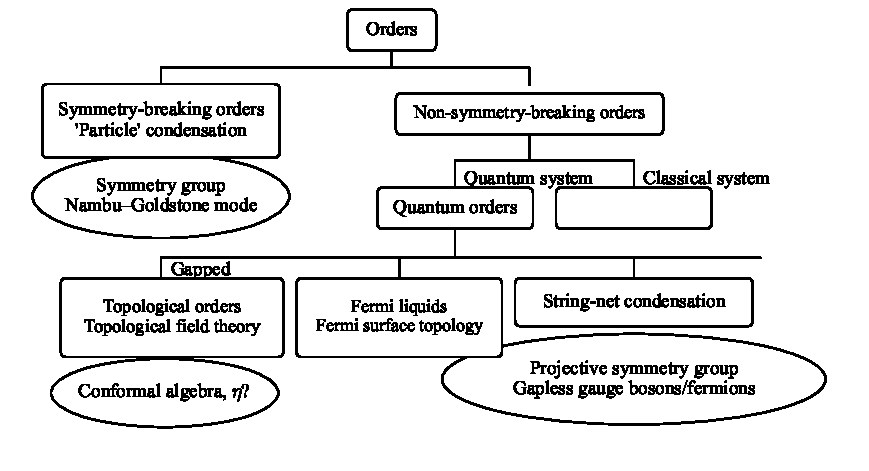
\includegraphics[width=0.72\textwidth]{fig_1.1.pdf}
\caption*{图 1.1\quad 物质中（以及真空中）不同序的分类。}
\end{figure}

已经证明，拓扑有序态的基态简并对\emph{任何}微扰都是稳健的（Wen and Niu, 1990）。因此，基态简并是一种可以用来刻画相的普适性质。拓扑简并基态的存在证明了拓扑序的存在。拓扑简并还可以用来执行容错量子计算（Kitaev, 2003）。

拓扑序的概念最近被推广为量子序（quantum order；Wen, 2002c），用以描述无能隙量子态中的新型序。理解量子序的一个方式，是看它如何纳入一个一般的序的分类方案（见图 1.1）。首先，不同的序可以分成两大类：对称性破缺序与非对称性破缺序。对称性破缺序可以用局域序参量描述，可以说其中包含点状物体的凝聚，凝聚的振幅对应于序参量。所有对称性破缺序都可以用朗道对称性破缺理论来理解。非对称性破缺序既不能用对称性破缺描述，也不能用与之相关的局域序参量和长程关联描述，因此是一种新型的序。如果一个量子系统（零温下的态）包含非对称性破缺序，那么就说该系统包含非平庸的量子序。我们看到，量子序无非是量子系统中的非对称性破缺序。

量子序还可以进一步分成许多子类。如果一个量子态有能隙，那么相应的量子序就称为拓扑序；拓扑有序态的低能有效理论将是拓扑场论（Witten, 1989）。第二类量子序出现在费米液体（或自由费米子系统）中，费米液体中不同的量子序由费米面拓扑来分类（Lifshitz, 1960）。第三类量子序来自弦网的凝聚（或简称弦网凝聚）（Wen, 2003a; Levin and Wen, 2003; Wen, 2003b），这一类量子序与“粒子”凝聚的对称性破缺序有某些相似之处。

我们知道，不同的对称性破缺序可以用对称群来分类：利用群论，我们可以把三维全部 230 种晶体序分类。对称性还在对称性破缺基态之上产生并保护无能隙集体激发——Nambu–Goldstone 玻色子。类似地，不同的弦网凝聚（及相应的量子序）可以用一个叫做投影对称群（projective symmetry group，PSG）的数学对象来分类（Wen, 2002c）。利用 PSG，我们可以把 100 多种具有相同对称性的不同二维自旋液体分类。正如对称群一样，PSG 也能产生并保护无能隙激发；然而，与对称群不同的是，PSG 产生并保护的是无能隙规范玻色子和费米子（Wen, 2002a,c; Wen and Zee, 2002）。正因为如此，我们可以说，光和无质量费米子可以有统一的起源：它们可以从弦网凝聚中演生出来。

按照图 1.1 中各序的分类，本书可以分为两部分。第一部分（第 3–5 章）讨论“粒子”凝聚产生的对称性破缺序。我们发展有效理论，研究来自序参量涨落的无能隙 Nambu–Goldstone 模的物理性质。这一部分讲述“声音的起源”以及其他 Nambu–Goldstone 模，还讲述超流体中旋子之间 $1/r^4$ 偶极相互作用定律的起源。第二部分（第 7–10 章）讨论量子序/拓扑序与弦网凝聚。同样，我们发展有效理论，研究低能集体模的物理性质。不过在这里，集体模来自凝聚弦网的涨落，并给出规范玻色子和费米子。因此，第二部分提供了“光与电子的一种起源”，以及其他规范玻色子和费米子的起源；它还提供了 $1/r^2$ 库仑定律（或更一般地，电磁学定律）的一种起源。

\section{光与费米子的起源}

\begin{keypoints}
\item 弦网凝聚为光与费米子的起源提供了一个答案。它统一了规范相互作用与费米统计。
\end{keypoints}

\begin{figure}[H]
\centering
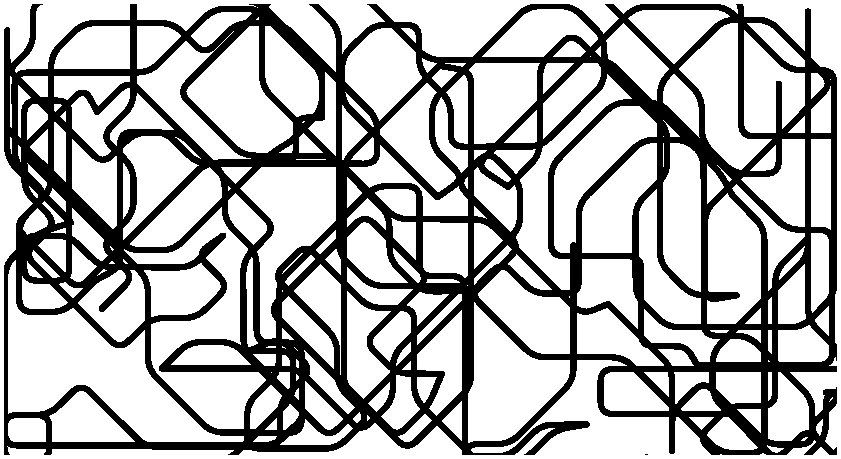
\includegraphics[width=0.72\textwidth]{fig_1.2.pdf}
\caption*{图 1.2\quad 我们的真空也许是一个充满弦网的态。弦网的涨落给出规范玻色子。弦的端点对应于电子、夸克等。}
\end{figure}

我们过去相信，要在理论中拥有光和费米子，就必须人为引进一个基本的 $U(1)$ 规范场和反对易的费米子场，因为在那个年代，我们还不知道有任何集体模的行为像规范玻色子和费米子。然而，由于过去二十年的进展，我们现在知道如何构造具有演生\emph{解禁闭}规范玻色子和/或费米子的\emph{局域玻色系统}（Foerster et al., 1980; Kalmeyer and Laughlin, 1987; Wen et al., 1989; Read and Sachdev, 1991; Wen, 1991a; Moessner and Sondhi, 2001; Motrunich and Senthil, 2002; Wen, 2002a; Kitaev, 2003; Levin and Wen, 2003）。特别地，人们可以在立方格子上构造丑陋的玻色自旋模型，其低能有效理论却是美丽的量子电动力学（QED）和量子色动力学（QCD），带有演生的光子、电子、夸克和胶子（Wen, 2003b）。

这引出了如下问题：自然界中的光和费米子，究竟是像 $U(1)\times SU(2)\times SU(3)$ 标准模型中那样，来自基本的 $U(1)$ 规范场和反对易场，还是来自我们真空中某种特定的量子序？库仑定律是自然界的基本定律，还是仅仅是一种演生现象？显然，假定光和费米子以及库仑定律都来自我们真空中的量子序，更为自然。从弦网凝聚、量子序与无质量规范/费米子激发之间的联系，我们看到弦网凝聚提供了一条统一光与费米子的途径。我们非常想就光和费米子的三个基本问题提出如下可能的回答。

\textbf{光和费米子是什么？}

光是（任意大小的）凝聚弦网的涨落；费米子是凝聚弦的端点。

\textbf{光和费米子从哪里来？}

光和费米子来自充满空间的弦网的集体运动（见图 1.2）。

\textbf{光和费米子为什么会存在？}

光和费米子之所以存在，是因为我们的真空碰巧具有一种叫做弦网凝聚的性质。

假如我们的真空当初选择的是“粒子”凝聚，那么低能下就将只有 Nambu–Goldstone 玻色子。那样的宇宙会非常乏味。弦网凝聚以及随之而来的光和费米子，则提供了一个有趣得多的宇宙——至少有趣到足以支撑智慧生命去研究光与费米子的起源。

\section{新奇比正确更重要}

\begin{keypoints}
\item 道可道，非常道；名可名，非常名。无名，天地之始；有名，万物之母。\footnote{这些是中国哲学家老子（Lao Zi）在 2500 多年前所写《道德经》的开头四句。原书英文是对它们的宽松直译。“道”兼有“道路”、“法则”、“品行”等含义。《道德经》存在许多差别很大的译本，上网搜索并比较这些不同的译本是一件趣事。下面是结合本书语境的一个译法：“可以表述的物理理论不可能是终极的理论。可以实施的分类不可能分类万物。不可表述的终极理论确实存在，并支配着宇宙的创生。已表述的理论描述我们每天看到的物质。”}
\item 能被言说的不会是新奇的；不能被言说的不会是正确的。
\end{keypoints}

在这篇引言中（以及本书的某些部分），我希望让读者感受到：在理论凝聚态物理中，我们从哪里来、现在站在哪里、正向何处去。我并不打算在这里总结公认的看法；相反，我想表达的是我个人的、有意夸张的、关于凝聚态物理和高能物理中许多基本问题的观点。这些观点和图像未必正确，但我希望它们具有启发性。从物理学历史的经验来看，我们可以放心地假定：现行的物理理论没有一个会是完全正确的。（按照老子（Lao Zi）的说法，能够写下来的理论不可能是永恒的理论，因为它受限于我们借以写下该理论的数学符号。）问题在于判定现行理论在哪个方面错了、该如何修正。这需要大量的想象力和激励。

\section{评注：基本粒子概念的演化}

\begin{keypoints}
\item 随着时间的流逝，基本粒子的地位不断被降级：从万物的砌块，降为（很可能）只是一个低微玻色模型的集体激发。
\end{keypoints}

地球曾被看作宇宙的中心。随着时间的流逝，它的地位降低为不过是宇宙中亿万颗行星之一。看来，基本粒子的概念可能也会有类似的命运。

在人类文明的开端，人们认识到物体可以被分割成越来越小的部分。中国哲学家提出，这种分割可以无限地继续下去，因而不存在基本粒子。希腊哲学家则假定分割不能无限地继续，于是存在终极而不可分割的粒子——万物的砌块。这可能是基本粒子的第一个概念。那些终极粒子被称为 \emph{atomos}。大量科学研究一直致力于寻找这些 \emph{atomos}。

大约在 1900 年，化学家发现所有物质都由几十种不同的粒子构成。人们操之过急地把它们命名为原子（atoms）。电子发现之后，人们认识到基本粒子比原子更小。现在，许多人相信光子、电子、夸克和其他几种粒子是基本粒子。这些粒子由一个叫做 $U(1)\times SU(2)\times SU(3)$ 标准模型的场论描述。

尽管 $U(1)\times SU(2)\times SU(3)$ 标准模型是一个非常成功的理论，现在大多数高能物理学家相信，它并不是终极的万物理论。$U(1)\times SU(2)\times SU(3)$ 标准模型可能是从一个更深层结构中演生出来的有效理论。问题是：标准模型可能从什么样的结构中演生出来？

一个提案是大统一理论，其中 $U(1)\times SU(2)\times SU(3)$ 规范群被提升为 $SU(5)$ 甚至更大的规范群（Georgi and Glashow, 1974）。大统一理论把 $U(1)\times SU(2)\times SU(3)$ 标准模型中的粒子归入非常漂亮而且简单得多的结构。然而，我想指出，我并不认为在大统一理论中光子、电子和其他基本粒子是演生的。在大统一理论中，规范结构和费米统计是基本的，其含义是：想要有规范玻色子和费米子，唯一的办法就是引进矢量规范场和反对易费米子场。因此，为了拥有光子、电子和其他基本粒子，我们必须人为引进相应的规范场和费米子场。所以，规范玻色子和费米子是被人为加进大统一理论的；它们并不是从更简单的结构中演生出来的。

第二个提案是超弦理论（Green et al., 1988; Polchinski, 1998）。某些超弦模型可以给出有效的 $U(1)\times SU(2)\times SU(3)$ 标准模型，外加许多额外的（近）无质量激发。规范玻色子和引力子是演生的，因为超弦理论本身不包含规范场。然而，费米统计不是演生的：电子和夸克来自 $(1+1)$ 维世界面上的反对易费米子场。我们看到，在超弦理论中，规范玻色子和规范结构不是基本的，但费米统计和费米子仍然是基本的。

最近，人们意识到可能存在第三种可能——弦网凝聚。Banks et al.（1977）和 Foerster et al.（1980）首先指出，光可以作为局域玻色模型的低能集体模演生出来。Levin and Wen（2003）指出，即使是三维费米子，也可以作为凝聚弦的端点从局域玻色模型中演生出来。把这两个结果结合起来，我们发现：只要玻色模型具有弦网凝聚，光子、电子、夸克和胶子（或者更精确地说，$U(1)\times SU(2)\times SU(3)$ 标准模型的 QED 和 QCD 部分）就可以从局域玻色模型中演生出来（Wen, 2002a, 2003b）。这一提案的诱人之处在于，规范玻色子和费米子有着统一的起源。在弦网凝聚的图像中，规范结构和费米统计都不是基本的；所有基本粒子都是演生的。

然而，第三个提案也有一个问题：由于手征费米子问题，我们还不知道如何产生标准模型的 $SU(2)$ 部分。自然界有五个深奥之谜，即全同粒子、费米统计、规范结构、手征费米子和引力。弦网凝聚只回答了前三个谜；还剩两个有待解决。

% ==================================================================
% 新增术语（本章新增，供术语表追加）：
%   phonon 声子；roton 旋子；sound wave 声波；dipolar interaction 偶极相互作用；
%   building block 砌块；black box 黑箱；fractional statistics 分数统计；
%   non-abelian statistics 非阿贝尔统计；Nambu–Goldstone mode/boson Nambu–Goldstone 模/玻色子；
%   spontaneous breaking of continuous symmetry 连续对称性自发破缺；
%   translational symmetry breaking 平移对称性破缺；topological field theory 拓扑场论；
%   fault-tolerant quantum computation 容错量子计算；edge states 边缘态；
%   ground-state degeneracy 基态简并；natural selection 自然选择；
%   grand unified theories 大统一理论；superstring theory 超弦理论；graviton 引力子；
%   gluon 胶子；world sheet 世界面；chiral fermion problem 手征费米子问题；
%   identical particles 全同粒子；random systems 无序系统；many-boson system 多玻色子系统；
%   standard model 标准模型；atomos atomos（希腊语“不可分”，原子一词的来源）
% ==================================================================

 % 本文件由 scripts/assemble.py 自动装配，勿手改（改 parts/ 后重跑）
% 第2章 量子力学的路径积分表述

%--A-TAIL--
\begin{align*}
\operatorname{Det}(M_N) &= 2\cosh(u)\operatorname{Det}(M_{N-1}) - \operatorname{Det}(M_{N-2}),\\
\operatorname{Det}(M_1) &= 2\cosh(u), \qquad \operatorname{Det}(M_2) = 4\cosh^2(u) - 1.
\end{align*}
% 第2章 PATH INTEGRAL FORMULATION OF QUANTUM MECHANICS
\chapter{量子力学的路径积分表述}

本书讨论多体系统的量子行为。然而，以波函数和薛定谔方程为核心的标准量子理论表述并不适用于多体系统。在本章中，我们为量子理论引入半经典图像（semiclassical picture）与路径积分（path integral）表述。路径积分表述可以很方便地应用于多体系统。这里，我们将以单粒子系统为具体例子来建立这套表述。我们还将应用路径积分表述来研究量子摩擦、简单量子线路等问题。

\section{半经典图像与路径积分}

\begin{keypoints}
\item 半经典图像与路径积分表述使我们能够直观地构想量子行为；它们给了我们一个量子系统的全局图像。
\end{keypoints}

当我们在思考一个物理问题或试图理解一个现象时，在头脑中有一幅图像、从而能在心里构想出谜题各个碎片之间的联系，是非常重要的。对于经典系统，这种心理构想要容易些，因为经典系统的图像与我们日常生活实际所见相当接近。然而，当我们考虑量子系统时，构想就困难得多了。这是因为量子世界与我们每天所见并不相似。在经典世界中，我们看到各种物体。稍加抽象，我们便把这些物体视为粒子的集合。粒子的概念是经典物理学中最重要的概念。它如此简单而平淡，以至于人们视之为理所当然，懒得去为这样一个显而易见的真理专门表述成一条物理定律。然而，正是这个显而易见的真理在量子世界中被证明是错误的。具有位置和速度的粒子概念在量子世界中根本不存在。于是，挑战就在于：在一个连粒子（即构成物体的积木块）概念都不存在的量子世界里，如何去构想任何东西。

路径积分表述正是用经典世界的图像来描述量子世界的一种尝试。换言之，它是架在经典世界（我们拥有经验与图像之处）与量子世界（代表实在之处）之间的一座桥梁。路径积分表述将帮助我们借助相应经典系统的图像来直观地把握量子行为。

\subsection{粒子的传播子}

\begin{keypoints}
\item 传播子的概念。
\item 传播子在 $\omega$ 空间中的极点结构。
\end{keypoints}

考虑一个一维粒子：
\begin{equation*}
H = \frac{1}{2m}p^2 + V(x) \tag{2.1.1}
\end{equation*}
时间演化算符（time evolution operator）
\begin{equation*}
U(t_b,t_a) = \mathrm{e}^{-\mathrm{i}\hbar^{-1}(t_b-t_a)H} = \mathrm{e}^{-\mathrm{i}(t_b-t_a)H}
\end{equation*}
完全决定了系统的行为与性质。本节中我们总假定 $t_b > t_a$。全书我们取 $\hbar = 1$。

$U$ 在坐标基下的矩阵元为
\begin{equation*}
\mathrm{i}G(x_b,t_b,x_a,t_a) \equiv \langle x_b|U(t_b,t_a)|x_a\rangle
\end{equation*}
它表示：若粒子在时刻 $t_a$ 位于 $x_a$，则在时刻 $t_b$ 于位置 $x_b$ 找到该粒子的概率振幅。这里 $G(x_b,t_b,x_a,t_a)$ 称为传播子（propagator），它对我们的单粒子量子系统给出了完整而完备的描述。

显然，传播子 $G$ 满足薛定谔方程
\begin{equation*}
\mathrm{i}\partial_t G(x,t,x_a,t_a) = H G(x,t,x_a,t_a)
\end{equation*}
初条件为
\begin{equation*}
G(x,t_a,x_a,t_a) = (-\mathrm{i})\,\delta(x-x_a)
\end{equation*}
求解薛定谔方程，得到 $V(x)=0$ 时自由粒子的传播子
\begin{equation*}
G(x_b,x_a,t) = (-\mathrm{i})\left(\frac{m}{2\pi\mathrm{i}t}\right)^{1/2} \exp\left[\frac{\mathrm{i}m(x_b-x_a)^2}{2t}\right] \tag{2.1.2}
\end{equation*}
其中 $t = t_b - t_a$。

我们也可以用能量本征态 $|n\rangle$（能量为 $\epsilon_n$）来展开 $U$。在新基下，传播子具有以下更简单的形式：
\begin{equation*}
G_E(n_b,t_b,n_a,t_a) \equiv (-\mathrm{i})\langle n_b|U(t_b,t_a)|n_a\rangle = (-\mathrm{i})\mathrm{e}^{-\mathrm{i}\epsilon_n(t_b-t_a)}\delta_{n_b,n_a}
\end{equation*}
在频率空间中，它由下式给出：
\begin{align*}
G_E(n_b,n_a,\omega) &\equiv \int_0^{\infty} \mathrm{d}t\, G_E(n_b,t_a+t,n_a,t_a)\,\mathrm{e}^{\mathrm{i}t\omega-0^+t}\\
&= \frac{1}{\omega-\epsilon_{n_a}+\mathrm{i}0^+}\,\delta_{n_b,n_a}
\end{align*}
它在每个能量本征值处都有一个单极点。这里 $0^+$ 是一个无穷小的正数，引入它是为了使积分收敛。坐标空间中的传播子具有类似的结构：
\begin{align*}
G(x_b,x_a,t) &= \sum_n \langle x_b|n\rangle\langle n|x_a\rangle G_E(n,n,t) = \sum_n \langle x_b|n\rangle\langle n|x_a\rangle(-\mathrm{i})\mathrm{e}^{-\mathrm{i}\epsilon_n t}\\
G(x_b,x_a,\omega) &= \sum_n \frac{\langle x_b|n\rangle\langle n|x_a\rangle}{\omega-\epsilon_n+\mathrm{i}0^+}
\end{align*}
我们看到，通过分析 $G(x_b,x_a,\omega)$ 的极点结构，可以获得关于能量本征值的信息。

为了重新得到时间中的传播子
\begin{equation*}
G_E(n_b,n_a,t) = \int \frac{\mathrm{d}\omega}{2\pi}\, \frac{1}{\omega-\epsilon_{n_a}+\mathrm{i}0^+}\,\delta_{n_b,n_a}\,\mathrm{e}^{-\mathrm{i}t\omega}
\end{equation*}
当 $t>0$ 时，我们需要在复 $\omega$ 平面的下半平面选取围道，$t<0$ 时则需在上半平面选取围道，以使沿围道的积分有限。由于 $0^+$ 使极点出现在复 $\omega$ 平面实轴的略下方，我们得到
\begin{equation*}
G_E(n_b,n_a,t) = (-\mathrm{i})\,\mathrm{e}^{-\mathrm{i}\epsilon_n(t_b-t_a)}\delta_{n_b,n_a}\,\Theta(t)
\end{equation*}
其中
\begin{equation*}
\Theta(t) = \left\{\begin{array}{ll} 1, & t>0\\ 0, & t<0 \end{array}\right. \tag{2.1.3}
\end{equation*}

\subsection*{问题 2.1.1}

证明：在频率空间中，有
\begin{equation*}
G(x_b,x_a,\omega) = \sum_n \frac{\psi_n(x_b)\psi_n^{\dagger}(x_a)}{\omega-\epsilon_n}
\end{equation*}
其中 $\psi_n$ 为能量本征函数。谐振子的传播子具有如下形式：
\begin{equation*}
G(x_b,t,x_a,0) = (-\mathrm{i})\left(\frac{m\omega_0}{2\pi\mathrm{i}\sin(t\omega_0)}\right)^{1/2} \exp\left(\frac{\mathrm{i}m\omega_0}{2\pi\sin(t\omega_0)}\big[(x_b^2+x_a^2)\cos(\omega_0 t) - 2x_bx_a\big]\right)
\end{equation*}
（译注：按标准结果并参照问题 2.1.6，指数上的分母应为 $2\sin(t\omega_0)$，原书排印为 $2\pi\sin(t\omega_0)$。）研究并解释谐振子的 $G(0,0,\omega)$ 的极点结构。（提示：尝试把 $G(0,t,0,0)$ 展开成 $\sum C_n\mathrm{e}^{-\mathrm{i}t\epsilon_n}$ 的形式。）

\subsection*{问题 2.1.2}

试求三维自由粒子在波矢与频率空间中的传播子 $G_E(k_b,k_a,\omega)$。

\subsection{传播子的路径积分表示}

\begin{keypoints}
\item 路径积分是量子物理中叠加原理的一种特殊表示。
\end{keypoints}

量子系统的路径积分表述，其精神实质非常简单。考虑一个粒子经由中间态 $|n\rangle$（$n = 1, 2, \dots$）从位置 $|x_a\rangle$ 传播到位置 $|x_b\rangle$。设经由态 $|n\rangle$ 从 $|x_a\rangle$ 到 $|x_b\rangle$ 的振幅为 $A_n$，则从 $|x_a\rangle$ 到 $|x_b\rangle$ 的总振幅为 $\sum_n A_n$。现在设想我们把从 $|x_a\rangle$ 到 $|x_b\rangle$ 的传播分成许多时间切片，每个时间切片拥有自己的一组中间态。从 $|x_a\rangle$ 到 $|x_b\rangle$ 的传播可以看成穿过各时间切片上中间态的所有路径之和。这就给出了传播振幅的路径积分表示的一幅图像。

为了给上述图像找到一个数学表示，我们注意到从 $|x_a\rangle$ 到 $|x_b\rangle$ 的振幅由时间演化算符 $U$ 在位置空间中的矩阵元描述。$U$ 满足
\begin{equation*}
U(t_b,t_a) = U(t_b,t)\,U(t,t_a)
\end{equation*}
于是，传播子满足
\begin{equation*}
\mathrm{i}G(x_b,t_b,x_a,t_a) = \int \mathrm{d}x\; \mathrm{i}G(x_b,t_b,x,t)\,\mathrm{i}G(x,t,x_a,t_a) \tag{2.1.4}
\end{equation*}

\begin{figure}[H]
\centering
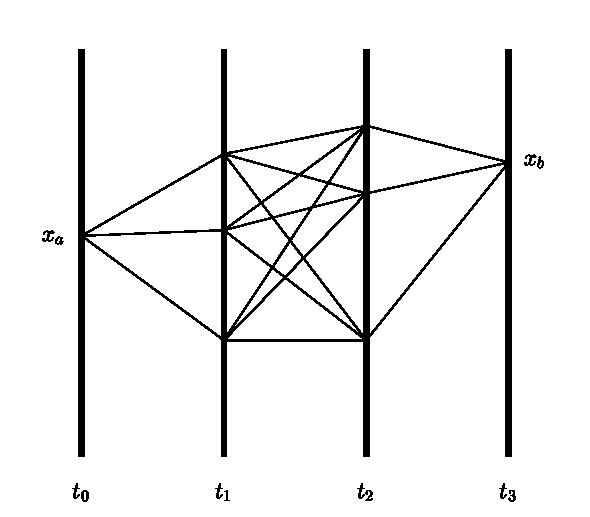
\includegraphics[width=0.72\textwidth]{fig_2.1.pdf}
\caption*{图 2.1\quad 总振幅是连接 $x_a$ 与 $x_b$ 的所有路径所对应的振幅之和。}
\end{figure}

让我们把时间区间 $[t_a,t_b]$ 分成 $N$ 个等长的小段，每段长度 $\Delta t = \frac{t_b-t_a}{N}$。将式 (2.1.4) 使用 $N-1$ 次，我们得到
\begin{align*}
\mathrm{i}G(x_b,t_b,x_a,t_a) &= \int \mathrm{d}x_1...\mathrm{d}x_{N-1} \prod_{j=1}^{N} \mathrm{i}G(x_j,t_j,x_{j-1},t_{j-1})\\
&= A^N \int \prod_i \mathrm{d}x_i\, \exp\left(\mathrm{i} \sum \Delta t\, L\Big(t_j, \frac{x_j+x_{j-1}}{2}, \frac{x_j-x_{j-1}}{\Delta t}\Big)\right)\\
&\equiv \int \mathcal{D}[x(t)]\; \mathrm{e}^{\mathrm{i}\int \mathrm{d}t\, L(t,x,\dot{x})} \tag{2.1.5}
\end{align*}
其中 $(t_0,x_0)=(t_a,x_a)$，$(t_N,x_N)=(t_b,x_b)$，且
\begin{equation*}
\mathrm{i}\Delta t\, L\Big(t_i, \frac{x_i+x_{i-1}}{2}, \frac{x_i-x_{i-1}}{\Delta t}\Big) = \ln[\mathrm{i}G(x_i,t_i,x_{i-1},t_{i-1})/A] \tag{2.1.6}
\end{equation*}

假定适当选取 $A$ 之后，式 (2.1.6) 中 $L$ 的定义在 $\Delta t \to 0$ 极限下有意义，那么式 (2.1.5) 就是传播子的路径积分表示。

在路径积分表示中，每条路径都被赋予一个振幅 $\mathrm{e}^{\mathrm{i}\int \mathrm{d}t\,L}$。传播子不过是连接 $x_a$ 与 $x_b$ 的所有路径所对应的振幅之和（图 2.1）。这样的求和是一个无穷维积分，而式 (2.1.5) 给出了计算这种无穷维积分的一种方式。

现在让我们对我们的单粒子系统 (2.1.1) 计算 $L(t,x,\dot{x})$。对于自由粒子系统，我们可以利用式 (2.1.2) 来计算 $L(t,x,\dot{x})$。下面我们将对由 $H = \frac{p^2}{2m} + V(x)$ 描述的更一般的单粒子系统计算 $L$。注意到，对于小的 $\Delta t$，有
\begin{equation*}
\exp\left(-\mathrm{i}\Big[\frac{p^2}{2m} + V(x)\Big]\Delta t\right) = \exp\left(-\mathrm{i}\frac{p^2}{2m}\Delta t\right)\exp\left(-\mathrm{i}V(x)\Delta t\right) + O(\Delta t^2)
\end{equation*}
因此
\begin{align*}
&\mathrm{i}G(x_{i-1},t_{i-1},x_i,t_i)\\
&\qquad = \langle x_i| \exp\left(-\mathrm{i}\frac{p^2}{2m}\Delta t\right)\exp\left(-\mathrm{i}V(x)\Delta t\right) |x_{i-1}\rangle + O(\Delta t^2)\\
&\qquad = \langle x_i| \exp\left(-\mathrm{i}\frac{p^2}{2m}\Delta t\right) |x_{i-1}\rangle\, \exp\left(-\mathrm{i}V(x_{i-1})\Delta t\right) + O(\Delta t^2)
\end{align*}
插入 $\int |p\rangle \frac{\mathrm{d}p}{2\pi}\langle p| = 1$ 并利用 $\langle p|x\rangle = \exp(-\mathrm{i}px)$，我们得到
\begin{align*}
&\mathrm{i}G(x_{i-1},t_{i-1},x_i,t_i)\\
&\qquad = \int \frac{\mathrm{d}p_i}{2\pi}\, \exp\left(\mathrm{i}\big[p_i\frac{x_i-x_{i-1}}{\Delta t} - \frac{p_i^2}{2m} - V(x_i)\big]\Delta t\right) + O(\Delta t^2) \tag{2.1.7}\\
&\qquad = \left(\frac{m}{2\pi\mathrm{i}\Delta t}\right)^{1/2} \exp\left(\mathrm{i}\big[\frac{m}{2}\frac{(x_i-x_{i-1})^2}{\Delta t^2} - V\big(\frac{x_i+x_{i-1}}{2}\big)\big]\Delta t\right) \tag{2.1.8}
\end{align*}
由式 (2.1.6) 可见
\begin{align*}
&L(x,\dot{x}) = \frac{m}{2}\dot{x}^2 - V(x) \tag{2.1.9}\\
&A \equiv \left(\frac{m}{2\pi\mathrm{i}\Delta t}\right)^{1/2}
\end{align*}
于是，传播子的路径积分表示为
\begin{align*}
\mathrm{i}G(x_b,t_b,x_a,t_a) &= \int \mathrm{d}x_1...\mathrm{d}x_{N-1} \prod_{j=1}^{N} \mathrm{i}G(x_j,t_j,x_{j-1},t_{j-1})\\
&= \left(\frac{m}{2\pi\mathrm{i}\Delta t}\right)^{N/2} \int \mathrm{d}x_1...\mathrm{d}x_{N-1}\; \mathrm{e}^{\mathrm{i}\int \mathrm{d}t\,[\frac{m}{2}\dot{x}^2 - V(x)]} \tag{2.1.10}
\end{align*}

上面算出的 $L(x,\dot{x})$ 正是相应经典系统的拉格朗日量。因此，原则上一旦我们了解了一个经典系统（通过拉格朗日量来描述），就可以利用同一个拉格朗日量，通过路径积分得到相应的量子系统。

我们也可以把式 (2.1.7) 代入式 (2.1.5)，得到
\begin{align*}
&\mathrm{i}G(x_b,t_b,x_a,t_a)\\
&\qquad = \left(\frac{1}{2\pi}\right)^{N} \int \mathrm{d}x_1...\mathrm{d}x_{N-1}\,\mathrm{d}p_1...\mathrm{d}p_N\; \exp\left(\mathrm{i}\sum_{i=1}^{N}\big[p_i\frac{x_i-x_{i-1}}{\Delta t} - \frac{p_i^2}{2m} - V(x_i)\big]\right)\\
&\qquad \equiv \int \mathcal{D}[x(t)]\,\mathcal{D}[p(t)]\; \mathrm{e}^{\mathrm{i}\int \mathrm{d}t\,[p\dot{x} - H(x,p)]} \tag{2.1.11}
\end{align*}
这是相空间（phase space）中的路径积分。这里 $H(x,p)$ 是经典哈密顿量。如果我们把相空间测度定义为
\begin{equation*}
\mathcal{D}[x(t)]\,\mathcal{D}[p(t)] \equiv \prod_1^{N-1} \mathrm{d}x_i \prod_1^{N} \frac{\mathrm{d}p_i}{2\pi} \tag{2.1.12}
\end{equation*}
那么哈密顿量 $H$ 就与经典的完全相同。看起来，相空间路径积分比坐标空间路径积分更为基本，因为那个讨厌的系数 $A$（见式 (2.1.9)）不再出现在路径积分的测度之中。我们还注意到，上述相空间测度含有 $N-1$ 个 $\mathrm{d}x$ 积分和 $N$ 个 $\mathrm{d}p$ 积分。

我们知道，给拉格朗日量加上一个全时间导数项，即 $L \to L + \frac{\mathrm{d}f(x)}{\mathrm{d}t}$，并不影响经典动力学。然而，这样的改变确实会影响量子传播子，只是以一种平凡的方式：
\begin{equation*}
G(x_b,t_b,x_a,t_a) \to G(x_b,t_b,x_a,t_a)\,\mathrm{e}^{\mathrm{i}[f(x_b)-f(x_a)]}
\end{equation*}

\subsection*{问题 2.1.3}

相干态路径积分：

考虑谐振子 $H = \omega\hat{a}^{\dagger}\hat{a}$。由复数 $a$ 标记的相干态（coherent state）$|a\rangle$ 是 $\hat{a}$ 的本征态：$\hat{a}|a\rangle = a|a\rangle$。我们可以定义相干态传播子
\begin{equation*}
\mathrm{i}G(a_b,t_b,a_a,t_a) = \langle a_b|U(t_b,t_a)|a_a\rangle
\end{equation*}
利用相干态的完备性
\begin{equation*}
\int \frac{\mathrm{d}^2a}{\pi} |a\rangle\langle a| = 1
\end{equation*}
（其中 $\mathrm{d}^2a = \mathrm{d}\mathrm{Re}(a)\,\mathrm{d}\mathrm{Im}(a)$）以及内积
\begin{equation*}
\langle a|a'\rangle = \mathrm{e}^{-|a|^2/2}\,\mathrm{e}^{-|a'|^2/2}\,\mathrm{e}^{a^*a'}
\end{equation*}
证明 $G$ 的路径积分表示为
\begin{equation*}
\mathrm{i}G(a_b,t_b,a_a,t_a) = \int \pi^{-N+1}\mathcal{D}^2[a(t)]\; \mathrm{e}^{\mathrm{i}\int_{t_a}^{t_b}\mathrm{d}t\,[\mathrm{i}\frac{1}{2}(a^{\dagger}\dot{a} - a\dot{a}^{\dagger}) - \omega a^{\dagger}a]}
\end{equation*}
其中 $\mathcal{D}^2[a(t)] = \prod_{j=1}^{N-1}\mathrm{d}^2a_j$。证明相干态路径积分中的拉格朗日量
\begin{equation*}
L = \mathrm{i}\frac{1}{2}(a^{\dagger}\dot{a} - a\dot{a}^{\dagger}) - \omega a^{\dagger}a
\end{equation*}
与相空间路径积分中的拉格朗日量
\begin{equation*}
L = p\dot{x} - H
\end{equation*}
仅相差一个全时间导数项。

\subsection{配分函数的路径积分表示}

\begin{keypoints}
\item 路径积分也可以用来研究统计系统。
\end{keypoints}

当我们考虑量子系统在有限温度下的统计性质时，配分函数（partition function）非常有用。我们的单粒子系统 (2.1.1) 的配分函数为
\begin{equation*}
Z(\beta) = \operatorname{Tr}\left(\mathrm{e}^{-\beta H}\right) = \int \mathrm{d}x\; \mathcal{G}(x,x,\beta)
\end{equation*}
其中 $\beta = \frac{1}{T}$ 是温度的倒数，而
\begin{equation*}
\mathcal{G}(x_b,x_a,\beta) \equiv \langle x_b|\mathrm{e}^{-\beta H}|x_a\rangle
\end{equation*}
可以看作虚时（imaginary time）中的传播子。上一节的计算可以重复进行，我们得到 $\mathcal{G}$ 的如下路径积分表示：
\begin{equation*}
\mathcal{G}(x_b,x_a,\tau) = A_{\tau}^N \int \mathcal{D}[x(\tau)]\; \mathrm{e}^{-\int_0^{\tau} \big[\frac{m}{2}\big(\frac{\mathrm{d}x}{\mathrm{d}\tau}\big)^2 + V(x)\big]\mathrm{d}\tau'} \tag{2.1.13}
\end{equation*}
\begin{equation*}
A_{\tau} \equiv \left(\frac{m}{2\pi\Delta\tau}\right)^{1/2} \tag{2.1.14}
\end{equation*}
相应的相空间路径积分为
\begin{equation*}
\mathcal{G}(x_b,x_a,\tau) = \int \mathcal{D}[x(\tau)]\,\mathcal{D}[p(\tau)]\; \mathrm{e}^{-\int_0^{\tau} \big[\frac{p^2}{2m} + V(x) - \mathrm{i}p\frac{\mathrm{d}x}{\mathrm{d}\tau}\big]\mathrm{d}\tau'} \tag{2.1.15}
\end{equation*}
于是，配分函数可以写成
\begin{align*}
Z(\beta) &= \int \mathcal{D}[x(\tau)]\,\mathcal{D}[p(\tau)]\; \mathrm{e}^{-\oint \big[\frac{p^2}{2m} + V(x) - \mathrm{i}p\frac{\mathrm{d}x}{\mathrm{d}\tau}\big]\mathrm{d}\tau'}\\
&= A_{\tau}^N \int \mathcal{D}[x(\tau)]\; \mathrm{e}^{-\oint \big[\frac{m}{2}\big(\frac{\mathrm{d}x}{\mathrm{d}\tau}\big)^2 + V(x)\big]\mathrm{d}\tau'}
\end{align*}
其中 $x(0) = x(\beta)$，$p(0) = p(\beta)$，测度略有不同：$\mathcal{D}[x(\tau)] = \prod_1^{N}\mathrm{d}x_j$，$\mathcal{D}[x(\tau)]\mathcal{D}[p(\tau)] = \prod_1^{N}\frac{\mathrm{d}x_j\mathrm{d}p_j}{2\pi}$。如果我们把虚时方向紧致化，那么配分函数就不过是缠绕在虚时方向上的各条加权回路的和。

路径积分 (2.1.13) 与 (2.1.15) 常被称为虚时路径积分，因为通过解析延拓（analytic continuation）
\begin{equation*}
\tau \to \mathrm{e}^{\mathrm{i}\theta}t \to \mathrm{i}t
\end{equation*}
即让 $\theta$ 从 $0$ 连续变到 $\frac{\pi}{2}$，它们可以被映射为实时路径积分 (2.1.5) 与 (2.1.11)。在虚时路径积分中把 $\tau$ 换成 $\mathrm{e}^{\mathrm{i}\theta}t$ 之后，我们得到
\begin{equation*}
\mathcal{G}\big(x_b,x_a,t\mathrm{e}^{\mathrm{i}\theta}\big) = \left(\frac{m}{2\pi\mathrm{e}^{\mathrm{i}\theta}\Delta t}\right)^{N/2} \int \mathcal{D}[x(t)]\; \mathrm{e}^{-\int_0^{t} \big[\frac{m}{2}\big(\frac{\mathrm{d}x}{\mathrm{d}t}\big)^2\mathrm{e}^{-\mathrm{i}\theta} + V(x)\mathrm{e}^{\mathrm{i}\theta}\big]\mathrm{d}t'}
\end{equation*}
可以发现，只要 $-\frac{\pi}{2} < \theta < \frac{\pi}{2}$，这些积分总是收敛的。

作为解析延拓的结果，实时传播子与虚时传播子之间的关系为
\begin{equation*}
\boxed{\;\mathcal{G}(x_b,x_a,\tau)\big|_{\tau=\mathrm{i}t} = \mathrm{i}G(x_b,x_a,t)\;}
\end{equation*}
借助解析延拓，我们常常可以通过计算相应的虚时传播子来得到实时传播子，而虚时传播子的计算往往更为简单。

\subsection*{问题 2.1.4}

推导式 (2.1.13) 与式 (2.1.15) 所给出的虚时传播子的路径积分表示。

\subsection{路径积分的计算}

\begin{keypoints}
\item 当量子涨落不强时，驻定路径（stationary path）以及驻定路径附近的二次涨落支配着路径积分。
\item 驻定路径是经典运动方程的解。
\end{keypoints}

上面我们推导了量子传播子的一种路径积分表示。这里我们将直接计算路径积分，并证实路径积分确实重新给出量子传播子。这一计算也使我们得以对路径积分和量子传播子获得一些直观的理解。

让我们考虑半经典极限，即典型路径的作用量（action）远大于 $\hbar = 1$ 的极限。在这个极限下，当我们对一段范围内的路径积分时，相位 $\mathrm{e}^{\mathrm{i}S}$ 变化剧烈，不同路径的贡献相互抵消。然而，在满足
\begin{equation*}
S[x_c(t) + \delta x(t)] = S[x_c(t)] + O[(\delta x)^2] \tag{2.1.16}
\end{equation*}
的驻定路径 $x_c(t)$ 附近，所有路径都具有相同的相位，发生相长干涉。因此，在半经典极限下，驻定路径及其邻近的路径对路径积分的贡献占主导地位。我们还注意到，驻定路径不过是作用量 $S[x(t)]$ 的经典运动路径。这样，路径积分表示使我们能清楚地看到经典运动与量子传播子之间的关系：粒子的量子传播基本上沿着由经典运动方程确定的路径行进，只是带有某种“晃动”。这种晃动称为量子涨落（quantum fluctuation）。路径积分表示使我们能够估计量子涨落的大小。更确切地说，围绕驻定路径 $x_c(t)$ 的、满足
\begin{equation*}
\big|S[x_c(t)+\delta x(t)] - S[x_c(t)]\big| \sim \pi/2
\end{equation*}
的涨落 $\delta x(t)$ 会对传播子有很大贡献，因而代表一个典型的量子涨落。

让我们先对自由粒子计算路径积分 (2.1.5)。此时，式 (2.1.5) 成为
\begin{align*}
&\mathrm{i}G(x_b,t_b,x_a,t_a)\\
&\qquad = \left(\frac{m}{2\pi\mathrm{i}\Delta t}\right)^{N/2} \int \mathrm{d}x_1...\mathrm{d}x_{N-1} \prod_{i=1}^{N} \exp\left(\mathrm{i}\big[\frac{m}{2}\frac{(x_i-x_{i-1})^2}{\Delta t^2}\big]\Delta t\right) \tag{2.1.17}
\end{align*}
自由粒子的经典路径（即驻定路径）为
\begin{equation*}
x_c(t) = x_a + \frac{x_b-x_a}{t_b-t_a}(t-t_a)
\end{equation*}
其经典作用量为
\begin{equation*}
S_c(x_b,t_b,x_a,t_a) = \frac{m(x_b-x_a)^2}{2(t_b-t_a)}
\end{equation*}
引入围绕经典路径的涨落
\begin{equation*}
\delta x_j = x_j - x_c(t_j), \qquad t_j = t_a + j\Delta t
\end{equation*}
路径积分 (2.1.17) 可以改写为
\begin{align*}
&\mathrm{i}G(x_b,t_b,x_a,t_a)\\
&\qquad = \left(\frac{m}{2\pi\mathrm{i}\Delta t}\right)^{N/2} \mathrm{e}^{\mathrm{i}S_c} \int \mathrm{d}x_1...\mathrm{d}x_{N-1} \exp\left(\mathrm{i}\sum_{j,k=1,N-1} \delta x_j M_{jk}\delta x_k\right)\\
&\qquad = \left(\frac{m}{2\pi\mathrm{i}\Delta t}\right)^{N/2} \sqrt{\frac{\pi^{N-1}}{\operatorname{Det}(-\mathrm{i}M)}}\; \mathrm{e}^{\mathrm{i}S_c}
\end{align*}
其中这个 $(N-1)\times(N-1)$ 矩阵为
\begin{equation*}
M = \frac{m}{2\Delta t}\left(\begin{array}{cccc} 2 & -1 & 0 & \dots\\ -1 & 2 & -1 & \dots\\ 0 & -1 & 2 & \dots\\ \dots & \dots & \dots & \dots \end{array}\right)
\end{equation*}
在上面的例子中，我们用到了以下关于高斯积分（Gaussian integral）的重要公式：
\begin{equation*}
\int \mathrm{d}x_1...\mathrm{d}x_{N-1}\; \exp\left(\mathrm{i}\sum_{j,k=1,N-1} x_j M_{jk}x_k\right) = \frac{\sqrt{\pi}^{\,N-1}}{\sqrt{\operatorname{Det}(-\mathrm{i}M)}}
\end{equation*}
我们看到，传播子由经典作用量 $\mathrm{e}^{\mathrm{i}S_c}$ 乘以一个由高斯积分（或相应的行列式）给出的系数构成。该系数由围绕经典路径的量子涨落 $\delta x$ 决定。

我们注意到，只有 $\mathrm{e}^{\mathrm{i}S_c}$ 项依赖 $x_a$ 与 $x_b$，其余各项仅依赖 $t_b - t_a \equiv t$。于是我们有
\begin{equation*}
G(x_b,t_b,x_a,t_a) = A(t_b-t_a)\,\mathrm{e}^{\mathrm{i}S_c(x_b,t_b,x_a,t_a)} \tag{2.1.18}
\end{equation*}
由归一化条件
\begin{equation*}
\int \mathrm{d}x_b\; G(x_b,t_b,x_a,t_a)G^*(x_b,t_b,x_a',t_a) = \delta(x_a-x_a')
\end{equation*}
我们得到
\begin{equation*}
A(t) = \left(\frac{m}{2\pi\mathrm{i}t}\right)^{1/2}\mathrm{e}^{\mathrm{i}\phi}
\end{equation*}
只要取相位 $\phi = 0$，它就与标准结果一致。

要直接计算 $A(t)$，我们需要计算 $\operatorname{Det}(M)$。下面我们将讨论一些可用于计算行列式的技巧。我们先考虑以下 $N\times N$ 矩阵：
\begin{equation*}
M_N = \left(\begin{array}{cccc} 2\cosh(u) & -1 & 0 & \dots\\ -1 & 2\cosh(u) & -1 & \dots\\ 0 & -1 & 2\cosh(u) & \dots\\ \dots & \dots & \dots & \dots \end{array}\right)
\end{equation*}
可以证明

% ------------------------------------------------------------
% 新增术语（ch2_a，待并入术语表"新增术语"区）：
%   stationary path 驻定路径
%   analytic continuation 解析延拓
%   phase space 相空间
%   Gaussian integral 高斯积分
%   time evolution operator 时间演化算符
%   contour 围道
%   constructive interference 相长干涉
%   action 作用量
%   law of superposition 叠加原理
%   energy eigenstate 能量本征态
%   energy eigenfunction 能量本征函数
%   time slice 时间切片
%   quantum friction 量子摩擦
%   quantum circuit 量子线路
%   matrix element 矩阵元
% ------------------------------------------------------------

上面的差分方程可以用拟设 $\operatorname{Det}(M_N)=a\mathrm{e}^{nu}+b\mathrm{e}^{-nu}$ 求解。我们得到
\begin{equation*}
\operatorname{Det}(M_N)=\frac{\sinh((N+1)u)}{\sinh(u)}
\end{equation*}
当 $u=0$ 时，有
\begin{equation*}
\operatorname{Det}(M_N)=N+1
\end{equation*}
这意味着 $\operatorname{Det}(M)=\left(\frac{m}{2\Delta t}\right)^{N-1}N$。把所有这些结果放到一起，我们得到
\begin{equation*}
G(x_b,t_b,x_a,t_a)=\left(\frac{m}{2\pi\mathrm{i}t}\right)^{1/2}\mathrm{e}^{\mathrm{i}S_c(x_b,t_b,x_a,t_a)}
\end{equation*}
这正是自由粒子的量子传播子。

对于在 $x$ 和 $\dot{x}$ 上为二次的作用量，路径积分可以精确求值。最一般的二次型作用量具有形式
\begin{equation*}
L=\frac{1}{2}m\dot{x}^2-bx-\frac{1}{2}m\omega^2x^2
\end{equation*}
容易验证，$G$ 由式 (2.1.18) 给出，其中
\begin{equation*}
A(t)=-\mathrm{i}\left(\frac{m}{2\pi\mathrm{i}\Delta t}\right)^{N/2}\int \mathcal{D}[x(t')]\exp\left(\mathrm{i}\int_0^t\mathrm{d}t'\,\left[\frac{1}{2}m\delta\dot{x}^2-\frac{1}{2}m\omega^2\delta x^2\right]\right)
\end{equation*}
其中 $\delta x(0)=\delta x(t)=0$。上述路径积分可以用 $\operatorname{Det}(M_N)$ 的公式来计算，得到
\begin{equation*}
\mathrm{i}A(t)=\left(\frac{m\omega}{2\pi\mathrm{i}\sin(t\omega)}\right)^{1/2}\tag{2.1.19}
\end{equation*}

\subsection*{问题 2.1.5}

考虑一维粒子受恒力 $f$（势为 $V(x)=-fx$）。证明其传播子为
\begin{equation*}
\mathrm{i}G(x_b,t,x_a,0)=\left(\frac{m}{2\pi\mathrm{i}t}\right)^{1/2}\exp\left[\mathrm{i}\left(\frac{m(x_b-x_a)^2}{2t}+\frac{1}{2}ft(x_b+x_a)-\frac{f^2t^3}{24m}\right)\right]
\end{equation*}

\subsection*{问题 2.1.6}

证明谐振子的传播子具有形式
\begin{equation*}
G(x_b,t,x_a,0)=A(t)\exp\left(\frac{\mathrm{i}m\omega_0}{2\sin(t\omega_0)}\left[(x_b^2+x_a^2)\cos(\omega_0 t)-2x_bx_a\right]\right)
\end{equation*}
并利用归一化条件或路径积分证明
\begin{equation*}
A(t)=\left(\frac{m\omega_0}{2\pi\mathrm{i}\sin(t\omega_0)}\right)^{1/2}\mathrm{e}^{\mathrm{i}\phi(t)}
\end{equation*}

\subsection*{问题 2.1.7}

用虚时路径积分计算自由粒子在虚时中的传播子。施行适当的解析延拓，恢复出实时传播子。

\subsection*{问题 2.1.8}

用虚时路径积分计算谐振子在虚时中的传播子 $\mathcal{G}(0,0,\tau)$。由 $\tau\to\infty$ 极限下 $\mathcal{G}(0,0,\tau)$ 的衰减，求出基态能量。

\section{线性响应与关联函数}

\begin{keypoints}
\item 线性响应（如响应率）易于测量。它们是使我们得以观察并研究物质性质的窗口。
\end{keypoints}

对实验学家而言，每一个物理系统都是一个黑箱。为了探查一个物理系统的性质，实验学家扰动这个系统并观察它如何响应。虽然谁也没有见过氢原子的内部，我们却是这样了解氢原子内部结构的：我们敲击原子（即用光、电子或原子束去激发它），然后聆听它如何鸣响（即观察受激原子的发射光谱）。由于大多数微扰都很弱，实验学家通常观察到的是线性响应，即响应与微扰成正比。测量线性响应的实验有很多类型，例如弹性、磁化率、电导等的测量。中子散射、核磁共振、X 射线衍射等也都测量系统的线性响应。因此，要为一个系统建立理论，从理论出发计算各种线性响应是十分重要的，因为这些结果通常是最容易用实验检验的。本节我们将考虑一个非常简单系统的线性响应。通过这项研究，我们将得到线性响应的一般理论。

实验在任何理论中都非常重要，而且是唯一真正要紧的东西。事实上，每一项理论研究的目标都是理解其实验后果。不过，本书不会太多地讨论实验，而是会大量讨论线性响应，或更一般地，关联函数。由于实验与关联函数之间的密切关系，我们将把关联函数视为我们的“实验结果”。本书的讨论正是围绕这些“实验结果”展开的。当我们讨论一个模型时，讨论的目的就是理解并计算各种关联函数。在本书中，我们将把关联函数当作系统的物理性质。

由以上讨论引出一个哲学问题：什么是实在？想象一个只能测量线性响应的世界。那么在那个世界里，线性响应就将代表全部实在，而物理理论也将是关于线性响应的理论。在我们的世界里，我们可以测量线性响应之外的东西；然而，看来我们也走不了太远。在我们的世界上所能测量的一切似乎都是关联函数。因此，很自然地可以把我们世界的物理理论定义为关于关联函数的理论，而关联函数或许就代表着我们世界的实在。

这一点很重要，因为物理理论中的许多概念和构件并不代表实在。当新理论发展起来时，这些概念可能会改变。例如，点粒子（具有位置和速度）是牛顿经典理论的一个基本概念。我们曾经相信万物皆由粒子构成，粒子是实在的构件。量子理论发展起来之后，我们现在相信粒子并不代表实在；代表实在的是线性希尔伯特空间中的量子态。然而，量子态并不是我们能直接测量的东西。没有人能保证，当超越量子理论的新理论发展起来时，量子态的概念不会有与粒子概念同样的命运。（我希望读者同意我的看法：我们现有的任何物理理论都不是终极正确的，都不代表最终的真理。）

物理学是一门测量的科学。遗憾的是，物理理论通常包含许多不代表实在的东西（例如牛顿经典力学中粒子的概念）。完全不同的两种理论（甚至可能基于不同的概念）却可以描写同一个实在。因此，透过理论中形式体系和虚假概念的烟幕，始终盯住实在（如关联函数和可测量量）是非常重要的。把这种思路推向极端，我们可以把量子态和量子算符当作非实在的对象，把它们仅仅看作用来计算可在实验中测量的关联函数的数学工具。

\subsection{线性响应与响应函数}

\begin{keypoints}
\item 线性响应可以由相应算符的一类关联函数——响应函数——计算出来。
\end{keypoints}

为理解线性响应理论的一般结构，让我们先研究一个简单量子系统——谐振子的极化——的线性响应：
\begin{equation*}
H_0=\frac{p^2}{2m}+\frac{1}{2}m\omega_0^2x^2.
\end{equation*}
电场 $\mathcal{E}$ 与偶极算符 $ex$ 耦合：
\begin{equation*}
H_1=-ex\mathcal{E}
\end{equation*}
感生偶极矩为
\begin{equation*}
d=\langle\psi|ex|\psi\rangle
\end{equation*}
其中 $|\psi\rangle$ 是 $H_0+H_1$ 的基态。准确到微扰论的一阶，
\begin{equation*}
|\psi\rangle=|0\rangle+\sum_{n=1,2,\dots}|n\rangle\frac{\langle n|H_1|0\rangle}{E_0-E_n}
\end{equation*}
于是我们有
\begin{equation*}
d=-2\mathcal{E}\sum_{n=1,2,\dots}\frac{\langle 0|ex|n\rangle\langle n|ex|0\rangle}{E_0-E_n}=2e^2\frac{\langle 0|x^2|0\rangle}{\omega_0}\mathcal{E}\tag{2.2.1}
\end{equation*}

响应率 $\chi$ 由 $\chi=2e^2\frac{\langle 0|x^2|0\rangle}{\omega_0}$ 给出。

上述结果可以用关联函数来表达。为理解线性响应与关联函数之间的一般关系，我们考虑一个由 $H_0$ 描写的一般量子系统。我们缓慢地开启再关闭微扰，并用含时微扰论计算线性响应。

计入含时微扰 $f(t)O_1$ 之后，总哈密顿量为
\begin{equation*}
H(t)=H_0+f(t)O_1
\end{equation*}
我们假设微扰在有限时刻开启，也就是说，在起始时刻 $t_{start}$ 之前 $f(t)=0$。为得到 $H_0$ 的本征态 $|\psi_n\rangle$ 在微扰 $f(t)O_1$ 下的响应，我们从 $t=t_{-\infty}=-\infty$ 时的 $|\psi_n\rangle$ 出发。在有限时刻，态 $|\psi_n\rangle$ 演化为
\begin{equation*}
|\psi_n(t)\rangle=T\left(\mathrm{e}^{-\mathrm{i}\int_{t_{-\infty}}^t\mathrm{d}t'\,H(t)}\right)|\psi_n\rangle\tag{2.2.2}
\end{equation*}
其中 $T(\dots)$ 是编时算符：
\begin{equation*}
T(O(t_1)O(t_2))=\left\{\begin{array}{ll}
O(t_1)O(t_2), & \text{若 } t_1>t_2\\
O(t_2)O(t_1), & \text{若 } t_2>t_1
\end{array}\right.
\end{equation*}
我们可以把 $|\psi_n(t)\rangle$ 按 $O_1$ 展开到一阶：
\begin{equation*}
|\psi_n(t)\rangle=\mathrm{e}^{-\mathrm{i}\int_{t_{-\infty}}^t\mathrm{d}t'\,H_0}|\psi_n\rangle+\delta|\psi_n(t)\rangle,
\end{equation*}
（译注：原文此式右端首项为 $\mathrm{e}^{-\mathrm{i}\int_{t_{-\infty}}^t\mathrm{d}t'\,H_0}|\psi_n(t)\rangle$，按物理意义应为 $|\psi_n\rangle$，疑为排印之误。）其中
\begin{equation*}
\begin{aligned}
\delta|\psi_n(t)\rangle&=-\mathrm{i}\int_{t_{-\infty}}^t\mathrm{d}t'\,f(t')\mathrm{e}^{-\mathrm{i}H_0(t-t')}O_1\mathrm{e}^{-\mathrm{i}H_0(t'-t_{-\infty})}|\psi_n\rangle\\
&=-\mathrm{i}\int_{t_{-\infty}}^t\mathrm{d}t'\,f(t')\mathrm{e}^{-\mathrm{i}H_0(t-t_{-\infty})}O_1(t')|\psi_n\rangle
\end{aligned}
\end{equation*}
上面我们引入了 $O_1(t)=\mathrm{e}^{\mathrm{i}H_0(t-t_{-\infty})}O_1\mathrm{e}^{-\mathrm{i}H_0(t-t_{-\infty})}$。为得到物理量 $O_2$ 因响应微扰 $f(t)O_1$ 而发生的变化，我们计算
\begin{align*}
&\ \langle\psi_n(t)|O_2|\psi_n(t)\rangle-\langle\psi_n|\mathrm{e}^{\mathrm{i}H_0(t-t_{-\infty})}O_2\mathrm{e}^{-\mathrm{i}H_0(t-t_{-\infty})}|\psi_n\rangle\\
&\quad\equiv\delta\langle\psi_n(t)|O_2|\psi_n(t)\rangle\\
&\quad=-\mathrm{i}\int_{-\infty}^{t}\mathrm{d}t'\,f(t')\langle\psi_n|[O_2(t),O_1(t')]|\psi_n\rangle+O(f^2)\\
&\quad=\int_{-\infty}^{\infty}\mathrm{d}t'\,D(t,t')f(t')+O(f^2)\tag{2.2.3}
\end{align*}
其中 $D(t,t')$ 是响应函数，定义为
\begin{equation*}
D(t,t')=-\mathrm{i}\Theta(t-t')\langle\psi_n|[O_2(t),O_1(t')]|\psi_n\rangle\tag{2.2.4}
\end{equation*}
而
\begin{equation*}
\Theta(t)=\left\{\begin{array}{ll}
1 & \text{当 } t>0\\
0 & \text{当 } t<0
\end{array}\right.
\end{equation*}
在零温下，应取 $|\psi_n\rangle$ 为基态，于是得到如下零温响应函数：
\begin{equation*}
D(t,t')=-\mathrm{i}\Theta(t-t')\langle\psi_0|[O_2(t),O_1(t')]|\psi_0\rangle\tag{2.2.5}
\end{equation*}
由于 $H_0$ 与 $t$ 无关，可以证明 $D(t,t')$ 只是 $t-t'$ 的函数。我们将把 $D(t,t')$ 写作 $D(t-t')$。基态的响应 $\delta\langle O_2\rangle$ 为
\begin{equation*}
\delta\langle O_2\rangle=\int_{-\infty}^{\infty}\mathrm{d}t'\,D(t-t')f(t')\tag{2.2.6}
\end{equation*}
为检验式 (2.2.6) 是否再现谐振子的结果 (2.2.1)，我们注意到 $-e\mathcal{E}$ 扮演 $f(t)$ 的角色，而且 $O_1=O_2=ex$。为了应用式 (2.2.6)，需要计算响应函数
\begin{equation*}
D(t-t')=-\mathrm{i}\Theta(t-t')\langle 0|[x(t),x(t')]|0\rangle=-2\langle 0|x^2|0\rangle\Theta(t-t')\sin(\omega(t-t'))\tag{2.2.7}
\end{equation*}
为从式 (2.2.6) 得到感生偶极矩，需要假设电场开启与关闭都很缓慢，即 $\mathcal{E}(t)=\mathcal{E}\mathrm{e}^{-0^+|t|}$。我们得到
\begin{equation*}
d=\int_{-\infty}^{\infty}\mathrm{d}t'\,e^2D(t-t')\mathrm{e}^{0^+t'}(-\mathcal{E})=-e^2D_{\omega=0}\mathcal{E}=\frac{2e^2\langle 0|x^2|0\rangle}{\omega_0}\mathcal{E}\tag{2.2.8}
\end{equation*}
其中 $D_\omega=\int\mathrm{d}t\,D(t)\mathrm{e}^{\mathrm{i}\omega t}$。

我们看到，电偶极子对电场的线性响应与偶极算符 $ex$ 的关联相联系。事实上，所有其他线性响应都具有类似的结构。线性响应的系数可以由相应算符的关联函数算出。例如，电导可以由流算符的关联函数算出。

\subsection{编时关联函数与路径积分}

\begin{keypoints}
\item 响应函数可以用编时关联函数表示。
\item 编时关联函数可以通过路径积分计算。
\end{keypoints}

本节我们想讨论如何用路径积分计算响应函数。首先注意到，当 $t>t'$ 时，响应函数 $D(t,t')$ 含有两项 $\langle 0|O_2(t)O_1(t')|0\rangle$ 和 $\langle 0|O_1(t')O_2(t)|0\rangle$。第一项可以写为
\begin{align*}
\mathrm{i}G(t,t')&=\langle 0|O_2(t)O_1(t')|0\rangle\nonumber\\
&=\langle 0|U^\dagger(t,-\infty)O_2(t)U(t,t')O_1(t')U(t',-\infty)|0\rangle\nonumber\\
&=\frac{\langle 0|U^\dagger(\infty,t)O_2(t)U(t,t')O_1(t')U(t',-\infty)|0\rangle}{\langle 0|U^\dagger(\infty,-\infty)|0\rangle}\tag{2.2.9}
\end{align*}
其中 $U(t,t')$ 由 $\mathrm{e}^{-\mathrm{i}(t-t')H_0}$ 给出。

我们知道，时间演化算符 $U(t,t')$ 可以用路径积分表示。但这还不够：要用路径积分计算 $G(t,t')$，我们还需要知道基态 $|0\rangle$。下面我们将讨论一个技巧，它使我们不必知道基态波函数 $|0\rangle$ 就能计算 $G(t,t')$。首先，我们想通过引入修改的演化算符
\begin{equation*}
U^\theta(t_b,t_a)\equiv\mathrm{e}^{-\mathrm{i}(t_b-t_a)H\mathrm{e}^{-\mathrm{i}\theta}}
\end{equation*}
把式 (2.2.9) 推广到复时间，其中 $\theta$ 是一个小正数（我们已假定 $t_b-t_a>0$）。注意，当 $t_b-t_a$ 大时，只有基态 $|0\rangle$ 对 $\langle\psi|U^\theta(t_b,t_a)|\psi\rangle$ 有贡献，这里 $|\psi\rangle$ 是任意态。这样，算符 $U^\theta(t_b,t_a)$ 就实现了向基态的投影。于是我们可以把 $G_x$ 写成
\begin{equation*}
\mathrm{i}G(t_b,t_a)=\frac{\langle\psi|U^\theta(\infty,t_b)O_2U^\theta(t_b,t_a)O_1U^\theta(t_a,-\infty)|\psi\rangle}{\langle\psi|U^\theta(\infty,-\infty)|\psi\rangle}\tag{2.2.10}
\end{equation*}
如果取 $|\psi\rangle=\delta(x)$，则式 (2.2.10) 可以直接写成路径积分：
\begin{equation*}
\mathrm{i}G(t_b,t_a)\equiv\frac{\int\mathcal{D}x\,O_2(t_b)O_1(t_a)\,\mathrm{e}^{\mathrm{i}\int_{-\infty}^{+\infty}\mathrm{d}t\,L(x,\dot{x})}}{\int\mathcal{D}x\,\mathrm{e}^{\mathrm{i}\int_{-\infty}^{+\infty}\mathrm{d}t\,L(x,\dot{x})}}\tag{2.2.11}
\end{equation*}
这里理解为 $x(t)$ 在边界 $t=\pm\infty$ 处为零，并且时间 $t$ 带有一个小的虚部，即 $t\to t\mathrm{e}^{-\mathrm{i}\theta}$。我们注意到，传播子的路径积分表示中那个“讨厌的”系数在计算关联函数时会抵消掉。这大大简化了路径积分计算。

我们想指出，路径积分 (2.2.11) 中定义的关联 $G(t_2,t_1)$ 就是所谓的编时关联函数。这是因为，当 $t_2>t_1$ 时，它等于
\begin{equation*}
\mathrm{i}G(t_2,t_1)=\frac{\langle 0|U(\infty,t_2)O_2U(t_2,t_1)O_1U(t_1,-\infty)|0\rangle}{\langle 0|U(\infty,-\infty)|0\rangle}
\end{equation*}
而当 $t_2<t_1$ 时，它等于
\begin{equation*}
\mathrm{i}G(t_2,t_1)=\frac{\langle 0|U(\infty,t_1)O_1U(t_1,t_2)O_2U(t_2,-\infty)|0\rangle}{\langle 0|U(\infty,-\infty)|0\rangle}
\end{equation*}
由上述表达式可以证明，$G(t_2,t_1)$ 只依赖于 $t_2-t_1$，可以写作 $G(t_2,t_1)=G(t_2-t_1)$。引入 $O_{1,2}(t)=U^\dagger(t,-\infty)O_{1,2}U(t,-\infty)$ 之后，编时关联函数可以写成如下更紧凑的形式（在海森堡绘景中）：
\begin{equation*}
G(t_2,t_1)=-\mathrm{i}\langle 0|T(O_2(t_2)O_1(t_1))|0\rangle=\left\{\begin{array}{ll}
-\mathrm{i}\langle 0|O_2(t_2)O_1(t_1)|0\rangle & \text{当 } t_2>t_1\\
-\mathrm{i}\langle 0|O_1(t_1)O_2(t_2)|0\rangle & \text{当 } t_1>t_2
\end{array}\right.\tag{2.2.12}
\end{equation*}

作为应用，让我们用路径积分计算谐振子 $H_0=\frac{p^2}{2m}+\frac{1}{2}m\omega_0^2x^2$ 中的编时关联 $G(t_2,t_1)=-\mathrm{i}\langle 0|T(x(t_2)x(t_1))|0\rangle$。计入时间的小虚部，即 $t\to t\mathrm{e}^{-\mathrm{i}\theta}$（$\theta=0^+$）之后，振子的作用量变为 $S=\int\mathrm{d}t\,\frac{\mathrm{e}^{-\mathrm{i}\theta}}{2}x\left(-m\mathrm{e}^{2\mathrm{i}\theta}\left(\frac{\mathrm{d}}{\mathrm{d}t}\right)^2-m\omega_0^2\right)x$，而式 (2.2.11) 变为
\begin{equation*}
\mathrm{i}G_x(t_2,t_1)\equiv\frac{\int\mathcal{D}x\,x(t_2)x(t_1)\,\mathrm{e}^{\mathrm{i}\int_{-\infty}^{+\infty}\mathrm{d}t\,\frac{\mathrm{e}^{-\mathrm{i}\theta}}{2}x\left(-m\mathrm{e}^{2\mathrm{i}\theta}\left(\frac{\mathrm{d}}{\mathrm{d}t}\right)^2-m\omega_0^2\right)x}}{\int\mathcal{D}x\,\mathrm{e}^{\mathrm{i}\int_{-\infty}^{+\infty}\mathrm{d}t\,\frac{\mathrm{e}^{-\mathrm{i}\theta}}{2}x\left(-m\mathrm{e}^{2\mathrm{i}\theta}\left(\frac{\mathrm{d}}{\mathrm{d}t}\right)^2-m\omega_0^2\right)x}}\tag{2.2.13}
\end{equation*}
我们可以用如下公式（见问题 2.2.1）来求出上述比值：
\begin{equation*}
\frac{\int\prod_i\mathrm{d}x_i\,x_{i_1}x_{i_2}\,\mathrm{e}^{-\frac{1}{2}x_iA_{ij}x_j}}{\int\prod_i\mathrm{d}x_i\,\mathrm{e}^{-\frac{1}{2}x_iA_{ij}x_j}}=(A^{-1})_{i_1j_2}\tag{2.2.14}
\end{equation*}
唯一的差别是，式 (2.2.14) 中的矢量 $x_i$ 和矩阵 $A_{ij}$ 用整数标记，而式 (2.2.13) 中的矢量 $x(t)$ 和矩阵 $m\left(\frac{\mathrm{d}}{\mathrm{d}t}\right)^2+m\omega_0^2$ 是实数 $t$ 的函数。比较式 (2.2.13) 与 (2.2.14)，我们看到 $\mathrm{i}G_x(t_2,t_1)$ 正是算符 $\left(-\mathrm{i}m\left(\mathrm{e}^{\mathrm{i}\theta}\left(\frac{\mathrm{d}}{\mathrm{d}t}\right)^2+\omega_0^2\mathrm{e}^{-\mathrm{i}\theta}\right)\right)^{-1}$ 的矩阵元。换言之，它满足
\begin{equation*}
\mathrm{e}^{-\mathrm{i}\theta}\left(-m\left(\frac{\mathrm{d}}{\mathrm{d}t}\right)^2\mathrm{e}^{2\mathrm{i}\theta}-m\omega_0^2\right)G_x(t-t')=\delta(t-t')\tag{2.2.15}
\end{equation*}
对 $0<\theta\leqslant\frac{\pi}{2}$，式 (2.2.15) 有一个解
\begin{equation*}
G_x(t-t')=-\frac{\mathrm{i}}{2m\omega_0}\mathrm{e}^{-\mathrm{i}\mathrm{e}^{-\mathrm{i}\theta}|t-t'|\omega_0}
\end{equation*}
它在 $t-t'\to\pm\infty$ 时有限。当 $\theta\to 0^+$ 时，上式变为
\begin{equation*}
G_x(t)=-\mathrm{i}\frac{1}{2m\omega_0}\mathrm{e}^{-\mathrm{i}|t|\omega_0(1-\mathrm{i}0^+)}\tag{2.2.16}
\end{equation*}
在频率空间中，该关联为
\begin{equation*}
G_x(\omega)\equiv\int\mathrm{d}t\,G_x(t,0)\mathrm{e}^{\mathrm{i}\omega t}=\frac{m^{-1}}{\omega^2-\omega_0^2+\mathrm{i}0^+}\tag{2.2.17}
\end{equation*}
总结起来：
\begin{equation*}
\boxed{\begin{gathered}
G_x(\omega)\ \text{正是算符}\ -m\frac{\mathrm{d}^2}{\mathrm{d}t^2}-m\omega_0^2\ \text{的逆，}\\
\text{该算符出现于作用量}\ S=\int\mathrm{d}t\,\frac{1}{2}x(t)\left(-m\frac{\mathrm{d}^2}{\mathrm{d}t^2}-m\omega_0^2\right)x(t)\ \text{之中。}
\end{gathered}}
\end{equation*}
上面冗长的计算以及用 $t\mathrm{e}^{-\mathrm{i}\theta}$ 替换 $t$ 的技巧，只是告诉我们如何引入这个无穷小却十分重要的 $0^+$。

响应函数 $D(t,t')$ 中的第二项，即 $\langle 0|O_1(t')O_2(t)|0\rangle$，由于 $t>t'$ 而具有不正确的时间次序。不过，注意到 $\langle 0|O_1(t')O_2(t)|0\rangle=\langle 0|O_2^\dagger(t)O_1^\dagger(t')|0\rangle^*$，这一点即可弥补。因此，响应函数可以用编时关联函数表示：
\begin{equation*}
\mathrm{i}D(t,t')=\Theta(t-t')\left(\langle 0|T(O_2(t)O_1(t'))|0\rangle-\langle 0|T(O_2^\dagger(t)O_1^\dagger(t'))|0\rangle^*\right)
\end{equation*}
这样，我们就能通过编时关联函数用路径积分计算响应函数。

当 $O_{1,2}$ 为厄米算符时，我们有
\begin{equation*}
D(t)=2\Theta(t)\mathrm{Re}\,G(t)\tag{2.2.18}
\end{equation*}
当 $O_1=O_2=O_1^\dagger$ 时，有 $G(t)=G(-t)$。可以证明，在 $\omega$ 空间中
\begin{equation*}
\boxed{\ \mathrm{Re}\,D_\omega=\mathrm{Re}\,G(\omega),\qquad \mathrm{Im}\,D_\omega=\mathrm{sgn}(\omega)\,\mathrm{Im}\,G(\omega)\ }\tag{2.2.19}
\end{equation*}

\begin{figure}[H]
\centering
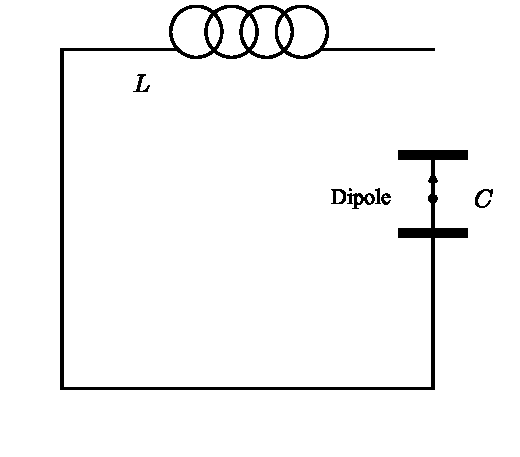
\includegraphics[width=0.72\textwidth]{fig_2.2.pdf}
\caption*{图 2.2\quad 电容器中含偶极子的 CL 电路。}
\end{figure}

\subsection*{问题 2.2.1}

证明式 (2.2.14)。（提示：计算 $\int\prod_i\mathrm{d}x_i\,\mathrm{e}^{J_ix_i}\mathrm{e}^{-\frac{1}{2}x_i\Lambda_{ij}x_j}$，并把结果展开到 $J$ 的二阶。）

\subsection*{问题 2.2.2}

\begin{enumerate}
\item[(a)] 用相干态路径积分和生成泛函 $\frac{Z[\eta(t),\bar{\eta}(t)]}{Z[0,0]}$，其中
\begin{equation*}
Z[\eta(t),\bar{\eta}(t)]=\int\mathcal{D}^2[a(t)]\,\mathrm{e}^{\mathrm{i}\int\mathrm{d}t\,\left[\mathrm{i}\frac{1}{2}\left(a^*\frac{\mathrm{d}}{\mathrm{d}t}a-a\frac{\mathrm{d}}{\mathrm{d}t}a^*\right)-\omega_0a^*a-\bar{\eta}a-\eta a^*\right]}
\end{equation*}
计算实空间与频率空间中的关联 $\mathrm{i}G(t)=\langle a(t)a^*(0)\rangle$。（提示：用复时间 $t\to t\mathrm{e}^{-\mathrm{i}0^+}$。）
\item[(b)] 在 $t>0$ 与 $t<0$ 两种情形下，把你的结果与相应的编时关联函数 $\langle 0|T(\hat{a}(t)\hat{a}^\dagger(0))|0\rangle$ 进行比较。并注意 $t\to 0^\pm$ 的极限。
\item[(c)] 现在我们想用相干态路径积分计算 $\langle 0|\hat{a}^\dagger\hat{a}|0\rangle$ 和 $\langle 0|\hat{a}\hat{a}^\dagger|0\rangle$。问题在于，在路径积分中这两个算符都变成了 $a^*a$。结合上述计算，我们该如何解决这一问题？请描述如何用路径积分计算如下关联：$\langle 0|(\hat{a}\hat{a}^\dagger)_{t_1}(\hat{a}\hat{a}^\dagger)_{t_2}|0\rangle$。
\end{enumerate}

\subsection{有效理论}

\begin{keypoints}
\item 有效理论是一个非常重要的概念。如果你只想记住场论中的一件事，那就记住有效理论。
\end{keypoints}

我们知道，电偶极矩与电场 $\mathcal{E}$ 耦合。为考察这种耦合如何影响电场的动力学，让我们考虑一个 CL 电路（见图 2.2）。在没有偶极矩时，电容器中电场的动力学由作用量 $S_0(\mathcal{E})=\int\mathrm{d}t\,\frac{1}{2g}(\dot{\mathcal{E}}^2-\omega_{CL}^2\mathcal{E}^2)$ 描写，其中 $\omega_{CL}$ 是 CL 电路的振荡频率。耦合系统由下式描写：
\begin{equation*}
Z=\int\mathcal{D}x\,\mathcal{D}\mathcal{E}\,\mathrm{e}^{\mathrm{i}S_0(\mathcal{E})+\mathrm{i}\int\mathrm{d}t\,[L(x,\dot{x})+ex\mathcal{E}]}
\end{equation*}
其中 $L(x,\dot{x})$ 描写偶极子的动力学，而 $ex\mathcal{E}$ 描写偶极子与电场之间的耦合。

让我们假设 $\omega_0\gg\omega_{CL}$，并积掉高频运动 $x(t)$。我们得到只含 $\mathcal{E}(t)$ 的路径积分：
\begin{equation*}
\begin{gathered}
Z=\int\mathcal{D}\mathcal{E}\,\mathrm{e}^{\mathrm{i}S_0(\mathcal{E})+\mathrm{i}S_I(\mathcal{E})},\\
\mathrm{e}^{\mathrm{i}S_I}=\frac{Z[\mathcal{E}]}{Z[0]},\qquad Z[\mathcal{E}]=\int\mathcal{D}x\,\mathrm{e}^{\mathrm{i}\int\mathrm{d}t\,\left[\frac{m}{2}\dot{x}^2-\frac{m\omega_0^2}{2}x^2+ex\mathcal{E}\right]}
\end{gathered}
\end{equation*}
我们看到，耦合系统的电场动力学由一个新的作用量 $S_{eff}=S_0+S_I$ 描写，我们称之为有效作用量。完成高斯积分后，我们得到
\begin{align*}
S_I&=\int\mathrm{d}t\,\frac{1}{2m}\mathcal{E}(t)\left(\left(\frac{\mathrm{d}}{\mathrm{d}t}\right)^2+\omega_0^2\right)^{-1}\mathcal{E}(t)\nonumber\\
&=-\int\mathrm{d}t\,\mathrm{d}t'\,\frac{e^2}{2}\mathcal{E}(t)G_x(t-t')\mathcal{E}(t')=-\int\frac{\mathrm{d}\omega}{2\pi}\,\frac{e^2}{2}\mathcal{E}_{-\omega}G_x(\omega)\mathcal{E}_\omega
\end{align*}
这进而给出电场的有效拉格朗日量：
\begin{equation*}
L_{\mathrm{eff}}=\frac{1}{2g}(\dot{\mathcal{E}}^2-\omega_{CL}^2\mathcal{E}^2)+\frac{e^2}{2m}\mathcal{E}\left(\left(\frac{\mathrm{d}}{\mathrm{d}t}\right)^2+\omega_0^2\right)^{-1}\mathcal{E}.
\end{equation*}
在 $\omega_0\gg\omega_{CL}$ 的极限下，$L_{\mathrm{eff}}$ 可以简化为
\begin{equation*}
L_{\mathrm{eff}}=\frac{1}{2g}(\dot{\mathcal{E}}^2-(\omega_{CL}^*)^2\mathcal{E}^2),\qquad \omega_{CL}^*=\sqrt{\omega_{CL}^2-\frac{ge^2}{m\omega_0^2}}.
\end{equation*}
我们看到，积掉高频的 $x(t)$ 之后，低频电场由一个简单的有效拉格朗日量描写。与偶极子的耦合把电场的振荡频率移到了一个较低的值 $\omega_{CL}^*$。

\subsection*{问题 2.2.3}

\textbf{两个耦合谐振子的低能有效理论：}考虑一个由两个耦合谐振子组成的系统：
\begin{equation*}
Z=\int\mathcal{D}x\,\mathcal{D}X\,\mathrm{e}^{\mathrm{i}\int\mathrm{d}t\,L(x,X)}
\end{equation*}
其中
\begin{equation*}
L(x,X)=\frac{1}{2}m\dot{x}^2-\frac{1}{2}m\omega^2x^2+\frac{1}{2}M\dot{X}^2-\frac{1}{2}M\Omega^2X^2-gxX
\end{equation*}
这里我们假设 $\Omega\gg\omega$、$g\sim m\omega^2$ 且 $m\sim M$。此时 $X$ 是一个围绕 $X=0$ 振荡的高能自由度。试通过积掉 $X$，求出描写软自由度 $x$ 的低能动力学的低能有效理论 $L_{\mathrm{eff}}(x)$。（至少应包含领头的 $\frac{1}{\Omega}$ 修正。）特别地，求出有效质量 $m^*$ 和有效弹簧常数 $m^*(\omega^*)^2$。

\subsection{含时响应与耗散}

\begin{keypoints}
\item 响应函数给出响应率的正确实部和虚部，而编时关联函数只给出响应率的正确实部。
\end{keypoints}

我们也可以用路径积分计算对含时电场的响应。注意到 $t$ 时刻的平均偶极矩可以表示为
\begin{equation*}
\begin{aligned}
d(t)=\langle ex(t)\rangle&=e\,\frac{\int\mathcal{D}x\,x(t)\,\mathrm{e}^{\mathrm{i}\int\mathrm{d}t'\,[L(x,\dot{x})+ex\mathcal{E}]}}{\int\mathcal{D}x\,\mathrm{e}^{\mathrm{i}\int\mathrm{d}t'\,[L(x,\dot{x})+ex\mathcal{E}]}}\\
&=-\int_{-\infty}^{+\infty}\mathrm{d}t'\,e^2G_x(t-t')\mathcal{E}(t')+O(\mathcal{E}^2)
\end{aligned}
\end{equation*}
其中
\begin{equation*}
\mathrm{i}G_x(t_1-t_2)=\frac{\int\mathcal{D}x\,x(t_1)x(t_2)\,\mathrm{e}^{\mathrm{i}\int\mathrm{d}t\,L(x,\dot{x})}}{\int\mathcal{D}x\,\mathrm{e}^{\mathrm{i}\int\mathrm{d}t'\,L(x,\dot{x})}}
\end{equation*}
在频率空间中，上式变为 $d_\omega=-e^2G_x(\omega)E_\omega$。我们求得有限频率响应率 $\chi(\omega)$ 为
\begin{equation*}
\chi(\omega)=-e^2G_x(\omega)=-\frac{e^2m^{-1}}{\omega^2-\omega_0^2+\mathrm{i}0^+}\tag{2.2.20}
\end{equation*}
虚部 $\mathrm{i}0^+$ 已在 2.2.2 节中算出。

上述对有限频率响应率的路径积分计算属于一类被称为“形式计算”的计算。用路径积分我们可以“形式地”计算很多东西。然而，对“形式”计算得到的结果必须持保留态度。这些结果通常或多或少是正确的，但未必完全正确。正如我们将在 2.4.3 节看到的，$\mathrm{Im}\chi(\omega)\omega$ 有其物理意义：它代表频率 $\omega$ 处的摩擦系数。由于 $\mathrm{Im}G(\omega)$ 总是负的，我们发现当 $\omega>0$ 时 $\mathrm{Im}\chi(\omega)\omega>0$，而当 $\omega<0$ 时 $\mathrm{Im}\chi(\omega)\omega<0$。$\omega<0$ 时摩擦系数为负是一个非物理且错误的结果。因此，式 (2.2.20) 并不完全正确，它与先前的结果 (2.2.8) 不一致。

事实上，只要把编时关联 $G_x$ 换成响应函数 $D$，就能从这个错误的结果得到正确的结果 (2.2.8)：
\begin{equation*}
d(t)=-\int_{-\infty}^{+\infty}\mathrm{d}t'\,e^2D(t-t')\mathcal{E}(t')+O(\mathcal{E}^2)
\end{equation*}
\begin{equation*}
\chi(\omega)=-e^2D(\omega)=-\frac{e^2m^{-1}}{\omega^2-\omega_0^2+\mathrm{i}\,\mathrm{sgn}(\omega)0^+}
\end{equation*}
此时，$\mathrm{Im}\chi(\omega)\omega$ 总是正的。

% 新增术语（本块新增，供术语表维护者收录）：
% response function -> 响应函数
% time-ordered correlation function -> 编时关联函数
% time-ordering operator -> 编时算符
% effective action -> 有效作用量
% effective Lagrangian -> 有效拉格朗日量
% Gaussian integral -> 高斯积分
% CL circuit -> CL 电路
% capacitor -> 电容器
% dipole moment -> 偶极矩
% Heisenberg picture -> 海森堡绘景
% formal calculation -> 形式计算
% friction coefficient -> 摩擦系数
% spring constant -> 弹簧常数

在上面的路径积分计算中，我们犯了一个错误：把路径积分平均 $\frac{\int \mathcal{D}x\, x(t)\mathrm{e}^{\mathrm{i}S}}{\int \mathcal{D}x\, \mathrm{e}^{\mathrm{i}S}}$ 与量子力学平均 $\langle\psi(t)|x|\psi(t)\rangle$ 混为一谈。要使路径积分计算有效，我们需要假定在电场存在时这两种平均是相同的。也就是说，
\begin{equation*}
\langle 0|U^{\dagger}(t,-\infty)\, x\, U(t,-\infty)|0\rangle = \frac{\langle 0|U(\infty,t)\, x\, U(t,-\infty)|0\rangle}{\langle 0|U(\infty,-\infty)|0\rangle} \tag{2.2.21}
\end{equation*}
其中右端是路径积分平均，左端是量子力学平均。只有当我们缓慢地开启再关闭电场，使得基态 $|0\rangle$ 从 $t=-\infty$ 到 $t=\infty$ 演化回同一个基态时，这一假定才是正确的：
\begin{equation*}
|0\rangle = \mathrm{e}^{\mathrm{i}\theta} U(\infty,-\infty)|0\rangle \tag{2.2.22}
\end{equation*}
在这种情况下，
\begin{equation*}
\langle 0|U^{\dagger}(t,-\infty) = \langle 0|U(-\infty,\infty)U(\infty,t) = \mathrm{e}^{\mathrm{i}\theta}\langle 0|U(\infty,t)
\end{equation*}
于是我们看到，式 (2.2.21) 在条件 (2.2.22) 之下确实成立。然而，若 $\mathcal{E}(t)$ 变化迅速，把振子激发到越来越高的激发态，那么式 (2.2.22) 将不再正确，而且更糟的是，当存在耗散时 $\langle 0|U(\infty,-\infty)|0\rangle$ 可能会变为零。

这里我们学到了两点。其一，在存在耗散时路径积分的结果可能不正确；其二，这个毛病可以用响应函数替换编时关联函数来纠正。

\subsection*{问题 2.2.4}

考虑一个谐振子。计算（编时）流关联函数 $\mathrm{i}G_j(t) = \langle j(t)j(0)\rangle$ 在频率空间中的形式，即 $G_j(\omega) = \int \mathrm{d}t\, G_j(t)\mathrm{e}^{\mathrm{i}\omega t}$，其中流算符为 $j = e\dot{x}$。利用（比如说）经典物理计算有限频率电导 $\sigma(\omega)$（定义为 $j(\omega) = \sigma(\omega)E_{\omega}$）。（你可以加入少量摩擦以得到耗散项。）证明：对 $\omega > 0$，$\sigma(\omega)$ 具有形式 $\sigma(\omega) = C\frac{G_j(\omega)}{\omega}$，并求出系数 $C$。证明：$\sigma(\omega)$ 仅在 $\omega = \omega_0$ 处才有非零实部。（提示：保留 $G_j$ 中的 $\mathrm{i}0^{+}$ 项。）在这个频率上，振子可以通过跃迁到较高的激发态来吸收能量。我们看到，要有有限的实直流电导，就需要有无能隙激发。

\subsection{有限温度下的关联函数}

在有限温度下，线性响应是所有激发态的响应以玻尔兹曼因子（Boltzmann factor）加权后的平均。由于态 $|\psi_n\rangle$ 的响应函数由式 (2.2.4) 给出，有限温度响应函数即为
\begin{equation*}
D^{\beta}(t-t') = \sum_n -\mathrm{i}\,\Theta(t-t')\,\langle\psi_n|[O_2(t), O_1(t')]\,|\psi_n\rangle\, \frac{\mathrm{e}^{-\epsilon_n/T}}{Z}
\end{equation*}
我们再次看到，线性响应可以由相应的关联函数来描述。在频率空间中，
\begin{equation*}
\langle O_2\rangle_{\omega} = D^{\beta}_{\omega} f_{\omega}
\end{equation*}
对有限温度成立。于是，
\begin{equation*}
D^{\beta}_{\omega} = \int \mathrm{d}t\, D^{\beta}(t)\,\mathrm{e}^{\mathrm{i}t\omega}
\end{equation*}
可以视为有限温度下的有限频率响应率。

类似地，我们定义编时的有限温度关联函数
\begin{equation*}
\mathrm{i}G^{\beta}(t) = \sum_n \langle\psi_n|T(O_2(t)O_1(0))|\psi_n\rangle\, \frac{\mathrm{e}^{-\epsilon_n\beta}}{Z}
\end{equation*}
有了这个定义，式 (2.2.18) 可以推广到有限温度：
\begin{equation*}
D^{\beta}(t) = 2\Theta(t)\operatorname{Re} G^{\beta}(t) \tag{2.2.23}
\end{equation*}

\subsection{关联函数之间的关系}

\begin{keypoints}
\item 有限温度下的响应函数、编时关联函数和谱函数（spectral function），都可以通过适当的解析延拓由有限温度虚时关联函数计算出来。
\end{keypoints}

我们已经引入了好几种关联函数。响应函数与线性响应实验中所测量的各种响应率直接相关；编时关联函数则容易用路径积分计算。本节我们将讨论这些关联函数之间的关系。这些关系使我们能够由编时关联函数得到响应函数。本节中的计算相当形式化，但结果是有用的。如果你不喜欢形式计算，可以跳过本节；你只需知道方框公式中的那些关系即可。

首先，我们来研究两个算符 $O_1$ 与 $O_2$ 的有限温度关联在实时与虚时之间的关系：$\mathrm{i}G^{\beta}(t) = \langle T[O_2(t)O_1(0)]\rangle$ 与 $\mathcal{G}^{\beta}(\tau) = \langle T_{\tau}[O_2(\tau)O_1(0)]\rangle$。为了得到稍后用于费米子系统的更普遍的结果，我们把 $G^{\beta}(t)$ 与 $\mathcal{G}^{\beta}(\tau)$ 的定义推广如下：
\begin{align*}
\mathrm{i}G^{\beta}(t)\bigr|_{t>0} &= \langle O_2(t)O_1(0)\rangle
& \mathrm{i}G^{\beta}(t)\bigr|_{t<0} &= \eta\,\langle O_1(0)O_2(t)\rangle
\\
\mathcal{G}^{\beta}(\tau)\bigr|_{\tau>0} &= \langle O_2(\tau)O_1(0)\rangle
& \mathcal{G}^{\beta}(\tau)\bigr|_{\tau<0} &= \eta\,\langle O_1(0)O_2(\tau)\rangle
\end{align*}
其中 $\eta = \pm$。当 $\eta = +$ 时，这些关联称为玻色型的；当 $\eta = -$ 时，称为费米型的。注意这里我们并不假定 $O_{1,2} = O^{\dagger}_{1,2}$。利用
\begin{align*}
\langle\psi_n|O_2(t)O_1(0)|\psi_n\rangle &= \frac{\langle\psi_n|O_2\, U(t,0)\, O_1|\psi_n\rangle}{\langle\psi_n|U(t,0)|\psi_n\rangle}
\\
&= \sum_m \langle\psi_n|O_2|\psi_m\rangle\langle\psi_m|O_1|\psi_n\rangle\, \mathrm{e}^{-\mathrm{i}(\epsilon_m - \epsilon_n)t}
\end{align*}
我们求得 $G^{\beta}(t)$ 的谱表示为
\begin{align*}
\mathrm{i}G^{\beta}(t)\bigr|_{t>0} &= \sum_{m,n} \langle\psi_n|O_2|\psi_m\rangle\langle\psi_m|O_1|\psi_n\rangle\, \frac{\mathrm{e}^{-\epsilon_n\beta - \mathrm{i}(\epsilon_m - \epsilon_n)t}}{Z}
\\
\mathrm{i}G^{\beta}(t)\bigr|_{t<0} &= \eta \sum_{m,n} \langle\psi_n|O_1|\psi_m\rangle\langle\psi_m|O_2|\psi_n\rangle\, \frac{\mathrm{e}^{-\epsilon_n\beta + \mathrm{i}(\epsilon_m - \epsilon_n)t}}{Z} \tag{2.2.24}
\end{align*}
如果我们如下引入有限温度谱函数：
\begin{align*}
A^{\beta}_{+}(\nu) &= \sum_{m,n} \delta[\nu - (\epsilon_m - \epsilon_n)]\, \langle\psi_n|O_2|\psi_m\rangle\langle\psi_m|O_1|\psi_n\rangle\, \frac{\mathrm{e}^{-\epsilon_n\beta}}{Z}
\\
A^{\beta}_{-}(\nu) &= \sum_{m,n} \delta[\nu + (\epsilon_m - \epsilon_n)]\, \langle\psi_n|O_1|\psi_m\rangle\langle\psi_m|O_2|\psi_n\rangle\, \frac{\mathrm{e}^{-\epsilon_n\beta}}{Z}
\end{align*}
便可把 $G^{\beta}$ 改写为
\begin{equation*}
\mathrm{i}G^{\beta}(t)\bigr|_{t>0} = \int \mathrm{d}\nu\, A^{\beta}_{+}(\nu)\,\mathrm{e}^{-\mathrm{i}\nu t}, \qquad \mathrm{i}G^{\beta}(t)\bigr|_{t<0} = \eta \int \mathrm{d}\nu\, A^{\beta}_{-}(\nu)\,\mathrm{e}^{-\mathrm{i}\nu t} \tag{2.2.25}
\end{equation*}

为理解谱函数的含义，我们来考虑零温谱函数 $A_{+}(\nu) \allowbreak= \sum_m \delta[\nu - (\epsilon_m - \epsilon_0)]\allowbreak\langle 0|O_2|\psi_m\rangle\allowbreak\langle\psi_m|O_1|0\rangle$。我们看到，当 $O_1$ 与 $O_2$ 作用在基态 $|0\rangle$ 上时，它们产生激发态 $O_1|0\rangle = \sum_m C_{1,m}|\psi_m\rangle$ 与 $O_2|0\rangle = \sum_m C_{2,m}|\psi_m\rangle$，振幅分别为 $C_{1,m}$ 与 $C_{2,m}$。函数 $A_{+}(\nu)$ 恰是 $C_{1,m}$ 与 $C_{2,m}$ 的乘积：$A_{+}(\nu) = \sum_m \delta[\nu - (\epsilon_m - \epsilon_0)]\, C^{\dagger}_{2,m}C_{1,m}$。若 $A_{+}(\nu) \neq 0$，则一个能量为 $\epsilon_0 + \nu$ 的激发态同时被 $O_1$ 和 $O_2$ 产生。当 $O_1 = O_2$ 时，$A_{+}(\nu)$ 就是 $O_1$ 所产生的能量为 $\nu$ 的诸态的权重。

我们注意，有限温度谱函数可以改写为
\begin{align*}
A^{\beta}_{+}(\omega) &= \sum_{m,n} \langle\psi_n|O_2|\psi_m\rangle\langle\psi_m|O_1|\psi_n\rangle\, \frac{\mathrm{e}^{-\epsilon_n\beta}}{Z}\, \delta\bigl(\omega - (\epsilon_m - \epsilon_n)\bigr)
\\
&= \mathrm{e}^{\beta\omega/2} \sum_{m,n} \langle\psi_n|O_2|\psi_m\rangle\langle\psi_m|O_1|\psi_n\rangle\, \frac{\mathrm{e}^{-(\epsilon_m + \epsilon_n)\beta/2}}{Z}\, \delta\bigl(\omega - (\epsilon_m - \epsilon_n)\bigr) \tag{2.2.26}
\end{align*}
\begin{align*}
A^{\beta}_{-}(\omega) &= \sum_{m,n} \langle\psi_n|O_1|\psi_m\rangle\langle\psi_m|O_2|\psi_n\rangle\, \frac{\mathrm{e}^{-\epsilon_n\beta}}{Z}\, \delta\bigl(\omega + (\epsilon_m - \epsilon_n)\bigr) \tag{2.2.27}
\\
&= \mathrm{e}^{-\beta\omega/2} \sum_{m,n} \langle\psi_n|O_1|\psi_m\rangle\langle\psi_m|O_2|\psi_n\rangle\, \frac{\mathrm{e}^{-(\epsilon_m + \epsilon_n)\beta/2}}{Z}\, \delta\bigl(\omega + (\epsilon_m - \epsilon_n)\bigr)
\\
&= \mathrm{e}^{-\beta\omega/2} \sum_{m,n} \langle\psi_n|O_2|\psi_m\rangle\langle\psi_m|O_1|\psi_n\rangle\, \frac{\mathrm{e}^{-(\epsilon_m + \epsilon_n)\beta/2}}{Z}\, \delta\bigl(\omega - (\epsilon_m - \epsilon_n)\bigr)
\end{align*}
在式 (2.2.27) 的最后一行中我们交换了 $m$ 与 $n$。在这种形式下，可以看出有限温度下 $A^{\beta}_{+}$ 与 $A^{\beta}_{-}$ 之间一个非常简单的关系：
\begin{equation*}
\boxed{\; A^{\beta}_{+}(\omega) = \mathrm{e}^{\beta\omega} A^{\beta}_{-}(\omega) \;} \tag{2.2.28}
\end{equation*}
我们还注意，当 $\omega \lesssim -T$ 时 $A^{\beta}_{+}$ 几乎为零，而当 $\omega \gtrsim -T$ 时 $A^{\beta}_{-}$ 几乎为零。在零温下，我们有
\begin{equation*}
A_{+}(\omega < 0) = 0, \qquad A_{-}(\omega > 0) = 0
\end{equation*}
为了在频率空间中把 $G^{\beta}$ 的谱函数 $A^{\beta}_{\pm}$ 联系起来，我们需要引入
\begin{equation*}
G^{\beta}_{+}(t) = \Theta(t)G^{\beta}(t), \qquad G^{\beta}_{-}(t) = \Theta(-t)G^{\beta}(t)
\end{equation*}
在频率空间中，我们有
\begin{align*}
G^{\beta}_{+}(\omega) &= \sum_{m,n} \frac{\langle\psi_n|O_2|\psi_m\rangle\langle\psi_m|O_1|\psi_n\rangle}{\omega - (\epsilon_m - \epsilon_n) + \mathrm{i}0^{+}}\, \frac{\mathrm{e}^{-\epsilon_n\beta}}{Z}
\\
G^{\beta}_{-}(\omega) &= \eta \sum_{m,n} \frac{\langle\psi_n|O_1|\psi_m\rangle\langle\psi_m|O_2|\psi_n\rangle}{-\omega - (\epsilon_m - \epsilon_n) + \mathrm{i}0^{+}}\, \frac{\mathrm{e}^{-\epsilon_n\beta}}{Z}
\end{align*}
我们发现
\begin{equation*}
\boxed{\; G^{\beta}_{+}(\omega) = \int \mathrm{d}\nu\, \frac{A^{\beta}_{+}(\nu)}{\omega - \nu + \mathrm{i}0^{+}} \qquad G^{\beta}_{-}(\omega) = -\eta \int \mathrm{d}\nu\, \frac{A^{\beta}_{-}(\nu)}{\omega - \nu - \mathrm{i}0^{+}} \;} \tag{2.2.29}
\end{equation*}
以及 $G^{\beta}(\omega) = G^{\beta}_{+}(\omega) + G^{\beta}_{-}(\omega)$。

接下来，我们考虑响应函数 $D^{\beta}(t)$，把它推广为
\begin{equation*}
D^{\beta}(t-t') = \sum_n -\mathrm{i}\,\Theta(t-t')\,\langle\psi_n|O_2(t)O_1(t') - \eta\, O_1(t')O_2(t)\,|\psi_n\rangle\, \frac{\mathrm{e}^{-\epsilon_n/T}}{Z} \tag{2.2.30}
\end{equation*}
它有如下谱展开：
\begin{align*}
D^{\beta}(\omega) &= \sum_{m,n} \frac{\langle\psi_n|O_2|\psi_m\rangle\langle\psi_m|O_1|\psi_n\rangle}{\omega - (\epsilon_m - \epsilon_n) + \mathrm{i}0^{+}}\, \frac{\mathrm{e}^{-\epsilon_n\beta}}{Z}
\\
&\quad + \eta \sum_{m,n} \frac{\langle\psi_n|O_1|\psi_m\rangle\langle\psi_m|O_2|\psi_n\rangle}{-\omega - (\epsilon_m - \epsilon_n) - \mathrm{i}0^{+}}\, \frac{\mathrm{e}^{-\epsilon_n\beta}}{Z} \tag{2.2.31}
\end{align*}
我们发现
\begin{equation*}
\boxed{\; D^{\beta}(\omega) = \int \mathrm{d}\nu\, \frac{A^{\beta}_{+}(\nu)}{\omega - \nu + \mathrm{i}0^{+}} - \eta \int \mathrm{d}\nu\, \frac{A^{\beta}_{-}(\nu)}{\omega - \nu + \mathrm{i}0^{+}} \;} \tag{2.2.32}
\end{equation*}
我们看到，由谱函数 $A^{\beta}_{\pm}$ 可以同时确定编时关联函数 $G^{\beta}$ 与响应函数 $D^{\beta}$。

从路径积分出发计算谱函数的一个办法，是使用编时的虚时关联函数
\begin{equation*}
\mathcal{G}^{\beta}(\tau_2, \tau_1) = Z^{-1}\operatorname{Tr}\left( T_{\tau}(O_2(\tau_2)O_1(\tau_1))\, \mathrm{e}^{-\beta H} \right)
\end{equation*}
其中 $0 < \tau_{1,2} < \beta$。函数 $\mathcal{G}^{\beta}(\tau_2, \tau_1)$ 也可以写为
\begin{equation*}
\mathcal{G}^{\beta}(\tau_2, \tau_1) =
\begin{cases}
\dfrac{\operatorname{Tr}\bigl(\mathrm{e}^{-(\beta - \tau_2)H}\, O_2\, \mathrm{e}^{-(\tau_2 - \tau_1)H}\, O_1\, \mathrm{e}^{-\tau_1 H}\bigr)}{\operatorname{Tr}(\mathrm{e}^{-\beta H})}, & \tau_2 > \tau_1 \\[3ex]
\eta\, \dfrac{\operatorname{Tr}\bigl(\mathrm{e}^{-(\beta - \tau_1)H}\, O_1\, \mathrm{e}^{-(\tau_1 - \tau_2)H}\, O_2\, \mathrm{e}^{-\tau_2 H}\bigr)}{\operatorname{Tr}(\mathrm{e}^{-\beta H})}, & \tau_1 > \tau_2
\end{cases}
\end{equation*}
由此可以证明
\begin{equation*}
\mathcal{G}^{\beta}(\tau_2, \tau_1) = \mathcal{G}^{\beta}(\tau_2 - \tau_1, 0) \equiv \mathcal{G}^{\beta}(\tau_2 - \tau_1), \qquad \mathcal{G}^{\beta}(\tau) = \eta\, \mathcal{G}^{\beta}(\tau + \beta)
\end{equation*}
函数 $\mathcal{G}^{\beta}(\tau)$ 也有谱表示。对 $0 < \tau < \beta$，我们有
\begin{equation*}
\mathcal{G}^{\beta}(\tau) =
\begin{cases}
\sum\limits_{m,n} \langle\psi_n|O_2|\psi_m\rangle\langle\psi_m|O_1|\psi_n\rangle\, \dfrac{\mathrm{e}^{-\epsilon_n\beta - (\epsilon_m - \epsilon_n)\tau}}{Z}, & \tau > 0 \\[3ex]
\eta \sum\limits_{m,n} \langle\psi_n|O_1|\psi_m\rangle\langle\psi_m|O_2|\psi_n\rangle\, \dfrac{\mathrm{e}^{-\epsilon_n\beta + (\epsilon_m - \epsilon_n)\tau}}{Z}, & \tau < 0
\end{cases} \tag{2.2.33}
\end{equation*}
比较式 (2.2.24) 与式 (2.2.33)，我们看到 $G^{\beta}$ 与 $\mathcal{G}^{\beta}$ 之间有如下关系：
\begin{equation*}
\boxed{\; \mathrm{i}G^{\beta}(t) = \mathcal{G}^{\beta}\bigl(\mathrm{i}t + \mathrm{sgn}(t)0^{+}\bigr) \;} \tag{2.2.34}
\end{equation*}
即使在有限温度下，实时格林函数也可以由虚时格林函数算出。

由于 $\mathcal{G}^{\beta}(\tau)$ 是（反）周期的，其频率是离散的：$\eta = +$ 时 $\omega_l = 2\pi T \times$ 整数，$\eta = -$ 时 $\omega_l = 2\pi T \times (\text{整数} + \frac{1}{2})$。在频率空间中，我们天真地得到
\begin{align*}
\mathcal{G}^{\beta}(\omega_l) &= \int_0^{\beta} \mathrm{d}\tau\, \mathcal{G}^{\beta}(\tau)\, \mathrm{e}^{\mathrm{i}\omega_l \tau}
\\
&= -\sum_{m,n} \frac{\langle\psi_n|O_2|\psi_m\rangle\langle\psi_m|O_1|\psi_n\rangle}{\mathrm{i}\omega_l - \epsilon_m + \epsilon_n}\, \frac{\mathrm{e}^{-\epsilon_n\beta} - \eta\,\mathrm{e}^{-\epsilon_m\beta}}{Z}
\end{align*}
然而，当 $\eta = 1$ 且 $\omega_l = 0$ 时，$m = n$ 的那些项没有定义。这些项应当是 $\langle\psi_n|O_2|\psi_n\rangle\allowbreak\langle\psi_n|O_1|\psi_n\rangle \beta\allowbreak\, \mathrm{e}^{-\epsilon_n\beta}/Z$。所以，严格地说，我们有
\begin{align*}
\mathcal{G}^{\beta}(\omega_l) &= -\sum_{m,n} \frac{\langle\psi_n|O_2|\psi_m\rangle\langle\psi_m|O_1|\psi_n\rangle}{\mathrm{i}\omega_l - \epsilon_m + \epsilon_n + T\delta}\, \frac{\mathrm{e}^{-\epsilon_n\beta} - (\eta + \delta)\,\mathrm{e}^{-\epsilon_m\beta}}{Z} \tag{2.2.35}
\\
&= -\sum_{m,n} \left( \frac{\langle\psi_n|O_2|\psi_m\rangle\langle\psi_m|O_1|\psi_n\rangle}{\mathrm{i}\omega_l - (\epsilon_m - \epsilon_n) + T\delta} + (\eta + \delta)\, \frac{\langle\psi_n|O_1|\psi_m\rangle\langle\psi_m|O_2|\psi_n\rangle}{-\mathrm{i}\omega_l - (\epsilon_m - \epsilon_n) - T\delta} \right) \frac{\mathrm{e}^{-\epsilon_n\beta}}{Z}
\end{align*}
其中 $\delta$ 是一个小的复数。这使我们能够得到，对 $\omega \neq 0$，
\begin{align*}
&\frac{1}{2\mathrm{i}}\left[ \mathcal{G}^{\beta}(\mathrm{i}\omega_l \to \omega + \mathrm{i}0^{+}) - \mathcal{G}^{\beta}(\mathrm{i}\omega_l \to \omega - \mathrm{i}0^{+}) \right] \tag{2.2.36}
\\
&\quad = \bigl(\mathrm{e}^{\beta\omega/2} - \eta\,\mathrm{e}^{-\beta\omega/2}\bigr) \sum_{m,n} \langle\psi_n|O_2|\psi_m\rangle\langle\psi_m|O_1|\psi_n\rangle\, \frac{\mathrm{e}^{-(\epsilon_m + \epsilon_n)\beta/2}}{Z}\, \pi\delta\bigl(\omega - (\epsilon_m - \epsilon_n)\bigr).
\end{align*}
注意，当 $\omega \neq 0$ 时 $\delta$ 不起作用，可以略去。最后，把式 (2.2.36) 与式 (2.2.26)、式 (2.2.27) 相比较，便能借助 $\mathcal{G}^{\beta}(\omega_l)$ 表示 $A^{\beta}_{\pm}$。对 $\omega \neq 0$，我们有
\begin{equation*}
\boxed{
\begin{aligned}
A^{\beta}_{+}(\omega) &= [1 + \eta\, n_{\eta}(\omega)]\,(\pi)^{-1} \frac{1}{2\mathrm{i}}\left[ \mathcal{G}^{\beta}(\mathrm{i}\omega_l \to \omega + \mathrm{i}0^{+}) - \mathcal{G}^{\beta}(\mathrm{i}\omega_l \to \omega - \mathrm{i}0^{+}) \right]
\\
A^{\beta}_{-}(\omega) &= n_{\eta}(\omega)\,(\pi)^{-1} \frac{1}{2\mathrm{i}}\left[ \mathcal{G}^{\beta}(\mathrm{i}\omega_l \to \omega + \mathrm{i}0^{+}) - \mathcal{G}^{\beta}(\mathrm{i}\omega_l \to \omega - \mathrm{i}0^{+}) \right]
\end{aligned}
} \tag{2.2.37}
\end{equation*}
其中 $n_{+}(\omega) = n_B(\omega) = \frac{1}{\mathrm{e}^{\beta\omega} - 1}$ 与 $n_{-}(\omega) = n_F(\omega) = \frac{1}{\mathrm{e}^{\beta\omega} + 1}$ 分别是玻色子与费米子的占据数。这样我们便能由 $\mathcal{G}^{\beta}$ 确定 $G^{\beta}$ 与 $D^{\beta}$。特别地，比较式 (2.2.31) 与式 (2.2.35)，我们看到 $D^{\beta}(\omega)$ 与 $\mathcal{G}^{\beta}(\omega_l)$ 之间有一个非常简单的关系：
\begin{equation*}
\boxed{\; D(\omega) = -\mathcal{G}^{\beta}(\omega_l)\bigr|_{\mathrm{i}\omega_l \to \omega + \mathrm{i}0^{+}}, \qquad \text{对 } \omega \neq 0. \;} \tag{2.2.38}
\end{equation*}
同样，由于 $\omega \neq 0$，$\delta$ 已被略去。

有趣的是，$\mathcal{G}^{\beta}(\tau)$ 的傅里叶变换与解析延拓两者不可交换：若先做解析延拓，便得到编时关联函数 $G^{\beta}(t)$；若先做傅里叶变换，便得到响应函数 $D^{\beta}(\omega)$。有人或许想换用另一种解析延拓 $\mathrm{i}\omega_n \to \omega(1 + \mathrm{i}0^{+})$，它其实更为自然。从我们的谱表示可以看出，新的解析延拓仍然无法把 $\mathcal{G}^{\beta}(\omega_n)$ 变成 $G^{\beta}(\omega)$。不过在零温下，我们确实有
\begin{equation*}
\boxed{\; G(\omega) = -\mathcal{G}(\omega)\bigr|_{\mathrm{i}\omega \to \omega(1 + \mathrm{i}0^{+})} \;} \tag{2.2.39}
\end{equation*}

以上所有结果都是在非常一般的情形下得到的，其中 $O_{1,2}$ 甚至未必是厄米的。当 $O_1 = O^{\dagger}_1$ 且 $O_2 = O^{\dagger}_2$ 时，结果可以取更简单的形式。在 $T = 0$ 且 $\omega \neq 0$ 时，我们有
\begin{equation*}
\boxed{
\begin{aligned}
D(t) &= 2\Theta(t)\operatorname{Re} G(t), & \mathrm{i}G(t) &= \mathcal{G}\bigl(\mathrm{i}t + \mathrm{sgn}(t)0^{+}\bigr)
\\
D(\omega) &= \operatorname{Re} G(\omega) + \mathrm{i}\,\mathrm{sgn}(\omega)\operatorname{Im} G(\omega), & D(\omega) &= -\mathcal{G}(\omega)\bigr|_{\mathrm{i}\omega \to \omega + \mathrm{i}0^{+}}
\end{aligned}
} \tag{2.2.40}
\end{equation*}
对 $T \neq 0$ 且 $\omega \neq 0$，我们有
\begin{equation*}
\boxed{
\begin{aligned}
D^{\beta}(t) &= 2\Theta(t)\operatorname{Re} G^{\beta}(t), & \mathrm{i}G^{\beta}(t) &= \mathcal{G}^{\beta}\bigl(\mathrm{i}t + \mathrm{sgn}(t)0^{+}\bigr)
\\
D^{\beta}(\omega) &= G^{\beta}_{+}(\omega) + \left( G^{\beta}_{+}(-\omega) \right)^{*}, & D^{\beta}(\omega) &= -\mathcal{G}^{\beta}(\omega_l)\bigr|_{\mathrm{i}\omega_l \to \omega + \mathrm{i}0^{+}}
\end{aligned}
} \tag{2.2.41}
\end{equation*}
$D^{\beta}(\omega)$ 与 $G^{\beta}(\omega)$ 之间没有简单的关系。

当 $O_1 = O^{\dagger}_2$ 时，函数 $A^{\beta}_{\pm}$ 是实且正的，并且 $\frac{1}{2\mathrm{i}}\bigl[ \mathcal{G}^{\beta}(\mathrm{i}\omega_l \to \omega + \mathrm{i}0^{+}) - \mathcal{G}^{\beta}(\mathrm{i}\omega_l \to \omega - \mathrm{i}0^{+}) \bigr] = \operatorname{Im} \mathcal{G}^{\beta}(\mathrm{i}\omega_l \to \omega + \mathrm{i}0^{+})$。我们有
\begin{equation*}
\boxed{
\begin{aligned}
A^{\beta}_{+}(\omega) &= [1 + \eta\, n_{\eta}(\omega)]\,(\pi)^{-1} \operatorname{Im} \mathcal{G}^{\beta}(\mathrm{i}\omega_l \to \omega + \mathrm{i}0^{+})
\\
&= -[1 + \eta\, n_{\eta}(\omega)]\,(\pi)^{-1} \operatorname{Im} D^{\beta}(\omega)
\\
&= -\frac{1}{1 + \eta\,\mathrm{e}^{-\beta\omega}}\,(\pi)^{-1} \operatorname{Im} G^{\beta}(\omega)
\end{aligned}
} \tag{2.2.42}
\end{equation*}
我们看到，谱函数 $A^{\beta}_{\pm}$ 可以由 $G^{\beta}$、$D^{\beta}$ 或 $\mathcal{G}^{\beta}$ 之一确定，进而确定其余的关联函数。

作为例子，我们来计算振子问题在有限温度下的响应率。在频率空间中，虚时路径积分取如下形式
\begin{equation*}
Z = \int \mathcal{D}[x(\tau)]\; \mathrm{e}^{-\int_0^{\beta} \mathrm{d}\tau\, [\frac{m}{2}\dot{x}^2 + \frac{m\omega_0^2}{2} x^2]} = \int \mathcal{D}x_{\omega}\; \mathrm{e}^{-\frac{1}{2} \sum_{\omega_n = -\infty}^{\infty} x_{-\omega_n}\left[ m\omega_n^2 + m\omega_0^2 \right] x_{\omega_n}}
\end{equation*}
其中 $x_{\omega_n} = \int_0^{\beta} \mathrm{d}\tau\, x(\tau)\beta^{-1/2}\mathrm{e}^{\mathrm{i}\tau\omega_n}$。我们求得
\begin{equation*}
\mathcal{G}^{\beta}_{x}(\omega_n) = \langle x_{\omega_n} x_{-\omega_n} \rangle = \frac{m^{-1}}{\omega_n^2 + \omega_0^2} \tag{2.2.43}
\end{equation*}
于是有限温度响应率为
\begin{equation*}
\chi(\omega) = -D(\omega) = \mathcal{G}^{\beta}_{x}\bigl(-\mathrm{i}(\omega + \mathrm{i}0^{+})\bigr) = \frac{m^{-1}}{\omega_0^2 - \omega^2 - \mathrm{i}\,\mathrm{sgn}(\omega)0^{+}}
\end{equation*}
如预期的那样，它与温度无关。

\subsection*{问题 2.2.5}

用谱表示证明式 (2.2.39)。

\subsection*{问题 2.2.6}

从 $\mathcal{G}^{\beta}(\tau)$ 的定义出发证明式 (2.2.35)。

\subsection*{问题 2.2.7}

证明式 (2.2.43)。计算有限温度下的 $\langle x^2\rangle = \mathcal{G}^{\beta}_{x}(\tau)\bigr|_{\tau = 0}$。检查 $T \to 0$ 与 $T \to \infty$ 极限。（提示：下面的技巧在有限温度计算中经常用到，可能有用：
\begin{figure}[H]
\centering
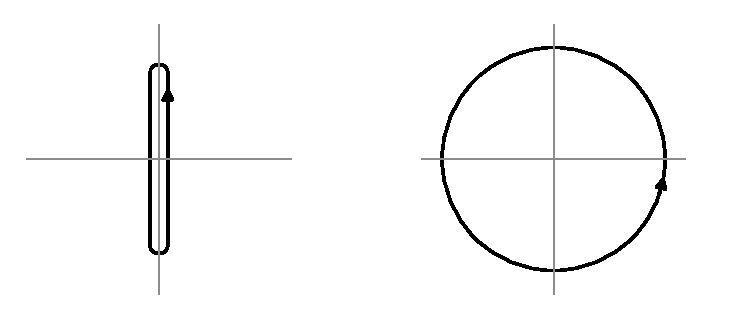
\includegraphics[width=0.72\textwidth]{fig_2.3.pdf}
\caption*{图 2.3\quad 围道 $C_1$ 与 $C_2$。}
\end{figure}
\begin{equation*}
\sum_{n = -\infty}^{\infty} \frac{T}{\omega_n^2 + \omega_0^2} = \oint_{C_1} \frac{\mathrm{d}z}{2\pi\mathrm{i}}\; \frac{1}{(-\mathrm{i}z)^2 + \omega_0^2}\; \frac{1}{\mathrm{e}^{\beta z} - 1}, \qquad \oint_{C_2} \frac{\mathrm{d}z}{2\pi\mathrm{i}}\; \frac{1}{(-\mathrm{i}z)^2 + \omega_0^2}\; \frac{1}{\mathrm{e}^{\beta z} - 1} = 0
\end{equation*}
其中 $C_1$ 是围绕虚 $z$ 轴的围道（contour），$C_2$ 是围绕 $z = 0$ 的无穷大圆围道，见图 2.3。）

\section{量子自旋、贝里相与路径积分}

\subsection{量子自旋的路径积分表示}

\begin{keypoints}
\item 贝里相来自一族量子态的相干态表示。贝里相是一个几何相（geometric phase），由相干态之间的交叠（内积）决定。
\item 相干态路径积分的作用量含有一个贝里相项。
\end{keypoints}

考虑一个由哈密顿量 $H = 0$ 描述的自旋 $S = \frac{1}{2}$ 系统。这样一个自旋系统会有路径积分表述吗？首先，只有两个零能态 $|s_z\rangle$（$s_z = \pm\frac{1}{2}$）的自旋系统似乎太简单，不至于有路径积分表述。其次，作为含时自旋 $s_z(t)$ 的路径不是连续函数。所以，为了得到路径积分表述，我们先把这个简单的自旋系统变复杂一些：不用 $|s_z\rangle$，而用相干态 $|\pmb{n}\rangle$ 来描述不同的自旋态。

相干态 $|\pmb{n}\rangle$ 用单位矢量 $\pmb{n}$ 标记。它是 $\pmb{n}$ 方向上自旋算符的本征态，即 $\pmb{n}\cdot\pmb{S}|\pmb{n}\rangle = S|\pmb{n}\rangle$，并且由下式给出：
\begin{equation*}
|\pmb{n}\rangle = |z\rangle = \begin{pmatrix} z_1 \\ z_2 \end{pmatrix}
\end{equation*}
\begin{equation*}
\pmb{n} = z^{\dagger}\sigma z, \qquad |z_1|^2 + |z_2|^2 = 1
\end{equation*}
其中 $\sigma$ 是泡利矩阵。关系 $\pmb{n} = z^{\dagger}\sigma z$ 也称为矢量的旋量表示（spinor representation）。注意，对一个给定的矢量 $\pmb{n}$，旋量 $z$ 的总相位是不确定的，也就是说 $z$ 与 $\mathrm{e}^{\mathrm{i}\theta}z$ 给出同一个 $\pmb{n}$。不过我们可以选定一个相位，取
\begin{equation*}
z = \begin{pmatrix} \mathrm{e}^{-\mathrm{i}\phi}\cos\frac{\theta}{2} \\[0.5ex] \sin\frac{\theta}{2} \end{pmatrix} \tag{2.3.1}
\end{equation*}
其中 $(\theta, \phi)$ 是 $\pmb{n}$ 的球面角。

由于态 $|\pmb{n}\rangle$ 的势能与动能都为零，人们或许以为相干态路径积分中的拉格朗日量 $L(\dot{\pmb{n}}, \pmb{n})$ 就简单地是零。结果表明，这个拉格朗日量相当不平凡。

为计算拉格朗日量，我们注意相干态 $|\pmb{n}\rangle$ 是完备的：
\begin{equation*}
\int \frac{\mathrm{d}^2\pmb{n}}{2\pi}\, |\pmb{n}\rangle\langle\pmb{n}| = I_{2\times 2} \tag{2.3.2}
\end{equation*}
（因子 $\frac{1}{2\pi}$ 可以在上式两边取迹、并注意 $\operatorname{Tr}(|\pmb{n}\rangle\langle\pmb{n}|) = 1$ 而得到。）

在时间区间 $[0, t]$ 中插入许多个 $\int \frac{\mathrm{d}^2\pmb{n}}{2\pi}|\pmb{n}\rangle\langle\pmb{n}|$，我们得到传播子 $\langle\pmb{n}_2|U(t,0)|\pmb{n}_1\rangle$ 的路径积分表示：\footnote{注意 $\langle\pmb{n}(\delta t)|\pmb{n}(0)\rangle = z^{\dagger}(\delta t)z(0) = 1 - z^{\dagger}(\delta t)[z(\delta t) - z(0)] \approx \mathrm{e}^{-z^{\dagger}\dot{z}\delta t}$。}
\begin{align*}
\mathrm{i}G(\pmb{n}_2, \pmb{n}_1, t) &= \langle\pmb{n}_2|U(t,0)|\pmb{n}_1\rangle
\\
&= \int \prod_{i=1}^{N} \frac{\mathrm{d}^2\pmb{n}(t_i)}{2\pi}\, \bigr]\lim_{N \to \infty} \langle\pmb{n}(t)|\pmb{n}(t_N)\rangle...\langle\pmb{n}(t_2)|\pmb{n}(t_1)\rangle\langle\pmb{n}(t_1)|\pmb{n}(0)\rangle
\\
&= \int \mathcal{D}^2\Bigl[\frac{\pmb{n}(t)}{2\pi}\Bigr]\, \mathrm{e}^{\mathrm{i}S[\pmb{n}(t)]}
\\
S[\pmb{n}(t)] &= \int_0^t \mathrm{d}t\; \mathrm{i}z^{\dagger}\dot{z} \tag{2.3.3}
\end{align*}
相位项 $\mathrm{e}^{\mathrm{i}\int_0^t \mathrm{d}t\; \mathrm{i}z^{\dagger}\dot{z}}$ 纯粹是一种量子效应，称为贝里相（Berry, 1984）。注意，相干态路径积分中出现的 $a^{*}\dot{a}$ 项也是一个贝里相。可见贝里相相当普遍地出现在相干态路径积分中。我们可以作如下三点观察。

(a) $U(t,0)$ 是恒等算符。于是，式 (2.3.3) 算的竟是恒等算符的矩阵元！

(b) 尽管 $H = 0$，作用量却不为零。不过，由于作用量只含一阶时间导数项，这个非零作用量与 $H = 0$ 是相容的。若自旋具有有限能量 $E$，则作用量中将含一个正比于时间的项：$S = -tE$。贝里相是 $t^0$ 量级的，与能量项不同。

(c) 作用量 $S(z) = S(\theta, \phi) = \int \mathrm{d}t\; [-\frac{1}{2}\cos(\theta)\dot{\phi} - \frac{1}{2}\dot{\phi}]$ 的路径积分是一个相空间路径积分（见式 (2.1.11)）。于是，$(\theta, \phi)$ 正如 $(q, p)$ 一样，参数化了一个二维相空间。然而，与参数化平坦相空间的 $(q, p)$ 不同，$(\theta, \phi)$ 参数化的是一个弯曲的相空间（一个二维球面）。

\subsection{作为绝热演化中额外相的贝里相}

让我们从另一个角度来看贝里相。考虑处于恒定磁场 $\pmb{B} = -B\pmb{n}$ 中的一个自旋。基态的演化由下式给出：
\begin{equation*}
\langle\pmb{n}|\,\mathrm{e}^{-\mathrm{i}\int_0^T \mathrm{d}t\; \pmb{B}\cdot\pmb{S}}|\pmb{n}\rangle = \mathrm{e}^{-\mathrm{i}E_0 T}
\end{equation*}
其中 $E_0$ 是基态能量。我们把 $-E_0 T$ 称为这一演化的作用量。现在让 $\pmb{B}$ 的取向随时间缓慢变化，即 $\pmb{B} = -B\pmb{n}(t)$。在这种绝热运动下，基态演化为 $|\pmb{n}(t)\rangle$。这种演化的作用量 $S$ 由下式给出：
\begin{equation*}
\langle\pmb{n}|\,\mathrm{e}^{-\mathrm{i}\int_0^T \mathrm{d}t\; \pmb{B}(t)\cdot\pmb{S}}|\pmb{n}\rangle = \mathrm{e}^{\mathrm{i}S}
\end{equation*}
人们可能猜想 $S = -E_0 T$，因为基态能量（在任何给定时刻）仍是 $E_0$。在 $[0, T]$ 中插入许多个恒等式 (2.3.2)，我们看到实际上
\begin{equation*}
\langle\pmb{n}|\,\mathrm{e}^{-\mathrm{i}\int_0^T \mathrm{d}t\; \pmb{B}(t)\cdot\pmb{S}}|\pmb{n}\rangle = \mathrm{e}^{-\mathrm{i}E_0 T}\, \mathrm{e}^{\mathrm{i}\int_0^T \mathrm{d}t\; \mathrm{i}\langle\pmb{n}(t)|\frac{\mathrm{d}}{\mathrm{d}t}|\pmb{n}(t)\rangle}
\end{equation*}
作用量为
\begin{equation*}
S = -E_0 T + \int_0^T \mathrm{d}t\; \mathrm{i}\langle\pmb{n}(t)|\frac{\mathrm{d}}{\mathrm{d}t}|\pmb{n}(t)\rangle = -E_0 T + \int_0^T \mathrm{d}t\; \mathrm{i}z^{\dagger}\dot{z} \tag{2.3.4}
\end{equation*}
多出了一个额外的贝里相。

\subsection{贝里相与平行移动}

\begin{keypoints}
\item 只有对闭合路径，贝里相才是良定义的。
\item 贝里相代表着给所有相干态指定共同相位时的阻挫（frustration）。
\end{keypoints}

贝里相有一些特殊的性质。与连接 $\pmb{n}(0)$ 和 $\pmb{n}(T)$ 的路径 $\pmb{n}(t)$ 相联系的贝里相由 $\mathrm{e}^{\mathrm{i}\theta_B} = \mathrm{e}^{-\int_0^T \mathrm{d}t\, \langle\pmb{n}(t)|\frac{\mathrm{d}}{\mathrm{d}t}|\pmb{n}(t)\rangle} = \mathrm{e}^{\mathrm{i}\int_0^T \mathrm{d}t\; \mathrm{i}z^{\dagger}\dot{z}}$ 给出。这个式子告诉我们，开放路径的贝里相不是良定义的。这是因为描述 $\pmb{n}$ 方向自旋的态 $|\pmb{n}\rangle$ 可以有任意相位，而这样的相位是非物理的。如果我们改变各态的相位，即 $|\pmb{n}(t)\rangle \to \mathrm{e}^{\mathrm{i}\phi(t)}|\pmb{n}(t)\rangle$，则
\begin{figure}[H]
\centering
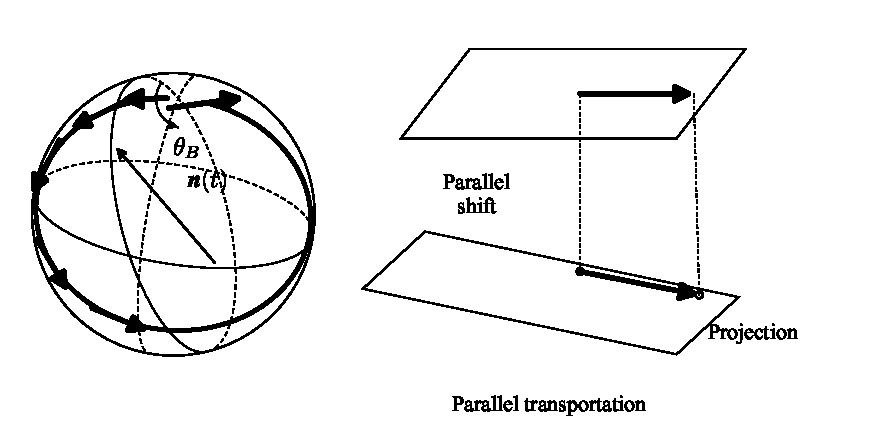
\includegraphics[width=0.72\textwidth]{fig_2.4.pdf}
\caption*{图 2.4\quad 自旋 1 相干态 $|\pmb{n}(t)\rangle$ 的相位的平行移动的几何表示。$|\pmb{n}(t)\rangle$ 的相位可以用单位球面上 $\pmb{n}(t)$ 点处切平面内的一个二维单位矢量来表示。在这种表示下，平行移动可以分解为两个几何操作：把二维矢量在三维空间中平移，再投影回倾斜的切平面。让一个二维切矢量绕闭合回路平行移动一周会使矢量转动，转角就是自旋 1 态的贝里相。（小回路的转角除以回路所围的面积即为球面的曲率。按照爱因斯坦的广义相对论，空间的曲率 $=$ 引力。）}
\end{figure}
贝里相也随之改变，即 $\theta_B \to \theta_B + \phi(0) - \phi(T)$。换言之，同一条路径 $\pmb{n}(t)$ 可以有不同的旋量表示 $z(t)$。不同的旋量表示给出不同的贝里相。

上面的讨论似乎表明，正如自旋态 $|\pmb{n}\rangle$ 的相位一样，贝里相也是非物理的。贝里相的起源似乎在于我们对不同自旋态相位的任意选取。于是，如果能为所有自旋态选出一个“共同”相位，就不会有贝里相。

让我们尝试沿路径 $\pmb{n}(t)$ 为自旋态 $|\pmb{n}(t)\rangle$ 选取一个共同相位，以便消去贝里相。我们先为路径起点的自旋态 $|\pmb{n}(0)\rangle$ 选定一个相位。然后在下一点为自旋态 $|\pmb{n}(\Delta t)\rangle$ 选取“相同相位”。这里的问题是：当 $\pmb{n}(0)$ 与 $\pmb{n}(\Delta t)$ 不同时，“相同相位”是什么意思？由于 $\pmb{n}(0)$ 与 $\pmb{n}(\Delta t)$ 近乎平行，$|\pmb{n}(0)\rangle$ 与 $|\pmb{n}(\Delta t)\rangle$ 几乎是同一个态。这意味着 $\bigl|\langle\pmb{n}(0)|\pmb{n}(\Delta t)\rangle\bigr| \approx 1$。于是我们可以定义：若 $\langle\pmb{n}(0)|\pmb{n}(\Delta t)\rangle$ 为实且正，则 $|\pmb{n}(0)\rangle$ 与 $|\pmb{n}(\Delta t)\rangle$ 具有相同相位。如果沿路径 $\pmb{n}(t)$ 对所有的态都这样选取相位，我们就定义了沿路径的一种“平行移动”（parallel transportation）（见图 2.4）。对这样的路径，我们有 $\langle\pmb{n}(0)|\frac{\mathrm{d}}{\mathrm{d}t}|\pmb{n}(t)\rangle = 0$。如果我们为路径上所有的自旋态选取了共同相位，贝里相就消失。

% ==================================================================
% 新增术语（ch2_c 新增，供术语表追加）：
%   spectral representation / spectral expansion 谱表示 / 谱展开；
%   analytic continuation 解析延拓；susceptibility（电介质与一般线性响应情形） 响应率；
%   conductance 电导；d.c. conductance 直流电导；Boltzmann factor 玻尔兹曼因子；
%   bosonic / fermionic (correlation) 玻色型 / 费米型（关联）；
%   (anti-)periodic （反）周期的；
%   contour 围道；spherical angles 球面角；solid angle 立体角；
%   spinor representation 旋量表示；parallel transportation 平行移动；
%   frustration 阻挫；geometric phase 几何相；tangent plane 切平面；
%   curvature 曲率；identity operator 恒等算符；direct product 直积；
%   equation of motion 运动方程；phase-space path integral 相空间路径积分
% ==================================================================

然而，对于闭合路径，我们也许无法为路径上所有的态挑选出一个共同的相位。这是因为，对于闭合路径，$|\pmb{n}(T)\rangle$ 与 $|\pmb{n}(0)\rangle$ 表示同一个自旋态，而由平行输运所确定的二者的相位选择可能并不一致。这一偏差恰好就是闭合路径的贝里相。选取自旋态的不同相位，即 $|\pmb{n}(t)\rangle \to \mathrm{e}^{\mathrm{i}\phi(t)}|\pmb{n}(t)\rangle$，会引起贝里相的改变 $\theta_B \to \theta_B + \phi(0) - \phi(T)$；由此我们看到，对于 $\pmb{n}(0) = \pmb{n}(T)$ 的闭合路径，贝里相是良定义的（在相差 $2\pi$ 的整数倍的意义下），因为 $\mathrm{e}^{\mathrm{i}\phi(0)} = \mathrm{e}^{\mathrm{i}\phi(T)}$。因此，讨论闭合路径的贝里相，或者比较具有相同起点与终点的两条路径的贝里相之差，都是有意义的。

我们看到，如果能为所有的态定义一个共同的相位，贝里相就为零。环路具有非零的贝里相，意味着不可能为环上所有的态选出一个共同的相位。贝里相的数值表示定义这种共同相位时的阻挫（frustration）程度。平行输运以及平行输运中的阻挫这些概念非常重要。电磁场与引力场都是广义的贝里相，它们描述的是某些更一般的矢量（而不是如上面所讨论的二维矢量，即复数）在平行输运中的阻挫。

贝里相是一种几何相位：只要两条路径 $\pmb{n}_1(t)$ 与 $\pmb{n}_2(t)$ 在单位球上描出相同的轨迹，它们就具有相同的贝里相。如果单位球上的轨迹 $\pmb{n}(t)$ 张出的立体角为 $\Omega$，那么该路径的贝里相就由下式给出（见问题 2.3.4）：
\begin{equation*}
\theta_B = \frac{\Omega}{2}\tag{2.3.5}
\end{equation*}

\subsection{贝里相与运动方程}

\begin{keypoints}
\item 贝里相可以影响系统的动力学性质。它可以改变运动方程。
\end{keypoints}

路径积分表示 (2.3.3) 可以推广到自旋-$S$ 系统，也可以推广到非零哈密顿量 $H = \pmb{B}\cdot\pmb{S}$ 的情形。相干态（即 $\pmb{n}\cdot\pmb{S}$ 的本征值最大（为 $S$）的本征态），记作 $|\pmb{n}\rangle$，可以写成上面讨论过的 $2S$ 个自旋-$\frac{1}{2}$ 相干态的直积：
\begin{equation*}
|\pmb{n}\rangle = |z\rangle \otimes |z\rangle \otimes \dots \otimes |z\rangle
\end{equation*}
于是，贝里相是自旋-$\frac{1}{2}$ 贝里相的 $2S$ 倍：
\begin{equation*}
\theta_B = \oint dt\, 2S\,\mathrm{i}\, z^{\dagger}\dot{z} = S\Omega\tag{2.3.6}
\end{equation*}
路径积分表示于是成为
\begin{equation*}
\mathrm{i}G(\pmb{n}_2, \pmb{n}_1, t) = \langle \pmb{n}_2 | U(t,0) | \pmb{n}_1 \rangle = \int \mathcal{D}\Big[\frac{\pmb{n}(t)}{2\pi}\Big]\, \mathrm{e}^{\mathrm{i}\int \mathrm{d}t\, [2S\,\mathrm{i}z^{\dagger}\dot{z} - \pmb{B}\cdot\pmb{n}S]}\tag{2.3.7}
\end{equation*}
让我们把
\begin{equation*}
S[\pmb{n}(t)] = \int \mathrm{d}t\, [2S\,\mathrm{i}z^{\dagger}\dot{z} - \pmb{B}\cdot\pmb{n}S]\tag{2.3.8}
\end{equation*}
当作一个经典作用量，并考虑由这样一个作用量所支配的自旋的经典运动。为得到经典运动方程，让我们比较 $S[\pmb{n}(t)]$ 与 $S[\pmb{n}(t)+\delta\pmb{n}(t)]$。（注意，路径 $\pmb{n}(t)$ 与 $\pmb{n}(t)+\delta\pmb{n}(t)$ 具有相同的起点和终点。）由贝里相 (2.3.6) 的几何解释可以发现，两条路径的贝里相之差等于 $S$ 乘以两条轨迹之间的面积：$\delta\theta_B = \int dt\, [S\pmb{n}\cdot(\dot{\pmb{n}}\times\delta\pmb{n})]$。于是，
\begin{equation*}
S[\pmb{n}(t)+\delta\pmb{n}(t)] - S[\pmb{n}(t)] = \int \mathrm{d}t\, [S\pmb{n}\cdot(\dot{\pmb{n}}\times\delta\pmb{n}) - \pmb{B}\cdot\delta\pmb{n}\,S]
\end{equation*}
这给出运动方程
\begin{equation*}
\pmb{n}\times\dot{\pmb{n}} = \pmb{B} - \pmb{n}(\pmb{n}\cdot\pmb{B})
\end{equation*}
（注意 $\delta\pmb{n}$ 总是垂直于 $\pmb{n}$），或者
\begin{equation*}
\dot{\pmb{S}} = \pmb{B}\times\pmb{S}\tag{2.3.9}
\end{equation*}
其中 $\pmb{S} = S\pmb{n}$ 对应于经典自旋矢量。这是一个奇怪的运动方程：速度（而不是加速度）正比于 $\pmb{B}$ 所代表的力。更奇怪的是，速度指向与力垂直的方向。然而，这恰好就是自旋的正确运动方程。我们看到，要恢复正确的自旋运动方程，贝里相是必不可少的。

\subsection*{问题 2.3.1}
证明图 2.4 中定义的 $\theta_B$ 实际上就是自旋-1 自旋的贝里相。

\subsection*{问题 2.3.2}
实际上，用不连续的路径 $s_z(t)$ 来描述自旋-$\frac{1}{2}$ 系统的路径积分表述也是可能的。设自旋-$\frac{1}{2}$ 系统的 $H = a\pmb{\sigma}^1 + b\pmb{\sigma}^3$，求时间演化算符 $\langle s_z'|U(t,0)|s_z\rangle$ 的路径积分表示。（提示：$\sum_{s_z=\pm 1/2}|s_z\rangle\langle s_z| = 1$。）

\subsection*{问题 2.3.3}
用旋量表示 (2.3.1) 计算闭合路径（$\phi = 0 \to 2\pi$，$\theta$ 固定）的贝里相。

对同一路径改用另一种旋量表示，计算贝里相：
\begin{equation*}
z = \begin{pmatrix} \cos\frac{\theta}{2} \\[2pt] \mathrm{e}^{-\mathrm{i}\phi}\sin\frac{\theta}{2} \end{pmatrix}
\end{equation*}
从这个例子我们看到，贝里相具有 $2\pi$ 的模糊性，依赖于所选的旋量表示。因此，贝里相 $\theta_B$ 不能直接用路径 $\pmb{n}$ 表示出来。这正是我们必须引入旋量表示来表述贝里相的原因。然而，$\mathrm{e}^{\mathrm{i}\theta_B}$ 是良定义的，并且只依赖于路径 $\pmb{n}(t)$。要得到一个良定义的路径积分，这已经足够。

\subsection*{问题 2.3.4}
对小闭合路径 $(\theta,\phi) \to (\theta+d\theta, \phi) \to (\theta+d\theta, \phi+d\phi) \to (\theta, \phi+d\phi) \to (\theta, \phi)$ 证明式 (2.3.5)。

对一般的大闭合路径证明式 (2.3.5)。

\subsection*{问题 2.3.5}
自旋与球面上的粒子：
\begin{enumerate}
\item 证明：设 $\pmb{B} = 0$，自旋作用量 (2.3.8) 可以写成
\begin{equation*}
S[\pmb{n}(t)] = \int \mathrm{d}t\, (A_{\theta}\dot{\theta} + A_{\phi}\dot{\phi})
\end{equation*}
求 $A_{\theta}$ 与 $A_{\phi}$。
\item 上述作用量可以看作下面这个作用量在 $m \to 0$ 极限下的结果：
\begin{equation*}
S_p[\pmb{n}(t)] = \int \mathrm{d}t\, \Big(A_{\theta}\dot{\theta} + A_{\phi}\dot{\phi} + \frac{1}{2}m\dot{\pmb{n}}^2\Big)
\end{equation*}
$S_p$ 描述一个质量为 $m$ 的粒子在单位球面上的运动。该粒子还经受一个由 $(A_{\phi}, A_{\theta})$ 所描述的磁场。证明 $(A_{\phi}, A_{\theta})$ 给出一个均匀磁场，并证明球面上的总磁通量子数为 $2S$。
\item 我们知道，均匀磁场中的粒子具有朗道能级结构。同一朗道能级中的所有态都具有相同的能量。各朗道能级被恒定的能隙 $\hbar\omega_c$ 分开，并且当 $m \to 0$ 时 $\omega_c \to \infty$。因此，在 $m \to 0$ 的极限下，只有第一朗道能级中的态出现在低能希尔伯特空间中。若均匀磁场的总磁通量子数为 $N_{\phi}$，求球面上粒子第一朗道能级中的态数。
\end{enumerate}

\subsection*{问题 2.3.6}
自旋波：考虑自旋-$S$ 量子自旋链 $H = \sum_i J\pmb{S}_i\cdot\pmb{S}_{i+1}$。当 $J < 0$ 时，经典基态是 $\pmb{S}_i = S\hat{z}$ 的铁磁态；当 $J > 0$ 时，是 $\pmb{S}_i = S\hat{z}(-)^i$ 的反铁磁态。
\begin{enumerate}
\item 写出自旋链的作用量。
\item 求围绕铁磁基态的小涨落 $\delta\pmb{S}_i = \pmb{S}_i - S\hat{z}$ 的运动方程。把运动方程变换到频率空间和动量空间，求出色散关系。证明对小的 $k$ 有 $\omega \propto k^2$。
\end{enumerate}

\begin{figure}[H]
\centering
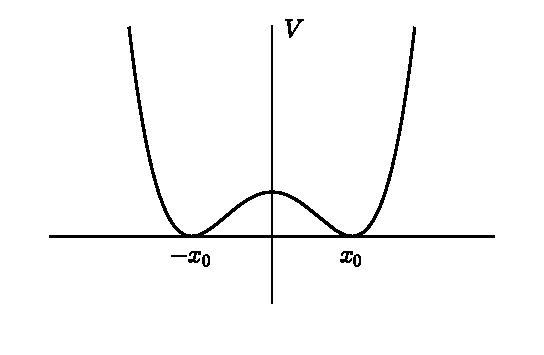
\includegraphics[width=0.72\textwidth]{fig_2.5.pdf}
\caption*{图 2.5\quad 双势阱。}
\end{figure}
\begin{figure}[H]
\centering
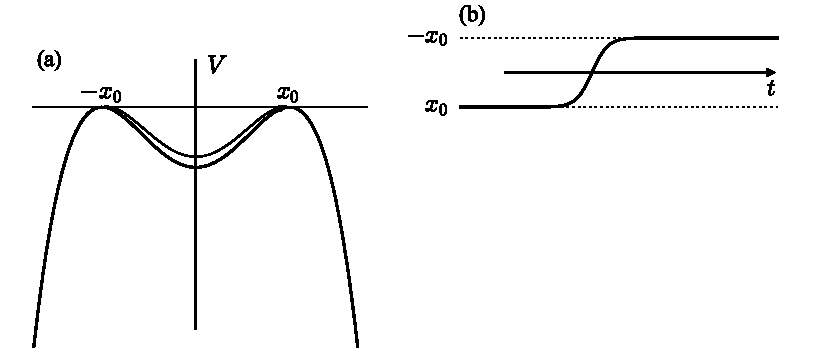
\includegraphics[width=0.72\textwidth]{fig_2.6.pdf}
\caption*{图 2.6\quad (a) 单个瞬子解可以视为倒转势的两个极大点之间的一种运动。(b) 同一运动在时空中的作图。}
\end{figure}
\begin{enumerate}
\setcounter{enumi}{2}
\item 求围绕反铁磁基态的小涨落 $\delta\pmb{S}_i = \pmb{S}_i - S\hat{z}(-)^i$ 的运动方程。求出色散关系。证明当 $k$ 接近 $\pi$ 时 $\omega \propto |k - \pi|$。
\end{enumerate}

有趣的是，铁磁态之上与反铁磁态之上的自旋波具有非常不同的色散。在经典统计物理中，铁磁态与反铁磁态具有相同的热力学性质；而正是贝里相使二者在量子层次上大不相同。

\section{路径积分表述的应用}

\subsection{穿越势垒的隧穿}

\begin{keypoints}
\item 有时，初始组态与最终组态由几条驻定路径相连。作用量最小的路径代表默认路径，其余路径代表瞬子效应。
\item 穿越势垒的隧穿是一种瞬子效应。
\end{keypoints}

\begin{figure}[H]
\centering
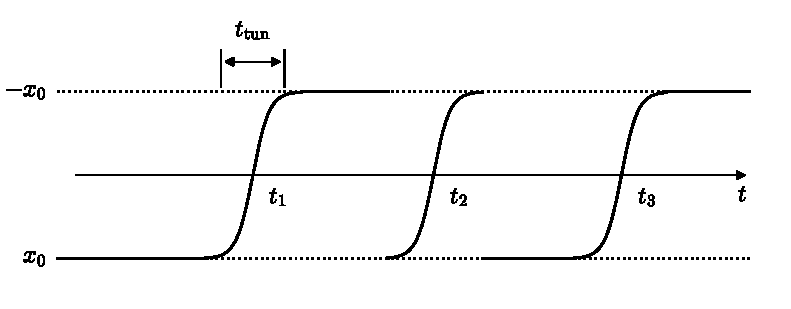
\includegraphics[width=0.72\textwidth]{fig_2.7.pdf}
\caption*{图 2.7\quad 多瞬子组态——瞬子气体。}
\end{figure}

路径积分不仅使我们能够计算诸如线性响应之类的微扰效应，还能使我们计算非微扰效应。这里我们想研究一个简单的例子，以理解路径积分如何给出非微扰的结果。我们将研究双势阱（图 2.5）中的隧穿。在没有隧穿时，粒子在某一极小点附近涨落，可用频率为 $\omega_0$ 的谐振子来描述。这些涨落给出如下传播子：
\begin{equation*}
\langle x_0|\mathrm{e}^{-TH}|x_0\rangle = \langle -x_0|\mathrm{e}^{-TH}|-x_0\rangle = \mathrm{e}^{-T\omega_0/2}, \quad \langle x_0|\mathrm{e}^{-TH}|-x_0\rangle = 0.
\end{equation*}
然而，由于隧穿，上述结果并不完全正确。有隧穿时，粒子可以在两个极小点之间来回穿行，传播子会获得一些额外的贡献。我们指出，隧穿是一种非微扰效应：围绕某一个极小点做微扰永远不可能给出隧穿。

为了研究隧穿效应，我们采用虚时路径积分和鞍点近似。除了分别连接 $x_0$ 到 $x_0$ 与 $-x_0$ 到 $-x_0$ 的两条平庸驻定路径 $x(t) = x_0$ 和 $x(t) = -x_0$ 之外，还有另一条连接 $x_0$ 与 $-x_0$ 的驻定路径。这样的路径使作用量 $\int \mathrm{d}\tau\,[\frac{1}{2}m\dot{x}^2 + V(x)]$ 取极小，并满足 $m\frac{\mathrm{d}^2 x}{\mathrm{d}\tau^2} = V'(x)$（译注：原文这两个公式分别印作含 $V'(x)$ 的作用量与 $m\frac{\mathrm{d}^2 x}{\mathrm{d}\tau^2} = V(x)$，撇号位置互易）。这是倒转势 $-V(x)$ 的牛顿方程（图 2.6(a)），其解如图 2.6(b) 所示。我们看到，在 $\pm x_0$ 之间的切换发生在一段很短的时间间隔内，这一事件称为一个瞬子（instanton）。图 2.6(b) 中的路径并不是连接 $x_0$ 与 $-x_0$ 的唯一驻定路径，图 2.7 中的多瞬子路径也是一条驻定路径。类似地，多瞬子路径还给出连接 $x_0$ 到 $x_0$ 以及 $-x_0$ 到 $-x_0$ 的其他驻定路径。

于是，为了计算传播子，我们需要对来自不同驻定路径的所有贡献求和。对于从 $x_0$ 到 $x_0$ 的传播子，我们有
\begin{align*}
\langle x_0|\mathrm{e}^{-TH}|x_0\rangle &= \mathrm{e}^{-T\omega_0/2} \sum_{n=\mathrm{even}} \int_0^T \mathrm{d}\tau_n \dots \int_0^{\tau_2} \mathrm{d}\tau_1 \left(K\mathrm{e}^{-S_0}\right)^n \\
&= \mathrm{e}^{-T\omega_0/2} \sum_{n=\mathrm{even}} \frac{T^n}{n!} \left(K\mathrm{e}^{-S_0}\right)^n = \cosh(TK\mathrm{e}^{-S_0})
\end{align*}
其中 $S_0$ 是瞬子的最小作用量，$K$ 来自围绕单个瞬子的涨落的路径积分。$K$ 应当具有频率的量纲，其数值大致由粒子撞击势垒的频率给出。类似地，我们还有
\begin{align*}
\langle x_0|\mathrm{e}^{-TH}|-x_0\rangle &= \mathrm{e}^{-T\omega_0/2} \sum_{n=\mathrm{odd}} \int_0^T \mathrm{d}\tau_n \dots \int_0^{\tau_2} \mathrm{d}\tau_1 \left(K\mathrm{e}^{-S_0}\right)^n \\
&= \mathrm{e}^{-T\omega_0/2} \sum_{n=\mathrm{odd}} \frac{T^n}{n!} \left(K\mathrm{e}^{-S_0}\right)^n = \sinh(TK\mathrm{e}^{-S_0})
\end{align*}
因此，
\begin{equation*}
\langle \psi_{\pm}|\mathrm{e}^{-TH}|\psi_{\pm}\rangle = \mathrm{e}^{-T\omega_0/2}\left[\cosh(TK\mathrm{e}^{-S_0}) \pm \sinh(TK\mathrm{e}^{-S_0})\right] = \mathrm{e}^{-T(\frac{\omega_0}{2} \pm K\mathrm{e}^{-S_0})}
\end{equation*}
其中 $|\psi_{\pm}\rangle = \frac{|x_0\rangle \pm |-x_0\rangle}{\sqrt{2}}$。我们看到 $|\psi_{\pm}\rangle$ 是能量本征态，其能量为 $E = \frac{\omega_0}{2} \pm K\mathrm{e}^{-S_0}$。

为了求出 $S_0$，注意到由能量守恒有 $\dot{x} = \sqrt{2V(x)/m}$。于是，
\begin{equation*}
S_0 = \int_{-\infty}^{+\infty} \mathrm{d}\tau\, \Big[\frac{1}{2}m\dot{x}^2 + V(x)\Big] = \int_{-x_0}^{+x_0} \mathrm{d}x\, \sqrt{2mV(x)}
\end{equation*}
恢复 $\hbar$ 后，我们得到 $\Delta E = 2K\mathrm{e}^{-\hbar^{-1}\int_{-x_0}^{+x_0} \mathrm{d}x\, \sqrt{2mV(x)}}$，这正是 WKB 结果。然而，路径积分确实教给我们一件新东西，即隧穿时间 $t_{tun}$——与单个瞬子相联系的时间尺度。对于粒子穿过一个势垒需要多长时间，我们有了一幅非常简单的图像。

\subsection*{问题 2.4.1}
设双势阱势由 $V(x) = \frac{g}{4}(x^2 - x_0^2)^2$ 给出。
\begin{enumerate}
\item 估算 $S_0$ 和隧穿时间 $t_{tun}$（即瞬子的大小）。
\item 设 $K \sim \sqrt{\frac{g x_0^2}{m}}$（这是极小点之一附近的振动频率），估算时间方向上瞬子的（平均）密度。
\end{enumerate}

\begin{figure}[H]
\centering
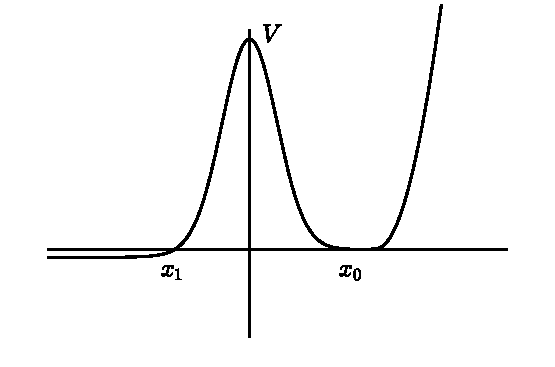
\includegraphics[width=0.72\textwidth]{fig_2.8.pdf}
\caption*{图 2.8\quad 具有亚稳态的势。}
\end{figure}
\begin{figure}[H]
\centering
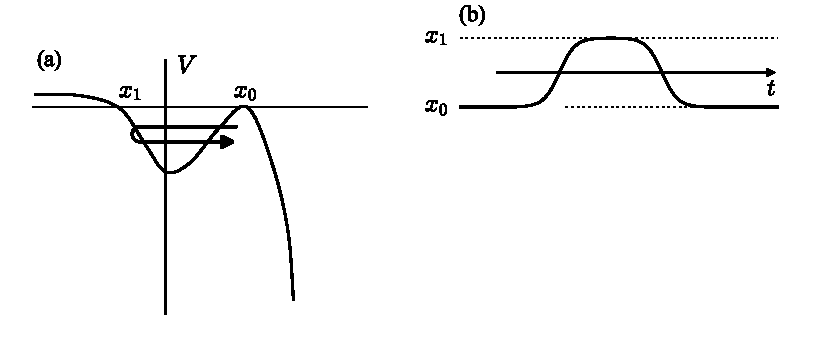
\includegraphics[width=0.72\textwidth]{fig_2.9.pdf}
\caption*{图 2.9\quad (a) 单次反弹解可以视为倒转势中的一种运动。(b) 同一运动在时空中的作图。}
\end{figure}
\begin{enumerate}
\setcounter{enumi}{2}
\item 若 $S_0 \gg 1$ 并且各瞬子互不重叠，半经典图像就是对隧穿的一种良好描述。问 $g$ 和 $x_0$ 取什么值时，上述两个条件都能满足？
\end{enumerate}

\subsection{亚稳态的命运}

\begin{keypoints}
\item 亚稳态的衰变也是一种瞬子效应。
\end{keypoints}

在本节中，我们考虑图 2.8 所示势 $V(x)$ 中的一个粒子。粒子初始时位于 $x_0$。我们想计算粒子穿过势垒逃逸的衰变率。为此我们计算 $\langle x_0|\mathrm{e}^{-TH}|x_0\rangle$。如果只考虑围绕 $x_0$ 的小涨落，则可以作近似 $V(x) = \frac{1}{2}m\omega_0^2(x - x_0)^2$，并对大的 $T$ 得到 $\langle x_0|\mathrm{e}^{-TH}|x_0\rangle = \mathrm{e}^{-T\omega_0/2}$。解析延拓到实时，我们看到 $\langle x_0|\mathrm{e}^{-\mathrm{i}TH}|x_0\rangle = \mathrm{e}^{-\mathrm{i}T\omega_0/2}$，没有衰变。为了找到衰变，我们需要寻找一个能使 $|\langle x_0|\mathrm{e}^{-\mathrm{i}TH}|x_0\rangle|$ 随时间减小的过程。我们将看到，隧穿可以引起衰变。在路径积分中，隧穿同样由瞬子来描述。

虚时拉格朗日量 $L = \frac{1}{2}m\dot{x}^2 + V(x)$ 有一条连接 $x_0$ 到 $x_0$ 的非平庸驻定路径 $x_c(t)$。这条驻定路径（称为一次反弹（bounce）或一个瞬子）的存在，可以从势 $-V(x)$ 中的经典运动看出来（图 2.9）。把反弹包括进来，并重复 2.4.1 节中的步骤，我们发现
\begin{align*}
\langle x_0|\mathrm{e}^{-TH}|x_0\rangle &= \mathrm{e}^{-T\omega_0/2} \sum_n \int_0^T \mathrm{d}\tau_n \int_0^{\tau_n} \mathrm{d}\tau_{n-1} \dots \int_0^{\tau_2} \mathrm{d}\tau_1 \left(K\mathrm{e}^{-S_0}\right)^n \\
&= \mathrm{e}^{-T(\frac{\omega_0}{2} - K\mathrm{e}^{-S_0})}\tag{2.4.1}
\end{align*}
其中 $S_0$ 是反弹的作用量，$K$ 是围绕反弹的涨落所产生的系数。乍看之下，反弹似乎只是把基态能量 $\frac{\omega_0}{2}$ 修正了一小量 $\Delta E = -K\mathrm{e}^{-S_0}$。由于反弹在经过很长时间后又回到 $x_0$，很难看出任何衰变。事实上我们将看到，系数 $K$ 是虚数，并且在实时 $\langle x_0|\mathrm{e}^{-\mathrm{i}TH}|x_0\rangle = \mathrm{e}^{-\mathrm{i}T\frac{\omega_0}{2} - T|K|\mathrm{e}^{-S_0}}$。反弹精确地描述了 $|x_0\rangle$ 态的衰变。这是一个相当惊人的结果。

为了理解 $K$ 为什么是虚数，我们需要讨论如何计算 $K$。这里的讨论同样适用于 2.4.1 节中隧穿振幅里的 $K$。

从我们在式 (2.4.1) 中纳入反弹的方式可以看到，$K\mathrm{e}^{-S_0}$ 是围绕 $x_c(t)$ 与围绕 $x = x_0$ 的两个路径积分之比：
\begin{equation*}
K\mathrm{e}^{-S_0} = \frac{\int_{x_c} \mathcal{D}\delta x\, \mathrm{e}^{-S}}{\int_{x=x_0} \mathcal{D}\delta x\, \mathrm{e}^{-S}}\tag{2.4.2}
\end{equation*}
对于小涨落，拉格朗日量可以展开到二阶。在 $x_c$ 附近，我们有
\begin{equation*}
S = S_0 + \int \mathrm{d}\tau\, \delta x \frac{1}{2}\Big[-m\frac{\mathrm{d}^2}{\mathrm{d}\tau^2} + V''(x_c(\tau))\Big]\delta x
\end{equation*}
而在 $x = x_0$ 附近有
\begin{equation*}
S = \int \mathrm{d}\tau\, \delta x \frac{1}{2}\Big[-m\frac{\mathrm{d}^2}{\mathrm{d}\tau^2} + V''(x_0)\Big]\delta x
\end{equation*}
于是，完成高斯积分后，我们得到
\begin{align*}
K &= \frac{\int_{x_c} \mathcal{D}\delta x\, \mathrm{e}^{-\int \mathrm{d}\tau\, \frac{1}{2}\delta x[-m\frac{\mathrm{d}^2}{\mathrm{d}\tau^2} + V''(x_c(\tau))]\delta x}}{\int_{x=x_0} \mathcal{D}\delta x\, \mathrm{e}^{-\int \mathrm{d}\tau\, \frac{1}{2}\delta x[-m\frac{\mathrm{d}^2}{\mathrm{d}\tau^2} + V''(x_0)]\delta x}} \\
&= \left(\frac{\operatorname{Det}\left(-m\frac{\mathrm{d}^2}{\mathrm{d}\tau^2} + V''(x_0)\right)}{\operatorname{Det}\left(-m\frac{\mathrm{d}^2}{\mathrm{d}\tau^2} + V''(x_c)\right)}\right)^{1/2}\tag{2.4.3}
\end{align*}
然而，式 (2.4.3) 是没有意义的，因为算符 $-m\frac{\mathrm{d}^2}{\mathrm{d}\tau^2} + V''(x_c)$ 具有一个零本征值。为了看清这一点，我们注意到 $x_c(\tau)$ 与 $x_c(\tau + \eta)$ 都是驻定路径，它们满足运动方程
\begin{equation*}
-m\frac{\mathrm{d}^2 x_c(\tau)}{\mathrm{d}\tau^2} + V'(x_c(\tau)) = -m\frac{\mathrm{d}^2 x_c(\tau+\eta)}{\mathrm{d}\tau^2} + V'(x_c(\tau+\eta)) = 0
\end{equation*}
将上式展开到 $\eta$ 的线性阶，我们发现 $\eta\dot{x}_c(\tau) = x_c(\tau+\eta) - x_c(\tau)$ 满足
\begin{equation*}
\Big[-m\frac{\mathrm{d}^2}{\mathrm{d}\tau^2} + V''(x_c(\tau))\Big]\dot{x}_c(\tau) = 0
\end{equation*}
于是，$\dot{x}_c(\tau)$ 是 $\left(-m\frac{\mathrm{d}^2}{\mathrm{d}\tau^2} + V''(x_c)\right)$ 的一个零本征值本征态。

从上面的讨论同样可以清楚地看到，零模 $\eta\dot{x}_c(\tau)$ 对应于反弹的位置，而反弹的位置在式 (2.4.1) 中已经被积分过了。因此，式 (2.4.2) 并不完全正确。实际上我们有
\begin{equation*}
\int \mathrm{d}\tau_1\, K\mathrm{e}^{-S_0} = \frac{\int_{x_c} \mathcal{D}\delta x\, \mathrm{e}^{-S}}{\int_{x=x_0} \mathcal{D}\delta x\, \mathrm{e}^{-S}}\tag{2.4.4}
\end{equation*}
为了计算式 (2.4.4)，我们需要更仔细地定义路径积分。设 $x_n(\tau)$ 是算符 $-m\frac{\mathrm{d}^2}{\mathrm{d}\tau^2} + V''(x_c)$ 的第 $n$ 个归一化本征态，则 $\delta x$ 可以写成 $\delta x = \sum c_n x_n(\tau)$，并且可以定义一个截断的“配分函数”：
\begin{align*}
Z_N(x_c) &\equiv A_N \int \prod_1^N \frac{\mathrm{d}c_n}{\sqrt{2\pi}}\, \mathrm{e}^{-\int \mathrm{d}\tau\, \frac{1}{2}\delta x(-m\frac{\mathrm{d}^2}{\mathrm{d}\tau^2} + V''(x_c(\tau))]\delta x} \\
&= A_N \left(\operatorname{Det}_N\left(-m\frac{\mathrm{d}^2}{\mathrm{d}\tau^2} + V''(x_c)\right)\right)^{-1/2}
\end{align*}
其中 $\operatorname{Det}_N$ 只包括前 $N$ 个本征值的乘积。真正的“配分函数” $Z$ 是 $Z_N$ 在 $N \to \infty$ 下的极限。由于零模 $x_1(\tau)$，上述结果需要修改。我们需要把零模分离出来，得到
\begin{equation*}
Z_N(x_c) = A_N \int \frac{\mathrm{d}c_1}{\sqrt{2\pi}} \left(\operatorname{Det}_N'\left(-m\frac{\mathrm{d}^2}{\mathrm{d}\tau^2} + V''(x_c)\right)\right)^{-1/2}
\end{equation*}
其中 $\operatorname{Det}'$ 表示不包含零本征值。

积分 $\int \mathrm{d}c_1$ 实际上是对反弹位置的积分，也就是 $\int \mathrm{d}\tau_1$。可以求出 $c_1$ 与 $\tau_1$ 通过 $\mathrm{d}\tau_1 = \frac{\mathrm{d}c_1}{\sqrt{S_0/m}}$ 相联系。\footnote{我们注意到
\begin{equation*}
\frac{m}{2}\frac{\mathrm{d}}{\mathrm{d}\tau}(\dot{x}_c)^2 = m\dot{x}_c\ddot{x}_c = \dot{x}_c V'(x_c) = \frac{\mathrm{d}}{\mathrm{d}\tau}V(x_c)
\end{equation*}
因此，若假定 $V(x_0) = 0$，则有 $\frac{m}{2}(\dot{x}_c)^2 = V(x_c)$。由于
\begin{equation*}
S_0 = \int \mathrm{d}\tau\, \Big[\frac{1}{2}m\dot{x}_c^2 + V(x_c)\Big] = \int \mathrm{d}\tau\, m\dot{x}_c^2
\end{equation*}
归一化的零模具有如下形式：
\begin{equation*}
x_1(\tau) = \frac{\dot{x}_c(\tau)}{\sqrt{S_0/m}}
\end{equation*}
于是，$\delta x = c_1 x_1$ 将使反弹产生位移 $\delta\tau = \frac{c_1}{\sqrt{S_0/m}}$。这使我们能够把 $\mathrm{d}c_1$ 换成 $\mathrm{d}\tau_1$。}

因此，
\begin{equation*}
Z_N(x_c) = A_N \int \mathrm{d}\tau_1\, \sqrt{\frac{S_0}{2\pi m}} \left(\operatorname{Det}_N'\left(-m\frac{\mathrm{d}^2}{\mathrm{d}\tau^2} + V''(x_c)\right)\right)^{-1/2}\tag{2.4.5}
\end{equation*}
类似地，对于围绕 $x = x_0$ 的路径积分，我们也可以引入 $Z_N(x_0)$：
\begin{equation*}
Z_N(x_0) = A_N \left(\operatorname{Det}_N\left(-m\frac{\mathrm{d}^2}{\mathrm{d}\tau^2} + V''(x_0)\right)\right)^{-1/2}\tag{2.4.6}
\end{equation*}
现在我们可以写出
\begin{equation*}
\int \mathrm{d}\tau\, K = \lim_{N\to\infty} \frac{Z_N(x_c)}{Z_N(x_0)}
\end{equation*}
由此得到
\begin{align*}
K &= \sqrt{\frac{S_0}{2\pi m}} \left(\frac{\operatorname{Det}\left(-m\frac{\mathrm{d}^2}{\mathrm{d}\tau^2} + V''(x_0)\right)}{\operatorname{Det}'\left(-m\frac{\mathrm{d}^2}{\mathrm{d}\tau^2} + V''(x_c)\right)}\right)^{1/2} \\
&= \sqrt{\frac{S_0}{2\pi}} \left(\frac{\operatorname{Det}\left(-\frac{\mathrm{d}^2}{\mathrm{d}\tau^2} + m^{-1}V''(x_0)\right)}{\operatorname{Det}'\left(-\frac{\mathrm{d}^2}{\mathrm{d}\tau^2} + m^{-1}V''(x_c)\right)}\right)^{1/2}\tag{2.4.7}
\end{align*}
其中用到了这样一个事实：$\operatorname{Det}$ 比 $\operatorname{Det}'$ 多包含一个本征值。同一事实还告诉我们，$K$ 具有 $\tau^{-1}$ 的量纲。

$-\frac{\mathrm{d}^2}{\mathrm{d}\tau^2} + m^{-1}V''(x_0)$ 的所有本征值都是正的。算符 $-\frac{\mathrm{d}^2}{\mathrm{d}\tau^2} + m^{-1}V''(x_c)$ 包含一个零模 $\dot{x}_c(\tau)$，它有一个节点。因此，$-\frac{\mathrm{d}^2}{\mathrm{d}\tau^2} + m^{-1}V''(x_c)$ 有一个、并且只有一个负本征值，正是它使 $K$ 成为虚数。

同一公式 (2.4.7) 也适用于 2.4.1 节中所考虑的隧穿问题。不过，在该情形中零模 $\dot{x}_c$ 没有节点，$-\frac{\mathrm{d}^2}{\mathrm{d}\tau^2} + m^{-1}V''(x_c)$ 没有负本征值。因此，对隧穿问题来说 $K$ 是实数。

我们已经提到，系数 $K$ 来自围绕驻定路径的涨落。从上面的计算我们看到，如果只计入小涨落，$K$ 就可以用算符行列式来表示。Coleman (1985) 讨论过计算行列式之比的若干方法，我在此不再深入。

可能有人已经意识到，眼前这个问题用 WKB 方法很容易解决。路径积分方法实在太繁琐了，人们也许会问，为什么我们还要费心讨论它。进行这一讨论的动机，首先在于它展示了一次典型的路径积分计算中的各个步骤及其微妙之处；其次，也是更重要的一点，同一方法可以用来研究场论中亚稳态的衰变。

\subsection*{问题 2.4.2}
带有衰变亚稳态的最简单场论模型由下式给出：
\begin{equation*}
S = \int \mathrm{d}t\, \mathrm{d}^d\pmb{x}\, \left[\frac{1}{2}\left[(\partial_t m)^2 - v^2(\partial_{\pmb{x}} m)^2\right] - \frac{g}{4}(m^2 - m_0^2)^2 - Bm\right]
\end{equation*}
其中 $m(t, \pmb{x})$ 是一个实场，可以把它看作磁矩的密度。我们将选取单位使速度 $v = 1$。当磁场 $B$ 为零时，系统有两个简并的基态 $m = \pm m_0$，它们是势 $V(m) = \frac{g}{4}(m^2 - m_0^2)^2 + Bm$ 的两个极小点。
\begin{enumerate}
\item 证明：当 $B$ 较小时，系统有一个基态 $m = m_+$ 和一个亚稳态 $m = m_-$。但当 $B$ 超过临界值 $B_c$ 时，亚稳态便不复存在。求 $B_c$ 的值。
\item 写出虚时中的作用量。Coleman 证明，该作用量总有如下形式的反弹解（一条驻定路径）：
\begin{equation*}
m = f\left(\sqrt{(\tau - \tau_0)^2 + (\pmb{x} - \pmb{x}_0)^2}\right) + m_-, \qquad f(\infty) = 0
\end{equation*}
其中 $(\tau_0, \pmb{x}_0)$ 是反弹的位置。
\item 假定在没有反弹时 $\langle m_-|\mathrm{e}^{-TH}|m_-\rangle = \mathrm{e}^{-TE_0}$。把反弹包括进来之后，我们有
\begin{equation*}
\langle m_-|\mathrm{e}^{-TH}|m_-\rangle = \mathrm{e}^{-TE_0} \sum_n \frac{1}{n!} \int \prod_{i=1}^n \mathrm{d}\tau_i\, \mathrm{d}^d\pmb{x}_i\, K^n \mathrm{e}^{-nS_0}
\end{equation*}
其中 $S_0$ 是反弹的作用量，$(\tau_i, \pmb{x}_i)$ 是各个反弹的位置。（注意，现在一个反弹由它在时间与空间两个方面的位置来参数化。）若 $K$ 是虚数，亚稳态 $|m_-\rangle$ 的衰变率是多少？单位体积的衰变率是多少？
\item 设 $B = \frac{B_c}{2}$，估算 $S_0$ 的值。（提示：对 $(\tau, \pmb{x})$ 和 $m$ 重新标度，把 $S$ 改写为 $S = \text{constant} \times S'$，使 $S'$ 中所有系数都是 1 的量级。）（用这一方法也可以估计反弹在时空中的大小。）
\item 设 $B = \frac{B_c}{2}$，估算 $K$ 的值。（提示：考虑当 $S \to aS$ 时 $K$ 如何标度。）
\end{enumerate}

% ------------------------------------------------------------
% 块边界备注：
%   起点：书页 46（ch2_c）末段完整结束（"...The Berry phase vanishes if we
%   choose a common phase for all of the spin states on the path."），
%   书页 47 顶部为空格缩进的新段落（However, for a closed path...），
%   故本块正文直接以该新段开始，无需 %JOIN%，也无 ch2_c 收尾内容可写入
%   %--C-TAIL-- 区（按 assemble.py 约定该区只放"上一文件收尾"）。
%   终点：书页 57 末为止于问题 2.4.2 第 5 问；书页 58 顶部为第 6 问
%   （Discuss for which values of g and m_0 ...），按装配约定归 ch2_e
%   的 %--D-TAIL--，本块未收，ch2_e 请勿重复翻译本块已有的第 1–5 问。
% ------------------------------------------------------------
% 新增术语（ch2_d，待并入术语表"新增术语"区）：
%   instanton 瞬子
%   multi-instanton 多瞬子
%   instanton gas 瞬子气体
%   bounce 反弹
%   tunneling 隧穿
%   tunneling time 隧穿时间
%   barrier 势垒
%   double-well potential 双势阱
%   meta-stable state 亚稳态
%   decay rate 衰变率
%   frustration 阻挫
%   parallel transportation 平行输运
%   geometric phase 几何相位
%   solid angle 立体角
%   direct product 直积
%   spin chain 自旋链
%   spin wave 自旋波
%   ferromagnetic state 铁磁态
%   anti-ferromagnetic state 反铁磁态
%   dispersion relation 色散关系
%   non-perturbative effect 非微扰效应
%   zero mode 零模
%   zero eigenvalue 零本征值
%   node 节点
%   determinant 行列式
%   Hilbert space 希尔伯特空间
%   Newton's equation 牛顿方程
%   magnetic moment 磁矩
%   flux quanta 磁通量子
%   Landau level structure 朗道能级结构
% ------------------------------------------------------------

% 本块顶部为问题 2.4.2 的第 6 问（题干与小问 1–5 在 ch2_d 末尾），装配器会接回第 5 问之后。
\begin{enumerate}
\item[6.] 讨论对 $g$ 与 $m_0$ 的哪些取值，半经典隧穿（tunneling）图像才是对亚稳态（meta-stable state）衰变的一个好的描述。
\end{enumerate}
%--D-TAIL 结束--

\subsection{摩擦的量子理论}

\begin{keypoints}
\item 量子系统中的耗散（摩擦）可以通过让系统与一个热库（heat bath，即一组谐振子）耦合来模拟。
\end{keypoints}

粒子受到的摩擦来自它与环境的耦合。由于这种耦合，粒子会把能量丢失到环境中。因此，要建立摩擦的量子理论，我们必须把与环境的耦合包含进来。这里我们用一组谐振子来模拟环境（Caldeira and Leggett, 1981）。我们需要搭建一个能给出有限摩擦系数（friction coefficient）的恰当环境。这使我们能够理解存在摩擦时粒子的量子运动。

我们的模型由如下路径积分描述：
\begin{equation*}
Z = \text{常数} \times \int \mathcal{D}[x(t)]\,\mathcal{D}[h_i(t)]\;\mathrm{e}^{\mathrm{i}\int \mathrm{d}t\,\left(\frac{1}{2}m\dot{x}^2 + \sum_i \frac{1}{2}\dot{h}_i^2 - \frac{1}{2}(\Omega_i h_i + g_i x)^2\right)}
\end{equation*}
（译注：原书此式指数中第一项误排为 $\frac{1}{2}m\dot{x}$，遗漏了平方；现按式 (2.4.8) 改正为 $\frac{1}{2}m\dot{x}^2$。）

其中 $x$ 是粒子的坐标，诸 $h_i$ 描述一簇谐振子。注意我们的系统具有平移对称性 $x \to x + \text{常数}$。把 $h_i$ 积掉之后，我们得到（见 2.2.3 节）
\begin{equation*}
Z = \text{常数} \times \int \mathcal{D}[x(t)]\;\mathrm{e}^{\mathrm{i}\int \mathrm{d}t\,\frac{m}{2}\dot{x}^2 + \mathrm{i}\int \mathrm{d}t\,\mathrm{d}t'\,\frac{1}{4}G_{\mathrm{os}}(t-t')(x(t)-x(t'))^2} \tag{2.4.8}
\end{equation*}
其中
\begin{align*}
G_{\mathrm{os}}(t-t') &= \sum_i \Omega_i^2 g_i^2 (-\mathrm{i})\langle h_i(t)h_i(0)\rangle = -\mathrm{i}\sum_i \frac{g_i^2\Omega_i}{2}\,\mathrm{e}^{-\mathrm{i}|t-t'|\Omega_i}\\
&= -\mathrm{i}\int_0^{\infty} \mathrm{d}\Omega\; n(\Omega)\,\frac{\Omega g^2(\Omega)}{2}\,\mathrm{e}^{-\mathrm{i}|t-t'|\Omega},
\end{align*}
$n(\Omega) \equiv \sum_i \delta(\Omega - \Omega_i)$ 是态密度（density of states），而 $g^2(\Omega) \equiv \sum_i g_i^2\delta(\Omega - \Omega_i)/\sum_i \delta(\Omega - \Omega_i)$。式 (2.4.8) 中的双时作用量（double-time action）给出如下运动方程：
\begin{equation*}
-\omega^2 m x_\omega = -(G_{\mathrm{os}}(\omega) - G_{\mathrm{os}}(0))\, x_\omega,
\end{equation*}
它可以改写为\footnote{这里我们用了 $\mathrm{Im}G_{\mathrm{os}}(\omega = 0) = 0$。注意 $\mathrm{Im}D_{\mathrm{os}}(\omega) = -\mathrm{Im}D_{\mathrm{os}}(-\omega)$，因而 $\mathrm{Im}D_{\mathrm{os}}(\omega = 0) = 0$。由于 $\mathrm{Im}G_{\mathrm{os}}(\omega) = \mathrm{sgn}(\omega)\mathrm{Im}D_{\mathrm{os}}(\omega)$，我们发现 $\mathrm{Im}G_{\mathrm{os}}(\omega = 0) = 0$。}
\begin{align*}
-\omega^2 m^* x_\omega &= -(-\mathrm{i}\omega)\gamma x_\omega, \tag{2.4.9}\\
m^* &= m - \frac{\mathrm{Re}(G_{\mathrm{os}}(\omega) - G_{\mathrm{os}}(0))}{\omega^2}, \qquad \gamma = -\frac{\mathrm{Im}G_{\mathrm{os}}(\omega)}{\omega}
\end{align*}
若 $m^*$ 与 $\gamma$ 在小 $\omega$ 下有限，则式 (2.4.9) 变为 $m^*\frac{\mathrm{d}^2x}{\mathrm{d}t^2} = -\gamma\frac{\mathrm{d}x}{\mathrm{d}t}$，它描写一个质量为 $m^*$ 的粒子，其摩擦由摩擦系数 $\gamma$ 描述。我们看到，与一簇谐振子的耦合可以在粒子上产生摩擦。摩擦（因而是耗散）来自关联的虚部 $\mathrm{Im}G_{\mathrm{os}}(\omega)$。这种耦合还把粒子的质量从 $m$ 改变为 $m^*$。这里 $m^*$ 称为粒子的有效质量（effective mass）。修正量 $m^* - m$ 来自关联的实部 $\mathrm{Re}G_{\mathrm{os}}(\omega)$。物理上，粒子使谐振子发生形变，形变随粒子一起运动，从而改变了粒子的有效质量。

上面的摩擦量子理论有一个问题。由于 $\mathrm{Im}G_{\mathrm{os}}(\omega) < 0$，我们看到摩擦系数 $\gamma(\omega) > 0$（当 $\omega > 0$），这是正确的；然而当 $\omega < 0$ 时 $\gamma(\omega) < 0$，这似乎毫无道理。我们注意到，式 (2.4.8) 中的有效作用量在时间反演（time reversal）$t \to -t$ 下不变。其后果是：如果 $\omega > 0$ 的解对应于衰减过程，那么 $\omega < 0$ 的解就对应于衰减过程的逆过程。

要真正地描述摩擦，我们需要一个不具有时间反演不变性的形式框架。为此，重要的是注意到：在存在摩擦时，$t = -\infty$ 处的态（即 $|0_-\rangle$）与 $t = \infty$ 处的态（即 $|0_+\rangle$）是非常不同的，因为随着粒子慢下来，谐振子被激发到越来越高的态。这使得我们的路径积分 $Z = \langle 0|U(\infty,-\infty)|0\rangle$ 成为一个糟糕的出发点，因为它等于零。于是，这里的问题是为非平衡系统构造路径积分。闭合时间路径积分（closed-time path integral），或称 Schwinger–Keldysh 形式（Schwinger, 1961; Keldysh, 1965; Rammer and Smith, 1986），是解决这些问题的一条途径。Schwinger–Keldysh 形式从一个不同的路径积分 $Z_{\mathrm{close}} = \langle 0|U(-\infty,\infty)U(\infty,-\infty)|0\rangle$ 出发，它从 $t = -\infty$ 走到 $t = +\infty$ 再返回 $t = -\infty$。

上面发展的双时路径积分（double-time path integral）(2.4.8) 只能描写耗散系统的平衡性质，例如存在摩擦/耗散时围绕基态的涨落。它不能描写非平衡性质，例如由摩擦引起的速度减慢，因为这涉及 $t = \pm\infty$ 处两个不同的态 $|0_-\rangle$ 与 $|0_+\rangle$。

这里遇到的问题与 2.2 节中遇到的问题类似，在那里我们曾试图用路径积分计算响应率的虚部——它同样与耗散相联系。在那里，问题是靠把编时关联函数换成响应函数而解决的。这里的问题可以用同样的方式解决（或者更确切地说，用手工方式加以修正）。如果在\emph{运动方程}中把 $G_{\mathrm{os}}(\omega)$ 换成 $D_{\mathrm{os}}(\omega)$（注意 $D_{\mathrm{os}}(t) = 2\Theta(t)\mathrm{Re}G_{\mathrm{os}}(t)$）——但在双时路径积分中不作这种替换——那么摩擦系数 $\gamma$ 将由
\begin{equation*}
\gamma = -\frac{\mathrm{Im}D_{\mathrm{os}}(\omega)}{\omega} \tag{2.4.10}
\end{equation*}
给出，它对 $\omega > 0$ 与 $\omega < 0$ 都总是正的。在记住上述限制的前提下，我们可以说双时路径积分 (2.4.8) 能够描述一个有摩擦的系统。摩擦系数由式 (2.4.10) 给出。

由于
\begin{equation*}
G_{\mathrm{os}}(\omega) = \int_0^{\infty} \mathrm{d}\Omega\;\frac{\Omega^2 n(\Omega)g^2(\Omega)}{\omega^2 - \Omega^2 + \mathrm{i}0^+},
\end{equation*}
我们求得 $\mathrm{Im}G_{\mathrm{os}}(\omega) = -\frac{\pi}{2}|\omega|n(|\omega|)g^2(|\omega|)$。利用 $\mathrm{Im}D_{\mathrm{os}}(\omega) = \mathrm{sgn}(\omega)\mathrm{Im}G_{\mathrm{os}}(\omega)$ 这一事实，我们求得对小 $\omega$ 值
\begin{equation*}
\gamma = \frac{\pi}{2}\, n(|\omega|)\, g^2(|\omega|) \tag{2.4.11}
\end{equation*}
因此，要使 $\gamma$ 在小 $\omega$ 下有限，我们要求当 $\Omega \to 0$ 时 $n(\Omega)g^2(\Omega)$ 有限。

让我们假设当 $\Omega < \Omega_0$ 时 $n(\Omega)g^2(\Omega) = n_0 g_0^2$，而当 $\Omega > \Omega_0$ 时 $n(\Omega)g^2(\Omega) = 0$。我们求得
\begin{align*}
G_{\mathrm{os}}(\omega) &= -n_0 g_0^2 \Omega_0 + \frac{n_0 g_0^2|\omega|}{2}\ln\left|\frac{\Omega_0 + |\omega|}{\Omega_0 - |\omega|}\right| - \mathrm{i}\,\frac{\pi}{2}|\omega|\, n_0 g_0^2\\
G_{\mathrm{os}}(t) &= \mathrm{i}\,\frac{n_0 g_0^2}{2t^2}\left(1 - (\mathrm{i}|t|\Omega_0 + 1)\,\mathrm{e}^{-\mathrm{i}|t|\Omega_0}\right)
\end{align*}
除了有限的摩擦系数 $\gamma = \frac{\pi}{2}n_0 g_0^2$ 之外，我们还得到有效质量 $m^* = m - \frac{n_0 g_0^2}{\Omega_0^2}$。

我们想指出，$G_{\mathrm{os}}(t)$ 中的 $(\mathrm{i}|t|\Omega_0 + 1)\mathrm{e}^{-\mathrm{i}|t|\Omega_0}$ 项来自 $n(\Omega)g^2(\Omega)$ 在 $\Omega = \Omega_0$ 处的不连续性。如果 $n(\Omega)g^2(\Omega)$ 是 $\Omega$ 的光滑函数，那么这一项在大 $t$ 极限下将指数式地消失。例如，若选取 $n(\Omega)g^2(\Omega) = n_0 g_0^2\,\mathrm{e}^{-\Omega^2/\Omega_0^2}$，则在大 $t$ 极限下将有 $G_{\mathrm{os}}(t) = \mathrm{i}\frac{n_0 g_0^2}{2t^2}$。摩擦系数仍由 $\gamma = \mathrm{sgn}(\omega)\frac{\pi}{2}n_0 g_0^2$ 给出。采用这样的 $n(\Omega)g^2(\Omega)$ 选择之后，我们发现一个具有摩擦 $\gamma = \frac{\pi}{2}n_0 g_0^2$ 的粒子由如下双时作用量描述：
\begin{equation*}
S = \int \mathrm{d}t\;\frac{m}{2}\dot{x}^2 + \mathrm{i}\int \mathrm{d}t\,\mathrm{d}t'\;\frac{\gamma\,(x(t) - x(t'))^2}{4\pi(t - t')^2} \tag{2.4.12}
\end{equation*}

\begin{figure}[H]
\centering
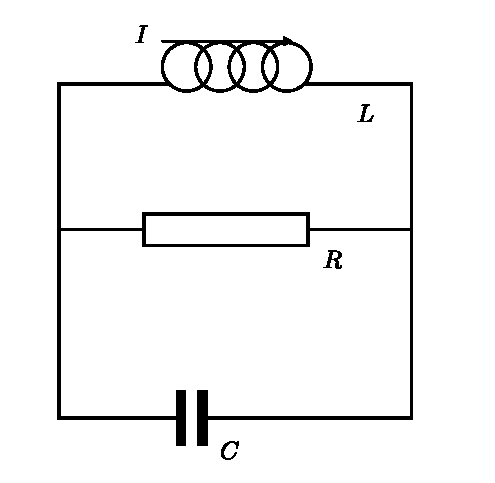
\includegraphics[width=0.72\textwidth]{fig_2.10.pdf}
\caption*{图 2.10\quad 一个 RCL 电路。}
\end{figure}

\subsection*{问题 2.4.3}

\textbf{有效质量：}
\begin{enumerate}
\item[1.] 假设对小 $\Omega$ 有 $n(\Omega)g^2(\Omega) \propto \Omega^\alpha$，且当 $\Omega > \Omega_0$ 时 $n(\Omega)g^2(\Omega) = 0$。求出使有效质量 $m^*$ 发散的 $\alpha$ 值。
\item[2.] 考虑 $n(\Omega)g^2(\Omega) = N_0\,\mathrm{e}^{-\Omega/\Omega_0}$ 与 $n(\Omega)g^2(\Omega) = N_0\,\mathrm{e}^{-(\Omega/\Omega_0)^2}$ 两种情形。哪一种情形的有效质量发散？
\end{enumerate}

\subsection{RCL 电路的量子理论}

\begin{keypoints}
\item RCL 电路的量子动力学与一个带摩擦粒子的量子动力学类似。
\item 如何在一个量子 RCL 电路中纳入电荷量子化（charge quantization）。
\end{keypoints}

RCL 电路是一个简单的电路，我们知道如何在经典层次上描述它。既然一切都被认为是用量子理论描述的，问题就产生了：如何用量子力学来描述一个 RCL 电路？

让我们先考虑电容为 $C$ 的一个理想电容器。电容器的态由其电荷 $q$ 描述；如果我们忽略电荷量子化，$q$ 是一个实数。理想电容器的量子理论很简单：希尔伯特空间由态 $\{|q\rangle\}$ 张成，哈密顿量为 $H = \frac{\hat{q}^2}{2C}$，其中电荷算符 $\hat{q}$ 定义为 $\hat{q}|q\rangle = q|q\rangle$。于是，一个量子电容器等价于一条直线上的自由粒子，$q$ 是它的“动量”。哈密顿量 $H = \frac{\hat{q}^2}{2C}$ 的形式告诉我们，这个粒子的质量恰为 $C$。相应的经典拉格朗日量为 $L = \frac{1}{2}C\dot{x}^2$。

为了描述一个 CL 电路，我们加入一个势能项，考虑
\begin{equation*}
L_{\mathrm{CL}} = \frac{C}{2}\dot{x}^2 - \frac{1}{2L}x^2 \tag{2.4.13}
\end{equation*}
由此得到的运动方程为
\begin{equation*}
C\frac{\mathrm{d}^2x}{\mathrm{d}t^2} = -\frac{x}{L}
\end{equation*}
如果我们把 $x/L$ 解释为电流 $I$、把 $L$ 解释为电感，它与 CL 电路的方程
\begin{equation*}
V = \frac{q}{C} = L\frac{\mathrm{d}I}{\mathrm{d}t}, \qquad\qquad I = -\frac{\mathrm{d}q}{\mathrm{d}t},
\end{equation*}
等价。我们看到，CL 电路等价于一个坐标为 $x$、质量为 $C$、弹簧常数为 $1/L$ 的谐振子。于是，量子 CL 电路由哈密顿量
\begin{equation*}
H = \frac{1}{2C}\hat{q}^2 + \frac{1}{2L}\hat{x}^2 \tag{2.4.14}
\end{equation*}
描述，其中 $\hat{q}$ 是电荷算符；它也是与 $\hat{x}$ 共轭的动量算符，满足 $[\hat{q}, \hat{x}] = \mathrm{i}$。流算符由 $\hat{I} \equiv \hat{x}/L$ 给出。

我们也可以把 $q$ 视为坐标，而把 $-x$ 视为相应的“动量”。在这种观点下，哈密顿量 (2.4.14) 给出如下拉格朗日量，它是式 (2.4.13) 的对偶形式（dual form）：
\begin{equation*}
L_{\mathrm{CL}}^d = \frac{L}{2}\dot{q}^2 - \frac{1}{2C}q^2 \tag{2.4.15}
\end{equation*}
如图 2.10 所示，在加入一个电阻器之后，经典运动方程变为
\begin{equation*}
V = \frac{q}{C} = L\frac{\mathrm{d}I}{\mathrm{d}t}, \qquad\qquad I = -\frac{\mathrm{d}q}{\mathrm{d}t} - V/R
\end{equation*}
由此得到
\begin{equation*}
C\frac{\mathrm{d}^2x}{\mathrm{d}t^2} = -\frac{x}{L} - \frac{1}{R}\frac{\mathrm{d}x}{\mathrm{d}t} \tag{2.4.16}
\end{equation*}
这正是摩擦系数为 $\gamma = 1/R$ 的粒子的运动方程。这样的系统可以用一个双时作用量描述（见式 (2.4.12)）：
\begin{equation*}
S_{\mathrm{RCL}} = \int \mathrm{d}t\,\left(\frac{1}{2}C\dot{x}^2 - \frac{1}{2L}x^2\right) + \mathrm{i}\int \mathrm{d}t\,\mathrm{d}t'\;\frac{(x(t) - x(t'))^2}{4\pi R(t - t')^2} \tag{2.4.17}
\end{equation*}
RCL 电路的许多量子动力学性质都可以由上述作用量计算出来。

如果我们计入电荷量子化，那么电荷为 $q = e^{*} \times \text{整数}$。由于电荷 $q$ 也是 $x$ 的动量，动量的量子化意味着粒子生活在一个圆上。电荷（即动量）量子 $e^{*}$ 意味着 $x$ 与 $x + \frac{2\pi}{e^{*}}$ 应当被视为同一个点。

由于电荷量子化蕴含 $x$ 的周期性，描述带电荷量子化的 RCL 电路的作用量必须是 $x$ 的周期函数。

有许多办法可以使式 (2.4.17) 周期化。最简单的周期双时作用量之一由下式给出：
\begin{equation*}
S_{\mathrm{RCL}} = \int \mathrm{d}t\,\left(\frac{C}{2}\dot{x}^2 - \frac{1 - \cos(e^{*}x)}{Le^{*2}}\right) + \mathrm{i}\int \mathrm{d}t\,\mathrm{d}t'\;\frac{\sin^2\!\left(\frac{e^{*}}{2}[x(t) - x(t')]\right)}{\pi R e^{*2}(t - t')^2} \tag{2.4.18}
\end{equation*}
我们注意到，在 $e^{*} \to 0$ 极限下式 (2.4.18) 变为式 (2.4.17)。式 (2.4.18) 描述了带电荷量子化的 RCL 电路的量子动力学性质。

\subsection{耗散与涨落之间的关系}

\begin{keypoints}
\item 耗散与涨落总是同时出现。我们可以由其一确定另一个。
\end{keypoints}

双时作用量 (2.4.12) 与 (2.4.17) 适合于计算平衡性质。让我们计算 $x$ 与速度 $v = \dot{x}$ 的平衡量子涨落。$x$ 的涨落由噪声功率谱（noise power spectrum）表征。为了定义噪声功率谱，让我们先考虑一个经典涨落量 $x(t)$。总功率（包括所有频率）定义为
\begin{equation*}
P_{\mathrm{tot}} \equiv \int_0^{t_\infty} \mathrm{d}t\,|x(t)|^2/t_\infty = 2\int_0^{\infty} \frac{\mathrm{d}\omega}{2\pi}\,x_{-\omega}x_{\omega}/t_\infty
\end{equation*}
其中 $x_\omega = \int_0^{t_\infty} \mathrm{d}t\;x(t)\,\mathrm{e}^{\mathrm{i}\omega t}$，而 $t_\infty \to \infty$。于是，我们可以把 $x_{-\omega}x_\omega/t_\infty$ 认作噪声功率谱。量子噪声功率谱则由对 $x_{-\omega}x_\omega/t_\infty$ 取量子平均而得到：\footnote{这里我们用了
\begin{align*}
2\langle x_{-\omega}x_\omega\rangle/t_\infty &= \int_0^{t_\infty} \mathrm{d}t_1\,\mathrm{d}t_2\;\left[\langle x(t_1)x(t_2)\rangle + \langle x(t_2)x(t_1)\rangle\right]\mathrm{e}^{\mathrm{i}\omega(t_1 - t_2)}/t_\infty\\
&= \int_0^{t_\infty} \mathrm{d}t_1\,\mathrm{d}t_2\;\left[\langle T(x(t_1)x(t_2))\rangle + \langle T(x(t_1)x(t_2))\rangle^{*}\right]\mathrm{e}^{\mathrm{i}\omega(t_1 - t_2)}/t_\infty\\
&= \int_0^{t_\infty} \mathrm{d}t_1\,\mathrm{d}t_2\;\left[\langle T(x(t_1)x(t_2))\rangle + \langle T(x(t_2)x(t_1))\rangle^{*}\right]\mathrm{e}^{\mathrm{i}\omega(t_1 - t_2)}/t_\infty\\
&= 2\,\mathrm{Re}\int_{-\infty}^{+\infty} \mathrm{d}t\;\langle T(x(t)x(0))\rangle\,\mathrm{e}^{\mathrm{i}\omega t} = -2\mathrm{Im}G_\omega
\end{align*}}
\begin{equation*}
P(\omega) = 2\langle x_{-\omega}x_\omega\rangle/t_\infty = -2\mathrm{Im}G_\omega \tag{2.4.19}
\end{equation*}
由 $\mathrm{Im}D$ 与 $\mathrm{Im}G$ 之间的如下关系（见式 (2.2.42)）：
\begin{equation*}
\mathrm{Im}G(\omega) = \frac{\mathrm{Im}D}{\tanh(\beta\omega/2)}, \tag{2.4.20}
\end{equation*}
我们看到 $\mathrm{Im}G$（从而 $P(\omega)$）可以由响应函数 $D$ 确定。

响应函数可以由运动方程算出。对于带摩擦的粒子，运动方程为
\begin{equation*}
m\ddot{x} = -Kx - \gamma\dot{x} + f(t) \tag{2.4.21}
\end{equation*}
其中 $f$ 是外力。运动方程的解可以形式地写为
\begin{equation*}
x(t) = -\left(\frac{1}{-m\frac{\mathrm{d}^2}{\mathrm{d}t^2} - \gamma\frac{\mathrm{d}}{\mathrm{d}t} - K}\right)f
\end{equation*}
这个解可以解释为 $x$ 对微扰 $\delta H = -f(t)x$ 的响应：$x(t) = \int \mathrm{d}t'\;D(t - t')(-f(t')) \equiv -Df$（见式 (2.2.3)，取 $O_1 = O_2 = x$）。因此，运动方程决定了 $x$ 的如下响应函数：
\begin{equation*}
D = \frac{1}{-m\frac{\mathrm{d}^2}{\mathrm{d}t^2} - \gamma\frac{\mathrm{d}}{\mathrm{d}t} - K}
\end{equation*}
现在清楚了：响应函数的 $\mathrm{Im}D$ 描写运动粒子的摩擦（即耗散），而关联函数的 $\mathrm{Im}G$ 描写涨落的功率谱。式 (2.4.20) 是耗散与涨落之间的一个直接关系。

由 $D$ 的表达式，我们求得 $x$ 涨落的功率谱为（见式 (2.4.19)）
\begin{align*}
P(\omega) &= -2\left(\tanh(\beta\omega/2)\right)^{-1}\mathrm{Im}D\\
&= \frac{1}{\tanh(\omega\hbar/2T)}\;\frac{2\gamma\omega\hbar}{(m\omega^2 - K)^2 + \gamma^2\omega^2} \tag{2.4.22}
\end{align*}
速度涨落的功率谱为
\begin{equation*}
P^v(\omega) = \omega^2 P(\omega) = \frac{1}{\tanh(\omega\hbar/2T)}\;\frac{2\gamma\omega\hbar}{(m\omega - \frac{K}{\omega})^2 + \gamma^2}
\end{equation*}
我们注意到，运动方程 (2.4.21) 与式 (2.4.16) 给出的 RCL 电路的运动方程完全相同，只需把 $(C, L^{-1}, R^{-1})$ 换成 $(m, K, \gamma)$。电压由 $V = \dot{x}$ 给出。于是，RCL 电路中电压涨落的功率谱为
\begin{equation*}
P^V(\omega) = \frac{1}{\tanh(\hbar\beta\omega/2)}\;\frac{2\hbar R\omega}{(RC\omega - \frac{R}{L\omega})^2 + 1} \tag{2.4.23}
\end{equation*}
当 $\hbar\omega \ll T$ 时，我们有
\begin{equation*}
P_{\mathrm{c}}^V(\omega) = \frac{4TR}{(RC\omega - \frac{R}{L\omega})^2 + 1}
\end{equation*}
这就是 RCL 系统的经典噪声谱。当 $L = \infty$ 且 $C = 0$ 时，上式变为一个电阻器两端的噪声谱，即 $P_{\mathrm{c}}^V(\omega) = 4TR$。

有趣的是，有限温度噪声谱 $P^V$ 与零温噪声谱 $P_0^V$ 之间有如下紧密的联系：
\begin{equation*}
P^V(\omega) = \frac{1}{\tanh(\hbar|\omega|/2T)}\,P_0^V(\omega) \tag{2.4.24}
\end{equation*}
$P^V(\omega)$ 也可以由经典噪声谱 $P_{\mathrm{c}}^V(\omega)$ 得到：
\begin{equation*}
P^V(\omega) = \frac{\hbar\omega}{2T\tanh(\hbar\omega/2T)}\,P_{\mathrm{c}}^V(\omega)
\end{equation*}
上述关系非常普遍，适用于所有谐系统（见下面的问题 2.4.5）。

\subsection*{问题 2.4.4}

\textbf{布朗运动（Brownian motion）：}
\begin{enumerate}
\item[(a)] 一个质量为 $m$ 的粒子受到由 $\gamma$ 描述的摩擦。如果在 $x = 0$ 处释放粒子，经过时间 $t$ 之后它能够游荡到多远？（即在时刻 $t$ 计算 $\bar{x} = \sqrt{\langle x^2\rangle}$。）（提示：考虑 $\omega = 0$ 处速度的功率谱。）
\item[(b)] 对悬浮在水中的一个塑料球，求出（或估计）1 分钟之后 $\bar{x}$ 的数值。球的直径为 1 cm。再对水中的一粒花粉重复这一计算，我们把花粉建模为用同样塑料做成的、尺寸小 10000 倍的球。20°C 时水的黏度为 0.01 泊（1 泊 = 1 达因·秒/cm$^2$）。
\end{enumerate}

\subsection*{问题 2.4.5}

直接考虑一个具有任意 $g_i$ 与 $\Omega_i$ 的耦合振子系统（见式 (2.4.8)），证明式 (2.4.24)。（提示：考虑振子在 $T = 0$ 与 $T \neq 0$ 时的 $\langle x^2\rangle$。）

\subsection{随机微分方程的路径积分描述}

\begin{keypoints}
\item 随机微分方程之解的统计性质可以用路径积分来描述。
\end{keypoints}

按照运动方程 (2.4.21)，如果把粒子在某处释放，那么当 $f = 0$ 时，粒子经过很长时间后最终会停在 $x = 0$ 处。

然而，耗散/涨落定理告诉我们，上述图像并不正确，粒子并非只停留在 $x = 0$ 处。摩擦的存在蕴含着涨落的存在，因此粒子会围绕 $x = 0$ 涨落。要得到一个描写耗散系统的更正确的运动方程，我们需要加入一个产生涨落的项。一种办法是让力项 $f(t)$ 随时间随机涨落。现在有两个问题。第一，随机力项能模拟涨落吗——特别是量子涨落？如果答案是可以，那么第二，我们如何找到能产生正确涨落的随机力的概率分布？为解决这个问题，我们需要计算式 (2.4.21) 的随机解的平均关联 $\langle x(t)x(0)\rangle$，然后考察是否可能选出一个恰当的 $f(t)$ 分布，使其重现功率谱 (2.4.22)。

我们注意到
\begin{equation*}
\langle x(t_b)x(t_a)\rangle = \int \mathcal{D}[f(t)]\,\mathcal{D}[x(t)]\;x(t_b)\,x(t_a)\,P[f(t)]\,\delta[x(t) - x^f(t)]
\end{equation*}
这里 $x^f = \mathcal{K}^{-1}f$ 是式 (2.4.21) 的解，其中 $\mathcal{K} = m\frac{\mathrm{d}^2}{\mathrm{d}t^2} + \gamma\frac{\mathrm{d}}{\mathrm{d}t} + K$，而 $P[f(t)]$ 是 $f(t)$ 的概率分布（probability distribution）。我们注意到 $\mathcal{K} = -D^{-1}$。由于算符 $\mathcal{K}$ 不依赖于 $f$，我们有
\begin{equation*}
\delta[x(t) - x^f(t)] \propto \delta[\mathcal{K}x(t) - f(t)]
\end{equation*}
于是，
\begin{align*}
\langle x(t_b)x(t_a)\rangle &= \frac{\int \mathcal{D}[f(t)]\,\mathcal{D}[x(t)]\;x(t_b)x(t_a)\,P[f(t)]\,\delta[\mathcal{K}x(t) - f(t)]}{\int \mathcal{D}[f(t)]\,\mathcal{D}[x(t)]\;P[f(t)]\,\delta[\mathcal{K}x(t) - f(t)]}\\
&= \frac{\int \mathcal{D}[f(t)]\,\mathcal{D}[x(t)]\,\mathcal{D}[\lambda(t)]\;x(t_b)x(t_a)\,P[f(t)]\,\mathrm{e}^{\mathrm{i}\int \lambda[\mathcal{K}x - f]}}{\int \mathcal{D}[f(t)]\,\mathcal{D}[x(t)]\,\mathcal{D}[\lambda(t)]\;P[f(t)]\,\mathrm{e}^{\mathrm{i}\int \lambda[\mathcal{K}x - f]}}
\end{align*}
这是一个相当有趣的结果。我们已经看到，路径积分可以描述哈密顿量——量子系统中的一个线性算符；它也能描述经典及量子统计系统中的热平均。从上面我们看到，路径积分甚至可以描述一个随机微分方程（random differential equation）。

现在让我们假设随机项的分布是高斯型的：
\begin{equation*}
P[f(t)] \propto \mathrm{e}^{-\frac{1}{2}\int f\mathcal{V}f}
\end{equation*}
其中 $\int f\mathcal{V}f \equiv \int \mathrm{d}t\,\mathrm{d}t'\;f(t)\mathcal{V}(t,t')f(t')$。我们可以把 $f$ 与 $\lambda$ 依次积掉，如下：
\begin{align*}
\langle x(t_b)x(t_a)\rangle &= \frac{\int \mathcal{D}[x(t)]\,\mathcal{D}[\lambda(t)]\;x(t_b)x(t_a)\,\mathrm{e}^{\int \mathrm{i}\lambda\mathcal{K}x - \frac{1}{2}\lambda\mathcal{V}^{-1}\lambda}}{\int \mathcal{D}[x(t)]\,\mathcal{D}[\lambda(t)]\;\mathrm{e}^{\int \mathrm{i}\lambda\mathcal{K}x - \frac{1}{2}\lambda\mathcal{V}^{-1}\lambda}}\\
&= \frac{\int \mathcal{D}[x(t)]\;x(t_b)x(t_a)\,\mathrm{e}^{-\int \frac{1}{2}x\mathcal{K}^{\top}\mathcal{V}\mathcal{K}x}}{\int \mathcal{D}[x(t)]\;\mathrm{e}^{-\int \frac{1}{2}x\mathcal{K}^{\top}\mathcal{V}\mathcal{K}x}}\\
&= (\mathcal{K}^{\top}\mathcal{V}\mathcal{K})^{-1}(t_b - t_a)
\end{align*}
这里，算符 $\mathcal{K}^{\top}\mathcal{V}\mathcal{K}(t)$ 的逆被理解为 $\mathcal{G}(t - t')$，使得 $\mathcal{K}^{\top}\mathcal{V}\mathcal{K}(t)\mathcal{G}(t - t') = \delta(t - t')$。我们注意到 $\langle x(t_b)x(t_a)\rangle = \langle x(t_a)x(t_b)\rangle$，所以它的傅里叶变换是实的，并且等于 $x$ 涨落功率谱的一半（见式 (2.4.19)）。于是，为了重现 $x$ 的涨落，我们要求
\begin{equation*}
\mathcal{K}^{\top}\mathcal{V}\mathcal{K} = \frac{\tanh(\omega\hbar/2T)\left[(-m\omega^2 + K)^2 + \omega^2\gamma^2\right]}{\gamma\omega\hbar}
\end{equation*}
或者（在频率空间中）
\begin{equation*}
\mathcal{V} = \frac{\tanh(\omega\hbar/2T)}{\gamma\omega\hbar}
\end{equation*}
我们看到，即便是量子噪声也可以用随机的经典方程来模拟。特别地，我们注意到随机力项只依赖于温度 $T$ 与摩擦系数 $\gamma$。更高的温度或更大的摩擦会导致更强的随机力。经典噪声（在 $\hbar \to 0$ 极限下）可以用随机力的一个简单概率分布模拟如下：
\begin{equation*}
P[f(t)] \propto \mathrm{e}^{-\frac{1}{2}\int \mathrm{d}t\;f\mathcal{V}f}, \qquad \mathcal{V} = \frac{1}{2\gamma T}
\end{equation*}
它在时间上是无关联的（即 $f(t)$ 与 $f(t')$ 独立地涨落）。

我们想指出，随机微分方程理论是一个非常庞大的领域，有着广泛而重要的应用。随机微分方程被用于描述材料生长、化学与生物过程，甚至经济系统。随机微分方程的路径积分表示使我们能够把为路径积分发展出的图像与概念——如对称性破缺、相变、重整化群等——应用到随机微分方程上。

% ==================================================================
% 新增术语（ch2_e 新增，供术语表追加）：
%   heat bath 热库；friction coefficient 摩擦系数；effective mass 有效质量；
%   double-time action / double-time path integral 双时作用量 / 双时路径积分；
%   closed-time path integral 闭合时间路径积分；Schwinger–Keldysh formalism Schwinger–Keldysh 形式；
%   time reversal 时间反演；equilibrium properties 平衡性质；non-equilibrium 非平衡；
%   capacitor / capacitance 电容器 / 电容；inductance 电感；resistor 电阻器；
%   RCL / CL circuit RCL / CL 电路；charge quantization 电荷量子化；
%   charge operator 电荷算符；current operator 流算符；dual form 对偶形式；
%   decaying process 衰减过程；decay (of a state) 衰变；
%   noise power spectrum 噪声功率谱；power spectrum 功率谱；noise 噪声；
%   Brownian motion 布朗运动；viscosity 黏度；poise 泊；dyne 达因；
%   random differential equation 随机微分方程；random force 随机力；
%   probability distribution 概率分布；discontinuity 不连续性
% ==================================================================

 % 本文件由 scripts/assemble.py 自动装配，勿手改（改 parts/ 后重跑）
% 第3章 相互作用玻色子系统

% 第3章 INTERACTING BOSON SYSTEMS
\chapter{相互作用玻色子系统}

玻色系统是凝聚态物理中最简单的系统。它描述了五花八门的物理现象，例如超流、磁性、晶体的形成，等等。它也是研究相与相变的一个模型系统。

\section{自由玻色系统与二次量子化}

\begin{keypoints}
\item 二次量子化是量子系统的一种算符描述。在二次量子化中，多体系统可以表述为一个场论。
\end{keypoints}

第一次量子化（first quantization）是利用波函数对量子系统的描述；二次量子化（second quantization）则是利用算符对量子系统的另一种描述。在二次量子化中，我们无需显式地写出波函数。例如，在谐振子的算符描述中，基态是通过算符定义的：$\hat{a}|0\rangle=0$。

现在让我们考虑一个自由的 $d$ 维玻色系统（置于体积 $\mathcal{V}=L^d$ 的盒子中），其中含有 $N$ 个全同玻色子。在第一次量子化中，系统的波函数是 $N$ 个变量的对称函数。这些 $N$ 玻色子态构成一个希尔伯特空间，记作 $\mathcal{H}_N$。为了得到玻色系统的二次量子化描述，并避免书写复杂的 $N$ 变量对称函数，我们把具有各种不同玻色子数的希尔伯特空间全部合并起来，构成一个总希尔伯特空间
\begin{equation*}
\mathcal{H}=\mathcal{H}_0\oplus\mathcal{H}_1\oplus\mathcal{H}_2\oplus\cdots\oplus\mathcal{H}_N\oplus\cdots
\end{equation*}
总希尔伯特空间 $\mathcal{H}$ 具有如下基底
\begin{equation*}
\left|n_{\pmb{k}_1}n_{\pmb{k}_2}\ldots\right\rangle
\end{equation*}
其中 $n_{\pmb{k}}=0,1,2,\ldots$ 是单粒子动量本征态 $|\pmb{k}\rangle$ 上的玻色子数。态 $|n_{\pmb{k}_1}n_{\pmb{k}_2}\ldots\rangle$ 的总能量为
\begin{equation*}
E=\sum_{\pmb{k}}\frac{\pmb{k}^2}{2m}\,n_{\pmb{k}}
\end{equation*}
总希尔伯特空间 $\mathcal{H}$ 也可以看作由矢量 $\pmb{k}\equiv(k_x,k_y,\ldots)=\frac{2\pi}{L}(n_x,n_y,\ldots)$ 所标记的一簇谐振子的希尔伯特空间，而 $n_{\pmb{k}}$ 正是标记谐振子 $\pmb{k}$ 能级的整数。从玻色子的总能量可以看出，这些谐振子是相互独立的，谐振子 $\pmb{k}$ 由下面的哈密顿量描述：
\begin{equation*}
H_{\pmb{k}}=\epsilon_{\pmb{k}}a_{\pmb{k}}^{\dagger}a_{\pmb{k}},\qquad \epsilon_{\pmb{k}}=\frac{\pmb{k}^2}{2m}\tag{3.1.1}
\end{equation*}
这样，在二次量子化中，自由玻色系统由一簇谐振子描述，其哈密顿量为
\begin{equation*}
H=\sum_{\pmb{k}}\epsilon_{\pmb{k}}a_{\pmb{k}}^{\dagger}a_{\pmb{k}}
\end{equation*}
总玻色子数算符为
\begin{equation*}
\hat{N}=\sum_{\pmb{k}}a_{\pmb{k}}^{\dagger}a_{\pmb{k}}
\end{equation*}
满足
\begin{equation*}
a_{\pmb{k}}|0\rangle=0
\end{equation*}
的谐振子基态是一个没有玻色子的态。第 $i$ 个玻色子携带动量 $\pmb{k}_i$ 的 $N$ 玻色子态由 $N$ 个 $a_{\pmb{k}}^{\dagger}$ 算符产生：
\begin{equation*}
\left|\pmb{k}_1\pmb{k}_2\ldots\pmb{k}_N\right\rangle=C(\pmb{k}_1,\ldots,\pmb{k}_N)\,a_{\pmb{k}_1}^{\dagger}\ldots a_{\pmb{k}_N}^{\dagger}|0\rangle
\end{equation*}
其中 $C(\pmb{k}_1,\ldots,\pmb{k}_N)$ 是归一化系数。只有当所有 $\pmb{k}_i$ 彼此互不相同时，才有 $C(\pmb{k}_1,\ldots,\pmb{k}_N)=1$。注意，$a_{\pmb{k}}^{\dagger}$（$a_{\pmb{k}}$）使玻色子数增加（减少）$1$。因此，$a_{\pmb{k}}^{\dagger}$ 称为玻色子的产生算符，而 $a_{\pmb{k}}$ 称为湮灭算符。产生算符与湮灭算符并不出现在玻色系统的第一次量子化描述中，因为在那种描述里我们只考虑玻色子数固定的态。

我们可以引入
\begin{equation*}
a(\pmb{x})=\sum_{\pmb{k}}a_{\pmb{k}}\mathcal{V}^{-1/2}\mathrm{e}^{\mathrm{i}\pmb{k}\pmb{x}}
\end{equation*}
或者，对无限系统，引入
\begin{equation*}
a(\pmb{x})=\int\frac{\mathrm{d}^d\pmb{k}}{(2\pi)^d}\,a_{\pmb{k}}\mathrm{e}^{\mathrm{i}\pmb{k}\pmb{x}}
\end{equation*}
可以看到，$a^{\dagger}(\pmb{x})$ 在 $\pmb{x}$ 处产生一个玻色子。态 $|\pmb{k}_1\pmb{k}_2\ldots\pmb{k}_N\rangle$ 的波函数现在可以如下算出：
\begin{equation*}
\psi(\pmb{x}_1,\ldots,\pmb{x}_N)=\langle\pmb{x}_1\ldots\pmb{x}_N|\pmb{k}_1\ldots\pmb{k}_N\rangle,\qquad |\pmb{x}_1\ldots\pmb{x}_N\rangle=a^{\dagger}(\pmb{x}_1)\ldots a^{\dagger}(\pmb{x}_N)|0\rangle
\end{equation*}
哈密顿量可以在实空间中写成
\begin{equation*}
H=\int \mathrm{d}^d\pmb{x}\;a^{\dagger}(\pmb{x})\left(-\frac{1}{2m}\frac{\mathrm{d}^2}{\mathrm{d}\pmb{x}^2}\right)a(\pmb{x})
\end{equation*}
算符 $a^{\dagger}(\pmb{x})a(\pmb{x})$ 统计位置 $\pmb{x}$ 处的玻色子数，因此玻色子密度算符为
\begin{equation*}
\rho(\pmb{x})=a^{\dagger}(\pmb{x})a(\pmb{x})
\end{equation*}
有了哈密顿量以及对应于各物理量的算符，我们就能通过计算物理算符的关联函数来计算玻色系统的物理性质。

谐振子描述使我们能够计算玻色系统的所有关联函数。特别地，对 $t>0$，
\begin{equation*}
\mathrm{i}G(\pmb{x}_f-\pmb{x}_i,t)=\left\langle a(\pmb{x}_f)\mathrm{e}^{-\mathrm{i}tH}a^{\dagger}(\pmb{x}_i)\right\rangle=\left\langle a(\pmb{x}_f,t)a^{\dagger}(\pmb{x}_i,0)\right\rangle
\end{equation*}
正是 2.1.1 节所讨论的自由粒子的传播子，而
\begin{equation*}
\mathrm{i}G(\pmb{k},t)=\left\langle a_{-\pmb{k}}\mathrm{e}^{-\mathrm{i}tH}a_{\pmb{k}}^{\dagger}\right\rangle=\mathrm{e}^{-\mathrm{i}\epsilon_{\pmb{k}}t}
\end{equation*}
是相应的动量空间中的传播子。

要计算多个玻色算符的关联，例如 $\rho$--$\rho$ 关联，我们需要使用 Wick 定理。Wick 定理对于做正规排序（normal ordering）和计算关联都非常有用。

\textbf{定理.}（Wick 定理）设 $O_i$ 是 $a_{\pmb{k}}$ 与 $a_{\pmb{k}}^{\dagger}$ 的线性组合：$O_i=\int \mathrm{d}k\,\left(u_i(k)a_{\pmb{k}}+v_i(k)a_{\pmb{k}}^{\dagger}\right)$。（注意，对自由玻色系统，$a(t)=U^{\dagger}(t,0)aU(t,0)$ 就是这样一个算符。）设 $W=\prod_{i=1}^{N}O_i$，$W_{i_1,i_2}=\prod_{i=1,i\neq i_1,i\neq i_2}^{N}O_i$，等等。设 $:W:$ 是算符 $W$ 的正规排序形式（即把所有 $a_{\pmb{k}}^{\dagger}$ 都放到 $a_{\pmb{k}}$ 的左边），并设 $|0\rangle$ 是被所有 $a_{\pmb{k}}$ 湮灭的态（即对一切 $\pmb{k}$ 有 $a_{\pmb{k}}|0\rangle=0$）。那么 Wick 定理说：
\begin{align*}
W={}&:W:+\sum_{(i_1,j_1)}:W_{i_1,j_1}:\,\langle 0|O_{i_1}O_{j_1}|0\rangle\\
&+\sum_{\substack{(i_1,j_1),(i_2,j_2)\\ (i_1,j_1)\neq(i_2,j_2)}}:W_{i_1,j_1,i_2,j_2}:\,\langle 0|O_{i_1}O_{j_1}|0\rangle\langle 0|O_{i_2}O_{j_2}|0\rangle+\cdots\tag{3.1.2}
\end{align*}
其中 $(i_1,j_1)$ 是满足 $i_1<j_1$ 的有序对。

为了展示 Wick 定理的威力，我们考虑如下关联：
\begin{equation*}
\langle 0|A_1A_2A_3A_4|0\rangle
\end{equation*}
其中诸 $A_i$ 是 $a$ 与 $a^{\dagger}$ 的线性组合。由于 $\langle 0|:A_iA_j:|0\rangle=0$，Wick 定理给出
\begin{align*}
&\langle 0|A_1A_2A_3A_4|0\rangle\\
&\quad=\langle 0|A_1A_2|0\rangle\langle 0|A_3A_4|0\rangle+\langle 0|A_1A_3|0\rangle\langle 0|A_2A_4|0\rangle+\langle 0|A_1A_4|0\rangle\langle 0|A_2A_3|0\rangle
\end{align*}
这样，四算符关联就可以用两算符关联来表达。

\subsection*{问题 3.1.1}

Wick 定理：
\begin{enumerate}
\item 对算符 $O=aa\,a^{\dagger}a^{\dagger}$ 进行正规排序，并证明 Wick 定理给出正确的结果。
\item 用 Wick 定理计算 $\langle 0|aa^{\dagger}aa^{\dagger}|0\rangle$。
\end{enumerate}

\subsection*{问题 3.1.2}

考虑一个含 $N$ 个玻色子的一维自由玻色系统，令 $|\Phi_0\rangle$ 为其基态。
\begin{enumerate}
\item 对 $N=0$ 与有限的 $N$，计算编时传播子
\begin{equation*}
\mathrm{i}G(x,t)=\langle\Phi_0|T(a(x,t)a^{\dagger}(0,0))|\Phi_0\rangle
\end{equation*}
其中 $a(x,t)=\mathrm{e}^{\mathrm{i}Ht}a(x)\mathrm{e}^{-\mathrm{i}Ht}$。证明 $\mathrm{i}G(x,0^{+})-\mathrm{i}G(x,0^{-})=[a(x),a^{\dagger}(0)]=\delta(x)$。证明：对有限的 $N$，在 $x\to\infty$ 极限下有 $\mathrm{i}G(x,t)\neq0$，这表明存在（非对角）长程序（off-diagonal long-range order）。非对角长程序只存在于玻色凝聚态之中。
\item 计算编时密度关联函数
\begin{equation*}
\langle\Phi_0|T(\rho(x,t)\rho(0,0))|\Phi_0\rangle
\end{equation*}
证明 $a(x,t)$ 是 $a_{\pmb{k}}$ 与 $a_{\pmb{k}}^{\dagger}$ 的线性组合，因而可以使用 Wick 定理。（提示：你可能需要先把 $a_0$ 算符分离出来。）
\end{enumerate}

\section{超流的平均场理论}

\begin{keypoints}
\item 平均场理论这样得到：忽略一些算符的量子涨落，并用 c 数（c-number，通常取为这些算符的平均值）代替它们。
\item 平均场基态可以看作一个尝试波函数（trial wave function）。平均场理论所给出的激发谱可能在定性上就是错的。在使用平均场激发谱之前，需要先用其他手段论证其正确性。
\end{keypoints}

零温下，自由的 $N$ 玻色系统处于其基态
\begin{equation*}
\left|\Phi_0\right\rangle=(N!)^{-1/2}\left(a_0^{\dagger}\right)^N|0\rangle
\end{equation*}
所有玻色子都处于 $\pmb{k}=0$ 的态。这个态称为玻色凝聚态（boson condensed state）。自由玻色系统的玻色凝聚态具有许多特殊性质，这些性质只对无相互作用的玻色子才成立。要理解真实玻色系统的零温态，我们需要研究由如下哈密顿量描述的相互作用玻色系统：
\begin{equation*}
H=\sum_{\pmb{k}}(\epsilon_{\pmb{k}}-\mu)a_{\pmb{k}}^{\dagger}a_{\pmb{k}}+\int \mathrm{d}^d\pmb{x}\,\mathrm{d}^d\pmb{x}'\,\frac{1}{2}\rho(\pmb{x})V(\pmb{x}-\pmb{x}')\rho(\pmb{x}')
\end{equation*}
其中 $V(\pmb{x})$ 是密度--密度相互作用，$\mu$ 是化学势（chemical potential）。$\mu$ 的取值使得系统中平均有 $N$ 个玻色子。由于包含了化学势项 $-\mu N$，$H$ 是热势（thermal potential）的算符，而不是能量的算符。在动量空间中，我们有
\begin{align*}
H&=\sum_{\pmb{k}}(\epsilon_{\pmb{k}}-\mu)a_{\pmb{k}}^{\dagger}a_{\pmb{k}}+\mathcal{V}\sum_{\pmb{q}}\frac{1}{2}\rho_{-\pmb{q}}V_{\pmb{q}}\rho_{\pmb{q}}\\
&=\sum_{\pmb{k}}(\epsilon_{\pmb{k}}-\mu)a_{\pmb{k}}^{\dagger}a_{\pmb{k}}+\mathcal{V}^{-1}\frac{1}{2}\sum_{\pmb{k},\pmb{k}',\pmb{q}}\left(a_{\pmb{k}'-\pmb{q}}^{\dagger}a_{\pmb{k}'}\right)V_{\pmb{q}}\left(a_{\pmb{k}+\pmb{q}}^{\dagger}a_{\pmb{k}}\right)\\
&=\sum_{\pmb{k}}(\epsilon_{\pmb{k}}-\mu+V(0))a_{\pmb{k}}^{\dagger}a_{\pmb{k}}+\mathcal{V}^{-1}\frac{1}{2}\sum_{\pmb{k},\pmb{k}',\pmb{q}}V_{\pmb{q}}\,a_{\pmb{k}'-\pmb{q}}^{\dagger}a_{\pmb{k}+\pmb{q}}^{\dagger}a_{\pmb{k}'}a_{\pmb{k}}\tag{3.2.1}
\end{align*}
其中
\begin{equation*}
a_{\pmb{k}}=\int \mathrm{d}\pmb{x}\,a(\pmb{x})\mathcal{V}^{-1/2}\mathrm{e}^{\mathrm{i}\pmb{k}\cdot\pmb{x}},\qquad \rho_{\pmb{k}}=\int \mathrm{d}\pmb{x}\,\rho(\pmb{x})\mathrm{e}^{\mathrm{i}\pmb{k}\cdot\pmb{x}},\qquad V_{\pmb{k}}=\int \mathrm{d}\pmb{x}\,V(\pmb{x})\mathrm{e}^{\mathrm{i}\pmb{k}\cdot\pmb{x}}
\end{equation*}
在式 (3.2.1) 的最后一行里，相互作用项已被写成正规排序的形式，即 $a^{\dagger}$ 总是出现在 $a$ 的左边。此外，由于 $V(\pmb{x})$ 是对称的，即 $V(\pmb{x})=V(-\pmb{x})$，$V_{\pmb{k}}$ 为实数，且 $V_{\pmb{k}}=V_{-\pmb{k}}$。下面我们将把 $V(0)$ 吸收进 $\mu$ 并略去 $V(0)$。这个相互作用哈密顿量在 $a_{\pmb{k}}$ 上不是二次型的，很难求解。

下面我们将用平均场方法来求一个近似基态。平均场理论的基本想法是：找出一些量子涨落较弱的算符，用相应的经典值（一个 c 数）去代替它们。但愿这一替换能把完整的哈密顿量约化成二次型的。

基于对自由玻色子基态的知识，我们可以假设：在相互作用玻色系统的基态中，有宏观数目的粒子占据 $\pmb{k}=0$ 态：
\begin{equation*}
\langle\Phi_0|a_0^{\dagger}a_0|\Phi_0\rangle=N_0
\end{equation*}
而其他态的占据数，即 $n_{\pmb{k}}=\langle\Phi_0|a_{\pmb{k}}^{\dagger}a_{\pmb{k}}|\Phi_0\rangle$，都很小。我们还注意到
\begin{align*}
&\langle\Phi_0|a_0^{\dagger}a_0a_0^{\dagger}a_0|\Phi_0\rangle=N_0^2\\
&\langle\Phi_0|a_0^{\dagger}a_0^{\dagger}a_0a_0|\Phi_0\rangle=N_0(N_0-1)\approx N_0^2
\end{align*}
这样，精确到 $N_0^2$ 阶，$a_0$ 与 $a_0^{\dagger}$ 看上去彼此对易，表现得像普通的数（c 数）。这就是我们说算符 $a_0$ 的量子涨落很弱时的含义。在这种情形下，我们可以用它的经典值代替 $a_0$：
\begin{equation*}
a_0=a_0^{\dagger}=\sqrt{N_0}
\end{equation*}
相互作用哈密顿量这时可以写成
\begin{align*}
H_{mean}&=\sum_{\pmb{k}}(\epsilon_{\pmb{k}}-\mu)a_{\pmb{k}}^{\dagger}a_{\pmb{k}}+O\left((a_{\pmb{k}\neq0})^3\right)+\frac{\mathcal{V}}{2}\rho_0^2V_0\\
&\quad+\frac{\rho_0}{2}\sum_{\pmb{k}\neq0}\left(2a_{\pmb{k}}^{\dagger}a_{\pmb{k}}V_0+2a_{\pmb{k}}^{\dagger}a_{\pmb{k}}V_{\pmb{k}}+V_{\pmb{k}}a_{-\pmb{k}}a_{\pmb{k}}+V_{\pmb{k}}a_{-\pmb{k}}^{\dagger}a_{\pmb{k}}^{\dagger}\right)\\
&=\sum_{\pmb{k}}(\epsilon_{\pmb{k}}-\mu'_{\pmb{k}})a_{\pmb{k}}^{\dagger}a_{\pmb{k}}-\frac{1}{2}\rho_0^2V_0+\rho_0\frac{1}{2}\sum_{\pmb{k}\neq0}V_{\pmb{k}}\left(a_{-\pmb{k}}a_{\pmb{k}}+a_{-\pmb{k}}^{\dagger}a_{\pmb{k}}^{\dagger}\right)\tag{3.2.2}
\end{align*}
其中 $\mu'_{\pmb{k}}=\mu-\rho_0V_0-\frac{1}{2}\rho_0(V_{\pmb{k}}+V_{-\pmb{k}})$，$\rho_0=N_0/\mathcal{V}$，并且我们忽略了 $(a_{\pmb{k}\neq0})^3$ 以及更高阶的项。经过两次近似——第一步用 c 数代替 $a_0$（这在 $N\to\infty$ 极限下是准确的），第二步略去 $a_{\pmb{k}}^3$ 项（这在 $V\to0$ 或 $\rho\to0$ 极限下是准确的）——我们便得到一个二次型的平均场哈密顿量。

由于出现了 $a_{-\pmb{k}}a_{\pmb{k}}$ 项，显然，所有 $N$ 个玻色子都处于 $\pmb{k}=0$ 态的态不再是相互作用玻色系统的基态。为了找到新的（平均场）基态，我们对 $\pmb{k}\neq0$ 引入
\begin{equation*}
\alpha_{\pmb{k}}=u_{\pmb{k}}a_{\pmb{k}}+v_{\pmb{k}}a_{-\pmb{k}}^{\dagger}
\end{equation*}
我们这样选取 $u_{\pmb{k}}$ 与 $v_{\pmb{k}}$，使得 $H_{mean}$ 具有 $\sum_{\pmb{k}}\alpha_{\pmb{k}}^{\dagger}\alpha_{\pmb{k}}E_{\pmb{k}}+\text{常数}$ 的形式，且 $\alpha_{\pmb{k}}$ 与 $\alpha_{\pmb{k}}^{\dagger}$ 满足同样的玻色子对易关系
\begin{equation*}
\left[\alpha_{\pmb{k}},\alpha_{\pmb{k}'}^{\dagger}\right]=\delta_{\pmb{k},\pmb{k}'}
\end{equation*}
后一条件要求 $|u_{\pmb{k}}^2|-|v_{\pmb{k}}|^2=1$。可以证明，如下选取满足我们的要求：
\begin{align*}
E_{\pmb{k}}&=\sqrt{(\epsilon_{\pmb{k}}-\mu'_{\pmb{k}})^2-\rho_0^2V_{\pmb{k}}^2}\tag{3.2.3}\\
u_{\pmb{k}}&=\sqrt{\frac{\epsilon_{\pmb{k}}-\mu'_{\pmb{k}}}{2E_{\pmb{k}}}+\frac{1}{2}}\tag{3.2.4}\\
v_{\pmb{k}}&=\frac{V_{\pmb{k}}}{|V_{\pmb{k}}|}\sqrt{\frac{\epsilon_{\pmb{k}}-\mu'_{\pmb{k}}}{2E_{\pmb{k}}}-\frac{1}{2}}\tag{3.2.5}
\end{align*}
并且
\begin{equation*}
\sum_{\pmb{k}\neq0}\left((\epsilon_{\pmb{k}}-\mu'_{\pmb{k}})a_{\pmb{k}}^{\dagger}a_{\pmb{k}}+\frac{V_{\pmb{k}}\rho_0}{2}\left(a_{-\pmb{k}}a_{\pmb{k}}+\text{h.c.}\right)\right)=\sum_{\pmb{k}\neq0}E_{\pmb{k}}\alpha_{\pmb{k}}^{\dagger}\alpha_{\pmb{k}}-\sum_{\pmb{k}\neq0}E_{\pmb{k}}|v_{\pmb{k}}|^2
\end{equation*}
把 $\pmb{k}=0$ 的部分也包括进来，我们得到
\begin{align*}
H_{mean}&=\sum_{\pmb{k}\neq0}E_{\pmb{k}}\alpha_{\pmb{k}}^{\dagger}\alpha_{\pmb{k}}+\Omega_g\\
\Omega_g&=\mathcal{V}\left(-\mu\rho_0+\frac{1}{2}\rho_0^2V_0\right)-\sum_{\pmb{k}\neq0}\frac{1}{2}(\epsilon_{\pmb{k}}-\mu'_{\pmb{k}}-E_{\pmb{k}})
\end{align*}
平均场基态由
\begin{equation*}
\alpha_{\pmb{k}}|\Phi_{mean}\rangle=0
\end{equation*}
给出，而 $\Omega_g$ 就是平均场基态能量，或者更准确地说，是平均场基态的热势。在平均场理论中，基态之上的激发由一簇谐振子 $\alpha_{\pmb{k}}$ 描述，它们对应于玻色流体中的波。波的色散关系（dispersion relation）由 $E_{\pmb{k}}$ 给出。

还有两个参量 $N_0$ 与 $\mu$ 待定。激发谱
\begin{equation*}
E_{\pmb{k}}=\sqrt{(\epsilon_{\pmb{k}}-\mu+\rho_0V_0+\rho_0V_{\pmb{k}})^2-(\rho_0V_{\pmb{k}})^2}
\end{equation*}
以一种敏感的方式依赖于 $\mu$。若 $\mu=\rho_0V_0$，则 $E_0=0$，激发是无能隙的（这里我们假设了 $\epsilon_0=0$）。若 $\mu<\rho_0V_0$，则激发具有有限的能隙。若 $\mu>\rho_0V_0$，则 $E_0$ 是虚数，这暗示着一种不稳定性。

首先，$N_0$ 的值通过求热势 $\Omega_g$ 的极小（保持 $\mu$ 固定）得到：
\begin{equation*}
\frac{\partial\Omega_g}{\partial N_0}=0\tag{3.2.6}
\end{equation*}
求得 $N_0=N_0(\mu)$ 之后，注意到
\begin{equation*}
a_{\pmb{k}}=u_{\pmb{k}}^{*}\alpha_{\pmb{k}}-v_{\pmb{k}}^{*}\alpha_{-\pmb{k}}^{\dagger}
\end{equation*}
我们发现
\begin{equation*}
N=\langle\Phi_{mean}|\sum_{\pmb{k}}a_{\pmb{k}}^{\dagger}a_{\pmb{k}}|\Phi_{mean}\rangle=N_0(\mu)+\sum_{\pmb{k}}|v_{\pmb{k}}|^2\tag{3.2.7}
\end{equation*}
上式确定了给出总共 $N$ 个玻色子的 $\mu=\mu(N)$ 的值。

让我们尝试在低密度或弱耦合极限下进行上述计算。保留 $V_{\pmb{k}}$ 的线性阶项（注意 $\epsilon_{\pmb{k}}-\mu'_{\pmb{k}}-E_{\pmb{k}}=O(V_{\pmb{k}}^2)$），我们得到
\begin{equation*}
\Omega_g=\mathcal{V}\left(-\mu\rho_0+\frac{1}{2}\rho_0^2V_0\right)
\end{equation*}
我们看到，为使 $\Omega_g$ 极小，要求 $\mu<0$ 时 $N_0=0$，而 $\mu>0$ 时 $N_0=\mathcal{V}\mu/V_0$。一旦知道了 $N_0$，玻色子总数就可以通过式 (3.2.7) 算出。如果已知 $N$，则 $\mu$ 由 $N=\mathcal{V}\mu/V_0+\sum_{\pmb{k}}|v_{\pmb{k}}|^2$ 确定。

当玻色子密度非零时，我们求得 $\mu=\rho_0V_0>0$，激发谱
\begin{equation*}
E_{\pmb{k}}=\sqrt{\epsilon_{\pmb{k}}\left(\epsilon_{\pmb{k}}+2\rho_0V_{\pmb{k}}\right)}\tag{3.2.8}
\end{equation*}
对小 $\pmb{k}$ 是无能隙且线性的，不论 $N$ 与 $V_{\pmb{k}}$ 的取值如何：
\begin{equation*}
E_{\pmb{k}}=v|\pmb{k}|,\qquad v^2=\frac{\rho_0V_0}{m}-\frac{\rho_0^2}{2}\tag{3.2.9}
\end{equation*}
（译注：按式 (3.2.8) 在小 $\pmb{k}$ 下展开，应得 $v^2=\rho_0V_0/m$；原书式中的 $-\rho_0^2/2$ 一项疑为排印之误。）

这个结果非常合理，因为 $\alpha_{\pmb{k}}^{\dagger}$ 产生的激发应当对应于可压缩玻色流体中的密度波（即 Nambu--Goldstone 模），因而理应总具有无能隙的线性色散。这种线性无能隙激发也称为声子（phonon）。

如果我们就此止步，那么一切都会很好。可以说，我们得到了一个关于相互作用玻色系统基态与激发的平均场理论，它给出合理的结果。然而，如果我们想做得更好，事情反而可能变糟。在平均场理论中，能隙的消失是由于一个"奇迹"——$\mu$ 恰好等于 $\rho_0V_0$，从而使 $E_{\pmb{k}}$ 中的常数项相消。如果我们保留 $\Omega_g$ 中出现的 $V_{\pmb{k}}$ 的更高阶项，那么更精确的 $\mu$ 可能就不再等于 $\rho_0V_0$。在这种情形下，我们可能得到能隙不为零的不合理结果。当然，当我们在 $\Omega_g$ 中计入更高阶项时，我们应当同时在 $E_{\pmb{k}}$ 中计入更高阶项，这时仍可能发生相消而给出零能隙。

\begin{figure}[H]
\centering
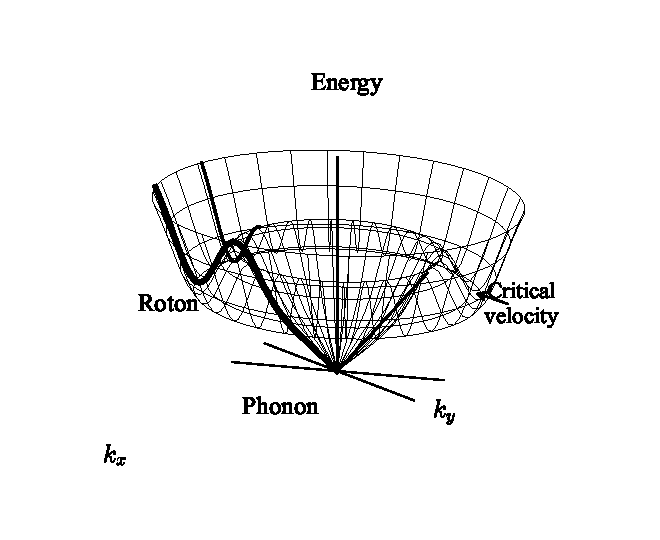
\includegraphics[width=0.72\textwidth]{fig_3.1.pdf}
\caption*{图 3.1\quad 声子激发位于 $\pmb{k}=0$ 附近，旋子激发位于有限 $\pmb{k}$ 处的局域极小附近。图中还标出了超流流动的临界速度（参见 3.7.3 节）。}
\end{figure}

然而，有一点是清楚的。平均场理论并不保证零能隙。要得到零能隙，我们只能依靠仔细的计算并祈盼奇迹。但是，从物理的角度看，无能隙激发的存在是一条普适原理，它不依赖于玻色系统的任何细节。无论相互作用取何种形式，自由空间中的玻色系统总是可压缩的，并且总含有无能隙的密度波。我们看到，平均场理论并没有把握住无能隙激发背后的原理。平均场理论的这个问题并不只出现在玻色系统中。一般而言，所有平均场理论都有这样的毛病：原理论的某些普遍原理没有被平均场理论捕捉到。在用平均场理论研究激发谱时，必须牢记这一点，并格外小心。

在真实的超流体中，激发谱具有图 3.1 所示的形状。位于有限 $\pmb{k}$ 处极小附近的激发称为旋子（roton）。我们注意到，在适当的 $\pmb{k}$ 处，旋子的群速度可以为零。

\subsection*{问题 3.2.1}

对于一个密度为 $\rho=N/\mathcal{V}$ 的一维相互作用玻色系统，确定 $N_0$ 与 $\mu$。证明一维的相互作用玻色子即使在零温下也不能凝聚。（注意，无相互作用的玻色子在零温下可以在一维凝聚。）

\subsection*{问题 3.2.2}

\begin{enumerate}
\item 找出一个 $V_{\pmb{k}}$，使得 $E_{\pmb{k}}$ 中的旋子极小降到零以下。在实空间中画出这个 $V(\pmb{x})$。
\item 当旋子极小果真降到零以下时，超流态会发生什么？
\end{enumerate}

\subsection*{问题 3.2.3}

自旋链的平均场理论。考虑自旋链
\begin{equation*}
H=J\sum_i S_iS_{i+1}
\end{equation*}
其中 $J<0$，$S$ 是携带自旋 $S$ 的自旋算符。当 $S\gg0$ 时，$S_i$ 的量子涨落很弱，我们可以把一个 $S$ 用其平均值 $s=\langle S_i\rangle$（假设它不依赖 $i$）代替，从而得到平均场哈密顿量。
\begin{enumerate}
\item 写出平均场哈密顿量，并求出平均场基态。
\item 用平均场哈密顿量计算 $\langle S_i\rangle$，从而确定 $s$ 的值。
\item 用平均场近似求出基态能量。
\item 求出平均场基态之上各激发的能量。
\end{enumerate}

我们由此看到，平均场理论完全无法重现无能隙的自旋波激发。2.4 节所讨论的路径积分方法及其经典近似则会给出好得多的结果。

\section{相互作用玻色系统的路径积分方法}

\subsection{相互作用玻色系统的路径积分表示}

如 3.1 节所述，自由玻色系统可以用一簇独立的谐振子来描述，其哈密顿量为
\begin{equation*}
H_0=\sum_{\pmb{k}}(\epsilon_{\pmb{k}}-\mu)a_{\pmb{k}}^{\dagger}a_{\pmb{k}}
\end{equation*}
这些谐振子（以及自由玻色系统）容许一个（相干态）路径积分表示
\begin{equation*}
\int\mathcal{D}^2\left[a_{\pmb{k}}(t)\right]\,\mathrm{e}^{\mathrm{i}\int \mathrm{d}t\,\sum_{\pmb{k}}\left[\mathrm{i}\frac{1}{2}(a_{\pmb{k}}^{*}\dot{a}_{\pmb{k}}-a_{\pmb{k}}\dot{a}_{\pmb{k}}^{*})-(\epsilon_{\pmb{k}}-\mu)a_{\pmb{k}}^{*}a_{\pmb{k}}\right]}
\end{equation*}
在实空间中，我们有
\begin{equation*}
\int\mathcal{D}^2a\;\mathrm{e}^{\mathrm{i}\int \mathrm{d}^d\pmb{x}\,\mathrm{d}t\,\left[\mathrm{i}\frac{1}{2}\left(a^{*}(\pmb{x},t)\partial_t a(\pmb{x},t)-a(\pmb{x},t)\partial_t a^{*}(\pmb{x},t)\right)-\frac{1}{2m}\partial_{\pmb{x}}a^{*}(\pmb{x},t)\partial_{\pmb{x}}a(\pmb{x},t)-\mu a^{*}(\pmb{x},t)a(\pmb{x},t)\right]}
\end{equation*}
现在我们可以很容易地把相互作用包括进来，只需在哈密顿量与路径积分中加上一项
\begin{equation*}
\int \mathrm{d}^d\pmb{x}\,\mathrm{d}^d\pmb{y}\;\frac{1}{2}a^{*}(\pmb{x},t)a(\pmb{x},t)V(\pmb{x}-\pmb{y})a^{*}(\pmb{y},t)a(\pmb{y},t)
\end{equation*}
这里我们将处理一个更简单的相互作用 $V(\pmb{x})=V_0\delta(\pmb{x})$，其傅里叶分量为 $V_{\pmb{k}}=V_0$。相互作用玻色子的路径积分于是具有形式
\begin{equation*}
\int\mathcal{D}^2\left[\varphi(\pmb{x},t)\right]\,\mathrm{e}^{\mathrm{i}\int \mathrm{d}^d\pmb{x}\,\mathrm{d}t\,\left[\mathrm{i}\frac{1}{2}(\varphi^{*}\partial_t\varphi-\varphi\partial_t\varphi^{*})-\frac{1}{2m}\partial_{\pmb{x}}\varphi^{*}\partial_{\pmb{x}}\varphi+\mu|\varphi|^2-\frac{V_0}{2}|\varphi|^4\right]}
\end{equation*}
其中，按照惯例，我们已把 $a(\pmb{x},t)$ 改记为 $\varphi(\pmb{x},t)$。

\begin{figure}[H]
\centering
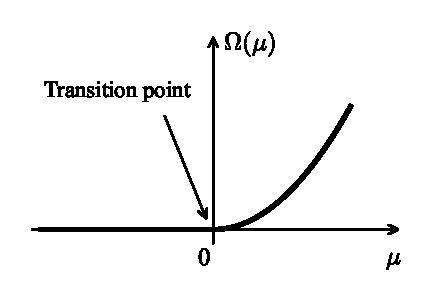
\includegraphics[width=0.72\textwidth]{fig_3.2.pdf}
\caption*{图 3.2\quad 热势 $\Omega(\mu)$ 的二阶导数出现不连续，这标志着一次二级相变。}
\end{figure}

有了路径积分表示，我们就可以把这个量子相互作用玻色系统当作一个经典场论来研究其物理性质，该经典场论由作用量
\begin{equation*}
S=\int \mathrm{d}^d\pmb{x}\,\mathrm{d}t\,\left[\mathrm{i}\frac{1}{2}(\varphi^{*}\partial_t\varphi-\varphi\partial_t\varphi^{*})-\frac{1}{2m}\partial_{\pmb{x}}\varphi^{*}\partial_{\pmb{x}}\varphi+\mu|\varphi|^2-\frac{V_0}{2}|\varphi|^4\right]\tag{3.3.1}
\end{equation*}
描述。这里我们做的是半经典近似（而不是 3.2 节所做的平均场近似），其领头项就是经典理论。这个经典系统的能量（或者，更准确地说，热势）为
\begin{equation*}
\Omega=\int \mathrm{d}^d\pmb{x}\,\left[\frac{1}{2m}\partial_{\pmb{x}}\varphi^{*}\partial_{\pmb{x}}\varphi+\mu|\varphi|^2+\frac{V_0}{2}|\varphi|^4\right]\tag{3.3.2}
\end{equation*}

\subsection{相变与自发对称性破缺}

\begin{keypoints}
\item 零温相变发生在基态能量的非解析点处。
\item 当一个非对称的基态从对称系统中涌现时，就发生了自发对称性破缺。
\item 连续相变、自发对称性破缺与长程序密切相关。这正是 Landau 关于相与相变的对称性破缺理论的核心。
\end{keypoints}

经典基态是平移不变的，由一个复常数 $\varphi_0$ 刻画：$\varphi(\pmb{x},t)=\varphi_0$。经典基态的能量密度（或者，更准确地讲，是热势的密度）为

% ------------------------------------------------------------
% 块边界备注：
%   终点：书页 78（p093）末句 "The energy density (or, more precisely, the
%   density of the thermal potential) of the classical ground state is"
%   跨页延续到书页 79（p094）顶部。p094 顶部残句 "density of the thermal
%   potential) ..." 的译文（"密度）为"）已按任务约定写入本文件顶部
%   %--A-TAIL-- 区。ch3_b 请勿重复翻译该残句，正文请从 p094 的无编号式
%   Ω_0/𝒱 = −μ|φ_0|² + (V_0/2)|φ_0|⁴ 起译（其后为 "By minimizing the
%   energy..." 一段）。
%   另：本块含 §3.3 与 §3.3.1 的开头、§3.3.2 的标题＋要点＋首句（未完）。
% ------------------------------------------------------------
% 新增术语（ch3_a，待并入术语表"新增术语"区）：
%   first quantization 第一次量子化
%   normal ordering 正规排序
%   c-number c 数
%   boson condensed state 玻色凝聚态
%   chemical potential 化学势
%   dispersion relation 色散关系
%   off-diagonal long-range order 非对角长程序
%   trial wave function 尝试波函数
%   phonon 声子
%   roton 旋子
%   critical velocity 临界速度
%   group velocity 群速度
%   density wave 密度波
%   Nambu–Goldstone modes Nambu–Goldstone 模
%   second-order phase transition 二级相变
%   classical field theory 经典场论
%   Fourier component 傅里叶分量
%   spin chain 自旋链
%   spin wave 自旋波
%   weak-coupling limit 弱耦合极限
%   low-density limit 低密度极限
\begin{equation*}
\frac{\Omega_0}{\mathcal{V}} = -\mu|\varphi_0|^2 + \frac{V_0}{2}|\varphi_0|^4
\end{equation*}

\begin{figure}[H]
\centering
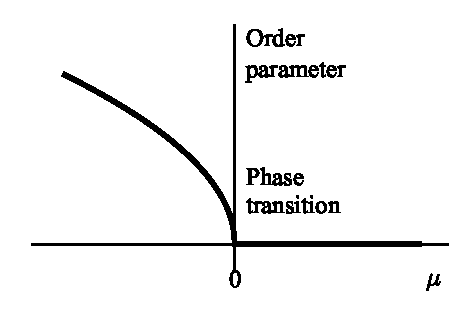
\includegraphics[width=0.72\textwidth]{fig_3.3.pdf}
\caption*{图 3.3\quad 序参量 $\varphi_0$ 与超流相变。}
\end{figure}

对能量求极小，我们看到，对于 $\mu < 0$，基态由 $\varphi_0 = 0$ 表征，对应于没有玻色子的态。对于 $\mu > 0$，基态是简并的，由玻色场的下列幅值表征：
\begin{equation*}
\varphi_0 = \sqrt{\frac{\mu}{V_0}}\,\mathrm{e}^{\mathrm{i}\theta}\tag{3.3.3}
\end{equation*}
其中 $\theta$ 可任取。这样的态具有玻色子密度 $\rho_0 = \mu/V_0$。热势作为 $\mu$ 的函数由下式给出：
\begin{equation*}
\Omega_0(\mu) =
\begin{cases}
0, & \text{当 } \mu < 0\\[6pt]
\dfrac{\mu^2}{V_0}, & \text{当 } \mu > 0
\end{cases}
\end{equation*}
（译注：由上一式可得 $\mu>0$ 时 $\Omega_0/\mathcal{V} = -\mu^2/(2V_0)$；原书此处印作 $\mu^2/V_0$，未含体积 $\mathcal{V}$ 与因子 $-1/2$，疑为排印之误。）

我们看到，作为 $\mu$ 的函数，基态能量 $\Omega_0(\mu)$ 在 $\mu = 0$ 处有一个奇点。该奇点标志着 $\mu = 0$ 处的一个二级相变，因为 $\Omega_0''(\mu)$ 在该点有一跳变（见图 3.2）。这个相变称为超流相变（superfluid transition）。\footnote{我们将在 3.7.3 节讨论超流性。}

超流相的特征是非零的玻色场 $\varphi(\pmb{x}) \neq 0$，而无玻色子相的特征是玻色场为零 $\varphi(\pmb{x}) = 0$。超流相变由 $\varphi_0 = 0$ 到 $\varphi_0 \neq 0$ 的改变所标志（见图 3.3）。因此，我们称 $\varphi_0$ 为超流的序参量。

超流相还以对称性破缺为特征。我们看到，我们的哈密顿量或拉格朗日量具有 $U(1)$ 对称性，因为在变换
\begin{equation*}
\varphi \rightarrow \mathrm{e}^{\mathrm{i}\theta}\varphi\tag{3.3.4}
\end{equation*}
之下，无论我们处于哪个相，它们都保持不变。然而，超流相中的（经典）基态（见式 (3.3.3)）不尊重 $U(1)$ 对称性，也就是说，它们在 $U(1)$ 变换 (3.3.4) 下不是不变的。

\begin{figure}[H]
\centering
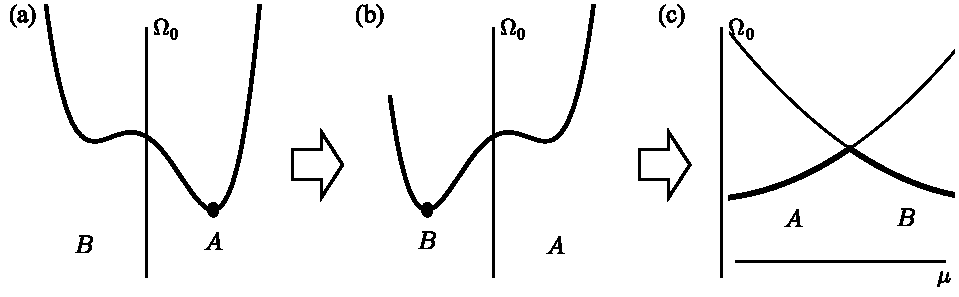
\includegraphics[width=0.72\textwidth]{fig_3.4.pdf}
\caption*{图 3.4\quad (a)与(b)：在不同极小值之间的切换导致(c)中 $\Omega_0$ 的一个拐折，它代表一个一级相变。}
\end{figure}

\begin{figure}[H]
\centering
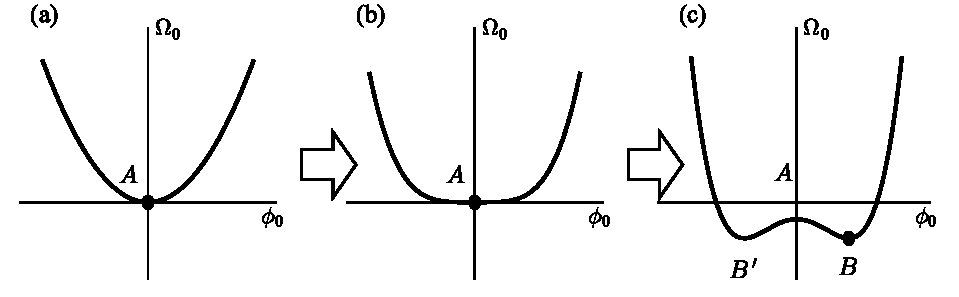
\includegraphics[width=0.72\textwidth]{fig_3.5.pdf}
\caption*{图 3.5\quad 在存在 $\phi_0 \to -\phi_0$ 对称性时，极小值之间的切换可以连续地进行，并导致一个二级相变。(a)基态在 $\phi_0 \to -\phi_0$ 条件下是对称的。(b)转变点。(c)基态破坏 $\phi_0 \to -\phi_0$ 对称性。}
\end{figure}

超流相变展示了一条深刻的原理：以热势 $\Omega$ 的非解析点为特征的连续相变，与态的对称性的改变相关联。为领会这一点，让我们从头说起。我们知道，相变是由系统的能量或自由能中的奇点引起的。所以，要理解相变，就需要理解（自由）能是如何产生奇点的。

对于相互作用玻色系统，能量函数 $\Omega_0(\mu; \phi_0)$ 作为 $\phi_0$ 和 $\mu$ 的函数是一个没有奇点的解析函数。基态能量 $\Omega_0(\mu)$ 是 $\Omega_0(\mu; \phi_0)$ 对 $\phi_0$ 取的极小值。一般地，$\Omega_0(\mu)$ 也是解析函数。然而，有时 $\Omega_0(\mu; \phi_0)$ 作为 $\phi_0$ 的函数有多个局部极小。当我们改变 $\mu$ 时，全局极小可能从一个局部极小切换到另一个（见图 3.4）。在这种情况下，所得的 $\Omega_0(\mu)$ 将在切换点有一个奇点。这样的奇点代表一个一级相变，因为 $\Omega_0'(\mu)$ 有一跳变（见图 3.4(c)）。

然而，当能量函数 $\Omega_0(\mu,\phi_0)$ 具有对称性，比如说 $\Omega_0(\mu,\phi_0) = \Omega_0(\mu,\mathrm{e}^{\mathrm{i}\theta}\phi_0)$ 时，极小值之间的切换可以有非常不同的行为，并且可以是连续的（见图 3.5）。由于这一对称性，新的全局极小是简并的。系统面临一个艰难的抉择：要挑哪一个极小驻留。系统做出选择之后，新相便不再具有 $\phi_0 \to \mathrm{e}^{\mathrm{i}\theta}\phi_0$ 对称性。这种从对称系统中演生出非对称态的现象称为自发对称性破缺。我们看到，二级相变与基态对称性的改变密切相关。这正是 Landau 相与相变对称性破缺理论的核心（Landau, 1937）。这一简单的思想应用极为广泛。实际上，几乎所有连续相变都以某种自发对称性破缺为特征。

一般地，自发对称性破缺可以用一个序参量来表征。序参量可以选为一个在对称变换下非平凡变换的算符的期望值。在上面，我们选 $\langle\varphi\rangle$ 作为序参量。由于其变换性质 $\langle\varphi\rangle \to \mathrm{e}^{\mathrm{i}\theta}\langle\varphi\rangle$，在对称相中 $\langle\varphi\rangle = 0$。相比之下，在对称性破缺相中 $\langle\varphi\rangle = \varphi_0 \neq 0$。

在对称性破缺相中，如果我们知道 $\varphi$ 场在一点的相位，那么我们就知道它在任何其他点的相位。这一性质称为长程序。$\varphi$ 场中的长程关联可以在数学上表示为
\begin{equation*}
\left.\left\langle \varphi(t,\pmb{x})^{\dagger}\varphi(0,0)\right\rangle\right|_{(t,\pmb{x})\to\infty} = |\varphi_0|^2 \neq 0
\end{equation*}
如果 $\varphi$ 的相位在各点之间是无规且互不关联的，那么上述关联将为零。当然，这里我们只考虑没有量子涨落的经典基态。在这种情形下我们看到，非零序参量与 $\varphi$ 算符中的长程序密切相关。对称性破缺相既可以用非零序参量表征，也可以用长程关联表征。在下面几节中，我们将把量子涨落包括进来，看看它们会如何影响序参量和长程序。

\subsection*{问题 3.3.1}

由作用量 (3.3.1) 导出经典运动方程。只考虑基态附近的小涨落，对对称相（$\mu < 0$）与对称性破缺相（$\mu > 0$）分别导出线性化的运动方程。证明对称基态附近的涨落具有有限能隙，而对称性破缺基态附近的涨落包含一个零能隙的模式。此模式具有线性色散 $\omega \propto k$。

\subsection*{问题 3.3.2}

水–水蒸气相变可以用下列吉布斯能（Gibbs energy）函数描述：
\begin{equation*}
G(T,P;n) = h(T,P)n + a(T,P)n^2 + c(T,P)n^3 + b(T,P)n^4
\end{equation*}
其中 $n$ 是水分子的密度。系统的吉布斯能 $G(T,P)$ 由 $G(T,P;n)$ 对 $n$ 取极小值给出。系统有一条一级相变线，它终止于一个临界点。试求确定一级相变线与临界点的方程。（提示：先考虑 $c = 0$ 的情形。如果把 $n$ 看作自旋矩的密度，这样的吉布斯能与磁场 $\delta\rho$ 中伊辛模型的自由能具有相同的形式。）

\subsection{低能有效理论}

\begin{keypoints}
\item 描述慢（即低能）涨落的有效拉格朗日量，可以通过积掉快（即高能）涨落得到。
\end{keypoints}

为研究经典基态之上的激发，让我们考虑经典基态附近的下述小涨落：
\begin{equation*}
\varphi = \varphi_0 + \delta\varphi
\end{equation*}
$\delta\varphi$ 的动力学由同一个作用量 (3.3.1) 支配。但现在我们可以假设 $\delta\varphi$ 很小，只保留 $\delta\varphi$ 的二次项。对于对称相 $\varphi_0 = 0$，我们有
\begin{equation*}
S = \int \mathrm{d}^d\pmb{x}\,\mathrm{d}t\,\Big[\mathrm{i}\frac{1}{2}(\varphi^*\partial_t\varphi - \varphi\partial_t\varphi^*) - \frac{1}{2m}\partial_{\pmb{x}}\varphi^*\,\partial_{\pmb{x}}\varphi + \mu\varphi^*\varphi\Big]\tag{3.3.5}
\end{equation*}
在对称相中，运动方程为
\begin{equation*}
\Big[\mathrm{i}\partial_t - \frac{1}{2m}(-\mathrm{i}\partial_{\pmb{x}})^2 + \mu\Big]\varphi = 0
\end{equation*}
由此得到涨落的如下色散：
\begin{equation*}
\omega = \frac{1}{2m}k^2 - \mu\tag{3.3.6}
\end{equation*}
在下一节中我们将看到，这些涨落对应于类粒子激发：涨落的频率与波矢量分别变成粒子的能量与动量。我们看到，激发具有有限能隙 $\Delta = -\mu$（注意 $\mu < 0$），这正是产生一个激发所需的能量。事实上，由色散 (3.3.6) 所描述的粒子恰好对应于构成我们系统的那些玻色子。

为理解对称性破缺相中的低能激发，我们希望推导一个只包含与低能激发相关的模式的低能有效理论。至于哪些涨落具有低能量，我们注意到，在对称性破缺相中，凝聚体的不同相位 $\theta$ 导致简并的基态。如果我们在一个很大但有限的区域内改变凝聚体的相位，那么系统在局部上仍处于它的某个简并基态。系统得以知道自己处于激发态的唯一途径是通过 $\theta$ 的梯度。如果相位在空间中变化缓慢，相应的激发就具有较小的能量。因此，低能激发对应于诸简并基态之间的涨落，由 $\theta$ 场描述。基于这一图像，我们写出
\begin{equation*}
\varphi = \sqrt{\rho_0 + \delta\rho}\,\mathrm{e}^{\mathrm{i}\theta}\tag{3.3.7}
\end{equation*}
其中 $\rho_0 = \varphi_0^2 = \mu/V_0$ 是基态的密度，$\delta\rho$ 是密度涨落。在这种写法中，$\theta$ 描述低能的慢涨落，$\delta\rho$ 描述高能的快涨落。把式 (3.3.7) 代入式 (3.3.1)，并展开到 $\theta$ 与 $\delta\rho$ 的二次阶，我们得到
\begin{equation*}
S = \int \mathrm{d}^d\pmb{x}\,\mathrm{d}t\,\Big[-(\rho_0+\delta\rho)\partial_t\theta - \frac{\rho_0(\partial_{\pmb{x}}\theta)^2}{2m} - \frac{(\partial_{\pmb{x}}\delta\rho)^2}{8m\rho_0} - \frac{V_0}{2}\delta\rho^2\Big]\tag{3.3.8}
\end{equation*}

这里我们面对的是多体物理中一个十分典型的问题。我们有两个场，一个描述慢的低频（即低能）涨落，另一个描述快的高频涨落。如果我们只关心低能物理，如何移除快场，以得到一个简单的低能有效理论？

得到低能有效理论的一种办法是令 $\delta\rho = 0$，把 $\delta\rho$ 场丢掉。这导致 $\theta$ 的下列低能有效作用量：
\begin{equation*}
S = \int \mathrm{d}^d\pmb{x}\,\mathrm{d}t\,\Big[-\varphi_0^2\partial_t\theta - \frac{1}{2m}\varphi_0^2(\partial_{\pmb{x}}\theta)^2\Big]
\end{equation*}
然而，这个有效作用量并不十分正确，因为 $\partial_t\theta$ 是一个全导数（total derivative），它不进入运动方程。我们需要得到 $(\partial_t\theta)^2$ 项，才能理解 $\theta$ 的低能动力学性质。要得到 $(\partial_t\theta)^2$ 项，移除 $\delta\rho$ 场时就必须更加小心。

得到低能有效理论的一个更好的办法，是在路径积分中积分掉快场 $\delta\rho$。在这里这很容易做到，因为作用量 (3.3.8) 是 $\delta\rho$ 的二次型。完成高斯积分后，我们发现
\begin{align*}
Z &= \int \mathcal{D}\theta\,\mathrm{e}^{\mathrm{i}\int \mathrm{d}^d\pmb{x}\,\mathrm{d}t\,\big[-\frac{\rho_0}{2m}(\partial_{\pmb{x}}\theta)^2 + \frac{1}{2}\partial_t\theta\,\frac{1}{V_0 - \frac{1}{4m\rho_0}\partial_{\pmb{x}}^2}\,\partial_t\theta\big]}\\
&\approx \int \mathcal{D}\theta\,\mathrm{e}^{\mathrm{i}\int \mathrm{d}^d\pmb{x}\,\mathrm{d}t\,\big[-\frac{\rho_0}{2m}(\partial_{\pmb{x}}\theta)^2 + \frac{1}{2V_0}(\partial_t\theta)^2\big]}\tag{3.3.9}
\end{align*}
其中我们假设了 $\theta$ 场在空间中变化缓慢，并丢掉了 $\frac{1}{4m\rho_0}(\partial_{\pmb{x}})^2$ 项；我们还丢掉了作用量中的全时间导数项。\footnote{在存在涡旋时，全时间导数项是重要的，那时不应将其丢掉。见 3.6 节。}我们得到 $\theta$ 的下列简单的低能有效作用量：
\begin{equation*}
S_{\mathrm{eff}} = \int \mathrm{d}^d\pmb{x}\,\mathrm{d}t\,\Big[\frac{1}{2V_0}(\partial_t\theta)^2 - \frac{\rho_0}{2m}(\partial_{\pmb{x}}\theta)^2\Big]\tag{3.3.10}
\end{equation*}
注意 $\theta$ 场实际上生活在一个圆上，因此 $\theta$ 与 $\theta + 2\pi$ 描述同一点。为更准确起见，我们可以引入 $z = \mathrm{e}^{\mathrm{i}\theta}$，把上式改写为
\begin{equation*}
S_{\mathrm{eff}} = \int \mathrm{d}^d\pmb{x}\,\mathrm{d}t\,\Big[\frac{1}{2V_0}|\partial_t z|^2 - \frac{\rho_0}{2m}|\partial_{\pmb{x}} z|^2\Big]\tag{3.3.11}
\end{equation*}
由式 (3.3.10) 或式 (3.3.11) 所描述的模型称为 XY 模型（XY-model）。

经典基态由均匀的 $\theta$ 场给出：$\theta(\pmb{x},t) = $ 常数。激发由 $\theta$ 的涨落描述，这些涨落满足运动方程
\begin{equation*}
\Big(-\frac{1}{2V_0}\partial_t^2 + \frac{\rho_0}{2m}\partial_{\pmb{x}}^2\Big)\theta = 0
\end{equation*}
上式是一个波动方程，它描述一列具有线性色散的波
\begin{equation*}
\omega = v|\pmb{k}|,\qquad v^2 = \frac{\rho_0 V_0}{m}\tag{3.3.12}
\end{equation*}
其中 $v$ 是波速。

在许多情形下，仅仅知道低能有效作用量是不够的。同样重要的是要知道，原理论中的场（或算符）如何由低能有效理论中的场（或算符）来表示。下面我们以密度算符为例，说明原理论中的物理算符（或场）如何由有效理论中的场来表示。首先，在原拉格朗日量中加一个与密度耦合的源项 $-A_0\rho = -A_0(\rho_0 + \delta\rho)$。然后，进行同样的计算以得到有效理论。我们发现，有效理论中含有一个附加项（准确到 $A_0$ 的线性阶）$-A_0(\rho_0 - \frac{\partial_t\theta}{V_0})$。于是，密度算符在有效理论中表示为
\begin{equation*}
\rho = \rho_0 - \frac{\partial_t\theta}{V_0}\tag{3.3.13}
\end{equation*}
类似地，我们发现玻色子流密度 $\pmb{j} = \mathrm{Re}\,\varphi^{\dagger}\frac{\partial_{\pmb{x}}}{\mathrm{i}m}\varphi$ 在有效理论中变为
\begin{equation*}
\pmb{j} = \frac{\rho_0}{m}\partial_{\pmb{x}}\theta\tag{3.3.14}
\end{equation*}
式 (3.3.13)、式 (3.3.14) 与式 (3.3.10) 使我们能够在简单的低能有效理论之内，用路径积分计算密度关联与流关联。这些关联随后便可与诸如压缩率（compressibility）和电导率等实验结果相比较。$\rho$ 与 $\theta$ 之间的关系还告诉我们，$\theta$ 所描述的低能涨落正是密度–流涨落。

\subsection*{问题 3.3.3}

\begin{enumerate}
\item[(a)] 得到 $\theta$ 的低能有效理论还有另一种办法：通过求解 $\delta\rho$ 场的运动方程，把 $\delta\rho$ 用 $\partial_t\theta$、$\partial_{\pmb{x}}\theta$ 等表示出来；然后把 $\delta\rho$ 代回作用量，得到一个只含 $\theta$ 的有效作用量。证明这一方法给出同样的 XY 模型作用量 (3.3.10)。
\item[(b)] 如果把 $\delta\rho$ 代入密度算符和流算符，则会分别重新得到式 (3.3.13) 与式 (3.3.14)。证明 $\rho$ 和 $\pmb{j}$ 满足守恒定律 $\partial_t\rho + \partial_{\pmb{x}}\cdot\pmb{j} = 0$。
\item[(c)] 用式 (3.3.13) 给出的密度算符表达式，计算动量–频率空间中超流的密度–密度关联函数。
\end{enumerate}

\subsection{波即是粒子}

\begin{keypoints}
\item 超流态中演生出一种新型的粒子——准粒子（quasiparticle）。准粒子是玻色型的、无相互作用的，并且具有线性色散。
\end{keypoints}

我们一直把经典基态附近的 $\theta$ 涨落（或者对称相中的 $\delta\varphi$）看作波。由于量子物理中的波粒二象性（particle–wave duality），波也可以看作粒子。这些粒子称为准粒子。下面我们将量子化低能有效理论，得到准粒子的量子理论。该量子理论结果是一个玻色子理论，这告诉我们准粒子是玻色子。

我们先把低能有效拉格朗日量 (3.3.10) 在 $\pmb{k}$ 空间中写成如下形式：
\begin{equation*}
L_{\mathrm{eff}} = \sum_{\pmb{k}}\Big[\frac{A_{\pmb{k}}}{2}\dot{\theta}_{-\pmb{k}}\dot{\theta}_{\pmb{k}} - \frac{B_{\pmb{k}}}{2}\theta_{-\pmb{k}}\theta_{\pmb{k}}\Big],\tag{3.3.15}
\end{equation*}
其中
\begin{equation*}
A_{\pmb{k}} = V_0^{-1},\qquad B_{\pmb{k}} = \frac{\rho_0 k^2}{m},\tag{3.3.16}
\end{equation*}
$\theta_{\pmb{k}} = \mathcal{V}^{-1/2}\int \mathrm{d}^d\pmb{x}\,\theta(\pmb{x})\mathrm{e}^{-\mathrm{i}\pmb{k}\cdot\pmb{x}}$，而 $\mathcal{V}$ 是系统的总体积。上述作用量描述一组彼此退耦的谐振子。

为得到描述量子化理论的量子哈密顿量，我们先算出经典哈密顿量。$\theta_{\pmb{k}}$ 的正则动量（canonical momentum）为
\begin{equation*}
\pi_{\pmb{k}} = \frac{\partial L_{\mathrm{eff}}}{\partial \dot{\theta}_{\pmb{k}}} = A_{\pmb{k}}\dot{\theta}_{-\pmb{k}}
\end{equation*}
经典哈密顿量 $H = \sum_{\pmb{k}}\pi_{\pmb{k}}\dot{\theta}_{\pmb{k}} - L_{\mathrm{eff}}$ 由下式给出：
\begin{equation*}
H = \sum_{\pmb{k}}\Big[\frac{1}{2A_{\pmb{k}}}\pi_{-\pmb{k}}\pi_{\pmb{k}} + \frac{B_{\pmb{k}}}{2}\theta_{-\pmb{k}}\theta_{\pmb{k}}\Big]
\end{equation*}
只需把 $\pi_{\pmb{k}}$ 和 $\theta_{\pmb{k}}$ 当作满足下列正则对易关系（canonical commutation relation）的算符，就得到量子哈密顿量：
\begin{equation*}
[\theta_{\pmb{k}}, \pi_{\pmb{k}'}] = \mathrm{i}\delta_{\pmb{k}\pmb{k}'}
\end{equation*}
现在我们引入
\begin{equation*}
\alpha_{\pmb{k}} = u_{\pmb{k}}\theta_{\pmb{k}} + \mathrm{i}v_{\pmb{k}}\pi_{-\pmb{k}},\quad u_{\pmb{k}} = \frac{1}{\sqrt{2}}(A_{\pmb{k}}B_{\pmb{k}})^{1/4},\quad v_{\pmb{k}} = \frac{1}{\sqrt{2}}(A_{\pmb{k}}B_{\pmb{k}})^{-1/4}.\tag{3.3.17}
\end{equation*}
我们发现 $\alpha_{\pmb{k}}$ 满足振子下降算符（lowering operator）的代数：
\begin{equation*}
[\alpha_{\pmb{k}}, \alpha_{\pmb{k}'}^{\dagger}] = \delta_{\pmb{k}\pmb{k}'},\qquad [\alpha_{\pmb{k}}, \alpha_{\pmb{k}'}] = 0.
\end{equation*}
用下降与上升算符（raising operator）$(\alpha_{\pmb{k}}, \alpha_{\pmb{k}}^{\dagger})$ 表示，哈密顿量取振子的标准形式：
\begin{equation*}
H = \sum_{\pmb{k}}\epsilon_{\pmb{k}}\alpha_{\pmb{k}}^{\dagger}\alpha_{\pmb{k}} + \text{常数},\qquad \epsilon_{\pmb{k}} = \sqrt{\frac{B_{\pmb{k}}}{A_{\pmb{k}}}} = \sqrt{\frac{V_0\rho_0}{m}}\,|\pmb{k}| = v|\pmb{k}|\tag{3.3.18}
\end{equation*}
这正是具有单玻色子能量 $\epsilon_{\pmb{k}} = v|\pmb{k}|$ 的自由玻色子哈密顿量 (3.1.1)。

我们看到，$\theta$ 的集体涨落产生了具有线性色散的玻色型准粒子。由于 $\theta$ 的涨落对应于超流体中的密度波，我们也可以说，密度波在量子理论中变成了离散的准粒子。这一图像适用于更普遍的情形。事实上，量子基态的任何波状涨落在量子化之后都对应于离散的准粒子。\footnote{空气中的声波不对应于任何离散的准粒子。这是因为声波不是任何量子基态的涨落，因此它不对应于基态之上的任何激发。}固体中的声波变成由哈密顿量 (3.3.18) 描述的声子（phonon）。因此，我们也将把超流体中的准粒子称作声子。声子速度（即密度波的速度）$v = \sqrt{V_0\rho_0/m}$ 与平均场结果 (3.2.9) 相一致。

我们想强调，玻色型准粒子——声子——与构成超流体的原来那些玻色子截然不同。原来的玻色子具有二次色散 $\epsilon_{\pmb{k}} = k^2/2m$，而声子具有线性色散 $\epsilon_{\pmb{k}} = v|\pmb{k}|$；原来的玻色子是有相互作用的，而声子是自由的。事实上，一个声子对应于许多原来玻色子的一种集体运动。这是从相互作用玻色系统中演生出一种新型玻色子——具有线性色散的无相互作用声子——的一个例子。

\subsection{作为玩具宇宙的超流体}

\begin{keypoints}
\item 如果我们把超流体看作一个玩具宇宙，那么声子将是这个玩具宇宙中无质量的“基本粒子”。
\item 旋子（roton，即涡环 vortex ring）可以通过交换声子发生相互作用。这导致两个旋子之间的 $1/r^4$ 偶极相互作用。
\end{keypoints}

为了领会我们的宇宙以及其中的基本粒子，让我们想象一个由超流体形成的玩具宇宙（toy universe）。假设构成超流体的玻色子太小，玩具宇宙中的居民看不见它们。问题是：在玩具宇宙的居民看来，这个玩具宇宙是什么样子的？

\begin{figure}[H]
\centering
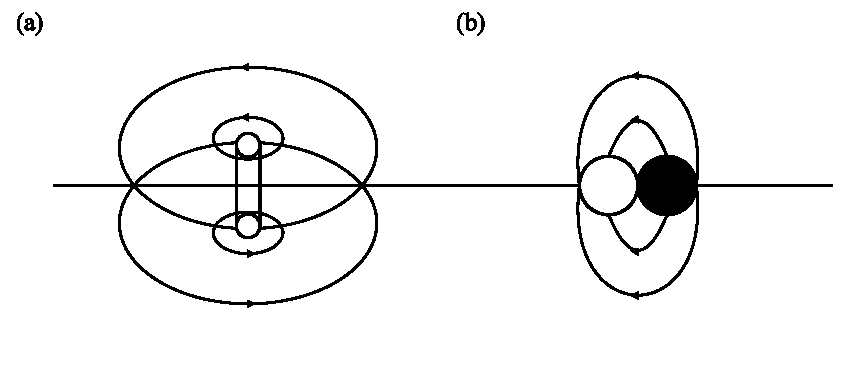
\includegraphics[width=0.72\textwidth]{fig_3.6.pdf}
\caption*{图 3.6\quad (a)旋子（涡环）周围与(b)声子电荷的偶极子周围的玻色子流动图案。}
\end{figure}

这个玩具宇宙包含一种无质量激发\footnote{质量为 $m$ 的相对论性粒子具有色散 $\epsilon_{\pmb{k}} = \sqrt{m^2c^4 + c^2\pmb{k}^2}$，其中 $c$ 是光速。声子色散 $\epsilon_{\pmb{k}} = v|\pmb{k}|$ 可以看作 $\sqrt{m^2c^4 + c^2\pmb{k}^2}$ 的无质量极限，其中声子速度 $v$ 扮演光速的角色。}——声子。对玩具宇宙中的居民来说，声子只是一种类粒子激发，因为没有人能看见构成超流体的玻色子，也没有人知道声子从何而来。于是，玩具宇宙的居民便把声子称作一种“基本粒子”。

我们看到，这个玩具宇宙与我们的宇宙十分相似。我们的宇宙也有一种无质量激发——光子。我们也把光子称作“基本粒子”。与声子一样，光子彼此之间也不相互作用。然而，电荷之间的 $1/r^2$ 库仑定律正是由光子传递的。那么，声子是否也会在它们的“电荷”之间诱导出类似的相互作用呢？

上述问题的答案是肯定的。不过，我们首先需要解释声子的“电荷”是什么。我们知道，电荷产生守恒的通量——电场。类似地，声子的“电荷”也产生守恒的通量，只不过对声子而言，这个通量是超流体中玻色子的通量。按定义，一个正的“声子电荷”（phonon charge）是玻色子的源：玻色子在某个点以恒定速率被产生；一个负的声子电荷则是玻色子的汇：玻色子在某个点以恒定速率被湮没。

为理解声子电荷之间的相互作用，我们对满足约束 $\partial_{\pmb{x}}\cdot\pmb{j} \allowbreak- J^0 = 0$ 的 $\theta$ 极小化能量 $\int \mathrm{d}^3\pmb{x}\,\allowbreak\frac{\rho_0}{2m}(\partial_{\pmb{x}}\theta)^2$。这里 $\pmb{j} = \frac{\rho_0}{m}\partial_{\pmb{x}}\theta$ 是玻色子流，$J^0(\pmb{x},t) = \sum_i q_i\delta(\pmb{x} - \pmb{x}_i)$ 是声子电荷的密度，$q_i$ 是第 $i$ 个声子电荷的值。$q_i > 0$ 对应于源，$q_i < 0$ 对应于汇。我们发现，两个声子电荷 $q_1$ 与 $q_2$ 之间的势正比于 $q_1q_2/r$。声子电荷之间的相互作用与库仑定律非常相似：力正比于 $1/r^2$，同号电荷相斥，异号电荷相吸。

在真实的超流体中，玻色子是守恒的。因此，源和汇——亦即声子电荷——是不允许存在的。唯一允许的激发是低能声子与高能旋子（见图 3.1）。应当注意，旋子可以看作由涡线（vortex line）构成的一个小环。\footnote{$(2+1)$ 维超流体中的涡旋定义见 3.4.2 节。这一定义可以推广到任意维度。}如果做多极展开（multipole expansion），旋子周围玻色子的流动图案可以看作由一组声子电荷产生的流动图案。玻色子数守恒要求多极展开中的声子电荷总和为零。涡环的对称性允许多极展开中存在有限的偶极矩（见图 3.6），而旋子的偶极矩一般不为零。因此，旋子彼此之间存在 $1/r^4$ 偶极相互作用。

总而言之，这个玩具宇宙包含带有偶极矩的粒子，其长程偶极相互作用通过交换无质量的声子而产生。

\subsection{自发对称性破缺与无能隙激发}

\begin{keypoints}
\item 普适性质（universal properties）的概念。
\item 连续对称性的自发破缺总是导致无能隙的玻色型激发。
\end{keypoints}

我们想强调，在超流体中，声子的三个性质——无相互作用、无能隙的线性色散以及玻色统计——是普适性质，不依赖于玻色子之间相互作用的细节。在上面，我们假设玻色子具有 $\delta$ 函数相互作用。然而，只要相互作用 $V(\pmb{x}-\pmb{x}')$ 是短程的，即使玻色子具有更一般的相互作用 $L_{int} = -\int \mathrm{d}\pmb{x}\,\mathrm{d}\pmb{x}'\,\frac{1}{2}|\varphi(\pmb{x})|^2 V(\pmb{x}-\pmb{x}')|\varphi(\pmb{x}')|^2$，这些普适性质也保持不变。既然准粒子的无能隙性是不依赖于初始拉格朗日量细节的普适性质，就应当存在着一种不依赖这些细节的关于无能隙性的一般性理解。事实表明，超流相中无能隙激发的存在，与拉格朗日量的 $U(1)$ 对称性以及基态的自发对称性破缺密切相关。下面我们将解释这一关系。

拉格朗日量 (3.3.1) 具有 $U(1)$ 对称性，因为它在 $U(1)$ 变换 $\varphi \to \mathrm{e}^{\mathrm{i}\eta}\varphi$ 下不变。如果我们显式破缺这一对称性，即使拉格朗日量不再尊重 $U(1)$ 对称性，低能模式也将获得有限能隙。例如，若在拉格朗日量中加入 $C\,\mathrm{Re}\varphi$ 项以显式破缺 $U(1)$ 对称性，则 XY 模型中会诱导出 $\cos(\theta)$ 形式的项：$\mathcal{L} = \frac{1}{2V_0}(\partial_t\theta)^2 - \frac{\rho_0}{2m}(\partial_{\pmb{x}}\theta)^2 + g\cos(\theta)$。经典基态由 $\theta = 0$ 给出。对于基态附近的小涨落，拉格朗日量可以简化为 $\mathcal{L} = \frac{1}{2V_0}(\partial_t\theta)^2 - \frac{\rho_0}{2m}(\partial_{\pmb{x}}\theta)^2 - \frac{g}{2}\theta^2$。所得的波动方程 $(-\frac{1}{2V_0}\partial_t^2 + \frac{\rho_0}{2m}\partial_{\pmb{x}}^2 - g)\theta = 0$ 告诉我们，无论波矢量如何，波总有有限频率 $\omega = \sqrt{2V_0g + \frac{V_0\rho_0}{m}k^2}$。于是，势项 $\cos(\theta)$ 为 $\theta$ 准粒子打开了一个能隙。

如果拉格朗日量和基态在 $U(1)$ 变换下都不变，那么对称性就没有破缺。由式 (3.3.6) 我们看到，对称基态一般也具有有限能隙。

\begin{figure}[H]
\centering
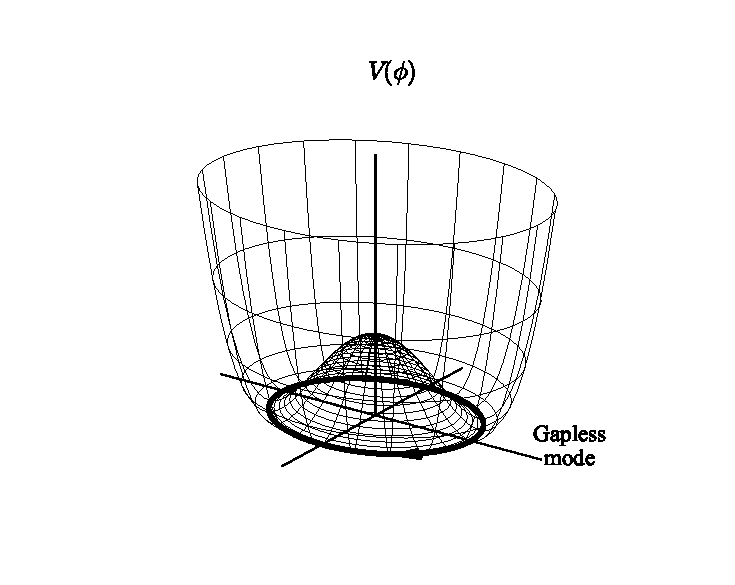
\includegraphics[width=0.72\textwidth]{fig_3.7.pdf}
\caption*{图 3.7\quad 无能隙的 Nambu–Goldstone 模是简并基态之间的涨落。}
\end{figure}

超流相自发破缺 $U(1)$ 对称性：拉格朗日量具有 $U(1)$ 对称性，而基态没有（见 3.3.2 节）。只有在这种情形下，无能隙的声子激发才存在。

Nambu 和 Goldstone 证明了一条普遍定理：如果一个连续对称性在一个相中被\emph{自发}破缺，那么该相必定包含无能隙激发（Nambu, 1960; Goldstone, 1961）。这些无能隙激发通常称为 Nambu–Goldstone 模。超流体中的无能隙声子就是一个 Nambu–Goldstone 模。

直观地说，如果一个对称性（连续的或分立的）被自发破缺，那么各基态必定是简并的，因为哈密顿量具有该对称性而基态没有。不同的基态由对称变换相互联系。此外，\emph{连续}对称性的破缺导致一个简并基态流形，它可以由\emph{连续}变量 $\theta_i$ 参数化。这些简并基态之间的涨落对应于无能隙激发（见图 3.7）。我们可以用 $\theta_i(\pmb{x},t)$ 场写出一个低能有效作用量，来描述无能隙模式的动力学。这个低能有效理论称为非线性 $\sigma$ 模型（nonlinear $\sigma$-model）。XY 模型是最简单的非线性 $\sigma$ 模型。后面我们会看到非线性 $\sigma$ 模型的更多例子。

\subsection{理解有限系统中的自发对称性破缺}

\begin{keypoints}
\item 量子涨落可以恢复对称性。有限系统的真实基态永远不可能破坏 $U(1)$ 对称性。然而，对于大系统，可以用许多近简并的基态构造出一个近似的对称性破缺基态。
\item 对于无限系统，由序参量 $\varphi_0\mathrm{e}^{\mathrm{i}\theta}$ 表征的态自成一个“宇宙”。它要涨落到另一个由不同序参量表征的态，需要无穷长的时间。
\end{keypoints}

% ------------------------------------------------------------
% 块边界备注：
%   起点：书页 78（ch3_a）末行止于 "The energy density (or, more precisely, the"，
%   本块正文以 %JOIN% 续书页 79 顶部半句 "density of the thermal potential) of
%   the classical ground state is"（译作"热势的密度）为"），ch3_a 应将
%   "经典基态的能量密度（或者更精确地说，"写入其 %--A-TAIL-- 区。
%   终点：书页 89（p104）以 3.3.7 节小标题下的要点框自然收尾；书页 90（p105）
%   顶部为新段落 "In Section 3.3.2, we mentioned ..."（式 (3.3.19) 起），
%   无跨页半句，故本块不需要 %--B-TAIL--，ch3_c 直接从书页 90 的新段开始。
%   本块内无 \section 级标题：3.3 节及 3.3.1、3.3.2 小节均在 ch3_a 范围
%   （书页 77–78）；本块起于 3.3.2 节中段，含 \subsection 3.3.3–3.3.7 与
%   问题 3.3.1–3.3.3。
% ------------------------------------------------------------
% 新增术语（ch3_b，待并入术语表"新增术语"区）：
%   superfluid transition 超流相变；
%   first-order / second-order phase transition 一级 / 二级相变；
%   non-analytic point 非解析点；kink 拐折；
%   degenerate ground states 简并基态；manifold 流形；
%   Gibbs energy 吉布斯能；water–vapor transition 水–水蒸气相变；
%   critical point 临界点；critical temperature 临界温度；
%   integrating out (a field) 积掉（某个场）；
%   total derivative / total time derivative 全导数 / 全时间导数；
%   wave equation 波动方程；dispersion 色散；
%   compressibility 压缩率；conductivity 电导率；
%   density–current fluctuations 密度–流涨落；conservation law 守恒定律；
%   particle–wave duality 波粒二象性；quasiparticle 准粒子（已入表）；
%   phonon 声子；roton 旋子；phonon charge 声子电荷；
%   vortex ring 涡环；vortex line 涡线；source / drain 源 / 汇；
%   multipole expansion 多极展开；dipolar interaction 偶极相互作用；
%   canonical momentum 正则动量；canonical commutation relation 正则对易关系；
%   lowering / raising operator 下降 / 上升算符；
%   decoupled harmonic oscillators 退耦谐振子；collective motion 集体运动；
%   toy universe 玩具宇宙；elementary particle 基本粒子；
%   relativistic particle 相对论性粒子；
%   universal properties 普适性质；explicit symmetry breaking 显式（对称性）破缺；
%   Nambu–Goldstone mode Nambu–Goldstone 模
% ------------------------------------------------------------

% 边界备注：起点——书页 90 顶部为完整新段（书页 89 止于 3.3.7 节要点列表），
% 无接缝标记（JOIN）、无上一块收尾（TAIL）可写入；
% 终点——书页 100 止于完整段落（"……描写了超流转变。"），书页 101 顶起新段
% "In the superfluid phase, ..."，本块自然收束，无 TAIL。

在 3.3.2 节中我们提到，超流相（或对称性破缺相）由非零序参量 $\varphi_0$ 表征。在量子理论中，序参量是玻色子场在基态上的期待值 $\varphi_0=\langle\Phi_0|\varphi(\pmb{x})|\Phi_0\rangle=\langle\Phi_0|a(\pmb{x})|\Phi_0\rangle$（记住我们已把玻色子湮灭算符 $a(\pmb{x})$ 改记为 $\varphi(\pmb{x})$）。对于一个有限的量子系统，序参量恒为零，不存在自发对称性破缺。这是因为在量子层次上，$U(1)$ 对称性由算符 $W=\mathrm{e}^{-\mathrm{i}\hat{N}\theta}$ 生成，其中 $\hat{N}$ 是总玻色子数算符。容易验证
\begin{equation*}
Wa(x)W^{\dagger}=\mathrm{e}^{\mathrm{i}\theta}a(x) \tag{3.3.19}
\end{equation*}
由于 $[H,W]=0$，有限系统的基态 $|\Phi_0\rangle$ 总是 $W$ 的本征态。于是 $\langle\Phi_0|a(\pmb{x})|\Phi_0\rangle=\langle\Phi_0|Wa(\pmb{x})W^{\dagger}|\Phi_0\rangle$，因而序参量 $\langle\Phi_0|a(\pmb{x})|\Phi_0\rangle=\langle\Phi_0|\varphi(\pmb{x})|\Phi_0\rangle=0$，无论 $\mu$ 取何值。

与之相对，3.3.2 节中的经典计算确实预言了相变和破缺 $U(1)$ 对称性的简并基态，即使对有限系统也是如此。（事实上，上一节的所有计算都是对体积为 $V$ 的有限系统进行的。）$U(1)$ 对称性之所以能在有限的经典系统中破缺，是因为 $\varphi$ 场的均匀部分 $\varphi_0$ 没有涨落。下面我们将看到，如果把 $\varphi_0$ 当作量子变量处理，它的量子涨落将恢复有限系统的 $U(1)$ 对称性。我们还将看到，当系统体积 $\mathcal{V}\to\infty$ 时，$\varphi_0$ 的量子涨落趋于零。因此，$U(1)$ 对称性破缺可以在量子系统的 $\mathcal{V}\to\infty$ 极限下演生。

我们知道，低能物理由 XY 模型支配。这里我们只关心均匀涨落，于是在式 (3.3.10) 中取 $\theta(\pmb{x},t)=\theta_0(t)$。支配 $\theta_0$ 动力学的有效理论由下式给出
\begin{equation*}
L=\mathcal{V}\big[\frac{1}{2V_0}(\partial_t\theta_0)^2-\rho_0\partial_t\theta_0+\mu\rho_0-\frac{1}{2}V_0\rho_0^2\big] \tag{3.3.20}
\end{equation*}
其中我们放回了一个全时间导数项和一些常数项。式 (3.3.20) 描写一个简单的系统：一个在由 $\theta_0\in[0,2\pi]$ 参数化的圆上运动的粒子。粒子的质量为 $M=\mathcal{V}/V_0$，动量为
\begin{equation*}
p=\partial_{\dot{\theta}_0}L=M\dot{\theta}_0-\frac{\mu\mathcal{V}}{V_0} \tag{3.3.21}
\end{equation*}
其中用到了 $\mu=\rho_0V_0$。哈密顿量为
\begin{equation*}
H=p\dot{\theta}_0-L=\frac{p^2}{2M}+\frac{\mu\mathcal{V}p}{V_0}
\end{equation*}

如果把 $H$ 当作经典系统处理，那么当粒子具有动量 $p=-\mu\mathcal{V}/V_0$（译注：原文为 $-\mu\mathcal{V}p/V_0$，疑多排了一个 $p$），即速度 $\dot{\theta}=0$ 时，它处于基态。粒子的位置可以任意。因此，描写粒子处于不同 $\theta_0$ 的所有态 $|\theta_0\rangle$ 都是简并的基态，$U(1)$ 对称性破缺。

然而，量子理论给出了一幅截然不同的图像。在量子理论中，动量 $p$ 按整数量子化。动量为 $p=-n$ 的态具有能量
\begin{equation*}
E_n=\frac{n^2}{2M}-\frac{\mu\mathcal{V}n}{V_0M}=\frac{V_0n^2}{2\mathcal{V}}-\mu n \tag{3.3.22}
\end{equation*}
因此，$-p=n=\mu\mathcal{V}/V_0$ 的态能量最小，对应于真正的基态
\begin{equation*}
|\Phi_0\rangle=\int\mathrm{d}\theta_0\,\mathrm{e}^{-\mathrm{i}\frac{\mu\mathcal{V}}{V_0}\theta_0}|\theta_0\rangle
\end{equation*}
基态没有简并。现在可以明确地证明序参量为零：
\begin{equation*}
\langle\Phi_0|\varphi_0\mathrm{e}^{\mathrm{i}\theta_0}|\Phi_0\rangle=0
\end{equation*}

理解为什么没有 $U(1)$ 对称性破缺的另一种方式，是注意到总玻色子数为 $N=\mathcal{V}(\rho_0-\frac{\partial_t\theta_0}{V_0})$（见式 (3.3.13)）。由式 (3.3.21) 可见，$-N=p$ 正是 $\theta_0$ 的正则动量（canonical momentum）。因此，在量子世界中二者之间存在不确定关系（uncertainty relation）：
\begin{equation*}
[\hat{N},\theta_0]=\mathrm{i},\qquad \Delta N\,\Delta\theta_0\sim 1/2
\end{equation*}
所以，粒子数固定的有限系统不可能具有确定的相位 $\theta_0$。要得到对称性破缺态，我们必须允许粒子数容易地涨落。\footnote{因此，如果添加或移走一个玻色子需要花费有限的能量，那么该系统就不可能处于 $U(1)$ 对称性破缺相。作为这一理解的一个应用，让我们考虑一个具有强在位排斥（on-site repulsion）的格点玻色子系统 $H=\sum_{\langle ij\rangle}t_{ij}a_i^{\dagger}a_j+\sum_r U(a_r^{\dagger}a_r)^2$，其中 $U\gg t_{ij}$。若玻色子密度恰好是每格点整数个玻色子，则该系统不可能处于超流相，因为在这个密度下添加或移走一个玻色子需要花费有限的能量。}

虽然量子涨落消除了简并、恢复了有限系统的 $U(1)$ 对称性，但对于大系统，低激发态是近乎简并的。能隙只有 $V_0/\mathcal{V}$ 的量级，当 $\mathcal{V}\to\infty$ 时趋于 0。如果该能隙低于所有我们感兴趣的能标（例如低于测量的能量分辨率），那么在一切实际用途中，这些低激发态都可以认为是简并的。这时，有限系统可以认为具有 $U(1)$ 对称性破缺。在问题 3.3.4 中我们将看到，如果我们制备一个相位为 $\theta_0$ 的态，那么当系统很大时，相位要经过很长时间才能变到其他值。因此，在短的时间间隔内，我们可以把相位当作刻画对称性破缺基态的一个常数。

在 3.3.2 节的末尾我们讨论过序参量和长程关联。本节讨论一类特殊的量子涨落——$\varphi$ 的均匀相位涨落。我们看到，对于有限系统，即使 $\mu>0$，这类涨落也会破坏序参量。但同样清楚的是，$\mu>0$ 时存在的长程关联不会被均匀相位涨落破坏。因此，对于大的有限系统，我们可以用长程关联来刻画对称性破缺相变。

在上面的讨论中，我们只考虑了 $\theta$ 的均匀涨落，忽略了依赖空间的涨落。这里的问题是，什么时候这样做才是正确的？我们注意到，依赖空间的涨落对应于具有有限动量的声波。这些声波激发的最小能隙为 $2\pi v/L$，其中 $L$ 是系统的线度。于是，在能量 $2\pi v/L$ 以下，我们可以忽略依赖空间的 $\theta$ 涨落，只考虑均匀涨落。本节的讨论仅在 $2\pi v/L$ 以下有效。

具有固定角度的对称性破缺态 $|\theta_0\rangle$ 由 $|\theta_0\rangle=\sum_n\mathrm{e}^{\mathrm{i}\theta_0 n}|n\rangle$ 给出。要在上述近似之内构造这样一个态，我们需要在能量 $2\pi v/L$ 以下容纳无穷多个均匀涨落。在一维以外，均匀涨落的能隙为 $V_0/\mathcal{V}$，远小于声波的能隙。在 $L\to\infty$ 极限下，$2\pi v/L$ 以下有无穷多条均匀涨落的能级。因此，在一维以外可以构造对称性破缺态。在一维，$2\pi v/L$ 以下的均匀态数目有限，我们难以构造出对称性破缺态。在 3.3.8 节中我们将看到，一维的超流相不可能具有真正的长程序。

\subsection*{问题 3.3.4}

考虑零温下 $1\,\mathrm{cm}^3$ 的超流 $\mathrm{He}_4$。我们制备一个相位 $\langle\theta_0\rangle=0$ 的“基态”。假设相位的弥散为 $\sqrt{\langle\theta_0^2\rangle}=\pi/10$。问经过多长时间相位的弥散会达到 $2\pi$，使得基态的相位不再能定义？（提示：你需要猜测 $\mathrm{He}_4$ 中声波速度的数量级，以便估计 $V_0$——$V_0$ 恰好是压缩率（compressibility）的倒数。）

\subsection{低维中的超流相}

\begin{keypoints}
\item 与 Nambu--Goldstone 模相联系的量子涨落可以破坏低维中的长程序和超流相。
\item 量子涨落对量子临界点（quantum critical point）的影响，以及上临界维数（upper critical dimension）的概念。
\end{keypoints}

在 3.3.2 节的末尾，我们证明了对称性破缺相中长程序的存在。然而，那个计算几乎是在作弊，因为只考虑经典基态，就不允许存在依赖空间的相位涨落，其结果是不同位置处的相位总是关联的。这里我们将研究依赖空间的相位涨落的效应，看看长程关联何时能在依赖空间的相位涨落下存活。

首先考虑零温下的玻色子系统。我们想计算 $\langle\varphi^{\dagger}(t,\pmb{x})\varphi(0,0)\rangle$。由于只关心低能激发，我们将使用有效 XY 模型（式 (3.3.10)），它可以改写为
\begin{equation*}
L=\frac{\chi}{2}\big((\partial_t\theta)^2-v^2(\partial_{\pmb{x}}\theta)^2\big) \tag{3.3.23}
\end{equation*}
其中 $\chi=1/V_0$ 是超流的压缩率。在路径积分方法中，关联函数可以写为
\begin{equation*}
\big\langle\varphi(t,\pmb{x})^{\dagger}\varphi(0,0)\big\rangle=|\varphi_0|^2\big\langle\mathrm{e}^{-\mathrm{i}\theta(t,\pmb{x})}\mathrm{e}^{\mathrm{i}\theta(0,0)}\big\rangle=\frac{\int\mathcal{D}\theta\,\mathrm{e}^{-\mathrm{i}\theta(t,\pmb{x})}\mathrm{e}^{\mathrm{i}\theta(0,0)}\mathrm{e}^{\mathrm{i}S}}{\int\mathcal{D}\theta\,\mathrm{e}^{\mathrm{i}S}}
\end{equation*}
引入
\begin{equation*}
Z[f(t,\pmb{x})]=\int\mathcal{D}\theta\,\mathrm{e}^{\mathrm{i}S}\mathrm{e}^{\mathrm{i}\int\mathrm{d}t\,\mathrm{d}^d\pmb{x}\,f(t,\pmb{x})\theta(t,\pmb{x})}
\end{equation*}
我们看到
\begin{equation*}
\big\langle\mathrm{e}^{-\mathrm{i}\theta(t_0,\pmb{x}_0)}\mathrm{e}^{\mathrm{i}\theta(0,0)}\big\rangle=\frac{Z[-\delta(t-t_0,\pmb{x}-\pmb{x}_0)+\delta(t,\pmb{x})]}{Z[0]}
\end{equation*}
这里 $Z[f(t,\pmb{x})]/Z[0]$ 可以用高斯积分容易地算出：
\begin{equation*}
\frac{Z[f(t,\pmb{x})]}{Z[0]}=\mathrm{e}^{-\mathrm{i}\frac{1}{2}\int\mathrm{d}t_1\mathrm{d}\pmb{x}_1\mathrm{d}t_2\mathrm{d}\pmb{x}_2\,f(t_1,\pmb{x}_1)G_{\theta}(t_1-t_2,\pmb{x}_1-\pmb{x}_2)f(t_2,\pmb{x}_2)}
\end{equation*}
其中 $G_{\theta}$ 是 $\chi(-\partial_t^2+v^2\partial_{\pmb{x}}^2)$ 的逆。它也是 $\theta$ 场的关联函数：
\begin{equation*}
\mathrm{i}G_{\theta}(t,\pmb{x})=\langle T[\theta(t,\pmb{x})\theta(0,0)]\rangle
\end{equation*}
我们发现
\begin{equation*}
\big\langle\mathrm{e}^{-\mathrm{i}\theta(t,\pmb{x})}\mathrm{e}^{\mathrm{i}\theta(0,0)}\big\rangle=\mathrm{e}^{\mathrm{i}G_{\theta}(t,\pmb{x})}\mathrm{e}^{-\mathrm{i}G_{\theta}(0,0)}\propto\mathrm{e}^{\langle(-\mathrm{i}\theta(t,\pmb{x}))(\mathrm{i}\theta(0,0))\rangle}
\end{equation*}

\subsubsection{$1+1$ 维中的超流相}

$k$--$\omega$ 空间中的关联函数由下式给出
\begin{equation*}
G_{\theta}(\omega,\pmb{k})=\frac{\chi^{-1}}{\omega^2-v^2\pmb{k}^2+\mathrm{i}0^+}.
\end{equation*}
我们可以用它按如下方式计算 $1+1$ 维的 $G_{\theta}(t,\pmb{x})$：
\begin{align*}
G_{\theta}(t,x)&=\int\frac{\mathrm{d}k\,\mathrm{d}\omega}{(2\pi)^2}\,G_{\theta}(\omega,k)\,\mathrm{e}^{\mathrm{i}(-\omega t+kx)}\\
&=\chi^{-1}\int\frac{\mathrm{d}k\,\mathrm{d}\omega}{(2\pi)^2}\,\frac{1}{2v|k|}\left(\frac{1}{\omega-v|k|+\mathrm{i}0^+}-\frac{1}{\omega+v|k|-\mathrm{i}0^+}\right)\mathrm{e}^{\mathrm{i}(\omega t-kx)}\\
&=\left\{\begin{array}{ll}
\chi^{-1}\displaystyle\int\frac{\mathrm{d}k}{(2\pi)^2}\,\frac{-\mathrm{i}\pi}{v|k|}\,\mathrm{e}^{\mathrm{i}(-v|k|t+kx)}, & t>0\\[10pt]
\chi^{-1}\displaystyle\int\frac{\mathrm{d}k}{(2\pi)^2}\,\frac{-\mathrm{i}\pi}{v|k|}\,\mathrm{e}^{\mathrm{i}(+v|k|t+kx)}, & t<0
\end{array}\right.\\
&=\chi^{-1}\int\frac{\mathrm{d}k}{(2\pi)^2}\,\frac{-\mathrm{i}\pi}{v|k|}\,\mathrm{e}^{\mathrm{i}(-v|k||t|+kx)}
\end{align*}
对于有限系统，$k$ 是量子化的：$k=\frac{2\pi}{L}\times\text{整数}$。把 $\int\mathrm{d}k/2\pi$ 换成 $L^{-1}\sum_k$ 后，我们得到
\begin{align*}
G_{\theta}(t,x)&=\chi^{-1}L^{-1}\sum_k\frac{-\mathrm{i}}{2v|k|}\,\mathrm{e}^{\mathrm{i}(-v|k||t|+kx)}\\
&=\frac{\mathrm{i}}{4\pi v\chi}\left(\ln\big(1-\mathrm{e}^{2\pi\mathrm{i}\frac{-v|t|+x}{L}-0^+}\big)+\ln\big(1-\mathrm{e}^{2\pi\mathrm{i}\frac{-v|t|-x}{L}-0^+}\big)\right)
\end{align*}
两个对数项分别来自 $k>0$ 与 $k<0$ 的求和。$k=0$ 项是常数，已被略去。如果 $v|t|,\,x\ll L$，则
\begin{equation*}
G_{\theta}(t,x)=\frac{\mathrm{i}}{4\pi v\chi}\ln 4\pi^2\frac{x^2-v^2t^2+\mathrm{i}0^+}{L^2} \tag{3.3.24}
\end{equation*}
我们看到，在 $1+1$ 维中，
\begin{align*}
\big\langle\mathrm{e}^{-\mathrm{i}\theta(t,x)}\mathrm{e}^{\mathrm{i}\theta(0,0)}\big\rangle&=\mathrm{e}^{-\mathrm{i}G_{\theta}(0,0)}\left(\frac{L^2}{4\pi^2(x^2-v^2t^2+\mathrm{i}0^+)}\right)^{1/4\pi v\chi}\\
&=\mathrm{e}^{-\mathrm{i}G_{\theta}(0,0)}\,\mathrm{e}^{-\mathrm{i}\frac{\pi}{4\pi v\chi}\Theta(v^2t^2-x^2)}\left(\frac{L^2}{4\pi^2|x^2-v^2t^2|}\right)^{1/4\pi v\chi}
\end{align*}
由式 (3.3.24)，$G_{\theta}(0,0)=-\mathrm{i}\infty$，这似乎意味着 $\langle\mathrm{e}^{-\mathrm{i}\theta(t,x)}\mathrm{e}^{\mathrm{i}\theta(0,0)}\rangle=0$。我们提醒，XY 模型只是一个低能有效理论，它在短距离处失效。$G_{\theta}(0,0)$ 的发散应当被一个短距离标度 $l$ 截断。于是，我们可以把 $G_{\theta}(0,0)$ 换成 $G_{\theta}(0,l)$，这就得到
\begin{align*}
\big\langle\mathrm{e}^{-\mathrm{i}\theta(t,x)}\mathrm{e}^{\mathrm{i}\theta(0,0)}\big\rangle&=\left(\frac{l^2}{x^2-v^2t^2+\mathrm{i}0^+}\right)^{1/4\pi v\chi}\\
&=\mathrm{e}^{-\mathrm{i}\frac{\pi}{4\pi v\chi}\Theta(v^2t^2-x^2)}\left(\frac{l^2}{|x^2-v^2t^2|}\right)^{1/4\pi v\chi} \tag{3.3.25}
\end{align*}

上述结果告诉我们，在 $1+1$ 维中量子涨落破坏长程序，不存在对称性破缺。但这种破坏并不彻底。$\varphi$ 场仍然具有“准长程序”（quasi-long-range order），其关联按代数方式衰减。这导致如下相图：无论 $\mu<0$ 还是 $\mu>0$，玻色子基态都不破缺 $U(1)$ 对称性。然而，当 $\mu<0$ 时玻色子场只有短程关联；当 $\mu>0$ 时，短程关联被提升为按代数衰减的“准长程”关联。

另一个重要之点是，关联 $\langle\mathrm{e}^{-\mathrm{i}\theta(t,x)}\mathrm{e}^{\mathrm{i}\theta(0,0)}\rangle$ 无法只用有效理论中的参数来表达，它还依赖一个短距离截断标度 $l$。这并不奇怪。要得到低能 XY 模型，我们必须扔掉原理论在短距离和高能量处的大量信息与结构。许多算符的定义本身就依赖这些短距离结构。例如，有些算符是同一空间点上的场量的乘积，而在低能有效理论中，“同一空间点”这一概念已经丧失，至少变得模糊。因此，我们不应指望把所有关联函数都用有效理论中的参数表达。在上面的例子中，我们发现关联 $\langle\mathrm{e}^{-\mathrm{i}\theta(t,x)}\mathrm{e}^{\mathrm{i}\theta(0,0)}\rangle$ 确实依赖理论的短距离结构。令人惊讶的是，所有复杂的短距离结构竟被总结进单一参数 $l$ 之中。这展示了低能有效理论的普适性（universality）。

\subsubsection{$2+1$ 维中的超流相}

为计算 $2+1$ 维的 $G_{\theta}$，我们先计算虚时关联
\begin{equation*}
\mathcal{G}_{\theta}(x^i)=\langle\theta(x^i)\theta(0)\rangle
\end{equation*}
这里 $x^{1,2}$ 是空间坐标，$x^3$ 是虚时间。为简单起见，我们取 $v=1$。XY 模型的配分函数为 $Z=\int\mathcal{D}\theta\,\exp(-\int\mathrm{d}^3x^i\,\frac{\chi}{2}(\partial_i\theta)^2)$。我们看到\footnote{我们用到了 $-\partial_i^2\,r^{-1}=4\pi\delta(x^i)$。}
\begin{equation*}
\mathcal{G}_{\theta}(x^i)=\frac{\chi^{-1}}{-\partial_i^2}=\frac{1}{4\pi\chi r}=\frac{1}{4\pi\chi\sqrt{\pmb{x}^2+\tau^2}}
\end{equation*}
其中 $r^2=x^ix^i$。

由 $\mathrm{i}G_{\theta}$ 与 $\mathcal{G}_{\theta}$ 之间的关系（见式 (2.2.34)），我们得到
\begin{equation*}
\mathrm{i}G_{\theta}(t,x^1,x^2)=\mathcal{G}_{\theta}(x^1,x^2,\mathrm{e}^{\mathrm{i}\pi/2}t)=\frac{1}{4\pi\chi}\frac{1}{\sqrt{\pmb{x}^2-t^2}}
\end{equation*}
然而，当 $|t|>|\pmb{x}|$ 时传播子是含糊的：$\mathrm{i}G_{\theta}(t,x^1,x^2)=\pm\mathrm{i}\frac{1}{4\pi\chi}\frac{1}{\sqrt{|\pmb{x}^2-t^2|}}$。要固定 $\pm$ 号，我们需要更仔细地进行解析延拓。假设 $|t|\gg|\pmb{x}|$，并让 $\mathcal{G}_{\theta}(x^1,x^2,\mathrm{e}^{\mathrm{i}\eta}t)$ 中的 $\eta$ 从 0 连续地变到 $\pi/2$，我们发现
\begin{equation*}
\mathrm{i}G_{\theta}(t,x^1,x^2)=\frac{1}{4\pi v\chi}\frac{1}{\sqrt{|\pmb{x}^2-vt^2|}}\,\mathrm{e}^{-\mathrm{i}\frac{\pi}{2}\Theta(v|t|-|\pmb{x}|)}
\end{equation*}
其中我们已恢复速度 $v$。

无论如何，当 $|t|$ 与 $|\pmb{x}|$ 趋于 $\infty$ 时，$\mathrm{i}G(\pmb{x},t)\to 0$。因此，$\langle\mathrm{e}^{-\mathrm{i}\theta(t,x)}\mathrm{e}^{\mathrm{i}\theta(0,0)}\rangle$ 在长距离处趋于常数 $\mathrm{e}^{-\mathrm{i}G_{\theta}(0,0)}$。然而，该常数的数值不同于经典值（经典值为 1）。引入短距离截断标度 $l$，我们看到
\begin{equation*}
\big\langle\mathrm{e}^{-\mathrm{i}\theta(t,x)}\mathrm{e}^{\mathrm{i}\theta(0,0)}\big\rangle\to\mathrm{e}^{-\frac{1}{4\pi v\chi l}}=\big\langle\mathrm{e}^{-\mathrm{i}\theta(t,x)}\big\rangle\big\langle\mathrm{e}^{\mathrm{i}\theta(0,0)}\big\rangle \tag{3.3.26}
\end{equation*}
我们发现，相涨落在 $2+1$ 维及更高维中不破坏长程序，只是减小序参量的数值。

\subsubsection{短距离截断与非线性效应}

在上面，我们讨论了量子涨落对经典基态的影响。我们发现，在 $1+1$ 维中，量子涨落总是有很大的影响——它们破坏长程序。破坏长程序的量子涨落来自长波长和低频率。无论我们如何调整理论中的参数（例如截断标度），它们都在那里。在 $2+1$ 维及更高维中，长波长、低频涨落不产生发散的效应，一般说来长程序能在量子涨落下存活。序参量敏感地依赖截断标度这一事实表明，序参量的减小量由短距离涨落决定。短距离涨落只是在定量上修正经典结果。

现在产生了一个问题：这些定量修正何时很小？也就是说，经典近似何时能定量地描写系统的物理性质？从关于序参量的结果（见式 (3.3.26)）我们看到，如果截断标度 $l\gg(v\chi)^{-1}$，涨落修正就很小。为得到截断标度，注意我们在式 (3.3.9) 中略去了 $\frac{\varphi_0^2}{2m}\partial_{\pmb{x}}^2$ 项，因为我们假定 $\theta$ 的涨落是平滑的。然而，在短距离标度处，当 $\frac{\varphi_0^2}{2m}\partial_{\pmb{x}}^2$ 与另一项 $2V_0\varphi_0^4$ 可比时，我们不能再忽略梯度项，XY 模型失效。这一跨越长度标度（crossover length scale）由
\begin{equation*}
\xi=(4mV_0\varphi_0^2)^{-1/2}
\end{equation*}
给出，称为相干长度（coherence length）。相干长度有如下含义：如果我们改变某一点的 $h$ 场或玻色子密度，那么这种改变将在 $\xi$ 的距离上传播。取 $l=\xi$，约化因子变为
\begin{equation*}
\mathrm{e}^{-\frac{1}{4\pi v\chi l}}=\mathrm{e}^{-\frac{mV_0}{\sqrt{2}\pi}} \tag{3.3.27}
\end{equation*}
我们可以把上述结果改写成一个更有意义的形式。注意 $E_{int}\equiv\frac{1}{2}V_0\varphi_0^2$ 具有能量的量纲，它表示每个粒子的相互作用能。在 $2+1$ 维中，$E_{qua}\equiv\rho_0/m$ 也具有能量的量纲。$E_{qua}$ 是这样一个能标（或温度标度），低于它时玻色子波函数开始交叠，我们需要把玻色子当作量子系统来处理。现在我们可以把约化因子改写为
\begin{equation*}
\mathrm{e}^{-\frac{1}{4\pi v\chi l}}=\mathrm{e}^{-\frac{\sqrt{2}E_{int}}{E_{qua}}}
\end{equation*}
我们看到，在弱相互作用极限下涨落修正很小，经典结果良好。

然而，上述结果并不完整，因为我们只在二次近似之内考虑了短距离涨落的效应，还没有考虑高阶项带来的非线性效应。为了更系统地研究涨落的效应，我们想对我们的玻色子作用量作量纲分析（dimensional analysis）：
\begin{equation*}
S=\int\mathrm{d}^d\pmb{x}\,\mathrm{d}t\,\Big[\mathrm{i}\frac{1}{2}\big(\varphi^*\partial_t\varphi-\varphi\partial_t\varphi^*\big)-\frac{1}{2m}\partial_{\pmb{x}}\varphi^*\partial_{\pmb{x}}\varphi-\frac{V_0}{2}|\varphi|^2\big(|\varphi|^2-2\rho_0\big)\Big] \tag{3.3.28}
\end{equation*}
这里我们取了 $\mu=V_0\rho_0$。我们想重新标度 $t$、$\pmb{x}$ 和 $\varphi$，把作用量改写成 $S=\tilde{S}/g$ 的形式，使得 $\tilde{S}$ 中所有的系数都是 1 的量级。我们发现下述重新标度即可奏效：
\begin{equation*}
x=\xi\tilde{x},\qquad t=(V_0\rho_0)^{-1}\tilde{t},\qquad\varphi=\sqrt{\rho_0}\,\tilde{\varphi}
\end{equation*}
它给出
\begin{equation*}
S=g^{-1}\int\mathrm{d}^d\tilde{\pmb{x}}\,\mathrm{d}\tilde{t}\,\Big[\mathrm{i}\frac{1}{2}\big(\tilde{\varphi}^*\partial_t\tilde{\varphi}-\tilde{\varphi}\partial_t\tilde{\varphi}^*\big)-2\partial_{\pmb{x}}\tilde{\varphi}^*\partial_{\pmb{x}}\tilde{\varphi}-\frac{1}{2}|\tilde{\varphi}|^2\big(|\tilde{\varphi}|^2-2\big)\Big]
\end{equation*}
其中
\begin{equation*}
g=N_{\xi}^{-1},\qquad N_{\xi}=\rho_0\xi^d
\end{equation*}
这里 $N_{\xi}$ 是体积 $\xi^d$ 中的粒子数。我们也可以把 $g$ 写成
\begin{equation*}
g=\sqrt{\rho_0^{d-2}(4mV_0)^d} \tag{3.3.29}
\end{equation*}

现在很清楚，如果路径积分 $\int\mathcal{D}^2\tilde{\varphi}\,\mathrm{e}^{\mathrm{i}\frac{\tilde{S}}{g}}$ 中的 $g$ 很小，那么“势”很陡，势能极小值附近的涨落很小。这时，半经典近似（semiclassical approximation）是好的。实际上，半经典近似正对应于按 $g$ 的展开。在 $2+1$ 维中 $g=4mV_0$，它恰好与从短距离涨落得到的条件 (3.3.27) 相符。

当 $g$ 大时，涨落可以大到这样的程度，以至于经典图像在定性上是否正确都不清楚了。事实上，人们相信，当 $g\gg1$ 时，短距离涨落可以破坏长程序并在基态中恢复 $U(1)$ 对称性，例如通过形成晶体（晶体具有不同的对称性破缺和不同的长程序）。这与 $1+1$ 维的情形形成对照，在那里无论 $g$ 取何值，长距离涨落都破坏长程序。

按照经典理论，我们的玻色子系统在 $\mu=0$ 处经历一个量子相变（quantum phase transition）。该相变是连续的，由一个量子临界点描写。在经典理论之内，我们可以计算出所有的临界指数。例如，$\omega\propto k^z$ 中的动力学指数（dynamical exponent）$z$ 为 $z=2$；$\langle\varphi\rangle=\varphi_0\propto\mu^{\nu}$ 中的指数 $\nu$ 为 $\nu=1/2$。问题是，经典理论能正确地描写量子临界点吗？由式 (3.3.29) 可见，如果 $d>2$，那么我们离临界点（$\rho_0\to0$）越近，$g$ 越小，半经典近似就越好。因此，对于 $d>2$，经典理论能正确地描写量子临界点。然而，对于 $d<2$，当我们逼近临界点时 $g$ 发散。在这种情况下，我们必须把量子涨落包括进来才能得到正确的临界指数。这一跨越空间维数 $d_c=2$ 称为该临界点的上临界维数。

\subsection*{问题 3.3.5}

考虑一个具有长程相互作用的玻色子系统
\begin{equation*}
\frac{1}{2}\int\mathrm{d}^d\pmb{x}\,\mathrm{d}^d\pmb{x}'\,|\varphi(\pmb{x})|^2V(\pmb{x}-\pmb{x}')|\varphi(\pmb{x}')|^2
\end{equation*}
其中 $V(r)=V_dr^{\epsilon-d}$。如果 $\epsilon<0$，则相互作用实际上是短程的。这里我们假设 $\epsilon>0$。
\begin{enumerate}
\item 推导修改后的 XY 模型。
\item 找出临界空间维数 $d_l$，低于它时相位涨落 $\theta$ 总是破坏长程序。这里我们把维数当作连续的实数处理。我们知道，对于短程相互作用 $d_l=1$。
\item 重复本节末尾的讨论，求出 $g$（它决定量子涨落何时很小）以及上临界维数 $d_c$（超过它时经典理论能正确描写量子临界点）。
\end{enumerate}

\subsection*{问题 3.3.6}

$1+1$ 维中的有限温关联。
\begin{enumerate}
\item 计算虚时关联
\begin{equation*}
\mathcal{G}(x,\tau)=\big\langle\mathrm{e}^{\mathrm{i}\theta(x,\tau)}\mathrm{e}^{-\mathrm{i}\theta(0,0)}\big\rangle
\end{equation*}
假设一维空间是长度为 $L$ 的有限圆。
\item 计算有限温下的虚时关联 $\mathcal{G}^{\beta}(x,\tau)$，假设一维空间是一条无限长的直线。（提示：你可以交换 $x$ 与 $\tau$，并利用第 1 问的结果。）
\item 计算有限温下的实时（编时）关联 $G^{\beta}(x,t)$，假设一维空间是一条无限长的直线。证明
\begin{equation*}
G^{\beta}(0,t)\propto\mathrm{e}^{-\mathrm{i}\frac{\pi}{4\pi v\chi}}\left(\frac{\pi T}{\sinh(\pi T|t|)}\right)^{1/2\pi v\chi}
\end{equation*}
\end{enumerate}

\section{有限温度下的超流相}

\subsection{有限温度下的路径积分}

\begin{keypoints}
\item $(d+1)$ 维量子系统在有限温度下的长距离性质，可以用一个 $d$ 维系统的路径积分来描写。
\end{keypoints}

本节中，我们将研究一个相互作用玻色子系统及其有限温度下的超流相。我们从虚时路径积分
\begin{equation*}
Z=\int\mathcal{D}^2[\varphi(\pmb{x},\tau)]\,\mathrm{e}^{-\int_0^{\beta}\mathrm{d}^d\pmb{x}\,\mathrm{d}\tau\,\big[\frac{1}{2}(\varphi^*\partial_{\tau}\varphi-\varphi\partial_{\tau}\varphi^*)+\frac{1}{2m}\partial_{\pmb{x}}\varphi^*\partial_{\pmb{x}}\varphi-\mu|\varphi|^2+\frac{V_0}{2}|\varphi|^4\big]}
\end{equation*}
出发，它表示系统的配分函数。注意，贝里相项在虚时路径积分中保持为虚的。

为了把上述配分函数约化为一个熟悉的统计模型，我们先通过引入
\begin{equation*}
\varphi_{\omega_n}(\pmb{x})=\beta^{-1}\int_0^{\beta}\mathrm{d}\tau\,\varphi(\pmb{x},\tau)\mathrm{e}^{\mathrm{i}\tau\omega_n}
\end{equation*}
进入离散频率空间。然后，我们积掉所有有限频率的模式：
\begin{equation*}
Z=\int\prod_n\mathcal{D}^2[\varphi_{\omega_n}]\,\mathrm{e}^{-S}=\int\mathcal{D}^2[\varphi_c(\pmb{x})]\,\mathrm{e}^{-S_{\mathrm{eff}}}
\end{equation*}
其中 $\varphi_c(\pmb{x})=\varphi_{\omega_n=0}(\pmb{x})$ 是零频率模式。这一步很困难，所得的有效作用量 $S_{\mathrm{eff}}$ 可以非常复杂，甚至可以包含非局域项，例如 $\int\mathrm{d}^d\pmb{x}\,\mathrm{d}^d\pmb{x}'\,|\varphi_c(\pmb{x})|^2K(\pmb{x}-\pmb{x}')|\varphi_c(\pmb{x}')|^2$。然而，在有限频率处，原作用量包含 $\mathrm{i}|\varphi_c(\pmb{x})|^2\omega_n$ 项，它使 $\varphi_n$ 的传播子具有 $1/(\mathrm{i}\omega_n+ck^2+\mu)$ 的形式。该传播子是短程的，按指数衰减。因此，非零模式的涨落只能传递短程相互作用，$K(\pmb{x}-\pmb{x}')$ 应具有指数衰减：$K(\pmb{x}-\pmb{x}')\sim\mathrm{e}^{-|\pmb{x}-\pmb{x}'|/l_T}$。这里我们有一个新的长度标度 $l_T$，超出它之后，有效作用量 $S_{\mathrm{eff}}$ 就可以当作局域作用量处理。尽管 $S_{\mathrm{eff}}$ 可以非常复杂，但由于其对称性，局域作用量只能取某种确定的形式。在超出 $l_T$ 的长距离处，我们可以作梯度展开（gradient expansion）
\begin{equation*}
S_{\mathrm{eff}}=\beta\int\mathrm{d}^dx\,\big[\frac{1}{2m^*}|\partial_x\varphi_c|^2+V(|\varphi_c|,T)+\dots\big] \tag{3.4.1}
\end{equation*}
“…”代表更高阶导数项。有效势（effective potential）依赖于温度。当 $\mu<0$ 时，我们预期 $V$ 总有一个位于 $\varphi_c=0$ 的单一极小，代表对称态。当 $\mu>0$ 且温度较低时，$V$ 应有一个位于 $\varphi_c=\varphi_0\mathrm{e}^{\mathrm{i}\theta}$ 的极小圆圈，代表对称性破缺态。然而，超出临界温度 $T_c$ 之后，预期 $V$ 会变成在 $\varphi_c=0$ 处只有一个单一极小的形式。因此，$V$ 对温度的依赖描写了超流转变。

% ==================================================================
% 新增术语（ch3_c 新增，供术语表追加）：
%   canonical momentum 正则动量；uncertainty relation 不确定关系；
%   on-site repulsion 在位排斥；lattice boson system 格点玻色子系统；
%   compressibility 压缩率；Nambu–Goldstone modes Nambu–Goldstone 模；
%   quasi-long-range order 准长程序；universality 普适性；
%   short-distance cut-off (scale) 短距离截断（标度）；crossover length scale 跨越长度标度；
%   coherence length 相干长度；interaction energy per particle 每粒子相互作用能；
%   dimensional analysis 量纲分析；semiclassical approximation 半经典近似；
%   quantum phase transition 量子相变；quantum critical point 量子临界点；
%   dynamical exponent 动力学指数；upper critical dimension 上临界维数；
%   quantum critical exponents 量子临界指数；long-range interaction 长程相互作用；
%   zero-frequency mode 零频率模式；discrete frequency space 离散频率空间；
%   non-local term 非局域项；gradient expansion 梯度展开；
%   effective potential 有效势；phase fluctuation 相位涨落
% ==================================================================

其中 $K(\pmb{x}) = n^{2}\langle \delta\theta(\pmb{x})\delta\theta(0)\rangle$。我们注意到，最后一项可以改写为

% ---- 书页 101 (p116) ----
在超流相中，只有相位涨落在长距离下才是重要的。令 $\varphi_c(\pmb{x}) = \varphi_0\mathrm{e}^{\mathrm{i}\theta(\pmb{x})}$，我们便得到一个 XY 模型
\begin{equation*}
S_{\mathrm{eff}} = \int \mathrm{d}^{d}\pmb{x}\ \frac{\eta}{2}(\partial_{\pmb{x}}\theta)^{2}
\tag{3.4.2}
\end{equation*}
其中
\begin{equation*}
\eta = \frac{\varphi_{0}^{2}}{mT}
\tag{3.4.3}
\end{equation*}
我们注意到，能量由 $TS_{\mathrm{eff}}$ 给出。因此，$T\eta$ 的数值决定了相位扭转 $\partial_{\pmb{x}}\theta \neq 0$ 的能量代价。这里 $T\eta$ 称为 XY 模型的相位劲度（phase rigidity）。

当然，以上关于对称性破缺的讨论都基于经典图像，其中我们忽略了 $\varphi$ 和 $\theta$ 的涨落。（现在这些涨落对应于热涨落。）我们同样可以问：对称性破缺态能否在热涨落下存活？与上一节一样，我们可以用 XY 模型来处理这个问题。利用那些结果，我们发现，对于 $d>2$，热涨落并不总是破坏长程序。

对于 $d<2$，热涨落总是破坏长程序，把它变为短程序。这是因为，对于 $d<2$，$\theta$ 的关联随 $|\pmb{x}|$ 呈幂次发散：
\begin{equation*}
\begin{aligned}
&\ \langle \theta(\pmb{x})\theta(0)\rangle - \langle \theta(l)\theta(0)\rangle
 = C_{d}\eta^{-1}(L^{2-d} - |\pmb{x}|^{2-d}) - C_{d}\eta^{-1}(L^{2-d} - l^{2-d}) \\
&\ = -C_{d}\eta^{-1}|\pmb{x}|^{2-d}
\end{aligned}
\end{equation*}
这里用到了傅里叶变换
\begin{equation*}
\int \mathrm{d}^{d}\pmb{k}\ \frac{\mathrm{e}^{\mathrm{i}\pmb{k}\cdot\pmb{x}}}{\eta|\pmb{k}|^{2}} = C_{d}\eta^{-1}(L^{2-d} - |\pmb{x}|^{2-d})
\end{equation*}
因此，
\begin{equation*}
\left\langle \mathrm{e}^{\mathrm{i}n\theta(\pmb{x})}\mathrm{e}^{-\mathrm{i}n\theta(0)} \right\rangle
= \mathrm{e}^{-\frac{n^{2}}{2}\langle \theta(\pmb{x})-\theta(0)\rangle^{2}}
= \mathrm{e}^{n^{2}\langle \theta(\pmb{x})\theta(0)\rangle - n^{2}\langle \theta(l)\theta(0)\rangle}
= \mathrm{e}^{-C_{d}n^{2}\eta^{-1}|\pmb{x}|^{2-d}}
\end{equation*}
当 $n=1$ 时，衰减长度为 $(\eta/C_{d})^{1/(2-d)}$。

对于 $d=2$，$\theta$ 关联具有对数发散 $\langle \theta(\pmb{x})\theta(0)\rangle - \langle \theta(l)\theta(0)\rangle = -\frac{1}{2\pi\eta}\ln(|\pmb{x}|/l)$，我们有以下的代数长程序（algebraic long-range order）：
\begin{equation*}
\left\langle \mathrm{e}^{\mathrm{i}n\theta(\pmb{x})}\mathrm{e}^{-\mathrm{i}n\theta(0)} \right\rangle \sim |\pmb{x}|^{-n^{2}/2\pi\eta}
\tag{3.4.4}
\end{equation*}

% ---- 书页 102 (p117) ----

\subsection{Kosterlitz--Thouless 相变}
\begin{keypoints}
\item 我们已经看到，依赖空间的 $\theta$ 涨落会把长程序变为代数长程序。这里我们将看到，一类新的涨落——涡旋涨落——能够把代数长程序变为短程序。
\end{keypoints}

上面的 $d=2$ 结果并不完全正确。当 $\eta$ 低于临界值 $\eta_{c}$（或温度高于临界温度 $T_{KT}$）时，代数长程序无法存活，只剩下短程关联（Kosterlitz and Thouless, 1973）。为了理解这一现象，我们需要把涡旋涨落包括进来。一个涡旋位形由下式给出
\begin{equation*}
\varphi_{c}(x,y) = f(r)\mathrm{e}^{\mathrm{i}\phi}, \qquad f(0)=0, \qquad f(\infty)=\varphi_{0}
\end{equation*}
其中 $x = r\cos(\phi)$，$y = r\sin(\phi)$。可以证明 $|\partial_{\pmb{x}}\theta| = 1/r$。因此，单个涡旋的作用量为
\begin{equation*}
S_{v} = \int \mathrm{d}^{2}r\ \frac{1}{2}\eta\frac{1}{r^{2}} + S_{c}
= \int \pi\,\mathrm{d}(r^{2})\ \frac{1}{2}\eta\frac{1}{r^{2}} + S_{c}
= h\ln\frac{L}{l} + S_{c}
\end{equation*}
其中
\begin{equation*}
h = \eta\pi,
\end{equation*}
$l$ 是短距离截断尺度，$S_{c}$ 是芯部作用量（core action，即来自涡旋芯内部的贡献，在那里 $f(r)$ 开始从 $\varphi_{0}$ 变为 0）。相距 $r$ 的一个涡旋与一个反涡旋（anti-vortex）之间的相互作用为 $2h\ln\frac{r}{l}$。

这里的问题与 2.4.1 节和 2.4.3 节讨论的瞬子气体问题非常相似。为了计算配分函数，我们必须包括涡旋的贡献。在固定涡旋位形 $\varphi_{c} = \mathrm{e}^{\mathrm{i}\theta_{c}}$ 之下，使用 XY 模型，配分函数具有如下形式
\begin{equation*}
Z = \int \mathcal{D}\delta\theta\ \mathrm{e}^{-\int \mathrm{d}^{2}\pmb{x}\ \frac{\eta}{2}\left(\partial_{\pmb{x}}(\delta\theta+\theta_{c})\right)^{2}}
\end{equation*}
（译注：原文导数下标印作 $n$，按上下文应为 $\pmb{x}$。）

由于 XY 模型是二次的，所得的配分函数取简单的因子化形式 $Z = Z_{0}\mathrm{e}^{-S_{\mathrm{eff}}(\theta_{c})}$，其中 $Z_{0}$ 是没有涡旋时的配分函数。由于 $S_{\mathrm{eff}}(\theta_{c})$ 由涡旋之间的对数相互作用给出，总配分函数具有如下形式
\begin{equation*}
Z = Z_{0} \sum_{n} \frac{1}{n!n!} \int \prod_{i=1}^{2n} \mathrm{d}^{2}\pmb{r}_{i}\ \mathrm{e}^{-2nS_{c}}\ \mathrm{e}^{\sum_{i<j}^{2n} 2hq_{i}q_{j}\ln\frac{r_{ij}}{l}}
\tag{3.4.5}
\end{equation*}
求和中的每一项包含位于 $\pmb{r}_{1},\ldots,\pmb{r}_{n}$ 的 $n$ 个涡旋和位于 $\pmb{r}_{n+1},\ldots,\pmb{r}_{2n}$ 的 $n$ 个反涡旋。此外，$q_{i} = \pm$ 取决于第 $i$ 个涡旋是涡旋还是反涡旋，而 $r_{ij}$ 是第 $i$ 个与第 $j$ 个（反）涡旋之间的距离。

% ---- 书页 103 (p118) ----
\begin{figure}[H]
\centering
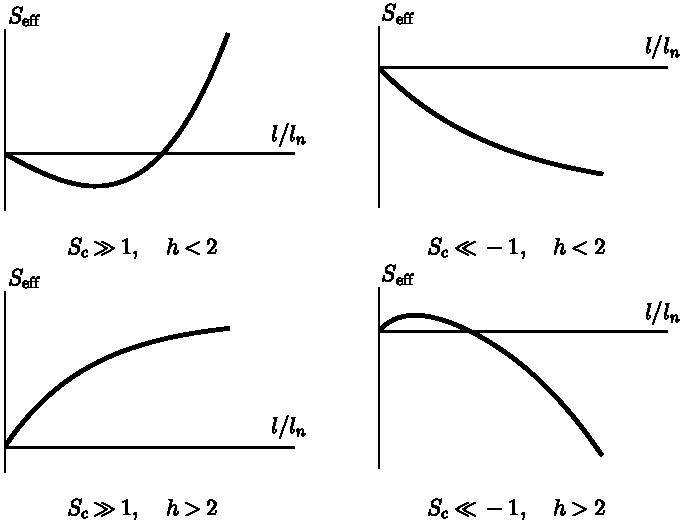
\includegraphics[width=0.72\textwidth]{fig_3.8.pdf}
\caption*{图 3.8\quad $S_{\mathrm{eff}}$ 作为 $l/l_{n}$ 的函数。四个面板分别对应 $S_{c}\gg 1,\ h<2$；$S_{c}\ll -1,\ h<2$；$S_{c}\gg 1,\ h>2$；$S_{c}\ll -1,\ h>2$。}
\end{figure}
为了理解涡旋的效应，让我们估计 $n$ 个涡旋与 $n$ 个反涡旋的配分函数，即 $Z = \mathrm{e}^{-S_{\mathrm{eff}}}$，其中
\begin{equation*}
S_{\mathrm{eff}} \sim 2n\ln n + n\left(2h\ln\frac{l_{n}}{l} + 2S_{c}\right) - 2n\ln\frac{L^{2}}{l^{2}}
= L^{2}\frac{2}{l_{n}^{2}}(h-2)\ln\frac{l_{n}\mathrm{e}^{S_{c}/(h-2)}}{l}
\tag{3.4.6}
\end{equation*}
其中 $L$ 是系统的线性尺寸，$l_{n} = L/\sqrt{n}$ 是涡旋之间的平均间距。这里 $l_{n}$ 总是大于截断，即 $l_{n} > l$。式 (3.4.6) 的第一项来自 $1/(n!)^{2}$。第二项是 $n$ 对涡旋--反涡旋的作用量，每对占据大小 $\sim l_{n}$ 的一块面积。它包含两项贡献：涡旋相互作用 $2h\ln\frac{l_{n}}{l}$ 和芯部作用量 $2S_{c}$。第三项来自对涡旋位置的积分 $\int \prod_{i=1}^{2n}\mathrm{d}^{2}\pmb{r}_{i}$（它就是熵）。涡旋气体的行为由涡旋作用量（倾向于更少的涡旋）与熵（倾向于更多的涡旋）之间的竞争控制。

涡旋的数目 $n$ 可以这样简单地得到：在 $l_{n} > l$ 的范围内对 $l_{n}$ 极小化 $S_{\mathrm{eff}}$。从图 3.8 中 $S_{\mathrm{eff}}$ 的行为我们看到，当 $S_{c} \ll -1$（即产生涡旋的代价很低）时，$S_{\mathrm{eff}}$ 在边界 $l_{n} \sim l$ 处取极小。在这种情况下，涡旋涨落是重要的，它把式 (3.4.4) 中的代数长程序变为短程序：
\begin{equation*}
\left\langle \mathrm{e}^{\mathrm{i}\theta(\pmb{x})}\mathrm{e}^{-\mathrm{i}\theta(0)} \right\rangle \sim \mathrm{e}^{-|\pmb{x}|/\xi}
\end{equation*}
关联长度为 $\xi \sim l_{n} \sim l$。

当 $S_{c} \gg 1$ 且 $h = \pi\eta < 2$ 时，$S_{\mathrm{eff}}$ 在 $l_{n} \sim \mathrm{e}^{S_{c}/(2-h)}l$ 处取极小。此时涡旋密度仍然是有限的，这同样把代数长程序变为

% ---- 书页 104 (p119) ----
\begin{figure}[H]
\centering
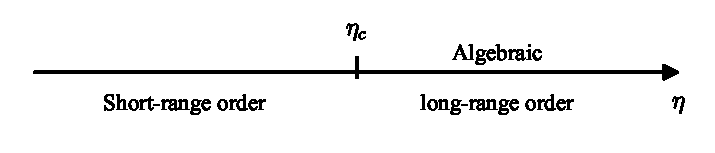
\includegraphics[width=0.72\textwidth]{fig_3.9.pdf}
\caption*{图 3.9\quad 二维 XY 模型的相图。横轴为 $\eta$，在 $\eta_{c}$ 之左为短程序，之右为代数长程序。}
\end{figure}
短程序。关联长度为
\begin{equation*}
\xi \sim l_{n} \sim l\,\mathrm{e}^{S_{c}/(2-h)}
\tag{3.4.7}
\end{equation*}
当 $S_{c} \gg 1$ 且 $h = \pi\eta > 2$ 时，$S_{\mathrm{eff}}$ 在 $l_{n} = \infty$ 处取极小，涡旋密度为零。在这种情况下，涡旋涨落在长距离下并不重要，代数长程序可以在涡旋涨落下存活。

从上面的讨论我们看到，在 $S_{c} \gg 1$ 极限下，随着我们改变 $\eta$，二维玻色系统经历一个有限温度相变。该相变把代数长程序变为短程序。相变处的临界 $\eta$ 为 $\eta_{c} = 2/\pi$。图 3.9 中的相图总结了我们在 $S_{c} \gg 1$ 极限下的结果。$\eta_{c}$ 处的相变就是著名的 Kosterlitz--Thouless（KT）相变。利用 $\eta$ 与 $T$ 之间的关系 (3.4.3)，我们求得临界温度
\begin{equation*}
T_{KT} = \frac{\pi\varphi_{0}}{2m}
\end{equation*}
我们想指出，KT 相变不改变任何对称性，因而是 Landau 关于相与相变的对称性破缺理论的一个反例。

利用 $h = \pi\eta = \pi\varphi_{0}^{2}/mT$，式 (3.4.7) 可以改写为
\begin{equation*}
\xi(T) \sim l\,\mathrm{e}^{E_{\xi}/(T-T_{KT})}
\tag{3.4.8}
\end{equation*}

\begin{smallnote}
在 $T_{KT}$ 附近，其中 $E_{\xi}$ 是某个能量尺度。这里我们想指出，当 $T \to T_{KT}$ 时式 (3.4.8) 并不正确。这个不正确的结果来自一个不正确的假设，即相位劲度 $\eta$ 不受涡旋存在的影响。事实上，涡旋气体会修改 $\eta$ 和 $h$ 的有效值。这是因为涡旋--反涡旋对可以被相位扭转 $\partial_{\pmb{x}}\theta$ 极化，从而释放部分应变并降低有效相位劲度。采用有效值 $h^{*}$，式 (3.4.7) 应当改写为
\begin{equation*}
\xi \sim l_{n} \sim l\,\mathrm{e}^{S_{c}/(2-h^{*})}
\tag{3.4.9}
\end{equation*}
$h^{*}(T)$ 的温度依赖性比 $h(T)$ 的更为复杂。不过，按定义 $h^{*}(T_{KT}) = 2$。基于一个重整化群计算（见 3.5.6 节），我们发现
\begin{equation*}
2 - h^{*}(T_{KT}) \propto (T - T_{KT})^{1/2}
\end{equation*}
（译注：原文括号内印作 $T_{TK}$，应为 $T_{KT}$。）
由此得到
\begin{equation*}
\xi(T) \sim l\,\mathrm{e}^{\left(E_{\xi}/(T-T_{KT})\right)^{1/2}}
\tag{3.4.10}
\end{equation*}
\end{smallnote}

% ---- 书页 105 (p120) ----
\subsection*{问题 3.4.1}
注意到，在 $T_{c}$ 附近，式 (3.4.1) 中的作用量 $S_{\mathrm{eff}}$ 可以近似为
\begin{equation*}
S_{\mathrm{eff}} = \beta\int \mathrm{d}^{d}\pmb{x}\ \left[ \frac{1}{2m^{*}}|\partial_{\pmb{x}}\varphi_{c}|^{2} + a(T-T_{c})|\varphi_{c}|^{2} + b|\varphi_{c}|^{4} \right] + O(|\varphi_{c}|^{6})
\end{equation*}
因为在 $T = T_{c}$ 处的临界点（或相变点）附近序参量 $\varphi_{c}$ 很小。在用平均场（或半经典）方法处理相变和临界点时，我们首先求出使作用量取极小的平均场解，然后假设平均场解附近的涨落很小，把作用量展开到涨落的二次阶。$S_{\mathrm{eff}}$ 的二次近似可以用来计算各种关联函数。

\begin{enumerate}
\item 用平均场方法计算临界点处 $\langle \varphi_{c}(\pmb{x})\varphi_{c}^{*}(0)\rangle \sim 1/|\pmb{x}|^{\gamma}$ 中的衰减指数 $\gamma$。
\item 上述结果并非总是成立，因为经典理论可能会失效。重复 3.3.8 节末尾的讨论（即把 $S_{\mathrm{eff}}$ 写成 $g^{-1}\tilde{S}$ 的形式，$\tilde{S}$ 无量纲），看看平均场方法何时能正确描述临界点、何时临界点由强涨落控制；也就是说，求出上临界点 $d_{c}$。
\item 这里我们想引入相关微扰与不相关微扰的概念。我们知道，在上临界维数以上，经典理论能正确描述相变处的临界点。现在我们在有效作用量 $S_{\mathrm{eff}}$ 中加一个微扰 $\beta\int \mathrm{d}^{d}x\ c|\varphi|^{\sigma}$。如果该微扰是重要的并且修改临界指数，我们就称它为相关微扰（relevant perturbation）；如果该微扰在临界点附近变得任意小，我们就称它为不相关微扰（irrelevant perturbation）。利用你在上面找到的同样的标度关系，考察微扰 $\beta\int \mathrm{d}^{d}x\ c|\varphi|^{\sigma}$ 如何修改标度后的作用量 $\tilde{S}$。确定 $\sigma$ 在什么范围内该微扰是相关的，在什么范围内是不相关的。
\end{enumerate}

\section{重整化群}

\subsection{相关微扰与不相关微扰}
\begin{keypoints}
\item 相关微扰改变系统的长距离（或低能）行为，而不相关微扰不改变。
\item 我们可以利用微扰的标度量纲来判断该微扰是相关的还是不相关的。
\end{keypoints}

在上面关于 KT 相变的讨论中我们注意到，当 $\mathrm{e}^{-S_{c}} \ll 1$ 时，涡旋涨落只是“小微扰”。然而，如果 $h < 2$，那么无论 $\mathrm{e}^{-S_{c}}$ 多么小，涡旋涨落总会破坏 $\langle \mathrm{e}^{\mathrm{i}\theta(\pmb{x})}\mathrm{e}^{-\mathrm{i}\theta(0)}\rangle$ 的代数长程关联。因此，当 $h<2$ 时，把涡旋涨落包括进来这一微扰被称为相关微扰。当 $h>2$ 时，该微扰被称为不相关微扰；而当 $h=2$ 时，该微扰被称为边缘微扰（marginal perturbation）。下面我们想在更一般的框架中讨论相关/不相关/边缘微扰。

% ---- 书页 106 (p121) ----
考虑一个由作用量
\begin{equation*}
S = S_{0} + \int \mathrm{d}^{d}x\ aO(x)
\end{equation*}
描写的理论，其中 $aO$ 是一个微扰。我们假设 $S_{0}$ 具有 $Z_{2}$ 对称性，且在 $Z_{2}$ 变换下 $O \to -O$。于是，当 $a=0$ 时 $\langle O\rangle = 0$。我们还假设，对于大的 $x$，在 $a=0$ 时
\begin{equation*}
\langle O(x)O(0)\rangle = \frac{1}{|x|^{2h}}
\tag{3.5.1}
\end{equation*}
这里 $h$ 称为算符 $O$ 的标度量纲（scaling dimension，$1/x$ 的标度量纲定义为 1）。式 (3.5.1) 同时也定义了算符 $O$ 的归一化。

在二阶微扰下，配分函数由下式给出
\begin{equation*}
Z = Z_{0} \int \mathrm{d}^{d}x\,\mathrm{d}^{d}y\ a^{2}\langle O(x)O(y)\rangle
\end{equation*}
其中 $Z_{0}$ 是零阶配分函数。我们看到，二阶微扰对有效作用量的改变为
\begin{equation*}
\Delta S_{\mathrm{eff}} = -\ln Z + \ln Z_{0} = -2\ln g + 2h\ln L - 2d\ln L
\end{equation*}
（译注：原文 $\ln g$ 按上下文应为 $\ln a$。）

注意到，当 $h < d$ 且 $L > \xi = a^{-1/(d-h)}$ 时，我们有 $\Delta S_{\mathrm{eff}} < 0$。因此，系统倾向于有两个 $O(x)$ 插入。当 $L \gg \xi$ 时，系统希望在每个 $\xi^{d}$ 体积内有两个 $O(x)$ 插入。我们看到，如果我们感兴趣的是 $\xi$ 之外长度尺度上的关联函数，那么该微扰总是重要的。我们得出结论：如果 $O(x)$ 的标度量纲小于 $d$，则微扰 $\int \mathrm{d}^{d}x\ O(x)$ 是相关的。此时 $O(x)$ 称为相关算符。如果 $O(x)$ 的标度量纲大于（或等于）$d$，则 $O(x)$ 称为不相关（边缘）算符。记住这个结果的一个简单办法是：注意若 $\int \mathrm{d}^{d}x\ O(x)$ 的量纲小于零，则微扰 $\int \mathrm{d}^{d}x\ O(x)$ 是相关的。

标度量纲的概念还使我们能够用量纲分析来估计有限微扰 $aO$ 所诱导的 $\langle O\rangle$。由于 $\delta S = \int \mathrm{d}^{d}x\ aO$ 的标度量纲按定义为零，系数 $a$ 具有标度量纲 $[a] = d - [O] = d - h$。当 $aO$ 是不相关微扰（即 $h > d$）时，诱导的 $\langle O\rangle$ 正比于 $a$。我们有
\begin{equation*}
\langle O\rangle \sim a\,l^{d-2h}
\end{equation*}
其中 $l$ 是短距离截断。当 $aO$ 是相关微扰（即 $h < d$）时，诱导的 $\langle O\rangle$ 大于 $a\,l^{d-2h}$。通过匹配标度量纲，

% ---- 书页 107 (p122) ----
我们求得
\begin{equation*}
\langle O\rangle \sim a^{h/(d-h)} = a\xi^{d-2h}.
\tag{3.5.2}
\end{equation*}

\subsection*{问题 3.5.1}
有效作用量
\begin{equation*}
S_{\mathrm{eff}} = \beta\int \mathrm{d}^{d}\pmb{x}\ \frac{1}{2m^{*}}|\partial_{\pmb{x}}\varphi|^{2}
\end{equation*}
描写一个临界点。计算 $\varphi$、$\varphi^{2}$、$|\varphi|^{2}$ 和 $|\varphi|^{4}$ 的标度量纲。证明：在某个空间维度 $d_{0}$ 以下，微扰 $\int \mathrm{d}^{d}\pmb{x}\ b|\varphi|^{4}$ 成为相关微扰。求出 $d_{0}$ 的值，并解释为什么 $d_{0}$ 等于
\begin{equation*}
S_{\mathrm{eff}} = \beta\int \mathrm{d}^{d}\pmb{x}\ \left[ \frac{1}{2m^{*}}|\partial_{\pmb{x}}\varphi|^{2} + a(T-T_{c})|\varphi|^{2} + b|\varphi|^{4} \right]
\end{equation*}
的上临界维数 $d_{c}$。

\subsection{二维 XY 模型与二维时钟模型之间的对偶}
\begin{keypoints}
\item 二维 XY 模型中的涡旋可以看作粒子。描写这些粒子的场论是二维时钟模型（clock model）。
\end{keypoints}

为了更仔细地研究 XY 模型的涡旋涨落，我们想把二维 XY 模型映射到 $Z_{1}$ 二维时钟模型。一个一般的 $Z_{n}$ 时钟模型定义为
\begin{equation*}
S = \int \mathrm{d}^{2}\pmb{x}\ \left( \frac{\kappa}{2}(\partial_{\pmb{x}}\theta)^{2} - g\cos(n\theta) \right)
\tag{3.5.3}
\end{equation*}
当 $g = 0$ 时，时钟模型就是有限温度下的 XY 模型。作用量是能量除以温度：$S = \beta E$。$g\cos(n\theta)$ 项（显式地）破坏 $U(1)$ 转动对称性。如果我们把 $(\cos(\theta), \sin(\theta)) = (S_{x}, S_{y})$ 看作自旋的两个分量，那么对于 $n = 1$，$g\cos(\theta)$ 项就是由 $S_{x}$ 方向的磁场诱导的项。对于一般的 $n$，时钟模型具有 $Z_{n}$ 对称性：$\theta \to \theta + \frac{2\pi}{n}$。

为了证明对偶关系，我们考虑式 (3.5.3) 在 $n = 1$ 时的配分函数：
\begin{equation*}
\begin{aligned}
Z &= \int \mathcal{D}\theta\ \sum_{k} \frac{1}{k!}\left( g\int \mathrm{d}^{2}x\ \frac{\mathrm{e}^{\mathrm{i}\theta} + \mathrm{e}^{-\mathrm{i}\theta}}{2} \right)^{k} \mathrm{e}^{-\int \mathrm{d}^{2}\pmb{x}\ \frac{\kappa}{2}(\partial_{\pmb{x}}\theta)^{2}} \\
&= Z_{0} \sum_{k} \frac{1}{k!k!} \int \prod_{i=1}^{2k} \mathrm{d}^{2}\pmb{r}_{i}\ \mathrm{e}^{-2kS_{c}}\ \mathrm{e}^{\sum_{i<j}^{2k} 2hq_{i}q_{j}\ln\frac{r_{ij}}{l}}
\end{aligned}
\tag{3.5.4}
\end{equation*}
其中 $Z_{0}$ 是 $S = \int \mathrm{d}^{2}\pmb{x}\ \frac{\kappa}{2}(\partial_{\pmb{x}}\theta)^{2}$ 的配分函数。求和中的每一项来自关联 $\langle \mathrm{e}^{\mathrm{i}\theta(\pmb{r}_{1})}\allowbreak\ldots\allowbreak\mathrm{e}^{\mathrm{i}\theta(\pmb{r}_{k})}\allowbreak\mathrm{e}^{-\mathrm{i}\theta(\pmb{r}_{k+1})}\allowbreak\ldots\allowbreak\mathrm{e}^{-\mathrm{i}\theta(\pmb{r}_{2k})}\rangle$。此外，

% ---- 书页 108 (p123) ----
$q_{i} = 1$（当 $1 \leqslant i \leqslant k$），$q_{i} = -1$（当 $k+1 \leqslant i \leqslant 2k$），$\mathrm{e}^{-S_{c}} = g/2$，以及
\begin{equation*}
h = \frac{1}{4\pi\kappa}
\end{equation*}
（译注：原文 $q_{i} = -1$ 的条件印作 $k+1 \leqslant i \leqslant 2n$，应为 $2k$。）

如果 $\frac{1}{4\pi\kappa} = \pi\eta$，则式 (3.5.4) 与 XY 模型 (3.4.2) 的配分函数 (3.4.5) 完全相同。所以，当 $\frac{1}{2\pi\kappa} = 2\pi\eta$ 时，$Z_{1}$ 时钟模型 (3.5.3) 等价于（带涡旋的）XY 模型 (3.4.2)。XY 模型中的涡旋被映射到时钟模型中的 $\mathrm{e}^{\mathrm{i}\theta(\pmb{x})}$。类似地，时钟模型中的涡旋被映射到 XY 模型中的 $\mathrm{e}^{\mathrm{i}\theta(\pmb{x})}$。时钟模型中的涡旋具有标度量纲 $\pi\kappa$，而 XY 模型中的 $\mathrm{e}^{\mathrm{i}\theta(\pmb{x})}$ 算符具有标度量纲 $1/4\pi\eta$。关系 $\frac{1}{2\pi\kappa} = 2\pi\eta$ 保证了这两个标度量纲彼此一致。

我们知道，XY 模型中的 $U(1)$ 对称性不允许 $\mathrm{e}^{\mathrm{i}\theta}$ 项出现在作用量中。利用上述映射我们看到，相应的时钟模型必须不允许涡旋涨落。在时钟模型中允许涡旋涨落，对应于在对偶的 XY 模型中显式破坏 $U(1)$ 对称性。我们看到，时钟模型有两种不同的类型：允许涡旋涨落的一种和不允许涡旋涨落的一种。由于相应的对偶模型具有不同的对称性，这两种时钟模型具有非常不同的性质。我们把允许涡旋涨落的时钟模型称为紧致时钟模型（compact clock model），把不允许涡旋涨落的称为非紧致时钟模型（non-compact clock model）。带涡旋的 XY 模型被映射到一个 $Z_{1}$ 非紧致时钟模型。这样的映射使我们能够通过研究相应非紧致时钟模型中的相变来研究 XY 模型中的 KT 相变。

\subsection{时钟模型的物理性质}
\begin{keypoints}
\item 除非指定短距离截断，一个场论模型是没有良定义的。
\item 包含强涡旋涨落的 Ginzburg--Landau 理论不能描述非紧致时钟模型中的相变。
\end{keypoints}

本节中，我们将讨论一般的 $Z_{n}$ 时钟模型中可能的相变。当 $g$ 大时，场 $\theta$ 被势 $-g\cos(n\theta)$ 的某个极小值俘获。我们相信，此时模型处于一个自发破缺 $Z_{n}$ 对称性的相。当 $\kappa$ 和 $g$ 都小时，$\theta$ 的涨落很强。我们预期模型将处于 $Z_{n}$ 对称相。

尽管听起来相当合理，上述说法其实并没有真正的意义。这是因为 $g$ 具有量纲，谈论 $g$ 有多大是没有意义的。更糟的是，$g$ 是模型中唯一具有非平凡量纲的参量，所以我们无法构造一个无量纲组合来判断 $g$ 有多大。

% ---- 书页 109 (p124) ----
为了以物理的方式理解 $g\cos(n\theta)$ 项的重要性，我们想问 $\mathrm{e}^{\mathrm{i}n\theta}$ 算符有多大。回答这个问题的一个物理办法，是考察 XY 模型 $S = \int \mathrm{d}^{2}\pmb{x}\ \frac{\kappa}{2}(\partial_{\pmb{x}}\theta)^{2}$ 中 $\mathrm{e}^{\mathrm{i}n\theta}$ 的关联。该关联由下式给出（见式 (3.3.25)）
\begin{equation*}
\left\langle \mathrm{e}^{\mathrm{i}n\theta(\pmb{x})}\mathrm{e}^{-\mathrm{i}n\theta(0)} \right\rangle = (l/|\pmb{x}|)^{n^{2}/2\pi\kappa}
\tag{3.5.5}
\end{equation*}
一个大的意外是，该关联依赖于短距离截断 $l$。这样一来，算符 $\mathrm{e}^{\mathrm{i}n\theta}$ 的大小（或重要性）在未指定截断 $l$ 之前甚至没有良定义。这说明了这样一点：\emph{要有一个良定义的场论，我们必须指定一个短距离截断 $l$}。为了强调这一点，我们想把 $l$ 依赖性显式地写出来，把作用量写成
\begin{equation*}
S = \int \mathrm{d}^{2}\pmb{x}\ \left( \frac{\kappa_{l}}{2}(\partial_{\pmb{x}}\theta_{l})^{2} - g_{l}\cos(n\theta_{l}) \right)
\tag{3.5.6}
\end{equation*}
短距离截断是这样引入的：要求 $\theta_{l}$ 场不包含任何波长短于 $l$ 的涨落：
\begin{equation*}
\theta_{l}(\pmb{x}) = \int_{|\pmb{k}|<2\pi/l} \mathrm{d}^{2}\pmb{k}\ \theta_{\pmb{k}}\mathrm{e}^{\mathrm{i}\pmb{x}\cdot\pmb{k}}
\end{equation*}
我们看到，良定义的时钟模型 (3.5.6) 包含三个参量 $\kappa_{l}$、$g_{l}$ 和 $l$。所以，时钟模型实际上包含两个无量纲参量 $\kappa_{l}$ 和 $\bar{g}_{l} = g_{l}l^{2}$。

现在我们可以做有意义的陈述了。当 $\bar{g}_{l} \gg 1$ 时，我们相信模型处于自发破缺 $Z_{n}$ 对称性的相。当 $\kappa_{l}$ 和 $\bar{g}_{l}$ 都远小于 1 时，我们预期模型处于 $Z_{n}$ 对称相。

一个非平凡的极限是 $\kappa_{l} \gg 1$ 且 $\bar{g}_{l} \ll 1$。此时模型是处于 $Z_{n}$ 对称相还是 $Z_{n}$ 对称性破缺相？相关/不相关微扰的概念对回答这个问题非常有帮助。如果我们把 $g_{l}\cos(n\theta)$ 项当作 XY 模型的微扰，那么由式 (3.5.5)，XY 模型中 $\mathrm{e}^{\mathrm{i}n\theta}$ 的标度量纲为 $[\mathrm{e}^{\mathrm{i}n\theta}] = n^{2}/4\pi\kappa_{l}$。因此，$g_{l}\cos(n\theta)$ 项在 $n^{2}/4\pi\kappa_{l} < 2$ 时是相关的，在 $n^{2}/4\pi\kappa_{l} > 2$ 时是不相关的。

这个结果是合理的。当 $\kappa_{l}$ 小时，$\theta$ 的涨落强。这使得 $g_{l}\cos(n\theta)$ 项平均为零，效果减弱。因此微扰 $g_{l}\cos(n\theta)$ 是不相关的。当 $g_{l}\cos(n\theta)$ 不相关且 $\bar{g}_{l}$ 小时，我们在计算长程关联时可以丢掉 $g_{l}\cos(n\theta)$ 项。这表明，在 $\kappa_{l}$ 和 $\bar{g}_{l}$ 都小时，长距离下我们不仅有 $Z_{n}$ 对称性，还有完整的 $U(1)$ 对称性。

当 $\kappa$ 大时，$\theta$ 的涨落弱。这使得 $g_{l}\cos(n\theta)$ 项成为相关微扰。此时无论 $\bar{g}_{l}$ 多么小，$g_{l}\cos(n\theta)$ 项的效应都会在长距离下变得重要。

% ---- 书页 110 (p125) ----
这样，我们预期系统被俘获在势项的 $n$ 个极小之一中，$Z_{n}$ 对称性自发破缺，即使 $\bar{g}_{l}$ 很小。

在认识到时钟模型可以有 $Z_{n}$ 对称性破缺相和 $Z_{n}$ 对称相之后，下一个自然的问题是：这两相之间如何相互转化？理解这种相变的一个办法，是引入复序参量 $\varphi(\pmb{x}) = \langle \mathrm{e}^{\mathrm{i}\theta(\pmb{x})}\rangle$，并写下相变的 Ginzburg--Landau 有效理论
\begin{equation*}
S_{GL} = \int \mathrm{d}^{2}\pmb{x}\ \left[ \frac{\gamma}{2}(\partial_{\pmb{x}}\varphi)^{2} + a|\varphi|^{2} + b|\varphi|^{4} - c\,\mathrm{Re}\,\varphi^{n} \right]
\tag{3.5.7}
\end{equation*}
注意到，$c\,\mathrm{Re}\,\varphi^{n}$ 项（显式地）把 $U(1)$ 对称性破缺到 $Z_{n}$。当 $n > 1$ 时，随着 $a$ 从正值变为负值，Ginzburg--Landau 理论描述了一个对称性破缺相变。

当 $n = 1$ 时，Ginzburg--Landau 理论不包含相变，因为没有对称性破缺。这似乎暗示 $Z_{1}$ 时钟模型不包含相变，而相应的 XY 模型不包含 KT 相变。

那么问题出在哪里？在 Ginzburg--Landau 理论中，序参量在相变点附近有很强的振幅涨落。$\varphi$ 的一个典型位形包含许多 $\varphi = 0$ 的点，所以存在很强的涡旋涨落。Ginzburg--Landau 理论描述的是紧致时钟模型中的相变，它不适用于非紧致时钟模型。

\subsection{非紧致时钟模型的重整化群方法}
\begin{keypoints}
\item 通过跑动耦合常数（running coupling constants）的概念，重整化群（RG）方法使我们能够看到，当我们走向长距离或低能量时理论如何演化。它非常有用，因为它告诉我们哪些动力学性质在长距离或低能量下演生。
\item 由于一个有效理论只会演化成相似的有效理论，我们无法用重整化群方法得到性质上全新的现象的演生，例如从玻色模型演生出光和费米子。
\end{keypoints}

本节中，为了理解非紧致时钟模型的物理性质，我们将直接处理时钟模型中的 $\theta$ 场。

我们注意到，如果不同位置处的涨落 $O(\pmb{x})$ 与 $O(\pmb{y})$ 彼此独立地涨落，那么所谓的\emph{连通关联}（connected correlation）
\begin{equation*}
G_{\mathrm{conn}} = \langle O(\pmb{x})O(\pmb{y})\rangle - \langle O(\pmb{x})\rangle\langle O(\pmb{y})\rangle
\end{equation*}

% ---- 书页 111 (p126) ----
为零。所以，连通关联度量的正是 $O(\pmb{x})$ 与 $O(\pmb{y})$ 的涨落之间的关联。

当 $g_{l} = 0$ 时，无论 $\kappa_{l}$ 取何值，非紧致时钟模型总是具有代数长程关联：$\langle \mathrm{e}^{\mathrm{i}n\theta(\pmb{x})}\mathrm{e}^{-\mathrm{i}n\theta(0)}\rangle - \langle \mathrm{e}^{\mathrm{i}n\theta(\pmb{x})}\rangle\langle \mathrm{e}^{-\mathrm{i}n\theta(0)}\rangle \sim \frac{1}{|\pmb{x}|^{n^{2}/2\pi\kappa_{l}}}$。这里的问题是，$g_{l}\cos(n\theta)$ 项会如何影响代数长程关联。

如上一节所讨论，当 $\kappa_{l} < n^{2}/8\pi$ 时，$\mathrm{e}^{\mathrm{i}n\theta(\pmb{x})}$ 是不相关的，小的 $g_{l}\cos(n\theta)$ 项不会影响代数长程关联。当 $\kappa_{l} > n^{2}/8\pi$ 时，$\mathrm{e}^{\mathrm{i}n\theta(\pmb{x})}$ 是相关的。我们预期，无论 $\bar{g}_{l}$ 多么小，$g_{l}\cos(n\theta)$ 项都会把代数长程关联变为短程关联。我们看到，对于小的 $\bar{g}_{l}$，非紧致时钟模型在 $\kappa_{l} = n^{2}/8\pi$ 处有一个相变。下面我们将用 RG 方法来理解这个相变。

我们注意到，只有在指定了短距离截断 $l$ 之后，时钟模型才是良定义的。RG 方法的关键一步，是把波长介于 $l$ 与 $\lambda$（$\lambda > l$）之间的涨落积掉。这得到一个具有新截断 $\lambda$ 的模型。为了把短波长 $\theta$ 涨落积掉，我们先写
\begin{equation*}
\theta_{l} = \theta_{\lambda} + \delta\theta
\end{equation*}
其中 $\delta\theta$ 只包含波长介于 $l$ 与 $\lambda$ 之间的涨落。由于短波长涨落 $\delta\theta$ 受到 $\kappa(\partial_{\pmb{x}}\delta\theta)^{2}$ 项的压制，我们预期 $\delta\theta$ 很小，并把作用量展开到 $\delta\theta$ 的二阶：
\begin{equation*}
\begin{aligned}
S = {} & \int \mathrm{d}^{2}\pmb{x}\ \left( \frac{\kappa_{l}}{2}(\partial_{\pmb{x}}\theta_{\lambda})^{2} - g_{l}\cos(n\theta_{\lambda}) + \frac{\kappa_{l}}{2}(\partial_{\pmb{x}}\delta\theta)^{2} \right) \\
& + \int \mathrm{d}^{2}\pmb{x}\ \left( -ng_{l}\sin(\theta_{\lambda})\delta\theta + \frac{n^{2}}{2}g_{l}\cos(n\theta_{\lambda})(\delta\theta)^{2} \right)
\end{aligned}
\end{equation*}
（译注：原文 $\sin(\theta_{\lambda})$ 按展开式应为 $\sin(n\theta_{\lambda})$。）

我们把 $\theta_{\lambda}$ 当作光滑的背景场，并把 $\delta\theta$ 积掉（这种方法称为背景场 RG 方法）。我们得到有效作用量
\begin{equation*}
\begin{aligned}
S = {} & \int \mathrm{d}^{2}\pmb{x}\ \left( \frac{\kappa_{l}}{2}(\partial_{\pmb{x}}\theta_{\lambda})^{2} - g_{l}\cos(n\theta_{\lambda}) + \frac{1}{2}g_{l}\cos(n\theta_{\lambda})K(0) \right) \\
& - \int \mathrm{d}^{2}\pmb{x}\,\mathrm{d}^{2}\pmb{y}\ \frac{1}{2}(g_{l})^{2}\sin(n\theta_{\lambda}(\pmb{x}))K(\pmb{x}-\pmb{y})\sin(n\theta_{\lambda}(\pmb{y}))
\end{aligned}
\end{equation*}
% ——— 块边界说明（起点）———
% 书页 111（p126）末行为 §3.5.4 的无编号有效作用量
%   S = ∫d²x(κ_l/2(∂_xθ_λ)² − g_l cos(nθ_λ) + ½g_l cos(nθ_λ)K(0))
%     − ∫d²x d²y ½(g_l)²sin(nθ_λ(x))K(x−y)sin(nθ_λ(y))，
% 本块自书页 112（p127）顶部残句 "where K(x) = n²⟨δθ(x)δθ(0)⟩. We note that
% the last term can be rewritten as" 续起，上面 %JOIN% 使本块与 ch3_d 末式直接缝合。
% ——— 块边界说明（终点）———
% 书页 122（p137）末句 "Let us consider the spectral expansion" 跨页延续到
% 书页 123（p138）顶部 "of the density correlation function:"。按 assemble.py
% 约定（X 文件的 %--XX-TAIL-- 区内容会移到 X−1 之后、X 正文之前），该残句的
% 译文（"密度关联函数的谱展开："）应由 ch3_f 写入其 %--E-TAIL-- 区（或在其
% 正文开头以 %JOIN% 续译），本块正文因此止于"让我们考虑"，本文件不设
% %--D-TAIL-- 区。ch3_f 请勿重复翻译该残句；其正文请从 p138 顶部的谱展开
% 无编号式 ⟨ρ(t,x)ρ(0,0)⟩ = ⟨0|ρ(x)U(t,0)ρ(0)|0⟩/⟨0|U(t,0)|0⟩ = … 起译。
% ——————————————————————————————
其中，$K(\pmb{x}) = n^2\langle\,\delta\theta(\pmb{x})\,\delta\theta(0)\rangle$。我们注意到，最后一项可以改写为
\begin{align*}
&\int \mathrm{d}^2\pmb{x}\,\mathrm{d}^2\pmb{y}\,\frac{g_l^2}{4}[\sin(n\theta_\lambda(\pmb{x})) - \sin(n\theta_\lambda(\pmb{y}))]^2 K(\pmb{x}-\pmb{y}) - \int \mathrm{d}^2\pmb{x}\,\frac{g_l^2}{2}\sin^2(n\theta_\lambda)\bar{K} \\
={}& \int \mathrm{d}^2\pmb{x}\,\mathrm{d}^2\pmb{y}\,\frac{n^2}{8}(g_l)^2\cos^2(n\theta_\lambda(\pmb{x}))(\partial_{\pmb{x}}\theta_\lambda(\pmb{x}))^2(\pmb{x}-\pmb{y})^2 K(\pmb{x}-\pmb{y}) \\
&- \int \mathrm{d}^2\pmb{x}\,\frac{1}{2}(g_l)^2(\sin(n\theta_\lambda(\pmb{x})))^2\bar{K}
\end{align*}
其中，$\bar{K} = \int \mathrm{d}^2\pmb{x}\,K(\pmb{x})$。我们看到，像 $\cos(2n\theta_\lambda)$、$(\partial_{\pmb{x}}\theta_\lambda)^2$、$\cos(2n\theta_\lambda)(\partial_{\pmb{x}}\theta_\lambda)^2$、$(\partial_{\pmb{x}}\theta_\lambda)^4$ 等等这样的项被产生了出来。RG 流可以产生许多初始作用量中没有的新项。事实上，任何不破坏 $Z_n$ 对称性的局域项都可能被产生。然而，$\cos(\theta_\lambda)$ 项在 $n>1$ 时不会被产生，因为它破坏 $Z_n$ 对称性。目前，让我们只保留初始作用量中已有的 $(\partial_{\pmb{x}}\theta_\lambda)^2$ 与 $\cos(\theta_\lambda)$ 两项。\footnote{事实证明，所有其他项都是不相关的。如果这些项在 RG 流开始时很小，那么经过长时间流动后它们会变得更小。这就是我们可以忽略这些项的原因。当然，如果这些项一开始就很大，那么它们可以改变一切。}我们发现，模型的作用量变为
\begin{equation*}
S = \int \mathrm{d}^2\pmb{x}\left(\frac{\kappa_\lambda}{2}(\partial_{\pmb{x}}\theta_\lambda)^2 - g_\lambda\cos(n\theta_\lambda)\right)\tag{3.5.8}
\end{equation*}
其中 $\lambda$ 是新的截断。有效耦合常数依赖于截断 $\lambda$，称为跑动耦合常数（running coupling constants）。它们由下式给出（假定 $\frac{\lambda-l}{l}\ll 1$）
\begin{equation*}
g_\lambda = g_l - \frac{1}{2}K(0),\qquad \kappa_\lambda = \kappa_l + \frac{n^2}{8}g_l^2 K_2
\end{equation*}
\begin{equation*}
K(0) = \int_{2\pi/\lambda < |\pmb{k}| < 2\pi/l} \frac{\mathrm{d}^2\pmb{k}}{(2\pi)^2}\,\frac{n^2}{\kappa_l|\pmb{k}|^2} = \frac{n^2}{2\pi\kappa_l}\ln\frac{\lambda}{l}
\end{equation*}
\begin{align*}
K_2 &\equiv \int \mathrm{d}^2\pmb{x}\,|\pmb{x}|^2 K(\pmb{x}) = \int_{2\pi/\lambda < |\pmb{k}| < 2\pi/l} \mathrm{d}^2\pmb{x}\,\frac{\mathrm{d}^2\pmb{k}}{(2\pi)^2}\,\frac{n^2\pmb{x}^2\,\mathrm{e}^{\mathrm{i}\pmb{k}\cdot\pmb{x} - 0^+|\pmb{x}|}}{\kappa_l\pmb{k}^2} \\
&= \frac{\lambda-l}{l}\,\frac{3n^2l^4}{16\pi^5\kappa_l}\int \mathrm{d}\theta\,\frac{1}{(\cos\theta + \mathrm{i}0^+)^4} = \frac{\lambda-l}{l}\,\frac{3n^2l^4}{2\pi^4\kappa_l}
\end{align*}

\begin{figure}[H]
\centering
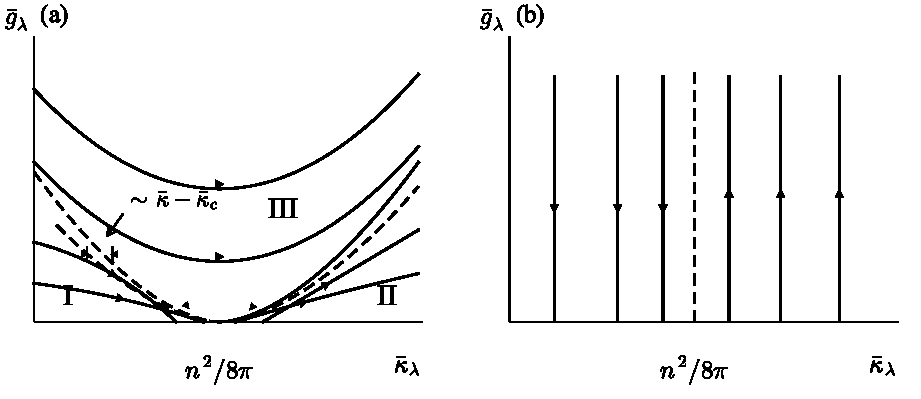
\includegraphics[width=0.72\textwidth]{fig_3.10.pdf}
\caption*{图 3.10\quad (a) 由式 (3.5.9) 确定的 $g_\lambda$ 与 $\kappa_\lambda$ 的重整化群流。(b) 由式 (3.5.10) 确定的 $g_\lambda$ 与 $\kappa_\lambda$ 的重整化群流。}
\end{figure}

令 $b = \ln\lambda$，则耦合常数的变化由下列微分方程描述：
\begin{align*}
\frac{\mathrm{d}g_\lambda}{\mathrm{d}b} &= -\frac{n^2}{4\pi\kappa_l}\,g_\lambda \\
\frac{\mathrm{d}\kappa_\lambda}{\mathrm{d}b} &= \frac{3n^4 g_\lambda^2\lambda^4}{16\pi^4\kappa_\lambda}
\end{align*}
用无量纲耦合 $\bar{\kappa}_\lambda = \kappa_\lambda\lambda^0$ 与 $\bar{g}_\lambda = g_\lambda\lambda^2$ 表示，上述微分方程可以改写为
\begin{align*}
\frac{\mathrm{d}\bar{g}_\lambda}{\mathrm{d}b} &= \left(2 - \frac{n^2}{4\pi\bar{\kappa}_\lambda}\right)\bar{g}_\lambda \\
\frac{\mathrm{d}\bar{\kappa}_\lambda}{\mathrm{d}b} &= \frac{3n^4\bar{g}_\lambda^2}{16\pi^4\bar{\kappa}_\lambda}\tag{3.5.9}
\end{align*}
它们称为 RG 方程。$(\bar{\kappa},\bar{g})$ 的流绘于图 3.10(a)。

\subsection{重整化群理论与相变}

\begin{keypoints}
\item 不动点的概念，以及针对不动点的有效理论。
\end{keypoints}

为了理解 RG 流的物理含义，让我们先忽略 $\bar{\kappa}_\lambda$ 的流动，转而研究下列 RG 方程：
\begin{align*}
\frac{\mathrm{d}\bar{g}_\lambda}{\mathrm{d}b} &= \left(2 - \frac{n^2}{4\pi\bar{\kappa}_\lambda}\right)\bar{g}_\lambda \\
\frac{\mathrm{d}\bar{\kappa}_\lambda}{\mathrm{d}b} &= 0\tag{3.5.10}
\end{align*}
$(\bar{g}_\lambda,\bar{\kappa}_\lambda)$ 的流绘于图 3.10(b)。我们发现，由 RG 方程得到
\begin{equation*}
\bar{g}_\lambda = \bar{g}_l\,\mathrm{e}^{\left(2 - \frac{n^2}{4\pi\kappa_l}\right)\ln(\lambda/l)} = \bar{g}_l(\lambda/l)^{2-h}
\end{equation*}
其中 $h = \frac{n^2}{4\pi\kappa_l}$ 是 $\cos(n\theta)$ 的标度量纲。当 $\cos(n\theta)$ 是相关的时，只要流得足够长，一个非常小的 $\bar{g}_l$ 就可以变得要多大有多大。特别地，当 $\lambda = l(\bar{g}_l)^{-1/(2-h)}$ 时，$\bar{g}_\lambda = 1$。此时耦合常数停止流动，因为 RG 方程 (3.5.9) 由于在推导中被略去的高阶 $\bar{g}_\lambda$ 项而失效。所得的有效理论与式 (3.5.8) 具有相同的形式，称为不动点理论（fixed-point theory）。我们可以用不动点理论求出原模型的长程关联及其他长距离物理性质。

当 $\bar{g}_\lambda = 1$ 时，若以 $\lambda$ 为单位来度量，重整化后的不动点理论中的一切都是 1 的量级。于是，如果我们相信大的 $g_\lambda\cos(n\theta_\lambda)$ 会使 $\theta_\lambda$ 具有短程关联，那么以 $\lambda$ 度量的关联长度 $\xi$ 必须是 1 的量级。这样，我们得到
\begin{equation*}
\xi = l\left(\frac{1}{\bar{g}_l}\right)^{1/(2-h)}
\end{equation*}
只要认识到上一节中的微扰 $O$ 对应于 $O = l^{-h}\cos(n\theta)$，此式便与上一节得到的普遍结果 $\xi = a^{-1/(d-h)}$ 相一致。（式 (3.5.1) 确定了 $O$ 的归一化。）于是 $a = gl^h$。用 $\kappa$ 来表示，上述结果导致
\begin{equation*}
\xi = l\bar{g}_l^{-4\pi\kappa/(8\pi\kappa - n^2)}.\tag{3.5.11}
\end{equation*}

此外，在长度尺度 $\xi$ 处，一个大的势项 $g_\xi\cos(n\theta_\xi)$ 会把 $\theta_\xi$ 俘获在势的某一个极小值处。因此，相关的微扰 $g_l\cos(n\theta_l)$ 总是导致自发的 $Z_n$ 对称性破缺，无论 $g_l$ 在截断尺度处是多么小。

当 $\kappa$ 趋近 $n^2/8\pi$ 时，关联长度 $\xi \to \infty$。因此，在 $n^2/8\pi$ 处存在一个相变。当 $\kappa < n^2/8\pi$ 时，微扰 $g_l\cos(n\theta_l)$ 是不相关的。经过长时间的 RG 流之后，我们得到另一个不动点理论 $\frac{\bar{\kappa}_\lambda}{2}(\partial_{\pmb{x}}\theta_\lambda)^2$，因为 $\bar{g}_\lambda$ 流向零。这个不动点理论具有完全的 $U(1)$ 对称性！这是一个非常出人意料而又非常重要的现象，称为动力学对称性恢复（dynamical symmetry restoration）。有时某个项可能会显式地破坏某个对称性（例如 $g_l\cos(n\theta_l)$ 项把 $U(1)$ 对称性破缺降为 $Z_n$ 对称性）。如果该项是不相关的，那么在长距离和/或低能下，该项流向零，对称性得以恢复。

总结起来，非紧致时钟模型 (3.5.3) 具有 $Z_n$ 对称性。当 $\kappa$ 小于临界值 $\kappa_c = n^2/8\pi$ 时，模型处于一个不破坏 $Z_n$ 对称性的相。此外，该相在长距离下具有 $U(1)$ 对称性。关联长度为无穷大。当 $\kappa$ 高于临界值 $\kappa_c$ 时，模型处于破坏 $Z_n$ 对称性的相。关联长度为有限。

如果模型中没有边际算符，上述讨论是正确而且普遍的。在这种情况下，$h$ 可以当作常数处理。然而，对于 XY 模型，算符 $(\partial_{\pmb{x}}\theta)^2$ 的量纲恰好等于 2，是一个严格的边际算符（exact marginal operator）。结果，$\kappa$ 是一个边际耦合常数。常数 $\kappa$（从而 $h$）的取值可以在 RG 流中移动。这就导致了式 (3.5.9) 所描述并在图 3.10(a) 中示出的 RG 流。我们注意到，在相变点 $\bar{\kappa}_\infty = n^2/8\pi$ 附近，图 3.10(a) 所描述的 RG 流与图 3.10(b) 中的流相当不同。结果 (3.5.11) 只适用于图 3.10(b) 中的 RG 流，对于 $\kappa_c = n^2/8\pi$ 附近图 3.10(a) 中的 RG 流并不成立。下一节中，我们将对图 3.10(a) 的 RG 流计算 $\xi$。

在上面，我们用 RG 方法讨论了非紧致时钟模型中的相与相变。我们也可以用同样的 RG 结果，讨论带有涡旋涨落的紧致时钟模型中的相与相变。

乍一看，有人可能会说，由于势项 $g_l\cos(n\theta_l)$，涡旋与反涡旋总是被禁闭的。如果 $\kappa > \kappa_c$ 且 $\kappa\cos(n\theta)$ 是相关的，这确实正确。当 $\kappa < \kappa_c$ 时，$\kappa\cos(n\theta)$ 不相关。此时，涡旋的性质与 XY 模型中的一样。当 $\kappa < 2/\pi$ 时涡旋涨落是相关的，当 $\kappa > 2/\pi$ 时是不相关的。当涡旋涨落相关时，它们会改变时钟模型的相结构。

紧致的二维时钟模型依 $n$ 的取值不同，可以有几种不同的行为。
\begin{enumerate}
\item $n > 4$：当 $\kappa > n^2/8\pi$ 时，模型处于 $Z_n$ 对称性破缺相。$Z_n$ 序参量 $\mathrm{e}^{\mathrm{i}\theta}$ 具有长程序：$\langle \mathrm{e}^{\mathrm{i}\theta(\pmb{x})}\mathrm{e}^{-\mathrm{i}\theta(0)}\rangle = \text{constant} + C\mathrm{e}^{-|\pmb{x}|/\xi}$。在相变点 $n^2/8\pi$ 附近，我们有 $\kappa > 2/\pi$，涡旋涨落不相关。于是，当 $n^2/8\pi > \kappa > 2/\pi$ 时，系统处于一个 $Z_n$ 对称的相，在长距离下具有演生的 $U(1)$ 对称性。$Z_n$ 序参量 $\mathrm{e}^{\mathrm{i}\theta}$ 具有代数长程序：$\langle \mathrm{e}^{\mathrm{i}\theta(\pmb{x})}\mathrm{e}^{-\mathrm{i}\theta(0)}\rangle \sim 1/|\pmb{x}|^{1/2\pi\kappa}$。当 $\kappa < 2/\pi$ 时，涡旋涨落是相关的，它会破坏代数长程序。系统处于 $Z_n$ 对称的相。$Z_n$ 序参量 $\mathrm{e}^{\mathrm{i}\theta}$ 具有短程关联：$\langle \mathrm{e}^{\mathrm{i}\theta(\pmb{x})}\mathrm{e}^{-\mathrm{i}\theta(0)}\rangle \sim \mathrm{e}^{-|\pmb{x}|/\xi}$。由于没有长程关联，我们甚至无法谈论长距离下演生的 $U(1)$ 对称性。
\item $n = 4$：当 $\kappa > n^2/8\pi = 2/\pi$ 时，模型处于 $Z_4$ 对称性破缺相；当 $\kappa < 2/\pi$ 时，处于 $Z_4$ 对称的相。在对称性破缺相中，$g_l\cos(4\theta)$ 相关而涡旋不相关。在 $Z_4$ 对称相中，$g_l\cos(4\theta)$ 不相关而涡旋相关。因此，$Z_4$ 对称相既没有代数长程序，也没有演生的 $U(1)$ 对称性。在相变点，$g_l\cos(4\theta)$ 与涡旋都是边际的。
\item $n < 4$：当 $\kappa \gg n^2/8\pi$ 时，模型处于 $Z_n$ 对称性破缺相；当 $\kappa \ll n^2/8\pi$ 时，处于 $Z_n$ 对称的相。在相变点附近，$\mathrm{e}^{\mathrm{i}n\theta}$ 与涡旋都相关且强烈涨落。相变由 Ginzburg–Landau 理论描述，见式 (3.5.7)。当 $n = 1$ 时，没有对称性破缺，也没有相变。
\end{enumerate}

\subsection*{问题 3.5.2}

\textbf{流动的“耦合函数”}\quad 考虑模型 $S = \int \mathrm{d}^2\pmb{x}\left(\frac{\kappa}{2}(\partial_x\theta)^2 + V(\theta)\right)$，其中 $V(\theta)$ 是一个小的周期函数：$V(\theta + 2\pi) = V(\theta)$。试求描述“耦合函数” $V$ 流动的 RG 方程。因为我们已假定 $V$ 很小，你可以忽略 $\kappa$ 的流动。试讨论：如果从一个非常小的 $V$ 出发，经过长时间流动后 $V$ 的形式如何。

\subsection*{问题 3.5.3}

$n = 1$ 的时钟模型 (3.5.3) 描述处在外磁场 $B_x$ 中的一个二维 XY 自旋系统，其中 $S_x = \cos(\theta)$、$S_y = \sin(\theta)$、$S_z = 0$，且 $B_x = g$。假设 $\cos(\theta)$ 是相关的。试用 RG 论证求出小磁场感应出的 $S_x$ 的值。现在假设 $\cos(\theta)$ 是不相关的，小磁场感应出的 $S_x$ 是多少？将你的结果与式 (3.5.2) 比较。（提示：你可以用原有的耦合常数 $B_x$ 写出重整化后的作用量，再用重整化后的作用量计算感应出的 $S_x$。你只需把感应出的 $S_x$ 计算到一个 $O(1)$ 系数的精度。）

\subsection{相变点附近的关联长度}

为了理解图 3.10(a) 的 RG 流中 $\xi$ 在相变点附近的行为，让我们把 RG 方程 (3.5.9) 对小的 $\delta\kappa_\lambda \equiv \bar{\kappa}_\lambda - \frac{n^2}{8\pi}$ 展开如下：
\begin{align*}
\frac{\mathrm{d}\bar{g}_\lambda}{\mathrm{d}b} &= \frac{16\pi}{n^2}\,\delta\bar{\kappa}_\lambda\,\bar{g}_\lambda \\
\frac{\mathrm{d}\delta\bar{\kappa}_\lambda}{\mathrm{d}b} &= \frac{3n^2\bar{g}_\lambda^2}{2\pi^3}\tag{3.5.12}
\end{align*}
我们发现
\begin{equation*}
\frac{\mathrm{d}\delta\bar{\kappa}_\lambda}{\mathrm{d}\bar{g}_\lambda} = \frac{3n^4}{32\pi^4}\,\frac{\bar{g}_\lambda}{\delta\bar{\kappa}_\lambda}
\end{equation*}
该微分方程导致 $(\delta\bar{\kappa}_\lambda)^2 = \frac{3n^4}{32\pi^4}\bar{g}_\lambda^2 + C$。按照常数项 $C$ 的符号，解分为三类（见图 3.10(a)）。第 I 类和第 II 类解由下式给出
\begin{equation*}
\delta\bar{\kappa}_\lambda = \mathrm{sgn}(\delta\bar{\kappa}_\infty)\sqrt{\frac{3n^4}{32\pi^4}\bar{g}_\lambda^2 + \delta\bar{\kappa}_\infty^2}
\end{equation*}
其中 $C = \delta\bar{\kappa}_\infty^2 > 0$。第 III 类解具有如下形式
\begin{equation*}
\bar{g}_\lambda = \sqrt{\frac{32\pi^4}{3n^4}\delta\bar{\kappa}_\lambda^2 + \bar{g}_{min}^2}\tag{3.5.13}
\end{equation*}
它对应于 $C < 0$ 的情形。

把式 (3.5.13) 代入式 (3.5.12) 中的第二个方程，我们得到
\begin{equation*}
\frac{\mathrm{d}\delta\bar{\kappa}_\lambda}{\frac{32\pi^4}{3n^4}\delta\bar{\kappa}_\lambda^2 + \bar{g}_{min}^2} = n^2\,\mathrm{d}\ln(\lambda)
\end{equation*}
我们可以把上式两边从 $\lambda = l$ 积分到 $\lambda = \xi$，得到
\begin{equation*}
\int_{\delta\bar{\kappa}_l}^{\delta\bar{\kappa}_\xi} \frac{\mathrm{d}\delta\bar{\kappa}_\lambda}{\frac{32\pi^4}{3n^4}\delta\bar{\kappa}_\lambda^2 + \bar{g}_{min}^2} = n^2\ln\!\left(\frac{\xi}{l}\right)\tag{3.5.14}
\end{equation*}

我们知道，在关联长度 $\xi$ 处，$\bar{g}_\xi \sim 1$。式 (3.5.13) 告诉我们 $\delta\bar{\kappa}_\xi$ 也是 1 的量级。式 (3.5.13) 与 (3.5.14) 把 $\delta\bar{\kappa}_l$、$\bar{g}_l$ 与 $\xi$ 联系起来，使我们能够确定关联长度 $\xi$ 如何依赖于 $\kappa_l - \kappa_c$。

让我们先固定 $g_l$，调节 $\kappa_l$，使 $\delta\bar{\kappa}_l = \kappa_l - \frac{n^2}{8\pi}$ 等于 $-\sqrt{\frac{3n^4}{32\pi^4}}\,\bar{g}_l$。由式 (3.5.13) 我们看到 $\bar{g}_{min} = 0$。式 (3.5.14) 左端的积分发散，这意味着 $\xi = \infty$。我们看到，$Z_n$ 对称性破缺相变真正发生在 $\kappa_l = \kappa_c$ 处，其中
\begin{equation*}
\kappa_c = \frac{n^2}{8\pi} - \sqrt{\frac{3n^4}{32\pi^4}}\,g_l
\end{equation*}
如果 $\kappa_l$ 略高于 $\kappa_c$，则我们发现
\begin{equation*}
\bar{g}_{min}^2 = 2\left(\frac{32\pi^4}{3n^4}\right)^{1/2} g_l(\kappa_l - \kappa_c)
\end{equation*}
由于 $\bar{g}_{min}$ 远小于 $|\delta\bar{\kappa}_l|$ 与 $\delta\bar{\kappa}_\xi$，式 (3.5.14) 变为
\begin{equation*}
\sqrt{\frac{3}{32\pi^2}}\,\frac{1}{g_{min}} = \ln\!\left(\frac{\xi}{l}\right)
\end{equation*}
我们发现
\begin{equation*}
\xi = l\,\mathrm{e}^{\left(C/(\kappa_l - \kappa_c)\right)^{1/2}},\qquad C = \frac{n^2}{2\pi\bar{g}_l}\left(\frac{3}{32\pi^2}\right)^{3/2}
\end{equation*}

\subsection{不动点与相变}

\begin{keypoints}
\item 不动点与普适性质。
\item 没有相关微扰的不动点对应一个稳定的相。有一个相关微扰的不动点对应两个稳定相之间的相变点。
\end{keypoints}

跑动耦合常数与不动点（或普适类）可能是 RG 理论中最重要的两个概念。本节我们将在一个一般性的框架中讨论它们。让我们考虑一个具有两个耦合常数 $g_1$ 与 $g_2$ 的理论。与截断尺度 $l$ 相结合，我们可以定义无量纲耦合常数 $\tilde{g}_a = g_a l^{\lambda_a}$，$a = 1, 2$。当我们积掉短距离涨落时，无量纲耦合常数可能会流动。一种可能的流图见图 3.11(a)。

从这样的流图中我们能学到什么？首先，我们注意到流有两个吸引不动点（attractive fixed point）A 与 B。如果 $(\tilde{g}_1,\tilde{g}_2)$ 位于 DCD$'$ 线下方的任何位置，那么经过长流之后，系统将由 $(\tilde{g}_1(A),\tilde{g}_2(A))$ 描述。因此在长距离下，系统由不动点 A 描述。这幅图像演示了普适性原理：系统的长距离行为不依赖于系统的短距离细节。DCD$'$ 线下方的所有系统，都享有由 A 处的不动点理论所描述的共同长距离行为。共同的长距离性质之一是关联函数中的代数衰减指数。DCD$'$ 线下方的所有系统，在相应的关联中都有相同的衰减指数。这些共同性质称为普适性质（universal properties）。流向同一个不动点的所有系统构成一个普适类（universality class）。

\begin{figure}[H]
\centering
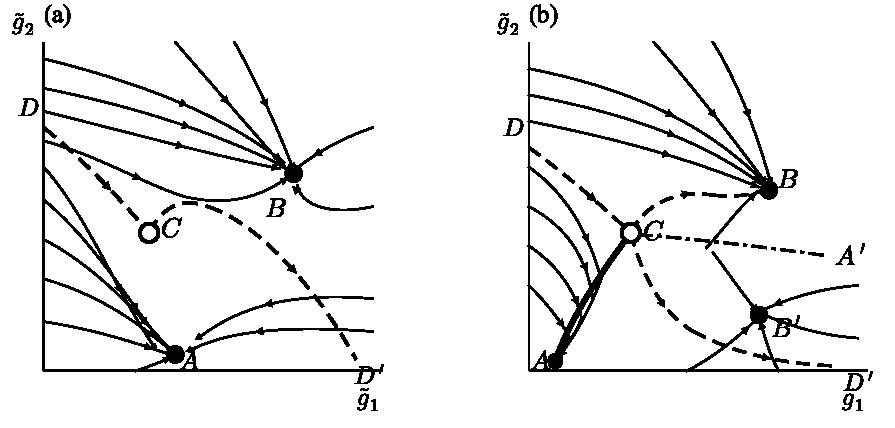
\includegraphics[width=0.72\textwidth]{fig_3.11.pdf}
\caption*{图 3.11\quad (a) A 与 B 是代表两个相的两个稳定不动点。C 是具有一个相关算符/方向的不稳定不动点。A 相与 B 相之间的相变是连续相变。临界点由不稳定不动点 C 描述。(b) 模型 (3.5.3) 的不动点/不动点线结构。CA 是一条稳定不动点线。B 与 B$'$ 是两个稳定不动点。CA、B 与 B$'$ 代表三个相。C 是临界点，代表 A 相（具有代数长程关联）与 B/B$'$ 相（没有长程关联）之间的转变，该转变为 KT 相变。CA$'$ 是一条不稳定不动点线，描述 B 相与 B$'$ 相之间的转变。}
\end{figure}

DCD$'$ 线上方的系统流向另一个不同的不动点，构成另一个普适类。这些系统具有不同的（长距离）普适性质。特别地，它们的衰减指数不同。

普适类与相紧密相关。我们看到，当 $(\tilde{g}_1,\tilde{g}_2)$ 穿过 DCD$'$ 线时，系统的长距离行为与长波涨落突然改变。结果，系统的自由能在 DCD$'$ 线上具有奇异性。因此，DCD$'$ 线是分隔两个相的一条相变线。在这幅图像之下，我们可以说 DCD$'$ 线下方的系统构成一个相，DCD$'$ 线上方的系统构成另一个相。相与普适类在这里意味着同一件事。

让我们从正好位于不动点 A 上的系统出发。我们加上一些微扰，使耦合常数 $(\tilde{g}_1,\tilde{g}_2)$ 偏离 $(\tilde{g}_1(A),\tilde{g}_2(A))$。当 $(\tilde{g}_1,\tilde{g}_2)$ 流回 $(\tilde{g}_1(A),\tilde{g}_2(A))$ 时，微扰在长距离下流向零。因此，这些微扰是不相关微扰。由于稳定不动点周围的所有微扰都流向零，\emph{稳定不动点处的有效理论不含任何相关或边际微扰}。

现在让我们考虑相变点（即临界点）的长距离性质。如果我们从 DCD$'$ 线上的任何位置出发，就可以看到系统流向不动点 C。因此，临界点的长距离行为由不稳定不动点 C 描述。这里我们再次看到普适性：无论从何处穿过相变线，相变点的长距离行为总是相同的。

不动点 C 有一个（且仅有一个）不稳定方向。该方向上的微扰将流离这个不动点。因此，C 的不动点理论有且仅有一个相关微扰。一般地，\emph{描述两相之间相变的临界点有且仅有一个相关微扰}。如果一个不稳定不动点有两个相关微扰，那么该不动点将描述一个三临界点（tri-critical point）。

模型 (3.5.3) 含有一个边际微扰。它的流图更为复杂。（见图 3.11(b)，其中 $(\tilde{g}_1,\tilde{g}_2)$ 对应于 $(\tilde{\eta},\tilde{g})$。）系统有三个相。DCD$'$ 线下方的相由稳定不动点线 AC 控制。这个相具有代数长程关联。代数长程关联的指数依赖于在 AC 线上的位置。DCA$'$ 线上方的相由稳定不动点 B 控制。它没有长程关联，比方说，由 $\langle\cos(\theta)\rangle < 0$ 刻画。D$'$CA$'$ 线右边的相由稳定不动点 B$'$ 控制。它也没有长程关联，由 $\langle\cos(\theta)\rangle > 0$ 刻画。AC 相与 B 相（或 B$'$ 相）之间的相变由不稳定不动点 C 控制，而 B 相与 B$'$ 相之间的相变由不稳定不动点线 CA$'$ 控制。临界指数依赖于在 CA$'$ 线上的位置。

从上面两个简单的例子我们看到，从一个系统的 RG 流图，我们能学到许多关于相与相变的知识。在 3.3.2 节中，我们从对称性破缺的观点讨论了相与相变。本节中我们看到，相与相变也可以基于 RG 图像来理解。这里我想指出，RG 图像（尽管不那么具体）比对称性破缺图像更为基本。对称性破缺图像假定图 3.11(a) 中的两个稳定不动点具有不同的对称性，并且相变线 DCD$'$ 是一条对称性破缺的相变线。这幅对称性破缺图像并不总是正确的。我们可以构造出显式的例子，其中不动点 A 与 B 具有相同的对称性，而相变线 DCD$'$ 不改变任何对称性（Coleman and Weinberg, 1973; Halperin et al., 1974; Fradkin and Shenker, 1979; Wen and Wu, 1993; Senthil et al., 1999; Read and Green, 2000; Wen, 2000）。

\section{玻色超流到莫特绝缘体的转变}

\begin{keypoints}
\item 贝里相项（式 (3.3.20) 中的全导数项 $-\rho_0\partial_t\theta$）在量子 XY 模型中是重要的。它定性地改变了涡旋的性质。
\end{keypoints}

在 $1+1$ 维和零温下，量子玻色超流在低能下同样由一个 XY 模型 (3.3.10) 描述。在虚时中，如果我们取 $v = 1$，量子 XY 模型就与上一节中研究的二维 XY 模型完全相同。虚时 XY 模型中的涡旋对应于可以改变量子系统动力学的隧穿过程。根据 3.4 节得到的结果，看起来当
\begin{equation*}
\chi v < 2/\pi
\end{equation*}
时，瞬子将破坏长程序，使所有关联在空间与时间两个方向上都变成短程的。这意味着瞬子将为所有激发打开一个能隙。上述结论显然是错误的。自由空间中的玻色系统总是可压缩的，它至少含有来自密度波的无能隙模式。

上述论证中的错误相当微妙。为了理解这个错误，我们需要先讨论玻色超流的激发谱。玻色超流中有两类低能激发：对应于声波的局域激发，以及对应于玻色子总数和伽利略助推（Galileo boost）的整体激发。让我们用自由玻色系统作例子，来说明这两类激发。自由玻色系统的基态为 $|k_1,\ldots,k_N\rangle = |0,\ldots,0\rangle$。局域激发通过把若干个 $k$ 改变为某些非零值而产生。低能下，$\sum_i |k_i| \ll \sqrt{\rho}$。整体激发通过往 $k = 0$ 态上添加（或移除）几个玻色子、或者把所有 $k_i$ 平移相同的量而产生。后者称为伽利略助推。对于相互作用玻色系统，伽利略助推可以通过把玻色子的边界条件从 $0$ 扭转到 $2\pi$ 或 $2\pi\times$ 整数来实现，即把常数 $\varphi(x) = \varphi_0$ 改为 $\varphi(x) = \mathrm{e}^{\mathrm{i}2\pi nx/L}\varphi_0$。

让我们考虑处于超流态的相互作用 $N$ 玻色子系统的能级。低能、小动量的激发由声波给出。这些激发的能级如图 3.12(a) 所示。伽利略助推只涉及质心运动。最小的伽利略助推对应于把所有 $k_i$ 平移 $2\pi/L$，其中 $L$ 是系统的线性尺寸。这样的伽利略助推给出一个动量为 $K_1 = 2\pi N/L = 2\pi\rho$、能量为 $E_1 = K_1^2/2mN$ 的激发。我们看到，伽利略助推能量极低但动量很大。因此，伽利略助推不能由声波产生。由 $2\pi n/L$ 的平移所产生的更一般的伽利略助推，具有动量 $K_n = 2\pi nN/L = 2\pi n\rho$ 和能量 $E_n = K_n^2/2mN$。这样，相互作用 $N$ 玻色子系统的低能能级就如图 3.12(b) 所示。$k = K_n$ 附近的能级由第 $n$ 个伽利略助推加上声波给出。

\begin{figure}[H]
\centering
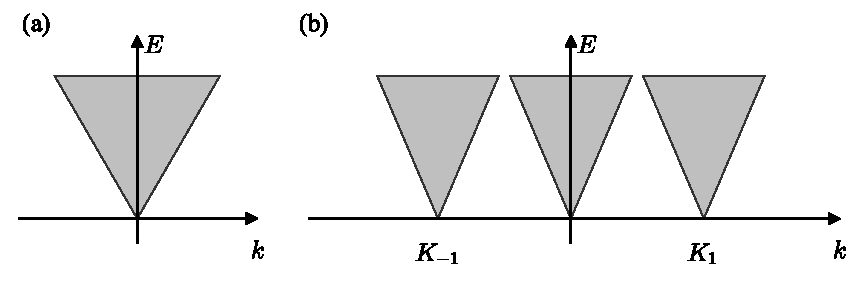
\includegraphics[width=0.72\textwidth]{fig_3.12.pdf}
\caption*{图 3.12\quad $(1+1)$ 维相互作用玻色子的能级，(a) $k \sim 0$，(b) 大 $k$。}
\end{figure}

现在的问题是：超流的低能 XY 模型，即
\begin{equation*}
L_{XY} = \frac{\chi}{2}\dot{\theta}^2 - \frac{\rho}{2m}(\partial_x\theta)^2\tag{3.6.1}
\end{equation*}
能否重现上述谱？让我们展开
\begin{equation*}
\theta(x,t) = \theta_0(t) + n\frac{2\pi x}{L} + \sum_{k\neq 0}\theta_k L^{-1/2}\,\mathrm{e}^{\mathrm{i}kx}
\end{equation*}
第二项描述了当 $x$ 从 $x = 0$ 走到 $x = L$ 时，$\mathrm{e}^{\mathrm{i}\theta(x)}$ 绕零点的缠绕。作用量可以改写为
\begin{equation*}
S_{XY} = \frac{\chi L}{2}\dot{\theta}_0^2 - \frac{K_n^2}{2mN} + \sum_{k>0}\Big[\chi\dot{\theta}_k^\dagger\dot{\theta}_k - \frac{\rho k^2}{2m}\theta_k^\dagger\theta_k\Big]
\end{equation*}
我们看到，$(\theta_k,\theta_{-k})$ 描述一个二维振子，它对应于声波模式。由 3.3.7 节我们看到，$\dot{\theta}_0$ 描述玻色子数涨落，这里将其忽略。现在清楚了，缠绕项 $n\frac{2\pi x}{L}$ 描述一个伽利略助推。这是因为伽利略助推把玻色子场的边界条件从 $\varphi(L) = \varphi(0)$ 扭转到 $\varphi(L) = \mathrm{e}^{\mathrm{i}2\pi n}\varphi(0)$，从而把 $\theta(x) = 0$ 变为 $\theta(x) = 2\pi nx/L$。$\theta$ 场的缠绕与伽利略助推之间的这种关系，也与缠绕所产生的能量 $\frac{K_n^2}{2mN}$ 相一致。

$(1+1)$ 维超流体中 $(x,t)$ 处的一个涡旋，对应于一个算符 $O_v(x,t)$。上述分析表明，算符 $O_v(x,t)$ 把 $k = 0$ 附近的态映射到 $k = 2\pi\rho$ 附近的态。这是因为涡旋把 $\theta(x) = 0$ 变为 $\theta(x) = \frac{2\pi x}{L}$。这样，涡旋就产生了一个伽利略助推。在虚时中，含涡旋的配分函数应具有如下形式
\begin{equation*}
Z = Z_0\sum_n \frac{1}{n!n!}\int\prod_{i=1}^{2n}\mathrm{d}^2\pmb{r}_i\;K^{2n}\,\mathrm{e}^{\mathrm{i}2\pi\rho\sum_j q_j x_j}\,\mathrm{e}^{\sum_{i<j}^{2n} q_iq_j 2\pi\eta\ln\frac{|x_i - x_j|}{l}}
\end{equation*}
其中 $Z_0$ 是没有涡旋时的配分函数。额外的相位项 $\mathrm{e}^{\mathrm{i}2\pi\rho\sum_j q_j x_j}$ 反映了涡旋所携带的大动量。由于这个相位项，涡旋与反涡旋必须成对运动以相互抵消相位，才能有大的贡献。因此，相位项把涡旋与反涡旋禁闭在一起，“库仑”气体没有等离子体相。于是，即使把涡旋包括进来，玻色系统对任何 $\chi$ 与 $v$ 的取值都处于超流相。

然而，如果我们加入一个周期等于平均玻色子间距 $a = 1/\rho$ 的弱周期势，相位项就可以与周期势发生干涉，平均而言变成一个常数。现在我们可以在临界值 $\chi v = 2/\pi$ 处得到 KT 相变。$(1+1)$ 维相互作用玻色子在弱周期势中的相图绘于图 3.13。对于 $\chi v > 2/\pi$，玻色子形成具有代数长程序和无能隙声波模式的导电态。对于 $\chi v < 2/\pi$，所有激发都将具有有限的能隙，玻色子形成一种绝缘体，称为莫特绝缘体（Mott insulator），因为其绝缘性质来源于相互作用而非能带。大势极限下的莫特绝缘体很容易理解：在该极限下，基态在每个势阱中有一个玻色子；把一个玻色子移到另一个势阱，会由于玻色子之间的排斥而耗费有限的能量（见图 3.14）。

\begin{figure}[H]
\centering
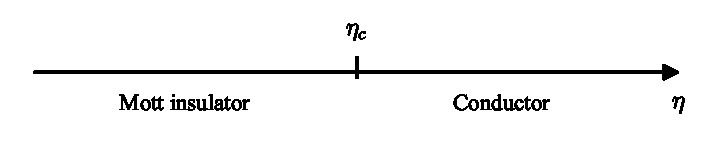
\includegraphics[width=0.72\textwidth]{fig_3.13.pdf}
\caption*{图 3.13\quad $(1+1)$ 维相互作用玻色子在弱周期势中的相图。这里 $\eta = \chi v$，$\eta_c = 2/\pi$。}
\end{figure}

\begin{figure}[H]
\centering
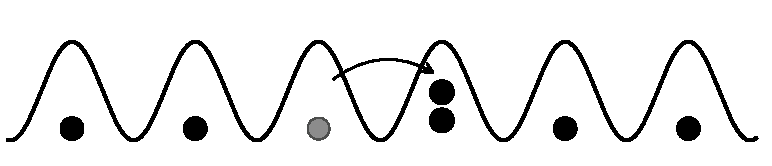
\includegraphics[width=0.72\textwidth]{fig_3.14.pdf}
\caption*{图 3.14\quad 强周期势中 $(1+1)$ 维相互作用玻色子的莫特绝缘体。}
\end{figure}

对涡旋的上述理解也使我们能够计算低能和\emph{大}动量下的密度关联。让我们考虑密度关联函数的谱展开：

% ------------------------------------------------------------
% 块边界备注：
%   起点：书页 111（p126）末行为无编号有效作用量（见本文件顶部注释），
%   本块以 %JOIN% 续书页 112 顶部残句 "where K(x) = n²⟨δθ(x)δθ(0)⟩.
%   We note that the last term can be rewritten as"，与 ch3_d 末式无缝缝合。
%   终点：书页 122（p137）末句 "Let us consider the spectral expansion"
%   跨页延续到书页 123（p138）顶部 "of the density correlation function:"。
%   按 assemble.py 约定，该残句译文（"密度关联函数的谱展开："）应由 ch3_f
%   放入其 %--E-TAIL-- 区（或在其正文开头以 %JOIN% 续译），装配后正好接在
%   本块末尾"让我们考虑"之后；ch3_f 请勿重复翻译，其正文请从 p138 顶部的
%   谱展开无编号式起译。
%   本块含：§3.5.4 末段（自书页 112 顶部续起）、§3.5.5、§3.5.6、§3.5.7 三个
%   \subsection、问题 3.5.2 与 3.5.3、§3.6 的 \section 及其开头（至书页 122 末）。
%   带编号公式 8 个：式 (3.5.8)–(3.5.14)、(3.6.1)；图 3.10–3.14 共 5 个 %FIG；
%   脚注 1 条（原书脚注 23）。
% ------------------------------------------------------------
% 新增术语（ch3_e，待并入术语表"新增术语"区）：
%   running coupling constant 跑动耦合常数；
%   fixed-point theory 不动点理论；attractive fixed point 吸引不动点；
%   unstable fixed point / fixed line 不稳定不动点 / 不动点线；
%   stable fixed line 稳定不动点线；
%   marginal perturbation / operator / coupling constant 边际微扰 / 边际算符 / 边际耦合常数；
%   exact marginal operator 严格边际算符；
%   universality class 普适类；universal properties 普适性质；principle of universality 普适性原理；
%   tri-critical point 三临界点；dynamical symmetry restoration 动力学对称性恢复；
%   Galileo boost 伽利略助推；winding 缠绕；
%   "Coulomb" gas "库仑"气体；plasma phase 等离子体相；
%   conducting state 导电态；potential well 势阱；periodic potential 周期势；
%   local / global excitation 局域激发 / 整体激发；compressible 可压缩的；
%   （备查，ch3_d 范围：Z_n clock model Z_n 时钟模型；compact / non-compact
%   clock model 紧致 / 非紧致时钟模型；background-field RG approach 背景场 RG 方法；
%   Ginzburg–Landau theory Ginzburg–Landau 理论）
% ------------------------------------------------------------

% 边界备注：
%   起点JOIN——书页 123 顶部 "of the density correlation function:" 是书页 122 末句
%   "Let us consider the spectral expansion of the density correlation function:" 的后半句；
%   完整引导句（"让我们考虑密度关联函数的谱展开："）应由上一块的 E-TAIL 收入，
%   本块正文以 %JOIN% 起头，直接从其后的谱展开公式开始。
%   终点——书页 133 止于式 v_c = Min(ε(k)/|k|)，句意完结；书页 134 顶部为图 3.15 与
%   新段落 "It is interesting to see that ..."，属下一块，本块自然结束，无 TAIL。
%   本块范围内无插图（图 3.12–3.14 在书页 121–122，图 3.15 在书页 134），
%   正文引用图 3.1、图 3.15(a)(b)；脚注共 1 处（原书脚注 24）。

%JOIN%
\begin{align*}
\langle\rho(t,x)\rho(0,0)\rangle&=\frac{\langle0|\rho(x)U(t,0)\rho(0)|0\rangle}{\langle0|U(t,0)|0\rangle}\\
&=\sum_{n,k}\langle0|\rho(x)|n,k\rangle\langle n,k|\rho(0)|0\rangle\,\mathrm{e}^{\mathrm{i}kx-\mathrm{i}\epsilon_{n,k}t}
\end{align*}
其中态 $|n,k\rangle$ 具有能量 $\epsilon_{n,k}$ 和动量 $k$。我们还假定了基态 $|0\rangle$ 的能量为零。由于低能态只出现在 $K_i$ 附近，在低能下我们可以把上述求和重新分组如下：
\begin{equation*}
\langle\rho(t,x)\rho(0,0)\rangle=\sum_{n,|\delta k|\ll K_1,i}\langle0|\rho(x)|n,\delta k,i\rangle\langle n,\delta k,i|\rho(0)|0\rangle\,\mathrm{e}^{\mathrm{i}(\delta k+K_i)x-\mathrm{i}\epsilon_{n,\delta k,i}t}
\end{equation*}
其中态 $|n,\delta k,i\rangle$ 具有能量 $\epsilon_{n,\delta k,i}$ 和动量 $\delta k+K_i$。我们看到，大动量处的密度关联，比如 $k\sim K_i$ 处的密度关联，是由矩阵元 $\langle n,\delta k,i|\rho(0)|0\rangle$ 产生的。我们知道，涡旋算符 $O_v^i$（当 $i<0$ 时 $O_v^i\equiv(O_v^\dagger)^{-i}$）把 $k=0$ 附近的低能态映射到 $k=K_i$ 附近的低能态。于是这里我们作如下大胆的假设：
\begin{equation*}
\langle n,\delta k,i|\rho(t,x)|0\rangle=C_i\langle n,\delta k,i|O_v^i(t,x)|0\rangle
\end{equation*}
低能密度算符现在可以推广为
\begin{equation*}
\rho(t,x)=\rho_0-\chi\dot{\theta}(t,x)+\sum_n C_nO_v^n
\end{equation*}
旧结果 $\rho(t,x)=\rho_0-\chi\dot{\theta}(t,x)$ 只描写低能长波长密度涨落，新结果则描写低能全波长密度涨落。我们发现关联函数具有如下形式：
\begin{align*}
\langle\rho(t,x)\rho(0,0)\rangle
&=\rho_0^2-\frac{\chi v}{4\pi}\left(\frac{1}{(x-vt)^2}+\frac{1}{(x+vt)^2}\right)+\sum_n|C_n|^2\mathrm{e}^{\mathrm{i}K_nx}\left(\frac{l^2}{x^2-v^2t^2}\right)^{n^2\pi\chi v}\\
&=\rho_0^2-\left(\frac{\chi v/4\pi}{(x-vt)^2}+\frac{\chi v/4\pi}{(x+vt)^2}\right)+\sum_n|C_n|^2\mathrm{e}^{\mathrm{i}K_nx}\left(\frac{l^2\mathrm{e}^{-\mathrm{i}\pi\Theta(v^2t^2-x^2)}}{|x^2-v^2t^2|}\right)^{n^2\pi\chi v}\tag{3.6.2}
\end{align*}
其中 $l$ 是短距离截断。注意，虚时中的关联 $\langle O_v^\dagger(x,t)O_v(0,0)\rangle$ 由 $\mathrm{e}^{-V}$ 给出，其中 $V$ 是涡旋/反涡旋对之间的势。实时关联则由解析延拓得到。

\subsection*{问题 3.6.1}

证明式 (3.6.2)。

\subsection*{问题 3.6.2}

有限动量下的响应率。
\begin{enumerate}
\item 设玻色子感受到一个弱势 $V(x)$，该势引起密度改变 $\delta\rho$。试把 $\delta\rho_k=\chi(k)V_k$ 中的有限动量响应率 $\chi(k)$ 用频率--动量空间中的密度关联函数表示出来。
\item 求出使响应率 $\chi(K_n)$ 发散的 $\chi$ 与 $v$ 的取值。（提示：先在虚时中做计算可能会容易一些。）
\item 如果我们开启一个周期 $a=\rho^{-1}/n$（$n$ 为整数）的弱周期势，那么对哪些 $\chi$ 与 $v$ 的取值，玻色子形成莫特绝缘体？
\end{enumerate}

\section{超流与超导}

\subsection{与规范场的耦合和守恒流}

\begin{keypoints}
\item 具有整体 $U(1)$ 对称性的理论包含一个守恒荷。
\item 具有整体 $U(1)$ 对称性的理论可以与 $U(1)$ 规范场耦合。电磁矢量势就是一个 $U(1)$ 规范场。
\end{keypoints}

带电玻色子系统会与电磁规范场耦合。当电磁场不为零时，带电玻色子系统的拉格朗日量需要修改。这里的问题是：我们如何找到修改后的拉格朗日量？我们知道，玻色子拉格朗日量
\begin{equation*}
L(\varphi)=\mathrm{i}\frac{1}{2}(\varphi^*\partial_t\varphi-\varphi\partial_t\varphi^*)-\frac{1}{2m}\partial_{\pmb{x}}\varphi^*\partial_{\pmb{x}}\varphi+\mu|\varphi|^2-\frac{V_0}{2}|\varphi|^4 \tag{3.7.1}
\end{equation*}
在整体 $U(1)$ 变换
\begin{equation*}
\varphi\rightarrow\mathrm{e}^{\mathrm{i}f}\varphi
\end{equation*}
下不变，即 $L(\mathrm{e}^{\mathrm{i}f}\varphi)=L(\varphi)$。但它在一个局域 $U(1)$ 变换
\begin{equation*}
\varphi(\pmb{x},t)\rightarrow\mathrm{e}^{\mathrm{i}f(\pmb{x},t)}\varphi(\pmb{x},t)
\end{equation*}
下并非不变。我们有
\begin{align*}
L(\mathrm{e}^{\mathrm{i}f(\pmb{x},t)}\varphi)&=\mathrm{i}\frac{1}{2}\big(\varphi^*(\partial_0+\mathrm{i}\partial_0f)\varphi-\varphi(\partial_0-\mathrm{i}\partial_0f)\varphi^*\big)\\
&\quad-\frac{1}{2m}\big|(\partial_i+\mathrm{i}\partial_if)\varphi\big|^2+\mu|\varphi|^2-\frac{V_0}{2}|\varphi|^4 \tag{3.7.2}
\end{align*}
其中下标 0 标记时间方向，下标 $i=1,\dots,d$ 标记空间方向。我们将用希腊字母 $\mu,\nu$ 等标记时空方向。例如，$x^\mu$ 代表时空坐标。玻色子与电磁规范场的耦合现在只需把 $\partial_\mu f$ 换成 $A_\mu$ 便可得到：
\begin{align*}
L(\varphi,A_\mu)&=\mathrm{i}\frac{1}{2}\big(\varphi^*(\partial_0+\mathrm{i}A_0)\varphi-\varphi(\partial_0-\mathrm{i}A_0)\varphi^*\big)\\
&\quad-\frac{1}{2m}\big|(\partial_i+\mathrm{i}A_i)\varphi\big|^2+\mu|\varphi|^2-\frac{V_0}{2}|\varphi|^4 \tag{3.7.3}
\end{align*}
所得的拉格朗日量有一个很好的性质：它是规范不变的：
\begin{gather*}
\varphi\rightarrow\tilde{\varphi}=\mathrm{e}^{\mathrm{i}f(\pmb{x},t)}\varphi\\
A_\mu\rightarrow\tilde{A}_\mu=A_\mu-\partial_\mu f\\
L(\varphi,A_\mu)\rightarrow L(\tilde{\varphi},\tilde{A}_\mu)=L(\varphi,A_\mu) \tag{3.7.4}
\end{gather*}
上述构造并不包含多少物理，它只是得到规范不变拉格朗日量的一个技巧。这一技巧给出最简单的拉格朗日量，称为最小耦合（minimal coupling）。我们也可以写出别的规范不变拉格朗日量，例如把 $\partial_\mu f$ 换成 $A_\mu+g\partial_\nu F_{\nu\mu}$，其中 $F_{\mu\nu}=\partial_\mu A_\nu-\partial_\nu A_\mu$ 是 $A_\mu$ 的场强。注意 $F_{\mu\nu}$ 在规范变换下不变。

式 (3.7.3) 只描写荷场 $\varphi$ 与规范场 $A_\mu$ 之间的耦合。同时描写 $\varphi$ 与 $A_\mu$ 二者动力学的完整规范不变拉格朗日量为
\begin{align*}
L(\varphi,A_\mu)&=\mathrm{i}\frac{1}{2}\big(\varphi^*(\partial_0+\mathrm{i}A_0)\varphi-\varphi(\partial_0-\mathrm{i}A_0)\varphi^*\big)-\frac{1}{2m}\big|(\partial_i+\mathrm{i}A_i)\varphi\big|^2\\
&\quad+\mu|\varphi|^2-\frac{V_0}{2}|\varphi|^4+\frac{1}{8\pi e^2}\left(\frac{1}{c}\pmb{E}^2-c\pmb{B}^2\right) \tag{3.7.5}
\end{align*}
其中 $c$ 是光速，而
\begin{equation*}
E_i=\partial_0A_i-\partial_iA_0=F_{0i},\qquad B_i=\epsilon_{ijk}\partial_jA_k=\frac{1}{2}\epsilon_{ijk}F_{jk}
\end{equation*}
分别是 $U(1)$ 规范理论的电场和磁场。

我们知道，具有整体 $U(1)$ 对称性的模型有一个守恒荷。借助规范场可以容易地证明这一点。规范化后的作用量是规范不变的：
\begin{equation*}
S(\varphi,A_\mu)=S(\mathrm{e}^{\mathrm{i}f(\pmb{x},t)}\varphi,A_\mu-\partial_\mu f)
\end{equation*}
设 $\varphi_c(\pmb{x},t)$ 是经典运动方程的一个解，那么
\begin{equation*}
S(\mathrm{e}^{\mathrm{i}f(\pmb{x},t)}\varphi_c,A_\mu)=S(\varphi_c,A_\mu)+O(f^2)
\end{equation*}
因此
\begin{align*}
S(\varphi_c,A_\mu)&=S(\varphi_c,A_\mu-\partial_\mu f)+O(f^2)\\
&=S(\varphi_c,A_\mu)+\int\mathrm{d}^d\pmb{x}\,\mathrm{d}t\,\partial_\mu f\,J^\mu(\varphi_c,A_\mu)+O(f^2)
\end{align*}
其中 $J^\mu$ 是流
\begin{equation*}
J^\mu(\varphi,A_\mu)\equiv-\partial_{A_\mu}L(\varphi,A_\mu)
\end{equation*}
我们看到，如果 $\varphi(\pmb{x},t)$ 满足经典运动方程，则对任意 $f$ 都有 $\int\mathrm{d}^d\pmb{x}\,\mathrm{d}t\,\partial_\mu f\,J^\mu(\varphi_c,A_\mu)=0$，于是流 $J^\mu(\varphi_c,A_\mu)$ 守恒：
\begin{equation*}
\partial_\mu J^\mu(\varphi_c,A_\mu)=\partial_t\rho+\partial_iJ^i=0
\end{equation*}
其中 $\rho=J^0$ 是密度，$J^i$ 是流。当然，上述结果对 $A_\mu$ 场为零的情形同样成立，我们有 $\partial_\mu J^\mu(\varphi_c)=0$，这正是中性系统的流守恒。

对我们的玻色子系统，求得守恒流为
\begin{gather*}
J^0=\rho=\varphi^*\varphi\\
J^i=-\frac{\mathrm{i}}{2m}\big[\varphi^*(\partial_i\varphi)-(\partial_i\varphi^*)\varphi\big]+A_i|\varphi|^2
\end{gather*}
有意思的是，我们玻色子系统中的流依赖于规范势。

\subsection*{问题 3.7.1}

考虑一个与规范场耦合的格点玻色子系统：
\begin{equation*}
L=\mathrm{i}\frac{1}{2}\sum_i\big(\varphi_i^*(\partial_0+\mathrm{i}A_0(i))\varphi_i-\varphi_i(\partial_0-\mathrm{i}A_0(i))\varphi_i^*\big)+\sum_{\langle ij\rangle}\big(t_{ij}\varphi_j^*\varphi_i\,\mathrm{e}^{-\mathrm{i}a_{ij}}+\mathrm{h.c.}\big)
\end{equation*}
其中求和遍及所有对 $\langle ij\rangle$，$a_{ij}$ 是规范场 $a_{ij}=\int_i^j\mathrm{d}\pmb{x}\cdot\pmb{A}$。
\begin{enumerate}
\item 证明 $L$ 在格点规范变换（lattice gauge transformation）
\begin{equation*}
\varphi_i\rightarrow\mathrm{e}^{\mathrm{i}f_i(t)}\varphi_i,\qquad A_0(i)\rightarrow A_0(i)-\partial_0f_i,\qquad a_{ij}\rightarrow a_{ij}-f_j+f_i
\end{equation*}
下不变。
\item 求 $\varphi_i(t)$ 的运动方程。
\item 计算密度的时间导数，即 $\partial_0\varphi_i^*\varphi_i$。证明可以引入一个定义在链上的流 $J_{ij}$，并恢复格点流守恒关系
\begin{equation*}
\partial_0\varphi_i^*\varphi_i+\sum_jJ_{ij}=0
\end{equation*}
\item 证明 $J_{ij}$ 可以表示为 $-\partial L/\partial a_{ij}$。
\end{enumerate}

\subsection{流关联函数与电磁响应}

\begin{keypoints}
\item 流守恒对流关联施加了约束。许多重要的物理量，如压缩率和电导率（conductivity），都由流关联决定。
\item 要得到正确的响应，重要的是按正确的次序取 $\pmb{k}\to0$ 与 $\omega\to0$ 这两个极限。
\end{keypoints}

现在让我们计算系统对外加规范势的响应。我们想看看规范势 $A_\mu$ 能产生多大的流 $J^\mu$。按下式引入 $j^\mu$：
\begin{equation*}
j^0=\rho,\qquad j^i=-\frac{\mathrm{i}}{2m}\big[\varphi^*(\partial_i\varphi)-(\partial_i\varphi^*)\varphi\big]
\end{equation*}
我们看到拉格朗日量具有形式
\begin{equation*}
L(\varphi,A_\mu)=L(\varphi)-A_0j^0-A_ij^i-\frac{1}{2m}(A^i)^2\rho
\end{equation*}
利用线性响应理论计算 $\langle j^\mu(\pmb{x},t)\rangle$ 到 $A_\mu$ 的领头阶，我们得到流 $J^\mu\equiv-\partial_{A_\mu}L$：
\begin{equation*}
\langle J^\mu(\pmb{x},t)\rangle=\langle j^\mu(\pmb{x},t)\rangle+(1-\delta^{\mu0})A^\mu\rho=\int\mathrm{d}^d\pmb{x}\,\mathrm{d}t\,\Pi^{\mu\nu}(\pmb{x},t;\pmb{x}',t')A_\nu(\pmb{x}',t')
\end{equation*}
其中响应函数为
\begin{align*}
\Pi^{00}(\pmb{x},t;\pmb{x}',t')&=-\mathrm{i}\Theta(t-t')\,\big\langle[\rho(\pmb{x},t),\rho(\pmb{x}',t')]\big\rangle\\
\Pi^{0i}(\pmb{x},t;\pmb{x}',t')&=-\mathrm{i}\Theta(t-t')\,\big\langle[\rho(\pmb{x},t),j^i(\pmb{x}',t')]\big\rangle\\
\Pi^{i0}(\pmb{x},t;\pmb{x}',t')&=-\mathrm{i}\Theta(t-t')\,\big\langle[j^i(\pmb{x},t),\rho(\pmb{x}',t')]\big\rangle\\
\Pi^{ij}(\pmb{x},t;\pmb{x}',t')&=-\mathrm{i}\Theta(t-t')\,\big\langle[j^i(\pmb{x},t),j^j(\pmb{x}',t')]\big\rangle+\delta^{ij}\delta(\pmb{x}-\pmb{x}')\delta(t-t')\frac{\langle\rho\rangle}{m}
\end{align*}
由于流依赖于 $A_i$，我们多出一个接触项（contact term）$\delta^{ij}\delta(\pmb{x}-\pmb{x}')\delta(t-t')\frac{\langle\rho\rangle}{m}$。如果我们引入关联函数
\begin{equation*}
\pi^{\mu\nu}(\pmb{x},t;\pmb{x}',t')=-\mathrm{i}\Theta(t-t')\,\big\langle[j^\mu(\pmb{x},t),j^\nu(\pmb{x}',t')]\big\rangle
\end{equation*}
则
\begin{equation*}
\Pi^{\mu\nu}=\pi^{\mu\nu}+\delta^{\mu\nu}(1-\delta^{0\mu})(1-\delta^{0\nu})\delta(\pmb{x}-\pmb{x}')\delta(t-t')\langle\rho\rangle \tag{3.7.6}
\end{equation*}
上述结果对零温和有限温都成立。我们注意到
\begin{equation*}
\big(\Pi^{\mu\nu}(\pmb{x},t;\pmb{x}',t')\big)^*=\Pi^{\nu\mu}(\pmb{x}',t';\pmb{x},t)
\end{equation*}
或者，在 $\omega$--$\pmb{k}$ 空间中，
\begin{equation*}
\big(\Pi^{\mu\nu}_{(k_\lambda)}\big)^*=\Pi^{\nu\mu}_{(-k_\lambda)}
\end{equation*}
其中 $k_0=\omega$。

由于流守恒，$\Pi^{\mu\nu}$ 的各分量并非完全独立。在 $\omega$--$\pmb{k}$ 空间中，我们有
\begin{equation*}
k_\mu\Pi^{\mu\nu}_{k_\lambda}=0
\end{equation*}
于是，完整的 $\Pi^{\mu\nu}$ 可以由 $\Pi^{ij}$ 按如下方式确定：
\begin{align*}
\Pi^{0i}_{(k_\lambda)}&=\big(\Pi^{i0}_{(-k_\lambda)}\big)^\dagger=-\frac{k_j}{\omega}\Pi^{ji}_{(k_\lambda)}\\
\Pi^{00}_{(k_\lambda)}&=-\frac{k_j}{\omega}\Pi^{0j}_{(k_\lambda)}=\frac{k_ik_j}{\omega^2}\Pi^{ij}_{(k_\lambda)} \tag{3.7.7}
\end{align*}
对于转动不变的系统，我们还可以把 $\Pi^{ij}$ 和 $\pi^{ij}$ 进一步分解成一个纵向分量（longitudinal component）$\Pi^{\parallel}_{(k_\lambda)}$ 和一个横向分量（transverse component）$\Pi^{\perp}_{(k_\lambda)}$：
\begin{align*}
\Pi^{ij}_{(k_\lambda)}&=\frac{k_ik_j}{\pmb{k}^2}\Pi^{\parallel}_{(k_\lambda)}+\Big(\delta_{ij}-\frac{k_ik_j}{\pmb{k}^2}\Big)\Pi^{\perp}_{(k_\lambda)}\\
\pi^{ij}_{(k_\lambda)}&=\frac{k_ik_j}{\pmb{k}^2}\pi^{\parallel}_{(k_\lambda)}+\Big(\delta_{ij}-\frac{k_ik_j}{\pmb{k}^2}\Big)\pi^{\perp}_{(k_\lambda)} \tag{3.7.8}
\end{align*}
式 (3.7.7) 现在可以写成
\begin{equation*}
\Pi^{0i}_{(k_\lambda)}=-k_i\Pi^{\parallel}_{(k_\lambda)},\qquad \Pi^{00}_{(k_\lambda)}=\frac{\pmb{k}^2}{\omega^2}\Pi^{\parallel}_{(k_\lambda)}
\end{equation*}
而式 (3.7.6) 可以写成
\begin{equation*}
\Pi^{\parallel}_{(k_\lambda)}=\pi^{\parallel}_{(k_\lambda)}+\frac{\langle\rho\rangle}{m},\qquad \Pi^{\perp}_{(k_\lambda)}=\pi^{\perp}_{(k_\lambda)}+\frac{\langle\rho\rangle}{m}, \tag{3.7.9}
\end{equation*}
响应函数 $\Pi^{\mu\nu}$ 与许多重要的物理量相关。让我们以金属为例。在 $\omega\to0$ 极限下，我们有
\begin{equation*}
\delta\rho(\pmb{k})=\Pi^{00}_{(0,\pmb{k})}A_0(\pmb{k})
\end{equation*}
注意 $A_0(\pmb{x})$ 正是外加势，而 $-\Pi^{00}_{(0,\pmb{k})}$ 就是（波矢 $\pmb{k}$ 处的）压缩率：
\begin{equation*}
\chi(\pmb{k})=-\Pi^{00}_{(0,\pmb{k})}
\end{equation*}
通常，我们预期 $\Pi^{00}_{(0,\pmb{k})}$ 对所有 $\pmb{k}$ 都有限。于是，在小 $\omega$ 以及 $\omega\ll\pmb{k}$ 的极限下（注意这里我们先取 $\omega\to0$），我们有
\begin{equation*}
\Pi^{\parallel}_{(k_\lambda)}=-\chi(\pmb{k})\frac{\omega^2}{\pmb{k}^2}
\end{equation*}
由式 (3.7.9) 可见，在 $\omega\to0$ 极限下，$\pi^{\parallel}_{(k_\lambda)}$ 必须恰好抵消 $\frac{\langle\rho\rangle}{m}$，才能使 $\Pi^{\parallel}_{(k_\lambda)}$ 像 $\omega^2$ 那样趋于零。

现在让 $\pmb{k}$ 先趋于零。在 $|\pmb{k}|\ll\omega$ 极限下，$-\mathrm{i}\omega A_{i,(\omega,\pmb{k})}$ 是一个近乎均匀的电场，预期它会产生一个方向由 $A_i$ 给出、波矢由 $\pmb{k}$ 给出的流：
\begin{equation*}
J^i(\omega)=\lim_{\pmb{k}\to0}\frac{\Pi^{ij}}{-\mathrm{i}\omega}(-\mathrm{i}\omega)A_{j,(\omega,\pmb{k})}
\end{equation*}
由式 (3.7.8) 我们看到，只有当 $\omega\gg|\pmb{k}|$ 极限下 $\Pi^{\parallel}_{(k_\lambda)}=\Pi^{\perp}_{(k_\lambda)}$ 时，$\pmb{k}\to0$ 的极限才存在。假设情形正是如此，那么我们得到电导率
\begin{equation*}
\sigma(\omega)=\frac{\Pi^{\parallel}_{(\omega,0)}}{-\mathrm{i}\omega}=\frac{\Pi^{\perp}_{(\omega,0)}}{-\mathrm{i}\omega}
\end{equation*}
电导率的实部
\begin{equation*}
\mathrm{Re}\,\sigma(\omega)=-\mathrm{Im}\frac{\Pi^{\parallel}_{(\omega,0)}}{\omega}=-\mathrm{Im}\frac{\Pi^{\perp}_{(\omega,0)}}{\omega}
\end{equation*}
对应于耗散。电导率的虚部给出介电常数
\begin{equation*}
\epsilon(\omega)=-\frac{\mathrm{Im}\,\sigma(\omega)}{\omega}=\mathrm{Re}\frac{\Pi^{\parallel}_{(\omega,0)}}{\omega^2}=\mathrm{Re}\frac{\Pi^{\perp}_{(\omega,0)}}{\omega^2}
\end{equation*}
于是，在 $\omega\gg|\pmb{k}|$ 极限下，我们可以写成
\begin{equation*}
\Pi^{\parallel}_{(\omega,0)}=\Pi^{\perp}_{(\omega,0)}=\mathrm{i}\omega\,\mathrm{Re}\,\sigma(\omega)+\omega^2\epsilon(\omega)
\end{equation*}
我们注意到，极化矢量 $\pmb{P}$ 满足 $\partial_{\pmb{x}}\cdot\pmb{P}=-\delta\rho$，或者（假定 $A_i=0$）
\begin{equation*}
\mathrm{i}k_iP^i=-\delta\rho=-\Pi^{00}A_0=-\frac{\pmb{k}^2}{\omega^2}\Pi^{\parallel}_{(k_\lambda)}A_0=\mathrm{i}\frac{\Pi^{\parallel}_{(k_\lambda)}}{\omega^2}k_iE_i
\end{equation*}
因此
\begin{equation*}
P^i=\frac{\Pi^{\parallel}_{(k_\lambda)}}{\omega^2}E_i
\end{equation*}
我们又看到 $\Pi^{\parallel}_{(k_\lambda)}/\omega^2$ 是介电常数。

我们已经考虑了 $\Pi^{\parallel}$ 和 $\Pi^{\perp}$ 的 $\omega\gg|\pmb{k}|$ 极限，以及 $\Pi^{\parallel}$ 的 $\omega\ll|\pmb{k}|$ 极限。那么 $\Pi^{\perp}$ 的 $\omega\ll|\pmb{k}|$ 极限是什么呢？一个自然的猜测是它对应于磁化率。磁矩密度 $\pmb{M}$ 满足 $\partial_{\pmb{x}}\times\pmb{M}=-\pmb{j}$。于是（假定 $A_0=0$），我们有
\begin{align*}
\mathrm{i}\epsilon^{ijk}k_jM_k&=-j^i=-\Pi^{ij}A_j=-(\delta^{ij}\pmb{k}^2-k^ik^j)A_j\frac{\Pi^{\perp}_{(k_\lambda)}}{\pmb{k}^2}\\
&=+\epsilon^{ij'k'}k_{j'}\epsilon^{k'i'j}k_{i'}A_j\frac{\Pi^{\perp}_{(k_\lambda)}}{\pmb{k}^2}=-\mathrm{i}\epsilon^{ijk}k_jB_k\frac{\Pi^{\perp}_{(k_\lambda)}}{\pmb{k}^2}
\end{align*}
因此
\begin{equation*}
M_i=-\frac{\Pi^{\perp}_{(k_\lambda)}}{k^2}B_i
\end{equation*}
而 $-\Pi^{\perp}_{(k_\lambda)}/k^2$ 就是磁化率。

现在让我们计算玻色子超流体的 $\Pi^{\mu\nu}$。我们从带规范场 (3.7.3) 的玻色子拉格朗日量出发，积掉振幅涨落，得到一个带规范场的 XY 模型。保留到 $(\partial_\mu\theta,A_\mu)$ 的二次阶，我们有
\begin{equation*}
L=\frac{\chi}{2}\big((\partial_0\theta+A_0)^2-v^2(\partial_i\theta+A_i)^2\big) \tag{3.7.10}
\end{equation*}
由此我们看到
\begin{equation*}
j^0=-\chi\partial_0\theta,\qquad j^i=\chi v^2\partial_i\theta
\end{equation*}
因此
\begin{align*}
\pi^{00}&=\chi^2(-\mathrm{i}\omega)(\mathrm{i}\omega)\big\langle\theta_{(\omega,\pmb{k})}\theta_{(-\omega,-\pmb{k})}\big\rangle=\chi\frac{\omega^2}{\omega^2-v^2\pmb{k}^2+\mathrm{i}0^+\mathrm{sgn}(\omega)}\\
\pi^{0i}&=\pi^{i0}=\chi^2(-\mathrm{i}\omega)(-\mathrm{i}k_i)\big\langle\theta_{(\omega,\pmb{k})}\theta_{(-\omega,-\pmb{k})}\big\rangle=-\chi v^2\frac{\omega k_i}{\omega^2-v^2\pmb{k}^2+\mathrm{i}0^+\mathrm{sgn}(\omega)}\\
\pi^{ij}&=\chi^2(\mathrm{i}k_i)(-\mathrm{i}k_j)\big\langle\theta_{(\omega,\pmb{k})}\theta_{(-\omega,-\pmb{k})}\big\rangle=\chi v^4\frac{k_ik_j}{\omega^2-v^2\pmb{k}^2+\mathrm{i}0^+\mathrm{sgn}(\omega)}
\end{align*}
注意，$\mathrm{i}0^+\mathrm{sgn}(\omega)$ 的选择给出的正是响应函数。总的 $\Pi^{\mu\nu}$ 为
\begin{align*}
\Pi^{00}&=\chi\left(\frac{\omega^2}{\omega^2-v^2\pmb{k}^2+\mathrm{i}0^+\mathrm{sgn}(\omega)}-1\right)\\
\Pi^{0i}&=\Pi^{i0}=-\chi v^2\frac{\omega k_i}{\omega^2-v^2\pmb{k}^2+\mathrm{i}0^+\mathrm{sgn}(\omega)}\\
\Pi^{ij}&=\chi v^2\left(\delta_{ij}+v^2\frac{k_ik_j}{\omega^2-v^2\pmb{k}^2+\mathrm{i}0^+\mathrm{sgn}(\omega)}\right)
\end{align*}
而
\begin{gather*}
\Pi^{\parallel}=\chi v^2\left(\frac{v^2k^2}{\omega^2-v^2\pmb{k}^2+\mathrm{i}0^+\mathrm{sgn}(\omega)}+1\right)\\
\Pi^{\perp}=\chi v^2
\end{gather*}
压缩率 $-\Pi^{00}_{(0,\pmb{k})}$ 有限且等于 $\chi$。磁化率 $-\Pi^{\perp}/c\pmb{k}^2$ 在 $\pmb{k}\to0$ 时发散。电导率的实部
\begin{equation*}
\mathrm{Re}\,\sigma(\omega)=-\mathrm{Im}\frac{\Pi^{\parallel}_{(\omega,0)}}{\omega}=\mathrm{Im}\frac{\chi v^2}{\omega+\mathrm{i}0^+}=\pi\frac{\rho}{m}\delta(\omega)
\end{equation*}
在有限频率处为零。

如果我们选取库仑规范（Coulomb gauge）$\partial_{\pmb{x}}\cdot\pmb{A}=0$，那么由 $J^i=\Pi^{ij}A_j$，我们发现流与\emph{规范势}之间的一个简单关系：
\begin{equation*}
\pmb{J}=\Pi^{\perp}\pmb{A}=\frac{\rho}{m}\pmb{A} \tag{3.7.11}
\end{equation*}
这就是著名的伦敦方程（London equation）。超导体的许多新奇性质——如持续电流（persistent current）、迈斯纳效应等——都由它负责。

\subsection{超流性与有限温度效应}

\begin{keypoints}
\item 激发会削弱超流，但无法消灭它。这导致了超流性。
\item 超流只能靠涡旋的隧穿来消灭。
\item 超流的临界速度。
\end{keypoints}

最后，我们准备讨论相互作用玻色子对称性破缺相的超流性质（Landau, 1941）。首先考虑自由空间中的玻色子系统。该玻色子系统在伽利略变换（Galileo transformation）下不变。让我们假定对称性破缺基态之上的激发具有谱 $\epsilon(\pmb{k})$，并忽略激发之间的相互作用。后一假定在低温、激发稀薄时成立。

考察（静止的）基态之上的一个单激发 $(\epsilon,\pmb{k})$。系统的总能量与总动量分别为 $E_{\mathrm{ground}}+\epsilon$ 与 $\pmb{P}=\pmb{k}$。如果我们以速度 $\pmb{v}$ 推动（boost）系统，则系统的总能量与总动量将分别变为 $E=E_{\mathrm{ground}}+\epsilon+\frac{1}{2}Nm\pmb{v}^2+\pmb{v}\cdot\pmb{k}$ 与 $\pmb{P}=\pmb{k}+Nm\pmb{v}$。与被推动基态的能量和动量（即 $E=E_{\mathrm{ground}}+\frac{1}{2}Nm\pmb{v}^2$ 与 $\pmb{P}=Nm\pmb{v}$）相比，我们看到被推动基态之上的激发具有新谱
\begin{equation*}
\epsilon_{\pmb{v}}(\pmb{k})=\epsilon(\pmb{k})+\pmb{v}\cdot\pmb{k}
\end{equation*}
在被推动的超流体中，动量为 $\pmb{k}$ 的激发的占据数由 $n_B(\epsilon(\pmb{k}))$ 给出，其中 $n_B(\epsilon)=1/(\mathrm{e}^{\epsilon/T}-1)$。被推动超流体的能量与动量分别可写为
\begin{gather*}
\tilde{E}=E_{\mathrm{ground}}+\sum_{\pmb{k}}\epsilon_{\pmb{v}}(\pmb{k})n_B(\epsilon(\pmb{k}))+\frac{1}{2}Nm\pmb{v}^2\\
\tilde{\pmb{P}}=\sum_{\pmb{k}}\pmb{k}\,n_B(\epsilon(\pmb{k}))+Nm\pmb{v}=Nm\pmb{v}
\end{gather*}
在平衡态中，激发的占据数应为 $n_B(\epsilon_{\pmb{v}}(\pmb{k}))$。我们看到，被推动的超流体并不处于平衡态。如果我们让系统通过重新分配激发而弛豫到实验室系中的平衡态，那么能量与动量将分别变为
\begin{gather*}
E_{\pmb{v}}=E_{\mathrm{ground}}+\sum_{\pmb{k}}\epsilon_{\pmb{v}}(\pmb{k})n_B(\epsilon_{\pmb{v}}(\pmb{k}))+\frac{1}{2}Nm\pmb{v}^2\\
\pmb{P}_{\pmb{v}}=\sum_{\pmb{k}}\pmb{k}\,n_B(\epsilon_{\pmb{v}}(\pmb{k}))+Nm\pmb{v}
\end{gather*}
对于小的 $\pmb{v}$，上式可重写为\footnote{$\pmb{P}_{\pmb{v}}$ 的结果很容易看出。为得到 $E_{\pmb{v}}$，我们注意到
\begin{align*}
E_{\pmb{v}}&=E_{\mathrm{ground}}+\sum_{\pmb{k}}\epsilon(\pmb{k})n_B(\epsilon(\pmb{k}))+\sum_{\pmb{k}}(\pmb{v}\cdot\pmb{k})^2\big[n_B'(\epsilon(\pmb{k}))+\tfrac{1}{2}\epsilon(\pmb{k})n_B''(\epsilon(\pmb{k}))\big]+\frac{1}{2}Nm\pmb{v}^2\\
&=E_0-\frac{1}{2}\mathcal{V}m\rho_n\pmb{v}^2+\frac{1}{2d}\pmb{v}^2\sum_{\pmb{k}}\pmb{k}^2\frac{\mathrm{d}}{\mathrm{d}\epsilon(\pmb{k})}\big[\epsilon(\pmb{k})n_B'(\epsilon(\pmb{k}))\big]+\frac{1}{2}Nm\pmb{v}^2
\end{align*}}
\begin{align*}
E_{\pmb{v}}&=E_0+\frac{1}{2}\big[Nm-\mathcal{V}(\rho_nm+\delta\rho_nm)\big]\pmb{v}^2\\
\pmb{P}_{\pmb{v}}&=(Nm-\mathcal{V}\rho_nm)\pmb{v} \tag{3.7.12}
\end{align*}
其中
\begin{equation*}
\rho_n=-\frac{1}{md}\int\frac{\mathrm{d}^d\pmb{k}}{(2\pi)^d}\,\pmb{k}^2n_B'(\epsilon(\pmb{k})) \tag{3.7.13}
\end{equation*}
\begin{equation*}
\delta\rho_n=-\frac{1}{md}\int\frac{\mathrm{d}^d\pmb{k}}{(2\pi)^d}\,\pmb{k}^2\frac{\mathrm{d}}{\mathrm{d}\epsilon(\pmb{k})}\big(\epsilon(\pmb{k})n_B'(\epsilon(\pmb{k}))\big) \tag{3.7.14}
\end{equation*}
如果对小 $\pmb{k}$ 有 $\epsilon(\pmb{k})\propto|\pmb{k}|$，则对小 $T$ 有 $\rho_n\propto T^{d+1}$。

这里我们看到对称性破缺相的一个惊人性质：在我们让激发弛豫到平衡态之后，系统的总动量 $\pmb{P}_{\pmb{v}}$ 并不弛豫到零。平衡态中玻色子永远运动下去。正是这一性质让对称性破缺相得到了“超流体”这个名字。为了更好地理解这一现象，我们回顾一下：在对称性破缺相中，玻色子场可以写成
\begin{equation*}
\varphi=\varphi_0+\delta\varphi
\end{equation*}
其中 $\varphi_0$ 描写凝聚体，$\delta\varphi$ 描写凝聚体之上的激发。设玻色子处于线度为 $L$、带周期边界条件的盒子中。当我们推动系统时，我们把玻色子边界条件从 $\varphi(L)=\varphi(0)$ 扭转到 $\varphi(L)=\mathrm{e}^{\mathrm{i}mvL}\varphi(0)$。于是，在这一推动下，$\varphi$ 变为 $\mathrm{e}^{\mathrm{i}mvx}\varphi$。在被推动的超流体中，凝聚体被扭转：$\varphi_0\to\mathrm{e}^{\mathrm{i}mvx}\varphi_0$（见图 3.15(a)）。由于周期边界条件，$mvL$ 按 $2\pi\times$ 整数量子化。现在很清楚：由于 $|\varphi_0|$ 固定，我们不可能在不撕裂凝聚体的情况下解除扭转。解除凝聚体的扭转需要把凝聚体 $\varphi_0$ 压到零，这要耗费巨大的能量。更确切地说，解除扭转需要产生一个涡旋，并让这个涡旋一路移动、横穿整个样品（见图 3.15(b)）。因此，解除凝聚体的扭转是一个具有有限能量势垒的隧穿过程。按照这幅图像，我们看到：如果忽略隧穿过程，运动的超流体尽管能量较高，也不能弛豫回基态。我们还学到，超流体并不能真正地永远流动。隧穿会使流动弛豫到零，不过这可能需要非常非常长的时间。超流动性的关键在于无穷大系统中涡旋的无穷大能量代价，而这一无穷大的能量代价来自式 (3.4.2) 中有限的相位劲度（phase rigidity）$\eta\neq0$。

然而，对激发来说，情况就大不相同了。这里 $\delta\varphi$ 在零附近涨落，可以扭转并轻易地改变自己的相位。因此，涨落（即激发）能够通过其与环境的相互作用（这种相互作用可以非常弱）轻易地弛豫到平衡态。

上述讨论暗示了一幅两流体（two-fluid）图像。玻色子超流体包含两个组分：与凝聚体相联系的超流组分，以及与激发相联系的正常流体组分。当玻色子超流体流过管道时，只有超流组分能够无摩擦地流过。摩擦太大时，正常流体组分无法流动。（在稳态下管道内没有压差，正常流体组分便完全无法流动。）当然，超流的速度不能太大。如果 $\pmb{v}$ 太大，实验室系中的激发能量 $\epsilon_{\pmb{v}}(\pmb{k})$ 可能变成负值，这意味着不稳定以及无摩擦流动的终结。因此，临界速度为（见图 3.1）
\begin{equation*}
v_c=\mathrm{Min}\big(\epsilon(\pmb{k})/|\pmb{k}|\big)
\end{equation*}

% ==================================================================
% 新增术语（ch3_f 新增，供术语表追加）：
%   minimal coupling 最小耦合；contact term 接触项；
%   conductivity 电导率；longitudinal/transverse component 纵向分量 / 横向分量；
%   Coulomb gauge 库仑规范；polarization vector 极化矢量；
%   magnetic moment density 磁矩密度；London equation 伦敦方程；
%   Meissner effect 迈斯纳效应；persistent current 持续电流；
%   lattice gauge transformation 格点规范变换；
%   Galileo transformation / Galileo invariance 伽利略变换 / 伽利略不变性；
%   boost 推动；two-fluid picture 两流体图像；
%   superfluid component / normal fluid component 超流组分 / 正常流体组分；
%   phase rigidity 相位劲度；energy barrier 能量势垒；
%   laboratory frame 实验室系；field strength 场强
% ==================================================================

% 说明：本块自书页 134（p149）顶部起。p149 顶部为图 3.15 及一个完整段落，
% 并非从书页 133 延续来的半句，故不用 %JOIN% 标记。本块为章末块，书页 143
% 自然收束到第 3 章结尾（下一页 p159 为第 4 章章首），故不用 %--TAIL-- 标记。

% ---- 书页 134 (p149) ----
\begin{figure}[H]
\centering
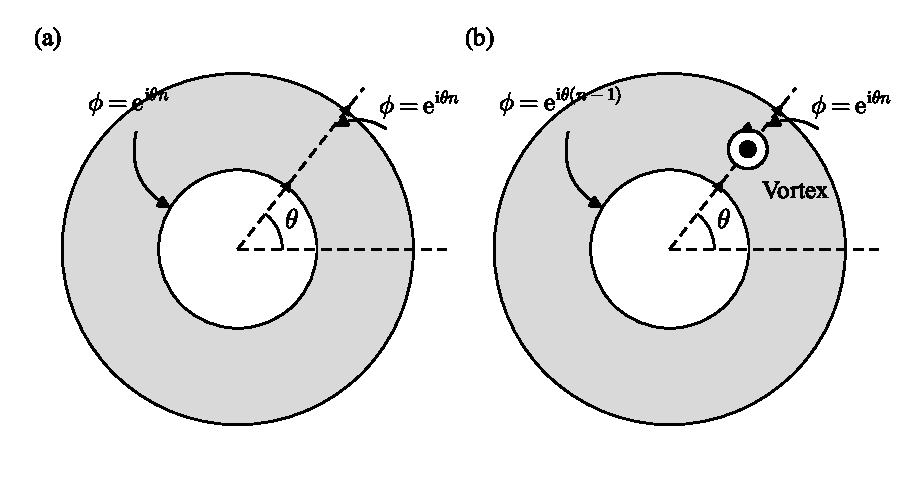
\includegraphics[width=0.72\textwidth]{fig_3.15.pdf}
\caption*{图 3.15\quad (a) 凝聚体的相位绕圆环扭转 $n$ 次，代表一个超流流动。(b) 一个涡旋可以把相位扭转从 $n$ 次变为 $n-1$ 次。}
\end{figure}

有趣的是，自由玻色子的 $v_{c}=0$，即使在零温下也是如此。因此，尽管零温下的自由玻色子具有长程序，但由于 $v_{c}=0$，它们并不形成超流体。

让我们更仔细地考察二流体图像（two-fluid picture）。注意 $m\pmb{v}$ 决定凝聚体的扭转。因此，超流分量中的每个玻色子都携带动量 $m\pmb{v}$，而 $\pmb{P}_{\pmb{v}}/m\pmb{v}$ 给出超流分量中玻色子的数目。我们求得超流密度（superfluid density）为
\begin{equation*}
\rho_{s} = \frac{\pmb{P}_{\pmb{v}}}{\mathcal{V}m\pmb{v}} = \rho - \rho_{n}
\end{equation*}
而 $\rho_{n}$ 可以看作正常流体（normal fluid）的密度。由式 (3.7.13) 我们看到，零温下 $\rho_{s}=\rho$，尽管 $k=0$ 态中玻色子的数目小于 $N$。

如果玻色子带电并与电磁规范场 $A_{\mu}$ 耦合，那么具有零规范势的扭转凝聚体（$\pmb{A}=0$，$\mathrm{e}^{\mathrm{i}m\pmb{v}\cdot\pmb{x}}\varphi_{0}$）与具有非零规范势的无扭转凝聚体（$\pmb{A}=m\pmb{v}$，$\varphi_{0}$）是规范等价的。在这种情形下，式 (3.7.12) 可以解释为：通过打开一个常规范势 $\pmb{A}=m\pmb{v}$ 来产生有限动量 $\pmb{P}_{\pmb{v}}$。由于伽利略不变性（Galileo invariance），动量密度 $\pmb{P}_{\pmb{v}}/\mathcal{V}$ 正比于流密度 $\pmb{j}=\pmb{P}_{\pmb{v}}/m\mathcal{V}$。于是式 (3.7.12) 可以改写为
\begin{equation*}
\pmb{j} = \frac{\rho_{s}}{m}\pmb{A}
\end{equation*}
这正是伦敦方程（London equation）。我们看到，有限温度下伦敦方程中的系数由 $\rho_{s}/m$ 给出，而式 (3.7.13) 使我们能够计算它对温度的依赖关系。

% ---- 书页 135 (p150) ----
\subsection*{问题 3.7.2}
非伽利略不变超流体。尽管上面的讨论集中于伽利略不变的超流体，但所得到的大多数结果同样适用于非伽利略不变的超流体。

\begin{enumerate}
\item 对具有常规范势 $\pmb{A}$ 的玻色子系统导出 XY 模型，假设凝聚体 $\varphi=$ 常数。求出低能模式的色散 $\epsilon_{\pmb{A}}(\pmb{k})$，并与上面得到的 $\epsilon_{\pmb{v}}(\pmb{k})$ 比较。
\item 重复上述计算，但现在在玻色子拉格朗日量中附加一项 $\frac{c}{2}|\dot{\varphi}|^{2}$，以破坏伽利略不变性。
\item 导出上述非伽利略不变系统的伦敦方程。（提示：你可以先导出零温下的伦敦方程，然后考虑有限 $T$ 下的激发如何修正流。注意动量为 $\pmb{k}$ 的激发对流的贡献由 $\frac{\partial}{\partial\pmb{A}}\epsilon_{\pmb{A}}(\pmb{k})$ 给出。）
\end{enumerate}

\subsection{隧穿与约瑟夫森效应}

我们已经看到，超流相中玻色子的格林函数在不同的维度下颇为不同。本节我们将讨论两个超流体或超导体之间的隧穿（tunneling）。我们将看到，隧穿实验使我们能够测量玻色子格林函数的性质。

考虑由 $H_{R}$ 与 $H_{L}$ 描写、并通过一个隧穿算符 $I$ 耦合起来的两个玻色子系统，使得
\begin{equation*}
H = H_{R} + H_{L} + \Gamma I + \Gamma I^{\dagger}
\end{equation*}
其中
\begin{equation*}
I = \varphi_{L}\varphi_{R}^{\dagger}
\end{equation*}
$\Gamma$ 描写隧穿振幅。在存在电磁规范场时，总哈密顿量需要改写为
\begin{equation*}
H = H_{R} + H_{L} + \Gamma\mathrm{e}^{-\mathrm{i}a}I + \Gamma\mathrm{e}^{+\mathrm{i}a}I^{\dagger}
\end{equation*}
其中 $a=\int_{L}^{R}\pmb{A}\,\mathrm{d}\pmb{x}$ 是矢量势沿隧穿结的积分。隧穿流算符由下式给出
\begin{equation*}
j_{T} = \frac{\partial}{\partial a}H = -\mathrm{i}\Gamma\left(I\mathrm{e}^{-\mathrm{i}a} - I^{\dagger}\mathrm{e}^{+\mathrm{i}a}\right)
\end{equation*}
若 $\langle j_{T}\rangle>0$，则电流从 L 流向 R。在 $A_{0}=0$ 规范中，两个系统之间的电压差 $V=V_{L}-V_{R}$ 可以通过令
\begin{equation*}
a(t) = \int_{L}^{R}\pmb{A}\,\mathrm{d}\pmb{x} = -Vt
\end{equation*}
而包括进来。$A_{0}=0$ 规范的优点是，接通电压并不影响 $H_{R,L}$。

% ---- 书页 136 (p151) ----
有了上述设置，我们就可以利用线性响应理论（见式 (2.2.3)）写出隧穿流的如下表达式：
\begin{align*}
\langle j_{T}\rangle(t) ={}& -\mathrm{i}\Gamma\int^{t}\mathrm{d}t'\ \Big\langle\big[j_{T}(t), \big(\mathrm{e}^{-\mathrm{i}a(t')}I(t') + \text{h.c.}\big)\big]\Big\rangle + \langle j_{T}\rangle_{0}(t)\\
={}& -\Gamma^{2}\int^{t}\mathrm{d}t'\ \mathrm{e}^{-\mathrm{i}a(t)}\Big(\mathrm{e}^{\mathrm{i}a(t')}\big\langle[I(t), I^{\dagger}(t')]\big\rangle + \mathrm{e}^{-\mathrm{i}a(t')}\big\langle[I(t), I(t')]\big\rangle + \text{h.c.}\Big)\\
& + \langle j_{T}\rangle_{0}(t)
\end{align*}
其中 $\langle j_{T}\rangle_{0}(t)$ 是在没有隧穿项时的平均。

如果两个玻色子系统都处于超流相或超导相，那么主要贡献来自 $\langle j_{T}\rangle_{0}(t)$：
\begin{equation*}
\langle j_{T}\rangle(t) = 2\Gamma|\varphi_{R}\varphi_{L}|\sin(\theta - a(t))
\end{equation*}
其中 $\theta$ 是两个凝聚体 $\varphi_{R}$ 与 $\varphi_{L}$ 之间的相位差。我们看到，即使在零电压 $a(t)=0$ 时，只要 $\theta\neq0$，隧穿流就可以不为零：
\begin{equation*}
\langle j_{T}\rangle = I_{c}\sin(\theta), \qquad I_{c} = 2\Gamma|\varphi_{R}\varphi_{L}|
\end{equation*}
其中 $I_{c}$ 是最大隧穿流（称为临界隧穿流）。

如果其中一个玻色子系统处于正常相（包括代数衰减相），则 $\langle j_{T}\rangle_{0}(t)=0$ 且 $\langle[I(t), I(t')]\rangle=0$。我们有
\begin{equation*}
\langle j_{T}\rangle(t) = -\Gamma^{2}\int^{t}\mathrm{d}t'\left(\mathrm{e}^{-\mathrm{i}a(t)+\mathrm{i}a(t')}\big\langle[I(t), I^{\dagger}(t')]\big\rangle + \text{h.c.}\right) \tag{3.7.15}
\end{equation*}
由于 $\big\langle[I(t), I^{\dagger}(t')]\big\rangle$ 是没有隧穿时的关联，它可以表示成结两侧格林函数的乘积。例如，
\begin{equation*}
\big\langle I(t)I^{\dagger}(t')\big\rangle = \big\langle\varphi_{L}(t)\varphi_{L}^{\dagger}(t')\big\rangle\big\langle\varphi_{R}^{\dagger}(t)\varphi_{R}(t')\big\rangle
\end{equation*}

在 $1+1$ 维中，编时格林函数具有如下的代数衰减：
\begin{equation*}
\big\langle\varphi_{L,R}(t)\varphi_{L,R}^{\dagger}(t')\big\rangle \sim \mathrm{e}^{-\mathrm{i}\eta_{L,R}\pi/2}\,|t-t'|^{-\eta_{L,R}}.
\end{equation*}

% ---- 书页 137 (p152) ----
我们发现隧穿流具有如下形式\footnote{我们用到了如下事实
\begin{gather*}
\big\langle\varphi_{L,R}(t)\varphi_{L,R}^{\dagger}(t')\big\rangle = \big\langle\varphi_{L,R}^{\dagger}(t)\varphi_{L,R}(t')\big\rangle,\\
\big\langle\varphi_{L,R}^{\dagger}(t')\varphi_{L,R}(t)\big\rangle = \big\langle\varphi_{L,R}^{\dagger}(t)\varphi_{L,R}(t')\big\rangle^{*}
\end{gather*}
来证明
\begin{align*}
\big\langle[I(t), I^{\dagger}(t')]\big\rangle ={}& \big\langle\varphi_{R}^{\dagger}(t)\varphi_{R}(t')\big\rangle\big\langle\varphi_{L}(t)\varphi_{L}^{\dagger}(t')\big\rangle - \big\langle\varphi_{R}(t')\varphi_{R}^{\dagger}(t)\big\rangle\big\langle\varphi_{L}^{\dagger}(t')\varphi_{L}(t)\big\rangle\\
={}& \mathrm{e}^{-\mathrm{i}(\eta_{R}+\eta_{L})\pi/2}\left(\frac{l}{v|t-t'|}\right)^{\eta_{R}+\eta_{L}} - \text{h.c.}\\
={}& -2\mathrm{i}\sin\left(\frac{(\eta_{R}+\eta_{L})\pi}{2}\right)\left(\frac{l}{v|t-t'|}\right)^{\eta_{R}+\eta_{L}}
\end{align*}}
\begin{align*}
\langle j_{T}\rangle ={}& 2\sin\left(\frac{(\eta_{R}+\eta_{L})\pi}{2}\right)\left(\frac{l}{v}\right)^{\eta_{R}+\eta_{L}}\\
&\times \Gamma^{2}\int^{t}\mathrm{d}t'\ \left(\mathrm{i}\,\mathrm{e}^{\mathrm{i}V(t-t')}(t-t')^{-\eta_{R}-\eta_{L}}\frac{1}{|t-t'|^{\eta_{R}+\eta_{L}}} + \text{h.c.}\right)
\end{align*}
它导致一条非线性的 $I$--$V$ 曲线\footnote{我们用到了如下事实
\begin{align*}
\int_{-\infty}^{0}\mathrm{d}t\ \mathrm{e}^{\mathrm{i}Vt}|t|^{-a} ={}& \Big|_{t\to-\mathrm{i}\tau\,\mathrm{sgn}(V)}\ -\mathrm{i}\,\mathrm{sgn}(V)\,\mathrm{e}^{\mathrm{i}a\pi\,\mathrm{sgn}(V)/2}\int_{0}^{+\infty}\mathrm{d}\tau\ \mathrm{e}^{-|V|\tau}\tau^{-a}\\
={}& -\mathrm{i}\,\mathrm{sgn}(V)\,\mathrm{e}^{\mathrm{i}a\pi\,\mathrm{sgn}(V)/2}\,|V|^{a-1}\Gamma(1-a)
\end{align*}
以及 $\Gamma(a)\Gamma(1-a) = \frac{\pi}{\sin(\pi a)}$。}
\begin{equation*}
\langle j_{T}\rangle = 2\left(\frac{l}{v}\right)^{\eta_{R}+\eta_{L}}\Gamma^{2}\frac{\pi}{\Gamma(\eta_{R}+\eta_{L})}\,|V|^{\eta_{R}+\eta_{L}-1}\,\mathrm{sgn}(V)
\end{equation*}
我们看到，代数衰减的指数 $\eta_{R}+\eta_{L}$ 可以在隧穿实验中测量。

\subsection*{问题 3.7.3}
求有限温度下隧穿 $I$--$V$ 曲线的表达式，并证明 $V=0$ 处的微分电导具有温度依赖关系 $\mathrm{d}I/\mathrm{d}V\propto T^{\eta_{R}+\eta_{L}-2}$。

\subsection{Anderson--Higgs 机制}
\begin{keypoints}
\item Anderson--Higgs 机制把无能隙的 Nambu--Goldstone 模与无能隙的规范模结合成一个具有有限能隙的模。
\end{keypoints}

在上面的讨论中，我们把电磁规范场 $A_{\mu}$ 当作一个背景场（background field），它是固定的，不随电荷

% ---- 书页 138 (p153) ----
与流的变化而响应。本节中，我们将把 $A_{\mu}$ 当作一个具有自身涨落的动力学场来处理。

玻色子与规范场的量子理论可以通过路径积分来定义
\begin{equation*}
Z = \int\mathcal{D}\varphi\,\mathcal{D}A_{\mu}\ \mathrm{e}^{\mathrm{i}\int \mathrm{d}^{d}\pmb{x}\,\mathrm{d}t\, L(\varphi,A_{\mu}) + \frac{1}{8\pi e^{2}}(\pmb{E}^{2}-\pmb{B}^{2})}
\end{equation*}
其中我们已令光速 $c=1$。这里 $L(\varphi,A_{\mu})$ 是式 (3.7.3) 给出的加了规范场的玻色子拉格朗日量。本节我们只考虑由
\begin{equation*}
L = L(\varphi,A_{\mu}) + \frac{1}{8\pi e^{2}}(\pmb{E}^{2}-\pmb{B}^{2}) \tag{3.7.16}
\end{equation*}
描写的经典理论。量子规范理论将在第 6 章讨论。

由于规范不变性 (3.7.4)，如果 $(\varphi(\pmb{x},t), A_{\mu}(\pmb{x},t))$ 是运动方程的一个解，那么规范变换后的场 $(\tilde{\varphi}(\pmb{x},t), \tilde{A}_{\mu}(\pmb{x},t))$ 也满足运动方程。在规范理论中，我们不把 $(\varphi(\pmb{x},t), A_{\mu}(\pmb{x},t))$ 与 $(\tilde{\varphi}(\pmb{x},t), \tilde{A}_{\mu}(\pmb{x},t))$ 视为两个不同的运动，而是把它们视为同一个运动。换言之，场 $(\varphi(\pmb{x},t), A_{\mu}(\pmb{x},t))$ 是物理运动的多对一的标记。两组规范等价的场 $(\varphi(\pmb{x},t), A_{\mu}(\pmb{x},t))$ 与 $(\tilde{\varphi}(\pmb{x},t), \tilde{A}_{\mu}(\pmb{x},t))$ 是描写同一运动的两个标记。

在对称性破缺相中，我们有 $|\varphi(\pmb{x},t)|\neq0$。我们可以通过一个规范变换使 $\varphi(\pmb{x},t)$ 成为实数，即 $\varphi(\pmb{x},t)=|\varphi(\pmb{x},t)|=\phi(\pmb{x},t)$。这一手续称为固定规范（fixing the gauge）或选取规范（choosing the gauge）。固定规范之后，不同的 $(\phi, A_{\mu})$ 对将描写物理上不同的运动。在 $\varphi(\pmb{x},t)$ 取实值的规范中，我们有
\begin{equation*}
L = -A_{0}\phi^{2} - \frac{1}{2m}(\partial_{i}\phi)^{2} - \frac{\phi^{2}}{2m}(A_{i})^{2} - V(\phi) + \frac{1}{8\pi e^{2}}(\pmb{E}^{2}-\pmb{B}^{2})
\end{equation*}
把 $\phi=\varphi_{0}+\delta\phi$ 的小涨落积掉之后，我们得到下列低能有效理论：
\begin{equation*}
L_{\mathrm{eff}} = \frac{1}{2V_{0}}(A_{0})^{2} - \frac{\rho}{2m}(A_{i})^{2} + \frac{1}{8\pi e^{2}}(\pmb{E}^{2}-\pmb{B}^{2}) \tag{3.7.17}
\end{equation*}
上式也可以从加了规范场的 XY 模型 (3.7.10) 出发、令 $\theta=0$ 而得到。注意到
\begin{equation*}
\frac{1}{8\pi e^{2}}\pmb{E}^{2} = \frac{1}{8\pi e^{2}}(\partial_{0}A_{i})^{2} + \frac{1}{8\pi e^{2}}(\partial_{i}A_{0})^{2} - \frac{1}{4\pi e^{2}}\partial_{i}A_{0}\partial_{0}A_{i}
\end{equation*}
而 $A_{0}$ 不含时间导数项。因此 $A_{0}$ 不是动力学变量，我们把它积掉，得到
\begin{equation*}
L_{\mathrm{eff}} = \partial_{0}A_{j}\left(\frac{1}{8\pi e^{2}}\delta_{ij} + \frac{1}{2}\,\frac{V_{0}}{(4\pi)^{2}e^{4}}\,\partial_{j}\partial_{i}\right)\partial_{0}A_{i} - \frac{\rho}{2m}A_{i}^{2} - \frac{1}{8\pi e^{2}}\pmb{B}^{2}
\end{equation*}

% ---- 书页 139 (p154) ----
引入横分量与纵分量如下：
\begin{equation*}
A_{i} = \hat{k}_{i}A^{\parallel} + \hat{n}_{a}A_{a}^{\perp} \tag{3.7.18}
\end{equation*}
其中 $\hat{k}$、$\hat{n}_{1}$ 与 $\hat{n}_{2}$ 构成一组局域正交基，我们便可把 $L_{\mathrm{eff}}$ 改写为
\begin{align*}
L_{\mathrm{eff}} ={}& \frac{1}{8\pi e^{2}}\left((\partial_{0}A_{a}^{\perp})^{2} - (\partial_{i}A_{a}^{\perp})^{2}\right) - \frac{\rho}{2m}(A_{a}^{\perp})^{2}\\
&+ \frac{1}{8\pi e^{2}}\,\partial_{0}A^{\parallel}\left(1 + \frac{V_{0}}{4\pi e^{2}}(\partial_{i})^{2}\right)\partial_{0}A^{\parallel} - \frac{\rho}{2m}(A^{\parallel})^{2}.
\end{align*}
由运动方程我们发现，$L_{\mathrm{eff}}$ 所描写的三个模式都具有相同的能隙 $\Delta = e\sqrt{4\pi\rho/m}$。不存在无能隙模式。无能隙规范模式与无能隙 Nambu--Goldstone 模式之间的耦合赋予这些模式有限的能隙。这一现象称为 Anderson--Higgs 机制（Anderson, 1963; Higgs, 1964）。我们还可以把 $\partial_{i}^{2}\partial_{0}^{2}$ 项中的 $\partial_{0}$ 换成 $-\mathrm{i}\Delta$，从而进一步简化 $L_{\mathrm{eff}}$：
\begin{align*}
L_{\mathrm{eff}} ={}& \frac{1}{8\pi e^{2}}\left((\partial_{0}A_{a}^{\perp})^{2} - (\partial_{i}A_{a}^{\perp})^{2}\right) - \frac{\rho}{2m}(A_{a}^{\perp})^{2}\\
&+ \frac{1}{8\pi e^{2}}\left((\partial_{0}A^{\parallel})^{2} - v^{2}(\partial_{i}A^{\parallel})^{2}\right) - \frac{\rho}{2m}(A^{\parallel})^{2} \tag{3.7.19}
\end{align*}
（注意 $v^{2}=V_{0}\rho/m$ 是 XY 模型的速度。）从 $L_{\mathrm{eff}}$ 出发，我们可以研究带电超流体的所有经典电磁性质。

\subsection*{问题 3.7.4}
由拉格朗日量 $L=\frac{1}{8\pi e^{2}}(c^{-1}\pmb{E}^{2}-c\pmb{B}^{2})$ 导出 Maxwell 方程。证明规范涨落是无能隙的，且 $c$ 就是光速。

\section{热势的微扰计算}

\subsection{微扰与费曼规则}
\begin{keypoints}
\item 相互作用玻色子系统的费曼图与费曼规则。
\end{keypoints}

本节我们将讨论如何系统地计算相互作用玻色子系统的热势。为简单起见，我们假设玻色子场是实的。一个复玻色子场可以视为由两个分量组成，其中每个分量都是一个实玻色子场。下面的讨论可以容易地推广到多分量玻色子场。我们从有限温度下的虚时路径积分出发。计算热势的第一步是找到一个经典解 $\varphi_{c}$，并把作用量 $S$ 绕它

% ---- 书页 140 (p155) ----
展开如下：
\begin{equation*}
S(\varphi) = S(\varphi_{c}) + \int_{0}^{\beta}\mathrm{d}x^{\mu}\mathrm{d}y^{\mu}\ \frac{1}{2}\delta\varphi(x^{\mu})\mathcal{K}^{\beta}(x^{\mu}-y^{\mu})\delta\varphi(y^{\mu}) + \int_{0}^{\beta}\mathrm{d}x^{\mu}\,V(\delta\varphi)
\end{equation*}
其中 $V(\delta\varphi)=g_{3}\delta\varphi^{3}+g_{4}\delta\varphi^{4}+\dots$。如果我们忽略高阶项 $V(\delta\varphi)$，我们就得到一个自由系统，其热势 $\Omega_{0}$ 可以通过高斯积分算出，如 3.7.5 节所讨论。为计算相互作用系统的热势，我们注意到
\begin{align*}
Z = A\int\mathcal{D}\varphi\ \mathrm{e}^{-S} ={}& \mathrm{e}^{-S(\varphi_{c})}\mathrm{e}^{-\beta\Omega_{0}}\frac{\int\mathcal{D}\delta\varphi\ \mathrm{e}^{-S_{0}-\int \mathrm{d}x^{\mu}V(\delta\varphi)}}{\int\mathcal{D}\delta\varphi\ \mathrm{e}^{-S_{0}}}\\
={}& \mathrm{e}^{-S(\varphi_{c})}\mathrm{e}^{-\beta\Omega_{0}}\sum_{n=0}\frac{(-)^{n}}{n!}\left\langle\left(\int \mathrm{d}x^{\mu}\,V(\delta\varphi)\right)^{n}\right\rangle_{0}
\end{align*}
其中 $\langle\dots\rangle_{0}$ 表示权重为 $\mathrm{e}^{-S_{0}}$ 的平均，而 $S_{0}$ 是作用量的二次部分，即 $S_{0}\allowbreak=\int_{0}^{\beta}\mathrm{d}x^{\mu}\mathrm{d}y^{\mu}\allowbreak\ \frac{1}{2}\delta\varphi(x^{\mu})\mathcal{K}^{\beta}(x^{\mu}-y^{\mu})\delta\varphi(y^{\mu})$。如果存在若干个经典解（或驻定路径）$\varphi_{c}^{(a)}$，那么我们应当把它们全部包括进来：
\begin{equation*}
Z = \sum_{a}\mathrm{e}^{-S(\varphi_{c}^{(a)})}\mathrm{e}^{-\beta\Omega_{0}^{(a)}}\frac{\int\mathcal{D}\delta\varphi\ \mathrm{e}^{-S_{0}^{(a)}-\int \mathrm{d}x^{\mu}V^{(a)}(\delta\varphi)}}{\int\mathcal{D}\delta\varphi\ \mathrm{e}^{-S_{0}^{(a)}}}
\end{equation*}

我们看到，为计算总热势，我们需要计算多点关联 $\langle\prod_{i=1}^{n}\delta\varphi(i)\rangle_{0}$。对 $n=2$，它就是玻色子场的格林函数 $\langle\delta\varphi(1)\delta\varphi(2)\rangle_{0}=\mathcal{G}^{\beta}(1,2)$，其中 1 与 2 分别代表第一个与第二个玻色子场的坐标 $x_{1}^{\mu}$ 与 $x_{2}^{\mu}$。作为一个算符，$\mathcal{G}^{\beta}(1,2)$ 是 $\mathcal{K}^{\beta}(1,2)$ 的逆，即 $\int \mathcal{G}^{\beta}(1,2)\mathcal{K}^{\beta}(2,3)=\delta(x_{1}^{\mu}-x_{3}^{\mu})$。这里我们还使用了缩写 $\int f(1)\equiv\int \mathrm{d}^{d}x_{1}^{\mu}f(x_{1}^{\mu})$、$\int f(1)g(1,2)\equiv\int \mathrm{d}^{d}x_{1}^{\mu}\mathrm{d}^{d}x_{2}^{\mu}f(x_{1}^{\mu})g(x_{1}^{\mu},x_{2}^{\mu})$ 等。引入生成泛函
\begin{equation*}
Z[j] = \frac{\int\mathcal{D}\delta\varphi\ \mathrm{e}^{-S_{0}-\int \mathrm{d}x^{\mu}j\delta\varphi}}{\int\mathcal{D}\delta\varphi\ \mathrm{e}^{-S_{0}}} = \mathrm{e}^{\frac{1}{2}\int j(1)\mathcal{G}^{\beta}(1,2)j(2)}
\end{equation*}
我们发现（对偶数的 $n$）
\begin{align*}
\left\langle\prod_{i=1}^{n}\delta\varphi(i)\right\rangle_{0} ={}& \frac{\delta^{n}}{\delta j(1)\dots\delta j(n)}Z[j]\Big|_{j=0}\\
={}& \frac{1}{2^{n/2}(n/2)!}\ \frac{\delta^{n}}{\delta j(1)\dots\delta j(n)}\left(\int j\mathcal{G}^{\beta}j\right)^{n/2}\\
={}& \left(\mathcal{G}^{\beta}(1,2)\mathcal{G}^{\beta}(3,4)\dots\mathcal{G}^{\beta}(n-1,n)\right) + \text{所有不同的排列}
\end{align*}
上式是 Wick 定理的另一种形式。

% ---- 书页 141 (p156) ----
\begin{figure}[H]
\centering
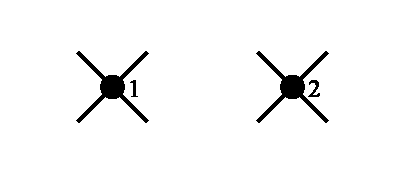
\includegraphics[width=0.72\textwidth]{fig_3.16.pdf}
\caption*{图 3.16\quad 两个顶点，代表 $\int g_{4}\delta\varphi^{4}(1)\int g_{4}\delta\varphi^{4}(2)$。}
\end{figure}

利用 Wick 定理我们发现，例如 $\big\langle\int V(\delta\varphi)\int V(\delta\varphi)\big\rangle_{0}$ 包含许多项：
\begin{align*}
\left\langle\int V(\delta\varphi)\int V(\delta\varphi)\right\rangle_{0} ={}& \left\langle\int g_{4}\delta\varphi^{4}(1)\int g_{4}\delta\varphi^{4}(2)\right\rangle_{0} + \dots\\
={}& \left[4!g_{4}^{2}\int\left(\mathcal{G}^{\beta}(1,2)\right)^{4}\right] + \left[(6^{2}\times 2)g_{4}^{2}\int\left(\mathcal{G}^{\beta}(1,2)\right)^{2}\mathcal{G}^{\beta}(1,1)\mathcal{G}^{\beta}(2,2)\right]\\
&+ \left[3g_{4}\int\left(\mathcal{G}^{\beta}(1,1)\right)^{2}\right]\left[3g_{4}\int\left(\mathcal{G}^{\beta}(2,2)\right)^{2}\right] + \dots \tag{3.8.1}
\end{align*}
积分因子 $4!$、$6^{2}\times2$ 等来自 Wick 展开中恰好具有相同形状的不同项。例如，在一个更简单的情形中，Wick 展开 $\langle ABCD\rangle=\langle AB\rangle\langle CD\rangle+\langle AC\rangle\langle BD\rangle+\langle AD\rangle\langle BC\rangle$ 导致
\begin{align*}
\langle AABB\rangle ={}& \langle AA\rangle\langle BB\rangle + \langle AB\rangle\langle AB\rangle + \langle AB\rangle\langle AB\rangle\\
={}& \langle AA\rangle\langle BB\rangle + 2\langle AB\rangle\langle AB\rangle
\end{align*}
更方便的做法是利用费曼图，通过费曼规则直接得到 Wick 展开 (3.8.1) 的结果。我们不在一般的框架中描述费曼图与费曼规则，而是选择用式 (3.8.1) 给出的具体例子来解释它们。我觉得在实战中理解费曼图与费曼规则更容易。我们在这里要描述的费曼规则是实空间（real-space）费曼规则。动量空间费曼规则将在 5.4.2 节中描述。

为计算 $\big\langle\int g_{4}\delta\varphi^{4}(1)\int g_{4}\delta\varphi^{4}(2)\big\rangle_{0}$，我们从图 3.16 中代表 $\int g_{4}\delta\varphi^{4}(1)\int g_{4}\delta\varphi^{4}(2)$ 的两个顶点出发。为得到期望值 $\langle\dots\rangle_{0}$，我们需要把顶点的所有“腿”彼此连接起来。这就生成了图 3.17 中的图形。这些图形称为费曼图。为构造式 (3.8.1) 的结果，我们只需使用以下三条费曼规则。

(i) 费曼图中的每条线代表一个传播子 $\mathcal{G}^{\beta}(a,b)$，其中 $a$ 与 $b$ 是该线两端的两个顶点。

(ii) 每个顶点代表 $g_{4}\int$。

(iii) 连通图的值由规则 (i) 与 (ii) 给出，而非连通图

% ---- 书页 142 (p157) ----
\begin{figure}[H]
\centering
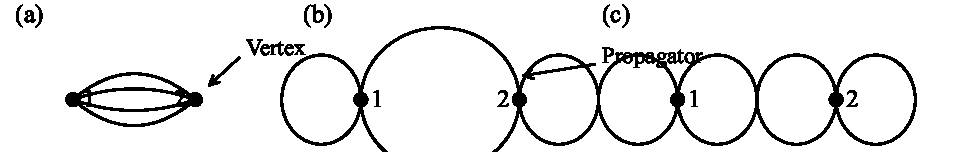
\includegraphics[width=0.72\textwidth]{fig_3.17.pdf}
\caption*{图 3.17\quad 对应于式 (3.8.1) 中三项的三个费曼图。这里 (a) 与 (b) 是连通图，(c) 是包含两个连通图的非连通图。}
\end{figure}

的值由连通子图的乘积给出。这样，我们从图 3.17(a)、(b) 与 (c) 所示的三个费曼图分别得到式 (3.8.1) 末行中的第一、第二与第三项。

嗯，并不完全如此。我们忽略了诸如 $4!$、$6^{2}\times2$ 等数值因子。这些数值因子是费曼规则中最困难的部分。它们从何而来？我们先考虑与图 3.17(a) 中图形相联系的因子 $4!$。这个因子来自这样一个事实：每个顶点有四条腿，而把顶点 1 的四条腿与顶点 2 的四条腿连接起来共有 $4!$ 种不同的方式。与图 3.17(b) 中图形相联系的因子 $6^{2}\times2$ 更复杂一些，但它仍然代表八条腿彼此连接的不同方式。首先，顶点 1 的两条腿彼此相连。从四条腿中选取两条有六种方式，这样我们就得到 $6^{2}\times2$ 中的因子 6。第二个因子 6 类似地来自顶点 2。把顶点 1 剩下的两条腿与顶点 2 剩下的两条腿连接起来有两种方式，于是我们得到最后的因子 2。第三项中的因子 3 对应于把一个顶点的四条腿分成两组、每组各有两条腿的不同分法。（注意这不同于从四条腿中选取两条腿的不同选法。）

让我们回到想要计算的热势。在得到所有的平均之后，相互作用对热势的修正可以这样求出：
\begin{equation*}
\delta\Omega = -T\ln\sum_{n=0}\frac{(-)^{n}}{n!}\left\langle\left(\int \mathrm{d}x^{\mu}\,V(\delta\varphi)\right)^{n}\right\rangle_{0}
\end{equation*}
有一个连链定理（linked-cluster theorem）可以简化上述计算。根据该定理，$\delta\Omega$ 由所有连通图之和给出：
\begin{equation*}
\delta\Omega = -T\sum_{n=0}\frac{(-)^{n}}{n!}\left\langle\left(\int \mathrm{d}x^{\mu}\,V(\delta\varphi)\right)^{n}\right\rangle_{0c}
\end{equation*}
其中 $\big\langle\big(\int \mathrm{d}x^{\mu}V(\delta\varphi)\big)^{n}\big\rangle_{0c}$ 是从 $\big\langle\big(\int \mathrm{d}x^{\mu}V(\delta\varphi)\big)^{n}\big\rangle_{0}$ 中去掉所有非连通图的贡献后得到的。

% ---- 书页 143 (p158) ----
\subsection{连链定理}
\begin{keypoints}
\item 只对连通的费曼图求和，就可以直接计算有效作用量。
\end{keypoints}

我们将用复制（replica）技巧来导出连链定理，这既是为了简洁，也是为了介绍这一有用的方法。复制方法的基本思想是，对整数 $n$，通过把系统复制 $n$ 份来计算 $Z^{n}$：
\begin{equation*}
\left(\frac{Z}{Z_{0}}\right)^{n} = \frac{\int\mathcal{D}\delta\varphi_{\alpha}\ \mathrm{e}^{-\sum_{\alpha=1}^{n}\left[S_{0}(\delta\varphi_{\alpha}) + \int \mathrm{d}x^{\mu}V(\delta\varphi_{\alpha})\right]}}{\int\mathcal{D}\delta\varphi_{\alpha}\ \mathrm{e}^{-\sum_{\alpha=1}^{n}S_{0}(\delta\varphi_{\alpha})}}
\end{equation*}
现在 $(Z/Z_{0})^{n}$ 可以通过微扰展开来计算。在每一个费曼图中，每条传播子都携带一个指标 $\alpha$，并且进入与离开同一个相互作用顶点的所有传播子都具有相同的指标。当我们把 $\alpha$ 从 1 求和到 $n$ 时，显然每个连通图都正比于 $n$，而每个非连通图正比于 $n^{N_{c}}$，其中 $N_{c}$ 是该非连通图中连通图的数目。因此，
\begin{align*}
\left(\frac{Z}{Z_{0}}\right)^{n} ={}& \mathrm{e}^{n\ln\frac{Z}{Z_{0}}} = 1 + n\ln\frac{Z}{Z_{0}} + \sum_{m=2}^{\infty}\frac{(n\frac{Z}{Z_{0}})^{m}}{m!}\\
={}& 1 + n\sum(\text{所有连通图}) + O(n^{2})
\end{align*}
这样我们就证明了连链定理。

\subsection*{问题 3.8.1}
考虑一个非简谐振子 $L=\frac{1}{2}m\dot{x}^{2}-\frac{1}{2}m\omega_{0}^{2}x^{2}-gx^{3}$。计算该系统精确到 $g^{2}$ 阶的有限温度自由能。（提示：在 $\tau$ 空间中做计算可能更容易。）

注意，在微扰论的框架内，上述非简谐振子是一个行为良好的系统。不稳定性来自反弹（bounce）。证明在小 $g$ 极限下，基态的衰变率具有 $\omega_{0}\mathrm{e}^{-\#m^{3}\omega_{0}^{5}/g^{2}}$ 的量级。这样的项不可能出现在围绕基态 $x=0$ 的微扰计算中。然而，反弹作为另一条驻定路径，确实对自由能有贡献。证明反弹的贡献以正比于 $\mathrm{e}^{-\#m^{3}\omega_{0}^{5}/g^{2}}$ 的非微扰项出现。

% ==================================================================
% 新增术语（ch3_g 新增，供术语表追加）：
%   two-fluid picture 二流体图像
%   superfluid density / normal fluid (density) 超流密度 / 正常流体（密度）
%   London equation 伦敦方程
%   Galileo invariance / Galileo non-invariant 伽利略不变性 / 非伽利略不变的
%   twist 扭转
%   tunneling / tunneling junction / tunneling amplitude 隧穿 / 隧穿结 / 隧穿振幅
%   tunneling current / critical tunneling current 隧穿流 / 临界隧穿流
%   algebraic-decay phase 代数衰减相
%   time-ordered Green's function 编时格林函数
%   I–V curve / differential conductance I–V 曲线 / 微分电导
%   background field / dynamical field 背景场 / 动力学场
%   fixing the gauge / choosing the gauge 固定规范 / 选取规范
%   transverse / longitudinal component 横分量 / 纵分量
%   Feynman diagram / Feynman rules 费曼图 / 费曼规则
%   real-space / momentum-space Feynman rules 实空间 / 动量空间费曼规则
%   vertex / leg（顶点的）腿  顶点
%   connected / disconnected diagram 连通图 / 非连通图
%   linked-cluster theorem 连链定理（术语表已有）
%   replica technique 复制技巧
%   anharmonic oscillator 非简谐振子
%   Maxwell equation Maxwell 方程
%   thermal potential 热势（术语表已有）
% ==================================================================

 % 本文件由 scripts/assemble.py 自动装配，勿手改（改 parts/ 后重跑）
% 第4章 自由费米子系统

% 第4章 FREE FERMION SYSTEMS
\chapter{自由费米子系统}

费米子系统是凝聚态物理中最重要的系统之一。金属、半导体、磁体、超导体等等都是费米子系统，它们的性质主要受电子的费米统计控制。在本章中，我们将研究自由多费米子系统的一些性质。

\section{多费米子系统}

\subsection{什么是费米子？}

\begin{keypoints}
\item 费米子由泡利不相容原理以及一种在两个全同费米子交换时产生$\pi$相移的跃迁哈密顿量来表征。
\item 费米子之所以怪异，是因为它们是非局域的客体。
\item 费米子可以用反对易算符来描述。
\end{keypoints}

长期以来，我们一直觉得自己知道费米子是什么。在读完接下来几节之后，如果你开始觉得自己并不真正理解费米子究竟是什么，那么我就达到了目的。我们将在第10章的后面对"费米子是什么"给出一个回答。这里我们只用传统的方式引进费米子，并在传统图像之内展示费米子是多么奇怪、多么不自然。

我们先尝试描述格点上的无自旋费米子系统。由于泡利不相容原理，格点费米子系统的希尔伯特空间可以用基矢$\{|n_{\pmb{i}_1},n_{\pmb{i}_2},\ldots\rangle\}$展开，其中$n_{\pmb{i}}=0,1$是格点$\pmb{i}$上的费米子数目。为了对自由费米子系统给出二次量子化的描述，我们为每个格点$\pmb{i}$引入湮灭算符$\sigma_{\pmb{i}}^{-}$和产生算符$\sigma_{\pmb{i}}^{+}$。它们具有如下矩阵形式：
\begin{equation*}
\sigma_{\pmb{i}}^{-}=\begin{pmatrix}0 & 0\\ 1 & 0\end{pmatrix}=\frac{1}{2}(\sigma^{x}-\mathrm{i}\sigma^{y})
\qquad
\sigma_{\pmb{i}}^{+}=\begin{pmatrix}0 & 1\\ 0 & 0\end{pmatrix}=\frac{1}{2}(\sigma^{x}+\mathrm{i}\sigma^{y})
\end{equation*}
其中$\sigma^{x,y,z}$是泡利矩阵。湮灭算符$\sigma^{-}$把有一个费米子的态$|1\rangle=\binom{1}{0}$变成没有费米子的态$|0\rangle=\binom{0}{1}$。由于$\sigma_{\pmb{i}}^{\pm}$产生/湮灭一个费米子，我们暂且把它们称作"费米子"算符。

利用"费米子"算符$\sigma_{\pmb{i}}^{\pm}$，我们可以为费米系统写下如下哈密顿量：
\begin{equation*}
H_b=\sum_{\langle\pmb{i}\pmb{j}\rangle}(t_{\pmb{i}\pmb{j}}\sigma_{\pmb{i}}^{+}\sigma_{\pmb{j}}^{-}+\text{h.c.})
\end{equation*}
虽然从数学上看，$H_b$是作用于费米子希尔伯特空间$\{|n_{\pmb{i}_1},n_{\pmb{i}_2},\ldots\rangle\}$之内的厄米算符，但由$H_b$所描述的系统并不是费米子系统，它其实是一个硬核玻色子（hard-core boson）系统或自旋-1/2系统。

这是因为我们的费米子希尔伯特空间同样可以看作一个硬核玻色子的希尔伯特空间，其中$|0\rangle$是零玻色子态，$|1\rangle$是单玻色子态。\footnote{费米子希尔伯特空间也可以看作一个自旋-1/2的希尔伯特空间，其中$|0\rangle$是自旋向下态，$|1\rangle$是自旋向上态。}所以，单凭希尔伯特空间本身，我们无法判断该系统是费米子系统还是玻色子系统；我们必须考察哈密顿量，才能判断系统是费米型的还是玻色型的。哈密顿量$H_b$是用$\sigma_{\pmb{i}}^{\pm}$写出的，而$\sigma_{\pmb{i}}^{\pm}$在不同格点上彼此对易，因此由$H_b$描述的系统是玻色子系统。我们其实应该把$\sigma_{\pmb{i}}^{-}$称作玻色子算符。

令人十分惊讶的是，费米子希尔伯特空间中一个自然的局域哈密顿量所描述的竟然不是费米子系统！这就引出一个有趣的问题：是什么使一个多粒子系统成为费米子系统？显然，仅有泡利不相容原理是不够的。一个费米系统不仅拥有满足泡利不相容原理的费米型希尔伯特空间，它的哈密顿量还具有一种非常特殊的性质。事实上，费米子系统是由高度非局域的哈密顿量
\begin{equation*}
H_f=\sum_{\langle\pmb{i}\pmb{j}\rangle}(\hat{t}_{\pmb{i}\pmb{j}}(\{\sigma_{\pmb{i}'}^{z}\})\sigma_{\pmb{i}}^{+}\sigma_{\pmb{j}}^{-}+\text{h.c.})
\end{equation*}
描述的，其中$\hat{t}_{\pmb{i}\pmb{j}}$是$\sigma_{\pmb{i}}^{z}$算符的函数，它包含许多个$\sigma_{\pmb{i}}^{z}$算符的乘积。对于一个有$N_s$个格点的$d$维格子，$\sigma_{\pmb{i}}^{z}$算符的数目是$N_s^{d-1}$的量级。如果不是大自然为我们提供了这样的非局域系统，任何头脑正常的物理学家都不会想去研究它们。既然这类非局域系统确实存在于自然界，我们就不得不研究它们。可是怎么研究呢？

这里我们极为幸运。自然界中的非局域费米子系统具有一些特殊的性质，使我们能够把它们简化。为了写下简化后的哈密顿量，我们先按某种方式给所有格点排序：$(\pmb{i}_1,\pmb{i}_2,\ldots,\pmb{i}_a,\ldots)$。然后我们引入另一类费米子算符：
\begin{equation*}
c_{\pmb{i}_a}=\sigma_{\pmb{i}_a}^{-}\prod_{b<a}\sigma_{\pmb{i}_b}^{z}\tag{4.1.1}
\end{equation*}
如果我们把格点排序得当，那么用$c_{\pmb{i}}$写出时，$H_f$将取如下较简单的形式：
\begin{equation*}
H_f=\sum_{\langle\pmb{i}\pmb{j}\rangle}(t_{\pmb{i}\pmb{j}}c_{\pmb{i}}^{\dagger}c_{\pmb{j}}+\text{h.c.})\tag{4.1.2}
\end{equation*}
其中$t_{\pmb{i}\pmb{j}}$不依赖于$\sigma_{\pmb{i}}^{z}=2c_{\pmb{i}}^{\dagger}c_{\pmb{i}}-1$。可以验证
\begin{align*}
&\{c_{\pmb{i}},c_{\pmb{j}}\}=\{c_{\pmb{i}}^{\dagger},c_{\pmb{j}}^{\dagger}\}=0\\
&\{c_{\pmb{i}},c_{\pmb{j}}^{\dagger}\}=\delta_{\pmb{i}\pmb{j}}\tag{4.1.3}
\end{align*}
其中$\{A,B\}\equiv AB+BA$称为反对易子（anti-commutator）。玻色子算符$\sigma^{x,y,z}$与费米子算符$c_{\pmb{i}}$之间的这一映射就是Jordan--Wigner变换（Jordan and Wigner, 1928）。我们注意到$c_{\pmb{i}}^{\dagger}c_{\pmb{i}}=\sigma_{\pmb{i}}^{+}\sigma_{\pmb{i}}^{-}$。这里$|0\rangle$和$|1\rangle$是$c_{\pmb{i}}^{\dagger}c_{\pmb{i}}$的两个本征态，本征值分别为0和1。因此，$c_{\pmb{i}}^{\dagger}c_{\pmb{i}}$是格点$\pmb{i}$上的费米子数算符。

通常，我们不去谈论费米子从何而来，而是直接把式(4.1.3)和式(4.1.2)当作自由费米子系统的定义。但如果我们真的追问费米子从何而来，并且认为玻色子比费米子更为基本，\footnote{玻色子系统的定义见10.1节。}那么上面的讨论表明，\emph{费米子是非局域激发}。事实上，自然界中的费米子的确表现得像非局域激发，因为费米子不能被单独产生。大自然似乎想要随时掌握我们宇宙中费米子的总数，以保证这个数是偶整数。局域激发不可能具有这样一种非局域的约束。在第10章中我们将看到，费米子可以解释为凝聚弦的端点，确实是非局域的。

\subsection{自由费米子系统的精确解}

\begin{keypoints}
\item 自由费米子系统的全部本征态和能量本征值都可以由费米子算符的反对易代数得到。
\end{keypoints}

在一个有$N_{\mathrm{site}}$个格点的格子上，费米子系统的希尔伯特空间有$2^{N_{\mathrm{site}}}$个态。哈密顿量(4.1.2)是一个$2^{N_{\mathrm{site}}}\times 2^{N_{\mathrm{site}}}$矩阵。求解该哈密顿量就相当于求出这么大一个矩阵的本征值和本征矢。

利用反对易代数(4.1.3)，可以把哈密顿量(4.1.2)严格解出。为简单起见，让我们假设系统具有平移对称性。此时$t_{\pmb{i}\pmb{j}}$只依赖于差$\pmb{i}-\pmb{j}$，即$t_{\pmb{i},\pmb{i}+\Delta\pmb{i}}=t_{\Delta\pmb{i}}$。引入$c_{\pmb{k}}=\sum_{\pmb{i}}N_s^{-1/2}\mathrm{e}^{-\mathrm{i}\pmb{k}\cdot\pmb{i}}c_{\pmb{i}}$，其中$N_s$是格点总数，我们发现
\begin{align*}
&H_f=\sum_{\pmb{k}}\epsilon_{\pmb{k}}c_{\pmb{k}}^{\dagger}c_{\pmb{k}},\qquad \epsilon_{\pmb{k}}=\sum_{\Delta\pmb{i}}t_{\Delta\pmb{i}}\mathrm{e}^{\mathrm{i}\pmb{k}\cdot\Delta\pmb{i}},\\
&\{c_{\pmb{k}},c_{\pmb{k}'}\}=\{c_{\pmb{k}}^{\dagger},c_{\pmb{k}'}^{\dagger}\}=0,\qquad \{c_{\pmb{k}},c_{\pmb{k}'}^{\dagger}\}=\delta_{\pmb{k}\pmb{k}'}.\tag{4.1.4}
\end{align*}
可以验证，满足$c_{\pmb{k}}|0\rangle=0$的态$|0\rangle$是$H_f$的零本征值本征态。利用反对易关系，我们发现态$|\{n_{\pmb{k}}\}\rangle\equiv\prod_{\pmb{k}}(c_{\pmb{k}}^{\dagger})^{n_{\pmb{k}}}|0\rangle$（$n_{\pmb{k}}=0,1$）是$c_{\pmb{k}}^{\dagger}c_{\pmb{k}}$的共同本征态，即$c_{\pmb{k}}^{\dagger}c_{\pmb{k}}|\{n_{\pmb{k}}\}\rangle=n_{\pmb{k}}|\{n_{\pmb{k}}\}\rangle$，而且它还是能量$E=\sum_{\pmb{k}}n_{\pmb{k}}\epsilon_{\pmb{k}}$的本征态。上面这种形式的本征态给出了$H_f$的全部本征态。这里的$n_{\pmb{k}}$是动量$\pmb{k}$上的费米子占据数。往$\pmb{k}_0$能级上加一个费米子，总能量就增加$\epsilon_{\pmb{k}_0}$，因此$\epsilon_{\pmb{k}_0}$可以解释为单粒子能量。

值得注意的是，我们通过代数途径就得到了$H_f$的全部本征态，而无需显式写出本征矢。对易的玻色代数和反对易的费米代数，是我们能够严格求解的仅有的几个代数系统中的两个。实际上，在相当长的时间里，它们曾是我们能在一维以外严格求解的仅有的两个代数系统。找到一维以外精确可解的代数系统，对我们理解相互作用系统极为重要。第10章将讨论最近发现的另外一些能够在一维以外求解的代数系统（Kitaev, 2003; Levin and Wen, 2003; Wen, 2003c）。这些代数系统引出了一维以外精确可解的相互作用模型。

如果计入化学势$\mu$，自由费米子系统的哈密顿量将变为
\begin{equation*}
H=\sum_{\pmb{k}}(\epsilon_{\pmb{k}}-\mu)c_{\pmb{k}}^{\dagger}c_{\pmb{k}}=\sum_{\pmb{k}}\xi_{\pmb{k}}c_{\pmb{k}}^{\dagger}c_{\pmb{k}},\qquad \xi_{\pmb{k}}\equiv\epsilon_{\pmb{k}}-\mu\tag{4.1.5}
\end{equation*}
$H$的基态由一个态$|\Psi_0\rangle$给出：所有$\xi_{\pmb{k}}<0$的$\pmb{k}$态都被填满，所有$\xi_{\pmb{k}}>0$的$\pmb{k}$态都空着。$|\Psi_0\rangle$由如下代数关系定义：
\begin{equation*}
\begin{aligned}
c_{\pmb{k}}|\Psi_0\rangle&=0,\qquad \text{当 }\xi_{\pmb{k}}>0\\
c_{\pmb{k}}^{\dagger}|\Psi_0\rangle&=0,\qquad \text{当 }\xi_{\pmb{k}}<0
\end{aligned}
\end{equation*}
占据数$n_{\pmb{k}}=c_{\pmb{k}}^{\dagger}c_{\pmb{k}}$在费米面处有一个跃变（见图4.1）。

\begin{figure}[H]
\centering
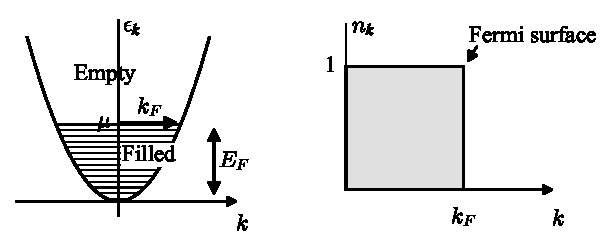
\includegraphics[width=0.72\textwidth]{fig_4.1.pdf}
\caption*{图 4.1\quad 自由费米子系统的基态是一个费米海（Fermi sea）。这里的$E_F$称为费米能，$k_F$称为费米动量。占据数$n_k=n_F(\xi_k)$在费米动量$k_F$处不连续。}
\end{figure}

\subsection*{问题 4.1.1}

\textbf{Jordan--Wigner变换}\quad 由式(4.1.1)证明式(4.1.3)。

\subsection*{问题 4.1.2}

\textbf{一维超导体的能谱}\quad 一维超导体由如下自由费米子哈密顿量描述：
\begin{equation*}
H=\sum_{i}(t\,c_{i}^{\dagger}c_{i+1}+\eta\,c_{i}^{\dagger}c_{i+1}^{\dagger}+\text{h.c.})\tag{4.1.6}
\end{equation*}
证明：在动量空间中，算符
\begin{equation*}
\lambda_{k}=u_{k}c_{k}+v_{k}c_{-k}^{\dagger}
\end{equation*}
满足费米子反对易关系$\{\lambda_{k},\lambda_{k'}\}=\{\lambda_{k}^{\dagger},\lambda_{k'}^{\dagger}\}=0$，并且当$|u_{k}|^{2}+|v_{k}|^{2}=1$时$\{\lambda_{k},\lambda_{k'}^{\dagger}\}=\delta_{kk'}$。证明：通过适当选取$u_{k}$和$v_{k}$，我们可以把$H$改写为
\begin{equation*}
H=E_{g}+\sum_{k}E_{k}\lambda_{k}^{\dagger}\lambda_{k}.
\end{equation*}
求出准粒子激发谱$E_{k}$和基态能量$E_{g}$。

\subsection*{问题 4.1.3}

\textbf{用Jordan--Wigner变换求解一维自旋-1/2系统（或硬核玻色子系统）}\quad 考虑一个具有如下哈密顿量的一维自旋-1/2系统（或硬核玻色子系统）：
\begin{equation*}
H=\sum_{i}\left(J_{x}\sigma_{i}^{x}\sigma_{i+1}^{x}+J_{y}\sigma_{i}^{y}\sigma_{i+1}^{y}+B\sigma_{i}^{z}\right)
\end{equation*}
\begin{enumerate}
\item 用Jordan--Wigner变换（对一维格子取自然排序），把上述相互作用的自旋-1/2（或硬核玻色子）系统映射为一个自由费米子系统。
\item 设$J_x=J_y=J$且$B\neq 0$。当$J$从$-\infty$变到$+\infty$时，系统经历几次相变。求出这些相变的临界$J$值。对每一个相和每一个临界点，画出总能量--动量空间中系统存在激发的区域。所有低能激发都应当包括在内，不论其动量多大；高能激发则不必包括。（提示：应当先思考并猜测一下，根据我们对一维相互作用玻色子系统的知识，谱应当是什么样子。）
\item 设$J_x=\alpha J_y=J$（$0<\alpha<1$）且$B\neq 0$。当$J$从$-\infty$变到$+\infty$时，系统经历几次相变。求出这些相变的临界$J$值。对每一个相和每一个临界点，画出总能量--动量空间中系统存在激发的区域。所有低能激发都应当包括在内，不论其动量多大。
\item 讨论为什么上述两种情形，即$J_x=J_y$与$J_x\neq J_y$，在定性上是不同的。
\end{enumerate}

\subsection{马约拉纳费米子}

自由费米子系统(4.1.2)是一个精确可解的多体系统，其希尔伯特空间的维数为$2^{N_{\mathrm{site}}}$（即每个格点两个态）。还有一个更小的精确可解系统，其希尔伯特空间中只有$2^{N_{\mathrm{site}}/2}$个态（假定$N_{\mathrm{site}}$为偶数）。这个系统称为马约拉纳费米子（Majorana fermion）系统，由如下哈密顿量描述：
\begin{equation*}
H=\sum_{i}(-\mathrm{i}t\,\lambda_{i}\lambda_{i+1}+\text{h.c.})\tag{4.1.7}
\end{equation*}
其中满足
\begin{equation*}
\{\lambda_{i},\lambda_{j}\}=\delta_{ij},\qquad (\lambda_{i})^{\dagger}=\lambda_{i}\tag{4.1.8}
\end{equation*}
的$\lambda_{i}$是马约拉纳费米子算符。马约拉纳费米子系统的希尔伯特空间构成上述反对易代数的一个表示。

为了构造希尔伯特空间，让我们考虑一个有$N_{\mathrm{site}}$个格点的一维周期系统，并假定$N_{\mathrm{site}}$为偶数，而且$\lambda_{i}$满足反周期边界条件$\lambda_{i+N_{\mathrm{site}}}=-\lambda_{i}$。在$k$空间中，哈密顿量(4.1.7)取如下形式：
\begin{equation*}
H=-\sum_{k}\mathrm{i}t\,\mathrm{e}^{\mathrm{i}k}\lambda(-k)\lambda(k)=\sum_{k>0}t\sin k\,\lambda^{\dagger}(k)\lambda(k)
\end{equation*}
其中$\lambda(k)=N_{\mathrm{site}}^{-1/2}\sum_{n}\mathrm{e}^{-\mathrm{i}kn}\lambda_{n}$，而$k=\pm\pi/N_{\mathrm{site}},\pm3\pi/N_{\mathrm{site}},\ldots,\pm(N_{\mathrm{site}}-1)\pi/N_{\mathrm{site}}$。可以验证
\begin{equation*}
\{\lambda^{\dagger}(k),\lambda(k')\}=\delta_{k-k'},\qquad \lambda^{\dagger}(k)=\lambda(-k)
\end{equation*}
我们看到，$k>0$的$\lambda(k)$满足复费米子的反对易代数。令$|0\rangle$为满足$\lambda(k)|0\rangle=0$（对$k>0$）的态。我们可以把$|0\rangle$看作没有费米子的态。令$|\{n_k\}\rangle=\prod_{k>0}(\lambda^{\dagger}(k))^{n_k}|0\rangle$，其中$n_k=0,1$。由于$\lambda^{\dagger}(k)\lambda(k)|\{n_k\}\rangle=n_k|\{n_k\}\rangle$，我们可以把$n_k$看作能级$k$上的占据数。注意，能级只有$N_{\mathrm{site}}/2$个，因为能级由正$k$标记（见图4.2）。因此，希尔伯特空间有$2^{N_{\mathrm{site}}/2}$个态。有趣的是，马约拉纳系统每个格点只有$\sqrt{2}$个态！态$|\{n_k\}\rangle$是一个能量本征态，能量为$\sum_{k>0}2t\sin(k)n_k$。

\begin{figure}[H]
\centering
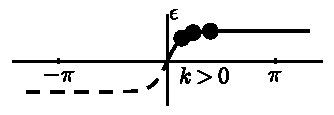
\includegraphics[width=0.72\textwidth]{fig_4.2.pdf}
\caption*{图 4.2\quad 马约拉纳费米子的单粒子能级仅对$k>0$存在。多体态由这些单粒子能级上的占据数$n_k$描述。}
\end{figure}

对于一个具有两个马约拉纳费米子的系统
\begin{equation*}
H=\sum_{i}(-\mathrm{i}t\,\lambda_{1,i}\lambda_{1,i+1}-\mathrm{i}t\,\lambda_{2,i}\lambda_{2,i+1}+\text{h.c.}),
\end{equation*}
其多体希尔伯特空间有$2^{N_{\mathrm{site}}}$个态（即每个格点$\sqrt{2}\times\sqrt{2}=2$个态），与一个复费米子的希尔伯特空间相同。事实上，两个马约拉纳费米子的系统等价于一个复费米子的系统（见问题4.1.4）。

\subsection*{问题 4.1.4}

超导哈密顿量(4.1.6)也可以用马约拉纳费米子算符求解。马约拉纳费米子算符无非就是复费米子算符$c_{i}$的实部和虚部：
\begin{equation*}
\lambda_{1,i}=\frac{c_{i}+c_{i}^{\dagger}}{\sqrt{2}},\qquad \lambda_{2,i}=\frac{c_{i}-c_{i}^{\dagger}}{\mathrm{i}\sqrt{2}}
\end{equation*}
证明$\lambda_{ai}$满足马约拉纳费米子的反对易代数。用马约拉纳费米子求出所有能量本征态及其能量本征值，并把你的结果与问题4.1.2中得到的结果进行比较。

\subsection{跃迁算符的统计代数}

\begin{keypoints}
\item 全同粒子的统计性由其跃迁算符的代数决定。
\end{keypoints}

通常，玻色子系统被定义为由对易算符描述的系统，而费米子系统被定义为由反对易算符描述的系统。然而，这些定义太形式化了。为了从物理上理解玻色子系统与费米子系统的差别，我们考虑下面这个多体跃迁系统。希尔伯特空间由零粒子态$|0\rangle$、单粒子态$|\pmb{i}_1\rangle$、两粒子态$|\pmb{i}_1,\pmb{i}_2\rangle$等等构成，其中$\pmb{i}_n$标记格子中的格点。作为一个全同粒子系统，态$|\pmb{i}_1,\pmb{i}_2,\ldots\rangle$不依赖于指标$\pmb{i}_1,\pmb{i}_2,\ldots$的次序，例如$|\pmb{i}_1,\pmb{i}_2\rangle=|\pmb{i}_2,\pmb{i}_1\rangle$。没有双重占据的格点，并且我们约定当$\pmb{i}_m=\pmb{i}_n$时$|\pmb{i}_1,\pmb{i}_2,\ldots\rangle=0$。

跃迁算符$\hat{t}_{ij}$定义如下：当$\hat{t}_{ij}$作用在态$|\pmb{i}_1,\pmb{i}_2,\ldots\rangle$上时，如果格点$j$上有一个粒子而格点$i$上没有粒子，那么$\hat{t}_{ij}$就把$j$上的粒子搬到$i$，并在所得的态上乘一个复振幅$t(i,j;i_1,i_2,\ldots)$。注意，这个振幅可以依赖于所有粒子的位置，因而不一定是局域的。除此情形之外，跃迁算符$\hat{t}_{ij}$湮灭该态。我们系统的哈密顿量为
\begin{equation*}
H=\sum_{\langle ij\rangle}\hat{t}_{ij}
\end{equation*}
\begin{figure}[H]
\centering
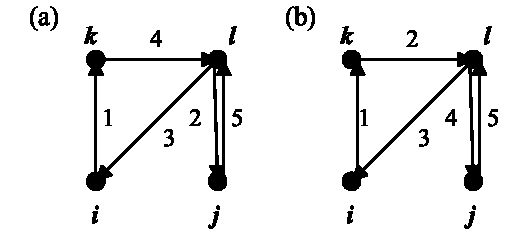
\includegraphics[width=0.72\textwidth]{fig_4.3.pdf}
\caption*{图 4.3\quad (a)五次跃迁的第一种排序方式交换$i$、$j$处的两个粒子。(b)同样五次跃迁的第二种排序方式不交换这两个粒子。}
\end{figure}
其中求和$\sum_{\langle ij\rangle}$遍及某一组配对$\langle ij\rangle$，例如最近邻配对。为了使上述哈密顿量描述一个局域系统，我们要求：当$i$、$j$、$k$、$l$互不相同时，
\begin{equation*}
[\hat{t}_{ij},\hat{t}_{kl}]=0
\end{equation*}
现在的问题是：上述跃迁哈密顿量描述的是硬核玻色子系统还是费米子系统？

多体跃迁系统是玻色子系统还是费米子系统（甚至是其他某种统计系统），与希尔伯特空间毫无关系。多体态由对称化的指标标记（例如$|\pmb{i}_1,\pmb{i}_2\rangle=|\pmb{i}_2,\pmb{i}_1\rangle$）这一事实，并不意味着多体系统就是玻色子系统，正如我们在4.1.1节中已经看到的。统计性由哈密顿量$H$决定。

显然，当跃迁振幅$t(i,j;i_1,i_2,\ldots)$只依赖于$i$和$j$，即$t(i,j;i_1,i_2,\ldots)=t(i,j)$时，多体跃迁哈密顿量描述的是硬核玻色子系统。问题是：在什么条件下多体跃迁哈密顿量描述费米子系统？

Levin和Wen（2003）解决了这个问题。他们发现，只要对任意三个跃迁算符$\hat{t}_{lj}$、$\hat{t}_{il}$、$\hat{t}_{lk}$（其中$i$、$j$、$k$、$l$互不相同），跃迁算符满足
\begin{equation*}
\hat{t}_{lk}\hat{t}_{il}\hat{t}_{lj}=-\hat{t}_{lj}\hat{t}_{il}\hat{t}_{lk}\tag{4.1.9}
\end{equation*}
多体跃迁哈密顿量就描述一个费米子系统。（注意该代数具有$\hat{t}_1\hat{t}_2\hat{t}_3=-\hat{t}_3\hat{t}_2\hat{t}_1$的结构。）

考虑态$|\pmb{i},\pmb{j},\ldots\rangle$，其中$i$、$j$处各有一个粒子，可能还有其他粒子在更远处。我们把一组五个跃迁算符$\{\hat{t}_{jl},\hat{t}_{lk},\hat{t}_{il},\hat{t}_{lj},\hat{t}_{ki}\}$按不同的次序作用到态$|\pmb{i},\pmb{j},\ldots\rangle$上（见图4.3）：
\begin{align*}
\hat{t}_{jl}\hat{t}_{lk}\hat{t}_{il}\hat{t}_{lj}\hat{t}_{ki}|\pmb{i},\pmb{j},\ldots\rangle&=C_1|\pmb{i},\pmb{j},\ldots\rangle\\
\hat{t}_{jl}\hat{t}_{lj}\hat{t}_{il}\hat{t}_{lk}\hat{t}_{ki}|\pmb{i},\pmb{j},\ldots\rangle&=C_2|\pmb{i},\pmb{j},\ldots\rangle
\end{align*}
其中我们假定格点$k$和$l$上没有粒子。我们注意到，五次跃迁之后我们回到原来的态$|\pmb{i},\pmb{j},\ldots\rangle$，只多出了相位$C_{1,2}$。然而从图4.3可以看到，五次跃迁的第一种排序方式（图4.3(a)）交换了$i$、$j$处的两个粒子，而第二种方式（图4.3(b)）不交换这两个粒子。既然两种跃迁方案使用的是同一组五次跃迁，$C_1$与$C_2$之间的差别就来自两个粒子的交换。因此，要使多体跃迁哈密顿量描述费米子系统，必须要求$C_1=-C_2$。注意到两种方案中第一次跃迁和最后一次跃迁是相同的，我们发现：只要跃迁算符满足式(4.1.9)，就有$C_1=-C_2$。事实上，如果我们不想使用反对易代数，式(4.1.9)可以作为费米统计的另一种定义。

我们想指出，在二维格子上，费米子跃迁代数可以推广为更一般的跃迁算符统计代数：
\begin{equation*}
\hat{t}_{ji}\hat{t}_{ik}\hat{t}_{li}=\mathrm{e}^{\mathrm{i}\theta}\hat{t}_{li}\hat{t}_{ik}\hat{t}_{ji}\tag{4.1.10}
\end{equation*}
在这种情形下，多体跃迁哈密顿量描述的是一个统计角为$\theta$的任意子（anyon）系统。

\subsection*{问题 4.1.5}

证明费米子跃迁算符$\hat{t}_{ij}=c_{i}^{\dagger}c_{j}$满足费米子跃迁代数。

\subsection*{问题 4.1.6}

我们已知弦算符（string operator）$\hat{W}_{ij}=\hat{t}_{il}\hat{t}_{lm}\ldots\hat{t}_{nj}$在$i$处产生一个粒子、在$j$处湮灭一个粒子，于是我们可能想把它写成$\hat{W}_{ij}=C_{i}^{+}C_{j}^{-}$。

\begin{enumerate}
\item[(a)] 证明：如果跃迁算符$\hat{t}_{ij}$满足费米子跃迁代数(4.1.9)，则弦算符满足$\hat{W}_{lk}\hat{W}_{il}\allowbreak\hat{W}_{lj}\allowbreak=-\hat{W}_{lj}\allowbreak\hat{W}_{il}\allowbreak\hat{W}_{lk}$。（可以假定这三条弦只在一点$l$相交。）
\item[(b)] 证明$C_{i}^{\pm}$与$C_{j}^{\pm}$不能对易，即使$i$与$j$相距很远。但是，如果$C_{i}^{\pm}$与$C_{j}^{\pm}$反对易（当$i\neq j$时），则费米子跃迁代数(4.1.9)可以得到满足。
\end{enumerate}

\section{自由费米子格林函数}

\begin{keypoints}
\item 格林函数在很长时间上的代数衰减与跨费米面的无能隙激发有关；长距离上的代数衰减与动量空间中的尖锐特征（不连续性）有关。
\item 电子格林函数可以在隧穿实验中测量。
\item 电子格林函数的谱函数。
\end{keypoints}

在接下来的几节中，我们将讨论自由费米子系统的单体和两体关联函数。单体关联函数对理解隧穿和光电子发射（photoemission）实验十分重要。两体关联函数则更为重要，因为它们与各种各样的输运、散射以及线性响应实验都有关系。在这两节中我会给出一些计算细节。这些讨论的目的主要是引进数学形式。我们列出了$d=1,2,3$维的许多显式结果，希望这些结果既可以用作参考，也可以作为各种关联的具体例子。

\subsection{编时关联函数}

\begin{keypoints}
\item 在编时平均之下，费米子算符表现得像反对易的数。
\end{keypoints}

考虑由式(4.1.5)描述的自由费米子系统。在海森堡绘景中，含时的费米子算符为
\begin{equation*}
c_{\pmb{k}}(t)=U^{\dagger}(t,-\infty)c_{\pmb{k}}U(t,-\infty),\qquad U(t_1,t_2)=\mathrm{e}^{-\mathrm{i}\int_{t_2}^{t_1}\mathrm{d}t\, H}
\end{equation*}
零温和有限温下的费米子传播子（即格林函数）定义为编时平均
\begin{align*}
\mathrm{i}G(t_1-t_2,\pmb{k}_1)\delta_{\pmb{k}_1,\pmb{k}_2}&=\langle 0|T(c_{\pmb{k}_1}(t_1)c_{\pmb{k}_2}^{\dagger}(t_2))|0\rangle\tag{4.2.1}\\
&=\begin{cases}
+\langle 0|c_{\pmb{k}_1}(t_1)c_{\pmb{k}_2}^{\dagger}(t_2)|0\rangle, & \text{当 } t_1>t_2\\
-\langle 0|c_{\pmb{k}_2}^{\dagger}(t_2)c_{\pmb{k}_1}(t_1)|0\rangle, & \text{当 } t_1<t_2
\end{cases}\qquad \text{当 } T=0
\end{align*}
\begin{align*}
\mathrm{i}G^{\beta}(t_1-t_2,\pmb{k}_1)\delta_{\pmb{k}_1,\pmb{k}_2}&=\langle T(c_{\pmb{k}_1}(t_1)c_{\pmb{k}_2}^{\dagger}(t_2))\rangle\\
&\equiv\frac{\mathrm{Tr}[T(c_{\pmb{k}_1}(t_1)c_{\pmb{k}_2}^{\dagger}(t_2))\mathrm{e}^{-\beta H}]}{Z}\tag{4.2.2}\\
&=\begin{cases}
+\mathrm{Tr}[c_{\pmb{k}_1}(t_1)c_{\pmb{k}_2}^{\dagger}(t_2)\mathrm{e}^{-\beta H}], & \text{当 } t_1>t_2\\
-\mathrm{Tr}[c_{\pmb{k}_2}^{\dagger}(t_2)c_{\pmb{k}_1}(t_1)\mathrm{e}^{-\beta H}], & \text{当 } t_1<t_2
\end{cases}\qquad \text{当 } T>0
\end{align*}
注意上述定义中的负号；并且按定义
\begin{equation*}
\left\langle T\left(c^{\dagger}(t)c(t')\right)\right\rangle=-\left\langle T\left(c(t')c^{\dagger}(t)\right)\right\rangle
\end{equation*}
已知$\pmb{k}$态上的费米子占据数
\begin{equation*}
n_F(\xi_{\pmb{k}})=\langle c_{\pmb{k}}^{\dagger}c_{\pmb{k}}\rangle=\frac{1}{\mathrm{e}^{\beta\xi_{\pmb{k}}}+1}
\end{equation*}
我们就可以算出动量空间中的零温格林函数$G$和有限温格林函数$G^{\beta}$：
\begin{align*}
\mathrm{i}G(t,\pmb{k})&=+\Theta(t)\Theta(\xi_{\pmb{k}})\mathrm{e}^{-\mathrm{i}t\xi_{\pmb{k}}}-\Theta(-t)\Theta(-\xi_{\pmb{k}})\mathrm{e}^{-\mathrm{i}(-t)(-\xi_{\pmb{k}})}\big|_{T=0}\\
\mathrm{i}G^{\beta}(t,\pmb{k})&=+\Theta(t)(1-n_F(\xi_{\pmb{k}}))\mathrm{e}^{-\mathrm{i}t\xi_{\pmb{k}}}-\Theta(-t)n_F(\xi_{\pmb{k}})\mathrm{e}^{-\mathrm{i}t\xi_{\pmb{k}}}\big|_{T>0}\tag{4.2.3}
\end{align*}
在$\omega$--$\pmb{k}$空间中，$G(\omega,\pmb{k})=\int\mathrm{d}t\, G(t,\pmb{k})\mathrm{e}^{\mathrm{i}\omega t}$与$G^{\beta}(\omega,\pmb{k})=\int\mathrm{d}t\, G^{\beta}(t,\pmb{k})\mathrm{e}^{\mathrm{i}\omega t}$具有如下更简单的形式：
\begin{equation*}
G(\omega,\pmb{k})=\frac{1}{\omega-\xi_{\pmb{k}}+\mathrm{i}0^{+}\,\mathrm{sgn}(\omega)}\qquad \text{当 } T=0\tag{4.2.4}
\end{equation*}
\begin{equation*}
G^{\beta}(\omega,\pmb{k})=\frac{1-n_F(\xi_{\pmb{k}})}{\omega-\xi_{\pmb{k}}+\mathrm{i}0^{+}}+\frac{n_F(\xi_{\pmb{k}})}{\omega-\xi_{\pmb{k}}-\mathrm{i}0^{+}}\qquad \text{当 } T>0\tag{4.2.5}
\end{equation*}
现在让我们来考虑有限温下的虚时格林函数。此时，海森堡绘景中的含时算符为
\begin{equation*}
c_{\pmb{k}}(\tau)=\mathrm{e}^{H\tau}c_{\pmb{k}}\mathrm{e}^{-H\tau}
\end{equation*}
由定义（$0<\tau_1,\tau_2<\beta$）
\begin{equation*}
\mathcal{G}^{\beta}(\tau_1,\tau_2,\pmb{k}_1)\delta_{\pmb{k}_1,\pmb{k}_2}
=\begin{cases}
+\dfrac{\mathrm{Tr}(\mathrm{e}^{-\beta H}c_{\pmb{k}_1}(\tau_1)c_{\pmb{k}_2}^{\dagger}(\tau_2))}{\mathrm{Tr}(\mathrm{e}^{-\beta H})}, & \text{当 } \tau_1>\tau_2\\[10pt]
-\dfrac{\mathrm{Tr}(\mathrm{e}^{-\beta H}c_{\pmb{k}_2}(\tau_2)c_{\pmb{k}_1}^{\dagger}(\tau_1))}{\mathrm{Tr}(\mathrm{e}^{-\beta H})}, & \text{当 } \tau_1<\tau_2
\end{cases}\tag{4.2.6}
\end{equation*}
可以证明（见问题4.2.1）
\begin{align*}
&\mathcal{G}^{\beta}(\tau_1,\tau_2,\pmb{k})=\mathcal{G}^{\beta}(\tau_1-\tau_2,0,\pmb{k})\equiv\mathcal{G}^{\beta}(\tau_1-\tau_2,\pmb{k})\\
&\mathcal{G}^{\beta}(\tau,\pmb{k})=-\mathcal{G}^{\beta}(\tau+\beta,\pmb{k})\tag{4.2.7}
\end{align*}
因此，费米子格林函数在紧致化的虚时方向上是反周期的。对于自由费米子，我们有
\begin{equation*}
\mathcal{G}^{\beta}(\tau,\pmb{k})=+\Theta(\tau)(1-n_F(\xi_{\pmb{k}}))\mathrm{e}^{-\tau\xi_{\pmb{k}}}-\Theta(-\tau)n_F(\xi_{\pmb{k}})\mathrm{e}^{-\tau\xi_{\pmb{k}}}\tag{4.2.8}
\end{equation*}
在$\omega$--$\pmb{k}$空间中，有
\begin{equation*}
\mathcal{G}^{\beta}(\omega_{\gamma},\pmb{k})\equiv\int_{0}^{\beta}\mathrm{d}\tau\, \mathcal{G}^{\beta}(\tau,\pmb{k})\mathrm{e}^{\mathrm{i}\omega_{\gamma}\tau}=\frac{1}{-\mathrm{i}\omega_{\gamma}+\xi_{\pmb{k}}}\tag{4.2.9}
\end{equation*}
其中$\omega_{\gamma}=2\pi\gamma T$，这里$\gamma=\frac{1}{2}+$整数。

$\omega$--$\pmb{k}$空间中的编时格林函数可以写成$\omega$--$\pmb{k}$空间中费米子算符的\emph{编时}平均。对于虚时，我们引入
\begin{equation*}
c_{\omega_{\gamma}\pmb{k}}=\int_{0}^{\beta}\mathrm{d}\tau\, c_{\pmb{k}}(\tau)\beta^{-1/2}\mathrm{e}^{\mathrm{i}\omega_{\gamma}\tau}
\end{equation*}
经过一点运算后，我们发现
\begin{align*}
\langle T(c_{\omega_{\gamma}\pmb{k}}c_{\omega_{\gamma}'\pmb{k}}^{\dagger})\rangle&\equiv\beta^{-1}\int_{0}^{\beta}\mathrm{d}\tau\,\mathrm{d}\tau'\,\mathrm{e}^{\mathrm{i}\omega_{\gamma}\tau-\mathrm{i}\omega_{\gamma}'\tau'}\left\langle T\left(c_{\pmb{k}}(\tau)c_{\pmb{k}}^{\dagger}(\tau')\right)\right\rangle\\
&=\mathcal{G}^{\beta}(\omega_{\gamma},\pmb{k})\delta_{\omega_{\gamma}-\omega_{\gamma}'}\tag{4.2.10}
\end{align*}

%-----------------------------------------------------------------------------
% 新增术语（ch4_a 块新增，供汇总入术语表）：
%   hard-core boson system                    硬核玻色子系统
%   Jordan--Wigner transformation             Jordan--Wigner 变换
%   anti-commutator                           反对易子
%   Fermi sea                                 费米海
%   Fermi momentum                            费米动量
%   Fermi statistics                          费米统计
%   fermion number operator                   费米子数算符
%   single-particle energy                    单粒子能量
%   single-particle level                     单粒子能级
%   hopping operator / hopping algebra        跃迁算符 / 跃迁代数
%   string operator                           弦算符
%   statistical angle                         统计角
%   imaginary-time Green's function           虚时格林函数
%   anti-periodic boundary condition          反周期边界条件
%   compactified imaginary-time direction     紧致化的虚时方向
%   photoemission experiment                  光电子发射实验
%   time-ordered average                      编时平均
%   fermion propagator                        费米子传播子
%   quasiparticle excitation spectrum         准粒子激发谱
%   ground-state energy                       基态能量
%   tunneling Hamiltonian                     隧穿哈密顿量
%   total energy--momentum space              总能量--动量空间

由于 $\langle T(c_{\pmb{k}}^{\dagger}(\tau)c_{\pmb{k}}(\tau'))\rangle = -\langle T(c_{\pmb{k}}(\tau')c_{\pmb{k}}^{\dagger}(\tau))\rangle$，我们有 $\langle T(c_{\omega_{\gamma}\pmb{k}}^{\dagger}c_{\omega_{\gamma}\pmb{k}})\rangle = -\langle T(c_{\omega_{\gamma}\pmb{k}}c_{\omega_{\gamma}\pmb{k}}^{\dagger})\rangle$。类似地，可以证明，对于实时间，
\begin{equation*}
\left\langle T(c_{\omega\pmb{k}}c_{\omega'\pmb{k}}^{\dagger})\right\rangle
= -\left\langle T(c_{\omega\pmb{k}}^{\dagger}c_{\omega'\pmb{k}})\right\rangle
= \mathrm{i}G^{\beta}(\omega,\pmb{k})(2\pi)^{-1}\delta(\omega-\omega')
\end{equation*}

这使我们能够直接在 $\omega$--$\pmb{k}$ 空间中进行编时关联的计算。我们还注意到，在编时平均（time-ordered average）中，$c$ 与 $c^{\dagger}$ 的表现如同反对易数（anti-commuting numbers）。

上面我们讨论了两个算符的编时关联。那么，多个算符的编时关联如何计算？这里我们有费米子的 Wick 定理。设 $O_{i}$ 是 $c$ 与 $c^{\dagger}$ 的线性组合。对于 $W = O_{1}O_{2}\dots O_{n}$，我们有
\begin{align*}
W = {}& {:W:} + (-)^{j_{1}-i_{1}-1}\sum_{(i_{1},j_{1})}{:W_{i_{1},j_{1}}:}\,\langle 0|O_{i_{1}}O_{j_{1}}|0\rangle\\
& \pm \sum_{\substack{(i_{1},j_{1}),(i_{2},j_{2})\\(i_{1},j_{1})\neq(i_{2},j_{2})}}{:W_{i_{1},j_{1},i_{2},j_{2}}:}\,\langle 0|O_{i_{1}}O_{j_{1}}|0\rangle\langle 0|O_{i_{2}}O_{j_{2}}|0\rangle + \dots \tag{4.2.11}
\end{align*}
其中 $(i_{1}, j_{1})$ 是满足 $i_{1} < j_{1}$ 的有序对，而 $\pm$ 由所需置换数目的奇偶性决定——这些置换把 $O_{j_{1}}$ 移到 $O_{i_{1}}$ 的右侧、把 $O_{j_{2}}$ 移到 $O_{i_{2}}$ 的右侧。由于按定义 $\langle 0|{:W:}|0\rangle = 0$，我们得到
\begin{equation*}
\langle 0|O_{1}O_{2}\dots O_{n}|0\rangle = \sum(-)^{P}\langle 0|O_{i_{1}}O_{i_{2}}|0\rangle\dots\langle 0|O_{i_{n-1}}O_{i_{n}}|0\rangle
\end{equation*}
其中 $\sum$ 遍历把 $1, 2, \dots, n$ 分组为有序对 $(i_{1}, i_{2})$、$(i_{3}, i_{4})$、$\dots$ 的所有可能方式（即 $i_{1} < i_{2}$，$i_{3} < i_{4}$，等等）。这里，若 $1, 2, \dots, n$ 与 $i_{1}, i_{2}, \dots, i_{n}$ 相差偶数个置换，则 $(-)^{P} = 1$；若 $1, 2, \dots, n$ 与 $i_{1}, i_{2}, \dots, i_{n}$ 相差奇数个置换，则 $(-)^{P} = -1$。例如，
\begin{gather*}
\langle 0|O_{1}O_{2}O_{3}O_{4}|0\rangle\\
= \langle 0|O_{1}O_{2}|0\rangle\langle 0|O_{3}O_{4}|0\rangle - \langle 0|O_{1}O_{3}|0\rangle\langle 0|O_{2}O_{4}|0\rangle + \langle 0|O_{1}O_{4}|0\rangle\langle 0|O_{2}O_{3}|0\rangle
\end{gather*}
应用于编时关联时，我们有
\begin{equation*}
\langle 0|T(O_{1}O_{2}\dots O_{n})|0\rangle = \sum(-)^{P}\langle 0|T(O_{i_{1}}O_{i_{2}})|0\rangle\dots\langle 0|T(O_{i_{n-1}}O_{i_{n}})|0\rangle
\end{equation*}
Wick 定理使我们能够用两算符关联来表示多算符关联。Wick 定理还蕴含 $\langle 0|T(\dots O_{m}\dots O_{n}\dots)|0\rangle \allowbreak= -\langle 0|T(\dots O_{n}\dots O_{m}\dots)|0\rangle$。因此，在多个 $c$ 与 $c^{\dagger}$ 算符的编时平均中（无论实时还是虚时），$c$ 与 $c^{\dagger}$ 的表现都如同反对易数。这一事实使我们能够为费米子系统构造路径积分表述（见 5.4.1 节）。

\begin{figure}[H]
\centering
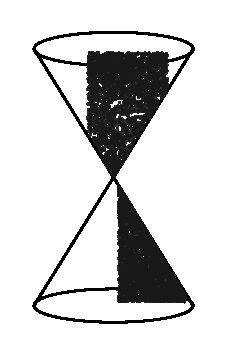
\includegraphics[width=0.72\textwidth]{fig_4.4.pdf}
\caption*{图 4.4\quad “费米点”附近的态密度按 $N(\xi) \propto |\xi|^{d-1}$ 的方式趋于零。}
\end{figure}

\subsection*{问题 4.2.1}

证明式 (4.2.7) 与式 (4.2.9)。

\subsection*{问题 4.2.2}

由式 (4.2.6) 证明式 (4.2.8)。

\subsection*{问题 4.2.3}

证明式 (4.2.10)。

\subsection*{问题 4.2.4}

就 $W = c_{k_{1}}c_{k_{2}}^{\dagger}c_{k_{3}}c_{k_{4}}^{\dagger}$ 与 $W = c_{k_{1}}c_{k_{2}}c_{k_{3}}^{\dagger}c_{k_{4}}^{\dagger}$ 两种情形，验证 Wick 定理的正确性。

\subsection{等空间格林函数与隧穿}

\begin{keypoints}
\item 格林函数在长时间上的代数衰减与跨费米面的无能隙激发相关。
\end{keypoints}

实时空中的格林函数由 $\mathrm{i}G(t, \pmb{x}_{1}, \pmb{x}_{2}) = \langle T(c(t, \pmb{x}_{1})c(0, \pmb{x}_{2})\rangle$ 给出。对于平移不变的系统（例如自由费米子系统），格林函数只依赖于 $\pmb{x}_{1} - \pmb{x}_{2}$，即 $G(t, \pmb{x}_{1}, \pmb{x}_{2}) = G(t, \pmb{x}_{1} - \pmb{x}_{2})$。对于自由费米子系统，我们有 $G(t, \pmb{x}) = \int \frac{\mathrm{d}^{d}\pmb{k}}{(2\pi)^{d}}G(t, \pmb{k})$。当 $\pmb{x} = 0$ 时（或者说，当 $\langle T(c(\pmb{x}_{1}, t_{1})c^{\dagger}(\pmb{x}_{2}, t_{2}))\rangle$ 中的费米算符位于等空间点（equal-space point）$\pmb{x}_{1} = \pmb{x}_{2}$ 上时），我们有
\begin{equation*}
\mathrm{i}G(t, 0) = \int \frac{\mathrm{d}^{d}\pmb{k}}{(2\pi)^{d}}\left(+\Theta(t)\Theta(\xi_{\pmb{k}})\mathrm{e}^{-\mathrm{i}t\xi_{\pmb{k}}} - \Theta(-t)\Theta(-\xi_{\pmb{k}})\mathrm{e}^{-\mathrm{i}t\xi_{\pmb{k}}}\right)
\end{equation*}

\begin{figure}[H]
\centering
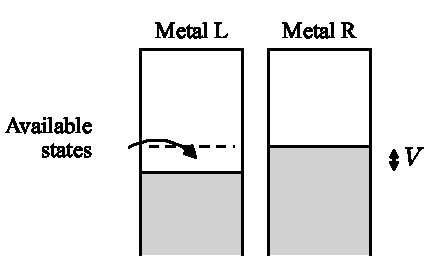
\includegraphics[width=0.72\textwidth]{fig_4.5.pdf}
\caption*{图 4.5\quad 可用于隧穿的态的数目正比于 $V$。}
\end{figure}

上式可以通过引入态密度（density of states，单位体积单位能量内态的数目）
\begin{equation*}
N(\epsilon) = \int \frac{\mathrm{d}^{d}\pmb{k}}{(2\pi)^{d}}\,\delta(\epsilon_{\pmb{k}} - \epsilon)
\end{equation*}
来计算，其中
\begin{align*}
N(\epsilon) &= \sqrt{\frac{m}{2\pi^{2}\epsilon}} && \text{当 } d = 1\\
N(\epsilon) &= \frac{m}{2\pi} && \text{当 } d = 2\\
N(\epsilon) &= \frac{m\sqrt{2m\epsilon}}{2\pi^{2}} && \text{当 } d = 3 \tag{4.2.12}
\end{align*}
在 $T = 0$ 且 $t$ 很大时，只有 $\epsilon = E_{F}$ 附近的 $N(\epsilon)$ 才是重要的。于是我们可以假定 $N(\epsilon) = N(E_{F})$ 为常数。代入 $\int \mathrm{d}^{d}\pmb{k}/(2\pi)^{d} = \int \mathrm{d}\xi\, N(\xi + E_{F})$ 后，对于大的 $t$，我们求得
\begin{equation*}
G(t, 0) = -\frac{N(E_{F})}{t - \mathrm{i}0^{+}\operatorname{sgn}(t)}
\end{equation*}
长时间上的代数关联是被占据态的态密度中不连续性的后果。如果态密度按 $N(\epsilon) \propto |\epsilon - E_{F}|^{g}$ 的方式趋于零（见图 4.4），则长时间关联将衰减得更快（假定 $g > 0$）：
\begin{equation*}
G(t, 0) \propto -\mathrm{i}\operatorname{sgn}(t)\,\mathrm{e}^{-\mathrm{i}\frac{\pi}{2}(1+g)}\frac{1}{|t|^{1+g}}
\end{equation*}

费米子格林函数只有在实验中能够测量才有意义。为了考察如何在实验中测量费米子格林函数，考虑两个态密度为 $N_{R,L}(\xi) \propto |\xi|^{g_{R,L}}$ 的金属之间的隧穿（tunneling）。（注意，对普通金属有 $g_{R,L} = 0$。）假定隧穿哈密顿量为
\begin{equation*}
H_{T} = \Gamma(\mathrm{e}^{\mathrm{i}Vt}c_{R}^{\dagger}c_{L} + \text{h.c.})
\end{equation*}
则从左到右的隧穿电流为（见式 (3.7.15)）
\begin{align*}
\langle j_{T}\rangle(t) &= -\Gamma^{2}\int^{t}\mathrm{d}t'\left(\mathrm{e}^{\mathrm{i}V(t-t')}\left\langle [I(t), I^{\dagger}(t')]\right\rangle + \text{h.c.}\right)\\
&= (-\mathrm{i}\Gamma^{2}D^{\beta}(V) + \text{h.c.}) = 2\Gamma^{2}\mathrm{Im}D^{\beta}(V)
\end{align*}
其中 $I(t) = c_{R}^{\dagger}(t,0)c_{L}(t,0)$ 是隧穿算符。隧穿算符 $I(t) = c_{R}^{\dagger}(t,0)c_{L}(t,0)$ 的关联为（设 $t > 0$ 且 $T = 0$）
\begin{align*}
\left\langle I(t)I^{\dagger}(0)\right\rangle &= \left\langle c_{L}(t,0)c_{L}^{\dagger}(0,0)\right\rangle\left\langle c_{R}^{\dagger}(t,0)c_{R}(0,0)\right\rangle\\
&= -G_{L}(t,0)(-)G_{R}(-t,0)\\
&\propto \mathrm{e}^{-\mathrm{i}\frac{\pi}{2}(2+g_{R}+g_{L})}\frac{1}{t^{2+g_{R}+g_{L}}}
\end{align*}
我们看到，隧穿实验测量的是结两侧等空间格林函数的乘积。上述关联与两个 $(1+1)$ 维相互作用玻色系统之间隧穿算符的关联具有相同的形式。重复 3.7.4 节中的计算，我们求得隧穿电流为
\begin{equation*}
I \propto V^{1+g_{R}+g_{L}} = V \times V^{g_{R}} \times V^{g_{L}}
\end{equation*}
当 $g_{L} = g_{R} = 0$ 时，很容易看出可用于隧穿的态的数目正比于 $V$（图 4.5），因而 $I \propto V$。当 $g_{L}$ 与 $g_{R}$ 不为零时，可用的态将受到相应的压制，因而隧穿电流被因子 $V^{g_{R}} \times V^{g_{L}}$ 压低。

我们想强调，隧穿直接测量的是费米子格林函数。虽然上面我们只讨论了自由费米子系统，这些结果同样适用于相互作用的费米子。设想相互作用改变了费米子格林函数中的长时间衰减指数 $g$；那么这一改变就可以通过隧穿实验测出。

\subsection{费米子谱函数}

\begin{keypoints}
\item 费米子格林函数的谱函数（spectral function）。
\item 费米子格林函数（或更确切地说，费米子谱函数的交叠）可以在隧穿实验中测量。
\end{keypoints}

对相互作用的电子，$G_{L,R}(t,0)$ 要更复杂。为了理解两个相互作用费米子系统之间的隧穿，引入费米子格林函数的谱表示（spectral representation）是有用的：\footnote{如果取 $\eta = 1$，下面的讨论同样适用于玻色算符。}
\begin{equation*}
\mathrm{i}G^{\beta}(t,0) = \left\{\begin{array}{ll}
\int \mathrm{d}\omega\, A_{+}^{0}(\omega)\mathrm{e}^{-\mathrm{i}\omega t}, & \text{当 } t > 0\\
\eta \int \mathrm{d}\omega\, A_{-}^{0}(\omega)\mathrm{e}^{-\mathrm{i}\omega t}, & \text{当 } t < 0
\end{array}\right.
\end{equation*}
其中 $A_{+,-}^{0}(\omega)$ 为下列谱函数：
\begin{equation*}
A_{+}^{0}(\nu) = \sum_{m,n}\delta[\nu - (\epsilon_{m} - \epsilon_{n})]\langle \psi_{n}|c(\pmb{x})|\psi_{m}\rangle\langle \psi_{m}|c^{\dagger}(\pmb{x})|\psi_{n}\rangle\frac{\mathrm{e}^{-\epsilon_{n}\beta}}{Z}
\end{equation*}
\begin{equation*}
A_{-}^{0}(\nu) = \sum_{m,n}\delta[\nu + (\epsilon_{m} - \epsilon_{n})]\langle \psi_{n}|c^{\dagger}(\pmb{x})|\psi_{m}\rangle\langle \psi_{m}|c(\pmb{x})|\psi_{n}\rangle\frac{\mathrm{e}^{-\epsilon_{n}\beta}}{Z}
\end{equation*}
并且，对费米子算符 $\eta = -1$（如果我们想为玻色子格林函数引入谱表示，则取 $\eta = 1$）。我们也可以在动量空间中引入谱函数：
\begin{equation*}
\mathrm{i}G^{\beta}(t,\pmb{k}) = \left\{\begin{array}{ll}
\int \mathrm{d}\omega\, A_{+}(\omega,\pmb{k})\mathrm{e}^{-\mathrm{i}\omega t} & \text{当 } t > 0\\
\eta \int \mathrm{d}\omega\, A_{-}(\omega,\pmb{k})\mathrm{e}^{-\mathrm{i}\omega t} & \text{当 } t < 0
\end{array}\right. \tag{4.2.13}
\end{equation*}
其中
\begin{equation*}
A_{+}(\nu,\pmb{k}) = \sum_{m,n}\delta[\nu - (\epsilon_{m} - \epsilon_{n})]\langle \psi_{n}|c_{\pmb{k}}|\psi_{m}\rangle\langle \psi_{m}|c_{\pmb{k}}^{\dagger}|\psi_{n}\rangle\frac{\mathrm{e}^{-\epsilon_{n}\beta}}{Z}
\end{equation*}
\begin{equation*}
A_{-}(\nu,\pmb{k}) = \sum_{m,n}\delta[\nu + (\epsilon_{m} - \epsilon_{n})]\langle \psi_{n}|c_{\pmb{k}}^{\dagger}|\psi_{m}\rangle\langle \psi_{m}|c_{\pmb{k}}|\psi_{n}\rangle\frac{\mathrm{e}^{-\epsilon_{n}\beta}}{Z}
\end{equation*}
我们看到
\begin{equation*}
A_{\pm}^{0}(\omega) = \mathcal{V}^{-1}\sum_{\pmb{k}}A_{\pm}(\omega,\pmb{k})
\end{equation*}
由定义我们还看到，$A_{+,-}^{0}$ 与 $A_{+,-}$ 是实的且为正。在 $\omega$--$\pmb{k}$ 空间中，我们求得
\begin{align*}
G_{+}^{\beta}(\omega,\pmb{k}) &\equiv \int \mathrm{d}t\,\Theta(t)G^{\beta}(t,\pmb{k})\mathrm{e}^{\mathrm{i}\omega t} = \int \mathrm{d}\nu\,\frac{A_{+}(\nu,\pmb{k})}{\omega - \nu + \mathrm{i}0^{+}}\\
G_{-}^{\beta}(\omega,\pmb{k}) &\equiv \int \mathrm{d}t\,\Theta(-t)G^{\beta}(t,\pmb{k})\mathrm{e}^{\mathrm{i}\omega t} = -\eta \int \mathrm{d}\nu\,\frac{A_{-}(\nu,\pmb{k})}{\omega - \nu - \mathrm{i}0^{+}} \tag{4.2.14}
\end{align*}
动量空间中的谱函数 $A_{+,-}(\nu,\pmb{k})$ 完全决定了格林函数。

\begin{figure}[H]
\centering
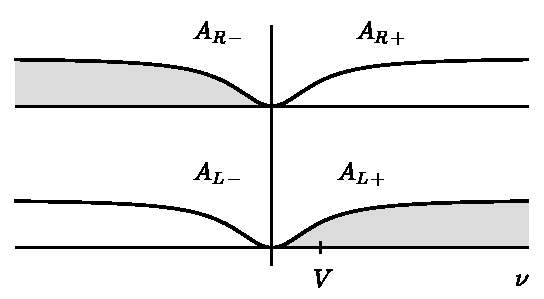
\includegraphics[width=0.72\textwidth]{fig_4.6.pdf}
\caption*{图 4.6\quad 谱函数及其交叠。}
\end{figure}

响应函数 $\langle [I(t), I^{\dagger}(0)]\rangle$ 可以用 R、L 两种金属中的谱函数表出。对 $t > 0$，我们求得
\begin{align*}
&\left\langle [I(t), I^{\dagger}(0)]\right\rangle\\
={}& \left\langle c_{L}(t,0)c_{L}^{\dagger}(0,0)\right\rangle\left\langle c_{R}^{\dagger}(t,0)c_{R}(0,0)\right\rangle - \left\langle c_{L}^{\dagger}(0,0)c_{L}(t,0)\right\rangle\left\langle c_{R}(0,0)c_{R}^{\dagger}(t,0)\right\rangle\\
={}& (\mathrm{i}G_{L}(t))(-\mathrm{i}G_{R}(-t)) - (-\mathrm{i}G_{L}(-t))^{*}(\mathrm{i}G_{R}(t))^{*} \tag{4.2.15}\\
={}& -\int \mathrm{d}\omega_{L}\mathrm{d}\omega_{R}\left(A_{L+}^{0}(\omega_{L})A_{R-}^{0}(\omega_{R}) - A_{L-}^{0}(\omega_{L})A_{R+}^{0}(\omega_{R})\right)\mathrm{e}^{\mathrm{i}(\omega_{R}-\omega_{L})t}
\end{align*}
于是，响应函数 $\mathrm{i}D^{\beta}(t) = \Theta(t)[I(t), I^{\dagger}(0)]$ 在 $\omega$ 空间中由下式给出：
\begin{align*}
D^{\beta}(\omega) = {}& \int \mathrm{d}t\, D^{\beta}(t)\mathrm{e}^{\mathrm{i}\omega t} \tag{4.2.16}\\
={}& \int \mathrm{d}\omega_{L}\mathrm{d}\omega_{R}\,\frac{A_{L+}^{0}(\omega_{L})A_{R-}^{0}(\omega_{R}) - A_{L-}^{0}(\omega_{L})A_{R+}^{0}(\omega_{R})}{\omega - \omega_{L} + \omega_{R} + \mathrm{i}0^{+}}
\end{align*}
从左到右的隧穿电流由虚部确定：
\begin{align*}
\langle j_{T}\rangle(t) ={}& 2\Gamma^{2}\mathrm{Im}D^{\beta}(V)\\
={}& 2\pi\Gamma^{2}\int \mathrm{d}\nu\left(A_{L-}^{0}(\nu)A_{R+}^{0}(\nu - V) - A_{L+}^{0}(\nu)A_{R-}^{0}(\nu - V)\right) \tag{4.2.17}
\end{align*}
在零温下，$A_{+}(\omega)$ 仅当 $\omega > 0$ 时非零，而 $A_{-}(\omega)$ 仅当 $\omega < 0$ 时非零。因此，两式中只有一项有贡献，取决于 $V$ 的符号（见图 4.6）。该贡献是隧穿结（tunneling junction）两侧谱函数的一个交叠积分（overlap integral）。

对自由费米子，由虚时格林函数 (4.2.9) 出发，我们求得（见式 (2.2.37)）
\begin{equation*}
A_{-}(\omega,\pmb{k}) = n_{F}(\xi_{\pmb{k}})\delta(\omega - \xi_{\pmb{k}}), \qquad A_{+}(\omega,\pmb{k}) = (1 - n_{F}(\xi_{\pmb{k}}))\delta(\omega - \xi_{\pmb{k}})
\end{equation*}
（把上式代入式 (4.2.14)，便可恢复有限温度下由式 (4.2.5) 给出的自由电子格林函数。）对 $\pmb{k}$ 积分后，我们得到
\begin{equation*}
A_{-}^{0}(\omega) = n_{F}(\omega)N(\omega + E_{F}), \qquad A_{+}^{0}(\omega) = (1 - n_{F}(\omega))N(\omega + E_{F}) \tag{4.2.18}
\end{equation*}
隧穿电流为
\begin{align*}
\langle j_{T}\rangle(t) = {}& 2\pi\Gamma^{2}\int \mathrm{d}\nu \left[(1 - n_{F}(\nu))N_{L}(\nu + E_{F})n_{F}(\nu - V)N_{R}(\nu - V + E_{F})\right.\\
&\left.- n_{F}(\nu)N_{L}(\nu + E_{F})(1 - n_{F}(\nu - V))N_{R}(\nu - V + E_{F})\right]\\
\approx {}& 2\pi\Gamma^{2}N_{L}(E_{F})N_{R}(E_{F})\int \mathrm{d}\nu\left(n_{F}(\nu - V) - n_{F}(\nu)\right)
\end{align*}
这是一个非常简单的结果，可以直接用二阶微扰论得到。

\subsection*{问题 4.2.5}

计算 $d = 1$ 维时实时空中的编时费米子格林函数在 $(t, x) \to \infty$ 极限下的结果（但 $t/x$ 任意）。在 $t/x \to 0$ 与 $t/x \to \infty$ 两个极限下检验你的结果。

\subsection*{问题 4.2.6}

两个相同的 $d = 1$ 维自由费米子系统在位于 $x = 0$ 和 $x = a$ 的两点处连接。隧穿哈密顿量为
\begin{equation*}
H_{T} = \Gamma\left[\left[c_{L}(0)c_{R}^{\dagger}(0) + c_{L}(a)c_{R}^{\dagger}(a)\right] + \text{h.c.}\right]
\end{equation*}
利用上一题的结果，求作为 $a$ 的函数的隧穿电导。

\subsection*{问题 4.2.7}

证明有限温度下的谱求和规则（spectral sum rule）
\begin{equation*}
\int \mathrm{d}\omega \left(A_{+}(\omega,\pmb{k}) + A_{-}(\omega,\pmb{k})\right) = 1
\end{equation*}
（提示：利用 $\{c_{k}, c_{k}^{\dagger}\} = 1$。）

\subsection*{问题 4.2.8}

\textbf{平行二维电子系统之间的隧穿}（Eisenstein et al., 1991）：考虑二维的两个相同费米子系统，由一个竖直面积隧穿结（vertical area tunneling junction）连接，该结保持二维动量守恒（见图 4.7(a)）。隧穿哈密顿量具有如下形式：

\begin{figure}[H]
\centering
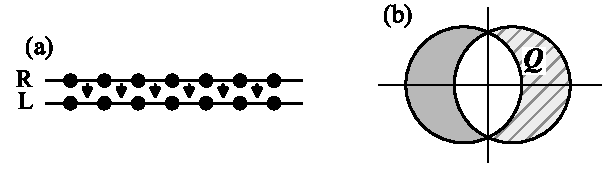
\includegraphics[width=0.72\textwidth]{fig_4.7.pdf}
\caption*{图 4.7\quad (a) 竖直面积隧穿结；(b) 两张发生错移的费米面。}
\end{figure}

\begin{equation*}
H_{T} = A \sum_{\pmb{k}}\left[c_{L\pmb{k}}c_{R\pmb{k}}^{\dagger} + \text{h.c.}\right]
\end{equation*}
在没有平行于二维层的磁场时，两层中的费米子具有相同的色散关系 $\epsilon_{\pmb{k}}$。当存在平行于二维层的磁场 $B$ 时，两层中费米子的动量彼此相对错移（见图 4.7(b)），两层中的色散变为
\begin{equation*}
\epsilon_{R\pmb{k}} = \epsilon_{\pmb{k} - \frac{1}{2}\pmb{Q}}, \qquad \epsilon_{L\pmb{k}} = \epsilon_{\pmb{k} + \frac{1}{2}\pmb{Q}}
\end{equation*}
其中 $Q \propto B$ 且 $\pmb{Q} \cdot \pmb{B} = 0$。

\begin{enumerate}
\item 证明：对自由费米子，当 $B = 0$ 且电压有限（$V \neq 0$）时，有限温度下的隧穿电流为零。
\item 假定由于相互作用，费米子的谱函数具有如下形式：
\begin{equation*}
A_{+}(\omega,\pmb{k}) = (1 - n_{F}(\omega))\frac{\pi^{-1}\Gamma}{(\omega - \xi_{\pmb{k}})^{2} + \Gamma^{2}}, \qquad A_{-}(\omega,\pmb{k}) = n_{F}(\omega)\frac{\pi^{-1}\Gamma}{(\omega - \xi_{\pmb{k}})^{2} + \Gamma^{2}}
\end{equation*}
其中 $\Gamma \ll E_{F}$ 是一个衰变率（注意上述 $A_{\pm}$ 满足式 (2.2.28)）。求温度小而非零（$T \ll E_{F}$）时隧穿电流的表达式。
\item 当 $B = 0$ 时，在 $T \to 0$ 与 $T \gg \Gamma$ 极限下，隧穿电导对温度的依赖关系是什么？估算 $T = 0$ 时单位面积的隧穿电导。
\item 假定零温下 $B = 0$ 时的隧穿电导为 $\sigma_{0}$，试以 $\sigma_{0}$ 估算有限 $Q$ 下的隧穿电导 $\sigma_{Q}$。当 $Q$ 靠近 0 以及靠近 $2k_{F}$ 时，$\sigma_{Q}$ 的行为如何？
\end{enumerate}

\subsection{等时格林函数与费米面的形状}

\begin{keypoints}
\item 长距离上的代数衰减与动量空间中费米子占据数的锐利特征（不连续性）相关。
\end{keypoints}

我们转向等时（equal-time）格林函数。等时关联完全由基态波函数决定。从定义也容易看出，$G^{\beta}(0^{+},\pmb{x})$ 与 $G^{\beta}(-0^{+},\pmb{x})$ 相差一个反对易子（若算符是玻色型的，则为对易子）的平均：
\begin{equation*}
G^{\beta}(0^{+},\pmb{x}) - G^{\beta}(-0^{+},\pmb{x}) = \left\langle \{c(\pmb{x}), c^{\dagger}(0)\}\right\rangle = \delta(\pmb{x})
\end{equation*}
这里我们想选定一个方向 $\hat{\pmb{x}}$，考察 $G(\pm 0^{+}, x\hat{\pmb{x}})$ 在大 $x$ 下的行为。

在 $T = 0$ 时，$G(-0^{+},\pmb{x})$ 可以写为
\begin{equation*}
\mathrm{i}G(-0^{+},\pmb{x}) = -\int \frac{\mathrm{d}^{d}\pmb{k}}{(2\pi)^{d}}\, n_{F}(\xi_{\pmb{k}})\mathrm{e}^{\mathrm{i}\pmb{k}\cdot\pmb{x}} = -\int_{-\infty}^{+\infty}\mathrm{d}k\, \tilde{N}(k,\hat{\pmb{x}})\mathrm{e}^{\mathrm{i}k|\pmb{x}|}
\end{equation*}
其中
\begin{equation*}
\tilde{N}(k,\hat{\pmb{x}}) = \int \frac{\mathrm{d}^{d}\pmb{k}}{(2\pi)^{d}}\,\Theta(-\xi_{\pmb{k}})\delta(k - \pmb{k}\cdot\hat{\pmb{x}})
\end{equation*}
它可以视为动量空间中被占据态的密度。

\begin{figure}[H]
\centering
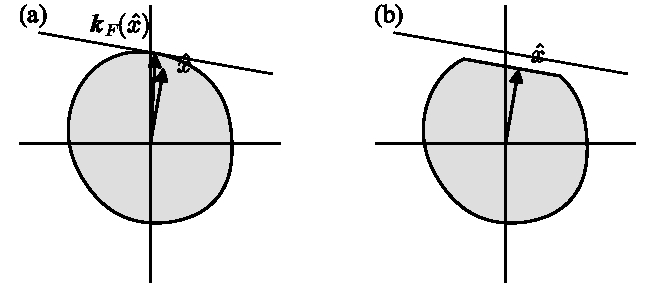
\includegraphics[width=0.72\textwidth]{fig_4.8.pdf}
\caption*{图 4.8\quad (a) $\pmb{k}_{F}(\hat{\pmb{x}})$ 的定义，其中的直线与 $x$ 垂直。(b) 带有一块平坦区域的费米面。}
\end{figure}

从图 4.8(a) 我们看到，一般地，$\tilde{N}(k,\hat{\pmb{x}})$ 在 $k = \pmb{k}_{F}(\hat{\pmb{x}})\cdot\hat{\pmb{x}}$ 与 $k = \pmb{k}_{F}(-\hat{\pmb{x}})\cdot\hat{\pmb{x}}$ 处含有两个奇点：
\begin{align*}
\tilde{N}(k,\hat{\pmb{x}}) ={}& c_{+}\Theta(\pmb{k}_{F}(\hat{\pmb{x}})\cdot\hat{\pmb{x}} - k)\,|\pmb{k}_{F}(\hat{\pmb{x}})\cdot\hat{\pmb{x}} - k|^{(d-1)/2}\\
&+ c_{-}\Theta(-\pmb{k}_{F}(-\hat{\pmb{x}})\cdot\hat{\pmb{x}} + k)\,\left|-\pmb{k}_{F}(-\hat{\pmb{x}})\cdot\hat{\pmb{x}} + k\right|^{(d-1)/2}
\end{align*}
（例如在一维情形，$\tilde{N}(k,\hat{\pmb{x}})$ 有两个不连续的台阶。）这两个奇点导致如下代数长程的等时关联：
\begin{equation*}
\mathrm{i}G(-0^{+},\pmb{x})\big|_{\pmb{x}\to\infty} \sim \left(c_{+}\mathrm{e}^{\mathrm{i}\pmb{k}_{F}(\hat{\pmb{x}})\cdot\pmb{x}}\mathrm{e}^{-\mathrm{i}\frac{\pi(d+1)}{4}} + c_{-}\mathrm{e}^{\mathrm{i}\pmb{k}_{F}(-\hat{\pmb{x}})\cdot\pmb{x}}\mathrm{e}^{+\mathrm{i}\frac{\pi(d+1)}{4}}\right)\frac{1}{|\pmb{x}|^{(d+1)/2}}
\end{equation*}
对球形的费米面，我们有
\begin{equation*}
\mathrm{i}G(-0^{+},\pmb{x})\big|_{\pmb{x}\to\infty} \sim \cos\left(k_{F}|\pmb{x}| - \frac{\pi(d+1)}{4}\right)\frac{1}{|\pmb{x}|^{(d+1)/2}}
\end{equation*}
如果费米面包含一块平坦区域（见图 4.8(b)），那么 $\tilde{N}(k,\hat{\pmb{x}})$ 在相应方向上会有一个不连续台阶。在该方向上，$G(-0^{+},\pmb{x})$ 将具有较慢的代数衰减，其衰减幂次与一维系统的相同：
\begin{equation*}
\mathrm{i}G(-0^{+},\pmb{x})\big|_{\pmb{x}\to\infty} \sim -\mathrm{i}\,\mathrm{e}^{\mathrm{i}\pmb{k}_{F}(\hat{\pmb{x}})\cdot x}\frac{1}{|\pmb{x}|}
\end{equation*}

\section{两体关联函数与线性响应}

\begin{keypoints}
\item 我们可以由两体关联函数计算线性响应。这使我们能够计算许多可测量的量。
\item 两体关联函数揭示自由费米子基态的许多潜在不稳定性。
\end{keypoints}

两体关联函数（two-body correlation functions）是最重要的一类关联。实验中测量的大多数物理量都直接与两体关联相关。这些物理量包括电导与热导、中子与光散射截面、弹性常数、介电常数、磁化率等等（见 3.7.2 节）。下面我们将讨论无自旋自由费米子系统的两体关联。

\subsection{密度--密度关联函数}

我们首先考虑两体关联中的一种——密度关联函数
\begin{equation*}
\mathrm{i}P^{00}(t,\pmb{x}) = \langle T(\rho(t,\pmb{x})\rho(0))\rangle
\end{equation*}
其中
\begin{equation*}
\rho(t,\pmb{x}) = c^{\dagger}(t,\pmb{x})c(t,\pmb{x}).
\end{equation*}
密度关联函数与压缩率以及中子/光散射相关。为了计算 $P^{00}(t,\pmb{x})$，我们可以对自由费米子算符应用 Wick 定理，如下：

\begin{figure}[H]
\centering
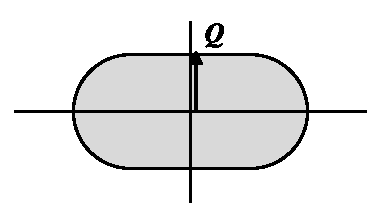
\includegraphics[width=0.72\textwidth]{fig_4.9.pdf}
\caption*{图 4.9\quad 具有嵌套波矢 $Q$ 的嵌套费米面。}
\end{figure}

\begin{align*}
\mathrm{i}P^{00}(t,\pmb{x}) ={}& \left\langle T[c^{\dagger}(t + 0^{+},\pmb{x})c(t,\pmb{x})c^{\dagger}(0^{+})c(0)]\right\rangle\\
={}& \rho_{0}^{2} - \mathrm{i}G(-t,-\pmb{x})\,iG(t,\pmb{x})
\end{align*}
利用前面已算出的费米子格林函数，我们发现，在 $t = 0$ 极限下，对于球形费米面，有
\begin{equation*}
\mathrm{i}P^{00}(0,\pmb{x}) = \rho_{0}^{2} + C\left(1 - \sin\left(2k_{F}|\pmb{x}| - \frac{\pi(d+1)}{2}\right)\right)\frac{1}{|\pmb{x}|^{(d+1)}}
\end{equation*}
对图 4.9 中的嵌套费米面（nested Fermi surface），我们有
\begin{equation*}
\mathrm{i}P^{00}(0,\pmb{x}) = \rho_{0}^{2} + C[1 + \sin(Q|\pmb{x}|)]\frac{1}{|\pmb{x}|^{2}}
\end{equation*}
其中 $x \| Q$。

我们知道，在晶体中，密度关联会一直振荡而没有任何衰减，即 $\mathrm{i}P^{00}(0,\pmb{x}) = \rho_{0}^{2} + C[1 + \sin(Q|\pmb{x}|)]$。振荡部分代表了有序晶体中的长程序。我们看到，自由的费米子基态没有长程晶体序，但它具有“代数长程”晶体序，对嵌套费米面尤其如此（见图 4.10）。在某种意义上，嵌套的自由费米子系统正处于成为晶体的边缘。我们将在本章后面看到，只要开启一个小的相互作用，“代数长程”晶体序就可以被提升为长程晶体序。
为了得到自由费米子的线性响应，我们需要计算密度响应函数 $\Pi^{00}$。在 $t$--$\pmb{k}$ 空间中，密度响应函数可以
用 Wick 定理如下求出：
\begin{align*}
\mathrm{i}\Pi^{00}(t,\pmb{k}) &= \Theta(t)\mathcal{V}^{-1}\left\langle \Big[\sum_{\pmb{q}}\big(c^{\dagger}_{\pmb{q}}c_{\pmb{q}+\pmb{k}}\big)(t),\, \sum_{\pmb{q}'}\big(c^{\dagger}_{\pmb{q}'}c_{\pmb{q}'-\pmb{k}}\big)(0)\Big] \right\rangle \tag{4.3.1}\\
&= \Theta(t)\mathcal{V}^{-1}\sum_{\pmb{q}}\left(1-n_F(\xi_{\pmb{q}+\pmb{k}})\right)n_F(\xi_{\pmb{q}})\,\mathrm{e}^{-\mathrm{i}t(\xi_{\pmb{q}+\pmb{k}}-\xi_{\pmb{q}})}\\
&\quad -\, \Theta(t)\mathcal{V}^{-1}\sum_{\pmb{q}}\left(1-n_F(\xi_{\pmb{q}})\right)n_F(\xi_{\pmb{q}+\pmb{k}})\,\mathrm{e}^{+\mathrm{i}t(\xi_{\pmb{q}}-\xi_{\pmb{q}+\pmb{k}})}
\end{align*}
\begin{figure}[H]
\centering
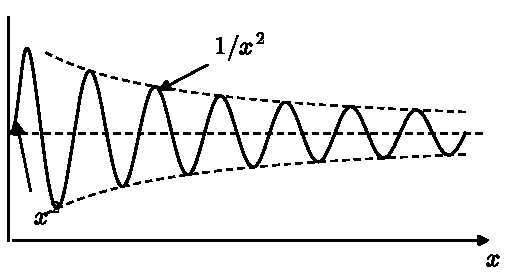
\includegraphics[width=0.72\textwidth]{fig_4.10.pdf}
\caption*{图 4.10\quad 嵌套费米面的密度关联 $\mathrm{i}P^{00}(0,\boldsymbol{x})$ 中的“代数长程”晶体序。}
\end{figure}

只有当 $\pmb{q}'=\pmb{q}+\pmb{k}$ 时，上述平均才不为零。在第一项中，我们在 $\pmb{q}+\pmb{k}$ 处产生一个费米子、在 $\pmb{q}$ 处湮灭一个费米子，这给出因子 $\left(1-n_F(\xi_{\pmb{q}+\pmb{k}})\right)n_F(\xi_{\pmb{q}})$。第二项具有类似的结构，其中我们在 $\pmb{q}$ 处产生一个费米子、在 $\pmb{q}+\pmb{k}$ 处湮灭一个费米子。

在 $\omega$–$\pmb{k}$ 空间中，我们有
\begin{equation*}
\Pi^{00}(\omega,\pmb{k}) = \mathcal{V}^{-1}\sum_{\pmb{q}}\left( \frac{\left(1-n_F(\xi_{\pmb{q}+\pmb{k}})\right)n_F(\xi_{\pmb{q}})}{\omega-\xi_{\pmb{q}+\pmb{k}}+\xi_{\pmb{q}}+\mathrm{i}0^{+}} - \frac{\left(1-n_F(\xi_{\pmb{q}})\right)n_F(\xi_{\pmb{q}+\pmb{k}})}{\omega+\xi_{\pmb{q}}-\xi_{\pmb{q}+\pmb{k}}+\mathrm{i}0^{+}} \right)
\end{equation*}

$\Pi^{00}(\omega,\pmb{k})$ 的虚部仅在 $(\omega,\pmb{k})$ 对应于粒子–空穴激发的能量–动量时才不为零（见图 4.11）。这一特征出现在任何二体关联函数之中，包括流关联与自旋关联。

在 $|\pmb{k}|\ll k_F$ 且 $T$ 有限的极限下，我们有
\begin{equation*}
\Pi^{00}(\omega,\pmb{k}) = -\int \frac{\mathrm{d}^d\pmb{q}}{(2\pi)^d}\, \frac{\partial n_F}{\partial\xi}\, \frac{\pmb{k}\cdot\pmb{v}}{\omega-\pmb{k}\cdot\pmb{v}+\mathrm{i}0^{+}}
\end{equation*}

其中 $\pmb{v}=\pmb{q}/m$。在 $T\to 0$ 极限下，我们有 $\partial n_F/\partial\xi=-\delta(\xi_{\pmb{k}})$，此时积分变为对费米面的积分。让我们先考虑 $\Pi^{00}(\omega,\pmb{k})$ 的虚部：
\begin{figure}[H]
\centering
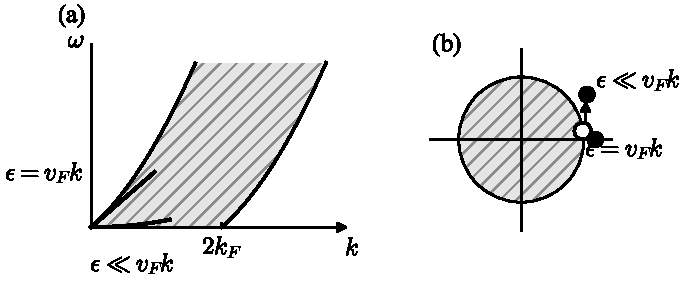
\includegraphics[width=0.72\textwidth]{fig_4.11.pdf}
\caption*{图 4.11\quad (a) 阴影区域表示粒子–空穴激发的能量–动量（对 $d>1$）。$\mathrm{Im}\Pi^{00}(\omega,\boldsymbol{k})$ 仅在阴影区域内不为零。$(\omega,\boldsymbol{k})=(0,0)$ 处的边缘具有斜率 $v_F$，由 (b) 可见。}
\end{figure}
\begin{equation*}
\mathrm{Im}\Pi^{00}(\omega,\pmb{k}) = -\frac{\omega}{v_F k}\, \frac{k_F^{d-1}}{(2\pi)^d v_F} \int \mathrm{d}\Omega\; \pi\delta\left(\frac{\omega}{v_F k}-\cos(\theta)\right)
\end{equation*}

我们发现（见图 4.12）
\begin{equation*}
\mathrm{Im}\,\Pi^{00}(\omega,\pmb{k})
= \left\{
\begin{array}{ll}
-(\omega/v_F k)\left(k_F^2/4\pi v_F\right)\Theta(v_F k-|\omega|), & d=3,\\[1ex]
-(\omega/v_F k)\left(k_F/2\pi v_F\right)\left(1/\sqrt{1-(\omega/v_F k)^2}\right)\Theta(v_F k-|\omega|), & d=2.
\end{array}
\right.
\end{equation*}

为求实部，我们注意到 $\Pi^{00}(\omega,\pmb{k})$ 是一些形如 $1/(\omega-\epsilon+\mathrm{i}0^{+})$ 的函数之和：
\begin{equation*}
\Pi^{00}(\omega,\pmb{k}) = \int \mathrm{d}\epsilon\; \frac{\mathrm{sgn}(\epsilon)A(\epsilon,\pmb{k})}{\omega-\epsilon+\mathrm{i}0^{+}}
\end{equation*}

其中 $A(\epsilon,\pmb{k})$ 是 $\Pi^{00}(\omega,\pmb{k})$ 的谱函数。谱函数与 $\Pi^{00}(\omega,\pmb{k})$ 的虚部直接相关：
\begin{equation*}
\mathrm{Im}\Pi^{00}(\omega,\pmb{k}) = -\mathrm{sgn}(\omega)\pi A(\omega,\pmb{k})
\end{equation*}
\begin{figure}[H]
\centering
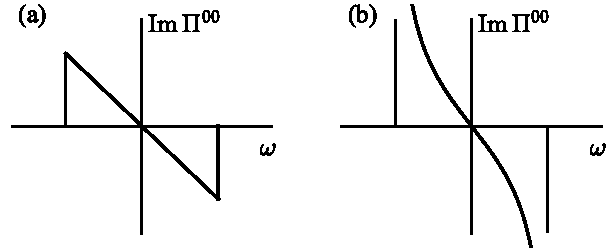
\includegraphics[width=0.72\textwidth]{fig_4.12.pdf}
\caption*{图 4.12\quad 固定小 $k$ 时，(a) $d=3$ 维与 (b) $d=2$ 维的 $\mathrm{Im}\Pi^{00}$。}
\end{figure}

这样，我们可以由虚部 $\mathrm{Im}\Pi^{00}(\omega,\pmb{k})$ 算出实部。我们发现
\begin{equation*}
\Pi^{00}(\omega,\pmb{k})
= \left\{
\begin{array}{ll}
-\dfrac{k_F m}{2\pi^2}\left[1-\dfrac{\omega}{2v_F k}\ln\left|\dfrac{\omega+v_F k}{\omega-v_F k}\right|+\mathrm{i}\dfrac{\pi\omega}{2v_F k}\Theta(v_F k-|\omega|)\right], & \text{对 } d=3,\\[4ex]
-\dfrac{m}{2\pi}\left[1-\dfrac{\omega\Theta(|\omega|-v_F k)}{\sqrt{\omega^2-v_F^2k^2}}+\mathrm{i}\dfrac{\omega\Theta(v_F k-|\omega|)}{\sqrt{v_F^2k^2-\omega^2}}\right], & \text{对 } d=2,\\[4ex]
\dfrac{1}{\pi}\dfrac{v_F k^2}{(\omega+\mathrm{i}0^{+})^2-v_F^2k^2}, & \text{对 } d=1.
\end{array}
\right. \tag{4.3.2}
\end{equation*}

我们注意到，当 $\mathrm{Im}\Pi^{00}(\omega,\pmb{k})$ 在某处（比如说 $\omega_0$）出现不连续跳变时，$\mathrm{Re}\Pi^{00}(\omega,\pmb{k})$ 会在同一处出现对数发散。我们还愿指出，编时关联函数 $P^{00}(\omega,\pmb{k})$ 由同一公式给出，只是虚部多出一个因子 $\mathrm{sgn}(\omega)$。

自由费米子的压缩率决定了势的改变能诱发多大的密度改变。它由 $\chi(\pmb{k})=-\Pi^{00}(0,\pmb{k})$ 给出（在有限波矢 $\pmb{k}$ 处），且在小 $\pmb{k}$ 下与 $\pmb{k}$ 无关。由式 (4.2.12)，我们发现压缩率在所有维度都由费米能处的态密度给出：
\begin{equation*}
\chi(\pmb{k}) = N(E_F)
\end{equation*}

正如所料。由
\begin{equation*}
\sigma(\omega) = -\lim_{\pmb{k}\to 0}\mathrm{Im}\,\frac{\omega}{k^2}\,\Pi^{00}(\omega,\pmb{k})
\end{equation*}

我们也看到光学电导率（optical conductivity）为零（$\sigma(\omega)=0$），只在 $\omega=0$ 处例外。这同样在预料之中。在没有任何相互作用时，均匀的振荡电场无法激发任何粒子–空穴激发，因而不会引起耗散。
\begin{figure}[H]
\centering
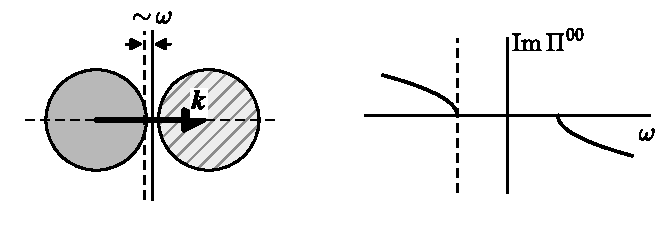
\includegraphics[width=0.72\textwidth]{fig_4.13.pdf}
\caption*{图 4.13\quad $|\boldsymbol{k}|>2k_F$ 时的 $\mathrm{Im}\Pi^{00}$。(a) 中虚线与阴影区域的交截决定了 (b) 中 $\mathrm{Im}\Pi^{00}(\omega,\boldsymbol{k})$ 的值。}
\end{figure}

当 $\omega\ll v_F k$ 时，$\Pi^{00}$ 对所有 $d>1$ 的维度都具有如下形式：
\begin{equation*}
\Pi^{00}(\omega,\pmb{k}) = -N(E_F)\left(1+\mathrm{i}C_d\frac{\omega}{v_F k}\right)
\end{equation*}

其中 $d=2$ 时 $C_2=1$，$d=3$ 时 $C_3=\pi/2$。我们看到，当 $\pmb{k}\neq 0$ 时，振荡电场会引起耗散。电导率具有形式
\begin{equation*}
\sigma(\omega,\pmb{k}) = N(E_F)C_d\,\frac{\omega^2}{v_F k^3}
\end{equation*}
（在 $\omega\ll v_F k$ 极限下）。

一般而言，当 $\omega$ 小时，$\Pi^{00}(\omega,\pmb{k})$ 是 $\pmb{k}$ 的光滑函数，但在 $\pmb{k}=0$ 与 $|\pmb{k}|=2k_F$ 附近除外（对球形费米面）。我们已经研究了 $\Pi^{00}(\omega,\pmb{k})$ 在 $\pmb{k}=0$ 附近的奇异行为；接下来我们讨论 $\Pi^{00}(\omega,\pmb{k})$ 在 $|\pmb{k}|=2k_F$ 附近的行为。让我们考虑下式的 $T=0$ 极限：
\begin{equation*}
\Pi^{00}(\omega,\pmb{k}) = \int \frac{\mathrm{d}^2\pmb{q}}{(2\pi)^d}\left( \frac{n_F(\xi_{\pmb{q}-\frac{\pmb{k}}{2}})-n_F(\xi_{\pmb{q}+\frac{\pmb{k}}{2}})}{\omega-\left(\xi_{\pmb{q}+\frac{\pmb{k}}{2}}-\xi_{\pmb{q}-\frac{\pmb{k}}{2}}\right)+\mathrm{i}0^{+}} \right)
\end{equation*}

在图 4.13、图 4.14 与图 4.15 中，浅阴影区域内 $n_F(\xi_{\pmb{q}-\frac{\pmb{k}}{2}})-n_F(\xi_{\pmb{q}+\frac{\pmb{k}}{2}})=1$，深阴影区域内 $n_F(\xi_{\pmb{q}-\frac{\pmb{k}}{2}})-n_F(\xi_{\pmb{q}+\frac{\pmb{k}}{2}})=-1$。此外，在 $y$ 轴右侧 $\xi_{\pmb{q}+\frac{\pmb{k}}{2}}-\xi_{\pmb{q}-\frac{\pmb{k}}{2}}>0$，在 $y$ 轴左侧 $\xi_{\pmb{q}+\frac{\pmb{k}}{2}}-\xi_{\pmb{q}-\frac{\pmb{k}}{2}}<0$。虚线是 $\omega=\xi_{\pmb{q}+\frac{\pmb{k}}{2}}-\xi_{\pmb{q}-\frac{\pmb{k}}{2}}$ 的位置。虚线与阴影区域的交截决定了 $\mathrm{Im}\Pi^{00}(\omega,\pmb{k})$ 的值。从图 4.13 与图 4.14 可以清楚地看出，对小 $\omega$：当 $|\pmb{k}|>2k_F$ 时 $\mathrm{Im}\Pi^{00}(\omega,\pmb{k})=0$；当 $|\pmb{k}|<2k_F$ 时 $\mathrm{Im}\Pi^{00}(\omega,\pmb{k})\propto-\omega$；而当 $|\pmb{k}|=2k_F$ 时 $\mathrm{Im}\Pi^{00}(\omega,\pmb{k})\propto-\mathrm{sgn}(\omega)|\omega|^{(d-1)/2}$。这些结果意味着，对 $d>1$，实部 $\mathrm{Re}\Pi^{00}(0,\pmb{k})$ 在 $\pmb{k}=2k_F$ 附近有限。
\begin{figure}[H]
\centering
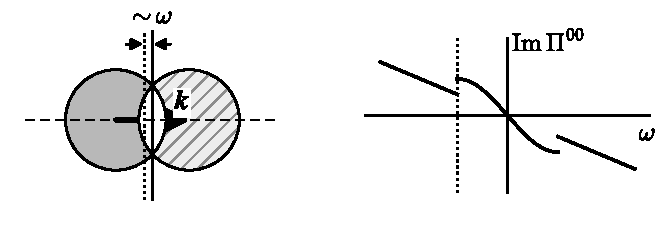
\includegraphics[width=0.72\textwidth]{fig_4.14.pdf}
\caption*{图 4.14\quad $|\boldsymbol{k}|<2k_F$ 时的 $\mathrm{Im}\Pi^{00}$。}
\end{figure}

然而，对嵌套费米面，当 $\pmb{k}$ 等于嵌套波矢 $\pmb{Q}$ 时，$\mathrm{Im}\Pi^{00}(\omega,\pmb{Q})$ 在 $\omega=0$ 处有一个不连续跳变（见图 4.15）。这导致压缩率在嵌套波矢 $\pmb{Q}$ 处出现对数发散：
\begin{equation*}
\chi(\pmb{Q}) \sim N(E_F)\ln\frac{E_F}{\omega}\Big|_{\omega\to 0}
\end{equation*}

在有限温度下，$\omega=0$ 处的不连续跳变被 $T$ 抹平，对数发散被 $T$ 截断：
\begin{equation*}
\chi(\pmb{Q}) \sim N(E_F)\ln\frac{E_F}{T} \tag{4.3.3}
\end{equation*}

我们已经从等时密度关联函数看到，嵌套费米面的基态在嵌套波矢 $\pmb{Q}$ 处含有一种“代数长程”晶体序。这里我们又从零频率密度关联函数看到，打开一个具有波矢 $\pmb{Q}$ 的小周期势会感生出大的密度波。这又是一个与晶体类似的性质：在晶体中，无穷小的周期势就能钉扎晶体并感生出有限的密度波。后面我们将看到，正因为嵌套费米面离晶体序如此之近，打开一个无穷小的相互作用实际上就能导致自发对称性破缺，把费米液体态变成晶体（更确切地说，称为电荷密度波（charge-density-wave，CDW）态）。

\subsection*{问题 4.3.1}

\textbf{一维自由费米子与相互作用玻色子}\quad 计算一维自由费米子系统中大 $(x,t)$ 处的 $T=0$ 编时密度关联 $\langle T\rho(x,t)\rho(0)\rangle$。（提示：利用问题 4.2.5 的结果。）你的结果应当是式 (3.6.2) 中一维相互作用玻色子密度关联的一个特例。确定式 (3.6.2) 中 $\chi$、$v$、$K_n$ 与 $C_n$ 的取值，使之重现自由费米子的编时密度关联。

\subsection*{问题 4.3.2}

对二维自由费米子系统，计算小 $(\omega,k)$ 处虚时中的零温编时密度关联 $\mathcal{P}^{00}(\omega,k)$。完成解析延拓，得到实频率的 $\Pi^{00}$。
\begin{figure}[H]
\centering
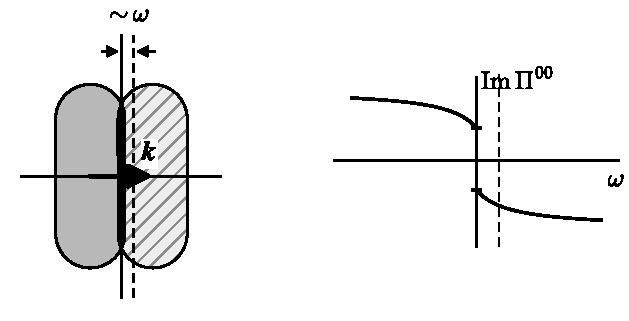
\includegraphics[width=0.72\textwidth]{fig_4.15.pdf}
\caption*{图 4.15\quad 嵌套费米面在 $\boldsymbol{k}=\boldsymbol{Q}$ 处的 $\mathrm{Im}\Pi^{00}$。}
\end{figure}

\subsection{流算符}

\begin{keypoints}
\item 具有一般色散的粒子的流算符。
\end{keypoints}

为了计算流响应函数 $\pi^{ij}$ 与 $\Pi^{ij}$（见 3.7.2 节），我们首先需要知道流算符 $\pmb{j}$ 是什么。我们从密度算符的时间导数 $\mathrm{d}\rho/\mathrm{d}t=\mathrm{d}[c^{\dagger}(\pmb{x},t)c(\pmb{x},t)]/\mathrm{d}t$ 出发，并从守恒定律 $\mathrm{d}\rho/\mathrm{d}t+\pmb{\partial}\cdot\pmb{j}=0$ 得到 $\pmb{j}$。设费米子系统由下式描述：
\begin{equation*}
H = \sum_{\langle ij\rangle}\left(t_{ij}c^{\dagger}_i c_j + h.c.\right)
\end{equation*}

我们发现 $\mathrm{i}\partial_t c=\sum_j(t_{ij}+t^{*}_{ji})c_j$，并且
\begin{equation*}
\partial_t\rho = \sum_j j_{ij}, \qquad j_{ij} = -\mathrm{i}c^{\dagger}_i(t_{ij}+t^{*}_{ji})c_j + \mathrm{i}c^{\dagger}_j(t^{*}_{ij}+t_{ji})c_i
\end{equation*}

这些结果告诉我们，在格点上，流算符由 $j_{ij}$ 给出，它描述每单位时间从格点 $j$ 流向格点 $i$ 的粒子数。这与我们要找的东西非常不同。我们要找的是一个流算符 $\pmb{j}(\pmb{x})$，它是一个矢量，且只依赖一个坐标（而非两个）。这样的流算符对格点模型而言根本不存在。然而，如果 $\pmb{A}$ 是 $\pmb{x}$ 的光滑函数，那么 $\pmb{A}$ 与流之间的耦合只能“看到”流的光滑部分。在这个极限下，即使对格点模型，我们也能找到这样一个类矢量的流算符。

诀窍在于从一个规范化的（gauged）哈密顿量出发。我们先考虑一个连续模型
\begin{equation*}
H = \int \mathrm{d}^d\pmb{x}\; c^{\dagger}(\pmb{x})\epsilon(-\mathrm{i}\partial_{\pmb{x}})c(\pmb{x})
\end{equation*}

其中 $\epsilon(\pmb{k})$ 是费米子的能谱。规范化的哈密顿量为
\begin{equation*}
H = \int \mathrm{d}^d\pmb{x}\; c^{\dagger}(\pmb{x})\epsilon(-\mathrm{i}\partial_i + A_i(\pmb{x}))c(\pmb{x}) \tag{4.3.4}
\end{equation*}

总流算符 $\pmb{J}$ 通过下式得到
\begin{equation*}
J^i(\pmb{x}) = \frac{\delta H}{\delta A_i(\pmb{x})} \tag{4.3.5}
\end{equation*}

这样得到的流算符满足流守恒定律（见问题 4.3.3）。对二次型色散 $\epsilon(\pmb{k})=\pmb{k}^2/2m$，我们有
\begin{equation*}
J^i = \frac{1}{2m}\left[c^{\dagger}(\pmb{x})(-\mathrm{i}\partial_i)c(\pmb{x}) - \left(\mathrm{i}\partial_i c^{\dagger}(\pmb{x})\right)c(\pmb{x})\right] + \frac{1}{m}A_i(\pmb{x})c^{\dagger}(\pmb{x})c(\pmb{x}) \tag{4.3.6}
\end{equation*}

第一项具有 $m^{-1}\pmb{k}\rho$ 的形式。第二项只在 $A_i\neq 0$ 时出现，具有 $m^{-1}A_i\rho$ 的形式。由于 $m^{-1}(k_i+A_i)=v_i$ 是速度，流具有 $v_i\rho$ 的形式，正如所料。

对更一般的色散，流会相当复杂，因为 $\partial_i$ 与 $A_i(\pmb{x})$ 不对易。例如，对具有 $\epsilon(k)=\gamma k^n$ 的一维系统，我们发现如下“讨厌的”形式：
\begin{equation*}
J = \gamma\sum_{m=0}^{n-1}\left[\left(\mathrm{i}\partial_x+A_x\right)^m c^{\dagger}\right]\left[\left(-\mathrm{i}\partial_x+A_x\right)^{n-1-m}c\right]
\end{equation*}

然而，在小动量极限下，我们可以忽略 $\partial_iA_j$ 项，把 $\partial_i$ 与 $A_i(\pmb{x})$ 当作对易的量来处理。在这个极限下，我们得到
\begin{align*}
J^i &= \frac{1}{2m}\left[c^{\dagger}(\pmb{x})v^i(-\mathrm{i}\partial_{\pmb{x}})c(\pmb{x}) + \left(v^i(\mathrm{i}\partial_{\pmb{x}})c^{\dagger}(\pmb{x})\right)c(\pmb{x})\right] \tag{4.3.7}\\
&\quad + \frac{1}{2}A_j(\pmb{x})\left[c^{\dagger}(\pmb{x})K^{ij}(-\mathrm{i}\partial_{\pmb{x}})c(\pmb{x}) + \left[K^{ij}(\mathrm{i}\partial_{\pmb{x}})c^{\dagger}(\pmb{x})\right]c(\pmb{x})\right] + O(\pmb{A}^2)
\end{align*}

其中
\begin{equation*}
v^i(\pmb{k}) = \frac{\partial\epsilon(\pmb{k})}{\partial k_i}, \qquad K^{ij}(\pmb{k}) = \frac{\partial^2\epsilon(\pmb{k})}{\partial k_i\partial k_j}
\end{equation*}

在动量空间中，式 (4.3.7) 可以改写为
\begin{align*}
J^i_{\pmb{q}}(t) &= \sum_{\pmb{k}} c^{\dagger}_{\pmb{k}}c_{\pmb{k}+\pmb{q}}\,\frac{v^i(\pmb{k})+v^i(\pmb{k}+\pmb{q})}{2}\\
&\quad + \mathcal{V}^{-1}\sum_{\pmb{k}\pmb{k}'} c^{\dagger}_{\pmb{k}}c_{\pmb{k}+\pmb{k}'}A^j_{\pmb{q}-\pmb{k}'}\,\frac{K^{ij}(\pmb{k})+K^{ij}(\pmb{k}+\pmb{k}')}{2} \tag{4.3.8}
\end{align*}

其中 $c(\pmb{x},t)=\sum_{\pmb{k}}\mathcal{V}^{-1/2}c_{\pmb{k}}(t)\mathrm{e}^{\mathrm{i}\pmb{k}\cdot\pmb{x}}$，$A_i(\pmb{x},t)=\mathcal{V}^{-1}\sum_{\pmb{k}}A_{i,\pmb{k}}(t)\mathrm{e}^{\mathrm{i}\pmb{k}\cdot\pmb{x}}$，$J^i(\pmb{x},t)=\mathcal{V}^{-1}\sum_{\pmb{k}}J^i_{\pmb{k}}(t)\mathrm{e}^{\mathrm{i}\pmb{k}\cdot\pmb{x}}$。当 $\pmb{A}=0$ 时，流算符变为
\begin{equation*}
j^i_{\pmb{q}}(t) = \sum_{\pmb{k}} c^{\dagger}_{\pmb{k}}(t)c_{\pmb{k}+\pmb{q}}(t)\,\frac{v^i(\pmb{k})+v^i(\pmb{k}+\pmb{q})}{2} \tag{4.3.9}
\end{equation*}

我们想强调，上式仅在小 $\pmb{q}$ 极限下成立。因此，我们也可以把流写成 $j^i_{\pmb{q}}(t)=\sum_{\pmb{k}}c^{\dagger}_{\pmb{k}}c_{\pmb{k}+\pmb{q}}v^i(\pmb{k}+(\pmb{q}/2))$，它在 $O(\pmb{q})$ 精度内与式 (4.3.9) 一致。如果我们把 $\sum_{\pmb{k}}$ 看作对布里渊区（Brillouin zone）的求和，那么式 (4.3.8) 或式 (4.3.9) 就可以看作格点模型的（近似）流算符。

\subsection*{问题 4.3.3}

\textbf{规范不变性与流守恒}
\begin{enumerate}
\item 证明规范化的哈密顿量 (4.3.4) 在规范变换 $c(\pmb{x})\to\mathrm{e}^{-\mathrm{i}\phi(\pmb{x})}c(\pmb{x})$ 与 $A_i(\pmb{x})\to A_i(\pmb{x})+\partial_i\phi(\pmb{x})$ 下不变。
\item 在一维使用规范化的哈密顿量 (4.3.4) 计算 $\partial_t(c^{\dagger}c)$，并证明由式 (4.3.5) 定义的流满足 $\partial_t\rho+\partial_x J=0$。
\end{enumerate}

\subsection*{问题 4.3.4}

求二维自由费米子系统（色散为 $\epsilon_k=\frac{k^2}{2m}+\gamma k^4$）的流算符 $J^i$。

\subsection{流关联函数}

利用式 (4.3.9)，我们现在可以计算流响应函数的第一部分 $\mathrm{i}\pi^{ij}=\langle[j^i,j^j]\rangle$（见式 (3.7.6)）。记住，密度响应函数包含来自 $(\pmb{q},\pmb{q}+\pmb{k})$ 与 $(\pmb{q}+\pmb{k},\pmb{q})$ 处粒子–空穴的两部分贡献。当我们计算流响应函数时，同样有这两部分贡献，只不过两部分都要乘上一个额外的权重因子 $\frac{1}{2}[v^i(\pmb{q})+v^i(\pmb{q}+\pmb{k})]\frac{1}{2}[v^j(\pmb{q})+v^j(\pmb{q}+\pmb{k})]$。因此
\begin{equation*}
\pi^{ij}(\omega,\pmb{k}) = \int \frac{\mathrm{d}^2\pmb{q}}{(2\pi)^d}\, \frac{\left[n_F(\xi_{\pmb{q}})-n_F(\xi_{\pmb{q}+\pmb{k}})\right]\left[v^i(\pmb{q})+v^i(\pmb{q}+\pmb{k})\right]\left[v^j(\pmb{q})+v^j(\pmb{q}+\pmb{k})\right]}{4\left[\omega-(\xi_{\pmb{q}+\pmb{k}}-\xi_{\pmb{q}})+\mathrm{i}0^{+}\right]}
\end{equation*}

在 $\pmb{k}\ll k_F$ 极限下，我们有
\begin{equation*}
\pi^{ij}(\omega,\pmb{k}) = -\int \frac{\mathrm{d}^d\pmb{q}}{(2\pi)^d}\, \frac{\partial n_F}{\partial\xi}\, \frac{\pmb{k}\cdot\pmb{v}(\pmb{q})\left[v^i(\pmb{q})+v^i(\pmb{q}+\pmb{k})\right]\left[v^j(\pmb{q})+v^j(\pmb{q}+\pmb{k})\right]}{4\left[\omega-\pmb{k}\cdot\pmb{v}(\pmb{q})+\mathrm{i}0^{+}\right]}
\end{equation*}

我们先把自己限制在 $\epsilon=\frac{k^2}{2m}$、$T=0$、$d=2$ 的情形。我们已经算出了 $\Pi^{00}$，从而也算出了 $\Pi^{\parallel}$。为计算 $\Pi^{\perp}$，我们取 $\pmb{k}=(k,0)$，于是 $\pi^{\perp}(\omega,k)=\pi^{22}(k\hat{\pmb{x}},\omega)$。我们发现（见 4.3.6.1 节）
\begin{equation*}
\pi^{\perp}(\omega,k) = -\frac{\rho}{m} + 2\frac{\rho}{m}
\left\{
\begin{array}{ll}
\dfrac{\omega^2}{v_F^2k^2} - \mathrm{i}\dfrac{\omega}{v_F k}\sqrt{1-\dfrac{\omega^2}{v_F^2k^2}}, & \text{当 } \left|\dfrac{\omega}{v_F k}\right|<1\\[4ex]
\dfrac{\omega^2}{v_F^2k^2} - \left|\dfrac{\omega}{v_F k}\right|\sqrt{\dfrac{\omega^2}{v_F^2k^2}-1}, & \text{当 } \left|\dfrac{\omega}{v_F k}\right|>1
\end{array}
\right.
\end{equation*}

对二次型色散 $\epsilon=\frac{k^2}{2m}$，当 $\pmb{A}\neq 0$ 时流具有式 (4.3.6) 的形式，这意味着 $\Pi^{\mu\nu}$ 与 $\pi^{\mu\nu}$ 通过式 (3.7.6) 相联系。我们发现
\begin{equation*}
\Pi^{\perp}(\omega,k) = \pi^{\perp}(\omega,k) + \frac{\rho}{m} = 2\frac{\rho}{m}
\left\{
\begin{array}{ll}
\dfrac{\omega^2}{v_F^2k^2} - \mathrm{i}\dfrac{\omega}{v_F k}\sqrt{1-\dfrac{\omega^2}{v_F^2k^2}}, & \text{当 } \left|\dfrac{\omega}{v_F k}\right|<1\\[4ex]
\dfrac{\omega^2}{v_F^2k^2} - \left|\dfrac{\omega}{v_F k}\right|\sqrt{\dfrac{\omega^2}{v_F^2k^2}-1}, & \text{当 } \left|\dfrac{\omega}{v_F k}\right|>1
\end{array}
\right. \tag{4.3.10}
\end{equation*}

其中用到了 $\rho=k_F^2/4\pi$。我们注意到，接触项 $\frac{\rho}{m}$ 恰好抵消了 $\pi^{\perp}$ 中的常数项（真是一大解脱！）。若没有这一抵消，自由费米子系统就会表现得像一个超导体（见式 (3.7.11)）。

在 $d=3$ 维，我们发现（见 4.3.6.2 节）
\begin{align*}
&\Pi^{\perp}(\omega,k) \tag{4.3.11}\\
&= \frac{k_F^3}{8\pi^2 m}\left(2\frac{\omega^2}{v_F^2k^2} - \frac{\omega}{v_F k}\left(1-\frac{\omega^2}{v_F^2k^2}\right)\left(\ln\left|\frac{\omega-v_F k}{\omega+v_F k}\right| + \mathrm{i}\pi\Theta(v_F k-|\omega|)\right)\right)
\end{align*}

\subsection*{问题 4.3.5}

对一维自由费米子系统精确计算 $\Pi^{\mu\nu}(\omega,k)$。画出 $\mathrm{Im}\Pi^{00}\neq 0$ 的区域，并标出 $\Pi^{00}(\omega,k)$ 变为非解析的所有边界线。指出与这些边界线相对应的粒子–空穴激发。

\subsection{电导率}

\begin{keypoints}
\item 有限的交流电导率由破坏伽利略不变性的杂质和/或相互作用引起。
\item 电导率的一种近似计算。
\end{keypoints}

如前所述，均匀电场只与质心运动耦合。因此，$\pmb{k}=0$ 的交流电导率为 $\sigma(\omega)=-\mathrm{Im}\Pi^{\perp}(\omega,0)/\omega=-\lim_{\pmb{k}\to 0}\mathrm{Im}\frac{\omega}{k^2}\Pi^{00}(\omega,\pmb{k})=0$。要有有限的交流电导率，我们需要破坏伽利略不变性。一种办法是加入杂质。另一种破坏伽利略不变性的办法是加入一个违反伽利略不变性的相互作用项。

式 (4.2.3) 中的格林函数 $\mathrm{i}G(t,\pmb{k})$ 有如下的物理含义：如果我们在 $t=0$ 时刻在 $\pmb{k}$ 态产生一个费米子，那么 $\mathrm{i}G(t,\pmb{k})$ 就是 $t$ 时刻在 $\pmb{k}$ 态找到这个费米子的振幅。对自由费米子系统，占据 $\pmb{k}$ 态的费米子哪儿也不去，因此 $|\mathrm{i}G(t,\pmb{k})|^2=1$。存在杂质时，$\pmb{k}$ 态中的费米子会因被杂质散射而消失到具有不同动量的态中去。类似地，费米子之间的相互作用会使 $\pmb{k}$ 态中的费米子衰变到一个含两个粒子与一个空穴的多粒子态；同样地，$\pmb{k}$ 态中的费米子消失到了其他态中。在某种程度上，这样的杂质/相互作用效应可以通过在费米子传播子中加入一个衰减项来模拟，如下所示：\footnote{对含杂质系统，格林函数 $G(t_1,\pmb{x}_1;t_2,\pmb{x}_2)$ 不是 $\pmb{x}_1-\pmb{x}_2$ 的函数，因为平移对称性被破坏。在这种情况下，我们甚至无法定义 $G(t,\pmb{k})$。然而，杂质平均后的格林函数只依赖 $\pmb{x}_1-\pmb{x}_2$，此时 $G(t,\pmb{k})$ 可以定义。所以，对含杂质系统，$G(t,\pmb{k})$ 应被理解为杂质平均的格林函数。}
\begin{align*}
\mathrm{i}G(t,\pmb{k}) &= +\Theta(t)\Theta(\xi_{\pmb{k}})\mathrm{e}^{-\mathrm{i}t\xi_{\pmb{k}}-t\Gamma} - \Theta(-t)\Theta(-\xi_{\pmb{k}})\mathrm{e}^{-\mathrm{i}t\xi_{\pmb{k}}-(-t)\Gamma}\Big|_{T=0}\\
\mathrm{i}G^{\beta}(t,\pmb{k}) &= +\Theta(t)\left(1-n_F(\xi_{\pmb{k}})\right)\mathrm{e}^{-\mathrm{i}t\xi_{\pmb{k}}-t\Gamma} - \Theta(-t)n_F(\xi_{\pmb{k}})\mathrm{e}^{-\mathrm{i}t\xi_{\pmb{k}}+t\Gamma}\Big|_{T>0} \tag{4.3.12}
\end{align*}

由于 $|G(t,\pmb{k})|^2$ 以 $\mathrm{e}^{-2\Gamma t}$ 衰减，衰变率为 $2\Gamma$，而 $\tau=1/2\Gamma$ 为弛豫时间。\footnote{用衰减来模拟相互作用/杂质效应，违反了费米子数守恒。}在 $\omega$–$\pmb{k}$ 空间中，式 (4.3.12) 变为
\begin{align*}
G(\omega,\pmb{k}) &= \frac{1}{\omega-\xi_{\pmb{k}}+\mathrm{i}\Gamma\,\mathrm{sgn}(\xi_{\pmb{k}})} \tag{4.3.13}\\
G^{\beta}(\omega,\pmb{k}) &= G^{\beta}_+(\omega,\pmb{k}) + G^{\beta}_-(\omega,\pmb{k}) = \frac{1-n_F(\xi_{\pmb{k}})}{\omega-\xi_{\pmb{k}}+\mathrm{i}\Gamma} + \frac{n_F(\xi_{\pmb{k}})}{\omega-\xi_{\pmb{k}}-\mathrm{i}\Gamma} \tag{4.3.14}
\end{align*}

式 (4.3.14) 使我们能够得到费米子谱函数 $\pi A_{\pm}(\omega,\pmb{k})=\pm\mathrm{Im}G^{\beta}_{\pm}(\omega,\pmb{k})$ 如下：
\begin{equation*}
\pi A_+(\omega,\pmb{k}) = \Gamma\frac{1-n_F(\xi_{\pmb{k}})}{(\omega-\xi_{\pmb{k}})^2+\Gamma^2}, \qquad \pi A_-(\omega,\pmb{k}) = \Gamma\frac{n_F(\xi_{\pmb{k}})}{(\omega-\xi_{\pmb{k}})^2+\Gamma^2}.
\end{equation*}

然而，上述 $A_{\pm}$ 不满足式 (2.2.28)。因此，我们用式 (4.3.12) 来模拟杂质/相互作用效应的做法不是自洽的。这个问题很容易修正，只需把 $A_{\pm}$ 修改为
\begin{equation*}
\pi A_+(\omega,\pmb{k}) = \Gamma\frac{1-n_F(\omega)}{(\omega-\xi_{\pmb{k}})^2+\Gamma^2}, \qquad \pi A_-(\omega,\pmb{k}) = \Gamma\frac{n_F(\omega)}{(\omega-\xi_{\pmb{k}})^2+\Gamma^2}. \tag{4.3.15}
\end{equation*}

当 $\Gamma=0^{+}$ 时，修改后的 $A_{\pm}$ 就成为自由费米子的 $A_{\pm}$。修改后的格林函数不再由式 (4.3.12) 给出，而是由式 (4.3.15) 导出的那个给出。

为计算密度响应函数 $\Theta(t)\langle[\rho(t,\pmb{q}),\allowbreak\rho(0,-\pmb{q})]\rangle$，我们需要计算（见式 (4.3.1)）$\langle[c^{\dagger}_{\pmb{k}}(t)c_{\pmb{k}+\pmb{q}},\allowbreak\, c^{\dagger}_{\pmb{k}+\pmb{q}}(0)c_{\pmb{k}}(0)]\rangle$。人们很想用 Wick 定理来计算上述关联。这里我们想指出，Wick 定理只适用于自由费米子（或玻色子）系统中的关联函数；它既不适用于相互作用的费米子，也不适用于杂质系统的平均格林函数。这里我们还是使用了 Wick 定理，但只是把它当作一种近似：
\begin{align*}
&\left\langle \left[c^{\dagger}_{\pmb{k}}(t)c_{\pmb{k}+\pmb{q}},\, c^{\dagger}_{\pmb{k}+\pmb{q}}(0)c_{\pmb{k}}(0)\right] \right\rangle\\
&\approx \left\langle c_{\pmb{k}+\pmb{q}}(t)c^{\dagger}_{\pmb{k}+\pmb{q}}(0) \right\rangle \left\langle c^{\dagger}_{\pmb{k}}(t)c_{\pmb{k}}(0) \right\rangle - \left\langle c^{\dagger}_{\pmb{k}+\pmb{q}}(0)c_{\pmb{k}+\pmb{q}}(t) \right\rangle \left\langle c_{\pmb{k}}(0)c^{\dagger}_{\pmb{k}}(t) \right\rangle\\
&= \left(\mathrm{i}G(t,\pmb{k}+\pmb{q})\right)\left(-\mathrm{i}G(-t,\pmb{k})\right) - \left(-\mathrm{i}G(-t,\pmb{k}+\pmb{q})\right)^{*}\left(\mathrm{i}G(t,\pmb{k})\right)^{*}
\end{align*}

按照从式 (4.2.15) 到式 (4.2.17) 的计算，我们发现
\begin{align*}
&\mathrm{Im}\Pi^{00}(\omega,\pmb{q}) \tag{4.3.16}\\
&= \frac{\pi}{\mathcal{V}}\int \mathrm{d}\nu\, \sum_{\pmb{k}}\left(A_-(\nu,\pmb{k}+\pmb{q})A_+(\nu-\omega,\pmb{k}) - A_+(\nu,\pmb{k}+\pmb{q})A_-(\nu-\omega,\pmb{k})\right)
\end{align*}

为计算流响应函数 $\Theta(t)\langle[j^i(t,\pmb{k}),j^j(0,-\pmb{k})]\rangle$，我们只需代入权重因子 $\frac{1}{2}[v^i(\pmb{q})+v^i(\pmb{q}+\pmb{k})]\frac{1}{2}[v^j(\pmb{q})+v^j(\pmb{q}+\pmb{k})]$。我们发现
\begin{align*}
\mathrm{Im}\Pi^{ij}(\omega,\pmb{q}) = \frac{\pi}{4\mathcal{V}}\int \mathrm{d}\nu\, \sum_{\pmb{k}} \left[v^i(\pmb{k})+v^i(\pmb{q}+\pmb{k})\right]\left[v^j(\pmb{k})+v^j(\pmb{q}+\pmb{k})\right]\times\\
\left(A_-(\nu,\pmb{k}+\pmb{q})A_+(\nu-\omega,\pmb{k}) - A_+(\nu,\pmb{k}+\pmb{q})A_-(\nu-\omega,\pmb{k})\right)
\end{align*}

令 $\pmb{q}=0$，我们得到交流电导率
\begin{align*}
\sigma^{ij}(\omega) &= -\mathrm{Im}\,\frac{\Pi^{ij}(\omega,0)}{\omega}\\
&= -\int \frac{\mathrm{d}\nu}{\pi}\, \frac{\mathrm{d}^d\pmb{k}}{(2\pi)^d}\, \frac{\Gamma^2 v^i(\pmb{k})v^j(\pmb{k})\left(n_F(\nu)-n_F(\nu-\omega)\right)}{\omega\left((\nu-\xi_{\pmb{k}})^2+\Gamma^2\right)\left((\nu-\omega-\xi_{\pmb{k}})^2+\Gamma^2\right)}
\end{align*}

取 $\omega\to 0$，我们得到下面这个非常有用的直流电导率公式：
\begin{equation*}
\sigma^{ij}(0) = \int \frac{\mathrm{d}\nu}{\pi}\, \frac{\mathrm{d}^d\pmb{k}}{(2\pi)^d}\,
\frac{\Gamma^2 v^i(\pmb{k}) v^j(\pmb{k}) \left(-\dfrac{\partial n_F(\nu)}{\partial \nu}\right)}
{\left((\nu - \xi_{\pmb{k}})^2 + \Gamma^2\right)^2}
\approx \int \frac{\mathrm{d}^d\pmb{k}}{(2\pi)^d}\, \tau\, v^i(\pmb{k}) v^j(\pmb{k})\, \delta(\xi_{\pmb{k}})
\end{equation*}
其中我们假定了 $T$ 与 $\Gamma$ 都很小，并利用了 $-\partial n_F(\nu)/\partial\nu \approx \delta(\nu)$
以及 $\Gamma^2/(\xi_{\pmb{k}}^2 + \Gamma^2)^2 \approx \frac{\pi}{2\Gamma}\,\delta(\xi_{\pmb{k}})$。

\subsection{其他两体关联函数}

当电子具有自旋时，我们还可以计算自旋关联函数和电子对关联函数。自旋密度算符由
$s^i = c_\alpha^\dagger \sigma^i_{\alpha\beta} c_\beta/2$ 给出，其中 $c_\beta$（$\beta = 1, 2$）
为自旋向上与自旋向下的电子算符，$\sigma^i$ 为泡利矩阵。自旋--自旋关联等于密度关联：
\begin{equation*}
\big\langle s^3(\pmb{x},t) s^3(\pmb{0}) \big\rangle
= \frac{1}{4} \Big[ \big\langle (c_1^\dagger c_1)(c_1^\dagger c_1) \big\rangle
+ \big\langle (c_2^\dagger c_2)(c_2^\dagger c_2) \big\rangle \Big]
= \frac{1}{2\mathrm{i}} \big( \Pi^{00}(\pmb{x},t) - \rho_0^2 \big)
\end{equation*}
我们看到自旋--自旋关联也具有代数长程序。对于嵌套费米面，
\begin{equation*}
\big\langle s^i(\pmb{x},0) s^j(\pmb{0}) \big\rangle \propto \delta_{ij}\, \frac{1 + \sin(Q|\pmb{x}|)}{|\pmb{x}|^2}
\end{equation*}
若 $\pmb{x} \| \pmb{Q}$。

电子对算符由 $b(\pmb{x},t) = c_1(\pmb{x},t)c_2(\pmb{x},t)$ 给出，它与超导电性有关。其关联等于无自旋电子的格林函数的平方：
\begin{equation*}
\big\langle b(\pmb{x},t) b^\dagger(\pmb{0}) \big\rangle = G^2(\pmb{x},t)
\propto \Big|_{t=0} \cos^2 \left( k_F |\pmb{x}| - \frac{\pi(d+1)}{4} \right) \frac{1}{|\pmb{x}|^{(d+1)}}
\end{equation*}
在电子对关联中我们再一次得到代数长程序。

总结起来，我们发现自由费米子系统中的许多关联都具有幂律衰减。这表明自由费米子基态是一种临界态。有时，任意弱的相互作用就能把代数长程序变成真正的长程序，并诱导自发对称性破缺。例如，无限弱的吸引相互作用就会在电子对关联中产生长程序，并生成超导态。

\begin{figure}[H]
\centering
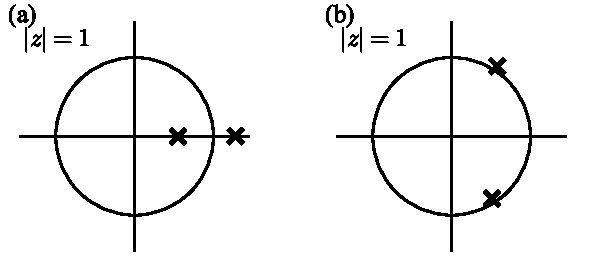
\includegraphics[width=0.72\textwidth]{fig_4.16.pdf}
\caption*{图 4.16\quad $\dfrac{1}{(z-\alpha-\mathrm{i}0^{+})^{2}+1-(\alpha+\mathrm{i}0^{+})^{2}}$ 的两个极点：(a) $|\alpha|>1$ 情形；(b) $|\alpha|<1$ 情形。若不存在 $\mathrm{i}0^{+}$ 项，$|\alpha|<1$ 的两个极点将位于单位圆 $|z|=1$ 上。}
\end{figure}

\subsection{注记：一些计算细节}

\subsubsection{二维中 $\pi^{\perp}$ 的计算}

我们如下计算 $\pi^{22}$：
\begin{align*}
\pi^{22}(k\hat{\pmb{x}},\omega)
&= \frac{1}{4m^{2}}\, \frac{1}{4\pi^{2}} \int \mathrm{d}\Big(\frac{q^{2}}{2m}\Big) \mathrm{d}\theta\;
\delta(\epsilon(\pmb{q}) - \mu)\, \frac{\pmb{k}\cdot\pmb{q}}{\omega - \frac{\pmb{k}\cdot\pmb{q}}{m} + \mathrm{i}0^{+}}\; (2q_{2} + k_{2})^{2}\\
&= \frac{1}{m^{2}}\, \frac{1}{4\pi^{2}} \int \mathrm{d}\theta\;
\frac{k k_{F} \cos(\theta)\, k_{F}^{2} \sin^{2}(\theta)}{\omega - \frac{k k_{F}\cos(\theta)}{m} + \mathrm{i}0^{+}}
= \frac{k_{F}^{2}}{4\pi^{2} m} \int \mathrm{d}\theta\;
\frac{\cos(\theta) \sin^{2}(\theta)}{\frac{\omega}{v_{F} k} - \cos(\theta) + \mathrm{i}0^{+}}
\end{align*}
以及（见图 4.16）
\begin{align*}
\int \mathrm{d}\theta\; \frac{\cos(\theta) \sin^{2}(\theta)}{\alpha + \mathrm{i}0^{+} - \cos(\theta)}
&= \frac{1}{4} \oint_{|z|=1} \mathrm{d}z\; \frac{1}{\mathrm{i} z^{3}}\, \frac{(z^{2}-1)^{2}(z^{2}+1)}{(z-\alpha)^{2} + 1 - \alpha^{2}}\\
&= \left\{
\begin{array}{ll}
-\pi + 2\pi\alpha^{2} - 2\pi \mathrm{i} \alpha \sqrt{1-\alpha^{2}} & \text{对于 } |\alpha| < 1\\
-\pi + 2\pi\alpha^{2} - 2\pi |\alpha| \sqrt{\alpha^{2}-1} & \text{对于 } |\alpha| > 1
\end{array} \right.
\end{align*}

\subsubsection{三维中 $\pi^{\perp}$ 的计算}

为计算 $\pi^{\perp}$，我们可取 $\pmb{k} = (0, 0, k)$ 并利用
\begin{align*}
\pi^{\perp}(\omega, k) &= \pi^{11}(k\hat{\pmb{z}}, \omega)
= \frac{1}{4m^{2}}\, \frac{1}{8\pi^{3}} \int q\, \mathrm{d}\Big(\frac{q^{2}}{2m}\Big) \mathrm{d}\phi\, \mathrm{d}\theta\;
\frac{\cos(\theta)\, \delta(\epsilon(\pmb{q}))\, \pmb{k}\cdot\pmb{q}}{\omega - \frac{\pmb{k}\cdot\pmb{q}}{m} + \mathrm{i}0^{+}}\; (2q_{1} + k_{1})^{2}\\
&= \frac{1}{m^{2}}\, \frac{1}{8\pi^{3}} \int \mathrm{d}\phi\, \mathrm{d}\theta\;
\frac{k \cos(\theta)\, k_{F}^{4} \sin^{3}(\theta) \cos^{2}(\phi)}{\omega - \frac{k k_{F}\cos(\theta)}{m} + \mathrm{i}0^{+}}
= \frac{k_{F}^{3}}{8\pi^{2} m} \int_{-1}^{1} \mathrm{d}t\; \frac{t(1-t^{2})}{\frac{\omega}{v_{F} k} - t + \mathrm{i}0^{+}}\\
&= \frac{k_{F}^{3}}{8\pi^{2} m} \left( -\frac{4}{3} + 2\frac{\omega^{2}}{v_{F}^{2} k^{2}}
- \frac{\omega}{v_{F} k} \Big( 1 - \frac{\omega^{2}}{v_{F}^{2} k^{2}} \Big)
\Big( \ln \frac{|\omega - v_{F} k|}{|\omega + v_{F} k|} + \mathrm{i}\pi \Theta(v_{F} k - |\omega|) \Big) \right)
\end{align*}
我们还注意到 $\rho = k_{F}^{3}/6\pi^{2}$。

\section{绝缘体的线性响应与量子化霍尔电导}

\begin{keypoints}
\item 绝缘体的霍尔电导是一个拓扑量，并且是量子化的。
\end{keypoints}

在上一节中，我们讨论了具有费米面的自由费米子系统的线性响应。这些响应是由跨费米面的粒子--空穴激发引起的。在本节中，我们想讨论绝缘体的线性响应。这里，``绝缘体''指的是任何具有有限能隙的态。（这样的态也称为刚性态（rigid state）。）由于没有低能激发，响应的虚部在小 $\omega$ 处为零（即不存在低能耗散）。

考虑一个与电磁场耦合的相互作用费米子系统：$\mathcal{L}(c, c^{\dagger}, A_{\mu}) + \mathcal{L}_{\mathrm{gauge}}(A_{\mu})$。我们将要得到的结果非常普遍，甚至不需要知道 $\mathcal{L}(c, c^{\dagger}, A_{\mu})$ 的具体形式。我们只假设费米子的基态具有有限能隙，并且 $\mathcal{L}(c, c^{\dagger}, A_{\mu})$ 在规范变换
\begin{equation*}
c(x^{\mu}) \to \mathrm{e}^{\mathrm{i}\phi(x^{\mu})} c(x^{\mu}), \qquad A_{\mu} \to A_{\mu} + \partial_{\mu} \phi(x^{\mu}).
\end{equation*}
下不变。把费米子积掉之后，我们得到规范场的一个有效作用量：
\begin{align*}
&\mathcal{L}_{\mathrm{eff}}(A_{\mu}) = \mathcal{L}_{\mathrm{gauge}}(A_{\mu}) + \delta\mathcal{L}_{\mathrm{eff}}(A_{\mu})\\
&\delta\mathcal{L}_{\mathrm{eff}}(A_{\mu}) = -\frac{1}{2} \int \mathrm{d}x\, \mathrm{d}x'\; A_{\mu}(x) P^{\mu\nu}(x - x') A_{\nu}(x')
\end{align*}
其中 $\delta\mathcal{L}_{\mathrm{eff}}(A_{\mu})$ 是费米子的贡献，$P^{\mu\nu}(x-x')$ 是流--流关联函数。

对于绝缘体（或刚性态），$\delta\mathcal{L}_{\mathrm{eff}}$ 是局域的，而且 $P^{\mu\nu}_{k_{\mu}}$ 在频率--动量空间中是 $k_{\mu}$ 的多项式。这与上一节为金属算出的 $P^{\mu\nu}_{k_{\mu}}$ 形成鲜明对比。金属在小 $(\pmb{k}, \omega)$ 极限下的奇异性是由跨费米面的无能隙粒子--空穴激发引起的。

这里 $\delta\mathcal{L}_{\mathrm{eff}}(A_{\mu})$ 也应当是规范不变的。因此，$\delta\mathcal{L}_{\mathrm{eff}}(A_{\mu})$ 应当只通过场强 $\pmb{E}$ 和 $\pmb{B}$ 依赖于 $A_{\mu}$。于是 $\delta\mathcal{L}_{\mathrm{eff}}$ 具有如下形式：
\begin{equation*}
\delta\mathcal{L}_{\mathrm{eff}} = -\frac{1}{2} \big( B_{i} \chi^{ij} B_{j} + E_{i} p^{ij} E_{j} \big) + \dots
\end{equation*}
其中``$\dots$''代表更高阶导数项。张量 $\chi^{ij}$ 是磁化率，$p^{ij}$ 代表介电常数的一个修正。一般而言，以上就是绝缘体线性响应仅有的几种形式。

然而，在 $2+1$ 维中，$\delta\mathcal{L}_{\mathrm{eff}}$ 还可以包含一个新项——Chern--Simons 项——如下：
\begin{equation*}
\delta\mathcal{L}_{\mathrm{eff}} = \frac{K}{4\pi} A_{\mu} \partial_{\nu} A_{\lambda} \epsilon^{\mu\nu\lambda} - \frac{1}{2} \big( B_{i} \chi^{ij} B_{j} + E_{i} p^{ij} E_{j} \big) + \dots
\end{equation*}
其中 $\mu, \nu, \lambda = 0, 1, 2$，而 $\epsilon^{\mu\nu\lambda}$ 是全反对称张量。尽管 Chern--Simons 项无法用场强写出，它却仍然是规范不变的。在规范变换
\begin{equation*}
A_{\mu} \to A_{\mu} + \partial_{\mu} f
\end{equation*}
下，作用量发生如下变化：
\begin{equation*}
S = \int_{V} \mathrm{d}x\; \mathcal{L}_{\mathrm{eff}} \to S + \oint_{S} \mathrm{d}S_{\mu}\, f\, \frac{K}{4\pi} \partial_{\nu} A_{\lambda} \epsilon^{\mu\nu\lambda}
\end{equation*}
其中 $V$ 是时空体积，$S$ 是 $V$ 的表面。我们看到，如果我们的系统生活在无边界的闭合时空上，那么 Chern--Simons 项就是规范不变的。

Chern--Simons 项的线性响应为
\begin{equation*}
J^{i} = -\frac{\delta S}{\delta A_{i}} = \frac{K}{2\pi} \partial_{0} A_{i} \epsilon^{ij} = \frac{K}{2\pi} E_{i} \epsilon^{ij}
\end{equation*}
我们看到 Chern--Simons 项给出霍尔电导 $\sigma_{xy} = K/2\pi$（如果把 $e$ 和 $\hbar$ 放回去，则 $\sigma_{xy} = Ke^{2}/h$）。

下面我们将证明霍尔电导 $\sigma_{xy}$ 或 $K$ 是量子化的（Thouless et al., 1982; Avron et al., 1983）。首先，让我们考虑一个周期系统和一个特殊的规范场位形：
\begin{equation*}
A_{1} = \frac{\theta_{1}(t)}{L_{1}}, \qquad A_{2} = \frac{\theta_{2}(t)}{L_{2}}, \qquad A_{0} = 0 \tag{4.4.1}
\end{equation*}
其中 $L_{1,2}$ 是系统在 $x$ 与 $y$ 方向上的尺寸。费米子的多体基态 $|\pmb{\theta}\rangle$ 由 $\pmb{\theta} = (\theta_{1}, \theta_{2})$ 参量化。如果我们把费米子积掉，就会得到一个有效拉格朗日量 $\delta L_{\mathrm{eff}} = \int \mathrm{d}^{2}\pmb{x}\; \delta\mathcal{L}_{\mathrm{eff}}$：
\begin{equation*}
\delta L_{\mathrm{eff}} = \frac{K}{4\pi} \theta_{i} \dot{\theta}_{j} \epsilon^{ij} + \dot{\theta}_{i} p^{ij} \dot{\theta}_{j}
\end{equation*}
其中第一项来自 Chern--Simons 项，第二项来自 $\pmb{E}^{2}$ 项。如果我们把 $\pmb{\theta}$ 看作一个粒子的坐标，那么 $\delta S$ 描写的就是一个处于均匀``磁场'' $b$ 中的二维带电粒子：
\begin{align*}
\delta L_{\mathrm{eff}} &= a_{i}(\pmb{\theta}) \dot{\theta}_{i} + \dot{\theta}_{i} p^{ij} \dot{\theta}_{j}\\
a_{1} &= -\frac{K}{4\pi} \theta_{2}, \qquad a_{2} = \frac{K}{4\pi} \theta_{1}, \qquad b = \partial_{\theta_{1}} a_{2} - \partial_{\theta_{2}} a_{1} = \frac{K}{2\pi}
\end{align*}

在 4.4.1 节中，我们将证明费米子态 $|\theta_{1}, \theta_{2}\rangle$、$|\theta_{1} + 2\pi, \theta_{2}\rangle$ 与 $|\theta_{1}, \theta_{2} + 2\pi\rangle$ 由规范变换联系在一起。物理上，这意味着 $|\theta_{1}, \theta_{2}\rangle$、$|\theta_{1} + 2\pi, \theta_{2}\rangle$ 与 $|\theta_{1}, \theta_{2} + 2\pi\rangle$ 其实是同一个物理态（见 6.1 节的讨论）。因此，$\delta L_{\mathrm{eff}}$ 实际上描写的是一个环面上的粒子，环面由 $0 < \theta_{1} < 2\pi$ 与 $0 < \theta_{2} < 2\pi$ 参量化。

让我们让粒子沿回路 $C$：$(0,0) \to (2\pi,0) \to (2\pi,2\pi) \to (0,2\pi) \to (0,0)$ 移动。这样一圈移动所积累的相位由 $C$ 所包围的``磁''通量给出：
\begin{equation*}
\oint_{C} \mathrm{d}\pmb{\theta} \cdot \pmb{a} = \int_{D} \mathrm{d}^{2}\pmb{\theta}\; b = 2\pi K
\end{equation*}
其中 $D$ 是回路 $C$ 所围的面积。在任何闭合曲面（例如球面或环面）上，任何回路都会围住该回路两侧的两个曲面（见图 6.5）。这里的 $D$ 只是 $C$ 所围两个曲面中的一个。$C$ 所围的另一个曲面 $D'$ 面积为零（因为 $D$ 覆盖了环面的全部面积）。所以相位 $\oint_{C} \mathrm{d}\pmb{\theta} \cdot \pmb{a}$ 也可以写成 $\int_{D'} \mathrm{d}^{2}\pmb{\theta}\; b = 0$。为保持一致，$\int_{D} \mathrm{d}^{2}\pmb{\theta}\; b$ 与 $\int_{D'} \mathrm{d}^{2}\pmb{\theta}\; b$ 应当代表同一个相位。于是
\begin{equation*}
\int_{D} \mathrm{d}^{2}\pmb{\theta}\; b = 2\pi \times \text{整数}
\end{equation*}

从数学上可以证明，穿过任何闭合曲面的总磁通量必须量子化为整数。这正是磁单极子的磁荷量子化的原因。对我们的情形，这意味着 $K$ 量子化为整数（另见 4.4.1 节）。

我们想强调，$K$ 的量子化是非常普遍的。它适用于费米子和/或玻色子的任何相互作用系统。唯一的假设是基态 $|\pmb{\theta}\rangle$ 不简并。于是，\emph{如果环面上的多体基态不简并且具有有限能隙，那么系统的霍尔电导就量子化为整数 $\times\ e^{2}/h$}。我们想指出，如果多体基态具有简并（见 8.2.1 节），那么 $K$ 和霍尔电导就可以是一个\emph{有理}数（Niu et al., 1985）。

霍尔电导的量子化有一些有趣的推论。让我们考虑均匀磁场中的一个无相互作用电子系统。如果 $n$ 个朗道能级被填满，系统就会有有限能隙，且霍尔电导为 $ne^{2}/h$（即 $K = n$）。现在让我们加入相互作用、周期势，甚至无规势。只要能隙在此过程中始终不闭合，霍尔电导就不能改变！由于霍尔电导对任何微扰都是稳健的，我们称它为一个\emph{拓扑}量子数。改变霍尔电导的唯一办法是使能隙闭合，这将诱导一个量子相变。

为了显式计算 $K$，我们注意到 $\int \mathrm{d}t\; \delta L_{\mathrm{eff}}$ 正是绝热演化 $|\pmb{\theta}(t)\rangle$ 的作用量。于是我们有 $\int \mathrm{d}t\; \delta L_{\mathrm{eff}} = \int \mathrm{d}t\; \mathrm{i}\langle \pmb{\theta}(t) | \frac{\mathrm{d}}{\mathrm{d}t} | \pmb{\theta}(t) \rangle$，或者（见式 (2.3.4)）
\begin{equation*}
\frac{K}{4\pi} \theta_{i} \dot{\theta}_{j} \epsilon^{ij} = \mathrm{i} \Big\langle \pmb{\theta}(t) \Big| \frac{\mathrm{d}}{\mathrm{d}t} \Big| \pmb{\theta}(t) \Big\rangle \tag{4.4.2}
\end{equation*}

这里我们想说明，作为费米子的基态，$|\pmb{\theta}(t)\rangle$ 的相位是不固定的。如果我们重新定义 $|\pmb{\theta}\rangle$ 的相位：$|\pmb{\theta}\rangle \to \mathrm{e}^{\mathrm{i}\varphi(\pmb{\theta})} |\pmb{\theta}\rangle$，那么贝里相项将改变一个全导数项：
\begin{equation*}
\Big\langle \pmb{\theta}(t) \Big| \frac{\mathrm{d}}{\mathrm{d}t} \Big| \pmb{\theta}(t) \Big\rangle \to \Big\langle \pmb{\theta}(t) \Big| \frac{\mathrm{d}}{\mathrm{d}t} \Big| \pmb{\theta}(t) \Big\rangle + \mathrm{i}\, \frac{\mathrm{d}\varphi}{\mathrm{d}t}
\end{equation*}
因此，Chern--Simons 项与贝里相之间的关系式 (4.4.2) 不可能是正确的，因为开放路径的贝里相甚至没有良定义（见 2.3 节）。正确的关系应当是式 (4.4.2) 沿一条闭合回路的积分：
\begin{equation*}
\oint \mathrm{d}t\; \frac{K}{4\pi} \theta_{i} \dot{\theta}_{j} \epsilon^{ij} = \mathrm{i} \oint \mathrm{d}t\; \Big\langle \pmb{\theta}(t) \Big| \frac{\mathrm{d}}{\mathrm{d}t} \Big| \pmb{\theta}(t) \Big\rangle
\end{equation*}
特别地，沿回路 $C$，贝里相由下式给出：
\begin{equation*}
2\pi K = \frac{\sigma_{xy} \hbar}{e^{2}} = \oint_{C} \mathrm{d}\pmb{\theta} \cdot \langle \pmb{\theta} | \mathrm{i} \partial_{\pmb{\theta}} | \pmb{\theta} \rangle \tag{4.4.3}
\end{equation*}

让我们用贝里相 (4.4.3) 来计算一个能带绝缘体的量子化霍尔电导，对此系统有
\begin{equation*}
H = \sum_{ij} c_{i}^{\dagger} t_{ij} c_{j} = \sum_{\pmb{k}} c_{\pmb{k}}^{\dagger} M(\pmb{k}) c_{\pmb{k}} \tag{4.4.4}
\end{equation*}
其中 $c_{i}$ 有 $n$ 个分量，$t_{ij}$ 是只依赖 $i - j$ 的 $n \times n$ 矩阵，$M(\pmb{k})$ 是 $t_{ij}$ 的傅里叶变换。与具有式 (4.4.1) 所给形式的均匀规范势 $\pmb{A}$ 耦合后，我们得到
\begin{equation*}
H = \sum_{ij} c_{i}^{\dagger} t_{ij}\, \mathrm{e}^{\mathrm{i}\pmb{A}\cdot(\pmb{i}-\pmb{j})} c_{j} = \sum_{\pmb{k}} c_{\pmb{k}}^{\dagger} M^{\theta}(\pmb{k}) c_{\pmb{k}}
\end{equation*}
然后设 $\psi^{\theta}_{a,\pmb{k}}$ 为 $M^{\theta}(\pmb{k})$ 的本征矢。这里 $\psi^{\theta}_{a,\pmb{k}}$ 由晶体动量 $\pmb{k}$ 标记，而 $a = 1, \dots, n$，其中 $a$ 标记第 $a$ 个本征矢。注意 $\psi^{\theta}_{a,\pmb{k}}$ 是一个 $n$ 维复矢量。

让我们假设基态 $|\pmb{\theta}\rangle$ 由填充 $a = 1$ 能带得到。我们有
\begin{equation*}
| \pmb{\theta} \rangle = \otimes_{\pmb{k}} \big| \psi^{\theta}_{1,\pmb{k}} \big\rangle
\end{equation*}
利用贝里相的可加关系，即
\begin{equation*}
\oint_{C} \mathrm{d}\pmb{\theta} \cdot \langle \pmb{\theta}, 0 | \mathrm{i} \partial_{\pmb{\theta}} | \pmb{\theta}, 0 \rangle
= \oint_{C} \mathrm{d}\pmb{\theta} \cdot \langle \pmb{\theta}, 1 | \mathrm{i} \partial_{\pmb{\theta}} | \pmb{\theta}, 1 \rangle
+ \oint_{C} \mathrm{d}\pmb{\theta} \cdot \langle \pmb{\theta}, 2 | \mathrm{i} \partial_{\pmb{\theta}} | \pmb{\theta}, 2 \rangle
\end{equation*}
若 $|\pmb{\theta}, 0\rangle = |\pmb{\theta}, 1\rangle \otimes |\pmb{\theta}, 2\rangle$，我们发现
\begin{equation*}
\oint_{C} \mathrm{d}\pmb{\theta} \cdot \langle \pmb{\theta} | \mathrm{i} \partial_{\pmb{\theta}} | \pmb{\theta} \rangle
= \sum_{\pmb{k}} \oint_{C} \mathrm{d}\pmb{\theta} \cdot (\psi^{\theta}_{1,\pmb{k}})^{\dagger} \mathrm{i} \partial_{\pmb{\theta}} \psi^{\theta}_{1,\pmb{k}} \tag{4.4.5}
\end{equation*}

\begin{figure}[H]
\centering
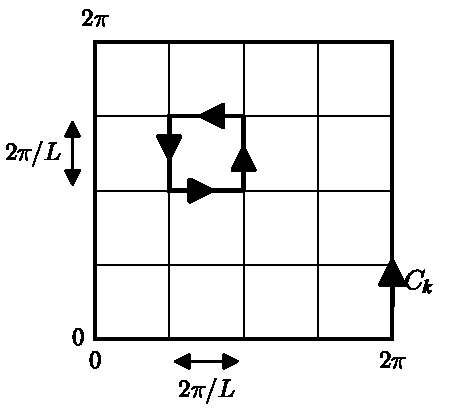
\includegraphics[width=0.72\textwidth]{fig_4.17.pdf}
\caption*{图 4.17\quad 固定的 $\pmb{k}$ 下由 $\pmb{k}' = \pmb{k} + \pmb{\theta} L^{-1}$ 扫出的小回路。所有不同 $\pmb{k}$ 的小回路覆盖整个布里渊区。沿所有小回路的回路积分对应于沿回路 $C_{\pmb{k}}$ 的回路积分，因为来自内部连线的贡献相互抵消。}
\end{figure}

我们如何计算 $\psi^{\theta}_{1,\pmb{k}}$ 的贝里相？这里我们注意到 $M^{\theta}(\pmb{k}) = M(\pmb{k} + \pmb{\theta} L^{-1})$，其中为简单起见我们已在式 (4.4.1) 中取了 $L_{1} = L_{2} = L$。于是，$\psi^{\theta}_{1,\pmb{k}}$ 是 $M(\pmb{k} + \pmb{\theta} L^{-1})$ 的本征矢。设 $\psi_{a,\pmb{k}'}$ 为 $M(\pmb{k}')$ 的本征矢；那么当 $\pmb{k}' = \pmb{k} + \pmb{\theta} L^{-1}$ 时，$\psi^{\theta}_{1,\pmb{k}} = \psi_{1,\pmb{k}'}$。当 $\pmb{\theta}$ 沿回路 $C$ 移动时，对固定的 $\pmb{k}$，$\pmb{k}'$ 沿一个小回路移动（见图 4.17）。由于分立的 $\pmb{k}$ 具有 $(n_{1} \frac{2\pi}{L}, n_{2} \frac{2\pi}{L})$ 的形式，我们看到不同 $\pmb{k}$ 的所有小回路互不重叠地覆盖了整个布里渊区。因此，式 (4.4.5) 中各 $\psi^{\theta}_{1,\pmb{k}}$ 的贝里相之和等于 $\psi_{1,\pmb{k}'}$ 沿一条包围整个布里渊区的大回路 $C_{\pmb{k}}$ 的贝里相：
\begin{align*}
2\pi K &= \oint_{C_{\pmb{k}}} \mathrm{d}\pmb{k} \cdot \psi_{1,\pmb{k}}^{\dagger}\, \mathrm{i} \partial_{\pmb{k}} \psi_{1,\pmb{k}}\\
&= \int \mathrm{d}^{2}\pmb{k}\; \mathrm{i} \big[ (\partial_{k_{x}} \psi_{1,\pmb{k}}^{\dagger}) (\partial_{k_{y}} \psi_{1,\pmb{k}}) - (\partial_{k_{y}} \psi_{1,\pmb{k}}^{\dagger}) (\partial_{k_{x}} \psi_{1,\pmb{k}}) \big] \tag{4.4.6}
\end{align*}
如果填充了几个能带，那么我们需要对每个能带的贡献求和。

作为一个具体例子，考虑正方格子上如下的依赖自旋的跃迁哈密顿量：
\begin{equation*}
H = \sum_{i} c_{i}^{\dagger} t_{ij} c_{j}
\end{equation*}
其中 $2 \times 2$ 的跃迁矩阵为
\begin{equation*}
t_{\pmb{i}, \pmb{i}+\pmb{x}} = t \sigma^{x}, \qquad t_{\pmb{i}, \pmb{i}+\pmb{y}} = t \sigma^{y}, \qquad t_{\pmb{i}, \pmb{i}+\pmb{x}+\pmb{y}} = t' \sigma^{z},
\end{equation*}

\begin{figure}[H]
\centering
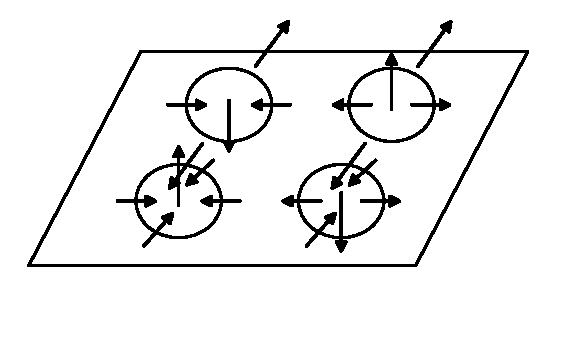
\includegraphics[width=0.72\textwidth]{fig_4.18.pdf}
\caption*{图 4.18\quad 箭头表示 $\pmb{B}$ 的方向。缠绕数仅收到来自四个点 $\pmb{k} = (\pm\pi/2, \pm\pi/2)$ 附近的贡献。在每个点附近，$\pmb{B}$ 覆盖半球，贡献缠绕数 $1/2$。总缠绕数为 2。}
\end{figure}

在动量空间中，哈密顿量变为
\begin{equation*}
H_{\pmb{k}} = 2 t \cos(k_{x}) \sigma^{x} + 2 t \cos(k_{x}) \sigma^{y} + 2 t' \cos(k_{x} + k_{y}) \sigma^{z} = -\pmb{B}(\pmb{k}) \cdot \sigma
\end{equation*}
（译注：按物理内容与图 4.18，$\sigma^{y}$ 项的系数应为 $\cos(k_{y})$；原书该项也印作 $\cos(k_{x})$。）

我们看到系统有两个能带。这里的 $H_{\pmb{k}}$ 就像磁场 $\pmb{B}(\pmb{k})$ 中一个自旋 $1/2$ 的自旋的哈密顿量。较低的能带对应于沿 $\pmb{B}$ 方向的自旋。当沿 $\pmb{k}$ 空间中的一条回路移动时，沿 $\pmb{B}(\pmb{k})$ 方向的自旋在自旋空间的单位球上扫出一条闭合回路，并产生一个贝里相。如果填充较低的能带，那么只要选取包围整个布里渊区的回路，霍尔电导就可以由上述自旋 $1/2$ 的贝里相算出。从小 $t'$ 极限下 $\pmb{B}(\pmb{k})$ 的表达式我们看到，除四个点 $\pmb{k} = (\pm\pi/2, \pm\pi/2)$ 附近外，$\pmb{B}$ 都在 $x$--$y$ 平面内。考察 $\pmb{k} = (\pm\pi/2, \pm\pi/2)$ 附近的自旋（见图 4.18），我们发现，当 $\pmb{k}$ 扫过布里渊区时，$\pmb{B}/|\pmb{B}|$ 扫过单位球两次。或者更精确地说，$\pmb{B}(\pmb{k})/|\pmb{B}(\pmb{k})|$ 以缠绕数 2 把布里渊区 $S^{1} \times S^{1}$ 映射到单位球 $S^{2}$ 上。总贝里相因此为 $2 \times 2\pi$。我们求得 $K = 2$，半填充的跃迁系统的霍尔电导为 $\sigma_{xy} = 2e^{2}/h$。

\subsection*{问题 4.4.1}

对于哈密顿量 (4.4.4)，如果 $a = 1$ 能带被部分填充，试证明霍尔电导由对被填充能级的积分给出：
\begin{equation*}
\sigma_{xy} = \frac{e^{2}}{h}\, \frac{1}{2\pi} \int_{\text{filled}} \mathrm{d}^{2}\pmb{k}\; \mathrm{i} \big[ (\partial_{k_{x}} \psi_{1,\pmb{k}}^{\dagger}) (\partial_{k_{y}} \psi_{1,\pmb{k}}) - (\partial_{k_{y}} \psi_{1,\pmb{k}}^{\dagger}) (\partial_{k_{x}} \psi_{1,\pmb{k}}) \big]
\end{equation*}
在有限温度下，我们有
\begin{equation*}
\sigma_{xy} = \frac{e^{2}}{h}\, \frac{1}{2\pi} \int \mathrm{d}^{2}\pmb{k}\; n_{F}(\epsilon_{\pmb{k}})\, \mathrm{i} \big[ (\partial_{k_{x}} \psi_{1,\pmb{k}}^{\dagger}) (\partial_{k_{y}} \psi_{1,\pmb{k}}) - (\partial_{k_{y}} \psi_{1,\pmb{k}}^{\dagger}) (\partial_{k_{x}} \psi_{1,\pmb{k}}) \big]
\end{equation*}
（注意，对于部分填充的能带，$K$ 不量子化，因为 $|\pmb{\theta}\rangle$ 不具有 $2\pi$ 周期性，见式 (4.4.9)。）

\subsection{注记：$|\pmb{\theta}\rangle$ 的周期结构与 $K$ 的量子化}

首先，让我们研究费米子基态 $|\pmb{\theta}\rangle$ 在 $\pmb{\theta}$ 空间中的周期结构。这里 $|\pmb{\theta}\rangle$ 是如下哈密顿量的基态
\begin{equation*}
H_{\pmb{\theta}} = \int \mathrm{d}^{2}\pmb{x} \left( -\frac{\hbar^{2}}{2m} \sum_{j=1,2} c^{\dagger} \Big( \partial_{j} - \mathrm{i} A_{j} - \frac{\mathrm{i} \theta_{j}}{L_{j}} \Big)^{2} c + V(c^{\dagger} c) \right)
\end{equation*}
我们注意到 $U(1)$ 规范变换
\begin{align*}
c(\pmb{x}) &\to \mathrm{e}^{2\mathrm{i}\pi x_{1} L_{1}^{-1}} c(\pmb{x})\\
(A_{1}, A_{2}) &\to \Big( A_{1} + \frac{2\pi}{L_{1}},\, A_{2} \Big)
\end{align*}
和
\begin{align*}
c(\pmb{x}) &\to \mathrm{e}^{2\mathrm{i}\pi x_{2} L_{2}^{-1}} c(\pmb{x})\\
(A_{1}, A_{2}) &\to \Big( A_{1},\, A_{2} + \frac{2\pi}{L_{2}} \Big)
\end{align*}
并不改变费米子算符 $c(\pmb{x})$ 在 $x$ 与 $y$ 方向上的周期性边界条件。然而，这些规范变换生成如下平移：$(\theta_{1}, \theta_{2}) \to (\theta_{1} + 2\pi, \theta_{2})$ 与 $(\theta_{1}, \theta_{2}) \to (\theta_{1}, \theta_{2} + 2\pi)$。或者更精确地说，我们有
\begin{align*}
H_{\theta_{1}+2\pi, \theta_{2}} &= W_{1} H_{\theta_{1}, \theta_{2}} W_{1}^{\dagger}
& W_{1} &= \mathrm{e}^{\mathrm{i} \int \mathrm{d}^{2}\pmb{x}\; 2\pi x_{1} L_{1}^{-1} c^{\dagger} c}\\
H_{\theta_{1}, \theta_{2}+2\pi} &= W_{2} H_{\theta_{1}, \theta_{2}} W_{2}^{\dagger}
& W_{2} &= \mathrm{e}^{\mathrm{i} \int \mathrm{d}^{2}\pmb{x}\; 2\pi x_{2} L_{2}^{-1} c^{\dagger} c}
\end{align*}
因此，如果 $|\pmb{\theta}\rangle$ 是 $\pmb{\theta}$ 处的多体基态，那么 $W_{1}|\pmb{\theta}\rangle$ 就是平移后的 $\pmb{\theta}$ 处的基态。于是
\begin{equation*}
\big| \theta_{1} + 2\pi, \theta_{2} \big\rangle = \mathrm{e}^{\mathrm{i} f_{1}(\pmb{\theta})} W_{1} \big| \theta_{1}, \theta_{2} \big\rangle \tag{4.4.7}
\end{equation*}
其中 $f_{1}(\pmb{\theta})$ 可任选。类似地，我们有
\begin{equation*}
\big| \theta_{1}, \theta_{2} + 2\pi \big\rangle = \mathrm{e}^{\mathrm{i} f_{2}(\pmb{\theta})} W_{2} \big| \theta_{1}, \theta_{2} \big\rangle \tag{4.4.8}
\end{equation*}

这两个幺正算符 $\mathrm{e}^{\mathrm{i} f_{1}(\pmb{\theta})} W_{1}$ 与 $\mathrm{e}^{\mathrm{i} f_{2}(\pmb{\theta})} W_{2}$ 生成把 $|\theta_{1}, \theta_{2}\rangle$、$|\theta_{1} + 2\pi, \theta_{2}\rangle$ 与 $|\theta_{1}, \theta_{2} + 2\pi\rangle$ 联系起来的那些规范变换。

我们总可以重新定义 $|\pmb{\theta}\rangle$ 的相位：$|\pmb{\theta}\rangle \to \mathrm{e}^{\mathrm{i} \phi(\pmb{\theta})} |\pmb{\theta}\rangle$，使得 $f_{1} = 0$，只要我们选择 $\phi$ 满足
\begin{equation*}
\phi(\theta_{1} + 2\pi, \theta_{2}) - \phi(\theta_{1}, \theta_{2}) = f_{1}(\theta_{1}, \theta_{2}).
\end{equation*}
那么，由
\begin{equation*}
\big| \theta_{1} + 2\pi, \theta_{2} + 2\pi \big\rangle = \mathrm{e}^{\mathrm{i} f_{2}(\theta_{1}+2\pi, \theta_{2})} W_{2} \big| \theta_{1} + 2\pi, \theta_{2} \big\rangle
\end{equation*}
我们得到
\begin{equation*}
W_{1} \big| \theta_{1}, \theta_{2} + 2\pi \big\rangle = \mathrm{e}^{\mathrm{i} f_{2}(\theta_{1}+2\pi, \theta_{2})} W_{2} W_{1} \big| \theta_{1}, \theta_{2} \big\rangle
\end{equation*}
由于 $[W_{1}, W_{2}] = 0$，我们有
\begin{equation*}
\big| \theta_{1}, \theta_{2} + 2\pi \big\rangle = \mathrm{e}^{\mathrm{i} f_{2}(\theta_{1}+2\pi, \theta_{2})} W_{2} \big| \theta_{1}, \theta_{2} \big\rangle
\end{equation*}
把上式与式 (4.4.8) 比较，我们发现
\begin{equation*}
\mathrm{e}^{\mathrm{i} f_{2}(\theta_{1}+2\pi, \theta_{2})} = \mathrm{e}^{\mathrm{i} f_{2}(\theta_{1}, \theta_{2})}
\end{equation*}
我们看到 $|\pmb{\theta}\rangle$ 在 $\theta_{1}$ 与 $\theta_{2}$ 上以 $2\pi$ 为周期准周期：
\begin{align*}
\big| \theta_{1} + 2\pi, \theta_{2} \big\rangle &= W_{1} \big| \theta_{1}, \theta_{2} \big\rangle\\
\big| \theta_{1}, \theta_{2} + 2\pi \big\rangle &= \mathrm{e}^{\mathrm{i} f_{2}(\theta_{1}, \theta_{2})} W_{2} \big| \theta_{1}, \theta_{2} \big\rangle \tag{4.4.9}
\end{align*}
其中 $W_{1,2}$ 是不依赖 $\pmb{\theta}$ 的幺正算符。

利用 $\langle \pmb{\theta} | \partial_{\pmb{\theta}} | \pmb{\theta} \rangle = \langle \pmb{\theta} | W_{1,2}^{\dagger} \partial_{\pmb{\theta}} W_{1,2} | \pmb{\theta} \rangle$ 与式 (4.4.9)，我们可以把贝里相 (4.4.3) 约化为
\begin{equation*}
2\pi K = \int \mathrm{d}\theta_{1}\; \partial_{\theta_{1}} f_{2}(\theta_{1}, 0) = f_{2}(2\pi, 0) - f_{2}(0, 0)
\end{equation*}
由于 $\mathrm{e}^{\mathrm{i} f_{2}(\theta_{1}, \theta_{2})}$ 在 $\theta_{1}$ 上是周期的，我们发现 $f_{2}(2\pi, 0) - f_{2}(0, 0) = 2\pi \times$ 整数，即 $K$ 量子化为一个整数。

 % 本文件由 scripts/assemble.py 自动装配，勿手改（改 parts/ 后重跑）
% 第5章 相互作用费米子系统

% 第5章 INTERACTING FERMION SYSTEMS
\chapter{相互作用费米子系统}

自然界中的电子系统具有相当强的库仑相互作用。材料的许多有趣性质——如磁性、超导电性等等——都源于相互作用。在本章中，我们将研究电子--电子相互作用的效应。特别地，我们将讨论金属的 Landau 费米液体理论以及由相互作用诱导的对称性破缺相变。

\section{正交性灾变与 X 射线谱}

\begin{keypoints}
\item 正交性灾变（orthogonality catastrophe）是展示多体效应如何影响费米子格林函数以及相关实验结果的一种现象。
\item 正交性灾变是一种普遍现象，可以出现在许多系统中，例如 X 射线谱、隧穿进入量子点的 $I$--$V$ 曲线等。
\end{keypoints}

\subsection{物理模型}

X 射线谱由金属中芯能级（core level）与导带（conduction band）之间的跃迁引起（见图 5.1(a)）。X 射线的吸收把一个电子从芯能级移出并把它放入一个未被占据的带态；发射则把一个电子从被占据的带态移到未被占据的芯态。系统可以用如下哈密顿量建模：
\begin{equation*}
H=\sum_{\pmb{k}}\epsilon_{\pmb{k}}c_{\pmb{k}}^{\dagger}c_{\pmb{k}}-E_CC^{\dagger}C+\Gamma(\mathrm{e}^{-\mathrm{i}\omega t}c(0)C^{\dagger}+\text{h.c.})\tag{5.1.1}
\end{equation*}
其中 $C$ 描述 $\pmb{x}=0$ 处的一个芯电子，$\Gamma\mathrm{e}^{-\mathrm{i}\omega t}$ 是 X 射线诱导的含时耦合。为简单起见，本节中我们假设电子无自旋。

\begin{figure}[H]
\centering
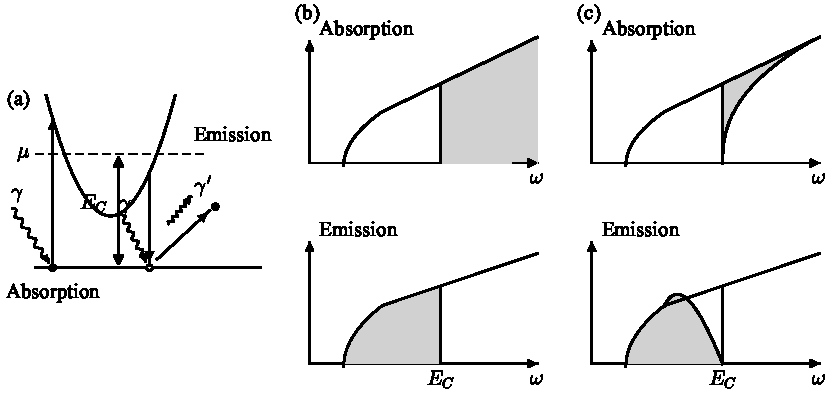
\includegraphics[width=0.72\textwidth]{fig_5.1.pdf}
\caption*{图 5.1\quad (a) X 射线吸收/发射由金属中芯能级与导带之间的跃迁引起。图中还画出了这些跃迁的 X 射线谱：(b) 无相互作用时；(c) 有相互作用时。}
\end{figure}

注意，发射率等于从导带流向芯态的电流。根据线性响应理论，发射率为
\begin{align*}
A_{em}(\omega) &= \langle 0|\mathrm{i}\Gamma(\mathrm{e}^{-\mathrm{i}\omega t}I(t)-\text{h.c.})|0\rangle\\
&= \Gamma^2\int^t\mathrm{d}t'\left(\mathrm{e}^{-\mathrm{i}\omega(t-t')}\langle 0|[I(t),I^{\dagger}(t')]|0\rangle+\text{h.c.}\right)
\end{align*}
其中 $I(t)=c(0,t)C^{\dagger}(t)$。我们可以用芯电子和传导电子的谱函数（见式 (4.2.17)）把发射率 $A_{em}$ 表示如下：
\begin{equation*}
A_{em}(\omega)=-2\pi\Gamma^2\int\mathrm{d}\nu\,\left(A_{c-}^{0}(\nu)A_{C+}^{0}(\nu-\omega)-A_{c+}^{0}(\nu)A_{C-}^{0}(\nu-\omega)\right)
\end{equation*}
对自由费米子，谱函数由态密度给出（如式 (4.2.18)）。如果我们把能量零点取在费米面上，则有
\begin{align*}
&A_{c-}^{0}(\omega)=n_F(\omega)N(\omega+E_F),\qquad A_{c+}^{0}(\omega)=(1-n_F(\omega))N(\omega+E_F)\\
&A_{C-}^{0}(\omega)=0,\qquad\qquad\qquad\qquad\quad\ \ A_{C+}^{0}(\omega)=\delta(\omega+E_C)
\end{align*}
我们注意到，在发射之前芯态是完全空的。这正是上述非平衡芯电子谱函数的来源。我们求得
\begin{equation*}
A_{em}(\omega)=2\pi\Gamma^2n_F(\omega-E_C)N(E_F-E_C+\omega)
\end{equation*}
发射率直接测量自由费米子的态密度（见图 5.1(b)；注意 $E_C>0$）。在零温下，$A_{em}(\omega)$ 在 $\omega=E_C$ 处有一个阶梯状的跳变，它标志着费米面的锐利性。如果我们采用相互作用电子的谱函数，上述结果也适用于相互作用的电子。

\begin{figure}[H]
\centering
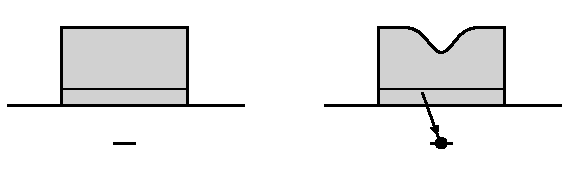
\includegraphics[width=0.72\textwidth]{fig_5.2.pdf}
\caption*{图 5.2\quad 如果芯电子与传导电子之间存在相互作用，那么隧穿之后传导电子的密度必须发生改变。}
\end{figure}

\subsection*{问题 5.1.1}

计算吸收率谱 $A_{obs}(\omega)$。（译注：原书符号排印如此，按上下文应为吸收率谱 $A_{abs}(\omega)$。）

\subsection{正交性灾变的物理}

\begin{keypoints}
\item 正交性灾变是由于描述形变费米海与未形变费米海的两个多体波函数之间的交叠消失而引起的。
\end{keypoints}

现在我们想在芯电子与传导电子之间引入相互作用。我们将看到，这样的相互作用会显著地改变发射/吸收率在 $\omega=E_C$ 处的边缘奇异性。

物理图像示于图 5.2。当芯电子与传导电子之间没有相互作用时，给定频率下发射的矩阵元涉及某个能量处传导电子的单粒子波函数与芯电子波函数之间的矩阵元。为了推广到相互作用情形，我们应当把上述矩阵元看作两个多体本征态之间的矩阵元：一个本征态具有填满的费米海（Fermi sea）和空的芯态，另一个本征态在费米海中有一个空穴且芯态被填满。当存在相互作用时，芯电子会改变传导电子的密度，从而改变多体电子波函数。于是，发射的矩阵元涉及以下两个本征态之间的矩阵元：一个具有填满但形变的费米海和空的芯态，另一个在均匀费米海中有一个空穴且芯态被填满。我们可以把上述矩阵元近似为单粒子态之间的矩阵元与均匀费米海和形变费米海这两个多体态之间交叠的乘积。如果交叠有限，那么上一小节的讨论在 $\omega$ 靠近 $E_C$ 处仍然成立，只是隧穿振幅 $\Gamma$ 可能被一个有限因子缩小。然而，如果交叠为零，那么上一小节的结果就必须作重大修改。特别地，$\omega=E_C$ 处的阶梯状奇异性会被破坏。这种现象称为红外灾变（infra-red catastrophe）或正交性灾变。

我们知道，自由费米子的多体波函数可以由单体波函数通过 Slater 行列式构造如下：
\begin{equation*}
\Psi(\pmb{x}_1,\ldots,\pmb{x}_N)=\mathrm{Det}[\psi_i(\pmb{x}_j)]
\end{equation*}
其中 $\psi_i(\pmb{x})$ 是单体波函数，$[\psi_i(\pmb{x}_j)]$ 是如下矩阵：
\begin{equation*}
[\psi_i(\pmb{x}_j)]\equiv
\begin{pmatrix}
\psi_1(\pmb{x}_1) & \psi_1(\pmb{x}_2) & \cdots\\
\psi_2(\pmb{x}_1) & \psi_2(\pmb{x}_2) & \cdots\\
\cdots & \cdots & \ddots
\end{pmatrix}
\end{equation*}
均匀费米海的多体波函数 $\Psi_0$ 由平面波 $\psi_i(\pmb{x})=\mathrm{e}^{\mathrm{i}\pmb{k}_i\cdot\pmb{x}}$ 构造，其中 $\pmb{k}_i$ 取遍所有能量低于费米能 $E_F$ 的动量。形变费米海的多体波函数 $\Psi$ 则由芯电子的势存在时的本征函数构造。于是我们可以计算交叠 $\langle\Psi_0|\Psi\rangle$，以判断是否存在正交性灾变。

为了在一个简单的计算中说明我们的论点，我们将把费米子当作由密度 $\rho(\pmb{x})$ 描述的流体来计算 $\langle\Psi_0|\Psi\rangle$。这种处理在一维给出正确的结果，但在高于一维时给出错误的结果。这种方法称为流体动力学方法（hydrodynamical approach），或费米子系统的玻色化（bosonization）。让我们先把流体动力学方法发展起来。

\subsection{流体动力学方法（玻色化）}

\begin{keypoints}
\item 金属中的集体密度涨落可以用一个玻色型场论来描述。
\item 在一维，玻色理论对跨越费米面的粒子--空穴激发给出了完整的描述。
\end{keypoints}

可压缩流体（compressible fluid）的势能为
\begin{equation*}
V=\int\mathrm{d}^d\pmb{x}\,\frac{1}{2\chi}\rho^2(\pmb{x})
\end{equation*}
其中 $\chi$ 是压缩率。这里我们假设 $\rho(\pmb{x})$ 是围绕基态均匀密度 $\rho_0$ 的涨落。动能为
\begin{equation*}
K=\int\mathrm{d}^d\pmb{x}\,\frac{m\pmb{v}^2(\pmb{x})}{2}\rho_0=\int\mathrm{d}^d\pmb{x}\,\frac{m\pmb{j}^2(\pmb{x})}{2\rho_0}
\end{equation*}

\begin{figure}[H]
\centering
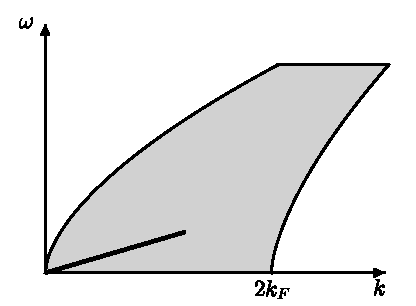
\includegraphics[width=0.72\textwidth]{fig_5.3.pdf}
\caption*{图 5.3\quad 线性模式的色散总是处于粒子--空穴连续谱之内。}
\end{figure}

其中 $\pmb{v}(\pmb{x})$ 是速度，$\pmb{j}(\pmb{x})=\pmb{v}(\pmb{x})\rho_0$ 是流体在 $\pmb{x}$ 处的流。于是，描述流体动力学的拉格朗日量为
\begin{equation*}
L=\int\mathrm{d}^d\pmb{x}\,\left[\frac{m\pmb{j}^2(\pmb{x})}{2\rho_0}-\frac{1}{2\chi}\rho^2(\pmb{x})\right]\tag{5.1.2}
\end{equation*}
由流守恒 $\partial_t\rho+\partial_{\pmb{x}}\cdot\pmb{j}=0$，我们得到 $\pmb{j}=-\frac{1}{\partial_{\pmb{x}}}\partial_t\rho$（假设 $\partial_{\pmb{x}}\times\pmb{j}=0$），于是拉格朗日量可以只用密度写出如下：
\begin{align*}
L &= \int\mathrm{d}^d\pmb{x}\,\left(\frac{m}{2\rho_0}\dot{\rho}\frac{1}{-\partial_{\pmb{x}}^2}\dot{\rho}-\frac{1}{2\chi}\rho^2\right)\tag{5.1.3}\\
&= \mathcal{V}^{-1}\sum_{\pmb{k}}\left(\frac{m}{2\rho_0}\dot{\rho}_{-\pmb{k}}\frac{1}{\pmb{k}^2}\dot{\rho}_{\pmb{k}}-\frac{1}{2\chi}\rho_{-\pmb{k}}\rho_{\pmb{k}}\right)\tag{5.1.4}
\end{align*}
其中 $\rho_{\pmb{k}}=\int\mathrm{d}^d\pmb{x}\,\rho(\pmb{x})\mathrm{e}^{-\mathrm{i}\pmb{k}\cdot\pmb{x}}$，$\mathcal{V}$ 是系统的体积。

这样的拉格朗日量与我们前面研究过的声子拉格朗日量 (3.3.15) 完全相同，其中 $A_{\pmb{k}}\allowbreak=m/\mathcal{V}\rho_0\pmb{k}^2$，$B_{\pmb{k}}\allowbreak=\frac{1}{\mathcal{V}\chi}$。声子由如下量子哈密顿量描述（见式 (3.3.18)）：
\begin{equation*}
H=\sum_{\pmb{k}\neq0}\Omega_{\pmb{k}}\alpha_{\pmb{k}}^{\dagger}\alpha_{\pmb{k}},\qquad
\Omega_{\pmb{k}}=\sqrt{\frac{B_{\pmb{k}}}{A_{\pmb{k}}}}=\sqrt{\frac{\rho_0}{m\chi}}\,|\pmb{k}|\tag{5.1.5}
\end{equation*}
对自由费米子，压缩率等于态密度：$\chi=N(E_F)$。我们求得流体动力学模式的速度为
\begin{align*}
v &= v_F && \text{当 } d=1\\
v &= \frac{1}{\sqrt{2}}v_F && \text{当 } d=2\\
v &= \frac{1}{\sqrt{3}}v_F && \text{当 } d=3
\end{align*}
流体动力学模式的色散总是处于粒子--空穴连续谱之内（见图 5.3）。可以证明，在 $d>1$ 维，单一线性模式的比热小于相应自由费米子系统的比热。因此，对 $d>1$，流体动力学处理并不能重现全部低能激发，它只描述某些平均的密度涨落。然而，在 $d=1$ 维和低温下，单个流体动力学模式的比热恰好等于相应自由费米子系统的比热，这暗示单个玻色模式重现了自由费米子系统的所有低能激发。这表明单个玻色模式在低能下是费米子系统的忠实描述，我们可以用玻色理论来描述费米子系统的低能性质。用玻色子描述一维费米子系统的方法称为玻色化（Tomonaga, 1950; Luttinger, 1963; Coleman, 1975）。

为了更细致地比较流体动力学模型与费米子模型，让我们考虑量子哈密顿量 (5.1.5) 中的多体低能激发。在一维，流体动力学哈密顿量 (5.1.5) 重现了相应费米子系统中所有低能激发的谱。为看清这一点，让我们把系统放在大小为 $L$ 的圆上，并假设基态能量为零。流体动力学模型有两个能量为 $E=2k_0v$、动量为 $K=2k_0$ 的本征态，即 $(\alpha_{k_0}^{\dagger})^2|0\rangle$ 和 $\alpha_{2k_0}^{\dagger}|0\rangle$，其中 $k_0=2\pi/L$。费米子系统在动量 $2k_0$ 处也有两个粒子--空穴激发态，它们具有完全相同的能量 $E=2k_0v_F=2k_0v$。这两个粒子--空穴态由 $c_{k_F+2k_0}^{\dagger}c_{k_F}|\psi_0\rangle$ 和 $c_{k_F+k_0}^{\dagger}c_{k_F-k_0}|\psi_0\rangle$ 给出。这里 $|\psi_0\rangle$ 是费米子系统的基态，其中单粒子态 $|k_F\rangle$、$|k_F-k_0\rangle$、……、$|-k_F\rangle$ 各被一个费米子占据。流体动力学模型有一个能量为 $E=2k_0v$、动量为 $K=0$ 的本征态，即 $\alpha_{-k_0}^{\dagger}\alpha_{k_0}^{\dagger}|0\rangle$。费米子系统也有一个具有相同动量和能量的粒子--空穴态，即 $c_{-k_F-k_0}^{\dagger}c_{-k_F}c_{k_F+k_0}^{\dagger}c_{k_F}|\psi_0\rangle$。事实上，流体动力学模型的激发谱与费米子模型的粒子--空穴激发谱完全相同（见问题 5.1.3）。流体动力学模型在低能和小动量下是费米子系统的忠实描述。

\subsection*{问题 5.1.2}

把 $\alpha_{\pmb{k}}$ 用 $\rho_{\pmb{k}}$ 和 $\dot{\rho}_{\pmb{k}}$ 表示。证明 $\alpha_{\pmb{k}}$ 携带确定的动量。

\subsection*{问题 5.1.3}

证明：在一维，流体动力学模型（固定粒子数）与费米子系统（固定费米子数）都具有以下性质。
\begin{enumerate}
\item[(a)] 有 $p_n$ 个能量为 $nk_0v_F$、动量为 $nk_0$ 的激发态，其中 $(p_0,p_1,p_2,\ldots)=(1,1,2,3,5,7,\ldots)$ 是分割数（partition numbers）。（如果找不到一般性的证明，可以验证到 $p_5$ 为止。）
\item[(b)] 有 $p_n$ 个能量为 $nk_0v_F$、动量为 $-nk_0$ 的激发态。
\item[(c)] 有 $p_{n-m}p_m$ 个能量为 $nk_0v_F$、动量为 $(n-2m)k_0$ 的态。因此，流体动力学模型与费米子系统在低能和小动量下具有完全相同的激发谱。
\end{enumerate}

\subsection*{问题 5.1.4}

\begin{enumerate}
\item[(a)] 由式 (4.3.2) 我们看到，压缩率 $\chi(\omega,\pmb{k})=-\Pi^{00}(\omega,\pmb{k})$ 含有虚部。使用这样的压缩率以及拉格朗日量 (5.1.2) 的运动方程，求出密度模式（声子）在 $d=1$、$d=2$、$d=3$ 维中的衰减率。把衰减率与模式的频率相比较。密度模式是否给出一个良好定义的声子？
\item[(b)] 事实上，(a) 小题并不太对。应当利用式 (5.1.2) 计算流体动力学模型的密度响应函数，然后通过让它拟合式 (4.3.2) 的费米子结果来得到 $\chi(\omega,\pmb{k})$。用这种方法求出 $\chi(\omega,\pmb{k})$。(a) 中的主要结果是否因新的 $\chi(\omega,\pmb{k})$ 而改变？
\end{enumerate}

\subsection{由流体动力学方法得到的正交性灾变}

\begin{keypoints}
\item 在流体动力学方法中，多体波函数的交叠可以由移位谐振子（shifted harmonic oscillators）容易地计算出来。
\end{keypoints}

当芯电子产生的势存在时，哈密顿量 (5.1.5) 含有一个附加项（见式 (3.3.17)）：
\begin{align*}
\delta H &= \int\mathrm{d}^d\pmb{x}\,\rho(\pmb{x})V(\pmb{x})=\mathcal{V}^{-1}\sum_{\pmb{k}}\rho_{\pmb{k}}V_{-\pmb{k}}=\mathcal{V}^{-1}\sum_{\pmb{k}}V_{-\pmb{k}}\frac{\alpha_{\pmb{k}}+\alpha_{\pmb{k}}^{\dagger}}{2u_{\pmb{k}}}\\
u_{\pmb{k}} &= \frac{1}{\sqrt{2}}(A_{\pmb{k}}B_{\pmb{k}})^{1/4}=\left(\frac{m}{4\mathcal{V}^2\rho_0\chi\pmb{k}^2}\right)^{1/4}
\end{align*}
这里 $H+\delta H$ 描述一组移位谐振子。势存在时系统的基态为
\begin{equation*}
|\Psi\rangle=\frac{\mathrm{e}^{-\mathcal{V}^{-1}\sum_{\pmb{k}}\frac{V_{-\pmb{k}}}{2\Omega_{\pmb{k}}u_{\pmb{k}}}\alpha_{\pmb{k}}^{\dagger}}|\Psi_0\rangle}
{\sqrt{\langle\Psi_0|\mathrm{e}^{-\mathcal{V}^{-1}\sum_{\pmb{k}}\frac{V^{*}_{-\pmb{k}}}{2\Omega_{\pmb{k}}u_{\pmb{k}}}\alpha_{\pmb{k}}}\mathrm{e}^{-\mathcal{V}^{-1}\sum_{\pmb{k}}\frac{V_{-\pmb{k}}}{2\Omega_{\pmb{k}}u_{\pmb{k}}}\alpha_{\pmb{k}}^{\dagger}}|\Psi_0\rangle}}
\end{equation*}
其中 $|\Psi_0\rangle$ 是势不存在时的基态。这里 $|\Psi\rangle$ 对应于形变态。$|\Psi\rangle$ 与 $|\Psi_0\rangle$ 之间的交叠为
\begin{equation*}
\langle\Psi_0|\Psi\rangle=\mathrm{e}^{-\mathcal{V}^{-2}\sum_{\pmb{k}}\frac{|V_{\pmb{k}}|^2}{4\Omega_{\pmb{k}}^2u_{\pmb{k}}^2}}=\mathrm{e}^{-\int\frac{\mathrm{d}^d\pmb{k}}{(2\pi)^d}\frac{\rho_0|V_{\pmb{k}}|^2}{2mv^3|\pmb{k}|}}
\end{equation*}
对短程势，$V_{\pmb{k}}$ 在小 $\pmb{k}$ 处非零。在 $d=1$ 维，该积分在小 $\pmb{k}$ 处发散，$\langle\Psi_0|\Psi\rangle=0$：我们遇到了正交性灾变。在 $d>1$ 维，积分在小 $\pmb{k}$ 处有限；在大 $\pmb{k}$ 处，积分被一个短距离标度（比如 $l=1/k_F$）截断。因此，在流体动力学方法之内交叠是有限的。（这个结果后来被证明是不正确的。）

下面我们将计算隧穿算符 $I(t)$ 的关联，以求出发射率对 $\omega$ 的依赖关系。我们把编时的虚时关联近似为
\begin{equation*}
\langle T(I(\tau)I(0))\rangle=-G_c(\tau)G_C(-\tau)\tag{5.1.6}
\end{equation*}
上式仅在芯电子与传导电子之间没有相互作用时才是精确的。

事实证明，芯电子对传导电子格林函数的影响并不重要，我们可以把 $G_c(\tau)$ 近似为自由费米子的格林函数。为了计算 $G_C(\tau)$，我们注意到芯电子在时空中的路径是沿时间方向的一条直线。于是
\begin{equation*}
G_C(\tau)=\left\langle\mathrm{e}^{-\int_0^{\tau}\mathrm{d}\tau'\,V_C\rho(\tau',0)}\right\rangle\mathrm{e}^{E_C\tau}
\end{equation*}
其中 $\rho(\tau)$ 是传导电子的密度算符，$-E_C$ 是芯电子的能量。在流体动力学方法之内，我们可以用路径积分来计算上式。问题 5.1.5 将证明，流体动力学方法的拉格朗日量 (5.1.2) 等价于 XY 模型的标准拉格朗日量，即
\begin{equation*}
L=\frac{\chi}{2}\left((\partial_t\theta)^2-v^2(\partial_{\pmb{x}}\theta)^2\right),\qquad \rho=-\chi\partial_t\theta
\end{equation*}
在虚时（$t\to-\mathrm{i}\tau$）下，我们有
\begin{equation*}
L=\frac{\chi}{2}\left((\partial_\tau\theta)^2+v^2(\partial_{\pmb{x}}\theta)^2\right),\qquad \rho=-\mathrm{i}\chi\partial_\tau\theta
\end{equation*}
于是
\begin{align*}
G_C(\tau)\mathrm{e}^{-E_C\tau} &= \frac{\int\mathcal{D}\theta\,\mathrm{e}^{\mathrm{i}\int_0^{\tau}\mathrm{d}\tau'\,V_C\chi\partial_\tau\theta(\tau',0)-\int\mathrm{d}\tau'\,\mathrm{d}^d\pmb{x}\,L(\theta)}}{\int\mathcal{D}\theta\,\mathrm{e}^{-\int\mathrm{d}\tau'\,\mathrm{d}^d\pmb{x}\,L(\theta)}}\\
&= \left\langle\mathrm{e}^{\mathrm{i}V_C\chi\theta(\tau,0)}\mathrm{e}^{-\mathrm{i}V_C\chi\theta(0,0)}\right\rangle
\end{align*}
$G_C(\tau)$ 的长时间行为依赖于空间维度。在 $d=1$ 维（见式 (3.3.25)），我们有
\begin{equation*}
G_C(\tau)\mathrm{e}^{-E_C\tau}=\left(\frac{l^2}{v^2\tau^2}\right)^{\chi V_C^2/4\pi v}
\end{equation*}
其中我们假定了温度 $T=0$。在实时下，我们有
\begin{equation*}
G_C(t)=\mathrm{e}^{-\mathrm{i}\frac{\pi\chi V_C^2}{4\pi v}}\left(\frac{l}{v|t|}\right)^{\chi V_C^2/2\pi v}\mathrm{e}^{\mathrm{i}E_Ct}
\end{equation*}
我们看到，这个格林函数与自由芯电子的格林函数 $G_C(t)=\mathrm{e}^{\mathrm{i}E_Ct}$ 大不相同。缀饰（dressed）芯电子的谱函数为
\begin{equation*}
A_{C+}(\omega)\sim\Theta(\omega+E_C)(\omega+E_C)^{\frac{\chi V_C^2}{2\pi v}-1}
\end{equation*}
而发射率的行为为（见图 5.1(c)）
\begin{equation*}
A_{em}\sim\Theta(E_C-\omega)(E_C-\omega)^{\chi V_C^2/2\pi v}
\end{equation*}
在一维，指数由下式给出
\begin{equation*}
\frac{\chi V_C^2}{2\pi v}=\frac{V_C^2N^2(E_F)}{2}.\tag{5.1.7}
\end{equation*}
在 $d>1$ 维，$\left\langle\mathrm{e}^{\mathrm{i}V_C\chi\theta(\tau,0)}\mathrm{e}^{-\mathrm{i}V_C\chi\theta(0,0)}\right\rangle$ 在 $\tau$ 大时趋于一个常数，$G_C(t)\to\mathrm{e}^{\mathrm{i}E_Ct}$，与自由芯电子的格林函数相同。因此，按照流体动力学模型，发射率应当与非相互作用情形类似。这一结果与上面关于波函数交叠的分析一致。然而，正如我们在下一节将要看到的，这样的结果对费米子系统是不正确的。

\subsection*{问题 5.1.5}

在流体动力学方法中，传导电子的能量（哈密顿量）为
\begin{equation*}
H=\int\mathrm{d}^d\pmb{x}\,\left[\frac{m\pmb{j}^2(\pmb{x})}{2\rho_0}+\frac{1}{2\chi}\rho^2(\pmb{x})\right]
\end{equation*}
如果我们假设 $\partial_{\pmb{x}}\times\pmb{j}=0$，便可以用 $\partial_{\pmb{x}}\phi$ 替代 $\pmb{j}$。
\begin{enumerate}
\item 如果我们把 $\rho(\pmb{x})$ 视为正则坐标 $q_{\pmb{x}}$，那么 $C\phi(\pmb{x})$ 可以视为正则动量 $p_{\pmb{x}}$。（这里 $\pmb{x}$ 可以看作标记不同正则坐标与动量的指标。）证明：如果我们恰当选取 $C$ 的值，流守恒 $\dot{\rho}+\partial_{\pmb{x}}\pmb{j}=0$ 可以由哈密顿方程
\begin{equation*}
\dot{q}_{\pmb{x}}=\frac{\delta H}{\delta p_{\pmb{x}}}
\end{equation*}
之一重现。求出 $C$ 的值。
\item 证明哈密顿方程
\begin{equation*}
\dot{p}_{\pmb{x}}=-\frac{\delta H}{\delta q_{\pmb{x}}},\qquad \dot{q}_{\pmb{x}}=+\frac{\delta H}{\delta p_{\pmb{x}}}
\end{equation*}
重现拉格朗日量 (5.1.2) 的运动方程。证明该哈密顿量与正则坐标--动量对 $(q,p)\allowbreak=(\rho(\pmb{x}),C\phi(\pmb{x}))$ 重现拉格朗日量 (5.1.2)。
\item 现在让我们把 $C\phi(\pmb{x})$ 视为坐标、$\rho(\pmb{x})$ 视为动量。证明该哈密顿量与正则坐标--动量对 $(q,p)=(C\phi(\pmb{x}),\rho(\pmb{x}))$ 重现 XY 模型的拉格朗日量。
\item 我们知道，在标准的 XY 模型中 $\theta$ 场是周期的，即 $\theta$ 与 $\theta+2\pi$ 描述同一点。试求 $\phi$ 场的周期性条件。（提示：考虑 $\pmb{k}=0$ 模式，找出总粒子数的量子化与 $\phi$ 场周期性条件之间的关系。）我们看到，经过适当的缩放，$D\phi$ 可以被确认为 $\theta$ 场，而我们的流体动力学模型可以被确认为 XY 模型。
\item 比较由式 (5.1.2) 与由 XY 模型算出的密度关联函数（比如说，编时的）。对你的结果加以评论。
\end{enumerate}

\subsection*{问题 5.1.6}

利用上一题得到的流体动力学模型与 XY 模型之间的关系，证明一维流体动力学模型可以重现一维费米子系统中 $\pm2k_F,\pm4k_F,\ldots$ 附近的低能激发（见 3.6 节）。

\subsection{费米子系统的直接计算}

\begin{keypoints}
\item 流体动力学方法只有在一维才能给出多体波函数的正确交叠。
\item 在更高维度，单个玻色模式不足以描述跨越费米面的粒子--空穴激发。粒子--空穴激发对应于多玻色子模式，这导致更小的交叠。
\end{keypoints}

让我们在费米子系统中对 $\tau>0$ 直接计算
\begin{equation*}
G_C(\tau)=\left\langle\mathrm{e}^{-\int_0^{\tau}\mathrm{d}\tau'\,V_C\rho(\tau',0)}\right\rangle\mathrm{e}^{E_C\tau}
\end{equation*}
这里我们把 $\rho$ 看作围绕常数密度 $\rho_0$ 的涨落。（常数部分可以吸收进 $E_C$。）我们可以通过对填满的费米海作正规排序把常数部分从 $\rho$ 中去掉，即 $\rho(\pmb{x})=:c^{\dagger}(\pmb{x})c(\pmb{x}):$。这里，若 $\xi_{\pmb{k}}>0$ 则 $:c_{\pmb{k}}^{\dagger}c_{\pmb{k}}:=c_{\pmb{k}}^{\dagger}c_{\pmb{k}}$，若 $\xi_{\pmb{k}}<0$ 则 $:c_{\pmb{k}}^{\dagger}c_{\pmb{k}}:=-c_{\pmb{k}}c_{\pmb{k}}^{\dagger}$。

为了计算 $G_C(\tau)$，我们先把 $\mathrm{e}^{-\int_0^{\tau}\mathrm{d}\tau'\,V_C\rho(\tau',0)}$ 展开如下：
\begin{equation*}
G_C(\tau)=\left\langle 1+\left(-\int_0^{\tau}\mathrm{d}\tau'\,V_C\rho(\tau',0)\right)+\frac{1}{2!}\left(-\int_0^{\tau}\mathrm{d}\tau'\,V_C\rho(\tau',0)\right)^2+\cdots\right\rangle
\end{equation*}
利用连链定理，我们得到
\begin{equation*}
G_C(\tau)=\mathrm{e}^{\left\langle-\int_0^{\tau}\mathrm{d}\tau'\,V_C\rho(\tau',0)\right\rangle_c+\frac{1}{2!}\left\langle\left(-\int_0^{\tau}\mathrm{d}\tau'\,V_C\rho(\tau',0)\right)^2\right\rangle_c+\cdots}
\end{equation*}
其中 $\langle\ldots\rangle_c$ 只包含连通图。第一项 $\left\langle-\int_0^{\tau}\mathrm{d}\tau'\,V_C\rho(\tau',0)\right\rangle_c$ 为零，第二项是领头项。如果我们假设密度涨落很小，便可以忽略更高阶的项。于是
\begin{equation*}
G_C(\tau)=\mathrm{e}^{\frac{V_C^2}{2}\int_0^{\tau}\mathrm{d}\tau_1\mathrm{d}\tau_2\,\langle\rho(\tau_1,0)\rho(\tau_2,0)\rangle}
\end{equation*}
利用 $\mathcal{G}(\tau,0)=N(E_F)/\tau$，我们得到
\begin{equation*}
\langle\rho(\tau,0)\rho(0,0)\rangle=\mathcal{G}(\tau,0)(-)\mathcal{G}(-\tau,0)=\frac{N^2(E_F)}{\tau^2}
\end{equation*}
以及
\begin{equation*}
G_C(\tau)=\mathrm{e}^{V_C^2N^2(E_F)\left(\frac{\tau}{\tau_l}-\ln\frac{\tau}{\tau_l}\right)}=\left(\frac{\tau_l}{\tau}\right)^{\alpha}\mathrm{e}^{V_C^2N^2(E_F)\tau/\tau_l}
\end{equation*}
其中 $\tau_l\sim 1/E_F$ 是短时截断，而
\begin{equation*}
\alpha=V_C^2N^2(E_F)
\end{equation*}
发射率的行为为
\begin{equation*}
A_{em}\sim\Theta(E_C-\omega)(E_C-\omega)^{\alpha}
\end{equation*}
我们看到，只要费米子具有有限的态密度，无论空间维数是多少，边缘奇异性都会被修改。流体动力学方法给出的结果在 $d>1$ 时不正确。

在一维，流体动力学方法的结果 (5.1.7) 与这里得到的结果类似。然而，如果比较指数的数值，就会发现这里得到的指数是它的两倍。于是人们可能会问：我们的一维流体动力学方法哪里出了问题？毕竟，流体动力学模式重现了一维费米面附近粒子--空穴激发的比热，看来流体动力学模式捕获了一维费米子系统的所有低能激发。因此人们预期一维流体动力学方法应当给出正确的结果。正如我们下面将要看到的，在某种意义上，一维流体动力学方法确实给出了正确的结果。

为理解这一分歧，我们注意到等空间点的费米子格林函数 $\mathcal{G}(\tau,0)=N(E_F)/\tau$ 包含来自两个费米点的两份贡献。对小而有限的 $x$，我们有
\begin{equation*}
\mathcal{G}(\tau,x)=\frac{N(E_F)}{2}\left(\frac{v\,\mathrm{e}^{\mathrm{i}k_Fx}}{v\tau+\mathrm{i}x}+\frac{v\,\mathrm{e}^{-\mathrm{i}k_Fx}}{v\tau-\mathrm{i}x}\right)
\end{equation*}
因此，密度关联也包含动量为 $k\sim0$ 和 $k\sim\pm2k_F$ 的两部分：
\begin{align*}
\langle\rho(\tau,x)\rho(0,0)\rangle &= \mathcal{G}(\tau,x)(-)\mathcal{G}(-\tau,-x)\\
&= \frac{N^2(E_F)}{4}\left(\frac{v^2}{(v\tau+\mathrm{i}x)^2}+\frac{v^2}{(v\tau-\mathrm{i}x)^2}\right)+\frac{N^2(E_F)\cos(2k_Fx)}{2}\,\frac{v^2}{v^2\tau^2+x^2}
\end{align*}
在流体动力学方法中，只包含小动量部分 $\frac{v^2}{(v\tau+\mathrm{i}x)^2}+\frac{v^2}{(v\tau-\mathrm{i}x)^2}$，这就导致了较小的指数。

我们知道，自由费米子系统含有动量在 $k=0$、$\pm2k_F$、$\pm4k_F$、……附近的低能激发。从上面的讨论可以清楚地看到，所有这些低能激发都可能对边缘奇异性的压低有贡献。一般地，如果芯电子诱导一个有限范围的势，那么芯电子与传导电子之间的耦合将具有 $\int\mathrm{d}x\,V(x)\rho(x)$ 的形式。这样一个算符的关联由下式给出：
\begin{equation*}
\left\langle\int\mathrm{d}x\,V(x)\rho(\tau,x)\int\mathrm{d}x\,V(x)\rho(0,x)\right\rangle=V_0^2\frac{N^2(E_F)}{2\tau^2}+|V_{2k_F}|^2\frac{N^2(E_F)}{2\tau^2}
\end{equation*}
其中 $V_k=\int\mathrm{d}x\,V(x)\mathrm{e}^{-\mathrm{i}kx}$。这时指数由下式给出：
\begin{equation*}
\alpha=\frac{1}{2}(V_0^2+|V_{2k_F}|^2)N^2(E_F)
\end{equation*}
对自由费米子，密度关联只包含 $k=0$ 和 $k=2k_F$ 的奇异性。因此，$\alpha$ 只包含来自 $V_0$ 和 $V_{2k_F}$ 的贡献。在流体动力学方法中，来自 $V_{2k_F}$ 的贡献被丢掉了。这就是分歧的根源。

\subsection*{问题 5.1.7}

计算芯电子的格林函数 $\mathcal{G}_C(\tau)$ 在长时间极限下的值，假设芯电子与一维传导电子之间的相互作用由 $\int\mathrm{d}x\,V(x)\rho(x)$ 给出，其中 $V(x)=V/|x|^{\gamma}$，$0<\gamma<1$。由此得到的发射率 $A_{em}(\omega)$ 是什么？

\subsection*{问题 5.1.8}

计算芯电子的格林函数 $\mathcal{G}_C(\tau)$ 在长时间极限下的值，假设芯电子通过一个 $\delta$ 势与一维相互作用的玻色系统耦合，即 $H_I=V_C\rho(0)$，其中 $\rho(x)$ 是玻色子的密度。我们可以用该相互作用玻色系统的有效 XY 模型 (3.3.23) 来描述它。注意，玻色子密度关联在动量 $k=K_n$ 处含有奇异性（见式 (3.6.2)）。对于给定的 $(\chi,v)$，判断哪一个奇异性控制 $\mathcal{G}_C(\tau)$ 的长时间行为，并计算这一长时间行为。

\section{Hartree--Fock 近似}

\begin{keypoints}
\item Hartree--Fock 近似可以看作一种变分方法。
\end{keypoints}

当我们遇到一个凝聚态系统时，我们希望回答两个问题：基态具有什么性质？基态之上的激发具有什么性质？在本节中，我们将用 Hartree--Fock 近似为一个相互作用电子系统回答这两个问题。

\subsection{基态能量与铁磁相变}

\begin{keypoints}
\item Hartree 项表示总密度之间的相互作用，而 Fock 项表示同自旋电子之间的一种有效吸引。
\item 正如原子中的 Hund 规则一样，金属中电子之间的强排斥可以导致铁磁态。
\end{keypoints}

让我们假设电子位于格点上并携带自旋 1/2。电子通过 $\frac{1}{2}\sum_{\pmb{i},\pmb{j}}c_{\alpha}^{\dagger}(\pmb{i})c_{\alpha}(\pmb{i})V(\pmb{i}-\pmb{j})c_{\beta}^{\dagger}(\pmb{j})c_{\beta}(\pmb{j})$ 相互作用。哈密顿量为（在动量空间中）
\begin{equation*}
H=\sum_{\pmb{k}}\xi_{\pmb{k}}c_{\alpha\pmb{k}}^{\dagger}c_{\alpha\pmb{k}}+\frac{1}{2N_{\mathrm{site}}}\sum_{\pmb{k},\pmb{k}',\pmb{q}}c_{\alpha\pmb{k}}^{\dagger}c_{\alpha,\pmb{k}-\pmb{q}}V_{\pmb{q}}c_{\beta\pmb{k}'}^{\dagger}c_{\beta,\pmb{k}'+\pmb{q}}\tag{5.2.1}
\end{equation*}
其中 $N_{\mathrm{site}}$ 是格点数。

为理解上述相互作用系统的基态性质，让我们用无相互作用系统的基态 $|\Psi_0\rangle$ 作为尝试波函数。更确切地说，$|\Psi_0\rangle$ 就是由一组占据数 $n_{\pmb{k}\alpha}$ 描述的态。这里，若态 $\pmb{k}$ 被一个 $\alpha$ 自旋占据，则 $n_{\pmb{k}\alpha}=1$，否则 $n_{\pmb{k}\alpha}=0$。我们通过使尝试态的平均能量最小来确定占据数 $n_{\pmb{k}\alpha}$。

利用 Wick 定理，我们发现 $\langle\Psi_0|H|\Psi_0\rangle$ 包含如下三项：
\begin{align*}
\langle\Psi_0|H|\Psi_0\rangle &= \langle\Psi_0|H_0|\Psi_0\rangle+\frac{1}{2}\sum_{\pmb{i},\pmb{j}}\left\langle c_{\alpha}^{\dagger}(\pmb{i})c_{\alpha}(\pmb{i})\right\rangle V(\pmb{i}-\pmb{j})\left\langle c_{\beta}^{\dagger}(\pmb{j})c_{\beta}(\pmb{j})\right\rangle\\
&\quad +\frac{1}{2}\sum_{\pmb{i},\pmb{j}}\left\langle c_{\alpha}^{\dagger}(\pmb{i})c_{\beta}(\pmb{j})\right\rangle V(\pmb{i}-\pmb{j})\left\langle c_{\alpha}(\pmb{i})c_{\beta}^{\dagger}(\pmb{j})\right\rangle
\end{align*}
第一项 $\langle\Psi_0|H_0|\Psi_0\rangle$ 是动能，它在 $N_{\uparrow}=N_{\downarrow}$ 时取最小值，其中 $N_{\uparrow}$ 是自旋向上的电子数，$N_{\downarrow}$ 是自旋向下的电子数。第二项称为 Hartree 项：
\begin{equation*}
\frac{1}{2}\sum_{\pmb{i},\pmb{j}}\rho(\pmb{i})V(\pmb{i}-\pmb{j})\rho(\pmb{j})
\end{equation*}
当 $N$ 固定时，它与 $N_{\uparrow}/N_{\downarrow}$ 无关。显然，Hartree 项就是经典的势能。如果我们只包括前两项，那么尝试态的平均能量将在 $N_{\uparrow}=N_{\downarrow}$ 处取最小值。这时（尝试）基态是自旋单态，不破坏自旋旋转对称性。

% ===== 新增术语（ch5_a，供合并入术语表.md） =====
% core level / core state / core electron : 芯能级 / 芯态 / 芯电子
% conduction band : 导带
% emission rate / absorption rate : 发射率 / 吸收率
% edge singularity : 边缘奇异性
% infra-red catastrophe : 红外灾变
% hydrodynamical approach : 流体动力学方法
% Fermi sea : 费米海
% deformed Fermi sea : 形变费米海
% Slater determinant : Slater 行列式（人名不译）
% compressible fluid : 可压缩流体
% specific heat : 比热
% partition number : 分割数
% shifted harmonic oscillators : 移位谐振子
% dressed : 缀饰的
% short-time cut-off : 短时截断
% Hartree term / Fock term : Hartree 项 / Fock 项（人名不译）
% ferromagnetic transition / ferromagnetic state : 铁磁相变 / 铁磁态
% spin singlet : 自旋单态
% spin-rotation symmetry : 自旋旋转对称性

% 块边界说明：
%   起点——书页 200（p215）顶部 "The third term in the above equation is the Fock term…"
%   是完整新句/新段（书页 199 末句 "...does not break spin-rotation symmetry." 已在 ch5_a 收束），
%   故本块正文直接从该句译起，不用 %JOIN%，也没有 ch5_a 收尾可写入 %--A-TAIL-- 区。
%   终点——书页 212（p227）末段止于 "…ranges from 0 to v* q0, which"，半句延续到
%   书页 213（p228）顶部 "agrees with the energy range of a particle–hole excitation of
%   the same momentum (see Fig. 4.11)."。该半句属于本块收尾，但按 assemble.py 约定
%   （ch5_c 的标记为 %--B-TAIL--，其内容会被装配到本块之后），故本文件不写该半句的
%   译文，请 ch5_c 在其 %--B-TAIL-- 区写入（或以其正文首行 %JOIN% "这与……" 续接），
%   ch5_c 勿重复翻译本块已有的任何内容。
% 蓝本问题备注：脚注 32 的公式在蓝本中被错插进问题 5.2.1 第 2 问中间，本块已按 PNG
%   归位为式 (5.2.8) 前的 \footnote；蓝本 5.2.2 节 H_{off} 应为 H_{eff}；
%   蓝本式 (5.3.8) 左端 \tilde{c} 应为 \tilde{\epsilon}；积分限符号 k dk 等均已按 PNG 校正。

上式中第三项是 Fock 项，它可以改写为
\begin{align*}
&\frac{1}{2N_{\mathrm{site}}}\sum_{\pmb{k},\pmb{k}',\pmb{q}} V_{\pmb{q}} \left\langle c^{\dagger}_{\alpha\pmb{k}} c_{\beta,\pmb{k}'+\pmb{q}} \right\rangle \left\langle c_{\alpha,\pmb{k}-\pmb{q}} c^{\dagger}_{\beta\pmb{k}'} \right\rangle \\
&\qquad = -\frac{1}{2N_{\mathrm{site}}}\sum_{\pmb{k},\pmb{q},\alpha} V_{\pmb{q}}\, n_{\pmb{k}\alpha} n_{\pmb{k}-\pmb{q},\alpha} + \frac{1}{2} V(0) N
\end{align*}
其中 $N$ 是电子的总数。我们看到，如果忽略常数项 $\frac{1}{2}V(0)N$，Fock 项就代表平行自旋之间的一种有效吸引相互作用，而相反自旋之间没有相互作用。随着 $|N_{\uparrow}-N_{\downarrow}|$ 增大，Fock 项的贡献变得越来越负。

为了理解平行自旋之间的这种有效吸引，我们注意到，平均势能可以用密度关联函数写成如下形式：
\begin{equation*}
\frac{1}{2}\sum_{\pmb{i},\pmb{j}} V(\pmb{i}-\pmb{j}) \left( \langle \rho_{\uparrow}(\pmb{i})\rho_{\uparrow}(\pmb{j}) \rangle + 2\langle \rho_{\uparrow}(\pmb{i})\rho_{\downarrow}(\pmb{j}) \rangle + \langle \rho_{\downarrow}(\pmb{i})\rho_{\downarrow}(\pmb{j}) \rangle \right)
\end{equation*}
其中 $\rho_{\uparrow}(\pmb{i})$ 与 $\rho_{\downarrow}(\pmb{i})$ 分别是自旋向上与自旋向下电子的密度。把它与 Hartree 项
\begin{equation*}
\frac{1}{2}\sum_{\pmb{i},\pmb{j}} V(\pmb{i}-\pmb{j}) \left( \langle \rho_{\uparrow}(\pmb{i}) \rangle \langle \rho_{\uparrow}(\pmb{j}) \rangle + 2\langle \rho_{\uparrow}(\pmb{i}) \rangle \langle \rho_{\downarrow}(\pmb{j}) \rangle + \langle \rho_{\downarrow}(\pmb{i}) \rangle \langle \rho_{\downarrow}(\pmb{j}) \rangle \right)
\end{equation*}
相比较，我们发现 Hartree 项正确地给出了交叉项，因为 $\rho_{\uparrow}(\pmb{i})$ 与 $\rho_{\downarrow}(\pmb{j})$ 相互独立，且 $\langle\rho_{\uparrow}(\pmb{i})\rho_{\downarrow}(\pmb{j})\rangle = \langle\rho_{\uparrow}(\pmb{i})\rangle \langle\rho_{\downarrow}(\pmb{j})\rangle$。然而，Hartree 项高估了平行自旋之间的相互作用。这是因为当格点 $\pmb{i}$ 上有一个电子时，在邻近格点 $\pmb{j}$ 上再找到一个同自旋电子的可能性就变小了。实际上，由于泡利原理（Pauli principle），当 $\pmb{j}=\pmb{i}$ 时这个概率为零。我们发现 $\langle\rho_{\uparrow}(\pmb{i})\rangle \langle\rho_{\uparrow}(\pmb{j})\rangle > \langle\rho_{\uparrow}(\pmb{i})\rho_{\uparrow}(\pmb{j})\rangle$。Fock 项恰好修正了这个误差，因此代表平行自旋之间的一种有效吸引（假定 $V(\pmb{i})>0$）。由于平行自旋之间的这种吸引，如果 Fock 项大于动能项，Fock 项就可能使铁磁态（ferromagnetic state，$N_{\uparrow}\neq N_{\downarrow}$）的能量低于顺磁态（paramagnetic state，$N_{\uparrow}=N_{\downarrow}$）。这是相互作用能够导致对称性破缺的一个例子。

由于尝试波函数描述的是一个密度均匀的态，Hartree 项为
\begin{equation*}
\frac{1}{2N_{\mathrm{site}}} V_0 \Big( \sum_{\pmb{k},\alpha} n_{\pmb{k}\alpha} \Big)^{2} = \frac{1}{2N_{\mathrm{site}}} V_0 N^{2}.
\end{equation*}

于是，尝试态的总能量为
\begin{align*}
&\langle \Psi_{n_{\pmb{k}\alpha}} | H | \Psi_{n_{\pmb{k}\alpha}} \rangle \tag{5.2.2}\\
&\quad = \sum_{\pmb{k},\alpha} n_{\pmb{k}\alpha} \Big( \epsilon_{\pmb{k}} - \mu + \frac{V_0}{2} \Big) + \frac{V_0}{2N_{\mathrm{site}}} \Big( \sum_{\pmb{k},\alpha} n_{\pmb{k}\alpha} \Big)^{2} - \frac{1}{N_{\mathrm{site}}} \sum_{\pmb{k},\pmb{q},\alpha} \frac{V_{\pmb{q}}}{2}\, n_{\pmb{k}\alpha} n_{\pmb{k}-\pmb{q},\alpha}
\end{align*}
如果把 $n_{\pmb{k}\alpha}$ 变为 $n_{\pmb{k}\alpha}+\delta n_{\pmb{k}\alpha}$，那么能量的改变为
\begin{equation*}
\delta E = \sum_{\pmb{k},\alpha} \delta n_{\pmb{k}\alpha} \Big[ \epsilon_{\pmb{k}} - \mu + \rho_0 V_0 + \frac{1}{2} V(0) + \Sigma_{\pmb{k}\alpha} \Big] \tag{5.2.3}
\end{equation*}
其中
\begin{equation*}
\Sigma_{\pmb{k}\alpha} = -\frac{1}{N_{\mathrm{site}}} \sum_{\pmb{k},\alpha} V_{\pmb{q}}\, n_{\pmb{k}-\pmb{q},\alpha}, \tag{5.2.4}
\end{equation*}
（译注：按上下文，此式求和应对 $\pmb{q}$ 进行；原书求和限排印为 $\pmb{k},\alpha$。）
$\rho_0 = N/N_{\mathrm{site}}$ 是每格点电子数，而且我们只保留了与 $\delta n_{\pmb{k}\alpha}$ 成线性的那些项。

使能量取极小的占据数 $n_{\pmb{k}\alpha}$ 具有如下性质：对任何 $\delta n_{\pmb{k}\alpha}$，$\delta E$ 均为正。这样一组占据数满足
\begin{align*}
&n_{\pmb{k}\alpha} = 1, \quad \text{若 } \epsilon_{\pmb{k}} - \mu' + \Sigma_{\pmb{k}\alpha} < 0\\
&n_{\pmb{k}\alpha} = 0, \quad \text{若 } \epsilon_{\pmb{k}} - \mu' + \Sigma_{\pmb{k}\alpha} > 0 \tag{5.2.5}
\end{align*}
其中 $\mu' = \mu - \rho_0 V_0 - \frac{1}{2}V(0)$。我们看到，在费米面上 $\epsilon_{\pmb{k}} - \mu' + \Sigma_{\pmb{k}\alpha} = 0$，$n_{\pmb{k}\alpha}$ 在那里从 0 变到 1。基态占据数 $n_{\pmb{k}\alpha}$ 通过联立求解式 (5.2.5) 与 (5.2.4) 得到。

\subsection{Hartree--Fock 近似中的激发谱}

得到基态占据数 $n_{\pmb{k}\alpha}$ 之后，我们就可以考虑基态之上的激发。设激发的尝试波函数由另一组占据数 $n_{\pmb{k}\alpha}+\delta n_{\pmb{k}\alpha}$ 描述。这样一个激发的（平均）能量已在上面算出：
\begin{equation*}
\delta E = \sum_{\pmb{k},\alpha} \delta n_{\pmb{k}\alpha} \big[ \epsilon_{\pmb{k}} - \mu' + \Sigma_{\pmb{k}\alpha} \big] \tag{5.2.6}
\end{equation*}

我们看到，在 Hartree--Fock 近似下，相互作用系统的低能激发由一个自由费米子系统描述。具体地说，有下列几条论断。

\begin{enumerate}
\item 多体本征态（基态和低能激发）由占据数 $n_{\pmb{k}\alpha}=0,1$ 标记。低能激发的数目与自由费米子理论中的相同。
\item 多体本征态的能量由被占据态的能量之和给出。更确切地说，我们可以给每个动量态 $(\pmb{k},\alpha)$ 指定一个能量 $\xi^{*}_{\pmb{k}\alpha}$，使得本征态的总能量可以表示为 $\sum_{\pmb{k},\alpha} n_{\pmb{k}\alpha}\xi^{*}_{\pmb{k}} + \text{常数}$。
\item 每个动量态的能量被相互作用所修正：$\xi^{*}_{\pmb{k}\alpha} = \epsilon_{\pmb{k}} - \mu' + \Sigma_{\pmb{k}\alpha}$。修正量 $\Sigma_{\pmb{k}\alpha}$ 称为电子的自能（self-energy）。
\end{enumerate}

上述各条可以用一个低能有效哈密顿量概括：
\begin{equation*}
H_{\mathrm{eff}} = \sum_{\pmb{k},\alpha} \big( \epsilon_{\pmb{k}} - \mu + \Sigma_{\pmb{k}\alpha} \big) c^{\dagger}_{\alpha\pmb{k}} c_{\alpha\pmb{k}} \tag{5.2.7}
\end{equation*}

上面的有效哈密顿量也可以用平均场理论直接导出（见问题 5.2.2）。

对于三维的库仑相互作用 $V(\pmb{x}) = e^{2}/|\pmb{x}|$，我们求得\footnote{由于 $V_{\pmb{q}} = 4\pi e^{2}/\pmb{q}^{2}$，我们有
\begin{align*}
\Sigma_{\pmb{k}\alpha} &= -\int \frac{\mathrm{d}^{3}\pmb{q}}{(2\pi)^{3}}\, \frac{4\pi e^{2}}{|\pmb{k}-\pmb{q}|^{2}}\, n_{\pmb{q}\alpha} = -\frac{e^{2}}{\pi} \int_{0}^{k_{F\alpha}} q^{2}\,\mathrm{d}q \int_{-1}^{+1} \frac{\mathrm{d}t}{k^{2}+q^{2}-2kqt}\\
&= -\frac{e^{2}}{\pi k} \int_{0}^{k_{F\alpha}} q\,\mathrm{d}q\, \ln\left| \frac{k+q}{k-q} \right| = -\frac{e^{2}k_{F\alpha}}{\pi} \left( 1 + \frac{1-y^{2}}{2y} \ln\left| \frac{1+y}{1-y} \right| \right)
\end{align*}}
\begin{equation*}
\Sigma_{\pmb{k}\alpha} = -\frac{e^{2}k_{F\alpha}}{\pi} \left( 1 + \frac{1-y^{2}}{2y} \ln\left| \frac{1+y}{1-y} \right| \right), \qquad y = \frac{k}{k_{F\alpha}} \tag{5.2.8}
\end{equation*}

我们注意到，重整化的费米速度
\begin{equation*}
v^{*}_{F\alpha}(k) = v_{F\alpha}(k) + \frac{\partial \Sigma_{\pmb{k}\alpha}}{\partial k}
\end{equation*}
在 $k \to k_{F\alpha}$（即 $y \to 1$）时按 $-\ln|k - k_{F\alpha}|$ 的方式发散。然而，实验上从未观察到这种发散，Hartree--Fock 近似的这个具体结果实际上是不正确的。

\subsection*{问题 5.2.1}

考虑一个一维格点电子系统，电子之间有在位势相互作用（on-site potential interaction），系统由下式描述：
\begin{equation*}
H = -t \sum_{i} \big( c^{\dagger}_{\alpha,i} c_{\alpha,i+1} + h.c. \big) + V \sum_{i} \Big( \sum_{\alpha} c^{\dagger}_{\alpha,i} c_{\alpha,i} \Big)^{2}
\end{equation*}

\begin{enumerate}
\item 对 $V=0$ 的无相互作用系统，求动量为 $k$ 的单粒子态的能量 $\epsilon_k$。
\item 用 Hartree--Fock 近似求基态能量 $E(N_{\uparrow}, N_{\downarrow})$，其中自旋向上与自旋向下电子的数目分别为 $N_{\uparrow}$ 与 $N_{\downarrow}$。你可以假定电子总数 $N$ 小于格点数 $N_{\mathrm{site}}$。
\item 在 $N_{\uparrow}-N_{\downarrow}=0$ 的邻域内（固定 $N$）考察能量 $E(N_{\uparrow}, N_{\downarrow})$。证明：若 $V<V_0$，则 $E(N_{\uparrow}, N_{\downarrow})$ 在 $N_{\uparrow}-N_{\downarrow}=0$ 处取局部极小；若 $V>V_0$，则在 $N_{\uparrow}-N_{\downarrow}=0$ 处取局部极大。求出临界值 $V_0$。
\item 对 $V<V_0$ 的自旋非极化态，计算自旋磁化率 $\chi$。当 $V\to V_0$ 时 $\chi$ 的行为如何？
\item 在固定 $N$ 下对上面得到的基态能量求极小。确定 $V$ 的临界值 $V_c$，超过它系统就变为铁磁体。在极小化的基态中求总自旋 $S_{z0}$ 的值，假定铁磁体的自旋指向 $z$ 方向。
\item 对 $V<V_c$ 与 $V>V_c$ 两种情形分别计算 $\Sigma_{\pmb{k}\alpha}$，并求出极小化基态之上激发的能谱。
\item 对 $V<V_c$ 与 $V>V_c$ 两种情形，求翻转一个自旋产生一个激发（即令总自旋 $S_z$ 改变 1）所需的最小能量。对你的结果加以评论（你相信它吗？）。
\end{enumerate}

\subsection*{问题 5.2.2}

把一个对 $c^{\dagger}_{\alpha\pmb{k}} c_{\beta\pmb{k}'}$ 换成其平均 $\left\langle c^{\dagger}_{\alpha\pmb{k}} c_{\beta\pmb{k}'} \right\rangle$，导出式 (5.2.7)。（这是一种平均场近似。）不同的换法给出若干项贡献。注意 $\langle H_{\mathrm{eff}} \rangle$ 不同于 Hartree--Fock 近似中算得的基态能量 $\langle H \rangle$。补上一个常数项（它可以用 $\left\langle c^{\dagger}_{\alpha\pmb{k}} c_{\beta\pmb{k}'} \right\rangle$ 写出），使得 $\langle H_{\mathrm{eff}} \rangle = \langle H \rangle$。

\section{Landau 费米液体理论}

\begin{keypoints}
\item 相互作用费米子系统的低能激发由自由的准粒子描述。换言之，相互作用费米子 $\approx$ 自由费米子。
\item 即使相互作用远远大于能级间隔，微扰论也仍然有效。
\end{keypoints}

Landau 费米液体理论（Landau, 1956, 1959）是传统多体理论的两大基石之一。它实质上断言：由相互作用电子构成的金属，其行为几乎就像一个自由费米子系统。Landau 费米液体理论非常有用，因为它描述了（几乎）所有已知的金属。它也为我们理解许多非金属态奠定了基础，例如超导体、反铁磁态等；这些非金属态被实现为费米液体的某些失稳。另一方面，Landau 费米液体理论又十分神秘，因为普通金属中电子之间的库仑相互作用与费米能一样大，比费米能附近的能级间隔大得多。对于这样强的相互作用，（通常意义下的）微扰论会失效。我们很难理解，一个具有如此强相互作用的无能隙系统，为什么会类似于一个无相互作用的系统。

要体会 Landau 费米液体理论的精妙，让我们看一看相互作用电子的多体哈密顿量：
\begin{equation*}
H = \sum_{i} \left( \frac{\hbar^{2}}{2m}\, \partial^{2}_{\pmb{x}_i} + U(\pmb{x}_i) \right) + \sum_{i<j} \frac{e^{2}}{|\pmb{x}_i - \pmb{x}_j|}
\end{equation*}

对理论工作者来说，要求解这样一个“讨厌的”系统是毫无希望的，更不用说去猜想到这样一个系统的行为竟然几乎像自由电子系统了。这样大胆的猜想当然不是凝聚态物理学家提出来的。是大自然本身在一次次地提示我们：尽管库仑相互作用很强，金属的行为却恰恰就像自由电子系统。直到今天，仍然令我惊叹的是，这么多金属都能用 Landau 费米液体理论来描述；而令我困惑的是，想找到一个不能用 Landau 费米液体理论描述的金属竟如此困难。

在技术层面上，Landau 费米液体理论意味着：尽管相互作用比能级间隔大得多，按相互作用作的微扰展开却行之有效。有鉴于此，要理解金属的物理性质，我们可以从自由电子系统出发，用微扰论计算各种物理量。这一做法非常成功，以致 Landau 费米液体理论成了相互作用费米子系统的“标准模型”。直到不久之前，Landau 费米液体理论的统治地位才受到挑战——先是 1982 年的分数量子霍尔态，随后是 1987 年的高 $T_c$ 超导体。

\subsection{基本假设及其推论}

\begin{keypoints}
\item 准粒子的概念。
\end{keypoints}

Landau 费米液体理论真正基本的假设只有一条。

\begin{quote}
低能本征态（包括基态和低能激发）由一组量子数 $n_{\pmb{k}\alpha}=0,1$ 标记，这组量子数称为“占据数”。
\end{quote}

由于这些激发与自由费米子系统中的激发一一对应，我们可以借用自由费米子系统的语言来描述 Landau 费米液体中的激发，并称这些激发为准粒子激发。本征态的能量是 $n_{\pmb{k}\alpha}$ 的函数。围绕基态占据数 $n_{0,\pmb{k}\alpha}$ 展开，我们可以写出
\begin{equation*}
E_{\{n_{\pmb{k}\alpha}\}} = E_g + \sum_{\pmb{k},\alpha} \delta n_{\pmb{k}\alpha}\, \xi^{*}_{\pmb{k}\alpha} + \frac{1}{2\mathcal{V}} \sum_{\pmb{k}\alpha,\pmb{k}'\beta} f(\pmb{k},\alpha;\pmb{k}',\beta)\, \delta n_{\pmb{k}\alpha} \delta n_{\pmb{k}'\beta} \tag{5.3.1}
\end{equation*}
其中 $\xi^{*}_{\pmb{k}\alpha}$ 是准粒子的能量，$f(\pmb{k},\alpha;\pmb{k}',\beta)$ 代表准粒子之间的相互作用。$f(\pmb{k},\alpha;\pmb{k}',\beta)$ 称为费米液体函数（Fermi liquid function），它对确定系统的低能性质也十分重要。我们注意到，Hartree--Fock 近似得到的能量正具有 (5.3.1) 的形式（见式 (5.2.2)）。上一节中我们忽略的 $\delta n_{\pmb{k}\alpha}$ 的二次项具有如下形式：
\begin{equation*}
\frac{1}{2\mathcal{V}} V_0 \Big( \sum_{\pmb{k},\alpha} \delta n_{\pmb{k}\alpha} \Big)^{2} - \frac{1}{2\mathcal{V}} \sum_{\pmb{k},\pmb{q},\alpha} V_{\pmb{q}}\, \delta n_{\pmb{k}\alpha} \delta n_{\pmb{k}-\pmb{q},\alpha}
\end{equation*}
于是，在 Hartree--Fock 近似下我们有
\begin{align*}
&\xi^{*}_{\pmb{k}\alpha} = \epsilon_{\pmb{k}} - \mu + \Sigma_{\pmb{k}\alpha}\\
&f(\pmb{k},\alpha;\pmb{k}',\beta) = V_0 - V_{\pmb{k}-\pmb{k}'}\, \delta_{\alpha\beta} \tag{5.3.2}
\end{align*}

式 (5.3.1) 确定了所有低能激发的能量，相互作用费米子系统的许多低能性质都可以用准粒子能量 $\xi^{*}$ 与费米液体函数 $f$ 表达。通过把占据数 $n_{\pmb{k}\alpha}$ 从 0 变到 1（或从 1 变到 0）而在基态之上产生一个激发，需要花费能量 $\xi^{*}_{\pmb{k}\alpha}$。然而，当存在其他激发时（比如说由于温度有限），由于准粒子之间的相互作用，所花费的能量就与 $\xi^{*}_{\pmb{k}\alpha}$ 不同。由式 (5.3.1)，我们求得新的能量代价为
\begin{equation*}
\epsilon^{T}_{\pmb{k}\alpha} = \xi^{*}_{\pmb{k}\alpha} + \frac{1}{\mathcal{V}} \sum_{\pmb{k}'\beta} f(\pmb{k},\alpha;\pmb{k}',\beta)\, \delta n_{\pmb{k}'\beta}
\end{equation*}

产生这样一个准粒子所引起的动量改变与自由费米子系统中的相同，即 $\Delta\pmb{K} = \pmb{k}$，而由 $n_{\pmb{k}\alpha}$ 描述的态的总动量为
\begin{equation*}
\pmb{K} = \sum_{\pmb{k}\alpha} \pmb{k}\, n_{\pmb{k}\alpha}
\end{equation*}
这一结果可以从 Landau 费米液体理论的第二条假设得到，该假设表述如下。

\begin{quote}
当我们把相互作用关掉时，低能本征态绝热地变为自由费米子系统的相应本征态，并由同样的占据数 $n_{\pmb{k}\alpha}$ 标记。
\end{quote}

由于动量是量子化的，在绝热地加上相互作用的过程中它们不会改变。

由动量与能量，我们求得准粒子的速度为
\begin{equation*}
\pmb{v}^{T}(\pmb{k}) = \partial_{\pmb{k}}\, \epsilon^{T}_{\pmb{k}\alpha}
\end{equation*}
在零温下，它变为
\begin{equation*}
\pmb{v}^{*}(\pmb{k}) = \partial_{\pmb{k}}\, \xi^{*}_{\pmb{k}\alpha}
\end{equation*}
我们注意到，在费米面附近，准粒子的行为就像一个具有如下质量的粒子：
\begin{equation*}
m^{*}_{\alpha} = \frac{k_{F\alpha}}{|\pmb{v}^{*}(\pmb{k}_{F\alpha})|}
\end{equation*}
这里 $m^{*}$ 称为准粒子的有效质量（effective mass），它未必等于原来电子的质量。

我们看到，准粒子的能量 $\epsilon^{T}$ 依赖于其他准粒子的存在，因而不是常数。然而，由于求和 $\frac{1}{\mathcal{V}}\sum_{\pmb{k}\alpha,\pmb{k}'\beta} f(\pmb{k},\alpha;\pmb{k}',\beta)\delta n_{\pmb{k}'\beta}$ 实际上是对许多准粒子作平均（假定 $f(\pmb{k},\alpha;\pmb{k}',\beta)$ 不过分奇异），它的热涨落很小，$\epsilon^{T}$ 可以当作常数处理：
\begin{equation*}
\epsilon^{T}_{\pmb{k}\alpha} = \xi^{*}_{\pmb{k}\alpha} + \frac{1}{\mathcal{V}} \sum_{\pmb{k}\alpha,\pmb{k}'\beta} f(\pmb{k},\alpha;\pmb{k}',\beta) \left\langle\!\left\langle \delta n_{\pmb{k}'\beta} \right\rangle\!\right\rangle
\end{equation*}
其中 $\langle\!\langle\ldots\rangle\!\rangle$ 代表热平均。由此我们得到平均占据数
\begin{equation*}
\left\langle\!\left\langle n_{\pmb{k}\alpha} \right\rangle\!\right\rangle = n_F\big( \epsilon^{T}_{\pmb{k}\alpha} \big) = \frac{1}{\mathrm{e}^{\epsilon^{T}_{\pmb{k}\alpha}/T} + 1}
\end{equation*}
当然，$\epsilon^{T}_{\pmb{k}\alpha}$ 依赖于 $\langle\!\langle n_{\pmb{k}\alpha} \rangle\!\rangle$，我们必须求解上述方程才能得到 $\langle\!\langle n_{\pmb{k}\alpha} \rangle\!\rangle$。给定 $\langle\!\langle n_{\pmb{k}\alpha} \rangle\!\rangle$，费米液体的所有热力学性质便都可以确定。

为计算低温下的比热，我们注意到平均占据数可以近似为
\begin{equation*}
\left\langle\!\left\langle n_{\pmb{k}\alpha} \right\rangle\!\right\rangle = n_F\big( \epsilon^{T}_{\pmb{k}\alpha} \big) = \frac{1}{\mathrm{e}^{\epsilon^{T}_{\pmb{k}\alpha}/T} + 1} \approx \frac{1}{\mathrm{e}^{\xi^{*}_{\pmb{k}\alpha}/T} + 1}
\end{equation*}
这是因为当 $T\to 0$ 时 $(\epsilon^{T}_{\pmb{k}\alpha} - \xi^{*}_{\pmb{k}\alpha}) \sim \langle\!\langle \delta n_{\pmb{k}\alpha} \rangle\!\rangle$ 按 $T^{2}$ 趋于零（注意 $\delta n_{\pmb{k}\alpha}$ 在跨越费米面时变号）。因此，$\langle\!\langle n_{\pmb{k}\alpha} \rangle\!\rangle$ 与一个质量为 $m^{*}$ 的自由电子系统的平均占据数相同。比热 $C_V$ 也由同一个公式给出。用态密度表示（见式 (4.2.12)，但把 $m$ 换成 $m^{*}$），我们有 $C_V = 2\,\frac{2\pi^{2}}{3} N(E_F) T$。相互作用贡献一个 $T^{3}/E_F^{3}$ 量级的项。我们看到，比热只依赖于有效质量 $m^{*}$。这为我们提供了一条实验测量 Landau 费米液体有效质量 $m^{*}$ 的途径。在问题 5.3.1 中我们将看到，其他低能性质（如压缩率 $\chi$）则同时依赖于有效质量 $m^{*}$ 与费米液体函数 $f$。

我们前面提到，在费米液体理论中，把 $n_{\pmb{k}\alpha}$ 从 0 变到 1 就在基态之上产生一个准粒子。那么，把 $c^{\dagger}_{\pmb{k}\alpha}$ 作用到基态波函数 $|\Psi_0\rangle$ 上，能产生这样一个准粒子态 $|\Psi_{\pmb{k}}\rangle$ 吗？答案是不能。虽然 $c^{\dagger}_{\pmb{k}\alpha}|\Psi_0\rangle$ 与准粒子态携带相同的动量，但它未必是能量本征态。$c^{\dagger}_{\pmb{k}\alpha}|\Psi_0\rangle$ 可以是一个单准粒子态与两个准粒子加一个准空穴（quasihole）的态等等的叠加。这些态都可以携带相同的动量 $\pmb{k}$，但能量各不相同。因此，$c^{\dagger}_{\pmb{k}\alpha}|\Psi_0\rangle$ 与 $|\Psi_{\pmb{k}}\rangle$ 之间的交叠
\begin{equation*}
Z = \big| \langle \Psi_{\pmb{k}} | c^{\dagger}_{\pmb{k}\alpha} | \Psi_0 \rangle \big|^{2}
\end{equation*}
可能不等于 1。Landau 费米液体理论的第三条假设表述如下。

\begin{quote}
在热力学极限（即 $\mathcal{V}\to\infty$ 极限）下，对于费米面附近的 $\pmb{k}$，交叠 $Z = \big|\langle \Psi_{\pmb{k}} | c^{\dagger}_{\pmb{k}\alpha} | \Psi_0 \rangle\big|^{2}$ 不为零。
\end{quote}

这意味着 $T=0$ 时的电子谱函数 $\pi^{-1}\mathrm{Im}G(\pmb{k},\omega)$ 含有一个 $\delta$ 函数：$Z\delta(\omega - \xi^{*}_{\pmb{k}\alpha})$。两个准粒子加一个准空穴的那些态，其能量可以弥散在一个有限范围内。这些态对谱函数贡献一个有限的背景。

\subsection*{问题 5.3.1}

计算 Landau 费米液体的压缩率 $\chi$ 与自旋磁化率 $\chi_s$。计算 $\chi$、$\chi_s$ 与 $C_V$ 之间的比值，并与自由电子系统的相应比值比较。

\subsection{$T=0$ 费米液体的玻尔兹曼方程}

在 5.1.3 节中，我们曾尝试用密度涨落来描述费米液体。流体动力学方法在一维有效，但在一维以上却严重失效。原因在于：在一维以上，跨越费米面的粒子--空穴激发远远多于单一密度模式所能描述的程度。另一方面，Landau 费米液体理论暗示，一个均匀费米液体可以完全用占据数 $n_{\pmb{k}}$ 描述，而密度 $\sum_{\pmb{k}} n_{\pmb{k}}$ 只是 $n_{\pmb{k}}$ 的一种组合。这提示我们：如果能推广 Landau 理论，使之适用于非均匀且随时间变化的 $n_{\pmb{k}}$，我们就能得到一个对一维以上的费米液体给出完整描述的流体动力学理论。本节就要发展这样一个理论。这一流体动力学理论也可以看作一维以上的玻色化（Luther, 1979; Haldane, 1992; Houghton and Marston, 1993; Neto and Fradkin, 1994）。

让我们考虑一个自旋 $1/2$ 的相互作用电子系统。基态由占据数 $n_{0,\pmb{k}\alpha}$ 描述，一个集体激发态由 $n_{\pmb{k}\alpha}(\pmb{x},t)$ 描述。令 $\delta n_{\pmb{k}\alpha}(\pmb{x},t) = n_{\pmb{k}\alpha}(\pmb{x},t) - n_{0,\pmb{k}\alpha}$。这里我们假定 $\delta n_{\pmb{k}\alpha}(\pmb{x},t)$ 是 $\pmb{x}$ 和 $t$ 的光滑函数，并把它当作局域常数处理。在集体激发态背景上的准粒子能量为
\begin{equation*}
\tilde{\epsilon}_{\pmb{k}\alpha}(\pmb{x},t) = \xi^{*}_{\pmb{k}\alpha} + \frac{1}{\mathcal{V}} \sum_{\pmb{k}'\beta} f(\pmb{k},\alpha;\pmb{k}',\beta)\, \delta n_{\pmb{k}'\beta}(\pmb{x},t) \tag{5.3.3}
\end{equation*}
于是，准粒子位置与动量的变化由下式给出：
\begin{equation*}
\dot{\pmb{x}} = \partial_{\pmb{k}}\, \tilde{\epsilon}_{\pmb{k}\alpha}(\pmb{x},t), \qquad \dot{\pmb{k}} = -\partial_{\pmb{x}}\, \tilde{\epsilon}_{\pmb{k}\alpha}(\pmb{x},t). \tag{5.3.4}
\end{equation*}
准粒子的运动引起 $n(\pmb{x},t)$ 的如下变化：$\partial n_{\pmb{k}\alpha}/\partial t = -(\partial n_{\pmb{k}\alpha}/\partial \pmb{x})\dot{\pmb{x}} - (\partial n_{\pmb{k}\alpha}/\partial \pmb{k})\dot{\pmb{k}} = -(\partial n_{\pmb{k}\alpha}/\partial \pmb{x})\cdot(\partial\tilde{\epsilon}/\partial \pmb{k}) + (\partial n_{\pmb{k}\alpha}/\partial \pmb{k})\cdot(\partial\tilde{\epsilon}/\partial \pmb{x})$。这样一个流体动力学方程也常写成如下形式：$\mathrm{d}n/\mathrm{d}t = (\partial n_{\pmb{k}\alpha}/\partial t) + (\partial n_{\pmb{k}\alpha}/\partial \pmb{x})\cdot(\partial\tilde{\epsilon}/\partial \pmb{k}) - (\partial n_{\pmb{k}\alpha}/\partial \pmb{k})\cdot(\partial\tilde{\epsilon}/\partial \pmb{x}) = 0$。令 $\mathrm{d}n/\mathrm{d}t$ 等于由电子--电子相互作用引起的附加散射所导致的 $n$ 的重新分布，就得到玻尔兹曼方程：
\begin{equation*}
\frac{\partial n_{\pmb{k}\alpha}}{\partial t} + \frac{\partial n_{\pmb{k}\alpha}}{\partial \pmb{x}} \cdot \frac{\partial \tilde{\epsilon}}{\partial \pmb{k}} - \frac{\partial n_{\pmb{k}\alpha}}{\partial \pmb{k}} \cdot \frac{\partial \tilde{\epsilon}}{\partial \pmb{x}} = I[n_{\pmb{k}\alpha}]
\end{equation*}
玻尔兹曼方程描述集体激发的动力学。

作为玻尔兹曼方程的一个应用，让我们来计算一个准粒子携带的电流。我们知道准粒子的速度为 $\pmb{v}^{*} = \partial\xi^{*}/\partial\pmb{k}$。于是，不加深究的话，人们会预期电流应为 $\mathcal{V}^{-1}\sum_{\pmb{k}} \delta n_{\pmb{k}\alpha} \pmb{v}^{*}(\pmb{k})$。结果发现，准粒子相互作用对电流有一个非平庸的修正。电子数守恒意味着 $\sum_{\pmb{k}} I[n] = 0$，从而 $\sum_{\pmb{k}}\,\mathrm{d}n_{\pmb{k}\alpha}/\mathrm{d}t = 0$。这使我们得以证明
\begin{equation*}
\partial_t\, \mathcal{V}^{-1} \sum_{\pmb{k}} n_{\pmb{k}\alpha}(\pmb{x},t) + \partial_{\pmb{x}}\, \pmb{J}(\pmb{x},t) = 0
\end{equation*}
其中
\begin{equation*}
\pmb{J}(\pmb{x},t) = \mathcal{V}^{-1} \sum_{\pmb{k}} n_{\pmb{k}\alpha}(\pmb{x},t)\, \frac{\partial \tilde{\epsilon}}{\partial \pmb{k}} \tag{5.3.5}
\end{equation*}
由于
\begin{equation*}
\rho(\pmb{x},t) = \mathcal{V}^{-1} \sum_{\pmb{k}} n_{\pmb{k}\alpha}(\pmb{x},t)
\end{equation*}
是电子数密度，$\pmb{J}$ 可以解释为数流密度（number current density）。如果只保留线性的 $\delta n$ 项，则 $\pmb{J}$ 变为
\begin{align*}
&\pmb{J}(\pmb{x},t) = \mathcal{V}^{-1} \sum_{\pmb{k}} \delta n_{\pmb{k}\alpha}(\pmb{x},t)\, \tilde{\pmb{v}}\\
&\tilde{\pmb{v}}(\pmb{k}) = \pmb{v}^{*}(\pmb{k}) + \int \frac{\mathrm{d}^{d}\pmb{k}'}{(2\pi)^{d}} \sum_{\beta} f(\pmb{k},\alpha;\pmb{k}',\beta)\, \pmb{v}^{*}(\pmb{k}')\, \delta\big( \xi^{*}_{\pmb{k}'} \big) \tag{5.3.6}
\end{align*}

$\tilde{\pmb{v}}$ 的表达式中的第二项是对自由费米子结果的一个修正，称为拖曳项（drag term）或回流项（back-flow term）。为了理解这一修正，我们注意到：作为准粒子之间相互作用的结果，处于 $\pmb{k}$ 的一个准粒子也会使填满的费米海中准粒子的速度发生微小的改变。这样，费米海中的电子也对数流密度有贡献。这就是拖曳/回流项的来源。

在弛豫时间近似（relaxation-time approximation）下，我们设 $I[n] = -\tau^{-1}\delta n$。为了把作用在准粒子上的外力 $\pmb{F}$ 包括进来，需要把式 (5.3.4) 中的 $-\partial_{\pmb{x}}\tilde{\epsilon}$ 换成 $\pmb{F} - \partial_{\pmb{x}}\tilde{\epsilon}$。由此得到的玻尔兹曼方程变为
\begin{equation*}
\frac{\partial n_{\pmb{k}\alpha}}{\partial t} + \frac{\partial n_{\pmb{k}\alpha}}{\partial \pmb{x}} \cdot \frac{\partial \tilde{\epsilon}}{\partial \pmb{k}} + \frac{\partial n_{\pmb{k}\alpha}}{\partial \pmb{k}} \cdot \left( \pmb{F} - \frac{\partial \tilde{\epsilon}}{\partial \pmb{x}} \right) = -\tau^{-1} \delta n_{\pmb{k}\alpha} \tag{5.3.7}
\end{equation*}
我们可以用上式计算多种不同的输运性质。

在 Landau 费米液体理论中，假定准粒子具有无限长的寿命，不会衰变到任何其他态。对于均匀的 $\delta n_{\pmb{k}\alpha}$ 以及 $\pmb{F}=0$ 的情形，式 (5.3.7) 约化为 $\partial n_{\pmb{k}\alpha}/\partial t = -\tau^{-1}\delta n_{\pmb{k}\alpha}$。我们看到 $\tau$ 就是准粒子的寿命。因此，在 Landau 费米液体理论中碰撞项（collision term）$I[n]$ 被假定为零。对于真实的相互作用电子系统，$I[n]$ 的行为像 $|\pmb{k}_F - \pmb{k}|^{2}\delta n$（见 5.4.4 节），在低能下可以忽略。

\subsection*{问题 5.3.2}

证明式 (5.3.5) 与 (5.3.6)。（提示：$\frac{\partial n}{\partial \pmb{x}}\frac{\partial \tilde{\epsilon}}{\partial \pmb{k}} - \frac{\partial n}{\partial \pmb{k}}\frac{\partial \tilde{\epsilon}}{\partial \pmb{x}} = \frac{\partial}{\partial \pmb{x}}\Big( n\frac{\partial \tilde{\epsilon}}{\partial \pmb{k}} \Big) - \frac{\partial}{\partial \pmb{k}}\Big( n\frac{\partial \tilde{\epsilon}}{\partial \pmb{x}} \Big)$。另外，$\partial_{\pmb{k}} n_{0,\pmb{k}} = -\pmb{v}^{*}(\pmb{k})\delta(\xi^{*})$。）

\subsection{费米液体的流体动力学理论}

本节我们将得到一个约化玻尔兹曼方程（reduced Boltzmann equation），它可作为费米液体流体动力学描述的经典运动方程（Kim et al., 1995）。这样一个约化玻尔兹曼方程推广了 5.1.3 节讨论过的密度模式的运动方程。

得到约化玻尔兹曼方程的关键，是用费米面位移（Fermi surface displacement）$h$ 来描述集体涨落（见图 5.4(a)）。有人可能会问：为什么我们不用占据数 $n_{\pmb{k}\alpha}$ 来描述集体涨落？发展费米液体流体动力学理论的重要一步，是找出可以用来构建经典流体动力学理论的那个经典场。均匀的占据数 $n_{\pmb{k}\alpha}$ 本已能描述所有激发态；一旦包括对空间的依赖，$n_{\pmb{k}\alpha}(\pmb{x},t)$ 就成为一组超完备（over complete）的变量。结果表明，具有空间依赖性的 $h$ 是一个恰当的选择。
\begin{figure}[H]
\centering
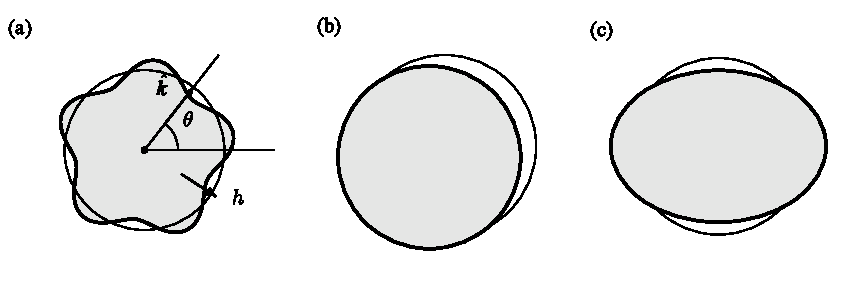
\includegraphics[width=0.72\textwidth]{fig_5.4.pdf}
\caption*{图 5.4\quad (a) 费米液体中的集体涨落可以用费米面的位移来描述。(b) $l=1$ 模式对应偶极涨落，(c) $l=2$ 模式对应四极涨落。}
\end{figure}

为简单起见，我们把讨论限制在二维系统，并且略去自旋指标。位移 $h$ 与占据数 $n_{\pmb{k}}$ 之间的关系如下：
\begin{equation*}
\tilde{\rho}(\theta) = \int \frac{k\,\mathrm{d}k}{(2\pi)^{2}}\, \delta n_{\pmb{k}=k\hat{\pmb{k}}}, \qquad h(\theta) = (2\pi)^{2} \tilde{\rho}(\theta)/k_F
\end{equation*}
其中 $\hat{\pmb{k}} = \cos(\theta)\pmb{x} + \sin(\theta)\pmb{y}$ 是 $\theta$ 方向的单位矢量（见图 5.4(a)）。结果表明 $\tilde{\rho}(\theta)$ 更为方便，所以下面我们用 $\tilde{\rho}$ 代替 $h$。由定义我们看到，$\int \mathrm{d}\theta\, \tilde{\rho}(\theta)$ 是电子总密度的涨落，对应于式 (5.1.2) 中的 $\rho$。

对于小涨落，$h$ 接近于零，准粒子能量 (5.3.3) 可以简化为
\begin{equation*}
\tilde{\epsilon}_{\pmb{k}}(\pmb{x},t) = \xi^{*}_{\pmb{k}} + \int \mathrm{d}\theta'\, f(\theta,\theta')\, \tilde{\rho}(\theta',\pmb{x},t) \tag{5.3.8}
\end{equation*}
其中 $\theta$ 是 $\pmb{k}$ 的方位角，$f(\theta,\theta') = f(k_F\hat{\pmb{k}}, k_F\hat{\pmb{k}}')$ 是费米面上两点之间的费米函数。对式 (5.3.7) 的两边施行积分 $\int \frac{k\,\mathrm{d}k}{(2\pi)^{2}}$，就得到约化玻尔兹曼方程。假定转动对称性，我们求得\footnote{注意 $\frac{\partial n}{\partial \pmb{k}} = -\hat{\pmb{k}}\,\delta(|\pmb{k}| - k_F) + \frac{\partial \delta n}{\partial \pmb{k}}$。我们发现
\begin{align*}
&\int \frac{k\,\mathrm{d}k}{(2\pi)^{2}}\, \hat{\pmb{k}}\, \delta(|\pmb{k}| - k_F) = \frac{k_F \hat{\pmb{k}}}{(2\pi)^{2}}\\
&\int \frac{k\,\mathrm{d}k}{(2\pi)^{2}} \left( \hat{\pmb{k}}_{\perp} k_F^{-1} \frac{\partial \delta n}{\partial \theta} + \hat{\pmb{k}} \frac{\partial \delta n}{\partial \pmb{k}} \right) = \hat{\pmb{k}}_{\perp} k_F^{-1} \frac{\partial \tilde{\rho}}{\partial \theta} - \int \frac{k\,\mathrm{d}k}{(2\pi)^{2}}\, k^{-1} \hat{\pmb{k}}\, \delta n = k_F^{-1} \left( \hat{\pmb{k}}_{\perp} \frac{\partial \tilde{\rho}}{\partial \theta} - \hat{\pmb{k}}\tilde{\rho} \right)
\end{align*}}
\begin{equation*}
\frac{\partial \tilde{\rho}}{\partial t} + \frac{\partial \tilde{\rho}}{\partial \pmb{x}} \cdot \frac{\partial \tilde{\epsilon}}{\partial \pmb{k}} + k_F^{-1} \left( \hat{\pmb{k}}_{\perp} \frac{\partial \tilde{\rho}}{\partial \theta} - \hat{\pmb{k}}\tilde{\rho} - \frac{\hat{\pmb{k}} k_F^{2}}{(2\pi)^{2}} \right) \cdot \left( \pmb{F} - \frac{\partial \tilde{\epsilon}}{\partial \pmb{x}} \right) = -\tau^{-1} \tilde{\rho} \tag{5.3.9}
\end{equation*}
其中 $\hat{\pmb{k}}_{\perp}$ 是与 $\hat{\pmb{k}}$ 垂直的单位矢量，$\tilde{\rho}$ 是函数 $\tilde{\rho}(\theta,\pmb{x},t)$。上式可以看作以 $(\theta,\pmb{x})$ 为参量的 $(1+2)$ 维空间中某个场的经典运动方程。线性化后的方程具有如下形式：
\begin{equation*}
\frac{\partial \tilde{\rho}}{\partial t} + v^{*}_F\, \hat{\pmb{k}} \cdot \frac{\partial \tilde{\rho}}{\partial \pmb{x}} - \frac{\hat{\pmb{k}} k_F}{(2\pi)^{2}} \cdot \left( \pmb{F} - \int \mathrm{d}\theta'\, f(\theta,\theta')\, \frac{\partial \tilde{\rho}(\theta',\pmb{x},t)}{\partial \pmb{x}} \right) = -\tau^{-1} \tilde{\rho} \tag{5.3.10}
\end{equation*}

当 $\pmb{F} = \tau^{-1} = 0$ 时，式 (5.3.10) 可以看作费米液体的一种运动方程，其形式为
\begin{equation*}
\frac{\partial \tilde{\rho}}{\partial t} + v^{*}_F\, \hat{\pmb{k}} \cdot \frac{\partial \tilde{\rho}}{\partial \pmb{x}} + \frac{k_F}{(2\pi)^{2}} \int \mathrm{d}\theta'\, f(\theta,\theta')\, \hat{\pmb{k}} \cdot \frac{\partial \tilde{\rho}(\theta',\pmb{x},t)}{\partial \pmb{x}} = 0 \tag{5.3.11}
\end{equation*}
相应的费米液体能量（或哈密顿量）(5.3.1) 也可以用 $\tilde{\rho}$ 写出：
\begin{align*}
H &= E_g + \int \mathrm{d}^{2}\pmb{x}\,\mathrm{d}\theta\; \tilde{\rho}\, \frac{h v^{*}_F}{2} + \frac{1}{2} \int \mathrm{d}^{2}\pmb{x}\,\mathrm{d}\pmb{k}\,\mathrm{d}\pmb{k}'\; f(\pmb{k},\pmb{k}')\, \delta n_{\pmb{k}} \delta n_{\pmb{k}'}\\
&= E_g + \int \mathrm{d}^{2}\pmb{x}\,\mathrm{d}\theta\; \frac{2\pi^{2} v^{*}_F}{k_F}\, \tilde{\rho}^{2} + \frac{1}{2} \int \mathrm{d}^{2}\pmb{x}\,\mathrm{d}\theta\,\mathrm{d}\theta'\; f(\theta,\theta')\, \tilde{\rho}(\theta) \tilde{\rho}(\theta') \tag{5.3.12}
\end{align*}
给出该运动方程与该哈密顿量的拉格朗日量为
\begin{align*}
L &= \int \mathrm{d}^{2}\pmb{x}\,\mathrm{d}\theta \left( \frac{1}{2k_F}\, \hat{\pmb{k}} \cdot \partial_{\pmb{x}} \tilde{\varphi}\, \partial_t \tilde{\varphi} - \frac{v^{*}_F}{2k_F}\, \big( \hat{\pmb{k}} \cdot \partial_{\pmb{x}} \tilde{\varphi} \big)^{2} \right)\\
&\quad - \frac{1}{8\pi^{2}} \int \mathrm{d}^{2}\pmb{x}\,\mathrm{d}\theta\,\mathrm{d}\theta'\; f(\theta,\theta')\, \hat{\pmb{k}} \cdot \partial_{\pmb{x}} \tilde{\varphi}(\theta,\pmb{x},t)\; \hat{\pmb{k}}' \cdot \partial_{\pmb{x}} \tilde{\varphi}(\theta',\pmb{x},t) \tag{5.3.13}
\end{align*}
其中 $\tilde{\varphi}$ 与 $\tilde{\rho}$ 通过 $\tilde{\rho}(\theta,\pmb{x},t) = (2\pi)^{-1} \hat{\pmb{k}} \cdot \frac{\partial \tilde{\varphi}(\theta,\pmb{x},t)}{\partial \pmb{x}}$ 相联系。式 (5.3.13) 是二维费米液体的一种流体动力学描述，换言之，是二维费米液体的一种玻色化。把它与 5.1.3 节讨论的流体动力学描述相比较，我们看到式 (5.3.13) 所包含的远不止密度模式。
\begin{figure}[H]
\centering
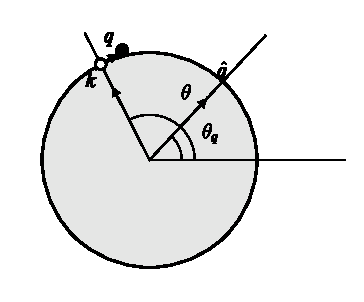
\includegraphics[width=0.72\textwidth]{fig_5.5.pdf}
\caption*{图 5.5\quad 动量为 $\pmb{q}$、位于角度 $\theta$ 处的粒子--空穴激发。}
\end{figure}

\subsection*{问题 5.3.3}

本节中我们为一个二维转动不变系统导出了约化玻尔兹曼方程及与之相联系的哈密顿量。把这些结果（式 (5.3.11) 与 (5.3.12)）推广到没有转动对称性的二维系统。

\subsection*{问题 5.3.4}

\begin{enumerate}
\item[(a)] 导出一维费米液体的玻色化拉格朗日量（即与式 (5.3.13) 类似的那个）。
\item[(b)] 在一维情形考虑式 (5.1.3)。通过 $\rho = (2\pi)^{-1}\partial_x \varphi$ 引入 $\varphi$。用 $\varphi$ 把式 (5.1.3) 写出来。求出 $\varphi$ 的正则动量（记作 $\tilde{\varphi}$），并用 $\varphi$ 与 $\tilde{\varphi}$ 表示哈密顿量 $H$。将作用量 $S = \int \mathrm{d}t\, (\tilde{\varphi}\dot{\varphi} - H)$ 与 (a) 中的结果比较。
\end{enumerate}

\subsection{费米液体流体动力学描述的应用}

作为费米液体玻色化描述的第一个应用，让我们计算集体模式的谱。在 $\pmb{q}$ 空间中，费米液体运动方程 (5.3.11) 变为
\begin{equation*}
\mathrm{i}\,\partial_t \tilde{\rho} = q \cos(\theta_{\pmb{q}} - \theta) \int \mathrm{d}\theta' \left( v^{*}_F \delta(\theta - \theta') + \frac{k_F}{(2\pi)^{2}} f(\theta,\theta') \right) \tilde{\rho}(\theta',\pmb{q},t) \tag{5.3.14}
\end{equation*}
其中 $\theta_{\pmb{q}}$ 是 $\pmb{q}$ 的方位角（见图 5.5）。

若 $f(\theta,\theta') = 0$，式 (5.3.14) 很容易求解。本征模具有形式 $\tilde{\rho}(\theta,\pmb{q},t) = \delta(\theta - \theta_0)\delta(\pmb{q} - \pmb{q}_0)\,\mathrm{e}^{-\mathrm{i}\omega(\pmb{q}_0,\theta_0)t}$，频率为 $\omega(\pmb{q}_0,\theta_0) = v^{*}_F q_0 \cos(\theta_{\pmb{q}_0} - \theta_0)$。这样的本征模描述一个动量为 $\pmb{q}_0$ 的激发。依赖于 $\theta$，这种激发的能量在 0 到 $v^{*}_F q_0$ 之间取值，
% 本块止于书页 212 末（句子未完）。p228 顶部 "agrees with the energy range of a
% particle–hole excitation of the same momentum (see Fig. 4.11)." 是本句下半句，
% 由 ch5_c 续译（"这与具有相同动量的粒子--空穴激发的能量范围一致（见图 4.11）。"）。

%--C-TAIL-- 两个电荷由于来自其他电子的屏蔽，并不感受到长程相互作用。

%JOIN%
与具有相同动量的粒子--空穴激发的能量范围一致（见图 4.11）。事实上，该本征模对应的正是图 5.5 中的粒子--空穴激发。

为求 $f(\theta,\theta')$ 非零时集体模式的能量，我们注意到式 (5.3.14) 可以改写为
\begin{equation*}
\mathrm{i}q^{-1}\partial_{t}\tilde{\rho}(\theta,\pmb{q},t)=KM\tilde{\rho}(\theta,\pmb{q},t) \tag{5.3.15}
\end{equation*}
其中两个实对称算符 $K$ 与 $M$ 由下式给出：
\begin{align*}
K(\theta,\theta') &= \cos(\theta_{\pmb{q}}-\theta)\,\delta(\theta-\theta')\\
M(\theta,\theta') &= v_{F}^{*}\,\delta(\theta-\theta')+\frac{k_{F}}{(2\pi)^{2}}f(\theta,\theta') \tag{5.3.16}
\end{align*}
由费米液体的能量（见式 (5.3.12)）可知，费米液体的稳定性要求 $M$ 是正定的。于是我们可以把 $M$ 写成 $M=\tilde{M}\tilde{M}^{\top}$。令 $u=\tilde{M}^{\top}\tilde{\rho}$，则式 (5.3.15) 变为 $\mathrm{i}\partial_{t}u=q\tilde{M}^{\top}K\tilde{M}u$。具有固定动量 $\pmb{q}$ 的集体激发，其能量由实对称矩阵 $q\tilde{M}^{\top}K\tilde{M}$ 的本征值给出。

转动对称性要求 $f(\theta,\theta')=f(\theta-\theta')$。由于能谱不依赖于 $\pmb{q}$ 的方向，我们可以取 $\pmb{q}$ 沿 $x$ 方向，即 $\pmb{q}=q\pmb{x}$、$\theta_{\pmb{q}}=0$。引入（见图 5.4）
\begin{equation*}
\tilde{\rho}_{l}(\pmb{q},t)=\int \mathrm{d}\theta\,\frac{\mathrm{e}^{-\mathrm{i}l\theta}}{\sqrt{2\pi}}\,\tilde{\rho}(\theta,\pmb{q},t),
\end{equation*}
式 (5.3.15) 便可写成
\begin{align*}
\mathrm{i}\partial_{t}\tilde{\rho}_{l}(q\pmb{x},t) &= qK_{lm}M_{ml'}\tilde{\rho}_{l'}(q\pmb{x},t), & f(\theta-\theta') &= \sum_{l}f_{l}\,\mathrm{e}^{\mathrm{i}l(\theta-\theta')},\\
K_{ll'} &= \frac{1}{2}\left(\delta_{l,l'+1}+\delta_{l,l'-1}\right), & M_{ll'} &= \left(v_{F}^{*}+\frac{k_{F}f_{l}}{2\pi}\right)\delta_{ll'}.
\end{align*}
由 $M$ 可见，若某一个 $f_{l}$ 小于 $-2\pi v_{F}^{*}/k_{F}$，费米液体就是不稳定的。我们还看到 $\tilde{M}_{ll'}\allowbreak=\sqrt{v_{F}^{*}+\frac{k_{F}f_{l}}{2\pi}}\,\delta_{ll'}$，以及
\begin{equation*}
q(\tilde{M}^{\top}K\tilde{M})_{ll'}\equiv\tilde{H}_{ll'}=\frac{q}{2}\left(\delta_{l,l'+1}+\delta_{l,l'-1}\right)\sqrt{v_{F}^{*}+\frac{k_{F}f_{l}}{2\pi}}\sqrt{v_{F}^{*}+\frac{k_{F}f_{l'}}{2\pi}}
\end{equation*}
$\tilde{H}$ 的本征值给出集体模式的频率。

这里 $\tilde{H}$ 描述一个在一维格子上跳跃的粒子。位点 $l$ 与位点 $l+1$ 之间的最近邻跳跃幅为
$\frac{q}{2}\sqrt{\frac{v_{F}^{*}}{2\pi}+\frac{k_{F}f_{l}}{(2\pi)^{2}}}\sqrt{\frac{v_{F}^{*}}{2\pi}+\frac{k_{F}f_{l+1}}{(2\pi)^{2}}}$。

\begin{figure}[H]
\centering
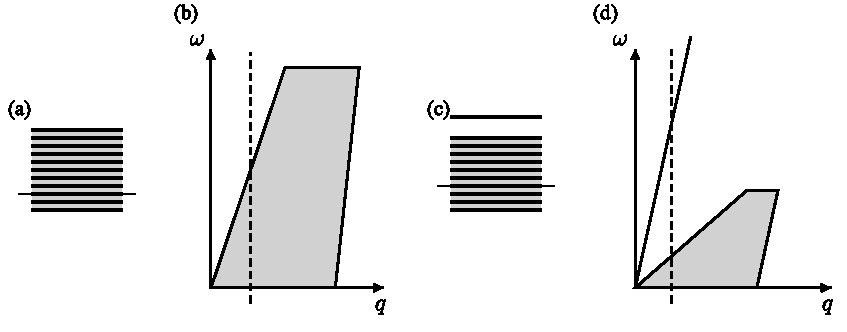
\includegraphics[width=0.72\textwidth]{fig_5.6.pdf}
\caption*{图 5.6\quad (a) $f_{l}=0$ 时 $\tilde{H}$ 的谱，(b) 相应的粒子--空穴谱。(c) $f_{l}>0$ 时 $\tilde{H}$ 的谱，(d) 相应的粒子--空穴谱。}
\end{figure}

当 $f_{l}=0$ 时，$\tilde{H}$ 具有从 $-v_{F}^{*}q$ 到 $v_{F}^{*}q$ 的连续谱（见图 5.6(a)），它重现了自由费米子系统的粒子--空穴连续谱（见图 5.6(b)）。然而，若 $f_{l}>f_{\infty}$，则由 $\tilde{H}_{ll'}$ 所描述的粒子会被吸引到小 $l$ 的区域。于是，除连续谱之外，$\tilde{H}$ 的谱中还有对应于吸引区内束缚态的孤立本征值（见图 5.6(c)）。相应的粒子--空穴谱则包含轮廓分明的集体模式（见图 5.6(d)）。\footnote{玻色型模式必须具有正能量，负能量意味着不稳定。然而，$\tilde{H}$ 既有正本征值也有负本征值，分别对应正、负频率。如果 $\tilde{H}$ 的正本征值对应玻色集体模式的正能量，那么 $\tilde{H}$ 的负本征值是否也对应集体模式的负能量？这里我们想指出，到目前为止我们一直是把式 (5.3.13) 当作经典拉格朗日量来处理的，也只讨论了由此得到的经典运动方程。量子化之后，运动方程变成关于算符 $\tilde{\rho}$ 的方程。事实表明，正频率的模式对应玻色模式的产生算符，而负频率的模式对应玻色模式的湮灭算符。式 (5.3.13) 的一维版本的量子化将在 7.4.5 节讨论，见式 (7.4.35) 与式 (7.4.36)。}

在第二个应用中，我们想用线性化的流体动力学运动方程 (5.3.10) 来计算费米液体的直流电导。当存在均匀的静态电场 $\pmb{E}$ 时，力由 $\pmb{F}=e\pmb{E}$ 给出。力 $\pmb{F}$ 将诱导出一个均匀且静态的 $\tilde{\rho}$，即 $\partial_{t}\tilde{\rho}=\partial_{\pmb{x}}\tilde{\rho}=0$。式 (5.3.10) 变为
\begin{equation*}
\tilde{\rho}=e\tau\,\frac{k_{F}}{(2\pi)^{2}}\,\hat{\pmb{k}}\cdot\pmb{E}
\end{equation*}
由式 (5.3.6) 可见，上述 $\tilde{\rho}$ 诱导出电流：
\begin{align*}
e\pmb{J} &= e\int \mathrm{d}\theta\,\tilde{\rho}\,\tilde{\pmb{v}}\\
\tilde{\pmb{v}}(\pmb{k}) &= \pmb{v}^{*}(\pmb{k})+\int \frac{\mathrm{d}^{2}\pmb{k}'}{(2\pi)^{2}}\,f(\pmb{k},\pmb{k}')\,\pmb{v}^{*}(\pmb{k}')\,\delta(\xi_{\pmb{k}'}^{*})
\end{align*}
由于转动对称性，$\tilde{\pmb{v}}=|\tilde{\pmb{v}}|\hat{\pmb{k}}$。我们得到
\begin{equation*}
e\pmb{J}=e^{2}\tau\,\frac{|\tilde{\pmb{v}}|k_{F}}{(2\pi)^{2}}\int \mathrm{d}\theta\,\hat{\pmb{k}}(\hat{\pmb{k}}\cdot\pmb{E})=\frac{e^{2}\tau|\tilde{\pmb{v}}|\rho}{k_{F}}\,\pmb{E}
\end{equation*}
电导为 $\sigma=\frac{e^{2}\tau|\tilde{\pmb{v}}|\rho}{k_{F}}$。若费米液体函数 $f(\pmb{k},\pmb{k}')$ 为零，上式就退化为 Drude 结果 $\sigma=\frac{e^{2}\tau\rho}{m^{*}}$。

\subsection*{问题 5.3.5}

当存在均匀磁场 $\pmb{B}=B\pmb{z}$ 时，二维约化玻尔兹曼方程 (5.3.9) 中的力 $\pmb{F}$ 具有 $\pmb{F}(\pmb{k},\pmb{x})=\frac{e}{c}\pmb{v}^{*}(\pmb{k})\times\pmb{B}$ 的形式。
\begin{enumerate}
\item[(a)] 证明：线性化之后，磁场中的约化玻尔兹曼方程在取 $\tau^{-1}=0$ 时具有如下形式（Kim et al., 1995）：
\begin{equation*}
\left(\mathrm{i}\partial_{t}+\mathrm{i}\omega_{c}\partial_{\theta}-v_{F}^{*}q\cos(\theta-\theta_{\pmb{q}})\right)\tilde{\rho}-\frac{qk_{F}\cos(\theta_{\pmb{q}}-\theta)}{(2\pi)^{2}}\int \mathrm{d}\theta'\,f(\theta-\theta')\,\tilde{\rho}(\theta',\pmb{q},t)=0
\end{equation*}
试求出 $\omega_{c}$。
\item[(b)] 证明：动量为 $\pmb{q}$ 的集体模式的能谱由下式的本征值决定：
\begin{equation*}
\tilde{H}_{ll'}=\omega_{c}l\,\delta_{ll'}+\frac{q}{2}\left(\delta_{l,l'+1}+\delta_{l,l'-1}\right)\sqrt{v_{F}^{*}+\frac{k_{F}f_{l}}{2\pi}}\sqrt{v_{F}^{*}+\frac{k_{F}f_{l'}}{2\pi}}
\end{equation*}
证明 $\tilde{H}$ 的谱关于零对称。（提示：$f_{l}=f_{-l}$ 为实数。）
\item[(c)] 证明：当 $f_{l}=0$ 时，$\tilde{H}$ 的本征值由 $\omega_{c}\times$ 整数给出。（提示：考虑 $\tilde{\rho}=\exp\bigl(\mathrm{i}l\theta-\mathrm{i}\frac{v_{F}^{*}q}{\omega_{c}}\sin(\theta-\theta_{\pmb{q}})\bigr)$。）这样我们便能用流体动力学理论恢复自由费米子的结果。
\end{enumerate}

\subsection*{问题 5.3.6}

\textbf{二维费米液体的交流输运}

\begin{enumerate}
\item[(a)] 设式 (5.3.9) 中的力 $\pmb{F}$ 具有 $\pmb{F}=e\pmb{E}\,\mathrm{e}^{\mathrm{i}\omega t-\pmb{q}\cdot\pmb{x}}$ 的形式。在 $f(\theta-\theta')=0$ 的假设下求 $\tilde{\rho}$。
\item[(b)] 准确到 $f(\theta-\theta')$ 的一阶，求 $\tilde{\rho}$。
\item[(c)] 求感应电流 $e\pmb{J}=\sigma(\omega,\pmb{q})\pmb{E}$，并准确到 $f(\theta-\theta')$ 的一阶求光学电导 $\sigma(\omega,\pmb{q})$。这里 $\pmb{J}$ 是式 (5.3.6) 给出的准粒子电流。
\end{enumerate}

\subsection{费米液体理论的本质}

人们通常认为，费米液体理论的精髓在于轮廓分明的准粒子这一概念及其实际存在。在 5.3.1 节中我们采纳的正是这一观点。轮廓分明的准粒子的存在意味着，不仅准粒子的总数守恒，而且在每个给定动量方向上的准粒子数目也守恒。于是，费米液体具有无穷多个守恒量（Luther, 1979; Haldane, 1992）。这使我们能够为费米液体建立一套流体动力学理论，其中包含许多玻色型模式，每个守恒量对应一个模式。因此，无穷多守恒量的存在也是费米液体理论的精髓之一。在 5.3.3 节中，我们正是基于这一观点建立了费米液体理论。

我们想指出，这两种观点并不等价，而且第二种观点更为普遍。轮廓分明的准粒子的存在意味着每个动量上的准粒子数目守恒；而在第二种观点中，我们只假设每个动量方向上的准粒子守恒。在一维情形，5.3.3 节的流体动力学理论实际上描述的是一维 Tomonaga--Luttinger 液体。\footnote{关于 Tomonaga--Luttinger 液体的讨论见 7.4.4 节。}在更高维数下，流体动力学理论描述的则是费米液体。

\section{微扰论与费米液体理论的有效性}

本节我们将检验费米液体理论的正确性。我们将发展一套微扰论来计算相互作用系统的电子格林函数，并检查 $\operatorname{Im}G(\pmb{k},\omega)$ 中是否含有 $\delta$ 函数。$\delta$ 函数的存在标志着轮廓分明的 Landau 准粒子的存在，也标志着 Landau 费米液体理论的适用。

\subsection{费米子的路径积分与微扰论}

\begin{keypoints}
\item 费米子的路径积分是一种记账形式体系，它使我们能够把费米子系统的关联函数形式地表达出来。与玻色子的路径积分不同，费米子路径积分的物理含义并不清楚。
\item 费米子的路径积分使我们能够为相互作用费米子系统系统地发展微扰论。
\item 微扰论的结构由费曼图与费曼规则所刻画。
\end{keypoints}

为建立费米子的路径积分，我们首先注意到，费米子算符的编时关联满足 $\langle T(c(t)c^{\dagger}(t'))\rangle=-\langle T(c^{\dagger}(t')c(t))\rangle$。于是，我们将用（复的）格拉斯曼数（Grassmann number）$\xi_{\alpha}$ 来表示费米子算符。读者可能会问，``用格拉斯曼数表示费米子算符''是什么意思？嗯，我不得不承认我不知道。我不知道格拉斯曼数的物理含义。我将把下面的费米子路径积分当作某种记账工具，它使我们能够把各种费米子关联函数形式地装进一个紧凑的公式里。格拉斯曼数是反对易数，满足
\begin{equation*}
\xi_{\alpha}\xi_{\beta}=-\xi_{\beta}\xi_{\alpha},\qquad \xi_{\alpha}\xi_{\beta}^{*}=-\xi_{\beta}^{*}\xi_{\alpha},\qquad \xi_{\alpha}^{2}=0,
\end{equation*}
以及
\begin{equation*}
\left(\xi_{\alpha_{1}}\dots\xi_{\alpha_{n}}\right)^{*}=\xi_{\alpha_{n}}^{*}\dots\xi_{\alpha_{1}}^{*}
\end{equation*}
格拉斯曼数的函数由如下展开定义：
\begin{equation*}
f(\xi)=f_{0}+f_{1}\xi,\qquad A(\xi,\xi^{*})=a_{0}+a_{1}\xi+\bar{a}_{1}\xi^{*}+a_{12}\xi^{*}\xi
\end{equation*}
导数的定义与普通导数相同，唯一的区别是：为了使导数算符 $\frac{\partial}{\partial\xi}$ 能作用到 $\xi$ 上，必须通过反对易把变量 $\xi$ 一路移到与 $\frac{\partial}{\partial\xi}$ 相邻的位置。例如，$\frac{\partial}{\partial\xi}(\xi^{*}\xi)=\frac{\partial}{\partial\xi}(-\xi\xi^{*})=-\xi^{*}$。在这些定义下，我们有
\begin{align*}
\frac{\partial}{\partial\xi}A(\xi,\xi^{*}) &= a_{1}-a_{12}\xi^{*}\\
\frac{\partial}{\partial\xi^{*}}A(\xi,\xi^{*}) &= \bar{a}_{1}+a_{12}\xi\\
\frac{\partial}{\partial\xi^{*}}\frac{\partial}{\partial\xi}A(\xi,\xi^{*}) &=-a_{12}=-\frac{\partial}{\partial\xi}\frac{\partial}{\partial\xi^{*}}A(\xi,\xi^{*})
\end{align*}
我们看到
\begin{equation*}
\frac{\partial}{\partial\xi^{*}}\frac{\partial}{\partial\xi}=-\frac{\partial}{\partial\xi}\frac{\partial}{\partial\xi^{*}}
\end{equation*}
格拉斯曼积分作为一种线性映射，被定义为格拉斯曼导数：
\begin{equation*}
\int \mathrm{d}\xi=\frac{\partial}{\partial\xi}
\end{equation*}
我们有
\begin{equation*}
\int \mathrm{d}\xi\,1=0,\qquad \int \mathrm{d}\xi\,\xi=1
\end{equation*}
格拉斯曼积分具有标准积分的如下性质：
\begin{equation*}
\int \mathrm{d}\xi\,\frac{\partial}{\partial\xi}f(\xi)=0,\qquad \int \mathrm{d}\xi\,f(\xi+\eta)=\int \mathrm{d}\xi\,f(\xi)
\end{equation*}
从行列式的定义
\begin{equation*}
\mathrm{Det}(H_{0})=\sum_{P}(-)^{P}(H_{0})_{1P_{1}}\dots(H_{0})_{nP_{n}}
\end{equation*}
（其中 $P$ 为置换 $(1,\dots,n)\to(P_{1},\dots,P_{n})$）出发，我们得到格拉斯曼高斯积分：
\begin{equation*}
\int \prod_{i=1}^{n}\mathrm{d}\eta_{i}^{*}\,\mathrm{d}\eta_{i}\,\mathrm{e}^{-\eta_{i}^{*}(H_{0})_{ij}\eta_{j}}=\mathrm{Det}(H_{0})
\end{equation*}
以及
\begin{equation*}
\int \prod_{i=1}^{n}\mathrm{d}\eta_{i}^{*}\,\mathrm{d}\eta_{i}\,\mathrm{e}^{-\eta_{i}^{*}(H_{0})_{ij}\eta_{j}+\zeta_{i}^{*}\eta_{i}+\zeta_{i}\eta_{i}^{*}}=\mathrm{Det}(H_{0})\,\mathrm{e}^{\zeta_{i}^{*}(H_{0}^{-1})_{ij}\zeta_{j}}
\end{equation*}
注意，与玻色型高斯积分相比，行列式出现在分子而不是分母中。

费米型高斯积分使我们能够得到（由路径积分定义的）费米子关联的 Wick 定理：
\begin{align*}
&\left\langle \psi_{1}\dots\psi_{n}\psi_{n}^{*}\dots\psi_{1}^{*}\right\rangle\\
&=\frac{\int \mathcal{D}\psi^{*}\mathcal{D}\psi\,\psi_{1}\dots\psi_{n}\psi_{n}^{*}\dots\psi_{1}^{*}\,\mathrm{e}^{-\sum_{ij}\psi_{i}^{*}(H_{0})_{ij}\psi_{j}}}{\int \mathcal{D}\psi^{*}\mathcal{D}\psi\,\mathrm{e}^{-\sum_{ij}\psi_{i}^{*}(H_{0})_{ij}\psi_{j}}}\\
&=\sum_{P}\zeta^{P}(H_{0}^{-1})_{P_{n},n}\dots(H_{0}^{-1})_{P_{1},1} \tag{5.4.1}
\end{align*}
其中 $\zeta=-1$。（若取 $\zeta=+1$，则上式便是玻色算符的 Wick 定理。）

让我们把上述形式体系应用于零温下的自由费米子系统。考虑如下路径积分：
\begin{align*}
Z_{0} &= \int \mathcal{D}\psi^{*}\mathcal{D}\psi\,\mathrm{e}^{\mathrm{i}\int_{0}^{\beta}\mathrm{d}t\,L_{0}}\\
L_{0} &= \sum_{\pmb{k}}\mathrm{i}\psi_{\pmb{k}}(t)^{*}\partial_{t}\psi_{\pmb{k}}(t)-\psi_{\pmb{k}}(t)^{*}\xi_{\pmb{k}}\psi_{\pmb{k}}(t)
\end{align*}
我们可以算出路径积分平均
\begin{equation*}
\mathrm{i}G_{\pmb{k}}(t,t')=\left\langle \psi_{\pmb{k}}(t)\psi_{\pmb{k}}^{*}(t')\right\rangle=\frac{1}{(-\mathrm{i})(\mathrm{i}\partial_{t}-\xi_{\pmb{k}})}
\end{equation*}
在频率空间中，我们有
\begin{equation*}
G_{\pmb{k},\omega}=\frac{1}{\omega-\xi_{\pmb{k}}}
\end{equation*}
它与式 (4.2.9) 中的编时平均\footnote{这里给出的计算是一种形式计算，未能重现重要的 $0^{+}$ 项。2.2.2 节讨论过如何产生 $0^{+}$ 项。}$\langle 0|T(\psi_{\pmb{k}}(t)\psi_{\pmb{k}}^{\dagger}(t'))|0\rangle$ 相一致。利用 Wick 定理，我们可以导出路径积分平均与编时平均之间如下更为普遍的关系：
\begin{equation*}
\left\langle \psi_{i_{1}}\dots\psi_{i_{n}}\psi_{j_{n}}^{*}\dots\psi_{j_{1}}^{*}\right\rangle=\frac{\mathrm{Tr}\left(T(\psi_{i_{1}}\dots\psi_{i_{n}}\psi_{j_{n}}^{\dagger}\dots\psi_{j_{1}}^{\dagger}\,\mathrm{e}^{-\int_{0}^{\beta}\mathrm{d}t\,H_{0}})\right)}{\mathrm{Tr}\left(T(\mathrm{e}^{-\int_{0}^{\beta}\mathrm{d}t\,H_{0}})\right)}
\end{equation*}
这样，我们就可以用路径积分计算任意的编时关联。

以上结果都是针对自由费米子系统的。让我们把路径积分应用于具有如下形式的相互作用系统：
\begin{equation*}
H=H_{0}+H_{I}(t)
\end{equation*}
其中 $H_{0}$ 描述自由费米子系统。设 $H_{I}(t)$ 是 $t$ 的缓变函数，在有限的 $t$ 处 $H_{I}(t)=H_{I}$，而 $H_{I}(\pm\infty)=0$。令
\begin{equation*}
Z=\left\langle 0\left|T\bigl(\mathrm{e}^{-\mathrm{i}\int \mathrm{d}t\,(H_{0}+H_{I}(t))}\bigr)\right|0\right\rangle
\end{equation*}
为配分函数，其中 $|0\rangle$ 是 $H_{0}$ 的基态。配分函数 $Z$ 有如下微扰展开：
\begin{align*}
Z &= Z_{0}\left(1+Z_{0}^{-1}\left\langle 0\left|T\left((- \mathrm{i}\int \mathrm{d}t\,H_{I})\,\mathrm{e}^{-\mathrm{i}\int \mathrm{d}t\,H_{0}}\right)\right|0\right\rangle+\dots\right)\\
Z_{0} &= \left\langle 0\left|T(\mathrm{e}^{-\mathrm{i}\int \mathrm{d}t\,H_{0}})\right|0\right\rangle.
\end{align*}
由于薛定谔绘景中的 $Z_{0}^{-1}\langle 0|T(O_{1}(t_{1})\dots\allowbreak O_{n}(t_{n})\,\mathrm{e}^{-\mathrm{i}\int \mathrm{d}t\,H_{0}})|0\rangle$ 等于海森堡绘景中的 $\langle 0|T(O_{1}(t_{1})\dots\allowbreak O_{n}(t_{n}))|0\rangle$，这两个量都表示编时平均。我们看到，相互作用系统的配分函数 $Z$ 可以用自由费米子系统 $H_{0}$ 中的编时平均表出。这使我们能够把 $Z$ 用路径积分表示如下：
\begin{equation*}
Z=\int \mathcal{D}\psi^{*}\mathcal{D}\psi\,\mathrm{e}^{\mathrm{i}\int_{0}^{\beta}\mathrm{d}t\,(L_{0}+L_{I})},\qquad L_{I}=-H_{I}
\end{equation*}
类似地，利用微扰展开可以证明，相互作用系统的（薛定谔绘景中的）编时关联可以用路径积分表示如下：
\begin{equation*}
\frac{\left\langle 0\left|T(O_{1}(t_{1})\dots O_{n}(t_{n})\,\mathrm{e}^{-\mathrm{i}\int \mathrm{d}t\,H})\right|0\right\rangle}{\left\langle 0\left|T(\mathrm{e}^{-\mathrm{i}\int \mathrm{d}t\,H})\right|0\right\rangle}=\frac{\int \mathcal{D}\psi^{*}\mathcal{D}\psi\,O_{1}(t_{1})\dots O_{n}(t_{n})\,\mathrm{e}^{\mathrm{i}\int_{0}^{\beta}\mathrm{d}t\,(L_{0}+L_{I})}}{\int \mathcal{D}\psi^{*}\mathcal{D}\psi\,\mathrm{e}^{\mathrm{i}\int_{0}^{\beta}\mathrm{d}t\,(L_{0}+L_{I})}}
\end{equation*}
现在，让我们用路径积分微扰地计算配分函数 $Z$：
\begin{align*}
Z &= Z_{0}\,\frac{\int \mathcal{D}\psi^{*}\mathcal{D}\psi\,\mathrm{e}^{\mathrm{i}\int \mathrm{d}t\,(L_{0}+L_{I})}}{\int \mathcal{D}\psi^{*}\mathcal{D}\psi\,\mathrm{e}^{\mathrm{i}\int \mathrm{d}t\,L_{0}}}\\
&=Z_{0}\left(1+\left\langle \left(\mathrm{i}\int \mathrm{d}t\,L_{I}\right)\right\rangle_{0}+\frac{1}{2!}\left\langle \left(\mathrm{i}\int \mathrm{d}t\,L_{I}\right)^{2}\right\rangle_{0}+\dots\right)
\end{align*}
若假设相互作用具有如下形式：
\begin{equation*}
\int \mathrm{d}t\,L_{I}=-\int \mathrm{d}x\,\mathrm{d}x'\,\psi^{*}(x^{\mu})\psi(x^{\mu})V(x^{\mu},x'^{\mu})\psi^{*}(x'^{\mu})\psi(x'^{\mu})
\end{equation*}

\begin{figure}[H]
\centering
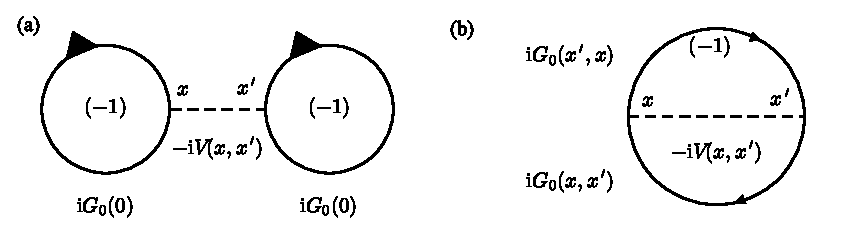
\includegraphics[width=0.72\textwidth]{fig_5.7.pdf}
\caption*{图 5.7\quad 对 $Z/Z_{0}$ 贡献 $V$ 一阶项的图。}
\end{figure}

其中 $x^{\mu}=(t,x^{1},\dots,x^{d})$，$\mathrm{d}x=\mathrm{d}t\,\mathrm{d}^{d}\pmb{x}$，那么我们发现
\begin{align*}
\frac{Z}{Z_{0}} &= 1+\left\langle \int \mathrm{d}x\,\mathrm{d}x'\,\psi^{*}(x^{\mu})\psi(x^{\mu})[-\mathrm{i}V(x^{\mu},x'^{\mu})]\psi^{*}(x'^{\mu})\psi(x'^{\mu})\right\rangle_{0}+\dots\\
&=1+\int \mathrm{d}x\,\mathrm{d}x'\,(-)\mathrm{i}G_{0}(0)[-\mathrm{i}V(x^{\mu},x'^{\mu})](-)\mathrm{i}G_{0}(0)\\
&\quad +\int \mathrm{d}x\,\mathrm{d}x'\,(-)\mathrm{i}G_{0}(x^{\mu}-x'^{\mu})\,\mathrm{i}G_{0}(x'^{\mu}-x^{\mu})[-\mathrm{i}V(x^{\mu},x'^{\mu})]+\dots
\end{align*}
$V$ 的两个一阶项可以用图 5.7 所示的费曼图来表示。下面关于费米子的费曼规则与玻色子的几乎完全相同，唯一的区别是每个闭合圈额外贡献一个 $-1$ 因子。
\begin{enumerate}
\item[(a)] 费曼图中的每条线代表一个传播子 $G_{0}(x,x')$，其中 $x$ 与 $x'$ 是该线两端两个顶点的坐标。
\item[(b)] 每个顶点代表对该顶点位置的一个积分 $\int \mathrm{d}x$。
\item[(c)] 每条虚线代表相互作用势 $-\mathrm{i}V(x,x')$。
\item[(d)] 每个闭合费米圈贡献一个 $-1$ 因子。
\item[(e)] 连通图的值由规则 (a)--(d) 给出，非连通图的值由连通子图的乘积给出。
\end{enumerate}
费曼图抓住了微扰展开的结构。它们不仅给出 $V$ 量级的项，还给出 $V^{2}$ 量级的项以及所有其他更高阶的项。

在 $Z/Z_{0}$ 的微扰展开中，路径积分平均 $\langle\dots\rangle_{0}$ 同时包含连通图与非连通图。我们可以用连链展开把 $Z/Z_{0}$ 的展开改写为
\begin{equation*}
\ln\frac{Z}{Z_{0}}=\sum_{n=0}^{\infty}\frac{1}{n!}\left\langle \left(\mathrm{i}\int \mathrm{d}t\,L_{I}\right)^{n}\right\rangle_{0c}=\left\langle \mathrm{e}^{\mathrm{i}\int \mathrm{d}t\,L_{I}}\right\rangle_{0c} \tag{5.4.2}
\end{equation*}
其中路径积分平均 $\langle\dots\rangle_{0c}$ 只包含连通图。

\subsection*{问题 5.4.1}

\begin{enumerate}
\item[(a)] 计算 $Z/Z_{0}$ 微扰展开中 $V^{2}$ 量级的项，并画出相应的费曼图。
\item[(b)] 计算 $\ln(Z/Z_{0})$ 微扰展开中 $V^{2}$ 量级的项，并画出相应的费曼图。
\end{enumerate}

\subsection{自能与两体相互作用}

现在我们可以对如下相互作用电子系统微扰地计算电子格林函数了：
\begin{equation*}
H=\sum_{\pmb{k}}\xi_{\pmb{k}}c_{\alpha\pmb{k}}^{\dagger}c_{\alpha\pmb{k}}+\frac{1}{2\mathcal{V}}\sum_{\pmb{k},\pmb{k}',\pmb{q}}c_{\alpha\pmb{k}}^{\dagger}c_{\alpha,\pmb{k}-\pmb{q}}\,V_{\pmb{q}}\,c_{\beta\pmb{k}'}^{\dagger}c_{\beta,\pmb{k}'+\pmb{q}}
\end{equation*}
编时格林函数由如下路径积分平均给出：
\begin{equation*}
\mathrm{i}G(\pmb{x},t)\delta_{\alpha\beta}=\frac{\int \mathcal{D}c\,\mathcal{D}c^{*}\,c_{\alpha}(\pmb{x},t)c_{\beta}^{*}(0,0)\,\mathrm{e}^{\mathrm{i}\int \mathrm{d}t\,L}}{\int \mathcal{D}c\,\mathcal{D}c^{*}\,\mathrm{e}^{\mathrm{i}\int \mathrm{d}t\,L}}\equiv\left\langle c_{\alpha}(\pmb{x},t)c_{\beta}^{*}(0,0)\right\rangle
\end{equation*}
这是针对相互作用电子的，其中
\begin{equation*}
L=\mathrm{i}c_{\alpha}^{*}\partial_{t}c_{\alpha}-H
\end{equation*}
是相互作用电子的拉格朗日量。注意，这里我们假设了 $\langle c_{\alpha}(\pmb{x},t)c_{\beta}^{*}(0,0)\rangle$ 在自旋转动下不变，因而它具有 $\mathrm{i}G(\pmb{x},t)\delta_{\alpha\beta}$ 的形式。

为计算 $\mathrm{i}G$，方便的做法是引入
\begin{equation*}
Z[\eta_{\alpha},\eta_{\alpha}^{*}]=\int \mathcal{D}c\,\mathcal{D}c^{*}\,\mathrm{e}^{\mathrm{i}\int \mathrm{d}t\,L+\int \mathrm{d}t\,\mathrm{d}^{d}\pmb{x}\,(\eta_{\alpha}c_{\alpha}^{*}+\eta_{\alpha}^{*}c_{\alpha})}
\end{equation*}
其中 $\eta(\pmb{x},t)$ 与 $\eta^{*}(\pmb{x},t)$ 同 $c(\pmb{x},t)$ 与 $c^{*}(\pmb{x},t)$ 一样，都是格拉斯曼数。我们看到
\begin{equation*}
\mathrm{i}G(\pmb{x},t)\delta_{\alpha\beta}=\frac{\partial}{\partial\eta_{\alpha}^{*}(\pmb{x},t)}\frac{\partial}{\partial\eta_{\beta}(0,0)}\ln Z[\eta_{\alpha},\eta_{\alpha}^{*}]
\end{equation*}
利用式 (5.4.2)，我们得到
\begin{align*}
\mathrm{i}G(\pmb{x},t)\delta_{\alpha\beta} &= \frac{\partial}{\partial\eta_{\alpha}^{*}(\pmb{x},t)}\frac{\partial}{\partial\eta_{\beta}(0,0)}\left\langle \mathrm{e}^{\mathrm{i}\int \mathrm{d}t\,L_{I}+\int \mathrm{d}t\,\mathrm{d}^{d}\pmb{x}\,(\eta_{\alpha}c_{\alpha}^{*}+\eta_{\alpha}^{*}c_{\alpha})}\right\rangle_{0c}\\
&=\left\langle c_{\alpha}(\pmb{x},t)c_{\beta}^{*}(0,0)\,\mathrm{e}^{\mathrm{i}\int \mathrm{d}t\,L_{I}}\right\rangle_{0c} \tag{5.4.3}
\end{align*}
这个公式为用费曼图计算相互作用电子的编时格林函数奠定了基础。

\begin{figure}[H]
\centering
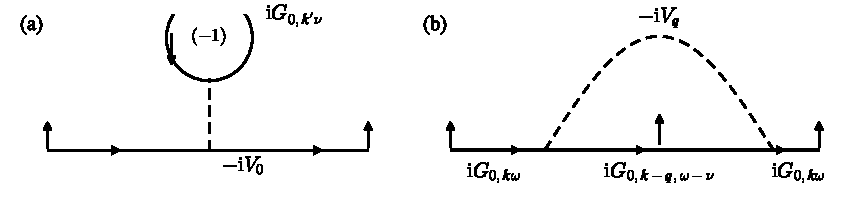
\includegraphics[width=0.72\textwidth]{fig_5.8.pdf}
\caption*{图 5.8\quad 对 $\mathrm{i}G_{\pmb{k}\omega}$ 有贡献的两个费曼图。虚线代表势 $-\mathrm{i}V_{\pmb{q}}$。}
\end{figure}

准确到 $V_{\pmb{q}}$ 的一阶，我们得到
\begin{equation*}
\mathrm{i}G(\pmb{x},t)\delta_{\alpha\beta}=\left\langle c_{\alpha}(\pmb{x},t)c_{\beta}^{\dagger}(0,0)\right\rangle_{0}+\left\langle c_{\alpha}(\pmb{x},t)c_{\beta}^{\dagger}(0,0)(-\mathrm{i})\int \mathrm{d}t'\,H_{I}(t')\right\rangle_{0c}
\end{equation*}
利用 Wick 定理，我们可以把上式用自由电子格林函数 $G_{0}$ 表出。在 $\pmb{k}$--$\omega$ 空间中，我们得到（见问题 5.4.2）
\begin{align*}
\mathrm{i}G_{\pmb{k}\omega} &= \mathrm{i}G_{0,\pmb{k}\omega}+(-1)(\mathrm{i}G_{0,\pmb{k}\omega})^{2}(-\mathrm{i}V_{0})\frac{1}{\mathcal{V}}\sum_{\pmb{k}',\alpha'}\int \frac{\mathrm{d}\nu}{2\pi}\,\mathrm{i}G_{0,\pmb{k}'\nu}\,\mathrm{e}^{\mathrm{i}0^{+}\nu}\\
&\quad +(\mathrm{i}G_{0,\pmb{k}\omega})^{2}\frac{1}{\mathcal{V}}\sum_{\pmb{q}}\int \frac{\mathrm{d}\nu}{2\pi}\,\mathrm{i}G_{0,\pmb{k}-\pmb{q},\nu}\,(-\mathrm{i}V_{\pmb{q}})\,\mathrm{e}^{-\mathrm{i}0^{+}\nu} \tag{5.4.4}
\end{align*}
其中自由电子格林函数 $G_{0,\pmb{k}\omega}$ 由式 (4.2.4) 给出。两个 $V_{\pmb{q}}$ 量级的项总结在图 5.8 所示的费曼图中。动量空间中的费曼规则与实空间中的不同，如下所示。
\begin{enumerate}
\item[(a)] 费曼图中的每条线携带一个能量--动量矢量，比如 $(\pmb{q},\nu)$。它代表一个传播子 $\mathrm{i}G_{\pmb{q}\nu}=\mathrm{i}/(\nu-\xi_{\pmb{q}})$。
\item[(b)] 流入一个节点的能量--动量是守恒的。
\item[(c)] 每个圈代表积分 $(\beta\mathcal{V})^{-1}\int \frac{\mathrm{d}\nu}{2\pi}\sum_{\pmb{q}}$（译注：原书误排为 $\mathrm{d}t$）。
\item[(d)] 虚线代表相互作用 $-\mathrm{i}V_{\pmb{q}}$，其中 $\pmb{q}$ 是流过虚线的动量。
\item[(e)] 由于费米子算符的反对易性质，每个闭合圈额外贡献一个 $-1$ 因子。（玻色系统的动量空间费曼规则没有这样的 $-1$ 因子。）
\end{enumerate}

式 (5.4.4) 可以写成
\begin{equation*}
\mathrm{i}G_{\pmb{k}\omega}=\mathrm{i}G_{0,\pmb{k}\omega}+(\mathrm{i}G_{0,\pmb{k}\omega})^{2}(-\mathrm{i}\Sigma_{\pmb{k}\omega})
\end{equation*}

\begin{figure}[H]
\centering
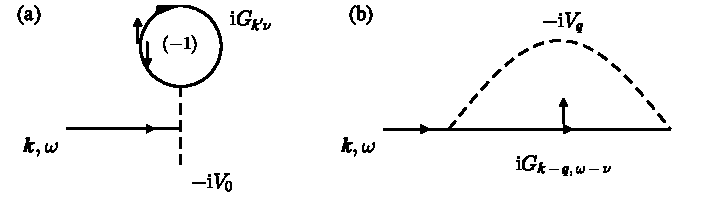
\includegraphics[width=0.72\textwidth]{fig_5.9.pdf}
\caption*{图 5.9\quad 对自能 $-\mathrm{i}\Sigma_{\pmb{k}\omega}$ 有贡献的两个图。}
\end{figure}

\begin{figure}[H]
\centering
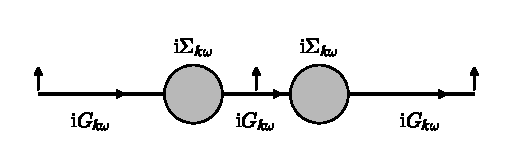
\includegraphics[width=0.72\textwidth]{fig_5.10.pdf}
\caption*{图 5.10\quad 对 $\mathrm{i}G_{\pmb{k}\omega}$ 有贡献的更高阶图。}
\end{figure}

其中
\begin{align*}
&-\mathrm{i}\Sigma_{\pmb{k}\omega}\\
&=(-1)\frac{-\mathrm{i}V_{0}}{\mathcal{V}}\sum_{\pmb{k}',\alpha'}\int \frac{\mathrm{d}\nu}{2\pi}\,\mathrm{i}G_{0,\pmb{k}'\nu}\,\mathrm{e}^{\mathrm{i}0^{+}\nu}+\frac{1}{\mathcal{V}}\sum_{\pmb{q}}\int \frac{\mathrm{d}\nu}{2\pi}\,\mathrm{i}G_{0,\pmb{k}-\pmb{q},\nu}\,(-\mathrm{i}V_{\pmb{q}})\,\mathrm{e}^{-\mathrm{i}0^{+}\nu}.
\end{align*}
上式可以用图 5.9 中的图来表示。如果我们把图 5.10 中的图所代表的某些更高阶项包括进来，格林函数就可以写成
\begin{equation*}
\mathrm{i}G_{\pmb{k}\omega}=\mathrm{i}G_{0,\pmb{k}\omega}\sum_{n=0}^{\infty}\left[(\mathrm{i}G_{0,\pmb{k}\omega})(-\mathrm{i}\Sigma_{\pmb{k}\omega})\right]^{n}
\end{equation*}
我们得到
\begin{equation*}
G_{\pmb{k}\omega}=\frac{1}{\omega-\xi_{\pmb{k}}-\Sigma_{\pmb{k}\omega}+\mathrm{i}\,\mathrm{sgn}(\omega)0^{+}}
\end{equation*}
色散关系既可以由 $G_{\pmb{k}\omega}$ 的极点位置得到，也可以由 $\omega-\xi_{\pmb{k}}-\Sigma_{\pmb{k}\omega}$ 的零点位置得到。我们看到，$\Sigma_{\pmb{k}\omega}$ 修正了电子（或准粒子）的能量，被称为自能。

注意
\begin{equation*}
\int \frac{\mathrm{d}\nu}{2\pi}\,\mathrm{i}G_{0,\pmb{k}'\nu}\,\mathrm{e}^{\mathrm{i}0^{+}\nu}=\mathrm{i}\int \frac{\mathrm{d}\nu}{2\pi}\,\frac{1}{\nu-\xi_{\pmb{k}'}+\mathrm{i}0^{+}\mathrm{sgn}(\nu)}\,\mathrm{e}^{\mathrm{i}0^{+}\nu}=-\Theta(-\xi_{\pmb{k}'})=-n_{\pmb{k}'}
\end{equation*}
由于围道必须在复 $\nu$ 平面的上半平面闭合，只有 $\nu$ 为负的极点才有贡献。由于 $\sum_{\pmb{k}',\alpha}\Theta(-\xi_{\pmb{k}'})$ 恰好就是电子的总数，自能中的第一项正是 Hartree 贡献（图 5.9(a)）：
\begin{equation*}
\Sigma_{\pmb{k}\omega}=V_{0}\rho_{0}+\dots
\end{equation*}
类似地，自能中的第二项（图 5.9(b)）具有如下形式：
\begin{equation*}
\Sigma_{\pmb{k}\omega}=\dots+\frac{1}{\mathcal{V}}\sum_{\pmb{q}}(-n_{\pmb{k}-\pmb{q}})V_{\pmb{q}}
\end{equation*}
这正是自能中的 Fock 贡献。

\begin{figure}[H]
\centering
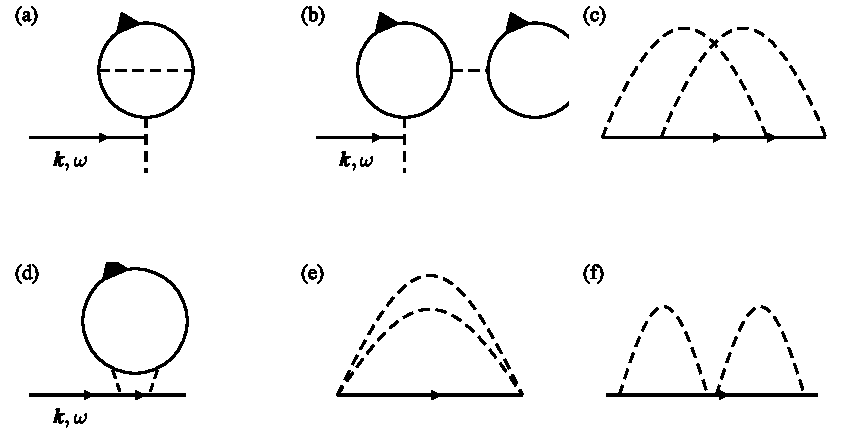
\includegraphics[width=0.72\textwidth]{fig_5.11.pdf}
\caption*{图 5.11\quad 图 (a)--(e) 对 $V_{\pmb{q}}^{2}$ 量级的自能有贡献。图 (f) 对自能没有贡献，因为它已包含在图 5.10 之中。}
\end{figure}

在上面，我们看到了如何从这些图计算自能 $\Sigma_{\pmb{k}\omega}$ 以及准粒子色散 $\xi_{\pmb{k}}^{*}=\xi_{\pmb{k}}+\Sigma_{\pmb{k}\omega}\big|_{\omega=\xi_{\pmb{k}}^{*}}$。这一做法在 $V$ 的一阶上重现了 Hartree--Fock 结果。而图方法还使我们能够以系统的方式计算自能的更高阶贡献（见图 5.11）。

我们还可以用图来计算费米液体理论中的费米液体函数。我们知道，相互作用 $V_{\pmb{q}}$ 可以把动量为 $\pmb{k}_{1}$ 和 $\pmb{k}_{2}$ 的两个电子散射为动量为 $\pmb{k}_{1}'$ 和 $\pmb{k}_{2}'$ 的两个电子。费米液体理论中的相互作用项 $n_{\pmb{k}_{1}}n_{\pmb{k}_{2}}V(\pmb{k}_{1}-\pmb{k}_{2})$ 对应于把动量为 $\pmb{k}_{1}$ 和 $\pmb{k}_{2}$ 的两个电子散射为具有相同动量的两个电子的那些项。于是，费米液体函数 $f$ 接收两个贡献，由图 5.12 中的两个图所示：
\begin{equation*}
-\mathrm{i}f(\pmb{k}_{1},\alpha;\pmb{k}_{2},\beta)=(-\mathrm{i}V_{0})+(-)(-\mathrm{i}V_{\pmb{q}})\delta_{\alpha\beta}
\end{equation*}

\begin{figure}[H]
\centering
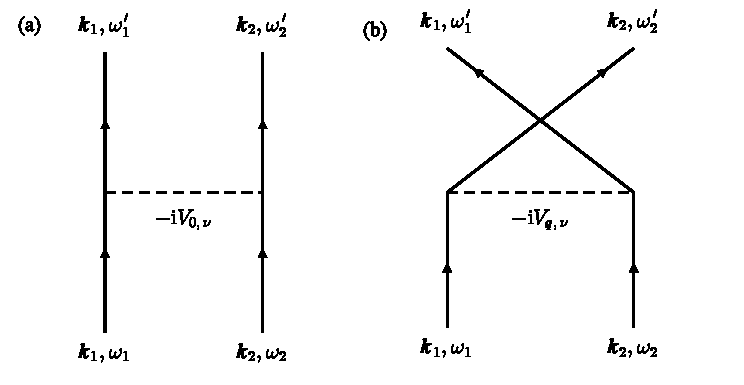
\includegraphics[width=0.72\textwidth]{fig_5.12.pdf}
\caption*{图 5.12\quad 对费米液体函数 $f(\pmb{k}_{1},\alpha;\pmb{k}_{2},\beta)$ 有贡献的图。(a) 这里 $\pmb{q}=\pmb{k}_{1}-\pmb{k}_{1}=0$ 是动量转移，$\nu=\omega_{1}-\omega_{1}'$ 是能量转移。(b) 这里 $\pmb{q}=\pmb{k}_{1}-\pmb{k}_{2}$ 是动量转移，$\nu=\omega_{1}-\omega_{2}'$ 是能量转移。}
\end{figure}

$(-)$ 号来自交换，而 $\delta_{\alpha\beta}$ 来自散射前后两个电子必须具有相同自旋这一要求。由于这里考虑的相互作用是瞬时的，$V_{\pmb{q}}$ 不依赖于能量转移 $\nu$（见图 5.12）。由此得到的费米液体函数 $f$ 也是瞬时的，且不依赖于能量转移 $\nu$：
\begin{equation*}
f(\pmb{k}_{1},\alpha;\pmb{k}_{2},\beta)=V_{0}-V_{\pmb{k}_{1}-\pmb{k}_{2}}\delta_{\alpha\beta}
\end{equation*}
这正是我们之前得到的 Hartree--Fock 结果 (5.3.2)。

\subsection*{问题 5.4.2}

用微扰论证明式 (5.4.4)。我们注意到，$\int \frac{\mathrm{d}\nu}{2\pi}\,\allowbreak\mathrm{i}G_{0,\pmb{k}'\nu}\,\allowbreak\mathrm{e}^{\mathrm{i}0^{+}\nu}$ 代表等时下的 $\langle c^{\dagger}c\rangle$，而 $\int \frac{\mathrm{d}\nu}{2\pi}\,\allowbreak\mathrm{i}G_{0,\pmb{k}'\nu}\,\allowbreak\mathrm{e}^{-\mathrm{i}0^{+}\nu}$ 代表等时下的 $\langle cc^{\dagger}\rangle$。

\subsection*{问题 5.4.3}

求自能 $\Sigma_{\pmb{k}\omega}$ 的微扰展开中 $V_{\pmb{q}}^{2}$ 量级各项的表达式，即图 5.11(a)--(e) 所描述的那些项。

\subsection{无规相位近似与有效势}

\begin{keypoints}
\item 粒子--空穴激发对相互作用势的屏蔽可以包含在无规相位近似（random phase approximation, RPA）之中。
\end{keypoints}

我们已经看到，在三维情形且相互作用为库仑相互作用时，Hartree--Fock 近似给出的自能在费米面附近是奇异的。这一奇异性导致无穷大的费米速度。奇异性来自库仑相互作用的长程势。短程相互作用不能产生任何奇异的自能。然而，我们知道，金属中的
两个电荷由于来自其他电子的屏蔽，并不感受到长程相互作用。因此，人们可能会怀疑 Hartree–Fock 关于发散费米速度这一结果的正确性；尤其是在认识到 Hartree–Fock 近似只包含直接相互作用、不含任何屏蔽效应之后，更会如此。

\begin{figure}[H]
\centering
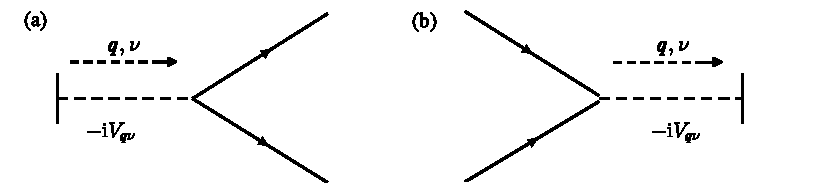
\includegraphics[width=0.72\textwidth]{fig_5.13.pdf}
\caption*{图 5.13\quad (a) 相互作用产生粒子–空穴激发；(b) 粒子–空穴激发修正相互作用。}
\end{figure}

\begin{figure}[H]
\centering
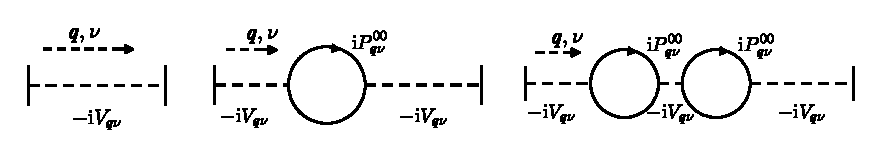
\includegraphics[width=0.72\textwidth]{fig_5.14.pdf}
\caption*{图 5.14\quad 无规相位近似下的有效势。}
\end{figure}

为了超越 Hartree–Fock 近似并把屏蔽效应包括进来，我们必须包括这样的效应：相互作用产生粒子–空穴激发（图 5.13(a)），而粒子–空穴激发又转而修正势（图 5.13(b)）。在无规相位近似（RPA）中，我们把图 5.14 中的图包括进来，如下计算屏蔽后的有效势：
\begin{equation*}
-\mathrm{i}V_{\pmb{q}\nu}^{\mathrm{eff}}=-\mathrm{i}V_{\pmb{q}\nu}\left(1+(-\mathrm{i}V_{\pmb{q}\nu})(\mathrm{i}P^{00}_{\pmb{q}\nu})+(-\mathrm{i}V_{\pmb{q}\nu})^{2}(\mathrm{i}P^{00}_{\pmb{q}\nu})^{2}+\cdots\right)
\end{equation*}
我们发现
\begin{equation*}
V_{\pmb{q}\nu}^{\mathrm{eff}}=\frac{V_{\pmb{q}\nu}}{1-V_{\pmb{q}\nu}P^{00}_{\pmb{q}\nu}}
\end{equation*}
在 $\nu\ll v_{F}q$ 极限下，$P^{00}_{\pmb{q}\nu}$ 等于压缩率的负值，即 $P^{00}_{\pmb{q}\nu}=-N(E_{F})$。我们有
\begin{equation*}
V_{\pmb{q}\nu}^{\mathrm{eff}}=\frac{V_{\pmb{q}\nu}}{1+V_{\pmb{q}\nu}N(E_{F})}
\end{equation*}
而对库仑相互作用，我们有
\begin{equation*}
V^{\mathrm{eff}}_{\pmb{q}}=\frac{4\pi e^{2}}{\pmb{q}^{2}+4\pi e^{2}N(E_{F})}
\end{equation*}

\begin{figure}[H]
\centering
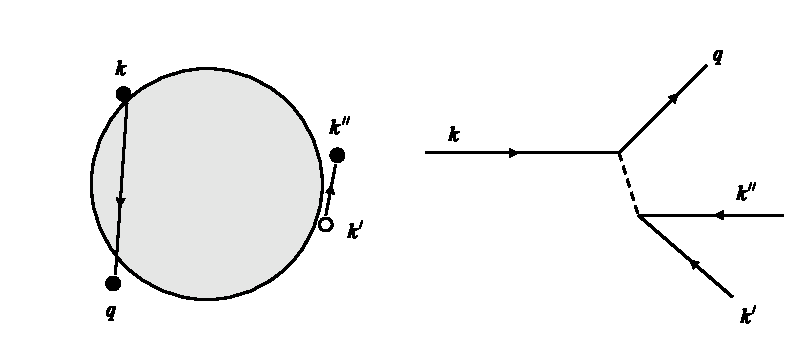
\includegraphics[width=0.72\textwidth]{fig_5.15.pdf}
\caption*{图 5.15\quad 准粒子的衰变。}
\end{figure}

显然，在 $\nu\ll v_{F}q$ 极限下，有效势在 $\pmb{q}\to 0$ 时并不奇异。这样的有效势代表一个屏蔽了的短程相互作用。同样的结果也可以通过 Thomas–Fermi 模型得到。

RPA 计算与屏蔽之间的关系可以按下面的方式看得更清楚。RPA 计算中的第一项（见图 5.14）代表两个不同位置处的两个密度（在图 5.14 中用两段短竖线表示）之间的直接（即未屏蔽的）相互作用。RPA 计算中的第二项代表这样的效应：一处的密度通过相互作用 $V_{\pmb{q}\nu}$ 诱导出一个粒子–空穴激发。该粒子–空穴激发代表一份形变了的密度，它转而与另一处的密度发生相互作用。通过这种方式，第二项（以及其他更高阶的项）修正或屏蔽了两个位置处的密度之间的相互作用。

在标准实践中，我们把裸势 $V_{\pmb{q}\nu}$ 换成屏蔽势 $V^{\mathrm{eff}}_{\pmb{q}\nu}=V_{\pmb{q}\nu}/(1+V_{\pmb{q}\nu}N(E_{F}))$，然后用这个有效势去计算自能与费米液体函数。在这一近似中，我们忽略了 $P^{00}$ 的频率依赖。一个瞬时的裸相互作用（不依赖频率的相互作用）被一个瞬时的有效相互作用所近似。如果把 $P^{00}$ 的频率依赖包括进来，那么一个瞬时的裸相互作用可以导致一个依赖频率的有效相互作用。这种频率依赖代表的正是推迟效应（retardation effects）。

\subsection{Landau 费米液体理论的论证}

\begin{keypoints}
\item 相互作用使准粒子发生衰变，但衰变率远小于准粒子的能量。Landau 费米液体理论尚待验证。
\end{keypoints}

一个电子–电子相互作用可以使动量为 $\pmb{k}$ 的电子衰变为一个动量为 $\pmb{q}$ 的电子加上一个动量为 $\pmb{k}-\pmb{q}$ 的粒子–空穴激发（见图 5.15）。粒子–空穴激发中的粒子与空穴各自可以具有 0 到 $\xi_{\pmb{k}}$ 之间的能量。$\pmb{q}$ 处粒子的能量会相应地调整以维持能量守恒。因此，可用衰变通道的数目正比于初始电子能量 $\xi_{\pmb{k}}$ 的平方。于是衰变率也正比于 $\xi^{2}_{\pmb{k}}$。由于衰变振幅正比于 $V_{\pmb{k}-\pmb{q}}$，我们求得衰变率为
\begin{equation*}
\Gamma_{\pmb{k}}\propto|V_{\pmb{k}}|^{2}\xi^{2}_{\pmb{k}}
\end{equation*}

\begin{figure}[H]
\centering
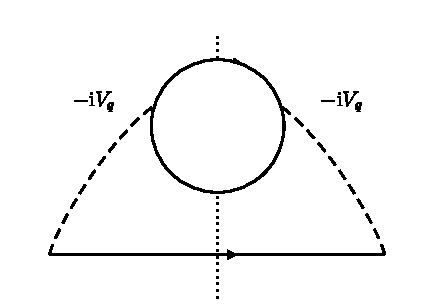
\includegraphics[width=0.72\textwidth]{fig_5.16.pdf}
\caption*{图 5.16\quad 对自能的 $V_{\pmb{q}}^{2}$ 量级的一项贡献。该图由两半构成，每一半代表图 5.15 中的衰变过程。上图给出衰变率，而图 5.15 中的图给出衰变振幅。}
\end{figure}

准粒子的衰变可以由自能的虚部来描述。当 $\Sigma_{\pmb{k}\omega}$ 具有虚部时，电子格林函数 $1/(\omega-\xi_{\pmb{k}}-\Sigma_{\pmb{k}\omega})$ 的极点就偏离实 $\omega$ 轴。这导致实时格林函数中的衰变：
\begin{equation*}
G(t,\pmb{k})=\int\frac{\mathrm{d}\omega}{2\pi}\,\frac{1}{\omega-\xi_{\pmb{k}}-\Sigma_{\pmb{k}\omega}}\,\mathrm{e}^{-\mathrm{i}\omega t}\sim\mathrm{e}^{-\mathrm{i}\xi^{*}_{\pmb{k}}t}\,\mathrm{e}^{-|\mathrm{Im}\Sigma_{\pmb{k}\xi^{*}_{\pmb{k}}}|t}
\end{equation*}
其中 $\xi^{*}_{\pmb{k}}=\xi_{\pmb{k}}+\mathrm{Re}\Sigma_{\pmb{k}\xi^{*}_{\pmb{k}}}$。我们看到自能的虚部由下式给出：
\begin{equation*}
|\mathrm{Im}\Sigma_{\pmb{k}\xi^{*}_{\pmb{k}}}|=\Gamma_{\pmb{k}}
\end{equation*}
我们想指出，这样的自能可以由图 5.16 中的费曼图得到。

由于衰变率 $\Gamma=\mathrm{Im}\Sigma_{\pmb{k}\xi^{*}_{\pmb{k}}}\propto(\xi^{*}_{\pmb{k}})^{2}$ 在低能极限下远小于准粒子能量 $\xi^{*}_{\pmb{k}}$，我们可以忽略准粒子的衰变。在这一极限下，准粒子激发可以被看作本征态。这就是 Landau 费米液体理论的基础。我们看到 $\mathrm{Im}G_{\pmb{k}\omega}$ 在 $\xi^{*}_{\pmb{k}}$ 处几乎是一个 $\delta$ 函数，峰的宽度仅正比于 $(\xi^{*}_{\pmb{k}})^{2}$。

在费米面附近我们可以使用展开
\begin{equation*}
\mathrm{Re}\Sigma_{\pmb{k}\omega}=\big(1-\frac{1}{Z}\big)\omega+\big(\frac{v^{*}_{F}}{Z}-v_{F}\big)(k-k_{F})
\end{equation*}
并把格林函数改写为
\begin{equation*}
G_{\pmb{k}\omega}=\frac{1}{\omega-v_{F}(k-k_{F})-\mathrm{Re}\Sigma_{\pmb{k}\omega}}=\frac{Z}{\omega-v^{*}_{F}(k-k_{F})}
\end{equation*}
这里 $Z$ 是 5.3.1 节末尾引入的交叠因子。这样，我们就在一个微扰计算之内论证了 Landau 费米液体理论。

\section{对称破缺相与自旋密度波态}

\begin{keypoints}
\item 费米液体可以有许多失稳。相互作用可以导致对称破缺相。
\end{keypoints}

相互作用费米子系统可以有许多不同的态，这些态造就了性质如此繁多的材料，例如超导体、磁体、电荷密度波态等等。材料的所有这些不同的态都可以理解为相互作用诱导的某些对称破缺态。本节中我们将只讨论其中一种对称破缺态——自旋密度波态。这里讨论的图像、方法与结果可以很容易地推广到其他对称破缺态，例如超导态。

\subsection{线性响应与失稳}

\begin{keypoints}
\item 一个具有如此众多无能隙激发的自由费米子系统，拥有许多潜在的失稳。费米子之间的相互作用可以把潜在的失稳变成真实的失稳。不同的相互作用诱导不同的失稳。
\end{keypoints}

考虑一个具有在位相互作用的格点电子系统：
\begin{align*}
H=&-\sum_{\langle ij\rangle,\alpha}t(c^{\dagger}_{\alpha j}c_{\alpha i}+\text{h.c.})-\mu N+U\sum_{i}n_{i}^{2}\\
=&-\sum_{\langle ij\rangle,\alpha}t(c^{\dagger}_{\alpha j}c_{\alpha i}+\text{h.c.})-\mu' N+U\sum_{i}c^{\dagger}_{\beta i}c^{\dagger}_{\alpha i}c_{\alpha i}c_{\beta i}\tag{5.5.1}
\end{align*}
其中 $n_{i}=\sum_{\alpha}c^{\dagger}_{\alpha i}c_{\alpha i}$ 是格点 $i$ 上的电子数，$N=\sum_{i}n_{i}$ 是电子总数。上述模型称为 Hubbard 模型。

下面我们将集中讨论二维的 Hubbard 模型。在动量空间中，二维 Hubbard 模型可以改写为
\begin{equation*}
H=\sum_{\pmb{k}}\xi_{\pmb{k}}c^{\dagger}_{\alpha\pmb{k}}c_{\alpha\pmb{k}}+U\frac{1}{N_{\mathrm{site}}}\sum_{\pmb{k},\pmb{k}',\pmb{q}}c^{\dagger}_{\alpha\pmb{k}}c^{\dagger}_{\beta\pmb{k}'}c_{\beta,\pmb{k}'+\pmb{q}}c_{\alpha,\pmb{k}-\pmb{q}}
\end{equation*}
其中
\begin{equation*}
\xi_{\pmb{k}}=-2t\left(\cos(k_{x})+\cos(k_{y})\right)-\mu'
\end{equation*}
$N_{\mathrm{site}}$ 是格点数目。我们注意到，当 $\mu'=0$ 时，费米海是半满的（$\langle n_{i}\rangle=1$），而且费米面是一个正方形（见图 5.17），它满足嵌套条件，嵌套波矢为 $\pmb{Q}=(\pi,\pi)$。由式 (4.3.3)，我们看到自由费米子在嵌套波矢 $\pmb{Q}$ 处的压缩率与自旋磁化率在低温下发散。由于态密度 $N(E_{F})$（这里 $N(E_{F})$ 指每格点每单位能量的态数）也具有对数发散，我们有

\begin{figure}[H]
\centering
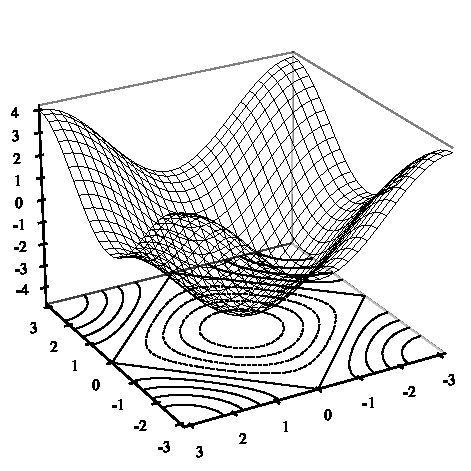
\includegraphics[width=0.72\textwidth]{fig_5.17.pdf}
\caption*{图 5.17\quad Hubbard 模型中的电子色散 $\xi_{\pmb{k}}$。}
\end{figure}

\begin{figure}[H]
\centering
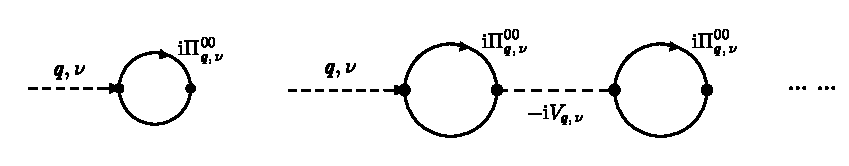
\includegraphics[width=0.72\textwidth]{fig_5.18.pdf}
\caption*{图 5.18\quad RPA 下的压缩率与自旋磁化率。}
\end{figure}

\begin{equation*}
\chi_{0}(\pmb{Q})\sim\frac{1}{E_{F}}\big(\ln\frac{E_{F}}{T}\big)^{2}\tag{5.5.2}
\end{equation*}
$T=0$ 处发散的 $\chi_{0}(\pmb{Q})$ 意味着系统正濒于产生密度序或自旋序。下面我们将证明，对于相互作用系统，当 $T$ 趋于一个有限的临界温度 $T_{c}$ 时，磁化率 $\chi(\pmb{Q})$ 发散。在 $T_{c}$ 以下，系统自发地产生电荷密度波（CDW）态或自旋密度波（SDW）态。

对于相互作用电子，压缩率与自旋磁化率会收到来自相互作用的修正。在 RPA 中，我们只考虑由图 5.18 中的图所描述的修正。单圈气泡图由如下关联给出：
\begin{equation*}
\left\langle \rho_{\alpha;\pmb{q}\nu}\rho_{\beta;-\pmb{q},-\nu}\right\rangle=\mathrm{i}\Pi^{00}_{\alpha\beta;\pmb{q}\nu}=\mathrm{i}\Pi^{00}_{\pmb{q}\nu}\delta_{\alpha\beta}
\end{equation*}

\begin{figure}[H]
\centering
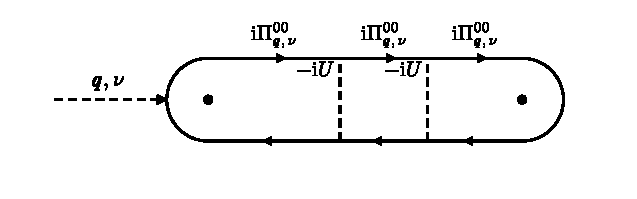
\includegraphics[width=0.72\textwidth]{fig_5.19.pdf}
\caption*{图 5.19\quad 对自旋与密度关联有贡献的梯形图。}
\end{figure}

而相互作用线由下式给出：
\begin{equation*}
-\mathrm{i}V_{\alpha\beta;\pmb{q}\nu}=-\mathrm{i}UC_{\alpha\beta}
\end{equation*}
其中 $\rho_{\alpha}$ 是自旋 $\alpha$ 电子的密度，$\pmb{C}=(C_{\alpha\beta})$ 是一个所有元素都等于 1 的 $2\times 2$ 矩阵。我们发现在 RPA 下，
\begin{align*}
\mathrm{i}\Pi^{\mathrm{RPA}}_{\alpha\beta;\pmb{q}\nu}&=\mathrm{i}\Pi^{00}_{\alpha\beta;\pmb{q}\nu}+\sum_{\gamma,\lambda}\mathrm{i}\Pi^{00}_{\alpha\gamma;\pmb{q}\nu}(-\mathrm{i}V_{\gamma\lambda;\pmb{q}\nu})\mathrm{i}\Pi^{00}_{\lambda\beta;\pmb{q}\nu}+\cdots\cdots\\
&=\sum_{\gamma}\mathrm{i}\Pi^{00}_{\pmb{q}\nu}\big(1-U\Pi^{00}_{\pmb{q}\nu}\pmb{C}\big)^{-1}_{\alpha\beta}=\mathrm{i}\Pi^{00}_{\pmb{q}\nu}\Big(\delta_{\alpha\beta}+\frac{U\Pi^{00}_{\pmb{q}\nu}}{1-2U\Pi^{00}_{\pmb{q}\nu}}C_{\alpha\beta}\Big)
\end{align*}
其中我们用到了 $(a+b\pmb{C})^{-1}=a^{-1}-b(a^{2}+2ab)^{-1}\pmb{C}$。于是，密度响应函数由下式给出：
\begin{align*}
\mathrm{i}\Pi^{\mathrm{RPA}}_{\mathrm{den};\pmb{q}\nu}&=\left\langle (\rho_{\uparrow;\pmb{q}\nu}+\rho_{\downarrow;\pmb{q}\nu})(\rho_{\uparrow;-\pmb{q},-\nu}+\rho_{\downarrow;-\pmb{q},-\nu})\right\rangle\\
&=\mathrm{i}\Pi^{\mathrm{RPA}}_{\uparrow\uparrow;\pmb{q}\nu}+\mathrm{i}\Pi^{\mathrm{RPA}}_{\downarrow\downarrow;\pmb{q}\nu}+2\,\mathrm{i}\Pi^{\mathrm{RPA}}_{\uparrow\downarrow;\pmb{q}\nu}=2\,\mathrm{i}\Pi^{00}_{\pmb{q}\nu}\frac{1}{1-2U\Pi^{00}_{\pmb{q}\nu}}
\end{align*}
而自旋响应函数由下式给出：
\begin{align*}
\mathrm{i}\Pi^{\mathrm{RPA}}_{\mathrm{spin};\pmb{q}\nu}&=\left\langle \frac{1}{2}(\rho_{\uparrow;\pmb{q}\nu}-\rho_{\downarrow;\pmb{q}\nu})\frac{1}{2}(\rho_{\uparrow;-\pmb{q},-\nu}-\rho_{\downarrow;-\pmb{q},-\nu})\right\rangle\\
&=\frac{1}{4}\,\mathrm{i}\Pi^{\mathrm{RPA}}_{\uparrow\uparrow;\pmb{q}\nu}+\frac{1}{4}\,\mathrm{i}\Pi^{\mathrm{RPA}}_{\downarrow\downarrow;\pmb{q}\nu}-\frac{1}{2}\,\mathrm{i}\Pi^{\mathrm{RPA}}_{\uparrow\downarrow;\pmb{q}\nu}=\frac{1}{2}\,\mathrm{i}\Pi^{00}_{\pmb{q}\nu}
\end{align*}

然而，上述结果并不十分完全。对于在位相互作用，图 5.19 中的梯形图与图 5.18 中的图有类似的贡献。把梯形图与气泡图的混合图包括进来，我们得到
\begin{align*}
\mathrm{i}\Pi^{\mathrm{RPA}^{+}}_{\alpha\beta;\pmb{q}\nu}&=\mathrm{i}\Pi^{00}_{\pmb{q}\nu}\delta_{\alpha\beta}+\sum_{\gamma\lambda}\left(\mathrm{i}\Pi^{00}_{\pmb{q}\nu}\delta_{\alpha\gamma}(-\mathrm{i}UC_{\gamma\lambda})\mathrm{i}\Pi^{00}_{\pmb{q}\nu}\delta_{\lambda\beta}\right)\\
&\quad+\sum_{\gamma\lambda}\left((-)\mathrm{i}\Pi^{00}_{\pmb{q}\nu}\delta_{\alpha\gamma}(-\mathrm{i}U\delta_{\gamma\lambda})\mathrm{i}\Pi^{00}_{\pmb{q}\nu}\delta_{\lambda\beta}\right)+\cdots\\
&=\sum_{\gamma}\mathrm{i}\Pi^{00}_{\pmb{q}\nu}\left(1-U\Pi^{00}_{\pmb{q}\nu}\pmb{C}+U\Pi^{00}_{\pmb{q}\nu}\right)^{-1}_{\alpha\beta}\\
&=\mathrm{i}\Pi^{00}_{\pmb{q}\nu}\left(\frac{1}{1+U\Pi^{00}_{\pmb{q}\nu}}\delta_{\alpha\beta}+\frac{U\Pi^{00}_{\pmb{q}\nu}}{1-(U\Pi^{00}_{\pmb{q}\nu})^{2}}C_{\alpha\beta}\right)
\end{align*}
新的密度响应函数由下式给出：
\begin{equation*}
\mathrm{i}\Pi^{\mathrm{RPA}^{+}}_{\mathrm{den};\pmb{q}\nu}=\mathrm{i}\Pi^{00}_{\pmb{q}\nu}\left(2\frac{1}{1+U\Pi^{00}_{\pmb{q}\nu}}+2\frac{U\Pi^{00}_{\pmb{q}\nu}}{1-(U\Pi^{00}_{\pmb{q}\nu})^{2}}+2\frac{U\Pi^{00}_{\pmb{q}\nu}}{1-(U\Pi^{00}_{\pmb{q}\nu})^{2}}\right)=2\,\frac{\mathrm{i}\Pi^{00}_{\pmb{q}\nu}}{1-U\Pi^{00}_{\pmb{q}\nu}}
\end{equation*}
新的自旋响应函数则由下式给出：
\begin{equation*}
\mathrm{i}\Pi^{\mathrm{RPA}^{+}}_{\mathrm{spin};\pmb{q}\nu}=\mathrm{i}\Pi^{00}_{\pmb{q}\nu}\left(2\frac{1}{1+U\Pi^{00}_{\pmb{q}\nu}}+2\frac{U\Pi^{00}_{\pmb{q}\nu}}{1-(U\Pi^{00}_{\pmb{q}\nu})^{2}}-2\frac{U\Pi^{00}_{\pmb{q}\nu}}{1-(U\Pi^{00}_{\pmb{q}\nu})^{2}}\right)=\frac{1}{2}\,\frac{\mathrm{i}\Pi^{00}_{\pmb{q}\nu}}{1+U\Pi^{00}_{\pmb{q}\nu}}
\end{equation*}
我们发现 RPA 下的压缩率 $\chi_{c}$ 与自旋磁化率 $\chi_{s}$ 由下式给出：
\begin{align*}
\chi^{\mathrm{RPA}^{+}}_{c}(\pmb{q})&=\frac{\chi^{(0)}_{c}(\pmb{q})}{1+\frac{1}{2}U\chi^{(0)}_{c}(\pmb{q})}\\
\chi^{\mathrm{RPA}^{+}}_{s}(\pmb{q})&=\frac{\chi^{(0)}_{s}(\pmb{q})}{1-2U\chi^{(0)}_{s}(\pmb{q})}
\end{align*}
其中 $\chi^{(0)}_{c}(\pmb{q})=-2\Pi^{00}_{\pmb{q},0}$ 与 $\chi^{(0)}_{s}(\pmb{q})=-\Pi^{00}_{\pmb{q},0}/2$ 是自由电子的压缩率与自旋磁化率。

我们看到，（短程的）排斥相互作用增强自旋磁化率而压制电荷压缩率，而（短程的）吸引相互作用压制自旋磁化率而增强电荷压缩率。对于嵌套费米面与排斥相互作用，当 $T$ 趋于由 $1-U\chi^{(0)}_{s}(\pmb{Q})=0$ 决定的有限临界温度 $T_{c}$ 时，$\chi^{\mathrm{RPA}^{+}}_{s}(\pmb{Q})$ 发散。在 $T_{c}$ 以下，系统自发地产生 SDW，并自发破缺自旋转动对称性与格子的平移对称性。转变温度可以由 $\chi^{(0)}_{s}(\pmb{Q})$ 的低温行为（见式 (5.5.2)）来估计：
\begin{equation*}
T_{c}\sim E_{F}\,\mathrm{e}^{-C_{1}\sqrt{\frac{E_{F}}{U}}}
\end{equation*}
我们看到，对于嵌套费米面，无论相互作用多么弱，排斥相互作用总会产生 SDW。同样，对于嵌套费米面，无论相互作用多么弱，吸引相互作用总会产生 CDW。转变温度为
\begin{equation*}
T_{c}\sim E_{F}\,\mathrm{e}^{-C_{2}\sqrt{\frac{E_{F}}{-U}}}
\end{equation*}

\subsection{自旋密度波态的平均场方法}

\begin{keypoints}
\item 在平均场方法中，我们把费米子算符的对换成它们的基态平均值，从而把一个相互作用的哈密顿量变成一个无相互作用的哈密顿量（平均场哈密顿量）。
\end{keypoints}

我们已经看到，具有嵌套费米面的系统中的排斥相互作用可能引起 SDW 失稳。在本节与接下来的几节中，我们将研究这种系统的基态，并证明基态的确具有 SDW 序。我们将使用两种方法，即平均场方法与变分方法。变分方法在概念上更简单也更正确，它还能计算准粒子之间的相互作用。平均场方法则在数学上更简单。我们先考虑平均场方法。

\begin{figure}[H]
\centering
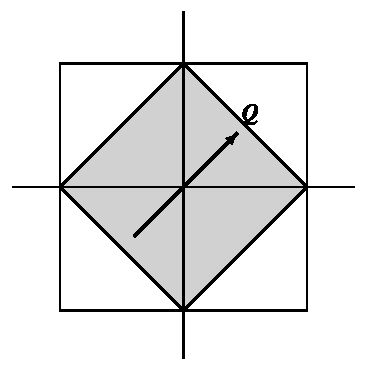
\includegraphics[width=0.72\textwidth]{fig_5.20.pdf}
\caption*{图 5.20\quad 阴影区域是约化布里渊区。它也是半满填充时被填满的费米海。}
\end{figure}

为了用平均场方法研究 $T=0$ 的 SDW 态，我们先把哈密顿量改写成更方便的形式。利用恒等式
\begin{equation*}
Un^{2}_{i}=-U(c^{\dagger}_{i}\sigma^{z}c_{i})^{2}+2Un_{i}
\end{equation*}
并把 $2Un_{i}$ 项吸收进化学势项中，我们可以把 Hubbard 模型改写为
\begin{equation*}
H=\sum_{\pmb{k},\alpha}\xi_{\pmb{k}}c^{\dagger}_{\alpha\pmb{k}}c_{\alpha\pmb{k}}-U\sum_{\pmb{i}}(c^{\dagger}_{\pmb{i}}\sigma^{z}c_{\pmb{i}})^{2}
\end{equation*}
现在我们可以形式地得到一个平均场哈密顿量：把自旋 $c^{\dagger}_{i}\sigma^{z}c_{i}$ 之一换成它的平均值 $(-)^{i}M$，并把 $(c^{\dagger}_{i}\sigma^{z}c_{i})^{2}$ 换成 $2M(-)^{i}(c^{\dagger}_{i}\sigma^{z}c_{i})-M^{2}$。我们得到
\begin{equation*}
H^{\mathrm{sub}}_{\mathrm{mean}}=\sum_{k,\alpha}\xi_{k}c^{\dagger}_{\alpha k}c_{\alpha k}-2U\sum_{i}(-)^{i}Mc^{\dagger}_{i}\sigma^{z}c_{i}+N_{\mathrm{site}}UM^{2}
\end{equation*}
在平均场近似下，我们说系统的物理性质由 $H^{\mathrm{sub}}_{\mathrm{mean}}$ 而不是原来的相互作用哈密顿量 (5.5.1) 描述。

平均场哈密顿量可以精确求解。在动量空间中，我们有
\begin{align*}
H^{\mathrm{sub}}_{\mathrm{mean}}&=\sum_{\pmb{k},\alpha}2t(\cos k_{x}+\cos k_{y})c^{\dagger}_{\pmb{k}}c_{\pmb{k}}-B\sum_{\pmb{k}}(-)^{i}c^{\dagger}_{\pmb{k}+\pmb{Q}}\sigma^{z}c_{\pmb{k}}+\text{常数}\\
&=\sum_{\pmb{k}}'\psi^{\dagger}_{\pmb{k}}M_{\pmb{k}}\psi_{\pmb{k}}+\text{常数}
\end{align*}
（译注：第二行中求和号后的 $(-)^{i}$ 为原书排印如此；交错相位因子在过渡到动量空间时已并入下面的 $\psi_{\pmb{k}}$ 与 $M_{\pmb{k}}$ 的定义。）其中 $B=2UM$，$\sum'_{\pmb{k}}$ 表示对约化布里渊区（见图 5.20）求和，$(-)^{i}=(-)^{i_{x}+i_{y}}$，
\begin{equation*}
M_{\pmb{k}}=\begin{pmatrix}\xi_{\pmb{k}} & -B\sigma^{z}\\ -B\sigma^{z} & -\xi_{\pmb{k}}\end{pmatrix},\qquad \xi_{\pmb{k}}=2t(\cos k_{x}+\cos k_{y})\tag{5.5.3}
\end{equation*}
而
\begin{equation*}
\psi_{\alpha\pmb{k}}=\begin{pmatrix}c_{\alpha\pmb{k}}\\ c_{\alpha,\pmb{k}+\pmb{Q}}\end{pmatrix}
\end{equation*}
我们可以通过引入
\begin{align*}
\eta_{\alpha\pmb{k}}&=-v_{\pmb{k}}\sigma^{z}_{\alpha\beta}c_{\beta\pmb{k}}+u_{\pmb{k}}c_{\alpha,\pmb{k}+\pmb{Q}}\\
\lambda_{\alpha\pmb{k}}&=u_{\pmb{k}}c_{\alpha\pmb{k}}+v_{\pmb{k}}\sigma^{z}_{\alpha\beta}c_{\beta,\pmb{k}+\pmb{Q}}
\end{align*}
来对角化上述平均场哈密顿量 $H^{\mathrm{sub}}_{\mathrm{mean}}$，其中
\begin{equation*}
u_{\pmb{k}}=\frac{1}{\sqrt{2}}\sqrt{1-\frac{\xi_{\pmb{k}}}{\sqrt{\xi^{2}_{\pmb{k}}+B^{2}}}}\qquad v_{\pmb{k}}=\mathrm{sgn}(B)\frac{1}{\sqrt{2}}\sqrt{1+\frac{\xi_{\pmb{k}}}{\sqrt{\xi^{2}_{\pmb{k}}+B^{2}}}}
\end{equation*}
由于 $u^{2}_{\pmb{k}}+v^{2}_{\pmb{k}}=1$，$\eta_{\alpha\pmb{k}}$ 与 $\lambda_{\alpha\pmb{k}}$ 满足费米子算符的下列对易关系：
\begin{align*}
\{\eta_{\alpha\pmb{k}},\eta^{\dagger}_{\alpha\pmb{k}'}\}&=\delta_{\pmb{k}\pmb{k}'}\delta_{\alpha\alpha'}\\
\{\lambda_{\alpha\pmb{k}},\lambda^{\dagger}_{\alpha\pmb{k}'}\}&=\delta_{\pmb{k}\pmb{k}'}\delta_{\alpha\alpha'}\\
\{\eta_{\alpha\pmb{k}},\lambda^{\dagger}_{\alpha\pmb{k}'}\}&=0
\end{align*}
用 $\eta_{\alpha\pmb{k}}$ 与 $\lambda_{\alpha\pmb{k}}$ 表示，我们得到
\begin{equation*}
H^{\mathrm{sub}}_{\mathrm{mean}}=\sum'_{\alpha,\pmb{k}}E_{\pmb{k}}\eta^{\dagger}_{\alpha\pmb{k}}\eta_{\alpha\pmb{k}}+\sum'_{\alpha,\pmb{k}}-E_{\pmb{k}}\lambda^{\dagger}_{\alpha\pmb{k}}\lambda_{\alpha\pmb{k}}+N_{\mathrm{site}}UM^{2}
\end{equation*}
而
\begin{equation*}
E_{\pmb{k}}=\sqrt{\xi^{2}_{\pmb{k}}+B^{2}}
\end{equation*}
我们可以看到，平均场基态能量由下式给出：
\begin{equation*}
E_{\mathrm{mean}}=-2\sum'_{\pmb{k}}E_{\pmb{k}}+N_{\mathrm{site}}\frac{B^{2}}{4U}
\end{equation*}
用平均场理论，准粒子激发的谱由 $\pm E_{\pmb{k}}$ 给出。

然而，上述平均场结果包含一个未知参量 $M$——交错自旋的平均值。为了确定 $M$，我们使平均场基态能量 $E_{\mathrm{mean}}$ 取极小。我们得到
\begin{equation*}
\frac{1}{4}-UN^{-1}_{\mathrm{site}}\sum'_{\pmb{k}}\frac{1}{E_{\pmb{k}}}=0.\tag{5.5.4}
\end{equation*}
这个方程称为能隙方程。通过施加自洽关系
\begin{equation*}
M=(-)^{i}\langle \Phi_{\mathrm{mean}}|c^{\dagger}_{i}\sigma^{z}c_{i}|\Phi_{\mathrm{mean}}\rangle
\end{equation*}
我们也可以得到同一个能隙方程，其中 $|\Phi_{\mathrm{mean}}\rangle$ 是 $H^{\mathrm{sub}}_{\mathrm{mean}}$ 的基态。也就是说，由平均场基态得到的平均自旋应当等于我们在得到平均场哈密顿量时所假设的平均自旋。

如果能隙方程有 $M\neq 0$ 的解，那么我们这个相互作用系统的基态就自发破缺自旋转动对称性，并发展出反铁磁序。由于 $\int\frac{\mathrm{d}^{2}k}{(2\pi)^{2}}\frac{1}{E_{k}}$ 在 $B\to 0$ 时趋于无穷，我们发现只要 $U>0$，式 (5.5.4) 总有 $M\neq 0$ 的解。于是，正 $U$ 的 Hubbard 模型总会发展出 SDW，无论 $U$ 多么小。这与上一节得到的结果一致。

我们想指出，只要 $\xi_{\pmb{k}}=-\xi_{\pmb{k}+\pmb{Q}}$，上述结果就仍然成立。在这种情形下，费米面（即 $\xi_{\pmb{k}}=0$ 处）上不同的点由 $\pmb{Q}$ 相连；换言之，费米面满足嵌套条件。对于更一般的 $\xi_{\pmb{k}}$，即费米面不满足嵌套条件的情形，准粒子的色散由下式给出：
\begin{equation*}
\pm\sqrt{\frac{1}{4}(\xi_{\pmb{k}}-\xi_{\pmb{k}+\pmb{Q}})^{2}+B^{2}}+\frac{1}{2}(\xi_{\pmb{k}}+\xi_{\pmb{k}+\pmb{Q}})
\end{equation*}
在这种情形下，能隙方程 (5.5.4) 不再适用。事实表明，$U$ 较小时并不会形成 SDW。

虽然平均场方法（以及下面讨论的变分方法）正确地重现了排斥型 Hubbard 模型的反铁磁基态，但由此得到的激发谱却是不正确的。这是因为反铁磁基态自发破缺了自旋转动对称性，基态之上应当存在无能隙的自旋波激发。自旋波激发可以通过自旋关联 $\mathrm{i}S^{ab}(i-j)=\left\langle (c^{\dagger}_{i}\sigma^{a}c_{i})(c^{\dagger}_{j}\sigma^{b}c_{j})\right\rangle$ 来探测。在平均场理论中，我们有 $S^{ab}\sim\delta_{ab}G^{2}_{\mathrm{mean}}$，其中 $G_{\mathrm{mean}}$ 是由 $H_{\mathrm{mean}}$ 确定的电子格林函数。于是，只有当 $|\omega|>2\Delta$ 时 $\mathrm{Im}S^{ab}_{\pmb{k}\omega}$ 才非零。然而，如果我们超越平均场理论，用 RPA 以及图 5.18 与图 5.19 中的梯形图来计算 $S^{ab}$，那么 $\mathrm{Im}S^{ab}_{\pmb{k}\omega}$ 将一直到 $\omega=0$ 都非零，这表明存在无能隙激发。此外，$S^{ab}_{\pmb{k}\omega}$ 还有一个孤立极点，由它我们可以得到自旋波激发的色散。

\subsection{自旋密度波态的变分方法——艰难的途径}

\begin{keypoints}
\item 在变分方法中，我们用一个无相互作用哈密顿量的基态作为尝试波函数，去近似一个相互作用哈密顿量的基态。
\end{keypoints}

在变分方法中，我们关注的是基态波函数，而不是哈密顿量。我们已经看到，具有在位排斥相互作用的 Hubbard 模型有 SDW 失稳。为了用变分方法理解基态的性质，我们索性为基态猜测一个尝试波函数。一个可能的选择是像我们在 Hartree–Fock 近似中所做的那样，使用 $H_{0}=\sum_{\pmb{k},\alpha}\tilde{\xi}_{\pmb{k}}c^{\dagger}_{\alpha\pmb{k}}c_{\alpha\pmb{k}}$ 的基态 $|\Psi_{0}\rangle$ 作为尝试波函数。然而，$|\Psi_{0}\rangle$ 并不破缺自旋与平移对称性。SDW 失稳的存在提示我们，应当能够找到一个能量更低的不同的尝试波函数。从对称性的考虑出发，我们愿意使用
\begin{equation*}
H_{B}=\sum_{\pmb{k},\alpha}2\tilde{t}(\cos k_{x}+\cos k_{y})c^{\dagger}_{\alpha\pmb{k}}c_{\alpha\pmb{k}}-B\sum_{i}(-)^{i}c^{\dagger}_{i}\sigma^{z}c_{i}
\end{equation*}
的基态 $|\Psi_{B}\rangle$ 作为尝试波函数。我们并不显式写出多体尝试波函数，而是像在平均场方法中那样，先对角化"变分"哈密顿量 $H_{B}$。$H_{B}$ 的基态满足 $\lambda^{\dagger}_{\alpha\pmb{k}}|\Psi_{B}\rangle=\eta_{\alpha\pmb{k}}|\Psi_{B}\rangle=0$。这一代数关系确定了我们的尝试波函数。

注意，哈密顿量 $H_{B}$ 只是用来得到尝试波函数的一个算符。把 $H_{B}$ 缩放一个常数不会改变尝试波函数。因此我们可以令 $\tilde{t}=t$，从而 $\tilde{\xi}_{\pmb{k}}=\xi_{\pmb{k}}$。此时 $H_{B}$ 与平均场哈密顿量 $H^{\mathrm{sub}}_{\mathrm{mean}}$ 具有相同的形式。这里 $B$ 是一个改变波函数形状的变分参量，我们稍后将改变 $B$ 使能量极小。

为了计算尝试态的平均能量，我们注意到，对于尝试波函数 $|\Psi_{B}\rangle$，我们有 $\langle\eta^{\dagger}_{\alpha\pmb{k}}\eta_{\alpha\pmb{k}}\rangle=0$ 与 $\langle\lambda^{\dagger}_{\alpha\pmb{k}}\lambda_{\alpha\pmb{k}}\rangle=1$。由
\begin{equation*}
c_{\alpha\pmb{k}}=u_{\pmb{k}}\lambda_{\alpha\pmb{k}}-v_{\pmb{k}}\sigma^{z}_{\alpha\beta}\eta_{\beta\pmb{k}}\qquad c_{\alpha,\pmb{k}+\pmb{Q}}=v_{\pmb{k}}\sigma^{z}_{\alpha\beta}\lambda_{\beta\pmb{k}}+u_{\pmb{k}}\eta_{\alpha\pmb{k}}
\end{equation*}
我们发现
\begin{align*}
\left\langle c^{\dagger}_{\alpha\pmb{k}}c_{\beta\pmb{k}}\right\rangle&=u^{2}_{\pmb{k}}\delta_{\alpha\beta} & \left\langle c^{\dagger}_{\alpha,\pmb{k}+\pmb{Q}}c_{\beta,\pmb{k}+\pmb{Q}}\right\rangle&=v^{2}_{\pmb{k}}\delta_{\alpha\beta}\\
\left\langle c^{\dagger}_{\alpha\pmb{k}}c_{\beta,\pmb{k}+\pmb{Q}}\right\rangle&=u_{\pmb{k}}v_{\pmb{k}}\sigma^{z}_{\alpha\beta} & \left\langle c^{\dagger}_{\alpha,\pmb{k}+\pmb{Q}}c_{\beta\pmb{k}}\right\rangle&=u_{\pmb{k}}v_{\pmb{k}}\sigma^{z}_{\alpha\beta}
\end{align*}
在实空间中，我们有
\begin{equation*}
\left\langle c^{\dagger}_{\alpha i}c_{\beta i}\right\rangle=\frac{1}{2}\delta_{\alpha\beta}+2(-)^{i}\sigma^{z}_{\alpha\beta}N^{-1}_{\mathrm{site}}\sum'_{\pmb{k}}u_{\pmb{k}}v_{\pmb{k}}=\frac{1}{2}\delta_{\alpha\beta}+(-)^{i}\sigma^{z}_{\alpha\beta}N^{-1}_{\mathrm{site}}\sum'_{\pmb{k}}\frac{B}{E_{\pmb{k}}}
\end{equation*}
正如所料，我们的尝试态 $|\Psi_{B}\rangle$ 具有反铁磁序：
\begin{equation*}
\langle S_{z,i}\rangle=\frac{1}{2}\left\langle c^{\dagger}_{i}\sigma^{z}c_{i}\right\rangle=(-)^{i}M,\qquad M=N^{-1}_{\mathrm{site}}\sum'_{\pmb{k}}\frac{B}{E_{\pmb{k}}}
\end{equation*}

我们尝试态的平均能量由下式给出（见 5.5.4.1 节）：
\begin{equation*}
\langle\Psi_{B}|H|\Psi_{B}\rangle=N_{\mathrm{site}}\left(-2N^{-1}_{\mathrm{site}}\sum'_{\pmb{k}}\frac{\xi^{2}_{\pmb{k}}}{E_{\pmb{k}}}-U\left(N^{-1}_{\mathrm{site}}\sum'_{\pmb{k}}\frac{B}{E_{\pmb{k}}}\right)^{2}+\text{常数}\right)
\end{equation*}
$B$ 的值通过使 $\langle\Psi_{B}|H|\Psi_{B}\rangle$ 极小而得到。我们发现这样的 $B$ 满足能隙方程（见 5.5.4.2 节）：
\begin{equation*}
1-UN^{-1}_{\mathrm{site}}\sum'_{\pmb{k}}\frac{1}{\sqrt{\xi^{2}_{\pmb{k}}+B^{2}}}=0\tag{5.5.5}
\end{equation*}

我们看到式 (5.5.4) 与式 (5.5.5) 并不一致。这说明了这样一点：平均场方法在领头阶就可能给出不同的结果。这是因为不同的平均场方法对应于不同的展开，而这些展开一般具有不同的领头项。

变分方法也让我们能够研究激发的性质。激发的尝试波函数是在尝试基态 $|\Psi_{B}\rangle$ 的基础上由 $\eta^{\dagger}_{\alpha\pmb{k}}$ 与 $\lambda_{\alpha\pmb{k}}$ 产生的。对于激发态，我们有 $\left\langle\eta^{\dagger}_{\alpha\pmb{k}}\eta_{\alpha\pmb{k}}\right\rangle=n^{+}_{\alpha\pmb{k}}$ 与 $\left\langle\lambda^{\dagger}_{\alpha\pmb{k}}\lambda_{\alpha\pmb{k}}\right\rangle=n^{-}_{\alpha\pmb{k}}$，其中 $n^{+}_{\alpha\pmb{k}}\neq 0$ 且 $n^{-}_{\alpha\pmb{k}}\neq 1$。把 $\langle c^{\dagger}c\rangle$ 用 $n^{+}_{\alpha\pmb{k}}$ 与 $n^{-}_{\alpha\pmb{k}}$ 表出之后，我们得到尝试激发态的平均能量（见 5.5.4.3 节）如下：
\begin{equation*}
\langle\Psi^{\mathrm{exc}}_{B}|H|\Psi^{\mathrm{exc}}_{B}\rangle=E_{\mathrm{ground}}+\sum'_{\pmb{k},\alpha}E_{\pmb{k}}(\delta n^{+}_{\alpha\pmb{k}}-\delta n^{-}_{\alpha\pmb{k}})+U\delta N+O(\delta n^{2})
\end{equation*}
其中 $n^{-}_{\alpha\pmb{k}}=1+\delta n^{-}_{\alpha\pmb{k}}$ 与 $n^{+}_{\alpha\pmb{k}}=\delta n^{+}_{\alpha\pmb{k}}$ 描述围绕基态的小涨落。我们看到准粒子激发具有能谱 $\pm E_{\pmb{k}}$。注意，准粒子激发存在有限的能隙 $\Delta=\min E_{\pmb{k}}=|B|$。准粒子之间的相互作用可以通过 $(\delta n^{\pm}_{\alpha\pmb{k}})^{2}$ 诸项方便地包括进来。

\subsection{评注：一些计算细节}

\subsubsection{平均能量的计算}

我们如下计算尝试态 $|\Psi_{B}\rangle$ 的平均能量：
\begin{align*}
&\langle\Psi_{B}|H|\Psi_{B}\rangle\\
&\quad=2\sum'_{\pmb{k}}(u^{2}_{\pmb{k}}-v^{2}_{\pmb{k}})\xi_{\pmb{k}}+\frac{U}{2}\sum_{i}\left(\left\langle c^{\dagger}_{\alpha i}c_{\alpha i}\right\rangle\left\langle c^{\dagger}_{\beta i}c_{\beta i}\right\rangle+\left\langle c^{\dagger}_{\alpha i}c_{\beta i}\right\rangle\left\langle c_{\alpha i}c^{\dagger}_{\beta i}\right\rangle\right)\\
&\quad=2\sum'_{\pmb{k}}(u^{2}_{\pmb{k}}-v^{2}_{\pmb{k}})\xi_{\pmb{k}}+\frac{U}{2}\sum_{i}\left(1+\mathrm{Tr}\big(\frac{1}{2}+(-)^{i}M\sigma^{z}\big)\big(\frac{1}{2}-(-)^{i}M\sigma^{z}\big)\right)\\
&\quad=N_{\mathrm{site}}\left(-UM^{2}+\frac{3U}{4}+2N^{-1}_{\mathrm{site}}\sum'_{\pmb{k}}-\frac{\xi_{\pmb{k}}}{E_{\pmb{k}}}\xi_{\pmb{k}}\right)
\end{align*}

\subsubsection{能隙方程的计算}

为了得到使平均能量取极小的 $B$ 值，我们计算 $\partial\langle\Psi_{B}|H|\Psi_{B}\rangle/\partial B$，得到
\begin{align*}
&2N^{-1}_{\mathrm{site}}\sum'_{\pmb{k}}-\xi^{2}_{\pmb{k}}\delta E^{-1}_{\pmb{k}}-2U\left(N^{-1}_{\mathrm{site}}\sum'_{\pmb{k}}\frac{B}{E_{\pmb{k}}}\right)\left(N^{-1}_{\mathrm{site}}\sum'_{\pmb{k}}\frac{\delta B}{E_{\pmb{k}}}-\frac{B^{2}\delta B}{E^{3}_{\pmb{k}}}\right)\\
&\quad=2N^{-1}_{\mathrm{site}}\sum'_{\pmb{k}}-\xi^{2}_{\pmb{k}}\delta E^{-1}_{\pmb{k}}-2U\left(N^{-1}_{\mathrm{site}}\sum'_{\pmb{k}}\frac{B}{E_{\pmb{k}}}\right)\left(N^{-1}_{\mathrm{site}}\sum'_{\pmb{k}}\frac{\xi^{2}_{\pmb{k}}\delta B}{E^{3}_{\pmb{k}}}\right)\\
&\quad=\left(2N^{-1}_{\mathrm{site}}\sum'_{\pmb{k}}-\xi^{2}_{\pmb{k}}\delta E^{-1}_{\pmb{k}}\right)-2U\left(N^{-1}_{\mathrm{site}}\sum'_{\pmb{k}}\frac{B}{E_{\pmb{k}}}\right)\left(N^{-1}_{\mathrm{site}}\sum'_{\pmb{k}}-\xi^{2}_{\pmb{k}}B^{-1}\delta E^{-1}_{\pmb{k}}\right)
\end{align*}
上式为零的要求给出能隙方程 (5.5.5)。

\subsubsection{激发态平均能量的计算}

由关系
\begin{align*}
\left\langle c^{\dagger}_{\alpha\pmb{k}}c_{\beta\pmb{k}}\right\rangle&=u^{2}_{\pmb{k}}n^{-}_{\alpha\pmb{k}}\delta_{\alpha\beta}+v^{2}_{\pmb{k}}n^{+}_{\alpha\pmb{k}}\delta_{\alpha\beta}, & \left\langle c^{\dagger}_{\alpha,\pmb{k}+\pmb{Q}}c_{\beta,\pmb{k}+\pmb{Q}}\right\rangle&=v^{2}_{\pmb{k}}n^{-}_{\alpha\pmb{k}}\delta_{\alpha\beta}+u^{2}_{\pmb{k}}n^{+}_{\alpha\pmb{k}}\delta_{\alpha\beta},\\
\left\langle c^{\dagger}_{\alpha\pmb{k}}c_{\beta,\pmb{k}+\pmb{Q}}\right\rangle&=u_{\pmb{k}}v_{\pmb{k}}(n^{-}_{\alpha\pmb{k}}-n^{+}_{\alpha\pmb{k}})\sigma^{z}_{\alpha\beta}, & \left\langle c^{\dagger}_{\alpha,\pmb{k}+\pmb{Q}}c_{\beta\pmb{k}}\right\rangle&=u_{\pmb{k}}v_{\pmb{k}}(n^{-}_{\alpha\pmb{k}}-n^{+}_{\alpha\pmb{k}})\sigma^{z}_{\alpha\beta},
\end{align*}
我们发现，在实空间中，
\begin{equation*}
\left\langle c^{\dagger}_{\alpha i}c_{\beta i}\right\rangle=\delta_{\alpha\beta}N^{-1}_{\mathrm{site}}\sum'_{\pmb{k}}(n^{-}_{\alpha\pmb{k}}+n^{+}_{\alpha\pmb{k}})+2(-)^{i}\sigma^{z}_{\alpha\beta}N^{-1}_{\mathrm{site}}\sum'_{\pmb{k}}u_{\pmb{k}}v_{\pmb{k}}(n^{-}_{\alpha\pmb{k}}-n^{+}_{\alpha\pmb{k}})
\end{equation*}
% ---------------------------------------------------------------------------
% 块边界备注（装配说明，非译文）：
% 1. 起点：书页 226（p241）顶部 "charges in a metal…" 是书页 225（p240）末句
%    "However, we know that two" 的续半句。ch5_c 正文已止于"然而，我们知道，金属中的"，
%    其续文即本文件第 2 行 %JOIN% 之后的"两个电荷由于来自其他电子的屏蔽，……"，
%    与 ch5_c 文件头 %--C-TAIL-- 注释中的建议译文一致。
% 2. 终点：本块止于书页 238（p253）末（5.5.4.3 的实空间关系式）。书页 239（p254）
%    顶部 "This allows us to calculate" 起的推导与式 (5.5.6) 属 ch5_e（书页 239–249，
%    见工作日志块划分）。按 assemble.py 约定（X-TAIL 区只放上一块的收尾），
%    本文件不设 %--C-TAIL-- 收尾内容区，也勿把 p254 内容译入本块；
%    请 ch5_e 以其正文首行 %JOIN%（"这使我们可以计算"）续接本块末式。
% 3. %JOIN% 必须是本文件第 2 行（首行注释之后不能有别的内容行或注释行），
%    否则 assemble.py 的缝合检测会失效——此为本次块的重要装配约束。
% 4. 蓝本问题备注：蓝本把半满填充写作 ⟨⟨n_i⟩⟩=1，PNG 为 ⟨n_i⟩=1，已按 PNG 校正；
%    蓝本两处 T_c 公式（C_1 与 E_F/U、C_2 与 E_F/(−U)）经放大核对与 PNG 一致；
%    蓝本 5.5.2 节动量空间平均场哈密顿量中的 (−)^i 与 PNG 一致（原书排印如此），
%    已照录并加译注。
这使我们能够计算
\begin{align*}
&\sum_{i}\left(\left\langle c^{\dagger}_{\alpha i}c_{\alpha i}\right\rangle \left\langle c^{\dagger}_{\beta i}c_{\beta i}\right\rangle + \left\langle c^{\dagger}_{\alpha i}c_{\beta i}\right\rangle \left\langle c_{\alpha i}c^{\dagger}_{\beta i}\right\rangle\right)\\
&=\sum_{i}\left(n_{\uparrow i}+n_{\downarrow i}\right)^{2}+n_{\uparrow i}\left(1-n_{\uparrow i}\right)+n_{\downarrow i}\left(1-n_{\downarrow i}\right)\\
&=\sum_{i}n_{\uparrow i}+n_{\downarrow i}+2n_{\uparrow i}n_{\downarrow i}\\
&=N+2N^{-2}_{\mathrm{site}}\sum_{i}\sum^{\prime}_{\pmb{k},\pmb{k}'}\left(n^{-}_{\uparrow\pmb{k}}+n^{+}_{\uparrow\pmb{k}}+2(-)^{i}u_{\pmb{k}}v_{\pmb{k}}\left(n^{-}_{\uparrow\pmb{k}}-n^{+}_{\uparrow\pmb{k}}\right)\right)\times\\
&\qquad\qquad \left(n^{-}_{\downarrow\pmb{k}'}+n^{+}_{\downarrow\pmb{k}'}-2(-)^{i}u_{\pmb{k}'}v_{\pmb{k}'}\left(n^{-}_{\downarrow\pmb{k}'}-n^{+}_{\downarrow\pmb{k}'}\right)\right)\\
&=N+2N^{-1}_{\mathrm{site}}\sum^{\prime}_{\pmb{k},\pmb{k}'}\left(\left(n^{-}_{\uparrow\pmb{k}}+n^{+}_{\uparrow\pmb{k}}\right)\left(n^{-}_{\downarrow\pmb{k}'}+n^{+}_{\downarrow\pmb{k}'}\right)-\frac{B^{2}}{E_{\pmb{k}}E_{\pmb{k}'}}\left(n^{-}_{\uparrow\pmb{k}}-n^{+}_{\uparrow\pmb{k}}\right)\left(n^{-}_{\downarrow\pmb{k}'}-n^{+}_{\downarrow\pmb{k}'}\right)\right)
\end{align*}
利用这一结果，我们发现
\begin{align*}
\left\langle \Psi^{\mathrm{exc}}_{B}\right|H\left|\Psi^{\mathrm{exc}}_{B}\right\rangle&=\sum^{\prime}_{\pmb{k},\alpha}\left(u^{2}_{\pmb{k}}-v^{2}_{\pmb{k}}\right)\left(n^{-}_{\alpha\pmb{k}}-n^{+}_{\alpha\pmb{k}}\right)\xi_{\pmb{k}} \tag{5.5.6}\\
&\quad+\frac{U}{2}\sum_{i}\left(\left\langle c^{\dagger}_{\alpha i}c_{\alpha i}\right\rangle \left\langle c^{\dagger}_{\beta i}c_{\beta i}\right\rangle + \left\langle c^{\dagger}_{\alpha i}c_{\beta i}\right\rangle \left\langle c_{\alpha i}c^{\dagger}_{\beta i}\right\rangle\right)\\
&=-\sum^{\prime}_{\pmb{k},\alpha}\frac{\xi^{2}_{\pmb{k}}}{E_{\pmb{k}}}\left(n^{-}_{\alpha\pmb{k}}-n^{+}_{\alpha\pmb{k}}\right)+\frac{U}{N_{\mathrm{site}}}\sum^{\prime}_{\pmb{k},\pmb{k}'}\left(n^{-}_{\uparrow\pmb{k}}+n^{+}_{\uparrow\pmb{k}}\right)\left(n^{-}_{\downarrow\pmb{k}'}+n^{+}_{\downarrow\pmb{k}'}\right)\\
&\quad+\frac{U}{N_{\mathrm{site}}}\sum^{\prime}_{\pmb{k},\pmb{k}'}\frac{B^{2}}{E_{\pmb{k}}E_{\pmb{k}'}}\left(n^{-}_{\uparrow\pmb{k}}-n^{+}_{\uparrow\pmb{k}}\right)\left(n^{-}_{\downarrow\pmb{k}'}-n^{+}_{\downarrow\pmb{k}'}\right)+\frac{U}{2}N
\end{align*}
其中 $N=\sum_{i}n_{\uparrow i}+n_{\downarrow i}$ 是电子总数，而 $n_{\alpha i}$ 是格点 $i$ 上自旋为 $\alpha$ 的电子数。

把 $\langle\Psi^{\mathrm{exc}}_{B}|H|\Psi^{\mathrm{exc}}_{B}\rangle$ 展开到 $\delta n^{\pm}_{\alpha\pmb{k}}$ 的线性阶，我们得到
\begin{align*}
\left\langle \Psi^{\mathrm{exc}}_{B}\right|H\left|\Psi^{\mathrm{exc}}_{B}\right\rangle&=E_{\mathrm{ground}}+\frac{U}{2}\delta N-\sum^{\prime}_{\pmb{k},\alpha}\frac{\xi^{2}_{\pmb{k}}}{E_{\pmb{k}}}\left(\delta n^{-}_{\alpha\pmb{k}}-\delta n^{+}_{\alpha\pmb{k}}\right)\\
&\quad+\frac{U}{N_{\mathrm{site}}}\sum^{\prime}_{\pmb{k},\pmb{k}',\alpha}\left(\left(\delta n^{-}_{\alpha\pmb{k}}+\delta n^{+}_{\alpha\pmb{k}}\right)-\frac{B^{2}}{E_{\pmb{k}}E_{\pmb{k}'}}\left(\delta n^{-}_{\alpha\pmb{k}}-\delta n^{+}_{\alpha\pmb{k}}\right)\right)\\
&=E_{\mathrm{ground}}+\sum^{\prime}_{\pmb{k},\alpha}E_{\pmb{k}}\left(\delta n^{+}_{\alpha\pmb{k}}-\delta n^{-}_{\alpha\pmb{k}}\right)+U\delta N+O(\delta n^{2})
\end{align*}
其中我们用到了 $N=\sum^{\prime}_{\pmb{k},\alpha}(n^{-}_{\alpha\pmb{k}}+n^{+}_{\alpha\pmb{k}})$、$\sum^{\prime}_{\pmb{k}}1=N_{\mathrm{site}}/2$ 以及 $1=\frac{U}{N_{\mathrm{site}}}\sum^{\prime}_{\pmb{k}'}E^{-1}_{\pmb{k}'}$。

\section{非线性 $\sigma$ 模型}

\subsection{自旋密度波态的非线性 $\sigma$ 模型}

\begin{keypoints}
\item 非线性 $\sigma$ 模型描述对称性破缺基态附近集体涨落的动力学。
\item Hubbard--Stratonovich 变换。
\end{keypoints}

上一节所用的平均场方法未能再现 SDW 态中的无能隙自旋波激发。为了得到自旋波激发，我们必须超越平均场理论，比如采用 RPA。不过，这里我们将使用半经典方法以及与之相关的非线性 $\sigma$ 模型来研究自旋波激发。在半经典方法中，我们需要首先导出自旋波的低能有效拉格朗日量。

在我们的变分方法中，为了生成具有均匀反铁磁自旋极化 $M$ 的尝试波函数，必须在"变分"哈密顿量中引入一个 $B$ 场。把自旋波包括进来的一种自然方式，是在"变分"哈密顿量中用依赖于空间的 $\pmb{B}_{\pmb{i}}$ 场取代 $B$，这会在新的尝试波函数中生成依赖于空间的反铁磁自旋极化 $\pmb{M}_{\pmb{i}}$。新尝试波函数的能量是 $\pmb{M}_{\pmb{i}}$ 的泛函，即 $E[\pmb{M}_{\pmb{i}}]$，可以把它看作自旋波的能量。然而，$E[\pmb{M}_{\pmb{i}}]$ 是不依赖时间的自旋波涨落的能量，只是自旋波的势能。为了得到有效拉格朗日量，我们还需要依赖时间的自旋波涨落的动能。获得自旋波动能（以及势能）的最容易的方法，是使用 5.4.1 节中发展的路径积分方法。

为了得到自旋波的低能有效理论，我们注意到 Hubbard 项 $\frac{U}{2}c^{\dagger}_{\alpha i}c_{\alpha i}c^{\dagger}_{\beta i}c_{\beta i}$ 在 $n_{i}=0$ 时等于 0，在 $n_{i}=1$ 时等于 $U/2$，在 $n_{i}=2$ 时等于 $2U$；同时还注意到，$\pmb{S}^{2}_{i}$ 在 $n_{i}=0$ 时等于 0，在 $n_{i}=1$ 时等于 $3/4$，在 $n_{i}=2$ 时等于 0，其中
\begin{equation*}
\pmb{S}_{i}=\frac{1}{2}c^{\dagger}_{i}\sigma c_{i}
\end{equation*}
是格点 $i$ 上的总自旋算符。于是
\begin{equation*}
\frac{U}{2}c^{\dagger}_{\alpha i}c_{\alpha i}c^{\dagger}_{\beta i}c_{\beta i}=Un_{i}-\frac{2U}{3}\pmb{S}^{2}_{i}
\end{equation*}
我们将把 $Un_{i}$ 项吸收到化学势中，从而把它舍去。这样，Hubbard 模型就由下面的路径积分描述：
\begin{equation*}
Z=\int \mathcal{D}c^{*}\mathcal{D}c\;\mathrm{e}^{\mathrm{i}\int \mathrm{d}t\,(L_{0}+L_{I})}
\end{equation*}
其中
\begin{align*}
L_{0}&=\mathrm{i}\sum_{i}c^{*}_{\alpha i}\partial_{t}c_{\alpha i}-\sum_{\langle ij\rangle}-t(c^{*}_{\alpha i}c_{\alpha j}+c^{*}_{\alpha j}c_{\alpha i})\\
L_{I}&=\frac{U}{6}\sum_{i}c^{\dagger}_{i}\sigma c_{i}c^{\dagger}_{i}\sigma c_{i}
\end{align*}

这里的技巧是把相互作用项写成
\begin{equation*}
\mathrm{e}^{\mathrm{i}\int \mathrm{d}t\,\frac{U}{6}c^{\dagger}_{i}\sigma c_{i}c^{\dagger}_{i}\sigma c_{i}}=\text{constant}\times\int \mathcal{D}[B_{i}(t)]\;\mathrm{e}^{\mathrm{i}\int \mathrm{d}t\,(-)^{i}B_{i}(t)c^{\dagger}_{i}\sigma c_{i}-\frac{3}{2U}B^{2}_{i}(t)}
\end{equation*}
它把费米子的四次项变成了二次项。这样的变换称为 Hubbard--Stratonovich 变换。于是配分函数可以改写如下：
\begin{align*}
Z&=\int \mathcal{D}c^{*}\mathcal{D}c\,\mathcal{D}\pmb{B}\;\mathrm{e}^{\mathrm{i}\int \mathrm{d}t\,L_{B}-\mathrm{i}\int \mathrm{d}t\,\frac{3}{2U}\sum_{i}B^{2}_{i}} \tag{5.6.1}\\
L_{B}&=\mathrm{i}\sum_{i}c^{*}_{\alpha i}\partial_{t}c_{\alpha i}-\sum_{\langle ij\rangle}-t(c^{*}_{\alpha i}c_{\alpha j}+c^{*}_{\alpha j}c_{\alpha i})+\sum_{i}(-)^{i}B_{i}(t)c^{\dagger}_{i}\sigma c_{i}
\end{align*}
其中费米子拉格朗日量是二次型的。

如果我们先积掉费米子，就得到
\begin{equation*}
Z=\int \mathcal{D}\pmb{B}\;\mathrm{e}^{\mathrm{i}\int \mathrm{d}t\,L_{\mathrm{eff}}(\pmb{B})}
\end{equation*}
其中 $L_{\mathrm{eff}}(\pmb{B})$ 是有效拉格朗日量。由于 $\pmb{B}$ 与电子自旋耦合，它描述自旋波涨落。

我们先来研究 $L_{\mathrm{eff}}(\pmb{B})$ 的一些基本性质。假定 $\pmb{B}$ 在时空中为常数，则
\begin{equation*}
L_{\mathrm{eff}}(\pmb{B})=-2\sum^{\prime}_{\pmb{k}}(-E_{\pmb{k}})-\frac{3}{2U}N_{\mathrm{site}}\pmb{B}^{2}=-E_{\mathrm{mean}}(\pmb{B})
\end{equation*}
是平均场能量的负值，其中 $E_{\pmb{k}}=\sqrt{\xi^{2}_{\pmb{k}}+|\pmb{B}|^{2}}$。对 $E_{\mathrm{mean}}(\pmb{B})$ 求极小，我们得到能隙方程
\begin{equation*}
\frac{3}{2}-UN^{-1}_{\mathrm{site}}\sum^{\prime}_{\pmb{k}}\frac{1}{E_{\pmb{k}}}=0 \tag{5.6.2}
\end{equation*}
它确定 $\pmb{B}_{0}$ 的平均场值。若 $\pmb{B}_{0}\neq 0$，则平均场基态是一个 SDW 态。让我们假定情况正是如此。

显然，与不同自旋取向相联系的各基态是简并的。如果存在一个长波长的自旋取向涨落，那么局域地看，系统恰好处于众多可能基态的某一个之中。这对应于一个低能涨落。为了研究这类低能涨落，我们引入
\begin{equation*}
\pmb{B}_{\pmb{i}}(t)=|\pmb{B}_{\pmb{i}}(t)|\,\pmb{n}_{\pmb{i}}(t),\qquad |\pmb{n}_{\pmb{i}}(t)|=1
\end{equation*}
并把 $|\pmb{B}_{\pmb{i}}(t)|$ 替换为 $|\pmb{B}_{0}|$。这就给出了一个低能有效拉格朗日量 $L_{\sigma}(\pmb{n})=L_{\mathrm{eff}}(\pmb{n}\pmb{B}_{0})$。在长波极限下，有效拉格朗日量可以写成
\begin{equation*}
L_{\sigma}(\pmb{n})=\int \mathrm{d}^{d}\pmb{x}\;\frac{1}{2g}\left((\partial_{t}\pmb{n})^{2}-v^{2}(\partial_{\pmb{x}}\pmb{n})^{2}\right)+\cdots \tag{5.6.3}
\end{equation*}
由"⋯"标示的项是高阶导数项。自旋旋转对称性禁止可能出现的势能项（或质量项）$V(\pmb{n})$，并保证自旋涨落没有能隙。这样的有效拉格朗日量称为 $O(3)$ 非线性 $\sigma$ 模型。

我们注意到，有效拉格朗日量是按 $\partial_{\mu}\pmb{n}$ 的幂次展开的。然而，当 $\pmb{B}=\pmb{n}B_{0}$ 时，式 (5.6.1) 中的 $L_{B}$ 直接依赖于 $\pmb{n}$，怎样才能得到按 $\partial_{\mu}\pmb{n}$ 幂次的展开并不显然。下面我们讨论一个做到这一点的技巧。这一技巧使我们能够直接计算非线性 $\sigma$ 模型中的 $g$ 和 $v$。

我们引入 $\psi_{i}=U_{i}c_{i}$，其中
\begin{align*}
U_{i}&=\begin{pmatrix} z^{*}_{1i} & z^{*}_{2i}\\ -z_{2i} & z_{1i} \end{pmatrix}, & \psi_{i}&=\binom{\psi_{1i}}{\psi_{2i}}\\
z_{i}&=\binom{z_{1i}}{z_{2i}}, & z^{\dagger}_{i}z_{i}&=1,\qquad z^{\dagger}_{i}\sigma z_{i}=\pmb{n}_{i}
\end{align*}
这里 $\psi_{1i}$ 对应沿 $\pmb{n}_{i}$ 方向的自旋，$\psi_{2i}$ 对应沿 $-\pmb{n}_{i}$ 方向的自旋。这样 $L_{B}$ 就可以改写为
\begin{equation*}
L_{B}=\mathrm{i}\sum_{\pmb{i}}\psi^{*}_{\pmb{i}}\left(\partial_{t}+U_{\pmb{i}}\partial_{t}U^{\dagger}_{\pmb{i}}\right)\psi_{\pmb{i}}-\sum_{\langle ij\rangle}-t\left(\psi^{*}_{\pmb{i}}u_{ij}\psi_{\pmb{j}}+h.c.\right)+B_{0}\sum_{\pmb{i}}(-)^{\pmb{i}}\psi^{\dagger}_{\pmb{i}}\sigma^{z}\psi_{\pmb{i}}
\end{equation*}
其中
\begin{equation*}
u_{ij}=1+\begin{pmatrix}\; z^{\dagger}_{i}z_{j}-1 & \frac{1}{2}(z_{i}-z_{j})^{\dagger}\mathrm{i}\sigma^{y}(z^{*}_{i}+z^{*}_{j})\;\\[2pt]\; -\frac{1}{2}(z_{i}-z_{j})^{\top}\mathrm{i}\sigma^{y}(z_{i}+z_{j}) & z^{\dagger}_{j}z_{i}-1\; \end{pmatrix}
\end{equation*}
我们看到，在新基下 $B_{0}$ 项不依赖于 $\pmb{n}$；在新基下，$L_{B}$ 对 $\pmb{n}$ 的依赖是通过 $\pmb{n}$ 的导数进来的。

考虑 $\pmb{n}=\hat{\pmb{z}}$ 附近的小涨落
\begin{equation*}
\pmb{n}_{\pmb{i}}=\hat{\pmb{z}}+\mathrm{Re}\,\phi_{\pmb{i}}\,\hat{\pmb{x}}+\mathrm{Im}\,\phi_{\pmb{i}}\,\hat{\pmb{y}} \tag{5.6.4}
\end{equation*}
以及相应的旋量场
\begin{equation*}
z_{i}=\binom{1-|\phi_{i}|^{2}/8}{\phi_{i}/2}+O(\phi^{3}_{i})
\end{equation*}
再进一步假定 $\phi$ 为实数，$u_{ij}$ 便可以简化为
\begin{equation*}
u_{ij}=1+\begin{pmatrix}\; -\frac{1}{8}(\phi_{i}-\phi_{j})^{2} & \frac{1}{2}(\phi_{j}-\phi_{i})\;\\[2pt]\; -\frac{1}{2}(\phi_{j}-\phi_{i}) & -\frac{1}{8}(\phi_{i}-\phi_{j})^{2}\; \end{pmatrix}=\mathrm{e}^{\mathrm{i}\frac{\phi_{i}-\phi_{j}}{2}\sigma^{y}}
\end{equation*}
同样，$U_{i}\partial_{t}U^{\dagger}_{i}$ 可以简化为
\begin{equation*}
U_{i}\partial_{t}U^{\dagger}_{i}=\begin{pmatrix}\; 0 & -\frac{1}{2}\partial_{t}\phi_{i}\;\\[2pt]\; \frac{1}{2}\partial_{t}\phi_{i} & 0\; \end{pmatrix}
\end{equation*}
我们注意到，费米子与自旋涨落的耦合具有与 $SU(2)$ 规范场耦合的形式。对于小自旋涨落，$L_{B}$ 可以写成
\begin{equation*}
L_{B}=\mathrm{i}\sum_{i}\psi^{*}_{i}\partial_{t}\psi_{i}-H_{0}-H_{I}
\end{equation*}
其中
\begin{equation*}
H_{0}+H_{I}=-t\sum_{\langle ij\rangle}\left(\psi^{*}_{i}\,\mathrm{e}^{\mathrm{i}a_{ij}}\psi_{j}+h.c.\right)+B_{0}\sum_{i}(-)^{i}\psi^{*}_{i}\sigma^{z}\psi_{i}+\sum_{i}\psi^{*}_{i}a_{0}(\pmb{i})\psi_{i},
\end{equation*}
这里 $a_{0}(\pmb{i})=-\frac{1}{2}\partial_{t}\phi_{i}\sigma^{y}$，而 $a_{ij}=\frac{1}{2}(\phi_{i}-\phi_{j})\sigma^{y}$。

若 $a_{0}(\pmb{i})$ 与 $a_{ij}$ 在空间中为常数，则哈密顿量 $H_{0}+H_{I}$ 可以在动量空间中求解。设 $a_{0}(\pmb{i})=-\frac{1}{2}B_{y}\sigma^{y}$，$a_{ij}=\frac{1}{2}\pmb{a}\cdot(\pmb{i}-\pmb{j})\sigma^{y}$。注意 $B_{y}=\partial_{t}\phi$，$\pmb{a}=\partial_{i}\phi_{i}$。对于小的 $B_{y}$ 和 $\pmb{a}$，基态能量具有如下形式
\begin{equation*}
E_{0}(B_{y},\pmb{a})=-C_{1}B^{2}_{y}(\pmb{i})+C_{2}\pmb{a}^{2} \tag{5.6.5}
\end{equation*}
$a^{2}_{0}(\pmb{i})$ 项正是有效拉格朗日量式 (5.6.3) 中的 $(\partial_{t}\pmb{n})^{2}$ 项，即 $C_{1}a^{2}_{0}(\pmb{i})=\int \mathrm{d}^{d}\pmb{x}\,(\partial_{t}\phi)^{2}/2g$；而 $a^{2}_{ij}$ 项是 $(\partial_{\pmb{x}}\pmb{n})^{2}$ 项，即 $C_{2}\pmb{a}^{2}=\int \mathrm{d}^{d}\pmb{x}\,v^{2}(\partial_{\pmb{x}}\phi)^{2}/2g$。这使我们能够定出 $L_{\sigma}$ 中的 $g$ 和 $v$。我们发现
\begin{align*}
g^{-1}&=-a^{-d}N^{-1}_{\mathrm{site}}\frac{\partial^{2}E_{0}(B_{y})}{\partial B^{2}_{y}}\bigg|_{B_{y}=0},\\
E_{0}(B_{y})&=N^{-1}_{\mathrm{site}}\sum^{\prime}_{\pmb{k}}\left(-E^{g}_{+,\pmb{k}}-E^{g}_{-,\pmb{k}}\right), \tag{5.6.6}\\
E^{g}_{\pm,\pmb{k}}&=\sqrt{\left(\xi_{\pmb{k}}\pm\frac{B_{y}}{2}\right)^{2}+B^{2}_{0}}
\end{align*}
以及
\begin{align*}
\frac{v^{2}}{g}&=a^{-d}\frac{\partial^{2}E_{0}(\pmb{a})}{\partial\pmb{a}^{2}}\bigg|_{\pmb{a}=0},\\
E_{0}(\pmb{a})&=N^{-1}_{\mathrm{site}}\sum^{\prime}_{\pmb{k}}\left(-E^{v}_{+,\pmb{k}}-E^{v}_{-,\pmb{k}}\right), \tag{5.6.7}\\
E^{v}_{\pm,\pmb{k}}&=\left|\sqrt{\frac{1}{4}\left(\xi_{\pmb{k}+\pmb{a}/2}+\xi_{\pmb{k}-\pmb{a}/2}\right)^{2}+B^{2}_{0}}\pm\frac{1}{2}\left(\xi_{\pmb{k}+\pmb{a}/2}-\xi_{\pmb{k}-\pmb{a}/2}\right)\right|,
\end{align*}
其中 $a$ 是晶格常数，$\sum^{\prime}_{\pmb{k}}$ 表示对约化布里渊区求和（见图 5.20）。

\subsection*{问题 5.6.1}

证明式 (5.6.6) 与式 (5.6.7)。

\subsection{长程序的稳定性}

\begin{keypoints}
\item 非线性 $\sigma$ 模型使我们能够研究量子涨落与 SDW 态的稳定性。
\item 稳定性与拓扑项。
\end{keypoints}

经典地看，非线性 $\sigma$ 模型 (5.6.3) 的一个基态是 $\pmb{n}(\pmb{x})=\hat{\pmb{z}}$，它具有长程自旋序。小自旋波涨落由式 (5.6.4) 描述，其拉格朗日量为
\begin{equation*}
\frac{1}{2g}\left(|\partial_{t}\phi|^{2}-v^{2}|\partial_{\pmb{x}}\phi|^{2}\right)
\end{equation*}
具有线性色散 $\epsilon_{\pmb{k}}=v|\pmb{k}|$，正如 XY 模型中的涨落一样。量 $\left\langle|\phi(\pmb{x},t)-\phi(0)|^{2}\right\rangle$ 量度长程横向自旋涨落的强度。若 $\left\langle|\phi(\pmb{x},t)-\phi(0)|^{2}\right\rangle\gg 1$，则长程序不可能存在。这个问题与 XY 模型中的问题完全相同。涨落的强度由 $g$ 控制：$g$ 小则涨落弱。当 $g$ 太大时，长程自旋序将被自旋波涨落破坏。然而，当 $d\leqslant 1$ 时我们发现，无论 $g$ 多么小，$\left\langle|\phi(\pmb{x},t)-\phi(0)|^{2}\right\rangle$ 都会随 $(\pmb{x},t)\to\infty$ 而发散。因此，在 $d\leqslant 1$ 维，对任何 $g$ 值都不可能存在长程序。对 XY 模型而言，在某些条件下 $d=1$ 时仍可有代数长程序。现在的问题是：$O(3)$ 非线性 $\sigma$ 模型在 $d=1$ 时是否具有代数长程序。

\begin{figure}[H]
\centering
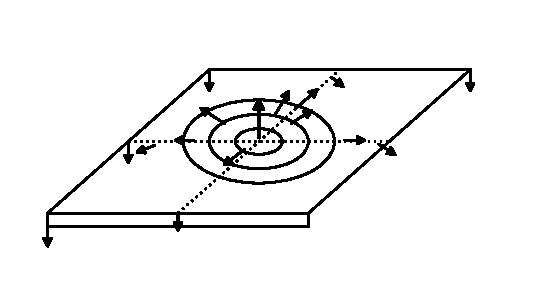
\includegraphics[width=0.72\textwidth]{fig_5.21.pdf}
\caption*{图 5.21\quad (1+1) 维 $O(3)$ 非线性 $\sigma$ 模型中的孤子/瞬子解。}
\end{figure}

为了回答这个问题，让我们考虑虚时并研究下面的 (1+1) 维系统：
\begin{equation*}
\frac{1}{2g}\left(|\partial_{\tau}\pmb{n}|^{2}+v^{2}|\partial_{\pmb{x}}\pmb{n}|^{2}\right)
\end{equation*}
上述作用量有一个非平凡的驻定"路径"，它是一个瞬子解（见图 5.21）。该作用量不依赖于瞬子的大小，其值为 $S_{0}=4\pi v/g$。这是因为，对任何 $\pmb{n}(x,\tau)$ 和任何标度因子 $b$，都有 $S(\pmb{n}(x,\tau))=S(\pmb{n}(bx,b\tau))$。

由于瞬子的作用量有限，瞬子的（时空）密度总是有限的。瞬子之间的平均间隔是 $l\,\mathrm{e}^{S_{0}/2}$ 的量级，其中 $l$ 是短距离截断。瞬子的大小也是 $l\,\mathrm{e}^{S_{0}/2}$ 的量级（因为瞬子的作用量不依赖于其大小）。这样，长程自旋序就被瞬子破坏了。自旋--自旋关联是短程的，关联长度为
\begin{equation*}
\xi=l\,\mathrm{e}^{S_{0}/2}=l\,\mathrm{e}^{2\pi v/g} \tag{5.6.8}
\end{equation*}
有趣的是，$\xi$ 或 $1/\xi$ 对 $g$ 是非微扰的。

我们看到，$O(3)$ 非线性 $\sigma$ 模型在 1+1 维具有短程关联，且所有激发都有能隙。然而，这个结果只对了一半。$O(3)$ 非线性 $\sigma$ 模型可以包含一个改变模型低能性质的拓扑项。

为了理解拓扑项的起源，让我们考虑 Hubbard 模型 (5.5.1) 的大 $U$ 极限。当 $U\gg t$ 时，Hubbard 模型（半填充时）的低能性质由海森堡模型描述：
\begin{equation*}
H=\sum_{\langle ij\rangle}J\,\pmb{S}_{i}\cdot\pmb{S}_{j} \tag{5.6.9}
\end{equation*}
其中 $\pmb{S}_{i}=c^{\dagger}_{i}\frac{\sigma}{2}c_{i}$ 是自旋算符，$J=4t^{2}/U$。海森堡模型的有效拉格朗日量为
\begin{equation*}
L=\mathrm{i}\sum_{i}z^{\dagger}_{i}\dot{z}_{i}-\frac{J}{4}\sum_{\langle ij\rangle}\pmb{n}_{i}\cdot\pmb{n}_{j} \tag{5.6.10}
\end{equation*}
其中 $z=\binom{z_{1}}{z_{2}}$，$\pmb{n}=z^{\dagger}\sigma z$。现在让我们假定海森堡模型的基态是反铁磁（AF）态 $\pmb{n}_{i}=(-)^{i}\hat{\pmb{z}}$，并且我们想研究 AF 基态附近的小涨落。

无能隙自旋波涨落由
\begin{equation*}
\pmb{n}_{i}(t)=(-)^{i}\pmb{n}(x^{i},t)
\end{equation*}
描述。人们很想把上式代入拉格朗日量 (5.6.10) 以得到一个连续的有效理论。然而，这种简单化的做法得不到正确的结果。一个原因是，所得拉格朗日量只含一阶时间导数项而不含二阶导数项。人们可以说，在低能下，一阶时间导数项比二阶时间导数项更重要，把二阶时间导数项丢掉应该没有问题。然而事实证明，一阶时间导数项是一个全导数，对运动方程没有影响。我们需要把二阶时间导数项包括进来，运动方程才具有非平庸的动力学。这里的情形与我们在 3.3.3 节遇到的情况非常相似，在那里我们从相互作用玻色模型导出了 XY 模型。

为了得到二阶时间导数项，我们考虑下面更一般的涨落：
\begin{equation*}
\pmb{n}_{i}(t)=(-)^{i}\pmb{n}(x^{i},t)+\pmb{m}(x^{i},t) \tag{5.6.11}
\end{equation*}
其中 $\pmb{n}(x,t)$ 是 $(x,t)$ 的光滑函数，满足 $|\pmb{n}(x,t)|=1$；$\pmb{m}(x,t)$ 也是 $(x,t)$ 的光滑函数，但 $|\pmb{m}(x,t)|\ll 1$，且 $\pmb{m}(x,t)\cdot\pmb{n}(x,t)=0$。这里 $\pmb{n}$ 描述低能的 AF 自旋波涨落，而 $\pmb{m}$ 描述能量很高、将被积掉的铁磁涨落。由于 $\int \mathrm{d}t\,2\mathrm{i}z^{\dagger}_{i}\dot{z}_{i}$ 是 $\pmb{n}_{i}$ 所张的立体角，我们有
\begin{equation*}
\int \mathrm{d}t\;2\mathrm{i}z^{\dagger}_{i}\dot{z}_{i}=\int \mathrm{d}t\;2\mathrm{i}(-)^{i}z(x^{i},t)^{\dagger}\dot{z}(x^{i},t)+\int \mathrm{d}t\;\pmb{n}\cdot(\dot{\pmb{n}}\times\pmb{m})
\end{equation*}
其中 $\pmb{n}(x,t)=z^{\dagger}(x,t)\sigma z(x,t)$，即
\begin{equation*}
\mathrm{i}\sum_{i}z^{\dagger}_{i}\dot{z}_{i}=\frac{1}{2}\int \mathrm{d}x\;\frac{1}{2}\,\pmb{n}\cdot(\partial_{t}\pmb{n}\times\partial_{x}\pmb{n})+\int \mathrm{d}x\;\frac{1}{2a}\,\pmb{n}\cdot(\dot{\pmb{n}}\times\pmb{m})
\end{equation*}
其中 $a$ 是晶格间距。$\frac{J}{4}\sum_{\langle ij\rangle}\pmb{n}_{i}\cdot\pmb{n}_{j}$ 项诱导出一个 $m^{2}$ 项。这样，积掉 $\pmb{m}$ 之后，我们得到
\begin{equation*}
S=\int \mathrm{d}t\,\mathrm{d}x\;\frac{1}{2g}\left[(\partial_{t}\pmb{n})^{2}-v^{2}(\partial_{x}\pmb{n})^{2}\right]+\theta W \tag{5.6.12}
\end{equation*}
其中 $\theta=\pi$。把它与我们之前算得的有效作用量，即式 (5.6.3)，相比较，上式多出了一项 $\theta W$：
\begin{equation*}
W=\int \mathrm{d}t\,\mathrm{d}x\;\frac{1}{4\pi}\,\pmb{n}\cdot(\partial_{t}\pmb{n}\times\partial_{x}\pmb{n}) \tag{5.6.13}
\end{equation*}
这样的项是一个拓扑项，因为对任何小变化 $\delta\pmb{n}$ 都有 $W(\pmb{n}+\delta\pmb{n})-W(\pmb{n})=0$。\footnote{我们注意到
\begin{equation*}
W(\pmb{n}+\delta\pmb{n})-W(\pmb{n})=\int \mathrm{d}t\,\mathrm{d}x\left[\frac{1}{4\pi}\,\pmb{n}\cdot(\partial_{t}\delta\pmb{n}\times\partial_{x}\pmb{n})+\frac{1}{4\pi}\,\pmb{n}\cdot(\partial_{t}\pmb{n}\times\partial_{x}\delta\pmb{n})\right]
\end{equation*}
因为 $\pmb{n}\cdot\delta\pmb{n}=0$，且 $\partial_{t}\pmb{n}\times\partial_{x}\pmb{n}$ 平行于 $\pmb{n}$。另外，
\begin{align*}
\int \mathrm{d}t\,\mathrm{d}x\;\pmb{n}\cdot(\partial_{t}\delta\pmb{n}\times\partial_{x}\pmb{n})&=\int \mathrm{d}t\,\mathrm{d}x\;\partial_{t}\delta\pmb{n}\cdot(\partial_{x}\pmb{n}\times\pmb{n})\\
&=-\int \mathrm{d}t\,\mathrm{d}x\left[\delta\pmb{n}\cdot(\partial_{t}\partial_{x}\pmb{n}\times\pmb{n})+\delta\pmb{n}\cdot(\partial_{x}\pmb{n}\times\partial_{t}\pmb{n})\right]\\
&=-\int \mathrm{d}t\,\mathrm{d}x\;\delta\pmb{n}\cdot(\partial_{t}\partial_{x}\pmb{n}\times\pmb{n}),
\end{align*}
类似地，
\begin{equation*}
\int \mathrm{d}t\,\mathrm{d}x\;\pmb{n}\cdot(\partial_{t}\pmb{n}\times\partial_{x}\delta\pmb{n})=+\int \mathrm{d}t\,\mathrm{d}x\;\delta\pmb{n}\cdot(\partial_{t}\partial_{x}\pmb{n}\times\pmb{n}).
\end{equation*}} 因此，对能够连续变形到彼此的不同 $\pmb{n}$，$W(\pmb{n})$ 取相同的值。注意，$\pmb{n}$ 是从二维平面 $\mathcal{R}^{2}$ 到球面 $S^{2}$ 的一个映射，即 $\mathcal{R}^{2}\to S^{2}$。这个映射确实有不同的类，各类之间不能连续变形到彼此。这些不同的类由一个缠绕数——$\mathcal{R}^{2}$ 缠绕 $S^{2}$ 的次数——来表征。式 (5.6.13) 中的 $W(\pmb{n})$ 只取整数值，正是缠绕数的一个数学表述。

与 $g$ 和 $v$ 不同，式 (5.6.12) 中 $\theta=\pi$ 的值是精确且量子化的。它不接收微扰展开中高阶项的修正。为看清这一点，我们注意到，平移一个晶格间距在我们的有效理论 (5.6.12) 中诱导变换 $\pmb{n}\to-\pmb{n}$。在这样的变换下，$S$ 应当不变。由于在该变换下 $W\to -W$，只有 $\theta=0$ 和 $\pi$ 与平移一个晶格间距的对称性相容。这样，只要底层晶格哈密顿量具有平移一个晶格间距的对称性，$\theta$ 就只能取 0 和 $\pi$ 两个值。由于 $\theta$ 的量子化，式 (5.6.12) 不仅适用于海森堡模型 (5.6.9)，也适用于 Hubbard 模型 (5.5.1) 的 AF 态。我们还注意到，对自旋为 $S$ 的海森堡模型，其 AF 态同样由 $O(3)$ 非线性 $\sigma$ 模型描述，只是现在 $\theta=2\pi S$。（如果我们显式破坏这一对称性，比如说令 $J_{i,i+1}\neq J_{i+1,i+2}$，则 $\theta$ 的值便不再量子化。）

上面关于瞬子把代数长程序变成短程序的讨论，只在 $\theta=0\ \mathrm{mod}\ 2\pi$ 时有效。因此，整数自旋的海森堡模型具有短程关联和有限能隙，其基态是自旋单态（对偶数格点的链）。对半整数自旋的海森堡模型，$\theta=\pi$，上述瞬子讨论不再有效。事实上，这种情形下自旋--自旋关联具有代数长程序，即 $\langle\pmb{S}_{i}\cdot\pmb{S}_{j}\rangle\sim 1/|i-j|$。基态仍是自旋单态（对偶数格点的链），但现在存在无能隙激发。

缠绕数还给出瞬子作用量 $S_{0}$ 的一个下界，即 $S_{0}\geqslant 4\pi v|W|/g$。\footnote{假定 $v=1$。对于 $\delta\tau=\delta x$ 的小正方形 $\delta\tau\times\delta x$，我们有
\begin{align*}
\int_{\delta\tau\times\delta x}\mathrm{d}\tau\,\mathrm{d}x\,\left[(\partial_{\tau}\pmb{n})^{2}+(\partial_{x}\pmb{n})^{2}\right]&=(\partial_{\tau}\pmb{n})^{2}+(\partial_{x}\pmb{n})^{2}\\
&\geqslant 2\,|\pmb{n}\cdot(\partial_{\tau}\pmb{n}\times\partial_{x}\pmb{n})|=2\left|\int_{\delta\tau\times\delta x}\mathrm{d}\tau\,\mathrm{d}x\;\pmb{n}\cdot(\partial_{\tau}\pmb{n}\times\partial_{x}\pmb{n})\right|.
\end{align*}
由缠绕数 $(4\pi)^{-1}\int \mathrm{d}\tau\,\mathrm{d}x\;\pmb{n}\cdot(\partial_{\tau}\pmb{n}\times\partial_{x}\pmb{n})=\pm 1$ 可得 $S_{0}\geqslant 4\pi v|W|/g$（我们已把 $v$ 放了回来）。} 事实上，瞬子解饱和该下界，$S_{0}=4\pi v/g$。

\subsection{量子数与低能激发}

\begin{keypoints}
\item 从连续的非线性 $\sigma$ 模型计算低能激发的晶体动量。
\end{keypoints}

让我们假定 $d>1$，且系统具有真正的长程 AF 序。AF 基态之上的低能激发由 $O(3)$ 非线性 $\sigma$ 模型描述：
\begin{equation*}
S=\int \mathrm{d}t\,\mathrm{d}x\;\frac{1}{2g}\left[(\partial_{t}\pmb{n})^{2}-v^{2}(\partial_{x}\pmb{n})^{2}\right] \tag{5.6.14}
\end{equation*}
这里我们想用 $S$ 计算有限系统的低能激发。

首先，让我们考虑均匀涨落，即
\begin{equation*}
\pmb{n}(\pmb{x},t)=\pmb{n}_{0}(t) \tag{5.6.15}
\end{equation*}
我们已经假定晶格在每个方向都有偶数个格点，因此上述拟设 (5.6.15) 可以与 AF 序相容。$\pmb{n}_{0}$ 的有效作用量为
\begin{equation*}
S_{0}=\int \mathrm{d}t\;\frac{M}{2}\dot{\pmb{n}}^{2}_{0}
\end{equation*}
其中 $M=\mathcal{V}/g$，$\mathcal{V}$ 是空间的体积。这里 $S_{0}$ 描述一个质量为 $M$ 的粒子在单位球面上的运动。能级由"角动量"标记，它就是我们系统中的总自旋 $(S,S_{z})$：$E_{S,S_{z}}=\frac{S(S+1)}{2M}$，$S_{z}=-S,-S+1,\ldots,S$。由于晶格有偶数个格点，$S$ 总是整数。我们注意到，$E_{S,S_{z}}$ 按 $\mathcal{V}^{-1}$ 标度，远低于最低自旋波激发的能量——后者在 $d>1$ 时按 $\mathcal{V}^{-1/d}$ 标度。

现在让我们考虑激发态 $|S,S_{z}\rangle$ 的动量。朴素地想，人们预期所有 $|S,S_{z}\rangle$ 态都携带零动量，因为它们来自常数 $\pmb{n}_{0}$。然而，$\pmb{n}_{0}$ 只在把偶（奇）格点变到偶（奇）格点的那些平移下不变。因此，$|S,S_{z}\rangle$ 只在这些平移下不变。这把 $|S,S_{z}\rangle$ 的动量限制为 0 或 $\pmb{Q}=(\pi,\pi,\ldots,\pi)$。在平移一个晶格间距时，$\pmb{n}_{0}\to -\pmb{n}_{0}$。于是，在 $\pmb{n}_{0}\to -\pmb{n}_{0}$ 下为偶的态携带零动量，而在 $\pmb{n}_{0}\to -\pmb{n}_{0}$ 下为奇的态携带动量 $\pmb{Q}$。我们发现，偶 $S$ 态携带零动量，奇 $S$ 态携带动量 $\pmb{Q}$。

\subsection*{问题 5.6.2}

从式 (5.6.10) 出发计算式 (5.6.12) 中的作用量 $S$（即由 $J$ 和晶格间距 $a$ 确定 $g$ 与 $v$ 的值）。

% ---------------------------------------------------------------------------
% 块边界备注（装配说明，非译文）：
% 1. 起点：书页 239（p254）顶部 "This allows us to calculate" 是书页 238（p253）
%    段落（"…we find that, in real space，[实空间关系式]"）的延续。本文件第 2 行为
%    %JOIN%，第 3 行起即续文"这使我们能够计算"，与 ch5_d 文件尾装配备注的请求一致；
%    本块不设 %--E-TAIL-- 区（无上一块收尾内容需要另写）。
% 2. 终点：本块为第 5 章章末块。书页 249（p264）以问题 5.6.2 收束，其后即为第 6 章
%    章首（p265），本块自然收尾，无 TAIL、无跨页半句。
% 3. 蓝本问题备注：
%    a) 蓝本式 (5.6.1) 处残留 "tag{5}+tag{5.6.1}" 双重编号，已按 PNG 归为单 tag；
%    b) 脚注 38 的第二个公式（"⩾2|n·(∂_τn×∂_x n)|=…"）被 MinerU 错插到 5.6.3 节
%       式 (5.6.14) 之后的正文位置，本块已按 PNG 归位入脚注 38；
%    c) 式 (5.5.6) 首行蓝本作 (u_k^2−v_k^2)，经放大核对与 PNG 一致（低分辨率整页
%       判读易误作 v_k^2−u_k^2，以放大图为准）；
%    d) 蓝本 5.6 节要点行前的 "\-" 系节首要点列表，已转 keypoints 环境；
%       式 (5.6.6)/(5.6.7) 的编号在原书中挂于三行公式的中间行，本块 align* 的
%       \tag 位置照此排。
% 4. 术语：能隙方程、约化布里渊区与 ch5_d 用法一致；SDW、RPA 沿用本章前文译名，
%    不再括注；新增术语已追加至术语表"第5章（ch5_e）"一节。

 % 本文件由 scripts/assemble.py 自动装配，勿手改（改 parts/ 后重跑）
% 第6章 量子规范理论

% 第6章 QUANTUM GAUGE THEORIES
% 块界说明：本块自章首起，至书页 262（p277）末段"……我们就求解了环面上的紧致 U(1) 规范理论。"自然结束；
% 书页 263（p278）顶部为新段落"接下来让我们转向 XY 模型……"，属下一块（ch6_b），无 TAIL/JOIN。
\chapter{量子规范理论}

量子场论大致可以分为三类，即玻色理论、费米理论和规范理论。玻色子与费米子的量子场论已在前几章中讨论过。本章我们将讨论规范理论。这里我们形式地引入规范理论，更物理的讨论将在第 10 章给出。

人们或许会奇怪，为什么量子场论恰好有三类。自然界选择用哪些量子场论来描述它自身？按照 $U(1)\times SU(2)\times SU(3)$ 标准模型，自然界选择了费米理论和规范理论。因此，规范理论对高能粒子物理十分重要。可是，自然界为什么选择较为复杂的费米理论和规范理论，而跳过了较简单的玻色理论？第 10 章将对上述问题给出回答。结果表明，我们并不是非得引入费米理论和规范理论不可：它们可以作为一个局域玻色系统的有效理论演生出来。既然规范理论是演生（emergent）的，那么规范理论也出现在某些凝聚态系统中就不足为奇了。事实上，从凝聚态系统演生出来的规范理论，其种类可能比我们的真空所提供的还要多。\footnote{这一演生图像还引出一个有趣的问题：除了费米理论和规范理论之外，还会不会有新的量子场论从玻色模型中演生出来？}

\section{简单规范理论}

\subsection{规范“对称性”与规范“对称性”破缺}

\begin{keypoints}
\item 规范理论是指我们用多于一个标签来标记同一个量子态的理论。\footnote{规范理论的这一观念相当非常规，但却是正确的。关于规范理论历史发展的讨论，见 10.7.4 节。}
\item 规范“对称性”不是对称性，永远不会被破坏。
\end{keypoints}

当两个不同的量子态 $|a\rangle$ 和 $|b\rangle$（即 $\langle a|b\rangle = 0$）具有相同的性质时，我们说 $|a\rangle$ 与 $|b\rangle$ 之间存在一个对称性。如果我们用两个不同的标签“$a$”和“$b$”来标记同一个态，$|a\rangle = |b\rangle$，那么 $|a\rangle$ 和 $|b\rangle$ 显然具有（或者说“它”具有）相同的性质。这时我们说 $|a\rangle$ 与 $|b\rangle$ 之间存在规范“对称性”，而关于 $|a\rangle$ 和 $|b\rangle$ 的理论就是一个规范理论（至少形式上是）。由于 $|a\rangle$ 和 $|b\rangle$ 是同一个态，总是具有（或者说“它”具有）相同的性质，因此根据定义，规范“对称性”永远不会被破坏。

通常，当同一个“东西”具有相同的性质时，我们并不说存在对称性。因此，“规范对称性”和“规范对称性破缺”是理论物理中最容易引起误解的两个术语。下面我们将不再使用这两个令人困惑的术语。当我们用多个标签来标记同一个态时，我们将说存在一个规范结构（gauge structure）（而不是规范“对称性”）；当我们改变标记方案时，我们将说规范结构发生了改变（而不是规范“对称性”破缺）。

\subsection{无规范场的规范理论}

\begin{keypoints}
\item 规范变换、规范不变态与规范不变算符的概念。
\end{keypoints}

上面那个规范理论的简单例子（只含一个态）太简单了。因此本节我们将研究一个更复杂些的例子。考虑在一个一维周期势中运动的粒子：
\begin{gather*}
H = \frac{1}{2m}p^2 + V\cos(2\pi x/a)\\
\mathcal{H} = \{|x\rangle\}\tag{6.1.1}
\end{gather*}
其中 $\mathcal{H}$ 是系统中可能态的希尔伯特空间。这里我们强调，单凭哈密顿量并不能确定一个系统；确定系统的正是哈密顿量\emph{和}希尔伯特空间 $(H,\mathcal{H})$。

上述系统具有平移对称性：
\begin{equation*}
T_a^\dagger H T_a = H, \qquad T_a|x\rangle = |x+a\rangle
\end{equation*}
我们可以把这一对称性变成一个规范结构，从而定义一个规范理论。所得的规范理论为
\begin{gather*}
H = \frac{1}{2m}p^2 + V\cos(2\pi x/a)\\
\mathcal{H}_a = \{|\psi\rangle,\ T_a|\psi\rangle = |\psi\rangle\}\tag{6.1.2}
\end{gather*}
也就是说，我们在保持“同一个”哈密顿量的同时，通过修改希尔伯特空间来定义我们的规范理论。新的希尔伯特空间是对称变换下的不变子空间。由于哈密顿量具有该对称性，它只在该不变子空间内起作用。我们称变换 $T_a$ 为规范变换（gauge transformation），称新希尔伯特空间中的态为规范不变态。我们的这个规范理论描述的其实只是一个圆上的粒子。

利用这个“更复杂”的规范理论，可以讨论规范理论的许多概念。对于直线上的粒子，态 $|x\rangle$ 和 $|x+a\rangle$ 是具有相同性质的不同态，因此存在平移对称性。对于圆上的粒子，$|x\rangle$ 和 $|x+a\rangle$ 是同一个态：这里 $x$ 和 $x+a$ 只是标记同一个量子态的两个标签。规范变换不过是标记同一个态的那些标签之间的变换。因此，根据定义，规范变换是一个“什么也不做”的变换；根据定义，所有物理态都是规范不变的。如果一个态不是规范不变的（即在我们的例子中，一个非周期的波函数 $\psi(x)$），那么这样的态不属于物理希尔伯特空间（即它不能是圆上粒子的波函数）。所有物理算符也必须是规范不变的，即 $O = T_a^\dagger O T_a$；否则，该算符将把一个物理态映射成物理希尔伯特空间之外的非物理态。我们看到，在规范理论中保持规范不变性是至关重要的：只有规范不变的态和规范不变的算符才是有意义的。

另一个我们熟悉的规范理论是全同粒子系统（identical-particle system），在其中交换对称性被变成了规范结构。考虑下列两粒子系统：
\begin{gather*}
H = H(x^1) + H(x^2)\\
\mathcal{H} = \{|x^1, x^2\rangle\}
\end{gather*}
它具有交换对称性 $(x^1, x^2) \to (x^2, x^1)$。然而，它并不是一个全同粒子系统。如果我们把交换对称性变成规范结构（即通过缩减希尔伯特空间），那么新系统由
\begin{gather*}
H = H(x^1) + H(x^2)\\
\mathcal{H}_b = \{|x^1, x^2\rangle \mid |x^1, x^2\rangle = |x^2, x^1\rangle\}.
\end{gather*}
描述，这样的系统就是一个全同粒子系统。注意，全同粒子系统并不具有交换\emph{对称性}，因为 $|x^1, x^2\rangle$ 和 $|x^2, x^1\rangle$ 根本就是同一个态。与全同粒子相联系的所有特殊干涉现象都来自规范结构。

\section{$Z_2$ 格点规范理论}

在本节中，我们将研究带有规范场的最简单的规范理论——$Z_2$ 规范理论。$Z_2$ 规范理论是最简单的拓扑场论。它作为若干具有拓扑序的量子液体态的有效理论而出现，我们将在第 9 章和第 10 章中讨论这些态。因此，$Z_2$ 规范理论对理解这些量子液体态的物理性质十分重要。

\begin{figure}[H]
\centering
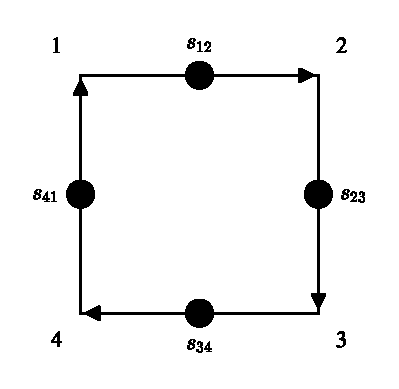
\includegraphics[width=0.72\textwidth]{fig_6.1.pdf}
\caption*{图 6.1\quad 一个正方形上的 $Z_2$ 规范理论。}
\end{figure}

正如任何量子理论一样，要定义一个 $Z_2$ 规范理论，我们需要定义它的希尔伯特空间和哈密顿量；要理解 $Z_2$ 规范理论的基本性质，我们需要求出它的激发谱。这就是我们在接下来几节中要做的事。

\subsection{希尔伯特空间}

\begin{keypoints}
\item $Z_2$ 规范理论中的态与位形的规范等价类之间存在一一对应。
\end{keypoints}

要定义一个量子的 $Z_2$ 格点规范理论（Wegner, 1971），我们首先需要定义它的希尔伯特空间。具体起见，让我们考虑一个用 $\pmb{i}$ 标记的二维正方格子。在每条最近邻链上，我们指定一个链变量 $s_{\pmb{ij}} = s_{\pmb{ji}}$，它可取 $\pm 1$ 两个值。希尔伯特空间中的态由 $s_{\pmb{ij}}$ 的位形标记，即 $|\{s_{\pmb{ij}}\}\rangle$。如果这种标记是一对一的，那么该希尔伯特空间就将是一个量子伊辛模型（自旋放在链上）的希尔伯特空间。为了得到 $Z_2$ 规范理论的希尔伯特空间，标记不是一对一的：两个规范等价的位形标记同一个量子态。

根据定义，如果两个位形 $s_{\pmb{ij}}$ 和 $\tilde{s}_{\pmb{ij}}$ 通过一个 $Z_2$ 规范变换
\begin{equation*}
\tilde{s}_{\pmb{ij}} = W_{\pmb{i}} s_{\pmb{ij}} W_{\pmb{j}}^{-1}\tag{6.2.1}
\end{equation*}
相联系，其中 $W_{\pmb{i}}$ 是取值 $\pm 1$ 的任意函数，则称它们规范等价。规范变换定义了一个等价关系。如果我们把所有相互规范等价的位形归成一组，这样的组就称为规范等价类。我们看到，希尔伯特空间中的态与规范等价类之间存在一一对应。

作为练习，让我们考虑一个正方形上的 $Z_2$ 规范理论（见图 6.1），求出其希尔伯特空间的维数。首先，有 4 条链，因此有 $2^4 = 16$ 个不同的 $s_{\pmb{ij}}$ 位形。其次，有 4 个格点，因此有 $2^4 = 16$ 个不同的 $Z_2$ 规范变换。如果一个规范等价类中位形的数目等于不同规范变换的数目，
\begin{figure}[H]
\centering
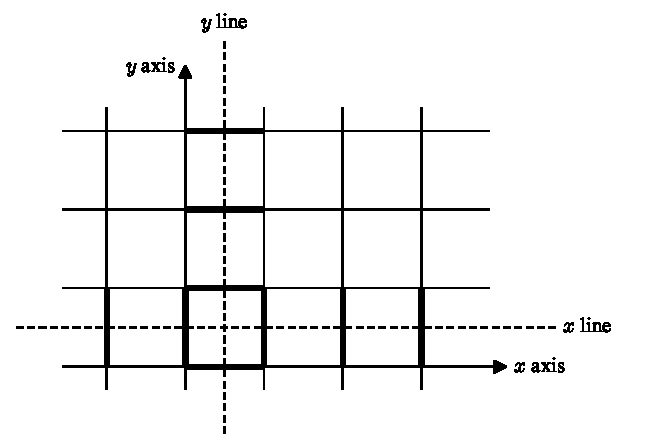
\includegraphics[width=0.72\textwidth]{fig_6.2.pdf}
\caption*{图 6.2\quad 跨过 $x$ 线和/或 $y$ 线的链可以再附加一个负号。}
\end{figure}
那么就将只有一个规范等价类。然而我们注意到，下面两个规范变换
\begin{equation*}
W_{\pmb{i}} = 1, \qquad W_{\pmb{i}} = -1
\end{equation*}
不改变位形 $s_{\pmb{ij}}$。这两个规范变换构成一个群，称为不变规范群（invariant gauge group，IGG）（另见 9.4.2 节）。于是，16 个规范变换只诱导出 $16/2 = 8$ 个规范等价的位形，因子 2 正是 IGG 中元素的数目。由于每个规范等价类含 8 个位形，故共有 $16/8 = 2$ 个规范等价类，从而希尔伯特空间中有两个态。

为了找到一种显式标记希尔伯特空间中各态的方法，重要的是找出在规范变换下不变的那些规范不变的量。其中一个规范不变的量是 Wegner--Wilson 圈变量（Wegner, 1971; Wilson, 1974），对一条回路 $C$ 定义为
\begin{equation*}
U(C) = s_{\pmb{ij}} s_{\pmb{jk}} \cdots s_{\pmb{li}}
\end{equation*}
其中 $\pmb{i}, \pmb{j}, \pmb{k}, \ldots, \pmb{l}$ 是回路上的格点。我们将称 $U(C)$ 为穿过该回路的 $Z_2$ 通量。读者容易验证：$U(C)$ 只取 $\pm 1$ 两个值，并且在 $Z_2$ 规范变换下不变。正方形上 $Z_2$ 规范理论的两个态由 $s_{12}s_{23}s_{34}s_{41} = \pm 1$ 标记。

现在我们来数一数有限正方格子上 $Z_2$ 规范理论中态的数目。设格子沿两个方向都有周期性边界条件（即格子构成一个环面）。若格子有 $N_{\text{site}}$ 个格点，则它有 $2N_{\text{site}}$ 条最近邻链，因而有 $2^{2N_{\text{site}}}$ 个不同的 $s_{\pmb{ij}}$ 位形。又有 $2^{N_{\text{site}}}$ 个不同的规范变换，而 IGG 仍有 2 个元素。于是共有 $\frac{2^{2N_{\text{site}}}}{2^{N_{\text{site}}}/2} = 2 \times 2^{N_{\text{site}}}$ 个不同的规范等价类，对应于 $2 \times 2^{N_{\text{site}}}$ 个不同的态。

为了找到标记这 $2 \times 2^{N_{\text{site}}}$ 个态的方法，我们考虑穿过一个方格（plaquette）的 $Z_2$ 通量：
\begin{equation*}
F_{\pmb{i}} = s_{\pmb{i},\pmb{i}+\pmb{x}} s_{\pmb{i}+\pmb{x},\pmb{i}+\pmb{x}+\pmb{y}} s_{\pmb{i}+\pmb{x}+\pmb{y},\pmb{i}+\pmb{y}} s_{\pmb{i}+\pmb{y},\pmb{i}}
\end{equation*}
由于共有 $N_{\text{site}}$ 个方格且 $F_{\pmb{i}} = \pm 1$，人们自然会以为不同的 $\{F_{\pmb{i}}\}$ 可以提供 $2^{N_{\text{site}}}$ 个不同的标记。然而，各 $F_{\pmb{i}}$ 并不独立，它们满足
\begin{equation*}
\prod_{\pmb{i}} F_{\pmb{i}} = 1\tag{6.2.2}
\end{equation*}
因此，$\{F_{\pmb{i}}\}$ 只能提供 $2^{N_{\text{site}}}/2$ 个不同的标记。显然，我们不能用 $\{F_{\pmb{i}}\}$ 标记全部 $2 \times 2^{N_{\text{site}}}$ 个态。事实上，每一个通量位形 $\{F_{\pmb{i}}\}$ 对应于四个不同的态。

为看清这一点，我们考虑由一个位形 $s^0_{\pmb{ij}}$ 得到的下列四个位形：
\begin{equation*}
s^{(m,n)}_{\pmb{ij}} = f_x^m(\pmb{ij}) f_y^n(\pmb{ij}) s^0_{\pmb{ij}}, \qquad m, n = 0, 1\tag{6.2.3}
\end{equation*}
函数 $f_{x,y}(\pmb{ij})$ 取 $-1$ 或 $1$：当链 $\pmb{ij}$ 跨过 $x$ 线时（见图 6.2）$f_x(\pmb{ij}) = -1$，否则 $f_x(\pmb{ij}) = 1$；类似地，当链 $\pmb{ij}$ 跨过 $y$ 线时 $f_y(\pmb{ij}) = -1$，否则 $f_y(\pmb{ij}) = 1$。这四个位形在每一个方格上给出相同的 $Z_2$ 通量 $F_{\pmb{i}}$。尽管如此，这四个位形并不规范等价（见问题 6.2.2），因为它们对应于从环面的两个洞插入不同的 $Z_2$ 通量（见图 9.6）。因此，$2^{N_{\text{site}}}/2$ 个不同的通量位形 $\{F_{\pmb{i}}\}$ 加上四重简并，使我们得以恢复 $2 \times 2^{N_{\text{site}}}$ 个态。

\subsection*{问题 6.2.1}

证明环面上的 $Z_2$ 规范理论满足式 (6.2.2)。

\subsection*{问题 6.2.2}

证明式 (6.2.3) 中的四个位形并不规范等价。（提示：考虑 $C$ 绕环面一整圈的 $U(C)$。）

\subsection*{问题 6.2.3}

$Z_2$ 规范理论的希尔伯特空间 $\mathcal{H}_{Z_2}$ 也可以从一个自旋-$1/2$ 模型的希尔伯特空间 $\mathcal{H}_{\text{spin}}$ 构造出来，该模型在正方格子的每条链上放有一个自旋。$\mathcal{H}_{\text{spin}}$ 有一个子空间 $\mathcal{H}_{\text{sub}}$，它由在所有形如 $\prod_{\langle\pmb{ij}\rangle} (\sigma^1_{\pmb{ij}})^{G_{\pmb{i}} - G_{\pmb{j}}}$ 的幺正变换下不变的态构成。这里 $G_{\pmb{i}}$ 是格点上的任意函数，取值 $G_{\pmb{i}} = 0, 1$；$\sigma^1_{\pmb{ij}}$ 是作用在链 $\langle \pmb{ij} \rangle$ 上的自旋上的自旋算符。证明 $\mathcal{H}_{\text{sub}} = \mathcal{H}_{Z_2}$，且 $\prod_{\langle\pmb{ij}\rangle} (\sigma^1_{\pmb{ij}})^{G_{\pmb{i}} - G_{\pmb{j}}}$ 生成 $Z_2$ 规范变换。

\subsection{哈密顿量}

\begin{keypoints}
\item $Z_2$ 规范理论的哈密顿量必须是规范不变的。
\end{keypoints}

到目前为止我们只讨论了 $Z_2$ 格点规范理论的希尔伯特空间。那么哈密顿量呢？我们不能随意挑一个 $Z_2$ 希尔伯特空间中的算符来充当哈密顿量。哈密顿量应当具有某些“局域”性质。构造局域哈密顿量的一种办法，是把它写成 $s_{\pmb{ij}}$ 的局域函数。然而，由于 $s_{\pmb{ij}}$ 是物理态的多对一标记，我们必须保证等价的标记给出相同的能量，也就是说，哈密顿量必须是规范不变的。构造规范不变哈密顿量的一个简单办法，是把哈密顿量写成规范不变算符（如 $U(C)$ 和 $F_{\pmb{i}}$）的函数。除了 $U(C)$ 之外，把一条链上的 $s_{\pmb{ij}}$ 变号的算符 $\sigma^1_{\pmb{ij}}$，即 $s_{\pmb{ij}} \to -s_{\pmb{ij}}$，也是规范不变算符（见问题 6.2.4）。于是，$Z_2$ 规范理论的一个规范不变的局域哈密顿量可以写成
\begin{equation*}
H_{Z_2} = -g \sum_{\pmb{i}} F_{\pmb{i}} - t \sum_{\langle \pmb{ij} \rangle} \sigma^1_{\pmb{ij}}\tag{6.2.4}
\end{equation*}

\subsection*{问题 6.2.4}

设 $\hat{W}$ 生成一个规范变换 $\hat{W}|\{s_{\pmb{ij}}\}\rangle = |\{\tilde{s}_{\pmb{ij}}\}\rangle$，其中 $\tilde{s}_{\pmb{ij}}$ 与 $s_{\pmb{ij}}$ 通过式 (6.2.1) 相联系。若算符 $\hat{O}$ 满足 $\hat{W}\hat{O}\hat{W}^{-1} = \hat{O}$，则称其为规范不变的。证明 $\sigma^1_{\pmb{ij}}$ 是规范不变算符。

\subsection{物理性质}

\begin{keypoints}
\item 尽管能隙有限，低能下的 $Z_2$ 规范理论并非平庸。它在环面上的低能性质由四重拓扑简并的基态表征。
\end{keypoints}

当 $t = 0$、$g > 0$ 时，$H_{Z_2}$ 在环面上有四个简并的基态，它们由 $F_{\pmb{i}} = +1$ 表征。激发通过翻转 $F_{\pmb{i}}$ 的符号产生（见图 6.3）。这些激发的行为像局域粒子，将被称为 $Z_2$ 涡旋。由于约束 (6.2.2)，在环面上 $Z_2$ 涡旋只能成对地产生。这些激发的能隙是 $g$ 的量级。$H_{Z_2}$ 中的 $t$ 项诱导 $Z_2$ 涡旋的跳跃。由于各 $\sigma^1_{\pmb{ij}}$ 算符彼此对易，利用跳跃算符的统计代数（见式 (4.1.10)），我们发现 $Z_2$ 涡旋是玻色子。

我们想指出，基态的四重简并是一种所谓的拓扑简并（topological degeneracy）。根据定义，拓扑简并是指不能被哈密顿量的任何局域微扰所消除的简并。拓扑简并十分重要，它使我们能够在第 8 章中定义拓扑序。

为了理解 $Z_2$ 规范理论中四重简并的稳健性，让我们把 $t$ 项当作微扰，看看 $t$ 项如何解除 $t = 0$ 哈密顿量的四重简并基态。四个简并的基态由 $s^0_{\pmb{ij}} = 1$ 时的式 (6.2.3) 给出。我们看到，把一个态 $s^{(m,n)}_{\pmb{ij}}$ 变成另一个不同的态 $s^{(m',n')}_{\pmb{ij}}$ 的唯一办法，是把 $s^0_{\pmb{ij}}$ 在环绕环面一整圈的一条链上的符号统统翻转。如果环面由 $L \times L$ 的格子构成，那么至少需要 $L$ 个 $\sigma^1_{\pmb{ij}}$ 算符才能连接不同的简并态，这只可能在微扰论的 $L$ 阶以上发生。因此，$t$ 项能够解除四重简并，但能量劈裂 $\Delta E$ 仅为 $t^L/g^{L-1}$ 的量级。在热力学极限下，$L \to \infty$，$\Delta E \to 0$。上述讨论不依赖于任何对称性，即使 $t$ 不均匀也成立。（热力学极限下的）四重简并是一个相的稳健性质。四重简并反映了 $Z_2$ 通量的低能动力学，是 $Z_2$ 规范理论最重要的特征。

\begin{figure}[H]
\centering
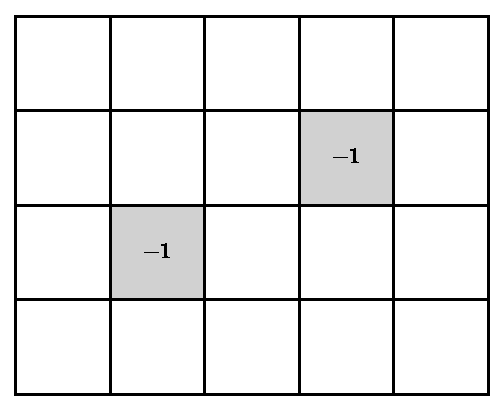
\includegraphics[width=0.72\textwidth]{fig_6.3.pdf}
\caption*{图 6.3\quad 把 $F_{\pmb{i}}$ 从 $+1$ 变到 $-1$ 产生一个 $Z_2$ 涡旋。}
\end{figure}

当 $g = 0$、$t > 0$ 时，$H_{Z_2}$ 的基态为
\begin{equation*}
|\Psi_0\rangle = \sum_{\{s_{\pmb{ij}}\}} |\{s_{\pmb{ij}}\}\rangle\tag{6.2.5}
\end{equation*}
其中求和 $\sum_{\{s_{\pmb{ij}}\}}$ 遍及所有位形 $\{s_{\pmb{ij}}\}$。该基态非简并，能量为 $-tN_l$，其中 $N_l$ 是链的数目。如果我们把 $H_{Z_2}$ 看作一个自旋放在链上的伊辛模型，这个结果很容易理解：这里 $s_{\pmb{ij}}$ 可以认定为自旋算符 $\sigma^3_{\pmb{ij}}$ 在 $z$ 方向的本征值，而 $\sigma^1_{\pmb{ij}}$ 是 $x$ 方向的自旋算符。在这一伊辛模型图像中，$|\Psi_0\rangle$ 态不过是所有自旋都指向 $x$ 方向的态。

从上述讨论我们看到，$H_{Z_2}$ 有两个相。当 $g \gg t$ 时，基态具有四重简并，激发是 $Z_2$ 涡旋。我们将称这个相为 $Z_2$ 解禁闭相（deconfined phase）。该相的低能性质由一个 $Z_2$ 规范理论描述。当 $g \ll t$ 时，基态不简并。我们将称这个相为 $Z_2$ 禁闭相（confined phase）。其低能性质不具有 $Z_2$ 规范理论的任何特征。

如果你觉得 $Z_2$ 规范理论的定义过于形式化，而且这样得到的 $Z_2$ 规范理论很古怪，那么你就抓住了要点。$Z_2$ 规范理论其实是一个非局域理论，其意义是：它的总希尔伯特空间不能表示成局域希尔伯特空间的直积。在 10.3 节中，我们将对 $Z_2$ 规范理论给出更物理的描述。我们将看到，$Z_2$ 规范理论其实是一种闭合弦的理论。

\begin{figure}[H]
\centering
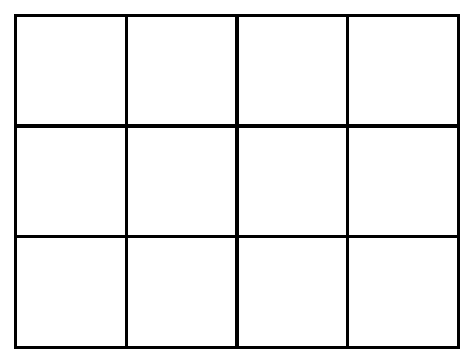
\includegraphics[width=0.72\textwidth]{fig_6.4.pdf}
\caption*{图 6.4\quad 一个开放的二维正方格子。}
\end{figure}

\subsection*{问题 6.2.5}

\begin{enumerate}
\item[(a)] 一个 $Z_2$ 规范理论 $H_{Z_2}$（见式 (6.2.4)）定义在一个 $L_x \times L_y$ 个格点的开放正方格子上（见图 6.4）。设 $t = 0$，求基态能量和简并度。
\item[(b)] 设格子沿 $y$ 方向周期，构成一个圆柱面。设 $t = 0$，求基态能量和简并度。
\item[(c)] 设格子沿 $x$、$y$ 两个方向都周期。设 $t = 0$ 且 $g < 0$，对下列三种情形求基态能量和简并度：(i) $L_x$ 为偶、$L_y$ 为偶；(ii) $L_x$ 为偶、$L_y$ 为奇；(iii) $L_x$ 为奇、$L_y$ 为奇。
\end{enumerate}

\subsection*{问题 6.2.6}

证明当 $g = 0$、$t > 0$ 时，式 (6.2.5) 是 $H_{Z_2}$ 的基态。

\subsection*{问题 6.2.7}

考虑 $L \times L$ 个格点的环面上的两个位形 $s^1_{\pmb{ij}}$ 和 $s^2_{\pmb{ij}}$。这两个位形生成相同的 $Z_2$ 通量 $F_{\pmb{i}}$。证明：如果这两个位形不规范等价，那么要把 $s^1_{\pmb{ij}}$ 变成 $s^2_{\pmb{ij}}$，至少需要翻转 $L$ 条链上 $s_{\pmb{ij}}$ 的符号（或者在多于 $L$ 条链上有 $s^1_{\pmb{ij}} s^2_{\pmb{ij}} = -1$）。

\subsection*{问题 6.2.8}

注意 $Z_2$ 涡旋的跳跃由跳跃算符 $P\sigma^1_{\pmb{ij}}P$、$P\sigma^1_{\pmb{ij}}P\sigma^1_{\pmb{jk}}P$ 等生成，其中 $P$ 是到具有固定 $Z_2$ 涡旋数的子空间上的投影。利用统计代数 (4.1.10)，证明 $Z_2$ 涡旋是玻色子。

\section{$1+2$ 维 $U(1)$ 规范理论与 XY 模型}

我们在 3.7.1 节构造了 $U(1)$ 规范理论的拉格朗日量，并在 3.7.5 节研究了它的经典运动方程。本节将研究量子的 $U(1)$ 规范理论。我们不是孤立地研究 $U(1)$ 规范理论，而是把它与 $1+2$ 维的 XY 模型放在一起研究。我们将证明，XY 模型与 $U(1)$ 规范理论之间存在对偶关系，并利用这一对偶关系研究 $(1+2)$ 维 $U(1)$ 规范理论中的瞬子效应与禁闭。

\subsection{$1+2$ 维 $U(1)$ 规范理论与 XY 模型之间的对偶}

\begin{keypoints}
\item 规范固定与库仑规范。
\item $U(1)$ 规范理论的量子化。
\item 量子化的电荷、大规范变换与紧致 $U(1)$ 规范理论。
\item $U(1)$ 规范理论中量子化的电荷就是对偶 XY 模型中量子化的涡旋。
\end{keypoints}

XY 模型由路径积分
\begin{gather*}
Z_{XY} = \int \mathcal{D}\theta\; \mathrm{e}^{\mathrm{i}\int \mathrm{d}t\,\mathrm{d}^2\pmb{x}\; \mathcal{L}_{XY}}\\
\mathcal{L}_{XY} = \frac{\chi}{2}\left(\dot{\theta}^{\,2} - (\partial_{\pmb{x}}\theta)^2\right)\tag{6.3.1}
\end{gather*}
描述。$U(1)$ 规范理论也可以由路径积分
\begin{gather*}
Z_{U(1)} = \int \mathcal{D}a_\mu\; \mathrm{e}^{\mathrm{i}\int \mathrm{d}t\,\mathrm{d}^2\pmb{x}\; \mathcal{L}_{U(1)}},\tag{6.3.2}\\
\mathcal{L}_{U(1)} = \frac{1}{2g^2}\left(\pmb{e}^2 - b^2\right), \qquad e_i = \partial_0 a_i - \partial_i a_0, \qquad b = \partial_1 a_2 - \partial_2 a_1,
\end{gather*}
描述，其中 $\pmb{e}$ 是 $a_\mu$ 的“电”场，$b$ 是它的“磁”场。这两条路径积分如此不同，以至于很难看出两个理论之间有任何关系。然而，我们下面将证明，这两条路径积分描述的是同一个物理系统。

我们注意到，两个理论都是二次的，因而都精确可解。理解两理论之间关系的一个办法，是把它们量子化，找出两个理论中所有的低能激发。

让我们先试着量子化 $U(1)$ 规范理论，即求出 $U(1)$ 规范理论的希尔伯特空间和哈密顿量。我们注意到，$\mathcal{L}_{U(1)}$ 在变换 $a_\mu \to a_\mu + \partial_\mu f$ 下不变：
\begin{equation*}
\mathcal{L}_{U(1)}(a_\mu) = \mathcal{L}_{U(1)}(a_\mu + \partial_\mu f)
\end{equation*}
如果我们把 $a_\mu$ 和 $a_\mu + \partial_\mu f$ 当作两条不同的路径，那么该理论就有一个对称性。然而在这里，我们把 $a_\mu$ 和 $a_\mu + \partial_\mu f$ 当作\emph{同一条}路径的两个不同标签。这样一来，我们得到的是一个规范理论，而 $a_\mu \to a_\mu + \partial_\mu f$ 定义了规范结构。

为了得到哈密顿量描述，我们先设法找到路径的一种一对一标记。考虑一条由 $a_\mu$ 标记的路径。规范变换告诉我们，$a'_\mu = a_\mu + \partial_\mu f$ 标记同一条路径。在同一条路径的这么多不同标签之中，通过调节 $f$，我们总可以挑选出满足
\begin{equation*}
\pmb{\partial} \cdot \pmb{a} = 0\tag{6.3.3}
\end{equation*}
的那一个。于是，满足式 (6.3.3) 的 $a_\mu$ 提供了不同路径的一种一对一标记。式 (6.3.3) 称为规范固定条件。能够导致路径一对一标记的规范固定条件有很多种；特定的规范固定条件 (6.3.3) 称为库仑规范。

在库仑规范中，作用量中含有 $a_0$ 的部分形如 $S = \int \mathrm{d}t\,\mathrm{d}^2\pmb{x}\; \pmb{e}^2 = \int \mathrm{d}t\,\mathrm{d}^2\pmb{x}\; (\dot{a}_i^2 + \partial_i a_0\, \partial_i a_0)$。交叉项 $\int \mathrm{d}t\,\mathrm{d}^2\pmb{x}\; \partial_i a_0\, \partial_0 a_i$ 因 $\partial_i a_i = 0$ 而消失。我们看到，$a_0$ 与 $\pmb{a}$ 解耦，且没有动力学（即没有 $\dot{a}_0$ 项）。因此我们可以丢掉 $a_0$（相当于取 $a_0 = 0$）。于是，在库仑规范中，路径积分计算的是从 $a_i(\pmb{x}, t_1)$ 到 $a_i(\pmb{x}, t_2)$、且满足 $\partial_i a_i(\pmb{x}, t) = 0$（$t_1 \leqslant t \leqslant t_2$）的演化的振幅。这样，$U(1)$ 规范理论的量子态由一个波泛函 $\Psi[a_i(\pmb{x})]$ 描述，其中 $a_i$ 满足 $\partial_i a_i = 0$。这就定义了物理态的希尔伯特空间。

接下来，我们将通过求出规范固定后的作用量来找出本征态及其能量。先把 $a_i$ 展开如下：
\begin{equation*}
a_i = \frac{X_i(t)}{L_i} + b_0 x^1 \delta_{i,2} + \sum_{\pmb{k}} \mathrm{i}\, c_{\pmb{k}}(t)\, \epsilon_{ij} k_j\, \mathrm{e}^{\mathrm{i}\pmb{k}\cdot\pmb{x}}\tag{6.3.4}
\end{equation*}
其中 $c_{\pmb{k}} = c^*_{-\pmb{k}}$。上式给出的 $a_i$ 总是满足 $\partial_i a_i = 0$。于是，物理态的波函数是 $b_0$、$X_i$ 和 $c_{\pmb{k}}$ 的函数。规范固定后的拉格朗日量形如
\begin{equation*}
L = \frac{1}{2g^2}\left(-b_0^2 L_1 L_2 + \frac{L_2}{L_1}\dot{X}_1^{\,2} + \frac{L_1}{L_2}\dot{X}_2^{\,2} + \sum_{\pmb{k}} \left(|\dot{c}_{\pmb{k}}|^2 - \pmb{k}^2 |c_{\pmb{k}}|^2\right) L_1 L_2 \pmb{k}^2\right)
\end{equation*}
我们看到，环面上的 $U(1)$ 规范理论由一集振子 $c_{\pmb{k}}$ 加上一个由 $(X_1, X_2)$ 描述的二维自由粒子所描述。本征态的能量为
\begin{equation*}
E = \frac{1}{2g^2} b_0^2 L_1 L_2 + \frac{g^2 L_1}{2L_2} P_1^2 + \frac{g^2 L_2}{2L_1} P_2^2 + \sum_{\pmb{k}} |\pmb{k}| n_{\pmb{k}}
\end{equation*}
其中 $n_{\pmb{k}}$ 是振子的占据数，$P_i$ 是与 $X_i$ 共轭的动量。

$U(1)$ 规范理论有两种，分别称为紧致与非紧致 $U(1)$ 理论（compact and non-compact $U(1)$ theories）。两种 $U(1)$ 规范理论中的规范变换定义不同，因此两个理论有不同的希尔伯特空间，应当加以区分。对于非紧致 $U(1)$ 理论，$a_\mu \to a_\mu + \partial_\mu f$ 是唯一允许的规范变换。我们后面会看到，在非紧致 $U(1)$ 理论中规范电荷不量子化。

紧致 $U(1)$ 规范理论具有量子化的规范电荷。只有 Wegner--Wilson 圈振幅
\begin{equation*}
O_C = \mathrm{e}^{-\mathrm{i} q \oint_C \mathrm{d}x^\mu a_\mu}
\end{equation*}
才可以被观测。这里 $q$ 是电荷量子。通过选取不同取向的小回路，可以证明 $O_C$ 包含电场 $\pmb{e}$ 和磁场 $b$ 的所有分量。由于 $O_C$ 是唯一的可观测量，任何使 $O_C$ 不变的 $a_\mu$ 的变换都是规范变换。这类变换具有 $a_\mu \to a_\mu + \partial_\mu f$ 的形式，但此时 $f$ 可以不是时空的单值函数。特别地，环面上的下列 $f$ 生成一个合法的规范变换：
\begin{equation*}
f = \frac{2\pi N_1 x^1}{q L_1} + \frac{2\pi N_2 x^2}{q L_2}\tag{6.3.5}
\end{equation*}
例如，对于沿 $x^1$ 方向环绕环面的回路 $C$，可以直接验证：在上述规范变换下，Wegner--Wilson 圈振幅按 $O_C \to O_C\, \mathrm{e}^{-\mathrm{i} q \oint_C \mathrm{d}x^\mu \partial_\mu f} = O_C$ 变换。

一般地，任何使 $\mathrm{e}^{\mathrm{i} q f}$ 单值的多值 $f$ 都使 $O_C$ 不变，这些 $f$ 生成合法的规范变换。我们还注意到，带电荷 $q$ 的电荷场按下式变换：
\begin{equation*}
\phi \to \mathrm{e}^{\mathrm{i} q f} \phi.
\end{equation*}
具有单值 $\mathrm{e}^{\mathrm{i} q f}$ 的规范变换保持电荷场单值。

式 (6.3.5) 中的规范变换称为大规范变换（large gauge transformations）。这些变换，即 $\mathrm{e}^{\mathrm{i} q f} = \exp\!\left(\mathrm{i}q\left(\frac{2\pi N_1 x^1}{qL_1} + \frac{2\pi N_2 x^2}{qL_2}\right)\right)$，不能连续变形为恒等变换 $\mathrm{e}^{\mathrm{i} q f} = 1$。当 $x^1$ 从 0 变到 $L_1$ 时，$\mathrm{e}^{\mathrm{i} q f}$ 在复平面的单位圆上绕行 $N_1$ 圈。缠绕数 $N_1$ 不能连续改变。

我们注意到，在规范变换 (6.3.5) 下，
\begin{equation*}
X_i \to X_i + 2\pi q^{-1} N_i
\end{equation*}
因此，对于紧致 $U(1)$ 理论，$(X_1, X_2)$、$(X_1 + 2\pi q^{-1}, X_2)$ 和 $(X_1, X_2 + 2\pi q^{-1})$ 标记同一个物理态（因为它们通过规范变换相联系）。由 $X_i$ 描述的自由粒子生活在大小为 $\frac{2\pi}{q} \times \frac{2\pi}{q}$ 的环面上。动量 $P_i$ 量子化为 $P_i = n_i q$。

对于非紧致 $U(1)$ 理论，不允许大规范变换。于是 $X_1$ 和 $X_2$ 没有周期条件，由 $X_i$ 描述的自由粒子生活在平面上。

我们看到，尽管两种理论的哈密顿量形式相同，紧致与非紧致 $U(1)$ 理论却有不同的物理希尔伯特空间。我们还看到，紧致 $U(1)$ 理论的 $q \to 0$ 极限给出非紧致 $U(1)$ 理论。这就是为什么我们说，在非紧致 $U(1)$ 理论中电荷是不量子化的。

\begin{figure}[H]
\centering
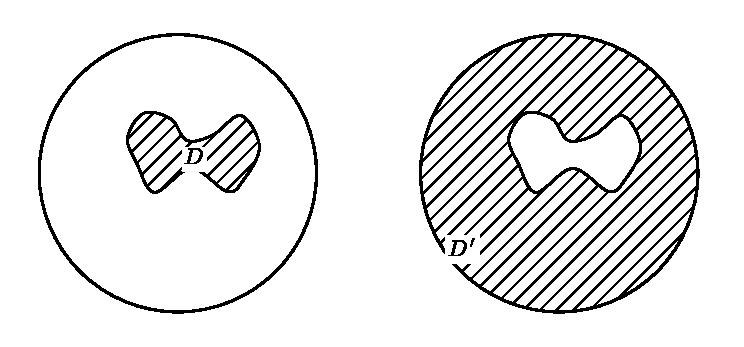
\includegraphics[width=0.72\textwidth]{fig_6.5.pdf}
\caption*{图 6.5\quad 单位球面上的一个圈可以是两个不同圆盘 $D$ 和 $D'$ 的边界。}
\end{figure}

由于我们的系统定义在环面上，每个物理量在 $x^1$ 和 $x^2$ 两个方向上都必须是周期的。人们也许会天真地把这一要求用于 $a_i$，要求 $a_i$ 是周期的：
\begin{equation*}
a_i(x^1, x^2) = a_i(x^1 + L_1, x^2) = a_i(x^1, x^2 + L_2).
\end{equation*}
然而我们注意到，$a_i$ 本身并不是物理的。不同的但规范等价的 $a_i$ 描述同一个物理态。因此，要使 $a_i$ 描述环面上的一个物理态，我们只要求 $a_i(x^1, x^2)$、$a_i(x^1 + L_1, x^2)$ 和 $a_i(x^1, x^2 + L_2)$ 规范等价。这只有当总磁通量子化时才可能发生（见问题 6.3.1）：
\begin{equation*}
\int \mathrm{d}^2\pmb{x}\; b = 2\pi N/q, \qquad N = \text{整数}\tag{6.3.6}
\end{equation*}
总通量的上述量子化，是圈振幅 $\mathrm{e}^{-\mathrm{i} q \int_C \mathrm{d}x^\mu a_\mu}$ 在紧致曲面上有意义所必需的。这是因为，对于二维空间 $S$ 中的回路 $C$，$\mathrm{e}^{-\mathrm{i} q \int_C \mathrm{d}x^\mu a_\mu} = \mathrm{e}^{\mathrm{i} q \int_D \mathrm{d}^2\pmb{x}\; b}$，其中 $D$ 是以回路 $C$ 为边界的二维圆盘。对于紧致二维空间，圆盘并不唯一（见图 6.5）。具有同一边界的两个不同圆盘 $D$ 和 $D'$ 相差紧致空间的总面积 $S$，故 $q\int_D \mathrm{d}^2\pmb{x}\; b - q\int_{D'} \mathrm{d}^2\pmb{x}\; b = q\int_S \mathrm{d}^2\pmb{x}\; b$。因此，为了让 $\mathrm{e}^{-\mathrm{i} q \int_C \mathrm{d}x^\mu a_\mu}$ 良好定义，$q\int_S \mathrm{d}^2\pmb{x}\; b/2\pi$ 必须量子化为整数。我们还注意到，对于非紧致 $U(1)$ 理论，$q = 0$，$\int_S \mathrm{d}^2\pmb{x}\; b$ 必须为零。

现在，紧致 $U(1)$ 规范理论的总能量可以改写为
\begin{equation*}
E = \frac{(2\pi)^2}{2g^2 q^2 L_1 L_2} N + \frac{g^2 q^2 L_1}{2L_2} n_1^2 + \frac{g^2 q^2 L_2}{2L_1} n_2^2 + \sum_{\pmb{k}} |\pmb{k}| n_{\pmb{k}}\tag{6.3.7}
\end{equation*}
环面上 $U(1)$ 规范理论的所有本征态都由一组整数 $(N, n_i, n_{\pmb{k}})$ 标记。这样，我们就求解了环面上的紧致 $U(1)$ 规范理论。

% ------------------------------------------------------------------
% 新增术语（ch6_a）
% ------------------------------------------------------------------
% gauge 'symmetry' / gauge 'symmetry' breaking : 规范“对称性” / 规范“对称性”破缺
% gauge-invariant states / operators : 规范不变态 / 规范不变算符
% gauge-equivalent class : 规范等价类
% invariant gauge group (IGG) : 不变规范群（IGG）
% Wegner–Wilson loop variable / amplitude : Wegner–Wilson 圈变量 / 圈振幅
% plaquette : 方格
% identical-particle system : 全同粒子系统
% exchange symmetry : 交换对称性
% translational symmetry : 平移对称性
% gauge-fixing condition : 规范固定条件
% large gauge transformation : 大规范变换
% compact / non-compact U(1) theory : 紧致 / 非紧致 U(1) 理论
% charge quantum : 电荷量子
% wave functional : 波泛函
% topological degeneracy : 拓扑简并
% Z2 vortex : Z2 涡旋
% deconfined / confined phase : 解禁闭相 / 禁闭相
% topological field theory : 拓扑场论
% energy splitting : 能量劈裂
% hopping operator : 跳跃算符
% quantum Ising model : 量子伊辛模型
% boson-number density / current density : 玻色子数密度 / 玻色子数流密度
% open lattice : 开放格子
% degeneracy : 简并度

% 块界说明：书页 262 以完整段落结束（"…we have solved the compact U(1) gauge theory on a torus."），
% 本块起始段为新段，无需 %JOIN%。本块为第 6 章章末块，至书页 274（p289）自然收束，无 TAIL。

下面我们转向 XY 模型及其本征态。我们展开
\begin{equation*}
\theta(t,\pmb{x})=\theta_{0}(t)+\frac{2\pi}{L_{i}}m_{i}x^{i}+\sum_{\pmb{k}}\lambda_{\pmb{k}}(t)\,\mathrm{e}^{\mathrm{i}\pmb{k}\cdot\pmb{x}}.
\end{equation*}
这里 $m_{1}$ 与 $m_{2}$ 分别是 $\theta$ 在 $x^{1}$ 与 $x^{2}$ 方向上的缠绕数。XY 模型的拉格朗日量现在具有如下形式：
\begin{equation*}
L=\frac{\chi}{2}\left(L_{1}L_{2}\dot{\theta}_{0}^{2}-\frac{(2\pi)^{2}L_{2}}{L_{1}}m_{1}^{2}-\frac{(2\pi)^{2}L_{1}}{L_{2}}m_{2}^{2}+L_{1}L_{2}\sum_{\pmb{k}}\left(|\dot{\lambda}_{\pmb{k}}|^{2}-\pmb{k}^{2}|\lambda_{\pmb{k}}|^{2}\right)\right)
\end{equation*}
我们看到，XY 模型由一群振子（由 $\lambda_{\pmb{k}}$ 描述）和一个圆上的自由粒子（由 $\theta_{0}$ 描述）构成。XY 模型的本征态由 $(N,m_{i},n_{\pmb{k}})$ 标记，其能量为
\begin{equation*}
E=\frac{1}{2\chi L_{1}L_{2}}N^{2}+\frac{\chi(2\pi)^{2}L_{2}}{2L_{1}}m_{1}^{2}+\frac{\chi(2\pi)^{2}L_{1}}{2L_{2}}m_{2}^{2}+\sum_{\pmb{k}}|\pmb{k}|n_{\pmb{k}} \tag{6.3.8}
\end{equation*}
我们看到，如果
\begin{equation*}
\chi=\left(\frac{qg}{2\pi}\right)^{2}
\end{equation*}
并且在标记 U(1) 理论与 XY 模型的本征态时把 $n_{i}$ 认作 $\epsilon_{ij}m_{j}$，那么 XY 模型与 U(1) 规范理论就具有完全相同的谱。本征态还携带确定的总动量 $\pmb{K}$：对 XY 模型的态 $|N,m_{i},n_{\pmb{k}}\rangle$ 或 U(1) 理论的态 $|N,n_{i},n_{\pmb{k}}\rangle$，
\begin{equation*}
K_{i}=Nm_{i}\frac{2\pi}{L_{i}}+\sum_{\pmb{k}}k_{i}n_{\pmb{k}}=N\epsilon_{ij}n_{j}\frac{2\pi}{L_{i}}+\sum_{\pmb{k}}k_{i}n_{\pmb{k}}.
\end{equation*}
从 XY 模型这一侧我们看到，标记 $N$ 具有物理意义：它是玻色子的总数减去平衡时的玻色子数，即 $N=N_{tot}-N_{0}$。因此，$\frac{1}{\chi}\dot{\theta}$ 与 $\frac{q}{2\pi}b$ 可以看作玻色子数密度减去平衡密度：
\begin{equation*}
\rho-\rho_{0}=\frac{q}{2\pi}b=\frac{1}{\chi}\dot{\theta}
\end{equation*}
U(1) 理论中的约束 $\partial_{0}b-\epsilon_{ij}\partial_{i}e_{j}=0$ 可以看作守恒流的连续性方程，即 $\partial_{0}\rho+\partial_{i}j_{i}=0$。于是，若把 $\frac{q}{2\pi}b$ 认作玻色子数密度，则 U(1) 理论中的玻色子数流密度由下式给出：
\begin{equation*}
j_{i}=-\frac{q}{2\pi}\epsilon_{ij}e_{j}
\end{equation*}

XY 模型的运动方程，即 $\partial_{0}^{2}\theta-\partial_{x}^{2}\theta=0$，同样可以看作守恒流的连续性方程。我们发现，在 XY 模型中同一个流由下式给出：
\begin{equation*}
j_{i}=-\frac{1}{\chi}\partial_{i}\theta
\end{equation*}
我们发现，U(1) 理论中的场与 XY 模型中的场之间存在一个简单关系：
\begin{equation*}
\frac{q}{2\pi}b=\frac{1}{\chi}\dot{\theta}, \qquad\qquad \frac{q}{2\pi}\epsilon_{ij}e_{j}=\frac{1}{\chi}\partial_{i}\theta. \tag{6.3.9}
\end{equation*}
事实上，把式 (6.3.9) 代入式 (6.3.2)，就会把 U(1) 规范拉格朗日量变成 XY 模型的拉格朗日量 (6.3.1)。这是看出 2+1 维中 U(1) 规范理论与 XY 模型之间对偶关系最直接的途径。

U(1) 规范理论可以与电荷耦合。设 $J_{\mu}$ 为 U(1) 电荷的密度与流密度，则耦合后的拉格朗日量具有如下形式：
\begin{equation*}
\mathcal{L}=\frac{1}{2g^{2}}(e^{2}-b^{2})-J_{\mu}a_{\mu}
\end{equation*}
对于位于 $\pmb{x}=0$ 处的点电荷，我们有 $J_{0}=q\delta(\pmb{x})$，并且从运动方程得到
\begin{equation*}
\frac{1}{g^{2}}\pmb{\partial}\cdot\pmb{e}=q\delta(\pmb{x})
\end{equation*}
即
\begin{equation*}
\pmb{e}=\frac{g^{2}q\pmb{x}}{2\pi\pmb{x}^{2}}
\end{equation*}
上面的 $\pmb{e}$ 对应于 XY 模型中的一个环形流：
\begin{equation*}
\partial_{i}\theta=\frac{\chi q}{2\pi}\frac{g^{2}q}{2\pi\pmb{x}^{2}}\epsilon_{ij}x^{j}=\frac{\epsilon_{ij}x^{j}}{\pmb{x}^{2}}
\end{equation*}
我们看到，U(1) 规范理论中的量子化电荷正是 XY 模型中的量子化涡旋。

\subsection*{问题 6.3.1}

证明式 (6.3.6)。（提示：你会发现展开式 (6.3.4) 很有用。）

\subsection*{问题 6.3.2}

将 1+1 维的紧致 U(1) 规范理论量子化，假设空间是长度为 $L$ 的一个圆环，电荷量子为 $q$。求标记所有能量本征态的整数集合，并求出这些本征态的能量。

\subsection{1+2 维紧致 U(1) 规范理论的禁闭}

\begin{keypoints}
\item 1+2 维 U(1) 规范理论中的瞬子效应赋予规范玻色子有限的能隙，并导致 U(1) 电荷之间的禁闭。
\item 瞬子效应可以用对偶 XY 模型中的一个 $\cos(\theta)$ 项来描述。
\end{keypoints}

这里我们考虑虚时间中的 U(1) 规范理论：
\begin{equation*}
\mathcal{L}_{U(1)}=\frac{1}{2g^{2}}\left(e^{2}+b^{2}\right) \tag{6.3.10}
\end{equation*}
形式上看，U(1) 规范理论像是一个具有无能隙激发的自由理论。然而事情并非如此简单。对于具有有限截断标度的紧致 U(1) 规范理论，理论中含有瞬子。瞬子效应将使 U(1) 规范理论成为一个相互作用理论。我们将会看到，这种相互作用会以剧烈的方式影响 U(1) 规范理论的低能性质。

什么是瞬子？位于 $x^{\mu}=0$ 处的瞬子由如下位形描述：
\begin{equation*}
b(x^{\mu})=\frac{1}{2q}\frac{x^{0}}{|\pmb{x}|^{3}}, \qquad e_{i}(x^{\mu})=\frac{1}{2q}\frac{x^{i}}{|\pmb{x}|^{3}}
\end{equation*}
上述瞬子的设计意图是使通量改变 $2\pi/q$，即
\begin{equation*}
\int_{x^{0}>0}\mathrm{d}^{2}x\,b-\int_{x^{0}<0}\mathrm{d}^{2}x\,b=\frac{2\pi}{q}
\end{equation*}
这是与电荷量子 $q$ 相容的最小允许瞬子。在存在有限截断时，路径积分不仅应当包含规范场的光滑涨落，还应当包含瞬子涨落。

把瞬子效应包括进来之后，U(1) 规范理论就不再是自由理论。现在的问题是如何理解含瞬子的紧致 U(1) 理论的低能性质。一种方法是利用 XY 模型与 U(1) 规范理论之间的对偶性。

对虚时间而言，$\theta$ 与 $a_{\mu}$ 通过下式相联系：
\begin{equation*}
\frac{q}{2\pi}b=\frac{1}{\chi}\dot{\theta}, \qquad \frac{q}{2\pi}\epsilon_{ij}e_{j}=-\frac{1}{\chi}\partial_{i}\theta \tag{6.3.11}
\end{equation*}
此式也可写为
\begin{equation*}
\frac{q}{2\pi}\epsilon_{\mu\nu\lambda}\partial_{\nu}a_{\lambda}=\frac{1}{\chi}\partial_{\mu}\theta \tag{6.3.12}
\end{equation*}
把式 (6.3.12) 代入式 (6.3.10) 后，我们得到
\begin{equation*}
\mathcal{L}=\frac{\chi}{2}(\partial_{\mu}\theta)^{2}
\end{equation*}
其中 $\chi=\left(\frac{qg}{2\pi}\right)^{2}$。我们注意到，瞬子产生 $2\pi/q$ 的通量。如前所见，这样一份通量对应于 XY 模型中的一个粒子。因此，瞬子产生或湮灭一个粒子。在 XY 模型中，产生或湮灭一个粒子的算符正是 $\mathrm{e}^{\pm\mathrm{i}\theta}$。我们发现，位于 $x^{\mu}$ 处的瞬子对应于 $\mathrm{e}^{\mathrm{i}\theta(x^{\mu})}$。由于瞬子与反瞬子在路径积分中以相同的权重出现，我们可以通过在 XY 模型中加入一项 $\mathrm{e}^{\mathrm{i}\theta}+\mathrm{e}^{-\mathrm{i}\theta}=2\cos(\theta)$ 来把瞬子效应包括进来，如下所示：
\begin{equation*}
\mathcal{L}=\frac{\chi}{2}(\partial_{\mu}\theta)^{2}-K\cos(\theta)
\end{equation*}

当 $\chi$ 很大时，$\theta$ 在 $\theta=0$ 附近的涨落很小。我们可以把 $\mathcal{L}$ 近似为
\begin{equation*}
\mathcal{L}=\frac{\chi}{2}(\partial_{\mu}\theta)^{2}+\frac{1}{2}K\theta^{2}
\end{equation*}

把瞬子效应包括进来之后，$\partial_{\mu}\theta$ 之间（或 $(b,e_{i})$ 之间）的关联变成短程的。我们看到，瞬子效应在 1+2 维中为 U(1) 规范场打开了能隙。这里我们想强调，$K\cos(\theta)$ 项是一个相关微扰，无论 $K$ 多么小，U(1) 规范玻色子都会获得能隙。

如果规范玻色子是无能隙的，那么在 1+2 维中带电粒子之间将通过对数势相互作用。电荷为 $q$ 的粒子与电荷为 $-q$ 的粒子之间的势由下式给出：
\begin{equation*}
\pi\frac{g^{2}q^{2}}{(2\pi)^{2}}\ln r=\pi\chi\ln r
\end{equation*}

把瞬子效应包括进来之后，规范场获得了能隙。但瞬子效应会如何影响带电粒子之间的长程相互作用呢？我们注意到，电荷为 $q$ 的粒子在 XY 模型中由一个涡旋描述。在瞬子效应存在时，即在 $K\cos(\theta)$ 项存在时，涡旋与反涡旋之间的势随两个涡旋的间距线性增长（见图 6.6）。因此，瞬子效应把对数势变成了电荷之间的线性势。

我们已经证明，在 1+2 维中 XY 模型可以用紧致 U(1) 规范理论来描述；我们也已经证明，U(1) 规范理论中的瞬子效应会打开能隙。这两个结果似乎相互矛盾：具有无能隙 Nambu--Goldstone 模的 XY 模型，怎么会等价于有能隙的 U(1) 规范理论呢？然而我们意识到，瞬子会产生通量，而通量对应于粒子数，所以瞬子的存在意味着相应 XY 模型中的粒子数不守恒。于是一切都自洽了。在瞬子存在时，粒子数不守恒。紧致 U(1) 规范理论描述的是一个不具有 U(1) 对称性的 XY 模型。这解释了为什么瞬子效应对应于 XY 模型中的势项 $K\cos(\theta)$。反过来，如果 XY 模型具有 U(1) 对称性并保持粒子数守恒，那么相应的 U(1) 规范理论中就不允许存在瞬子。

\begin{figure}[H]
\centering
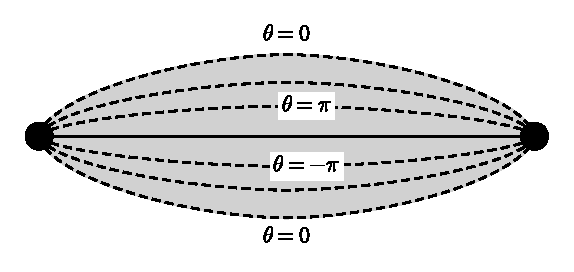
\includegraphics[width=0.72\textwidth]{fig_6.6.pdf}
\caption*{图 6.6\quad XY 模型中相距 $l$ 的涡旋--反涡旋对：$\theta$ 场在连接两个涡旋的连线的两侧必须跳变 $2\pi$。在 $-K\cos(\theta)$ 项存在时，通常的涡旋拟设 $\theta(x,y)=\arctan(x/y)$ 付出巨大的能量，其大小按 $l^{2}$ 增长。为使能量最小，非零的 $\theta$ 被限制在阴影区内。（虚线是 $\theta$ 场的等值线。）这导致两个涡旋之间的线性禁闭势。}
\end{figure}

\subsection*{问题 6.3.3}

\textbf{含瞬子的 1+2 维 U(1) 规范理论与含 $\cos(\theta)$ 项的 XY 模型之间的对偶性}

\begin{enumerate}
\item 计算在 $x^{\mu}$ 处有一个瞬子、在 $y^{\mu}$ 处有一个反瞬子的 U(1) 规范理论的配分函数 $Z(x^{\mu},y^{\mu})$，精确到一个整体常数因子。
\item 利用上述结果，写出包含多瞬子气体贡献的 U(1) 规范理论配分函数的表达式。
\item 计算在 $x^{\mu}$ 处插入 $\mathrm{e}^{\mathrm{i}\theta}$、在 $y^{\mu}$ 处插入 $\mathrm{e}^{-\mathrm{i}\theta}$ 的 XY 模型的下列配分函数 $Z(x^{\mu},y^{\mu})$，精确到一个整体常数因子：
\begin{equation*}
Z(x^{\mu},y^{\mu})=\int\mathcal{D}\theta\,\mathrm{e}^{\mathrm{i}\theta(x^{\mu})}\mathrm{e}^{-\mathrm{i}\theta(y^{\mu})}\mathrm{e}^{-\int\mathrm{d}^{3}x^{\mu}\,\mathcal{L}_{XY}(\theta)}
\end{equation*}
\item 证明：含瞬子的 U(1) 配分函数与加了 $K\cos(\theta)$ 项的 XY 模型配分函数相一致（按 $K$ 的幂次展开之后）。
\end{enumerate}

\section{格点上的量子 U(1) 规范理论}

\subsection{格点 U(1) 规范理论的拉格朗日量}

\begin{keypoints}
\item 格点 U(1) 规范理论由链上的变量 $a_{\pmb{i}\pmb{j}}$ 与格点上的变量 $a_{0}(\pmb{i})$ 描述。
\item 紧致与非紧致的格点 U(1) 规范理论。
\item 电场 $e_{\pmb{i}\pmb{j}}$ 的通量。
\end{keypoints}

U(1) 规范理论也可以定义在格点上。U(1) 格点规范理论使我们能够在任意维度中研究强耦合极限与禁闭。为简单起见，这里我们考虑二维正方格子上的 U(1) 规范理论。标势 $a_{0}(\pmb{x})$ 定义在每个格点 $\pmb{i}$ 上，记作 $a_{0}(\pmb{i})$；矢势 $\pmb{a}(\pmb{x})$ 定义在每条链上，记作 $a_{\pmb{i}\pmb{j}}$。我们注意到，$a_{\pmb{i}\pmb{j}}$ 与 $a_{\pmb{j}\pmb{i}}$ 并不独立，它们通过 $a_{\pmb{i}\pmb{j}}=-a_{\pmb{j}\pmb{i}}$ 相联系。连续场与格点场通过下式相联系：
\begin{equation*}
a_{0}(\pmb{j})=a_{0}(\pmb{x})|_{\pmb{x}=l\pmb{j}}, \qquad a_{\pmb{j}_{1}\pmb{j}_{2}}=\int_{l\pmb{j}_{1}}^{l\pmb{j}_{2}}\mathrm{d}x^{i}a_{i}(\pmb{x}) \tag{6.4.1}
\end{equation*}
其中 $l$ 是晶格常数。描述 U(1) 格点规范理论的拉格朗日量是 $a_{0}(\pmb{i})$ 与 $a_{\pmb{i}\pmb{j}}$ 的下列函数：
\begin{equation*}
L=\frac{1}{4J}\sum_{\pmb{i},\pmb{\mu}=\pmb{x},\pmb{y}}\left[\dot{a}_{\pmb{i},\pmb{i}+\pmb{\mu}}+a_{0}(\pmb{i})-a_{0}(\pmb{i}+\pmb{\mu})\right]^{2}-\frac{g}{2}\sum_{\pmb{p}}\Phi_{\pmb{p}}^{2} \tag{6.4.2}
\end{equation*}
其中 $\Phi_{\pmb{p}}$ 是穿过标记为 $\pmb{p}$ 的正方形的 U(1) 通量：
\begin{equation*}
\Phi_{\pmb{p}}=a_{\pmb{i},\pmb{i}+\pmb{x}}+a_{\pmb{i}+\pmb{x},\pmb{i}+\pmb{x}+\pmb{y}}+a_{\pmb{i}+\pmb{x}+\pmb{y},\pmb{i}+\pmb{y}}+a_{\pmb{i}+\pmb{y},\pmb{i}}. \tag{6.4.3}
\end{equation*}
可以直接验证，上述拉格朗日量在下列格点 U(1) 规范变换
\begin{equation*}
a_{\pmb{i}\pmb{j}}(t)\rightarrow a_{\pmb{i}\pmb{j}}(t)+\phi_{\pmb{j}}(t)-\phi_{\pmb{i}}(t), \qquad a_{0}(\pmb{i},t)\rightarrow a_{0}(\pmb{i},t)+\dot{\phi}_{\pmb{i}}(t) \tag{6.4.4}
\end{equation*}
之下不变。

式 (6.4.2) 定义的是一个非紧致的格点 U(1) 规范理论。紧致的格点 U(1) 规范理论则通过把 $u_{\pmb{i}\pmb{j}}=\mathrm{e}^{\mathrm{i}a_{\pmb{i}\pmb{j}}}$ 取作链变量来定义。在紧致格点 U(1) 规范理论中，$a_{\pmb{i}\pmb{j}}$ 与 $a'_{\pmb{i}\pmb{j}}=a_{\pmb{i}\pmb{j}}+2\pi$ 被视为等价。紧致格点 U(1) 规范理论的拉格朗日量具有如下形式：
\begin{equation*}
L=\frac{1}{4J}\sum_{\pmb{i},\pmb{\mu}=\pmb{x},\pmb{y}}\left[\dot{a}_{\pmb{i},\pmb{i}+\pmb{\mu}}+a_{0}(\pmb{i})-a_{0}(\pmb{i}+\pmb{\mu})\right]^{2}+g\sum_{\pmb{p}}\cos(\Phi_{\pmb{p}}) \tag{6.4.5}
\end{equation*}
它由式 (6.4.2) 修改而来，以便与周期性条件 $a_{\pmb{i}\pmb{j}}\sim a_{\pmb{i}\pmb{j}}+2\pi$ 相容。在本节余下的部分中，我们只考虑紧致 U(1) 格点规范理论。

经典运动方程由 $\delta L/\delta a_{\pmb{i}\pmb{j}}=0$ 与 $\delta L/\delta a_{0}(\pmb{i})=0$ 得到。我们发现
\begin{equation*}
\frac{1}{2J}\frac{\mathrm{d}e_{\pmb{i},\pmb{i}+\pmb{\mu}}}{\mathrm{d}t}+g\left[\sin(\Phi_{\pmb{p}_{1}})-\sin(\Phi_{\pmb{p}_{2}})\right]=0, \tag{6.4.6}
\end{equation*}
\begin{equation*}
\sum_{\pmb{\mu}=\pm\pmb{x},\pm\pmb{y}}e_{\pmb{i},\pmb{i}+\pmb{\mu}}=0, \qquad e_{\pmb{i}\pmb{j}}=\dot{a}_{\pmb{i}\pmb{j}}+a_{0}(\pmb{i})-a_{0}(\pmb{j}) \tag{6.4.7}
\end{equation*}
其中 $\pmb{p}_{1}$ 与 $\pmb{p}_{2}$ 标记链 $(\pmb{i},\pmb{i}+\pmb{\mu})$ 两侧的两个正方形。

把 $e_{\pmb{i}\pmb{j}}$ 与连续模型中的 $e$ 作比较，我们看到 $e_{\pmb{i}\pmb{j}}$ 可以解释为流过链 $(\pmb{i},\pmb{j})$ 的电场通量。式 (6.4.7) 表明电通量是守恒的，它对应于连续模型中的高斯定律 $\pmb{\partial}_{\pmb{x}}\cdot\pmb{e}=0$。此外，$\Phi_{\pmb{p}}$ 作为穿过正方形 $S_{\pmb{p}}$ 的通量，对应于连续模型中的 $\Phi_{\pmb{p}}=\int_{S_{\pmb{p}}}\mathrm{d}^{2}\pmb{x}\,b$。

要获得式 (6.4.2) 或式 (6.4.5) 所描述的格点 U(1) 规范理论的动力学性质，最简单的办法是取连续极限。假设 $a_{\mu}$ 很小并且是 $t$ 与 $\pmb{x}$ 的光滑函数，我们把连续变量与格点变量之间的关系式 (6.4.1) 代入格点拉格朗日量，便得到下列标准的 U(1) 拉格朗日量：
\begin{equation*}
\mathcal{L}=\frac{1}{8\pi\alpha_{2D}}\left(\frac{1}{c}e^{2}-cb^{2}\right) \tag{6.4.8}
\end{equation*}
从所得的麦克斯韦方程我们发现，格点 U(1) 规范理论含有一个速度为 $c$ 的无能隙模式。耦合常数 $\alpha_{2D}$ 在 1+2 维中的量纲为 1/长度。

在 3.7.1 节中，我们曾利用规范不变性在连续空间中构造了带电玻色子与 U(1) 规范场相耦合的理论。同样的构造也适用于格点模型。我们发现，与带电玻色子耦合的格点 U(1) 规范理论由下列拉格朗日量描述：
\begin{align*}
L={}&+\sum_{\langle\pmb{i}\pmb{j}\rangle}t_{\pmb{i}\pmb{j}}\left(\varphi_{\pmb{i}}^{\dagger}\varphi_{\pmb{j}}\mathrm{e}^{-\mathrm{i}a_{\pmb{j}\pmb{i}}}+h.c\right)+\sum_{\pmb{i}}\varphi_{\pmb{i}}^{\dagger}\,\mathrm{i}\left[\partial_{0}+\mathrm{i}a_{0}(\pmb{i})\right]\varphi_{\pmb{i}}\\
&+\frac{1}{4J}\sum_{\pmb{i},\pmb{\mu}=\pmb{x},\pmb{y}}\left[\dot{a}_{\pmb{i},\pmb{i}+\pmb{\mu}}+a_{0}(\pmb{i})-a_{0}(\pmb{i}+\pmb{\mu})\right]^{2}+g\sum_{\pmb{p}}\cos(\Phi_{\pmb{p}}) \tag{6.4.9}
\end{align*}
该拉格朗日量在下列格点规范变换下不变：
\begin{equation*}
c_{\pmb{i}}\rightarrow\mathrm{e}^{\mathrm{i}\phi(\pmb{i},t)}c_{\pmb{i}}, \quad a_{0}(\pmb{i})\rightarrow a_{0}(\pmb{i})-\partial_{0}\phi(\pmb{i},t), \quad a_{\pmb{i}\pmb{j}}\rightarrow a_{\pmb{i}\pmb{j}}+\phi(\pmb{i},t)-\phi(\pmb{j},t).
\end{equation*}

\subsection*{问题 6.4.1}

\begin{enumerate}
\item[(a)] 把式 (6.4.1) 推广到三维立方格子。
\item[(b)] 利用式 (6.4.1) 证明，三维格点规范理论的拉格朗日量在连续极限下变为 $\frac{1}{8\pi\alpha}(c^{-1}\pmb{e}^{2}-c\pmb{b}^{2})$，其中 $e_{i}=\partial_{0}a_{i}-\partial_{i}a_{0}$，$b_{i}=\epsilon_{ijk}\partial_{j}a_{k}$。试用 $J$、$g$ 与晶格常数 $l$ 求出 $\alpha$ 和 $c$ 的值。这里无量纲常数 $\alpha$ 就是精细结构常数，$c$ 是光速。
\end{enumerate}

\begin{figure}[H]
\centering
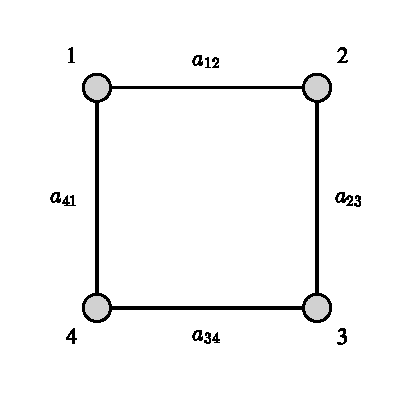
\includegraphics[width=0.72\textwidth]{fig_6.7.pdf}
\caption*{图 6.7\quad 一个正方形上的 U(1) 规范理论。}
\end{figure}

\subsection{格点 U(1) 规范理论的哈密顿量}

\begin{keypoints}
\item 格点 U(1) 规范理论的哈密顿量可以通过固定规范或相空间路径积分得到。
\item 穿过一条链的电通量 $e_{\pmb{i}\pmb{j}}$ 是同一条链上的矢势 $a_{\pmb{i}\pmb{j}}$ 的正则“动量”。
\end{keypoints}

拉格朗日量 (6.4.5) 描述的是经典的 U(1) 格点规范理论。本节我们来求它的量子描述。为简单起见，我们考虑单个正方形上的格点规范理论（见图 6.7）。该量子理论由路径积分
\begin{equation*}
Z=\int\mathcal{D}a\,\mathcal{D}a_{0}\,\mathrm{e}^{\mathrm{i}\int\mathrm{d}t\left(\frac{1}{4J}\sum_{i}(\dot{a}_{i,i+1}+a_{0}(i)-a_{0}(i+1))^{2}+g\cos\Phi\right)}, \tag{6.4.10}
\end{equation*}
描述，其中 $i=1,2,3,4$。这里 $i=1$ 与 $i=5$ 被视为同一个点。作为一个规范理论，$(a_{ij}(t),a_{0}(i,t))$ 是路径的一种多对一标记。我们可以通过“固定规范”获得一对一的标记。我们注意到，$\sum_{j=i\pm1}a_{ij}$ 在规范变换下按
$\sum_{j=i\pm1}a_{ij}\rightarrow\sum_{j=i\pm1}\tilde{a}_{ij}=\sum_{j=i\pm1}(a_{ij}+\phi_{i}-\phi_{j})$
变换。通过调节 $\phi_{i}$，我们总能使 $\sum_{j=i\pm1}\tilde{a}_{ij}=0$。因此，对任意路径 $(a_{ij}(t),a_{0}(i,t))$，我们总能构造一个规范变换，使 $\sum_{j=i\pm1}a_{ij}=0$。于是，我们可以通过选择规范固定条件
\begin{equation*}
\sum_{j=i\pm1}a_{ij}=0
\end{equation*}
来固定规范。这样的规范称为库仑规范，对于连续理论它具有 $\pmb{\partial}\cdot\pmb{a}=0$ 的形式。在库仑规范下，我们的路径积分变为
\begin{equation*}
Z=\int\mathcal{D}a\,\mathcal{D}a_{0}\,\mathrm{e}^{-\mathrm{i}\int\mathrm{d}t\left(\frac{1}{4J}\sum_{i}(\dot{a}_{i,i+1}+a_{0}(i)-a_{0}(i+1))^{2}+g\cos\Phi\right)}\prod_{i,t}\delta\left(\sum_{j=i\pm1}a_{ij}\right)
\end{equation*}
我们注意到，$a_{0}(i)$ 与 $a_{ij}$ 之间的耦合具有 $a_{0}(i)\sum_{j=i\pm1}\dot{a}_{ij}$ 的形式。因此，对满足约束 $\sum_{j=i\pm1}a_{ij}=0$ 的 $a_{ij}$ 而言，$a_{0}(i)$ 与 $a_{ij}$ 解耦。由于 $a_{0}(i)$ 没有动力学（即不含 $\dot{a}_{0}(i)$ 项），我们可以积掉 $a_{0}(i)$，这相当于简单地把 $a_{0}$ 去掉。所得的路径积分变为
\begin{equation*}
Z=\int\mathcal{D}a\,\mathrm{e}^{-\mathrm{i}\int\mathrm{d}t\left(\frac{1}{4J}\sum_{i}\dot{a}_{i,i-1}^{2}+g\cos\Phi\right)}\prod_{i,t}\delta\left(\sum_{j=i\pm1}a_{ij}\right).
\end{equation*}
一般地，库仑规范下的路径积分可以由两个简单步骤得到：第一步，插入规范固定条件 $\prod_{i,t}\allowbreak\delta(\sum_{j=i\pm1}\allowbreak a_{ij})$；第二步，去掉 $a_{0}(i)$ 场。

对我们的问题，约束 $\prod_{i,t}\delta(\sum_{j=i\pm1}a_{ij})$ 要求 $a_{12}=a_{23}=a_{34}=a_{41}\equiv\Phi/4$。这里 $\Phi$ 描述穿过正方形的 U(1) 通量。路径积分取如下简单形式：
\begin{equation*}
Z=\int\mathcal{D}\theta\,\mathrm{e}^{-\mathrm{i}\int\mathrm{d}t\left(\frac{1}{16J}\dot{\Phi}^{2}+g\cos\Phi\right)} \tag{6.4.11}
\end{equation*}
我们注意到，位形 $(a_{12},a_{23},a_{34},a_{41})=(\pi/2,\pi/2,\pi/2,\pi/2)$ 与 $(a_{12},a_{23},a_{34},a_{41})=(2\pi,0,0,0)$ 规范等价（即存在一个把 $(\pi/2,\pi/2,\pi/2,\pi/2)$ 变到 $(2\pi,0,0,0)$ 的规范变换）。此外，由于 $a_{i,i+1}$ 生活在圆上，$a_{12}=2\pi$ 与 $a_{12}=0$ 等价。于是，$\Phi=2\pi$ 与 $\Phi=0$ 对应同一个物理点。路径积分 (6.4.11) 描述的是单位圆上一个质量为 $(8J)^{-1}$ 的粒子，通量能量 $-g\cos\Phi$ 就是该粒子所感受的势。当 $g=0$ 时，能级为 $E_{n}=4Jn^{2}$。

求解式 (6.4.10) 还有另一种方法。我们先引入 $a_{ij}$ 的正则动量，即
\begin{equation*}
\frac{\partial L}{\partial\dot{a}_{ij}}=\frac{1}{2J}e_{ij}
\end{equation*}
并把路径积分 (6.4.10) 写成相空间路径积分（见问题 6.4.4）
\begin{equation*}
Z=\int\mathcal{D}a\,\mathcal{D}a_{0}\,\mathcal{D}e_{ij}\,\mathrm{e}^{\mathrm{i}\int\mathrm{d}t\left(\sum_{i}\frac{e_{i,i+1}}{2J}(\dot{a}_{i,i+1}+a_{0}(i)-a_{0}(i+1))-\frac{1}{4J}\sum_{i}e_{i,i+1}^{2}+g\cos\Phi\right)}. \tag{6.4.12}
\end{equation*}

\begin{figure}[H]
\centering
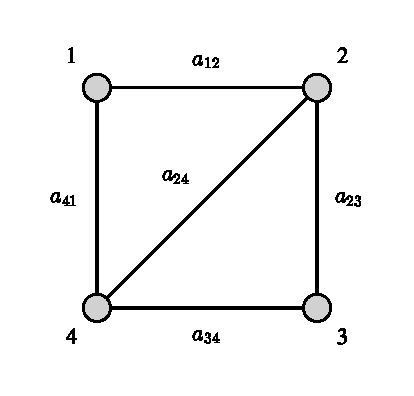
\includegraphics[width=0.72\textwidth]{fig_6.8.pdf}
\caption*{图 6.8\quad 带一条对角链的正方形上的 U(1) 规范理论。}
\end{figure}

然后我们积掉 $a_{0}$，得到\footnote{注意 $a_{0}(i)$ 与 $e_{ij}$ 之间的耦合具有 $\sum_{i}a_{0}(i)(e_{i,i+1}+e_{i,i-1})$ 的形式。路径积分 $\int\mathcal{D}a_{0}\,\mathrm{e}^{\mathrm{i}\int\mathrm{d}t\sum_{i}a_{0}(i)(e_{i,i+1}+e_{i,i-1})}$ 正比于 $\prod_{i,t}\delta(e_{i,i+1}(t)+e_{i,i-1}(t))$。}
\begin{equation*}
Z=\int\mathcal{D}a\,\mathcal{D}e_{ij}\,\mathrm{e}^{\mathrm{i}\int\mathrm{d}t\left(\sum_{i}\frac{e_{i,i+1}}{2J}\dot{a}_{i,i+1}-\frac{1}{4J}\sum_{i}e_{i,i+1}^{2}+g\cos\Phi\right)}\prod_{i,t}\delta\left(e_{i,i+1}+e_{i,i-1}\right) \tag{6.4.13}
\end{equation*}
上述系统的量子哈密顿量为
\begin{equation*}
H=\frac{1}{4J}\sum_{i}e_{i,i+1}^{2}-g\cos\Phi, \qquad \left[a_{i,i+1},(2J)^{-1}e_{i,i+1}\right]=\mathrm{i}\hbar.
\end{equation*}
物理希尔伯特空间由满足
\begin{equation*}
\left(e_{i,i+1}+e_{i,i-1}\right)|\text{phy}\rangle=0
\end{equation*}
的态构成。由于 $\left[e_{i,i+1}+e_{i,i-1},H\right]=0$，$H$ 在物理希尔伯特空间内部起作用。

为求系统的能级，我们注意到 $a_{ij}$ 以 $2\pi$ 为周期，而 $a_{ij}$ 的动量是 $e_{ij}/2J$。于是，$e_{ij}/2J$ 量子化为整数 $n_{ij}$。当 $g=0$ 时，系统的能级为 $J\sum_{i}n_{i,i+1}^{2}$，其中 $n_{ij}$ 满足约束 $\sum_{j=i\pm1}n_{ij}=0$。对我们的四格点系统，该约束要求 $n_{12}=n_{23}=n_{34}=n_{41}\equiv n$。能量本征态由 $n$ 标记，能量为 $E_{n}=4Jn^{2}$，与先前的计算一致。

\subsection*{问题 6.4.2}

\begin{enumerate}
\item[(a)] 把式 (6.4.10) 推广到带一条对角链的正方形（见图 6.8）。
\item[(b)] 假设 $g=0$，求基态与激发态的能量。
\end{enumerate}

\subsection*{问题 6.4.3}

\begin{enumerate}
\item[(a)] 证明：对于二维正方格子上的非紧致格点 U(1) 规范理论，固定规范后的路径积分具有如下形式：
\begin{equation*}
Z=\int\mathcal{D}a\,\mathrm{e}^{-\mathrm{i}\int\mathrm{d}t\left(\frac{1}{4J}\sum_{i,\mu=x,y}\dot{a}_{i,i+\mu}^{2}-\frac{1}{2g}\sum_{p}\Phi_{p}^{2}\right)}\prod_{i,t}\delta\left(\sum_{\mu=\pm x,\pm y}a_{i,i+\mu}\right)
\end{equation*}
\item[(b)] 证明：约束 $\sum_{\mu=\pm x,\pm y}a_{i,i+\mu}=0$ 可以通过引入一个定义在正方形上的实场 $\phi_{p}$ 来求解，并把链上的规范势写成 $a_{i,i+\mu}=\phi_{p_{1}}-\phi_{p_{2}}$，其中 $p_{1}$ 与 $p_{2}$ 是链 $(i,i+\mu)$ 两侧的两个正方形。试用 $\phi_{p}$ 场写出路径积分。
\item[(c)] 求 $\phi_{p}$ 涨落的色散关系。
\end{enumerate}

\subsection*{问题 6.4.4}

证明式 (6.4.12)。（提示：相空间路径积分由 $\int\mathcal{D}p\,\mathcal{D}q\,\mathrm{e}^{\mathrm{i}\int\mathrm{d}t[p\dot{q}-H(p,q)]}$ 给出，其中 $H(p,q)=p\dot{q}-L$ 是哈密顿量。）

\subsection{格点 U(1) 规范理论的库仑相与禁闭相}

\begin{keypoints}
\item 在 1+3 维中，当 $g/J\gg1$ 时，紧致格点 U(1) 规范理论处于库仑相；当 $g/J\ll1$ 时，处于禁闭相。
\end{keypoints}

我们知道，在 1+2 维中，由于瞬子效应，紧致 U(1) 规范理论总是处于禁闭相。本节我们将研究立方格子上的紧致 U(1) 规范理论。我们将论证，1+3 维的 U(1) 规范理论既有禁闭相，也有库仑相。

U(1) 规范理论的拉格朗日量为
\begin{equation*}
L=\frac{1}{4J}\sum_{\pmb{i},\pmb{\mu}=\pmb{x},\pmb{y},\pmb{z}}\left[\dot{a}_{\pmb{i},\pmb{i}+\pmb{\mu}}+a_{0}(\pmb{i})-a_{0}(\pmb{i}+\pmb{\mu})\right]^{2}+g\sum_{\pmb{p}}\cos(\Phi_{\pmb{p}})
\end{equation*}
我们可以把上述拉格朗日量的作用量写成下列无量纲形式：
\begin{equation*}
S=\sqrt{\frac{g}{J}}\int\mathrm{d}\tilde{t}\left(\frac{1}{4}\sum_{\pmb{i},\pmb{\mu}=\pmb{x},\pmb{y}}\left[\partial_{\tilde{t}}a_{\pmb{i},\pmb{i}+\pmb{\mu}}+\tilde{a}_{0}(\pmb{i})-\tilde{a}_{0}(\pmb{i}+\pmb{\mu})\right]^{2}+\sum_{\pmb{p}}\cos(\Phi_{\pmb{p}})\right)
\end{equation*}
（译注：原文此处求和指标为 $\pmb{\mu}=\pmb{x},\pmb{y}$，按上下文疑为 $\pmb{x},\pmb{y},\pmb{z}$ 之误。）其中 $\tilde{t}=\sqrt{gJ}\,t$ 是无量纲时间，$\tilde{a}_{0}=a_{0}/\sqrt{gJ}$ 是无量纲势。我们看到，当 $g/J\gg1$ 时，$\Phi_{\pmb{p}}$ 的涨落很弱，我们可以假定 $a_{\pmb{i}\pmb{j}}\sim0$。在这个极限下，$L$ 变成如下非紧致的 U(1) 规范理论：
\begin{equation*}
L=\frac{1}{4J}\sum_{\pmb{i},\pmb{\mu}=\pmb{x},\pmb{y},\pmb{z}}\left[\dot{a}_{\pmb{i},\pmb{i}+\pmb{\mu}}+a_{0}(\pmb{i})-a_{0}(\pmb{i}+\pmb{\mu})\right]^{2}-\frac{g}{2}\sum_{\pmb{p}}\Phi_{\pmb{p}}^{2}
\end{equation*}
这个二次型理论可以精确求解。在连续极限下，上式变为 U(1) 规范理论的标准麦克斯韦拉格朗日量。我们发现，低能下存在两个以 $\omega=c_{a}|\pmb{k}|$ 线性色散的模式，它们就是无能隙的光子。

当 $g/J\ll1$ 时，我们可以去掉 $\cos(\Phi_{\pmb{p}})$ 项。所得的二次型理论同样可以精确求解，就像上一节中所做的那样。相空间路径积分的拉格朗日量具有如下形式：
\begin{equation*}
L=\sum_{\pmb{i},\pmb{\mu}=\pmb{x},\pmb{y},\pmb{z}}\frac{e_{\pmb{i},\pmb{i}+\pmb{\mu}}}{2J}\left[\dot{a}_{\pmb{i},\pmb{i}+\pmb{\mu}}+a_{0}(\pmb{i})-a_{0}(\pmb{i}+\pmb{\mu})\right]-\sum_{\pmb{i},\pmb{\mu}=\pmb{x},\pmb{y},\pmb{z}}\frac{e_{\pmb{i},\pmb{i}+\pmb{\mu}}^{2}}{4J}+g\sum_{\pmb{p}}\cos(\Phi_{\pmb{p}})
\end{equation*}
积掉 $a_{0}$ 之后，我们得到约束
\begin{equation*}
\sum_{\pmb{\mu}=\pm\pmb{x},\pm\pmb{y},\pm\pmb{z}}e_{\pmb{i},\pmb{i}+\pmb{\mu}}=0
\end{equation*}
哈密顿量为
\begin{equation*}
H=\sum_{\pmb{i},\pmb{\mu}=\pmb{x},\pmb{y},\pmb{z}}\frac{e_{\pmb{i},\pmb{i}+\pmb{\mu}}^{2}}{4J}-g\sum_{\pmb{p}}\cos(\Phi_{\pmb{p}})
\end{equation*}
由于 $e_{\pmb{i}\pmb{j}}/2J$ 量子化为整数 $n_{\pmb{i}\pmb{j}}$，当 $g=0$ 时，能级为 $E=J\sum_{\pmb{i},\pmb{\mu}=\pmb{x},\pmb{y},\pmb{z}}n_{\pmb{i},\pmb{i}+\pmb{\mu}}^{2}$，其中 $n_{\pmb{i},\pmb{i}+\pmb{\mu}}$ 满足 $\sum_{\pmb{\mu}=\pm\pmb{x},\pm\pmb{y},\pm\pmb{z}}n_{\pmb{i},\pmb{i}+\pmb{\mu}}=0$。我们看到，$g=0$ 极限下的所有激发都是有能隙的。这些有能隙的激发是由非零的 $n_{\pmb{i}\pmb{j}}$ 构成的圈，这些圈代表电通量线。当存在一对正、负电荷时，两个电荷由一条电通量线连接，这在两个电荷之间产生线性禁闭势。因此，这个有能隙的相就是 U(1) 规范理论的禁闭相。

\subsection*{问题 6.4.5}

为证明在禁闭相中电荷之间以线性势相互作用，考虑存在电荷时的格点 U(1) 规范理论：
\begin{equation*}
L=\sum_{\pmb{i},\pmb{\mu}=\pmb{x},\pmb{y},\pmb{z}}\frac{\left[\dot{a}_{\pmb{i},\pmb{i}+\pmb{\mu}}+a_{0}(\pmb{i})-a_{0}(\pmb{i}+\pmb{\mu})\right]^{2}}{4J}+g\sum_{\pmb{p}}\cos(\Phi_{\pmb{p}})-\sum a_{0}(\pmb{i})q_{\pmb{i}}
\end{equation*}
其中 $q_{\pmb{i}}$ 是格点 $\pmb{i}$ 上的 U(1) 电荷。
\begin{enumerate}
\item[(a)] 求相空间路径积分中的拉格朗日量。
\item[(b)] 证明：积掉 $a_{0}$ 导出如下约束：
\begin{equation*}
\sum_{\pmb{\mu}=\pm\pmb{x},\pm\pmb{y},\pm\pmb{z}}e_{\pmb{i},\pmb{i}+\pmb{\mu}}=2Jq_{\pmb{i}}
\end{equation*}
这就是格点上的高斯定律。
\item[(c)] 假设 $g=0$，求在 $\pmb{i}=0$ 处有电荷 $q=1$、在 $\pmb{i}=l\pmb{x}$ 处有电荷 $q=-1$ 的规范理论的基态能量。证明两个电荷之间的相互作用能随 $l$ 线性增长。
\end{enumerate}

 % 本文件由 scripts/assemble.py 自动装配，勿手改（改 parts/ 后重跑）
% 第7章 量子霍尔态理论

% 第7章 THEORY OF QUANTUM HALL STATES
% 块界说明：本块自章首起，无 A-TAIL/JOIN。
% 书页 287（p302）末句 “...then it is easy to” 跨页延续至书页 288（p303）顶部
% “understand why it has a filling fraction ν=1/3.”，按约定半句译文留在本文件正文最后，
% 由下一块（ch7_b）的 A-TAIL 接续。
\chapter{量子霍尔态理论}

\begin{keypoints}
\item 分数量子霍尔液体代表着一些新的物质态，它们含有极为丰富的内部结构。
\item 不同的分数量子霍尔液体无法用序参量和局域算符的长程序来刻画。我们需要一套全新的理论来描述分数量子霍尔液体。
\item 分数量子霍尔液体含有无能隙的边缘激发，这些边缘激发构成所谓的手征 Luttinger 液体。边缘处的手征 Luttinger 液体也具有非常丰富的结构，这是体内丰富内部结构的一种反映。
\end{keypoints}

分数量子霍尔（FQH）效应出现在强磁场中的二维电子系统里。自 1982 年被发现以来（Tsui et al., 1982; Laughlin, 1983），对 FQH 系统的实验不断揭示出许多新现象和意外之处。所观察到的丰富分级（hierarchical）结构（Haldane, 1983; Halperin, 1984）表明，展示分数量子霍尔效应的电子态（这些态称为 FQH 液体）含有极为丰富的内部结构。事实上，FQH 液体代表着一种全新的物质态，它与前几章讨论过的对称性破缺态非常不同。要理解这种新的态，人们需要发展新的概念和新的技术。在本章中，我们将介绍 FQH 态的一般理论。对 FQH 态中新序（即拓扑序）的详细讨论将在第 8 章给出。

\section{阿哈罗诺夫--玻姆效应与分数统计}

\subsection{阿哈罗诺夫--玻姆效应——不接触而使粒子偏转}

\begin{keypoints}
\item 可缩回路（contractible loop）的局域相位与不可缩回路（non-contractible loop）的整体相位。
\item 非零的局域相位代表一种力，而非零的整体相位不对应任何经典的力。
\end{keypoints}

\begin{figure}[H]
\centering
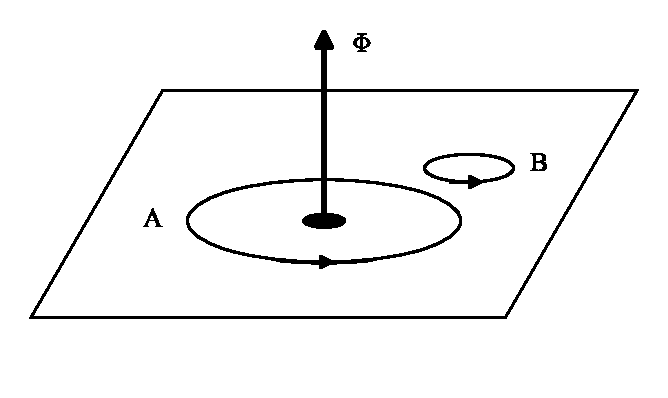
\includegraphics[width=0.72\textwidth]{fig_7.1.pdf}
\caption*{图 7.1\quad 挖去了 $\pmb{r}=0$ 点的平面，在 $\pmb{r}=0$ 处有一根磁通管。回路 $A$ 不可缩，缠绕数 $n_w=1$；回路 $B$ 可缩。}
\end{figure}

为了给以后关于量子霍尔（QH）态中量子干涉的讨论做准备，让我们先简短地讨论一下阿哈罗诺夫--玻姆（A--B）效应。首先，我们想引入两个概念，即局域相位（local phase）与整体相位（global phase）。局域相位与可缩回路相联系。把一个带电粒子沿一条可缩回路缓慢地移动一周，会产生如下的局域相位：
\begin{equation*}
\text{局域相位} = \exp\left(\mathrm{i}e\oint\pmb{A}\,\mathrm{d}\pmb{x}\right) = \exp\left(\mathrm{i}e\int\pmb{B}\cdot\mathrm{d}\pmb{S}\right).
\end{equation*}
磁场 $\pmb{B}=0$ 当且仅当所有可缩回路的局域相位都为零。因此，不受磁力作用的带电粒子没有局域相位。

整体相位则与不可缩回路相关。为了在一个简单的背景中理解整体相位，让我们考虑一个在二维平面上运动的带电粒子。我们挖去 $\pmb{r}=0$ 点，这改变了空间的拓扑。然后在 $\pmb{r}=0$ 处放置一根无穷细的磁通管，其磁通为 $\Phi$（见图 7.1）。当粒子绕 $\pmb{r}=0$ 一周时，会产生一个相位 $\mathrm{e}^{\mathrm{i}e\Phi}$。这样的相位称为整体相位。更一般地，
\begin{gather*}
\text{整体相位} = \mathrm{e}^{\mathrm{i}e\Phi n_w}\\
n_w = \text{缠绕数}.
\end{gather*}

显然，尽管整体相位非零，粒子却感受不到任何磁力，因为在远离 $\pmb{r}=0$ 处没有磁场。我们看到，一个自由粒子（即不受力的粒子）可以具有非零的整体相位。

只有当不可缩回路存在时（即空间非单连通时），整体相位才会存在。非单连通空间的另一个例子是环面（见图 7.2）。环面上的自由粒子同样可以具有整体相位。

上述自由粒子（在 $\pmb{r}=0$ 处有一根磁通管）可以用如下哈密顿量描述：
\begin{equation*}
H = -\frac{1}{2m}\left(\pmb{\partial}-\mathrm{i}\pmb{a}\right)^2, \qquad (a_x, a_y) = \frac{1}{r^2}(-y, -x)\frac{\phi}{2\pi}
\end{equation*}

\begin{figure}[H]
\centering
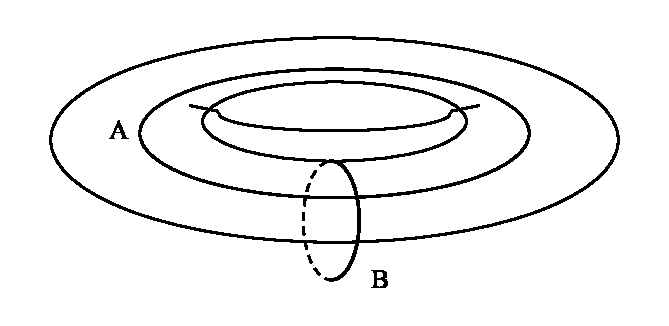
\includegraphics[width=0.72\textwidth]{fig_7.2.pdf}
\caption*{图 7.2\quad 带有两个不可缩回路 $A$ 和 $B$ 的环面。}
\end{figure}

\begin{figure}[H]
\centering
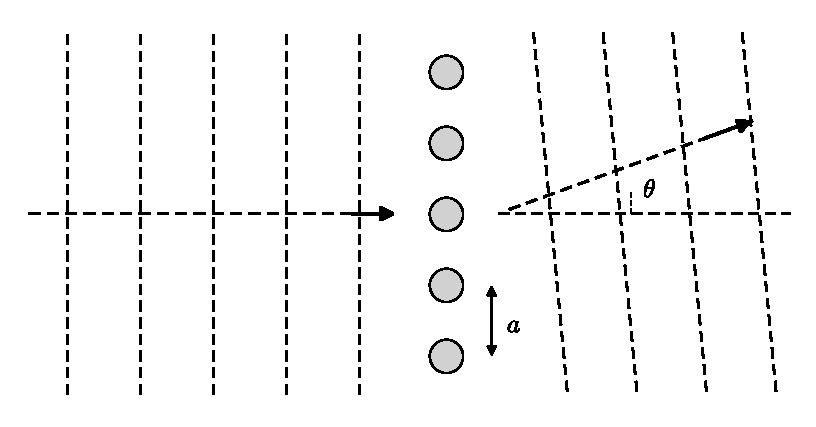
\includegraphics[width=0.72\textwidth]{fig_7.3.pdf}
\caption*{图 7.3\quad 一束粒子穿过一排管子，每根管子中都有磁通。}
\end{figure}

场强为零，即
\begin{equation*}
\pmb{b} = \partial_x a_y - \partial_y a_x = 0 \ \Longrightarrow\ \text{局域相位} = 0
\end{equation*}
对于绕 $\pmb{x}=0$ 一周的回路，我们有
\begin{equation*}
\oint\pmb{a}\cdot\mathrm{d}\pmb{x} = \phi \ \Longrightarrow\ \text{整体相位} \neq 0\ .
\end{equation*}

非零的局域相位会影响经典的运动方程。自旋的贝里相就是局域相位的一个例子（见 2.3 节）。与之相反，整体相位不会影响经典的运动方程，但它会影响粒子的量子性质。

\subsection*{问题 7.1.1}

\textbf{不接触而使其偏转}\quad 尽管整体相位不产生任何经典的力，它仍然能使一个运动的粒子偏转。考虑图 7.3 中的装置：一束电荷为 $e$、动量为 $\pmb{k}$ 的粒子穿过一排不可穿透的管子。若每根管子中都有磁通 $\Phi$，试计算偏转角 $\theta$。

\begin{figure}[H]
\centering
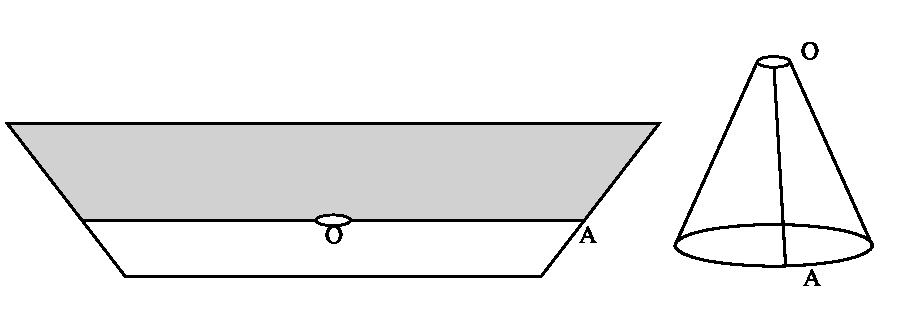
\includegraphics[width=0.72\textwidth]{fig_7.4.pdf}
\caption*{图 7.4\quad $V_-$ 空间：挖去 $\pmb{r}=0$ 点，并把 $\pmb{r}$ 与 $-\pmb{r}$ 认同为同一个点。}
\end{figure}

\subsection{具有硬芯条件的粒子与分数统计}

\begin{keypoints}
\item 具有硬芯条件的粒子，其位形空间不是单连通的。位形空间的非平凡拓扑允许非平凡的统计。
\item 分数统计存在，而且只存在于二维空间之中。
\end{keypoints}

A--B 效应的一个具体体现是二维中的分数统计（Leinaas and Myrheim, 1977; Wilczek, 1982）。考虑二维中两个自由的、具有硬芯的全同粒子。\footnote{这里，所谓自由粒子，是指彼此分开时不受任何力作用的粒子；但这些粒子可以受到硬芯条件的约束。}其位形空间由下式给出：
\begin{equation*}
\begin{aligned}
\text{位形空间} &= \left\{(\pmb{r}_1, \pmb{r}_2)\big|_{\pmb{r}_1\neq\pmb{r}_2,\ (\pmb{r}_1,\pmb{r}_2)\sim(\pmb{r}_2,\pmb{r}_1)}\right\}\\
&= \left\{(\pmb{r}_+, \pmb{r}_-)\big|_{\pmb{r}_-\neq 0,\ (\pmb{r}_+,\pmb{r}_-)\sim(\pmb{r}_-,-\pmb{r}_-)}\right\} = V_+\otimes V_-.
\end{aligned}
\end{equation*}
其中 $\pmb{r}_+=\frac{1}{2}(\pmb{r}_1+\pmb{r}_2)$，$\pmb{r}_-=\pmb{r}_1-\pmb{r}_2$，$V_+=\{\pmb{r}_+\}$，而 $V_-=\{\pmb{r}_-|_{\pmb{r}_-\neq 0,\ \pmb{r}_-\sim-\pmb{r}_-}\}$（见图 7.4）。这里 $V_+$ 是通常的二维平面，而 $V_-$ 只是二维平面的一半，因为 $\pmb{r}_-$ 与 $-\pmb{r}_-$ 被视为同一个点。同时，$\pmb{r}_-=0$ 点已从 $V_-$ 中挖去。

如上一节所指出的，“自由”意味着局域相位为零。由于两粒子位形空间不是单连通的（$V_-$ 非单连通），整体相位存在，并且我们有权自由选择整体相位。注意，$V_-$ 中的不可缩回路由缠绕数（winding number）$n_w$ 标记（图 7.5）。于是，我们可以给不可缩回路指派如下整体相位：
\begin{equation*}
\text{整体相位} = \mathrm{e}^{\mathrm{i}\theta n_w}
\end{equation*}

现在很清楚，在量子力学中存在不同种类的自由全同粒子，由一个参数 $\theta$ 标记。

\begin{figure}[H]
\centering
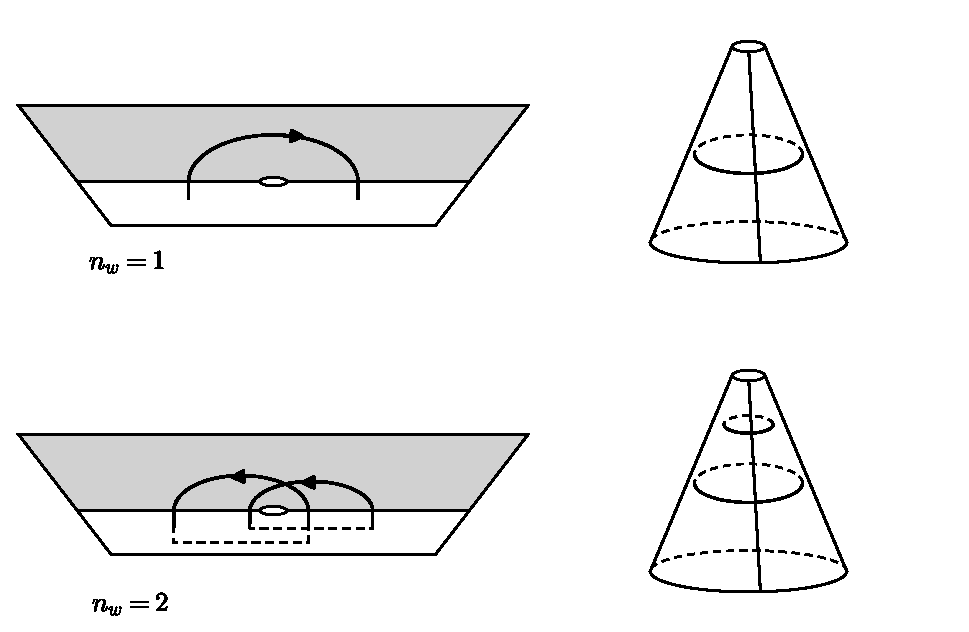
\includegraphics[width=0.72\textwidth]{fig_7.5.pdf}
\caption*{图 7.5\quad $V_-$ 空间中缠绕数 $n_w=1$ 与 $n_w=2$ 的两个回路。}
\end{figure}

\begin{itemize}
\item 参数 $\theta$ 描述多粒子位形空间中的磁通（即整体相位）。
\item 参数 $\theta$ 决定统计性质。
\end{itemize}

注意，$n_w=1$ 的回路把 $\pmb{r}_-$ 连接到 $-\pmb{r}_-$，即把 $(\pmb{r}_1,\pmb{r}_2)$ 连接到 $(\pmb{r}_2,\pmb{r}_1)$，这对应于交换两个粒子。于是，粒子的统计如下：
\begin{equation*}
\left\{\begin{array}{ccc}
\theta = 0 & \rightarrow & \text{玻色子}\\
\theta = \pi & \rightarrow & \text{费米子}\\
\theta = \text{其他} & \rightarrow & \text{任意子}
\end{array}\right.
\end{equation*}

上述两个自由全同粒子（即两个具有统计 $\theta$ 的任意子（anyon））的哈密顿量为
\begin{gather*}
H = -\frac{1}{2m}(\partial_{\pmb{r}_+})^2 - \frac{1}{2}\frac{1}{m}(\partial_{\pmb{r}_-}-\mathrm{i}\pmb{a})^2\\
(a_x, a_y) = \frac{\theta}{\pi r^2}(-y, x) \tag{7.1.1}\\
\text{边界条件：}\ \ \phi(\pmb{r}_+,\pmb{r}_-) = \phi(\pmb{r}_+,-\pmb{r}_-)
\end{gather*}

当 $\theta=0$ 且 $\pmb{a}=0$ 时，$H$ 显然描述两个玻色子。对于 $\theta=\pi$，我们可以做一个规范变换
\begin{equation*}
\phi(\pmb{r}_+,\pmb{r}_-) \rightarrow \mathrm{e}^{\mathrm{i}f(\pmb{r}_-)}\phi(\pmb{r}_+,\pmb{r}_-), \qquad f(\pmb{r}) \equiv \arctan\left(\frac{x}{y}\right)
\end{equation*}

\begin{figure}[H]
\centering
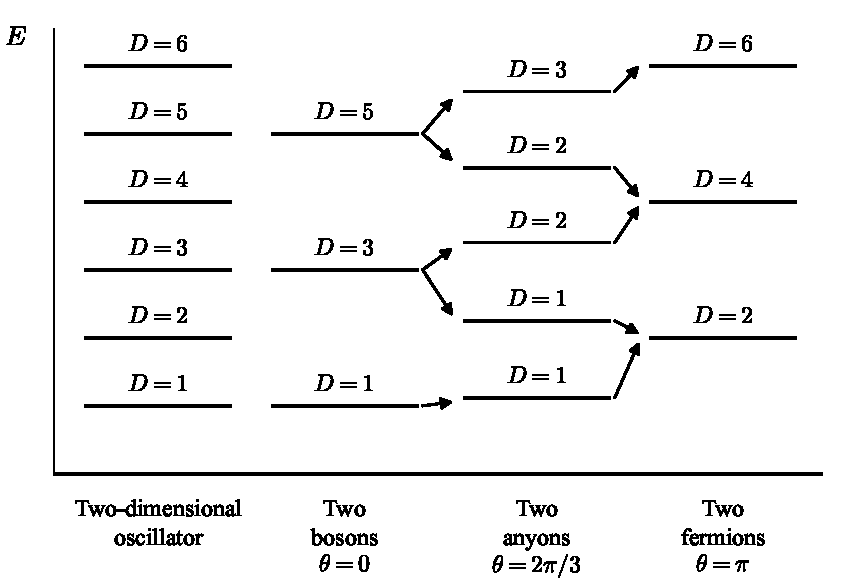
\includegraphics[width=0.72\textwidth]{fig_7.6.pdf}
\caption*{图 7.6\quad 二维谐振子势阱中两个任意子的能级 $E$ 与简并度 $D$（相对运动的）。}
\end{figure}

由于 $\nabla f(\pmb{r}) = \frac{1}{r^2}(-y, x)$，我们发现 $\mathrm{e}^{-\mathrm{i}f}(\partial_{\pmb{r}_-}-\mathrm{i}\pmb{a})^2\mathrm{e}^{\mathrm{i}f} = (\partial_{\pmb{r}_-})^2$，于是哈密顿量变为
\begin{equation*}
\begin{aligned}
H &= -\frac{1}{2m}(\partial_{\pmb{r}_+})^2 - \frac{1}{2}\frac{1}{m}(\partial_{\pmb{r}_-})^2\\
\phi(\pmb{r}_+,\pmb{r}_-) &= -\phi(\pmb{r}_+,-\pmb{r}_-)\\
\text{或}\ \ \phi(\pmb{r}_1,\pmb{r}_2) &= -\phi(\pmb{r}_2,\pmb{r}_1)
\end{aligned}
\end{equation*}
（译注：原书第二行右端误印为 $-\phi(\pmb{r}_+,\pmb{r}_-)$，此处按文意改正。）
它描述两个自由费米子。一般地说，即使是 $N$ 个费米子，我们也可以自洽地把 $\pmb{a}$ 规范掉，并通过“边界条件”（即反对称条件）来描述费米统计。然而，对于 $N$ 任意子系统，我们无法把 $\pmb{a}$ 规范掉、再用“边界条件”来表示分数统计。

我们可以求解二维谐振子势阱中的两个任意子系统，得到如图 7.6 所示的能谱。可以清楚地看到，能谱如何从玻色情形连续地变到费米情形。

一个有趣的问题是：三维中存在任意子吗？三维中两个全同自由粒子的位形空间为 $V_+^{(3D)}\otimes V_-^{(3D)}$，其中
\begin{equation*}
V_-^{(3D)} = \left\{\pmb{r}_-\big|_{\pmb{r}_-\neq 0,\ \pmb{r}_-\sim-\pmb{r}_-}\right\}
\end{equation*}
这里 $V_-^{(3D)}$ 不是单连通的，整体相位存在。然而，$V_-^{(3D)}$ 中的不可缩回路由 $Z_2$ 标记。

\begin{figure}[H]
\centering
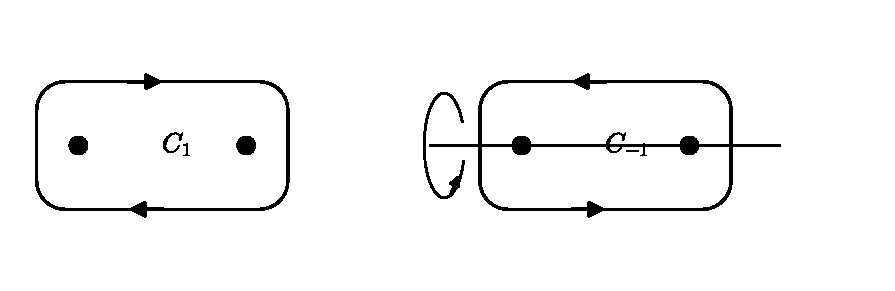
\includegraphics[width=0.72\textwidth]{fig_7.7.pdf}
\caption*{图 7.7\quad 两个交换回路 $C_1$ 与 $C_{-1}$ 在三维中可以通过绕连接两粒子的轴转动而连续地相互变换。}
\end{figure}

\begin{figure}[H]
\centering
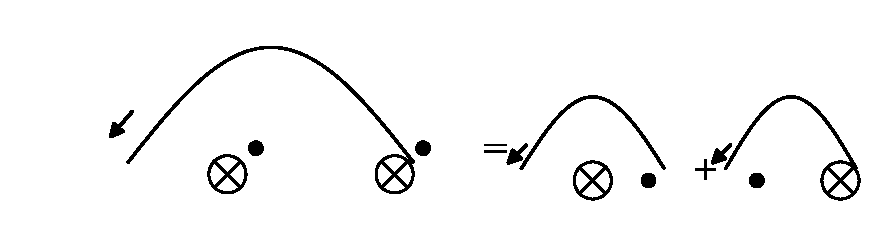
\includegraphics[width=0.72\textwidth]{fig_7.8.pdf}
\caption*{图 7.8\quad 把一个通量--电荷束缚态绕另一个通量--电荷束缚态移动一周所诱导的相位。}
\end{figure}

这是因为沿一个方向的交换（由回路 $C_1$ 描述）与沿相反方向的交换（由回路 $C_{-1}$ 描述）属于同一类，因为两条回路 $C_{\pm 1}$ 可以连续地相互变形（见图 7.7）。如果我们给回路 $C_1$ 指派整体相位 $\mathrm{e}^{\mathrm{i}\theta}$，那么回路 $C_{-1}$ 将具有整体相位 $\mathrm{e}^{-\mathrm{i}\theta}$。由于两条回路 $C_{\pm 1}$ 仅相差一个局域相位为零的可缩回路，我们还有 $\mathrm{e}^{\mathrm{i}\theta}=\mathrm{e}^{-\mathrm{i}\theta}$。因此，$\theta$ 只能取如下两个可能的值：
\begin{equation*}
\theta = \left\{\begin{array}{cl}
0, & \text{玻色子}\\
\pi, & \text{费米子}
\end{array}\right.
\end{equation*}

以上的讨论表明，任意子是量子力学中的一种数学可能性。下一个问题是：任意子怎样才能出现在一些原本不含任意子的物理模型中？事实上，任意子可以作为玻色子/费米子系统中的激发出现。下面我们将考虑一个任意子作为电荷与磁通的束缚态而出现的模型。考虑一个由电荷为 1 的玻色子 $\phi$ 组成的系统。假设玻色子形成 $q$ 玻色子束缚态 $\Phi_q=(\phi)^q$，且 $\Phi_q$ 发生玻色凝聚。有效拉格朗日量为
\begin{align*}
\mathcal{L}_{\text{eff}} ={}& \frac{1}{2}\left|(\partial_\mu-\mathrm{i}q a_\mu)\Phi_q\right|^2 - \frac{1}{2}a\left|\Phi_q\right|^2 - \lambda\left|\Phi_q\right|^4 + \frac{1}{2g}\left(f_{\mu\nu}\right)^2 \tag{7.1.2}\\
&\qquad\qquad \langle\Phi_q\rangle \neq 0
\end{align*}
其中 $a_\mu$ 是与电荷玻色子耦合的 $U(1)$ 规范场。在凝聚态中，涡旋携带磁通 $\frac{2\pi}{q}$（见问题 7.1.2）。考虑涡旋 $\frac{2\pi}{q}$ 与原来的玻色子 $\phi$ 的束缚态。把一个束缚态绕另一个束缚态半周，我们得到一个相位
\begin{equation*}
\theta = \frac{1}{2}\frac{2\pi}{q} + \frac{1}{2}\frac{2\pi}{q} = \frac{2\pi}{q}
\end{equation*}
第一项来自电荷绕磁通管一周，第二项来自磁通管绕电荷一周（见图 7.8）。我们看到，$q=1$ 时束缚态是玻色子，$q=2$ 时是费米子，$q>2$ 时是任意子。

对于 BCS 超导体，$q=2$。但 $\phi$ 是费米子，因此束缚态是玻色子。目前所知唯一支持任意子激发的凝聚态系统是 FQH 系统。

\subsection*{问题 7.1.2}

在极坐标 $(r,\phi)$ 中，式 (7.1.2) 中的涡旋由
\begin{equation*}
\Phi_q = f(r)\mathrm{e}^{\mathrm{i}\phi}
\end{equation*}
描述，其中 $f(\infty)=\langle\Phi_q\rangle$。
\begin{enumerate}
\item[(a)] 证明：若 $a_\mu=0$，则涡旋的能量按 $\ln(L)$ 发散，其中 $L$ 是系统的尺寸。
\item[(b)] 求出使涡旋具有有限能量的 $\pmb{a}(r,\phi)$。
\item[(c)] 证明上述 $\pmb{a}(r,\phi)$ 的总磁通为 $2\pi/q$。
\end{enumerate}

\section{量子霍尔效应}

\subsection{整数量子霍尔效应}

\begin{keypoints}
\item 整数量子霍尔（IQH）态由填满的朗道能级描述。
\item $\nu=1$ IQH 态的多体波函数。
\item IQH 波函数的密度分布。
\end{keypoints}

让我们先讨论经典霍尔效应。考虑一个电荷 $q_e=-e$ 的电子二维气体，它在面内电场和垂直于该面的磁场的作用下运动。为了维持静态电流，电场力必须与磁场的洛伦兹力相平衡，即
\begin{equation*}
q_e\pmb{E} = q_e\pmb{v}\times\pmb{B}
\end{equation*}
在本章中，我们将选取使光速 $c=1$ 的单位。由于电流 $\pmb{j}$ 由 $\pmb{v}n$ 给出（$n$ 为密度），$\pmb{E}$ 与 $\pmb{j}$ 通过下式相联系：
\begin{equation*}
\pmb{E}\perp\pmb{j}, \qquad |\pmb{E}| = |\pmb{j}|\frac{B}{nq_ec} = |\pmb{j}|\frac{h}{q_e^2}\frac{B/(hc/q_e)}{n} = |\pmb{j}|\left(\frac{h}{q_e^2}\right)\frac{1}{\nu}
\end{equation*}
其中
\begin{equation*}
\nu \equiv \frac{nhc}{q_eB} = \frac{\text{粒子数}}{\text{磁通量子数}}
\end{equation*}
\begin{figure}[H]
\centering
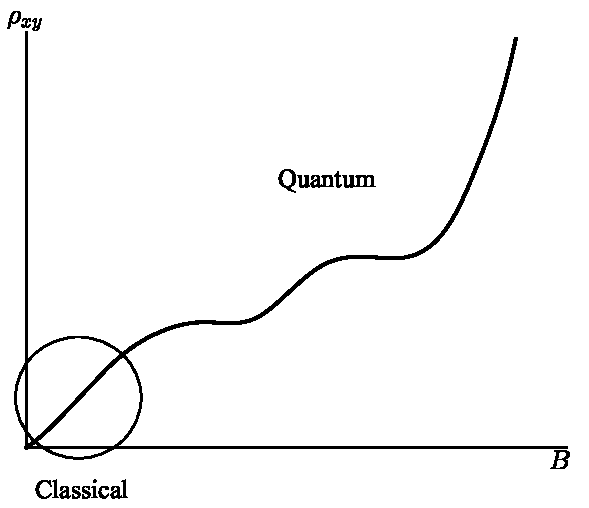
\includegraphics[width=0.72\textwidth]{fig_7.9.pdf}
\caption*{图 7.9\quad 霍尔电阻 $\rho_{xy}$ 随 $B$ 的变化。}
\end{figure}
为填充因子。霍尔电阻 $\rho_{xy}=\left(\frac{h}{q_e^2}\right)\frac{1}{\nu}$ 可以在实验中直接测量。按照上述经典理论，若 $n$ 固定，则 $\rho_{xy}\propto B$。

实验上确实发现，对于二维电子气体，弱场下 $\rho_{xy}\propto B$（见图 7.9）。20 世纪 80 年代初，物理学家把二维电子气体置于强磁场（$\sim$10 特斯拉）中并冷却到极低的温度（$\sim$1 K），发现对于强 $B$，$\rho_{xy}$ 呈现平台结构，如图 7.9 所示（von Klitzing et al., 1980; Tsui et al., 1982）。这一现象称为 QH 效应。物理学家很快发现了 QH 态的许多惊人性质。最令人惊讶的是，平台恰好出现在与下式对应的那些 $\rho_{xy}$ 处：
\begin{equation*}
\nu = \underbrace{1, 2, 3, \cdots}_{\text{IQH}},\ \underbrace{\frac{1}{3}, \frac{2}{3}, \frac{2}{5}, \frac{3}{7}, \cdots}_{\text{FQH}}
\end{equation*}
$\rho_{xy}$ 的值如此精确和稳定，以致它已成为电阻的标准。

平台背后的物理稍微复杂一些，因为它涉及杂质。简而言之，如果二维电子气体在这些 $\nu$ 值处形成不可压缩液体\footnote{即所有带电激发都具有有限的能隙。}，我们就能理解这些填充因子处的平台。下面我们将看到，由于朗道能级结构，电子在 $\nu=1,2,3,\cdots$ 处确实形成不可压缩态。这使我们能够理解整数 $\nu$ 处的平台以及整数量子霍尔效应。

让我们忽略库仑相互作用，考虑强磁场 $B$ 中的二维自由电子气体。我们将忽略电子自旋，或者假设电子自旋已被极化。均匀磁场中的单个电子由下式描述：
\begin{gather*}
H = -\frac{1}{2m}(\partial_i-\mathrm{i}q_eA_i)^2, \qquad \hbar = c = 1 \tag{7.2.1}\\
(A_x, A_y) = \frac{B}{2}(-y, x), \qquad \text{（对称规范）}\\
B = \partial_xA_y - \partial_yA_x
\end{gather*}

上述哈密顿量有一个有趣的对称性质。尽管磁场是均匀的，它在直接平移 $T_{\pmb{a}}=\mathrm{e}^{-\pmb{a}\cdot\pmb{\partial}_{\pmb{x}}}$ 下却并非不变，即 $T_{\pmb{a}}HT_{\pmb{a}}^{\dagger}\neq H$。然而，在平移 $T_{\pmb{a}}$ 之后接着做规范变换
\begin{equation*}
G_{\pmb{a}} = \mathrm{e}^{\mathrm{i}\frac{1}{2}Bq_e(xa^y-ya^x)} \tag{7.2.2}
\end{equation*}
它就是不变的；或者更精确地说，
\begin{equation*}
G_{\pmb{a}}T_{\pmb{a}}H(G_{\pmb{a}}T_{\pmb{a}})^{\dagger} = H
\end{equation*}
组合变换 $G_{\pmb{a}}T_{\pmb{a}}$ 是 $H$ 的一个对称性，称为磁平移。不同方向的磁平移互不对易：
\begin{equation*}
(G_{\pmb{a}}T_{\pmb{a}})(G_{\pmb{b}}T_{\pmb{b}}) = \mathrm{e}^{-\mathrm{i}q_eB(a^xb^y-a^yb^x)}(G_{\pmb{b}}T_{\pmb{b}})(G_{\pmb{a}}T_{\pmb{a}}) \tag{7.2.3}
\end{equation*}
因此，尽管哈密顿量在 $x$、$y$ 两个方向都有磁平移对称性，$H$ 的本征态却不能用动量矢量 $(k_x,k_y)$ 来标记。注意，相位 $q_eB(a^xb^y-a^yb^x)$ 恰好是把电荷 $q_e$ 沿由 $\pmb{a}$、$\pmb{b}$ 张成的平行四边形 $P_{\pmb{a}\pmb{b}}$ 绕一周所得到的相位，即 $\mathrm{e}^{\mathrm{i}q_e\oint_{P_{\pmb{ab}}}\mathrm{d}\pmb{x}\cdot\pmb{A}}$。

为了求出式 (7.2.1) 的能级，我们引入复坐标 $z=x+\mathrm{i}y$，于是
\begin{equation*}
\left\{\begin{array}{ll}
\partial_z = \frac{1}{2}(\partial_x-\mathrm{i}\partial_y), & x = \frac{1}{2}(z+\bar{z}),\\
\partial_{\bar{z}} = \frac{1}{2}(\partial_x+\mathrm{i}\partial_y), & y = \frac{1}{2\mathrm{i}}(z-\bar{z}).
\end{array}\right.
\end{equation*}
用 $z$ 与 $\bar{z}$ 表示，我们有
\begin{equation*}
H = -\frac{1}{m}(D_zD_{\bar{z}} + D_{\bar{z}}D_z)
\end{equation*}
其中
\begin{equation*}
\left\{\begin{array}{ll}
D_z = \partial_z-\mathrm{i}q_eA_z, & A_z = \frac{1}{2}(A_x-\mathrm{i}A_y) = \frac{B}{4\mathrm{i}}\bar{z}\\
D_{\bar{z}} = \partial_{\bar{z}}-\mathrm{i}q_eA_{\bar{z}}, & A_{\bar{z}} = \frac{1}{2}(A_x+\mathrm{i}A_y) = -\frac{B}{4\mathrm{i}}z
\end{array}\right.
\end{equation*}
哈密顿量 $H$ 可以通过一个非幺正变换 $\mathrm{e}^{+|z|^2/4l_B^2}$ 来简化，其中 $l_B$ 是磁长度，定义为
\begin{equation*}
l_B^2 = \left|\frac{c\hbar}{q_eB}\right|
\end{equation*}
（注意 $2\pi l_B^2B = \frac{hc}{q_e} = \Phi_0$ 给出一个单位磁通量子。）我们发现
\begin{equation*}
H = \mathrm{e}^{-|z|^2/4l_B^2}\left[-\frac{1}{m}\left(\tilde{D}_z\tilde{D}_{\bar{z}} + \tilde{D}_{\bar{z}}\tilde{D}_z\right)\right]\mathrm{e}^{+|z|^2/4l_B^2}
\end{equation*}
其中
\begin{align*}
\tilde{D}_z &= \mathrm{e}^{+|z|^2/4l_B^2}D_z\mathrm{e}^{-|z|^2/4l_B^2} = \partial_z - \frac{q_eB}{4c}\bar{z} - \frac{1}{4l_B^2}\bar{z} = \partial_z - \frac{1}{2l_B^2}\bar{z}\\
\tilde{D}_{\bar{z}} &= \partial_{\bar{z}} + \frac{q_eB}{4c}z - \frac{1}{4l_B^2}z = \partial_{\bar{z}}
\end{align*}
这里我们假定了 $q_eB>0$。我们看到，非幺正变换 $\mathrm{e}^{+|z|^2/4l_B^2}$ 可以看作一个使 $A_{\bar{z}}=0$ 的“规范变换”。我们可以进一步把 $H$ 简化为
\begin{equation*}
H = \mathrm{e}^{-|z|^2/4l_B^2}\left[-\frac{2}{m}\left(\partial_z-\frac{1}{2l_B^2}\bar{z}\right)\partial_{\bar{z}}\right]\mathrm{e}^{+|z|^2/4l_B^2} + \frac{1}{2}\hbar\omega_c
\end{equation*}
其中 $\omega_c=q_eB/mc$ 是回旋频率。

现在我们可以容易地写出均匀磁场中电子的本征态：
\begin{equation*}
\begin{array}{ll}
\Psi_0 = \mathrm{e}^{-|z|^2/4l_B^2}f(z) & E = \frac{1}{2}\hbar\omega_c\\[5pt]
\Psi_1 = \mathrm{e}^{-|z|^2/4l_B^2}\left(\partial_z-\frac{1}{2l_B^2}\bar{z}\right)f(z) & E = \left(\frac{1}{2}+1\right)\hbar\omega_c\\[5pt]
\Psi_n = \mathrm{e}^{-|z|^2/4l_B^2}\left(\tilde{D}_z\right)^n f(z) & E = \left(\frac{1}{2}+n\right)\hbar\omega_c
\end{array}
\end{equation*}
这给出了朗道能级结构。

在上面的讨论中我们假定了 $q_eB>0$。第零朗道能级中的电子波函数是解析函数 $f(z)$ 乘以 $\mathrm{e}^{-|z|^2/4l_B^2}$。若 $q_eB<0$，则非幺正变换 $\mathrm{e}^{+|z|^2/4l_B^2}$ 将把 $A^z$ 变为零，第零朗道能级中的电子波函数将是反解析函数 $f(z^*)$ 乘以 $\mathrm{e}^{-|z|^2/4l_B^2}$。

第零朗道能级中的波函数 $\Psi_0$ 可以用基态
\begin{equation*}
\psi_m = \sqrt{N_m}\,z^m\,\mathrm{e}^{-|z|^2/4l_B^2}
\end{equation*}
展开，它们携带角动量 $m$。波函数 $\psi_m$ 呈环状。$|\psi_m| = \mathrm{e}^{m\ln|z|-|z|^2/4l_B^2}$ 的极大值位置在
\begin{equation*}
|z| = r_m = \sqrt{2m}\,l_B
\end{equation*}
我们发现第 $m$ 个态的环所围的面积为 $\pi r_m^2 = 2\pi l_B^2 m$，其中含有 $m$ 个磁通量子（见图 7.10）。

\begin{figure}[H]
\centering
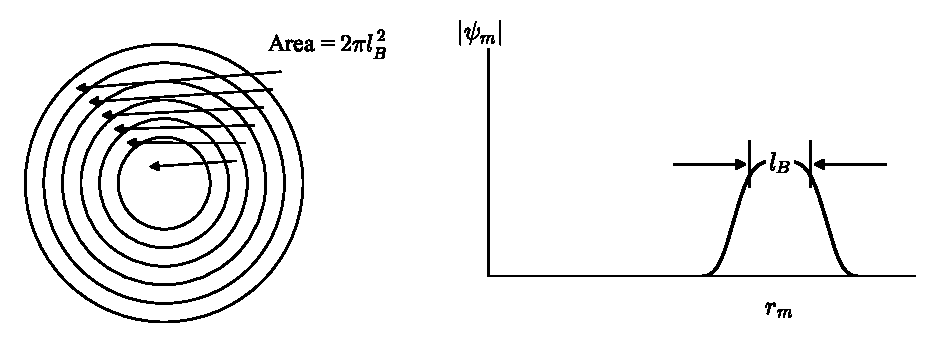
\includegraphics[width=0.72\textwidth]{fig_7.10.pdf}
\caption*{图 7.10\quad 第零朗道能级中的圆形轨道。}
\end{figure}

\begin{figure}[H]
\centering
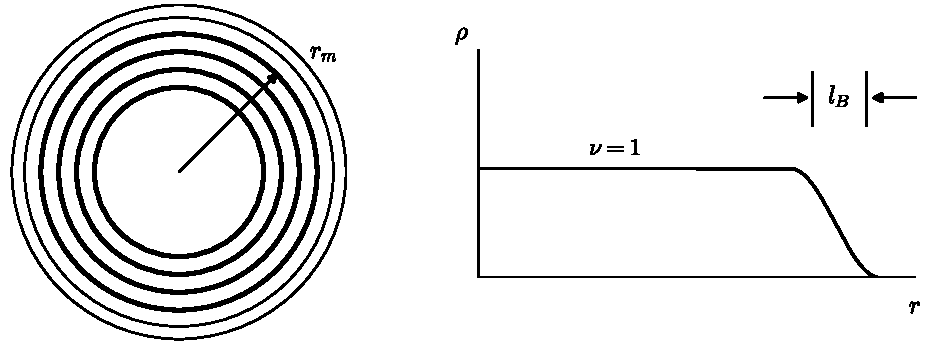
\includegraphics[width=0.72\textwidth]{fig_7.11.pdf}
\caption*{图 7.11\quad $\nu=1$ 液滴的密度分布，其中前 $m$ 个能级（由粗线表示）已被填满。}
\end{figure}

因此，每一个磁通量子对应一个态，而第零朗道能级中的态数等于磁通量子数。于是，当 $\nu=1$ 时，第零朗道能级中的每个态都被一个电子占据。这给出有限的激发能隙 $\Delta=\hbar\omega_c$，并解释了实验中观察到的 $\nu=1$ 平台。不可压缩性来源于泡利不相容原理（费米统计）。

$\nu=1$ 态的多体波函数具有如下形式：
\begin{equation*}
\begin{aligned}
\Psi(z_1,\cdots z_N) &= \mathcal{A}\left[(z_1)^0(z_2)^1(z_3)^2\cdots\right]\mathrm{e}^{-\sum|z_i|^2/4l_B^2}\\
&= \det\left|\begin{array}{ccc}
1 & 1 & \ldots\\
z_1 & z_2 & \ldots\\
(z_1)^2 & (z_2)^2 & \ldots\\
\vdots & \vdots & \vdots
\end{array}\right|\mathrm{e}^{-\sum|z_i|^2/4l_B^2} = \prod_{i<j}(z_i-z_j)\,\mathrm{e}^{-\sum|z_i|^2/4l_B^2}
\end{aligned}
\end{equation*}
其中 $\mathcal{A}$ 是反对称化算符。上述波函数描述一个具有均匀密度的圆形液滴（图 7.11），因为每个电子占据相同的面积 $\pi r_{m+1}^2-\pi r_m^2 = 2\pi l_B^2$。这个性质很重要。一个一般的 $N$ 变量波函数在 $N\to\infty$ 极限下未必具有均匀的密度；那样的波函数不具有合理的热力学极限。

\begin{figure}[H]
\centering
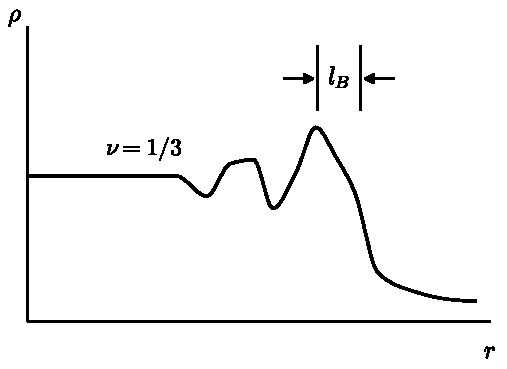
\includegraphics[width=0.72\textwidth]{fig_7.12.pdf}
\caption*{图 7.12\quad $\nu=1/3$ 液滴的密度分布。}
\end{figure}

\subsection*{问题 7.2.1}

求电子在势场 $V=\frac{1}{2}m\omega_0^2r^2$ 与均匀磁场 $B$ 中的能级。

\subsection*{问题 7.2.2}

\begin{enumerate}
\item[(a)] 证明：若规范变换 $G_{\pmb{a}}$ 由式 (7.2.2) 给出，则磁平移 $G_{\pmb{a}}T_{\pmb{a}}$ 是均匀磁场中哈密顿量 (7.2.1) 的一个对称性。
\item[(b)] 证明磁平移满足代数关系 (7.2.3)。
\end{enumerate}

\subsection{分数量子霍尔效应}

\begin{keypoints}
\item FQH 态的 Laughlin 波函数。
\item 等离子体类比与 Laughlin 态的密度分布。
\end{keypoints}

当 $0<\nu<1$ 时，第零朗道能级只是部分填充。对自由电子而言，这给出一个巨大的基态简并度 ${\sim}\,\frac{N_\phi!}{N!(N_\phi-N)!}$（其中 $N_\phi$ 是第零朗道能级中的态数，它同时也是磁通量子数；$N$ 是电子数）。因此，实验上观察到的 $\nu=1/3$ 态必定来自相互作用。这里有两个问题。第一，相互作用怎样才能产生能隙（不可压缩性）？第二，为什么 $\nu=1/3$ 是特别的？

Laughlin 用如下尝试波函数回答了上述两个问题：
\begin{equation*}
\Psi_3 = \prod_{i<j}(z_i-z_j)^3\,\mathrm{e}^{-\sum|z_i|^2/4l_B^2}
\end{equation*}
波函数 $\Psi_3$ 之所以好，有如下几条理由：
\begin{enumerate}
\item[a)] $\Psi_3$ 对每一对电子都有一个三阶零点 $(z_i-z_j)^3$。这对排斥型相互作用有利。
\item[b)] $\Psi_3$ 描述一个密度均匀的圆形液滴（图 7.12），其填充为 $\nu=1/3$。
\item[c)] $\Psi_3$ 是一个不可压缩态。
\end{enumerate}

由于 $|\Psi_3|$ 具有旋转不变性，显然 $|\Psi_3|$ 描述一个圆形液滴。如果我们再假设液滴还具有均匀的密度，那么就很容易
% ——本块到此为止：句子未完，接下一块 ch7_b（书页 288 / p303 顶部 “understand why it has a filling fraction ν=1/3.”），
% 由 ch7_b 的 A-TAIL 补出“理解它为何具有填充因子 ν=1/3。”
理解为什么它具有填充因子 $\nu=1/3$。这是因为 $z_i$（固定 $i$）的最高次幂是 $3(N-1)$。角动量为 $3(N-1)$ 的轨道的半径为 $r_{\max}=\sqrt{2\times 3(N-1)}\,l_B$。这里 $r_{\max}$ 也是液滴的半径，是 $\nu=1$ 液滴半径 $\sqrt{2\times(N-1)}\,l_B$ 的 $\sqrt{3}$ 倍。因此，对 $\Psi_3$ 有 $\nu=\frac{1}{3}$。

为了理解为什么 $\Psi_3$ 具有均匀的密度，让我们考虑下面电子位置的联合概率分布：
\begin{equation*}
P(z_1\cdots z_N)\propto|\Psi_m(z_1\cdots z_N)|^2=\mathrm{e}^{-\beta V(z_1\cdots z_N)}
\tag{7.2.4}
\end{equation*}
其中我们已把 $\Psi_3$ 态推广为 $\Psi_m$ 态
\begin{equation*}
\Psi_m=\prod_{i<j}(z_i-z_j)^m\,\mathrm{e}^{-\sum|z_i|^2/4l_B^2}
\end{equation*}
我们看到，为使 $\Psi_m$ 全反对称，$m$ 必须是奇整数。在式 (7.2.4) 中选择 $T=\frac{1}{\beta}=\frac{m}{2}$，我们可以把
\begin{equation*}
V=-m^2\sum_{i<j}\ln|z_i-z_j|+\frac{m}{4l_B^2}\sum_i|z_i|^2
\end{equation*}
视为由带"电荷" $m$ 的粒子组成的二维等离子体的势，而把 $P(z_1\cdots z_N)$ 视为该等离子体的概率分布。"电荷"为 $m_1$ 与 $m_2$ 的两个粒子之间的势是 $-m_1m_2\ln(r)$，力是 $m_1m_2/r$。因此，要理解 $\Psi_m$ 的密度分布，我们只需计算等离子体的"电荷"分布。

在 $V$ 中我们看到，等离子体中的每个粒子感受到一个势 $m|z|^2/4l_B^2$，它可以视为由一个背景"电荷"分布产生的势。实际上，这样的势由"电荷"密度为 $\rho_\phi=1/2\pi l_B^2$ 的均匀背景"电荷"产生，这正好就是磁通量子的密度。为看出这一点，我们注意到，这样的背景"电荷"作用在半径 $r$ 处的"电荷" $m$ 上的力，是"电荷" $m$ 与半径 $r$ 之内总"电荷"之间的力。该力由 $F=m\rho_\phi\pi r^2/r=m\rho_\phi\pi r$ 给出。这给出一个势 $\frac{m}{2}\pi\rho_\phi r^2$，正好就是上面的势。由于等离子体的完全屏蔽性质，等离子体倾向于"电荷"中性。等离子体的"电荷"密度等于背景"电荷"密度 $mn_e=\rho_\phi$，其中 $n_e$ 是电子密度。我们得到填充因子 $\nu=n_e/\rho_\phi=\frac{1}{m}$。

为什么 $\Psi_m$ 是不可压缩态？注意到 $\Psi_m$ 的总角动量（$z_i$ 的总幂次）为 $M_0=m\frac{N(N-1)}{2}$。$\Psi_m$ 是具有最小总角动量的态，它在每一对电子之间都有 $m$ 阶零点。压缩液滴会减小总角动量并产生更低阶的零点，这要耗费能量。我们预期该能隙为库仑能 $e^2/l_B$ 的量级。上述论断没有数学证明，但我们有大量的数值证据。

我们想指出，虽然对具有库仑相互作用的电子而言 $\Psi_3$ 只是近似基态，但存在一个理想哈密顿量，使 $\Psi_3$ 成为它的精确基态。理想哈密顿量具有形式
\begin{equation*}
H=\frac{1}{2m}\sum_i(\partial_{\pmb{x}_i}-\mathrm{i}q_e\pmb{A})^2-\sum_{i<j}UV(\pmb{r}_i-\pmb{r}_j),\quad V(\pmb{r})=\partial_{\pmb{r}}^2\delta(\pmb{r}).
\tag{7.2.5}
\end{equation*}
可以证明，对任意态 $\psi$ 有 $\langle\psi|H|\psi\rangle\geqslant\frac{1}{2}N\hbar\omega_c$，而对 $\Psi_3$ 有 $\langle\Psi_3|H|\Psi_3\rangle=\frac{1}{2}N\hbar\omega_c$。因此 $\Psi_3$ 确实是 $H$ 的精确基态。数值计算还表明，对理想哈密顿量而言 $\Psi_3$ 是不可压缩的。

\subsection*{问题 7.2.3}

证明：对理想哈密顿量 (7.2.5) 有 $\langle\Psi_3|H|\Psi_3\rangle=\frac{1}{2}N\hbar\omega_c$。为 $\nu=1/m$ 的 Laughlin 态 $\Psi_m$ 找一个理想哈密顿量。

\subsection*{问题 7.2.4}

双层 FQH 态由波函数
\begin{equation*}
\Psi_{lmn}=\prod_{i<j}(z_i-z_j)^l\prod_{i<j}(w_i-w_j)^m\prod_{i,j}(z_i-w_j)^n\,\mathrm{e}^{-\sum|z_i|^2/4l_B^2}\,\mathrm{e}^{-\sum|w_i|^2/4l_B^2}
\tag{7.2.6}
\end{equation*}
描述，其中 $z_i$ 是第一层中电子的坐标，$w_i$ 是第二层中电子的坐标。这样的态称为 $(lmn)$ 态。设 $N_1$ 与 $N_2$ 为两层中的电子数。求使两层中电子液滴尺寸相等的比值 $N_1/N_2$。求两层中电子的总填充因子。（提示：可先假设 $n=0$ 以简化问题。）

\subsection{具有分数电荷与分数统计的准粒子}

\begin{keypoints}
\item 由等离子体类比得到的分数电荷与分数统计。
\end{keypoints}

不可压缩基态 $\Psi_m$ 之上的准空穴激发由多体波函数
\begin{equation*}
\Psi^h(\xi,\xi^*)=\sqrt{C(\xi,\xi^*)}\prod_i(\xi-z_i)\Psi_m,
\end{equation*}
描述，其中 $\xi$ 是准空穴的位置，$C(\xi,\xi^*)$ 是归一化系数。计算准空穴电荷最简单的方式，是先从 $\Psi_m$ 态中移除一个电子，得到波函数 $\prod_i(\xi-z_i)^m\Psi_m$，它在 $\xi$ 处有一个电荷为 $e$ 的空穴。然而，$\prod_i(\xi-z_i)^m\Psi_m$ 也可以视为在 $\xi$ 处有 $m$ 个准空穴的波函数。因此，准空穴携带的电荷是 $e/m$。

\begin{figure}[H]
\centering
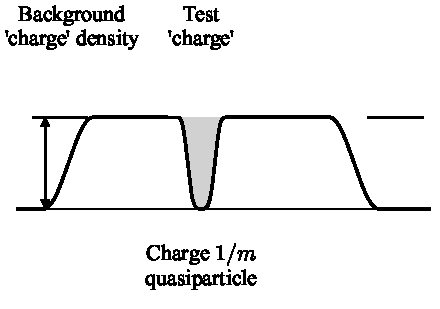
\includegraphics[width=0.72\textwidth]{fig_7.13.pdf}
\caption*{图 7.13\quad 电子的电荷与测试电荷必须中和背景电荷。}
\end{figure}

计算准空穴电荷更直接的途径是等离子体类比。准空穴态 $\Psi_h$ 中电子位置的分布为
\begin{equation*}
P^h_\xi(\{z_i\})=\bigl|\Psi^h(\xi,\xi^*)\bigr|^2=\mathrm{e}^{-\beta[V(z_i)-m\ln|\xi-z_i|]}
\end{equation*}
因此，电子感受到一个附加的背景势 $-m\ln|\xi-z_i|$。这个势由一个单位测试电荷产生。背景电荷在 $\xi$ 处包含一个额外的单位测试电荷。为维持电荷中性，$\xi$ 附近必须少 $1/m$ 个电子（见图 7.13）。这样，准空穴携带电荷 $e/m$。

为了理解准空穴的分数统计（Arovas et al., 1984），让我们从下面几个准粒子的有效拉格朗日量出发：
\begin{equation*}
Z=\int\mathcal{D}[\pmb{x}_i(t)]\;\mathrm{e}^{\mathrm{i}\int\mathrm{d}t\,\sum_i[-E_0+\frac{1}{2}m\dot{\pmb{x}}_i^2+\pmb{a}(\pmb{x}_1,\pmb{x}_2,\ldots)\cdot\dot{\pmb{x}}_i]}
\end{equation*}
有效规范势 $\pmb{a}$ 决定统计。正如 2.3 节讨论的自旋系统那样，$\pmb{a}$ 由相干态 $|\Psi^h(\xi(t),\xi^*(t))\rangle$ 的贝里相决定。

让我们先只考虑单个准粒子。对于准粒子 $\xi(t)$ 的绝热运动，$\Psi^h(\xi(t),\xi^*(t))$ 的相位变化给出贝里相。对小的 $\Delta t$，贝里相为
\begin{equation*}
\langle\Psi^h(\xi(t+\Delta t),\xi^*(t+\Delta t))|\Psi^h(\xi(t),\xi^*(t))\rangle=\mathrm{e}^{\mathrm{i}\Delta t\,\pmb{a}\cdot\dot{\pmb{x}}}.
\end{equation*}
于是 $\pmb{a}$ 由
\begin{equation*}
\mathrm{i}\langle\Psi^h(\xi(t),\xi^*(t))|\frac{\mathrm{d}}{\mathrm{d}t}|\Psi^h(\xi(t),\xi^*(t))\rangle=\pmb{a}\cdot\dot{\pmb{x}}
\end{equation*}
给出。由于 $\Psi^h$ 只通过 $\xi(t)$ 依赖 $t$，我们有
\begin{align*}
\pmb{a}\cdot\dot{\pmb{x}}&=\mathrm{i}\langle\Psi^h(\xi(t),\xi^*(t))|\frac{\mathrm{d}}{\mathrm{d}t}|\Psi^h(\xi(t),\xi^*(t))\rangle\\
&=\frac{\mathrm{d}\xi}{\mathrm{d}t}\,\mathrm{i}\langle\Psi^h(\xi,\xi^*)|\frac{\partial}{\partial\xi}|\Psi^h(\xi,\xi^*)\rangle+\frac{\mathrm{d}\xi^*}{\mathrm{d}t}\,\mathrm{i}\langle\Psi^h(\xi,\xi^*)|\frac{\partial}{\partial\xi^*}|\Psi^h(\xi,\xi^*)\rangle
\end{align*}
这样，如果我们写出 $\pmb{a}\cdot\mathrm{d}\pmb{x}=a_\xi\mathrm{d}\xi+a_{\xi^*}\mathrm{d}\xi^*$，就有\footnote{我们用到了
\[
\begin{aligned}
&\mathrm{i}\langle\Psi^h(\xi,\xi^*)|\frac{\partial}{\partial\xi}|\Psi^h(\xi,\xi^*)\rangle=\mathrm{i}\langle\Psi(\xi)|\frac{1}{\sqrt{C(\xi,\xi^*)}}\frac{\partial}{\partial\xi}\frac{1}{\sqrt{C(\xi,\xi^*)}}|\Psi(\xi)\rangle\\
&\quad=\mathrm{i}\int\prod_i\mathrm{d}^2z_i\;\Psi^*(\xi^*)\frac{1}{\sqrt{C}}\frac{\partial}{\partial\xi}\Bigl(\frac{1}{\sqrt{C}}\Psi(\xi)\Bigr)\\
&\quad=\mathrm{i}\frac{\partial}{\partial\xi}\int\prod_i\mathrm{d}^2z_i\;\Psi^*(\xi^*)\frac{1}{C}\Psi(\xi)-\mathrm{i}\int\prod_i\mathrm{d}^2z_i\;\Psi^*(\xi^*)\Bigl(\frac{\partial}{\partial\xi}\frac{1}{\sqrt{C}}\Bigr)\frac{1}{\sqrt{C}}\Psi(\xi)\\
&\quad=-\mathrm{i}\sqrt{C}\frac{\partial}{\partial\xi}\frac{1}{\sqrt{C}}
\end{aligned}
\]}
\begin{equation*}
a_\xi=\mathrm{i}\langle\Psi^h(\xi,\xi^*)|\frac{\partial}{\partial\xi}|\Psi^h(\xi,\xi^*)\rangle=-\mathrm{i}\sqrt{C}\frac{\partial}{\partial\xi}\frac{1}{\sqrt{C}}
\end{equation*}
这里 $C(\xi,\xi^*)=\langle\Psi(\xi)|\Psi(\xi)\rangle$，而 $\Psi(\xi)=\prod(\xi-z_i)\Psi_m$ 是 $\xi$ 的解析函数。上述结果的关键之点是，$\Psi$（$\xi$ 的解析函数）的归一化给出贝里相：
\begin{equation*}
a_\xi=+\frac{\mathrm{i}}{2}\frac{\partial}{\partial\xi}\ln C,\qquad a_{\xi^*}=-\frac{\mathrm{i}}{2}\frac{\partial}{\partial\xi^*}\ln C
\end{equation*}
归一化 $C(\xi,\xi^*)$ 可以用等离子体类比算出。我们注意到，在加入一个代表测试"电荷"与背景"电荷"之间相互作用的项 $\mathrm{e}^{-|\xi|^2/4ml_B^2}$ 之后，\footnote{注意 $\mathrm{e}^{-|\xi|^2/4l_B^2}$ 对应于一个电子与背景"电荷"之间的相互作用。一个电子对应于 $m$ 个测试"电荷"的束缚态。}
\begin{equation*}
\int\prod_i\mathrm{d}^2z_i\;\Bigl|\mathrm{e}^{-\frac{1}{4ml_B^2}|\xi|^2}\prod(\xi-z_i)\prod(z_i-z_j)^m\,\mathrm{e}^{-\frac{1}{4l_B^2}|z_i|^2}\Bigr|^2\propto\mathrm{e}^{-\beta V(\xi,\xi^*)}
\end{equation*}
给出的是在 $\xi$ 处带有一个测试"电荷"的等离子体的总能量。同样，由于等离子体的完全屏蔽性质，作用在插入的测试"电荷"上的总力为零；因而等离子体的能量不依赖于 $\xi$，即 $V(\xi,\xi^*)=\text{常数}$。我们看到
\begin{equation*}
C(\xi,\xi^*)\propto\mathrm{e}^{\frac{1}{2l_B^2}\frac{1}{m}|\xi|^2}
\end{equation*}
这给出
\begin{equation*}
a_\xi=\mathrm{i}\frac{1}{m}\frac{1}{4l_B^2}\xi^*,\qquad a_{\xi^*}=-\mathrm{i}\frac{1}{m}\frac{1}{4l_B^2}\xi
\end{equation*}
上述矢量势 $\pmb{a}$ 正比于磁场的矢量势：
\begin{equation*}
a_\xi=-\frac{1}{m}q_eA_z,\qquad a_{\xi^*}=-\frac{1}{m}q_eA_{z^*}
\end{equation*}
绕环路一周，准空穴获得 A--B 相 $\oint\mathrm{d}\pmb{x}\cdot\pmb{a}=\bigl(-\frac{q_e}{m}\bigr)\oint\mathrm{d}\pmb{x}\cdot\pmb{A}$，即一个电荷为 $-q_e/m=e/m$ 的粒子的相位。

对于两个准空穴，带两个测试"电荷"的等离子体的总能量 $V$ 由
\begin{align*}
&\mathrm{e}^{-\beta V(\xi_1,\xi_1^*,\xi_2,\xi_2^*)}\\
&\quad=\Bigl|\mathrm{e}^{-\frac{1}{4l_B^2}\frac{1}{m}(|\xi_1|^2+|\xi_2|^2)}\,|\xi_1-\xi_2|^{\frac{1}{m}}\prod_{a,i}(\xi_a-z_i)\prod(z_i-z_j)^m\,\mathrm{e}^{-\frac{1}{4l_B^2}\sum|z_i|^2}\Bigr|^2
\end{align*}
给出，其中额外的项 $|\xi_1-\xi_2|^{2/m}=\mathrm{e}^{-\beta(-)\ln|\xi_1-\xi_2|}$ 表示两个测试"电荷"之间的直接相互作用，每个"电荷"为 1。同样，$V(\xi_1,\xi_1^*,\xi_2,\xi_2^*)$ 不依赖于 $\xi_1$ 与 $\xi_2$。于是
\begin{equation*}
|\Psi(\xi_1,\xi_2)|^2\propto\mathrm{e}^{\frac{1}{2l_B^2}\frac{1}{m}(|\xi_1|^2+|\xi_2|^2)}\,|\xi_1-\xi_2|^{-\frac{2}{m}}
\end{equation*}
令 $\xi=\xi_1$、$\xi_2=0$，我们发现
\begin{align*}
a_\xi&=\mathrm{i}\frac{1}{m}\frac{1}{4l_B^2}\xi^*-\frac{\mathrm{i}}{2m}\frac{\partial}{\partial\xi}\ln|\xi|^2=\mathrm{i}\frac{1}{m}\frac{1}{4l_B^2}\xi^*-\frac{\mathrm{i}}{2m}\frac{1}{\xi}\\
a_{\xi^*}&=-\mathrm{i}\frac{1}{m}\frac{1}{4l_B^2}\xi+\frac{\mathrm{i}}{2m}\frac{1}{\xi^*}
\end{align*}
这给出 $(a_x,a_y)=(-y,x)\frac{1}{r^2}\frac{1}{m}+\cdots$。当我们把准空穴 $\xi_1$ 绕 $\xi_2$ 移动一周时，准空穴获得的相位为 $\frac{e}{m}B\times\text{面积}+\frac{2\pi}{m}$。第一项来自均匀磁场。附加项 $\frac{2\pi}{m}$ 来自 $(-y,x)\frac{1}{r^2}\frac{1}{m}$（译注：原文此处印作 $\frac{1}{r}$）。正是这一项赋予准空穴统计角为 $\theta=\frac{\pi}{m}$ 的分数统计（见式 (7.1.1)）。

\subsection*{问题 7.2.5}

考虑双层 $(lmn)$ 态，即式 (7.2.6)。第一层中的准空穴由波函数
\begin{equation*}
\Psi^h_1(\xi_1)=\prod_i(\xi_1-z_i)\Psi_{lmn}(\{z_i,w_j\})
\end{equation*}
描述，第二层中的准空穴由
\begin{equation*}
\Psi^h_2(\xi_2)=\prod_i(\xi_2-w_i)\Psi_{lmn}(\{z_i,w_j\})
\end{equation*}
描述。求第一层与第二层中准空穴的分数电荷与分数统计。求第一层准空穴与第二层准空穴之间的互统计。两个非全同粒子之间的互统计定义为把一个粒子绕另一个粒子一整周所产生的贝里相。

\begin{figure}[H]
\centering
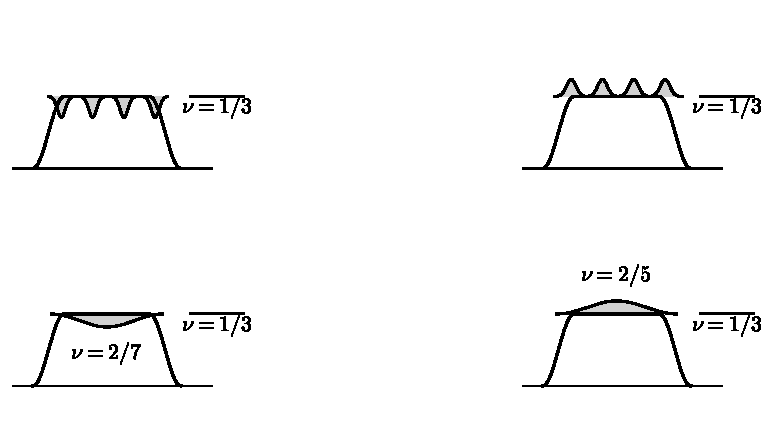
\includegraphics[width=0.72\textwidth]{fig_7.14.pdf}
\caption*{图 7.14\quad 分级 $\nu=2/7$ 与 $\nu=2/5$ 态。}
\end{figure}

\subsection{分级分数量子霍尔态——Laughlin 理论的推广}

\begin{keypoints}
\item 分级 FQH 态等价于准粒子的 Laughlin 态。
\end{keypoints}

要构造填充因子不是 $1/m$ 的更一般的 FQH 态，我们可以从 $\nu=1/m$ 的 Laughlin 态出发，加入准空穴或准粒子来改变平均电子密度。当其密度达到某一数值时，准空穴/准粒子气体自身也能形成一个 Laughlin 态。所得的态就是一个分级 FQH 态（见图 7.14）。

当 $\nu=1/3$ 态之上的电荷为 $e/3$ 的准空穴凝聚成一个 Laughlin 态时，我们得到 $\nu=2/7$ 的 FQH 态。波函数具有形式
\begin{align*}
&\Psi(z_1\cdots z_N)\\
&\quad=\int\prod_i\mathrm{d}^2\xi_i\;\prod(z_i-z_j)^3\,\mathrm{e}^{-\frac{1}{4l_B^2}\sum|z_i|^2}\prod(\xi_i-z_j)(\xi_i^*-\xi_j^*)^2\,\mathrm{e}^{-\frac{1}{4l_B^2}\frac{1}{3}|\xi_i|^2}
\end{align*}
当 $\nu=1/3$ 态之上的电荷为 $e/3$ 的准粒子凝聚成一个 Laughlin 态时，我们得到 $\nu=2/5$ 的 FQH 态。波函数为
\begin{equation*}
\Psi_c(z_i-z_N)=\int\prod_i\mathrm{d}^2\xi_i\;\prod_{i<j}(\xi_i-\xi_j)^2(\xi_i^*-2\partial_{z_i})\prod(z_i-z_j)^3\,\mathrm{e}^{-\frac{1}{4l_B^2}\sum|z_i|^2}
\end{equation*}
（译注：原书此式末尾的指数印作 $-\frac{1}{4l_B^2}|z_i|$，疑脱求和号与平方。）

我们可以用等离子体类比计算上述两个态的性质，但计算很复杂。下一节我们将推导 FQH 态的有效场论，并用有效理论计算上述分级 FQH 态的性质。有效场论大大简化了计算，我们能容易地得到 FQH 态的填充因子与准粒子的量子数。

\section{分数量子霍尔液体的有效理论}

\begin{keypoints}
\item FQH 态的低能有效理论是 $U(1)$ Chern--Simons 理论，它们捕捉 FQH 态的普适性质。
\end{keypoints}

我们已经见过几种不同的 FQH 态。一方面，这些 QH 态具有不同的分数电荷与不同的分数统计，这暗示不同的 FQH 态属于不同的量子相。另一方面，这些 FQH 态又都具有相同的对称性，我们无法用破缺的对称性来区分它们。实际上，FQH 态包含一种新型的序——拓扑序（见第 8 章）。我们需要用新的工具来刻画拓扑序。

系统研究拓扑序的一种途径是为 FQH 液体构造低能有效理论。有效理论能够捕捉 FQH 液体的普适性质，并为如何刻画和标记 FQH 液体中不同的拓扑序提供线索。下面我们将介绍一种构造有效理论的方法，它与 Haldane 和 Halperin 提出的分级构造密切相关（Haldane, 1983; Halperin, 1984）。

刻画 FQH 液体内部结构的首次尝试由 Girvin 和 MacDonald (1987) 提出，他们证明 Laughlin 态在一个非局域算符中具有非对角长程序。这一观察导致用 Ginzburg--Landau--Chern--Simons 有效理论来描述 FQH 液体（Read, 1989; Zhang et al., 1989）。这些进展产生了许多有趣而重要的结果，并加深了对 FQH 液体的理解。然而，这里我将尝试从更一般的观点出发描述 FQH 液体的内部结构。看来，FQH 液体的某些内部结构（特别是在所谓非阿贝尔 FQH 液体中的那些）无法用 Ginzburg--Landau--Chern--Simons 有效理论及相关的非对角长程序来描述。因此，我们需要发展更普遍的概念与表述，如拓扑序与拓扑场论，来描述 FQH 液体中的内部结构（见第 8 章）。在我看来，非对角长程序的概念并没有抓住 FQH 液体内部结构的本质。这里我们将不使用非对角长程序来发展有效理论（Blok and Wen, 1990a,b）。所得的有效理论只含纯 Chern--Simons 项。纯 Chern--Simons 形式更为紧凑，也更清楚地揭示分级 FQH 态的内部结构。

\subsection{Laughlin 态的有效理论}

\begin{keypoints}
\item FQH 液体的流体动力学与有效 Chern--Simons 理论。
\end{keypoints}

本节中我们只考虑单层自旋极化的 QH 系统。为构造分级态的有效理论，我们先设法得到 Laughlin 态的有效理论，然后在下一节用分级构造得到分级态的有效理论。

考虑磁场中的一个电子系统。为了涵盖更一般的情形，我们假设电子可以具有玻色统计或费米统计。系统的拉格朗日量具有如下形式（第一次量子化的版本）：
\begin{equation*}
\begin{aligned}
\mathcal{L}&=-eA^iJ^i+\text{动能/势能}\\
&=eA_iJ^i+\text{动能/势能}
\end{aligned}
\tag{7.3.1}
\end{equation*}
其中
\begin{equation*}
\pmb{J}(\pmb{x})=\sum_i\pmb{v}_i\delta(\pmb{x}-\pmb{x}_i),\qquad J^0(\pmb{x})=\sum_i\delta(\pmb{x}-\pmb{x}_i)
\tag{7.3.2}
\end{equation*}
分别是电子的流与密度，$(\pmb{x}_i,\pmb{v}_i)$ 是第 $i$ 个电子的位置与速度。动能/势能由 $\sum_i\frac{1}{2}mv_i^2+\sum_{i<j}V(\pmb{x}_i-\pmb{x}_j)$ 给出，其具体形式对我们并不重要。我们还假设了每个电子的电荷为 $-e$，光速为 $c=1$。

在流体动力学方法中，我们假设低能集体模式可以用密度与流 $J^\mu$ 描述，而低能有效理论具有形式 $\mathcal{L}(A_\mu,J^\nu)=eA_iJ^i+\mathcal{L}'(J^\mu)$。从 5.1.3 节与 5.3.3 节的讨论我们看到，有时一个态的低能激发可能太多，以至于无法用单一密度模式来描述。由于有能隙的 FQH 态的低能激发比超流体还要少，可以合理地假设单一密度模式足以描述 FQH 态的低能涨落。

在填充因子 $\nu=1/m$ 处（$m$ 对玻色型电子为偶整数，对费米型电子为奇整数），电子系统的基态由 Laughlin 波函数（Laughlin, 1983）给出：
\begin{equation*}
\Bigl[\prod(z_i-z_j)^m\Bigr]\mathrm{e}^{-\frac{1}{4l_B^2}\sum|z_i|^2}
\tag{7.3.3}
\end{equation*}
（这里我们已假设 $B<0$，于是 $(-e)B>0$。）为构造有效理论，我们注意到态 (7.3.3) 是不可压缩流体，其密度与磁场绑定，即 $J^0=(-e)\nu B/2\pi$。再结合有限的霍尔电导 $\sigma_{xy}=\frac{\nu e^2}{h}=\frac{\nu e^2}{2\pi\hbar}=\frac{\nu e^2}{2\pi}$，我们发现电子数流 $J^\mu$ 对电磁场的变化有如下响应：
\begin{equation*}
-e\delta J^\mu=-\sigma_{xy}\varepsilon^{\mu\nu\lambda}\partial_\nu\delta A_\lambda=-\frac{\nu e^2}{2\pi}\varepsilon^{\mu\nu\lambda}\partial_\nu\delta A_\lambda
\tag{7.3.4}
\end{equation*}
我们这样选择有效拉格朗日量 $\mathcal{L}(A_\mu,J^\nu)$，使它产生运动方程 (7.3.4)。为方便起见，引入一个 $U(1)$ 规范场 $a_\mu$ 来描述电子数流：
\begin{equation*}
J^\mu=\frac{1}{2\pi}\partial_\nu a_\lambda\varepsilon^{\mu\nu\lambda}
\end{equation*}
这样定义的流自动满足守恒定律。于是，产生式 (7.3.4) 的有效拉格朗日量取如下形式：
\begin{equation*}
\mathcal{L}=\Bigl[-m\frac{1}{4\pi}a_\mu\partial_\nu a_\lambda\varepsilon^{\mu\nu\lambda}+\frac{e}{2\pi}A_\mu\partial_\nu a_\lambda\varepsilon^{\mu\nu\lambda}\Bigr]
\tag{7.3.5}
\end{equation*}

式 (7.3.5) 只描述基态对外电磁场的线性响应。要对拓扑流体（例如 FQH 液体）有更完整的描述，我们需要把电子激发引入有效理论。特别是，我们要确保有效理论中包含一个携带与电子相同量子数的激发。

\subsection{有效理论中的电子与准粒子激发}

\begin{keypoints}
\item 单凭有效 Chern--Simons 理论并不是对 FQH 态的完整描述。为得到完整的有效理论，我们还需要指明电子算符。
\item 电子与准粒子/准空穴之间所要求的平凡互统计决定了准粒子与准空穴的量子数。
\end{keypoints}

让我们引入一个携带 $a_\mu$ 电荷 $l$ 的粒子。在有效理论 (7.3.5) 中，这样的粒子对应于如下源项：
\begin{equation*}
la_0\delta(\pmb{x}-\pmb{x}_0)
\tag{7.3.6}
\end{equation*}
该源项将产生一个电荷为
\begin{equation*}
Q=-le/m.
\tag{7.3.7}
\end{equation*}
的激发。这可以从运动方程 $\delta\mathcal{L}/\delta a_0=0$ 看出，由此方程得到
\begin{equation*}
J_0=\frac{1}{2\pi}\varepsilon_{ij}\partial_i a_j=-\frac{e}{2\pi m}B+\frac{l}{m}\delta(\pmb{x}-\pmb{x}_0)
\end{equation*}
右端第一项表明填充因子 $\nu\equiv 2\pi\frac{J_0}{-eB}$ 确实为 $\nu=1/m$，第二项则对应于与该激发相联系的电子密度的增加。

我们还看到，由源项 (7.3.6) 产生的激发带有 $l/m$ 个单位的 $a_\mu$ 通量。这样，如果有两个分别携带 $a_\mu$ 电荷 $l_1$ 与 $l_2$ 的激发，那么把一个激发绕另一个激发移动一周将诱导一个相位 $2\pi\times(a_\mu\text{-通量量子数})\times(a_\mu\text{ 电荷})$，\footnote{细心的读者可能注意到，这两个激发既带有 $a_\mu$ 电荷又带有 $a_\mu$ 通量。因此，把一个激发绕另一个激发移动一周所诱导的相位似乎应收到两项贡献：一项来自电荷绕通量运动，另一项来自通量绕电荷运动，如图 7.8 所描述的那样。这将给出相位 $2\pi\times\frac{l_1}{m}\times l_2+2\pi\times\frac{l_2}{m}\times l_1$，是式 (7.3.8) 中结果的两倍。然而，更仔细的计算表明，图 7.8 的图像并不适用于由 Chern--Simons 项诱导的电荷--通量束缚态。式 (7.3.8) 中的朴素结果恰好是正确的（见问题 7.3.1）。}即
\begin{equation*}
2\pi\times\frac{l_1}{m}\times l_2
\tag{7.3.8}
\end{equation*}
如果 $l_1=l_2\equiv l$，那么这两个激发是全同的。把它们互换将诱导式 (7.3.8) 中相位的一半，即
\begin{equation*}
\theta=\pi\frac{l^2}{m}
\tag{7.3.9}
\end{equation*}
这里的 $\theta$ 正是携带 $l$ 个单位 $a_\mu$ 电荷的激发的统计角。

我们的电子携带电荷 $-e$。从上面的讨论我们看到，电荷为 $-e$ 的激发对应于携带 $m$ 个单位 $a_\mu$ 电荷的粒子。这样的激发具有统计角 $\theta=\pi m$（见式 (7.3.9)）；因此，$m$ 为偶数时它是玻色子，$m$ 为奇数时它是费米子。于是，对玻色型电子取偶数 $m$ 的情形，以及对费米型电子取奇数 $m$ 的情形，我们可以把携带 $m$ 个单位 $a_\mu$ 电荷的激发认定为构成 FQH 液体的电子。具有电子的电荷与统计的激发的存在，支持了我们的 Chern--Simons 有效理论的正确性。

我们想强调，在有效理论中认定基本电子是非常重要的。正是这一认定，连同有效拉格朗日量，提供了对 FQH 液体拓扑性质的完整描述。我们将在下面看到，这一认定使我们能够确定准粒子激发的分数电荷与分数统计。

位置由复数 $\xi=x+\mathrm{i}y$ 描述的准空穴激发，是通过用 $\prod_i(\xi-z_i)$ 乘以基态波函数 (7.3.3) 产生的。注意到当一个电子绕准空穴一周时，波函数的相位改变 $2\pi$。这个 $2\pi$ 相位意味着电子与准空穴具有平凡的互统计。一般地，电子与一个允许的激发必须具有平凡的互统计，这样该激发的电子波函数才是单值的。

现在让我们试着通过插入一个携带 $l$ 个单位 $a_\mu$ 电荷的源项来产生激发。把一个电子绕这样的激发移动一周将诱导相位 $2\pi l$（见式 (7.3.8)）。电子波函数的单值性要求这样的相位是 $2\pi$ 的整数倍。因此 $a_\mu$ 电荷必须量子化为整数，也只有这些电荷对应的才是允许的激发。

从式 (7.3.7) 给出的激发电荷我们发现，$l=-1$ 对应于基本准空穴激发，而 $l=1$ 对应于基本准粒子激发。准粒子激发携带电荷 $-e/m$，准空穴携带电荷 $e/m$。从式 (7.3.9) 可见，二者都具有统计 $\theta=\pi/m$。我们看到，有效理论重现了 Laughlin 态中准粒子的著名结果（Arovas et al., 1984）。包含准粒子激发的完整有效理论为
\begin{equation*}
\begin{aligned}
\mathcal{L}&=\Bigl[-m\frac{1}{4\pi}a_\mu\partial_\nu a_\lambda\varepsilon^{\mu\nu\lambda}+\frac{e}{2\pi}A_\mu\partial_\nu a_\lambda\varepsilon^{\mu\nu\lambda}\Bigr]\\
&\quad+la_\mu j^\mu+\text{动能/势能}
\end{aligned}
\tag{7.3.10}
\end{equation*}
其中 $j^\mu$ 是准粒子的流，其形式由式 (7.3.2) 给出。式 (7.3.10) 连同对 $l$ 的量子化条件，是一个完整的低能有效理论，它捕捉了 $1/m$ Laughlin 态的拓扑性质。

\subsection*{问题 7.3.1}

证明式 (7.3.8)。（提示：可以从下面带两个激发的有效理论出发：
\begin{equation*}
\mathcal{L}=\Bigl[-\frac{1}{2}\frac{m}{2\pi}a_\mu\partial_\nu a_\lambda\varepsilon^{\mu\nu\lambda}+j^\mu a_\mu\Bigr]
\end{equation*}
其中 $j^\mu=j_1^\mu+j_2^\mu$，而
\begin{equation*}
\begin{aligned}
j_1^0(\pmb{x},t)&=l_1\delta(\pmb{x}-\pmb{x}_1(t)),&\qquad j_2^0(\pmb{x},t)&=l_2\delta(\pmb{x}-\pmb{x}_2(t)),\\
j_1^i(\pmb{x},t)&=l_1\dot{x}_1^i\delta(\pmb{x}-\pmb{x}_1(t)),&\qquad j_2^i(\pmb{x},t)&=l_2\dot{x}_2^i\delta(\pmb{x}-\pmb{x}_2(t)).
\end{aligned}
\end{equation*}
这里 $j^\mu$ 是两个激发的总流，$\pmb{x}_{1,2}(t)$ 是两个激发的位置。然后可以积掉 $a_\mu$，得到
\begin{equation*}
\int\mathrm{d}^3x\;\frac{1}{2}j^\mu\frac{1}{\frac{m}{2\pi}\partial_\lambda\epsilon^{\mu\lambda\nu}}j^\nu
\end{equation*}
交叉项可以写成
\begin{equation*}
\int\mathrm{d}^3x\;j_1^\mu\frac{1}{\frac{m}{2\pi}\partial_\lambda\epsilon^{\mu\lambda\nu}}j_2^\nu=\int\mathrm{d}^3x\;j_1^\mu f_\mu
\end{equation*}
其中 $f_\mu$ 满足
\begin{equation*}
\frac{m}{2\pi}\partial_\lambda\epsilon^{\mu\lambda\nu}f_\nu=j_2^\mu
\end{equation*}
假设 $\pmb{x}_2=\dot{\pmb{x}}_2=0$，即可求出 $f_i$。）

\subsection*{问题 7.3.2}

前面我们一直关注 Laughlin 态的拓扑性质。要对 Laughlin 态的动力学性质有所了解，我们需要在有效 Chern--Simons 理论中纳入如下的 Maxwell 项：
\begin{equation*}
\mathcal{L}=-m\frac{1}{4\pi}a_\mu\partial_\nu a_\lambda\varepsilon^{\mu\nu\lambda}+\frac{1}{2g_1}e^2-\frac{1}{2g_2}b^2
\tag{7.3.11}
\end{equation*}
其中 $e$ 与 $b$ 分别是 $a_\mu$ 的电场与磁场，且 $e_i=\dot{a}_i-\partial_i a^0$，$b=\partial_1a_2-\partial_2a_1$。求由 $e$ 与 $b$ 描述的集体涨落的运动方程。求集体激发的能隙。假设 $1/m$ Laughlin 态中的能隙为 $e^2/m^2 l_B$ 的量级，准空穴的尺寸为 $l_B$ 的量级。估计 $g_1$ 与 $g_2$ 的值。

\subsection{分级分数量子霍尔态的有效理论}

\begin{keypoints}
\item 不同的分级 FQH 态可以用一个整数 $K$ 矩阵和一个电荷矢量 $\pmb{q}$ 表征。
\item FQH 态的拓扑性质，如填充因子与准粒子量子数，可以容易地由 $K$ 矩阵和电荷矢量算出。
\item 不同的 $K$ 矩阵--电荷矢量对之间的等价关系。
\end{keypoints}

为得到分级 FQH 态的有效理论，让我们从费米型电子形成的 $1/m$ Laughlin 态出发。通过产生基本准粒子（记为 $l=1$）来增大填充因子。$l=1$ 的式 (7.3.10) 描述了存在这些准粒子时的 $1/m$ 态。现在出现两幅等价的图像。

\textbf{(a)}~在平均场理论方法中，我们可以把式 (7.3.10) 中的规范场 $a_\mu$ 视为固定背景，不允许 $a_\mu$ 对插入的源项 $j^\mu$ 作出响应。在这种情形下，准粒子气体的行为像"磁"场 $b=\partial_i a_j\varepsilon_{ij}$ 中的玻色子，这从式 (7.3.10) 的第二项可以看出。这些玻色子不携带任何电荷，因为准粒子数流 $j^\mu$ 不与电磁规范势 $A_\mu$ 直接耦合。当玻色子密度满足
\begin{equation*}
j^0=\frac{1}{p_2}\frac{b}{2\pi}
\end{equation*}
其中 $p_2$ 为偶数时，玻色子具有填充因子 $\frac{1}{p_2}$。玻色子的基态又可以用一个 Laughlin 态来描述。我们得到的最终电子态正是 Haldane (1983) 所构造的第二级分级 FQH 态。

\textbf{(b)}~如果我们让 $a_\mu$ 对 $j^\mu$ 的插入作出响应，那么准粒子将被 $a_\mu$ 通量缀饰。被缀饰的准粒子携带电荷 $-e/m$，统计为 $\theta=\pi/m$。当准粒子具有密度
\begin{equation*}
j^0=\frac{1}{(p_2-\frac{\theta}{\pi})}\frac{(-e)B}{2\pi m}
\end{equation*}
其中 $p_2$ 为偶数时，准粒子将具有填充因子 $\frac{1}{(p_2-\frac{\theta}{\pi})}$。这时，准粒子系统可以形成由波函数
\begin{equation*}
\prod_{i<j}(z_i-z_j)^{p_2-\frac{\theta}{\pi}}
\end{equation*}
描述的 Laughlin 态。用这种方法得到的最终电子态同样是一个第二级分级 FQH 态。这一构造由 Halperin (1984) 首先提出。(a) 与 (b) 两种构造给出同一个分级态，它们是等价的。

下面，我们将遵循 Haldane 的分级构造来推导分级 FQH 态的 Chern--Simons 有效理论（Blok and Wen, 1990a,b; Read, 1990; Fr\"{o}hlich and Kerler, 1991; Wen and Zee, 1992a）。注意到，在假设 (a) 之下，玻色子拉格朗日量（$l=1$ 时式 (7.3.10) 的第二项）正是把外电磁场 $eA_\mu$ 换成 $a_\mu$ 后的式 (7.3.1)。于是，我们可以重复从式 (7.3.3) 到式 (7.3.10) 的步骤，来构造玻色子 Laughlin 态的有效理论。引入一个新的 $U(1)$ 规范场 $\tilde{a}_\mu$ 来描述玻色子流，我们发现玻色子有效理论具有形式
\begin{equation*}
\mathcal{L}=-\frac{p_2}{4\pi}\tilde{a}_\mu\partial_\nu\tilde{a}_\lambda\varepsilon^{\mu\nu\lambda}+\frac{1}{2\pi}a_\mu\partial_\nu\tilde{a}_\lambda\varepsilon^{\mu\nu\lambda}
\tag{7.3.12}
\end{equation*}
在式 (7.3.12) 中，新的规范场 $\tilde{a}_\mu$ 描述玻色子的密度 $j^0$ 与流 $j^i$，它由
\begin{equation*}
j^\mu=\frac{1}{2\pi}\partial_\nu\tilde{a}_\lambda\varepsilon^{\mu\nu\lambda}
\end{equation*}
给出。这把 $a_\mu$ 与玻色子流 $a_\mu j^\mu$ 的耦合约化为 $a_\mu$ 与 $\tilde{a}_\mu$ 之间的一个 Chern--Simons 项（它成为式 (7.3.12) 中的第二项）。总的有效理论（包括原来的电子凝聚体）具有形式
\begin{equation*}
\begin{aligned}
\mathcal{L}&=\Bigl[-\frac{p_1}{4\pi}a_\mu\partial_\nu a_\lambda\varepsilon^{\mu\nu\lambda}+\frac{e}{2\pi}A_\mu\partial_\nu a_\lambda\varepsilon^{\mu\nu\lambda}\Bigr]\\
&\quad+\Bigl[-\frac{p_2}{4\pi}\tilde{a}_\mu\partial_\nu\tilde{a}_\lambda\varepsilon^{\mu\nu\lambda}+\frac{1}{2\pi}a_\mu\partial_\nu\tilde{a}_\lambda\varepsilon^{\mu\nu\lambda}\Bigr]
\end{aligned}
\tag{7.3.13}
\end{equation*}
其中 $p_1=m$ 是奇整数。式 (7.3.13) 就是第二级分级 FQH 态的有效理论。

% 块界说明：
% (1) 起点——书页 300（p315）以完整段落收束（"…where p1 = m is an odd integer.
%     Equation (7.3.13) is the effective theory of a second-level hierarchical FQH state."），
%     书页 301 顶部"有效理论可用于确定……"为新段落，故本块无 %--B-TAIL-- 区、正文不以 %JOIN% 起头。
% (2) 终点——书页 313（p328）末句止于 "These charged excitations carry integer charges and"，
%     其续文为 p329（书页 314）顶部 "are created by the electron operators Ψ†.
%     The above theory of edge excitations is formulated in terms of …"。
%     按约定该半句译文（"……携带整数电荷，并且"）留在本文件正文最末，未写入任何 TAIL 区；
%     ch7_d 请以 %JOIN% 起头续译"由电子算符 $\Psi^{\dagger}$ 所产生。……"，勿重复翻译本块已有内容。
% (3) 本块覆盖：7.3.3 后半（自书页 301 顶部起）、7.3.4（含表 7.1、7.2，问题 7.3.3–7.3.6）、
%     7.4 章节首与要点、7.4.1（图 7.15、7.16，脚注 47，问题 7.4.1–7.4.3）、7.4.2 至书页 313 末。
有效理论可以用来确定分级（hierarchical）FQH 态的物理性质。总填充因子由运动方程
$\delta\mathcal{L}/\delta a_{0}\allowbreak=\delta\mathcal{L}/\delta\tilde{a}_{0}\allowbreak=0$ 确定，其中
\begin{equation*}
-eB=p_{1}b-\tilde{b},\qquad b=p_{2}\tilde{b}
\end{equation*}
我们求得
\begin{equation*}
\nu=\frac{b}{-eB}=\frac{1}{p_{1}-\frac{1}{p_{2}}}. \tag{7.3.14}
\end{equation*}
通过引入 $(a_{1\mu},a_{2\mu})=(a_{\mu},\tilde{a}_{\mu})$，式 (7.3.13) 可以写成下面更紧凑的形式：
\begin{equation*}
\mathcal{L}=-\frac{1}{4\pi}K_{IJ}a_{I\mu}\partial_{\nu}a_{J\lambda}\varepsilon^{\mu\nu\lambda}
+\frac{e}{2\pi}q_{I}A_{\mu}\partial_{\nu}a_{I\lambda}\varepsilon^{\mu\nu\lambda} \tag{7.3.15}
\end{equation*}
其中 $K$ 是整数矩阵
\begin{equation*}
K=\begin{pmatrix} p_{1} & -1\\ -1 & p_{2} \end{pmatrix}
\end{equation*}
而 $\boldsymbol{q}$ 是整数矢量 $\boldsymbol{q}^{\top}=(q_{1},q_{2})=(1,0)$。这里 $\boldsymbol{q}$ 将被称为电荷矢量（charge vector）。填充因子 (7.3.14) 可以改写为 $\nu=\boldsymbol{q}^{\top}K^{-1}\boldsymbol{q}$。当 $(p_{1},p_{2})=(3,2)$ 时，该分级态对应于实验中观察到的 $\nu=2/5$ FQH 态。

第二级分级 FQH 态包含两种准粒子。一种是原来电子凝聚体中的准空穴（或涡旋），另一种是新玻色凝聚体中的准空穴（或涡旋）。这两种准空穴分别通过插入源项 $-j^{\mu}a_{\mu}$ 与 $-\tilde{j}^{\mu}\tilde{a}_{\mu}$ 来产生，其中 $\tilde{j}^{\mu}$ 与 $j^{\mu}$ 具有和式 (7.3.2) 类似的形式。第一种准空穴通过在电子波函数上乘以 $\prod_{i}(\xi-z_{i})$ 产生，而第二种准空穴则通过在玻色 Laughlin 波函数上乘以 $\prod_{i}(\eta-\xi_{i})$ 产生（这里 $\xi_{i}$ 是玻色子的复坐标，$\eta$ 是准空穴的位置）。

一个一般的准粒子由 $l_{1}$ 个第一种准粒子和 $l_{2}$ 个第二种准粒子组成，并由两个整数标记。这样的准粒子携带 $l_{1}$ 个单位的 $a_{1\mu}$ 荷和 $l_{2}$ 个单位的 $a_{2\mu}$ 荷，由下式描述
\begin{equation*}
(l_{1}a_{1\mu}+l_{2}a_{2\mu})j^{\mu} \tag{7.3.16}
\end{equation*}
积掉规范场之后，我们发现这样的准粒子携带 $\sum_{J}K_{IJ}l_{J}$ 个单位的 $a_{I\mu}$ 通量。因此，这样的准粒子的统计由下式给出
\begin{equation*}
\theta=\pi\pmb{l}^{\top}K^{-1}\pmb{l}
=\frac{1}{p_{2}p_{1}-1}\left(p_{2}l_{1}^{2}+p_{1}l_{2}^{2}+2l_{1}l_{2}\right)
\end{equation*}
而准粒子的电荷为
\begin{equation*}
Q_{q}=-e\boldsymbol{q}^{\top}K^{-1}\pmb{l}
=-e\frac{p_{2}l_{1}+l_{2}}{p_{2}p_{1}-1}
\end{equation*}
对于 $\nu=2/5$ 态（即 $(p_{1},p_{2})=(3,2)$），具有最小电荷的准粒子由 $(l_{1},l_{2})=(0,1)$ 标记。最小电荷为 $-e/5$。这样的准粒子具有统计 $\theta=\frac{3}{5}\pi$。

我们也可以构造更一般的 FQH 态。这些 FQH 态的有效理论仍具有式 (7.3.15) 给出的形式，只是现在指标 $I$ 从 1 取到某个整数 $n$（$n$ 将被称为该 FQH 态的级（level））。为了得到矩阵 $K$ 的形式，让我们假设在第 $n-1$ 级，有效理论由 $a_{I\mu}$（$I=1,\ldots,n-1$）以及 $K=K^{(n-1)}$ 的式 (7.3.15) 给出。准粒子携带 $a_{I\mu}$ 规范场的整数荷。现在考虑第 $n$ 级分级态，它通过具有 $a_{I\mu}$ 荷 $l_{I}|_{I=1,\ldots,n-1}$ 的准粒子的"凝聚"而得到。这个第 $n$ 级分级态的有效理论将由含 $n$ 个规范场的式 (7.3.15) 给出。第 $n$ 个规范场 $a_{n\mu}$ 来自新的凝聚体。矩阵 $K$ 由下式给出
\begin{equation*}
K^{(n)}=\begin{pmatrix} K^{(n-1)} & -\pmb{l}\\ -\pmb{l}^{\top} & p_{n} \end{pmatrix}
\end{equation*}
其中 $p_{n}$ 为偶数。电荷矢量 $\boldsymbol{q}$ 仍由 $(1,0,0,\ldots)$ 给出。通过迭代我们看到，广义分级态总是由整数对称矩阵描述，其中 $K_{II}$ 为偶数，唯独 $K_{11}$ 为奇数。新的凝聚体给出一种新的准粒子，它同样携带新规范场 $a_{n\mu}$ 的整数荷。因此，一个一般的准粒子总是携带 $a_{I\mu}$ 场的整数荷。

让我们用更一般的语言总结上述结果。我们知道，一个分级（或广义分级）FQH 态包含许多不同的凝聚体。这些凝聚体并不相互独立：一个凝聚体中的粒子对其他凝聚体中的粒子而言就像一根通量管（flux tube）。为了描述这种耦合，方便的做法是用 $U(1)$ 规范场来描述第 $I$ 个凝聚体的密度和流 $J_{I\mu}$：
\begin{equation*}
J_{I}^{\mu}=\frac{1}{2\pi}\varepsilon^{\mu\alpha\beta}\partial_{\alpha}a_{I\beta} \tag{7.3.17}
\end{equation*}
这时，不同凝聚体之间的耦合由规范场的 Chern--Simons 项描述：
\begin{equation*}
\mathcal{L}=-\frac{1}{4\pi}K_{IJ}a_{I\mu}\partial_{\nu}a_{J\lambda}\varepsilon^{\mu\nu\lambda}
+\frac{e}{2\pi}q_{I}A_{\mu}\partial_{\nu}a_{I\lambda}\varepsilon^{\mu\nu\lambda} \tag{7.3.18}
\end{equation*}
当 $K$ 取为一般的整数 $n\times n$ 矩阵，且 $K_{II}|_{I=1}$ 为奇数、$K_{II}|_{I>1}$ 为偶数、$\boldsymbol{q}^{\top}=(1,0,\ldots,0)$ 时，式 (7.3.18) 描述的是最一般的（阿贝尔）FQH 态 (Wen and Zee, 1992a)。填充因子由下式给出
\begin{equation*}
\nu=\boldsymbol{q}^{\top}K^{-1}\boldsymbol{q} \tag{7.3.19}
\end{equation*}
准粒子激发可以看作不同凝聚体中的涡旋。一个一般的准粒子由 $n$ 个整数 $l_{I}|_{I=1,..,n}$ 标记，并可由下面的源项产生：
\begin{equation*}
\mathcal{L}=l_{I}a_{I\mu}j^{\mu} \tag{7.3.20}
\end{equation*}
这样的准粒子将记作 $\psi_{\pmb{l}}$。式 (7.3.20) 中的 $j^{\mu}$ 具有如下形式
\begin{gather*}
\pmb{j}(x)=\dot{\pmb{x}}_{0}\delta(\pmb{x}-\pmb{x}_{0})\\
j^{0}(x)=\delta(\pmb{x}-\pmb{x}_{0}) \tag{7.3.21}
\end{gather*}
它在 $\pmb{x}_{0}$ 处产生一个准粒子。

当我们产生一个准粒子 $\psi_{\pmb{l}}$ 时，它会在所有凝聚体的密度中引起一个改变 $\delta J_{I}^{0}$。由式 (7.3.18) 与式 (7.3.20) 的运动方程，我们发现 $\delta J_{I}^{0}$ 满足
\begin{equation*}
\int\mathrm{d}^{2}x\,\delta J_{I}^{0}
=l_{J}(K^{-1})_{JI}\int\mathrm{d}^{2}x\,j^{0}=(\pmb{l}^{\top}K^{-1})_{I} \tag{7.3.22}
\end{equation*}
准粒子 $\psi_{\pmb{l}}$ 的电荷与统计由下式给出
\begin{equation*}
\theta_{\pmb{l}}=\pi\pmb{l}^{\top}K^{-1}\pmb{l},\qquad
Q_{\pmb{l}}=-e q_{I}\int\mathrm{d}^{2}x\,\delta J_{I}^{0}=-e\pmb{l}^{\top}K^{-1}\boldsymbol{q} \tag{7.3.23}
\end{equation*}
准粒子统计的这一结果来自如下观察：$2\pi\delta J_{I}^{0}$ 是 $a_{I\mu}$ 的通量，而准粒子携带 $l_{I}$ 个单位的 $a_{I\mu}$ 荷。

一个一般的电子激发可以看作一种特殊的（一般）准粒子，$\psi_{e}=\psi_{\pmb{l}_{e}}$，其中整数矢量 $\pmb{l}_{e}$ 由下式给出
\begin{equation*}
l_{eI}=K_{IJ}L_{J},\qquad L_{I}=\text{整数},\qquad q_{I}L_{I}=1 \tag{7.3.24}
\end{equation*}
我们可以证明，这些电子激发满足下列性质：它们携带单位电荷（见式 (7.3.23)）；它们具有费米统计；让一个电子激发 $\psi_{e}=\psi_{L}$ 绕任意准粒子激发 $\psi_{\pmb{l}}$ 一周，总是诱导 $2\pi$ 整数倍的相位；并且由式 (7.3.24) 定义的激发，就是满足上述三条性质的全部激发。

由式 (7.3.15) 的一般有效理论，我们发现广义分级态可以由一个整数值的 $K$ 矩阵和一个电荷矢量 $\boldsymbol{q}$ 来标记。现在我们想问这样一个问题：不同的 $(K,\boldsymbol{q})$ 是否描述不同的 FQH 态？注意到，通过对规范场 $a_{I\mu}$ 的重新定义，总可以把 $K$ 矩阵对角化成对角元为 $\pm1$ 的矩阵。这样看来，所有具有相同符号差（signature）的 $K$ 矩阵似乎都描述相同的 FQH 态，因为经过规范场的适当重新定义后，它们给出同一个有效理论。这个结论当然是错误的。我们想强调，仅凭有效拉格朗日量 (7.3.15) 并不能恰当描述分级态的内部序（或拓扑序）。正是有效拉格朗日量 (7.3.15) 连同 $a_{I\mu}$ 荷的量子化条件一起，才刻画了拓扑序。配备了允许 $U(1)$ 荷之量子化条件的 $U(1)$ 规范理论被称为紧致 $U(1)$ 理论。我们的有效理论 (7.3.15) 实际上是一个所有 $U(1)$ 荷都量子化为整数的紧致 $U(1)$ 理论。因此，允许的 $U(1)$ 荷构成一个 $n$ 维立方格子，我们将称之为电荷格子（charge lattice）。所以，当考虑两个不同 $K$ 矩阵的等价性时，只能使用保持电荷量子化条件不变（即保持电荷格子不变）的场重新定义。把电荷格子映到其自身的变换属于群 $SL(n,Z)$（行列式为 1 的整数矩阵群）：
\begin{equation*}
a_{I\mu}\rightarrow W_{IJ}a_{J\mu},\qquad W\in SL(n,Z) \tag{7.3.25}
\end{equation*}
由以上讨论我们看到，由 $(K_{1},\boldsymbol{q}_{1})$ 与 $(K_{2},\boldsymbol{q}_{2})$ 描述的两个 FQH 态是等价的（即它们属于同一个普适类（universality class）），如果存在 $W\in SL(n,Z)$ 使得
\begin{equation*}
\boldsymbol{q}_{2}=W\boldsymbol{q}_{1},\qquad K_{2}=WK_{1}W^{\top} \tag{7.3.26}
\end{equation*}
这是因为在变换 (7.3.25) 之下，由 $(K_{1},\boldsymbol{q}_{1})$ 描述的有效理论简单地变成由 $(K_{2},\boldsymbol{q}_{2})$ 描述的另一个有效理论。

我们想指出，在上述讨论中我们忽略了另一个拓扑量子数——自旋矢量（spin vector）。因此，式 (7.3.26) 的等价条件不适用于旋转不变系统。但是，式 (7.3.26) 确实适用于无序 FQH 系统，因为在无序系统中角动量不守恒，自旋矢量没有良好定义。关于自旋矢量的讨论可参见 Wen and Zee (1992c,d)。表 7.1 列出了一些常见的单层自旋极化 FQH 态的 $K$ 矩阵、电荷矢量 $\boldsymbol{q}$ 与自旋矢量 $\boldsymbol{s}$。

\subsection*{问题 7.3.3}
证明式 (7.3.24) 之下列出的四条性质。

\subsection{简单多层的分数量子霍尔态的有效理论}

\begin{keypoints}
\item $K$ 矩阵与多层 FQH 波函数。
\end{keypoints}

\begin{center}
\small 表 7.1\quad 某些简单的单层自旋极化 FQH 态的 $(K,\boldsymbol{q},\boldsymbol{s})$ 表达式\\[6pt]
\begin{tabular}{cccc}
\toprule
$\nu$ & $\boldsymbol{q}$ & $K$ & $\boldsymbol{s}$ \\
\midrule
$1/m$ & $(1)$ & $(m)$ & $\begin{pmatrix} m/2 \end{pmatrix}$ \\[10pt]
$1-1/m$ & $\begin{pmatrix}1\\0\end{pmatrix}$ &
$\begin{pmatrix}1 & 1\\ 1 & -(m-1)\end{pmatrix}$ &
$\begin{pmatrix}1/2\\ (1-m)/2\end{pmatrix}$ \\[18pt]
$2/5$ & $\begin{pmatrix}1\\0\end{pmatrix}$ &
$\begin{pmatrix}3 & -1\\ -1 & 2\end{pmatrix}$ &
$\begin{pmatrix}1/2\\ 1\end{pmatrix}$ \\[18pt]
$3/7$ & $\begin{pmatrix}1\\0\\0\end{pmatrix}$ &
$\begin{pmatrix}3 & -1 & 0\\ -1 & 2 & -1\\ 0 & -1 & 2\end{pmatrix}$ &
$\begin{pmatrix}1/2\\ 1\\ 1\end{pmatrix}$ \\
\bottomrule
\end{tabular}
\end{center}

到目前为止，我们只考虑了所谓的单层 FQH 态，其中二维电子气位于两种不同半导体的界面上。我们也可以制作具有多层界面的样品。置于强磁场之下时，不同层上的二维电子气可以形成多层 FQH 态。

用于构造分级态有效理论的同一方法，也可用来构造多层 FQH 态的有效理论。对多层 FQH 态而言，FQH 波函数与 $K$ 矩阵之间的联系变得非常透明。本节将集中讨论双层 FQH 态，不过推广到 $n$ 层 FQH 态是直截了当的。

我们想为下面这个简单的双层 FQH 态构造有效理论：
\begin{equation*}
\prod_{i<j}(z_{1i}-z_{1j})^{l}\prod_{i<j}(z_{2i}-z_{2j})^{m}\prod_{i,j}(z_{1i}-z_{2j})^{n}\,
\mathrm{e}^{-\frac{1}{4l_{B}^{2}}\left(\sum_{i}|z_{1i}|^{2}+\sum_{j}|z_{2j}|^{2}\right)}, \tag{7.3.27}
\end{equation*}
其中 $z_{Ii}$ 是第 $I$ 层中第 $i$ 个电子的复坐标。这里 $l$ 和 $m$ 是奇整数，使波函数与电子的费米统计相一致；$n$ 则可以是任意非负整数。上述波函数由 Halperin 首先提出，作为 Laughlin 波函数的推广 (Halperin, 1983)。这些波函数似乎能够解释双层 FQH 系统中观测到的部分主要 FQH 填充因子。

我们从第一层的单层 FQH 态出发，即 $\prod_{i<j}(z_{1i}-z_{1j})^{l}\mathrm{e}^{-\sum_{i}|z_{1i}|^{2}/4}$，它是一个 $1/l$ Laughlin 态，由如下有效理论描述
\begin{equation*}
\mathcal{L}=\left[-l\frac{1}{4\pi}a_{1\mu}\partial_{\nu}a_{1\lambda}\varepsilon^{\mu\nu\lambda}
+\frac{e}{2\pi}A_{\mu}\partial_{\nu}a_{\lambda}\varepsilon^{\mu\nu\lambda}\right] \tag{7.3.28}
\end{equation*}
其中 $a_{1\mu}$ 是描述第一层中电子密度和流的规范场。

考察式 (7.3.27) 的波函数可以看到，第二层中的一个电子束缚于第一层中的一个准空穴激发。这样的准空穴激发由 $n$ 个基本准空穴激发组成，并携带 $a_{1\mu}$ 荷 $-n$。一团准空穴由下面的有效理论描述：
\begin{equation*}
\mathcal{L}=-na_{1\mu}j^{\mu}+\text{动能/势能} \tag{7.3.29}
\end{equation*}
其中 $j^{\mu}$ 具有式 (7.3.2) 给出的形式。如前所述，在平均场理论中，如果忽略 $a_{1\mu}$ 场的响应，则式 (7.3.29) 简单地描述"磁场" $nb_{1}$ 中的一团玻色子，这里 $b_{1}=-\varepsilon_{ij}\partial_{i}a_{1j}$。现在我们想给式 (7.3.29) 中的每个准空穴附着一个（第二层中的）电子。这一操作有以下两个效果：由于电子携带电荷 $-e$，准空穴与电子的束缚态可以直接与电磁场 $A_{\mu}$ 耦合；并且束缚态表现得像一个费米子。束缚态的有效理论具有如下形式：
\begin{equation*}
\mathcal{L}=(eA_{\mu}-na_{1\mu})j^{\mu}+\text{动能/势能} \tag{7.3.30}
\end{equation*}
它现在（在平均场理论中）描述一团费米子。这些费米子感受到一个有效磁场 $-eB+nb_{1}$。

当第二层中的电子（即式 (7.3.30) 中的费米子）具有密度 $\frac{1}{m}(-eB+nb_{1})/2\pi$ 时（即它们具有有效填充因子 $1/m$），它们可以形成一个 $1/m$ Laughlin 态，对应于波函数中的 $\prod_{i<j}(z_{2i}-z_{2j})^{m}$ 部分。（注意这里 $eB<0$。）引入新规范场 $j^{\mu}=\frac{1}{2\pi}\partial_{\nu}a_{2\lambda}\varepsilon^{\mu\nu\lambda}$ 来描述式 (7.3.30) 中的费米子流 $j^{\mu}$，第二层中 $1/m$ 态的有效理论便具有形式
\begin{equation*}
\mathcal{L}=-m\frac{1}{4\pi}a_{2\mu}\partial_{\nu}a_{2\lambda}\varepsilon^{\mu\nu\lambda} \tag{7.3.31}
\end{equation*}
把式 (7.3.28)、式 (7.3.30) 与式 (7.3.31) 合在一起，我们就得到双层态的总有效理论，它具有式 (7.3.15) 给出的形式，其中 $K$ 矩阵与电荷矢量 $\boldsymbol{q}$ 由下式给出
\begin{equation*}
K=\begin{pmatrix} l & n\\ n & m \end{pmatrix},\qquad
\boldsymbol{q}=\begin{pmatrix}1\\1\end{pmatrix} \tag{7.3.32}
\end{equation*}
我们看到，$K$ 矩阵的矩阵元就是波函数中的幂次。该 FQH 态的填充因子仍由式 (7.3.19) 给出。

双层态中有两种（基本）准空穴激发。第一种通过在基态波函数上乘以 $\prod_{i}(\xi-z_{1i})$ 产生，第二种则由 $\prod(\xi-z_{2i})$ 产生。作为第一层与第二层这两个电子凝聚体中的涡旋，第一种准空穴由源项 $-a_{1\mu}j^{\mu}$ 产生，第二种准空穴由 $-a_{2\mu}j^{\mu}$ 产生。因此，双层态中一个一般的准粒子是若干第一类与第二类准空穴的束缚态，由式 (7.3.16) 描述。这些准粒子的量子数仍由式 (7.3.23) 给出。

\begin{center}
\small 表 7.2\quad 某些双层 FQH 态的 $(K,\boldsymbol{q},\boldsymbol{s})$ 表达式\\[6pt]
\begin{tabular}{cccc}
\toprule
$\nu$ & $\boldsymbol{q}$ & $K$ & $\boldsymbol{s}$ \\
\midrule
$1/m$ & $\begin{pmatrix}1\\1\end{pmatrix}$ &
$\begin{pmatrix}m & m\\ m & m\end{pmatrix}$ &
$\begin{pmatrix}m/2\\ m/2\end{pmatrix}$ \\[18pt]
$2/5$ & $\begin{pmatrix}1\\1\end{pmatrix}$ &
$\begin{pmatrix}3 & 2\\ 2 & 3\end{pmatrix}$ &
$\begin{pmatrix}3/2\\ 3/2\end{pmatrix}$ \\[18pt]
$1/2$ & $\begin{pmatrix}1\\1\end{pmatrix}$ &
$\begin{pmatrix}3 & 1\\ 1 & 3\end{pmatrix}$ &
$\begin{pmatrix}3/2\\ 3/2\end{pmatrix}$ \\[18pt]
$2/3$ & $\begin{pmatrix}1\\1\end{pmatrix}$ &
$\begin{pmatrix}3 & 0\\ 0 & 3\end{pmatrix}$ &
$\begin{pmatrix}3/2\\ 3/2\end{pmatrix}$ \\[18pt]
$2/3$ & $\begin{pmatrix}1\\1\end{pmatrix}$ &
$\begin{pmatrix}1 & 2\\ 2 & 1\end{pmatrix}$ &
$\begin{pmatrix}1/2\\ 1/2\end{pmatrix}$ \\
\bottomrule
\end{tabular}
\end{center}

一般地，(7.3.27) 类型的多层 FQH 态由一个矩阵元为整数、对角元为奇整数的 $K$ 矩阵描述。电荷矢量具有形式 $\boldsymbol{q}^{\top}=(1,1,\ldots,1)$。人们通常把双层 FQH 态 (7.3.27) 标记为 $(l,m,n)$。表 7.2 列出了一些简单双层态的 $K$ 矩阵、电荷矢量 $\boldsymbol{q}$ 与自旋矢量 $\boldsymbol{s}$。

由上述我们看到，(332) 双层态具有填充因子 2/5——这个填充因子也出现在单层分级态中。于是产生如下问题：双层 2/5 态与单层 2/5 态是否属于同一普适类？这个问题具有实验上的后果。我们可以设想这样的实验：从一个层间隧穿非常弱的系统中的 (332) 双层态出发，在保持填充因子不变的同时，把层间隧穿变得越来越强，双层态最终将变成单层 2/5 态。问题是：双层 (332) 态与单层 2/5 态之间的转变是平滑的渡越（crossover）还是相变？如果忽略自旋矢量，我们看到两个 2/5 态的 $K$ 矩阵和电荷矢量是等价的，因为它们通过一个 $SL(2,Z)$ 变换相联系。因此，在没有旋转对称性的情形下（此时自旋矢量没有良好定义），两个 2/5 态可以平滑地彼此转变。而当我们把自旋矢量包括进来时，两个 2/5 态并不等价，并且对旋转不变系统而言，它们被一个一级相变分隔开。

从表 7.2 我们还看到，存在两种不同的双层 2/3 态。当层内相互作用远强于层间相互作用时（真实样品中正是这种情形），基态波函数倾向于让同层电子之间具有更高阶的零点。因此，(330) 态的能量应当比 (112) 态低。单层 2/3 态的 $K$ 矩阵和电荷矢量与 (112) 态的等价，而与 (330) 态的不等价。因此，要把一个双层 2/3 态（即 (330) 态）变成单层 2/3 态，无论旋转对称性如何都必须经过一次相变。

双层 (mmm) 态是一个有趣的态，因为 $\det K=0$。Fertig (1989)、Brey (1990) 与 MacDonald 等 (1990) 研究了 (111) 态，发现了一个无能隙的集体模式。Wen 和 Zee (1992b) 研究了更一般的 (mmm) 态，并指出 (mmm) 态（在无层间隧穿时）自发破缺一个 $U(1)$ 对称性，是一种中性超流体。更详细的讨论（包括其实验含义）可参见 Wen and Zee (1993)、Murphy et al. (1994) 与 Yang et al. (1994)。

\subsection*{问题 7.3.4}
让我们首先忽略自旋矢量 $\boldsymbol{s}$。证明表 7.1 中单层 2/5 态的 $(K,\boldsymbol{q})$ 与表 7.2 中双层 2/5 态的 $(K,\boldsymbol{q})$ 等价。再证明，这两个态的 $(K,\boldsymbol{q},\boldsymbol{s})$ 却不等价。（在存在自旋矢量 $\boldsymbol{s}$ 时，等价关系变为 $\boldsymbol{s}_{2}=W\boldsymbol{s}_{1}$、$\boldsymbol{q}_{2}=W\boldsymbol{q}_{1}$ 与 $K_{2}=WK_{1}W^{+}$。）

\subsection*{问题 7.3.5}
考虑双层 (lmn) 态 (7.2.6)。利用有效理论 (7.3.15) 与式 (7.3.32) 求出填充因子。并求出第一层与第二层中准空穴的分数电荷与分数统计。（可以把结果与问题 7.2.5 的结果比较。）

\subsection*{问题 7.3.6}
假设双层 (mmm) 态的有效理论具有形式
\begin{equation*}
\mathcal{L}=-\frac{1}{4\pi}K_{IJ}a_{I\mu}\partial_{\nu}a_{J\lambda}\varepsilon^{\mu\nu\lambda}
+\frac{1}{2g_{1}}\pmb{e}_{I}\cdot\pmb{e}_{I}-\frac{1}{2g_{2}}b_{I}b_{I}
\end{equation*}
其中 $\pmb{e}_{I}$ 与 $b_{I}$ 分别是 $a_{I\mu}$ 的"电场"与"磁场"。
\begin{enumerate}
\item 证明 (mmm) 态正如超流体一样具有无能隙激发。求出无能隙激发的速度。
\item 同样像超流体一样，(mmm) 态包含能量为 $\gamma\ln L$ 的涡旋激发，这里 $L$ 是系统的线度。求出能量最小的涡旋的 $\gamma$ 值。（提示：在 (mmm) 态中，$l_{I}$ 的 $a_{I\mu}$ 荷仍量子化为整数。）
\item 如果我们确实把 (mmm) 态当作超流体，你能辨认出破缺的对称性和序参量吗？
\end{enumerate}

\section{分数量子霍尔液体中的边缘激发}

\begin{keypoints}
\item FQH 态\emph{总是}具有无能隙的边缘激发。
\item FQH 态的边缘激发构成手征 Luttinger 液体。
\item 边缘激发的结构由体拓扑序决定。
\end{keypoints}

由于电子之间排斥性的相互作用和强关联，尽管第一朗道能级只是部分填充，QH 液体仍是一个不可压缩态。QH 态中的所有体激发都具有有限的能隙。QH 态与绝缘体非常相似：两者都具有有限能隙和短程的电子传播子。正是由于这种相似性，人们曾对如下事实感到困惑：QH 系统的输运性质显然与普通绝缘体截然不同。Halperin 首先指出，IQH 态含有无能隙的边缘激发 (Halperin, 1982)。IQH 态的非平庸输运性质正来自这些无能隙边缘激发 (Halperin, 1982; Trugman, 1983; MacDonald and Streda, 1984; Streda et al., 1987; Buttiker, 1988; Jain and Kivelson, 1988a,b)。例如，对一个 IQH 样品做两端测量，只有当源与汇通过边缘连通时才可能给出有限电阻。如果源与汇不被任何边缘连通，那么两端测量在零温下将给出无穷大电阻——这是一个与绝缘体十分相似的结果。Halperin 还研究了 IQH 态边缘激发的动力学性质，发现边缘激发由一个手征的一维费米液体理论描述。

鉴于 FQH 态与 IQH 态输运性质的相似性，一个自然的猜想是：FQH 态的输运同样由边缘激发支配 (Beenakker, 1990; MacDonald, 1990)。然而，由于 FQH 态本质上是多体态，FQH 态中的边缘激发无法通过填充单粒子能级来构造。换言之，FQH 态的边缘激发不应当用费米液体来描述。因此，我们需要一种全新的方法来理解 FQH 液体边缘态的动力学性质 (Wen, 1992, 1995)。

在下一节中，我们将用费米液体理论研究 $\nu=1$ IQH 态的边缘激发。然后，我们将利用流代数（或玻色化，见 Tomonaga, 1950; Luttinger, 1963; Coleman, 1975）来建立 FQH 态边缘激发的理论。

\subsection{整数量子霍尔边缘态的费米液体理论}

\begin{keypoints}
\item IQH 液体的基态通过填充单粒子能级得到。因此，低能边缘激发可以通过以略有不同的方式填充这些单粒子能级来获得。
\end{keypoints}

考虑均匀磁场 $B$ 中的一团无相互作用电子气。在对称规范下，角动量是一个好量子数。能量与动量的共同本征态构成一个环状分布（见图 7.10）。因此，在光滑的圆形势 $V(r)$ 存在时，单粒子能级如图 7.15 所示。基态通过填充能量最低的 $N$ 个能级得到。这样的态对应于一个具有均匀密度的圆形液滴（见图 7.11）。

\begin{figure}[H]
\centering
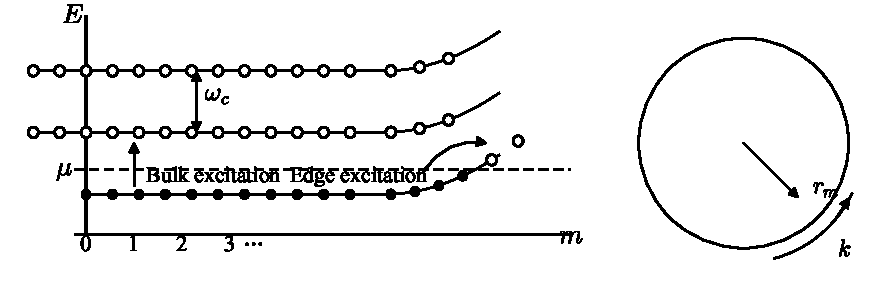
\includegraphics[width=0.72\textwidth]{fig_7.15.pdf}
\caption*{图 7.15\quad 光滑势 $V(r)$ 存在时头三个朗道能级中的能级。这里 $m$ 是能级的角动量。化学势 $\mu$ 以下的能级各被一个电子占据，从而给出 IQH 态。改变边缘附近的占据数，便产生 IQH 态的无能隙边缘激发。}
\end{figure}

在零朗道能级中，角动量 $m$ 的态的能量为
\begin{equation*}
E_{m}=\frac{1}{2}\hbar\omega_{c}+V(r_{m})
\end{equation*}
其中 $r_{m}=\sqrt{2m}\,l_{B}$ 是 $m$ 态的半径。从图 7.15 我们看到，体激发具有有限的能隙 $\hbar\omega_{c}$。边缘激发可以这样产生：把一个电子从边缘附近的 $m$ 态移到 $m+1$ 态（见图 7.15）。由于在热力学极限 $r_{m}\to\infty$ 下 $r_{m+1}-r_{m}\to0$，边缘激发是无能隙的。

由于 $m$ 态具有半径 $r_{m}$，我们也可以把角动量 $m$ 看作沿边缘的动量 $k=m/r_{m}$。这使我们能够把 $E_{m}$ 当作一个能量--动量关系
\begin{equation*}
E(k)=\frac{1}{2}\hbar\omega_{c}+V(2l_{B}^{2}k)
\end{equation*}
用 $E(k)$ 来表示，我们的电子系统可以用一个无相互作用的哈密顿量描述：
\begin{equation*}
H=\sum_{k}E(k)c_{k}^{\dagger}c_{k} \tag{7.4.1}
\end{equation*}
上述哈密顿量描述一个一维手征费米液体（chiral Fermi liquid）。我们称它为手征费米液体，是因为它只有一个费米点，并且所有低能激发都朝同一个方向传播。\footnote{相比之下，通常的一维费米液体有两个费米点，同时包含左移与右移两种成分。}我们由此得出结论：$\nu=1$ IQH 态的边缘激发由一维手征费米液体 (7.4.1) 描述。

\begin{figure}[H]
\centering
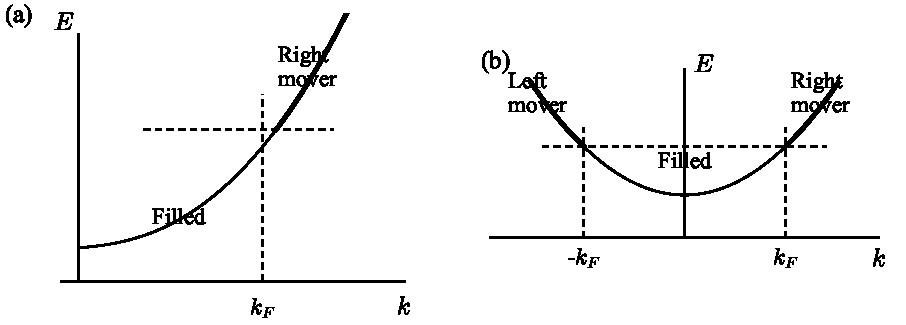
\includegraphics[width=0.72\textwidth]{fig_7.16.pdf}
\caption*{图 7.16\quad (a) 能量--角动量关系 $E_{m}$ 可以看作能量--动量关系 $E(k)$。边缘激发可以看作一维手征费米液体的激发，其中只含右移成分。(b) 通常的一维费米液体的色散关系同时包含右移与左移成分。}
\end{figure}

\subsection*{问题 7.4.1}
证明 IQH 边缘激发的速度 $v=\partial E(k)/\partial k$ 由 $cE/B$ 给出，其中 $c$ 是光速，$E=-\partial V(r)/\partial r$ 是约束势 $V(r)$ 在边缘处产生的电场。设 $\nu=1$ IQH 液滴包含 $N$ 个电子，求出手征费米液体的费米动量 $k_{F}$。

\subsection*{问题 7.4.2}
一个 $\nu=1$ IQH 态被圆形光滑势 $V(r)$ 约束，包含 $N$ 个电子。求出基态的总角动量 $M_{0}$。求出总角动量为 $M_{0}+m$ 的低能粒子--空穴激发的数目，其中 $m=-1$ 及 $m=1,2,3,4,5$。证明在热力学极限下，具有相同总角动量的激发具有相同的能量。

\subsection*{问题 7.4.3}
考虑一个由 $H=\sum_{k}(v_{1}k\,c_{1,k}^{\dagger}c_{1,k}+v_{2}k\,c_{2,k}^{\dagger}c_{2,k})$ 描述的一维无相互作用费米子系统。混合项 $\sum_{k}(\gamma c_{1,k}^{\dagger}c_{2,k}+\text{h.c.})$ 是一个相关微扰。证明：当系统同时具有右移与左移成分（即 $v_{1}v_{2}<0$）时，这个相关微扰会打开一个有限的能隙，并剧烈地改变系统的低能性质。然而，对于所有激发都朝同一方向运动的手征费米液体（即 $v_{1}v_{2}>0$），这个相关微扰不诱导任何能隙。事实上，我们认为任何微扰都无法在一维手征费米液体中诱导出能隙。一维手征费米液体中的无能隙激发对所有微扰都是稳健的，并且在拓扑上是稳定的。

\subsection{流体动力学方法——$1/m$ Laughlin 态}

\begin{keypoints}
\item 边缘激发来自流代数（Kac--Moody 代数）。
\item 无法通过填充单粒子能级来构造 FQH 边缘激发。
\end{keypoints}

由于 $1/m$ Laughlin FQH 态不能通过填充单粒子能级得到，我们不能用上一节的图像来构造 $1/m$ Laughlin 态的边缘激发。由于不知道如何从相互作用电子的哈密顿量导出 FQH 边缘理论，下面我们转而尝试猜测一个低能有效理论。

猜测边缘激发动力学理论的最简单方法是使用流体动力学方法。在这种方法中，人们利用这样一个事实：FQH 态是不可压缩、无旋的液体，不含低能体激发。因此，唯一的低能激发（在体能隙之下）是 FQH 液滴形变产生的表面波。这些表面波被认定为 FQH 态的边缘激发。

在流体动力学方法 (Wen, 1992) 中，我们首先研究 FQH 液滴上表面波的经典理论，然后把经典理论量子化，得到边缘激发的量子描述。令人惊叹的是，由经典理论得到的这个简单的量子描述，在低能下给出了边缘激发的完整描述，并使我们能够计算沿边缘的电子与准粒子传播子。

考虑一个填充因子为 $\nu$、被势阱约束的 FQH 液滴。由于电导非零，势阱的电场产生一个沿边缘流动的持续电流：
\begin{equation*}
\pmb{j}=\sigma_{xy}\hat{z}\times\pmb{E},\qquad \sigma_{xy}=\nu\frac{e^{2}}{h}
\end{equation*}
这意味着边缘附近的电子以速度
\begin{equation*}
v=\frac{E}{B}c
\end{equation*}
沿边缘漂移，这里 $c$ 是光速。于是，边缘波（边缘的形变）也以速度 $v$ 传播。让我们用一维密度 $\rho(x)=nh(x)$ 来描述边缘波，其中 $h(x)$ 是边缘的位移，$x$ 是沿边缘的坐标，而 $n=\nu/2\pi l_{B}^{2}$ 是体内的二维电子密度。（这里 $l_{B}=\sqrt{c/eB}$ 是磁长度。）我们看到，边缘波的传播由下面的波动方程描述：
\begin{equation*}
\partial_{t}\rho+v\partial_{x}\rho=0 \tag{7.4.2}
\end{equation*}
注意，边缘波总是朝一个方向传播；不存在朝相反方向传播的波。

边缘波的哈密顿量（即能量）由下式给出
\begin{equation*}
H=\int\mathrm{d}x\,\frac{1}{2}e\rho E h=\int\mathrm{d}x\,\pi\frac{v}{\nu}\rho^{2} \tag{7.4.3}
\end{equation*}
其中我们用到了 $h=\rho/n=\rho\frac{2\pi c}{eB}$。在动量空间中，式 (7.4.2) 与式 (7.4.3) 可以改写为
\begin{equation*}
\dot{\rho}_{k}=-\mathrm{i}vk\rho_{k},\qquad
H=2\pi\frac{v}{\nu}\sum_{k>0}\rho_{-k}\rho_{k} \tag{7.4.4}
\end{equation*}
其中 $\rho_{k}=\int\mathrm{d}x\,\frac{1}{\sqrt{L}}\mathrm{e}^{\mathrm{i}kx}\rho(x)$，而 $L$ 是边缘的长度。我们发现，如果把 $\rho_{k}|_{k>0}$ 认作"坐标"，并把 $\pi_{k}=\mathrm{i}2\pi\rho_{-k}/\nu k$ 认作相应的正则"动量"，那么标准哈密顿方程
\begin{equation*}
\dot{q}=\frac{\partial H}{\partial p},\qquad \dot{p}=-\frac{\partial H}{\partial q}
\end{equation*}
将重现运动方程 $\dot{\rho}_{k}=\mathrm{i}vk\rho_{k}$。这使我们得以认定正则"坐标"与"动量"。有趣的是，位移 $h(x)$ 同时包含"坐标"与"动量"。这是边缘波的手征性质所致。

知道了正则坐标与动量之后，量子化经典理论就很容易了。我们只需把 $\rho_{k}$ 和 $\pi_{k}$ 看作满足 $[\rho_{k},\pi_{k'}]=\mathrm{i}\delta_{kk'}$ 的算符。于是，量子化之后我们得到
\begin{align*}
[\rho_{k},\rho_{k'}]&=\frac{\nu}{2\pi}k\delta_{k+k'},\qquad
k,k'=\text{整数}\times\frac{2\pi}{L} \tag{7.4.5}\\
H&=2\pi\frac{v}{\nu}\sum_{k>0}\rho_{-k}\rho_{k}
\end{align*}
上述代数称为 (U(1)) Kac--Moody（K--M）代数 (Kac, 1983; Goddard and Olive, 1985, 1986)。类似的代数也曾出现在 Tomonaga 模型中 (Tomonaga, 1950; Luttinger, 1963; Coleman, 1975)。注意，式 (7.4.5) 简单地描述了一组退耦谐振子（由 $(\rho_{k},\rho_{-k})$ 生成）。因此，式 (7.4.5) 是一个一维自由声子理论（只有单一分支）。对于 $k>0$，$\rho_{k}^{\dagger}=\rho_{-k}$ 产生一个动量为 $k$、能量为 $vk$ 的声子，而 $\rho_{k}$ 湮灭一个声子。式 (7.4.5) 为 Laughlin 态的低能边缘激发提供了完整的描述。

这里考虑的边缘激发不改变系统的总电荷，因而是中性的。下面我们将讨论带电激发，并由 K--M 代数 (7.4.5) 计算电子传播子。

低能电荷激发显然对应于把电子加到边缘上（从边缘移走）。这些带电激发携带整数电荷，并且
由电子算符 $\Psi^\dagger$ 产生。上述边缘激发理论是用一维密度算符 $\rho(x)$ 来表述的。因此，中心任务是把电子算符用密度算符表示出来。边缘上的电子算符产生一个局域电荷，故应满足
\begin{equation*}
[\rho(x),\Psi^\dagger(x')]=\delta(x-x')\Psi^\dagger(x')
\tag{7.4.6}
\end{equation*}
由于 $\rho$ 满足 K--M 代数 (7.4.5)，可以证明
\begin{equation*}
[\rho(x_1),\rho(x_2)]=\mathrm{i}\frac{\nu}{2\pi}\delta'(x_1-x_2)
\end{equation*}
或者
\begin{equation*}
[\rho(x_1),\phi(x_2)]=-\mathrm{i}\nu\delta(x_1-x_2)
\end{equation*}
其中 $\phi$ 由 $\rho=\frac{1}{2\pi}\partial_x\phi$ 给出。我们看到，$\rho(x)$ 可以视为 $\phi$ 的泛函导数，即 $\rho(x)=-\mathrm{i}\nu\frac{\delta}{\delta\phi(x)}$。利用这一关系，可以证明满足式 (7.4.6) 的算符由下式给出（Wen, 1992）：
\begin{equation*}
\Psi\propto\mathrm{e}^{\mathrm{i}\frac{1}{\nu}\phi}
\tag{7.4.7}
\end{equation*}

式 (7.4.6) 只表明算符 $\Psi$ 携带电荷 $e$。为了把 $\Psi$ 认作电子算符，我们还需要证明 $\Psi$ 是费米性算符。利用 K--M 代数 (7.4.5)，我们发现（见问题 7.4.8）
\begin{equation*}
\Psi(x)\Psi(x')=(-)^{1/\nu}\Psi(x')\Psi(x)
\tag{7.4.8}
\end{equation*}

我们看到，式 (7.4.7) 中的电子算符 $\Psi$ 只有当 $1/\nu=m$ 为奇整数时才是费米性的，此时该 FQH 态是一个 Laughlin 态。

在上述讨论中，我们做了一个并不普遍成立的假设。我们假设了不可压缩 FQH 液体只包含\emph{一种}不可压缩流体组分，从而只导致一支边缘激发。上述结果意味着，当 $\nu\neq1/m$ 时，只有一支的边缘理论不包含电子算符，因而是不自洽的。我们的单支边缘理论只适用于 $\nu=1/m$ 的 Laughlin 态。

现在让我们计算 $\nu=1/m$ Laughlin 态边缘上的电子传播子。由于 $\phi$ 是一个自由声子场，其传播子为
\begin{equation*}
\langle\phi(x,t)\phi(0)\rangle=-\nu\ln(x-vt)+\text{常数}
\end{equation*}
电子传播子可以容易地算出为
\begin{equation*}
G(x,t)=\langle T(\Psi^\dagger(x,t)\Psi(0))\rangle=\exp[\frac{1}{\nu^2}\langle\phi(x,t)\phi(0)\rangle]\propto\frac{1}{(x-vt)^m}
\tag{7.4.9}
\end{equation*}

我们看到的第一件事是：FQH 态边缘上的电子传播子获得了一个不等于 1 的非平庸指数 $m=1/\nu$。这意味着 FQH 态边缘上的电子是强关联的，不能用费米液体理论来描述。我们将把这类电子态称为手征 Luttinger 液体（chiral Luttinger liquid）。

我们想强调，指数 $m$ 是量子化的。指数的量子化与下述事实直接相关：该指数与电子的统计性质联系在一起（见式 (7.4.8)）。因此，该指数是一个拓扑数，与电子相互作用、边缘势等无关。尽管该指数是边缘态的性质，改变它的唯一途径却是通过体态中的相变。因此，这个指数可以看作一个表征\emph{体内} FQH 态拓扑序的量子数。

在动量空间中，电子传播子具有形式
\begin{equation*}
G(k,\omega)\propto\frac{(vk+\omega)^{m-1}}{\omega-vk+\mathrm{i}0^+\operatorname{sgn}(\omega)}
\end{equation*}
这个反常指数 $m$ 可以在隧穿实验中测量。由 $\operatorname{Im}G$ 可得，电子的隧穿态密度为
\begin{equation*}
N(\omega)\propto|\omega|^{m-1}
\end{equation*}
这表明，对金属--绝缘体--FQH 结，微分电导具有 $\frac{\mathrm{d}I}{\mathrm{d}V}\propto V^{m-1}$ 的形式。

\subsection*{问题 7.4.4}

证明式 (7.4.8)。（提示：先证明 $[\phi(x),\phi(y)]=\frac{\pi}{q}\operatorname{sgn}(x-y)$；译注：原文之 $q$ 疑为 $\nu$ 之误。）

\subsection*{问题 7.4.5}

\textbf{玻色化与费米化（bosonization and fermionization）}当 $m=1$ 时，本节的讨论意味着 $\nu=1$ 的 IQH 边缘态可以用自由声子理论
\begin{equation*}
H_b=2\pi v\sum_{k>0}\rho_k^\dagger\rho_k
\end{equation*}
来描述。在 7.4.1 节中，我们发现 $\nu=1$ 的 IQH 边缘态可以用自由手征费米子模型
\begin{equation*}
H_f=\sum_k vk:c_k^\dagger c_k:=\sum_{k>0}vkc_k^\dagger c_k-\sum_{k<0}vkc_kc_k^\dagger
\end{equation*}
来描述。正规排序定义为：当 $k>0$ 时 $:c_k^\dagger c_k:=c_k^\dagger c_k$；当 $k<0$ 时 $:c_k^\dagger c_k:=-c_kc_k^\dagger$。在本问题中，我们将研究这两种描述之间的直接关系。从费米子描述切换到玻色子描述称为玻色化，从玻色子描述切换到费米子描述称为费米化。
\begin{enumerate}
\item 求玻色模型前五个能级的能量及其简并度。将你的结果与问题 7.4.2 的结果作比较。
\item 令 $\rho_f(x)=:c^\dagger(x)c(x):$。在 $k$ 空间中，$\rho_{f,k}=\sum_q{}^{\prime}:c_q^\dagger c_{q+k}:$，其中求和 $\sum_q{}^{\prime}$ 限制在使 $c_{q+k}$ 与 $c_q$ 的动量都处于 $[-\Lambda,+\Lambda]$ 范围之内的那些项。正规排序后的 $\rho_f(x)$ 在基态中的平均值为零，这与玻色理论中的 $\rho$ 一致。证明 $\rho_{f,k}$ 满足与 $\rho_k$ 相同的 K--M 代数（见式 (7.4.5)，取 $\nu=1$）。（提示：对大的正 $k$ 有 $c_k^\dagger c_k=0$，对大的负 $k$ 也有 $c_k^\dagger c_k=0$。）
\item 证明 $H_f=2\pi v\sum_{k>0}\rho_{f,k}^\dagger\rho_{f,k}$。
\end{enumerate}

\subsection{边缘激发的微观理论}

\begin{keypoints}
\item K--M 代数与 Laughlin 波函数之间的关系。
\item 由等离子体类比得到的电子等时关联。
\end{keypoints}

在这一节中，我们将给出 Laughlin 态边缘激发的一个微观理论。具体起见，让我们考虑第一朗道能级中的电子气体。我们假设电子由理想哈密顿量 (7.2.5) 描述。$\nu=1/3$ 的 Laughlin 波函数
\begin{equation*}
\Psi_3(z_i)=Z^{-1/2}\prod_{i<j}(z_i-z_j)^3\prod_k\mathrm{e}^{-|z_k|^2/4l_B^2}
\tag{7.4.10}
\end{equation*}
具有零能量\footnote{这里，为方便起见，我们把能量零点移到了第零朗道能级。}，并且是理想哈密顿量的一个精确基态。（译注：原书指数中印作 $4l_B$，应为 $4l_B^2$。）在这一节中，我们将假设磁长度 $l_B=1$。式 (7.4.10) 中的 $Z$ 是归一化因子。然而，Laughlin 态 (7.4.10) 并不是唯一的零能量态。容易检验，下列类型的态都具有零能量：
\begin{equation*}
\Psi(z_i)=P(z_i)\Psi_3(z_i)
\tag{7.4.11}
\end{equation*}
其中 $P(z_i)$ 是 $z_i$ 的对称多项式。事实上，反之亦然：所有零能态都具有 (7.4.11) 的形式。这是因为，要使一个费米子态具有零能量，当任意两个电子 $i$ 与 $j$ 相互靠拢时，$\Psi$ 必须至少以 $(z_i-z_j)^3$ 的快慢消失（$(z_i-z_j)^2$ 的可能性被费米统计所排除）。由于 Laughlin 波函数只在 $z_i=z_j$ 时为零，故 $P=\Psi/\Psi_3$ 是一个有限函数。由于 $\Psi$ 与 $\Psi_3$ 都是第一朗道能级中的反对称函数，$P$ 是一个对称的全纯函数，因而只能是一个对称多项式。

在式 (7.4.11) 的所有态中，Laughlin 态描述半径最小的一个圆形液滴。所有其他的态都是 Laughlin 态液滴的形变和/或膨胀。因此，由 $P$ 生成的态对应于 Laughlin 态的边缘激发。

首先，让我们考虑零能空间（即对称多项式的空间）。我们知道，对称多项式的空间由多项式 $s_n=\sum_iz_i^n$（通过乘法与加法）生成。令 $M_0=3\frac{N(N-1)}{2}$ 为 Laughlin 态 (7.4.10) 的总角动量，则态 $\Psi$ 将具有角动量 $M=\Delta M+M_0$，其中 $\Delta M$ 是对称多项式 $P$ 的次数。由于我们只有一个零次对称多项式和一个一次对称多项式，即 $s_0=1$ 与 $s_1=\sum_iz_i$，故 $\Delta M=0,1$ 的零能态是非简并的。然而，当 $\Delta M=2$ 时，我们有两个由 $P=s_2$ 与 $P=s_1^2$ 生成的零能态。对一般的 $\Delta M$，零能态的简并度由下式给出：
\begin{equation*}
\begin{array}{cccccccc}
\Delta M: & 0 & 1 & 2 & 3 & 4 & 5 & 6\\
\text{简并度}: & 1 & 1 & 2 & 3 & 5 & 7 & 11
\end{array}
\tag{7.4.12}
\end{equation*}

这里我们想指出，式 (7.4.12) 中的简并度正是我们从宏观理论所预期的。我们知道，对于圆形液滴，角动量 $\Delta M$ 可以视为沿边缘的动量 $k=2\pi\Delta M/L$，其中 $L$ 是 FQH 液滴的周长。按照宏观理论，（中性的）边缘激发由密度算符 $\rho_k$ 生成。容易检验，由密度算符生成的边缘态对每一个 $\Delta M$ 都具有与式 (7.4.12) 相同的简并度。例如，$\Delta M=2$ 的两个态由 $\rho_{\kappa_0}^2$ 与 $\rho_{2\kappa_0}$ 生成，其中 $\kappa_0=2\pi/L$。因此，由 K--M 代数 (7.4.5) 生成的空间与对称多项式的空间是同一个空间。

现在让我们问下面这个物理问题：对称多项式是否生成所有的低能态？如果是这样，那么由上述讨论我们看到，FQH 液滴（译注：原文印作“HQ 液滴”）的所有低能激发都由 K--M 代数生成，我们就可以说式 (7.4.5) 是低能激发的一个完备理论。遗憾的是，到目前为止我们还没有上述论断的解析证明。这是因为，虽然与对称多项式所生成的态正交的态具有非零能量，但这些能量在热力学极限下是否保持有限并不清楚。能隙有可能在热力学极限下趋于零。为了解决这个问题，目前我们只能依靠数值计算。在图 7.17 中，我们给出了六个电子的系统在前二十二个轨道上、对本节开头所引入哈密顿量的能谱。零能态在 $M=45,\ldots,51$（即 $\Delta M=0,\ldots,6$）处的简并度分别求得为 $1,1,2,3,5,7,11$，与式 (7.4.12) 相符。更重要的是，我们清楚地看到，一个有限的能隙把所有其余的态与零能态分隔开。因此，数值结果意味着，Laughlin 态的所有低能边缘激发都由对称多项式或 K--M 代数 (7.4.5) 生成。

\begin{figure}[H]
\centering
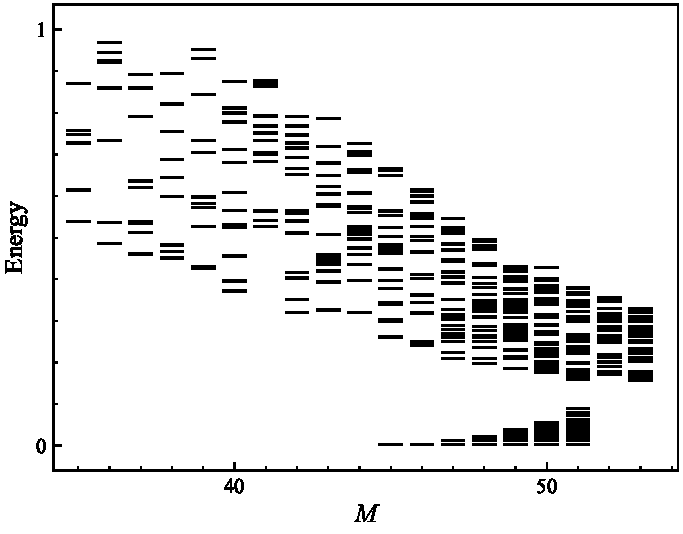
\includegraphics[width=0.72\textwidth]{fig_7.17.pdf}
\caption*{图 7.17\quad 六个电子的系统在前二十二个轨道中对于哈密顿量 $H_V$ 的能谱。$M=45,\ldots,51$ 处零能态的简并度分别求得为 $1,1,2,3,5,7,11$。}
\end{figure}

在下面，我们将从 Laughlin 波函数 $\Psi_m$ 出发计算准粒子/电子的等时关联。首先，我们如下计算 $|\xi\rangle=\prod_i(1-\frac{z_i}{\xi})^n\Psi_m(\{z_i\})$ 的模：
\begin{align*}
\langle\xi|\xi\rangle&=|\xi|^{-2Nn}\frac{Z_1}{Z}\tag{7.4.13}\\
Z&=\int\prod\mathrm{d}^2z_i\ \exp\Bigl(-\beta\sum_{ij}(-m^2)\ln|z_i-z_j|-\beta\sum_k\frac{m}{4}|z_k|^2\Bigr)\\
Z_1&=\int\prod\mathrm{d}^2z_i\ \exp\Bigl[\beta\sum_{ij}m^2\ln|z_i-z_j|-\beta\sum_k\Bigl(\frac{m}{4}|z_k|^2-nm\ln|\xi-z_k|\Bigr)\Bigr]
\end{align*}
其中 $\beta=2/m$。注意，$Z$ 是由 $N$ 个“电荷”为 $m$ 的粒子组成的等离子体的配分函数，而 $Z_1$ 是该等离子体与 $\xi$ 处一个“电荷”为 $n$ 的粒子发生相互作用的配分函数。我们可以写成
\begin{equation*}
Z=\mathrm{e}^{-\beta E},\qquad Z_1=\mathrm{e}^{-\beta E_1}
\end{equation*}
其中 $E$ 与 $E_1$ 是等离子体的总能量。能量的改变 $E_1-E$ 由加在 $\xi$ 处的“电荷” $n$ 粒子与 $z_i$ 处 $N$ 个“电荷” $m$ 粒子之间的相互作用给出。当 $|\xi|$ 大时，$N$ 个“电荷” $m$ 粒子形成一个圆形液滴，我们可以把它们当作 $z=0$ 处的一个点“电荷” $mN$ 来处理。我们得到 $E_1-E=-nmN\ln|\xi|$。对于较小的 $|\xi|$，“电荷” $n$ 会改变液滴的形状，此时
\begin{equation*}
E_1-E=-nmN\ln|\xi|-\frac{n^2}{2}\Bigl[-\ln\Bigl(|\xi|-\frac{R^2}{|\xi|}\Bigr)+\ln(|\xi|)\Bigr]
\tag{7.4.14}
\end{equation*}
其中 $R=\sqrt{mN}\,l_B$ 是液滴的半径。式 (7.4.14) 中的第一项是“电荷” $n$ 与\emph{未形变}液滴之间的相互作用。第二项是液滴形变引起的修正。由于等离子体的行为像金属，这一修正可以用“电荷” $n$ 与它在 $|z|=R^2/|\xi|$ 及 $z=0$ 处的镜像之间的相互作用来表示。

在上述讨论中，我们忽略了电荷的分立性，把等离子体当作连续介质来处理。我们预期，只要 $\xi$ 不太靠近液滴，即 $|\xi|-R\gg l_B$，这一近似就能给出正确的比值 $Z_1/Z$。

由式 (7.4.14)，我们求得 $|\psi^n(\xi)\rangle$ 的模为
\begin{equation*}
\langle\xi|\xi\rangle=\Bigl(\frac{\xi\xi^*}{\xi\xi^*-R^2}\Bigr)^{n^2/m}
\tag{7.4.15}
\end{equation*}
由于内积 $\langle\tilde{\xi}|\xi\rangle$ 是 $\xi$ 的全纯函数、$\tilde{\xi}$ 的反全纯函数，式 (7.4.15) 意味着
\begin{equation*}
\langle\tilde{\xi}|\xi\rangle=\Bigl(\frac{\xi\tilde{\xi}^*}{\xi\tilde{\xi}^*-R^2}\Bigr)^{n^2/m}
\end{equation*}
注意，当 $n=m$ 时，
\begin{equation*}
\xi^{Nm}\tilde{\xi}^{*Nm}\langle\tilde{\xi}|\xi\rangle=\xi^{Nm}\tilde{\xi}^{*Nm}\Bigl(\frac{\xi\tilde{\xi}^*}{\xi\tilde{\xi}^*-R^2}\Bigr)^m
\end{equation*}
正比于 $N_e=N+1$ 电子系统边缘上等时的电子传播子 $G_e$。取 $\xi=R\mathrm{e}^{\mathrm{i}\frac{x}{R}}$ 与 $\tilde{\xi}=R$，我们得到
\begin{equation*}
G_e(x)=L^{-m}a^{m-1}\mathrm{e}^{\mathrm{i}m\left(N_e-\frac{1}{2}\right)\frac{2\pi x}{L}}\sin^{-m}(\pi x/L)
\tag{7.4.16}
\end{equation*}
当 $x$ 远小于 $L\equiv2\pi R$（译注：原文印作“$21R$”，应为液滴周长 $2\pi R$）时，上式退化为式 (7.4.9)。这里 $a$ 是 $l_B$ 量级的一个长度标度。式 (7.4.16) 可以展开如下：
\begin{align*}
G_e(x)&=L^{-m}a^{m-1}\mathrm{e}^{\mathrm{i}m(N_e-1)\frac{2\pi x}{L}}\Bigl[\sum_{n=0}^{\infty}\mathrm{e}^{-\mathrm{i}\frac{2\pi x}{L}n}\Bigr]^m\notag\\
&=L^{-m}a^{m-1}\mathrm{e}^{\mathrm{i}m(N_e-1)\frac{2\pi x}{L}}\sum_{n=0}^{\infty}C_n^{m+n-1}\,\mathrm{e}^{-\mathrm{i}\frac{2\pi x}{L}n}\\
C_n^{m+n-1}&=\frac{(n+m-1)!}{(m-1)!\,n!}\tag{7.4.17}
\end{align*}

从这个展开，我们得到角动量 $M$ 态上的电子占据数 $n_M$ 如下：
\begin{equation*}
\begin{array}{ll}
n_M=0, & \delta M=m(N_e-1)-M<0\\[4pt]
n_M=\dfrac{a^{m-1}}{L^{m-1}}C_{\delta M}^{\delta M+m-1}, & \delta M\geqslant0
\end{array}
\tag{7.4.18}
\end{equation*}
我们看到，费米边缘的准确位置处在最后一个部分占据的单粒子轨道上，即处在角动量 $m(N_e-1)$ 处（或 $k_F=\sqrt{m(N_e-1)}/l_B$ 处）。注意，当 $m(N_e-1)-M\gg m$ 时，我们有 $n_M\propto(m(N_e-1)-M)^{m-1}$。用沿边缘的动量来表示，我们有 $n_k\propto(k_F-k)^{m-1}$。我们发现，与费米液体不同，占据数 $n_k$ 在费米动量处没有跳跃。

我们想指出，式 (7.4.16) 只在 $x$ 远大于磁长度 $l_B$ 时才正确。因此，式 (7.4.18) 只在 $m(N_e-1)-M\ll\sqrt{N_e}$ 时才有效。

如果边缘激发的色散是线性的，那么在低能下 $G_e$ 只能依赖于 $x-vt$。我们立刻看到，含时的电子格林函数为
\begin{equation*}
G_e(x,t)=L^{-m}a^{m-1}\mathrm{e}^{\mathrm{i}m\left(N-\frac{1}{2}\right)\frac{2\pi(x-vt)}{L}}\sin^{-m}[\pi(x-vt)/L]
\end{equation*}
当 $m=1$ 时，上式成为一维自由费米子的电子格林函数（对费米点附近的 $k$）。

\subsection{流体动力学方法——2/5 与 2/3 态}

\begin{keypoints}
\item 分级 FQH 液体的边缘态。
\item 电子算符与准粒子算符的结构。
\item 当且仅当边缘激发能够沿相反方向传播时，边缘相互作用才能修改电子/准粒子传播子的指数。
\item 当 $\nu_1=-\nu_2=1$ 时，本节的讨论描述一维 Tomonaga--Luttinger 液体。
\end{keypoints}

在这一节中，我们将用流体动力学方法研究第二级分级态的边缘结构。我们将以 2/5 态与 2/3 态为例。特别地，我们将研究分级态边缘上电子算符与准粒子算符的结构。我们还将看到，2/3 态包含两支沿相反方向传播的边缘模式，这是相当反直觉的。

首先，让我们考虑 $\nu=\frac{2}{5}$ 的 FQH 态。按照分级理论，$\nu=\frac{2}{5}$ 的 FQH 态是在 $\nu=\frac{1}{3}$ 的 FQH 态之上凝聚准粒子而生成的。因此，2/5 态包含两种不可压缩流体组分。为了明确起见，让我们考虑一个特殊的边缘势，使得 FQH 态由两个液滴组成（见图 7.14）：一个是电子凝聚体，填充因子为 $\nu_1=\frac{1}{3}$，半径为 $r_1$；另一个是准粒子凝聚体（位于 1/3 态之上），填充因子为 $\nu_2=\frac{1}{15}$（注意 $\frac{1}{3}+\frac{1}{15}=\frac{2}{5}$），半径为 $r_2<r_1$。

当 $r_1-r_2\gg l_B$ 时，两条边缘相互独立。推广 7.4.2 节的流体动力学方法，可以证明存在两支边缘激发，其低能动力学由下式描述：
\begin{equation*}
\begin{gathered}
[\rho_{Ik},\rho_{Jk'}]=\frac{\nu_I}{2\pi}k\delta_{IJ}\delta_{k+k'}\\
H=2\pi\sum_{I,k>0}\frac{v_I}{\nu_I}\rho_{I,-k}\rho_{I,k}
\end{gathered}
\tag{7.4.19}
\end{equation*}
其中 $I=1,2$ 标记两支，$v_I$ 是边缘激发的速度。在式 (7.4.19) 中，$\rho_I$ 是一维电子密度。为了使哈密顿量下有界，我们要求 $\nu_Iv_I>0$。我们发现，$\nu=\frac{2}{5}$ FQH 态的稳定性要求两个 $v_I$ 都为正。

推广 7.4.2 节的讨论，两条边缘上的电子算符为
\begin{equation*}
\Psi_I=\mathrm{e}^{\mathrm{i}\frac{1}{\nu_I}\phi_I(x)},\qquad I=1,2
\tag{7.4.20}
\end{equation*}
其中 $\partial_x\phi_I=\frac{1}{2\pi}\rho_I$。电子传播子具有形式
\begin{equation*}
\langle T(\Psi_I(x,t)\Psi_I^\dagger(0))\rangle=\frac{\mathrm{e}^{\mathrm{i}k_Ix}}{(x-v_I t)^{-1/|\nu_I|}},\qquad I=1,2
\end{equation*}
这里 $k_I=r_I/2l_B^2$。

按照分级图像，$\nu=\frac{2}{3}$ 的 FQH 态也是由两个凝聚体形成的：一个填充因子为 1 的电子凝聚体和一个填充因子为 $-\frac{1}{3}$ 的空穴凝聚体。因此，取 $(\nu_1,\nu_2)=(1,-\frac{1}{3})$，上述讨论同样可以应用于 $\nu=\frac{2}{3}$ 的 FQH 态。同样存在两支边缘激发，但只要哈密顿量是正定的，这两支现在就具有\emph{相反}的速度。

当我们把两条边缘靠拢到 $r_1-r_2\sim l_B$ 时，两支边缘激发之间的相互作用不再可以忽略。此时，哈密顿量具有形式
\begin{equation*}
H=2\pi\sum_{k>0}V_{IJ}\rho_{I,-k}\rho_{J,k}
\tag{7.4.21}
\end{equation*}

哈密顿量 (7.4.21) 可以对角化。当 $\nu_1\nu_2>0$ 时，我们可以选择
\begin{align*}
\tilde{\rho}_{1k}&=\cos(\theta)\frac{1}{\sqrt{|\nu_1|}}\rho_{1k}+\sin(\theta)\frac{1}{\sqrt{|\nu_2|}}\rho_{2k}\\
\tilde{\rho}_{2k}&=\cos(\theta)\frac{1}{\sqrt{|\nu_2|}}\rho_{2k}-\sin(\theta)\frac{1}{\sqrt{|\nu_1|}}\rho_{1k}\\
\tan(2\theta)&=2\frac{\sqrt{|\nu_1\nu_2|}V_{12}}{|\nu_1|V_{11}-|\nu_2|V_{22}}
\tag{7.4.22}
\end{align*}
可以检验，$\tilde{\rho}$ 满足
\begin{equation*}
\begin{gathered}
[\tilde{\rho}_{Ik},\tilde{\rho}_{Jk'}]=\frac{\operatorname{sgn}(\nu_I)}{2\pi}k\delta_{IJ}\delta_{k+k'}\\
H=2\pi\sum_{I,k>0}\operatorname{sgn}(\nu_I)\tilde{v}_I\tilde{\rho}_{I,-k}\tilde{\rho}_{I,k}
\end{gathered}
\tag{7.4.23}
\end{equation*}
其中边缘激发的新速度 $\tilde{v}_I$ 由下式给出：
\begin{align*}
\operatorname{sgn}(\nu_1)\tilde{v}_1&=\frac{\cos^2(\theta)}{\cos(2\theta)}|\nu_1|V_{11}-\frac{\sin^2(\theta)}{\cos(2\theta)}|\nu_2|V_{22}\\
\operatorname{sgn}(\nu_2)\tilde{v}_2&=\frac{\cos^2(\theta)}{\cos(2\theta)}|\nu_2|V_{22}-\frac{\sin^2(\theta)}{\cos(2\theta)}|\nu_1|V_{11}
\tag{7.4.24}
\end{align*}
我们看到仍然有两支边缘激发。然而在这种情况下，具有确定速度的边缘激发是内边缘上的激发与外边缘上的激发的混合。还可以证明，只要哈密顿量 (7.4.21) 下有界，两支的速度 $\tilde{v}_I$ 就总是正的。

通过反解式 (7.4.22) 把式 (7.4.20) 中的电子算符 $\Psi_I$ 用 $\tilde{\rho}_I$ 重写之后，我们可以利用式 (7.4.24) 计算它们的传播子如下：
\begin{equation*}
\langle T(\Psi_I(x,t)\Psi_I^\dagger(0))\rangle=\mathrm{e}^{\mathrm{i}k_Ix}\frac{1}{(x-\tilde{v}_1t)^{\alpha_I}}\frac{1}{(x-\tilde{v}_2t)^{\beta_I}}
\end{equation*}
其中
\begin{equation*}
(\alpha_1,\alpha_2)=\Bigl(\frac{\cos^2\theta}{|\nu_1|},\frac{\sin^2\theta}{|\nu_2|}\Bigr),\qquad
(\beta_1,\beta_2)=\Bigl(\frac{\sin^2\theta}{|\nu_1|},\frac{\cos^2\theta}{|\nu_2|}\Bigr)
\end{equation*}

然而，当两条边缘靠近到磁长度以内时，$\Psi_I$ 就不再是边缘上最普遍的电子算符了。普遍的电子算符可以包含两边缘之间的电荷转移。对 $\nu=2/5$ 的 FQH 态，内边缘与外边缘之间隔着 $\nu=\frac{1}{3}$ 的 Laughlin 态。因此，基本的电荷转移算符由下式给出：
\begin{equation*}
\eta(x)=\mathrm{e}^{\mathrm{i}(\phi_1-\frac{\nu_1}{\nu_2}\phi_2)}=(\Psi_1\Psi_2^\dagger)^{\nu_1}
\end{equation*}
它把一份 $\nu_1e=e/3$ 的电荷从外边缘转移到内边缘。普遍的电子算符于是具有形式
\begin{equation*}
\begin{gathered}
\Psi(x)=\sum_{n=-\infty}^{+\infty}c_n\psi_n(x)\\
\psi_n(x)=\Psi_1(x)\eta^n(x)
\end{gathered}
\tag{7.4.25}
\end{equation*}

为了理解这个结果，我们注意到，无论整数 $n$ 取何值，每个算符 $\psi_n$ 总是产生一个单位的局域电荷，并且是费米性算符。因此，每个 $\psi_n$ 都是边缘电子算符的一个候选者。对一个普遍的相互作用系统，边缘上的电子算符预期是不同 $\psi_n$ 的叠加，如式 (7.4.25) 所表示。注意 $\Psi_2=\psi_{-1/\nu_1}$。$\psi_n$ 的传播子可以用与上面概述类似的方法计算，结果为
\begin{equation*}
\langle T(\psi_n(x,t)\psi_m^\dagger(0))\rangle\propto\delta_{n,m}\,\mathrm{e}^{\mathrm{i}[k_1+n\nu_1(k_2-k_1)]x}\prod_I(x-\tilde{v}_It)^{-\gamma_{In}}
\end{equation*}
其中 $\gamma_{In}$ 为
\begin{align*}
\gamma_{1n}&=\Bigl[\Bigl(n+\frac{1}{|\nu_1|}\Bigr)\sqrt{|\nu_1|}\cos\theta-\frac{n\nu_1}{\nu_2}\sqrt{|\nu_2|}\sin\theta\Bigr]^2\\
\gamma_{2n}&=\Bigl[\Bigl(n+\frac{1}{|\nu_1|}\Bigr)\sqrt{|\nu_1|}\sin\theta+\frac{n\nu_1}{\nu_2}\sqrt{|\nu_2|}\cos\theta\Bigr]^2
\tag{7.4.26}
\end{align*}

从式 (7.4.25) 与上式（译注：原文作“式 (7.4.4)”，应指上面未编号的 $\psi_n$ 传播子公式）我们看到，电子传播子在分立动量 $k=k_1+n\nu_1(k_2-k_1)$ 处具有奇异性。它们类似于相互作用一维电子系统中电子传播子的 $k_F,3k_F,\ldots$ 奇异性。

对 $\nu=\frac{2}{3}$ 的 FQH 态，我们有 $\nu_1\nu_2<0$。在这种情况下，我们需要选择
\begin{align*}
\tilde{\rho}_{1k}&=\cosh(\theta)\frac{1}{\sqrt{|\nu_1|}}\rho_{1k}+\sinh(\theta)\frac{1}{\sqrt{|\nu_2|}}\rho_{2k}\\
\tilde{\rho}_{2k}&=\cosh(\theta)\frac{1}{\sqrt{|\nu_2|}}\rho_{2k}+\sinh(\theta)\frac{1}{\sqrt{|\nu_1|}}\rho_{1k}\\
\tanh(2\theta)&=2\frac{\sqrt{|\nu_1\nu_2|}V_{12}}{|\nu_1|V_{11}+|\nu_2|V_{22}}
\tag{7.4.27}
\end{align*}
来对角化哈密顿量。可以检验，$\tilde{\rho}_I$ 同样满足 K--M 代数 (7.4.23)，只是现在
\begin{align*}
\operatorname{sgn}(\nu_1)\tilde{v}_1&=\frac{\cosh^2(\theta)}{\cosh(2\theta)}|\nu_1|V_{11}-\frac{\sinh^2(\theta)}{\cosh(2\theta)}|\nu_2|V_{22}\\
\operatorname{sgn}(\nu_2)\tilde{v}_2&=\frac{\cosh^2(\theta)}{\cosh(2\theta)}|\nu_2|V_{22}-\frac{\sinh^2(\theta)}{\cosh(2\theta)}|\nu_1|V_{11}
\tag{7.4.28}
\end{align*}
同样，只要哈密顿量 $H$ 是正定的，边缘激发的速度 $\tilde{v}_I$ 就总是具有相反的符号。电子算符仍具有 (7.4.25) 的形式，其中 $\eta=(\Psi_1\Psi_2^\dagger)^{\nu_1}$。$\psi_n$ 的传播子仍由式 (7.4.4)（译注：同前，应指上面未编号的 $\psi_n$ 传播子公式）给出，其中
\begin{align*}
\gamma_{1n}&=\Bigl[\Bigl(n+\frac{1}{|\nu_1|}\Bigr)\sqrt{|\nu_1|}\cosh\theta+\frac{n\nu_1}{\nu_2}\sqrt{|\nu_2|}\sinh\theta\Bigr]^2\\
\gamma_{2n}&=\Bigl[\Bigl(n+\frac{1}{|\nu_1|}\Bigr)\sqrt{|\nu_1|}\sinh\theta+\frac{n\nu_1}{\nu_2}\sqrt{|\nu_2|}\cosh\theta\Bigr]^2
\tag{7.4.29}
\end{align*}

在等空间点处，电子算符 $\psi_n$ 的长时间关联由总指数 $g_e^{(n)}$ 控制如下：
\begin{equation*}
\langle\psi_n^\dagger(0,t)\psi_n(0,0)\rangle\sim t^{-g_e^{(n)}},\qquad g_e^{(n)}=\sum_I\gamma_{In}
\end{equation*}

等空间的电子关联决定了边缘隧穿实验中的 $I$--$V$ 曲线（见 3.7.4 节与 4.2.2 节）。指数的最小值 $g_e\equiv\operatorname{Min}(g_e^{(n)})$ 控制着电子在两边缘之间隧穿的标度性质。例如，隧穿电导在有限温度下的标度行为为
\begin{equation*}
\sigma\propto T^{2g_e-2}
\end{equation*}
对 $\nu=2/5$ 态，这里 $g_e=3$。对 $\nu=2/3$ 态，$g_e$ 依赖于两边缘之间的相互作用。

\subsection*{问题 7.4.6}

\textbf{一维相互作用费米子系统的玻色化}考虑一个自由的一维费米子模型
\begin{equation*}
H_0=\sum_k\epsilon_k:c_k^\dagger c_k:
\end{equation*}
正规排序定义为：当 $\epsilon_k>0$ 时 $:c_k^\dagger c_k:=c_k^\dagger c_k$；当 $\epsilon_k<0$ 时 $:c_k^\dagger c_k:=-c_kc_k^\dagger$。这里当 $k=\pm k_F$ 时 $\epsilon_k=0$。
\begin{enumerate}
\item 令 $\rho_{1,k}=\sum_{q\sim k_F}^{\prime}:c_q^\dagger c_{q+k}:$，其中求和 $\sum_{q\sim k_F}^{\prime}$ 限制在使 $c_{q+k}$ 与 $c_q$ 的动量都处于范围 $[-\Lambda+k_F,+\Lambda+k_F]$ 之内的那些项。令 $\rho_{2,k}=\sum_{q\sim-k_F}^{\prime}:c_q^\dagger c_{q+k}:$，其中求和 $\sum_{q\sim-k_F}^{\prime}$ 使 $c_{q+k}$ 与 $c_q$ 处于范围 $[-\Lambda-k_F,+\Lambda-k_F]$ 之内。这里 $k<\Lambda<k_F$。我们注意到，$\rho_{1,k}$ 在 $k_F$ 附近产生右行激发，而 $\rho_{2,k}$ 在 $-k_F$ 附近产生左行激发。证明 $\rho_{I,k}$ 满足 K--M 代数 (7.4.19)，其中 $\nu_1=1$，$\nu_2=-1$。证明 $H_0=2\pi v_F\sum_{k>0}(\rho_{1,k}\rho_{1,-k}-\rho_{2,-k}\rho_{2,k})$。于是一维自由费米子系统可以被玻色化。
\item 我们可以把电子算符写成 $c(x)=\psi_1(x)+\psi_2(x)$，其中 $\psi_1(x)=\sum_{-\Lambda+k_F}^{\Lambda+k_F}\mathrm{e}^{\mathrm{i}kx}c_k$ 是 $k_F$ 附近的电子算符，而 $\psi_2(x)=\sum_{-\Lambda-k_F}^{\Lambda-k_F}\mathrm{e}^{\mathrm{i}kx}c_k$ 是 $-k_F$ 附近的电子算符。试用 $\phi_I$ 表示 $c(x)$，这里 $(2\pi)^{-1}\partial_x\phi_I(x)=\rho_I(x)$。
\item 为了验证一维相互作用费米子系统也可以被玻色化，证明相互作用项 $H_V=\sum_{q,k_1,k_2}V_q\allowbreak(c_{k_1}^\dagger c_{k_1+q})\allowbreak(c_{k_2}^\dagger c_{k_2+q})$ 在限制到两个费米点附近时变为 $2\pi\sum\allowbreak V_{IJ}\rho_{I,-k}\rho_{J,k}+$ 常数。求 $V_{IJ}$。
\item 计算相互作用模型 $H_0+H_V$ 的电子格林函数 $\langle c^\dagger(x,t)c(0)\rangle$。
\end{enumerate}

\subsection{体有效理论与边缘态}

\begin{keypoints}
\item 边缘态的结构可以由以 $K$ 矩阵表征的体拓扑序直接确定。
\end{keypoints}

在这一节中，我们将从体 FQH 态的 Chern--Simons 有效理论直接导出边缘激发的宏观理论。在这种方法中，我们不依赖于 FQH 态的任何具体构造。体拓扑序与边缘态之间的关系变得十分清楚。我必须提醒读者，本节所给出的计算是非常形式的。结果的正确性不是由形式计算来保证的，而是由与其他独立计算（例如 7.4.3 节中的那个）的比较来保证的。

为了理解有效理论与边缘态之间的关系，让我们先考虑填充因子 $\nu=1/m$ 的最简单 FQH 态，并尝试由体有效理论重新导出 7.4.2 节的结果。这样的 FQH 态由具有作用量
\begin{equation*}
S=-\frac{m}{4\pi}\int a_\mu\partial_\nu a_\lambda\varepsilon^{\mu\nu\lambda}\mathrm{d}^3x
\tag{7.4.30}
\end{equation*}
的 U(1) Chern--Simons 理论描述。

假设我们的样品具有一个边界。为简单起见，我们假设边界是 $x$ 轴，样品覆盖下半平面。

对于带边界的 FQH 液体，有效作用量 (7.4.30) 存在一个问题：由于边界的存在，它在规范变换 $a_\mu\to a_\mu+\partial_\mu f$ 下不是不变的，即 $\Delta S=-\frac{m}{4\pi}\int_{y=0}\mathrm{d}x\mathrm{d}t\,f(\partial_ta_1-\partial_1a_0)$。为了解决这个问题，我们将把规范变换限制为在边界上为零：$f(x,y=0,t)=0$。由于这一限制，$a_\mu$ 在边界上的一些自由度变成了动力学自由度。

我们知道，有效理论 (7.4.30) 只是针对无边界的体 FQH 态导出的。这里，我们将把带有受限规范变换的式 (7.4.30) 取作为带边界的 FQH 态的有效理论的定义。这样的定义肯定是自洽的。下面我们将证明，这样的定义重现了 7.4.2 节所得到的结果。

研究规范理论动力学的一种方法是选择规范条件 $a_0=0$，并把 $a_0$ 的运动方程当作一个约束。对 Chern--Simons 理论，这样的约束成为 $f_{ij}=0$。在这个约束下，我们可以把 $a_i$ 写成 $a_i=\partial_i\phi$。把它代入式 (7.4.30)，就得到边缘上一个有效的一维理论，其作用量为（Elitzur et al., 1989）
\begin{equation*}
S_{\text{edge}}=-\frac{m}{4\pi}\int\partial_t\phi\,\partial_x\phi\,\mathrm{d}x\mathrm{d}t
\tag{7.4.31}
\end{equation*}

然而，这个方法有一个问题。容易看出，与作用量 (7.4.31) 相联系的哈密顿量为零，而且式 (7.4.31) 所描述的边界激发的速度为零。因此，这个作用量不能用来描述真实 FQH 样品中任何物理的边缘激发。FQH 态中的边缘激发总是具有有限的速度。

边缘激发出现有限速度是一种边界效应。由式 (7.3.18) 定义的体有效理论不包含边缘激发速度的信息。为了从有效理论确定边缘激发的动力学，我们必须找到一种把边缘速度的信息输入进来的办法。边缘速度必须被当作体有效理论中不包含的外部参量来处理。问题在于如何把这些参量放进理论之中。

现在让我们注意到，$a_0=0$ 这个条件并不是规范固定条件的唯一选择。更普遍的规范固定条件具有形式
\begin{equation*}
a_\tau=a_0+va_x=0
\tag{7.4.32}
\end{equation*}
这里 $a_x$ 是矢量势平行于样品边界的分量，而 $v$ 是一个具有速度量纲的参量。

方便的做法是选择满足
\begin{equation*}
\tilde{x}=x-vt,\qquad \tilde{t}=t,\qquad \tilde{y}=y.
\tag{7.4.33}
\end{equation*}
的新坐标。注意，在坐标变换下规范势 $a_\mu$ 按 $\partial/\partial x^\mu$ 变换。我们发现在新坐标下，规范场的各分量
% ——— 块边界说明（起点）———
% 书页 326（p341）末句为 "We find that in the new coordinates the components of
%     the gauge field"，跨页延续到书页 327（p342）顶部 "are given by" + 式 (7.4.34)。
% 上半句译文（"我们发现，在新坐标下规范场的各分量"）由 ch7_d 收尾；
% 本块正文以 %JOIN% 起头，从"由下式给出"+式 (7.4.34) 续起，与 ch7_d 末句缝合。
% ——— 块边界说明（终点）———
% 本块为章末块：书页 334（p349）止于问题 7.4.9，其后空白，第 7 章自然收束
% （书页 335 即第 8 章章首），故本块不设 %--D-TAIL-- 区。
% ——— 覆盖范围 ———
% §7.4.5 后部（自式 (7.4.34) 起，含式 (7.4.35)–(7.4.37)、问题 7.4.7、脚注 49）；
% §7.4.6 全节（式 (7.4.38)–(7.4.48)、问题 7.4.8、脚注 50）；
% §7.4.7 全节（图 7.18、表 7.3、式 (7.4.49)、问题 7.4.9）。
% ——————————————————————————————
由下式给出：
\begin{equation*}
\tilde{a}_{\tilde{t}}=a_{t}+va_{x},\qquad \tilde{a}_{\tilde{x}}=a_{x},\qquad \tilde{a}_{\tilde{y}}=a_{y}. \tag{7.4.34}
\end{equation*}
在新坐标下，规范固定条件就化为前面讨论过的那个条件。容易看出，在式 (7.4.33) 与式 (7.4.34) 给出的变换下，Chern--Simons 作用量的形式保持不变：
\begin{equation*}
S=-\frac{m}{4\pi}\int\mathrm{d}^{3}x\,a_{\mu}\partial_{\nu}a_{\lambda}\varepsilon^{\mu\nu\lambda}
=-\frac{m}{4\pi}\int\mathrm{d}^{3}x\,\tilde{a}_{\tilde{\mu}}\partial_{\tilde{\nu}}\tilde{a}_{\tilde{\lambda}}\varepsilon^{\tilde{\mu}\tilde{\nu}\tilde{\lambda}}
\end{equation*}
重复前面的推导，我们发现边缘作用量为
\begin{equation*}
S=-\frac{m}{4\pi}\int\mathrm{d}\tilde{t}\,\mathrm{d}\tilde{x}\,\partial_{\tilde{t}}\phi\,\partial_{\tilde{x}}\phi
\end{equation*}
用原来的物理坐标表示，上述作用量具有形式
\begin{equation*}
S=-\frac{m}{4\pi}\int\mathrm{d}t\,\mathrm{d}x\,(\partial_{t}+v\partial_{x})\phi\,\partial_{x}\phi \tag{7.4.35}
\end{equation*}
这是一个手征玻色子理论（chiral boson theory）(Gross et al., 1985; Floreanini and Jackiw, 1988)。由运动方程 $\partial_{t}\phi+v\partial_{x}\phi=0$ 可以看出，式 (7.4.35) 所描述的边缘激发具有非零的速度 $v$，并且只朝一个方向运动。

为了得到式 (7.4.35) 的量子理论，我们需要把手征玻色子理论量子化。量子化可以在动量空间中进行：
\begin{equation*}
S=\frac{m}{2\pi}\int\mathrm{d}t\sum_{k>0}\left(\mathrm{i}k\dot{\phi}_{k}\phi_{-k}-vk^{2}\phi_{k}\phi_{-k}\right).
\end{equation*}
可以证明，如果我们把 $k>0$ 的 $\phi_{k}$ 视为``坐标''，那么 $\phi_{-k}$ 将正比于与之对应的动量 $\pi_{k}=\partial S/\partial\dot{\phi}_{k}$。辨认出``坐标''与``动量''之后，我们便可以得到哈密顿量以及对易关系 $[\phi_{k},\pi_{k^{\prime}}]=\mathrm{i}\delta_{kk^{\prime}}$，它们完全定义了这个量子系统。如果引入 $\rho=\frac{1}{2\pi}\partial_{x}\phi$，我们发现该量子系统由下式描述：
\begin{equation*}
[\rho_{k},\rho_{k^{\prime}}]=\frac{k\delta_{k+k^{\prime}}}{2\pi m},\qquad
H=2\pi mv\sum_{k>0}\rho_{k}^{\dagger}\rho_{k} \tag{7.4.36}
\end{equation*}

边缘激发的速度 $v$ 通过规范固定条件进入我们的理论。注意，在受限规范变换下，具有不同 $v$ 的规范固定条件 (7.4.32) 彼此不能互相变换，它们在物理上并不等价。这与我们的假设一致：规范固定条件中的 $v$ 是一个物理参量，它实际上决定了边缘激发的速度。

哈密顿量 (7.4.36) 只有当 $vm<0$ 时才有下界。理论的自洽性要求 $v$ 与 $m$ 符号相反。因此，边缘激发速度的符号（即手性（chirality））由 Chern--Simons 项前面系数的符号决定。

由于矩阵 $K$ 可以对角化，上述结果可以容易地推广到式 (7.3.18) 所描述的一般 FQH 态。所得到的有效边缘理论具有形式
\begin{equation*}
S_{\mathrm{edge}}=\frac{1}{4\pi}\int\mathrm{d}t\,\mathrm{d}x\,\bigl[K_{IJ}\partial_{t}\phi_{I}\partial_{x}\phi_{J}-V_{IJ}\partial_{x}\phi_{I}\partial_{x}\phi_{J}\bigr] \tag{7.4.37}
\end{equation*}
哈密顿量为
\begin{equation*}
H_{\mathrm{edge}}=\frac{1}{4\pi}\int\mathrm{d}t\,\mathrm{d}x\,V_{IJ}\partial_{x}\phi_{I}\partial_{x}\phi_{J}
\end{equation*}
因此，$V$ 必须是正定矩阵。利用这个结果，可以证明 $K$ 的正本征值对应于一个左移分支，而负本征值对应于一个右移分支。

$\nu=2/5$ FQH 态的有效理论由 $K=\begin{pmatrix}3 & 2\\ 2 & 3\end{pmatrix}$ 给出。由于 $K$ 具有两个正本征值，$\nu=2/5$ FQH 态的边缘激发有两个朝同一方向运动的分支。$\nu=1-\frac{1}{n}$ FQH 态则由 $K=\begin{pmatrix}1 & 0\\ 0 & -n\end{pmatrix}$ 的有效理论描述。此时 $K$ 的两个本征值符号相反，因此边缘激发的两个分支朝相反的方向运动。

\subsection*{问题 7.4.7}
证明：量子化之后，系统 (7.4.35) 由式 (7.4.36) 描述。

\subsection{带电激发与电子传播子}

\begin{keypoints}
\item 一般 FQH 边缘上的一般电子/准粒子算符。
\end{keypoints}

我们已经研究了几种简单 FQH 液体中边缘激发的动力学，发现低能边缘激发由一个自由声子理论描述。本节我们将集中讨论一般的电荷激发。特别地，我们将对最一般的（阿贝尔）FQH 态计算电子与准粒子的传播子。关键点同样是把电子或准粒子算符用声子算符 $\rho_{I}$ 写出来。一旦做到这一点，传播子便可以容易地算出，因为在低能与长波极限下声子是自由的。

我们知道，对于式 (7.3.18) 所描述的 FQH 态，其边缘态由作用量 (7.4.37) 描述。边缘激发的希尔伯特空间构成 K--M 代数的一个表示
\begin{align*}
[\rho_{Ik},\rho_{Jk^{\prime}}]&=(K^{-1})_{IJ}\frac{1}{2\pi}k\,\delta_{k+k^{\prime}}\\
k,k^{\prime}&=\text{整数}\times\frac{2\pi}{L} \tag{7.4.38}
\end{align*}
其中 $\rho_{I}=\frac{1}{2\pi}\partial_{x}\phi_{I}$ 是 FQH 态中第 $I$ 个凝聚体的边缘密度，$I,J=1,\ldots,\kappa$，而 $\kappa$ 是 $K$ 的维数。边缘上的电子密度为
\begin{equation*}
\rho_{e}=-eq_{I}\rho_{I}
\end{equation*}
边缘激发的动力学由哈密顿量
\begin{equation*}
H=2\pi\sum_{IJ}V_{IJ}\rho_{I,-k}\rho_{J,k} \tag{7.4.39}
\end{equation*}
描述，其中 $V_{IJ}$ 是正定矩阵。

我们先尝试写出边缘上的准粒子算符 $\Psi_{\pmb{l}}$，它产生一个由 $l_{I}$ 标记的准粒子。我们知道，把准粒子插到边缘上会使第 $I$ 个凝聚体的边缘密度发生一个改变 $\delta\rho_{I}$（见式 (7.3.22)）。$\delta\rho_{I}$ 满足
\begin{equation*}
\int\mathrm{d}x\,\delta\rho_{I}=(\pmb{l}^{\top}K^{-1})_{I}.
\end{equation*}
由于 $\Psi_{\pmb{l}}$ 是一个只引起密度局域改变的局域算符，我们有
\begin{equation*}
[\rho_{I}(x),\Psi_{\pmb{l}}(x^{\prime})]=l_{J}(K^{-1})_{JI}\delta(x-x^{\prime})\Psi_{\pmb{l}}(x^{\prime}) \tag{7.4.40}
\end{equation*}
利用 Kac--Moody 代数 (7.4.38)，可以证明满足式 (7.4.40) 的准粒子算符为
\begin{equation*}
\Psi_{\pmb{l}}\propto\mathrm{e}^{\mathrm{i}\phi_{I}l_{I}} \tag{7.4.41}
\end{equation*}
准粒子 $\Psi_{\pmb{l}}$ 的电荷由对易子 $[\rho_{e},\Psi_{\pmb{l}}]$ 确定，结果为
\begin{equation*}
Q_{\pmb{l}}=-e\,\pmb{q}^{\top}K^{-1}\pmb{l} \tag{7.4.42}
\end{equation*}
由式 (7.3.24) 与式 (7.4.41)，我们看到电子算符可以写成
\begin{equation*}
\Psi_{e,L}\propto\mathrm{e}^{\mathrm{i}\sum_{I}l_{I}\phi_{I}},\qquad
l_{I}=K_{I,J}L_{J},\qquad q_{I}L_{I}=1 \tag{7.4.43}
\end{equation*}
由式 (7.4.42) 可见，上述算符携带单位电荷。$\Psi_{e,L}$ 的对易可如下计算：
\begin{align*}
\Psi_{e,L}(x)\Psi_{e,L}(x^{\prime})&=(-)^{\lambda}\Psi_{e,L}(x^{\prime})\Psi_{e,L}(x)\\
\lambda&=l_{I}(K^{-1})_{IJ}l_{J}=L_{I}K_{IJ}L_{J} \tag{7.4.44}
\end{align*}
在分级基（hierarchical basis）中，$K_{II}|_{I=1}$ 为奇数，$K_{II}|_{I>1}$ 为偶数，$\pmb{q}^{\top}=(1,0,\ldots,0)$，且 $L_{1}=1$。利用这些条件，我们可以证明 $(-)^{\lambda}=-1$。式 (7.4.43) 定义的电子算符的确是费米子算符。

由于不同 $L_{I}$ 选择下的所有算符 $\Psi_{e,L}$ 都携带单位电荷并且是费米型的，每一个 $\Psi_{e,L}$ 都可能是电子算符的候选。一般地，真正的电子算符是诸 $\Psi_{e,L}$ 的下述叠加：
\begin{equation*}
\Psi_{e}=\sum_{L}C_{L}\Psi_{e,L}
\end{equation*}
这里，当我们说边缘上存在许多不同的电子算符时，我们的真正意思是：真实的物理电子算符是这些算符的一个叠加。

利用 K--M 代数 (7.4.38) 与哈密顿量 (7.4.39)，我们可以计算一个一般准粒子算符
\begin{equation*}
\Psi_{\pmb{l}}\propto\mathrm{e}^{\mathrm{i}l_{I}\phi_{I}}
\end{equation*}
（对于 $\pmb{l}$ 的合适选择，其中包括电子算符）的传播子。首先，我们注意到变换
\begin{equation*}
\rho_{I}\rightarrow U_{IJ}\tilde{\rho}_{J}
\end{equation*}
把 $(V,K)$ 变为 $(\tilde{V},\tilde{K})=(U^{\top}VU,\,U^{\top}KU)$。选取合适的 $U$，$K$ 与 $V$ 可以被同时对角化；\footnote{由于 $V$ 是正定的对称矩阵，我们可以找到一个 $U_{1}$，它把 $V$ 变为 $V_{1}=U_{1}^{\top}VU_{1}=1$，把 $K$ 变为 $K_{1}=U_{1}^{\top}KU_{1}$。注意 $K_{1}$ 是一个对称矩阵，其本征值与 $K$ 的本征值同号（尽管它们的绝对值可以不同）。然后我们做一个正交变换把 $K_{1}$ 对角化，即 $(K_{1})_{IJ}\rightarrow(K_{2})_{IJ}=\sigma_{I}|v_{I}|^{-1}\delta_{IJ}$。在这个正交变换下，$V_{1}\rightarrow V_{2}=1$ 不变且保持对角。最后，我们用一个对角矩阵把 $K_{2}$ 缩放为 $(K_{3})_{IJ}=\sigma_{I}\delta_{IJ}$。这把 $V_{2}$ 变为 $V_{3}=|v_{I}|\delta_{IJ}$。新的 $(V_{3},K_{3})$ 便导致式 (7.4.45)。}用 $\tilde{\rho}_{I}$ 表示，式 (7.4.38) 与式 (7.4.39) 变为
\begin{align*}
[\tilde{\rho}_{Ik},\tilde{\rho}_{Jk^{\prime}}]&=\sigma_{I}\delta_{IJ}\frac{1}{2\pi}k\,\delta_{k+k^{\prime}}\\
H&=2\pi\sum_{I,k>0}|v_{I}|\,\tilde{\rho}_{I,-k}\tilde{\rho}_{I,k} \tag{7.4.45}
\end{align*}
其中 $\sigma_{I}=\pm1$ 是 $K$ 本征值的符号。由 $\tilde{\rho}_{I}$ 产生的边缘激发的速度为 $v_{I}=\sigma_{I}|v_{I}|$。

用 $\tilde{\rho}_{I}$ 表示，算符 $\Psi_{\pmb{l}}$ 具有形式
\begin{equation*}
\Psi_{\pmb{l}}\propto\mathrm{e}^{\mathrm{i}\sum_{I}\tilde{l}_{I}\tilde{\phi}_{I}},\qquad
\tilde{l}_{J}=l_{I}U_{IJ} \tag{7.4.46}
\end{equation*}
由式 (7.4.45) 与式 (7.4.46)，我们看到 $\Psi_{\pmb{l}}$ 的传播子具有以下一般形式：
\begin{equation*}
\langle\Psi_{\pmb{l}}^{\dagger}(x,t)\Psi_{\pmb{l}}(0)\rangle\propto
\mathrm{e}^{\mathrm{i}l_{I}k_{I}x}\prod_{I}(x-v_{I}t+\mathrm{i}\sigma_{I}\delta)^{-\gamma_{I}},\qquad
\gamma_{I}=\tilde{l}_{I}^{2} \tag{7.4.47}
\end{equation*}
其中 $v_{I}=\sigma_{I}|v_{I}|$ 是边缘激发的速度。右移成分的总指数减去左移成分的总指数，满足求和规则\footnote{我们用到了
$\lambda_{\pmb{l}}=\sum_{I,J,I^{\prime}}l_{I^{\prime}}U_{I^{\prime}I}\sigma_{I}(U^{\top})_{I,J}l_{J}$，以及
$(K^{-1})_{IJ}=U_{II^{\prime}}\sigma_{I^{\prime}}\delta_{I^{\prime},J^{\prime}}(U^{\top})_{J^{\prime},J}$。}
\begin{equation*}
\sum_{I}\sigma_{I}\gamma_{I}\equiv\lambda_{\pmb{l}}=\pmb{l}^{\top}K^{-1}\pmb{l} \tag{7.4.48}
\end{equation*}
我们看到，差值 $\lambda_{\pmb{l}}$ 不依赖边缘相互作用 $V$，是一个拓扑量子数。由式 (7.4.44) 与式 (7.4.48)，我们看到这个差值与 $\Psi_{\pmb{l}}$ 的统计性质直接相关。如果 $\Psi_{\pmb{l}}$ 代表电子算符（或其他费米型算符），那么 $\lambda_{\pmb{l}}$ 将是一个奇整数。从式 (7.4.47) 我们还看到，算符 $\Psi_{\pmb{l}}$ 产生的激发带有接近 $\sum_{I}l_{I}k_{I}$ 的动量。

\subsection*{问题 7.4.8}
证明式 (7.4.41) 中的 $\Psi_{\pmb{l}}$ 满足式 (7.4.40)。

\subsection{手征 Luttinger 液体的唯象后果}

\begin{keypoints}
\item 三类边缘态。
\item 长程相互作用与杂质散射的效应。
\end{keypoints}

在前四节中，我们已经证明 FQH 液体边缘上的电子构成手征 Luttinger 液体。作为手征 Luttinger 液体的特征性质之一，电子与准粒子的传播子获得如下的反常指数（anomalous exponents）：
\begin{equation*}
\langle\Psi_{e}^{\dagger}(t,x=0)\Psi_{e}(0)\rangle\sim t^{-g_{e}},\qquad
\langle\Psi_{q}^{\dagger}(t,x=0)\Psi_{q}(0)\rangle\sim t^{-g_{q}}
\end{equation*}
这些反常指数可以通过 FQH 边缘之间的隧穿实验直接测量。

\begin{figure}[H]
\centering
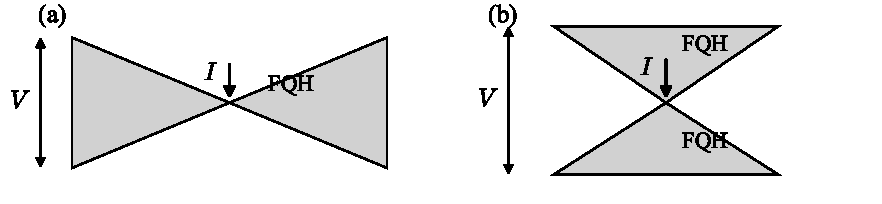
\includegraphics[width=0.72\textwidth]{fig_7.18.pdf}
\caption*{图 7.18\quad (a) 同一 FQH 态的两条边缘之间的准粒子隧穿。(b) 不同 FQH 态的边缘之间的电子隧穿。}
\end{figure}

以下两种情形需要分开考虑：(i) 两条 FQH 液体边缘被一个绝缘体隔开；(ii) 两条边缘被一个 FQH 液体隔开。情形 (i) 中，只有电子能够在两条边缘之间隧穿（见图 7.18(b)）；情形 (ii) 中，隔开两条边缘的 FQH 液体所支持的准粒子能够隧穿（见图 7.18(a)）。情形 (i) 的隧穿算符为 $A\propto\Psi_{e1}\Psi_{e2}^{\dagger}$，其中 $\Psi_{e1}$ 与 $\Psi_{e2}$ 是两条边缘上的电子算符；情形 (ii) 的隧穿算符具有形式 $A\propto\Psi_{q1}\Psi_{q2}^{\dagger}$，其中 $\Psi_{q1}$ 与 $\Psi_{q2}$ 是两条边缘上的准粒子算符。隧穿的物理性质可以由隧穿算符的关联函数算出，而后者又可以表示为两条边缘上电子或准粒子传播子的乘积。

令 $g=g_{e}$ 对应情形 (i)，$g=g_{q}$ 对应情形 (ii)。那么在零温下，电子与准粒子算符的反常指数导致 $\langle A(t)A(0)\rangle\propto|t|^{-2g}$，从而给出一条非线性的隧穿 $I$--$V$ 曲线（见 3.7.4 节）
\begin{equation*}
I\propto V^{2g-1}
\end{equation*}
隧穿电流的噪声谱在频率 $f=QV/h$ 处还包含一个奇异性，即
\begin{equation*}
S(f)\sim\bigl|f-\frac{QV}{h}\bigr|^{2g-1} \tag{7.4.49}
\end{equation*}
其中 $V$ 是两条边缘之间的电压差，$Q$ 是隧穿电子或隧穿准粒子的电荷。在有限温度 $T$ 下，零偏压电导也具有如下幂律依赖关系：
\begin{equation*}
\sigma\propto T^{2g-2}
\end{equation*}
我们看到，反常指数可以很容易地通过隧穿实验测量。噪声谱还进一步揭示了隧穿粒子的电荷。

指数 $g_{e}$ 与 $g_{q}$ 已在 7.4.6 节中算出。为了以简单的方式总结这些结果，最好把 FQH 边缘分成以下两类：(A) 所有边缘激发朝同一方向运动；(B) 边缘激发朝两个方向传播。

对于 A 类边缘，指数 $g_{e}$ 与 $g_{q}$ 与电子及准粒子的统计性质直接相关。在这种情形下，$g_{e}$ 与 $g_{q}$ 是普适的，不依赖电子相互作用和边缘势的细节。表 7.3 列出了一些支持 A 类边缘态的 FQH 态，以及相应的指数 $g_{e,q}$ 的数值和相应粒子的电荷（注意表中只列出了 $g_{e}$ 与 $g_{q}$ 的最小值）。

\begin{center}
\small 表 7.3\quad 具有 A 类边缘态的某些 FQH 态的 $(g_{e},g_{q},Q_{q})$\\[6pt]
\begin{tabular}{cccccc}
\toprule
FQH 态 & $\nu=1/m$ & $\nu=2/5$ & $\nu=p/(pq+1)$ & $(331)_{\nu=1/2}$ & $(332)_{\nu=2/5}$ \\
\midrule
$g_{e}$ & $m$ & $3$ & $q+1$ & $3$ & $3$ \\
$g_{q}$ & $1/m$ & $2/5$ & $p/(pq+1)$ & $3/8$ & $2/5$ \\
电荷 $Q_{q}/e$ & $1/m$ & $2/5$ & $p/(pq+1)$ & $1/4$ & $2/5$ \\
\bottomrule
\end{tabular}
\end{center}

让我们讨论一下，对于填充因子为 $\nu=\frac{p}{pq+1}$（$q=$ 偶数）的分级态，上述结果是如何得到的。这些态包括 $\nu=2/5,3/7,2/9,\ldots$ 等 FQH 态。填充因子为 $\nu=\frac{p}{pq+1}$ 的分级态，在 $\pmb{q}^{\top}=(1,1,\ldots,1)$ 的基下由 $p\times p$ 矩阵 $K=1+qC$ 描述。这里 $C$ 是伪单位矩阵（pseudo-identity matrix），即 $C_{IJ}=1$，$I,J=1,\ldots,p$，而 $K^{-1}=1-\frac{q}{pq+1}C$。由于所有边缘激发都朝同一方向运动，我们有
\begin{equation*}
\langle\Psi_{\pmb{l}}^{\dagger}(x=0,t)\Psi_{\pmb{l}}(0)\rangle\propto t^{-\lambda_{\pmb{l}}}
\end{equation*}
其中 $\lambda_{\pmb{l}}$ 由式 (7.4.48) 给出。基本准粒子由 $\pmb{l}^{\top}=(1,0,\ldots,0)$ 给出，携带电荷 $\frac{1}{pq+1}$，其传播子中的指数为 $\lambda_{\pmb{l}}=1-\frac{q}{pq+1}$。指数最小的准粒子由 $\pmb{l}^{\top}=(1,\ldots,1)$ 给出，携带电荷 $\frac{p}{pq+1}$，指数为 $\lambda_{\pmb{l}}=\frac{p}{pq+1}$，它小于 $1-\frac{q}{pq+1}$（注意我们有 $q\geqslant2$ 与 $p\geqslant1$）。在低能下，正是这样的准粒子（携带电荷 $\frac{p}{pq+1}$）主导\emph{同一} FQH 流体两条边缘之间的隧穿（见 7.4.7 节）。

电子算符由 $\Psi_{e,L}=\Psi_{\pmb{l}}$（译注：原文排印为 $\psi_{\pmb{l}}$，应为 $\Psi_{\pmb{l}}$ 之误）给出，其中 $\pmb{l}$ 满足 $\sum_{I}l_{I}=pq+1$。传播子中的指数为 $\lambda_{\pmb{l}}=\sum l_{I}^{2}-q(pq+1)$。传播子中指数最小的电子算符由 $\pmb{l}^{\top}=(q,\ldots,q,q+1)$ 给出，最小指数的值为 $\lambda_{\pmb{l}}=q+1$。在低能下，正是这样的电子算符主导两个\emph{不同} FQH 流体边缘之间的隧穿。

对于 B 类边缘，$g_{e}$ 与 $g_{q}$ 不是普适的。它们的数值依赖于电子相互作用和边缘势。

\subsection*{问题 7.4.9}
利用有限电压 $V$ 下隧穿算符的关联 $\langle A(t)A(0)\rangle$，推导式 (7.4.49)。

 % 本文件由 scripts/assemble.py 自动装配，勿手改（改 parts/ 后重跑）
% 第8章 拓扑序与量子序——超越朗道理论

% 第8章 TOPOLOGICAL AND QUANTUM ORDER—BEYOND LANDAU'S THEORIES

\chapter{拓扑序与量子序——超越朗道理论}

在第 3、4、5 章中，我们详细讨论了几个相互作用的玻色子/费米子系统。这些简单的模型例示了朗道的对称性破缺理论（加上 RG 理论）和朗道的费米液体理论（加上微扰论）。这两套朗道理论解释了许多凝聚态系统的行为，构成了传统多体理论的基础。这三章的讨论仅触及了朗道理论及其丰富应用的表面。想进一步学习朗道理论（以及 RG 理论和微扰论）的读者，会发现 Abrikosov et al. (1975)、Ma (1976)、Mahan (1990)、Negele and Orland (1998) 以及 Chaikin and Lubensky (2000) 的书颇有帮助。

朗道的理论非常成功，以至于在很长一段时间里，人们找不到任何不能用朗道理论描述的凝聚态系统。五十年来，朗道理论统治着多体物理，并实质上定义了多体物理的范式。这么多年之后，一种普遍的信念业已形成：我们已经弄清了所有重要的概念，理解了物质一切形态的基本性质。多体理论已经走到尽头，成为一门多少算是完备的理论。剩下要做的，只是把朗道理论（加上重整化群图像）应用于各种不同的系统。

从这个视角来看，我们能够理解 Tsui et al. (1982) 所发现的分数量子霍尔（FQH）效应的重要性。FQH 效应开辟了凝聚态物理的新篇章。正如我们在上一章看到的，FQH 液体不能用费米液体理论描述。不同的 FQH 态具有相同的对称性，因而不能用朗道的对称性破缺理论描述。因此，FQH 态完全超出了两套朗道理论。FQH 液体的存在表明，在朗道理论的范式之外还存在一个新世界。近来的研究表明，这个新范式比朗道理论的范式丰富得多。本书第 7 至 10 章将致力于讨论朗道理论之外的新范式。

为了窥见凝聚态物理新范式之一斑，除 FQH 态之外，我们还将研究量子转子系统、硬芯玻色子系统和量子自旋系统。这些系统都是强关联的多体系统。通常，这些系统中的强关联会导致长程序和对称性破缺。然而，我们已经以玻色超流体和费米子 SDW 态为例讨论过长程序和对称性破缺。因此，为了研究朗道理论之外的世界，我们把注意力集中于那些不能用长程序和对称性破缺描述的量子液体态（例如 FQH 态）。

这些量子液体态代表着物质的新状态，其中包含一种全新的序——拓扑序/量子序。我将证明，这种新序可能对我们理解量子相与量子相变以及量子相中的无能隙激发产生深远的影响。特别地，拓扑序/量子序或许能为自然界中的光和电子（以及其他规范玻色子和费米子）提供一个起源。

在本章中，我们将对拓扑序/量子序作一般性的讨论，以描绘一幅更大的图景。我们将以 FQH 态和费米液体态为例，讨论拓扑序/量子序中的一些基本问题。拓扑序/量子序中的问题与议题和传统多体物理中的大不相同。在深入任何细致的计算之前，理解这些问题究竟是什么是非常重要的。

\section{物质的状态与序的概念}

\begin{keypoints}
\item 物质可以有许多不同的状态（或不同的相）。序的概念是为了表征物质不同状态中不同的内部结构而引入的。
\item 我们曾以为，不同的序由其不同的对称性来表征。
\end{keypoints}

在足够高的温度下，一切物质都以气体的形式存在。气体是最简单的态之一。气体中一个原子的运动几乎不依赖于其他分子的位置和运动。因此，气体是弱关联系统，不含任何内部结构。然而，随着温度的降低，原子的运动变得越来越相互关联。最终，原子形成非常规则的图案，晶体序随之发展起来。在晶体中，单个原子几乎无法自行移动。晶体中的激发总是对应于许多原子的集体运动（这些集体运动称为声子）。晶体是强关联态的一个例子。

随着 1900 年前后低温技术的发展，物理学家发现了许多新的物质态（例如超导体和超流体）。这些不同的态具有不同的内部结构，称为不同种类的序。序的精确定义涉及相变。如果我们能够（通过平滑地改变哈密顿量）把一个多体系统的两个态平滑地相互变换而不遇到相变（即不遇到自由能的奇点），那么这两个态就具有相同的序。如果不存在不经相变就把一个态变为另一个态的途径，那么这两个态就具有不同的序。我们注意到，我们的序的定义是一个等价类的定义。能够不经相变而相互连通的两个态被定义为等价。以这种方式定义的等价类称为普适类。具有不同序的两个态也可以说是属于不同普适类的两个态。按照我们的定义，水和冰具有不同的序，而水和水蒸气具有相同的序（见图 8.1）。

\begin{figure}[H]
\centering
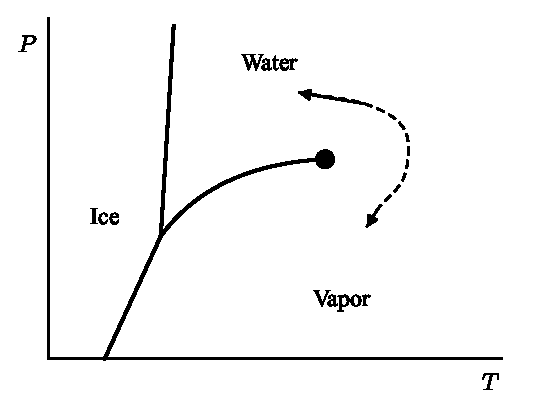
\includegraphics[width=0.72\textwidth]{fig_8.1.pdf}
\caption*{图 8.1\quad 水的相图。}
\end{figure}

在发现了如此多种不同的序之后，需要一个普遍理论以更深入地理解物质的态。特别地，我们想要理解，究竟是什么使两种序真正不同，以至于我们无法在不遇到相变的情况下把一种序变成另一种序。发展关于序以及相关的相与相变的普遍理论的关键一步，是认识到序与对称性相联系（更确切地说，与对称性的破缺相联系）。我们发现，当两个态具有不同的对称性时，我们无法在不遇到自由能奇点的情况下（即不经相变地）把一个态变为另一个态。基于序与对称性之间的这一关系，朗道发展了关于序以及不同序之间的相变的普遍理论（Ginzburg and Landau, 1950; Landau and Lifschitz, 1958）。朗道的理论非常成功。利用朗道理论和相关的对称性群论，我们可以对三维空间中可能存在的全部 230 种不同的晶体进行分类。通过确定对称性在连续相变处如何改变，我们可以得到相变的临界性质。对称性破缺还提供了许多无能隙激发的起源，例如声子、自旋波等，它们决定了许多系统的低能性质（Nambu, 1960; Goldstone, 1961）。这些激发的许多性质（包括其无能隙性）都直接由对称性决定。通过引入与对称性相联系的序参量，Ginzburg 和朗道发展了 Ginzburg--Landau 理论，它成为关于相与相变的标准理论。由于朗道的对称性破缺理论对我们理解物质具有如此广泛而根本的影响，它成了凝聚态理论的基石。朗道理论所描绘的图景令人如此满意，以至于人们开始有这样的感觉：至少在原则上，我们理解物质所能具有的一切种类的序。

\section{分数量子霍尔态中的拓扑序}

\begin{keypoints}
\item FQH 态开辟了凝聚态物理的新篇章，因为它是实验学家发现的第二个无法用对称性破缺和（局域）序参量来表征的态。
\item FQH 态包含一种新型的序——拓扑序。
\end{keypoints}

然而，自然界从不停止给我们带来惊喜。随着半导体技术的进步，物理学家学会了如何把电子限制在两种不同半导体之间的界面上，从而制成了二维电子气（2DEG）。1982 年，Tsui et al. (1982) 把二维电子气置于强磁场中，发现了一种新的物质态——FQH 液体（Laughlin, 1983）。由于温度低且电子之间的相互作用强，FQH 态是一个强关联态。然而，这样一个强关联态并不像人们原先预期的那样是晶体。事实证明，电子由于其质量非常之小而产生的强烈量子涨落阻止了晶体的形成。因此，FQH 态是一种量子液体。（晶体可以通过两种方式熔化：一是像我们升温时那样通过热涨落，得到普通的液体；二是像我们减小粒子质量时那样通过量子涨落，得到量子液体。）

正如我们在上一章看到的，量子霍尔液体具有许多令人惊叹的性质。量子霍尔液体比固体（晶体）更为“刚硬”，其含义是量子霍尔液体不可压缩。因此，量子霍尔液体具有固定且明确界定的密度。当我们用由下式定义的填充因子来度量电子密度时，
\begin{equation*}
\nu = \frac{\text{电子的密度}}{\text{磁通量子的密度}},
\end{equation*}
我们发现，所有已发现的量子霍尔态的密度都使填充因子恰好等于某些有理数，例如 $\nu = 1,\allowbreak 1/3,\allowbreak 2/3,\allowbreak 2/5,\allowbreak \ldots$。知道了 FQH 液体只存在于某些神奇的填充因子处，人们不禁猜测，FQH 液体应当具有某种内部的序或“图案”。不同的神奇填充因子应当来自这些不同的内部“图案”。然而，内部“图案”的假说看来有一个困难——FQH 态是液体，而液体怎么能有任何内部“图案”呢？

\begin{figure}[H]
\centering
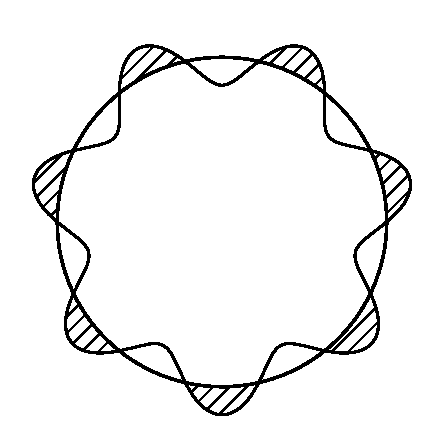
\includegraphics[width=0.72\textwidth]{fig_8.2.pdf}
\caption*{图 8.2\quad 圆周上的粒子波具有量子化的波长。}
\end{figure}

为了对 FQH 态中的内部序获得一些直观理解，让我们尝试设想 FQH 态中电子的量子运动。我们知道，根据量子物理，粒子也表现出波的行为。我们先考虑一个在圆周上以动量 $p$ 运动的粒子。这样一个粒子对应于波长为 $\lambda = h/p$ 的波，其中 $h$ 是普朗克常数。只有能够纳入圆周的波才是允许的（即圆周必须包含整数个波长）（见图 8.2）。于是，由于量子物理，粒子在圆周上的运动受到很强的限制（即量子化），只有某些分立的动量值才是允许的。这个量子化条件可以用更具图像感的方式来看待。我们可以说，粒子沿着圆周以步伐跳舞，步长由波长给出。量子化条件要求粒子总是用整数步走完圆周一圈。

现在让我们考虑磁场中的一个电子。在磁场的作用下，电子总是沿圆周运动（称为回旋运动）。在量子物理中，由于粒子的波动性质，只有某些分立的回旋运动是允许的。量子化条件要求：允许的回旋运动的圆形轨道包含整数个波长。我们可以说，电子总是用整数步走完圆周一圈。如果电子绕圆周走了 $n$ 步，我们就说电子处在第 $n$ 个朗道能级。第一朗道能级中的电子能量最低，低温下电子将停留在第一朗道能级。

当我们有许多电子构成二维电子气时，电子不仅在第一朗道能级中作各自的回旋运动，而且还会彼此绕行并交换位置。这些附加的运动同样服从量子化条件。例如，一个电子必须用整数步绕另一个电子一周。由于电子是费米子，交换两个电子会给波函数引入一个负号。而交换两个电子等价于让一个电子绕另一个电子走半程。因此，一个电子必须用半整数步绕另一个电子走半程。（半整数步给电子波函数引入一个负号。）换言之，一个电子必须用奇数步绕另一个电子一周。FQH 态中的电子不仅以满足量子化条件的方式运动，而且由于电子之间强烈的库仑排斥和费米统计，它们还尽可能地彼此远离。这意味着，只要可能，一个电子就试图用更多的步数绕另一个电子一周。

现在我们看到，尽管不存在晶体序，FQH 态中电子的量子运动却是高度有组织的。FQH 态中的所有电子集体起舞，遵循严格的跳舞规则。

\begin{enumerate}
\item 所有电子都在第一朗道能级中作各自的回旋运动，即它们用一步绕圆周一圈。
\item 一个电子总是用奇数步绕另一个电子一周。
\item 电子试图彼此远离，即它们试图用尽可能多的步数绕另一个电子一周。
\end{enumerate}

如果每个电子都遵循这些严格的跳舞规则，那么只允许唯一的一种整体跳舞图案。这样的跳舞图案描述了 FQH 态中的内部量子运动。正是这个整体跳舞图案对应于 FQH 态中的内部序。不同的 FQH 态由其不同的跳舞图案相互区分。

对上文概述的电子量子运动，更精确的数学描述由著名的 Laughlin 波函数给出（Laughlin, 1983）
\begin{equation*}
\Psi_m = \Bigl[\prod (z_i - z_j)^m\Bigr]\, \mathrm{e}^{-\frac{1}{4l_B^2}\sum |z_i|^2}
\end{equation*}
其中 $m$ 是奇整数，$z_j = x_j + i y_j$ 是第 $j$ 个电子的坐标。这样的波函数描述填充因子为 $\nu = 1/m$ 的 FQH 态。我们看到，当 $z_i \rightarrow z_j$ 时波函数变为零，因此电子不喜欢彼此靠得太近。此外，当我们把一个电子绕另一个电子移动一周时，波函数的相位改变 $2\pi m$。因此，在 Laughlin 态中，一个电子总是用 $m$ 步绕另一个电子一周。

我们想强调，FQH 液体的内部序（即跳舞图案）与其他关联系统（如晶体、超流体等）中的内部序非常不同。后一类系统中的内部序可以用与破缺对称性相联系的序参量来描述，因而有序态可以用 Ginzburg--Landau 有效理论来描述。FQH 液体中的内部序是一种新型的序，无法用与破缺对称性相联系的长程序来描述。\footnote{尽管有人建议用“非对角长程序”（Girvin and MacDonald, 1987）来表征 Laughlin 态的内部结构，但具有长程序的那个算符本身并不是局域算符。对于局域算符而言，既不存在长程序，也不存在对称性破缺的 Laughlin 态。}1989 年，人们引入了“拓扑序”的概念来描述 FQH 液体中这种新型的序（Wen, 1990, 1995）。

我们想指出，拓扑序是零温下任何具有有限能隙的态的普遍性质。非平庸的拓扑序不仅出现在 FQH 液体中，也出现在零温下的自旋液体中。事实上，拓扑序的概念正是在手征自旋液体（Kalmeyer and Laughlin, 1987; Khveshchenko and Wiegmann, 1989; Wen et al., 1989）的研究中首次引入的（Wen, 1990）。除手征自旋液体外，在任意子超流体（Chen et al., 1989; Fetter et al., 1989; Wen and Zee, 1991）以及自旋系统的短程共振价键态（Kivelson et al., 1987; Rokhsar and Kivelson, 1988; Read and Chakraborty, 1989; Read and Sachdev, 1991; Wen, 1991a）中也发现了非平庸的拓扑序。FQH 液体甚至还不是实验上观察到的第一个具有非平庸拓扑序的态。这份荣誉属于 1911 年发现的超导态（Onnes, 1911; Bardeen et al., 1957）。与通常的观点相反，具有动力学电磁相互作用的超导态不能用破缺的对称性来表征。它既没有长程序，也没有局域序参量。超导态包含非平庸的拓扑序，它与超流态有着根本的不同（Coleman and Weinberg, 1973; Halperin et al., 1974; Fradkin and Shenker, 1979）。

把 FQH 液体与晶体作比较是富有启发性的。FQH 液体与晶体的相似之处在于，二者都包含丰富的内部图案（即内部序）。主要区别在于，晶体中的图案是静态的，与原子的位置相关；而 QH 液体中的图案是“动态的”，与电子彼此“跳舞”的方式相关。然而，关于晶体序可以提出的许多同样的问题，对拓扑序也应当提出并加以解决。我们知道，晶体序可以用对称性来表征和分类。于是，一个重要的问题是：我们如何表征和分类拓扑序？我们还知道，晶体序可以用 X 射线衍射来测量。第二个重要的问题是：我们如何在实验上测量拓扑序？

下面我们将更详细地讨论 FQH 态中的拓扑序。事实证明，FQH 态是相当典型的拓扑有序态。许多其他拓扑有序态与 FQH 态有许多相似的性质。

\subsection{拓扑序的表征}

\begin{keypoints}
\item 物理学中的任何新概念都必须借助实验可测的量来引入（或定义）。定义一个物理量或一个概念，就是设计一个实验。
\item 拓扑序的概念（部分地）由基态简并度定义，该简并度对能够破坏所有对称性的\emph{任何}微扰都是稳健的。
\end{keypoints}

在上文中，拓扑序的概念（跳舞图案）是通过基态波函数引入的。这并不十分正确，因为基态波函数不是普适的。要确立一个新概念（例如拓扑序），就需要找到拓扑序的物理表征或测量方法。换言之，需要找到普适的量子数，它们对任何微扰（诸如相互作用、有效质量等的改变）都稳健，但对不同类别的 FQH 液体可以取不同的值。这类量子数的存在蕴含着拓扑序的存在。

显示 FQH 液体中存在拓扑序的一种途径，是研究它们的基态简并度（在热力学极限下）。FQH 液体有一个非常特殊的性质：它们的基态简并度依赖于空间的拓扑（Haldane, 1983; Haldane and Rezayi, 1985）。例如，$\nu = 1/q$ 的 Laughlin 态在亏格为 $g$ 的黎曼面上具有 $q^g$ 个简并基态。FQH 液体中的基态简并并\emph{不}是哈密顿量的对称性的结果。基态简并度对任意微扰都稳健（甚至是破坏哈密顿量中所有对称性的杂质）（Wen and Niu, 1990）。基态简并度的稳健性表明，导致基态简并的内部结构是普适而稳健的，从而证明了普适内部结构——拓扑序——的存在。

为了理解 FQH 基态的拓扑简并，我们考虑环面上的 $\nu = 1/m$ Laughlin 态。我们将用两种方法来计算基态简并度。第一种方法考虑如下隧穿过程：我们先产生一个准粒子--准空穴对；然后让准粒子绕环面一整周；最后湮灭准粒子--准空穴对，回到基态。这样一个隧穿过程产生一个把基态映射到基态的算符。若准粒子沿 $x$ 方向绕环面一周，该算符记为 $U_x$；若沿 $y$ 方向绕环面一周，则记为 $U_y$（见图 8.3(a,b)）。于是，沿 $x$、$y$、$-x$、$-y$ 四个方向的四次隧穿生成 $U_y^{-1}U_x^{-1}U_yU_x$（见图 8.3(c)）。我们注意到，上述四次隧穿的路径可以变形为两个相互链接的回路（见图 8.3(d)）。这两个相互链接的回路对应于让一个准粒子绕另一个准粒子一周，它产生一个相位 $\mathrm{e}^{2\mathrm{i}\theta}$，其中 $\theta$ 是准粒子的统计角。对 $1/m$ Laughlin 态，我们有 $\theta = \pi/m$。因此我们得到
\begin{equation*}
U_y^{-1}U_x^{-1}U_yU_x = \mathrm{e}^{\mathrm{i}2\pi/m}
\end{equation*}

\begin{figure}[H]
\centering
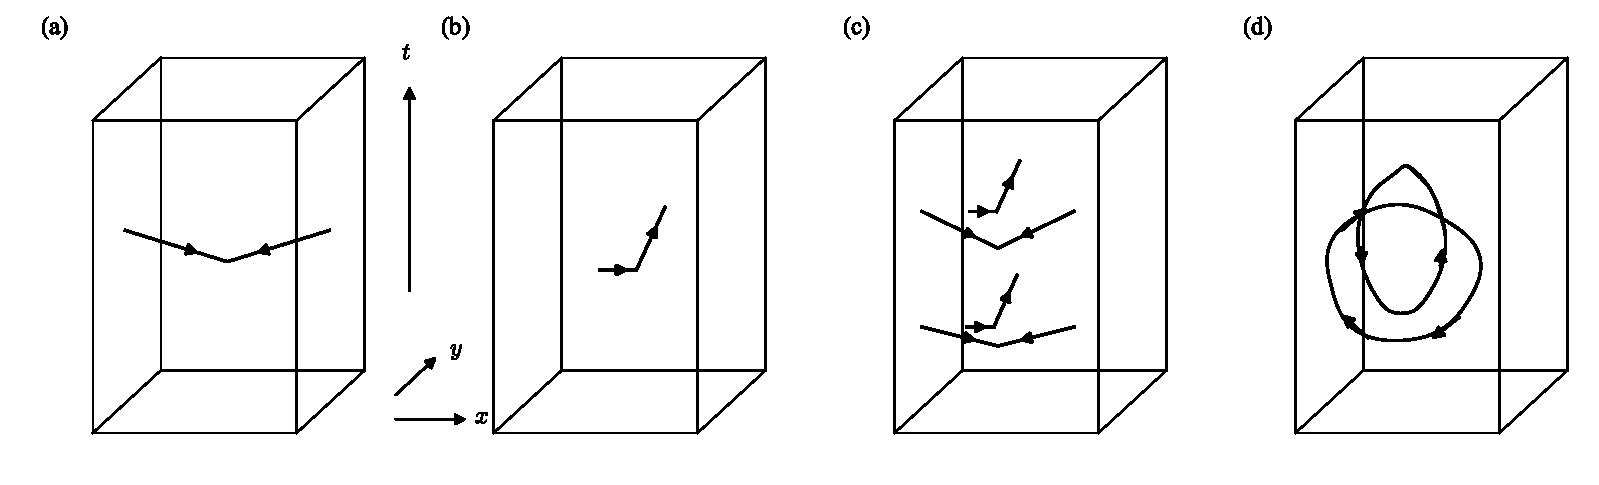
\includegraphics[width=0.72\textwidth]{fig_8.3.pdf}
\caption*{图 8.3\quad (a) 沿 $x$ 方向的隧穿产生 $U_x$。(b) 沿 $y$ 方向的隧穿产生 $U_y$。(c) 沿 $x$、$y$、$-x$ 和 $-y$ 方向的四次隧穿产生 $U_y^{-1}U_x^{-1}U_yU_x$。(d) 上述四次隧穿可以变形为两个相互链接的回路。}
\end{figure}

由于 $U_{x,y}$ 作用在基态之内，基态构成上述代数的表示。该代数只有一个 $m$ 维不可约表示。因此，$1/m$ Laughlin 态具有 $m \times$ 整数个简并基态。这一途径使我们能够直接看到准粒子统计与基态简并度之间的联系。

计算基态简并度的第二种方法是利用有效理论 (7.3.11)。简并的基态来自以下的集体涨落：
\begin{equation*}
a_i(t, x, y) = \theta_i(t)/L, \qquad i = x, y \tag{8.2.1}
\end{equation*}
其中 $L$ 是环面在 $x$ 和 $y$ 方向上的尺寸。所有其他涨落都产生非零的“磁”场 $b = f_{xy}$，并具有有限的能隙，这一点从经典运动方程可以看出。把式 (8.2.1) 代入式 (7.3.11)，可以得到描述式 (8.2.1) 中集体激发动力学的下列拉格朗日量：
\begin{equation*}
L = - \frac{m}{4\pi} (\dot{\theta}_x \theta_y - \dot{\theta}_y \theta_x) + \frac{1}{2g_1} \dot{\theta}_i^2. \tag{8.2.2}
\end{equation*}

由于 $a_\mu$ 的荷以整数量子化，作用在准粒子场 $\psi_q \to U\psi_q$ 上的规范变换 $U(x,y)$ 必须是环面上的周期函数。因此，规范变换必具有形式 $U(x,y) = \exp\bigl(2\pi\mathrm{i}\bigl(\frac{nx}{L} + \frac{my}{L}\bigr)\bigr)$，其中 $n$ 和 $m$ 是整数。由于 $\psi_q$ 的 $a_\mu$ 荷为 1，这样的规范变换按下式把规范场 $a_i$ 变为 $a_i' = a_i - \mathrm{i}U^{-1}\partial_i U$：
\begin{equation*}
(a_x', a_y') = \Bigl(a_x + \frac{2\pi n}{L},\ a_y + \frac{2\pi m}{L}\Bigr) \tag{8.2.3}
\end{equation*}

式 (8.2.3) 蕴含，$(\theta_x, \theta_y)$ 与 $(\theta_x + 2\pi n, \theta_y + 2\pi m)$ 规范等价，应当认同为同一位形。规范不等价的位形由环面 $0 < \theta_i < 2\pi$ 上的一个点给出。于是，拉格朗日量 (8.2.2) 描述一个单位电荷的粒子在以 $(\theta_x, \theta_y)$ 为参数的环面上运动。

式 (8.2.2) 的第一项表明，环面上存在均匀的“磁”场 $B = m/2\pi$。穿过环面的总通量等于 $2\pi \times m$。式 (8.2.2) 的哈密顿量为
\begin{equation*}
H = \frac{g_1}{2} \Bigl[- (\partial_{\theta_x} - \mathrm{i} A_{\theta_x})^2 - (\partial_{\theta_y} - \mathrm{i} A_{\theta_y})^2 \Bigr]. \tag{8.2.4}
\end{equation*}

式 (8.2.4) 的能量本征态形成朗道能级。朗道能级之间的能隙为 $g_1$ 的量级，与系统的尺寸无关。第一朗道能级中的态的数目等于穿过环面的磁通量子的数目，在我们的情形是 $m$。因此，$1/m$ Laughlin 态的基态简并度为 $m$。

为了理解基态简并度的稳健性，让我们在电子哈密顿量上加一个任意微扰。这样的微扰将引起有效拉格朗日量的改变 $\delta\mathcal{L}(a_\mu)$。这里的关键是，$\delta\mathcal{L}(a_\mu)$ 只通过场强依赖 $a_\mu$。换言之，$\delta\mathcal{L}$ 是 $e$ 和 $b$ 的函数。由于式 (8.2.1) 中的集体涨落在局域上是纯规范，$e$ 和 $b$ 从而 $\delta\mathcal{L}$ 都不依赖 $\theta_i$。$\delta\mathcal{L}(a_\mu)$ 不能在 $\theta_i$ 的有效理论中生成任何势项 $V(\theta_i)$；它只能生成仅依赖 $\dot{\theta}_i$ 的项。这样的修正重整化 $g_1$ 的数值，不能解除简并。

更一般的 FQH 态由式 (7.3.18) 描述。当 $K$ 为对角矩阵时，上述结果意味着基态简并度为 $\det(K)$。事实证明，对于一般的 $K$，基态简并度同样由 $\det(K)$ 给出。在亏格为 $g$ 的黎曼面上，基态简并度变为 $(\det(K))^g$。

我们看到，在紧致空间上，FQH 液体的低能物理非常独特。低能激发只有有限多个（即那些简并基态），然而低能动力学却是非平庸的，因为基态简并度依赖于空间的拓扑。这类只依赖于空间拓扑的特殊低能动力学由所谓的拓扑场论描述；拓扑场论在高能物理界曾被深入研究（Witten, 1989; Elitzur et al., 1989; Fr\"{o}hlich and King, 1989）。拓扑理论是 FQH 液体的有效理论，正如 Ginzburg--Landau 理论是超流体（或其他对称性破缺相）的有效理论。

基态简并度对空间拓扑的依赖表明，尽管所有局域物理算符都不具有长程关联，FQH 液体中仍存在某种长程序（即上面提到的整体跳舞图案）。在某种意义上，我们可以说 FQH 液体包含着隐藏的长程序。

% 实际覆盖范围说明：书页 345（p360）顶部为 8.2.2 节标题（非 8.3 节），故本块实际含
% 8.2.2、8.2.3、8.3、8.3.1、8.3.2、问题 8.3.1 与 8.4 节。
% 块界说明：书页 345 顶部为新节标题，无前块溢出内容，无 JOIN；
% 书页 353（p368）以一段正文自然收束全章，其后整页空白（p369 为第 9 章章首），无 TAIL。

\subsection{拓扑序的分类}

\begin{keypoints}
\item 理解拓扑序背后的数学框架是十分重要的。（正如理解群论——对称性破缺序背后的数学框架——十分重要一样。）
\item 对数学框架的理解将使我们能够对所有可能的拓扑序进行分类。
\end{keypoints}

如何标记和分类 FQH 液体中丰富的拓扑序，是一个长期悬而未决的问题。我们之所以能够对所有的晶体序进行分类，是因为我们知道晶体序由一个对称群描述。然而，我们对 FQH 液体中拓扑序的了解非常贫乏，拓扑序背后的数学结构尚不清楚。

尽管如此，对于一类 FQH 液体——阿贝尔 FQH 液体（Blok and Wen, 1990a,b; Read, 1990; Fröhlich and Kerler, 1991; Fröhlich and Studer, 1993）——我们还是找到了一种简单而统一的处理方法。Laughlin 态是最简单的阿贝尔 FQH 态，只含一种不可压缩流体组分。更一般的阿贝尔 FQH 态，其填充因子如 $\nu=2/5,3/7,\ldots$，含有数种不可压缩流体组分，并具有更复杂的拓扑序。阿贝尔 FQH 态中的拓扑序（或称跳舞图案（dancing patterns））同样可以用舞步来描述。跳舞图案可以用一个整数对称矩阵 $K$ 和一个整数电荷矢量 $\pmb{q}$ 来刻画。$\pmb{q}$ 的一个分量 $q_{i}$，是不可压缩流体第 $i$ 种组分中的粒子所携带的电荷（以 $e$ 为单位）。$K$ 的一个矩阵元 $K_{ij}$，是第 $i$ 种组分的粒子绕第 $j$ 种组分的粒子走一圈所迈的步数。在 FQH 态的 $(K,\pmb{q})$ 表征中，$\nu=1/m$ 的 Laughlin 态由 $K=m$、$\pmb{q}=1$ 描述，而 $\nu=2/5$ 的阿贝尔态由 $K=\begin{pmatrix}3&2\\2&3\end{pmatrix}$、$\pmb{q}=\begin{pmatrix}1\\1\end{pmatrix}$ 描述。

与拓扑序相关联的所有物理性质都可以用 $K$ 和 $\pmb{q}$ 定出。例如，填充因子就简单地由 $\nu=\pmb{q}^{\top}K^{-1}\pmb{q}$ 给出，而基态在亏格为 $g$ 的黎曼面上的简并度是 $\det(K)^{g}$。这一类 FQH 液体中所有的准粒子激发都具有阿贝尔统计，“阿贝尔 FQH 液体”由此得名。

上述对 FQH 液体的分类并不完全。并非每个 FQH 态都能用 $K$ 矩阵描述。1991 年，一类新的 FQH 态——非阿贝尔 FQH 态——被提出（Moore and Read, 1991; Wen, 1991b）。非阿贝尔 FQH 态含有具有非阿贝尔统计的准粒子。实验观察到的填充因子为 $\nu=5/2$ 的 FQH 态（Willett et al., 1987）很可能就是这样一个态（Haldane and Rezayi, 1988a,b; Greiter et al., 1991; Read and Green, 2000）。许多研究（Moore and Read, 1991; Blok and Wen, 1992; Iso et al., 1992; Cappelli et al., 1993; Wen et al., 1994）揭示了 FQH 态中的拓扑序与共形场论之间的联系。然而，对于非阿贝尔态中所有可能的拓扑序的完全分类，我们仍然相去甚远。

\subsection{边缘激发——测量拓扑序的一种实用方法}

\begin{keypoints}
\item FQH 态的边缘激发扮演着类似于 X 射线之于晶体的角色。我们可以利用边缘激发在实验上探测 FQH 态中的拓扑序。换言之，与基态简并度相比，边缘激发为拓扑序提供了更完全的定义。
\end{keypoints}

基态的拓扑简并只能部分地刻画拓扑序。不同的拓扑序有时会导致相同的基态简并度。这里的问题是，我们能否对拓扑序有更完全的刻画/测量。认识到拓扑序既不能用局域序参量、也不能用局域算符的长程关联来刻画之后，似乎很难再找到任何刻画拓扑序的方法。令人惊奇的是，FQH 态以一种出人意料的方式找到了出路。FQH 态体内的拓扑序可以用边缘激发来刻画/测量（Wen, 1992）。这种二维拓扑序编码在一维边缘态中的现象，与超弦理论和量子引力中的全息原理有若干相似之处（'t Hooft, 1993; Susskind, 1995）。\footnote{译注：原文为 holomorphic principle（全纯原理），疑为 holographic principle（全息原理）之误，此处按本意译出。}

作为不可压缩液体，FQH 液体的所有体内激发都有有限的能隙。然而，有限大小的 FQH 液体总是含有一维的无能隙边缘激发，这是 FQH 流体的另一个独特性质。边缘激发的结构极为丰富，这反映了体内丰富的拓扑序。不同的体内拓扑序导致不同的边缘激发结构。因此，我们可以通过研究边缘激发的结构来研究和测量体内的拓扑序。

正如我们在上一章所看到的，由于非平庸的体内拓扑序，（阿贝尔）FQH 液体边缘上的电子形成一类新的关联态——手征 Luttinger 液体（Wen, 1992）。手征 Luttinger 液体中的电子传播子获得一个反常指数：$\langle c^{\dagger}(t,x)c(0)\rangle\propto(x-vt)^{-g}$，$g\neq1$。（对费米液体，我们有 $g=1$。）在许多情形下，指数 $g$ 是一个拓扑量子数，不依赖于边缘的细节性质。因此，$g$ 是一个可用于刻画 FQH 液体中拓扑序的新量子数。许多实验组已经通过两条边缘之间隧穿电导的温度依赖关系成功地测量了指数 $g$（Milliken et al., 1995; Chang et al., 1996），理论预言其形式为 $\sigma\propto T^{2g-2}$（Wen, 1992）。这一实验证实了新型手征 Luttinger 液体的存在，并为在实验上研究 FQH 液体丰富的体内与边缘结构打开了大门。

\begin{figure}[H]
\centering
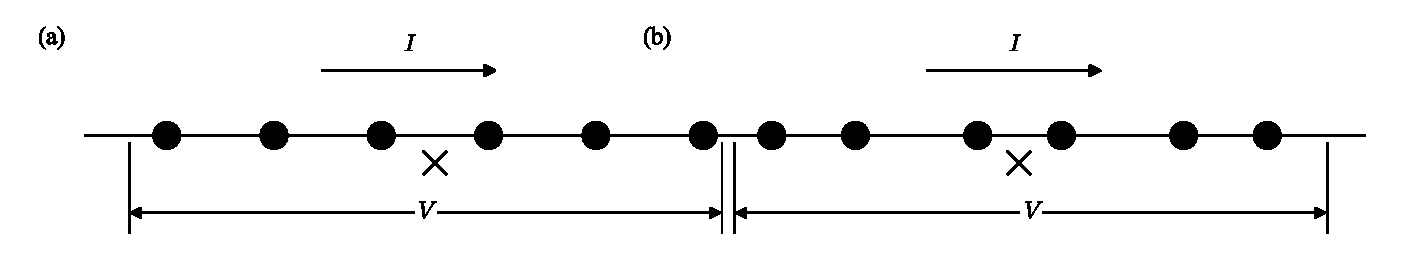
\includegraphics[width=0.72\textwidth]{fig_8.4.pdf}
\caption*{图 8.4\quad 一维晶体经过杂质时，将在电压降中产生窄带噪声。}
\end{figure}
\begin{figure}[H]
\centering
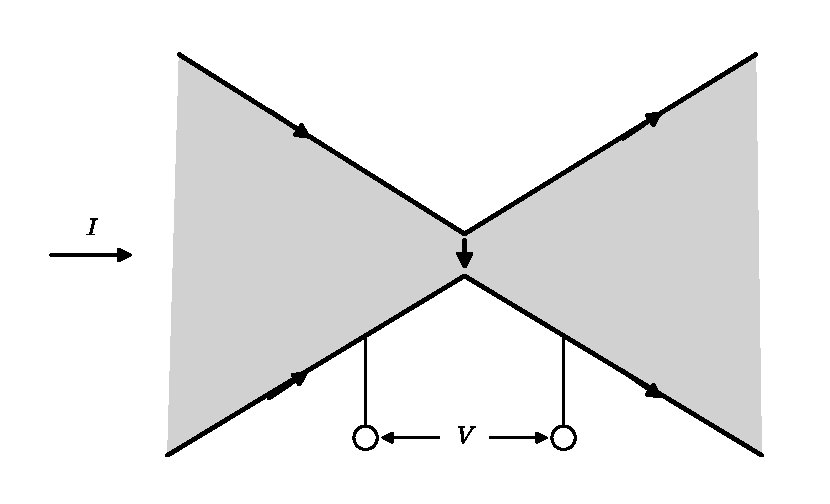
\includegraphics[width=0.72\textwidth]{fig_8.5.pdf}
\caption*{图 8.5\quad FQH 流体流经收缩区（constriction）时，由于准粒子的背散射而产生窄带噪声。}
\end{figure}

非阿贝尔 FQH 液体的边缘态构成更为奇异的一维关联系统，这类系统迄今尚未被命名。人们发现，这些边缘态与 $1+1$ 维共形场论密切相关（Wen et al., 1994）。

我们知道，晶体序可以用 X 射线衍射实验来测量。下面我们想提出：FQH 液体中的拓扑序可以（原则上）通过边缘输运实验中的噪声谱来测量。让我们先考虑一个被驱动着通过杂质的一维晶体（见图 8.4(a)）。由于晶体序的存在，如果每个元胞只含一个带电粒子，杂质两侧的电压在频率 $f=I/e$ 处具有窄带噪声。更精确地说，噪声谱具有一条奇异性，即 $S(f)\sim A\delta(f-\frac{I}{e})$。如果每个元胞含有两个带电粒子（见图 8.4(b)），那么我们将在 $f=I/2e$ 处看到一条额外的窄带噪声，于是 $S(f)\sim B\delta(f-\frac{I}{2e})+A\delta(f-\frac{I}{e})$。在这个例子中我们看到，噪声谱使我们能够测量一维情形中的晶体序。类似的实验也可用于测量 FQH 液体中的拓扑序。让我们考虑一个带有窄收缩区的 FQH 样品（见图 8.5）。收缩区通过两条边缘之间的准粒子隧穿诱导背散射。背散射使收缩区两侧的电压出现噪声。在弱背散射极限下，噪声谱在某些频率处含有奇异性，这使我们能够测量 FQH 液体中的拓扑序。\footnote{此处给出的讨论仅适用于其边缘激发全部沿同一方向传播的 FQH 态。对于阿贝尔态，这要求 $K$ 的所有本征值都具有相同的符号。}更具体地，噪声谱中的奇异性具有如下形式（见式 (7.4.49)）
\begin{equation*}
S(f)\sim\sum_{a}C_{a}|f-f_{a}|^{\gamma_{a}}\tag{8.2.5}
\end{equation*}
奇异性的频率与指数 $(f_{a},\gamma_{a})$ 由拓扑序决定。对于由矩阵 $K$ 和电荷矢量 $\pmb{q}$ 表征的阿贝尔态，$(f_{a},\gamma_{a})$ 的允许取值为
\begin{equation*}
f_{a}=\frac{I}{e\nu}\pmb{q}^{\top}K^{-1}\pmb{l},\qquad\gamma_{a}=2\pmb{l}^{\top}K^{-1}\pmb{l}-1\tag{8.2.6}
\end{equation*}
其中 $\pmb{l}^{\top}=(l_{1},l_{2},\ldots)$ 是任意整数矢量，$\nu=\pmb{q}^{\top}K^{-1}\pmb{q}$ 是填充因子。噪声谱中的奇异性由两条边缘之间的准粒子隧穿引起。奇异性的频率 $f_{a}$ 由隧穿准粒子的电荷 $Q_{q}$ 决定，即 $f_{a}=\frac{I}{e}\frac{Q_{q}}{e\nu}$。指数 $\gamma_{a}$ 由隧穿准粒子的统计 $\theta_{q}$ 决定，即 $\gamma=2\frac{|\theta_{q}|}{\pi}-1$。于是，噪声谱测量的是允许存在的准粒子的电荷与统计，而这又决定了 FQH 态中的拓扑序。

\section{量子序}

\begin{keypoints}
\item 量子态一般包含一种新的序——量子序（quantum order）。量子序无法完全用破缺的对称性及相应的序参量来刻画。
\item 量子序描述多体基态中量子纠缠的图案。
\item 量子序的涨落可以产生无能隙规范玻色子和无能隙费米子。量子序保护这些激发的无能隙性，正如对称性保护对称性破缺态中的无能隙 Nambu--Goldstone 玻色子一样。
\item 拓扑序是量子序的一种特殊情形，其中所有激发都具有有限的能隙。
\end{keypoints}

按定义，拓扑序只描述有能隙量子态的内部序。这里我们做一次信念上的飞跃。我们将假设能隙并不重要，无能隙量子态同样可以包含无法用对称性和长程关联描述的序。我们将把量子基态中的非对称性破缺序称为量子序。

如果你相信这条思路，那么剩下要做的事情只有两件：证明量子序确实存在，并找到刻画量子序的数学描述（或符号）。我们将在 8.3.2 节和第 10 章中证明量子序确实存在。由于量子序不能用破缺的对称性和序参量来刻画，我们需要发展一个新的理论来描述量子序。目前，我们还没有一个能够描述所有可能量子序的完整理论。然而，在第 9 章中我们设法找到了一个数学对象——投影对称群（projective symmetry group, PSG）——它能够描述一大类量子序。

有人可能会问，为什么我们需要引入量子序这个新概念？它能有什么用？为了回答这类问题，我们想反过来问：为什么我们需要对称性破缺的概念？对称性破缺的描述有用吗？对称性破缺之所以有用，是因为它导致了对晶体序的分类（例如三维中 230 种不同的晶体），并且无需了解系统的细节就能定出低能激发的结构（例如固体中三支声子来自三个破缺的平移对称性）（Nambu, 1960; Goldstone, 1961）。量子序及其 PSG 描述在同一意义上是有用的：PSG 可以对具有相同对称性的不同量子态进行分类（Wen, 2002c），而量子序无需了解系统的细节就能定出低能激发的结构（Wen, 2002a,c; Wen and Zee, 2002）。对称性破缺序与量子序的主要差别在于：对称性破缺序产生并保护无能隙的 Nambu--Goldstone 模（Nambu, 1960; Goldstone, 1961），它们是标量玻色型激发；而量子序能够产生并保护无能隙规范玻色子和无能隙费米子。只要玻色子基态具有适当的量子序，费米子激发甚至可以在纯局域玻色模型中演生出来。

想象量子序的一种方式，是把量子序看作对多体基态中量子纠缠图案的描述。不同的纠缠图案给出不同的量子序。纠缠的涨落对应于量子有序态之上的集体激发。我们将看到，这些集体激发可以是规范玻色子和费米子。

拓扑序/量子序的概念在量子计算领域也十分有用。人们一直在设计各种不同的量子纠缠态来执行不同的计算任务。当量子比特的数目越来越大时，理解量子纠缠的图案就变得越来越困难。人们需要一个理论来刻画多量子比特系统中不同的量子纠缠。拓扑序/量子序理论（Wen, 1995, 2002c）正是这样一个理论。此外，Wen 和 Niu (1990) 所发现的拓扑有序态中稳健的拓扑简并，可以用于容错量子计算（Kitaev, 2003）。

下面我们将讨论量子相变与量子序之间的联系。然后，我们将利用自由费米系统中的量子相变来研究其中的量子序。

\subsection{量子相变与量子序}

\begin{keypoints}
\item 量子相变定义为基态能量作为哈密顿量中参数的函数所出现的奇异性。
\end{keypoints}

经典序可以通过经典相变来研究。经典相变以自由能密度 $f$ 中的奇异性为标志。自由能密度可以通过配分函数计算如下：
\begin{equation*}
f=-\frac{T\ln Z}{V_{\text{space}}},\qquad Z=\int\mathcal{D}\phi\,\mathrm{e}^{-\beta\int\mathrm{d}x\,h(\phi)}\tag{8.3.1}
\end{equation*}
其中 $h(\phi)$ 是经典系统的能量密度，$V_{\text{space}}$ 是空间的体积。

类似地，为了研究量子序，我们需要研究零温 $T=0$ 下的量子相变。这里，基态的能量密度扮演自由能密度的角色。基态能量密度中的奇异性标志着一次量子相变。基态能量密度与自由能密度之间的相似性，在下面基态能量密度的表达式中清楚可见：
\begin{equation*}
\rho_{E}=\mathrm{i}\frac{\ln Z}{V_{\text{space--time}}},\qquad Z=\int\mathcal{D}\phi\,\mathrm{e}^{\mathrm{i}\int\mathrm{d}x\,\mathrm{d}t\,\mathcal{L}(\phi)}\tag{8.3.2}
\end{equation*}
其中 $\mathcal{L}(\phi)$ 是量子系统的拉格朗日密度，$V_{\text{space--time}}$ 是时空的体积。比较式 (8.3.1) 与式 (8.3.2)，我们看到经典系统由一个正泛函的路径积分描述，而量子系统由一个复泛函的路径积分描述。一般而言，以复泛函路径积分的奇异性为标志的量子相变，可以比以正泛函路径积分的奇异性为标志的经典相变更为普遍。

\begin{figure}[H]
\centering
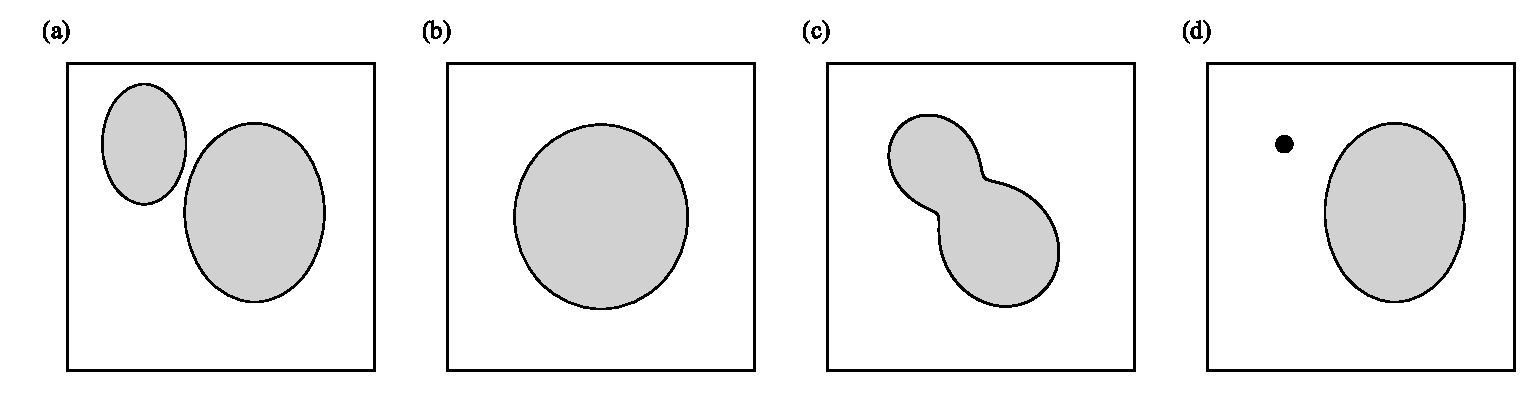
\includegraphics[width=0.72\textwidth]{fig_8.6.pdf}
\caption*{图 8.6\quad (a) 与 (b) 中的两组有向费米面代表两种不同的量子序。(a) 与 (b) 两种量子序之间两个可能的转变点由 (c) 与 (d) 中的费米面描述。}
\end{figure}

\subsection{自由费米系统中的量子序与量子相变}

\begin{keypoints}
\item 自由费米系统包含不改变任何对称性的量子相变，这表明自由费米系统含有非平庸的量子序。
\item 自由费米系统中的不同量子序由费米面的拓扑来分类。
\end{keypoints}

让我们考虑一个只具有平移对称性以及来自费米子数守恒的 $U(1)$ 对称性的自由费米系统。哈密顿量具有如下形式：
\begin{equation*}
H=\sum_{\langle ij\rangle}\left(c_{i}^{\dagger}t_{ij}c_{j}+\text{h.c.}\right)
\end{equation*}
其中 $t_{ij}^{*}=t_{ji}$。基态由在每个负能量态上填充一个费米子得到。一般地，系统含有若干片费米面。

为了理解自由费米子基态中的量子序，我们注意到，当我们连续地改变 $t_{ij}$ 时，费米面的拓扑可以通过两种方式改变：一片费米面可以收缩为零（图 8.6(d)）；两片费米面可以连接起来（图 8.6(c)）。当 $d$ 维系统中的一片费米面即将消失时，基态能量密度具有如下形式：
\begin{equation*}
\rho_{E}=\int\frac{\mathrm{d}^{d}\pmb{k}}{(2\pi)^{d}}\left(\pmb{k}\cdot M\cdot\pmb{k}-\mu\right)\Theta\left(-\pmb{k}\cdot M\cdot\pmb{k}+\mu\right)+\cdots
\end{equation*}
其中"……"代表非奇异的贡献，对称矩阵 $M$ 是正（或负）定的。我们发现基态能量密度在 $\mu=0$ 处具有奇异性，即 $\rho_{E}=c\mu^{(2+d)/2}\Theta(\mu)+\cdots$，其中 $\Theta(x>0)=1$，$\Theta(x<0)=0$。当两片费米面即将连接时，奇异性仍由上式决定，只是此时 $M$ 既有负本征值又有正本征值。基态能量密度在 $d$ 为奇数时具有 $\rho_{E}=c\mu^{(2+d)/2}\Theta(\mu)+\cdots$ 形式的奇异性，在 $d$ 为偶数时具有 $\rho_{E}=c\mu^{(2+d)/2}\log|\mu|+\cdots$ 形式的奇异性。

\begin{figure}[H]
\centering
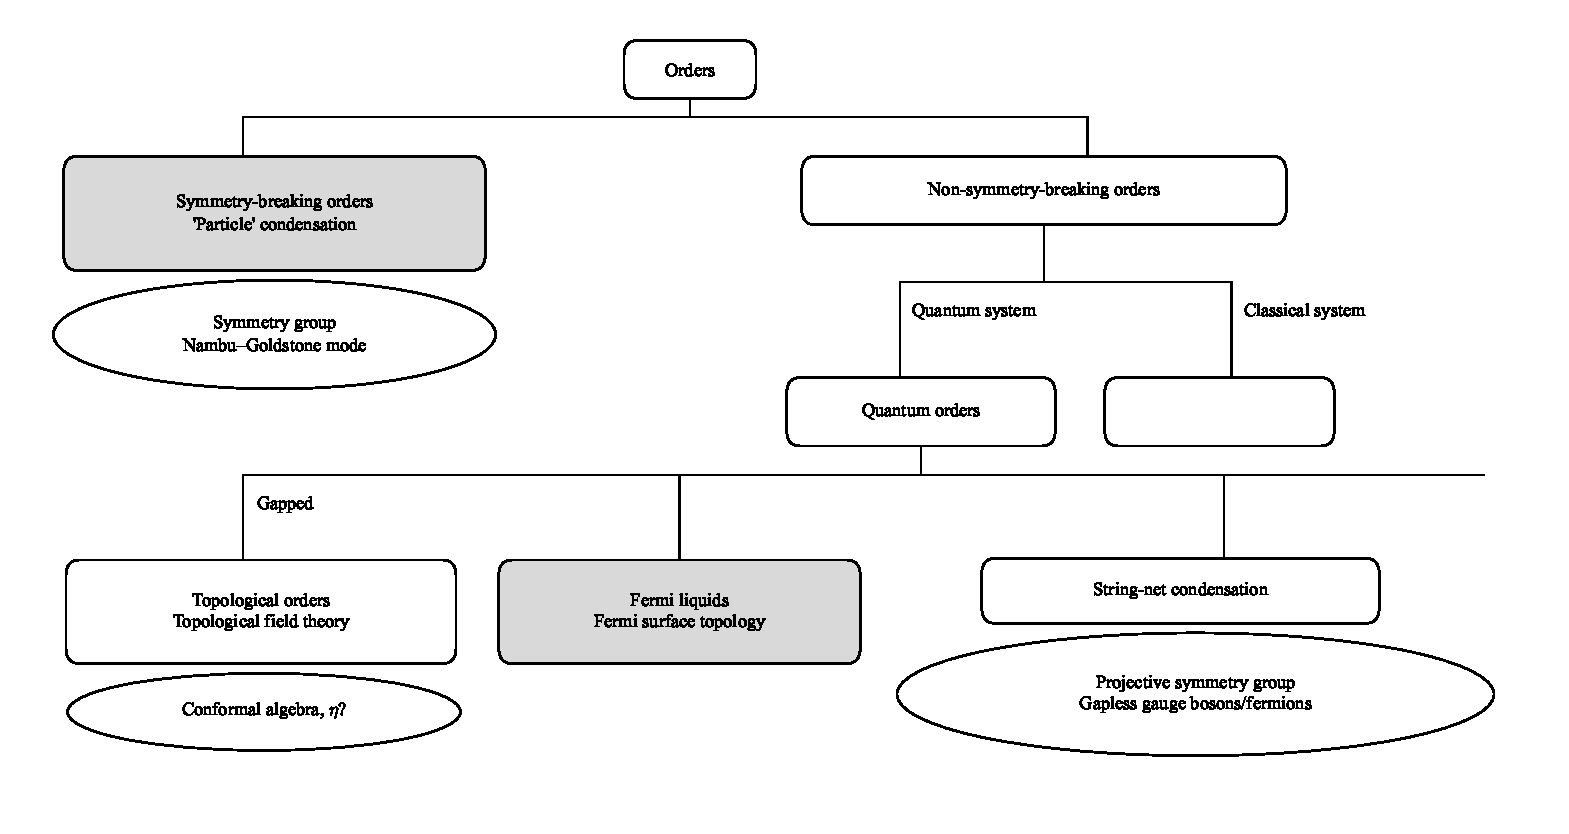
\includegraphics[width=0.72\textwidth]{fig_8.7.pdf}
\caption*{图 8.7\quad 序的一种新分类。阴影框中的相可以用朗道的理论描述，其余的相则超越朗道的理论。}
\end{figure}

基态能量密度在 $\mu=0$ 处的奇异性标志着一次量子相变。这类相变最早由 Lifshitz (1960) 研究。显然，相变两侧没有对称性的改变，也没有局域序参量可以表征相变两侧的相。这表明这两个态只能靠它们的量子序来区分。由于 $\mu=0$ 的位置恰好是费米面拓扑发生改变的地方，我们发现费米面的拓扑是一个刻画自由费米系统中量子序的"量子数"（见图 8.6）。拓扑的改变标志着改变量子序的连续量子相变。

\subsection*{问题 8.3.1}

考虑一个二维自旋-$1/2$ 自由电子系统。当我们改变化学势 $\mu$ 时，系统经历一次量子相变，如图 8.6(d) 所示。试求转变点 $\mu_{c}$ 附近自旋磁化率的奇异行为。

\section{序的一种新分类}

\begin{keypoints}
\item 量子序有许多类。FQH 态和自由费米系统只是众多类量子序中的两类。
\end{keypoints}

拓扑序/量子序的概念使我们能够对序进行一种新的分类，如图 8.7 所示。按照这一分类，量子序就是量子系统中的非对称性破缺序，而拓扑序就是具有有限能隙的量子序。

从上面讨论的 FQH 态和费米液体态可以看到，量子序可以分成若干不同的类。FQH 态和自由费米系统只提供了量子序的两个例子。在接下来几章中，我们将研究某些强关联系统中的量子序。我们将证明，这些量子序属于另外一个类，它与关联基态中弦网的凝聚密切相关。第 9 章将用投影构造（即从属玻色子方法）研究并分类这一类量子序。第 10 章将把第 9 章所研究的量子有序态与弦网凝聚态联系起来。

 % 本文件由 scripts/assemble.py 自动装配，勿手改（改 parts/ 后重跑）
% 第9章 自旋液体与量子序的平均场理论

% 第9章 MEAN-FIELD THEORY OF SPIN LIQUIDS AND QUANTUM ORDER

\chapter{自旋液体与量子序的平均场理论}

\begin{keypoints}
\item 用从属玻色子方法（或投影构造）建立自旋液体态的平均场理论。
\item 规范相互作用的重要性，以及如何应用（含规范相互作用的）平均场理论来研究自旋液体的物理性质。
\item 自旋液体的表征，以及拓扑序与量子序的概念。
\end{keypoints}

在本章中，我们将为自旋液体态建立一个平均场理论。这里所谓"自旋液体态"，是指具有自旋旋转对称性、且每个元胞含\emph{奇数}个电子的绝缘体。通常，每个元胞含奇数个电子的态具有半填充能带，是导体。因此，自旋液体——如果它们存在的话——是非常奇特的态。自旋液体如此奇异，以致许多人根本不相信它们能够存在。事实上，即使到了现在，我们也还不知道有哪个自旋哈密顿量能被证明可以可靠地给出自旋液体基态。

对于那些相信自旋液体存在的人，他们必须接受或相信自旋液体的下列奇特（或者说迷人）的性质。（i）自旋液体中的激发总是携带分数量子数，例如电中性的自旋 $1/2$，这从电子的任何集合出发都不可能得到；有时激发甚至可以携带分数统计。（ii）不同的自旋液体无法靠它们的对称性质来区分；自旋液体是量子有序态的例子。（iii）有能隙自旋液体的基态总是具有拓扑简并，这种简并不能与任何对称性相联系。（iv）自旋液体总是包含某种规范涨落。

在本章中，我们将假定自旋液体确实存在，并为自旋液体建立平均场理论。平均场理论使我们能够理解自旋液体的某些物理性质。在计入重要的平均场涨落之后，我们将证明，某些平均场态对这些涨落是稳定的，因而代表真实的自旋液体态。由于自旋液体是具有非平凡拓扑序/量子序的典型态，我们将以自旋液体为载体来建立量子序的理论。

\section{量子自旋液体态的投影构造}

在这一节中，我们将使用从属玻色子方法（slave-boson approach，或称投影构造（projective construction））（Baskaran et al., 1987; Affleck et al., 1988; Baskaran and Anderson, 1988; Dagotto et al., 1988; Wen and Lee, 1996; Senthil and Fisher, 2000）来构造二维自旋液体。Baskaran 和 Anderson（1988）在从属玻色子方法中发现的规范结构，对我们理解强关联自旋液体起着关键作用。除从属玻色子方法之外，还可以用另一类投影构造——从属费米子方法或 Schwinger 玻色子方法——来构造自旋液体态（Arovas and Auerbach, 1988; Read and Sachdev, 1991; Sachdev and Park, 2002）。由于从属费米子方法只能给出具有有限能隙的自旋液体，这里我们将集中于从属玻色子方法。

\subsection{自旋液体态的平均场理论}

\begin{keypoints}
\item 自旋液体的平均场理论可以由投影构造得到。
\item 平均场理论以及 $\pi$ 通量相的平均场拟设（ansatz）。
\item $a_0(\pmb{i})$ 的规范涨落实施约束条件。
\end{keypoints}

让我们考虑二维正方格子上的 Hubbard 模型（式 (5.5.1)）。在半填充时，Hubbard 模型化为如下的海森堡模型：
\begin{equation*}
H=\sum_{\langle ij\rangle}J_{ij}\,\pmb{S}_i\cdot\pmb{S}_j
\tag{9.1.1}
\end{equation*}

我们想指出，上述自旋 $1/2$ 模型也可以看作一个硬核玻色子（hard-core boson）模型，其中 $|\downarrow\rangle$ 对应空格点，$|\uparrow\rangle$ 对应被一个玻色子占据的格点。上述哈密顿量很难求解，于是我们用平均场近似来理解它的物理性质。在平均场近似中，我们把 $\pmb{S}_i$ 之一换成其量子平均值 $\langle\pmb{S}_i\rangle$，得到如下平均场哈密顿量：
\begin{equation*}
H_{\text{mean}}=\sum_{\langle ij\rangle}J_{ij}\left(\langle\pmb{S}_i\rangle\cdot\pmb{S}_j+\pmb{S}_i\cdot\langle\pmb{S}_j\rangle-\langle\pmb{S}_i\rangle\cdot\langle\pmb{S}_j\rangle\right)
\end{equation*}

平均场哈密顿量 $H_{\text{mean}}$ 容易求解，我们可以得到 $H_{\text{mean}}$ 的基态，即 $|\Phi_{\text{mean}}\rangle$。我们唯一需要做的，是仔细选取 $\langle\pmb{S}_i\rangle$ 的值，使它们满足所谓的自洽方程
\begin{equation*}
\langle\pmb{S}_i\rangle=\langle\Phi_{\text{mean}}|\pmb{S}_i|\Phi_{\text{mean}}\rangle
\end{equation*}

这就是自旋系统的标准平均场方法。

上述标准平均场方法的问题在于，它只能用于研究有序的自旋态，因为我们从一开始就假定了 $\langle\pmb{S}_i\rangle\neq0$。长期以来，自旋液体的平均场理论似乎是不可能建立的。1987 年，我们终于找到了一个奇特的技巧——从属玻色子方法\footnote{从属玻色子（slave boson）和从属费米子（slave fermion）是两个非常奇怪且令人困惑的术语。从属玻色子方法里没有玻色子，从属费米子方法里没有费米子。这就是我更愿意用"投影构造"来称呼这两种方法的原因。}——来做这件事（Baskaran et al., 1987）。为了得到自旋液体的平均场基态，我们引入自旋子（spinon）算符 $f_{i\alpha}$，$\alpha=1,2$，它们是自旋 $1/2$ 的电中性算符。自旋算符 $\pmb{S}_i$ 表示为
\begin{equation*}
\pmb{S}_i=\frac{1}{2}f^{\dagger}_{i\alpha}\sigma_{\alpha\beta}f_{i\beta}
\tag{9.1.2}
\end{equation*}

用自旋子算符表示，哈密顿量 (9.1.1) 可以改写为
\begin{equation*}
H=\sum_{\langle ij\rangle}-\frac{1}{2}J_{ij}f^{\dagger}_{i\alpha}f_{j\alpha}f^{\dagger}_{j\beta}f_{i\beta}+\sum_{\langle ij\rangle}J_{ij}\left(\frac{1}{2}n_i-\frac{1}{4}n_in_j\right)
\tag{9.1.3}
\end{equation*}

这里我们用了 $\sigma_{\alpha\beta}\cdot\sigma_{\alpha'\beta'}=2\delta_{\alpha\beta'}\delta_{\alpha'\beta}-\delta_{\alpha\beta}\delta_{\alpha'\beta'}$，而 $n_i$ 是格点 $i$ 上的费米子数。式 (9.1.3) 中的第二项是常数，在下面的讨论中将略去。注意，式 (9.1.3) 的希尔伯特空间每个格点有四个态，比每格点只有两个态的式 (9.1.1) 的希尔伯特空间要大。式 (9.1.1) 与式 (9.1.3) 之间的等价只在每个格点恰好有一个费米子的子空间中才成立。因此，要用式 (9.1.3) 来描写自旋态，我们需要施加约束（Baskaran et al., 1987; Baskaran and Anderson, 1988）
\begin{equation*}
f^{\dagger}_{i\alpha}f_{i\alpha}=1,\qquad f_{i\alpha}f_{i\beta}\epsilon_{\alpha\beta}=0
\tag{9.1.4}
\end{equation*}

第二个约束实际上是第一个约束的推论。

零阶平均场基态可以通过如下近似得到。首先，我们用约束 (9.1.4) 的基态平均值
\begin{equation*}
\langle f^{\dagger}_{i\alpha}f_{i\alpha}\rangle=1
\tag{9.1.5}
\end{equation*}

来代替约束本身。这一约束可以通过在哈密顿量中引入一个依赖格点且不依赖时间的拉格朗日乘子 $a_0(\pmb{i})(f^{\dagger}_{i\alpha}f_{i\alpha}-1)$ 来实施。其次，我们把算符 $f^{\dagger}_{i\alpha}f_{j\alpha}$ 换成其基态期望值 $\chi_{ij}$，同样忽略它们的涨落。这样，我们便得到零阶平均场哈密顿量
\begin{equation*}
H_{\text{mean}}=\sum_{\langle ij\rangle}-\frac{1}{2}J_{ij}\left[\left(f^{\dagger}_{i\alpha}f_{j\alpha}\chi_{ji}+\text{h.c}\right)-|\chi_{ij}|^{2}\right]+\sum_{i}a_0(\pmb{i})\left(f^{\dagger}_{i\alpha}f_{i\alpha}-1\right)
\tag{9.1.6}
\end{equation*}

式 (9.1.6) 中的 $\chi_{ij}$ 必须满足自洽条件
\begin{equation*}
\chi_{ij}=\langle f^{\dagger}_{i\alpha}f_{j\alpha}\rangle
\tag{9.1.7}
\end{equation*}

而依赖格点的化学势 $a_0(\pmb{i})$ 则选得使平均场基态满足式 (9.1.5)。为方便起见，我们将把 $\chi_{ij}$ 称为自旋液体态的"拟设"。

设 $\bar{\chi}_{ij}$ 是式 (9.1.7) 的一个解，$\bar{a}(\pmb{i})$ 是式 (9.1.5) 的一个解。这样的拟设对应于平均场基态。由于 $\chi_{ij}$ 和 $a_0$ 在自旋旋转变换下不变，平均场基态在自旋旋转变换下不变。如果我们忽略 $\bar{\chi}_{ij}$ 和 $\bar{a}(\pmb{i})$ 的涨落，则平均场态周围的激发由下式描写：
\begin{equation*}
H_{\text{mean}}=\sum_{\langle ij\rangle}-\frac{J_{ij}}{2}\left[\left(f^{\dagger}_{i\alpha}f_{j\alpha}\bar{\chi}_{ji}+\text{h.c}\right)-|\bar{\chi}_{ij}|^{2}\right]+\sum_{i}\bar{a}_0(\pmb{i})\left(f^{\dagger}_{i\alpha}f_{i\alpha}-1\right)
\end{equation*}

我们看到，零阶平均场理论中的激发是由 $f_{i\alpha}$ 描写的自由自旋子。自旋子是自旋 $1/2$ 的中性费米子。令人惊叹的是，费米子激发竟然能从一个纯玻色的模型——式 (9.1.1)——中演生出来。

现在的问题是：我们是否应该相信这个平均场结果？我们是否应该相信具有自旋 $1/2$ 中性费米子激发的自旋液体能够存在？检验的办法之一是把平均场拟设周围的涨落包括进来，看看涨落是否会改变平均场结果。因此，下面我们将考虑涨落的效应。

首先，我们想指出，如果当初把 $a_0$ 的涨落（即时间依赖性）包括进来，约束 (9.1.5) 就会变回原来的约束 (9.1.4)。为看清这一点，让我们考虑 $H_{\text{mean}}$ 的路径积分表述：
\begin{gather*}
Z=\int\mathcal{D}f\,\mathcal{D}[a_0(\pmb{i})]\,\mathcal{D}\chi_{ij}\,\mathrm{e}^{\mathrm{i}\int\mathrm{d}t\,(\mathcal{L}-\sum_{i}a_0(\pmb{i},t)(f^{\dagger}_if_i-1))}\\
\mathcal{L}=\sum_{i}f^{\dagger}_i\mathrm{i}\partial_tf_i-\sum_{\langle ij\rangle}-\frac{1}{2}J_{ij}\left[\left(f^{\dagger}_{i\alpha}f_{j\alpha}\chi_{ji}+\text{h.c}\right)-|\chi_{ij}|^{2}\right]
\tag{9.1.8}
\end{gather*}

我们看到，对依赖时间的 $a_0(\pmb{i},t)$ 作积分将产生一个约束
\begin{equation*}
\prod_{i,t}\delta\left(f^{\dagger}_i(t)f_i(t)-1\right)
\end{equation*}

它在每个格点 $i$、每个时刻 $t$ 都得到实施。我们还注意到，对 $\chi_{ij}(t)$ 作积分将复原原来的哈密顿量 (9.1.3)。因此，式 (9.1.8) 是自旋模型 (9.1.3) 的一个严格表示。$\chi_{ij}$ 和 $a_0(\pmb{i})$ 中的涨落描写平均场基态之上的集体激发。

这里 $\chi_{ij}$ 有两种涨落：振幅涨落和相位涨落。振幅涨落具有有限能隙，在我们的讨论中并不关键。所以这里我们只考虑平均场拟设 $\bar{\chi}_{ij}$ 周围的相位涨落 $a_{ij}$：
\begin{equation*}
\chi_{ij}=\bar{\chi}_{ij}\mathrm{e}^{-\mathrm{i}a_{ij}}
\tag{9.1.9}
\end{equation*}

把上述相位涨落和 $a_0$ 的涨落包括进来后，平均场哈密顿量变为
\begin{equation*}
H=\sum_{\langle ij\rangle}-J_{ij}\left(f^{\dagger}_{i\alpha}f_{j\alpha}\bar{\chi}_{ji}\mathrm{e}^{-\mathrm{i}a_{ji}}+\text{h.c}\right)-\sum_{i}a_0(\pmb{i})\left(f^{\dagger}_{i\alpha}f_{i\alpha}-1\right)
\tag{9.1.10}
\end{equation*}

我们想把式 (9.1.10) 称为一阶平均场哈密顿量。由式 (9.1.10) 可见，$a_0$ 和 $a_{ij}$ 所描写的涨落正是一个 $U(1)$ 格点规范场（见式 (6.4.9)）（Baskaran and Anderson, 1988; Lee and Nagaosa, 1992）。该哈密顿量在规范变换
\begin{equation*}
a_{ij}\rightarrow a_{ij}+\theta_i-\theta_j,\qquad f_i\rightarrow f_i\,\mathrm{e}^{\mathrm{i}\theta_i}.
\tag{9.1.11}
\end{equation*}

之下不变。

因此，在一阶平均场理论中，激发由耦合到 $U(1)$ 规范场的自旋子描写（而非零阶平均场理论中的自由自旋子）。

在通常的平均场理论中，我们对相互作用的哈密顿量作近似以简化问题，希尔伯特空间不因平均场近似而改变。投影构造（或从属玻色子方法）在这一点上非常不同：不仅哈密顿量改变了，希尔伯特空间也改变了。这使得由投影构造得到的平均场结果不仅定量上不正确，而且定性上也不正确。例如，平均场基态 $|\Psi_{\text{mean}}\rangle$（式 (9.1.6) 中 $H_{\text{mean}}$ 的基态）甚至不是一个合法的自旋波函数，因为有些格点上可能没有费米子或有两个费米子。然而，不要放弃。在通常的平均场理论中，我们可以通过把平均场态周围的涨落包括进来，在定量上改进近似。在上面我们看到，在投影构造中，我们可以通过把平均场态周围的规范涨落（$a_0,a_{ij}$）包括进来，在定性上改进近似并复原原来的希尔伯特空间。因此，要想从投影构造得到哪怕是定性的结果，至少把平均场态周围的规范涨落包括进来是至关重要的。换句话说，我们在自旋液体的投影构造中把一个自旋切成了两半；把这两半重新粘合起来，以得到正确的物理结果，是十分重要的。

按照零阶平均场理论，自旋液体中的低能激发是自由自旋子。由上面的讨论我们看到，这样的结果是不正确的。按照一阶平均场理论，自旋子通过规范涨落相互作用。规范相互作用可能会剧烈地改变自旋子的性质。我们稍后将回到这个问题。

\subsection*{问题 9.1.1}

证明式 (9.1.3)。

\subsection{信还是不信}

\begin{keypoints}
\item 一阶平均场理论的解禁闭相导致新一类物质态——量子有序态。
\item 向物理自旋波函数的投影，以及 $U(1)$ 规范结构的含义。
\item 作为纠缠之涨落的演生规范玻色子与费米子。
\end{keypoints}

按照一阶平均场理论，平均场基态周围的涨落由规范场和费米子场描写。别忘了，我们原来的模型只是一个相互作用的纯玻色自旋模型。一个纯玻色的模型怎么会有一个由规范场和费米子场描写的有效理论呢？这简直难以置信。让我们检查一下自己是怎么走到这一步的。我们先把玻色的自旋算符拆成两个费米子算符（自旋子算符）的乘积，然后引入一个规范场把自旋子重新粘合成玻色的自旋。从这个角度看，一阶平均场理论好像只是一个假的理论：规范玻色子和费米子似乎都是假的，到头来我们拥有的只不过是玻色自旋涨落。

然而，我们不应过快地抛弃一阶平均场理论。如果规范场处于禁闭相（见 6.4.3 节），它其实能够复现上述玻色自旋涨落的图像。在禁闭相中，自旋子之间通过线性势相互作用，永远不能在低能下作为准粒子出现；规范玻色子在禁闭相中有很大的能隙，不出现在低能谱中。唯一的低能激发是自旋子对，它们对应于玻色自旋涨落。所以一阶平均场理论也许没有用，但它并没有错。它能够给出与常识一致的图像（尽管绕了很远的弯路）。

另一方面，当规范场处于解禁闭相时，一阶平均场理论也能给出有悖常识的图像。在这种情况下，自旋子和规范玻色子将作为良定义的准粒子出现。问题是：我们相信解禁闭相的图像吗？我们相信从纯玻色模型中能够演生出规范玻色子和费米子吗？显然，上面概述的投影构造太过形式化，很难让大多数人相信如此激进的结果。

我不得不说，把自旋切成两半再粘回去这套做法让很多人望而却步。很难看出这种形式操作能带来什么新的物理洞见和结果。如果这条路径真的给出了什么新结果，许多人也会把它们归咎于这一奇怪构造的人为假象，而不是自旋液体的真实物理性质。的确，投影构造非常形式化，但它也是一件超越时代的礼物。我们现在知道，投影构造真正所做的，是产生一个弦网凝聚态。弦网凝聚（string-net condensation）给出一种新型的关联态，它具有非平凡的量子序（见第 10 章）。所以，请相信我：只要恰当地计入规范涨落的效应，投影构造给出的惊人结果是可以信赖的。

这里让我们暂且不用弦网凝聚的图像，试着理解投影构造背后的物理图像。首先，我们需要理解平均场拟设 $\chi_{ij}$ 是如何与每个格点恰好有一个费米子的物理自旋波函数相联系的。我们知道，平均场波态 $|\Psi^{(\chi_{ij})}_{\text{mean}}\rangle$（$H_{\text{mean}}$ 的基态）不是自旋系统的合法波函数，因为它未必每格点有一个费米子。为了把它联系到物理自旋波函数，我们需要把 $a_0$ 的涨落包括进来，以实施每格点一个费米子的约束。有了这一理解，我们就可以把平均场态投影到每格点一个费米子的子空间上，得到自旋系统的一个合法波函数 $\Psi_{\text{spin}}(\{\alpha_i\})$：
\begin{equation*}
\Psi^{(\chi_{ij})}_{\text{spin}}(\{\alpha_i\})=\langle 0_f|\prod_{i}f_{i\alpha_i}|\Psi^{(\chi_{ij})}_{\text{mean}}\rangle.
\tag{9.1.12}
\end{equation*}

其中 $|0_f\rangle$ 是没有 f 费米子的态，即 $f_{i\alpha}|0_f\rangle=0$。式 (9.1.12) 把平均场拟设（连同它的涨落）与物理自旋波函数联系起来，使我们能够理解平均场拟设和平均场涨落的物理意义。

例如，投影 (9.1.12) 赋予规范变换 (9.1.11) 以物理意义。由规范变换
\begin{equation*}
\tilde{\chi}_{ij}=\mathrm{e}^{\mathrm{i}\theta_i}\chi_{ij}\mathrm{e}^{-\mathrm{i}\theta_j}
\tag{9.1.13}
\end{equation*}

联系的两个平均场拟设 $\chi_{ij}$ 与 $\tilde{\chi}_{ij}$ 给出同一个投影后的自旋态
\begin{equation*}
\Psi^{(\tilde{\chi}_{ij})}_{\text{spin}}(\{\alpha_i\})=\mathrm{e}^{\mathrm{i}\sum_i\theta_i}\Psi^{(\chi_{ij})}_{\text{spin}}(\{\alpha_i\})
\tag{9.1.14}
\end{equation*}

对于 $\chi_{ij}$ 的不同取值，式 (9.1.6) 中 $H_{\text{mean}}$ 的基态对应于不同的平均场波函数 $|\Psi^{(\chi_{ij})}_{\text{mean}}\rangle$；投影之后，它们给出不同的物理自旋波函数 $\Psi^{(\tilde{\chi}_{ij})}_{\text{spin}}(\{\alpha_i\})$。因此，我们可以把 $\chi_{ij}$ 看作标记不同物理自旋态的标签。式 (9.1.14) 告诉我们，这个标签不是一对一的，而是多对一的。这一性质对我们理解 $\chi_{ij}$ 涨落的反常动力学性质十分重要。用多个标签标记同一个物理态，也使我们的理论按照 6.1.1 节中的定义成为一门规范理论。

让我们考虑多对一性质，或者说 $\chi_{ij}$ 的规范结构，如何影响它的动力学性质。如果 $\chi_{ij}$ 是物理态的一对一标签，那它就会像玻色超流体中的凝聚玻色子振幅 $\langle\phi(\pmb{x},t)\rangle$，或 SDW 态中的凝聚自旋矩 $\langle\pmb{S}_i(t)\rangle$ 一样，而 $\chi_{ij}$ 的涨落将对应于一种类似自旋波模式的玻色型模式。\footnote{更确切地说，自旋波模式对应于标量玻色子。局域序参量的涨落总是给出标量玻色子。}然而，$\chi_{ij}$ 的行为并不像局域序参量 $\langle\phi(\pmb{x},t)\rangle$ 和 $\langle\pmb{S}_i(t)\rangle$ 那样无冗余地标记物理态。作为多对一的标签，$\chi_{ij}$ 的某些涨落不改变物理态，因而是非物理的；这些涨落被称为纯规范涨落（pure gauge fluctuations）。对一个一般的涨落 $\delta\chi_{ij}$，其中一部分是物理的，另一部分是非物理的。$\chi_{ij}$ 的有效理论必须是规范不变的。这一点剧烈地改变了涨落的动力学性质。正是这一性质使 $\chi_{ij}$ 的涨落表现得像规范玻色子，与声模式和自旋波模式大不相同。

我们已经论证过，$\chi_{ij}$ 的相位涨落对应于规范涨落。投影构造 (9.1.12) 使我们能够得到与规范涨落 $a_{ij}$ 相应的物理自旋波函数：
\begin{equation*}
\Psi^{(a_{ij})}_{\text{spin}}=\langle 0|\prod_{i}f_{i\alpha_i}|\Psi^{(\bar{\chi}_{ij}\mathrm{e}^{\mathrm{i}a_{ij}})}_{\text{mean}}\rangle.
\end{equation*}

类似地，投影构造也使我们能够得到与一对自旋子激发相应的物理自旋波函数。我们从带有一对粒子–空穴激发的平均场基态出发，经过投影 (9.1.12)，便得到含有一对自旋子的物理自旋波函数：
\begin{equation*}
\Psi^{\text{spinon}}_{\text{spin}}(\pmb{i}_1,\alpha_1;\pmb{i}_2,\alpha_2)=\langle 0|\Big(\prod_{i}f_{i\alpha_i}\Big)f^{\dagger}_{\pmb{i}_1\lambda_1}f_{\pmb{i}_2\lambda_2}|\Psi^{(\bar{\chi}_{ij})}_{\text{mean}}\rangle.
\end{equation*}

如果你对这里给出的物理图像不满意，仍然不相信投影构造能够产生演生的规范玻色子和费米子，那么你可以直接跳到第 10 章。在第 10 章中，我们构造了几个能够用投影构造精确（或准精确）求解的自旋模型。这些模型具有演生的 $Z_2/U(1)$ 规范结构和费米子。这些精确可解模型揭示了演生规范玻色子和费米子的弦网起源。在本章其余部分，我们假定投影构造是有意义的，并研究它的推论。

\begin{figure}[H]
\centering
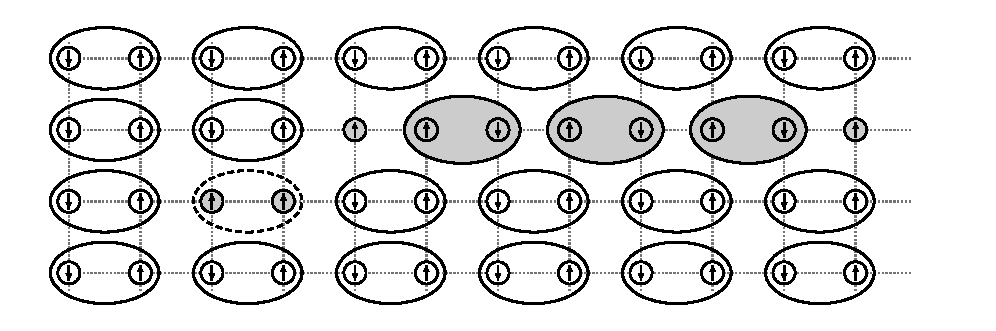
\includegraphics[width=0.72\textwidth]{fig_9.1.pdf}
\caption*{图 9.1\quad 二聚体态由自旋单态对构成。把一个二聚体变成三重态便产生一个自旋 1 激发。两个分离开的自旋 $1/2$ 激发由一条由错位二聚体构成的弦相连。}
\end{figure}

\subsection{二聚体态}

\begin{keypoints}
\item 二聚体态的一阶平均场理论具有禁闭型的 $U(1)$ 规范相互作用。物理激发中只出现自旋子对的束缚态。
\end{keypoints}

让我们先讨论一个具体的平均场基态——具有最近邻耦合的海森堡模型中的二聚体态（dimer state）（Majumdar and Ghosh, 1969; Affleck et al., 1987; Read and Sachdev, 1989）：
\begin{equation*}
H=J_1\sum_{i}\left(\pmb{S}_i\pmb{S}_{\pmb{i}+\pmb{x}}+\pmb{S}_i\pmb{S}_{\pmb{i}+\pmb{y}}\right).
\tag{9.1.15}
\end{equation*}

二聚体态由如下拟设描写：
\begin{equation*}
\begin{array}{l}
\chi_{i,i+\pmb{x}}=\dfrac{1}{2}\left(1+(-)^{i_x}\right)\\[6pt]
\text{其余}\;=0
\end{array}
\tag{9.1.16}
\end{equation*}

以及 $a_0(\pmb{i})=0$。可以验证，式 (9.1.6) 中 $H_{\text{mean}}$ 的平均场基态满足自洽方程 (9.1.7) 和约束 (9.1.5)。在平均场二聚体态中，自旋子能谱没有色散：
\begin{equation*}
E_k=\pm\frac{1}{2}J_1
\tag{9.1.17}
\end{equation*}

具有 $E_k=-\frac{1}{2}J_1$ 的价带被自旋子完全填满。自旋激发在二聚体态中有有限能隙。同样清楚的是，二聚体态破坏 $x$ 方向的平移对称性。

在零阶平均场理论中，二聚体基态之上的激发是自旋 $1/2$ 的自旋子。这一结果显然不对，因为从物理上看，二聚体态是由填满格子的自旋单态二聚体构成的（见图 9.1），基本激发对应于自旋三重态的二聚体，即玻色型的自旋 1 激发。在一阶平均场理论中，自旋子耦合到 $U(1)$ 规范场。在 $2+1$ 维，$U(1)$ 规范理论是禁闭的，因此单个自旋子不可观测，物理谱中只能出现玻色型的束缚态（携带整数自旋）。如果我们真的制造出两个分离开的自旋 $1/2$ 激发，那么由图 9.1 可见，它们将由一条错位二聚体构成的弦连接起来。这根弦在两个自旋 $1/2$ 激发之间导致线性禁闭相互作用，与一阶平均场理论给出的图像一致。我们看到，一阶平均场理论给出了定性上正确的结果。

\begin{figure}[H]
\centering
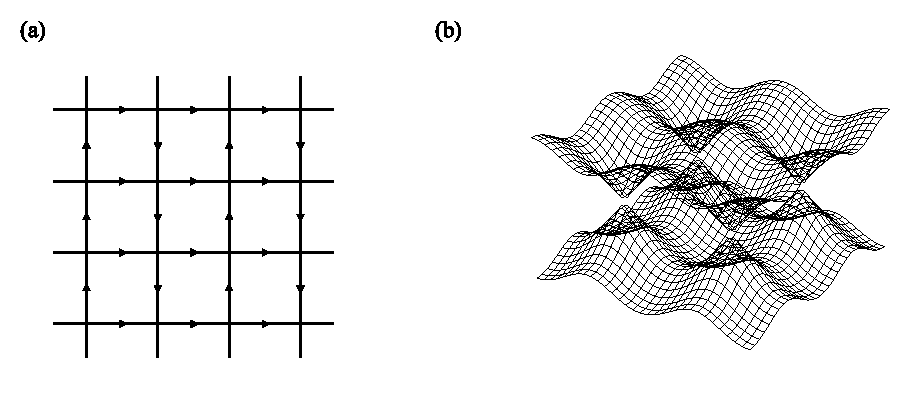
\includegraphics[width=0.72\textwidth]{fig_9.2.pdf}
\caption*{图 9.2\quad (a) $\pi$ 通量态的平均场拟设。沿箭头方向 $\chi_{ij}=\mathrm{i}\chi_1$。(b) $\pi$ 通量态中费米子的色散。价带是填满的。低能激发存在于价带与导带相切的四个费米点附近。}
\end{figure}

\subsection{$\pi$ 通量态}

\begin{keypoints}
\item 投影之后，平均场 $\pi$ 通量相给出平移、旋转和宇称对称的自旋液体波函数。
\item $\pi$ 通量相的低能有效理论（一阶平均场理论）包含无能隙狄拉克费米子耦合到 $U(1)$ 规范场。这些狄拉克费米子携带自旋 $1/2$ 且电中性。
\item 稳定、边缘和不稳定平均场态的概念。
\item 一阶平均场理论只对稳定平均场态或涨落微弱的边缘平均场态可靠。$\pi$ 通量相不是这些平均场态之一。
\end{keypoints}

我们要研究的第二个平均场态，是最近邻海森堡模型的 $\pi$ 通量态（$\pi$-flux state）（Affleck and Marston, 1988; Kotliar, 1988）。$\pi$ 通量态由如下拟设给出（见图 9.2）：
\begin{equation*}
\chi_{i,i+\pmb{x}}=\mathrm{i}\chi_1,\qquad \chi_{i,i+\pmb{y}}=\mathrm{i}\chi_1(-)^{i_x},\qquad a_0(\pmb{i})=0.
\tag{9.1.18}
\end{equation*}

平均场哈密顿量 (9.1.6) 等价于每个方格带 $\pi$ 通量的电子跳跃问题，因为绕一个方格一周有 $\prod\chi_{ij}\propto\mathrm{e}^{\mathrm{i}\pi}$。$\pi$ 通量相中自旋子能谱为（见图 9.2）
\begin{equation*}
E_k=\pm J_1\chi_1\sqrt{\sin(k_x)^{2}+\sin(k_y)^{2}}
\tag{9.1.19}
\end{equation*}

其中 $-\frac{\pi}{2}<k_x<\frac{\pi}{2}$，$-\pi<k_y<\pi$。$\chi_1$ 的值可以由对平均场能量
\begin{equation*}
-\sum_{\pmb{k}}^{\prime}J_1\chi_1\sqrt{\sin(k_x)^{2}+\sin(k_y)^{2}}+J_1|\chi_1|^{2}N_{\text{site}}
\end{equation*}

求极小得到。我们发现
\begin{equation*}
\chi_1=\frac{1}{4}\int\frac{\mathrm{d}^{2}\pmb{k}}{(2\pi)^{2}}\sqrt{\sin(k_x)^{2}+\sin(k_y)^{2}}
\end{equation*}

除 $\pi$ 通量相之外，还有许多其他不同的平均场拟设局部地使平均场能量取极小。不过，对于只有最近邻耦合 $J_1$ 的海森堡模型，$\pi$ 通量相在平移不变的自旋液体中平均场能量最低。

让我们讨论 $\pi$ 通量相的一些物理性质。首先，考虑平均场态的对称性。我们知道，平均场理论旨在描写一个自旋态，其波函数为 $\Psi_{\text{spin}}(\{\alpha_i\})$，其中 $\alpha_i=\pm 1/2$ 是格点 $i$ 上 $S^{z}$ 的取值。当我们说"平均场态的对称性"时，我们真正指的是"相应自旋波函数 $\Psi_{\text{spin}}(\{\alpha_i\})$ 的对称性"。相应的自旋波函数由平均场态投影到每格点一个费米子的子空间得到（见式 (9.1.12)）。

由于平均场拟设 $\chi_{ij}$ 不依赖自旋取向，平均场基态中每一个负能级都被一个自旋向上和一个自旋向下的费米子占据。因此，平均场态 $|\Psi^{(\chi_{ij})}_{\text{mean}}\rangle$ 在自旋旋转下不变；结果，投影得到的物理自旋波函数也在自旋旋转下不变。

然而，平均场拟设在沿 $x$ 方向平移一个晶格间距下并非不变。因此，平均场态 $|\Psi^{(\chi_{ij})}_{\text{mean}}\rangle$ 破坏平移对称性。这似乎暗示物理自旋波函数也破坏平移对称性。事实上，物理自旋波函数并不破坏平移对称性。原因在于，平移后的拟设 $(\chi_{i,i+\pmb{x}},\chi_{i,i+\pmb{y}})=(-\mathrm{i}\chi_1(-)^{i_x},\mathrm{i}\chi_1)$ 通过取 $\mathrm{e}^{\mathrm{i}\theta_i}=(-)^{i_x}$ 的规范变换 (9.1.11) 与原拟设 $(\chi_{i,i+\pmb{x}},\chi_{i,i+\pmb{y}})=(\mathrm{i}\chi_1(-)^{i_x},\mathrm{i}\chi_1)$ 相联系。因此，这两个拟设给出同一个物理自旋波函数，投影后的自旋波函数在平移下不变。$\pi$ 通量相是一个平移对称的自旋液体。

第二，我们考虑低能激发的性质。半填充（即平均每格点一个费米子）时的费米面是位于 $(k_x,k_y)=(0,0)$ 和 $(0,\pi)$ 的点。在平均场层次上，$\pi$ 通量态含有无能隙自旋激发，它们对应于跨费米点的粒子–空穴激发。除这些无能隙自旋激发之外，平均场通量态还含有 $U(1)$ 规范涨落 $(a_{ij},a_0)$。在一阶平均场理论中，低能激发由耦合到 $U(1)$ 规范场的无能隙自旋子描写。

如果我们忽略自旋子 $f_i$ 与规范涨落 $(a_{ij},a_0)$ 之间的相互作用，那么 $\pi$ 通量相将具有由费米型准粒子描写的无能隙中性自旋 $1/2$ 激发。然而，除非证明了在计入规范相互作用后这一结果仍然成立，我们不应相信这个惊人的结果。

现在让我们考虑自旋激发与规范涨落之间的相互作用。为方便起见，让我们在哈密顿量 (9.1.10) 中加上 Maxwell 项 $\frac{1}{8\pi g^{2}}(v^{2}f_{12}^{2}-f_{0i}^{2})$，其中 $g$ 是耦合常数，$f_{\mu\nu}$ 是 $a_{\mu}$ 的场强。原理论对应于 $g\to\infty$ 的极限。Maxwell 项是在积掉费米子的过程中产生的。设 $g(\Lambda)$ 是积掉能标 $\Lambda$ 与 $\Lambda_0$ 之间的费米子后得到的耦合常数，其中 $\Lambda_0$ 是原理论中的能量截断。由量纲分析可得 $\mathrm{d}g^{-2}(\Lambda)\sim\mathrm{d}\Lambda/\Lambda^{2}$（注意 $\mathrm{d}g^{-2}(\Lambda)\propto\mathrm{d}\Lambda$）。于是 $g^{-2}(\Lambda)\sim\Lambda^{-1}-\Lambda_0^{-1}$。

由于与规范场耦合，一个自旋子会产生规范场 $(a_0,a_{ij})$ 的"电"场 $f_{0i}$（注意自旋子携带规范场的一个单位电荷）。粒子–空穴激发中粒子–空穴对之间的势能为
\begin{equation*}
V(\pmb{r}_1-\pmb{r}_2)=2\pi g^{2}\ln|\pmb{r}_1-\pmb{r}_2|
\tag{9.1.20}
\end{equation*}

我们发现粒子与空穴在长距离上仍有相互作用。为估计这一相互作用的强度和效应，让我们比较粒子–空穴对的动能 $E_K\sim 1/|\pmb{r}_1-\pmb{r}_2|$ 与势能 $V(\pmb{r}_1-\pmb{r}_2)$。由于 $g^{2}\sim v/|\pmb{r}_1-\pmb{r}_2|$（假定 $\Lambda\sim v/|\pmb{r}_1-\pmb{r}_2|$），我们看到 $V/E_K\sim 1$。这意味着相互作用是边缘的，在低能下不能忽略。这一结果提示，$\pi$ 通量态中的量子涨落（例如规范涨落）是重要的，将剧烈改变零阶平均场理论的低能性质。在这种情况下，零阶平均场理论（具有自由自旋子激发）不能给出自旋液体低能性质的可靠图像。要得到 $\pi$ 通量态可靠的低能性质，必须处理无能隙费米子与规范场的耦合系统。忽略规范相互作用而得到的那些惊人性质可能并不成立。\footnote{当平均场涨落微弱时，边缘平均场态可以导致代数自旋液体（algebraic spin liquid）——一种在低能下没有自由准粒子的自旋液体。见 9.9.5 节和 9.10 节。}

我们看到，投影构造的怀疑者们是对的：零阶平均场理论的结果有误导性，不可轻信。然而，相信者们也是对的：一阶平均场理论确实告诉我们，零阶平均场理论的结果是不正确的。到目前为止，投影构造没有误导过我们；只要计入适当的涨落，它是可以信赖的。与自旋液体物理性质相对应的，是一阶平均场理论（而非零阶平均场理论）的结果。

为了刻画平均场态周围涨落的重要性，这里我们想引入稳定、边缘和不稳定平均场态三个概念。在稳定平均场态中，涨落是微弱的，涨落诱导的相互作用在低能下消失（即相互作用是不相关微扰）。在边缘平均场态中，相互作用与能量之比在低能极限下趋于有限常数，此时相互作用是边缘微扰。在不稳定平均场态中，相互作用与能量之比在低能极限下发散，此时相互作用是相关微扰。只有对稳定平均场态，零阶平均场理论的性质才能在涨落之下幸存。对于不稳定平均场态，涨落会在低能下驱动相变，我们无法从零阶平均场理论推出自旋液体的任何物理性质。在这种情况下，一阶平均场理论也没有用，因为它并不能帮助我们推出自旋系统的物理性质。上面讨论的 $\pi$ 通量态是一个边缘平均场态。对于边缘平均场态，如果相互作用与能量之比很小，一阶平均场理论可能有用；此时相应自旋态的物理性质可以微扰地计算。对 $\pi$ 通量态而言，相互作用与能量之比是 1 的量级，因此很难从一阶平均场理论得到 $\pi$ 通量态的低能物理性质。

由上述讨论可见，一阶平均场理论只对稳定平均场态以及涨落微弱的边缘平均场态有用。用平均场理论研究自旋液体的关键，在于找到稳定平均场态（见 9.1.6、9.2.4 和 9.2.6 节），或涨落微弱的边缘平均场态（见 9.8 节）。

\subsection*{问题 9.1.2}

$\pi$ 通量态的旋转对称性

\begin{enumerate}
\item 证明式 (9.1.14)。
\item 证明 $\pi$ 通量态不破坏 $90^{\circ}$ 旋转对称性。
\end{enumerate}

% 块边界判定：
%   起点——书页 367（p382）顶部为 Problem 9.1.3，新起条目，无 ch9_a 溢出内容，
%     故本块无 %JOIN%，也不设 %--A-TAIL-- 区（ch9_a 止于书页 366 末的问题 9.1.2）。
%   终点——书页 379（p394）止于 9.2.2 节首要点列表的前两条；第三条要点印在
%     书页 380（p395）顶部，连同其后的正文 "Just like the U(1) ..." 均属 ch9_c。
%     本块按"要点列表只收到本页末"处理：keypoints 环境在两条后闭合；
%     第三条的原文与建议译文见文件尾【块界备注】，请 ch9_c 以其文件的
%     %--B-TAIL-- 区或正文开头续排该条（环境需另行开启），勿弃勿重。

\subsection*{问题 9.1.3}

设 $|\Psi_{\text{mean}}\rangle$ 为 $\pi$ 通量拟设的平均场基态。计算 $\langle\Psi_{\text{mean}}|\pmb{S}_i\pmb{S}_{i+\pmb{y}}|\Psi_{\text{mean}}\rangle$。利用这一结果求变分平均场能量 $\langle\Psi_{\text{mean}}|H|\Psi_{\text{mean}}\rangle$，其中 $H$ 是具有近邻相互作用的海森堡模型（见式 (9.1.15)）。比较 $\pi$ 通量态与二聚体态的平均场能量。

\subsection*{问题 9.1.4}

\textbf{Dirac 费米子}

\begin{enumerate}
\item 证明：在连续极限下，$\pi$ 通量态中的低能自旋子由下式描述
\begin{equation*}
H=v\sum_{\pmb{k}\sim0}\lambda^{\dagger}_{\alpha,\pmb{k}}(k_x\Gamma_x+k_y\Gamma_y)\lambda_{\alpha,\pmb{k}}
\end{equation*}
其中 $\lambda^{\top}_{\alpha,\pmb{k}}=(f_{\alpha,\pmb{k}},f_{\alpha,\pmb{k}+\pmb{Q}})$，$\pmb{Q}=(\pi,\pi)$，且 $\Gamma_x^2=\Gamma_y^2=1$。求 $v$ 与 $\Gamma_{x,y}$。在实空间中，$H$ 可改写为 $H=\int\mathrm{d}^2x\,v\lambda^{\dagger}_{\alpha}(-\mathrm{i}\Gamma_x\partial_x-\mathrm{i}\Gamma_y\partial_y)\lambda_{\alpha}$。

\item 相应的拉格朗日量 $\mathcal{L}=\mathrm{i}\lambda^{\dagger}_{\alpha}\partial_t\lambda_{\alpha}-v\lambda^{\dagger}_{\alpha}(-\mathrm{i}\Gamma_x\partial_x-\mathrm{i}\Gamma_y\partial_y)\lambda_{\alpha}$ 可以改写为
\begin{equation*}
\mathcal{L}=\mathrm{i}\bar{\lambda}_{\alpha}(\gamma^0\partial_t+v\gamma^x\partial_x+v\gamma^y\partial_y)\lambda_{\alpha}
\end{equation*}
其中 $\bar{\lambda}_{\alpha}=\lambda^{\dagger}_{\alpha}\gamma^0$，$\gamma_0^2=1$，且 $(\Gamma_x,\Gamma_y)=(-\gamma^0\gamma^x,-\gamma^0\gamma^y)$。求 $\gamma^{0,x,y}$。由 $\mathcal{L}$ 描述的费米子称为无质量狄拉克费米子。

\item 证明 $(\gamma^0,\gamma^x,\gamma^y)$ 在 $1+2$ 维中满足下列狄拉克代数：
\begin{equation*}
\{\gamma^{\mu},\gamma^{\nu}\}=\eta^{\mu\nu},\qquad \mu,\nu=0,x,y,
\end{equation*}
其中 $\eta^{\mu\nu}$ 是对角矩阵，$\eta^{00}=1$ 且 $\eta^{xx}=\eta^{yy}=-1$。

\item 有质量的狄拉克费米子由如下拉格朗日量描述：
\begin{equation*}
\mathcal{L}=\mathrm{i}\bar{\lambda}_{\alpha}(\gamma^0\partial_t+v\gamma^x\partial_x+v\gamma^y\partial_y)\lambda_{\alpha}+m\bar{\lambda}_{\alpha}\lambda_{\alpha}.
\end{equation*}
求相应运动方程 $\mathrm{i}(\gamma^0\partial_t+v\gamma^x\partial_x+v\gamma^y\partial_y+m)\lambda_{\alpha}=0$ 的解。证明该费米子具有色散 $\omega_{\pmb{k}}=\sqrt{v^2\pmb{k}^2+m^2}$。

\item \emph{与 $U(1)$ 规范场的耦合}

用 3.7.1 节所述的程序，求最小耦合到一个 $U(1)$ 规范场的狄拉克费米子的拉格朗日量。确保所得的拉格朗日量具有 $U(1)$ 规范不变性。
\end{enumerate}

\subsection{如何消除无能隙 $U(1)$ 规范玻色子}

\begin{keypoints}
\item 如何得到稳定的平均场态：通过 Chern--Simons 项和/或 Anderson--Higgs 机制让规范涨落获得有限能隙。
\item 稳定的自旋液体总包含电中性的自旋 $1/2$ 自旋子，且自旋子之间只有短程相互作用。
\end{keypoints}

我们已经看到，在 $\pi$ 通量态中，无能隙 $U(1)$ 规范玻色子与无能隙费米子强烈相互作用，甚至直到零能。对于 $\pi$ 通量相，很难求出一阶平均场理论（即费米子--规范场耦合系统）的性质。一阶平均场理论虽然不会误导我们，但它似乎复杂得毫无用处。现在的问题是：能否构造一个稳定的平均场态，使平均场涨落在低能下相互作用微弱？如果可以，一阶平均场理论的性质就能容易地求得。

由于一阶平均场理论至少必须包含实施每格点单费米子约束的规范涨落，得到稳定平均场态的一个办法是让规范玻色子获得能隙。有能隙的规范玻色子只能传递费米子之间的短程相互作用。基于朗道费米液体理论的经验，我们知道如何处理具有短程相互作用的费米子。

首先让我们澄清"让规范玻色子获得能隙"是什么意思。我们知道，规范玻色子不过是平均场拟设 $\chi_{ij}$ 的涨落。这些涨落的动力学依赖于平均场拟设。因此，所谓"让规范玻色子获得能隙"，指的就是找到这样的平均场拟设，使拟设的集体模式涨落有能隙。

为给寻找稳定平均场拟设的探索提供动机，让我们先考虑 $U(1)$ 规范玻色子可以通过哪些方式获得能隙。事实上，在 3.7.5 节和 4.4 节中，我们已经遇到过 $U(1)$ 规范玻色子获得能隙的两种方式。第一种方式是 Anderson--Higgs 机制（Anderson--Higgs mechanism），即规范玻色子与凝聚的电荷玻色子耦合。耦合系统的动力学由
\begin{equation*}
\mathcal{L}=\frac{1}{8\pi g^2}(\mathbf{e}^2-b^2)+c_1a_0^2-c_2\pmb{a}^2
\end{equation*}
在 $2+1$ 维及连续极限下描述（见式 (3.7.17)），其中 $c_1$ 与 $c_2$ 来自凝聚的电荷玻色子。第二种方式是通过 Chern--Simons 项。如果平均场拟设使得满带具有非零的霍尔电导，那么 $U(1)$ 规范玻色子的动力学将由
\begin{equation*}
\mathcal{L}=\frac{1}{8\pi g^2}(\mathbf{e}^2-b^2)+\frac{K}{4\pi}\epsilon^{\mu\nu\lambda}a_{\mu}\partial_{\nu}a_{\lambda}.
\tag{9.1.21}
\end{equation*}
描述。在问题 9.1.5 中我们将求出，Chern--Simons 项给规范玻色子一个非零能隙。找到稳定平均场态的关键，在于找到实现上述两种机制之一的平均场拟设。

在这两种情形中，规范场都只能传递短程相互作用。其结果是，自旋子不被禁闭。自旋液体之上的准粒子由自由自旋子描述，它们携带自旋 $1/2$、电荷为零。在存在 Chern--Simons 项时，自旋子甚至可以具有分数统计。

\begin{figure}[H]
\centering
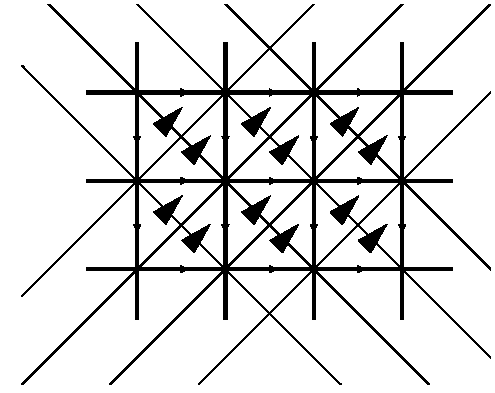
\includegraphics[width=0.72\textwidth]{fig_9.3.pdf}
\caption*{图 9.3\quad 手征自旋态的平均场拟设。$\chi_{ij}$ 在箭头方向上为 $\mathrm{i}\chi$。}
\end{figure}

\subsection*{问题 9.1.5}

证明由式 (9.1.21) 描述的涨落具有有限能隙。（可以通过计算经典运动方程来做到这一点。）

\subsection{手征自旋态}

\begin{keypoints}
\item 平均场手征自旋拟设给出一个平移和旋转对称的自旋液体态，但它破坏时间反演与宇称对称性。
\item 平均场手征自旋态是稳定的。由平均场理论得到的手征自旋液体确实代表真实自旋系统的一个稳定量子相。
\item 手征自旋液体含有分数化激发——自旋子。自旋子携带自旋 $1/2$、不带电荷，并具有分数统计。
\end{keypoints}

在这一节中，我们将讨论实现上述第二种机制的一个平均场态。该平均场态由拟设 $\chi_{ij}$ 描述，其中 $\chi_{ij}$ 是复数并产生通量。由式 (9.1.6) 描述的自旋子的行为就好像在磁场中运动。当通量与自旋子密度（即每格点一个费米子）有正确的公度关系（commensuration）时，整数个朗道能级（更确切地说，由于晶格的存在，是朗道能带）被完全填满。在这种情况下，有效格点规范理论因填满的朗道能级的有限霍尔电导而含有一个 Chern--Simons 项。我们将把这样的稳定平均场态称为手征自旋态（chiral spin state）（Wen et al., 1989; Khveshchenko and Wiegmann, 1989）。

最简单的手征自旋态由下列拟设给出（见图 9.3）：
\begin{equation*}
\begin{array}{lll}
\chi_{i,i+\pmb{x}}=\mathrm{i}\chi_1, & \chi_{i,i+\pmb{y}}=\mathrm{i}\chi_1(-)^{i_x}, & a_0(i)=0,\\[2pt]
\chi_{i,i+\pmb{x}+\pmb{y}}=-\mathrm{i}\chi_2(-)^{i_x}, & \chi_{i,i+\pmb{x}-\pmb{y}}=\mathrm{i}\chi_2(-)^{i_x} &
\end{array}
\tag{9.1.22}
\end{equation*}

上述 $\chi_{ij}$ 在每个正方形中产生 $\pi$ 通量，在每个三角形中产生 $\frac{1}{2}\pi$ 通量。上一节讨论的 $\pi$ 通量相有些特殊：由于 $\pi$ 通量等价于 $-\pi$ 通量，$\pi$ 通量相保持时间反演对称性（$T$）与宇称（$P$）。然而，由式 (9.1.22) 描述的 $\frac{1}{2}\pi$ 通量相并不等价于 $-\frac{1}{2}\pi$ 通量相。在 $T$ 或 $P$ 之下，$\frac{1}{2}\pi$ 通量变为 $-\frac{1}{2}\pi$ 通量，式 (9.1.22) 中的 $\chi_2$ 变为 $-\chi_2$。因此，具有非零 $\chi_2$ 的手征自旋态自发破坏 $T$ 与 $P$。利用恒等式
\begin{equation*}
E_{123}\equiv\pmb{S}_1\cdot(\pmb{S}_2\times\pmb{S}_3)=2\mathrm{i}(\hat{\chi}_{12}\hat{\chi}_{23}\hat{\chi}_{31}-\hat{\chi}_{13}\hat{\chi}_{32}\hat{\chi}_{21}),\qquad \hat{\chi}_{ij}=f^{\dagger}_if_j
\tag{9.1.23}
\end{equation*}
我们发现 $\langle E_{123}\rangle\sim\mathrm{Im}(\chi_{12}\chi_{23}\chi_{31})$ 在手征自旋态中不为零。注意 $E_{123}$ 在 $T$ 或 $P$ 下为奇；因此可以把 $E_{123}$ 视为 $T$ 与 $P$ 破坏的序参量。

指定了手征自旋态之后，我们想知道哪个自旋哈密顿量支持手征自旋态。让我们考虑下列阻挫自旋哈密顿量：
\begin{equation*}
H=J_1\sum_i(\pmb{S}_i\cdot\pmb{S}_{i+\pmb{x}}+\pmb{S}_i\cdot\pmb{S}_{i+\pmb{y}})+J_2\sum_i(\pmb{S}_i\cdot\pmb{S}_{i+\pmb{x}+\pmb{y}}+\pmb{S}_i\cdot\pmb{S}_{i+\pmb{x}-\pmb{y}})
\tag{9.1.24}
\end{equation*}

我们想知道平均场哈密顿量 (9.1.6) 何时支持平均场手征自旋态。在平均场哈密顿量 (9.1.6) 中，$J_{ij}$ 对近邻取 $J_1$，对次近邻取 $J_2$。

当 $\chi_2=0$ 时，由平均场哈密顿量决定的自旋子能谱由式 (9.1.19) 给出。导带与价带在 $(k_x,k_y)=(0,0)$ 与 $(0,\frac{\pi}{a})$ 两点相接触。当 $\chi_2\neq0$ 时，导带与价带之间打开一个能隙。平均场自旋子能谱由
\begin{equation*}
E^{\pm}_{\pmb{k}}=\pm\sqrt{J_1^2\chi_1^2(\sin(k_x)^2+\sin(k_y)^2)+J_2^2\chi_2^2(\cos(k_x+k_y)+\cos(k_x-k_y))^2}
\tag{9.1.25}
\end{equation*}
给出。平均场基态通过填满价带得到。由于存在能隙，自旋--自旋关联是短程的。利用基态波函数，我们可以计算 $\langle f^{\dagger}_{\alpha i}f_{\alpha i}\rangle$ 来检验自洽条件 (9.1.7)。我们发现，当 $J_2/J_1<0.49$ 时，自洽方程只支持一个 $\chi_1\neq0$、$\chi_2=0$ 的解，即 $\pi$ 通量相。当 $J_2/J_1>0.49$ 时，式 (9.1.7) 还支持一个 $\chi_2\neq0$ 的第二解。发现第二解具有更低的平均场能量。在这种情况下，$T$ 与 $P$ 被自发破坏。

注意，手征态的平均哈密顿量等价于磁场中电子跳跃的问题。从属费米子与规范场 $a_{\mu}$ 的耦合，与电子和电磁场的耦合完全相同。因此可以预期，由式 (9.1.10) 描述的从属费米子系统具有一种类似于霍尔效应的现象。这里的"霍尔效应"意味着 $a_{\mu}$ 规范场的"电"场在横向感应出一个自旋子流：
\begin{equation*}
j_x=\sigma_{xy}e_y,\qquad e_y=\partial_ta_y-\partial_ya_0
\tag{9.1.26}
\end{equation*}
其中 $\sigma_{xy}$ 是霍尔电导。有一个定理指出，满带的霍尔电导总是量子化为整数乘 $1/2\pi$（Thouless et al., 1982; Avron et al., 1983）。在我们的情形，这意味着 $\sigma_{xy}=2n/2\pi$，其中因子 2 来自自旋。"霍尔"电导的数值可以用 4.4 节讨论的方法求得。我们得到
\begin{equation*}
\sigma_{xy}=2/2\pi.
\tag{9.1.27}
\end{equation*}
理解这一结果的最简单方式，是注意到每一个自旋向上的自旋子对应一个通量量子，每一个自旋向下的自旋子也对应一个通量量子。这样，自旋向上与自旋向下的自旋子都具有填充因子 $\nu=1$。关掉晶格势之后，平均场手征自旋态中的价带就变成第一朗道能级。价带中的自旋向上与自旋向下的从属费米子各对"霍尔"电导贡献 $1/2\pi$。因此，总"霍尔"电导由式 (9.1.27) 给出。

规范涨落的有效作用量可以通过把式 (9.1.10) 中的自旋子积掉而得到。利用"霍尔"电导与 Chern--Simons 项之间的关系，我们可以容易地把连续极限下的有效作用量写成
\begin{equation*}
S=\int\mathrm{d}^3x\,\frac{1}{2}\sigma_{xy}a_{\mu}\partial_{\nu}a_{\lambda}\epsilon_{\mu\nu\lambda}+\frac{1}{8\pi g^2}(\mathbf{e}^2-v^2b^2)+\dots
\tag{9.1.28}
\end{equation*}
这里式 (9.1.28) 中的 $g^2$ 是自旋子能隙的量级，而 $v$ 是典型自旋子速度、为 $1/aJ$ 的量级。利用有效拉格朗日量，我们可以计算规范涨落的低能动力学性质。

由于非零的"霍尔"电导 $\sigma_{xy}$，我们可以\emph{不}在导带中产生自旋子、也不在价带中产生空穴而改变自旋子密度。这一性质对理解准粒子的性质十分重要。让我们缓慢地打开 $a_{\mu}$ 场的通量 $\Phi=\int\mathrm{d}^2x\,b$。如果通量分布在一个大区域，通量中的"磁"场 $b$ 就很小。此时价带与导带之间的能隙保持有限，价带中的所有能级都被一个自旋向上和一个自旋向下的自旋子填满。打开通量会感应出一个环形"电"场 $e_{\theta}$，由于非零的 $\sigma_{xy}$，它在径向 $\hat{\pmb{r}}$ 产生自旋子流。于是，一些电荷积累在原点附近。我们发现，被感应出的自旋子总数为
\begin{equation*}
N\equiv\sum_i(\langle f^{\dagger}_{\alpha i}f_{\alpha i}\rangle-1)=-\sigma_{xy}\Phi=-\frac{\Phi}{\pi}
\tag{9.1.29}
\end{equation*}

我们想强调，通量只改变自旋子密度，不感应任何自旋量子数。无论通量感应出多少自旋子，通量管携带的自旋总为零，因为价带中的每个能级都被一个自旋向上和一个自旋向下的自旋子填满。

现在我们可以讨论手征自旋态中准粒子激发的量子数了。平均场手征自旋态中最简单的激发可以通过往导带中加入一个自旋子得到。然而，这个激发不是物理的，因为加入导带的这个多余自旋子违反约束 (9.1.5)。为满足约束，我们可以加入通量来改变价带中的自旋子密度。由上面的讨论可以看到，导带中自旋子所产生的多余自旋子密度，可以通过引入 $\pi$ 通量来抵消（见式 (9.1.29)）。因此，手征自旋态中的物理准粒子是经 $\pi$ 通量\emph{缀饰}的自旋子。缀饰后的自旋子携带自旋 $1/2$，因为通量不能感应任何自旋量子数。然而，作为电荷与通量的束缚态（注意自旋子携带 $a_{\mu}$ 规范场的一个单位电荷），自旋子具有分数统计。交换两个缀饰自旋子等价于把一个自旋子绕另一个运动半周，这会产生相位 $\theta=\frac{1}{2}q\Phi$。这里 $q=1$ 是自旋子的电荷，$\Phi=\pi$ 是束缚在自旋子上的通量。于是，缀饰自旋子的统计角为 $\theta=\frac{\pi}{2}$。具有这种统计的粒子恰介于玻色子（$\theta=0$）与费米子（$\theta=\pi$）之间，称为半子（semion）。

为理解自旋子的低能动力学，我们想导出自旋子的有效拉格朗日量。先通过令 $a_{\mu}=0$ 忽略规范涨落。此时，导带或价带中的自旋子由式 (9.1.25) 给出的色散描述。这里 $E^+_{\pmb{k}}$（$E^-_{\pmb{k}}$）在 $(0,0)$ 与 $(0,\pi/a)$ 有两个极小（极大）。因此，在连续极限下我们有四种自旋子，由下列有效拉格朗日量描述：
\begin{equation*}
\mathcal{L}=\sum_{I=1,2}\left[-\mathrm{i}f^{\dagger}_{I\alpha}\partial_tf_{I\alpha}+\frac{1}{2m_s}f^{\dagger}_{I\alpha}\partial_i^2f_{I\alpha}-\mathrm{i}\bar{f}^{\dagger}_{I\alpha}\partial_t\bar{f}_{I\alpha}+\frac{1}{2m_s}\bar{f}^{\dagger}_{I\alpha}\partial_i^2\bar{f}_{I\alpha}\right]
\tag{9.1.30}
\end{equation*}
这里 $f_{1\alpha}$ 与 $f_{2\alpha}$ 对应导带两个极小附近的自旋子，$\bar{f}_{1\alpha}$ 与 $\bar{f}_{2\alpha}$ 对应价带极大附近的空穴。当 $a_{\mu}\neq0$ 时，自旋子与规范场的耦合可以把式 (9.1.30) 中的 $\partial_{\mu}$ 换成 $\partial_{\mu}\pm\mathrm{i}a_{\mu}$ 而得到。这种耦合形式由规范不变性的要求决定。把与规范场的耦合包括进来之后，总的有效拉格朗日量具有如下形式：
\begin{equation*}
\begin{aligned}
\mathcal{L}={}&\sum_{I=1,2}\left[-\mathrm{i}f^{\dagger}_{I\alpha}(\partial_t-\mathrm{i}a_0)f_{I\alpha}+\frac{1}{2m_s}f^{\dagger}_{I\alpha}(\partial_i-\mathrm{i}a_i)^2f_{I\alpha}\right]\\
&+\sum_{I=1,2}\left[-\mathrm{i}\bar{f}^{\dagger}_{I\alpha}(\partial_t+\mathrm{i}a_0)\bar{f}_{I\alpha}+\frac{1}{2m_s}\bar{f}^{\dagger}_{I\alpha}(\partial_i+\mathrm{i}a_i)^2\bar{f}_{I\alpha}\right]\\
&-\frac{2}{4\pi}a_{\mu}\partial_{\nu}a_{\lambda}\epsilon_{\mu\nu\lambda}+\frac{1}{8\pi g^2}(\mathbf{e}^2-v^2b^2)
\end{aligned}
\tag{9.1.31}
\end{equation*}
由运动方程 $\frac{\delta\mathcal{L}}{\delta a_0}=0$ 得到
\begin{equation*}
n_1+n_2=-\frac{1}{\pi}b
\tag{9.1.32}
\end{equation*}
其中 $n_I=\sum_{\alpha}(f^{\dagger}_{I\alpha}f_{I\alpha}-\bar{f}^{\dagger}_{I\alpha}\bar{f}_{I\alpha})$，$I=1,2$，是自旋子的密度。式 (9.1.32) 告诉我们，自旋子经 $\pi$ 通量缀饰，与先前的结果一致。自旋子的统计也可以直接由式 (9.1.31) 计算。

我们想指出，按照式 (9.1.31)，对每个固定的 $I$ 有两种准粒子，即导带中的自旋 $1/2$ 自旋子与价带中的自旋 $1/2$ 空穴。这个结果是\emph{不正确的}。对每个固定的 $I$ 值，只应有一种准粒子，即自旋 $1/2$ 自旋子。导带中的自旋子与价带中的空穴在投影之后给出同一个自旋子（Affleck et al., 1988; Dagotto et al., 1988）。在意识到手征自旋拟设实际上具有 $SU(2)$ 规范结构之后，这一重复计数问题即可解决（见问题 9.2.4）。

\subsection*{问题 9.1.6}

通过极小化平均场能量 (9.1.6)，求出手征自旋态拟设 (9.1.22) 中决定 $\chi_1$ 与 $\chi_2$ 的方程。

\subsection*{问题 9.1.7}

证明式 (9.1.25)。

\subsection*{问题 9.1.8}

利用 4.4 节的结果证明式 (9.1.27)。

\section{$SU(2)$ 投影构造}

\subsection{隐藏的 $SU(2)$ 规范结构}

\begin{keypoints}
\item 投影构造具有一个隐藏的 $SU(2)$ 规范结构。
\item 平均场拟设 $(U_{ij},a^l_0(\pmb{i}))$ 是物理自旋液体的多对一标记。$SU(2)$ 规范等价的拟设标记同一个物理波函数。
\item 物理波函数在一个对称变换下的不变性，只要求相应的平均场拟设在计及一个规范变换的意义下不变。
\end{keypoints}

\subsubsection{自旋子对凝聚}

在上一节中，我们用 Chern--Simons 项构造了一个稳定的平均场态。在这一节中，我们想考虑因 Anderson--Higgs 机制而稳定的另一类平均场态。为使 Anderson--Higgs 机制奏效，我们首先需要一个携带 $a_{\mu}$ 荷的玻色子。其次，带电玻色子应当具有适当的动力学，使它们能够凝聚。在由投影构造得到的平均场理论中，我们没有携带 $a_{\mu}$ 荷的玻色子，但有携带 $a_{\mu}$ 荷的费米子。于是，我们可以用带电费米子的对来构造带电玻色子，并让这些费米子对凝聚。我们看到，Anderson--Higgs 机制可以通过费米子对凝聚实现。\footnote{如果费米子是电子，那么费米子对凝聚态就是 BCS 超导态。}下面我们将把费米子对凝聚纳入我们的平均场拟设。我们希望这些平均场拟设代表稳定的平均场态。

记得用自旋子算符表示时，哈密顿量 (9.1.1) 可以改写为
\begin{equation*}
H=\sum_{\langle ij\rangle}-\frac{1}{2}J_{ij}\left(f^{\dagger}_{i\alpha}f_{j\alpha}f^{\dagger}_{j\beta}f_{i\beta}+\frac{1}{2}f^{\dagger}_{i\alpha}f_{i\alpha}f^{\dagger}_{j\beta}f_{j\beta}\right)
\tag{9.2.1}
\end{equation*}
其中我们加入了适当的常数项 $\sum_if^{\dagger}_{i\alpha}f_{i\alpha}$ 以得到上述结果。

为得到包含费米子对凝聚的平均场哈密顿量，我们把算符 $f^{\dagger}_{i\alpha}f_{j\beta}$ 与 $f_{i\alpha}f_{i\beta}$ 都换成它们的基态期望值
\begin{equation*}
\begin{array}{ll}
\eta_{ij}\epsilon_{\alpha\beta}=-2\langle f_{i\alpha}f_{j\beta}\rangle, & \eta_{ij}=\eta_{ji},\\
\chi_{ij}\delta_{\alpha\beta}=2\langle f^{\dagger}_{i\alpha}f_{j\beta}\rangle, & \chi_{ij}=\chi^{\dagger}_{ji}.
\end{array}
\tag{9.2.2}
\end{equation*}
$\chi_{ij}$ 项已包含在先前的平均场拟设中。$\eta_{ij}$ 项是新的，它描述费米子对凝聚。我们还把约束 (9.1.4) 换成其基态平均
\begin{equation*}
\langle f^{\dagger}_{i\alpha}f_{i\alpha}\rangle=1,\qquad \langle f_{i\alpha}f_{i\beta}\epsilon_{\alpha\beta}\rangle=0
\tag{9.2.3}
\end{equation*}
这一约束可以通过引入依赖格点且不依赖时间的拉格朗日乘子（Lagrangian multiplier）$a^l_0(\pmb{i})$，$l=1,2,3$，来实施。这样，我们得到下列包含费米子对凝聚的零阶平均场哈密顿量：
\begin{equation*}
\begin{aligned}
H_{\text{mean}}={}&\sum_{\langle ij\rangle}-\frac{3}{8}J_{ij}\left[(\chi_{ji}f^{\dagger}_{i\alpha}f_{j\alpha}+\eta_{ij}f^{\dagger}_{i\alpha}f^{\dagger}_{j\beta}\epsilon_{\alpha\beta}+h.c)-|\chi_{ij}|^2-|\eta_{ij}|^2\right]\\
&+\sum_i\left[a^3_0(f^{\dagger}_{i\alpha}f_{i\alpha}-1)+[(a^1_0+\mathrm{i}a^2_0)f_{i\alpha}f_{i\beta}\epsilon_{\alpha\beta}+h.c.]\right]
\end{aligned}
\tag{9.2.4}
\end{equation*}
这里，式 (9.1.6) 中的 $\chi_{ij}$ 与 $\eta_{ij}$ 必须满足自洽条件 (9.2.2)，而依赖格点的场 $a^l_0(\pmb{i})$ 的选取须使平均场基态满足式 (9.2.3)。这样的 $\chi_{ij}$、$\eta_{ij}$ 与 $a^l_0$ 给出一个平均场解。

对于具有近邻自旋耦合的海森堡模型（见式 (9.1.15)），下列带有费米子对凝聚的平均场拟设是平均场方程 (9.2.2) 的一个解：
\begin{equation*}
\begin{array}{ll}
\chi_{i,i+\pmb{x}}=\chi, & \chi_{i,i+\pmb{y}}=\chi,\\
\eta_{i,i+\pmb{x}}=\eta, & \eta_{i,i+\pmb{y}}=-\eta,\\
a^l_0=0. &
\end{array}
\tag{9.2.5}
\end{equation*}
这样的拟设实际上对应一个 \emph{d} 波 BCS 态。我们称之为 \emph{d} 波态。\footnote{我们注意到，费米子配对序参量 $\eta_{ij}$ 在 $90^{\circ}$ 旋转下变号。这类似于携带角动量 2 的波函数。这就是我们把这个态称为 \emph{d} 波态的原因。}由于费米子对凝聚，我们预期由上述拟设描述的平均场态因 Anderson--Higgs 机制而不含有无能隙 $U(1)$ 规范玻色子。

好，尽管一切显得非常契合、物理图像也显得非常合理，上述结果却被证明是不正确的。我们在哪里犯了错误？这里给出的物理图像与推理是正确的，错误原来出在数学上。我们曾宣称，平均场理论 (9.1.10)（或更一般地，式 (9.2.4)）具有 $U(1)$ 规范结构，使得由 $U(1)$ 规范变换 (9.1.13) 相联系的两个拟设在投影之后对应同一个物理自旋波函数（见式 (9.1.14)）。事实上，平均场理论具有更大的 $SU(2)$ 规范结构。由 $SU(2)$ 规范变换相联系的两个拟设对应同一个物理自旋波函数。不同的规范结构对我们理解平均场态的性质有深远的影响。特别是，$\chi_{ij}$、$\eta_{ij}$ 与 $a^l_0(\pmb{i})$ 的涨落描述 $SU(2)$ 规范涨落。

\subsubsection{$SU(2)$ 形式}

为理解平均场哈密顿量 (9.2.4) 与约束 (9.1.4) 中的 $SU(2)$ 规范结构（Affleck et al., 1988; Dagotto et al., 1988），我们引入二重态（doublet）
\begin{equation*}
\psi=\binom{\psi_1}{\psi_2}=\binom{f_{\uparrow}}{f^{\dagger}_{\downarrow}}
\tag{9.2.6}
\end{equation*}
和一个矩阵
\begin{equation*}
U_{ij}=\begin{pmatrix}\chi^{\dagger}_{ij} & \eta_{ij}\\ \eta^{\dagger}_{ij} & -\chi_{ij}\end{pmatrix}=U^{\dagger}_{ji}
\tag{9.2.7}
\end{equation*}
利用式 (9.2.6) 与 (9.2.7)，我们可以把式 (9.2.3) 与 (9.2.4) 改写为
\begin{equation*}
\langle\psi^{\dagger}_{\pmb{i}}\tau^l\psi_{\pmb{i}}\rangle=0,\qquad l=1,2,3
\tag{9.2.8}
\end{equation*}
\begin{equation*}
H_{\text{mean}}=\sum_{\langle ij\rangle}\frac{3}{8}J_{ij}\left[\frac{1}{2}\operatorname{Tr}(U^{\dagger}_{ij}U_{ij})-(\psi^{\dagger}_iU_{ij}\psi_j+h.c.)\right]+\sum_i a^l_0\psi^{\dagger}_i\tau^l\psi_i
\tag{9.2.9}
\end{equation*}
其中 $\tau^l$，$l=1,2,3$，是泡利矩阵。由式 (9.2.9) 可以清楚地看到，哈密顿量在局域 $SU(2)$ 变换 $W_i$ 下不变：
\begin{equation*}
\begin{array}{c}
\psi_i\rightarrow W_i\psi_i\\
U_{ij}\rightarrow W_iU_{ij}W^{\dagger}_j
\end{array}
\tag{9.2.10}
\end{equation*}

$SU(2)$ 规范结构实际上起源于式 (9.1.2)。这里的 $SU(2)$ 是使物理自旋算符保持不变的自旋子之间最一般的变换。由于物理哈密顿量是自旋算符的函数，这些变换就成为规范变换。

\subsubsection{$SU(2)$ 规范变换的含义}

与 $U(1)$ 规范变换一样，$SU(2)$ 规范变换有如下含义：由 $SU(2)$ 规范变换相联系的两个拟设对应同一个物理自旋波函数。为看到这一点，我们注意到，每个格点上的 $f$ 费米子态与 $\psi$ 费米子态有下列关系：
\begin{equation*}
\begin{array}{ll}
|0_f\rangle=\psi^{\dagger}_2|0_{\psi}\rangle, & f^{\dagger}_{\uparrow}f^{\dagger}_{\downarrow}|0_f\rangle=\psi^{\dagger}_1|0_{\psi}\rangle,\\
f^{\dagger}_{\downarrow}|0_f\rangle=|0_{\psi}\rangle, & f^{\dagger}_{\uparrow}|0_f\rangle=\psi^{\dagger}_1\psi^{\dagger}_2|0_{\psi}\rangle
\end{array}
\end{equation*}
其中 $|0_{\psi}\rangle$ 是没有 $\psi$ 费米子的态，即 $\psi_a|0_{\psi}\rangle=0$。于是，物理的每格点单 $f$ 费米子态对应每格点 $\psi$ 费米子数目为偶数的态。这些每格点偶 $\psi$ 费米子态是局域 $SU(2)$ 单态（即它们在每个格点上都是 $SU(2)$ 单态）。空的 $\psi$ 费米子态对应自旋向下，双占据的 $\psi$ 费米子态对应自旋向上。有了这一理解，我们就可以把平均场态投影到每格点偶 $\psi$ 费米子子空间，得到自旋系统的合法波函数。设 $\pmb{i}_1,\pmb{i}_2,\dots$ 为自旋向上的位置。物理自旋波函数可以写成 $\pmb{i}_1,\pmb{i}_2,\dots$ 的函数，即 $\Psi_{\text{spin}}(\pmb{i}_1,\pmb{i}_2,\dots)$。由于 $\pmb{i}_1,\pmb{i}_2,\dots$ 是仅有的具有两个 $\psi$ 费米子的格点，我们得到
\begin{equation*}
\Psi_{\text{spin}}(\{\pmb{i}_n\})=\langle 0_{\psi}|\prod_n\psi_{1,\pmb{i}_n}\psi_{2,\pmb{i}_n}|\Psi^{(U_{ij})}_{\text{mean}}\rangle.
\tag{9.2.11}
\end{equation*}
由于 $\langle 0_{\psi}|$ 与 $\psi_{1,\pmb{i}}\psi_{2,\pmb{i}}$ 在局域 $SU(2)$ 变换下不变，由 $SU(2)$ 规范变换 $U'_{ij}=W_iU_{ij}W^{\dagger}_j$ 相联系的两个拟设 $U_{ij}$ 与 $U'_{ij}$ 只是标记\emph{同一物理态}的两个不同标签：
\begin{equation*}
\langle 0_{\psi}|\prod_n\psi_{1,\pmb{i}_n}\psi_{2,\pmb{i}_n}|\Psi^{(U_{ij})}_{\text{mean}}\rangle=\langle 0_{\psi}|\prod_n\psi_{1,\pmb{i}_n}\psi_{2,\pmb{i}_n}|\Psi^{(W_iU_{ij}W^{\dagger}_j)}_{\text{mean}}\rangle
\tag{9.2.12}
\end{equation*}

平均场态与物理自旋波函数之间的关系 (9.2.11) 使我们能够从平均场拟设的变换构造出物理自旋波函数的变换。例如，具有平移后拟设 $U'_{ij}=U_{i-l,j-l}$ 的平均场态 $|\Psi^{(U'_{ij})}_{\text{mean}}\rangle$ 在投影之后产生平移了的物理自旋波函数。

显然，平移不变的拟设将导致平移不变的物理自旋波函数。然而，投影后物理波函数的平移对称性并不要求相应拟设的平移不变性。物理态是平移对称的，当且仅当平移后的拟设 $U'_{ij}$ 与原拟设 $U_{ij}$ 规范等价。我们看到，规范结构可能使我们对称性的分析复杂化，因为物理自旋波函数 $\Psi_{\text{spin}}(\{\alpha_i\})$ 可能比投影前的平均场态 $|\Psi^{(U_{ij})}_{\text{mean}}\rangle$ 具有更多的对称性。

\subsubsection{自旋旋转不变性}

我们注意到，$\psi$ 的两个分量都携带自旋向上。因此，自旋旋转对称性在我们的形式体系中不是显式的，很难判断式 (9.2.9) 是否描述一个自旋旋转不变的态。事实上，对满足 $U_{ij}=U^{\dagger}_{ji}$ 的一般 $U_{ij}$，式 (9.2.9) 未必描述自旋旋转不变的态。然而，如果 $U_{ij}$ 具有如下形式
\begin{equation*}
\begin{array}{l}
U_{ij}=\chi^{\mu}_{ij}\tau^{\mu},\qquad \mu=0,1,2,3,\\
\chi^0_{ij}=\text{imaginary},\qquad \chi^l_{ij}=\text{real},\qquad l=1,2,3,
\end{array}
\tag{9.2.13}
\end{equation*}
那么式 (9.2.9) 将描述一个自旋旋转不变的态。这是因为上述 $U_{ij}$ 可以改写成式 (9.2.7) 的形式；此时式 (9.2.9) 可以改写为式 (9.2.4)，其中自旋旋转不变性是显式的。在式 (9.2.13) 中，$\tau^0$ 是单位矩阵，$\tau^{1,2,3}$ 是泡利矩阵。

\subsubsection{变分方法}

我们想说明，除了自洽方程 (9.2.2) 之外，还有另一种求平均场解的办法。我们可以把 $H_{\text{mean}}$（见式 (9.2.9)）的平均场基态，即 $|\Psi^{(U_{ij})}_{\text{mean}}\rangle$，当作尝试波函数，把 $U_{ij}$ 当作变分参数。引入
\begin{equation*}
(\tilde{U}_{ij})_{\alpha\beta}\equiv-2\langle\Psi^{(U_{ij})}_{\text{mean}}|\psi_{i,\alpha}\psi^{\dagger}_{j,\beta}|\Psi^{(U_{ij})}_{\text{mean}}\rangle
\end{equation*}
我们发现 $|\Psi^{(U_{ij})}_{\text{mean}}\rangle$ 的平均场能量为
\begin{equation*}
E_{\text{mean}}(\{U_{ij}\})=-\sum_{\langle ij\rangle}\frac{3}{16}J_{ij}\operatorname{Tr}(\tilde{U}^{\dagger}_{ij}\tilde{U}_{ij})
\tag{9.2.14}
\end{equation*}
这里 $E_{\text{mean}}(\{U_{ij}\})$ 是 $U_{ij}$ 的泛函，具有 $SU(2)$ 规范不变性：
\begin{equation*}
E_{\text{mean}}(\{U_{ij}\})=E_{\text{mean}}(\{W_iU_{ij}W^{\dagger}_j\})
\end{equation*}
平均场解 $U_{ij}$ 现在可以通过极小化 $E_{\text{mean}}$ 得到。

\subsubsection{一阶平均场理论}

为得到一阶平均场理论，我们从由平均场哈密顿量
\begin{equation*}
H_{\text{mean}}=\sum_{\langle ij\rangle}-\frac{3}{8}J_{ij}(\psi^{\dagger}_i\bar{U}_{ij}\psi_j+h.c.)+\sum_i a^l_0\psi^{\dagger}_i\tau^l\psi_i
\tag{9.2.15}
\end{equation*}
描述的零阶平均场理论出发，其中 $\bar{U}_{ij}$ 是平均场解，满足自洽条件
\begin{equation*}
\bar{\chi}_{ij}=\langle\psi^{\dagger}_{i\alpha}\psi_{j\alpha}\rangle,\qquad \bar{\eta}_{ij}=-\langle\psi_{i\alpha}\psi_{i\beta}\epsilon_{\alpha\beta}\rangle
\tag{9.2.16}
\end{equation*}
（译注：式 (9.2.16) 第二个等式中两处下标原书均印作 $i$；按式 (9.2.2)，第二个下标应为 $j$。）

式 (9.2.15) 中的 $a^l_0$ 的选取须使式 (9.2.3) 得到满足。平均场基态附近的重要涨落是 $U_{ij}$ 的下列"相位"涨落：
\begin{equation*}
U_{ij}=\bar{U}_{ij}\mathrm{e}^{\mathrm{i}a_{ij}}
\tag{9.2.17}
\end{equation*}
其中 $a_{ij}=a^l_{ij}\tau^l$ 是一个 $2\times2$ 无迹厄米矩阵。由于 $SU(2)$ 规范结构，这些涨落就是 $SU(2)$ 规范涨落。为了在低能下得到自旋液体态定性正确的结果，我们必须把这些涨落包括进来。这引导我们走向一阶平均场理论
\begin{equation*}
H_{\text{mean}}=\sum_{\langle ij\rangle}-\frac{3}{8}J_{ij}(\psi^{\dagger}_i\bar{U}_{ij}\mathrm{e}^{\mathrm{i}a^l_{ij}\tau^l}\psi_j+h.c.)+\sum_i a^l_0\psi^{\dagger}_i\tau^l\psi_i
\tag{9.2.18}
\end{equation*}
它描述耦合到 $SU(2)$ 格点规范场的自旋子。

\begin{smallnote}
我们想指出，自旋液体的平均场拟设 $U_{ij}$ 可以分为两类：非阻挫拟设——$U_{ij}$ 只把偶格点连接到奇格点；和阻挫拟设——$U_{ij}$ 在两个偶格点之间和/或两个奇格点之间非零。非阻挫拟设的每个方格只有纯 $SU(2)$ 通量，而阻挫拟设在某些方格中，除 $SU(2)$ 通量之外还有 $\pi/2$ 整数倍的 $U(1)$ 通量。
\end{smallnote}

\subsection*{问题 9.2.1}

用式 (9.2.2) 由式 (9.2.1) 得到式 (9.2.4)。

\subsection*{问题 9.2.2}

$\pi$ 通量态与 \emph{d} 波态的等价性

\begin{enumerate}
\item 证明 $\pi$ 通量态 (9.1.18) 由 $SU(2)$ 链变量
\begin{equation*}
U_{i,i+\pmb{x}}=-\mathrm{i}\chi_1\tau^0,\qquad U_{i,i+\pmb{y}}=-\mathrm{i}\chi_1(-)^{i_x}\tau^0
\end{equation*}
描述。
\item 证明当 $\eta=\chi$ 时，\emph{d} 波态 (9.2.5) 由 $SU(2)$ 链变量
\begin{equation*}
U_{i,i+\pmb{x}}=\chi\tau^3+\chi\tau^1,\qquad U_{i,i+\pmb{y}}=\chi\tau^3-\chi\tau^1
\end{equation*}
描述。
\item 证明当 $\chi$ 与 $\chi_1$ 以某种方式相联系时，上述两个拟设规范等价。求把一个拟设变成另一个的 $SU(2)$ 规范变换 $W_i$。（提示：考虑 $SU(2)$ 规范变换 $(\mathrm{i}\tau^1)^{i_x}(\mathrm{i}\tau^3)^{i_y}$。）求 $\chi$ 与 $\chi_1$ 之间的关系。
\item 证明当 $\chi$ 与 $\chi_1$ 以该方式相联系时，$\pi$ 通量态与 \emph{d} 波态具有相同的自旋子谱。
\end{enumerate}

\subsection{$SU(2)$ 规范涨落的动力学}

\begin{keypoints}
\item Anderson--Higgs 机制可以通过凝聚 $SU(2)$ 规范通量来实现，而无需使用希格斯玻色子。
\item 共线的 $SU(2)$ 通量把 $SU(2)$ 规范结构破缺为 $U(1)$ 规范结构。
% 【块界备注】书页 379（p394）止于此。上述 keypoints 列表的第三条要点印于书页 380（p395）顶部：
%   "Non-collinear SU(2) flux breaks the SU(2) gauge structure down to a Z2 gauge structure.
%    In this case, all of the SU(2) gauge bosons gain a gap."
%   建议译文："非共线的 $SU(2)$ 通量把 $SU(2)$ 规范结构破缺为 $Z_2$ 规范结构。此时，所有的
%   $SU(2)$ 规范玻色子都获得能隙。"
%   该条要点与其后的正文（"Just like the $U(1)$ projective construction, ..."）均属 ch9_c
%   （书页 380 起）。请 ch9_c 在其文件头 %--B-TAIL-- 区或正文开头另起 keypoints 环境续排
%   该条要点（本块环境已闭合，勿并入），勿弃勿重。

% ------------------ 新增术语（ch9_b，供术语表.md "新增术语"区追加） ------------------
% | 英文 | 中文 |
% |---|---|
% | chiral spin state | 手征自旋态 |
% | chiral spin liquid | 手征自旋液体 |
% | semion | 半子 |
% | slave fermion | 从属费米子 |
% | valence band | 价带 |
% | conduction band | 导带（ch5_a 已收） |
% | Landau band | 朗道能带 |
% | (un)frustrated ansatz | （非）阻挫拟设 |
% | Lagrangian multiplier | 拉格朗日乘子 |
% | commensuration | 公度 |
% | pi-flux phase / state | $\pi$ 通量相 / $\pi$ 通量态 |
% | d-wave state | d 波态 |
% | doublet | 二重态 |
% | dressed spinon | 缀饰自旋子 |
% | flux tube | 通量管（ch7_a 的"磁通管"为磁场情形） |
% | Anderson–Higgs mechanism | Anderson–Higgs 机制 |
% | over-counting problem | 重复计数问题 |
% | Dirac algebra | 狄拉克代数 |
% | massless Dirac fermion | 无质量狄拉克费米子 |
% | traceless hermitian matrix | 无迹厄米矩阵 |
\item 非共线的 $SU(2)$ 通量把 $SU(2)$ 规范结构破缺到 $Z_2$ 规范结构。此时，所有的 $SU(2)$ 规范玻色子都获得能隙。
\end{keypoints}

正如 $U(1)$ 投影构造一样，为了在 $SU(2)$ 投影构造中得到一个稳定的平均场态，我们需要找到消去无能隙 $SU(2)$ 规范玻色子的办法。$SU(2)$ Chern--Simons 项是赋予 $SU(2)$ 规范玻色子非零能隙的一种方式。下面我们将讨论如何用 Anderson--Higgs 机制消去无能隙的 $SU(2)$ 规范玻色子。

我们知道，$U(1)$ 规范玻色子不携带自身的规范电荷，因此需要额外的带电玻色子来实现 Anderson--Higgs 机制。与之相反，$SU(2)$ 规范玻色子自身就携带非零的规范电荷，所以我们不需要额外的希格斯玻色子来实现 Anderson--\allowbreak Higgs 机制。$SU(2)$ 规范玻色子有能力杀死它们自己。

为了看清 $SU(2)$ 规范玻色子如何自杀，我们考虑一个格点 $SU(2)$ 规范理论。格点 $SU(2)$ 规范场由链变量 $U_{ij}\in SU(2)$ 给出。一阶平均场理论 (9.2.18) 就是一个 $SU(2)$ 格点规范理论。一个位形的能量是 $U_{ij}$ 的函数，即 $E(U_{ij})$。该能量在 $SU(2)$ 规范变换
\begin{equation*}
E(\tilde{U}_{ij})=E(U_{ij}),\qquad \tilde{U}_{ij}=W_i(U_{ij})W_j,\qquad W_i\in SU(2)
\tag{9.2.19}
\end{equation*}
下不变。

为了理解格点 $SU(2)$ 规范涨落的动力学，我们把 $U_{ij}$ 写成 $U_{ij}=\bar{U}_{ij}\mathrm{e}^{\mathrm{i}a_{ij}^{l}\tau^{l}}$，其中链接上的 $2\times 2$ 矩阵 $a_{ij}$ 描写规范涨落。于是能量可以写成 $E(\bar{U}_{ij},\mathrm{e}^{\mathrm{i}a_{ij}^{l}\tau^{l}})$。要判断 $SU(2)$ 规范涨落是否获得能隙，我们需要考察在 $a_{ij}^{l}$ 小的极限下，$E(\bar{U}_{ij},\mathrm{e}^{\mathrm{i}a_{ij}^{l}\tau^{l}})$ 中是否含有质量项 $(a_{ij}^{l})^{2}$。

为了理解平均场拟设 $\bar{U}_{ij}$ 如何影响规范涨落的动力学，引入平均场解的下列圈变量（loop variable）是方便的：
\begin{equation*}
P(C_i)=\bar{U}_{ij}\bar{U}_{jk}\dots\bar{U}_{li}
\tag{9.2.20}
\end{equation*}
这里 $P(C_i)$ 称为通过回路 $C_i$（由 $i\to j\to k\to\dots\to l\to i$ 给出，基点（base point）为 $i$）的 $SU(2)$ 通量，我们也称之为 $SU(2)$ 通量算符。在连续极限下，该圈变量对应于规范场强。在规范变换下，$P(C_i)$ 按如下方式变换：
\begin{equation*}
P(C_i)=W_iP(C_i)W_i
\tag{9.2.21}
\end{equation*}

我们注意到，$SU(2)$ 通量具有 $P(C)=\chi^{0}(C)\tau^{0}+\mathrm{i}\chi^{l}(C)\tau^{l}$ 的形式。因此，当 $\chi^{l}\neq 0$ 时，$SU(2)$ 通量在 $SU(2)$ 空间中有一个方向，该方向由 $\chi^{l}$ 指示。由式 (9.2.21) 可见，局域 $SU(2)$ 规范变换会转动 $SU(2)$ 通量的方向。由于具有不同基点的回路的 $SU(2)$ 通量方向可以被局域 $SU(2)$ 规范变换独立地转动，直接比较不同基点的 $SU(2)$ 通量方向是没有意义的。但是，比较具有同一基点的回路的 $SU(2)$ 通量方向却十分有意义。基于通过具有同一基点的回路的 $SU(2)$ 通量，我们可以把不同的 $SU(2)$ 通量位形分成以下三类：平凡 $SU(2)$ 通量，其中所有 $P(C)\propto\tau^{0}$；共线 $SU(2)$ 通量，其中所有 $SU(2)$ 通量都指向同一方向；非共线 $SU(2)$ 通量，其中具有同一基点的各回路的 $SU(2)$ 通量方向不同。

首先，让我们考虑对所有回路都具有平凡 $SU(2)$ 通量的拟设 $\bar{U}_{ij}$。$SU(2)$ 通量在 $SU(2)$ 规范变换下不变。我们可以（通过施行规范变换）选出一个平均场拟设，使得所有 $\bar{U}_{ij}\propto\tau^{0}$。此时，能量的规范不变性意味着
\begin{equation*}
E(\bar{U}_{ij},\mathrm{e}^{\mathrm{i}a_{ij}^{l}\tau^{l}})=E(\bar{U}_{ij},\mathrm{e}^{\mathrm{i}\theta_i^{l}\tau^{l}}\mathrm{e}^{\mathrm{i}a_{ij}^{l}\tau^{l}}\mathrm{e}^{-\mathrm{i}\theta_j^{l}\tau^{l}}).
\tag{9.2.22}
\end{equation*}
于是，在 $E$ 的展开中，质量项 $(a_{ij}^{1})^{2}$、$(a_{ij}^{2})^{2}$ 和 $(a_{ij}^{3})^{2}$ 一个都不允许出现。\footnote{在规范变换 $\mathrm{e}^{\mathrm{i}\theta_i^{1}\tau^{1}}$ 下，$a_{ij}^{1}$ 按 $a_{ij}^{\prime 1}=a_{ij}^{1}+\theta_i^{1}-\theta_j^{1}$（译注：原文左端无撇号）变换。质量项 $(a_{ij}^{1})^{2}$ 在这样的变换下不是不变的，因而不被允许。}因此，$SU(2)$ 规范涨落是无能隙的，并出现在低能处。由于拟设 $\bar{U}_{ij}\propto\tau^{0}$ 在整体 $SU(2)$ 规范变换下不变，我们说 $SU(2)$ 规范结构未破缺。

第二，让我们假设 $SU(2)$ 通量是共线的。这意思是，具有同一基点的不同回路的 $SU(2)$ 通量都指向同一方向。不过，具有不同基点的回路的 $SU(2)$ 通量仍可能指向不同方向（即使对共线 $SU(2)$ 通量也是如此）。利用局域 $SU(2)$ 规范变换，我们总能把不同基点的 $SU(2)$ 通量转到同一方向，并且可以选这个方向为 $\tau^{3}$ 方向。此时，所有 $SU(2)$ 通量都具有 $P(C)\propto\chi^{0}(C)+\mathrm{i}\chi^{3}(C)\tau^{3}$ 的形式。我们可以（通过施行 $SU(2)$ 规范变换）选出一个平均场拟设，使得所有 $\bar{U}_{ij}$ 都具有 $\mathrm{i}\,\mathrm{e}^{\mathrm{i}\phi_{ij}\tau^{3}}$ 的形式。由于该拟设在整体 $U(1)$ 规范变换 $\mathrm{e}^{\mathrm{i}\theta\tau^{3}}$ 下不变，而在 $\mathrm{e}^{\mathrm{i}\theta\tau^{1,2}}$ 下不然，我们说 $SU(2)$ 规范结构破缺到了 $U(1)$ 规范结构。能量的规范不变性意味着
\begin{equation*}
E(\bar{U}_{ij},\mathrm{e}^{\mathrm{i}a_{ij}^{l}\tau^{l}})=E(\bar{U}_{ij},\mathrm{e}^{\mathrm{i}\theta_i\tau^{3}}\mathrm{e}^{\mathrm{i}a_{ij}^{l}\tau^{l}}\mathrm{e}^{-\mathrm{i}\theta_j\tau^{3}}).
\tag{9.2.23}
\end{equation*}
当 $a_{ij}^{1,2}=0$ 时，上式约化为
\begin{equation*}
E(\bar{U}_{ij},\mathrm{e}^{\mathrm{i}a_{ij}^{3}\tau^{3}})=E(\bar{U}_{ij},\mathrm{e}^{\mathrm{i}(a_{ij}^{3}+\theta_i-\theta_j)\tau^{3}}).
\tag{9.2.24}
\end{equation*}
我们发现，质量项 $(a^{3})^{2}$ 与式 (9.2.24) 不相容，因此至少规范玻色子 $a^{3}$ 是无质量的。那么 $a^{1}$ 和 $a^{2}$ 规范玻色子又如何？令 $P_A(\pmb{i})$ 为通过基点为 $\pmb{i}$ 的回路的 $SU(2)$ 通量。如果我们假设一切能够出现在能量函数中的规范不变项都确实出现在能量函数中，则 $E(U_{ij})$ 将含有下列规范不变项：
\begin{equation*}
E=a\,\mathrm{Tr}[P_A(\pmb{i})U_{\pmb{i},\pmb{i}+\pmb{x}}P_A(\pmb{i}+\pmb{x})U_{\pmb{i}+\pmb{x},\pmb{i}}]+\dots
\tag{9.2.25}
\end{equation*}
如果把 $U_{\pmb{i},\pmb{i}+\pmb{x}}$ 写成 $\chi\,\mathrm{e}^{\mathrm{i}\phi_{ij}\tau^{3}}\mathrm{e}^{\mathrm{i}a_{x}^{l}\tau^{l}}$，利用 $U_{\pmb{i},\pmb{i}+\pmb{x}}=-U_{\pmb{i}+\pmb{x},\pmb{i}}^{\dagger}$ 这一事实（见式 (9.2.13)），并展开到 $(a_{x}^{l})^{2}$ 阶，则式 (9.2.25) 变为
\begin{equation*}
E=-\frac{1}{2}a\chi^{2}\mathrm{Tr}([P_A,a_{x}^{l}\tau^{l}]^{2})+\dots
\tag{9.2.26}
\end{equation*}
由式 (9.2.26) 我们看到，若 $P_A\propto\tau^{3}$，则 $a^{1}$ 与 $a^{2}$ 的质量项会被产生。

总结起来，我们发现：若 $SU(2)$ 通量是共线的，则拟设在 $U(1)$ 转动 $\mathrm{e}^{\mathrm{i}\theta\pmb{n}\cdot\pmb{\tau}}$（$\pmb{n}$ 为 $SU(2)$ 通量的方向）下不变。于是 $SU(2)$ 规范结构破缺到 $U(1)$ 规范结构，相应的平均场态将具有无能隙的 $U(1)$ 规范涨落。

第三，我们考虑 $SU(2)$ 通量非共线的情形。在上面我们已经证明，一个 $SU(2)$ 通量 $P_A$ 可以诱生 $\mathrm{Tr}([P_A,a_{x}^{l}\tau^{l}]^{2})$ 形式的质量项。对于非共线的 $SU(2)$ 通量位形，可以有两个指向不同方向的 $SU(2)$ 通量 $P_A$ 与 $P_B$，质量项还将含有 $\mathrm{Tr}([P_B,a_{x}^{l}\tau^{l}]^{2})$ 项。这样一来，$SU(2)$ 规范场所有的质量项，即 $(a_{ij}^{1})^{2}$、$(a_{ij}^{2})^{2}$ 和 $(a_{ij}^{3})^{2}$，都会被产生。所有的 $SU(2)$ 规范玻色子都将获得能隙（见 3.7.5 节），拟设所描写的平均场态将是一个稳定态。由于该拟设在 $Z_2$ 变换 $W_i=-\tau^{0}$ 下不变，而在其他更一般的整体 $SU(2)$ 规范变换下不然，非共线 $SU(2)$ 通量把 $SU(2)$ 规范结构破缺到 $Z_2$ 规范结构。于是我们可以猜测，低能有效理论是一个 $Z_2$ 规范理论。在 9.2.4 节和 9.3 节中，我们将研究具有非共线 $SU(2)$ 通量的态的低能性质。我们将证明，这类态的低能性质——例如 $Z_2$ 涡旋的存在和基态简并——确实与 $Z_2$ 规范理论的相同。因此，我们将把具有非共线 $SU(2)$ 通量的平均场态称为平均场 $Z_2$ 态。

在平均场 $Z_2$ 态中，所有规范涨落都有能隙。这些涨落只能在自旋子之间传递短程相互作用。低能自旋子相互作用很弱，表现得像自由自旋子。因此，把平均场涨落包括进来并不会定性地改变平均场态的性质。平均场态在低能下是稳定的。

一个稳定的平均场自旋液体态暗示着一个真实的物理自旋液体的存在。稳定平均场态的物理性质适用于该物理自旋液体。如果我们相信这两条论断，那么就可以通过研究相应的稳定平均场态来研究物理自旋液体的性质。由于在平均场 $Z_2$ 态中自旋子不被禁闭，由平均场 $Z_2$ 态得到的物理自旋液体含有中性的自旋-1/2 费米子作为其激发。意识到自旋模型是一个纯玻色模型之后，这是一个十分惊人的结果。

\subsection*{问题 9.2.3}

(a) 证明拟设 (9.2.5) 是一个 $SU(2)$ 共线态。

(b) 找出把 $U_{ij}$ 变换到 $\mathrm{e}^{\mathrm{i}\phi_{ij}\tau^{3}}$ 形式的 $SU(2)$ 规范变换。（提示：试试 $W_i=(\mathrm{i}\tau^{3})^{i_x+i_y}$。）

\subsection*{问题 9.2.4}

(a) 证明由式 (9.1.22) 得到的手征自旋拟设 $U_{ij}$ 在整体 $SU(2)$ 规范变换 $U_{ij}=WU_{ij}W^{\dagger}$ 下不变。

(b) 证明 $a_0^{l}=0$ 的手征自旋拟设 $U_{ij}$ 满足约束 (9.2.8)。

(c) 证明式 (9.1.22) 所描写的拟设与下列平移不变拟设
\begin{equation*}
\begin{aligned}
u_{\pmb{i},\pmb{i}+\pmb{x}} &= -\chi\tau^{3}-\chi\tau^{1}, &\qquad u_{\pmb{i},\pmb{i}+\pmb{y}} &= -\chi\tau^{3}+\chi\tau^{1},\\
u_{\pmb{i},\pmb{i}+\pmb{x}+\pmb{y}} &= \eta\tau^{2}, &\qquad u_{\pmb{i},\pmb{i}-\pmb{x}+\pmb{y}} &= -\eta\tau^{2},\\
a_0^{l} &= 0. &&
\end{aligned}
\end{equation*}
规范等价。用 $f$ 费米子的语言（见式 (9.2.4) 与 (9.2.7)），上述拟设描写一个 $d_{x^{2}-y^{2}}+\mathrm{i}d_{xy}$“超导”态。

由于 $SU(2)$ 规范结构未破缺，手征自旋态的低能有效理论实际上是一个 $SU(2)$ Chern--Simons 理论（level 为 1）。

\subsection{由平移不变拟设得到的自旋液体}

\begin{keypoints}
\item 均匀 RVB 态、$\pi$ 通量态与交错通量态（staggered-flux state）。
\item 投影后的物理波函数的对称性。
\item 低能 $SU(2)$ 或 $U(1)$ 规范涨落。
\end{keypoints}

作为 $SU(2)$ 投影构造的一个应用，我们将研究由平移不变拟设
\begin{equation*}
U_{\pmb{i}+\pmb{l},\pmb{j}+\pmb{l}}=U_{\pmb{i}\pmb{j}},\qquad a_0^{l}(\pmb{i})=a_0^{l},
\end{equation*}
得到的自旋液体。这样的拟设将给出具有平移对称性的物理波函数。\footnote{这里我们要区分拟设的不变性与拟设的对称性。当拟设自身在平移下不改变时，我们说拟设具有平移不变性；当由拟设得到的物理自旋波函数具有平移对称性时，我们说拟设具有平移对称性。由于规范结构的存在，一个不具有平移不变性的拟设也可以具有平移对称性。}首先，让我们引入
\begin{equation*}
u_{ij}=\frac{3}{8}J_{ij}U_{ij}=u_{ij}^{\mu}\tau^{\mu}
\end{equation*}
其中 $u_{\pmb{l}}^{1,2,3}$ 为实数，$u_{\pmb{l}}^{0}$ 为虚数。在零阶平均场理论中，自旋子谱由哈密顿量（见式 (9.2.9)）
\begin{equation*}
H=-\sum_{\langle ij\rangle}\left(\psi_i^{\dagger}u_{ij}\psi_j+h.c.\right)+\sum_i\psi_i^{\dagger}a_0^{l}\tau^{l}\psi_i
\tag{9.2.27}
\end{equation*}
决定。在 $\pmb{k}$ 空间中，我们有
\begin{equation*}
H=-\sum_{\pmb{k}}\psi_{\pmb{k}}^{\dagger}(u^{\mu}(\pmb{k})-a_0^{\mu})\tau^{\mu}\psi_{\pmb{k}}
\end{equation*}
其中 $\mu=0,1,2,3$（译注：原文此处印作“0, 1, 2,”），
\begin{equation*}
u^{\mu}(\pmb{k})=\sum_{\pmb{l}}u_{\pmb{i},\pmb{i}+\pmb{l}}^{\mu}\mathrm{e}^{\mathrm{i}\pmb{l}\cdot\pmb{k}},
\end{equation*}
$a_0^{0}=0$，而 $N$ 为格点总数。费米子谱有两支，由
\begin{align*}
E_{\pm}(\pmb{k})&=u^{0}(\pmb{k})\pm E_0(\pmb{k})\\
E_0(\pmb{k})&=\sqrt{\sum_{\pmb{l}}(u^{l}(\pmb{k})-a_0^{l})^{2}}
\tag{9.2.28}
\end{align*}
给出。约束可以由 $\partial E_{\mathrm{ground}}/\partial a_0^{l}=0$ 得到，其形式为
\begin{equation*}
N\langle\psi_i^{\dagger}\tau^{l}\psi_i\rangle=\sum_{\pmb{k},E_-(\pmb{k})<0}\frac{u^{l}(\pmb{k})-a_0^{l}}{E_0(\pmb{k})}-\sum_{\pmb{k},E_+(\pmb{k})<0}\frac{u^{l}(\pmb{k})-a_0^{l}}{E_0(\pmb{k})}=0
\tag{9.2.29}
\end{equation*}
由此可以定出 $a_0^{l}$，$l=1,2,3$。

让我们尝试下列简单拟设\footnote{该拟设实际上就是前面引入的 $d$ 波拟设 (9.2.5)。}（Baskaran et al., 1987; Affleck and Marston, 1988; Kotliar and Liu, 1988）：
\begin{equation*}
a_0^{l}=0,\qquad u_{\pmb{i},\pmb{i}+\pmb{x}}=\chi\tau^{3}+\eta\tau^{1},\qquad u_{\pmb{i},\pmb{i}+\pmb{y}}=\chi\tau^{3}-\eta\tau^{1}.
\tag{9.2.30}
\end{equation*}
首先，我们要证明相应的自旋液体具有全部对称性。

为了研究相应物理自旋态的对称性，我们需要求出它的波函数 $|\Psi_{\mathrm{phy}}\rangle$。利用该拟设，可以得到平均场哈密顿量 (9.2.27) 的平均场基态 $|\Psi_{\mathrm{mean}}\rangle$。把 $|\Psi_{\mathrm{mean}}\rangle$ 投影到每格点 $\psi$ 费米子数为偶数的子空间，就得到物理波函数 $|\Psi_{\mathrm{phy}}\rangle$，即 $|\Psi_{\mathrm{phy}}\rangle=\mathcal{P}|\Psi_{\mathrm{mean}}\rangle$。

该拟设已经在这两个平移 $T_x:\,\pmb{i}\to\pmb{i}+\pmb{x}$ 与 $T_y:\,\pmb{i}\to\pmb{i}+\pmb{y}$ 下不变。拟设也在两个宇称变换 $P_x:\,x\to-x$ 与 $P_y:\,y\to-y$ 下不变。宇称变换 $P_{xy}:\,(x,y)\to(y,x)$ 把 $u_{\pmb{i},\pmb{i}+\pmb{x}}$ 变为 $u_{\pmb{i},\pmb{i}+\pmb{y}}$、把 $u_{\pmb{i},\pmb{i}+\pmb{y}}$ 变为 $u_{\pmb{i},\pmb{i}+\pmb{x}}$。变换后的拟设
\begin{equation*}
a_0^{l}=0,\qquad u_{\pmb{i},\pmb{i}+\pmb{x}}=\chi\tau^{3}-\eta\tau^{1},\qquad u_{\pmb{i},\pmb{i}+\pmb{y}}=\chi\tau^{3}+\eta\tau^{1}.
\end{equation*}
与原来的拟设不同。但是请注意，一个整体规范变换 $G_{P_{xy}}(\pmb{i})=\mathrm{i}\tau^{3}$ 把 $u_{ij}$ 变为 $G_{P_{xy}}u_{ij}G_{P_{xy}}^{\dagger}$，它诱导 $(\tau^{1},\tau^{2},\tau^{3})\to(-\tau^{1},-\tau^{2},\tau^{3})$ 的改变。因此，变换后的拟设通过规范变换 $G_{P_{xy}}$ 与原来的拟设规范等价。换句话说，$P_{xy}$ 宇称变换再接着一个规范变换 $G_{P_{xy}}$，保持拟设不变。于是，物理波函数在 $P_{xy}$ 宇称变换下不变。$90^{\circ}$ 转动 $R_{90}$ 由 $P_xP_{xy}$ 生成，故物理波函数也有 $90^{\circ}$ 转动对称性。上述拟设还有时间反演对称性，因为时间反演变换 $u_{ij}\to-u_{ij}$ 再接着规范变换 $G_T(i)=\mathrm{i}\tau^{2}$，保持拟设不变。

总而言之，该拟设在下列对称变换与规范变换的组合 $G_xT_x$、$G_yT_y$、$G_{P_x}P_x$、$G_{P_y}P_y$、$G_{P_{xy}}P_{xy}$ 与 $G_TT$ 下不变，相应的规范变换由
\begin{equation*}
\begin{array}{ccc}
G_x=\tau^{0}, & \quad G_y=\tau^{0}, & \quad G_T=\mathrm{i}\tau^{2},\\
G_{P_x}=\tau^{0}, & \quad G_{P_y}=\tau^{0}, & \quad G_{P_{xy}}=\mathrm{i}\tau^{3}.
\end{array}
\tag{9.2.31}
\end{equation*}
给出。所以，由拟设 (9.2.30) 描写的自旋液体具有全部对称性。我们把这样的态称为对称自旋液体态。

我们注意到，式 (9.2.30) 中的链变量 $u_{ij}$ 在 $\tau^{1,2,3}$ 空间中指向不同的方向，因而不是共线的。这样一来，该拟设在整体 $SU(2)$ 规范变换下并非不变。人们可能因此期待 $SU(2)$ 规范结构破缺到 $Z_2$ 规范结构，从而拟设 (9.2.30) 描写一个 $Z_2$ 自旋液体。实际上这个推理是错误的。正如我们在 9.2.2 节中指出的，要判断 $SU(2)$ 规范结构是否破缺到 $Z_2$ 规范结构，需要检查的是 $SU(2)$ \emph{通量}的共线性，而不是 $SU(2)$ 链变量的共线性。

当 $\chi=\eta$ 或 $\eta=0$ 时，所有回路的 $SU(2)$ 通量 $P_C$ 都是平凡的，即 $P_C\propto\tau^{0}$。此时 $SU(2)$ 规范结构未破缺，$SU(2)$ 规范涨落是无能隙的（在弱耦合极限下）。$\eta=0$ 所描写的自旋液体中的自旋子具有谱 $E_{\pmb{k}}=\pm 2|\chi(\cos(k_x)+\cos(k_y))|$，它有一个大费米面。我们将把这个态称为 $SU(2)$ 无能隙态（文献中称其为均匀 RVB 态）。$\chi=\eta$ 的态只在孤立的 $\pmb{k}$ 点有无能隙自旋子，自旋子谱为 $E_{\pmb{k}}=\pm 2\sqrt{\chi^{2}+\eta^{2}}\sqrt{\cos^{2}(k_x)+\cos^{2}(k_y)}$（见图 9.2）。我们将把这样的态称为 $SU(2)$ 线性态，以强调费米点附近 $E\propto|\pmb{k}|$ 的线性色散。（这种态在文献中以及在 9.1.1 节中称为 $\pi$ 通量态。）$SU(2)$ 线性态的低能有效理论由无质量狄拉克费米子（即自旋子）耦合到 $SU(2)$ 规范场所描写（见问题 9.1.4）。

经过适当的规范变换，$SU(2)$ 无能隙拟设可以改写为
\begin{equation*}
u_{\pmb{i},\pmb{i}+\pmb{x}}=\mathrm{i}\chi,\qquad\qquad u_{\pmb{i},\pmb{i}+\pmb{y}}=\mathrm{i}\chi,
\tag{9.2.32}
\end{equation*}
而 $SU(2)$ 线性拟设可以改写为
\begin{equation*}
u_{\pmb{i},\pmb{i}+\pmb{x}}=\mathrm{i}\chi,\qquad\qquad u_{\pmb{i},\pmb{i}+\pmb{y}}=\mathrm{i}(-)^{i_x}\chi.
\tag{9.2.33}
\end{equation*}
在这些形式中，由于 $u_{ij}\propto\mathrm{i}\tau^{0}$，$SU(2)$ 规范结构明显未破缺。我们可以容易地看到，所有的 $SU(2)$ 通量 $P_{ij\dots k}$ 都是平凡的。\footnote{在后面将要讨论的投影对称群（projective symmetry group）分类中，$SU(2)$ 无能隙拟设 (9.2.32) 标记为 SU2An0，$SU(2)$ 线性拟设 (9.2.33) 标记为 SU2Bn0（见式 (9.4.33)）。}这些拟设也在整体 $SU(2)$ 规范变换下不变。$SU(2)$ 无能隙拟设与 $SU(2)$ 线性拟设中的自旋子在低能下都有有限的相互作用，所以这两个平均场态都是边缘平均场态。这两个平均场态是否对应于真实的物理自旋液体，目前还不清楚。

当 $\chi\neq\eta$ 且 $\chi,\eta\neq 0$ 时，通量 $P_C$ 是非平凡的，但 $SU(2)$ 通量是共线的。此时，$SU(2)$ 规范结构破缺到 $U(1)$ 规范结构。无能隙自旋子仍然只出现在孤立的 $\pmb{k}$ 点，从自旋子谱 $E_{\pmb{k}}=\pm 2\sqrt{\chi^{2}(\cos k_x+\cos k_y)^{2}+\eta^{2}(\cos k_x-\cos k_y)^{2}}$ 可以看出这一点。我们将把这样的态称为 $U(1)$ 线性态。（这个态在文献中称为交错通量态和/或 $d$ 波配对态。）经过适当的规范变换，$U(1)$ 线性态也可以用拟设（见问题 9.2.3）
\begin{equation*}
u_{\pmb{i},\pmb{i}+\pmb{x}}=\mathrm{i}\chi-(-)^{i}\eta\tau^{3},\qquad u_{\pmb{i},\pmb{i}+\pmb{y}}=\mathrm{i}\chi+(-)^{i}\eta\tau^{3},
\tag{9.2.34}
\end{equation*}
来描写，其中 $U(1)$ 规范结构是显式的。\footnote{在投影对称群分类中，这样的态标记为 U1Cn01n（见式 (9.4.25)--(9.4.29)）。}其低能有效理论由无质量狄拉克费米子（即自旋子）耦合到 $U(1)$ 规范场所描写。同样，由于无能隙 $U(1)$ 规范场在低能诱导的有限相互作用，$U(1)$ 线性态也是一个边缘平均场态。

\subsection{由平移不变拟设得到的稳定 $Z_2$ 自旋液体}

\begin{keypoints}
\item 稳定的自旋液体态——$Z_2$ 自旋液体态。
\item $Z_2$ 自旋液体含有分数化的激发——自旋子。自旋子携带自旋-1/2、不带电荷，具有费米统计。
\end{keypoints}

在学会了构造稳定平均场态的配方之后，本节我们研究一个不破坏任何对称性的稳定平均场态。该拟设具有下列形式（Wen, 1991a）：
\begin{align*}
u_{\pmb{i},\pmb{i}+\pmb{x}}=u_{\pmb{i},\pmb{i}+\pmb{y}}=-\chi\tau^{3},\qquad & a_0^{2,3}=0,\quad a_0^{1}\neq 0,\\
u_{\pmb{i},\pmb{i}+\pmb{x}+\pmb{y}}=\eta\tau^{1}+\lambda\tau^{2},\qquad & u_{\pmb{i},\pmb{i}-\pmb{x}+\pmb{y}}=\eta\tau^{1}-\lambda\tau^{2}
\tag{9.2.35}
\end{align*}
为了证明式 (9.2.35) 描写一个稳定的平均场态，我们只需证明它产生非共线的 $SU(2)$ 通量。围绕两个具有同一基点的三角形，我们得到下列 $SU(2)$ 通量：
\begin{align*}
u_{\pmb{i},\pmb{i}+\pmb{x}}u_{\pmb{i}+\pmb{x},\pmb{i}+\pmb{y}}u_{\pmb{i}+\pmb{y},\pmb{i}}&=-(\eta\tau^{1}-\lambda\tau^{2})\chi^{2}\\
u_{\pmb{i},\pmb{i}+\pmb{y}}u_{\pmb{i}+\pmb{y},\pmb{i}-\pmb{x}}u_{\pmb{i}-\pmb{x},\pmb{i}}&=-(\eta\tau^{1}+\lambda\tau^{2})\chi^{2}
\end{align*}
我们看到，若 $\chi\eta\lambda\neq 0$，则 $SU(2)$ 通量非共线，式 (9.2.35) 中的拟设描写一个稳定的平均场态，更确切地说，一个 $Z_2$ 态。

由于拟设在平移下不变，物理自旋态在平移下也不变，于是物理波函数 $|\Psi_{\mathrm{phy}}\rangle$ 具有平移对称性。在 $P_x$ 宇称变换下，拟设变为
\begin{align*}
u_{\pmb{i},\pmb{i}+\pmb{x}}=u_{\pmb{i},\pmb{i}+\pmb{y}}=-\chi\tau^{3},\qquad & a_0^{2,3}=0,\quad a_0^{1}\neq 0,\\
u_{\pmb{i},\pmb{i}+\pmb{x}+\pmb{y}}=\eta\tau^{1}-\lambda\tau^{2},\qquad & u_{\pmb{i},\pmb{i}-\pmb{x}+\pmb{y}}=\eta\tau^{1}+\lambda\tau^{2}
\tag{9.2.36}
\end{align*}
（注意，对平移不变拟设，$P_x$ 把 $u_{\pmb{i},\pmb{i}+\pmb{x}}$ 变为 $u_{\pmb{i},\pmb{i}-\pmb{x}}=u_{\pmb{i},\pmb{i}+\pmb{x}}^{\dagger}$）。变换后的拟设在 $SU(2)$ 规范变换 $G_x(i)=\mathrm{i}\tau^{1}(-)^{i}$ 下与原来的拟设规范等价。\footnote{我们定义 $(-)^{i}\equiv(-)^{i_x+i_y}$。规范变换 $W_i=\mathrm{i}\tau^{1}$ 把式 (9.2.36) 变换为
\begin{equation*}
\begin{aligned}
u_{\pmb{i},\pmb{i}+\pmb{x}}&=u_{\pmb{i},\pmb{i}+\pmb{y}}=\chi\tau^{3},\qquad & a_0^{2,3}&=0,\quad a_0^{1}\neq 0,\\
u_{\pmb{i},\pmb{i}+\pmb{x}+\pmb{y}}&=\eta\tau^{1}+\lambda\tau^{2},\qquad & u_{\pmb{i},\pmb{i}-\pmb{x}+\pmb{y}}&=\eta\tau^{1}-\lambda\tau^{2}
\end{aligned}
\end{equation*}
然后，规范变换 $W_i=(-)^{i}$ 再把上式变为式 (9.2.35)。}尽管 $P_x$ 变换后的拟设与原来的拟设不同，两者在投影后给出同一个物理波函数。物理自旋态具有 $P_x$ 宇称对称性。

我们还注意到，若 $(a_0^{2},a_0^{3})$ 不为零，上述组合变换 $G_xP_x$ 会把它们变成 $(-a_0^{2},-a_0^{3})$。由于平均场哈密顿量具有 $P_x$ 对称性，非零 $(a_0^{2},a_0^{3})$ 的平均场基态能量满足性质 $E_{\mathrm{ground}}(a_0^{2},a_0^{3})=E_{\mathrm{ground}}(-a_0^{2},-a_0^{3})$。因此，对我们的拟设而言，$a_0^{2}=a_0^{3}=0$ 总能满足约束 $\langle\psi_i^{\dagger}\tau^{2}\psi_i\rangle\allowbreak=N_{\mathrm{site}}^{-1}\partial E_{\mathrm{ground}}/\partial a_0^{2}\allowbreak=0$ 与 $\langle\psi_i^{\dagger}\tau^{3}\psi_i\rangle\allowbreak=N_{\mathrm{site}}^{-1}\partial E_{\mathrm{ground}}/\partial a_0^{3}\allowbreak=0$。我们只需调节 $a_0^{1}$ 使 $\langle\psi_i^{\dagger}\tau^{1}\psi_i\rangle=0$。

$P_y$ 宇称变换的作用与 $P_x$ 相同，所以物理波函数也有 $P_y$ 宇称对称性。在时间反演变换下，$T$ 把 $(u_{ij};a_0)$ 变为 $(-u_{ij};-a_0)$。如果我们选 $G_T=\mathrm{i}\tau^{3}(-)^{i}$，时间反演变换再接着规范变换 $G_T$ 将保持拟设 (9.2.35) 不变。因此，$|\Psi_{\mathrm{phy}}\rangle$ 具有时间反演对称性。该拟设在 $(x,y)\to(y,x)$ 宇称 $P_{xy}$ 下不变，所以物理波函数具有 $P_{xy}$ 宇称对称性。我们看到，拟设 (9.2.35) 在下列组合变换 $G_xT_x$、$G_yT_y$、$G_{P_x}P_x$、$G_{P_y}P_y$、$G_{P_{xy}}P_{xy}$ 与 $G_TT$ 下不变，其中规范变换为
\begin{equation*}
\begin{array}{ccc}
G_x=\tau^{0}, & \quad G_y=\tau^{0}, & \quad G_T=\mathrm{i}(-)^{i}\tau^{3},\\
G_{P_x}=\tau^{0}, & \quad G_{P_y}=\tau^{0}, & \quad G_{P_{xy}}=\mathrm{i}\tau^{3}
\end{array}
\tag{9.2.37}
\end{equation*}
该拟设描写一个具有全部对称性的自旋液体。我们把这样的态称为 $Z_2$ 对称自旋液体态。

$Z_2$ 态中的自旋子谱由
\begin{align*}
E_{\pm}(\pmb{k})&=\pm\sqrt{\epsilon_1^{2}+\epsilon_2^{2}+\epsilon_3^{2}}\\
\epsilon_1&=2\chi(\cos k_x+\cos k_y)\\
\epsilon_2&=2\eta[\cos(k_x+k_y)+\cos(k_x-k_y)]+a_0^{1}\\
\epsilon_3&=2\lambda[\cos(k_x+k_y)-\cos(k_x-k_y)]
\end{align*}
给出。我们发现自旋子是完全有能隙的。我们将把态 (9.2.35) 称为 $Z_2$ 有能隙自旋液体。\footnote{这里我们想指出，在 9.4.3 节将要讨论的投影对称群分类中，态 (9.2.35) 所标记的投影对称群为 Z2Axx0z。}$Z_2$ 有能隙自旋液体对应于 Kivelson et al. (1987) 以及 Rokhsar and Kivelson (1988) 提出的短程共振价键（sRVB）态。

由于式 (9.2.35) 是一个稳定拟设，规范涨落全都有能隙，只在自旋子之间产生短程相互作用。由于自旋子有能隙，$Z_2$ 有能隙态的低能激发对应于自旋子的稀薄气体。由于相互作用是短程的，这些自旋子表现得像自由费米子。因此，$Z_2$ 有能隙态中的激发是自由的中性自旋-1/2 费米子。

\begin{figure}[H]
\centering
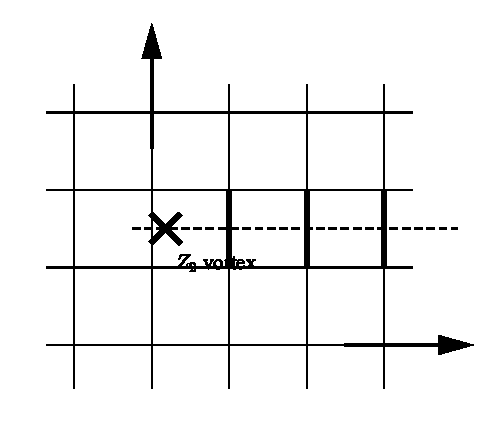
\includegraphics[width=0.72\textwidth]{fig_9.4.pdf}
\caption*{图 9.4\quad 沿粗线所示的链接翻转 $U_{ij}$ 的符号，就产生一个 $Z_2$ 涡旋。这里 $\Theta_{ij}=1$，唯有粗线所示的链接上 $\Theta_{ij}=-1$。}
\end{figure}

\subsection{$Z_2$ 自旋液体中的 $Z_2$ 涡旋}

\begin{keypoints}
\item $Z_2$ 自旋液体态含有一种 $Z_2$ 涡旋激发，它既不携带自旋也不携带电荷。
\item 把一个 $Z_2$ 涡旋绑定到自旋子上，会使自旋子的统计性从玻色性变为费米性，或从费米性变为玻色性。
\end{keypoints}

除自旋子外，$Z_2$ 自旋液体态中还有另一类准粒子激发（Wen, 1991a）。这种激发在平均场理论中以拓扑孤子（topological soliton）的形式出现，对应于 $Z_2$ 规范场的 $\pi$ 通量，因此我们将把这种新激发称为 $Z_2$ 涡旋。它通过沿一串链接翻转 $u_{ij}$ 的符号产生（见图 9.4），由下列拟设描写：
\begin{equation*}
\tilde{u}_{ij}=\bar{u}_{ij}\Theta_{ij}
\tag{9.2.38}
\end{equation*}
其中 $\Theta_{ij}$ 已在图 9.4 中说明。$Z_2$ 涡旋位于弦的端点。注意，在远离 $Z_2$ 涡旋处，$\tilde{u}_{ij}$ 局域地规范等价于 $\bar{u}_{ij}$，因此符号翻转的 $u_{ij}$ 弦不耗费任何能量，也观测不到。拟设 $\tilde{u}_{ij}$ 实际上描写的是位于弦端点的一个局域激发。

由于 $u_{ij}$ 决定自旋子的跳跃幅，当自旋子绕 $Z_2$ 涡旋跳行一周时会多出一个负号。因此，对自旋子而言 $Z_2$ 涡旋表现得像一个 $\pi$ 通量。根据 7.1.2 节的讨论，我们发现把一个 $Z_2$ 涡旋绑定到一个自旋子上，会把自旋子的统计性从费米性变为玻色性。因此，$Z_2$ 自旋液体既含有玻色统计的中性自旋-1/2 激发，也含有费米统计的中性自旋-1/2 激发。

\subsection*{问题 9.2.5}

证明：对于式 (9.2.38) 的 $Z_2$ 涡旋拟设，通过回路 $C$ 的 $SU(2)$ 通量与基态拟设 $u_{ij}$ 通过同一回路的 $SU(2)$ 通量相同，除非回路 $C$ 包围着涡旋。由于平均场能量是 $SU(2)$ 通量的函数，上述结果表明符号翻转的 $u_{ij}$ 弦不耗费能量。

\subsection{稳定的无能隙 $Z_2$ 自旋液体}

\begin{keypoints}
\item 存在许多不同的稳定自旋液体态——$Z_2$ 自旋液体态。其中一些可以具有无能隙的自旋子激发。
\item 这些态具有完全相同的对称性。没有办法利用对称性来刻画这些不同的自旋液体态。
\end{keypoints}

除了式 (9.2.35) 之外，对于 $Z_2$ 对称自旋液体我们还可以写下另一个拟设（Wen, 2002c）：
\begin{equation*}
u_{\pmb{i},\pmb{i}+\pmb{x}}=\mathrm{i}\eta\tau^{0}-\chi(\tau^{3}-\tau^{1}),\qquad u_{\pmb{i},\pmb{i}+\pmb{y}}=\mathrm{i}\eta\tau^{0}-\chi(\tau^{3}+\tau^{1}),\qquad a_0^{l}=0,
\tag{9.2.39}
\end{equation*}
其中 $\chi$ 与 $\eta$ 均不为零。当 $\chi=0$ 时，上述拟设成为 $SU(2)$ 无能隙自旋液体；当 $\eta=0$ 时，成为 $SU(2)$ 线性自旋液体。为了证明式 (9.2.39) 的拟设描写一个对称自旋液体，我们必须证明它在下列对称变换与规范变换的组合 $G_xT_x$、$G_yT_y$、$G_{P_x}P_x$、$G_{P_y}P_y$、$G_{P_{xy}}P_{xy}$ 与 $G_TT$ 下不变。我们发现，如果选取规范变换为
\begin{equation*}
\begin{array}{lll}
G_x=\tau^{0}, & \quad G_y=\tau^{0}, & \quad G_T=(-)^{i}\tau^{0},\\[2pt]
G_{P_x}=\mathrm{i}(-)^{i_x}\dfrac{\tau^{1}+\tau^{3}}{\sqrt{2}}, & \quad G_{P_y}=\mathrm{i}(-)^{i_y}\dfrac{\tau^{1}-\tau^{3}}{\sqrt{2}}, & \quad G_{P_{xy}}=\mathrm{i}\tau^{3},
\end{array}
\tag{9.2.40}
\end{equation*}
则对称变换再接着相应的规范变换，将保持拟设不变。

利用时间反演对称性，我们可以证明拟设 (9.2.39) 中取零值的 $a_0^{l}$ 确实满足约束 (9.2.29)。这是因为在组合时间反演变换 $G_TT$ 下 $a_0^{l}\to-a_0^{l}$。由于 $a_0^{l}=0$ 的拟设在 $G_TT$ 下不变，非零 $a_0^{l}$ 的平均场基态能量满足 $E_{\mathrm{ground}}(a_0^{l})=E_{\mathrm{ground}}(-a_0^{l})$，于是当 $a_0^{l}=0$ 时 $\partial E_{\mathrm{ground}}/\partial a_0^{l}=0$。事实上，任何只在两个不交叠子格之间有链接的拟设（即非阻挫拟设），只要 $a_0^{l}=0$，就是时间反演对称的。对这类拟设（包括拟设 (9.2.39)），取零值的 $a_0^{l}$ 满足约束 (9.2.29)。

自旋子谱由下式给出（见图 9.10(a)）
\begin{equation*}
E_{\pm}=2\eta(\sin(k_x)+\sin(k_y))\pm 2|\chi|\sqrt{2\cos^{2}(k_x)+2\cos^{2}(k_y)}
\end{equation*}
自旋子有两个费米点和两个小的费米口袋（Fermi pocket）（当 $\eta$ 小时）。$SU(2)$ 通量是非平凡的。而且，$SU(2)$ 通量 $P_{C_1}$ 与 $P_{C_2}$ 互不对易，其中 $C_1=\pmb{i}\to\pmb{i}+\pmb{x}\to\pmb{i}+\pmb{x}+\pmb{y}\to\pmb{i}+\pmb{y}\to\pmb{i}$ 与 $C_2=\pmb{i}\to\pmb{i}+\pmb{y}\to\pmb{i}-\pmb{x}+\pmb{y}\to\pmb{i}-\pmb{x}\to\pmb{i}$ 是两个具有同一基点的回路。非共线 $SU(2)$ 通量把 $SU(2)$ 规范结构破缺到 $Z_2$ 规范结构。我们将把式 (9.2.39) 描写的自旋液体称为 $Z_2$ 无能隙自旋液体。\footnote{$Z_2$ 无能隙自旋液体是 9.4.3 节中分类的 $Z_2$ 自旋液体之一，其投影对称群标记为 Z2Ax12(12)n（见 9.4.3 节及式 (9.4.16)）。}其低能有效理论由无质量狄拉克费米子和具有小费米面的费米子耦合到 $Z_2$ 规范场所描写。由于没有无能隙规范玻色子，规范涨落只能在自旋子之间传递短程相互作用。短程相互作用在低能下是不相关的，自旋子在低能下是自由费米子。因此，平均场 $Z_2$ 无能隙态是一个稳定态。这个稳定的平均场态暗示存在第二种真实的物理自旋液体（除 9.2.4 节讨论的 $Z_2$ 有能隙自旋液体之外）。这种自旋液体的物理性质可以由平均场理论得到。我们发现，$Z_2$ 无能隙自旋液体中的激发由中性的自旋-1/2 费米型准粒子描写！

第三种 $Z_2$ 对称自旋液体可以由下列阻挫拟设得到（Balents et al., 1998; Senthil and Fisher, 2000）：
\begin{align*}
a_0^{3}\neq 0,\qquad & a_0^{1,2}=0,\\
u_{\pmb{i},\pmb{i}+\pmb{x}}=\chi\tau^{3}+\eta\tau^{1},\qquad & u_{\pmb{i},\pmb{i}+\pmb{y}}=\chi\tau^{3}-\eta\tau^{1},\\
u_{\pmb{i},\pmb{i}+\pmb{x}+\pmb{y}}=+\gamma\tau^{3},\qquad & u_{\pmb{i},\pmb{i}-\pmb{x}+\pmb{y}}=+\gamma\tau^{3}.
\tag{9.2.41}
\end{align*}
该拟设具有平移、转动、宇称与时间反演对称性。它在组合变换 $G_{x,y}T_{x,y}$、$G_{P_x,P_y,P_{xy}}P_{x,y,xy}$ 与 $G_TT$ 下不变，其中
\begin{equation*}
\begin{array}{ccc}
G_x=\tau^{0}, & \quad G_y=\tau^{0}, & \quad G_T=\mathrm{i}\tau^{2},\\
G_{P_x}=\tau^{0}, & \quad G_{P_y}=\tau^{0}, & \quad G_{P_{xy}}=\mathrm{i}\tau^{3}.
\end{array}
\tag{9.2.42}
\end{equation*}
当 $a_0^{3}\neq 0$、$\chi\neq\pm\eta$ 且 $\chi\eta\neq 0$ 时，我们发现 $a_0^{l}\tau^{l}$ 与 $SU(2)$ 通量算符——例如穿过一个方格的 $SU(2)$ 通量 $P(C_{\mathrm{square}})$——不对易。\footnote{这里 $\tau^{l}a_0^{l}(\pmb{i})$ 可以看作通过一个零尺寸回路的 $SU(2)$ 通量。}因此，该拟设把 $SU(2)$ 规范结构破缺到 $Z_2$ 规范结构。自旋子谱由下式给出（见图 9.8(a)）
\begin{align*}
E_{\pm}&=\pm\sqrt{\epsilon^{2}(\pmb{k})+\Delta^{2}(\pmb{k})}\\
\epsilon(\pmb{k})&=2\chi(\cos(k_x)+\cos(k_y))+2\gamma(\cos(k_x+k_y)+\cos(k_x-k_y))+a_0^{3}\\
\Delta(\pmb{k})&=2\eta(\cos(k_x)-\cos(k_y))+a_0^{3}
\end{align*}
它只在该四个 $\pmb{k}$ 点无能隙，且具有线性色散。因此，式 (9.2.41) 描写的自旋液体是一个 $Z_2$ 线性自旋液体。\footnote{$Z_2$ 线性自旋液体由投影对称群 Z2A0032 或等价的 Z2A0013 描写（见 9.4.3 节）。}

$Z_2$ 有能隙拟设 (9.2.35)、$Z_2$ 无能隙拟设 (9.2.39) 与 $Z_2$ 线性拟设 (9.2.41) 在投影后给出三个自旋液体态。这三个态具有完全相同的对称性，所以我们不能用对称性来区分它们。为了找到一组新的量子数来刻画这三种不同的自旋液体，我们注意到：虽然三种 $Z_2$ 自旋液体具有相同的对称性，但它们的拟设分别在同样的对称平移之后跟着\emph{不同的}规范变换下不变（见式 (9.2.37)、(9.2.40) 与 (9.2.42)）。因此，三种自旋液体的平均场拟设的不变群各不相同，我们可以用这样的不变群来刻画不同的自旋液体。更详细和系统的讨论将在 9.4 节给出。

\subsection*{问题 9.2.6}

证明：如果规范变换由式 (9.2.40) 给出，则式 (9.2.39) 中的拟设在组合变换 $G_xT_x$、$G_yT_y$、$G_{P_x}P_x$、$G_{P_y}P_y$、$G_{P_{xy}}P_{xy}$ 与 $G_TT$ 下不变。

\subsection*{问题 9.2.7}

证明手征自旋态具有平移对称性和 $90^{\circ}$ 转动对称性。证明手征自旋态还具有组合对称性 $TP_x$、$TP_y$ 与 $TP_{xy}$。

\subsection{评注：平均场理论中的时间反演变换}

在时间反演变换（或自旋反转变换）下，$\pmb{S}_i\to-\pmb{S}_i$。由于本章只考虑自旋旋转不变的态，为方便起见，我们把 $T$ 变换定义为时间反演变换与自旋旋转变换的组合：$(S^{x},S^{y},S^{z})\to(S^{x},-S^{y},S^{z})$。我们将不严格地把它称为时间反演变换。

这样的变换可以由
\begin{equation*}
\psi\to\psi'=-\mathrm{i}\tau^{2}\psi^{*}
\tag{9.2.43}
\end{equation*}
生成。让我们用一个算符 $\mathcal{T}$ 来表示上述变换，即 $\mathcal{T}\psi\mathcal{T}^{-1}=-\mathrm{i}\tau^{2}\psi^{*}$。注意 $\mathcal{T}$ 把 $\mathrm{i}$ 变成 $-\mathrm{i}$，即 $\mathcal{T}^{-1}\mathrm{i}\mathcal{T}=-\mathrm{i}$。用 $f$ 费米子 (9.2.6) 表示，式 (9.2.43) 变为
\begin{equation*}
f\to\mathcal{T}f\mathcal{T}^{-1}=-\mathrm{i}\tau^{2}f^{*}
\end{equation*}
由 $\pmb{S}=\frac{1}{2}f^{\dagger}\pmb{\sigma}f$，我们发现 $\mathcal{T}$ 把 $\pmb{S}$ 变为
\begin{equation*}
\mathcal{T}\pmb{S}\mathcal{T}^{-1}=-\frac{1}{2}f^{\top}\pmb{\sigma}f^{*}=\frac{1}{2}f^{\dagger}\pmb{\sigma}^{\top}f=(S^{x},-S^{y},S^{z})
\end{equation*}
在平均场理论中，式 (9.2.43) 诱导平均场拟设的下列变换：
\begin{equation*}
\begin{aligned}
U_{ij}&\to U'_{ij}=(-\mathrm{i}\tau^{2})U_{ij}^{*}(\mathrm{i}\tau^{2})=-U_{ij}\\
a_0^{l}(\pmb{i})\tau^{l}&\to a_0^{\prime l}(\pmb{i})\tau^{l}=(-\mathrm{i}\tau^{2})(a_0^{l}(\pmb{i})\tau^{l})^{\top}(\mathrm{i}\tau^{2})=-a_0^{l}(\pmb{i})\tau^{l}
\end{aligned}
\tag{9.2.44}
\end{equation*}

% ------------------------------------------------------------
% 新增术语（ch9_c，书页 380–392，供术语表收录）：
%   loop variable 圈变量
%   SU(2)-flux operator SU(2) 通量算符
%   base point 基点
%   trivial / collinear / non-collinear SU(2) flux 平凡 / 共线 / 非共线 SU(2) 通量
%   mass term 质量项（ch3_e 已收）
%   uniform RVB state 均匀 RVB 态
%   staggered-flux state 交错通量态
%   d-wave pairing state d 波配对态
%   symmetric spin-liquid state 对称自旋液体态
%   Z₂-symmetric spin-liquid state Z₂ 对称自旋液体态
%   Z₂-gapped spin liquid Z₂ 有能隙自旋液体
%   Z₂-gapless spin liquid Z₂ 无能隙自旋液体
%   Z₂-linear spin liquid Z₂ 线性自旋液体（SU(2)/U(1)-linear state 同式：线性态）
%   sRVB (short-ranged resonating valence bond) state 短程共振价键（sRVB）态
%   Fermi pocket 费米口袋
%   topological soliton 拓扑孤子
%   unfrustrated / frustrated ansatz 非阻挫 / 阻挫拟设
%   invariant group 不变群
%   level (of Chern–Simons theory) level（Chern–Simons 理论的 level，不译）
%   spin–rotation transformation 自旋旋转变换
%   spin-reversal transformation 自旋反转变换
% ------------------------------------------------------------

% 块边界判定：
%   起点——书页 393（p408）顶部为图 9.5（属 9.2.7 节 T 变换讨论，前块止于书页 392 末的
%     式 (9.2.44)），页面首段 "The above describes ..." 为完整新句，无前块溢出内容，
%     故本块不设 %JOIN%，亦无需 %--C-TAIL-- 区。
%   终点——书页 405（p420）末句 "The key to obtaining the most general Z2A0013 ansatz
%     is to" 延续至书页 406（p421）首行 "find out which $u_m^\mu$ must vanish ..."。
%     按约定，半句译文（"……的关键是"）留在本文件正文最后，不写入任何 TAIL 区，
%     由 ch9_e 在其正文开头以 %JOIN% 续接。
% 蓝本问题记录：式 (9.4.11) 蓝本漏排 $G_y(\pmb{i})=\tau^0$ 一栏且上标误作 i_y（以图为准）；
%   式 (9.4.13) 蓝本作 $(-)^{m_y i_x}$，图上为 $(-)^{m i_x}$；书页 402 "±G_yT_x" 为
%   "±G_yT_y" 之误（据脚注 70 与式 (9.4.6)），已按本意译出并加译注。

\begin{figure}[H]
\centering
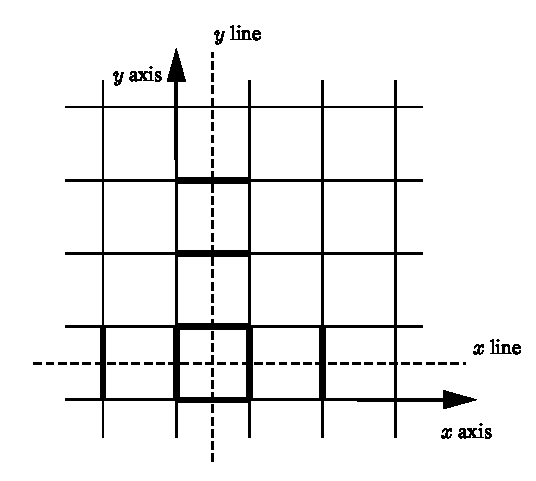
\includegraphics[width=0.72\textwidth]{fig_9.5.pdf}
\caption*{图 9.5\quad 跨越 $x$ 线与 $y$ 线的链获得一个额外的负号。}
\end{figure}

上述结果描述了平均场拟设在 $T$ 变换下的变换方式。自旋哈密顿量 (9.1.1) 与平均场哈密顿量 (9.2.4) 在时间反演变换下都是不变的。

\subsection*{问题 9.2.8}

试求在真实的时间反演变换 $S\to-S$ 下，$U_{ij}$ 与 $a_0^l(\pmb{i})$ 如何变换。

\section{有能隙自旋液体态中的拓扑序}

\begin{keypoints}
\item 自旋液体基态的拓扑简并。
\item 稳健的拓扑简并基态的存在意味着拓扑序的存在。
\end{keypoints}

我们用平均场理论构造了 $Z_2$ 有能隙态与手征自旋态。这两个自旋液体态的所有激发都有有限的能隙，并且保持平移对称性。我们想指出，这里研究的手征自旋液体与 $Z_2$ 有能隙自旋液体包含一些新型的序，它们既不能用对称性、也不能用与破缺对称性相联系的序参量来刻画。对 $Z_2$ 有能隙态而言，这一点相当明显，因为它不破缺任何对称性。手征自旋液体自发破缺了时间反演对称性与宇称对称性，并有相应的局域序参量来描述这种对称性破缺。正如我们后面将看到的，手征自旋液体还包含一些无法用对称性破缺描述的额外结构。由于手征自旋液体与 $Z_2$ 有能隙自旋液体都有有限的能隙，这类新型的序就是拓扑序。

正如 8.2.1 节所指出的，证明 $Z_2$ 有能隙态与手征自旋态具有非平庸拓扑序的一种办法，是证明这两个态具有拓扑简并的基态。让我们先考虑 $Z_2$ 有能隙态及其基态简并度。

我们把 $Z_2$ 有能隙态放到一个环面上，$x$ 与 $y$ 两个方向的格点数都取偶数。考虑由一个平均场解 $\bar{u}_{\pmb{ij}}$ 构造出的下列四个拟设：
\begin{equation*}
u_{\pmb{ij}}^{(m,n)}=(-)^{m s_x(\pmb{ij})}(-)^{n s_y(\pmb{ij})}\bar{u}_{\pmb{ij}}
\tag{9.3.1}
\end{equation*}
其中 $m,n=0,1$。这里 $s_{x,y}(\pmb{ij})$ 取 0 或 1：若链 $\pmb{ij}$ 跨越 $x$ 线，则 $s_x(\pmb{ij})=1$（见图 9.5），否则 $s_x(\pmb{ij})=0$；类似地，若链 $\pmb{ij}$ 跨越 $y$ 线，则 $s_y(\pmb{ij})=1$，否则 $s_y(\pmb{ij})=0$。

我们注意到，不同 $m$、$n$ 的 $u_{\pmb{ij}}^{(m,n)}$ 是局域规范等价的。这是因为，在无限系统上，改变 $u_{\pmb{ij}}\to(-)^{m s_x(\pmb{ij})}(-)^{n s_y(\pmb{ij})}u_{\pmb{ij}}$ 可以由一个 $SU(2)$ 规范变换 $u_{\pmb{ij}}\to W_{\pmb{i}}u_{\pmb{ij}}W_{\pmb{j}}^{\dagger}$ 生成，其中 $W_{\pmb{i}}=(-)^{m\Theta(i_x)}(-)^{n\Theta(i_y)}$，而 $\Theta(n)=1$ 若 $n>0$，$\Theta(n)=0$ 若 $n\leqslant0$。结果，不同的拟设 $u_{\pmb{ij}}^{(m,n)}$ 穿过每个方格的 $SU(2)$ 通量都相同。

对大系统而言，能量是 $u_{\pmb{ij}}$ 的局域函数，并且若 $u_{\pmb{ij}}$ 与 $\tilde{u}_{\pmb{ij}}$ 规范等价，则有 $F(u_{\pmb{ij}})=F(\tilde{u}_{\pmb{ij}})$。因此，不同 $u_{\pmb{ij}}^{(m,n)}$ 的能量相同（在热力学极限下）。另一方面，不同 $m$、$n$ 的 $u_{\pmb{ij}}^{(m,n)}$ 在整体意义上并不规范等价。一个自旋子沿 $x$（或 $y$）方向绕环面一整圈，会获得相位 $\mathrm{e}^{\mathrm{i}m\pi}$（或 $\mathrm{e}^{\mathrm{i}n\pi}$）。因此，$u_{\pmb{ij}}^{(mn)}\big|_{m,n=0,1}$ 描述不同的、相互正交的简并基态（另见问题 9.3.1）。这样我们就发现，$Z_2$ 有能隙态在环面上有四个简并基态（Read and Chakraborty, 1989; Wen, 1991a）。从自旋子绕环面一圈所获得的相位可以看出，$m$ 与 $n$ 标记穿过环面两个孔的 $\pi$ 通量的数目（见图 9.6）。四个简并基态对应于把 $\pi$ 通量穿入两个孔的不同方式。这一图像可以推广到更高亏格的黎曼面。简并基态可以这样构造：让 $\pi$ 通量以零个或一个单位穿过亏格为 $g$ 的黎曼面上的 $2g$ 个孔（见图 9.6）。这给出亏格为 $g$ 的黎曼面上 $2^{2g}$ 个简并基态。这种在不同黎曼面上的简并图案是 $Z_2$ 规范理论的标志。这些简并度与 $Z_2$ 涡旋激发的存在，以一种物理的方式表明，$Z_2$ 有能隙态的低能有效理论确实是一个 $Z_2$ 规范理论（见问题 9.3.1）。把自旋子包括进来之后，$Z_2$ 有能隙态的一阶平均场理论描述的是耦合到 $Z_2$ 规范理论上的费米子。$Z_2$ 有能隙态的物理性质可以从这样一个有效理论得到。

\begin{figure}[H]
\centering
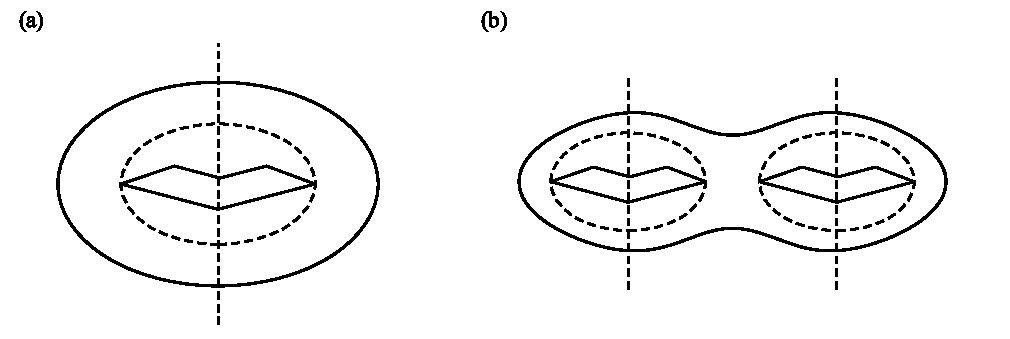
\includegraphics[width=0.72\textwidth]{fig_9.6.pdf}
\caption*{图 9.6\quad (a) 亏格 $g=1$ 的黎曼面（环面）上有 $2g=2$ 个孔；(b) 亏格 $g=2$ 的黎曼面上有 $2g=4$ 个孔。我们可以往这些孔里穿入零通量或 $\pi$ 通量。这给出 $Z_2$ 有能隙自旋液体的 $2^{2g}=4$ 或 16 个简并基态。}
\end{figure}

在一个有限的紧致化格点上，系统从一个基态隧穿到另一个基态的唯一途径是如下隧穿过程：先产生一对 $Z_2$ 涡旋，其中一个 $Z_2$ 涡旋绕环面一整圈，然后与另一个 $Z_2$ 涡旋湮没。这样的过程实质上给环面的孔添加了一个单位的 $\pi$ 通量，并使 $m$ 或 $n$ 改变 1。由于通量守恒，不同的基态无法通过任何局域涨落相互隧穿。这一结果的直接推论是，有限格点上不同基态之间的能量劈裂预期为 $\mathrm{e}^{-L/\xi}$ 的量级，其中 $1/\xi$ 与 $Z_2$ 涡旋的有限能隙相关。

在平均场理论中，基态的简并是规范不变性的一个后果。即使我们在原来的自旋哈密顿量中加入下列任意微扰，规范不变性仍然严格成立：
\begin{equation*}
\delta H=\sum\delta J_{ij}\,\pmb{S}_i\cdot\pmb{S}_j+\cdots
\tag{9.3.2}
\end{equation*}
其中 $\delta H$ 可以破坏平移对称性、旋转对称性等。因此上述论证依然成立，即使对修改后的哈密顿量，平均场基态仍保持四重简并。我们预期这一结果在平均场理论之外也成立。只要微扰足够弱、不至于关闭 $Z_2$ 涡旋的能隙，任何微扰都无法改变 $Z_2$ 有能隙态的基态简并度。因此，基态简并度是刻画自旋液体态不同相的一个普适量子数。这也表明 $Z_2$ 有能隙态中存在非平庸的拓扑序。

现在让我们考虑手征自旋态中的拓扑序。同样，我们想计算手征自旋态在比如环面上的基态简并度。计算基态简并度最容易的办法，是使用有效 Chern--Simons 理论 (9.1.28)，它描述 $a_{\mu}$ 集体模式的动力学。$U(1)$ Chern--Simons 理论的基态简并度已在 FQH 态的情形中讨论过。重复 8.2.1 节的计算，我们发现基态简并度是 2。我们想指出，这一二重简并是针对破缺 $T$ 与 $P$ 的基态的某一个扇区（sector）而言的，例如 $\langle\pmb{S}_1\cdot(\pmb{S}_2\times\pmb{S}_3)\rangle>0$ 的扇区。另一个扇区 $\langle\pmb{S}_1\cdot(\pmb{S}_2\times\pmb{S}_3)\rangle<0$ 也有两个简并基态。因此，总的基态简并度是 $4=2\times2$：一个因子 2 来自 $T$、$P$ 破缺，另一个因子 2 来自规范涨落。

由规范涨落引起的二重基态简并，源于手征自旋态中的非平庸拓扑序。这一简并依赖于空间的拓扑。在亏格为 $g$ 的黎曼面上，规范涨落给出 $2^g$ 个简并基态。这一简并度同样直接与规范结构相关，并且可以证明它对自旋哈密顿量的任意局域微扰都是稳健的。正如 FQH 态一样，手征自旋态的基态简并度与自旋子的分数统计密切相关。一般地可以证明，若自旋子具有分数统计 $\theta=\frac{p\pi}{q}$，则手征自旋态在亏格为 $g$ 的黎曼面上将有 $q^g$ 重简并的基态（Wen, 1990）。此外，作为非平庸拓扑序的另一个结果，手征自旋态具有无能隙的手征边缘激发（Wen, 1992）。

为了看出拓扑序概念的用处，让我们考虑下列物理问题：手征自旋态与 $Z_2$ 有能隙态之间的差别是什么？有人可能马上会说，这两个态有不同的对称性。然而，如果我们修改哈密顿量使 $T$ 与 $P$ 对称性破缺，两个态就会有相同的对称性。这时我们仍然可以问这两个态是否相同——即一个态能否不经相变而连续变形为另一个态。当 $T$ 与 $P$ 对称性被显式破缺时，手征自旋态有两个简并基态，而 $Z_2$ 有能隙态在环面上仍有四个简并基态。因此，即使具有相同的对称性，手征自旋态与 $Z_2$ 有能隙态也是不同的。两态的差别在于它们有不同的基态简并度和不同的拓扑序。

\subsection*{问题 9.3.1}

\textbf{非共线 $SU(2)$ 通量态中的 $Z_2$ 规范结构}

设 $u_{\pmb{ij}}=s_{ij}\bar{u}_{\pmb{ij}}$，其中 $s_{ij}=\pm1$，$\bar{u}_{\pmb{ij}}$ 是一个具有非共线 $SU(2)$ 通量的拟设。令 $|\{s_{ij}\}\rangle$ 为 $|\Psi_{\text{mean}}^{(u_{\pmb{ij}})}\rangle$ 的投影（见式 (9.2.11)），即
\begin{equation*}
|\{s_{ij}\}\rangle=\langle0_{\psi}|\prod_n\psi_{1,\pmb{i}_n}\psi_{2,\pmb{i}_n}|\Psi_{\text{mean}}^{(u_{\pmb{ij}})}\rangle.
\end{equation*}
\begin{enumerate}[label=(\alph*)]
\item 证明：与 $Z_2$ 规范理论中的态一样，若 $s_{ij}$ 与 $\tilde{s}_{ij}$ 通过一个 $Z_2$ 规范变换相联系，则 $|\{s_{ij}\}\rangle=|\{\tilde{s}_{ij}\}\rangle$。
\item 证明：式 (9.3.1) 所定义的四个 $u_{\pmb{ij}}^{(m,n)}$（其中 $\bar{u}_{\pmb{ij}}$ 为具有非共线 $SU(2)$ 通量的一般拟设）彼此不 $SU(2)$ 等价。（提示：考虑通过三个具有同一基点的回路 $C_{1,2,3}$ 的 $SU(2)$ 通量 $P(C_1)$、$P(C_2)$ 与 $P(C_3)$。这里 $C_1$ 与 $C_2$ 是两个小回路，满足 $[P(C_1),P(C_2)]\neq0$；$C_3$ 是绕环面一圈的大回路。）
\end{enumerate}

\section{对称自旋液体中的量子序}

\begin{keypoints}
\item 量子序是量子相中的非对称性破缺序。
\item 量子序既适用于有能隙量子态，也适用于无能隙量子态。
\end{keypoints}

在这一节中，我们将基于平均场拟设的不变群发展一种量子序理论。我们将把这个不变群称为投影对称群（projective symmetry group，PSG）。我们的理论使我们能够刻画并对数百种具有相同对称性的自旋液体态进行分类。与拓扑序的基态简并度不同，投影对称群既能刻画有能隙自旋液体，也能刻画无能隙自旋液体。

我们已经看到，可以有许多具有相同对称性的不同自旋液体。其中许多自旋液体占据相空间中的一个有限区域，代表稳定的量子相。于是我们在这里面临的处境与量子霍尔效应中的情形类似：存在许多无法用对称性和序参量区分的量子相。量子霍尔液体有有限的能隙，我们可以用基态简并度或更一般的拓扑序来描述这些不同态的内部序。这里我们仍然可以用拓扑序来描述有能隙自旋液体的内部序。然而，我们还有许多其他稳定的量子自旋液体，它们具有无能隙激发。

为了描述无能隙量子自旋液体（以及有能隙自旋液体）的内部序，我们在第 8 章中引入了一个新概念——量子序（quantum order）——它描述量子相中的非对称性破缺序（见图 8.7）。引入量子序的关键点是：量子相一般不能完全用破缺的对称性和局域序参量来刻画。量子霍尔态以及前几节构造的稳定自旋液体都说明了这一点。然而，要使量子序的概念有用，我们需要找到量子序的具体数学刻画。由于量子序既不由对称性也不由序参量描述，我们需要找到一种全新的刻画方式。Wen (2002c) 提出用投影对称群来刻画量子自旋液体中的量子（或拓扑）序。投影对称群的提出受到 9.2.6 节如下观察的启发：不同对称自旋液体的拟设，在同样的对称性变换之后跟上\emph{不同}的规范变换下不变。我们可以利用这些不同的规范变换来区分具有相同对称性的不同自旋液体。在接下来两节中，我们将在一般而形式化的框架下引入投影对称群。

\subsection{量子序与普适性质}

\begin{keypoints}
\item 定义一种新型的序，就是要找到一种新的普适性质。
\item （某一类）量子序可以用投影对称群描述。
\item 投影对称群是一个平均场拟设的不变群（或“对称性”群）。
\end{keypoints}

我们知道，定义一个量子相，就是要找出基态波函数的普适性质。我们可以利用普适性质把基态波函数归入若干普适类，使得每一类中的波函数具有相同的普适性质。这些普适类将对应于量子相。

然而，要找出多体波函数的普适性质是非常困难的。让我们考虑自由费米系统中的量子序（或普适类），以对这种困难获得一些直观认识。我们知道，自由费米子基态由一个 $N$ 个变量的反对称波函数描述。该反对称函数具有 Slater 行列式的形式，即 $\Psi(x_1,\ldots,x_N)=\det(M)$，其中 $M$ 的矩阵元由 $M_{mn}=\psi_n(x_m)$ 给出，而 $\psi_n$ 是单费米子波函数。寻找自由费米系统中量子序的第一步，是找到一种合理的方式把 Slater 行列式波函数归类。如果我们只知道实空间的多体函数 $\Psi(x_1,\ldots,x_N)$，这将是非常困难的。然而，如果我们用傅里叶变换把实空间波函数变到动量空间的波函数，就可以按照费米面拓扑把不同的波函数归类。要真正证明上述分类是合理的并对应于不同的量子相，我们需要证明：当基态波函数从一个类变到另一个类时，基态能量在转变点处总会出现奇异性。这就引出了我们对自由费米系统中量子序的理解（见 8.3.2 节）。费米面拓扑是一种普适性质，它使我们能够对不同的费米子波函数进行分类，并刻画自由费米子的不同量子相。这里我们想强调，如果没有傅里叶变换，就很难从实空间多体函数 $\Psi(x_1,\ldots,x_N)$ 中看出费米面拓扑。

为了理解自旋液体中的量子序，我们需要找到一种办法把自旋液体波函数 $\Psi_{\text{spin}}(\pmb{i}_1,\ldots,\pmb{i}_{N_t})$ 归类，其中 $\pmb{i}_m$ 标记自旋朝上的位置。这里缺少的是相应的“傅里叶”变换。正如费米面的拓扑一样，很难直接从实空间波函数中看出普适性质（如果有的话）。目前，我们还不知道如何对自旋液体波函数 $\Psi_{\text{spin}}$ 进行分类。

不过，我们不想就此放弃。受投影构造的启发，这里我们考虑一个较简单的问题来入手。我们把自己限制在可以由拟设 $(u_{\pmb{ij}},a_0^l\tau^l)$ 经式 (9.2.11) 得到的那一类多体波函数之内。我们不去寻找一般多体波函数的普适性质，而是设法找出这一子类中多体波函数的普适性质。由于这一子类中的多体波函数由拟设 $(u_{\pmb{ij}},a_0^l\tau^l)$ 标记，波函数的普适性质实际上就是拟设的普适性质，这大大简化了问题。诚然，有人可能会反驳说，拟设（或该子类波函数）的普适性质未必是自旋量子相的普适性质。对某些拟设来说情况确实如此。然而，如果拟设 $(u_{\pmb{ij}},a_0^l\tau^l)$ 所描述的平均场态对任何涨落都是稳定的（即在平均场态附近的任何涨落都不会引起红外发散），那么该平均场态就忠实地描述一个自旋量子态，拟设的普适性质也就是相应自旋量子相的普适性质。这样便在拟设的性质与物理自旋液体的性质之间建立起联系。

那么，拟设的普适性质应当是什么呢？受朗道对称性破缺序理论的启发，我们想在此提出：拟设的不变群（或“对称性”群）是拟设的一种普适性质。这个群将被称为投影对称群（PSG）。我们将在后面论证，某些 PSG 确实是量子相的普适性质，并且这些 PSG 可以用来刻画量子自旋液体中的量子序。

\subsection{投影对称群}

\begin{keypoints}
\item 投影对称群是对称性群的一个扩张。
\item 投影对称群对所有平均场相进行分类。
\item 只有当相应的平均场态稳定时，投影对称群才刻画物理自旋液体态中的量子序。
\end{keypoints}

让我们给出 PSG 的一个详细定义。PSG 是拟设的一种属性。它由保持拟设不变的所有变换构成。每个变换（即 PSG 中的每个元素）都可以写成一个对称性变换 $U$（如平移）与一个规范变换 $G_U$ 的组合。拟设在其 PSG 下的不变性可以表示为
\begin{align*}
G_U U(u_{\pmb{i}\pmb{j}}) &= u_{\pmb{i}\pmb{j}},\tag{9.4.1}\\
U(u_{\pmb{i}\pmb{j}}) &\equiv u_{U(\pmb{i}),U(\pmb{j})},\qquad G_U(u_{\pmb{i}\pmb{j}})\equiv G_U(\pmb{i})u_{\pmb{i}\pmb{j}}G_U^{\dagger}(\pmb{j}),\qquad G_U(\pmb{i})\in SU(2),
\end{align*}
对每个 $G_UU\in\text{PSG}$ 上式都成立。

每个 PSG 都包含一个特殊的子群，我们称之为不变规范群（invariant gauge group，IGG）。一个拟设的 IGG（记作 $\mathcal{G}$）由保持该拟设不变的所有纯规范变换构成：
\begin{equation*}
\mathcal{G}=\{W_{\pmb{i}}\,|\,W_{\pmb{i}}u_{\pmb{i}\pmb{j}}W_{\pmb{j}}^{\dagger}=u_{\pmb{i}\pmb{j}},\ W_{\pmb{i}}\in SU(2)\}
\tag{9.4.2}
\end{equation*}
如果我们想把 IGG 与一个对称性变换联系起来，那么相应的变换就是恒等对称性变换。

如果 IGG 是非平庸的，那么对一个固定的对称性变换 $U$，可以存在许多规范变换 $G_U$ 使得 $G_UU$ 保持拟设不变。若 $G_UU$ 在 $u_{\pmb{i}\pmb{j}}$ 的 PSG 中，则 $GG_UU$ 也在 PSG 中的充要条件是 $G\in\mathcal{G}$。这样，对每个对称性变换 $U$，$G_U$ 的不同选取与 IGG 中的元素一一对应。从上述定义我们看到，一个拟设的 PSG、IGG 与对称性群（symmetry group，SG）之间有如下关系：
\begin{equation*}
SG=PSG/IGG
\end{equation*}
这一关系告诉我们，PSG 是对称性群的一个投影表示，或称一个扩张（extension）。\footnote{更一般地，如果群 PSG 包含一个正规子群 IGG，使得 $PSG/IGG=SG$，我们就说群 PSG 是群 SG 的一个扩张。}

当然，两个规范等价拟设 $u_{\pmb{i}\pmb{j}}$ 与 $W(\pmb{i})u_{\pmb{i}\pmb{j}}W^{\dagger}(\pmb{j})$ 的 PSG 彼此相关。由 $WG_UU(u_{\pmb{i}\pmb{j}})=W(u_{\pmb{i}\pmb{j}})$，其中 $W(u_{\pmb{i}\pmb{j}})\equiv W(\pmb{i})u_{\pmb{i}\pmb{j}}W^{\dagger}(\pmb{j})$，我们发现
\begin{equation*}
WG_UUW^{-1}W(u_{\pmb{i}\pmb{j}})=WG_UW_U^{-1}UW(u_{\pmb{i}\pmb{j}})=W(u_{\pmb{i}\pmb{j}})
\end{equation*}
其中 $W_U\equiv UWU^{-1}$ 由 $W_U(\pmb{i})=W(U(\pmb{i}))$ 给出。这样，若 $G_UU$ 在拟设 $u_{\pmb{i}\pmb{j}}$ 的 PSG 中，则 $(WG_UW_U)U$ 在规范变换后的拟设 $W(\pmb{i})u_{\pmb{i}\pmb{j}}W^{\dagger}(\pmb{j})$ 的 PSG 中。我们看到，在规范变换 $W(\pmb{i})$ 之后，与对称性变换 $U$ 相联系的规范变换 $G_U$ 按如下方式改变：
\begin{equation*}
G_U(\pmb{i})\to W(\pmb{i})G_U(\pmb{i})W^{\dagger}(U(\pmb{i}))
\tag{9.4.3}
\end{equation*}

由于 PSG 是拟设的一种属性，我们可以把共享同一 PSG 的所有拟设归成一类。我们宣称，这样的类是一个普适类，对应于一个量子相。\footnote{更精确地说，这样的类由一个或若干个对应于量子相的普适类构成。（关于这一点的更详细讨论见 9.9 节。）}正是在这个意义上，我们说量子序由 PSG 刻画。

把量子序的 PSG 刻画与对称性破缺序的对称性刻画加以比较是很有启发的。我们知道，对称性破缺序可以由它的对称性性质描述。在数学上，我们说对称性破缺序由它的对称性群刻画。类似地，量子序也由群刻画。差别在于，量子序由 PSG——对称性群的扩张——刻画。我们看到，用投影对称群描述量子序，与用对称性群描述对称性破缺序，在概念上是相似的。我们还看到，具有相同对称性的量子态可以有许多不同的量子序，因为一个对称性群通常可以有许多不同的扩张。

除了能够刻画对称性破缺序之外，对称性破缺序的对称性描述还非常有用，因为它使我们无需了解系统的细节就能得到许多普适性质，例如无能隙 Nambu--Goldstone 模的数目。类似地，知道了一个量子序的 PSG，也使我们无需了解量子系统的细节就能得到它的低能性质。在 9.10 节中我们将证明，PSG 能够产生并保护低能规范涨落。事实上，低能规范涨落的规范群就是拟设的 IGG。这推广了 9.2.2 节得到的结果。除了无能隙规范玻色子之外，PSG 还能产生并保护无能隙费米子激发及其晶体动量。这些无能隙费米子甚至可以在纯玻色模型中产生。我们看到，无能隙规范玻色子与无能隙费米子可以有一个统一的起源——量子序。

这里我们想强调，PSG 真正分类的是不同的平均场相。连续的平均场相变总是伴随着 PSG 的改变。因此，严格说来，上述关于 PSG 及其物理含义的讨论只适用于平均场理论。然而，有些平均场态对涨落是稳定的。这些稳定平均场态的 PSG 就可以应用于相应的物理自旋液体，并描述这些自旋液体中真实的量子序。另一方面，也存在对涨落不稳定的平均场态。在这种情形下，相应的 PSG 可能不描述任何真实的量子序。

\subsection{对称 $Z_2$ 自旋液体的分类}

\begin{keypoints}
\item 我们分类了其 PSG 为格点对称性群（SG）之 $Z_2$ 扩张的所有平均场拟设，即 $PSG/Z_2=SG$。
\item 存在超过 100 种对称 $Z_2$ 自旋液体。
\item 不变 PSG 与代数 PSG 的概念。
\end{keypoints}

作为自旋液体量子序 PSG 理论的一个应用，我们想对与平移变换相联系的 PSG 进行分类。为简单起见，我们把 IGG $\mathcal{G}$ 限制为 $Z_2$。也就是说，我们想找出平移群的所有 $Z_2$ 扩张。

当 $\mathcal{G}=Z_2$ 时，它只含两个元素——规范变换 $G_1$ 与 $G_2$：
\begin{equation*}
\mathcal{G}=\{G_1,G_2\},\qquad G_1(\pmb{i})=\tau^0,\qquad G_2(\pmb{i})=-\tau^0.
\end{equation*}
一个拟设的 IGG 要为 $\mathcal{G}=Z_2$，该拟设就必须产生非共线的 $SU(2)$ 通量；否则 IGG 将大于 $Z_2$。拟设中的非共线 $SU(2)$ 通量把 $SU(2)$ 规范结构破缺到 $Z_2$ 规范结构，相应的自旋液体是一个 $Z_2$ 自旋液体。我们看到，平移群的 $Z_2$ 扩张在物理上对所有\emph{只}具有平移对称性的 $Z_2$ 自旋液体进行了分类。

考虑一个具有平移对称性的 $Z_2$ 自旋液体。作为平移群的 $Z_2$ 扩张，它的 PSG 由四个元素 $\pm G_xT_x$ 与 $\pm G_yT_y$ 生成\footnote{译注：原文作“$\pm G_yT_x$”，据式 (9.4.6) 及脚注（原书脚注 70）应为 $\pm G_yT_y$ 之误，此处按本意译出。}，其中
\begin{equation*}
T_x(u_{\pmb{ij}})=u_{\pmb{i}-\pmb{x},\,\pmb{j}-\pmb{x}},\qquad T_y(u_{\pmb{ij}})=u_{\pmb{i}-\pmb{y},\,\pmb{j}-\pmb{y}}.
\end{equation*}
由于拟设的平移对称性，我们可以选取一个规范，使拟设的所有 $SU(2)$ 通量算符都是平移不变的。也就是说，若两个回路 $C_1$ 与 $C_2$ 通过一个平移相联系，则 $P_{C_1}=P_{C_2}$。我们把这样的规范称为均匀规范（uniform gauge）。

在变换 $G_xT_x$ 下，以 $\pmb{i}$ 为基点的 $SU(2)$ 通量算符 $P_C$ 按如下方式变换：$P_C\to G_x(\pmb{i}')P_{T_x(C)}G_x^{\dagger}(\pmb{i}')\allowbreak=G_x(\pmb{i}')P_CG_x^{\dagger}(\pmb{i}')$，其中 $\pmb{i}'=T_x\pmb{i}$ 是平移后的回路 $T_x(C)$ 的基点。我们看到，$P_C$ 在均匀规范下的平移不变性要求：对任何回路 $C$ 都有 $G_x(\pmb{i}')P_CG_x^{\dagger}(\pmb{i}')=P_C$。同样，$G_y$ 也满足类似的条件。由于以同一基点为基点的不同 $SU(2)$ 通量算符互不对易，$G_{x,y}(\pmb{i})$ 在每个格点只能取 $\pm\tau^0$ 两个值之一。

我们注意到，形如 $W(\pmb{i})=\pm\tau^0$ 的依赖格点的规范变换不改变 $SU(2)$ 通量算符的平移不变性质。因此，我们可以利用这类规范变换，通过式 (9.4.3) 进一步简化 $G_{x,y}$。首先，我们可以选取规范使（见问题 9.4.1）
\begin{equation*}
G_y(\pmb{i})=\tau^0.
\tag{9.4.4}
\end{equation*}
我们注意到，满足 $W(\pmb{i})=W(i_x)$ 的规范变换不改变条件 $G_y(\pmb{i})=\tau^0$。我们可以利用这类规范变换使
\begin{equation*}
G_x(i_x,\ i_y=0)=\tau^0.
\tag{9.4.5}
\end{equation*}
由于 $x$ 与 $y$ 方向的平移相互对易，$G_{x,y}$ 必须满足（对任何拟设，无论是不是 $Z_2$）
\begin{equation*}
G_xT_xG_yT_y(G_xT_x)^{-1}(G_yT_y)^{-1}=G_xT_xG_yT_yT_x^{-1}G_x^{-1}T_y^{-1}G_y^{-1}\in\mathcal{G}.
\tag{9.4.6}
\end{equation*}
这意味着
\begin{equation*}
G_x(\pmb{i})G_y(\pmb{i}-\pmb{x})G_x^{-1}(\pmb{i}-\pmb{y})G_y(\pmb{i})^{-1}\in\mathcal{G}
\tag{9.4.7}
\end{equation*}
对 $Z_2$ 自旋液体，由于式 (9.4.4)，式 (9.4.7) 约化为
\begin{equation*}
G_x(\pmb{i})G_x^{-1}(\pmb{i}-\pmb{y})=+\tau^0
\tag{9.4.8}
\end{equation*}
或
\begin{equation*}
G_x(\pmb{i})G_x^{-1}(\pmb{i}-\pmb{y})=-\tau^0
\tag{9.4.9}
\end{equation*}
与式 (9.4.5) 和 (9.4.4) 联立，我们发现式 (9.4.8) 与 (9.4.9) 成为
\begin{equation*}
G_x(\pmb{i})=\tau^0,\qquad G_y(\pmb{i})=\tau^0
\tag{9.4.10}
\end{equation*}
以及
\begin{equation*}
G_x(\pmb{i})=(-)^{i_x}\tau^0,\qquad G_y(\pmb{i})=\tau^0
\tag{9.4.11}
\end{equation*}
这样，平移群只有两个规范不等价的 $Z_2$ 扩张。这两个 PSG 由 $G_xT_x$ 与 $G_yT_y$ 生成，其中的 $G_{x,y}$ 由式 (9.4.10) 与 (9.4.11) 给出。\footnote{我们想指出，若 $G_x$ 与 $G_y$ 由式 (9.4.8) 给出，则 $G_xT_x$ 与 $G_yT_y$ 满足通常的平移代数 $G_xT_xG_yT_y=G_yT_yG_xT_x$。当 $G_x$ 与 $G_y$ 由式 (9.4.9) 给出时，$G_xT_x$ 与 $G_yT_y$ 满足磁平移代数 $G_xT_xG_yT_y=-G_yT_yG_xT_x$。}在 PSG 分类下，\emph{只}具有平移对称性而没有其他对称性的 $Z_2$ 自旋液体只有两种类型。在 PSG (9.4.10) 下不变的拟设具有形式
\begin{equation*}
u_{\pmb{i},\pmb{i}+\pmb{m}}=u_{\pmb{m}}
\tag{9.4.12}
\end{equation*}
而在 PSG (9.4.11) 下不变的拟设具有形式
\begin{equation*}
u_{\pmb{i},\pmb{i}+\pmb{m}}=(-)^{m i_x}u_{\pmb{m}}
\tag{9.4.13}
\end{equation*}

通过上面的例子我们看到，PSG 是一个非常强有力的工具。对于具有给定对称性和低能规范结构的（平均场）自旋液体，它可以给出完全的分类。

在上文中，我们研究了只具有平移对称性而无其他对称性的 $Z_2$ 自旋液体，发现这样的自旋液体只有两种类型。然而，如果自旋液体具有更多对称性，类型就会多得多。Wen (2002c) 利用 PSG 得到了对称 $Z_2$ 自旋液体的分类。这一分类来自如下观察：规范变换 $G_{x,y}$、$G_{P_x,P_y,P_{xy}}$ 与 $G_T$ 必须满足某些与式 (9.4.7) 类似的代数关系。求解这些代数关系并剔除规范等价的解，我们发现，由平移、宇称与时间反演变换 $\{T_{x,y},P_{x,y,xy},T\}$ 生成的对称性群共有 272 个不同的 $Z_2$ 扩张。这里我们仅列出这 272 个 $Z_2$ PSG。这些 PSG 由 $(G_xT_x,\ G_yT_y,\ G_TT,\ G_{P_x}P_x,\ G_{P_y}P_y,\ G_{P_{xy}}P_{xy})$ 生成。PSG 可以分成两类。第一类为
\begin{equation*}
\begin{array}{rcl}
G_x(\pmb{i})=\tau^0, & & G_y(\pmb{i})=\tau^0\\[2pt]
G_{P_x}(\pmb{i})=\eta_{xpx}^{i_x}\eta_{xpy}^{i_y}g_{P_x}, & & G_{P_y}(\pmb{i})=\eta_{xpy}^{i_x}\eta_{xpx}^{i_y}g_{P_y}\\[2pt]
G_{P_{xy}}(\pmb{i})=g_{P_{xy}}, & & G_T(\pmb{i})=\eta_t^{\pmb{i}}g_T
\end{array}
\tag{9.4.14}
\end{equation*}
第二类为
\begin{equation*}
\begin{array}{rcl}
G_x(\pmb{i})=(-)^{i_x}\tau^0, & & G_y(\pmb{i})=\tau^0\\[2pt]
G_{P_x}(\pmb{i})=\eta_{xpx}^{i_x}\eta_{xpy}^{i_y}g_{P_x}, & & G_{P_y}(\pmb{i})=\eta_{xpy}^{i_x}\eta_{xpx}^{i_y}g_{P_y}\\[2pt]
G_{P_{xy}}(\pmb{i})=(-)^{i_x i_y}g_{P_{xy}}, & & G_T(\pmb{i})=\eta_t^{\pmb{i}}g_T
\end{array}
\tag{9.4.15}
\end{equation*}
这里三个 $\eta$ 可以各自独立地取 $\pm1$ 两个值。$g$ 有 17 种不同的选择，列于表 9.1 之中。因此，共有 $2\times17\times2^{3}=272$ 个不同的 PSG。它们可能给出二维正方格点上 272 种不同类型的对称 $Z_2$ 自旋液体。

为了标记这 272 个 PSG，我们提出如下方案：
\begin{equation*}
\text{Z2A}(g_{px})_{\eta_{xpx}}(g_{py})_{\eta_{xpy}}g_{pxy}(g_t)_{\eta_t},
\tag{9.4.16}
\end{equation*}
\begin{equation*}
\text{Z2B}(g_{px})_{\eta_{xpx}}(g_{py})_{\eta_{xpy}}g_{pxy}(g_t)_{\eta_t}.
\tag{9.4.17}
\end{equation*}
标记 Z2A… 对应式 (9.4.14) 的情形，标记 Z2B… 对应式 (9.4.15) 的情形。一个典型的标记形如 $\text{Z2A}\tau_{+}^{1}\tau_{-}^{2}\tau^{12}\tau_{-}^{3}$。我们还将使用一种缩写记号：把 $(\tau^{0},\tau^{1},\tau^{2},\tau^{3})$ 或 $(\tau_{+}^{0},\tau_{+}^{1},\tau_{+}^{2},\tau_{+}^{3})$ 换成 $(0,1,2,3)$，把 $(\tau_{-}^{0},\tau_{-}^{1},\tau_{-}^{2},\tau_{-}^{3})$ 换成 $(n,x,y,z)$。例如，$\text{Z2A}\tau_{+}^{1}\tau_{-}^{0}\tau^{12}\tau_{-}^{3}$ 可缩写为 Z2A1n(12)z。

严格说来，这 272 个不同的 $Z_2$ PSG 是所谓的代数 PSG（algebraic PSG）。代数 PSG 定义为对称性群的扩张。代数 PSG 不同于不变 PSG（invariant PSG），后者定义为保持一个拟设 $u_{\pmb{ij}}$ 不变的所有变换的集合。虽然不变 PSG 必定是代数 PSG，但代数 PSG 未必是不变 PSG。这是因为某些代数 PSG 具有如下性质：在代数 PSG $G_1$ 下不变的\emph{任何}拟设 $u_{\pmb{ij}}$，实际上可能在一个更大的 PSG $G_2$ 下也不变。这时，原来的 PSG $G_1$ 不可能是该拟设的不变 PSG，拟设的不变 PSG 实际上由更大的 PSG $G_2$ 给出。如果我们把自己限制在通过拟设 $u_{\pmb{ij}}$ 构造的自旋液体上，那么就应当舍弃那些不是不变 PSG 的代数 PSG，因为这些代数 PSG 并不刻画平均场自旋液体。

\begin{center}
\small 表 9.1\quad $Z_2$ PSG 的 $g_{P_{xy}}$、$g_{P_x}$、$g_{P_y}$ 与 $g_T$ 的 17 种选择。这里 $\tau^{ab}=(\tau^{a}+\tau^{b})/\sqrt{2}$，$\tau^{a\bar{b}}=(\tau^{a}-\tau^{b})/\sqrt{2}$。\\[6pt]
\begin{tabular}{cccccccc}
\toprule
$g_{P_{xy}}$ & $g_{P_x}$ & $g_{P_y}$ & $g_T$ & $g_{P_{xy}}$ & $g_{P_x}$ & $g_{P_y}$ & $g_T$ \\
\midrule
$\tau^0$ & $\tau^0$ & $\tau^0$ & $\tau^0$ & $\tau^0$ & $\mathrm{i}\tau^3$ & $\mathrm{i}\tau^3$ & $\tau^0$ \\
$\mathrm{i}\tau^3$ & $\tau^0$ & $\tau^0$ & $\tau^0$ & $\mathrm{i}\tau^3$ & $\mathrm{i}\tau^3$ & $\mathrm{i}\tau^3$ & $\tau^0$ \\
$\mathrm{i}\tau^3$ & $\mathrm{i}\tau^1$ & $\mathrm{i}\tau^1$ & $\tau^0$ & $\tau^0$ & $\tau^0$ & $\tau^0$ & $\mathrm{i}\tau^3$ \\
$\tau^0$ & $\mathrm{i}\tau^3$ & $\mathrm{i}\tau^3$ & $\mathrm{i}\tau^3$ & $\tau^0$ & $\mathrm{i}\tau^1$ & $\mathrm{i}\tau^1$ & $\mathrm{i}\tau^3$ \\
$\mathrm{i}\tau^3$ & $\tau^0$ & $\tau^0$ & $\mathrm{i}\tau^3$ & $\mathrm{i}\tau^3$ & $\mathrm{i}\tau^3$ & $\mathrm{i}\tau^3$ & $\mathrm{i}\tau^3$ \\
$\mathrm{i}\tau^3$ & $\mathrm{i}\tau^1$ & $\mathrm{i}\tau^1$ & $\mathrm{i}\tau^3$ & $\mathrm{i}\tau^1$ & $\tau^0$ & $\tau^0$ & $\mathrm{i}\tau^3$ \\
$\mathrm{i}\tau^1$ & $\mathrm{i}\tau^3$ & $\mathrm{i}\tau^3$ & $\mathrm{i}\tau^3$ & $\mathrm{i}\tau^1$ & $\mathrm{i}\tau^1$ & $\mathrm{i}\tau^1$ & $\mathrm{i}\tau^3$ \\
$\mathrm{i}\tau^1$ & $\mathrm{i}\tau^2$ & $\mathrm{i}\tau^2$ & $\mathrm{i}\tau^3$ & $\mathrm{i}\tau^{12}$ & $\mathrm{i}\tau^1$ & $\mathrm{i}\tau^2$ & $\mathrm{i}\tau^0$ \\
$\mathrm{i}\tau^{12}$ & $\mathrm{i}\tau^1$ & $\mathrm{i}\tau^2$ & $\mathrm{i}\tau^3$ & & & & \\
\bottomrule
\end{tabular}
\end{center}

我们发现，在 272 个代数 $Z_2$ PSG 中，至少有 76 个不是不变 PSG。因此，272 个代数 $Z_2$ PSG 至多能给出 196 种可能的 $Z_2$ 自旋液体。

\subsection{一个 $Z_2$ 与一个 $U(1)$ 投影对称群及其拟设}

\begin{keypoints}
\item 对给定的 PSG，我们可以找出其最普遍的拟设。这些拟设共有的物理性质，就是与该 PSG 相联系的普适性质。
\end{keypoints}

作为 $Z_2$ PSG 的一个应用，让我们构造在 Z2A0013 PSG 下不变的最普遍拟设：
\begin{equation*}
\begin{array}{rcl}
G_x(\pmb{i})=\tau^0, & & G_y(\pmb{i})=\tau^0\\[2pt]
G_{P_x}(\pmb{i})=\tau^0, & & G_{P_y}(\pmb{i})=\tau^0\\[2pt]
G_{P_{xy}}(\pmb{i})=\mathrm{i}\tau^1, & & G_T(\pmb{i})=\mathrm{i}\tau^3
\end{array}
\tag{9.4.18}
\end{equation*}
由 $G_xT_x$ 与 $G_yT_y$ 下的不变性，再考虑到 $G_x$ 与 $G_y$ 是平庸的，Z2A0013 拟设直接就是平移不变的，形式为 $u_{\pmb{i},\pmb{i}+\pmb{m}}=u_{\pmb{m}}^{\mu}\tau^{\mu}$。求出最普遍 Z2A0013 拟设的关键是

% ---- 块界备注：上句延续至书页 406（p421）首行 "find out which $u_m^\mu$ must vanish."
% ---- （"……找出哪些 $u_{\pmb{m}}^{\mu}$ 必须为零。"），请 ch9_e 以 %JOIN% 续接，勿重复勿遗漏。

% ---------------- 新增术语（ch9_d） ----------------
% | extension (of a group) | 扩张 |
% | projective representation | 投影表示 |
% | normal subgroup | 正规子群 |
% | invariant group | 不变群 |
% | symmetry group (SG) | 对称性群（SG） |
% | invariant PSG | 不变 PSG |
% | algebraic PSG | 代数 PSG |
% | uniform gauge | 均匀规范 |
% | magnetic translational algebra | 磁平移代数（ch7_a 已收“磁平移”） |
% | sector | 扇区 |
% | pure gauge transformation | 纯规范变换 |
% | collinearness | 共线性 |
% | thermodynamic limit | 热力学极限 |
% | flux conservation | 通量守恒 |
% | infra-red divergence | 红外发散 |
% | quantum phase | 量子相 |
% | universal property | 普适性质 |
% | topologically-degenerate ground state | 拓扑简并基态 |
% | first-order mean-field theory | 一阶平均场理论 |
% | Z2-gapped / Z2-gapless / Z2-linear spin liquid | Z2 有能隙 / 无能隙 / 线性自旋液体 |
% | SU(2)-gapless / SU(2)-linear state | SU(2) 无能隙态 / SU(2) 线性态 |
% | U(1)-linear state | U(1) 线性态 |
% | invariant gauge group (IGG) | 不变规范群（IGG）（术语表已收，本块首次正文出现） |
% | compactified lattice | 紧致化格点（compactification 紧致化已收） |

% 块边界判定：
%   起点——书页 406（p421）顶部为承接书页 405 的半句 "find out which $u_m^\mu$ must
%     vanish."（ch9_d 末句停在"……的关键是"），故本块正文首行以 %JOIN% 续接，
%     随后接本页其余正文。
%   终点——书页 418（p433）末段止于完整句 "The gapless spinons appear only at
%     $(\pi/2,\pm\pi/2)$."；书页 419（p434）顶部另起新段 "Knowing the translational
%     symmetry ..."（连同其后的式 (9.6.9)、9.6.2 节与问题 9.6.1–9.6.3），均属下一块。
%     本块自然结束，不设 TAIL 区。
% 蓝本问题记录（均已按图改正）：
%   1) 书页 406 蓝本作 $u_{ij}=\mathrm{i}u_{ij}^0\tau^0+w_{ij}^3\tau^3$，图上为
%      $u_{ij}^3\tau^3$（蓝本 OCR 之误）。
%   2) 式 (9.4.23)、(9.4.24) 蓝本行尾残留 "\tag {9}" 杂项，已删。
%   3) 式 (9.4.28) 蓝本把最后一个规范变换误作 $G_\Gamma$，图上为 $G_T$。
%   4) 9.4.5 节 U1A 标记行蓝本残损（"U1A$_{a_{\eta_x px}}$b$_{\eta_y px}$cd$_y$,"
%      与 "$G_{F_{xy}}$"、"If the corresponding G contains a $\tau^1$, and equal
%      to $\tau^0$ otherwise"），图上为 "U1A$a_{\eta_{xpx}}b_{\eta_{ypx}}cd_{\eta_t}$、
%      $G_{P_{xy}}$"，句子为 "They are equal to $\tau^1$ if the corresponding $G$
%      contains a $\tau^1$, and equal to $\tau^0$ otherwise."，已按图译出。
%   5) 式 (9.6.8) 第二行右列图上印作 $u_{\pmb{i},\pmb{i}+-\pmb{x}+2\pmb{y}}$（多印一
%      个加号），按本意译为 $u_{\pmb{i},\pmb{i}-\pmb{x}+2\pmb{y}}$。
%   6) 书页 418 的 $\Gamma$ 矩阵定义，蓝本排成两栏且重复 $\Gamma_4$；图上为两行
%      （$\Gamma_0,\Gamma_1,\Gamma_2$ / $\Gamma_3,\Gamma_4$），已按图重排。
%   7) 书页 411–412 "contruct"、"we would like to the study"、书页 406–407 跨页
%      "under under"、书页 415 "(9.2.34"（缺右括号）等为原书排印错误，按本意译出。

%JOIN%找出哪些 $u_{\pmb{m}}^{\mu}$ 必须为零。时间反演变换 $G_{T}T$ 与 $180^{\circ}$ 旋转 $G_{P_{x}}P_{x}G_{P_{y}}P_{y}$ 在这里起关键作用。$G_{T}T$ 下的不变性要求 $-u_{\pmb{m}}=\tau^{3}u_{\pmb{m}}\tau^{3}$，因此只有 $u_{\pmb{m}}^{1,2}$ 可以非零。$G_{P_{x}}P_{x}G_{P_{y}}P_{y}$ 下的不变性要求 $u_{\pmb{m}}=u_{-\pmb{m}}$，而由于 $u_{\pmb{m}}^{1,2}$ 为实数且 $u_{-\pmb{m}}=u_{\pmb{m}}^{\dagger}$，$u_{\pmb{m}}=u_{\pmb{m}}^{1}\tau^{1}+u_{\pmb{m}}^{2}\tau^{2}$ 总能满足这一要求，所以 $180^{\circ}$ 旋转不附加任何新条件。其余变换则把不同的 $u_{\pmb{m}}^{1,2}$ 联系起来。$G_{P_{xy}}P_{xy}$ 下的不变性要求 $u_{P_{xy}\pmb{m}}=\tau^{1}u_{\pmb{m}}\tau^{1}$，其中 $P_{xy}\pmb{m}=P_{xy}(m_{x},m_{y})=(m_{y},m_{x})$。于是，最普遍的 Z2A0013 拟设具有如下形式：
\begin{equation*}
\begin{array}{l}
u_{\pmb{m}}=u_{\pmb{m}}^{1}\tau^{1}+u_{\pmb{m}}^{2}\tau^{2}\\[2pt]
u_{P_{x}\pmb{m}}^{1,2}=u_{\pmb{m}}^{1,2},\qquad u_{P_{y}\pmb{m}}^{1,2}=u_{\pmb{m}}^{1,2}\\[2pt]
u_{P_{xy}\pmb{m}}^{1}=u_{\pmb{m}}^{1},\qquad u_{P_{xy}\pmb{m}}^{2}=-u_{\pmb{m}}^{2}
\end{array}
\end{equation*}
把式 (9.2.41) 中的 $(\tau^{3},\tau^{1})$ 换成 $(\tau^{1},\tau^{2})$，并把 $a_{0}$ 认同于 $u_{\pmb{m}=0}$，我们发现 $Z_{2}$ 线性自旋液体的拟设 (9.2.41) 是上述拟设的一个特例。因此，拟设 (9.2.41) 的 PSG 就是 Z2A0013 PSG，相应的自旋液体是一个 Z2A0013 自旋液体。

除了上面研究的 $Z_{2}$ 对称自旋液体之外，还可能存在低能规范群为 $U(1)$ 或 $SU(2)$ 的对称自旋液体。这类 $U(1)$ 对称或 $SU(2)$ 对称的自旋液体由 IGG 为 $U(1)$ 或 $SU(2)$ 的 PSG 分类。我们把这些 PSG 称为 $U(1)$ PSG 与 $SU(2)$ PSG。$U(1)$ PSG 与 $SU(2)$ PSG 已由 Wen (2002c) 算出，9.4.5 节将总结这些结果。

$U(1)$ PSG 中的一个由下式给出：
\begin{equation*}
\begin{array}{rcl}
G_{x}=g_{3}(\theta_{x})\mathrm{i}\tau^{1}, & & G_{y}=g_{3}(\theta_{y})\mathrm{i}\tau^{1},\\[2pt]
G_{P_{x}}=(-)^{i_{x}}g_{3}(\theta_{px}), & & G_{P_{y}}=(-)^{i_{y}}g_{3}(\theta_{py}),\\[2pt]
G_{P_{xy}}=g_{3}(\theta_{pxy})\mathrm{i}\tau^{1}, & & G_{T}=(-)^{\pmb{i}}g_{3}(\theta_{t}).
\end{array}
\tag{9.4.19}
\end{equation*}
其中
\begin{equation*}
g_{a}(\theta)\equiv\mathrm{e}^{\mathrm{i}\theta\tau^{a}}.
\end{equation*}
IGG 由 $\{g_{3}(\phi)\,|\,\phi\in[0,2\pi)\}$ 构成。这样的 PSG 标记为 U1Cn01n。在式 (9.4.27) 中取 $\eta_{xpx}=-1$、$\eta_{ypx}=+1$、$\eta_{pxy}=+1$ 与 $\eta_{t}=-1$ 即得到它。

让我们求出在 U1Cn01n PSG 下不变的最普遍拟设。要在 IGG 下不变，拟设必须对任意 $\theta$ 满足 $g_{3}(\theta)u_{\pmb{ij}}g_{3}^{\dagger}(\theta)=u_{\pmb{ij}}$，因此 $u_{\pmb{ij}}$ 必须具有 $u_{\pmb{ij}}=\mathrm{i}u_{\pmb{ij}}^{0}\tau^{0}+u_{\pmb{ij}}^{3}\tau^{3}$ 的形式。在平移变换 $G_{x}T_{x}$ 与 $G_{y}T_{y}$ 下的不变性要求 $u_{\pmb{ij}}^{0}$ 平移不变，而 $u_{\pmb{ij}}^{3}$ 在两个平移 $T_{x,y}$ 下变号。于是 $u_{\pmb{ij}}$ 具有形式 $u_{\pmb{i},\pmb{i}+\pmb{m}}=\mathrm{i}u_{\pmb{m}}^{0}\tau^{0}+(-)^{i}u_{\pmb{m}}^{3}\tau^{3}$。时间反演变换 $G_{T}T$ 下的不变性要求 $-u_{\pmb{m}}=(-)^{\pmb{m}}u_{\pmb{m}}$。我们发现，若 $\pmb{m}$ 为偶，则 $u_{\pmb{m}}^{0,3}=0$。\footnote{这里 $\pmb{m}$ 为偶（奇），若 $m_{x}+m_{y}$ 为偶（奇）。}$180^{\circ}$ 旋转 $G_{P_{x}}P_{x}G_{P_{y}}P_{y}$ 下的不变性要求 $u_{-\pmb{i},-\pmb{i}-\pmb{m}}=u_{-\pmb{i}-\pmb{m},-\pmb{i}}^{\dagger}=(-)^{\pmb{m}}u_{\pmb{i},\pmb{i}+\pmb{m}}$，这意味着 $-\mathrm{i}u_{\pmb{m}}^{0}\tau^{0}+(-)^{\pmb{i}+\pmb{m}}u_{\pmb{m}}^{3}\tau^{3}=(-)^{\pmb{m}}\big(\mathrm{i}u_{\pmb{m}}^{0}\tau^{0}+(-)^{\pmb{i}}u_{\pmb{m}}^{3}\tau^{3}\big)$。由此得到 $u_{\pmb{m}}^{0}=-(-)^{\pmb{m}}u_{\pmb{m}}^{0}$ 与 $u_{\pmb{m}}^{3}=u_{\pmb{m}}^{3}$，对 $u_{\pmb{m}}^{0,3}$ 没有给出新的约束。厄米关系 $u_{\pmb{i},\pmb{i}+\pmb{m}}^{\dagger}=u_{\pmb{i}+\pmb{m},\pmb{i}}$ 给出 $u_{\pmb{m}}^{0}=-u_{-\pmb{m}}^{0}$ 与 $u_{\pmb{m}}^{3}=(-)^{\pmb{m}}u_{-\pmb{m}}^{3}$。汇总上述条件，并计入 $G_{P_{x}}P_{x}$ 等的作用，我们发现最普遍的 U1Cn01n 拟设具有如下形式：
\begin{equation*}
\begin{array}{l}
u_{\pmb{i},\pmb{i}+\pmb{m}}=\mathrm{i}u_{\pmb{m}}^{0}\tau^{0}+(-)^{i}u_{\pmb{m}}^{3}\tau^{3}\\[2pt]
\qquad u_{\pmb{m}}^{0,3}=0,\ \text{若 }\pmb{m}\text{ 为偶},\qquad u_{\pmb{m}}^{0,3}=-u_{-\pmb{m}}^{0,3}\\[2pt]
\qquad u_{P_{x}\pmb{m}}^{0,3}=(-)^{m_{x}}u_{\pmb{m}}^{0,3},\qquad u_{P_{y}\pmb{m}}^{0,3}=(-)^{m_{y}}u_{\pmb{m}}^{0,3}\\[2pt]
\qquad u_{P_{xy}\pmb{m}}^{0}=u_{\pmb{m}}^{0},\qquad u_{P_{xy}\pmb{m}}^{3}=-u_{\pmb{m}}^{3}
\end{array}
\end{equation*}
$U(1)$ 线性拟设（交错通量相）(9.2.34) 是上述拟设的一个特例。因此，交错通量相 (9.2.34) 是一个 U1Cn01n 态。

我们可以用规范变换 $W_{i}=(\mathrm{i}\tau^{1})^{i}$ 把上述拟设变成平移不变的：
\begin{equation*}
\begin{array}{rcl}
u_{\pmb{i},\pmb{i}+\pmb{m}}=\tilde{u}_{\pmb{m}}^{1}\tau^{1}+\tilde{u}_{\pmb{m}}^{2}\tau^{2} & & \\[2pt]
\tilde{u}_{\pmb{m}}^{1,2}=0,\quad \text{若 }\pmb{m}\text{ 为偶}, & & \\[2pt]
G_{x}(\pmb{i})=g_{3}((-)^{\pmb{i}}\theta_{x}), & & G_{y}(\pmb{i})=g_{3}((-)^{\pmb{i}}\theta_{y}),\\[2pt]
G_{P_{x}}(\pmb{i})=g_{3}((-)^{\pmb{i}}\theta_{px}), & & G_{P_{y}}(\pmb{i})=g_{3}((-)^{\pmb{i}}\theta_{py}),\\[2pt]
G_{P_{xy}}(\pmb{i})=\mathrm{i}g_{3}((-)^{\pmb{i}}\theta_{pxy})\tau^{1}, & & G_{T}(\pmb{i})=(-)^{\pmb{i}}g_{3}((-)^{\pmb{i}}\theta_{t});
\end{array}
\tag{9.4.20}
\end{equation*}
其中我们还列出了变换后 PSG 中的规范变换。IGG 现在具有形式 $IGG=\{g_{3}((-)^{\pmb{i}}\phi)\,|\,\phi\in[0,2\pi)\}$。如果把 $(\tau^{1},\tau^{2})$ 换成 $(\tau^{3},\tau^{1})$，则可以证明上述拟设就 $f$ 费米子而言对应一个 $d$ 波态（见式 (9.2.4) 与 (9.2.30)）。

拟设 (9.4.20) 的自旋子谱由下式给出：
\begin{equation*}
E_{\pm}(\pmb{k})=\pm\sqrt{\Bigg[\sum_{\pmb{m}=\text{奇}}\tilde{u}_{\pmb{m}}^{1}\cos(\pmb{m}\cdot\pmb{k})\Bigg]^{2}+\Bigg[\sum_{\pmb{m}=\text{奇}}\tilde{u}_{\pmb{m}}^{2}\cos(\pmb{m}\cdot\pmb{k})\Bigg]^{2}}
\end{equation*}
我们注意到，对奇的 $\pmb{m}$，$\cos(\pmb{m}\cdot\pmb{k})$ 在 $\pmb{k}=(\pm\frac{\pi}{2},\pm\frac{\pi}{2})$ 处为零，因此 $E_{\pm}(\pmb{k})$ 在 $\pmb{k}=(\pm\frac{\pi}{2},\pm\frac{\pi}{2})$ 处为零。U1Cn01n 自旋液体态在 $\pmb{k}=(\pm\frac{\pi}{2},\pm\frac{\pi}{2})$ 处总有至少四支无能隙自旋子。无能隙自旋子及其晶体动量 $(\pm\frac{\pi}{2},\pm\frac{\pi}{2})$ 是 U1Cn01n 自旋液体态的普适性质。自旋子的无能隙性及其晶体动量受 U1Cn01n PSG 保护。这是一个惊人的结果。作为一个纯玻色模型，U1Cn01n 自旋液体态不破缺任何对称性，然而它却包含一种特殊的量子序，保证了无能隙\emph{费米子}的存在！由于 $\pmb{k}=(\pm\frac{\pi}{2},\pm\frac{\pi}{2})$ 处的无能隙自旋子是 U1Cn01n 态的普适性质，我们可以利用它在实验上探测 U1Cn01n 量子序。

\subsection*{问题 9.4.1}

试通过式 (9.4.3) 找出把 $G_{y}(\pmb{i})=\Theta(\pmb{i})\tau^{0}$ 变为 $G_{y}(\pmb{i})=\tau^{0}$ 的规范变换。这里 $\Theta(\pmb{i})$ 是只取 $\pm1$ 两个值的任意函数。

\subsection*{问题 9.4.2}

\begin{enumerate}
\item 从式 (9.4.14) 求出 Z2Azz13 PSG 的规范变换 $G_{x,y}$、$G_{P_{x},P_{y},P_{xy}}$ 与 $G_{T}$。
\item 求出在 Z2Azz13 PSG 下不变的最普遍拟设。我们将在后面证明，这样的拟设总有无能隙费米子激发。
\end{enumerate}

\subsection*{问题 9.4.3}

证明式 (9.4.20)。（提示：见式 (9.4.3)。）

\subsection{评注：对称 $U(1)$ 与 $SU(2)$ 自旋液体的分类}

\begin{keypoints}
\item 对所有平均场拟设的分类：这些拟设的 PSG 是格点对称性群的 $U(1)$ 或 $SU(2)$ 扩张，即 $PSG/U(1)=SG$ 或 $PSG/SU(2)=SG$。
\end{keypoints}

Wen (2002c) 给出了 $U(1)$ PSG 与 $SU(2)$ PSG 的分类。下面我们只总结结果。刻画平均场对称 $U(1)$ 自旋液体的 PSG 可以分成 U1A、U1B、U1C 与 U1$_{n}^{m}$ 四种类型。有下列 24 个 U1A 型 PSG：
\begin{equation*}
\begin{array}{rcl}
G_{x}=g_{3}(\theta_{x}), & & G_{y}=g_{3}(\theta_{y}),\\[2pt]
G_{P_{x}}=\eta_{ypx}^{i_{y}}g_{3}(\theta_{px}), & & G_{P_{y}}=\eta_{ypx}^{i_{x}}g_{3}(\theta_{py})\\[2pt]
G_{P_{xy}}=g_{3}(\theta_{pxy}),\ g_{3}(\theta_{pxy})\mathrm{i}\tau^{1}, & & G_{T}=\eta_{t}^{\pmb{i}}g_{3}(\theta_{t})\big|_{\eta_{t}=-1},\ \eta_{t}^{\pmb{i}}g_{3}(\theta_{t})\mathrm{i}\tau^{1}
\end{array}
\tag{9.4.21}
\end{equation*}
以及
\begin{equation*}
\begin{array}{rcl}
G_{x}=g_{3}(\theta_{x}), & & G_{y}=g_{3}(\theta_{y}),\\[2pt]
G_{P_{x}}=\eta_{xpx}^{i_{x}}g_{3}(\theta_{px})\mathrm{i}\tau^{1}, & & G_{P_{y}}=\eta_{xpx}^{i_{y}}g_{3}(\theta_{py})\mathrm{i}\tau^{1}\\[2pt]
G_{P_{xy}}=g_{3}(\theta_{pxy}),\ g_{3}(\theta_{pxy})\mathrm{i}\tau^{1}, & & G_{T}=\eta_{t}^{\pmb{i}}g_{3}(\theta_{t})\big|_{\eta_{t}=-1},\ \eta_{t}^{\pmb{i}}g_{3}(\theta_{t})\mathrm{i}\tau^{1}
\end{array}
\tag{9.4.22}
\end{equation*}
我们将用 $\text{U1A}a_{\eta_{xpx}}b_{\eta_{ypx}}cd_{\eta_{t}}$ 来标记这 24 个 PSG。这里 $a$、$b$、$c$ 与 $d$ 分别与 $G_{P_{x}}$、$G_{P_{y}}$、$G_{P_{xy}}$ 及 $G_{T}$ 相联系：若相应的 $G$ 包含一个 $\tau^{1}$，它们就取 $\tau^{1}$，否则取 $\tau^{0}$。一个典型的记号形如 $\text{U1A}\tau_{-}^{1}\tau^{1}\tau^{0}\tau_{-}^{1}$，可缩写为 $\text{U1A}x10x$。

还有下列 24 个 U1B 型 PSG：
\begin{equation*}
\begin{array}{rcl}
G_{x}=(-)^{i_{y}}g_{3}(\theta_{x}), & & G_{y}=g_{3}(\theta_{y}),\\[2pt]
G_{P_{x}}=\eta_{ypx}^{i_{y}}g_{3}(\theta_{px}), & & G_{P_{y}}=\eta_{ypx}^{i_{x}}g_{3}(\theta_{py})\\[2pt]
(-)^{i_{x}i_{y}}G_{P_{xy}}=g_{3}(\theta_{pxy}),\ g_{3}(\theta_{pxy})\mathrm{i}\tau^{1} & & G_{T}=\eta_{t}^{\pmb{i}}g_{3}(\theta_{t})\big|_{\eta_{t}=-1},\ \eta_{t}^{\pmb{i}}g_{3}(\theta_{t})\mathrm{i}\tau^{1}
\end{array}
\tag{9.4.23}
\end{equation*}
以及
\begin{equation*}
\begin{array}{rcl}
G_{x}=(-)^{i_{y}}g_{3}(\theta_{x}), & & G_{y}=g_{3}(\theta_{y}),\\[2pt]
G_{P_{x}}=\eta_{xpx}^{i_{x}}g_{3}(\theta_{px})\mathrm{i}\tau^{1}, & & G_{P_{y}}=\eta_{xpx}^{i_{y}}g_{3}(\theta_{py})\mathrm{i}\tau^{1},\\[2pt]
(-)^{i_{x}i_{y}}G_{P_{xy}}=g_{3}(\theta_{pxy}),\ g_{3}(\theta_{pxy})\mathrm{i}\tau^{1} & & G_{T}=\eta_{t}^{\pmb{i}}g_{3}(\theta_{t})\big|_{\eta_{t}=-1},\ \eta_{t}^{\pmb{i}}g_{3}(\theta_{t})\mathrm{i}\tau^{1}
\end{array}
\tag{9.4.24}
\end{equation*}
我们将用 $\text{U1B}a_{\eta_{xpx}}b_{\eta_{ypx}}cd_{\eta_{t}}$ 来标记这 24 个 PSG。

60 个 U1C 型 PSG 由下式给出：
\begin{equation*}
\begin{array}{rcl}
G_{x}=g_{3}(\theta_{x})\mathrm{i}\tau^{1}, & & G_{y}=g_{3}(\theta_{y})\mathrm{i}\tau^{1},\\[2pt]
G_{P_{x}}=\eta_{xpx}^{i_{x}}\eta_{ypx}^{i_{y}}g_{3}(\theta_{px}), & & G_{P_{y}}=\eta_{ypx}^{i_{x}}\eta_{xpx}^{i_{y}}g_{3}(\theta_{py})\\[2pt]
G_{P_{xy}}=\eta_{pxy}^{i_{x}}g_{3}\big(\eta_{pxy}^{\pmb{i}}\frac{\pi}{4}+\theta_{pxy}\big), & & G_{T}=\eta_{t}^{\pmb{i}}g_{3}(\theta_{t})\big|_{\eta_{t}=-1},\ \eta_{pxy}^{i_{x}}g_{3}(\theta_{t})\mathrm{i}\tau^{1}
\end{array}
\tag{9.4.25}
\end{equation*}
\begin{equation*}
\begin{array}{rcl}
G_{x}=g_{3}(\theta_{x})\mathrm{i}\tau^{1}, & & G_{y}=g_{3}(\theta_{y})\mathrm{i}\tau^{1},\\[2pt]
G_{P_{x}}=\eta_{xpx}^{i_{x}}g_{3}(\theta_{px})\mathrm{i}\tau^{1}, & & G_{P_{y}}=\eta_{xpx}^{i_{y}}\eta_{pxy}^{\pmb{i}}g_{3}(\theta_{py})\mathrm{i}\tau^{1},\\[2pt]
G_{P_{xy}}=\eta_{pxy}^{i_{x}}g_{3}\big(\eta_{pxy}^{\pmb{i}}\frac{\pi}{4}+\theta_{pxy}\big), & & G_{T}=\eta_{t}^{\pmb{i}}g_{3}(\theta_{t})\big|_{\eta_{t}=-1},\ \eta_{pxy}^{i_{x}}\eta_{t}^{\pmb{i}}g_{3}(\theta_{t})\mathrm{i}\tau^{1}
\end{array}
\tag{9.4.26}
\end{equation*}
\begin{equation*}
\begin{array}{rcl}
G_{x}=g_{3}(\theta_{x})\mathrm{i}\tau^{1}, & & G_{y}=g_{3}(\theta_{y})\mathrm{i}\tau^{1},\\[2pt]
G_{P_{x}}=\eta_{xpx}^{i_{x}}\eta_{ypx}^{i_{y}}g_{3}(\theta_{px}), & & G_{P_{y}}=\eta_{ypx}^{i_{x}}\eta_{xpx}^{i_{y}}g_{3}(\theta_{py}),\\[2pt]
G_{P_{xy}}=g_{3}(\theta_{pxy})\mathrm{i}\tau^{1}, & & G_{T}=\eta_{t}^{\pmb{i}}g_{3}(\theta_{t})\big|_{\eta_{t}=-1}
\end{array}
\tag{9.4.27}
\end{equation*}
\begin{equation*}
\begin{array}{rcl}
G_{x}=g_{3}(\theta_{x})\mathrm{i}\tau^{1}, & & G_{y}=g_{3}(\theta_{y})\mathrm{i}\tau^{1},\\[2pt]
G_{P_{x}}=\eta_{xpx}^{i_{x}}\eta_{ypx}^{i_{y}}g_{3}(\theta_{px}), & & G_{P_{y}}=\eta_{ypx}^{i_{x}}\eta_{xpx}^{i_{y}}g_{3}(\theta_{py}),\\[2pt]
G_{P_{xy}}=g_{3}\big(\eta_{pxy}^{\pmb{i}}\frac{\pi}{4}+\theta_{pxy}\big)\mathrm{i}\tau^{1}, & & G_{T}=\eta_{pxy}^{i_{x}}\eta_{t}^{\pmb{i}}g_{3}(\theta_{t})\mathrm{i}\tau^{1}
\end{array}
\tag{9.4.28}
\end{equation*}
以及
\begin{equation*}
\begin{array}{rcl}
G_{x}=g_{3}(\theta_{x})\mathrm{i}\tau^{1}, & & G_{y}=g_{3}(\theta_{y})\mathrm{i}\tau^{1},\\[2pt]
G_{P_{x}}=\eta_{xpx}^{i_{x}}g_{3}(\theta_{px})\mathrm{i}\tau^{1}, & & G_{P_{y}}=\eta_{xpx}^{i_{y}}\eta_{pxy}^{\pmb{i}}g_{3}(\theta_{py})\mathrm{i}\tau^{1},\\[2pt]
G_{P_{xy}}=g_{3}\big(\eta_{pxy}^{\pmb{i}}\frac{\pi}{4}+\theta_{pxy}\big)\mathrm{i}\tau^{1}, & & G_{T}=\eta_{t}^{\pmb{i}}g_{3}(\theta_{t})\big|_{\eta_{t}=-1},\ \eta_{t}^{\pmb{i}}\eta_{pxy}^{i_{x}}g_{3}(\theta_{t})\mathrm{i}\tau^{1}.
\end{array}
\tag{9.4.29}
\end{equation*}
它们将用 $\text{U1C}a_{\eta_{xpx}}b_{\eta_{ypx}}c_{\eta_{pxy}}d_{\eta_{t}}$ 来标记。

U1$_{n}^{m}$ 型 PSG 尚未被分类。不过我们知道，对每一个有理数 $m/n\in(0,1)$，至少存在一个 U1$_{n}^{m}$ 型的平均场对称自旋液体，其拟设由下式给出：
\begin{equation*}
u_{\pmb{i},\pmb{i}+\pmb{x}}=\chi\tau^{3},\qquad u_{\pmb{i},\pmb{i}+\pmb{y}}=\chi g_{3}\big(\frac{m\pi}{n}i_{x}\big)\tau^{3}
\tag{9.4.30}
\end{equation*}
每个方格穿过 $\pi m/n$ 的通量。因此存在无穷多种 U1$_{n}^{m}$ 自旋液体。

我们想指出，上面 108 个 U1A、U1B 与 U1C PSG 都是代数 PSG，它们只是所有可能的代数 $U(1)$ PSG 的一个子集。不过，它们确实包含了 U1A、U1B 与 U1C 型的所有不变 $U(1)$ PSG。我们发现 108 个 PSG 中有 46 个同时也是不变 PSG，因此共有 46 种 U1A、U1B、U1C 型的平均场 $U(1)$ 自旋液体。它们的拟设与标记见 Wen (2002c)。

为了给对称 $SU(2)$ 自旋液体分类，我们发现共有 8 个不同的 $SU(2)$ PSG，由下式给出：
\begin{equation*}
\begin{array}{rcl}
G_{x}(\pmb{i})=g_{x}, & & G_{y}(\pmb{i})=g_{y},\\[2pt]
G_{P_{x}}(\pmb{i})=\eta_{xpx}^{i_{x}}\eta_{xpy}^{i_{y}}g_{P_{x}}, & & G_{P_{y}}(\pmb{i})=\eta_{xpy}^{i_{x}}\eta_{xpx}^{i_{y}}g_{P_{y}}\\[2pt]
G_{P_{xy}}(\pmb{i})=g_{P_{xy}}, & & G_{T}(\pmb{i})=(-)^{\pmb{i}}g_{T},
\end{array}
\tag{9.4.31}
\end{equation*}
以及
\begin{equation*}
\begin{array}{rcl}
G_{x}(\pmb{i})=(-)^{i_{y}}g_{x}, & & G_{y}(\pmb{i})=g_{y},\\[2pt]
G_{P_{x}}(\pmb{i})=\eta_{xpx}^{i_{x}}\eta_{xpy}^{i_{y}}g_{P_{x}}, & & G_{P_{y}}(\pmb{i})=\eta_{xpy}^{i_{x}}\eta_{xpx}^{i_{y}}g_{P_{y}}\\[2pt]
G_{P_{xy}}(\pmb{i})=(-)^{i_{x}i_{y}}g_{P_{xy}}, & & G_{T}(\pmb{i})=(-)^{\pmb{i}}g_{T}
\end{array}
\tag{9.4.32}
\end{equation*}
其中各个 $g$ 都是 $SU(2)$ 中的矩阵。我们引入如下记号：
\begin{equation*}
\begin{array}{l}
\text{SU2A}\tau_{\eta_{xpx}}^{0}\tau_{\eta_{xpy}}^{0}\\[2pt]
\text{SU2B}\tau_{\eta_{xpx}}^{0}\tau_{\eta_{xpy}}^{0}
\end{array}
\tag{9.4.33}
\end{equation*}
用来表示上述 8 个 PSG：$\text{SU2A}\tau_{\eta_{xpx}}^{0}\tau_{\eta_{xpy}}^{0}$ 对应式 (9.4.31)，$\text{SU2B}\tau_{\eta_{xpx}}^{0}\tau_{\eta_{xpy}}^{0}$ 对应式 (9.4.32)。我们发现，8 个 $SU(2)$ PSG 中只有 4 个——即 $\text{SU2A}[n0,0n]$ 与 $\text{SU2B}[n0,0n]$——能给出 $SU(2)$ 对称自旋液体。SU2A$n0$ 态就是均匀 RVB 态 (9.2.32)，SU2B$n0$ 态就是 $\pi$ 通量态 (9.2.33)。另外两个 $SU(2)$ 自旋液体一个以 SU2A$0n$ 标记，即
\begin{equation*}
\begin{array}{rcl}
u_{\pmb{i},\pmb{i}+2\pmb{x}+\pmb{y}}=+\mathrm{i}\chi\tau^{0}, & & u_{\pmb{i},\pmb{i}-2\pmb{x}+\pmb{y}}=-\mathrm{i}\chi\tau^{0},\\[2pt]
u_{\pmb{i},\pmb{i}+\pmb{x}+2\pmb{y}}=+\mathrm{i}\chi\tau^{0}, & & u_{\pmb{i},\pmb{i}-\pmb{x}+2\pmb{y}}=+\mathrm{i}\chi\tau^{0},
\end{array}
\tag{9.4.34}
\end{equation*}
另一个以 SU2B$0n$ 标记，即
\begin{equation*}
\begin{array}{rcl}
u_{\pmb{i},\pmb{i}+2\pmb{x}+\pmb{y}}=+\mathrm{i}(-)^{i_{x}}\chi\tau^{0}, & & u_{\pmb{i},\pmb{i}-2\pmb{x}+\pmb{y}}=-\mathrm{i}(-)^{i_{x}}\chi\tau^{0},\\[2pt]
u_{\pmb{i},\pmb{i}+\pmb{x}+2\pmb{y}}=+\mathrm{i}\chi\tau^{0}, & & u_{\pmb{i},\pmb{i}-\pmb{x}+2\pmb{y}}=+\mathrm{i}\chi\tau^{0}
\end{array}
\tag{9.4.35}
\end{equation*}

上述结果给出了平均场层面对 $U(1)$ 与 $SU(2)$ 对称自旋液体的分类。我们想指出，$U(1)$ 与 $SU(2)$ 平均场态并不是稳定的平均场态，其中一些是边缘的。因此，与 $Z_{2}$ 平均场态相比，$U(1)$ 与 $SU(2)$ 平均场态是否对应于自旋-1/2 模型某种物理的 $U(1)$ 或 $SU(2)$ 对称自旋液体，就更不清楚了。物理的 $U(1)$ 或 $SU(2)$ 态可能只存在于大 $N$ 极限中（见 9.8 节）。

\section{无对称性破缺的连续相变}

\begin{keypoints}
\item 量子相之间的连续相变由下述原理支配：令 $PSG_{1}$ 与 $PSG_{2}$ 为相变两侧两个量子相的 PSG，$PSG_{cr}$ 为描述量子临界态（quantum critical state）的 PSG，则 $PSG_{1}\subseteq PSG_{cr}$ 且 $PSG_{2}\subseteq PSG_{cr}$。
\item 上述原理既适用于对称性破缺相变，也适用于不改变任何对称性的相变。
\end{keypoints}

在对平均场对称自旋液体进行了分类之后，我们想知道这些对称自旋液体彼此之间有什么关系。特别地，我们想知道哪些自旋液体可以通过\emph{连续}相变相互转变。在平均场层面上，这个问题可以完全用 PSG 来解决。其想法是：PSG 正是平均场态的“对称性”群。平均场相变可以用 PSG 的改变来描述。正如对称性破缺相变一样，PSG 为 $PSG_{1}$ 的平均场态能够通过一个连续的（平均场）相变变为 PSG 为 $PSG_{2}$ 的平均场态，当且仅当 $PSG_{2}\subset PSG_{1}$ 或 $PSG_{1}\subset PSG_{2}$。

为了理解这一结果，让我们假定由 $PSG_{1}$ 描述的平均场态有一个拟设 $u_{\pmb{ij}}$，它的邻居有一个拟设 $u_{\pmb{ij}}+\delta u_{\pmb{ij}}$，这里 $\delta u_{\pmb{ij}}$ 是一个小微扰。设该微扰把 PSG 改变为另一个不同的 PSG——$PSG_{2}$。由于 $\delta u_{\pmb{ij}}$ 是强度未定的微扰，要使 $u_{\pmb{ij}}+\delta u_{\pmb{ij}}$ 在 $PSG_{2}$ 下不变，$u_{\pmb{ij}}$ 与 $\delta u_{\pmb{ij}}$ 就都必须在 $PSG_{2}$ 下不变。因此 $PSG_{2}\subset PSG_{1}$。

利用上述结果，我们可以按下列步骤求出某些重要对称自旋液体邻域中的对称自旋液体。我们从一个 PSG 为 $PSG_{1}$ 的对称自旋液体 $u_{\pmb{ij}}$ 出发，这里 $PSG_{1}$ 是对称性群 $SG$ 被 $IGG_{1}$ 的扩张，即 $PSG_{1}/IGG_{1}=SG$。然后我们找出 $PSG_{1}$ 的所有作为同一对称性群 $SG$ 的扩张的子群，把这些子群记为 $PSG_{2}$。那么 $PSG_{2}$ 必须有一个正规子群 $IGG_{2}$ 使得 $PSG_{2}/IGG_{2}=SG$。利用这些子群，我们可以构造出所有具有相同对称性的近邻平均场态。

经过 Wen (2002c) 中的冗长计算，人们求出了式 (9.2.34) 的 $U(1)$ 线性态 U1Cn01n、式 (9.2.32) 的 $SU(2)$ 无能隙态 SU2An0 以及式 (9.2.33) 的 $SU(2)$ 线性态 SU2Bn0 周围的所有平均场对称自旋液体。例如，已经证明，在平均场层面上，$U(1)$ 线性自旋液体 U1Cn01n 可以连续变为 8 个不同的 $Z_{2}$ 自旋液体：Z2A0013、Z2Azz13、Z2A001n、Z2Azz1n、Z2B0013、Z2Bzz13、Z2B001n 与 Z2Bzz1n。

让我们讨论一个简单的例子来演示上述结果。拟设
\begin{equation*}
\begin{array}{rcl}
u_{\pmb{i},\pmb{i}+\pmb{x}}=\chi\tau^{1}-\eta\tau^{2}, & & u_{\pmb{i},\pmb{i}+\pmb{y}}=\chi\tau^{1}+\eta\tau^{2},\\[2pt]
u_{\pmb{i},\pmb{i}+\pmb{x}+\pmb{y}}=-\gamma\tau^{1}, & & u_{\pmb{i},\pmb{i}-\pmb{x}+\pmb{y}}=+\gamma\tau^{1},\qquad a_{0}^{l}=0.
\end{array}
\tag{9.5.1}
\end{equation*}
在 $\chi\neq\eta$ 时，$\gamma=0$ 的情形描述 U1Cn01n 自旋液体（交错通量态）。也就是说，该拟设在式 (9.4.20) 所给规范变换之后跟随的对称性变换下不变。当 $\gamma\neq0$ 时，拟设生成非共线的 $SU(2)$ 通量，把 $U(1)$ 规范结构破缺到 $Z_{2}$ 规范结构，拟设此时描述一个 $Z_{2}$ 态。对非零的 $\gamma$，拟设不再在式 (9.4.20) 所列 U1Cn01n 规范变换之后跟随的对称性变换下不变，而只在 U1Cn01n 规范变换的一个子集之后跟随的对称性变换下不变：
\begin{equation*}
\begin{array}{rcl}
G_{x}(\pmb{i})=g_{3}(0)=\tau^{0}, & & G_{y}(\pmb{i})=g_{3}(0)=\tau^{0},\\[2pt]
G_{P_{x}}(\pmb{i})=g_{3}((-)^{\pmb{i}}\pi/2)=\mathrm{i}(-)^{\pmb{i}}\tau^{3}, & & G_{P_{y}}(\pmb{i})=g_{3}((-)^{\pmb{i}}\pi/2)=\mathrm{i}(-)^{\pmb{i}}\tau^{3},\\[2pt]
G_{P_{xy}}(\pmb{i})=\mathrm{i}g_{3}(0)\tau^{1}=\mathrm{i}\tau^{1}, & & G_{T}(\pmb{i})=(-)^{\pmb{i}}g_{3}((-)^{\pmb{i}}\pi/2)=\mathrm{i}\tau^{3}.
\end{array}
\end{equation*}
上述规范变换之后跟随的对称性变换给出 Z2Azz13 PSG。于是，当 $\gamma$ 从零变为非零时，U1Cn01n 态连续地变为 Z2Azz13 态。

我们想强调，上述关于连续相变的结果只在平均场层面上有效。有些平均场结果能在量子涨落下保存下来，有些则不能。要知道哪些平均场结果在平均场理论之外仍然有效，需要逐例研究（Mudry and Fradkin, 1994）。

量子涨落的一个可能效果是使某些平均场态失稳。我们可以假定这种失稳来自量子涨落产生的某些相关微扰。在这一假定下，一旦计入量子涨落，一些平均场的稳定不动点对真实物理系统而言就变成了不稳定不动点。于是，平均场相图中的一些相可能收缩成临界线（critical line），这些线代表两个稳定量子相之间相变点上的临界态（critical state）（见图 9.7）。这一图像引出了本节开头要点中所述的关于支配连续量子相变的原理的猜想。

\begin{figure}[H]
\centering
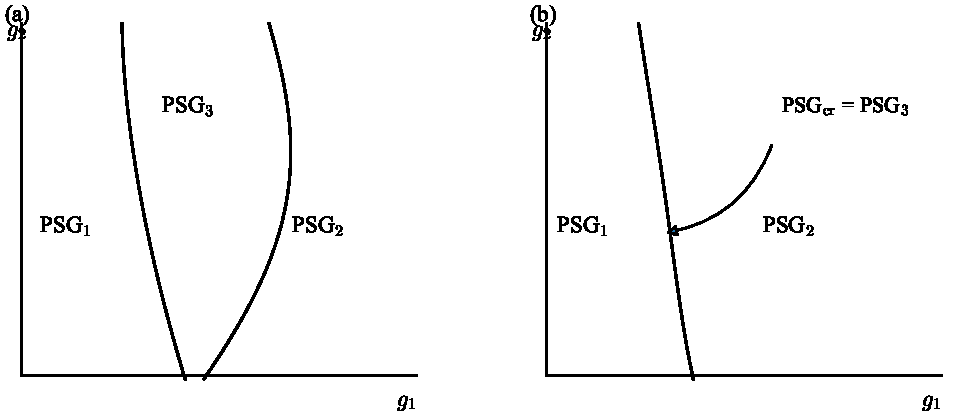
\includegraphics[width=0.72\textwidth]{fig_9.7.pdf}
\caption*{图 9.7\quad (a) 由 $PSG_{1,2,3}$ 刻画三个相的平均场相图，它们之间的平均场相变是连续的。PSG 满足 $PSG_{1}\subset PSG_{3}$ 与 $PSG_{2}\subset PSG_{3}$。$PSG_{1,2,3}$ 的一种可能取法是 $PSG_{1}=$Z2A0013、$PSG_{2}=$Z2Azz13、$PSG_{3}=$U1Cn01n。(b) 计入量子涨落后相应的物理相图。这里我们假定，计入量子涨落之后，态 $PSG_{3}$ 变成一个只带一个相关微扰的不稳定不动点。平均场态 $PSG_{3}$ 收缩成一条临界线，它描述两个态 $PSG_{1}$ 与 $PSG_{2}$ 之间的相变。交错通量态 U1Cn01n 如果不稳定，可能作为一个临界态出现。}
\end{figure}

我们想强调，上述所有自旋液体都具有相同的对称性。因此，它们之间的连续相变（如果存在的话）代表了一类新的量子连续相变——不改变任何对称性的相变（Wegner, 1971; Kosterlitz and Thouless, 1973; Dasgupta and Halperin, 1981; Wen and Wu, 1993; Chen \emph{et al.}, 1993; Senthil \emph{et al.}, 1999; Read and Green, 2000; Wen, 2000）。

\subsection*{问题 9.5.1}

拟设
\begin{equation*}
\begin{array}{rcl}
u_{\pmb{i},\pmb{i}+\pmb{x}}=\chi\tau^{1}-\eta\tau^{2}, & & u_{\pmb{i},\pmb{i}+\pmb{y}}=\chi\tau^{1}+\eta\tau^{2},\qquad a_{0}^{1,2,3}=0,\\[2pt]
u_{\pmb{i},\pmb{i}+2\pmb{x}+\pmb{y}}=u_{\pmb{i},\pmb{i}-\pmb{x}+2\pmb{y}}=+\lambda\tau^{3}, & & u_{\pmb{i},\pmb{i}+2\pmb{x}-\pmb{y}}=u_{\pmb{i},\pmb{i}+\pmb{x}+2\pmb{y}}=-\lambda\tau^{3},
\end{array}
\end{equation*}
在 $\chi\neq\eta$ 时，$\lambda=0$ 的情形描述 U1Cn01n 自旋液体（交错通量态）。
\begin{enumerate}
\item 证明：当 $\lambda\neq0$ 时，该拟设描述一个 $Z_{2}$ 自旋液体。
\item 找出保持该拟设不变的 U1Cn01n PSG 的子群。
\item 找出上述 $Z_{2}$ 拟设的标记。
\end{enumerate}

\section{对称自旋液体动物园}

\begin{keypoints}
\item 交错通量态邻域中 8 个 $Z_{2}$ 自旋液体的物理性质。
\end{keypoints}

本节中，我们想研究 9.4 节所分类的对称自旋液体的物理性质。我们一直用投影对称性来刻画不同的平均场态。然而，从一个平均场态的 PSG 直接看出它的物理性质并不容易。为了找出平均场态的物理性质，我们需要构造在相应 PSG 下不变的显式拟设。

然而，把几百个对称自旋液体一一列出绝非易事，更不用说逐一构造它们的拟设并研究其理论性质了。我们这里想做的是研究一些重要的自旋液体；可是，如何判定一个自旋液体的重要性呢？

在对高 $T_{c}$ 超导体的研究中，人们发现 $SU(2)$ 线性态 SU2Bn0（$\pi$ 通量态）、$U(1)$ 线性态 U1Cn01n（交错通量/$d$ 波态）与 $SU(2)$ 无能隙态 SU2An0（均匀 RVB 态）是重要的。它们与高 $T_{c}$ 超导体中观察到的某些相密切相关。$SU(2)$ 线性态、$U(1)$ 线性态与 $SU(2)$ 无能隙态分别再现了未掺杂、欠掺杂与过掺杂样品中观察到的电子谱函数。然而在理论上，由于 $U(1)$ 或 $SU(2)$ 规范涨落，这些自旋液体在低能下是不稳定的。这些态可能会变为它们邻域中更稳定的自旋液体。这促使我们研究 $SU(2)$ 线性态、$U(1)$ 线性态与 $SU(2)$ 无能隙态邻域中这些更稳定的自旋液体。为了进一步缩小范围，本节将主要研究 $U(1)$ 线性态 U1Cn01n 邻域中的自旋液体。\footnote{我们想指出，这里我们只研究对称自旋液体。U1Cn01n 自旋液体也可能变为其他一些破缺某些对称性的态。这样的对称性破缺相变实际上已经在高 $T_{c}$ 超导体中被观察到（如向反铁磁态、$d$ 波超导态与条纹态的转变）。}

\subsection{$U(1)$ 线性自旋液体周围的对称自旋液体}

U1Cn01n 自旋液体 (9.2.34) 可以连续变为 8 个不同的自旋液体，它们把 $U(1)$ 规范结构破缺到 $Z_{2}$ 规范结构。这 8 个自旋液体尽管都具有相同的对称性，却由不同的 PSG 标记。下面我们将更详细地研究这 8 个 $Z_{2}$ 自旋液体。特别地，我们想求出它们之中的自旋子谱。

第一个以 Z2A0013 标记，具有如下形式：
\begin{equation*}
\begin{array}{rcl}
u_{\pmb{i},\pmb{i}+\pmb{x}}=\chi\tau^{1}-\eta\tau^{2}, & & u_{\pmb{i},\pmb{i}+\pmb{y}}=\chi\tau^{1}+\eta\tau^{2},\\[2pt]
u_{\pmb{i},\pmb{i}+\pmb{x}+\pmb{y}}=+\gamma\tau^{1}, & & u_{\pmb{i},\pmb{i}-\pmb{x}+\pmb{y}}=+\gamma\tau^{1},\\[2pt]
a_{0}^{1}\neq0,\qquad a_{0}^{2,3}=0. & &
\end{array}
\tag{9.6.1}
\end{equation*}
它与拟设 (9.2.41) 具有相同的量子序。标记 Z2A0013 告诉我们该拟设的 PSG——即它的“对称性”群。提醒一下，对称自旋液体的 PSG 由对称性变换与规范变换的复合 $\{G_{0},\allowbreak\,G_{x}T_{x},\allowbreak\,G_{y}T_{y},\allowbreak\,G_{P_{x}}P_{x},\allowbreak\,G_{P_{y}}P_{y},\allowbreak\,G_{P_{xy}}P_{xy},\allowbreak\,G_{T}T\}$ 生成。规范变换 $G_{0}$ 生成该 PSG 的 IGG。标记中的“Z2”告诉我们 IGG 为 $Z_{2}$ 且 $G_{0}(\pmb{i})=(-)$；“A”告诉我们 $G_{x}(\pmb{i})=G_{y}(\pmb{i})=1$；接下来的“00”意味着 $G_{P_{x}}(\pmb{i})=1$、$G_{P_{y}}(\pmb{i})=1$；“1”意味着 $G_{P_{xy}}(\pmb{i})=\mathrm{i}\tau^{1}$，而“3”意味着 $G_{T}(\pmb{i})=\mathrm{i}\tau^{3}$。第二个拟设以 Z2Azz13 标记，具有如下形式：
\begin{equation*}
\begin{array}{rcl}
u_{\pmb{i},\pmb{i}+\pmb{x}}=\chi\tau^{1}-\eta\tau^{2}, & & u_{\pmb{i},\pmb{i}+\pmb{y}}=\chi\tau^{1}+\eta\tau^{2},\\[2pt]
u_{\pmb{i},\pmb{i}+\pmb{x}+\pmb{y}}=-\gamma\tau^{1}, & & u_{\pmb{i},\pmb{i}-\pmb{x}+\pmb{y}}=+\gamma\tau^{1},\\[2pt]
u_{\pmb{i},\pmb{i}+2\pmb{x}}=u_{\pmb{i},\pmb{i}+2\pmb{y}}=0,\qquad a_{0}^{1,2,3}=0. & &
\end{array}
\tag{9.6.2}
\end{equation*}
现在标记中的“zz”告诉我们 $\eta_{xpx}=\eta_{xpy}=-1$，$g_{P_{x}}=g_{P_{y}}=\mathrm{i}\tau^{3}$，于是 $G_{P_{x}}(\pmb{i})=(-)^{i_{x}+i_{y}}\tau^{3}$、$G_{P_{y}}(\pmb{i})=(-)^{i_{x}+i_{y}}\tau^{3}$（见式 (9.4.14)）。第三个拟设以 Z2A001n 标记，具有如下形式：
\begin{equation*}
\begin{array}{rcl}
a_{0}^{l}=0, & & \\[2pt]
u_{\pmb{i},\pmb{i}+\pmb{x}}=\chi\tau^{1}+\eta\tau^{2}, & & u_{\pmb{i},\pmb{i}+\pmb{y}}=\chi\tau^{1}-\eta\tau^{2}\\[2pt]
u_{\pmb{i},\pmb{i}+2\pmb{x}+\pmb{y}}=\chi_{1}\tau^{1}+\eta_{1}\tau^{2}+\lambda_{1}\tau^{3}, & & u_{\pmb{i},\pmb{i}-\pmb{x}+2\pmb{y}}=\chi_{1}\tau^{1}-\eta_{1}\tau^{2}-\lambda_{1}\tau^{3},\\[2pt]
u_{\pmb{i},\pmb{i}+2\pmb{x}-\pmb{y}}=\chi_{1}\tau^{1}+\eta_{1}\tau^{2}+\lambda_{1}\tau^{3}, & & u_{\pmb{i},\pmb{i}+\pmb{x}+2\pmb{y}}=\chi_{1}\tau^{1}-\eta_{1}\tau^{2}-\lambda_{1}\tau^{3}.
\end{array}
\tag{9.6.3}
\end{equation*}
如果你足够细心，就会发现标记 Z2A001n 并不出现在 9.4.3 节所分类的 196 个 $Z_{2}$ 自旋液体的名单之中（见表 9.1）。不过，以 Z2A001n 标记的 PSG 与以 Z2A003n 标记的 PSG 是规范等价的，而 Z2A003n 确实出现在名单中（见表 9.1 第二行）。下面我们将把上述自旋液体称为 Z2A003n 态。第四个拟设以 Z2Azz1n 标记，具有如下形式：
\begin{equation*}
\begin{array}{rcl}
a_{0}^{l}=0, & & \\[2pt]
u_{\pmb{i},\pmb{i}+\pmb{x}}=\chi\tau^{1}+\eta\tau^{2}, & & u_{\pmb{i},\pmb{i}+\pmb{y}}=\chi\tau^{1}-\eta\tau^{2}\\[2pt]
u_{\pmb{i},\pmb{i}+2\pmb{x}+\pmb{y}}=\chi_{1}\tau^{1}+\eta_{1}\tau^{2}+\lambda\tau^{3}, & & u_{\pmb{i},\pmb{i}-\pmb{x}+2\pmb{y}}=\chi_{1}\tau^{1}-\eta_{1}\tau^{2}+\lambda\tau^{3},\\[2pt]
u_{\pmb{i},\pmb{i}+2\pmb{x}-\pmb{y}}=\chi_{1}\tau^{1}+\eta_{1}\tau^{2}-\lambda\tau^{3}, & & u_{\pmb{i},\pmb{i}+\pmb{x}+2\pmb{y}}=\chi_{1}\tau^{1}-\eta_{1}\tau^{2}-\lambda\tau^{3}.
\end{array}
\tag{9.6.4}
\end{equation*}

上面四个拟设具有平移不变性。接下来四个 $Z_{2}$ 拟设不具有平移不变性，因为它们都是 Z2B 型的。（不过，投影之后它们仍然描述平移对称的自旋液体。）这些 $Z_{2}$ 自旋液体如下：

Z2B0013：
\begin{equation*}
\begin{array}{rcl}
u_{\pmb{i},\pmb{i}+\pmb{x}}=\chi\tau^{1}-\eta\tau^{2}, & & u_{\pmb{i},\pmb{i}+\pmb{y}}=(-)^{i_{x}}(\chi\tau^{1}+\eta\tau^{2}),\\[2pt]
u_{\pmb{i},\pmb{i}+2\pmb{x}}=-\gamma_{2}\tau^{1}+\lambda_{2}\tau^{2}, & & u_{\pmb{i},\pmb{i}+2\pmb{y}}=-\gamma_{2}\tau^{1}-\lambda_{2}\tau^{2},\\[2pt]
a_{0}^{1}\neq0,\qquad a_{0}^{2,3}=0, & &
\end{array}
\tag{9.6.5}
\end{equation*}

Z2Bzz13：
\begin{equation*}
\begin{array}{rcl}
u_{\pmb{i},\pmb{i}+\pmb{x}}=\chi\tau^{1}-\eta\tau^{2}, & & u_{\pmb{i},\pmb{i}+\pmb{y}}=(-)^{i_{x}}(\chi\tau^{1}+\eta\tau^{2}),\\[2pt]
u_{\pmb{i},\pmb{i}+2\pmb{x}+2\pmb{y}}=-\gamma_{1}\tau^{1}, & & u_{\pmb{i},\pmb{i}-2\pmb{x}+2\pmb{y}}=\gamma_{1}\tau^{1},\\[2pt]
a_{0}^{1,2,3}=0, & &
\end{array}
\tag{9.6.6}
\end{equation*}

Z2B001n：
\begin{equation*}
\begin{array}{rcl}
u_{\pmb{i},\pmb{i}+\pmb{x}}=\chi\tau^{1}+\eta\tau^{2}, & & u_{\pmb{i},\pmb{i}+\pmb{y}}=(-)^{i_{x}}(\chi\tau^{1}-\eta\tau^{2}),\\[2pt]
u_{\pmb{i},\pmb{i}+2\pmb{x}+\pmb{y}}=(-)^{i_{x}}\lambda\tau^{3}, & & u_{\pmb{i},\pmb{i}-\pmb{x}+2\pmb{y}}=-\lambda\tau^{3},\\[2pt]
u_{\pmb{i},\pmb{i}+2\pmb{x}-\pmb{y}}=(-)^{i_{x}}\lambda\tau^{3}, & & u_{\pmb{i},\pmb{i}+\pmb{x}+2\pmb{y}}=-\lambda\tau^{3},\\[2pt]
a_{0}^{l}=0, & &
\end{array}
\tag{9.6.7}
\end{equation*}

以及 Z2Bzz1n：
\begin{equation*}
\begin{array}{rcl}
u_{\pmb{i},\pmb{i}+\pmb{x}}=\chi\tau^{1}+\eta\tau^{2}, & & u_{\pmb{i},\pmb{i}+\pmb{y}}=(-)^{i_{x}}(\chi\tau^{1}-\eta\tau^{2}),\\[2pt]
u_{\pmb{i},\pmb{i}+2\pmb{x}+\pmb{y}}=(-)^{i_{x}}(\chi_{1}\tau^{1}+\eta_{1}\tau^{2}+\lambda\tau^{3}), & & u_{\pmb{i},\pmb{i}-\pmb{x}+2\pmb{y}}=\chi_{1}\tau^{1}-\eta_{1}\tau^{2}+\lambda\tau^{3},\\[2pt]
u_{\pmb{i},\pmb{i}+2\pmb{x}-\pmb{y}}=(-)^{i_{x}}(\chi_{1}\tau^{1}+\eta_{1}\tau^{2}-\lambda\tau^{3}), & & u_{\pmb{i},\pmb{i}+\pmb{x}+2\pmb{y}}=\chi_{1}\tau^{1}-\eta_{1}\tau^{2}-\lambda\tau^{3},\\[2pt]
a_{0}^{l}=0. & &
\end{array}
\tag{9.6.8}
\end{equation*}

对于式 (9.6.1)、(9.6.2)、(9.6.3) 与 (9.6.4) 给出的前四个 $Z_{2}$ 自旋液体（假定式 (9.6.1) 中 $a_{0}^{1}$ 较小），自旋子在四个孤立点处无能隙，并具有线性色散（见图 9.8）。因此，这四个拟设描述对称的 $Z_{2}$ 线性自旋液体。第二个 $Z_{2}$ 自旋液体 Z2Azz13 的单自旋子（single-spinon）色散相当有趣：它不具有 $90^{\circ}$ 旋转对称性。这与基态中的 $90^{\circ}$ 对称性并不矛盾，因为奇数个自旋子的激发永远无法满足约束，因而是被禁止的。自旋子色散具有绕 $\pmb{k}=(0,\pi)$ 的 $90^{\circ}$ 旋转对称性，而偶数个自旋子的激发谱则具有 $90^{\circ}$ 旋转对称性。

\begin{figure}[H]
\centering
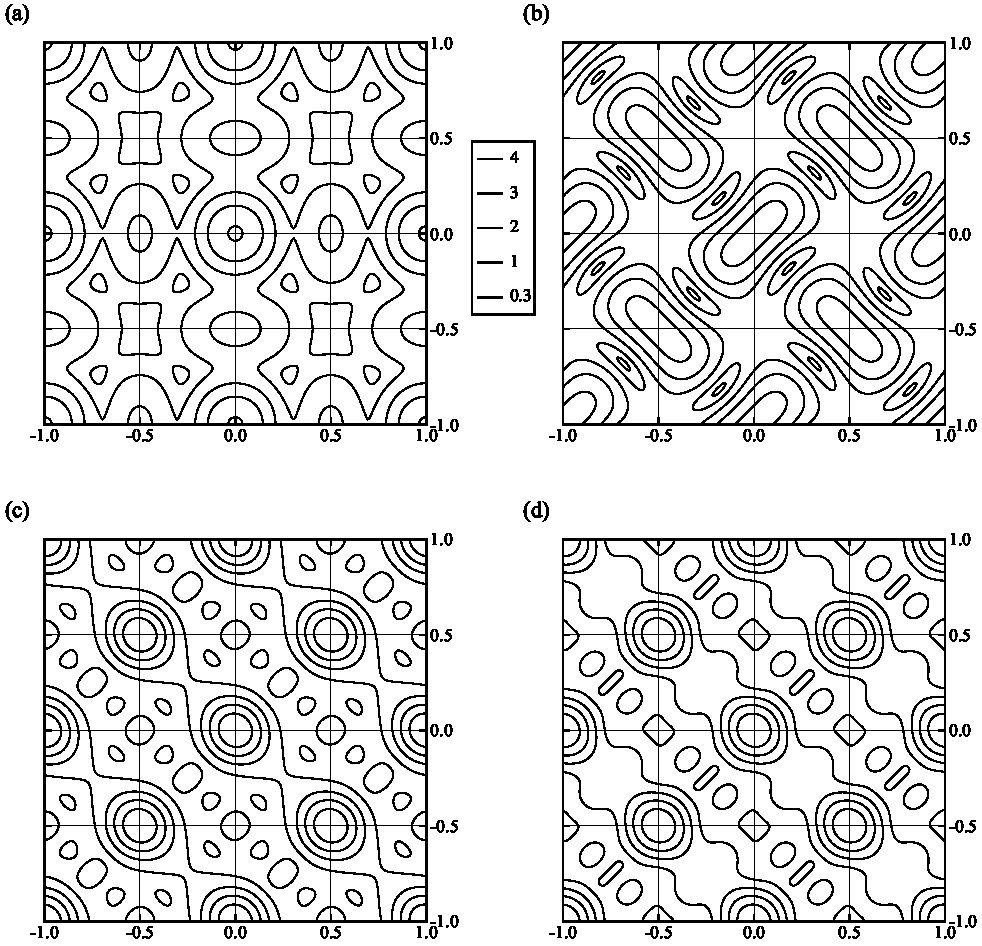
\includegraphics[width=0.72\textwidth]{fig_9.8.pdf}
\caption*{图 9.8\quad $Z_{2}$ 线性自旋液体的自旋子色散 $E_{+}(\pmb{k})$ 作为 $(k_{x}/2\pi,\,k_{y}/2\pi)$ 的函数的等高线图：(a) 式 (9.6.1) 的 Z2A0013 态；(b) 式 (9.6.2) 的 Z2Azz13 态；(c) 式 (9.6.3) 的 Z2A001n 态；(d) 式 (9.6.4) 的 Z2Azz1n 态。}
\end{figure}

我们想指出，当 $a_{0}^{1}$ 较大时，式 (9.6.1) 可能有有能隙的自旋子谱。因此，Z2A0013 态既可能是有能隙自旋液体，也可能是无能隙自旋液体。其余三个 Z2A 态总是无能隙的，是 $Z_{2}$ 线性态。在 9.9 节中我们将证明，所有 $Z_{2}$ 有能隙态与 $Z_{2}$ 线性态都是稳定的。这些态的平均场结果可以应用于物理自旋液体。

接下来让我们考虑式 (9.6.5) 中的拟设 Z2B0013。拟设 (9.6.5) 的自旋子谱由下式的本征值确定：
\begin{equation*}
H=-2\big[\chi\cos(k_{x})\Gamma_{0}-\eta\cos(k_{x})\Gamma_{2}-\chi\cos(k_{y})\Gamma_{1}+\eta\cos(k_{y})\Gamma_{3}\big]+\lambda\Gamma_{4}
\end{equation*}

\begin{figure}[H]
\centering
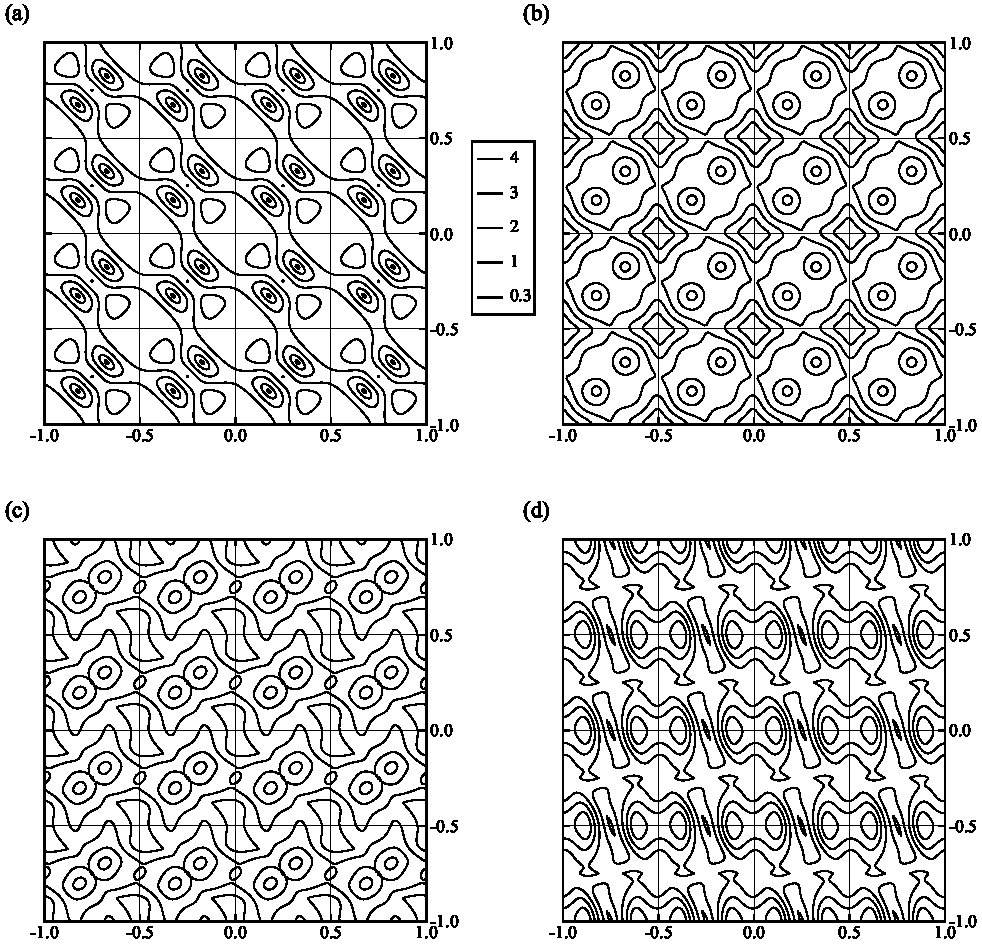
\includegraphics[width=0.72\textwidth]{fig_9.9.pdf}
\caption*{图 9.9\quad $Z_{2}$ 线性态的自旋子色散 $\min(E_{1}(\pmb{k}),E_{2}(\pmb{k}))$ 作为 $(k_{x}/2\pi,\,k_{y}/2\pi)$ 的函数的等高线图：(a) 式 (9.6.5) 的 Z2B0013 态；(b) 式 (9.6.6) 的 Z2Bzz13 态；(c) 式 (9.6.7) 的 Z2B001n 态；(d) 式 (9.6.8) 的 Z2Bzz1n 态。}
\end{figure}

其中 $k_{x}\in(0,\pi)$，$k_{y}\in(-\pi,\pi)$，而
\begin{equation*}
\begin{array}{rcl}
\Gamma_{0}=\tau^{1}\otimes\tau^{3}, & \quad\Gamma_{1}=\tau^{1}\otimes\tau^{1}, & \quad\Gamma_{2}=\tau^{2}\otimes\tau^{3},\\[2pt]
\Gamma_{3}=\tau^{2}\otimes\tau^{1}, & \quad\Gamma_{4}=\tau^{1}\otimes\tau^{0}, &
\end{array}
\end{equation*}
这里已取 $\gamma_{1,2}=\lambda_{2}=0$。自旋子色散的四支能带具有 $\pm E_{1}(\pmb{k})$、$\pm E_{2}(\pmb{k})$ 的形式。我们发现自旋子谱在 $\pmb{k}=(\pi/2,\pm\pi/2)$ 附近的 8 个孤立点处为零（见图 9.9(a)）。因此，Z2B0013 态是一个 $Z_{2}$ 线性自旋液体。

其余三个 Z2B 态的自旋子谱可以用类似方法求出，谱图画在图 9.9 中。这三个 Z2B 态也是 $Z_{2}$ 线性态。无能隙自旋子只出现在 $\big(\frac{\pi}{2},\pm\frac{\pi}{2}\big)$ 处。

% ---------------- 新增术语（ch9_e） ----------------
% | staggered-flux phase | 交错通量相（ch9_c 已收 staggered-flux state 交错通量态） |
% | U(1)/SU(2) projective symmetry group | U(1)/SU(2) 投影对称群（= U(1)/SU(2) PSG） |
% | type-U1A/U1B/U1C PSG | U1A/U1B/U1C 型 PSG |
% | label (of a PSG) | 标记（PSG 的标记） |
% | quantum critical state | 量子临界态 |
% | critical line | 临界线 |
% | unstable fixed point | 不稳定不动点 |
% | destabilize | 使……失稳 |
% | single-spinon (excitation/spectrum) | 单自旋子（激发/谱） |
% | non-collinear flux | 非共线通量（collinear 共线的，术语表已收） |
% | contour plot | 等高线图 |
% | the zoo of ... | ……动物园（章节名修辞，照译） |

% 块边界判定：
%   起点——书页 419（p434）首段 "Knowing the translational symmetry ..." 为完整新句；
%     前块止于书页 418 末 "The gapless spinons appear only at (pi/2, +/-pi/2)."，
%     无前块溢出内容，故本块不设 %JOIN%，亦无需 TAIL 区。
%   实际覆盖——书页 419 起于 9.6.1 节后部（式 (9.6.9) 之前的段落），依次为 9.6.2 节、
%     9.7 节、9.8 节（含 9.8.1、9.8.2）、9.9 节引言；9.5 节与 9.6/9.6.1 节标题、
%     式 (9.6.1)--(9.6.8)、图 9.8、图 9.9 均在前块（书页 415--418）内。
%   终点——书页 430（p445）末句 "... in the light of quantum orders and their PSG
%     characterization." 为 9.9 节引言末句，书页 431（p446）顶部起新小节 9.9.1，
%     本块自然收尾，不设 %--E-TAIL--。
% 蓝本问题记录：
%   1) 问题 9.6.3(a) 原书把 eta/chi 与两个态的对应关系印反（与 9.6.2 节正文矛盾：
%      正文为 chi=0 -> SU2An0、eta=0 -> SU2Bn0，与拟设形式逐项比对一致），
%      且将 SU2Bn0 误标为 "SU(2)-gapless"，已按正文与本意订正并加译注。
%   2) 式 (9.8.9) 末行原书漏印下标 0（作 $a^{1,2}=0$），按本意作 $a_0^{1,2}=0$。
%   3) 式 (9.6.9) 原书即印作 $k_1+k_2+\pi x$（而变换式为 $|\pmb{k}\rangle\to
%      |\pmb{k}+\pi\pmb{y}\rangle$），照原图转写。
%   4) 图 9.10 图注 "the two-spinon spectrum docs have" 中 "docs" 为 "does" 之误。

\begin{figure}[H]
\centering
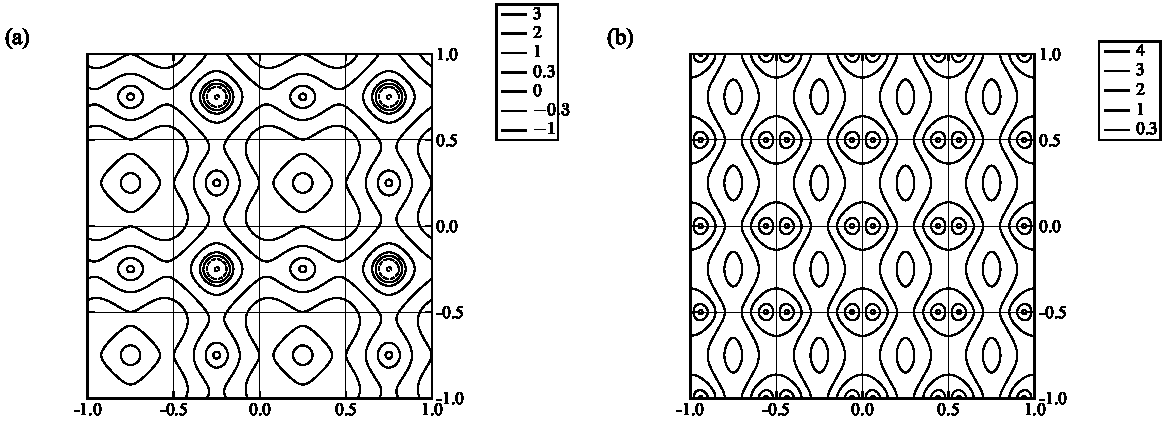
\includegraphics[width=0.72\textwidth]{fig_9.10.pdf}
\caption*{图 9.10\quad $Z_2$ 自旋液体自旋子色散 $E_+(\pmb{k})$ 作为 $(k_x/2\pi,\,k_y/2\pi)$ 的函数的等高线图：(a) 式 (9.2.39) 中的 $Z_2$ 无能隙态 Z2Ax2(12)n；(b) 式 (9.6.10) 中的 $Z_2$ 二次方态 Z2Bx2(12)n。尽管 (a) 中的单自旋子色散缺乏旋转对称性和宇称对称性，双自旋子谱却具有这些对称性。}
\end{figure}

虽然上述 Z2B 自旋液体具有平移对称性，但发现自旋子谱只在格点布里渊区的一半上有定义，这一点看起来很奇怪。不过，这与物理自旋液体中的平移对称性并不矛盾，因为单自旋子激发并不是物理的。只有双自旋子激发才对应于物理激发，其谱应当定义在满布里渊区上。现在的问题是：如何从只在半布里渊区上有定义的单自旋子谱，得到定义在满布里渊区上的双自旋子谱。设 $|\pmb{k},1\rangle$ 与 $|\pmb{k},2\rangle$ 是单自旋子的两个本征态，能量为正，分别为 $E_1(\pmb{k})$ 与 $E_2(\pmb{k})$（这里 $k_x\in(-\pi/2,\pi/2)$，$k_y\in(-\pi,\pi)$）。沿 $\pmb{x}$ 的平移（随后再作一个规范变换）把 $|\pmb{k},1\rangle$ 与 $|\pmb{k},2\rangle$ 变成能量相同的另外两个本征态：
\begin{equation*}
\begin{aligned}
|\pmb{k},1\rangle &\to |\pmb{k}+\pi\pmb{y},1\rangle \\
|\pmb{k},2\rangle &\to |\pmb{k}+\pi\pmb{y},2\rangle
\end{aligned}
\end{equation*}
于是我们看到，双自旋子态 $|\pmb{k}_1,\alpha_1\rangle|\pmb{k}_2,\alpha_2\rangle\pm|\pmb{k}_1+\pi\pmb{y},\alpha_1\rangle|\pmb{k}_2+\pi\pmb{y},\alpha_2\rangle$ 的动量与能量由下式给出：
\begin{equation*}
\begin{aligned}
E_{2\text{-spinon}} &= E_{\alpha_1}(\pmb{k}_1)+E_{\alpha_2}(\pmb{k}_2) \\
\pmb{k} &= \pmb{k}_1+\pmb{k}_2,\ \ \pmb{k}_1+\pmb{k}_2+\pi\pmb{x}
\end{aligned}
\tag{9.6.9}
\end{equation*}
式 (9.6.9) 使我们能够由单自旋子谱构造出双自旋子谱。

\subsection{$SU(2)$ 自旋液体附近的一个奇怪的对称自旋液体}

在式 (9.2.32) 的均匀 RVB 态（即 $SU(2)$ 无能隙态 SU2An0）附近以及式 (9.2.33) 的 $\pi$ 通量态（即 $SU(2)$ 线性态 SU2Bn0）附近，存在许多类型的对称拟设。这里我们只考虑其中的一个——$Z_2$ 自旋液体 Z2By1(12)n（注意 Z2By1(12)n 与 Z2Bx2(12)n 规范等价），它具有如下形式：
\begin{equation*}
u_{\pmb{i},\pmb{i}+\pmb{x}}=\mathrm{i}\chi\tau^{0}+\eta\tau^{1},\qquad
u_{\pmb{i},\pmb{i}+\pmb{y}}=(-)^{i_x}(\mathrm{i}\chi\tau^{0}+\eta\tau^{2}),\qquad
a_0^{1,2,3}=0.
\tag{9.6.10}
\end{equation*}
上述拟设在 $\chi=0$ 时退化为 $SU(2)$ 无能隙态 SU2An0 的拟设，在 $\eta=0$ 时退化为 $SU(2)$ 线性态 SU2Bn0 的拟设。经过傅里叶变换，我们发现自旋子谱由下式决定：
\begin{equation*}
H=-2\chi\sin(k_x)\Gamma_0+2\eta\cos(k_x)\Gamma_2-2\chi\sin(k_y)\Gamma_1+2\eta\cos(k_y)\Gamma_3
\end{equation*}
其中 $k_x\in(-\pi/2,\pi/2)$，$k_y\in(-\pi,\pi)$，而
\begin{equation*}
\Gamma_0=\tau^{0}\otimes\tau^{3},\qquad
\Gamma_2=\tau^{1}\otimes\tau^{3},\qquad
\Gamma_1=\tau^{0}\otimes\tau^{1},\qquad
\Gamma_3=\tau^{2}\otimes\tau^{1}.
\end{equation*}
自旋子谱可以精确计算，它的四支具有 $\pm E_1(\pmb{k})$ 与 $\pm E_2(\pmb{k})$ 的形式。自旋子能量在两个孤立点 $\pmb{k}=(0,0)$ 与 $(0,\pi)$ 处为零。在 $\pmb{k}=0$ 附近，低能谱由下式给出（见图 9.10(b)）
\begin{equation*}
E=\pm\eta^{-1}\sqrt{(\chi^{2}+\eta^{2})^{2}(k_x^{2}-k_y^{2})^{2}+4\chi^{4}k_x^{2}k_y^{2}}
\end{equation*}
有趣（而且奇怪）的是，当 $\pmb{k}\to 0$ 时能量并不线性地趋于零，而是像 $k^{2}$ 那样趋于零！为了强调这种 $E\propto k^{2}$ 的二次方色散，我们将把这样的态称为 $Z_2$ 二次方自旋液体（$Z_2$-quadratic spin liquid）。

\subsection*{问题 9.6.1}

拟设 (9.6.3) 的 PSG。
\begin{enumerate}
\item 试由标记 Z2A001n 求出 Z2A001n PSG 的规范变换 $G_x$、$G_y$、$G_{P_x}$ 等。
\item 证明拟设 (9.6.3) 在 Z2A001n PSG 下不变。
\item 试求把 Z2A001n PSG 变换到 Z2A003n PSG 的规范变换。
\end{enumerate}

\subsection*{问题 9.6.2}

验证：对于由式 (9.6.10) 描述的自旋液体，只要 $\chi$ 与 $\eta$ 都不为零，绕回路 $\pmb{i}\to\pmb{i}+\pmb{x}\to\pmb{i}+\pmb{x}+\pmb{y}\to\pmb{i}+\pmb{y}\to\pmb{i}$ 与 $\pmb{i}\to\pmb{i}+\pmb{y}\to\pmb{i}-\pmb{x}+\pmb{y}\to\pmb{i}-\pmb{x}\to\pmb{i}$ 的 $SU(2)$ 通量算符（见式 (9.2.20)）就互不对易。因此，该自旋液体确实具有 $Z_2$ 规范结构。

\subsection*{问题 9.6.3}

(a) 证明：当 $\eta=0$ 时，式 (9.6.10) 中的拟设退化为 $SU(2)$ 线性态 SU2Bn0 的拟设；当 $\chi=0$ 时，退化为 $SU(2)$ 无能隙态 SU2An0 的拟设。（译注：原书此句将 $\eta$、$\chi$ 与两个态的对应关系印反，且把 SU2Bn0 误标为 “$SU(2)$-gapless”，现按 9.6.2 节正文及物理内容订正。）

(b) 试求自旋子谱 $\pm E_1$ 与 $\pm E_2$。

\section{量子序的物理测量}

\begin{keypoints}
\item 用 PSG 描述的量子序可以通过激发谱来测量。
\end{keypoints}

在用 PSG 从数学上刻画了量子序之后，我们想问：如何在实验中测量量子序？有能隙态中的量子序与拓扑序相联系，我们可以用基态简并、边缘态、准粒子统计等手段来测量拓扑序（Wen, 1990, 1995; Senthil and Fisher, 2001）。具有无能隙激发的态中的量子序则需要用不同的方式来测量。在本节中，我们想证明：一般而言，量子序可以通过无能隙激发的动力学性质来测量。然而，并非所有的动力学性质都是普适的。因此，在用无能隙激发来刻画并测量量子序之前，我们需要先甄别出无能隙激发的普适性质。量子序的 PSG 刻画使我们能够得到这些普适性质——我们只需找出具有同一 PSG 的所有拟设的无能隙激发所共有的性质。

为了演示上述想法，我们想研究双自旋子激发的谱。我们注意到，自旋子只能成对地产生，因此单自旋子谱不是物理的。我们还注意到，双自旋子谱中包含自旋 1 激发，而自旋 1 激发可以用中子散射实验来测量。

在给定动量处，双自旋子谱分布在一段或几段能量范围内。设 $E_{2s}(\pmb{k})$ 为动量 $\pmb{k}$ 处双自旋子谱的低边缘。在平均场理论中，双自旋子谱可以由单自旋子色散按如下方式构造：
\begin{equation*}
E_{2\text{-spinon}}(\pmb{k})=E_{1\text{-spinon}}(\pmb{q})+E_{1\text{-spinon}}(\pmb{k}-\pmb{q})
\end{equation*}
在图 9.11--9.14 中，我们给出了几个简单自旋液体的平均场 $E_{2s}$。如果平均场态对规范涨落是稳定的，我们预计平均场 $E_{2s}$ 应当与真实的 $E_{2s}$ 在定性上一致。

在我们的例子中，有八个稳定的 $Z_2$ 线性自旋液体（见图 9.11 与 9.12）。以这八个 $Z_2$ 自旋液体为例，我们可以演示自旋 1 激发的普适性质如何区分不同的量子序。

\begin{figure}[H]
\centering
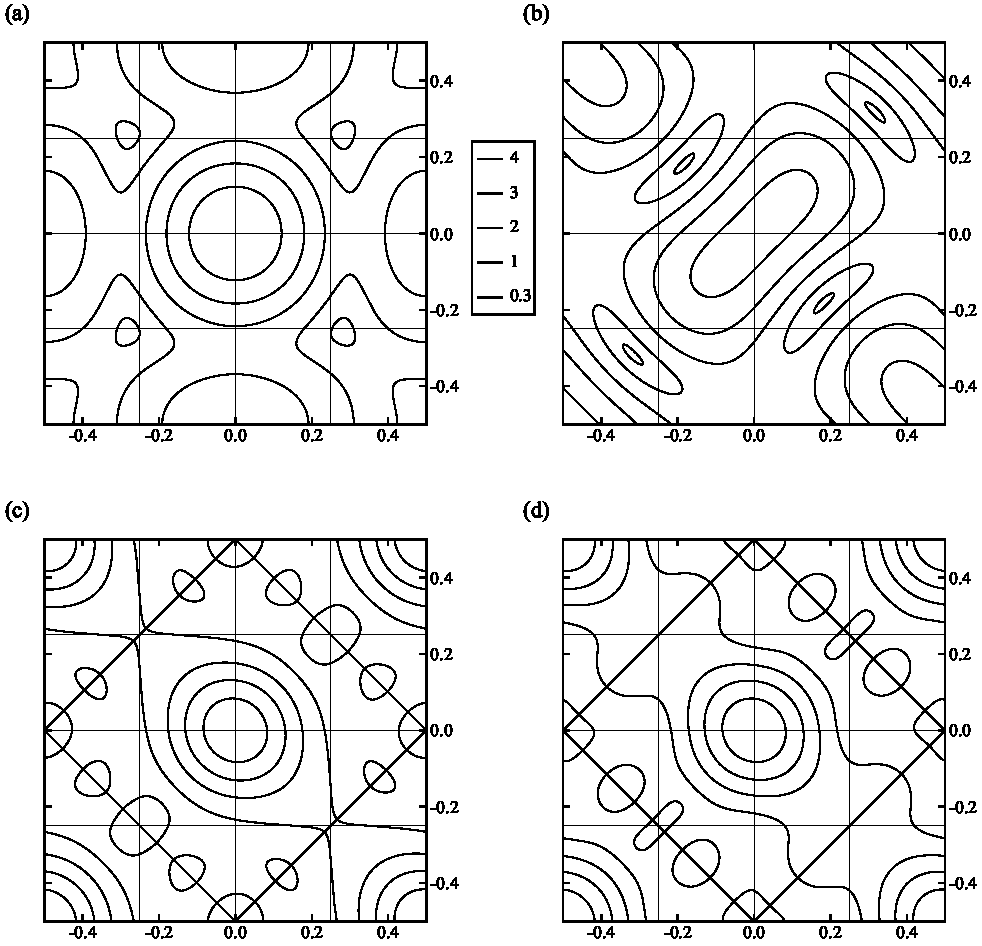
\includegraphics[width=0.72\textwidth]{fig_9.11.pdf}
\caption*{图 9.11\quad $Z_2$ 线性自旋液体的 $E_{2s}(\pmb{k})$ 作为 $(k_x/2\pi,\,k_y/2\pi)$ 的函数的等高线图：(a) 式 (9.6.1) 中的 Z2A0013 态；(b) 式 (9.6.2) 中的 Z2Azz13 态；(c) 式 (9.6.3) 中的 Z2A001n 态；(d) 式 (9.6.4) 中的 Z2Azz1n 态。}
\end{figure}

(a) 通过考察自旋 1 激发的谱，可以把 Z2A 自旋液体与 Z2B 自旋液体区分开。对于 Z2B 自旋液体，自旋 1 谱以布里渊区的四分之一为周期（即谱在 $k_x\to k_x+\pi$ 与 $k_y\to k_y+\pi$ 下不变）。与之相反，Z2A 自旋液体中的自旋 1 谱不具有这种周期性。

(b) 自旋 1 谱的周期性还可以把 Z2A0013 与 Z2Azz13 自旋液体同 Z2A001n 与 Z2Azz1n 自旋液体区分开。对于 Z2A001n 与 Z2Azz1n 自旋液体，自旋 1 谱以布里渊区的二分之一为周期（即谱在 $(k_x,k_y)\to(k_x+\pi,k_y+\pi)$ 下不变）。此外，Z2A001n 与 Z2Azz1n 自旋液体恰好在 $(\pi,\pi)$、$(\pi,0)$ 和 $(0,\pi)$ 处有无能隙自旋 1 激发。

(c) Z2A0013 与 Z2Azz13 自旋液体可以通过考察 $(\pi,0)$ 和 $(0,\pi)$ 附近的无能隙自旋 1 激发来区分。Z2Azz13 自旋液体中的无能隙自旋 1 激发位于区边界上。

\begin{figure}[H]
\centering
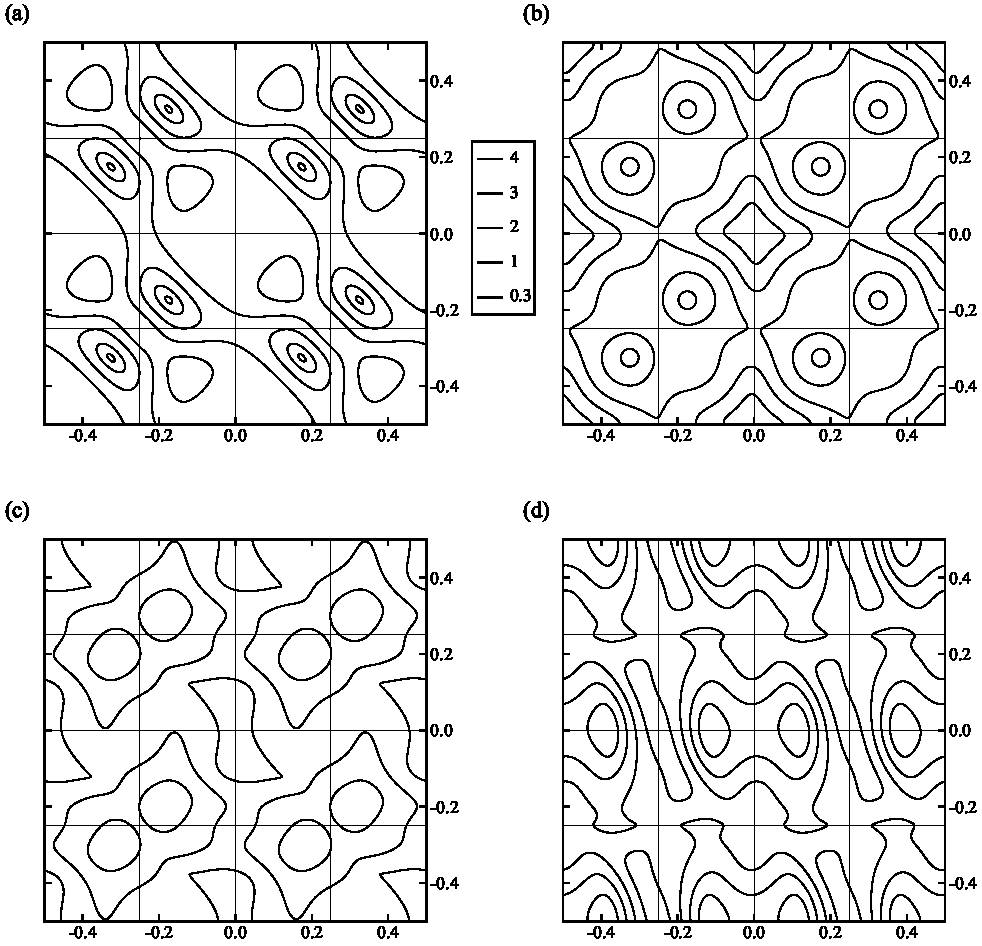
\includegraphics[width=0.72\textwidth]{fig_9.12.pdf}
\caption*{图 9.12\quad $Z_2$ 线性自旋液体的 $E_{2s}(\pmb{k})$ 作为 $(k_x/2\pi,\,k_y/2\pi)$ 的函数的等高线图：(a) 式 (9.6.5) 中的 Z2B0013 态；(b) 式 (9.6.6) 中的 Z2Bzz13 态；(c) 式 (9.6.7) 中的 Z2B001n 态；(d) 式 (9.6.8) 中的 Z2Bzz1n 态。谱以布里渊区的四分之一为周期。}
\end{figure}

我们看到，自旋液体中的量子序可以通过探测自旋 1 激发的中子散射实验来测量。

接下来，让我们讨论 $U(1)$ 线性态 U1Cn01n（交错通量态）。人们曾提出用 U1Cn01n 态描述欠掺杂高 $T_c$ 超导体中的赝能隙金属态（Wen and Lee, 1996; Rantner and Wen, 2001）。U1Cn01n 态自然地解释了欠掺杂金属态中的赝能隙。作为一种代数自旋液体，U1Cn01n 态还解释了赝能隙态中的类 Luttinger 电子谱函数（Rantner and Wen, 2001; Franz and Tesanovic, 2001）以及 $(\pi,\pi)$ 自旋涨落的增强（Kim and Lee, 1999; Rantner and Wen, 2002）。

\begin{figure}[H]
\centering
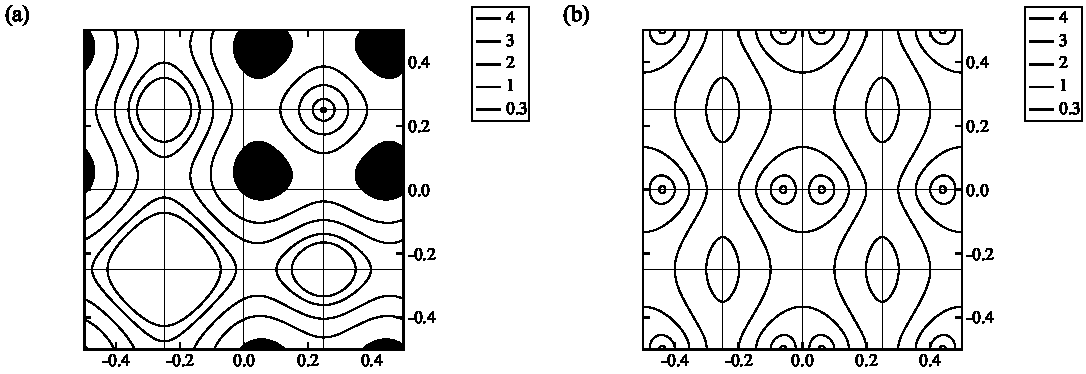
\includegraphics[width=0.72\textwidth]{fig_9.13.pdf}
\caption*{图 9.13\quad $E_{2s}(\pmb{k})$ 作为 $(k_x/2\pi,\,k_y/2\pi)$ 的函数的等高线图：(a) 式 (9.2.39) 中的 $Z_2$ 无能隙态 Z2Ax2(12)n；(b) 式 (9.6.10) 中的 $Z_2$ 二次方态 Z2Bx2(12)n。}
\end{figure}

\begin{figure}[H]
\centering
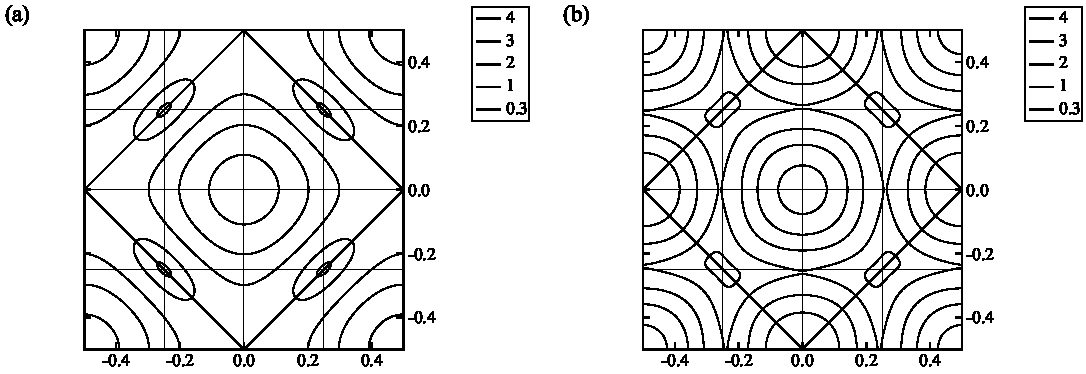
\includegraphics[width=0.72\textwidth]{fig_9.14.pdf}
\caption*{图 9.14\quad 两个 $U(1)$ 线性自旋液体的 $E_{2s}(\pmb{k})$ 作为 $(k_x/2\pi,\,k_y/2\pi)$ 的函数的等高线图：(a) 式 (9.2.34) 中的 U1Cn01n 态（交错通量相）；(b) 无能隙相中式 (9.8.9) 的 U1Cn00x 态。谱以布里渊区的二分之一为周期。}
\end{figure}

从图 9.14 我们看到，U1Cn01n 态中自旋 1 激发的无能隙点总是位于 $\pmb{k}=(\pi,\pi)$、$(0,0)$、$(\pi,0)$ 和 $(0,\pi)$。在所有这四个 $\pmb{k}$ 点处，自旋 1 连续谱边缘的等能线都具有两个彼此交叠的椭圆的形状。而且，等能线不垂直于区边界。所有这些都是 U1Cn01n 态的普适性质。在中子散射实验中测量这些性质，将使我们能够判断赝能隙金属态是否由 U1Cn01n（交错通量）态描述。

由于 $(2+1)$ 维 $U(1)$ 规范理论的瞬子效应，U1Cn01n 态是不稳定的。因此，U1Cn01n 态不得不变为其他一些态，例如 9.6 节中讨论的八个 $Z_2$ 自旋液体，或这里未讨论的其他态。从图 9.11(a) 我们看到，如果观察到 $(\pi,\pi)$ 处的节点劈裂为 $(\pi\pm\delta,\pi\pm\delta)$ 处的四个节点，以及 $(\pi,0)$ 和 $(0,\pi)$ 处的节点劈裂为 $(\pi\pm\delta,0)$ 和 $(0,\pi\pm\delta)$ 处的两个节点，就可以用中子散射探测从 U1Cn01n 态到 $Z_2$ 线性态 Z2A0013 的相变。从图 9.11(b) 我们看到，对于从 U1Cn01n 态到 $Z_2$ 线性态 Z2Azz13 的相变，$(\pi,\pi)$ 处的节点仍劈裂为 $(\pi\pm\delta,\pi\pm\delta)$ 处的四个节点，但 $(\pi,0)$ 和 $(0,\pi)$ 处的节点以另一种方式劈裂为 $(\pi,\pm\delta)$ 和 $(\pm\delta,\pi)$ 处的两个节点。我们还可以研究从 U1Cn01n 态到其余六个 $Z_2$ 自旋液体的相变。我们发现，自旋 1 激发谱以某些具有特征的方式改变。因此，通过测量自旋 1 激发谱及其演化，我们不仅能够探测不改变任何对称性的量子相变，还能够辨别正在发生的是哪一个相变。

\section{大 $N$ 极限下 $J_1$--$J_2$ 模型的相图}

\subsection{大 $N$ 极限}

\begin{keypoints}
\item 自旋-1/2 模型可以推广为 $SP(2N)$ 模型。
\item 对于 $SP(2N)$ 模型，由 $SU(2)$ 投影构造得到的平均场理论涨落微弱，是一个好的近似。
\end{keypoints}

到目前为止，我们一直集中讨论如何刻画、分类和测量不同的自旋液体及其量子序，还没有讨论如何寻找物理自旋哈密顿量，来实现我们构造的数百个不同自旋液体中的一些。本节就要处理这个问题。

在平均场层次上，设计一个实现具有给定量子序的自旋液体的自旋哈密顿量并不很难；对一个给定的自旋哈密顿量求出其平均场基态也不很难。真正的问题是我们是否应当相信平均场结果。我们已经看到，如果所得到的平均场基态是不稳定的（即如果平均场涨落导致低能下发散的相互作用），那么平均场结果不可信，平均场态不对应任何真实的物理自旋态。我们也曾论证过，如果平均场基态是稳定的（即平均场涨落导致低能下消失的相互作用），那么平均场结果可信，平均场态确实对应一个真实的物理自旋态。

这里我们想指出，上面关于稳定平均场态的论述过于乐观。一个“稳定平均场态”在低能下没有发散的涨落，所以它不一定不稳定；但另一方面，它也不一定稳定。这是因为短距离涨落如果足够强，同样会导致相变和失稳。因此，要使一个平均场结果可靠，平均场态必须稳定（或边缘），\emph{而且}短距离涨落必须微弱。由于我们的自旋模型中没有任何小参数，即便是稳定的平均场态，其短距离涨落也不微弱。正因如此，即使是稳定态的平均场结果能否应用于我们的自旋-1/2 模型，也并不清楚。

下面我们把自旋模型推广到大 $N$ 模型。我们将证明，大 $N$ 模型的平均场态具有微弱的短距离涨落，因此大 $N$ 模型的稳定与边缘平均场态对应于真实的物理态，稳定态或边缘态的平均场结果可以应用于大 $N$ 模型。

让我们从 $SU(2)$ 平均场理论的如下路径积分表示出发：
\begin{equation*}
\begin{aligned}
Z &= \int \mathcal{D}\psi\,\mathcal{D}[a_0^l(\pmb{i})]\,\mathcal{D}U_{ij}\ \mathrm{e}^{\mathrm{i}\int\mathrm{d}t\,(L-\sum_i a_0^l(\pmb{i},t)\psi_i^{\dagger}\tau^{l}\psi_i)} \\
L &= \sum_i \psi_i^{\dagger}\mathrm{i}\partial_t\psi_i-\sum_{\langle ij\rangle}\frac{1}{4}J_{ij}\left[\frac{1}{2}\mathrm{Tr}\,U_{ij}U_{ij}^{\dagger}-(\psi_i^{\dagger}U_{ij}\psi_j+h.c)\right].
\end{aligned}
\tag{9.8.1}
\end{equation*}
它由 $SU(2)$ 平均场哈密顿量 (9.2.9) 得到，其中 $U_{ij}$ 具有式 (9.2.13) 给出的形式。\footnote{我们把系数从 $3/8$ 改成了 $1/4$，这样，在式 (9.8.1) 中把 $U_{ij}$ 积掉就会得到自旋哈密顿量 (9.1.1)。}把费米子积掉之后，我们得到 $U_{ij}$ 与 $a_0^l$ 的有效拉格朗日量：
\begin{equation*}
Z=\int \mathcal{D}[a_0^l(\pmb{i})]\,\mathcal{D}U_{ij}\ \mathrm{e}^{\mathrm{i}\int\mathrm{d}t\,L_{0,eff}(U_{ij},a_0^l)}
\end{equation*}
问题在于，在上述路径积分中，$U_{ij}$ 与 $a_0^l$ 的涨落并不微弱。

为了减小涨落，我们引入 $N$ 份费米子副本 $\psi_i^a$，把式 (9.8.1) 推广为如下路径积分（Ran and Wen, 2003）：
\begin{equation*}
\begin{aligned}
Z &= \int \mathcal{D}\psi\,\mathcal{D}[a_0^l(\pmb{i})]\,\mathcal{D}U_{ij}\ \mathrm{e}^{\mathrm{i}\int\mathrm{d}t\,(L-\sum_i a_0^l(\pmb{i},t)\psi_i^{a\dagger}\tau^{l}\psi_i^{a})} \\
L &= \sum_i \psi_i^{a\dagger}\mathrm{i}\partial_t\psi_i^{a}-\sum_{\langle ij\rangle}\frac{1}{4}J_{ij}\left[\frac{N}{2}\mathrm{Tr}\,U_{ij}U_{ij}^{\dagger}-(\psi_i^{a\dagger}U_{ij}\psi_j^{a}+h.c)\right]
\end{aligned}
\tag{9.8.2}
\end{equation*}
其中 $a=1,2,\dots,N$。把费米子积掉之后，我们得到
\begin{equation*}
Z=\int \mathcal{D}[a_0^l(\pmb{i})]\,\mathcal{D}U_{ij}\ \mathrm{e}^{\mathrm{i}\int\mathrm{d}t\,N L_{0,eff}(U_{ij},a_0^l)}
\end{equation*}
我们看到，在大 $N$ 极限下，$U_{ij}$ 与 $a_0^l$ 的涨落是微弱的，平均场近似是一个好的近似。同样清楚的是，大 $N$ 平均场理论是一个 $SU(2)$ 规范理论，$U_{ij}$ 与 $a_0^l$ 的涨落对应于 $SU(2)$ 规范涨落。

在 9.2.1 节中，我们从物理自旋哈密顿量出发构造了平均场哈密顿量。这里我们面临的是相反的问题：已知大 $N$ 平均场哈密顿量
\begin{equation*}
H_{\text{mean}}=\sum_{\langle ij\rangle}\frac{1}{4}J_{ij}\left[\frac{N}{2}\mathrm{Tr}\,U_{ij}U_{ij}^{\dagger}-(\psi_i^{a\dagger}U_{ij}\psi_j^{a}+h.c)\right]+\sum_i a_0^l\psi_i^{a\dagger}\tau^{l}\psi_i^{a}
\tag{9.8.3}
\end{equation*}
我们想求出与之对应的物理的大 $N$ 自旋模型。

构造物理模型最重要的一步是找到物理希尔伯特空间。物理希尔伯特空间是费米子希尔伯特空间的一个子空间，由 $SU(2)$ 规范不变态、即满足约束
\begin{equation*}
\psi_i^{a\dagger}\tau^{l}\psi_i^{a}|phy\rangle,\qquad l=1,2,3
\end{equation*}
的态构成，且该约束在每个格点 $\pmb{i}$ 上都要成立。

得到每个格点上的物理希尔伯特空间之后，我们还需要找到在物理希尔伯特空间内部起作用的物理算符。这些物理算符是 $SU(2)$ 规范不变算符（即与 $\psi_i^{a\dagger}\tau^{l}\psi_i^{a}$ 对易的算符）。让我们把每个格点上 $\psi$ 的所有 $SU(2)$ 规范不变双线性型写下来：
\begin{equation*}
\begin{aligned}
S^{ab+}&\equiv\frac{1}{2}\psi_\alpha^{a\dagger}\tilde\psi_\alpha^{b},\qquad
S^{ab-}\equiv\frac{1}{2}\tilde\psi_\alpha^{a\dagger}\psi_\alpha^{b},\\
S^{ab3}&\equiv\frac{1}{2}\left(\psi_\alpha^{a\dagger}\psi_\alpha^{b}-\delta^{ab}\right)
=\frac{1}{2}\left(\delta^{ab}-\tilde\psi_\alpha^{b\dagger}\tilde\psi_\alpha^{a}\right)
\end{aligned}
\end{equation*}
其中 $\tilde\psi^{a}\equiv\mathrm{i}\sigma_2\psi^{a*}$，且格点指标已经隐去。这些 $S$ 算符是自旋-1/2 模型的自旋算符的推广。

当 $N=1$ 时，大 $N$ 模型就成为自旋-1/2 模型，$S$ 算符生成 $SU(2)$ 自旋旋转群。当 $N>1$ 时，$S$ 算符生成的是什么群？首先，让我们数一数不同 $S$ 算符的个数。对于 $S^{ab+}$ 或 $S^{ab-}$，标记关于 $a$ 与 $b$ 是对称的，因此每种类型各有 $N(N+1)/2$ 个不同的算符。对于 $S^{ab3}$，两个标记并不对称，因此就简单地是 $N^{2}$ 个。总共有 $N(N+1)+N^{2}=2N^{2}+N$ 个不同的 $S$ 算符。

可以考察 $S$ 算符之间的如下对易关系：
\begin{equation*}
\begin{gathered}
\left[S^{ab3},S^{cd3}\right]=\frac{1}{2}\left(\delta^{bc}S^{ad3}-\delta^{ad}S^{cb3}\right)\\[2pt]
\left[S^{ab3},S^{cd+}\right]=\frac{1}{2}\left(\delta^{bc}S^{ad+}+\delta^{bd}S^{ac+}\right)\\[2pt]
\left[S^{ab3},S^{cd-}\right]=-\frac{1}{2}\left(\delta^{ad}S^{bc-}+\delta^{ac}S^{bd-}\right)\\[2pt]
\left[S^{ab+},S^{cd-}\right]=\frac{1}{2}\left(\delta^{ac}S^{bd3}+\delta^{ad}S^{bc3}+\delta^{bc}S^{ad3}+\delta^{bd}S^{ac3}\right)\\[2pt]
\left[S^{ab-},S^{cd-}\right]=0,\qquad \left[S^{ab+},S^{cd+}\right]=0
\end{gathered}
\end{equation*}
这些正是 $SP(2N)$ 代数的关系式。所以，$S$ 算符就是生成 $SP(2N)$ 群的那 $2N^{2}+N$ 个生成元。当 $N=1$ 时，$SP(2)$ 同构于 $SU(2)$ 自旋旋转群。

在式 (9.8.2) 中把 $U_{ij}$ 与 $a_0^l$ 积掉，我们得到大 $N$ 模型的如下物理哈密顿量：
\begin{equation*}
H=\sum_{\langle ij\rangle}\frac{J_{ij}}{N}S_i^{ab}\cdot S_j^{ba}
\end{equation*}
其中
\begin{equation*}
\begin{aligned}
S_i^{ab1}&=S_i^{ba1}=\frac{1}{2}\left(S_i^{ab+}+S_i^{ab-}\right)\\
S_i^{ab2}&=S_i^{ba2}=\frac{1}{2\mathrm{i}}\left(S_i^{ab+}-S_i^{ab-}\right),
\end{aligned}
\end{equation*}
而
\begin{equation*}
S_i^{ab}=\left(S_i^{ab1},S_i^{ab2},S_i^{ab3}\right)
\end{equation*}
我们发现 $H$ 与 $SP(2N)$ 生成元 $\sum_i S_i^{ab}$ 对易，因此我们的大 $N$ 模型具有 $SP(2N)$ 对称性。这里我们想指出，$S_i^{ab}$ 的三个分量实际上并非处于同等地位：前两个关于 $a$ 与 $b$ 标记是对称的，第三个则不然。

我们知道，当 $N=1$ 时，物理希尔伯特空间在每个格点上有两个态，这两个态构成 $SP(2)=SU(2)$ 的一个不可约表示。对更高的 $N$，每格点物理希尔伯特空间的维数为
\begin{equation*}
\begin{aligned}
N &=\ 2\ \ \ 3\ \ \ 4\ \ \ 5\ \ \ 6\ \ \dots\\
\text{Dimension} &=\ 5\ \ \ 14\ \ \ 43\ \ \ 142\ \ \ 429\ \ \dots
\end{aligned}
\tag{9.8.4}
\end{equation*}
结果发现，这些物理希尔伯特空间是 $SP(2N)$ 对称群的不可约表示。我们可以用不可约表示在某个特定 Cartan 基下的最高权态来标记它。$SP(2N)$ 的 Cartan 基可以取为每个 $\alpha$ 的 $z$ 分量自旋，即
\begin{equation*}
S^{\alpha\alpha 3},\qquad \alpha=1,2,\dots,N.
\tag{9.8.5}
\end{equation*}
于是，物理希尔伯特空间中的最高权态就是不含 $\psi$ 费米子的态。

\subsection{$SP(2N)$ 模型的相图}

\begin{keypoints}
\item 平均场相图就是大 $N$ 极限下 $SP(2N)$ 模型的相图。
\item 平均场理论或 $SP(2N)$ 模型中不同的相可以用 PSG 来标记。
\end{keypoints}

从式 (9.8.3) 我们看到，$SP(2N)$ 模型的 $SU(2)$ 平均场理论与自旋-1/2 模型的 $SU(2)$ 平均场理论具有相同的结构。对两个模型而言，平均场态都由拟设 $(U_{ij},a_0^l(\pmb{i}))$ 描述。特别地，$SP(2N)$ 模型的平均场能量恰好是 $SP(2)$ 模型（即自旋-1/2 模型）平均场能量的 $N$ 倍。因此，平均场相图不依赖于 $N$。正如前面讨论的自旋-1/2 模型那样，$SP(2N)$ 模型的不同平均场态用 PSG 来刻画和分类。

这里我们考虑正方格子上一个具体的 $SP(2N)$ 模型。该模型具有最近邻耦合 $J_1$ 和次近邻耦合 $J_2$。我们取 $J_1+J_2=1$。

\begin{figure}[H]
\centering
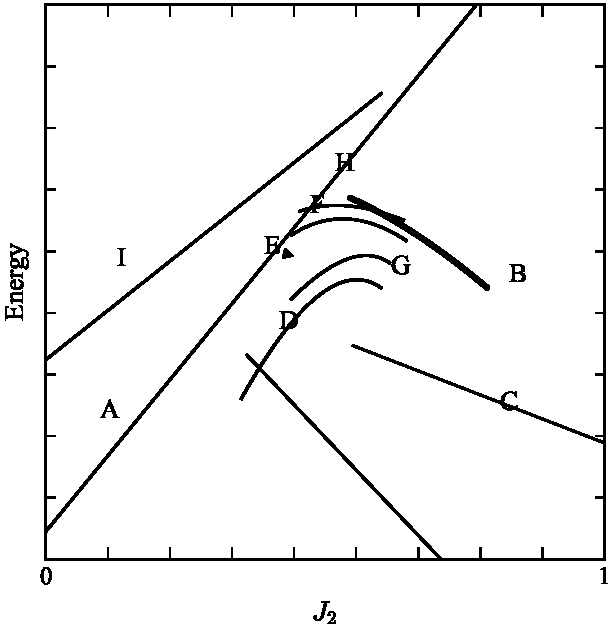
\includegraphics[width=0.72\textwidth]{fig_9.15.pdf}
\caption*{图 9.15\quad $J_1$--$J_2$ 自旋系统中各个相的平均场能量：“A” 标记 $\pi$ 通量态（$SU(2)$ 线性态 SU2Bn0）；“B” 标记式 (9.8.6) 中的 $SU(2)\times SU(2)$ 无能隙态；“C” 标记式 (9.8.7) 中的 $SU(2)\times SU(2)$ 线性态；“D” 标记手征自旋态（一个 $SU(2)$ 有能隙态）；“E” 标记破坏 $90^{\circ}$ 旋转对称性的 $U(1)$ 线性态 (9.8.8)；“F” 标记式 (9.8.9) 中的 $U(1)$ 有能隙态 U1Cn00x；“G” 标记式 (9.6.2) 中的 $Z_2$ 线性态 Z2Azz13；“H” 标记式 (9.6.1) 中的 $Z_2$ 线性态 Z2A0013；“I” 标记均匀 RVB 态（$SU(2)$ 无能隙态 SU2An0）。}
\end{figure}

在大 $N$ 极限下，$SU(2)$ 平均场理论 (9.8.3) 是一个好的近似，因此我们将用平均场理论来计算 $SP(2N)$ 模型的相图。描述平均场基态的平均场拟设通过把平均场能量极小化而求得，结果示于图 9.15。图 9.15 中的每条曲线代表一个局域极小的平均场能量，能量最低的曲线对应于平均场基态。我们发现，每条曲线上不同的拟设都具有同一个 PSG。这在预料之中，因为当我们改变 $J_2$ 时，曲线所描述的平均场能量以解析的方式变化，所以沿同一条曲线从一个点移动到另一个点并不发生量子相变。同一条曲线上的拟设属于同一个相，由同一个 PSG 描述。

然而，如果两条曲线相交，交点就代表一个量子相变，因为基态能量在交点处不是解析的。由于不同的曲线具有不同的 PSG，我们看到量子相变以 PSG 的改变为特征。下面我们将讨论图 9.15 中各平均场相的不同量子序（或 PSG）。

在图 9.15 中，相 A 是式 (9.2.33) 给出的 $\pi$ 通量态（SU2Bn0 $SU(2)$ 线性态）。相 B 是在对角链上带有两个相互独立的均匀 RVB 态的态。它在低能下具有 $SU(2)\times SU(2)$ 规范涨落，将被称为 $SU(2)\times SU(2)$ 无能隙态。其拟设由下式给出：
\begin{equation*}
u_{\pmb{i},\pmb{i}+\pmb{x}+\pmb{y}}=\chi\tau^{3},\qquad
u_{\pmb{i},\pmb{i}+\pmb{x}-\pmb{y}}=\chi\tau^{3},\qquad
a_0^{l}=0.
\tag{9.8.6}
\end{equation*}
相 C 是在对角链上带有两个相互独立的 $\pi$ 通量态的态。它在低能下具有 $SU(2)\times SU(2)$ 规范涨落，将被称为 $SU(2)\times SU(2)$ 线性态。其拟设由下式给出：
\begin{equation*}
u_{\pmb{i},\pmb{i}+\pmb{x}+\pmb{y}}=\chi(\tau^{3}+\tau^{1}),\qquad
u_{\pmb{i},\pmb{i}+\pmb{x}-\pmb{y}}=\chi(\tau^{3}-\tau^{1}),\qquad
a_0^{l}=0
\tag{9.8.7}
\end{equation*}
相 D 是手征自旋态 (9.1.22)。相 E 由拟设
\begin{equation*}
\begin{aligned}
u_{\pmb{i},\pmb{i}+\pmb{x}+\pmb{y}}&=\chi_1\tau^{1}+\chi_2\tau^{2}, &\qquad
u_{\pmb{i},\pmb{i}+\pmb{x}-\pmb{y}}&=\chi_1\tau^{1}-\chi_2\tau^{2}\\
u_{\pmb{i},\pmb{i}+\pmb{y}}&=\eta\tau^{3}, &\qquad
a_0^{l}&=0
\end{aligned}
\tag{9.8.8}
\end{equation*}
描述，它破坏 $90^{\circ}$ 旋转对称性，是一个 $U(1)$ 线性态。相 F 由如下 U1Cn00x 拟设描述：
\begin{equation*}
\begin{aligned}
u_{\pmb{i},\pmb{i}+\pmb{x}}&=\eta\tau^{1}, &\qquad
u_{\pmb{i},\pmb{i}+\pmb{y}}&=\eta\tau^{1}\\
u_{\pmb{i},\pmb{i}+\pmb{x}+\pmb{y}}&=\chi\tau^{3}, &\qquad
u_{\pmb{i},\pmb{i}+\pmb{x}-\pmb{y}}&=\chi\tau^{3}\\
a_0^{3}&=\lambda, &\qquad
a_0^{1,2}&=0.
\end{aligned}
\tag{9.8.9}
\end{equation*}
U1Cn00x 态可以是 $U(1)$ 线性态（若 $a_0^{3}$ 小），也可以是 $U(1)$ 有能隙态（若 $a_0^{3}$ 大）。相 F 的态结果是一个 $U(1)$ 有能隙态。相 G 由式 (9.6.2) 中的 Z2Azz13 拟设描述，是一个 $Z_2$ 线性态。相 H 由式 (9.6.1) 中的 Z2A0013 拟设描述，也是一个 $Z_2$ 线性态。相 I 是均匀 RVB 态（式 (9.2.32) 中的 $SU(2)$ 无能隙态 SU2An0）。

从图 9.15 我们观察到下列各对相之间（在平均场层次上）的连续相变：(A,D)、(A,G)、(B,G)、(C,E) 与 (B,H)。其中三个连续相变 (B,G)、(B,H) 与 (A,G) 不改变任何对称性。我们还注意到，在从相 A 到相 G 的连续相变中，相 A 的 $SU(2)$ 规范结构破缺到 $Z_2$；在 (B,G) 与 (B,H) 这两个相变中，相 B 的 $SU(2)\times SU(2)$ 规范结构破缺到 $Z_2$。

\section{量子序与平均场自旋液体的稳定性}

\begin{keypoints}
\item 许多无能隙平均场自旋液体对量子涨落可以是稳定的。即使存在长程规范相互作用，它们仍可以是稳定的。
\end{keypoints}

我们已经强调了平均场态对平均场涨落的稳定性的重要性。只有稳定的平均场态和边缘的平均场态才有可能描述物理自旋液体。我们在 9.1.5 节和 9.2.2 节中讨论过获得稳定平均场态的途径。这里我们将从量子序及其 PSG 刻画的角度再次讨论平均场态的稳定性。

% 块边界判定：
%   起点——书页 431（p446）顶部为 9.9.1 节标题，起新小节，无前块溢出内容，
%     故本块不设 %JOIN%，亦无需 X-TAIL 区。
%   实际覆盖——9.9.1--9.9.5 节、9.10 节（含 9.10.1、9.10.2）及问题 9.10.1、9.10.2；
%     9.7、9.8 两节与 9.9 节引言在前块 ch9_f（书页 421--430）内。
%   终点——书页 439（p454）以问题 9.10.2 (c) 收束，为第 9 章末页（p455 为第 10 章
%     章首），自然收尾，无需 TAIL。
% 蓝本问题记录：
%   1) 式 (9.10.6) 右端蓝本与原书均印作 $U_{P_x}$，按上下文应为 $U_{P_y}$，已订正并加译注；
%   2) 式 (9.10.6) 引导句蓝本与原书均印作 $G_{P_y}T_{P_y}$，应为 $G_{P_y}P_y$，已按本意
%      译出并加译注；
%   3) 9.10.1 节蓝本 OCR 作 "IGG=\{c^{1(-)^{i}\theta\tau^{3}}\}"，按图片订正为
%      $\{\mathrm{e}^{\mathrm{i}(-)^{\pmb{i}}\theta\tau^{3}}\}$；
%   4) 9.10.2 节 "there will a gapless U(1) gauge boson" 原书漏 "be"，按本意译出；
%   5) 蓝本 9.9.4 节把 Z2Bx2(12)n 误排作 "Z2Bx2(12)n"（与图片一致，无碍）；
%      蓝本 9.9.3 节段首 "wefdw..." 等为文字层 OCR 噪声，未采信。

\subsection{投影对称群——量子相的一个普适性质}

\begin{keypoints}
\item 如果相应的平均场态是稳定的（即没有红外发散），PSG 就是真实量子相的一个普适性质。此时，PSG 描述该量子相中的量子序。
\end{keypoints}

在本节中，我们想证明 PSG 可以成为量子态的一种普适性质，其含义是它对微扰涨落是稳健的。因此，PSG 作为一种普适性质，可以用来刻画一个量子相。任何与 PSG 相联系（或受 PSG 保护）的物理性质也是相的普适性质，可以用于在实验中探测和测量量子序。特别地，PSG 能够保护无能隙规范激发和费米子激发（见 9.10 节）。因此，PSG 的稳定性也蕴含着无能隙规范激发和费米子激发的稳定性。

我们知道，平均场自旋液体态由 $U_{ij}=\langle\psi_{\pmb{i}}\psi_{\pmb{j}}^{\dagger}\rangle$ 刻画。如果在平均场态附近纳入微扰涨落，我们预期 $U_{ij}$ 会获得微扰修正 $\delta U_{ij}$。这里我们想论证：微扰涨落只能以这样的方式改变 $U_{ij}$，使得 $U_{ij}$ 与 $U_{ij}+\delta U_{ij}$ 具有相同的 PSG。

首先，我们想指出以下众所周知的事实。微扰涨落不能改变对称性和规范结构。例如，如果拟设 $U_{ij}$ 与哈密顿量具有某个对称性，那么由微扰涨落生成的 $\delta U_{ij}$ 将具有同样的对称性。类似地，微扰涨落不能生成这样的 $\delta U_{ij}$——比方说，把一个 $U(1)$ 规范结构破缺到 $Z_2$ 规范结构的 $\delta U_{ij}$。

由于规范结构（由 IGG 描述）和对称性群都是 PSG 的一部分，把上述观察推广为“除 PSG 中的 IGG 与对称性群之外，整个 PSG 都不能被微扰涨落改变”是合理的。

事实上，平均场哈密顿量和平均场基态在 PSG 中的变换下是不变的。因此，在围绕一个平均场态的微扰计算中，PSG 中的变换表现得就像普通的对称性变换一样。所以，微扰涨落只能生成在 PSG 的变换下不变的 $\delta U_{ij}$。

由于微扰涨落（按定义）不改变相，$U_{ij}$ 与 $U_{ij}+\delta U_{ij}$ 描述同一个相。换言之，我们可以把 $U_{ij}$ 分成若干类（称为普适类，universality classes），使得每一类中的 $U_{ij}$ 彼此通过微扰涨落相连。每一个普适类描述一个相。我们看到，如果上述论证成立，那么同一普适类中的拟设都享有同一个 PSG。换言之，普适类或者相是由 PSG（或量子序）分类的。

我们想指出，在上面的讨论中我们假定了微扰涨落没有红外发散。红外发散意味着微扰涨落是相关微扰。这种发散的修正可能引起相变，从而使上述论证失效。因此，上述论证和结果只适用于满足下列要求的稳定自旋液体：(i) 所有平均场涨落都没有红外发散；(ii) 平均场涨落在格点尺度上足够弱。

在下文中，我们将讨论几类平均场态的稳定性。要求 (ii) 可以通过大 $N$ 极限和/或（必要时）调整自旋哈密顿量中的短程自旋耦合来满足。这里我们将主要考虑要求 (i)。我们发现，至少在某些大 $N$ 极限下，许多（但并非全部）平均场态确实对应于在低能下稳定的真实量子自旋液体。

迄今为止所研究的所有自旋液体（每个元胞具有奇数个电子）可以分为四类。下面我们将逐一研究每一类。

\subsection{刚性自旋液体}

刚性自旋液体（rigid spin liquid）是自旋子和所有其他激发都完全有能隙的态。规范场的能隙可以由 Chern--Simons 项或 Anderson--Higgs 机制产生。有能隙的规范场只在自旋子之间诱导短程相互作用。由于低能下没有激发，刚性自旋液体是稳定的态。刚性自旋液体由拓扑序刻画，并且具有未禁闭的中性自旋-1/2 激发。刚性自旋液体的低能有效理论是拓扑场论。$Z_2$ 有能隙自旋液体和手征自旋液体是刚性自旋液体的例子。

\subsection{玻色自旋液体}

U1Cn00x 态 (9.8.9) 在式 (9.8.9) 中的 $a_{0}^{3}$ 足够大时，可以是一个 $U(1)$ 有能隙自旋液体。这样的态在平均场层次上具有有能隙的自旋子和无能隙的 $U(1)$ 规范玻色子。我们将称之为玻色自旋液体（Bose spin liquid）。无能隙 $U(1)$ 规范涨落的动力学由如下低能有效理论描述：
\begin{equation*}
\mathcal{L}=\frac{1}{8\pi g^{2}}\left(f_{\mu\nu}\right)^{2}
\end{equation*}
其中 $f_{\mu\nu}$ 是 $U(1)$ 规范场的场强。然而，在 $1+2$ 维中，并且在纳入瞬子效应之后，$U(1)$ 规范涨落将具有红外发散，这导致规范玻色子获得能隙以及自旋子被禁闭（Polyakov, 1977）。因此，平均场 $U(1)$ 有能隙态在 $1+2$ 维中是不稳定的。它们的 PSG 可能并不描述物理自旋液体中任何真实的量子序。\footnote{我们想\emph{提一句}，平均场 $U(1)$ 有能隙态在 $1+3$ 维中是\emph{稳定的}。}

\subsection{费米自旋液体}

费米自旋液体（Fermi spin liquid）由以下两条性质定义。其一，它们具有由自旋-1/2 费米子描述的无能隙激发；其二，这些无能隙激发之间只有短程相互作用。$Z_2$ 线性自旋液体、$Z_2$ 二次方自旋液体和 $Z_2$ 无能隙自旋液体是费米自旋液体的例子。

在 $Z_2$ 线性自旋液体中，自旋子具有无质量的狄拉克色散。这些具有短程相互作用的自旋子在连续极限下由如下有效理论描述（见问题 9.1.4）：
\begin{equation*}
S=\int\mathrm{d}t\,\mathrm{d}^{2}x\,\left[\bar{\psi}\partial_{\mu}\gamma^{\mu}\psi+\left(\bar{\psi}M\psi\right)^{2}\right]
\end{equation*}
在 $2+1$ 维中，$\psi$ 的标度量纲为 $[\psi]=1$，因此作用量是无量纲的。于是，相互作用项 $(\psi)^{4}$ 的标度量纲为 $[\psi^{4}]=4$，比 3 要大。我们看到，无质量狄拉克费米子之间的短程相互作用在 $1+2$ 维中是不相关的。因此，$Z_2$ 线性自旋液体是稳定的态。

现在让我们考虑式 (9.6.10) 中 $Z_2$ 二次方自旋液体 Z2Bx2(12)n 的稳定性。在 $Z_2$ 二次方自旋液体中，自旋子具有无能隙的二次方色散 $\omega\propto k^{2}$。在这种情形下，空间和时间具有不同的标度量纲，分别为 $[x^{-1}]\equiv1$ 与 $[t^{-1}]=2$。从无量纲的连续作用量
\begin{equation*}
S=\int\mathrm{d}t\,\mathrm{d}^{2}x\,\left[\psi^{\dagger}\mathrm{i}\partial_{t}\psi-c\psi^{\dagger}(\partial_{x})^{2}\psi\right]
\end{equation*}
我们看到，自旋子场 $\psi$ 的标度量纲为 $[\psi]=1$，而四费米子相互作用项的量纲为 $[\psi^{4}]=4$。于是，相互作用作用量 $S_{\mathrm{int}}=\int\mathrm{d}t\,\mathrm{d}^{2}x\,g(\psi^{\dagger}\psi)^{2}$ 中的耦合常数 $g$ 的标度量纲为 $[g]=0$，因为 $S_{\mathrm{int}}$ 的标度量纲总是零。因此，与 $Z_2$ 线性自旋液体不同，$Z_2$ 二次方态中无能隙自旋子之间的短程相互作用在 $1+2$ 维中是边缘的。相互作用的高阶效应会使耦合变得相关还是不相关，仍需进一步的研究才能确定。这将决定 $Z_2$ 二次方自旋液体在平均场层次之外的动力学稳定性。

在 $1+2$ 维中，$Z_2$ 无能隙自旋液体与费米液体一样稳定。如果我们假定费米液体在 $1+2$ 维中是稳定的，那么 $Z_2$ 无能隙自旋液体也是稳定的。

\subsection{代数自旋液体}

代数自旋液体（algebraic spin liquid）是具有无能隙激发的态，但其中没有任何一种无能隙激发是由自由的玻色型或费米型准粒子描述的。$U(1)$ 线性自旋液体是代数自旋液体的例子。它们的低能激发由与 $U(1)$ 规范场耦合的无质量狄拉克费米子描述。由于费米子--规范场耦合在微扰论的所有阶都是严格边缘的（Appelquist and Nash, 1990），无能隙激发一直低到零能都具有有限的相互作用。结果，低能下既没有自由的玻色型准粒子（如规范玻色子），也没有自由的费米型准粒子（如自旋子）。这使得关于这些态的稳定性的讨论困难得多。关于代数自旋液体的讨论，感兴趣的读者可参阅 Rantner and Wen (2002) 与 Wen (2002c)。

已经证明，在 $2+1$ 维中，$U(1)$ 线性态在自旋模型的某些平均场涨落微弱的大 $N$ 极限下是稳定的。$U(1)$ 线性态的 PSG 阻止微扰涨落生成破坏稳定性的抵消项（counter term），例如费米子质量项。这保证了 $U(1)$ 线性态的稳定性。因此，至少在大 $N$ 极限下，相应的代数自旋液体作为物理自旋系统的相而存在。

代数自旋液体的存在是一个非常惊人的现象。按照通常的看法，如果玻色子/费米子在低能下相互作用，那么相互作用将为这些低能激发打开一个能隙。这蕴含着：一个系统要么在低能下具有自由的玻色型/费米型激发，要么根本没有低能激发。代数自旋液体的存在表明，这种通常的看法是不正确的。它提出了一个重要问题：是什么保护着无能隙激发（特别是当它们在所有能标上都相互作用时）？无能隙激发的存在应当有一个“理由”或“原理”。在下一节中我们将证明，PSG 阻止规范玻色子和费米子获得质量项。\emph{所以，正是量子序及其相应的 PSG 保护着无能隙激发。}

\section{量子序与无能隙规范玻色子和费米子}

\begin{keypoints}
\item 量子序能够产生并保护无能隙规范玻色子与无能隙费米子，正如对称性破缺能够产生并保护无能隙 Nambu--Goldstone 玻色子一样。
\end{keypoints}

无能隙激发在自然界和凝聚态系统中都非常罕见。因此，如果我们看到一个无能隙激发，我们就会想问它为什么存在。无能隙激发的一种来源是自发对称性破缺，它给出 Nambu--Goldstone 玻色子（Nambu, 1960; Goldstone, 1961）。无能隙激发与自发对称性破缺之间的这种关系非常重要。正是由于这种关系，我们可以在不了解系统细节的情况下，仅从对称性出发得到一个复杂态的低能物理。这一思路使得 Landau 关于相与相变的对称性破缺理论（Ginzburg and Landau, 1950; Landau and Lifschitz, 1958）成为一个研究相的低能性质的极为强有力的理论。然而，自发对称性破缺并不是无能隙激发的唯一来源。量子序及其相应的 PSG 也能产生并保护无能隙激发。令人惊奇的是，量子序产生并保护的是无能隙规范玻色子和无能隙费米子。无能隙费米子甚至可以从纯玻色模型中产生。在本节中，我们想较为详细地讨论量子序（及其 PSG）与无能隙规范/费米子激发之间的关系（Wen, 2002a,c; Wen and Zee, 2002）。

\subsection{投影对称群与无能隙规范玻色子}

\begin{keypoints}
\item （在平均场层次上）无能隙规范玻色子的规范群就是 PSG 的 IGG。
\end{keypoints}

无能隙规范涨落与量子序之间的关系简单而直接。量子有序态中无能隙规范涨落的规范群，就是刻画该量子序的 PSG 中的 IGG。

为了看清量子序及其 PSG 如何产生并保护无能隙规范玻色子，作为一个例子，让我们假定一个量子有序态的 IGG $\mathcal{G}$ 包含一个 $U(1)$ 子群，它由下列常值规范变换构成：
\begin{equation*}
\{W_{\pmb{i}}=\mathrm{e}^{\mathrm{i}\theta\tau^{3}}\,|\,\theta\in[0,2\pi)\}\subset\mathcal{G}
\end{equation*}
接着我们考虑围绕平均场解 $\bar{u}_{ij}$ 的一类涨落，即 $u_{ij}=\bar{u}_{ij}\mathrm{e}^{\mathrm{i}a_{ij}^{3}\tau^{3}}$。由于 $\bar{u}_{ij}$ 在常值规范变换 $\mathrm{e}^{\mathrm{i}\theta\tau^{3}}$ 下不变，一个依赖空间的规范变换 $\mathrm{e}^{\mathrm{i}\theta_{\pmb{i}}\tau^{3}}$ 将把涨落 $a_{ij}^{3}$ 变为 $\tilde{a}_{ij}^{3}=a_{ij}^{3}+\theta_{\pmb{i}}-\theta_{\pmb{j}}$。这意味着 $a_{ij}^{3}$ 与 $\tilde{a}_{ij}^{3}$ 标记同一个物理态，而 $a_{ij}^{3}$ 对应于规范涨落。涨落的能量具有规范不变性，即 $E(\{a_{ij}^{3}\})=E(\{\tilde{a}_{ij}^{3}\})$。由于能量的这种规范不变性，我们看到规范场的质量项 $(a_{ij}^{3})^{2}$ 是不被允许的。因此，由 $a_{ij}^{3}$ 描述的 $U(1)$ 规范涨落将在低能下出现。

如果 $\mathcal{G}$ 的 $U(1)$ 子群由如下依赖空间的规范变换构成：
\begin{equation*}
\{W_{\pmb{i}}=\mathrm{e}^{\mathrm{i}\theta\,\pmb{n}_{\pmb{i}}\cdot\pmb{\tau}}\,|\,\theta\in[0,2\pi),\ |\pmb{n}_{\pmb{i}}|=1\}\subset\mathcal{G},
\end{equation*}
那么我们总可以用一个 $SU(2)$ 规范变换把每个格点上的 $\pmb{n}_{\pmb{i}}$ 转到 $z$ 方向，从而把问题约化为上面讨论过的情形。因此，无论 IGG 中的规范变换是否依赖空间，低能规范涨落的规范群总是由 $\mathcal{G}$ 给出。由于 IGG 的每一个 $U(1)$ 子群都对应于一个无能隙 $U(1)$ 规范玻色子，低能规范玻色子的规范群由 IGG 给出，即使 IGG 是非阿贝尔的。

我们想说明的是，有时低能规范涨落不仅出现在 $\pmb{k}=0$ 附近，还出现在其他一些 $\pmb{k}$ 点附近。在这种情形下，我们将有几个低能规范场，每个 $\pmb{k}$ 点对应一个。9.8 节中讨论的 $SU(2)$ 从属玻色子理论的某些拟设给出了这种现象的例子，它们在低能下具有 $SU(2)\times SU(2)$ 规范结构。我们看到，低能规范结构 $SU(2)\times SU(2)$ 甚至可以比高能规范结构 $SU(2)$ 还要大。即使对于低能规范涨落出现在不同 $\pmb{k}$ 点附近这种复杂情形，IGG 仍然正确地描述相应拟设的低能规范结构。如果 IGG 包含不依赖空间坐标的规范变换，那么这类变换对应于 $\pmb{k}=0$ 附近无能隙规范涨落的规范群。如果 IGG 包含依赖空间坐标的规范变换，那么这些变换对应于非零 $\pmb{k}$ 附近无能隙规范涨落的规范群。例如，若 $\mathrm{IGG}=\{\mathrm{e}^{\mathrm{i}(-)^{\pmb{i}}\theta\tau^{3}}\}$，则在 $\pmb{k}=(\pi,\pi)$ 附近就会出现一个无能隙 $U(1)$ 规范玻色子，由规范场 $(-)^{\pmb{i}}a^{3}(\pmb{x})$ 描述。这样，IGG 为我们提供了对所有低能规范涨落的统一处理，无论它们的晶体动量如何。

在本章中，我们在许多地方使用了 $Z_2$ 自旋液体、$U(1)$ 自旋液体、$SU(2)$ 自旋液体和 $SU(2)\times SU(2)$ 自旋液体这些术语。现在我们可以对这些低能 $Z_2$、$U(1)$、$SU(2)$ 和 $SU(2)\times SU(2)$ 规范群给出精确定义。这些低能规范群就是相应拟设的 IGG。它们与出现在 $SU(2)$、$U(1)$ 或 $Z_2$ 从属玻色子方法中的高能规范群毫无关系。我们还使用过一个平均场态的 $Z_2$ 规范结构、$U(1)$ 规范结构和 $SU(2)$ 规范结构这些术语。它们精确的数学含义同样是相应拟设的 IGG。当我们说一个 $U(1)$ 规范结构被破缺到一个 $Z_2$ 规范结构时，我们的意思是：拟设被改变了，使得它的 IGG 从 $U(1)$ 群变成了 $Z_2$ 群。

\subsection{投影对称群与无能隙费米子}

\begin{keypoints}
\item 有时，一个 PSG 保证无能隙费米子的存在。在这种情形下，PSG 的普适性意味着无能隙费米子的普适性（或稳定性）。
\end{keypoints}

为了演示 PSG 与无能隙费米子之间的直接联系，本节我们将研究一个特定的自旋液体，其量子序由 Z2Azz13 刻画（Wen and Zee, 2002）。Z2Azz13 自旋液体中的自旋子谱由自旋子跳跃哈密顿量
\begin{equation*}
H=\sum_{ij}\psi_{\pmb{i}}^{\dagger}u_{ij}\psi_{\pmb{j}}
\end{equation*}
给出。Z2Azz13 拟设的一个例子由式 (9.6.2) 给出。我们注意到，拟设 $u_{ij}$ 可以看作一个把费米子波函数 $\psi(\pmb{i})$ 映为 $\psi'(\pmb{i})=\sum_{\pmb{j}}u_{ij}\psi(\pmb{j})$ 的算符。这个算符记作 $\hat{H}$，将被称为哈密顿量。$\hat{H}$ 的本征值决定费米子谱。无能隙费米子对应于哈密顿量的零本征值。

Z2Azz13 的 PSG 由
\begin{align*}
G_{x}(\pmb{i}) &= \tau^{0}, & G_{y}(\pmb{i}) &= \tau^{0}\\
G_{P_{x}}(\pmb{i}) &= (-)^{\pmb{i}}\mathrm{i}\tau^{3} & G_{P_{y}}(\pmb{i}) &= (-)^{\pmb{i}}\mathrm{i}\tau^{3}\\
G_{P_{xy}}(\pmb{i}) &= \mathrm{i}\tau^{1} & G_{T}(\pmb{i}) &= \mathrm{i}\tau^{3}\\
G_{0}(\pmb{i}) &= -\tau^{0},\tag{9.10.1}
\end{align*}
生成。复合变换（如 $G_{P_{x}}P_{x}$）也可以看作作用在 $\psi_{\pmb{i}}$ 上的幺正算符。哈密顿量的投影对称性意味着，例如 $G_{P_{x}}P_{x}\hat{H}(G_{P_{x}}P_{x})^{\dagger}=\hat{H}$。

由于 $G_{x}=G_{y}=\tau^{0}$，Z2Azz13 拟设是平移不变的。在动量空间中，哈密顿量具有形式
\begin{equation*}
H(\pmb{k})=\epsilon^{\mu}(\pmb{k})\tau^{\mu}
\end{equation*}
拟设 $u_{ij}$ 在 $G_{T}T$ 下的不变性蕴含 $G_{T}(\pmb{i})u_{ij}G_{T}^{\dagger}(\pmb{j})=-u_{ij}$。用 $\pmb{k}$ 空间的语言表达，我们有
\begin{equation*}
U_{T}H(k_{x},k_{y})U_{T}^{\dagger}=-H(k_{x},k_{y}),\qquad U_{T}=\mathrm{i}\tau^{3}.\tag{9.10.2}
\end{equation*}
其中非平凡的 $G_{T}$ 给出非平凡的 $U_{T}$。式 (9.10.2) 蕴含 $\epsilon^{0,3}(\pmb{k})=0$，以及
\begin{equation*}
H(\pmb{k})=\epsilon^{1}(\pmb{k})\tau^{1}+\epsilon^{2}(\pmb{k})\tau^{2}\tag{9.10.3}
\end{equation*}
拟设在 $G_{P_{xy}}P_{xy}$ 下的不变性给出
\begin{equation*}
U_{P_{xy}}H(k_{x},k_{y})U_{P_{xy}}^{\dagger}=H(k_{y},k_{x}),\qquad U_{P_{xy}}=\mathrm{i}\tau^{1},\tag{9.10.4}
\end{equation*}
其中 $k_{x}$ 与 $k_{y}$ 的交换由 $P_{xy}$ 生成。拟设在 $G_{P_{x}}P_{x}$ 下的不变性导致
\begin{equation*}
U_{P_{x}}H(k_{x},k_{y})U_{P_{x}}^{\dagger}=H(-k_{x}+\pi,\,k_{y}+\pi),\qquad U_{P_{x}}=\mathrm{i}\tau^{3},\tag{9.10.5}
\end{equation*}
\begin{figure}[H]
\centering
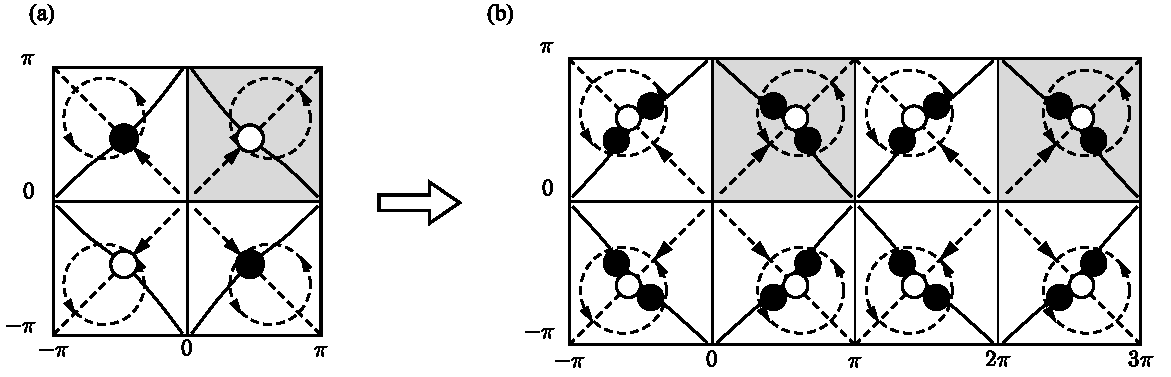
\includegraphics[width=0.72\textwidth]{fig_9.16.pdf}
\caption*{图 9.16\quad $H(\pmb{k})$ 零点的两种图案。$\epsilon^{1}=0$ 线与 $\epsilon^{2}=0$ 线分别用实线和虚线表示。实心圆是缠绕数为 1 的零点，空心圆是缠绕数为 $-1$ 的零点。阴影区域是布里渊区的四分之一。当 $\epsilon^{2}$ 的零线移动而穿过 $\epsilon^{1}$ 的零线时，一个缠绕数为 1 的零点变成一个缠绕数为 $-1$ 的零点加上两个缠绕数为 1 的零点。}
\end{figure}
而拟设在 $G_{P_{y}}P_{y}$ 下的不变性导致
\begin{equation*}
U_{P_{y}}H(k_{x},k_{y})U_{P_{y}}^{\dagger}=H(k_{x}+\pi,\,-k_{y}+\pi),\qquad U_{P_{y}}=\mathrm{i}\tau^{3}.\tag{9.10.6}
\end{equation*}
（译注：原书引导句误印作 $G_{P_{y}}T_{P_{y}}$，式 (9.10.6) 右端误印作 $U_{P_{x}}$，均按上下文订正为 $G_{P_{y}}P_{y}$ 与 $U_{P_{y}}$。）动量平移 $(\pi,\pi)$ 来自 $G_{P_{x}}$ 与 $G_{P_{y}}$ 中的 $(-)^{\pmb{i}}$ 因子。于是，非零的 $\epsilon^{1,2}(\pmb{k})$ 具有下列对称性：
\begin{align*}
\epsilon^{1}(k_{x},k_{y})&=-\epsilon^{1}(\pi-k_{x},\,\pi+k_{y})=-\epsilon^{1}(\pi+k_{x},\,\pi-k_{y})=\epsilon^{1}(k_{y},k_{x})\\
\epsilon^{2}(k_{x},k_{y})&=-\epsilon^{2}(\pi-k_{x},\,\pi+k_{y})=-\epsilon^{2}(\pi+k_{x},\,\pi-k_{y})=-\epsilon^{2}(k_{y},k_{x})\tag{9.10.7}
\end{align*}

事实上，式 (9.10.3) 与式 (9.10.7) 定义了 $\pmb{k}$ 空间中最一般的 Z2Azz13 拟设。

式 (9.10.7) 使我们能够由 $\epsilon^{1,2}(\pmb{k})$ 在布里渊区四分之一区域内的取值确定它们（见图 9.16）。在该四分之一布里渊区内，$\epsilon^{2}(\pmb{k})$ 在 $k_{x}$ 与 $k_{y}$ 互换下是反对称的。因此，当 $k_{x}=k_{y}$ 时 $\epsilon^{2}(\pmb{k})=0$。式 (9.10.7) 还蕴含 $\epsilon^{1}(\pmb{k})$ 在绕 $(0,\pi)$ 或 $(\pi,0)$ 的 $90^{\circ}$ 旋转下变号，即 $\epsilon^{1}(k_{x},k_{y}+\pi)=-\epsilon^{1}(k_{y},-k_{x}+\pi)$。因此，$\epsilon^{1}(\pmb{k})$ 必在 $(0,\pi)$ 与 $(\pi,0)$ 处为零。它在连接 $(0,\pi)$ 与 $(\pi,0)$ 的一条线上也必为零（见图 9.16）。结果，$\epsilon^{1}=0$ 线与 $\epsilon^{2}=0$ 线在四分之一布里渊区内至少相交一次。交点就是哈密顿量 $H(\pmb{k})$ 的零点。我们看到，无能隙自旋子至少出现在布里渊区中四个孤立的 $\pmb{k}$ 点上（见图 9.16）。拟设的 Z2Azz13 对称性直接导致无能隙自旋子。

$H(\pmb{k})$ 的零点的两类典型分布看上去可能就像图 9.16 中那样。我们看到，这些零点具有特殊的图案。为了理解图案中哪些特征是普适的，我们想研究当我们使拟设变形时零点的运动。在这样做之前，我们想指出，$H(\pmb{k})$ 的零点具有一种可以用缠绕数刻画的内部结构。当 $\pmb{k}$ 绕一个零点一周时，二维矢量 $(\epsilon^{1}(\pmb{k}),\epsilon^{2}(\pmb{k}))$ 就围绕 $(0,0)$ 画出一个回路。零点的缠绕数由该回路围绕 $(0,0)$ 缠绕的圈数给出。如果回路围绕 $(0,0)$ 逆时针缠绕，缠绕数为正；如果顺时针缠绕，则为负。典型的零点具有缠绕数 $\pm1$。比如说，一个缠绕数为 2 的零点，在我们微扰哈密顿量之后可以分裂成两个缠绕数为 1 的零点。

对于 Z2Azz13 拟设，$H(\pmb{k})$ 的零点由 $\epsilon^{1}(\pmb{k})$ 与 $\epsilon^{2}(\pmb{k})$ 的零线的交点给出。由于 $\epsilon^{0}(\pmb{k})=\epsilon^{3}(\pmb{k})=0$，所以当我们使拟设变形时，零点不能随意地出现或消失。零点只能成组地产生或湮没，并保持总缠绕数守恒（见图 9.16）。再结合拟设的对称性 (9.10.7)，我们发现下列性质对哈密顿量的任何不改变 PSG 的微小扰动都是稳健的：沿 $((0,0),(\pi,\pi))$ 连线的 $+1$ 与 $-1$ 零点的图案；以及 $(N_{+},N_{-})$，即三角形 $((0,0),(\pi,\pi),(0,\pi))$ \emph{内部} 的 $(+1,-1)$ 零点的数目（不包括边和角上的零点）。我们把这些性质定义为 Z2Azz13 自旋液体的零点图案（pattern of the zero's，POZ）。正如费米面拓扑的改变一样，POZ 的改变将导致基态能量出现奇异性，并标志一个相变。因此，POZ 也是刻画量子序的一个量子数。我们看到，自旋液体中的量子序并不能完全由 PSG 刻画。POZ 提供了一种额外的刻画。PSG 与 POZ 的结合为量子序提供了更完全的刻画。

\subsection*{问题 9.10.1}

考虑式 (9.6.1) 中 Z2A0013 态的一个拟设。你可以假定 $\gamma_{1,2}=\lambda=0$。

(a) 证明：改变 $a_{0}^{1}$ 将引起 POZ 的改变。证明 POZ 的改变会在平均场基态能量中引起奇异性。

(b) 求转变点处低能自旋子的谱。

\subsection*{问题 9.10.2}

(a) 求 Z2A003n PSG 的 $G_{x,y}$、$G_{P_{x},P_{y},P_{xy}}$ 与 $G_{T}$。

(b) 求 Z2A003n 态最一般的平均场哈密顿量 $H(\pmb{k})$。

(c) 证明：Z2A003n 态在 $\pmb{k}=(\pm\frac{\pi}{2},\pm\frac{\pi}{2})$ 处总是具有无能隙自旋子。

% ---------------- 新增术语（ch9_g） ----------------
% | rigid spin liquid | 刚性自旋液体 |
% | Bose spin liquid | 玻色自旋液体 |
% | Fermi spin liquid | 费米自旋液体 |
% | infra-red divergence | 红外发散 |
% | counter term | 抵消项 |
% | lattice scale | 格点尺度 |
% | spinon hopping Hamiltonian | 自旋子跳跃哈密顿量（hopping 系列词沿“跳跃”：跳跃问题/跳跃幅/跳跃算符） |
% | zero-line | 零线 |
% | pattern of the zero's (POZ) | 零点图案（POZ） |
% | winding number of a zero | 零点的缠绕数（缠绕数术语表已收） |
% | momentum shift | 动量平移 |
% | dynamical stability | 动力学稳定性 |
% | spatially-dependent (gauge transformation) | 依赖空间的（规范变换） |
% | constant gauge transformation | 常值规范变换 |

 % 本文件由 scripts/assemble.py 自动装配，勿手改（改 parts/ 后重跑）
% 第10章 弦凝聚——光与费米子的统一

% 第10章 STRING CONDENSATION—AN UNIFICATION OF LIGHT AND FERMIONS

\chapter{弦凝聚——光与费米子的统一}

\begin{keypoints}
\item \textbf{光与费米子是什么？} 光是任意大小的、由凝聚弦构成的网的涨落。费米子是凝聚弦的端点。
\item \textbf{光与费米子从何而来？} 光与费米子来自充满空间的凝聚弦网的集体运动。
\item \textbf{光与费米子为何存在？} 光与费米子之所以存在，是因为我们的真空恰好具有弦网凝聚（string-net condensation）。
\end{keypoints}

在第 9 章中，我们用投影构造在二维自旋系统中构造了许多量子有序态，并引入投影对称群（PSG）来表征和分类这些量子有序态。这些量子有序态不仅包含规范玻色子，而且还包含作为其低能集体激发的费米子。规范玻色子和费米子的演生是一个非常惊人的结果，因为底层的格子模型是一个纯粹的玻色模型。

许多年来，费米子和规范玻色子一直被视为基本的、不可触碰的。当有人提出费米子和规范理论可以从二维自旋液体中演生出来时（Baskaran et al., 1987; Kivelson et al., 1987; Baskaran and Anderson, 1988），这一提议甚至没有引起惊讶，因为它遭遇到的是怀疑与不信。这些怀疑是有根据的。即使到了现在，我们仍不清楚二维自旋液体是否存在。然而，这并不意味着最初的提议是错误的。把这种计算应用到 $SU(N)$ 自旋模型上时（Affleck and Marston, 1988），它的确在三维中给出良好定义的规范玻色子和费米子（见 10.7 节）（Wen, 2002a）。因此，费米子和规范玻色子并非那样基本而不可触碰。它们可以从卑微的玻色模型中的某些量子序演生出来。

然而，导致规范玻色子和费米子演生的投影构造是非常形式化的。似乎一切都依赖于一个非常不合情理的数学技巧——把一个自旋拆成两个非物理的费米子。人们很难对这样一种方法抱有任何信心。由这种方法得到的演生费米子和规范玻色子这一惊人结果，看起来实在难以置信。

本章可以被看作一个建立信心的练习。我们将讨论几个精确可解的自旋模型，它们同样可以用投影构造来求解。我们将证明，对那些模型，投影构造给出的结果与精确结果一致。特别地，正如投影构造所提示的，这些精确可解模型具有演生的费米子和一个规范场。

然而，更重要的是，精确可解模型把费米子和规范场的演生与一种现象——闭合弦网的凝聚——联系在了一起。我们发现，由投影构造得到的量子有序态实际上就是弦网凝聚态。表征由投影构造得到的态中的量子序的 PSG，实际上表征的是不同的弦网凝聚。投影构造与弦网凝聚只是描述同一类量子序的两种不同方式。弦网凝聚为形式化的投影构造提供了一个物理基础。

试图联系投影构造与弦网凝聚，只不过是本章诸讨论的一个形式上的动机。既然费米子和规范玻色子可以从弦网凝聚中演生，我们想为本章的讨论赋予一个更物理的动机。我们想问：弦网凝聚与我们宇宙中光和费米子的存在有没有关系？特别是，我们想就光与费米子提出下面这些问题。光与费米子是什么？光与费米子从何而来？光与费米子为何存在？

目前，对上述基本问题的标准回答似乎是“光是由规范场描写的粒子”以及“费米子是由反对易场描写的粒子”。在这里，我们想论证，对上述问题还存在另一种可能的（而且我相信是更物理的）回答，即：我们的真空充满了任意大小的、由弦状物体构成的网，而这些弦网形成一个量子凝聚态。按照弦网理论，光（以及其他规范玻色子）是凝聚弦网的集体振动，而费米子是弦的端点。我们看到，弦网凝聚为光和费米子提供了一个统一的起源。\footnote{这里，“弦网凝聚”指的是由任意大小的弦状物体构成的网的凝聚。}换句话说，弦网凝聚统一了光与费米子。如果有人说“要有弦网”，那么我们就同时得到了光和费米子。

在为光与费米子的弦网理论提供证据之前，我们想先澄清所谓“光存在”与“费米子存在”是什么意思。我们知道，物理中有一个天然的质量标度——普朗克质量。普朗克质量非常之大，以致我们看到的任何粒子，其质量至少比普朗克质量小 $10^{16}$ 倍。因此，与普朗克质量相比，所有观测到的粒子都可以当作无质量的来处理。当我们问某些粒子为什么存在时，我们的真正意思是：与普朗克质量相比，那些粒子为什么是无质量的（或近乎无质量的）。真正的问题是什么使某些类型的激发（例如光和费米子）成为无质量的（或近乎无质量的）。自然界究竟为什么想要拥有无质量的激发？是谁订购了它们？

其次，我们想澄清所谓“光与费米子的起源”是什么意思。我们知道，一切都必须来自某种东西。所以当我们问“光与费米子从何而来？”时，我们已经假定了存在比光和费米子更简单、更基本的东西。在 10.1 节中，我们将定义局域玻色模型（local bosonic model），它比具有规范场与费米子耦合的模型更简单。我们将把局域玻色模型看作更基本的。这样一种哲学将被称为局域性原理（locality principle）。我们将证明，如果一个局域玻色模型的基态中含有由弦状物体构成的网的凝聚，那么光和费米子就可以从这个模型中演生出来。

费米子的弦网理论解释了为什么我们的宇宙中费米子总是成偶数地出现——因为一条弦（或一个弦网）总有偶数个端点。关于规范玻色子和费米子的弦网理论还有一个实验预言，即所有费米子都必须携带某种规范电荷。乍看之下，这个预言似乎与已知的实验事实——中子不携带任何规范电荷——相矛盾。于是有人可能认为，关于规范玻色子和费米子的弦网理论已经被实验证伪了。这里我们想指出，如果我们假定我们的宇宙中还存在一种新的分立规范场，例如一个 $Z_2$ 规范场，那么关于规范玻色子和费米子的弦网理论仍然可以是正确的。在这种情形下，中子和中微子携带该分立规范场的一个非零电荷。因此，关于规范玻色子和费米子的弦网理论预言，我们的宇宙中存在分立的规范激发（例如规范通量线）。

按照量子序与弦网凝聚的图像，基本粒子（例如光子和电子）可能终究不是基本的。它们可能是普朗克标度以下某个局域玻色系统的集体激发。由于我们无法在接近普朗克标度处做实验，很难判定光子和电子究竟是不是基本粒子。在本章中，我们将通过二维和三维格子上的一些具体的局域玻色模型，证明光与费米子的弦网理论至少是自洽的。这里研究的局域玻色模型，只是长长的局域玻色模型清单中的几个例子，这些模型都包含演生的非禁闭费米子和规范玻色子（Foerster et al., 1980; Kalmeyer and Laughlin, 1987; Wen et al., 1989; Read and Sachdev, 1991; Wen, 1991a; Moessner and Sondhi, 2001; Balents et al., 2002; Ioffe et al., 2002; Motrunich and Senthil, 2002; Sachdev and Park, 2002; Kitaev, 2003; Motrunich, 2003; Wen, 2003c）。这些模型的基态都具有非平凡的拓扑序/量子序。

\begin{smallnote}
我们想指出，尽管有某些相似之处，上述关于规范玻色子和费米子的弦网理论不同于标准的超弦理论。在标准超弦理论中，闭合弦对应于引力子，开弦对应于规范玻色子。费米子来自世界面上的费米型场。超弦理论中所有基本粒子（包括规范玻色子）都对应于小弦的不同振动模式。而在弦网理论中，真空充满了大弦（或大弦构成的网，见图 1.2）。无质量规范玻色子对应于大闭合弦之网的涨落，费米子对应于开弦的端点。弦网理论中没有费米型场。

关于规范涨落的弦网理论与规范理论中的 Wegner--Wilson 圈密切相关（Wegner, 1971; Wilson, 1974; Kogut, 1979）。动力学规范理论与动力学 Wegner--Wilson 圈理论之间的关系由 Gliozzi et al.~(1979) 和 Polyakov (1979) 提出并研究。Savit (1980) 综述了规范理论与延展物体理论之间的各种对偶关系。特别地，人们发现某些统计格点规范模型对偶于某些统计膜模型（Banks et al., 1977）。这种对偶关系与量子模型中规范理论和弦网理论之间的关系直接相连。量子模型中的新特点是，弦的端点有时可以是费米子或任意子（Levin and Wen, 2003）。
\end{smallnote}

这里我们想强调，对于我们宇宙中实际的规范玻色子和费米子而言，弦网理论目前只是一个建议。尽管弦网凝聚能够产生并保护无质量的光子、胶子、夸克以及其他带电轻子，但我们目前还不知道弦网凝聚能否产生中微子——一种手征费米子。我们也不知道弦网凝聚能否产生弱相互作用的 $SU(2)$ 规范场——它与夸克和轻子手征地耦合。弦网凝聚在我们真空中的正确性，取决于上述问题的解决。

另一方面，如果我们只关心凝聚态物理的问题——如何用玻色子制造人工光和人工费米子——那么弦网理论和量子序确实给出了一个答案。要制造人工光和人工费米子，我们只需让某些弦凝聚。

\section{局域玻色模型}

在本章中，我们将只考虑局域玻色模型。我们认为局域玻色模型是基本的，因为它们是真正局域的。我们注意到，费米子模型一般是非局域的，因为不同格点上的费米子算符即使在格点相距很远时也不对易。与此相反，局域玻色模型是局域的，因为相距很远的玻色子算符彼此对易。由于局域玻色模型具有内在的局域性，我们相信自然的基本理论是一个局域玻色模型。为强调这一点，我们将给这一信念起一个名字：局域性原理。

让我们详细定义局域玻色模型。为了定义一个物理系统，我们需要明确（i）一个总希尔伯特空间，（ii）一组局域物理算符的定义，以及（iii）一个哈密顿量。基于这一理解，局域玻色模型定义为满足下列性质的模型：

\begin{enumerate}
\item[(i)] 总希尔伯特空间是有限维局域希尔伯特空间的直积。
\item[(ii)] 局域物理算符是作用在单个局域希尔伯特空间之内的算符，或是这些算符对邻近局域希尔伯特空间的有限乘积。我们也将称这些算符为局域玻色算符，因为相距很远时它们彼此对易。
\item[(iii)] 哈密顿量是局域物理算符之和。
\end{enumerate}

格子上的自旋 $1/2$ 系统是局域玻色模型的一个例子。其局域希尔伯特空间是二维的，包含 $|\uparrow\rangle$ 和 $|\downarrow\rangle$ 态。局域物理算符是 $\sigma_{\pmb{i}}^{a}$、$\sigma_{\pmb{i}}^{a}\sigma_{\pmb{i}+\pmb{x}}^{b}$ 等，其中 $\sigma^{a}$（$a=1,2,3$）是泡利矩阵。

自由的无自旋费米子系统（二维或更高维）不是局域玻色模型，尽管它拥有与自旋 $1/2$ 系统相同的总希尔伯特空间。这是因为不同格点上的费米子算符 $c_i$ 不对易，因而不是局域玻色算符。更重要的是，费米子跳跃算符 $c_i^\dagger c_j$ 在二维及更高维中不能写成局域玻色算符。（不过，由于 Jordan--Wigner 变换，一维费米子跳跃算符 $c_{i+1}^\dagger c_i$ 可以写成局域玻色算符。因此，如果把 $c_i$ 排除在局域物理算符的定义之外，一维费米系统可以是局域玻色模型。）格点规范理论不是局域玻色模型，因为它的总希尔伯特空间不能是局域希尔伯特空间的直积。

\section{由投影构造得到的一个精确可解模型}

在本节中，我们将构造一个精确可解的局域玻色模型。在下一节中，我们将证明该模型包含弦网凝聚和演生的费米子。

\subsection{精确可解模型的构造}

\begin{keypoints}
\item 精确可解模型可以通过寻找彼此对易的算符来构造。
\end{keypoints}

通常，投影构造并不给出精确结果。在本节中，我们将在二维正方格子上构造一个精确可解模型（Kitaev, 2003; Wen, 2003c）。我们的模型具有如下性质：投影构造给出精确的基态以及所有其他精确的激发态。构造的关键一步是找到一组彼此对易的算符。

让我们引入四个马约拉纳费米子（Majorana fermion）算符 $\lambda_{\pmb{i}}^{a}$（$a=x,\bar{x},y,\bar{y}$），满足 $\{\lambda_{a,\pmb{i}},\lambda_{b,\pmb{j}}\}=2\delta_{ab}\delta_{\pmb{i}\pmb{j}}$。我们发现，算符
\begin{equation*}
\hat U_{\pmb{i},\pmb{i}+\hat{\pmb{x}}}=\lambda_{\pmb{i}}^{x}\lambda_{\pmb{i}+\hat{\pmb{x}}}^{\bar{x}},\qquad
\hat U_{\pmb{i},\pmb{i}+\hat{\pmb{y}}}=\lambda_{\pmb{i}}^{y}\lambda_{\pmb{i}+\hat{\pmb{y}}}^{\bar{y}},\qquad
\hat U_{\pmb{i}\pmb{j}}=-\hat U_{\pmb{j}\pmb{i}},
\tag{10.2.1}
\end{equation*}
构成一组彼此对易的算符，即 $[\hat U_{\pmb{i}_1\pmb{i}_2},\hat U_{\pmb{j}_1\pmb{j}_2}]=0$。在得到一组对易算符之后，我们容易看出，作为诸 $\hat U_{\pmb{i}\pmb{j}}$ 的函数，相互作用费米子哈密顿量
\begin{equation*}
H=-\sum_{\pmb{i}}V_{\pmb{i}}\hat F_{\pmb{i}},\qquad
\hat F_{\pmb{i}}=\hat U_{\pmb{i},\pmb{i}_1}\hat U_{\pmb{i}_1,\pmb{i}_2}\hat U_{\pmb{i}_2,\pmb{i}_3}\hat U_{\pmb{i}_3,\pmb{i}},
\tag{10.2.2}
\end{equation*}
与所有 $\hat U_{\pmb{i}\pmb{j}}$ 对易。这里 $\pmb{i}_1=\pmb{i}+\hat{\pmb{x}}$，$\pmb{i}_2=\pmb{i}+\hat{\pmb{x}}+\hat{\pmb{y}}$，而 $\pmb{i}_3=\pmb{i}+\hat{\pmb{y}}$。我们将把 $\hat F_{\pmb{i}}$ 称为 $Z_2$ 通量算符。

为了得到式 (10.2.2) 中的哈密顿量 $H$ 所作用的希尔伯特空间，我们在每个格点上把 $\lambda^{x,\bar{x},y,\bar{y}}$ 组合成两个复费米子算符
\begin{equation*}
2\psi_{1,\pmb{i}}=\lambda_{\pmb{i}}^{x}+\mathrm{i}\lambda_{\pmb{i}}^{\bar{x}},\qquad
2\psi_{2,\pmb{i}}=\lambda_{\pmb{i}}^{y}+\mathrm{i}\lambda_{\pmb{i}}^{\bar{y}}
\tag{10.2.3}
\end{equation*}
可以验证，$\psi_{1,2}$ 满足标准的费米子反对易代数。这两个复费米子算符在每个格点上生成一个四维希尔伯特空间。总希尔伯特空间的维数为 $4^{N_{\text{site}}}$。诸 $\hat U_{\pmb{i}\pmb{j}}$ 与 $H$ 的对易性使我们能够精确地求解这个相互作用费米子系统。

为了得到 $H$ 的精确本征态和精确本征值，令 $|\{s_{ij}\}\rangle$ 为诸 $\hat U_{ij}$ 算符的具有本征值 $s_{ij}$ 的共同本征态。由于 $(\hat U_{ij})^{2}=-1$ 且 $\hat U_{ij}=-\hat U_{ji}$，我们发现 $s_{ij}$ 满足 $s_{ij}=\pm\mathrm{i}$ 且 $s_{ij}=-s_{ji}$。由于 $H$ 是诸 $\hat U_{ij}$ 的函数，我们发现 $|\{s_{ij}\}\rangle$ 也是式 (10.2.2) 的一个能量本征态，其能量为
\begin{equation*}
E=-\sum_{\pmb{i}}V_{\pmb{i}}F_{\pmb{i}},\qquad
F_{\pmb{i}}=s_{\pmb{i},\pmb{i}_1}s_{\pmb{i}_1,\pmb{i}_2}s_{\pmb{i}_2,\pmb{i}_3}s_{\pmb{i}_3,\pmb{i}}
\tag{10.2.4}
\end{equation*}
我们将把 $F_{\pmb{i}}$ 称为穿过方格 $\pmb{i}$ 的 $Z_2$ 通量。当 $V_{\pmb{i}}>0$ 时，基态由 $|\{s_{ij}\}\rangle$ 给出，其中 $s_{\pmb{i},\pmb{i}+\pmb{x}}=s_{\pmb{i},\pmb{i}+\pmb{y}}=\mathrm{i}$。对这样的态，我们有 $F_{\pmb{i}}=1$。为了得到激发态，我们翻转某些 $s_{ij}$ 的符号，使某些 $F_{\pmb{i}}=-1$。

为了考察诸 $|\{s_{ij}\}\rangle$ 是否代表 $H$ 的所有精确本征态，我们需要清点态的数目。设二维正方格子有 $N_{\text{site}}$ 个格点，且两个方向都取周期性边界条件。这时格子有 $2N_{\text{site}}$ 条链。由于 $s_{ij}$ 总共有 $2^{2N_{\text{site}}}$ 种不同的选择（每条链有两种选择），态 $|\{s_{ij}\}\rangle$ 遍尽了希尔伯特空间中全部 $4^{N_{\text{site}}}$ 个态。因此，诸 $\hat U_{\pmb{i}\pmb{j}}$ 的共同本征态不简并，上述方法使我们能够得到 $H$ 的所有本征态和本征值。我们已经精确求解了这个二维相互作用费米子系统！

我们注意到，哈密顿量 $H$ 只能把每个格点上的费米子数改变偶数。因此，$H$ 作用在一个每个格点具有偶数个费米子的子空间之内。我们将称这个子空间为物理希尔伯特空间。物理希尔伯特空间在每个格点上只有两个态。限制在物理空间之内时，$H$ 实际上描写一个自旋 $1/2$ 或硬核玻色子系统。为了得到相应的自旋 $1/2$ 哈密顿量，我们注意到
\begin{equation*}
\sigma_{\pmb{i}}^{x}=\mathrm{i}\lambda_{\pmb{i}}^{y}\lambda_{\pmb{i}}^{x},\qquad
\sigma_{\pmb{i}}^{y}=\mathrm{i}\lambda_{\pmb{i}}^{\bar{x}}\lambda_{\pmb{i}}^{y},\qquad
\sigma_{\pmb{i}}^{z}=\mathrm{i}\lambda_{\pmb{i}}^{x}\lambda_{\pmb{i}}^{\bar{x}}
\tag{10.2.5}
\end{equation*}
作用在物理希尔伯特空间之内，且满足泡利矩阵的代数。因此，我们可以把 $\sigma_{\pmb{i}}^{l}$ 认作自旋算符。利用在物理希尔伯特空间之内
\begin{equation*}
(-)^{\psi^{\dagger}_{1,\pmb{i}}\psi_{1,\pmb{i}}+\psi^{\dagger}_{2,\pmb{i}}\psi_{2,\pmb{i}}}
=\lambda_{\pmb{i}}^{x}\lambda_{\pmb{i}}^{y}\lambda_{\pmb{i}}^{\bar{x}}\lambda_{\pmb{i}}^{\bar{y}}=1
\end{equation*}
这一事实，我们可以证明，费米子哈密顿量 (10.2.2) 变为（见问题 10.2.2）
\begin{equation*}
H_{\text{spin}}=-\sum_{\pmb{i}}V_{\pmb{i}}\hat F_{\pmb{i}},\qquad
\hat F_{\pmb{i}}=\sigma_{\pmb{i}}^{x}\sigma_{\pmb{i}+\hat{\pmb{x}}}^{y}\sigma_{\pmb{i}+\hat{\pmb{x}}+\hat{\pmb{y}}}^{x}\sigma_{\pmb{i}+\hat{\pmb{y}}}^{y}
\tag{10.2.6}
\end{equation*}
在物理希尔伯特空间之内。

物理希尔伯特空间中的所有态（即自旋 $1/2$ 模型中的所有态）都可以从诸 $|\{s_{ij}\}\rangle$ 态投影到物理希尔伯特空间而得到，即 $\mathcal{P}|\{s_{ij}\}\rangle$。投影算符为
\begin{equation*}
\mathcal{P}=\prod_{\pmb{i}}\frac{1+(-)^{\psi^{\dagger}_{1\pmb{i}}\psi_{1\pmb{i}}+\psi^{\dagger}_{2\pmb{i}}\psi_{2\pmb{i}}}}{2}
\end{equation*}
由于 $[\mathcal{P},H]=0$，投影后的态 $\mathcal{P}|\{s_{ij}\}\rangle$（如果非零）仍然是 $H$（或 $H_{\text{spin}}$）的本征态，且具有相同的本征值。经过投影，相互作用费米子模型的精确解导致自旋 $1/2$ 模型的精确解。

我们注意到，对于 $x$ 和 $y$ 两个方向都有周期性边界条件的系统，所有链的乘积
\begin{equation*}
\prod_{\pmb{i}}\,(\mathrm{i}s_{\pmb{i},\pmb{i}+\pmb{x}})(\mathrm{i}s_{\pmb{i},\pmb{i}+\pmb{y}})=(-)^{\hat N_f},
\tag{10.2.7}
\end{equation*}
其中 $\hat N_f=\sum_{\pmb{i}}(\psi^{\dagger}_{1\pmb{i}}\psi_{1\pmb{i}}+\psi^{\dagger}_{2\pmb{i}}\psi_{2\pmb{i}})$ 是总费米子数算符。因此，$|\{s_{ij}\}\rangle$ 的投影非零，仅当
\begin{equation*}
\prod_{\pmb{i}}\,(\mathrm{i}s_{\pmb{i},\pmb{i}+\pmb{x}})(\mathrm{i}s_{\pmb{i},\pmb{i}+\pmb{y}})=1.
\tag{10.2.8}
\end{equation*}

物理态（每个格点具有偶数个费米子）在由
\begin{equation*}
\hat G=\prod_{\pmb{i}}G_{\pmb{i}}^{\;\psi^{\dagger}_{1,\pmb{i}}\psi_{1,\pmb{i}}+\psi^{\dagger}_{2,\pmb{i}}\psi_{2,\pmb{i}}}
\end{equation*}
生成的局域 $Z_2$ 变换下不变，其中 $G_{\pmb{i}}$ 是一个只取 $\pm1$ 两个值的任意函数。我们注意到，$Z_2$ 变换把 $\psi_{I\pmb{i}}$ 变为 $\tilde\psi_{I\pmb{i}}=G_{\pmb{i}}\psi_{I\pmb{i}}$，把 $s_{ij}$ 变为 $\tilde s_{ij}=G_{\pmb{i}}s_{ij}G_{\pmb{j}}$。我们发现，$|\{s_{ij}\}\rangle$ 与 $|\{\tilde s_{ij}\}\rangle$ 在投影后给出同一个物理态（如果它们的投影非零）。于是，$\{s_{ij}\}$ 是自旋 $1/2$ 系统 $H_{\text{spin}}$ 的精确本征态的一个多对一标签。向具有每格点偶数个费米子的物理希尔伯特空间的投影，使我们的理论成为一个 $Z_2$ 规范理论。

\subsection*{问题 10.2.1}

\begin{enumerate}
\item[(a)] 证明式 (10.2.1) 中的诸 $\hat U_{ij}$ 构成一组彼此对易的算符。
\item[(b)] 证明式 (10.2.3) 中的诸 $\psi$ 满足复费米子的标准反对易关系。
\end{enumerate}

\subsection*{问题 10.2.2}

\begin{enumerate}
\item[(a)] 证明 $2\psi_1^\dagger\psi_1-1=\mathrm{i}\lambda^{x}\lambda^{\bar{x}}$ 以及 $2\psi_2^\dagger\psi_2-1=\mathrm{i}\lambda^{y}\lambda^{\bar{y}}$。证明在一个格点上具有偶数个费米子的态是 $\lambda^{x}\lambda^{y}\lambda^{\bar{x}}\lambda^{\bar{y}}$ 的本征值为 $+1$ 的本征态。
\item[(b)] 证明式 (10.2.7)。
\item[(c)] 证明式 (10.2.5) 中的诸 $\sigma^{l}$ 在物理希尔伯特空间内满足泡利矩阵的代数。
\item[(d)] 证明费米子哈密顿量 (10.2.2) 在物理希尔伯特空间内变为自旋哈密顿量 (10.2.6)。
\end{enumerate}

\subsection*{问题 10.2.3}

我们已经看到，把费米子哈密顿量 $H$ 限制在每格点具有偶数个费米子的子空间之内，可以从费米子系统得到一个自旋 $1/2$ 系统。我们注意到，费米子哈密顿量 $H$ 也作用在每格点具有奇数个费米子的子空间之内。试把费米子哈密顿量 $H$ 限制在奇数费米子子空间之内，得到相应的自旋 $1/2$ 系统。

\subsection{精确本征态与拓扑简并的基态}

\begin{keypoints}
\item 基态简并受到 $Z_2$ 规范结构的保护，对任何局域微扰都是稳健的。
\end{keypoints}

上述 $Z_2$ 规范结构使我们能够清点由诸 $|\{s_{ij}\}\rangle$ 态投影得到的物理态的数目。我们再次假定两个方向都有周期性边界条件。注意到常数 $Z_2$ 规范变换 $G_{\pmb{i}}=-1$ 不改变 $s_{ij}$，我们看到，彼此规范等价的互不相同的 $s_{ij}$ 只有 $2^{N_{\text{site}}}/2$ 个。在 $4^{N_{\text{site}}}$ 个 $|\{s_{ij}\}\rangle$ 态中，有 $4^{N_{\text{site}}}/2$ 个满足 $\prod_{\pmb{i}}(\mathrm{i}s_{\pmb{i},\pmb{i}+\pmb{x}})(\mathrm{i}s_{\pmb{i},\pmb{i}+\pmb{y}})=1$（即具有偶数个费米子）。因此，诸 $|\{s_{ij}\}\rangle$ 态的投影至多给我们 $(4^{N_{\text{site}}}/2)\allowbreak/(2^{N_{\text{site}}}/2)\allowbreak=2^{N_{\text{site}}}$ 个物理态。另一方面，所有 $|\{s_{ij}\}\rangle$ 态的投影应当给我们全部 $2^{N_{\text{site}}}$ 个自旋态。因此，不同的 $s_{ij}$ 的 $Z_2$ 规范等价类必须导致独立的物理态，这样投影才能恢复全部 $2^{N_{\text{site}}}$ 个自旋态。$s_{ij}$ 的 $Z_2$ 规范等价类是周期格子上所有物理态的一对一标签。这样，我们能够得到周期格子上 $H_{\text{spin}}$ 的所有本征态和本征值。

我们注意到，$Z_2$ 通量 $F_{\pmb{i}}$ 在 $Z_2$ 规范变换下不变。因此，如果两个位形 $s_{ij}$ 与 $\tilde s_{ij}$ 分别具有不同的 $Z_2$ 通量 $F_{\pmb{i}}$ 与 $\tilde F_{\pmb{i}}$，则 $s_{ij}$ 与 $\tilde s_{ij}$ 必定属于两个不同的 $Z_2$ 规范等价类。两个态 $|s_{ij}\rangle$ 与 $|\tilde s_{ij}\rangle$ 在投影后将导致不同的物理态。这一结果提示，投影后的态（物理态）用 $Z_2$ 通量 $F_{\pmb{i}}$ 来标记更好。结果发现，$F_{\pmb{i}}$ 并不是物理态的一个完美的一对一标签。对于周期性边界条件下的偶 $\times$ 偶格子上的系统，每个 $F_{\pmb{i}}$ 标记 4 个态（即对每一个 $Z_2$ 通量位形 $F_{\pmb{i}}$，有且仅有 4 个物理态给出同一个 $F_{\pmb{i}}$）。具有相同 $F_{\pmb{i}}$ 的 4 个物理态全部具有相同的能量。

为了理解这一四重简并，让我们考虑由某个 $|\{s_{ij}\}\rangle$ 态的投影所给出的一个本征态。其他简并的本征态可以通过施行下列两个变换得到：
\begin{align*}
T_1&:(s_{\pmb{i},\pmb{i}+\pmb{x}},s_{\pmb{i},\pmb{i}+\pmb{y}})\to(s_{\pmb{i},\pmb{i}+\pmb{x}},(-)^{\delta_{iy}}s_{\pmb{i},\pmb{i}+\pmb{y}})\\
T_2&:(s_{\pmb{i},\pmb{i}+\pmb{x}},s_{\pmb{i},\pmb{i}+\pmb{y}})\to((-)^{\delta_{ix}}s_{\pmb{i},\pmb{i}+\pmb{x}},s_{\pmb{i},\pmb{i}+\pmb{y}})
\end{align*}
我们看到，$T_1$ 不改变 $s_{\pmb{i},\pmb{i}+\pmb{x}}$，只在 $i_y=0$ 时翻转 $s_{\pmb{i},\pmb{i}+\pmb{y}}$ 的符号。由构造可知，$T_1$ 与 $T_2$ 不改变 $Z_2$ 通量 $F_{\pmb{i}}$。如果我们把周期格子看作一个环面，那么 $T_1$ 与 $T_2$ 通过环面的两个洞各插入 $\pi$ 通量（见图 9.6）。

在偶 $\times$ 偶格子上，变换 $T_1$ 与 $T_2$ 不改变乘积 $\prod_{\pmb{i}}(\mathrm{i}s_{\pmb{i},\pmb{i}+\pmb{x}})(\mathrm{i}s_{\pmb{i},\pmb{i}+\pmb{y}})$。因此，三个变换 $T_1$、$T_2$ 与 $T_1T_2$ 生成另外三个简并态。我们看到，所有能量本征值都具有四重简并。特别地，自旋 $1/2$ 模型 $H_{\text{spin}}$ 在偶 $\times$ 偶周期格子上具有 4 个简并基态。

在偶 $\times$ 奇格子上，情况稍有不同。$T_2$ 生成的态具有奇数个费米子，不对应于任何物理自旋 $1/2$ 态。因此，我们只能用 $T_1$ 来生成另一个简并态。在偶 $\times$ 奇周期格子上只有两个简并基态（由 $T_1$ 生成）。在奇 $\times$ 奇格子上，也有由 $T_1T_2$ 生成的两个简并基态。

我们注意到，局域地看，$T_1$ 与 $T_2$ 变换与 $Z_2$ 规范变换不可区分。由于物理自旋算符在 $Z_2$ 规范变换下不变，它们在 $T_1$ 与 $T_2$ 变换下也不变。因此，即使我们在精确可解模型 (10.2.6) 上加入任意局域微扰，由 $T_1$ 与 $T_2$ 生成的简并基态仍将保持简并。基态的这一简并是一个稳健的拓扑性质，表明基态中存在非平凡的拓扑序。

\subsection*{问题 10.2.4}

考虑 $L_x\times L_y$ 周期格子上的式 (10.2.6)。我们假定 $V_{\pmb{i}}=V$，只在某一行方格上 $V_{\pmb{i}}=0$。这时可以把该系统看作定义在一个圆柱上，圆柱在 $x$ 方向具有两条圆形边缘。试求系统的基态简并度。这些简并基态可以看作边缘态。证明每个边缘格点有 $\sqrt{2}$ 个边缘态。这意味着边缘激发由一个马约拉纳费米子描写。

\subsection{基态的投影对称群表征}

\begin{keypoints}
\item 式 (10.2.6) 的 $V<0$ 与 $V>0$ 基态具有不同的量子序。
\end{keypoints}

在本节中，我们将假定自旋 $1/2$ 系统 (10.2.6) 中的 $V_{\pmb{i}}$ 是均匀的，即 $V_{\pmb{i}}=V$。我们已经通过把自旋算符写成费米子算符的乘积求解了式 (10.2.6)（见式 (10.2.5)），也就是说，我们用投影构造求解了自旋 $1/2$ 系统。十分有趣的是，对于这个特定的自旋 $1/2$ 系统 (10.2.6)，投影构造竟然给出精确的结果。由于精确基态波函数是由投影构造得到的（即通过投影自由费米子波函数 (9.2.11) 而得到），我们可以用第 9 章发展的 PSG 表征方法来表征基态中的量子序。

第 9 章的讨论限于自旋旋转不变的态。下面，我们将把平均场理论和 PSG 推广到自旋旋转非不变的态。如果我们把 $|\downarrow\rangle$ 态认作零玻色子态 $|0\rangle$，把 $|\uparrow\rangle$ 态认作单玻色子态 $|1\rangle$，那么自旋 $1/2$ 模型 $H_{\text{spin}}$ 也可以看作一个硬核玻色子模型。下面我们将用玻色子图像来描写我们的模型。

为了用投影构造构造量子有序（或纠缠）的多玻色子波函数，我们首先引入“平均场”费米子哈密顿量
\begin{equation*}
H_{\text{mean}}=\sum_{\langle ij\rangle}\left(\psi^{\dagger}_{I,\pmb{i}}u_{ij}^{IJ}\psi_{J,\pmb{j}}+\psi^{\dagger}_{I,\pmb{i}}w_{ij}^{IJ}\psi^{\dagger}_{J,\pmb{j}}+\text{h.c.}\right)
\tag{10.2.9}
\end{equation*}
其中 $I,J=1,2$。我们将用 $u_{ij}$ 和 $w_{ij}$ 表示元素分别为 $u_{ij}^{IJ}$ 和 $w_{ij}^{IJ}$ 的 $2\times2$ 复矩阵。令 $|\Psi^{(u_{ij},w_{ij})}_{\text{mean}}\rangle$ 为上述自由费米子哈密顿量的基态，则下列多体玻色子波函数可以得到：
\begin{equation*}
\Phi^{(u_{ij},w_{ij})}(\pmb{i}_1,\pmb{i}_2...)=\langle0|\prod_{n}b(\pmb{i}_n)|\Psi^{(u_{ij},w_{ij})}_{\text{mean}}\rangle
\tag{10.2.10}
\end{equation*}
其中
\begin{equation*}
b(\pmb{i})=\psi_{1,\pmb{i}}\psi_{2,\pmb{i}}
\tag{10.2.11}
\end{equation*}
我们注意到，物理玻色子波函数 $\Phi^{(u_{ij},w_{ij})}(\{\pmb{i}_n\})$ 在下列 $SU(2)$ 规范变换下不变：
\begin{equation*}
(\psi_{\pmb{i}},u_{ij},w_{ij})\to(G(\pmb{i})\psi_{\pmb{i}},\,G(\pmb{i})u_{ij}G^{\dagger}(\pmb{j}),\,G(\pmb{i})w_{ij}G^{\top}(\pmb{j}))
\end{equation*}
其中 $G(\pmb{i})\in SU(2)$。

玻色子波函数 $\Phi^{(u_{ij},w_{ij})}(\{\pmb{i}_n\})$ 中的量子序可以用 PSG 来表征。PSG 由使拟设 $(u_{ij},w_{ij})$ 不变的对称变换与 $SU(2)$ 规范变换的联合变换构成。

这里我们想指出，诸 $\hat U_{ij}$ 的共同本征态，即 $|\{s_{ij}\}\rangle$，是自由费米子系统
\begin{equation*}
\tilde H_{\text{mean}}=\sum_{\langle ij\rangle}\left(s_{ij}\hat U_{ij}+\text{h.c.}\right)
\tag{10.2.12}
\end{equation*}
的基态。因此，从投影构造的观点看，$\tilde H_{\text{mean}}$ 可以看作“平均场”哈密顿量 $H_{\text{mean}}$。事实上，$\tilde H_{\text{mean}}$ 是 $H_{\text{mean}}$ 的一个特例，其中
\begin{equation*}
-w_{i,i+\hat{\pmb{x}}}=u_{i,i+\hat{\pmb{x}}}=-\mathrm{i}s_{i,i+\hat{\pmb{x}}}(1+\tau^{3}),\qquad
-w_{i,i+\hat{\pmb{y}}}=u_{i,i+\hat{\pmb{y}}}=-\mathrm{i}s_{i,i+\hat{\pmb{y}}}(1-\tau^{3})
\end{equation*}
如果 $s_{ij}$ 与 $(u_{ij},w_{ij})$ 通过上式相联系，则态 $|\{s_{ij}\}\rangle$ 就等于平均场态 $|\Psi^{(u_{ij},w_{ij})}_{\text{mean}}\rangle$。物理自旋波函数由平均场态的投影 $\mathcal{P}|\{s_{ij}\}\rangle$ 得到，这与式 (10.2.10) 等价。

记住，在投影构造中，我们需要选择拟设 $u_{ij}$ 与 $w_{ij}$，使平均能量 $\langle\Psi^{(u_{ij},w_{ij})}_{\text{mean}}|\mathcal{P}H_{\text{spin}}\mathcal{P}|\Psi^{(u_{ij},w_{ij})}_{\text{mean}}\rangle$ 极小。对我们的自旋模型 $H_{\text{spin}}$，这样得到的平庸基态恰好就是精确基态！而且，如果我们选择一个不同的 $s_{ij}$，投影态 $\mathcal{P}|\Psi^{(u_{ij},w_{ij})}_{\text{mean}}\rangle$ 将对应于 $H_{\text{spin}}$ 的一个具有能量 (10.2.4) 的精确本征态。正是在这个意义上，投影构造提供了 $H_{\text{spin}}$ 的一个精确解。

当 $V>0$ 时，我们模型的基态由 $Z_2$ 通量位形 $F_{\pmb{i}}=1$ 给出。为了产生这样的通量，我们可以选择 $s_{\pmb{i},\pmb{i}+\pmb{x}}=s_{\pmb{i},\pmb{i}+\pmb{y}}=\mathrm{i}$。这时，式 (10.2.12) 变为带有
\begin{equation*}
-w_{i,i+\pmb{x}}=u_{i,i+\pmb{x}}=1+\tau^{3},\qquad
-w_{i,i+\pmb{y}}=u_{i,i+\pmb{y}}=1-\tau^{3}.
\end{equation*}
的式 (10.2.9)。为得到上述拟设的 IGG，我们注意到 $u_{ij}$ 在常数规范变换 $G(\pmb{i})=\mathrm{e}^{\mathrm{i}\phi\tau^{z}}$ 下不变。然而，$w_{ij}$ 仅当 $\phi=0,\pi$ 时才不变。于是，IGG $=Z_2$。我们发现低能有效理论是一个 $Z_2$ 规范理论。由于该拟设已经是平移不变的，它在带平凡规范变换 $G_x=G_y=\tau^{0}$ 的 $G_xT_x$ 与 $G_yT_y$ 下不变。上述拟设的 PSG 就是式 (9.4.10) 中的 Z2A PSG。因此，$V>0$ 的基态是一个 Z2A 态。注意，对 Z2A PSG，$G_xT_x$ 与 $G_yT_y$ 满足平移代数 $(G_xT_x)^{-1}(G_yT_y)^{-1}(G_xT_x)(G_yT_y)=1$。

当 $V<0$ 时，基态由位形 $F_{\pmb{i}}=-1$ 给出，它可以由 $s_{\pmb{i},\pmb{i}+\pmb{x}}=(-)^{i_y}s_{\pmb{i},\pmb{i}+\pmb{y}}=\mathrm{i}$ 产生（译注：按本页下方拟设中 $y$ 方向链上的 $(-)^{i_x}$ 因子以及 $F_{\pmb{i}}=-1$ 的要求，此处指数应为 $i_x$，即 $s_{\pmb{i},\pmb{i}+\pmb{y}}=(-)^{i_x}\mathrm{i}$；原文印作 $(-)^{i_y}$）。拟设现在具有形式
\begin{equation*}
-w_{i,i+\pmb{x}}=u_{i,i+\pmb{x}}=1+\tau^{3},\qquad
-w_{i,i+\pmb{y}}=u_{i,i+\pmb{y}}=(-)^{i_x}(1-\tau^{3}).
\end{equation*}
该拟设在平移 $\pmb{i}\to\pmb{i}+\pmb{x}$ 接规范变换 $G_x(\pmb{i})=(-)^{i_y}$ 下不变。它的 PSG 是式 (9.4.11) 中的 Z2B PSG。因此，$V<0$ 的基态是一个 Z2B 态。对 Z2B PSG，$G_xT_x$ 与 $G_yT_y$ 满足磁平移代数 $(G_xT_x)^{-1}(G_yT_y)^{-1}(G_xT_x)(G_yT_y)=-1$。费米子跳跃哈密顿量 $H_{\text{mean}}$ 描写费米子在磁场中的跳跃，每个方格有 $\pi$ 通量。不同的 PSG 告诉我们，$V<0$ 与 $V>0$ 的基态具有不同的量子序。

\section{正方格子上的 $Z_2$ 自旋液体与弦网凝聚}

\begin{keypoints}
\item 弦网凝聚导致演生的 $Z_2$ 规范理论和费米子。
\end{keypoints}

在这一节中，我们将从弦网凝聚的观点（Levin and Wen, 2003）出发，讨论精确可解自旋 $1/2$ 模型 (10.2.6)（Kitaev, 2003; Wen, 2003c）。该模型是最简单的模型之一，它演示了局域玻色模型中弦网凝聚与演生规范玻色子及费米子之间的联系。该模型也可以用从属玻色子方法求解，这使我们能够看到描写量子序的 PSG 如何与弦网凝聚相联系（见 10.4 节）。

\subsection{构造具有闭合弦网凝聚的哈密顿量}

\begin{keypoints}
\item 可以通过让某些弦状物体凝聚来构造具有演生规范场的局域玻色模型。
\end{keypoints}

让我们首先考虑正方格子上一个任意的自旋 $1/2$ 模型。我们想问的第一个问题是：什么样的自旋相互作用能够给出一个低能规范理论？如果我们相信规范理论与弦网理论之间的联系（Banks et al., 1977; Savit, 1980; Wen, 2003a），那么得到低能规范理论的一种途径，是设计一种自旋相互作用，使它允许大闭合弦的强烈涨落，却禁止其他类型的涨落（例如局域自旋翻转、开弦涨落等）。我们希望，大闭合弦的强烈涨落的出现将导致任意大小闭合弦的凝聚，继而给出一个低能规范理论。

\begin{figure}[H]
\centering
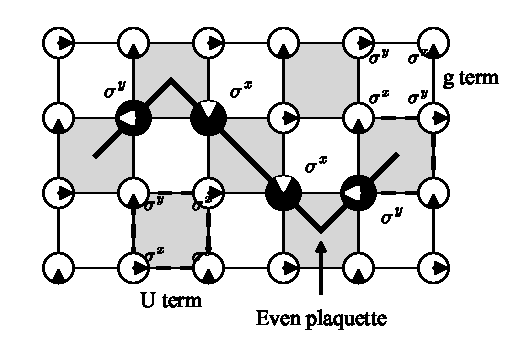
\includegraphics[width=0.72\textwidth]{fig_10.1.pdf}
\caption*{图 10.1\quad $H_J$ 的基态之上的一个开弦激发。}
\end{figure}

让我们从
\begin{equation*}
H_J=-J\sum_{\text{even}}\sigma_{\pmb{i}}^{x}-J\sum_{\text{odd}}\sigma_{\pmb{i}}^{y}
\end{equation*}
出发，其中 $\pmb{i}=(i_x,i_y)$ 标记格点，$\sigma^{x,y,z}$ 是泡利矩阵，而 $\sum_{\text{even}}$（或 $\sum_{\text{odd}}$）对偶格点求和，偶格点满足 $(-)^{\pmb{i}}\equiv(-1)^{i_x+i_y}=1$（或对奇格点求和，奇格点满足 $(-)^{\pmb{i}}=-1$）。$H_J$ 的基态，即 $|0\rangle$，具有这样的性质：偶格点上的自旋指向 $x$ 方向，奇格点上的自旋指向 $y$ 方向（见图 10.1）。这样一个态将被定义为无弦态（no-string state）。

为了产生一个弦激发，我们先画一条连接最近邻偶方格的弦（见图 10.1），然后把弦上的自旋翻转。这样一个弦态由下列弦产生算符（string creation operator，或简称弦算符）产生：
\begin{equation*}
W(C)=-\prod_{C}\sigma_{\pmb{i}}^{a_{\pmb{i}}}
\tag{10.3.1}
\end{equation*}
其中乘积 $\prod_{C}$ 遍及弦上的所有格点，且若 $\pmb{i}$ 为偶则 $a_{\pmb{i}}=y$，若 $\pmb{i}$ 为奇则 $a_{\pmb{i}}=x$。一个一般的弦态具有形式
\begin{equation*}
|C_1C_2...\rangle=W(C_1)W(C_2)...|0\rangle
\end{equation*}
其中 $C_1,C_2,\dots$ 是弦。这样的态将被称为弦网态（string-net state），因为弦可以相交和重叠。产生弦网的算符，即
\begin{equation*}
W(C_{\text{net}})=W(C_1)W(C_2)...
\end{equation*}
% （本块止于书页 452 末行显示公式；其后半句“将被称为弦网算符。”在书页 453 (p468) 顶部，由下一块收尾。）
弦网算符（string-net operator）。只要 $C_i$ 中至少有一个是开弦，态 $|C_1C_2\dots\rangle$ 就是开弦网态。相应的算符 $W(C_{\mathrm{net}})$ 将被称为开弦网算符。若所有 $C_i$ 都是闭合回路，则 $|C_1C_2\dots\rangle$ 就是闭合弦网态，而 $W(C_{\mathrm{net}})$ 是闭合弦网算符。

哈密顿量 $H_J$ 没有弦网凝聚，因为它的基态 $|0\rangle$ 不包含任何弦网，因而 $\langle0|W(C_{\mathrm{net}})|0\rangle=0$。要得到具有闭合弦网凝聚的哈密顿量，我们首先需要找到一个哈密顿量，其基态包含大量任意尺寸的闭合弦网，并且不包含任何开弦（或开弦网）。

让我们先写出一个使闭合弦和闭合弦网不耗费能量、而任何开弦都耗费大量能量的哈密顿量。这样一个哈密顿量可以取如下形式
\begin{equation*}
H_U=-U\sum_{\mathrm{even}}\hat F_{\pmb{i}}
\end{equation*}
其中
\begin{equation*}
\hat F_{\pmb{i}}=\sigma_{\pmb{i}}^{x}\sigma_{\pmb{i}+\pmb{x}}^{y}\sigma_{\pmb{i}+\pmb{x}+\pmb{y}}^{x}\sigma_{\pmb{i}+\pmb{y}}^{y}\tag{10.3.2}
\end{equation*}

我们发现，无弦态 $|0\rangle$ 是 $H_U$ 的基态之一（假定 $U>0$），能量为 $-UN_{\mathrm{site}}$。所有闭合弦态，例如 $W(C_{\mathrm{close}})|0\rangle$，也都是 $H_U$ 的基态，因为 $[H_U,W(C_{\mathrm{close}})]=0$。类似地，$[H_U,W(C_{\mathrm{net}})]=0$ 意味着任何闭合弦态也都是基态。

利用开弦算符 $W(C_{\mathrm{open}})$ 与 $\hat F_{\pmb{i}}$ 之间的对易关系
\begin{align*}
\hat F_{\pmb{i}}W(C_{\mathrm{open}})&=-W(C_{\mathrm{open}})\hat F_{\pmb{i}}, && \text{若 } C_{\mathrm{open}} \text{ 终止于方格 } \pmb{i},\\
\hat F_{\pmb{i}}W(C_{\mathrm{open}})&=+W(C_{\mathrm{open}})\hat F_{\pmb{i}}, && \text{其他情形},
\end{align*}
我们发现，开弦算符在其两个端点处翻转 $\hat F_{\pmb{i}}$ 的符号。开弦态 $W(C_{\mathrm{open}})|0\rangle$ 也是 $\hat F_{\pmb{i}}$ 的本征态，因而是 $H_U$ 的本征态，能量为 $-UN_{\mathrm{site}}+4U$。我们看到，开弦的每个端点耗费能量 $2U$。我们还注意到，闭合弦网的能量不依赖于网中弦的长度。因此，$H_U$ 中的弦没有张力。可以通过在哈密顿量中加入 $H_J$ 来引入弦张力，张力为每格点（或每段）$2J$。我们注意到，任何弦网态 $|C_1C_2\dots\rangle$ 都是 $H_U+H_J$ 的本征态。因此，由 $H_U+H_J$ 描述的弦网不涨落，从而不能凝聚。为使弦发生涨落，我们需要 $g$ 项
\begin{equation*}
H_g=-g\sum_{\pmb{p}}W(C_{\pmb{p}})=-g\sum_{\mathrm{odd}}\hat F_{\pmb{i}}
\end{equation*}
其中 $\pmb{p}$ 标记奇数方格，$C_{\pmb{p}}$ 是围绕方格 $\pmb{p}$ 的闭合弦。当 $H_g$ 作用在弦网态上时，它往弦网中添加一圈弦 $C_{\pmb{p}}$。因此 $g$ 项使弦发生涨落。我们的自旋 1/2 模型的总哈密顿量为
\begin{equation*}
H=H_U+H_J+H_g
\end{equation*}

当 $U\gg g\gg J$ 时，闭合弦几乎没有张力，$H_g$ 诱发的涨落不受张力的限制。因此，基态包含闭合弦的强烈涨落。换言之，基态被任意尺寸的闭合弦所充满。若 $U\gg g$，则闭合弦断开成开弦要耗费过多能量。因此，当 $U\gg g\gg J$ 时，我们自旋 1/2 模型的基态包含闭合弦凝聚（或者更确切地说，闭合弦网凝聚）。下面我们将研究这样一种弦网凝聚态的物理性质。

\subsection*{问题 10.3.1}

(a) 证明各 $\hat F_{\pmb{i}}$ 在 $x$ 与 $y$ 两个方向均为周期性边界条件的格子上满足
\begin{equation*}
\prod_{\pmb{i}}\hat F_{\pmb{i}}=1\tag{10.3.3}
\end{equation*}
式 (10.3.2) 中的负号使上述简单结果成为可能。

(b) 在两方向均为周期性边界条件的偶 $\times$ 偶格子上，证明各 $\hat F_{\pmb{i}}$ 满足更强的条件
\begin{equation*}
\prod_{\pmb{i}=\mathrm{even}}\hat F_{\pmb{i}}=1\tag{10.3.4}
\end{equation*}

\subsection{弦网凝聚与低能有效理论}

\begin{keypoints}\item 弦网凝聚给出规范激发。\end{keypoints}

让我们先讨论 $U\gg g>0$、$J=0$ 的弦网凝聚相。当 $J=0$ 时，模型 $H_U+H_g$ 成为上一节讨论过的模型 (10.2.6)，其中在偶数格点 $V_{\pmb{i}}=U$，在奇数格点 $V_{\pmb{i}}=g$。该模型是精确可解的，因为 $[\hat F_{\pmb{i}},\hat F_{\pmb{j}}]=0$（Kitaev, 2003）。$H_U+H_g$ 的本征态可以由 $\hat F_{\pmb{i}}$ 的共同本征态得到，即 $|\{F_{\pmb{i}}\}\rangle$，其中 $F_{\pmb{i}}$ 是 $\hat F_{\pmb{i}}$ 的本征值。由于 $\hat F_{\pmb{i}}^{2}=1$，$\hat F_{\pmb{i}}$ 的本征值就是 $F_{\pmb{i}}=\pm1$。$|\{F_{\pmb{i}}\}\rangle$ 的能量为 $E=-U\sum_{\pmb{i}=\mathrm{even}}F_{\pmb{i}}-g\sum_{\pmb{i}=\mathrm{odd}}F_{\pmb{i}}$。

注意到，对于尺寸为 $L_x\times L_y$ 的偶 $\times$ 偶周期格子上的有限系统，各 $\hat F_{\pmb{i}}$ 满足约束 $\prod_{\pmb{i}=\mathrm{even}}\hat F_{\pmb{i}}=1$ 与 $\prod_{\pmb{i}=\mathrm{odd}}\hat F_{\pmb{i}}=1$。因此，各 $F_{\pmb{i}}$ 并不独立，只能标记 $2^{L_xL_y}/4$ 种不同的组态。然而，我们自旋 1/2 模型的希尔伯特空间包含 $2^{L_xL_y}$ 个态。为了复现这 $2^{L_xL_y}$ 个态，$\hat F_{\pmb{i}}$ 的共同本征态必定是四重简并的。这与上一节得到的结果一致。

在 $U\gg g$ 的极限下，所有包含开弦的态都将具有量级为 $U$ 的能量。低能态只包含闭合弦网，并且满足
\begin{equation*}
F_{\pmb{i}}\big|_{\pmb{i}=\mathrm{even}}=1
\end{equation*}
不同的低能态由奇数方格上的 $F_{\pmb{i}}$ 标记，即 $F_{\pmb{i}}\big|_{\pmb{i}=\mathrm{odd}}=\pm1$。特别地，基态由下式给出
\begin{equation*}
F_{\pmb{i}}\big|_{\pmb{i}=\mathrm{odd}}=1.
\end{equation*}

这样的基态具有闭合弦凝聚。这是因为所有闭合弦算符 $W(C_{\mathrm{close}})$ 都与 $H_U+H_g$ 对易。于是，$H_U+H_g$ 的基态 $|\Psi_0\rangle$ 是 $W(C_{\mathrm{close}})$ 的本征态，并且满足
\begin{equation*}
\langle\Psi_0|W(C_{\mathrm{close}})|\Psi_0\rangle=1.
\end{equation*}

上式还意味着基态 $|\Psi_0\rangle$ 是各种闭合弦网组态的等权叠加。

基态之上的低能激发可以通过把某些奇数方格上的 $F_{\pmb{i}}$ 从 1 翻转到 $-1$ 得到。若把奇数方格上的 $F_{\pmb{i}}$ 视为 Z$_2$ 规范理论中的通量，我们发现模型的低能部分与 Z$_2$ 格点规范理论完全相同——至少对无限系统如此。这表明我们模型的低能有效理论是 Z$_2$ 格点规范理论。

然而，有人可能会反对这一结果，指出我们模型的低能部分也同样与在每个奇数方格上放一个自旋的伊辛模型相同，因此低能有效理论应当是伊辛模型。我们想指出，尽管对无限系统而言我们模型的低能部分与伊辛模型相同，但对有限系统而言，我们模型的低能部分不同于伊辛模型。例如，在具有周期性边界条件的有限偶 $\times$ 偶格子上，我们模型的基态有四重简并（Kitaev, 2003; Wen, 2003c）。伊辛模型没有这种简并，而 Z$_2$ 规范理论有这种简并。此外，我们的模型包含一种可以认定为 Z$_2$ 电荷（Z$_2$ charge）的激发。因此，我们模型的低能有效理论是 Z$_2$ 格点规范理论，而不是伊辛模型。奇数方格上 $F_{\pmb{i}}=-1$ 的激发可以视为 Z$_2$ 格点规范理论中的 Z$_2$ 涡旋激发。

为理解 Z$_2$ 电荷激发，我们注意到，在弦凝聚态中，弦不耗费能量，并且是不可观测的。把闭合弦算符作用到基态上，得到的仍是基态自身。由于弦不可观测，一段开弦的行为就像两个独立的粒子。开弦的每个端点对应偶数方格上的一个粒子。产生这样一个粒子所需的能量为 $U$ 的量级。现在，让我们考虑这样一个粒子围绕四个最近邻偶数方格的跳跃（见图 10.2）。每一步跳跃由一小段弦算符产生。我们看到，四个跳跃振幅的乘积由这四个偶数方格正中央那个奇数方格上 $\hat F_{\pmb{i}}$ 的本征值给出。这正是电荷与通量之间的关系。因此，若把奇数方格上的 $F_{\pmb{i}}$ 认定为 Z$_2$ 通量，则偶数方格上弦的端点就对应于 Z$_2$ 电荷。由于闭合弦凝聚，开弦的端点不被禁闭，彼此之间只有短程相互作用。因此，Z$_2$ 电荷的行为就像不挂着弦的点粒子。

\begin{figure}[H]
\centering
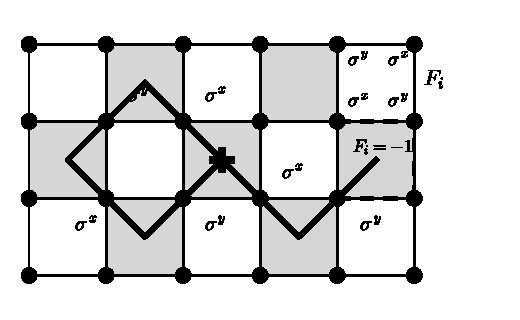
\includegraphics[width=0.72\textwidth]{fig_10.2.pdf}
\caption*{图 10.2\quad Z$_2$ 电荷围绕四个最近邻偶数方格的一次跳跃。}
\end{figure}

\subsection{三种类型的弦与演生费米子}

\begin{keypoints}\item 弦的端点是规范荷。某些弦的端点还可以是费米子。\end{keypoints}

下面我们将研究几种不同类型的弦。为避免混淆，我们把上面讨论的弦称为 T1 弦。T1 弦连接偶数方格（见图 10.3(a)）。

正如 Z$_2$ 电荷一样，一对 Z$_2$ 涡旋也由开弦算符产生。由于 Z$_2$ 涡旋对应于奇数方格上被翻转的 $\hat F_{\pmb{i}}$，产生 Z$_2$ 涡旋的开弦算符同样由式 (10.3.1) 给出，只是现在乘积遍及一条连接\emph{奇数}方格的弦。我们把这样的弦称为 T2 弦。

我们想指出，T2 弦的参考态（即无弦态）不同于 T1 弦的参考态。无 T2 弦态由 $|\tilde{0}\rangle$ 给出，其自旋在偶数格点指向 $y$ 方向、在奇数格点指向 $x$ 方向。由于 T1 弦与 T2 弦有不同的参考态，我们不能同时拥有 T1 弦和 T2 弦的稀薄气体。容易验证，T2 弦算符也与 $H_J+H_g$ 对易。因此，基态 $|\Psi_0\rangle$ 除了 T1 闭合弦的凝聚之外，还有 T2 闭合弦的凝聚。

\begin{figure}[H]
\centering
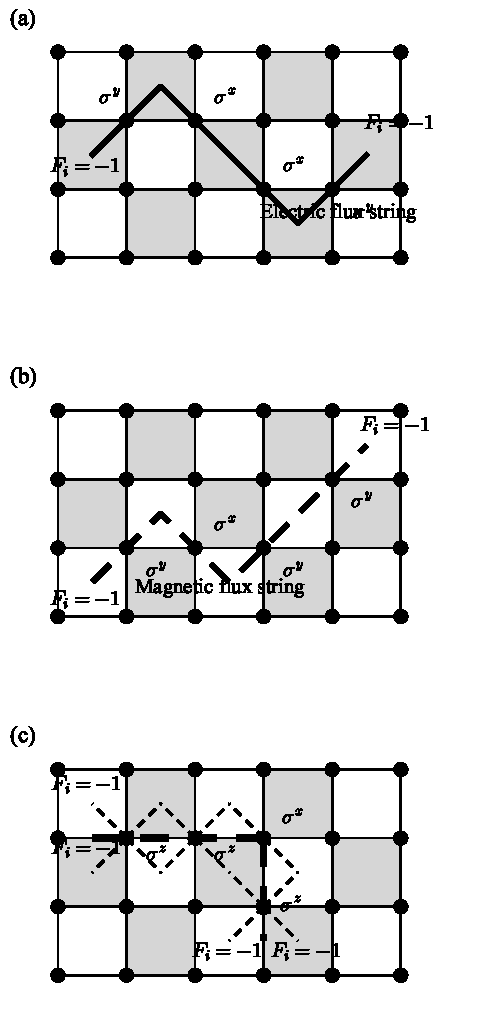
\includegraphics[width=0.72\textwidth]{fig_10.3.pdf}
\caption*{图 10.3\quad 三种类型的弦：(a) T1 弦；(b) T2 弦；(c) T3 弦。}
\end{figure}

Z$_2$ 涡旋的跳跃由一段短的 T2 开弦诱导。由于 T2 开弦算符彼此都对易，Z$_2$ 涡旋的行为像玻色子。类似地，Z$_2$ 电荷的行为也像玻色子。然而，T1 开弦算符与 T2 开弦算符不对易。结果是，T1 弦的端点与 T2 弦的端点具有非平凡的互统计。鉴于我们已经证明，让 Z$_2$ 电荷绕 Z$_2$ 涡旋运动一周会产生相位 $\pi$，Z$_2$ 电荷与 Z$_2$ 涡旋具有半子型（semionic）互统计。

T3 弦定义为 T1 弦与 T2 弦的束缚态（见图 10.3(c)）。T3 弦算符由一个 T1 弦算符与一个 T2 弦算符的乘积给出，具有如下形式
\begin{equation*}
W(C)=\prod_n\sigma_{\pmb{i}_n}^{l_n}
\end{equation*}
其中 $C$ 是一条连接相邻链（link）中点的弦，$\pmb{i}_n$ 是弦上的格点。这里，若弦在格点 $\pmb{i}_n$ 处不拐弯，则 $l_n=z$；若弦在格点 $\pmb{i}_n$ 处拐弯，则 $l_n=x$ 或 $y$；若拐弯构成右上角或左下角，则 $l_n=x$；若拐弯构成右下角或左上角，则 $l_n=y$（见图 10.3(c)）。基态也有 T3 闭合弦的凝聚。T3 弦的端点是由一条链两侧两个方格上的一个 Z$_2$ 电荷与一个 Z$_2$ 涡旋形成的束缚态（即链两侧的 $F_{\pmb{i}}=-1$）。这样的束缚态是费米子（见 7.1.2 节与图 7.8）。所以费米子生活在链上。有趣的是，我们模型中的弦网凝聚直接导致 Z$_2$ 规范结构和三种新类型的准粒子，即 Z$_2$ 电荷、Z$_2$ 涡旋和费米子。费米子作为开 T3 弦的端点，从我们这个纯玻色模型中演生出来！

由于 T1 弦的端点是 Z$_2$ 电荷，T1 弦可以视为 Z$_2$“电”通量的弦。类似地，T2 弦可以视为 Z$_2$“磁”通量的弦。

\section{用投影对称群对不同的弦网凝聚分类}

\subsection{四类弦网凝聚}

\begin{keypoints}\item 不同的弦网凝聚给出不同的量子有序相。\end{keypoints}

我们已经看到，当 $U>0$、$g>0$、$J=0$ 时，我们模型 $H_g+H_U+H_J$ 的基态由下式给出
\begin{equation*}
F_{\pmb{i}}\big|_{\pmb{i}=\mathrm{even}}=1,\qquad F_{\pmb{i}}\big|_{\pmb{i}=\mathrm{odd}}=1.
\end{equation*}
我们将把这样的相称为 Z$_2$ 相，以强调其低能 Z$_2$ 规范结构。在 Z$_2$ 相中，T1 弦算符 $W_1(C_1)$ 与 T2 弦算符 $W_2(C_2)$ 有如下期望值：
\begin{equation*}
\langle W_1(C_1)\rangle=1,\qquad \langle W_2(C_2)\rangle=1
\end{equation*}

当 $U>0$、$g<0$、$J=0$ 时，基态由下式给出
\begin{equation*}
F_{\pmb{i}}\big|_{\pmb{i}=\mathrm{even}}=1,\qquad F_{\pmb{i}}\big|_{\pmb{i}=\mathrm{odd}}=-1.
\end{equation*}
我们看到每个奇数方格都有 $\pi$ 通量。我们将把这样的相称为 Z$_2$ 通量相。T1 弦算符与 T2 弦算符有如下期望值：
\begin{equation*}
\langle W_1(C_1)\rangle=(-)^{N_{\mathrm{odd}}},\qquad \langle W_2(C_2)\rangle=1
\end{equation*}
其中 $N_{\mathrm{odd}}$ 是被 T1 弦 $C_1$ 包围的奇数方格的数目。

当 $U<0$、$g>0$、$J=0$ 时，基态由下式给出
\begin{equation*}
F_{\pmb{i}}\big|_{\pmb{i}=\mathrm{even}}=-1,\qquad F_{\pmb{i}}\big|_{\pmb{i}=\mathrm{odd}}=1.
\end{equation*}
每个偶数方格上有一个 Z$_2$ 电荷。我们将把这样的相称为 Z$_2$ 电荷相。T1 弦算符与 T2 弦算符有如下期望值：
\begin{equation*}
\langle W_1(C_1)\rangle=1,\qquad \langle W_2(C_2)\rangle=(-)^{N_{\mathrm{even}}}
\end{equation*}
其中 $N_{\mathrm{even}}$ 是被 T2 弦 $C_2$ 包围的偶数方格的数目。注意，Z$_2$ 通量相与 Z$_2$ 电荷相仅相差一个格子平移，本质上是同一个相。

当 $U<0$、$g<0$、$J=0$ 时，基态变为
\begin{equation*}
F_{\pmb{i}}\big|_{\pmb{i}=\mathrm{even}}=-1,\qquad F_{\pmb{i}}\big|_{\pmb{i}=\mathrm{odd}}=-1.
\end{equation*}
每个偶数方格上有一个 Z$_2$ 电荷，且每个奇数方格有 $\pi$ 通量。我们将把这样的相称为 Z$_2$ 通量--电荷相。T1 弦算符与 T2 弦算符有如下期望值：
\begin{equation*}
\langle W_1(C_1)\rangle=(-)^{N_{\mathrm{odd}}},\qquad \langle W_2(C_2)\rangle=(-)^{N_{\mathrm{even}}}
\end{equation*}

当 $U=g=0$、$J\neq0$ 时，模型同样精确可解。基态是一个简单的自旋极化态（见图 10.1）。

从 $H_U+H_g+H_J$ 模型的这些精确可解极限出发，我们提出一幅相图，草图示于图 10.4。该相图包含四个不同的弦网凝聚相和一个无弦凝聚的相。所有的相都有相同的对称性，仅凭它们不同的量子序相互区分。

\subsection{投影对称群与凝聚弦的端点}

\begin{keypoints}\item PSG 所描述的投影对称性，正是凝聚弦端点有效理论的对称性。\end{keypoints}

从各不相同的 $\langle W_1(C_1)\rangle$ 与 $\langle W_2(C_2)\rangle$ 我们看到，前四个相具有不同的弦网凝聚。然而，它们都有相同的对称性。这就引出一个问题：在没有对称性破缺的情况下，我们怎么知道上述四个相的确是不同的相？我们怎么知道不可能在不经历相变的情况下把一个弦网凝聚态变成另一个弦网凝聚态？

\begin{figure}[H]
\centering
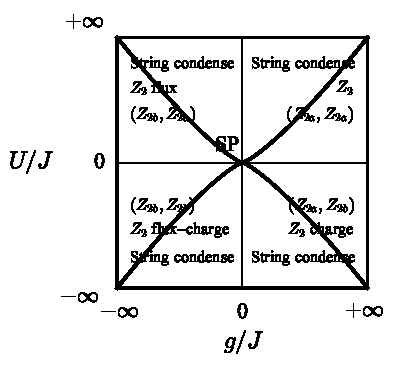
\includegraphics[width=0.72\textwidth]{fig_10.4.pdf}
\caption*{图 10.4\quad $H=H_U+H_g+H_J$ 模型的建议相图。这里假定 $J$ 为正。四个弦网凝聚相由一对 PSG（$PSG_{\mathrm{charge}}$，$PSG_{\mathrm{vortex}}$）表征。SP 标记自旋极化相。}
\end{figure}

下面我们将证明，不同的弦网凝聚可以用不同的 PSG 来描述（正如不同的对称性破缺序可以用基态的不同对称群来描述）。在第 9 章中，不同的量子序是通过它们不同的 PSG 引入的（Wen, 2002b,c）。那里证明了 PSG 是量子相的普适性质，只有相变才能改变 PSG。因此，不同的弦网凝聚态由不同的 PSG 表征，这一事实表明这些不同的弦网凝聚态属于不同的量子相。

弦网凝聚与 PSG 之间的联系也使我们能够把弦网凝聚与第 9 章引入的量子序联系起来。事实上，第 9 章讨论的投影构造可以视为构造弦网凝聚态的一种方法。

为看清 PSG 与弦网凝聚之间的联系，我们注意到，当闭合弦网凝聚时，开弦的端点表现得像独立的粒子。让我们考虑描述 T1 弦两个端点的双粒子态 $|\pmb{p}_1\pmb{p}_2\rangle$。注意，T1 弦的端点（因而 Z$_2$ 电荷）只生活在偶数方格上。因此，$\pmb{p}_1$ 与 $\pmb{p}_2$ 只标记偶数方格。对于我们的模型 $H_U+H_g$，$|\pmb{p}_1\pmb{p}_2\rangle$ 是能量本征态，而且 Z$_2$ 电荷不跳跃。这里我们想往哈密顿量中加入一项
\begin{equation*}
H_t=t\sum_{\pmb{i}}(\sigma_{\pmb{i}}^{x}+\sigma_{\pmb{i}}^{y})+t'\sum_{\pmb{i}}\sigma_{\pmb{i}}^{z}
\end{equation*}
$t$ 项 $t\sum_{\pmb{i}}(\sigma_{\pmb{i}}^{x}+\sigma_{\pmb{i}}^{y})$ 使 Z$_2$ 电荷在偶数方格之间跳跃，跳跃幅为 $t$ 的量级。两个 Z$_2$ 电荷的动力学由双粒子希尔伯特空间中的如下有效哈密顿量描述：
\begin{equation*}
H=H(\pmb{p}_1)+H(\pmb{p}_2)
\end{equation*}
其中 $H(\pmb{p}_1)$ 描述第一个粒子 $\pmb{p}_1$ 的跳跃，$H(\pmb{p}_2)$ 描述第二个粒子 $\pmb{p}_2$ 的跳跃。现在我们可以定义弦网凝聚态的 PSG 了：PSG 就是跳跃哈密顿量 $H(\pmb{p})$ 的对称群。

由于底层模型 $H_U+H_g+H_t$ 具有平移对称性，我们可能天真地预期 Z$_2$ 电荷的跳跃哈密顿量 $H(\pmb{p})$ 在 $\pmb{x}+\pmb{y}$ 与 $\pmb{x}-\pmb{y}$ 方向也具有平移对称性：
\begin{align*}
H(\pmb{p})&=T_{xy}^{\dagger}H(\pmb{p})T_{xy}, & T_{xy}|\pmb{p}\rangle&=|\pmb{p}+\pmb{x}+\pmb{y}\rangle\\
H(\pmb{p})&=T_{x\bar{y}}^{\dagger}H(\pmb{p})T_{x\bar{y}}, & T_{x\bar{y}}|\pmb{p}\rangle&=|\pmb{p}+\pmb{x}-\pmb{y}\rangle\tag{10.4.1}
\end{align*}
如果上式成立，则意味着 PSG 与平移对称群相同。

结果表明，式 (10.4.1) 过强。即使 $H(\pmb{p})$ 不满足式 (10.4.1)，底层自旋模型仍然可以具有平移对称性。然而，$H(\pmb{p})$ 可能的对称群（即各个 PSG）受到底层自旋模型平移对称性的很强约束。下面我们将解释，为什么 PSG 可以不同于物理自旋模型的对称群，以及为与底层自旋模型的平移对称性相一致，PSG 必须满足什么条件。

我们注意到，弦总有两个端点。因此，一个物理态总是拥有偶数个 Z$_2$ 电荷。平移作用在双粒子态上为
\begin{align*}
T_{xy}^{(2)}|\pmb{p}_1,\pmb{p}_2\rangle&=|\pmb{p}_1+\pmb{x}+\pmb{y},\ \pmb{p}_2+\pmb{x}+\pmb{y}\rangle\\
T_{x\bar{y}}^{(2)}|\pmb{p}_1,\pmb{p}_2\rangle&=|\pmb{p}_1+\pmb{x}-\pmb{y},\ \pmb{p}_2+\pmb{x}-\pmb{y}\rangle
\end{align*}
这里 $T_{xy}^{(2)}$ 与 $T_{x\bar{y}}^{(2)}$ 满足平移代数
\begin{equation*}
T_{xy}^{(2)}T_{x\bar{y}}^{(2)}=T_{x\bar{y}}^{(2)}T_{xy}^{(2)}\tag{10.4.2}
\end{equation*}

我们注意到，$T_{xy}^{(2)}$ 与 $T_{x\bar{y}}^{(2)}$ 是单粒子态上平移算符的直积。因此，在某种意义上，单粒子平移是双粒子平移的平方根。双粒子平移代数对单粒子平移代数施加了很强的约束。

单粒子平移最一般的形式由 $T_{xy}G_{xy}$ 与 $T_{x\bar{y}}G_{x\bar{y}}$ 给出，其中算符 $T_{xy,x\bar{y}}$ 与 $G_{xy,x\bar{y}}$ 的作用定义为
\begin{align*}
T_{xy}|\pmb{p}\rangle&=|\pmb{p}+\pmb{x}+\pmb{y}\rangle, & T_{x\bar{y}}|\pmb{p}\rangle&=|\pmb{p}+\pmb{x}-\pmb{y}\rangle,\\
G_{xy}|\pmb{p}\rangle&=\mathrm{e}^{\phi_{xy}(\pmb{p})}|\pmb{p}\rangle, & G_{x\bar{y}}|\pmb{p}\rangle&=\mathrm{e}^{\phi_{x\bar{y}}(\pmb{p})}|\pmb{p}\rangle.
\end{align*}
为了使直积 $T_{xy}^{(2)}=T_{xy}G_{xy}\otimes T_{xy}G_{xy}$ 与 $T_{x\bar{y}}^{(2)}=T_{x\bar{y}}G_{x\bar{y}}\otimes T_{x\bar{y}}G_{x\bar{y}}$ 复现平移代数 (10.4.2)，我们只要求 $T_{xy}G_{xy}$ 与 $T_{x\bar{y}}G_{x\bar{y}}$ 满足
\begin{equation*}
T_{xy}G_{xy}T_{x\bar{y}}G_{x\bar{y}}=T_{x\bar{y}}G_{x\bar{y}}T_{xy}G_{xy}\tag{10.4.3}
\end{equation*}
或
\begin{equation*}
T_{xy}G_{xy}T_{x\bar{y}}G_{x\bar{y}}=-T_{x\bar{y}}G_{x\bar{y}}T_{xy}G_{xy}\tag{10.4.4}
\end{equation*}

算符 $T_{xy}G_{xy}$ 与 $T_{x\bar{y}}G_{x\bar{y}}$ 生成一个群，这个群正是 PSG。两个不同的代数 (10.4.3) 与 (10.4.4) 生成两个不同的 PSG，二者都与作用在双粒子态上的平移群相一致。我们把由式 (10.4.3) 生成的 PSG 称为 Z2a PSG，把由式 (10.4.4) 生成的 PSG 称为 Z2b PSG。

让我们回顾一下 PSG 的一般定义。PSG 是一个群，它是对称群（SG）的扩张，即 PSG 包含一个正规子群（称为不变规范群或 IGG），使得
\begin{equation*}
PSG/IGG=SG
\end{equation*}

在我们的情形中，SG 是平移群 $SG=\{1,T_{xy}^{(2)},T_{x\bar{y}}^{(2)},\dots\}$。IGG 由单粒子态上满足 $G_0\otimes G_0=1$ 的变换 $G_0$ 构成。我们发现 IGG 由下式生成：
\begin{equation*}
G_0|\pmb{p}\rangle=-|\pmb{p}\rangle
\end{equation*}

单粒子态上的这三个变换 $G_0$、$T_{xy}G_{xy}$ 与 $T_{x\bar{y}}G_{x\bar{y}}$ 生成 Z2a 或 Z2b PSG。

我们现在看到，底层平移对称性并不要求单粒子跳跃哈密顿量 $H(\pmb{p})$ 具有平移对称性，只要求 $H(\pmb{p})$ 在 Z2a PSG 或 Z2b PSG 下不变。当 $H(\pmb{p})$ 在 Z2a PSG 下不变时，跳跃哈密顿量具有通常的平移对称性。当 $H(\pmb{p})$ 在 Z2b PSG 下不变时，跳跃哈密顿量具有磁平移对称性，描述磁场中每个奇数方格带 $\pi$ 通量的跳跃。

\subsection{投影对称群对不同的弦网凝聚的分类}

\begin{keypoints}\item 不同的弦网凝聚有不同的 PSG。由于 PSG 是量子相的普适性质，我们发现不同的弦网凝聚对应于不同的相。\end{keypoints}

在了解了弦端点的跳跃哈密顿量可能具有的 PSG 之后，我们现在可以计算实际的 PSG 了。让我们考虑模型 $H_U+H_g+H_t$ 的两个基态：一个具有 $F_{\pmb{i}}\big|_{\pmb{i}=\mathrm{odd}}=1$（对应 $g>0$），另一个具有 $F_{\pmb{i}}\big|_{\pmb{i}=\mathrm{odd}}=-1$（对应 $g<0$）。两个基态在 $\pmb{x}+\pmb{y}$ 与 $\pmb{x}-\pmb{y}$ 方向都有相同的平移对称性。然而，相应的单粒子跳跃哈密顿量 $H(\pmb{p})$ 却有不同的对称性。对于 $F_{\pmb{i}}\big|_{\pmb{i}=\mathrm{odd}}=1$ 的态，奇数方格没有通量，$H(\pmb{p})$ 具有通常的平移对称性，在 Z2a PSG 下不变。对于 $F_{\pmb{i}}\big|_{\pmb{i}=\mathrm{odd}}=-1$ 的态（译注：原文此处印作“$F_{\pmb{i}}|_{\pmb{i}=\mathrm{odd}}=1$”，按上下文应为 $-1$），奇数方格有 $\pi$ 通量，$H(\pmb{p})$ 具有磁平移对称性，其 PSG 为 Z2b PSG。因此，$F_{\pmb{i}}\big|_{\pmb{i}=\mathrm{odd}}=1$ 的态与 $F_{\pmb{i}}\big|_{\pmb{i}=\mathrm{odd}}=-1$ 的态尽管对称性相同，却有不同的序。两个态中不同的量子序可以用它们不同的 PSG 来表征。

如 10.4.1 小节所述，上述两个态有不同的弦网凝聚。对 $\hat F_{\pmb{i}}\big|_{\pmb{i}=\mathrm{odd}}=1$ 的态，T1 闭合弦算符的平均值为 $\langle W(C)\rangle=1$；而对 $\hat F_{\pmb{i}}\big|_{\pmb{i}=\mathrm{odd}}=-1$ 的态，T1 闭合弦算符的平均值为 $\langle W(C)\rangle=(-)^{N_{\mathrm{odd}}(C)}$，其中 $N_{\mathrm{odd}}(C)$ 是被 T1 闭合弦 $C$ 包围的奇数方格的数目。因此，我们也可以说，不同的弦网凝聚可以用不同的 PSG 来表征。

在上面的讨论中，我们只在一些特定的精确可解模型中表明了 PSG 可以表征不同的弦网凝聚态。事实上，在一般模型中，不同的 PSG 确实表征不同的量子相。这是因为，正如 9.9.1 小节所证明的，PSG 是相的普适性质（Wen, 2002c）。弦网凝聚态的 PSG 对物理模型的任何不改变模型对称性的局域微扰都是稳健的。

上述讨论同样适用于 Z$_2$ 涡旋与 T2 弦。因此，我们模型中的量子序由一对 PSG（$PSG_{\mathrm{charge}}$，$PSG_{\mathrm{vortex}}$）描述，一个对应 Z$_2$ 电荷，一个对应 Z$_2$ 涡旋。PSG 对（$PSG_{\mathrm{charge}}$，$PSG_{\mathrm{vortex}}$）使我们能够区分模型 $H=H_U+H_g+H_t$ 的四个不同的弦网凝聚态（见图 10.5）。

\subsection{T3 弦端点的投影对称群}

\begin{keypoints}\item 对于具有几种不同类型弦凝聚的态，不同凝聚弦的端点可以有不同的投影对称性和不同的 PSG。\end{keypoints}

\begin{figure}[H]
\centering
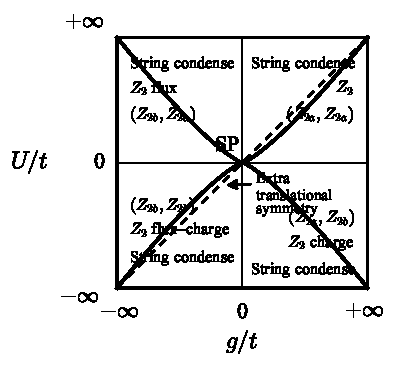
\includegraphics[width=0.72\textwidth]{fig_10.5.pdf}
\caption*{图 10.5\quad $H=H_U+H_g+H_t$ 模型的建议相图。这里假定 $t=t'$ 为正。四个弦网凝聚相由 PSG 对（$PSG_{\mathrm{charge}}$，$PSG_{\mathrm{vortex}}$）表征。SP 标记均匀自旋极化相。所有的相都有相同的对称性，并且没有任何相变改变对称性。}
\end{figure}

\begin{keypoints}\item 9.4.2 小节引入的 PSG 对应于 T3 弦的 PSG。\end{keypoints}

在本小节中，我们将假设模型中 $U=g=V$：
\begin{equation*}
H_U+H_g+H_t=H_t-V\sum_{\pmb{i}}\hat F_{\pmb{i}}\tag{10.4.5}
\end{equation*}

新模型具有由 $\pmb{i}\to\pmb{i}+\pmb{x}$ 与 $\pmb{i}\to\pmb{i}+\pmb{y}$ 生成的更大的平移对称性（见图 10.5）。注意到，当 $H_t=0$ 时（译注：原文此处印作“$H_l=0$”，应为 $H_t$），新模型与 10.2.1 小节研究过的自旋哈密顿量 (10.2.6) 相同。凝聚的 T1 弦与 T2 弦的 PSG 已在上一小节研究过，这里我们想讨论 T3 弦的 PSG。由于 T3 弦的端点生活在链上，相应的单粒子跳跃哈密顿量 $H_f(\pmb{l})$ 描述费米子在链之间的跳跃。显然，$H_f(\pmb{l})$ 的对称群（即 PSG）可以不同于 $H(\pmb{p})$ 的对称群。

让我们把费米子跳跃 $\pmb{l}\to\pmb{l}+\pmb{x}$ 定义为两步跳跃 $\pmb{l}\to\pmb{l}+\frac{\pmb{x}}{2}-\frac{\pmb{y}}{2}\to\pmb{l}+\pmb{x}$ 的组合（见图 10.6）。跳跃 $\pmb{l}\to\pmb{l}+\frac{\pmb{x}}{2}-\frac{\pmb{y}}{2}$ 由 $\sigma_{\pmb{l}+\frac{\pmb{x}}{2}}^{x}$ 产生，跳跃 $\pmb{l}+\frac{\pmb{x}}{2}-\frac{\pmb{y}}{2}\to\pmb{l}+\pmb{x}$ 由 $\sigma_{\pmb{l}+\frac{\pmb{x}}{2}}^{y}$ 产生。因此，跳跃 $\pmb{l}\to\pmb{l}+\pmb{x}$ 由 $\sigma_{\pmb{l}+\frac{\pmb{x}}{2}}^{y}\sigma_{\pmb{l}+\frac{\pmb{x}}{2}}^{x}$ 产生。类似地，我们把费米子跳跃 $\pmb{l}\to\pmb{l}+\pmb{y}$ 定义为两步跳跃 $\pmb{l}\to\pmb{l}+\frac{\pmb{x}}{2}+\frac{\pmb{y}}{2}\to\pmb{l}+\pmb{y}$，它由 $\sigma_{\pmb{l}+\frac{\pmb{x}}{2}+\pmb{y}}^{x}\sigma_{\pmb{l}+\frac{\pmb{x}}{2}}^{y}$ 产生。
\begin{figure}[H]
\centering
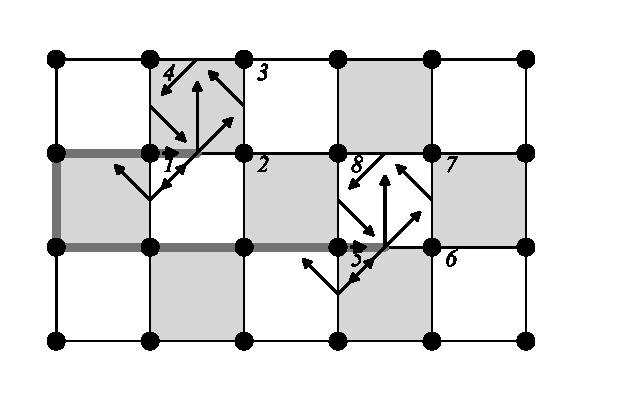
\includegraphics[width=0.72\textwidth]{fig_10.6.pdf}
\caption*{图 10.6\quad 费米子绕一个方格和绕一个格点的跳跃。}
\end{figure}
在这样的定义下，费米子绕方格 $\pmb{l}\to\pmb{l}+\pmb{x}\to\pmb{l}+\pmb{x}+\pmb{y}\to\pmb{l}+\pmb{y}\to\pmb{l}$ 跳跃一周由下式产生（见图 10.6）：$(\sigma_1^{y}\sigma_4^{x})(\sigma_4^{x}\sigma_4^{y})(\sigma_3^{x}\sigma_2^{y})(\sigma_1^{y}\sigma_1^{x})=\sigma_4^{y}\sigma_3^{x}\sigma_2^{y}\sigma_1^{x}=\hat F_1$，或者 $(\sigma_5^{z})(\sigma_5^{y}\sigma_8^{x})(\sigma^{z})(\sigma_7^{x}\sigma_6^{y})=-\sigma_5^{x}\sigma_8^{y}\sigma_7^{x}\sigma_6^{y}=-\hat F_5$。基态具有 $F_{\pmb{i}}=\mathrm{sgn}(V)$。然而，由于 T3 弦终止在链 $5\to6$ 上，我们有 $-\hat F_5=\hat F_{\pmb{i}}=\mathrm{sgn}(V)$；另一方面，我们有 $\hat F_1=\hat F_{\pmb{i}}=\mathrm{sgn}(V)$。因此，费米子绕 1234 与 5678 两个方格跳跃的总振幅由式 (10.4.5) 中 $V$ 的符号给出。当 $\mathrm{sgn}(V)=1$ 时，费米子看不到通量；而当 $\mathrm{sgn}(V)=-1$ 时，费米子看到每个方格有 $\pi$ 通量。结果是，$H_f(\pmb{l})$ 平移对称性的生成元 $(T_xG_x,\,T_yG_y)$ 满足磁平移代数（见式 (7.2.3)）
\begin{equation*}
(T_yG_y)^{-1}(T_xG_x)^{-1}T_yG_yT_xG_x=\mathrm{sgn}(V).\tag{10.4.6}
\end{equation*}

除了在 $(T_xG_x,\,T_yG_y)$ 下不变之外，$H_f(\pmb{l})$ 在 $G_0$ 下也不变：
\begin{equation*}
G_0|\pmb{l}\rangle=-|\pmb{l}\rangle
\end{equation*}
于是，$(G_0,\,T_xG_x,\,T_yG_y)$ 生成 $H_f(\pmb{l})$ 的对称群——费米子 PSG。

当 $\mathrm{sgn}(V)=1$ 时，$T_xG_x$ 与 $T_yG_y$ 满足平移代数，相应的费米子 PSG 是 Z2A PSG。当 $\mathrm{sgn}(V)=-1$ 时，$T_xG_x$ 与 $T_yG_y$ 满足每个方格带 $\pi$ 通量的磁平移代数，相应的费米子 PSG 是 Z2B PSG。我们看到，基态的量子序也可以用费米子 PSG 来表征。$V<0$ 基态的量子序由 Z2A PSG 表征，而 $V>0$ 基态的量子序由 Z2B PSG 表征。

在 10.2 节中，自旋 1/2 模型 (10.4.5)（取 $t=t'=0$）曾通过把自旋拆成两个费米子、用从属玻色子方法求解。那里证明了，$V>0$ 与 $V<0$ 两种态的费米子跳跃哈密顿量具有不同的对称性，或者说在不同的 PSG 下不变。不同的 PSG 意味着 $V>0$ 与 $V<0$ 基态中不同的量子序。10.2 节中针对 $V>0$ 与 $V<0$ 相得到的 PSG 与
这里我们想指出，9.4 节中引入的 PSG 都是费米子 PSG。它们只是可用于刻画量子序的众多不同种类的 PSG 中的一种。一般地说，一个量子有序态可以包含几种不同类型弦的凝聚，每一类凝聚弦的端点都将拥有各自的 PSG。找出所有类型的凝聚弦及其 PSG，将使我们能够对量子序作出更完备的刻画。

\section{立方格子上的演生费米子与弦网凝聚}

\begin{keypoints}
\item 三维模型中的演生费米子，无法用把通量附着到玻色子上的方式来理解。要理解三维中的演生费米子，确实需要弦网理论。
\end{keypoints}

在 $2+1$ 维中，把 $\pi$ 通量束缚到一个单位电荷上（或者把一个 $Z_2$ 涡旋束缚到一个 $Z_2$ 电荷上），便可以得到一个费米子。在我们的自旋 $1/2$ 模型 $H_U+H_g$ 中，我们正是这样得到费米子的。由于 $Z_2$ 涡旋与 $Z_2$ 电荷都以开弦端点的形式出现，费米子也以弦端点的形式出现。我们看到，对于 $(2+1)$ 维玻色模型中的演生费米子，我们有两套理论：演生费米子既可以视为电荷与通量的束缚态，也可以视为弦的端点。然而，在 $3+1$ 维中，我们不能通过附着 $\pi$ 通量把玻色子变成费米子。于是人们或许会问：费米子能否从 $(3+1)$ 维的局域玻色模型中演生出来？本节我们将研究立方格子上一个精确可解的自旋 $3/2$ 模型。我们将研究这样一个模型中的弦网凝聚态，并证明费米子仍然可以作为弦的端点出现。事实上，关于演生费米子的弦网理论在任意维数下都成立。

\subsection{立方格子上的精确可解自旋 $3/2$ 模型}

为了在三维立方格子上构造一个精确可解模型，我们先引入算符 $\gamma_{\pmb{i}}^{ab}$，$a,b=x,\bar{x},y,\bar{y},z,\bar{z}$，它们作用在每个格点的局域希尔伯特空间之内。在一个格点上，$\gamma^{ab}$ 满足以下代数（格点指标 $\pmb{i}$ 已略去）：
\begin{align*}
\gamma^{ab}&=-\gamma^{ba}=(\gamma^{ab})^{\dagger}, & (\gamma^{ab})^{2}&=1, \tag{10.5.1}\\
[\gamma^{ab},\gamma^{cd}]&=0, & \gamma^{ab}\gamma^{bc}&=\mathrm{i}\gamma^{ac}, \qquad \text{若 } a,b,c,d \text{ 互不相同}
\end{align*}

为了证明这个代数是自洽的，令 $\lambda^{a}$ 为一个由 $a=x,\bar{x},y,\bar{y},z,\bar{z}$ 标记的马约拉纳费米子算符。从马约拉纳费米子的代数 $\{\lambda^{a},\lambda^{b}\}=2\delta_{ab}$ 出发可以证明，
\begin{equation*}
\gamma^{ab}=\frac{\mathrm{i}}{2}\left(\lambda_{\pmb{i}}^{a}\lambda_{\pmb{i}}^{b}-\lambda_{\pmb{i}}^{b}\lambda_{\pmb{i}}^{a}\right)
\end{equation*}
满足上述代数。

上述代数有一个四维表示。我们首先注意到，$\gamma^{az}\equiv\gamma^{a}$（$a=x,\bar{x},y,\bar{y}$）满足狄拉克代数
\begin{equation*}
\{\gamma^{a},\gamma^{b}\}=2\delta_{ab}, \qquad a,b=x,\bar{x},y,\bar{y}. \tag{10.5.2}
\end{equation*}
因此，我们可以用四个 $4\times4$ 狄拉克矩阵把它们表示为
\begin{align*}
\gamma^{xz}=\gamma^{x}=\sigma^{x}\otimes\sigma^{x}, & & \gamma^{\bar{x}z}=\gamma^{\bar{x}}=\sigma^{y}\otimes\sigma^{x}, &\\
\gamma^{yz}=\gamma^{y}=\sigma^{z}\otimes\sigma^{x}, & & \gamma^{\bar{y}z}=\gamma^{\bar{y}}=\sigma^{0}\otimes\sigma^{y}. & \tag{10.5.3}
\end{align*}
我们还可以定义
\begin{equation*}
\gamma^{5}=\gamma^{x}\gamma^{\bar{x}}\gamma^{y}\gamma^{\bar{y}}=-\sigma^{0}\otimes\sigma^{z}
\end{equation*}
它与 $\gamma^{a}$ 反对易，即 $\{\gamma^{a},\gamma^{5}\}=0$。由于 $\gamma^{z\bar{z}}$ 与 $\gamma^{az}\equiv\gamma^{a}$（$a=x,\bar{x},y,\bar{y}$）反对易，我们可以把 $\gamma^{5}$ 认同为 $\gamma^{z\bar{z}}$。利用代数 (10.5.1)，可以把其余的 $\gamma^{ab}$ 表示为
\begin{equation*}
\gamma^{a\bar{z}}=\mathrm{i}\gamma^{a}\gamma^{5}, \qquad a=x,\bar{x},y,\bar{y}
\end{equation*}
这样，我们就把全部 $\gamma^{ab}$（$a,b=x,\bar{x},y,\bar{y},z,\bar{z}$）用狄拉克矩阵 $\gamma^{x,\bar{x},y,\bar{y}}$ 表示了出来。可以证明，这样定义的 $\gamma^{ab}$ 满足代数 (10.5.1)。

由于 $\gamma^{ab}$ 是四维的，我们可以说它们作用在自旋 $3/2$ 态上。借助 $\gamma_{\pmb{i}}^{ab}$，我们可以在立方格子上写出一个精确可解的自旋 $3/2$ 模型如下：
\begin{align*}
H_{3D}&\\
&=g\sum_{\pmb{i}}\Big(\gamma_{\pmb{i}}^{yx}\gamma_{\pmb{i}+\pmb{x}}^{\bar{x}y}\gamma_{\pmb{i}+\pmb{x}+\pmb{y}}^{\bar{y}\bar{x}}\gamma_{\pmb{i}+\pmb{y}}^{x\bar{y}}+\gamma_{\pmb{i}}^{zy}\gamma_{\pmb{i}+\pmb{y}}^{\bar{y}z}\gamma_{\pmb{i}+\pmb{y}+\pmb{z}}^{\bar{z}\bar{y}}\gamma_{\pmb{i}+\pmb{z}}^{y\bar{z}}+\gamma_{\pmb{i}}^{xz}\gamma_{\pmb{i}+\pmb{z}}^{\bar{z}x}\gamma_{\pmb{i}+\pmb{z}+\pmb{x}}^{\bar{x}\bar{z}}\gamma_{\pmb{i}+\pmb{x}}^{z\bar{y}}\Big)\\
&=-g\sum_{\pmb{p}}\hat F_{\pmb{p}} \tag{10.5.4}
\end{align*}
其中 $\pmb{p}$ 标记立方格子中的方格，而视方格 $\pmb{p}$ 的取向，$\hat F_{\pmb{p}}$ 等于 $-\gamma_{\pmb{i}}^{yx}\allowbreak\gamma_{\pmb{i}+\pmb{x}}^{\bar{x}y}\allowbreak\gamma_{\pmb{i}+\pmb{x}+\pmb{y}}^{\bar{y}\bar{x}}\allowbreak\gamma_{\pmb{i}+\pmb{y}}^{x\bar{y}}$、$-\gamma_{\pmb{i}}^{zy}\allowbreak\gamma_{\pmb{i}+\pmb{y}}^{\bar{y}z}\allowbreak\gamma_{\pmb{i}+\pmb{y}+\pmb{z}}^{\bar{z}\bar{y}}\allowbreak\gamma_{\pmb{i}+\pmb{z}}^{y\bar{z}}$ 或 $-\gamma_{\pmb{i}}^{xz}\allowbreak\gamma_{\pmb{i}+\pmb{z}}^{\bar{z}x}\allowbreak\gamma_{\pmb{i}+\pmb{z}+\pmb{x}}^{\bar{x}\bar{z}}\allowbreak\gamma_{\pmb{i}+\pmb{x}}^{z\bar{y}}$。

注意到
\begin{equation*}
[\hat F_{\pmb{p}},\hat F_{\pmb{p}}']=0, \qquad (\hat F_{\pmb{p}})^{2}=1,
\end{equation*}
就容易求出 $H_{3D}$ 的本征值。设 $|\{F_{\pmb{p}}\},\alpha\rangle$ 是 $\hat F_{\pmb{p}}$ 的共同本征态，即 $\hat F_{\pmb{p}}|\{F_{\pmb{p}}\},\alpha\rangle=F_{\pmb{p}}|\{F_{\pmb{p}}\},\alpha\rangle$，其中 $\alpha$ 标记可能的简并。那么 $|\{F_{\pmb{p}}\},\alpha\rangle$ 也是能量本征态，能量为 $-g\sum_{\pmb{p}}F_{\pmb{p}}$。由于 $F_{\pmb{p}}=\pm1$，在周期性格子上基态能量为 $E_0=-3|g|N_{\text{site}}$，其中 $N_{\text{site}}$ 是格点数目。激发态可以通过翻转某些 $F_{\pmb{p}}$ 的符号得到，其能量为 $E_0$ 加上 $2|g|$ 的整数倍。

有一个微妙之处：诸 $F_{\pmb{p}}$ 并不全部独立。若 $S$ 是一个单胞立方体的表面，则有算符恒等式
\begin{equation*}
\prod_{\pmb{p}\in S}\hat F_{\pmb{p}}=1
\end{equation*}
由此可知，对所有立方体都有 $\prod_{\pmb{p}\in S}F_{\pmb{p}}=1$。如果我们把 $F_{\pmb{p}}$ 看作穿过方格 $\pmb{p}$ 的 $Z_2$ 通量，那么上述约束就意味着通量守恒。这意味着我们模型的能谱与立方格子上一个 $Z_2$ 规范理论的能谱相同。基态可以看作无通量的态，即对所有 $\pmb{p}$ 都有 $F_{\pmb{p}}=1$。基态之上的激发由通量圈描述。基本激发对应于最小的通量圈，即在与某条链 $\langle\pmb{i}\pmb{j}\rangle$ 相邻的四个方格 $\pmb{p}$ 上 $F_{\pmb{p}}=-1$。我们可以把这些激发看作生活在立方格子\emph{链}上的准粒子（见图 10.7）。正如我们后面将看到的，这种通量圈激发具有费米统计。

\subsection*{问题 10.5.1}

\begin{enumerate}
\item 证明式 (10.5.3) 中的 $4\times4$ 矩阵 $\gamma^{a}$ 满足狄拉克代数。
\item 证明式 (10.5.4) 求和中的各项彼此对易。（提示：可以利用 $\gamma^{ab}$ 的马约拉纳费米子表示。）这使得我们能够精确求解 $H_{3D}$。
\end{enumerate}

\subsection*{问题 10.5.2}

\textbf{用马约拉纳费米子和投影构造求解式 (10.5.4)}

\begin{enumerate}
\item 设 $\lambda_{\pmb{i}}^{a}$ 是马约拉纳费米子算符，其中 $a=x,\bar{x},y,\bar{y},z,\bar{z}$。对每条最近邻链，定义
\begin{equation*}
\hat U_{\pmb{i}\pmb{j}}=\lambda_{\pmb{i}}^{a}\lambda_{\pmb{j}}^{b} \tag{10.5.5}
\end{equation*}
其中 $ab$ 是与链 $\pmb{i}\to\pmb{j}$ 相联系的指标对（见图 10.7）。证明诸 $\hat U_{\pmb{i}\pmb{j}}$ 构成一组相互对易的算符。
\item 考虑费米子哈密顿量
\begin{equation*}
H=-\sum_{\pmb{p}}g\hat F_{\pmb{p}}, \qquad \hat F_{\pmb{p}}=\hat U_{\pmb{i}_1,\pmb{i}_2}\hat U_{\pmb{i}_2,\pmb{i}_3}\hat U_{\pmb{i}_3,\pmb{i}_4}\hat U_{\pmb{i}_4,\pmb{i}_1} \tag{10.5.6}
\end{equation*}
\begin{figure}[H]
\centering
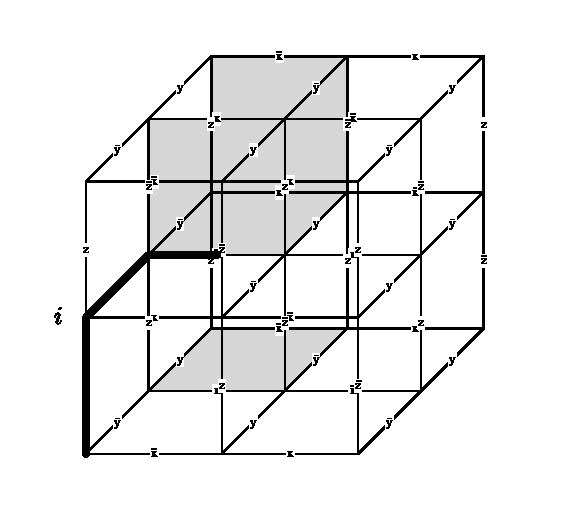
\includegraphics[width=0.72\textwidth]{fig_10.7.pdf}
\caption*{图 10.7\quad 立方格子中的一条开弦，以及与最近邻链相联系的指标对。开弦的一个端点翻转四个阴影方格上的 $F_{\pmb{p}}$ 的符号。}
\end{figure}
其中 $\sum_{\pmb{p}}$ 对立方格子的所有方格面求和。这里 $\pmb{i}_1$、$\pmb{i}_2$、$\pmb{i}_3$、$\pmb{i}_4$ 标记方格 $\pmb{p}$ 的四个角。引入复费米子算符
\begin{equation*}
2\psi_{1,\pmb{i}}=\lambda_{\pmb{i}}^{x}+\mathrm{i}\lambda_{\pmb{i}}^{\bar{x}}, \qquad 2\psi_{2,\pmb{i}}=\lambda_{\pmb{i}}^{y}+\mathrm{i}\lambda_{\pmb{i}}^{\bar{y}}, \qquad 2\psi_{3,\pmb{i}}=\lambda_{\pmb{i}}^{z}+\mathrm{i}\lambda_{\pmb{i}}^{\bar{z}},
\end{equation*}
并令 $N_{\pmb{i}}=\sum_{a=1,2,3}\psi_{a,\pmb{i}}^{\dagger}\psi_{a,\pmb{i}}$ 为格点 $\pmb{i}$ 上的费米子数算符。证明：在每个格点费米子数目为偶的子空间内，费米子哈密顿量 (10.5.6) 约化为自旋 $3/2$ 哈密顿量 (10.5.4)。
\item 用 10.2 节中的程序，求式 (10.5.4) 在具有周期性边界条件的偶数 $\times$ 偶数 $\times$ 偶数格子上的基态能量与基态简并度。
\end{enumerate}

\subsection{弦算符与闭合弦凝聚}

为了证明 $H_{3D}$ 的基态具有闭合弦凝聚，我们需要找到一个与 $H_{3D}$ 对易的闭合弦算符。首先，让我们构造更普遍的开弦算符。

为了用物理的 $\gamma^{ab}$ 算符构造弦算符，我们注意到，可以给每条最近邻链 $\pmb{i}\to\pmb{j}$ 联系一对指标 $ab$，如图 10.7 所示。例如，链 $\pmb{i}\to\pmb{i}+\pmb{x}$ 对应 $x\bar{x}$，链 $\pmb{i}\to\pmb{i}-\pmb{x}$ 对应 $\bar{x}x$，链 $\pmb{i}\to\pmb{i}+\pmb{y}$ 对应 $y\bar{y}$，等等。开弦
\begin{figure}[H]
\centering
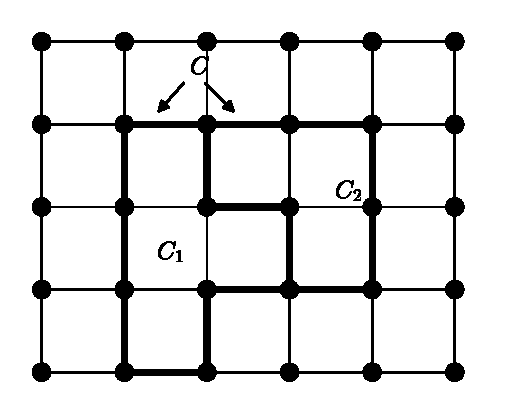
\includegraphics[width=0.72\textwidth]{fig_10.8.pdf}
\caption*{图 10.8\quad 回路 $C$ 可以分成两个回路 $C_1$ 与 $C_2$。}
\end{figure}
算符则定义为
\begin{equation*}
W(C)=-\left(-\mathrm{i}\gamma_{\pmb{i}_1}^{a_1b_1}\right)\left(-\mathrm{i}\gamma_{\pmb{i}_2}^{a_2b_2}\right)\dots\left(-\mathrm{i}\gamma_{\pmb{i}_n}^{a_nb_n}\right) \tag{10.5.7}
\end{equation*}
其中 $b_ma_{m+1}$ 是与链 $\pmb{i}_m\to\pmb{i}_{m+1}$ 相联系的指标对。例如，图 10.7 中那条开弦的开弦算符由下式给出：
\begin{equation*}
W(C)=-\left(-\mathrm{i}\gamma_{\pmb{i}}^{\bar{z}y}\right)\left(-\mathrm{i}\gamma_{\pmb{i}+\pmb{y}}^{\bar{y}x}\right)\left(-\mathrm{i}\gamma_{\pmb{i}+\pmb{x}+\pmb{y}}^{\bar{x}x}\right)
\end{equation*}
我们想强调，开弦 $C$ 是通过相邻格点把诸链的中点连接起来而构成的（见图 10.7）。因此，开弦的端点生活在链上。

闭合弦算符仍由式 (10.5.7) 给出，只是此时 $\pmb{i}_1$ 与 $\pmb{i}_n$ 为最近邻，并且 $b_na_1$ 是与链 $\pmb{i}_n\to\pmb{i}_1$ 相联系的指标对。

让我们先讨论导致闭合弦凝聚的闭合弦算符的一些特殊性质。利用 $\gamma^{ab}$ 的马约拉纳表示，可以证明任意两个闭合弦算符彼此对易。由于 $\hat F_{\pmb{p}}$ 本身就是一个闭合弦算符，闭合弦算符与自旋 $3/2$ 哈密顿量对易。因此，基态也是闭合弦算符的本征态，具有闭合弦凝聚（或更一般地，闭合弦网凝聚）。

如果我们把一个回路 $C$ 分成两个回路 $C_1$ 与 $C_2$（如图 10.8 那样），那么三个回路的闭合弦算符满足关系
\begin{equation*}
W(C)=W(C_1)W(C_2) \tag{10.5.8}
\end{equation*}
这一关系使我们能把 $W(C)$ 写成诸 $F_{\pmb{p}}$ 的乘积，从而计算凝聚闭合弦的振幅。对 $\hat F_{\pmb{p}}=1$ 的基态，我们发现
\begin{equation*}
\langle W(C_{\text{close}})\rangle=1
\end{equation*}
对 $\hat F_{\pmb{p}}=-1$ 的基态，我们发现
\begin{equation*}
\langle W(C_{\text{close}})\rangle=(-)^{N_{\pmb{p}}}
\end{equation*}
其中 $N_{\pmb{p}}$ 是曲面 $S_{C_{\text{close}}}$ 上方格的数目，而 $S_{C_{\text{close}}}$ 是由立方体的面组成、以闭合弦 $C_{\text{close}}$ 为边界的曲面。

\subsection*{问题 10.5.3}

\begin{enumerate}
\item 利用 $\gamma^{ab}=\mathrm{i}\lambda^{a}\lambda^{b}$ 的马约拉纳费米子表示，证明闭合弦算符 (10.5.7) 可以表示为
\begin{equation*}
W(C_{\text{close}})=\hat U_{\pmb{i}_1\pmb{i}_2}\hat U_{\pmb{i}_2\pmb{i}_3}\dots\hat U_{\pmb{i}_{n-1}\pmb{i}_n}\hat U_{\pmb{i}_n\pmb{i}_1}
\end{equation*}
其中 $\hat U_{\pmb{i}\pmb{j}}$ 的定义见式 (10.5.5)。
\item 证明对两个闭合回路定义的闭合弦算符 (10.5.7) 彼此对易。
\item 验证关系式 (10.5.8)。
\end{enumerate}

\subsection{作为开弦端点的演生费米子}

在闭合弦凝聚态中，开弦的端点成为一种新的准粒子。把开弦算符作用到一个基态上，通过计算 $F_{\pmb{p}}$ 与开弦算符之间的对易子可以发现，开弦算符只在其两个端点附近翻转 $F_{\pmb{p}}$ 的符号。因此，弦本身不耗费能量，只有弦端点耗费能量。

注意到弦端点生活在链上，而每条链连接着四个方格，我们发现开弦算符在这四个方格上翻转 $F_{\pmb{p}}$ 的符号（见图 10.7）。因此，开弦的每个端点对应一个小 $Z_2$ 通量圈，耗费能量 $4|2g|=8|g|$。这些小 $Z_2$ 通量圈对应于基态之上的准粒子激发。

为了求出 $Z_2$ 通量圈的统计性质，我们需要用到 Levin 与 Wen (2003) 引入的以下统计跳跃代数（见 4.1.4 节）：
\begin{align*}
&t_{jl}t_{kj}t_{ji}=\mathrm{e}^{\mathrm{i}\theta}t_{ji}t_{kj}t_{jl},\\
&[t_{ij},t_{kl}]=0, \qquad \text{若 } i,j,k,l \text{ 互不相同}, \tag{10.5.9}
\end{align*}
其中 $t_{ji}$ 描述粒子从链 $i$ 到链 $j$ 的跳跃（注意，这里弦的端点生活在链上）。已经证明，若粒子的跳跃算符满足 $\theta=\pi$ 的代数 (10.5.9)，则这些粒子是费米子。如果我们取 $(i,j,k,l)$
\begin{figure}[H]
\centering
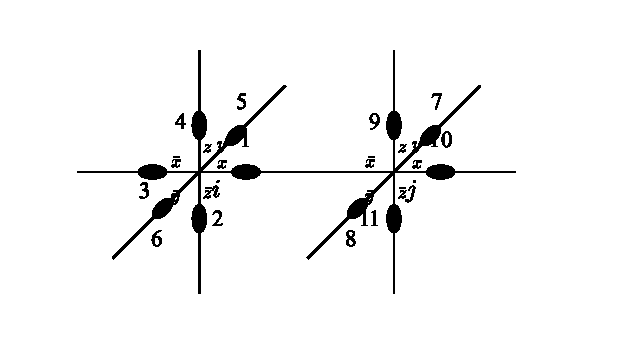
\includegraphics[width=0.72\textwidth]{fig_10.9.pdf}
\caption*{图 10.9\quad 链 1 上的一个费米子可以跳跃到十条不同的链 2--11 上。跳跃 $1\to4$ 由 $\gamma_{\pmb{i}}^{zx}$ 产生，跳跃 $1\to3$ 由 $\gamma_{\pmb{i}}^{\bar{x}x}$ 产生，跳跃 $1\to7$ 由 $\gamma_{\pmb{j}}^{y\bar{x}}$ 产生。}
\end{figure}
为图 10.9 中的链 $(2,1,3,4)$，那么跳跃算符 $(t_{jl},t_{kj},t_{ji})$ 由 $(\gamma_{\pmb{i}}^{xz},\gamma_{\pmb{i}}^{\bar{x}x},\gamma_{\pmb{i}}^{x\bar{z}})$ 给出。式 (10.5.9) 成为
\begin{equation*}
\gamma_{\pmb{i}}^{xz}\gamma_{\pmb{i}}^{\bar{x}x}\gamma_{\pmb{i}}^{x\bar{z}}=\mathrm{e}^{\mathrm{i}\theta}\gamma_{\pmb{i}}^{x\bar{z}}\gamma_{\pmb{i}}^{\bar{x}x}\gamma_{\pmb{i}}^{xz}
\end{equation*}
利用 $\gamma^{ab}$ 的马约拉纳费米子表示，我们发现上式在 $\theta=\pi$ 时成立。如果我们取 $(i,j,k,l)$ 为链 $(2,1,3,10)$，则式 (10.5.9) 成为
\begin{equation*}
\gamma_{\pmb{j}}^{\bar{x}x}\gamma_{\pmb{i}}^{\bar{x}x}\gamma_{\pmb{i}}^{x\bar{z}}=\mathrm{e}^{\mathrm{i}\theta}\gamma_{\pmb{i}}^{x\bar{z}}\gamma_{\pmb{i}}^{\bar{x}x}\gamma_{\pmb{j}}^{\bar{x}x}
\end{equation*}
上式同样在 $\theta=\pi$ 时成立。$(i,j,k,l)$ 的其他取法都属于上述两种类型。弦端点的跳跃满足费米子跳跃代数。因此，弦的端点（即小 $Z_2$ 通量圈）是费米子。我们看到，只要玻色模型具有某些类型闭合弦的凝聚，费米子就能从局域玻色模型中演生出来。

\section{量子转子模型与 $U(1)$ 格点规范理论}

\begin{keypoints}
\item 在更高维数，规范理论相当不平凡。它描述一个纠缠态的涨落，而这些涨落无法用局域自由度来表示。
\item $U(1)$ 规范涨落是空间中闭合弦网的涨落。
\item 如果基态包含任意尺寸闭合弦网的凝聚，就可以演生出无能隙的 $U(1)$ 规范玻色子。
\end{keypoints}

我们已经研究过具有演生 $Z_2$ 规范场的精确可解局域玻色模型。本节我们将从量子转子模型（quantum rotor model）出发，研究一个连续 $U(1)$ 规范理论的演生（Foerster et al., 1980; Senthil and Motrunich, 2002; Wen, 2003a）。
\begin{figure}[H]
\centering
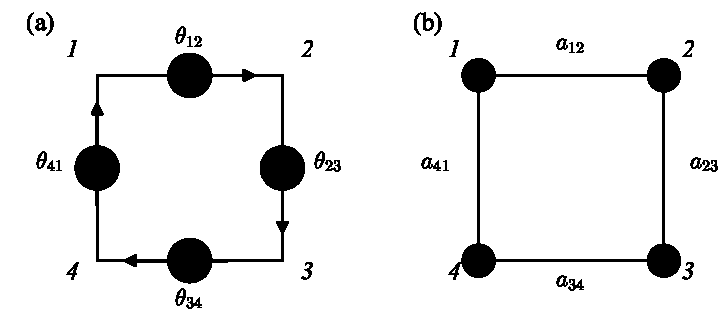
\includegraphics[width=0.72\textwidth]{fig_10.10.pdf}
\caption*{图 10.10\quad (a) 四转子系统。(b) 一个简单的格点规范理论，由格点规范场 $a_{i,i+1}$ 与 $a_0(i)$，$i=1,2,3,4$ 描述。}
\end{figure}
我们还将看到，弦网凝聚及相关的量子序如何与演生的 $U(1)$ 规范玻色子相联系。

本节也可以看作是对量子 $U(1)$ 规范理论的一种物理描述。在我看来，用规范势来描述规范理论的标准方式是不自然的，因为规范势本身是非物理的。这里我们将证明，可以用物理自由度——闭合弦网——来表述 $U(1)$ 规范理论（Banks et al., 1977; Savit, 1980）。

\subsection{四转子系统}

\begin{keypoints}
\item 转子角的某些组合的强量子涨落导致一个低能有效规范理论。
\end{keypoints}

让我们先考虑一个单转子：一个质量为 $m$ 的粒子在圆周 $0\leqslant\theta<2\pi$ 上运动。其拉格朗日量为
\begin{equation*}
L=\frac{1}{2}m\dot\theta^{2}+K\cos\theta
\end{equation*}
哈密顿量具有形式
\begin{equation*}
H=\frac{(S^{z})^{2}}{2m}-K\cos\theta=\frac{(S^{z})^{2}}{2m}-\frac{K}{2}(a+a^{\dagger})
\end{equation*}
其中 $S^{z}$ 是角动量，而 $a=\mathrm{e}^{-\mathrm{i}\theta}$。如果选取基底态 $|n\rangle=(2\pi)^{-1/2}\mathrm{e}^{\mathrm{i}n\theta}$（$n$ 取整数），则我们发现 $S^{z}|n\rangle=n|n\rangle$，$a|n\rangle=|n-1\rangle$。

为了得到具有演生低能规范理论的最简单模型，让我们考虑以下由 $\theta_{\langle12\rangle}$、$\theta_{\langle23\rangle}$、$\theta_{\langle34\rangle}$ 和 $\theta_{\langle41\rangle}$ 描述的四转子模型（见图 10.10(a)）：
\begin{equation*}
H=\sum_{i}\left(U\big(S_{\langle i-1,i\rangle}^{z}-S_{\langle i,i+1\rangle}^{z}\big)^{2}+J\big(S_{\langle i,i+1\rangle}^{z}\big)^{2}\right), \tag{10.6.1}
\end{equation*}
其中我们已约定 $4+1\sim1$，$1-1\sim4$。希尔伯特空间由 $|n_{\langle12\rangle}n_{\langle23\rangle}n_{\langle34\rangle}n_{\langle41\rangle}\rangle$ 张成，其中整数 $n_{i,i+1}$ 是 $S_{\langle i,i+1\rangle}^{z}$ 的本征值。若 $U\gg J$，则低能激发由能量 $E=4Jn^{2}$ 的 $|nnnn\rangle$ 态描述。所有其余激发的能量均为 $U$ 的量级。

为了看清它与格点规范理论的联系，我们想写出四转子模型的拉格朗日量。如果把哈密顿量写成 $H=\frac{1}{2}P^{\top}VP$ 的形式，其中 $P^{\top}=(S_{\langle12\rangle}^{z},S_{\langle23\rangle}^{z},S_{\langle34\rangle}^{z},S_{\langle41\rangle}^{z})$，而
\begin{equation*}
V=\begin{pmatrix}
4U+2J & -2U & 0 & -2U\\
-2U & 4U+2J & -2U & 0\\
0 & -2U & 4U+2J & -2U\\
-2U & 0 & -2U & 4U+2J
\end{pmatrix},
\end{equation*}
则拉格朗日量为
\begin{equation*}
L=\frac{1}{2}\dot\Theta^{\top}M\dot\Theta,
\end{equation*}
其中 $\Theta^{\top}=(\theta_{\langle12\rangle},\theta_{\langle23\rangle},\theta_{\langle34\rangle},\theta_{\langle41\rangle})$，$M=V^{-1}$。

显然，在上述拉格朗日量中我们看不到规范理论的任何迹象。为了得到规范理论，我们需要换一种方法导出拉格朗日量。利用 $H$ 的路径积分表示，并注意到 $(\theta,S^{z})$ 是一对正则坐标--动量，我们发现
\begin{equation*}
Z=\int\mathcal{D}S^{z}\,\mathcal{D}\theta\;\mathrm{e}^{\mathrm{i}\int\mathrm{d}t\,\big(\sum_{i}S_{\langle i,i+1\rangle}^{z}\dot\theta_{\langle i,i-1\rangle}-H\big)}
\end{equation*}
引入场 $a_0(i)$（$i=1,2,3,4$）来解耦 $U$ 项，可以把上述路径积分改写为
\begin{equation*}
Z=\int\mathcal{D}S^{z}\,\mathcal{D}\theta\,\mathcal{D}a_0\;\mathrm{e}^{\mathrm{i}\int\mathrm{d}t\,\big(\sum_{i}S_{\langle i,i+1\rangle}^{z}\dot\theta_{\langle i,i+1\rangle}-\tilde H(S^{z},a_0)\big)}
\end{equation*}
其中 $\tilde H=\sum_{i}\Big(J(S_{\langle i,i+1\rangle}^{z})^{2}+a_0(i)\big(S_{\langle i-1,i\rangle}^{z}-S_{\langle i,i+1\rangle}^{z}\big)-\frac{a_0^{2}(i)}{4U}\Big)$。积掉 $S_{\langle i,i+1\rangle}^{z}$ 后，我们得到
\begin{equation*}
Z=\int\mathcal{D}\theta\,\mathcal{D}a_0\;\mathrm{e}^{\mathrm{i}\int\mathrm{d}t\,L(\theta,\dot\theta,a_0)}
\end{equation*}
其中拉格朗日量为
\begin{equation*}
L=\frac{1}{4J}\sum_{i}\left(\big(\dot\theta_{\langle i,i+1\rangle}+a_0(i)-a_0(i+1)\big)^{2}+\frac{a_0^{2}(i)}{4U}\right)
\end{equation*}
在大 $U$ 极限下，可以丢掉 $a_0^{2}(i)/4U$ 项，得到
\begin{equation*}
L=\frac{1}{4J}\sum_{i}\big(\dot a_{i,i+1}+a_0(i)-a_0(i+1)\big)^{2}
\end{equation*}
这正是单个方格上 $U(1)$ 格点规范理论的拉格朗日量，其中
\begin{equation*}
a_{i,i+1}=\theta_{\langle i,i+1\rangle}, \qquad a_{i+1,i}=-\theta_{\langle i,i+1\rangle}
\end{equation*}
作为格点规范场（见图 10.10(b)）。可以检验，上述拉格朗日量在下列变换下不变：
\begin{equation*}
a_{ij}(t)\to a_{ij}(t)+\phi_{j}(t)-\phi_{i}(t), \qquad a_0(i,t)\to a_0(i,t)+\dot\phi_{i}(t) \tag{10.6.2}
\end{equation*}
这个变换称为规范变换。我们注意到，低能波函数 $\Psi(a_{12},a_{23},a_{34},a_{41})$ 是 $|nnnn\rangle$ 态的叠加。所有低能态都是规范不变的，即在规范变换 $a_{ij}\to a_{ij}+\phi_{j}-\phi_{i}$ 下不变。

连续 $U(1)$ 规范理论的电场由 $\pmb{E}=\pmb{\dot a}-\partial a_{0}$ 给出（取 $c=e=1$ 单位）。在格点规范理论中，电场变成定义在链上的如下量：
\begin{equation*}
E_{ij}=\dot a_{ij}-\big(a_0(j)-a_0(i)\big)
\end{equation*}
我们看到，我们的格点规范拉格朗日量可以写成 $L=\frac{1}{4J}\sum_{i}E_{i,i+1}^{2}$。把它与连续 $U(1)$ 规范理论 $\mathcal{L}\propto\pmb{E}^{2}-\pmb{B}^{2}$ 相比较，可见我们的拉格朗日量只包含对应于 $\pmb{E}^{2}$ 的动能。更普遍的格点规范理论还包含对应于 $\pmb{B}^{2}$ 的势能项。

为了得到势能项，我们把转子模型推广为
\begin{equation*}
\begin{split}
H=\sum_{i}\Big(&U\big(S_{\langle i-1,i\rangle}^{z}-S_{\langle i,i+1\rangle}^{z}\big)^{2}+J\big(S_{\langle i,i+1\rangle}^{z}\big)^{2}\\
&+t\big(\mathrm{e}^{\mathrm{i}\theta_{\langle i-1,i\rangle}}\mathrm{e}^{\mathrm{i}\theta_{\langle i,i+1\rangle}}+\text{h.c.}\big)\Big),
\end{split} \tag{10.6.3}
\end{equation*}
我们注意到 $\langle nnn|\mathrm{e}^{\mathrm{i}\theta_{\langle i-1,i\rangle}}\mathrm{e}^{-\mathrm{i}\theta_{\langle i,i+1\rangle}}|nnn\rangle=0$。因此，在 $t$ 的一阶，新项对低能没有影响。新项的低能效应只在 $t$ 的二阶才出现。

如果带着新项重复上述计算，就得到以下拉格朗日量：
\begin{equation*}
L=\frac{1}{4J}\sum_{i}\left(\big(\dot a_{i,i+1}+a_0(i)-a_0(i+1)\big)^{2}-t\big(\mathrm{e}^{\mathrm{i}(a_{i-1,i}+a_{i,i+1})}+\text{h.c.}\big)+\frac{a_0^{2}(i)}{4U}\right)
\end{equation*}
在上述拉格朗日量中，为什么新项在 $t$ 一阶下没有低能效应，稍微难看出来一些。让我们集中考虑如下形式的涨落：\footnote{在格点规范理论中，这种类型的涨落被称为纯规范涨落。}
\begin{equation*}
a_{i-1,i}=\phi_{i}-\phi_{i-1}
\end{equation*}
积掉 $a_0(i)$ 之后，这类涨落的拉格朗日量具有形式 $L=\frac{1}{2}\phi_{i}m_{ij}\phi_{j}-\sum_{i}t\big(\mathrm{e}^{\mathrm{i}(\phi_{i-1}+\phi_{i+1})}+\text{h.c.}\big)$，其中 $m_{ij}=O(U^{-1})$。我们看到，在大 $U$ 极限下，上述形式的涨落是快速而强烈的。由于 $\phi_{i}$ 生活在紧致空间上（即 $\phi_{i}$ 与 $\phi_{i}+2\pi$ 表示同一个点），这些快速涨落全都具有 $U$ 量级的大能隙。现在我们看到，$t$ 项 $t\,\mathrm{e}^{\mathrm{i}(\phi_{i-1}-\phi_{i+1})}$ 由于 $\phi_{i}$ 的强涨落而平均为零，在 $t$ 一阶下没有任何影响。然而，在 $t$ 的二阶，会出现一项 $t^{2}\prod_{i=1,3}\mathrm{e}^{\mathrm{i}(\theta_{\langle i-1,i\rangle}+\theta_{\langle i,i+1\rangle})}=t^{2}\mathrm{e}^{\mathrm{i}\sum_{i}a_{i-1,i}}$。这样的项不依赖于 $\phi_{i}$，因而不会平均为零。于是我们预期低能有效拉格朗日量具有如下形式：
\begin{equation*}
L=\frac{1}{4J}\sum_{i}\left(\big(\dot a_{i,i+1}+a_0(i)-a_0(i+1)\big)^{2}+\frac{a_0^{2}(i)}{4U}\right)+g\cos\Phi \tag{10.6.4}
\end{equation*}
其中 $g=O(t^{2}/U)$，而 $\Phi=\sum_{i}a_{i,i+1}$ 是 $U(1)$ 规范场穿过方格的通量。上述拉格朗日量不依赖快速量子涨落，并且在规范变换 (10.6.2) 下不变。我们看到，正是 $a_{ij}$ 的某些组合的强量子涨落，导致了一个规范不变的低能有效拉格朗日量。

为了定量地计算 $g$，我们先要导出低能有效哈密顿量。如果把 $t$ 项当作微扰来处理，并把低能态当作简并态，那么在 $t$ 的二阶，我们有
\begin{align*}
&\langle n_{1},n_{1},n_{1},n_{1}|H_{eff}|nnnn\rangle\\
&=-\frac{t^{2}}{2U}\langle n_{1},n_{1},n_{1},n_{1}|\mathrm{e}^{\mathrm{i}(\theta_{\langle34\rangle}+\theta_{\langle41\rangle})}|n_{1},n_{1},n,n\rangle\langle n_{1},n_{1},n,n|\mathrm{e}^{\mathrm{i}(\theta_{\langle12\rangle}+\theta_{\langle23\rangle})}|nnnn\rangle\\
&\quad+\text{另外三个类似的项}\\
&=-\frac{2t^{2}}{U}
\end{align*}
其中 $n_{1}=n+1$。于是，低能有效哈密顿量为
\begin{equation*}
H=\sum_{i}\left(U\big(S_{\langle i-1,i\rangle}^{z}-S_{\langle i,i+1\rangle}^{z}\big)^{2}+J\big(S_{\langle i,i+1\rangle}^{z}\big)^{2}\right)-\frac{4t^{2}}{U}\cos(\Phi).
\end{equation*}
相应的拉格朗日量由式 (10.6.4) 给出，其中
\begin{equation*}
g=\frac{4t^{2}}{U}.
\end{equation*}
如前所述，纯规范涨落具有 $U$ 量级的大能隙。$U$ 以下的低能有效理论可以令 $U\to\infty$ 得到，
\begin{figure}[H]
\centering
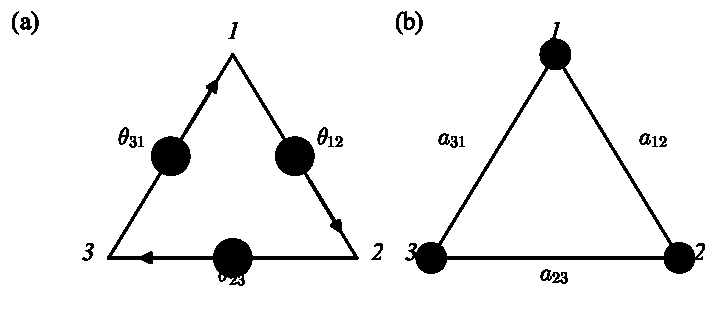
\includegraphics[width=0.72\textwidth]{fig_10.11.pdf}
\caption*{图 10.11\quad (a) 三转子系统；(b) 相关的格点规范理论。}
\end{figure}
并且我们得到
\begin{equation*}
L=\frac{1}{4J}\sum_{i}\big(\dot a_{i,i+1}+a_0(i)-a_0(i+1)\big)^{2}+g\cos\Phi \tag{10.6.5}
\end{equation*}

这个模型曾在 6.4 节中研究过。那里证明了，当 $g=0$ 时，能级为 $E_{n}=4Jn^{2}$，与式 (10.6.1) 的低能能级精确一致。因此，式 (10.6.1) 在低能下确实是一个规范理论。

这里我们想作一点评论。什么是规范理论？四转子模型在低能下真的是一个规范理论吗？规范理论的标准定义是含有规范势的理论。按照这个定义，如果我们坚持用规范势来写四转子模型的拉格朗日量，它就可以是一个规范理论。另一方面，四转子模型又不是规范理论，因为它的自然拉格朗日量不含有任何规范势。我们看到，规范理论并不是一个定义良好的物理概念。“一个模型是不是规范理论”并不是一个定义良好的问题。这几乎就像：如果我们把四个格点标记为 $(a,b,c,d)$，就管四转子模型叫规范理论；而如果我们把四个格点标记为 $(1,2,3,4)$，就管它叫非规范理论。从这个观点看，本节的讨论是相当形式化的，没有什么物理意义。

\subsection*{问题 10.6.1}

考虑式 (10.6.3) 所描述的 $i=1,2,3$ 三格点转子模型（见图 10.11）。

\begin{enumerate}
\item 导出低能格点规范理论的作用量。你只需把 $g$ 计算到 $O(1)$ 系数的精度。
\item 假定 $U\gg g\gg J$，计算低能下的能级。
\end{enumerate}

\subsection{量子转子格子与人工光}

\begin{keypoints}
\item 量子转子格子可以用一个格点 $U(1)$ 规范理论来描述。
\end{keypoints}

\begin{figure}[H]
\centering
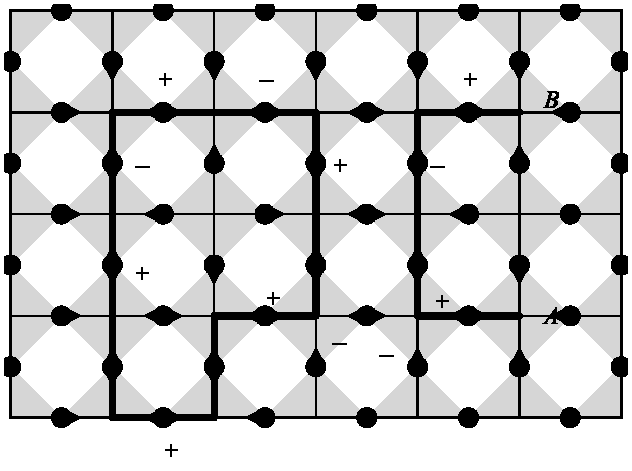
\includegraphics[width=0.72\textwidth]{fig_10.12.pdf}
\caption*{图 10.12\quad 转子格子、表示低能涨落的一个回路，以及一对电荷激发（A、B）。在大 $U$ 极限下，每个阴影方格四角处转子的角动量之和为零。}
\end{figure}

\begin{keypoints}
\item 格点规范理论的解禁闭相包含人工光（artificial light）。
\end{keypoints}

在理解了只含少数几个转子的系统之后，我们就可以着手研究格子转子系统了。作为一个例子，我们将考虑一个正方格子，每条链上有一个转子（见图 10.12）。我们有
\begin{align*}
H=U\sum_{\pmb{i}}\Bigg(\sum_{\pmb{\alpha}}S_{\pmb{i}+\pmb{\alpha}}^{z}\Bigg)^{2}&+J\sum_{\pmb{i},\pmb{\alpha}}\big(S_{\pmb{i}+\pmb{\alpha}}^{z}\big)^{2}+\sum_{\pmb{i}}\Big(t_{1}\,\mathrm{e}^{\mathrm{i}\big(\theta_{\pmb{i}+\frac{\pmb{x}}{2}}-\theta_{\pmb{i}+\frac{\pmb{y}}{2}}\big)}\\
&+t_{2}\,\mathrm{e}^{\mathrm{i}\big(\theta_{\pmb{i}+\frac{\pmb{y}}{2}}-\theta_{\pmb{i}-\frac{\pmb{x}}{2}}\big)}+t_{3}\,\mathrm{e}^{\mathrm{i}\big(\theta_{\pmb{i}-\frac{\pmb{x}}{2}}-\theta_{\pmb{i}-\frac{\pmb{y}}{2}}\big)}+t_{4}\,\mathrm{e}^{\mathrm{i}\big(\theta_{\pmb{i}-\frac{\pmb{y}}{2}}-\theta_{\pmb{i}+\frac{\pmb{x}}{2}}\big)}+\text{h.c.}\Bigg) \tag{10.6.6}
\end{align*}
这里 $\pmb{i}=(i_x,i_y)$ 标记正方格子的格点，而 $\pmb{\alpha}=\pm\frac{\pmb{x}}{2},\pm\frac{\pmb{y}}{2}$。$U$ 项强制施加了“格点 $\pmb{i}$ 附近四个转子的总角动量为零”这一约束。该模型还可以推广到三维立方格子：
\begin{align*}
H=U\sum_{\pmb{i}}\Bigg(&\sum_{\pmb{\alpha}}S_{\pmb{i}+\pmb{\alpha}}^{z}\Bigg)^{2}+J\sum_{\pmb{i},\pmb{\alpha}}\big(S_{\pmb{i}+\pmb{\alpha}}^{z}\big)^{2}\\
&+\sum_{\pmb{i},\langle\pmb{\alpha}_1\pmb{\alpha}_2\rangle}\left(t_{\langle\pmb{\alpha}_1\pmb{\alpha}_2\rangle}\,\mathrm{e}^{\mathrm{i}(\theta_{\pmb{i}+\pmb{\alpha}_1}-\theta_{\pmb{i}+\pmb{\alpha}_2})}+\text{h.c.}\right) \tag{10.6.7}
\end{align*}
这里 $\pmb{i}=(i_x,i_y,i_z)$ 标记立方格子的格点，$\pmb{\alpha}=\pm\frac{\pmb{x}}{2},\pm\frac{\pmb{y}}{2},\pm\frac{\pmb{z}}{2}$，而两个标记 $\pmb{i}+\pmb{\alpha}_1$ 与 $\pmb{i}+\pmb{\alpha}_2$ 表示绕 $\pmb{i}$ 格点的两个最近邻转子。

% 实际覆盖范围（以 PNG 为准）：本块不含 §10.5——§10.5、§10.6.1 及 §10.6.2 前半
% （书页 466–478）属 ch10_c 块；本块自 §10.6.2 中段（书页 479 顶）起，
% 至 §10.7.3 中段（书页 491 末）止。
% 块界说明：
%   起点——书页 479（p494）顶部 "In the following, we are going to show that..."
%   为新起段落，书页 478（p493）末句 "...the two nearest-neighbor rotors around
%   the i site." 已完整结束，故本块不设 %JOIN%，亦无 ch10_c 收尾内容可写入
%   %--C-TAIL-- 区。
%   终点——书页 491（p506）末句 "In the continuum limit, ... and B is the
%   magnetic field" 延续到书页 492（p507，ch10_e 块）顶部 "strength of the
%   U(1) gauge field. Comparing this with..."。按约定，半句译文（"……而 $\pmb B$ 是"）
%   留在本文件正文最末，未写入任何 TAIL 区；请 ch10_e 以 %JOIN% 起头续译
%   "该 $U(1)$ 规范场的磁场强度。把它与……"，勿重复勿遗漏。

下面我们将证明，在 $U\gg t$、$J$ 且 $t^{2}/U\gg J$ 的极限下，上述二维和三维模型都包含一个低能集体模式。由于其非局域的性质，这种集体模式与自旋波、声子这类通常的集体模式非常不同。实际上，它不对应于任何局域序参量的涨落，必须用 $U(1)$ 规范理论来描写。我们把这样的集体模式称为 $U(1)$ 规范涨落。该集体模式在二维模型中具有指数式小的能隙 $\Delta\sim\mathrm{e}^{-C\sqrt{t^{2}/JU}}$，在三维模型中则严格无能隙。三维模型中的集体模式在各个方面都表现得像我们宇宙中的光。因此，我们也可以称它为人工光。

上述模型引人注目之处在于，它们在格子尺度上没有任何规范结构的迹象。$U(1)$ 规范涨落及与之相联系的规范结构是在低能下演生的。这提示了一种可能：我们宇宙中的光或许也以类似的方式出现。规范结构可能会在强关联量子系统中自然地演生。本节要研究的转子模型是包含人工光的最简单模型。下面为简单起见，我们将集中于二维转子模型。计算与结果可以容易地推广到三维转子模型。

为了理解我们二维转子系统的动力学，让我们先设 $J=t=0$ 且 $U>0$。此时，哈密顿量由执行局域投影的对易项构成。基态高度简并，构成一个低能子空间。其中一个基态是每个转子的 $S^{z}_{\pmb i}=0$ 的态。其他基态可以从这个基态出发来构造：在正方格子上画一条有向回路，然后沿回路交替地把转子的角动量增加或减少 1（见图 10.12）。重复这一过程可以构造出所有简并基态。我们看到，投影空间中的涨落由回路表示。尽管低能子空间是通过局域投影得到的，它却带有一些非局域的特征。若 $t$ 与 $J$ 非零，则 $t$ 项会使这些回路涨落，而 $J$ 项会给这些回路正比于回路长度的能量。显然，当 $U\gg J,t$ 时，系统的低能性质由回路的涨落决定。系统可以有两个不同的相。当 $J\gg t$ 时，系统只有少许小回路涨落。当 $J\ll t$ 时，系统有许多大回路涨落，它们甚至可以充满整个空间。后面我们会看到，这些大回路涨落实际上正是 $U(1)$ 规范涨落。我们注意到，回路可以相交与交叠。实际上，一个典型的回路看起来更像一张闭合弦的网。下面，为强调这种涨落的分支结构，我们把回路涨落称为闭合弦网涨落。

简并基态在由
\begin{equation*}
U(\phi_{\pmb i})=\mathrm{e}^{\mathrm{i}\sum_{\pmb i}((-)^{\pmb i}\phi_{\pmb i}\sum_{\alpha}S^{z}_{\pmb i+\alpha})}\tag{10.6.8}
\end{equation*}
生成的局域对称变换下不变，其中 $(-)^{\pmb i}=(-)^{i_x+i_y}$。上述变换正是规范变换。因此，我们也可以说简并基态是规范不变的。

用与 10.6.1 小节相似的计算，我们发现我们的格子转子模型在大 $U$ 极限下可以用如下低能有效拉格朗日量描写：
\begin{equation*}
L=\frac{1}{4J}\sum_{\pmb i,\pmb\mu=\pmb x,\pmb y}[\dot{a}_{\pmb i,\pmb i+\pmb\mu}+a_0(\pmb i)-a_0(\pmb i+\pmb\mu)]^{2}+g\sum_{\pmb i}\cos(\Phi_{\pmb i})\tag{10.6.9}
\end{equation*}
这里 $a_{\pmb i,\pmb i+\pmb x}=(-)^{\pmb i}\theta_{\pmb i+\frac{\pmb x}{2}}$，$a_{\pmb i,\pmb i+\pmb y}=(-)^{\pmb i}\theta_{\pmb i+\frac{\pmb y}{2}}$，而 $a_{\pmb i\pmb j}=-a_{\pmb j\pmb i}$。另外，$\Phi_{\pmb i}$ 是通过 $\pmb i$ 处方格的 $U(1)$ 通量，即 $\Phi_{\pmb i}=a_{\pmb i,\pmb i+\pmb x}+a_{\pmb i+\pmb x,\pmb i+\pmb x+\pmb y}+a_{\pmb i+\pmb x+\pmb y,\pmb i+\pmb y}+a_{\pmb i+\pmb y,\pmb i}$。推广 10.6.1 小节的二阶微扰计算，我们得到
\begin{equation*}
g=2(t_1t_3+t_2t_4)/U.
\end{equation*}

式 (10.6.9) 描写一个 $U(1)$ 格点规范理论。

这里我们想强调，具有 $U(1)$ 规范理论形式的拉格朗日量 (10.6.9) 并不一定意味着低能激发的行为像规范玻色子。这是因为量子涨落可以非常强，来自拉格朗日量的直观图像可能完全造成误导。要有行为像规范玻色子的激发，我们需要选取 $J$ 与 $g$，使拉格朗日量 (10.6.9) 处于半经典极限。为了看清何时能够达到半经典极限，我们把格点规范理论的作用量写成如下无量纲形式：
\begin{equation*}
S=\sqrt{\frac{g}{J}}\int\mathrm{d}\tilde t\left(\frac{1}{4}\sum_{\pmb i,\pmb\mu=\pmb x,\pmb y}[\partial_{\tilde t}a_{\pmb i,\pmb i+\pmb\mu}+\tilde a_0(\pmb i)-\tilde a_0(\pmb i+\pmb\mu)]^{2}+\sum_{\pmb i}\cos(\Phi_{\pmb i})\right)
\end{equation*}
其中 $\tilde t=\sqrt{gJ}\,t$，$\tilde a_0=a_0/\sqrt{gJ}$。我们发现，当 $g/J=t^{2}/JU\gg1$ 时即达到半经典极限。在这一极限中，我们的模型包含 $U(1)$ 规范玻色子（即人工光）作为其唯一的低能集体激发。

由于瞬子效应，$U(1)$ 规范激发在 $1+2$ 维中会产生能隙（Polyakov, 1977）（见 6.3.2 小节）。瞬子效应与一个方格上 $U(1)$ 通量 $\Phi$ 从 0 到 $2\pi$ 的改变相联系。为了估计瞬子效应的重要性，让我们考虑只含单个方格的模型（即前面讨论过的四转子模型）。这样的模型由式 (6.4.11) 描写。瞬子效应对应于一条路径 $\Phi(t)$（依赖时间的通量），其中 $\Phi$ 从 $\Phi(-\infty)=0$ 变到 $\Phi(+\infty)=2\pi$。为了估计瞬子作用量，我们设
\begin{equation*}
\Phi(t)=\left\{\begin{array}{ll}0,&\text{当 } t<0\\ 2\pi t/T,&\text{当 } 0<t<T\\ 2\pi,&\text{当 } T<t\end{array}\right.
\end{equation*}
瞬子作用量的最小值为
\begin{equation*}
S_c=\pi\sqrt{g/J}
\end{equation*}
此时 $T=\pi/2\sqrt{gJ}$。由瞬子气体在时间轴上的密度 $\sqrt{Jg}\,\mathrm{e}^{-S_c}$，我们估计 $U(1)$ 规范玻色子的能隙为
\begin{equation*}
\Delta_{\mathrm{gauge}}\sim\sqrt{Jg}\,\mathrm{e}^{-\pi\sqrt{g/J}}\tag{10.6.10}
\end{equation*}

我们看到，当 $g/J\gg1$ 时，能隙可以非常小，低能涨落非常像无能隙的光子。当然，真正无能隙的人工光只存在于 $(3+1)$ 维模型中，例如三维转子模型 (10.6.7)。

三维转子模型在大 $U$ 极限下具有如下低能有效拉格朗日量：
\begin{equation*}
L=\frac{1}{4J}\sum_{\pmb i,\pmb\mu=\pmb x,\pmb y,z}[\dot{a}_{\pmb i,\pmb i+\pmb\mu}+a_0(\pmb i)-a_0(\pmb i+\pmb\mu)]^{2}+\sum_{\pmb p}g_{\pmb p}\cos(\Phi_{\pmb p})\tag{10.6.11}
\end{equation*}
这里 $\sum_{\pmb p}$ 对所有方格求和，$\Phi_{\pmb p}$ 是通过方格 $\pmb p$ 的 $U(1)$ 通量。另外，$g_{\pmb p}$ 可以依赖方格的取向，其数值可通过式 (10.6.7) 中的 $t_{\langle\pmb\alpha_1\pmb\alpha_2\rangle}$ 调节。

\subsection{人工光与人工电荷的弦网理论}

\begin{keypoints}
\item 规范理论是披着伪装的闭合弦网理论。
\item 禁闭相是具有稀疏小弦的相；库仑相是具有充满整个空间的大闭合弦网的相。
\item 规范玻色子（在库仑相中）对应于大闭合弦网的涨落，而规范电荷是开弦的端点。
\end{keypoints}

如前所述，我们的转子模型中 $U$ 以下的低能激发由 $S^{z}$ 增/减的闭合弦网描写。为了把这个图像弄得更精确，我们想在格子上定义一个弦网理论。

弦网理论的希尔伯特空间是我们转子模型 (10.6.6) 的希尔伯特空间的一个子空间。为了构造弦网希尔伯特空间，我们首先需要引入一个弦产生算符。弦产生算符由 $\mathrm{e}^{\pm\mathrm{i}\theta_{\langle\pmb i\pmb j\rangle}}$ 算符的乘积构成：
\begin{figure}[H]
\centering
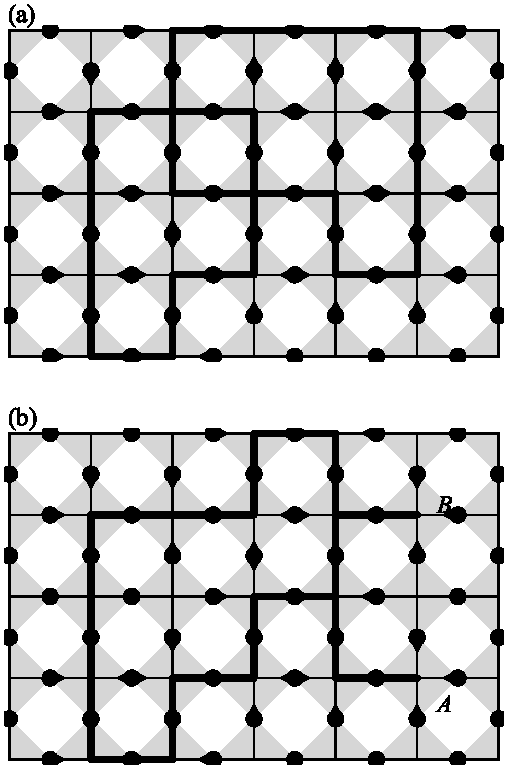
\includegraphics[width=0.72\textwidth]{fig_10.13.pdf}
\caption*{图 10.13\quad (a) 闭合弦网；(b) 开弦网。}
\end{figure}
\begin{equation*}
U(C)=\prod_{\langle\pmb i\pmb j\rangle}\mathrm{e}^{\mathrm{i}(-)^{\pmb i}\theta_{\langle\pmb i\pmb j\rangle}}\tag{10.6.12}
\end{equation*}
其中 $C$ 是连接正方格子上最近邻格点的一根弦，乘积 $\prod_{\langle\pmb i\pmb j\rangle}$ 遍历构成该弦的所有最近邻链 $\langle\pmb i\pmb j\rangle$，而 $\theta_{\langle\pmb i\pmb j\rangle}$ 是链 $\langle\pmb i\pmb j\rangle$ 上转子的 $\theta$ 场。

由于弦可以相交与交叠，弦看起来更像一张网。我们把 $C$ 称为弦网，把 $U(C)$ 称为弦网算符。若 $C$ 由一组闭合弦构成，我们就称它为闭合弦网；若 $C$ 至少含有一根开弦，就称它为开弦网（见图 10.13）。

弦网希尔伯特空间包含一个所有 $S^{z}_{\pmb I}=0$ 的态。按定义，这样的态对应于无弦态。如果我们把闭合弦算符 (10.6.12) 作用到 $S^{z}_{\pmb I}=0$ 态上，就得到弦网希尔伯特空间中的另一个态。这样的态由沿闭合弦 $C$ 的 $S^{z}_{\pmb I}=\pm1$ 构成，可以视为含一根闭合弦 $C$ 的态。弦网希尔伯特空间中的其他态对应于多弦态，可以通过反复把闭合弦算符 (10.6.12) 作用到 $S^{z}_{\pmb I}=0$ 态上产生。

我们弦网理论的哈密顿量由限制在弦网子空间中的转子哈密顿量 (10.6.6) 得到，其形式为
\begin{equation*}
H_{str}=\sum_{\langle\pmb i\pmb j\rangle}J(S^{z}_{\pmb i\pmb j})^{2}-\sum_{\pmb p}\frac{1}{2}(gW_{\pmb p}+h.c.)\tag{10.6.13}
\end{equation*}
其中求和 $\sum_{\langle\pmb i\pmb j\rangle}$ 遍历正方格子上所有最近邻链 $\langle\pmb i\pmb j\rangle$，$S^{z}_{\pmb i\pmb j}$ 是最近邻链 $\langle\pmb i\pmb j\rangle$ 上转子的角动量算符，$\sum_{\pmb p}$ 遍历正方格子的所有方格，而 $W_{\pmb p}$ 是绕方格 $\pmb p$ 的闭合弦的闭合弦算符。可以验证，上述哈密顿量确实作用在弦网希尔伯特空间之内。$J$ 项赋予弦网中的弦有限的弦张力，而 $g$ 项作为弦的“跳跃”项使弦网发生涨落。式 (10.6.13) 中的 $J$ 项直接来自式 (10.6.6) 中的 $J$ 项，而 $g$ 项来自式 (10.6.6) 中的 $t$ 项的二阶微扰展开。

由构造可以清楚地看到，弦网希尔伯特空间与我们的模型 (10.6.6) 的低能希尔伯特空间（由能量小于 $U$ 的态构成）恒同。由有效格点规范理论 (10.6.9) 的推导也同样清楚，弦网哈密顿量 (10.6.13) 与格点规范拉格朗日量 (10.6.9) 直接相关。实际上，格点规范理论的哈密顿量与弦网哈密顿量 (10.6.13) 恒同。弦网理论中的 $\sum_{\pmb i\pmb j}J(S^{z}_{\pmb i\pmb j})^{2}$ 项对应于规范理论中的 $\frac{1}{4J}\sum_{\langle\pmb i\pmb j\rangle}[\dot{a}_{\pmb i\pmb j}+a_0(\pmb i)-a_0(\pmb j)]^{2}$ 项，弦网理论中的 $\sum_{\pmb p}\frac{1}{2}g(W_{\pmb p}+h.c.)$ 项对应于规范理论中的 $g\sum_{\pmb p}\cos(\Phi_{\pmb p})$ 项。由于 $S^{z}\sim J^{-1}\dot{\theta}_{\langle\pmb i\pmb j\rangle}=J^{-1}\dot{a}_{\pmb i\pmb j}$ 对应于沿链的电通量，$S^{z}$ 增/减的闭合弦便对应于电通量管的一个回路。我们想强调，规范理论与弦网理论之间的上述联系不仅适用于二维模型 (10.6.6)，也适用于任何维数中的模型。

我们看到，$U(1)$ 规范理论 (10.6.9) 实际上是闭合弦网的一个动力学理论。通常人们期望闭合弦网的动力学理论像 (10.6.13) 那样用弦网写成。然而，由于我们更熟悉场论，前几节所做的事情可以视为用场论描写弦网理论的一种尝试。借助某些数学技巧，我们达到了目的：能够把弦网理论写成规范场论的形式。规范场论是一类特殊的场论，其中的场\emph{并不}对应于物理自由度，而且其物理希尔伯特空间是非局域的（即总物理希尔伯特空间不能写成局域希尔伯特空间的直积）。我们在这里想说明的要点是：规范理论（至少这里讨论的规范理论）是一种披着伪装的闭合弦网理论。换言之，规范理论与闭合弦网理论互为对偶。实际上，如果把时间离散化、考虑一个时空格子，我们就能找到 $U(1)$ 格点规范理论与时空中的膜的统计模型之间的精确映射（Banks et al., 1977; Savit, 1980）。

在大 $J/g$ 极限（因而是大 $\Delta_{\mathrm{gauge}}$ 极限）下，转子模型与弦网模型的基态都是每个转子 $S^{z}=0$ 的态。在这个相中，闭合弦网（或电通量管）涨落不大，能量正比于其长度。这意味着 $U(1)$ 规范理论处于禁闭相。在小 $J/g$ 极限下，闭合弦网强烈涨落，空间充满任意尺寸的闭合弦网。根据上一小节的计算，我们注意到小 $J/g$ 相也可以视为具有无能隙规范玻色子的库仑相。把这两幅图像结合起来，我们看到无能隙规范玻色子对应于大闭合弦网的涨落。

在把闭合弦网与人工光联系起来之后，我们现在转向人工电荷（artificial charge）。要为人造 $U(1)$ 规范场产生一对带相反人工电荷的粒子，我们需要画一根开弦，并沿弦交替地增减转子的 $S^{z}$（见图 10.12）。开弦的端点，作为电通量管的端点，对应于带相反人工电荷的粒子。我们注意到，与转子不同，带电粒子生活在正方格子的格点上。在禁闭相中，连接两个人工电荷的弦涨落不大，弦的能量正比于弦的长度。我们看到，人工电荷之间存在线性禁闭。

在小 $J/g$ 极限下，大的 $g$ 引起闭合弦网的强烈涨落，从而导致无能隙的 $U(1)$ 规范涨落。连接两个电荷的弦的强烈涨落还把线性禁闭势变为电荷之间的 $\log(r)$ 势。

为了理解带人工电荷的粒子的动力学并导出 $\log(r)$ 势，让我们导出这些带电粒子的低能有效理论。让我们先设 $J=t=0$。把开弦算符 (10.6.12) 作用到基态上，可以产生一对带相反单位人工电荷的带电粒子。在开弦的端点处，$(\sum_{\alpha}S^{z}_{\pmb i+\alpha})^{2}=1$。我们发现每个带电粒子具有能量 $U$，它来自 $U\sum_{\pmb i}(\sum_{\alpha}S^{z}_{\pmb i+\alpha})^{2}$ 这一项。弦本身不耗费能量。如果把同一开弦算符作用 $n$ 次，就在开弦的端点产生 $n$ 个单位的相反人工电荷。$n$ 个单位电荷的能量是 $n^{2}U$。

含电荷的规范理论包含两部分，即电荷与弦。让我们先只考虑电荷，把带电粒子当作独立粒子处理。此时，带电粒子的总希尔伯特空间由态 $|\{n_{\pmb i}\}\rangle$ 构成，其中 $n_{\pmb i}$ 是正方格子格点 $\pmb i$ 上人工电荷的数目。这里 $|\{n_{\pmb i}\}\rangle$ 是一个能量本征态，能量为 $E=U\sum_{\pmb i}n^{2}_{\pmb i}$。这样的系统可以用拉格朗日量
\begin{equation*}
L=\sum_{\pmb i}\frac{1}{4U}\dot{\varphi}^{2}_{\pmb i}\tag{10.6.14}
\end{equation*}
描写，其中 $\varphi_{\pmb i}$ 是一个角变量。产生单位电荷带电粒子的算符是 $\mathrm{e}^{\mathrm{i}\varphi_{\pmb i}}$。

规范涨落由弦和式 (10.6.9) 描写。在 $U(1)$ 规范理论中，基态是规范不变的（在远离电荷处）。由式 (10.6.8) 可见，规范不变性意味着 $\sum_{\alpha}S^{z}_{\pmb i+\alpha}=0$。因此在远离电荷处没有弦的开端。

为了找到电荷与规范场的耦合理论，我们把带电粒子总是处在开弦端点这一事实包括进来。换言之，规范理论的物理态包含开弦，但开弦只能终止在电荷上。这一约束可以由规范不变性施加。于是我们可以利用规范不变性，把电荷拉格朗日量 (10.6.14) 与规范拉格朗日量 (10.6.9) 合在一起，写出耦合理论。利用规范不变性，我们发现组合拉格朗日量具有如下形式（见问题 6.4.5）：
\begin{equation*}
L=\sum_{\pmb i}\frac{(\dot{\varphi}_{\pmb i}+a_0(\pmb i))^{2}}{4U}+\sum_{\pmb i,\pmb\mu=\pmb x,\pmb y}\frac{[\dot{a}_{\pmb i,\pmb i+\pmb\mu}+a_0(\pmb i)-a_0(\pmb i+\pmb\mu)]^{2}}{4J}+g\sum_{\pmb i}\cos(\Phi_{\pmb i})
\end{equation*}
把规范场包括进来之后，单电荷产生算符 $\mathrm{e}^{\mathrm{i}\varphi_{\pmb i}}$ 不再是物理的，因为它不是规范不变的。规范不变的算符
\begin{equation*}
\mathrm{e}^{-\mathrm{i}\varphi_{\pmb i_1}}\mathrm{e}^{\mathrm{i}a_{\pmb i_1\pmb i_2}}\mathrm{e}^{\mathrm{i}a_{\pmb i_2\pmb i_3}}\dots\mathrm{e}^{\mathrm{i}a_{\pmb i_{N-1}\pmb i_N}}\mathrm{e}^{\mathrm{i}\varphi_{\pmb i_N}}
\end{equation*}
总是产生一对相反电荷，连同连接两电荷的开弦。因此，开弦总是终止在电荷上。实际上，上述规范不变算符正是开弦算符 (10.6.12)。我们还看到，弦算符 (10.6.12) 与 Wegner--Wilson 圈算符密切相关（Wegner, 1971; Wilson, 1974; Kogut, 1979）。

$t$ 项产生带电粒子在正方格子上次近邻之间的跳跃。因此，若 $t\neq0$，带电粒子将具有非平庸的色散。相应的拉格朗日量为
\begin{equation*}
L=\sum_{\pmb i}\frac{(\dot{\varphi}_{\pmb i}+a_0(\pmb i))^{2}}{4U}-\sum_{\langle\pmb i\pmb j\rangle,a=1,2}t(\mathrm{e}^{\mathrm{i}(\varphi_{\pmb i}-\varphi_{\pmb j}-a_{\pmb i\pmb k_a}-a_{\pmb k_a\pmb j})}+h.c.)\tag{10.6.15}
\end{equation*}
其中 $\langle\pmb i\pmb j\rangle$ 是正方格子上的次近邻，$\pmb k_{1,2}$ 是格点 $\pmb i$ 与 $\pmb j$ 之间的两个格点。上述拉格朗日量还告诉我们，带电粒子是玻色子。

我们还注意到，$S^{z}_{\pmb i\pmb j}$ 的增加对应于 $\pmb i$ 与 $\pmb j$ 处的两个人工电荷。因此，每一单位人工电荷携带 1/2 角动量！（注意，总角动量 $\sum_{\langle\pmb i\pmb j\rangle}S^{z}_{\langle\pmb i\pmb j\rangle}$ 是守恒量。）

\subsection{二维与三维转子系统的物理性质}

\begin{keypoints}
\item 格点规范理论的连续极限。
\item 人工光的速度与精细结构常数。
\end{keypoints}

为了理解二维模型中人工光的物理性质，让我们按如下方式取式 (10.6.9) 的连续极限：
\begin{equation*}
a_{\pmb i\pmb j}=\delta\pmb x_{\langle\pmb i\pmb j\rangle}\cdot\pmb a(\pmb x),\qquad a_0(\pmb i)=a_0(\pmb x),
\end{equation*}
其中 $\pmb a=(a_x,a_y)$ 是一个二维矢量场（二维中的矢量规范势），$a_0$ 对应于势场，$\pmb x$ 取在格点 $\pmb i$ 附近，$\delta\pmb x_{\langle\pmb i\pmb j\rangle}$ 是连接正方格子上 $\pmb i$ 与 $\pmb j$ 两格点的矢量，而 $l$ 是正方格子的晶格常数。在连续极限下，拉格朗日量 (10.6.9) 变为
\begin{equation*}
L=\int\mathrm{d}^{2}\pmb x\ \left(\frac{1}{4J}\pmb e^{2}-\frac{gl^{2}}{2}\pmb b^{2}\right)\tag{10.6.16}
\end{equation*}
其中 $\pmb e=\partial_t\pmb a-\partial_{\pmb x}a_0$ 与 $\pmb b=\partial_x a_y-\partial_y a_x$ 分别是相应的仿造电场与仿造磁场。我们看到，人工光的速度为 $c_a=\sqrt{2gJl^{2}/h^{2}}$，人工光的带宽约为 $E_a=2c_a\hbar/l=\sqrt{8gJ}$。

由式 (10.6.15)，我们得到描写二维模型中带电粒子（在 $U\gg t$ 极限下）的连续拉格朗日量：
\begin{align*}
L=\int\mathrm{d}^{2}\pmb x\ \sum_{I=1,2}\Big(\phi^{\dagger}_{I}&(\mathrm{i}\partial_t-a_0-U)\phi_I-\frac{8tl^{2}}{2}\big|(\partial_{i}+\mathrm{i}a_{i})\phi_I\big|^{2}\\
+\bar{\phi}^{\dagger}_{I}&(\mathrm{i}\partial_t+a_0-U)\bar{\phi}_I-\frac{8tl^{2}}{2}\big|(\partial_{i}-\mathrm{i}a_{i})\bar{\phi}_I\big|^{2}\Big)
\end{align*}
（译注：原文两处时间导数下标印作 $\partial_l$，应为 $\partial_t$，此处已按本意译出。）

其中 $\phi_I$ 描写带正电的玻色子，$\bar{\phi}_I$ 描写带负电的玻色子，$\psi_1$ 与 $\bar{\psi}_1$ 描写正方格子偶格点上带电的玻色子，$\psi_2$ 与 $\bar{\psi}_2$ 描写奇格点上带电的玻色子。产生一对带电玻色子耗费能量 $2U$。玻色子的质量为 $m=(8tl^{2})^{-1}$，且 $mc_a^{2}=gJ/4t$。我们想指出，玻色子速度 $\sim 8tl$ 可以大于人工光的速度。正电荷与负电荷之间的势能为 $V(r)=\frac{2J}{\pi}\ln r$。

对于三维模型，连续极限下的拉格朗日量为
\begin{equation*}
L=\int\mathrm{d}^{3}\pmb x\ \left(\frac{1}{4Jl}\pmb e^{2}-\frac{gl}{2}\pmb b^{2}\right)\tag{10.6.17}
\end{equation*}
其中 $\pmb e$ 与 $\pmb b$ 分别是三维中的仿造电场与仿造磁场。人工光的速度为 $c_a=\sqrt{2gJl^{2}/h^{2}}$。上述三维拉格朗日量可以改写成更标准的形式
\begin{equation*}
L=\int\mathrm{d}^{3}\pmb x\ \frac{1}{8\pi\alpha}\left(\frac{1}{c_a}\pmb e^{2}-c_a\pmb b^{2}\right)\tag{10.6.18}
\end{equation*}
其中 $\alpha=\frac{1}{2\pi}\sqrt{J/2g}$ 是人工精细结构常数。带电玻色子的质量为 $m=(8tl^{2})^{-1}$。人工原子（artificial atom，即一个带正电玻色子与一个带负电玻色子的束缚态）具有 $\frac{1}{4}mc_a^{2}\alpha^{2}$ 量级的能级间距和 $2/\alpha mc_a$ 量级的尺寸。

\subsection*{问题 10.6.2}

验证式 (10.6.16) 与 (10.6.17)。

\section{从 $SU(N_f)$ 自旋模型演生的光与电子}

\begin{keypoints}
\item 局域玻色模型中非平庸的量子序（即弦网凝聚）可以同时导致无质量的光子与无质量的费米子。弦网凝聚提供了统一光与费米子的一条途径。
\item 光子与费米子的无质量性由刻画弦网凝聚的 PSG 保护。
\end{keypoints}

正如本章开头所强调的，理解光与电子的存在，就是理解这些粒子为什么是无质量的（与 Planck 质量相比近乎无质量）。对于一个一般的相互作用系统，无质量（即无能隙）激发是罕见的。如果它们存在，那么它们的存在必有原因。

我们知道，对称性破缺能够产生并保护无能隙的 Nambu--Goldstone 模。9.10 节中提出，除对称性破缺之外，量子序及与之相联系的 PSG 也能产生并保护无能隙激发。由量子序产生并保护的无能隙激发可以是无能隙规范玻色子和/或无能隙费米子。

在本节中，我们将研究立方格子上一个具体的 $SU(N_f)$ 自旋模型（Wen, 2002a）。该模型的基态具有非平庸的量子序（即弦网凝聚）。结果，模型具有演生的无质量 $U(1)$ 规范玻色子（人工光）以及无质量的带电费米子（人工电子与质子）。换言之，$SU(N_f)$ 自旋模型具有一个演生的 QED！基于这种 $SU(N_f)$ 自旋模型的世界将与我们自己的世界十分相似；两个世界都由通过库仑相互作用耦合的带电费米子（即电子与质子）构成。更复杂的立方格子自旋模型甚至可以导致含有光子、胶子、轻子和夸克的演生 QED 与 QCD（Wen, 2003b）。因此，如果有一天我们发现自然界中所有基本粒子都从一个推广的自旋模型（即局域玻色模型）中演生出来，那也不足为奇。

\subsection{立方格子上的 $SU(N_f)$ 自旋模型}

该模型由 $SU(N_f)$ 自旋构成，立方格子的每个格点上放有一个自旋。这里 $N_f$ 为偶数，格点用三个整数标记，即 $\pmb i=(i_x,i_y,i_z)$。每个格点上的态
\begin{equation*}
|a_1,a_2,\dots,a_{N_f/2}\rangle,\qquad a_1,\dots,a_{N_f/2}=1,2,\dots,N_f
\end{equation*}
构成 $SU(N_f)$ 的秩为 $N_f/2$ 的反对称张量表示。每个格点上的自旋算符 $S^{a\bar b}_{\pmb i}$（$a,\bar b=1,2,\dots,N_f$）构成 $SU(N_f)$ 的伴随表示：
\begin{gather*}
[S^{a\bar b}_{\pmb i},S^{c\bar d}_{\pmb i}]=\delta^{\bar b c}S^{a\bar d}_{\pmb i}-\delta^{a\bar d}S^{c\bar b}_{\pmb i}\\
S^{a\bar b}_{\pmb i}\delta_{a\bar b}=0\\
(S^{a\bar b}_{\pmb i})^{\dagger}=S^{\bar b a}_{\pmb i}\tag{10.7.1}
\end{gather*}
其中重复指标意味着求和。

令
\begin{equation*}
W_{\pmb i}=-N_f^{-4}S^{ab}_{\pmb i+\pmb x}S^{bc}_{\pmb i+\pmb x+\pmb y}S^{cd}_{\pmb i+\pmb y}S^{da}_{\pmb i}
\end{equation*}
我们把 $SU(N_f)$ 模型的哈密顿量取为（Wen, 2002a）
\begin{equation*}
H=g\sum_{\pmb i}[W_{\pmb i}+h.c]\tag{10.7.2}
\end{equation*}

\subsection{$SU(N_f)$ 模型的基态}

为理解基态，让我们引入 $SU(N_f)$ 自旋模型的费米子表示（Affleck and Marston, 1988）。我们先引入构成 $SU(N_f)$ 基础表示的 $N_f$ 个费米子算符 $\psi_a$。每个格点上的希尔伯特空间于是由具有 $N_f/2$ 个费米子的态构成。自旋算符由下式给出：
\begin{equation*}
S^{a\bar b}=\psi_a\psi^{\dagger}_{\bar b}-\frac{1}{2}\delta_{a\bar b}
\end{equation*}
如果我们引入
\begin{equation*}
\hat\chi_{\pmb i\pmb j}=N_f^{-1}\psi^{\dagger}_{a\pmb i}\psi_{a\pmb j}
\end{equation*}
则 $W_{\pmb i}$ 由下式给出：
\begin{equation*}
W_{\pmb i}=\hat\chi_{\pmb i,\pmb i+\pmb x}\hat\chi_{\pmb i+\pmb x,\pmb i+\pmb x+\pmb y}\hat\chi_{\pmb i+\pmb x+\pmb y,\pmb i+\pmb y}\hat\chi_{\pmb i+\pmb y,\pmb i}+O(1/N_f)
\end{equation*}
利用费米子表示，我们可以把哈密顿量 (10.7.2) 写成
\begin{equation*}
H=g\sum_{\pmb p}\Big[\prod_{\square}\hat\chi_{\pmb i\pmb j}+h.c.\Big]+O(N_f^{-1})\tag{10.7.3}
\end{equation*}
其中 $\sum_{\pmb p}$ 对所有方格 $\pmb p$ 求和，$\prod_{\square}$ 对方格 $\pmb p$ 周围的四条链求积；也就是说，$\prod_{\square}\hat\chi_{\pmb i\pmb j}\allowbreak=\hat\chi_{\pmb i_1\pmb i_2}\allowbreak\hat\chi_{\pmb i_2\pmb i_3}\allowbreak\hat\chi_{\pmb i_3\pmb i_4}\allowbreak\hat\chi_{\pmb i_4\pmb i_1}$，其中 $\pmb i_1,\pmb i_2,\pmb i_3,\pmb i_4$ 是方格 $\pmb p$ 周围的四个格点。

我们注意到，在大 $N_f$ 极限下，$\hat\chi_{\pmb i\pmb j}$ 彼此对易，即 $[\hat\chi_{\pmb i\pmb j},\hat\chi_{\pmb i'\pmb j'}]=O(1/N_f)$。另外，$\hat\chi_{\pmb i\pmb j}$ 是 $N_f$ 项之和。尽管每一项都有很强的量子涨落，其和却几乎没有涨落。因此，在大 $N_f$ 极限下 $\hat\chi_{\pmb i\pmb j}$ 的行为像一个 c 数。也就是说，对一个给定的态，我们可以把 $\hat\chi_{\pmb i\pmb j}$ 换成一个复数 $\chi_{\pmb i\pmb j}$。这样的态的能量为 $E=g\sum_{\pmb p}[\prod_{\square}\chi_{\pmb i\pmb j}+h.c.]+O(N_f^{-1})$。不同的态有不同的 $\chi_{\pmb i\pmb j}$，因而有不同的能量。

$SU(N_f)$ 模型的基态可以这样得到：选取一组使 $E=g\sum_{\pmb p}[\prod_{\square}\chi_{\pmb i\pmb j}+h.c.]$ 极小的 $\chi_{\pmb i\pmb j}$。这里我们遇到一个困难：$\chi_{\pmb i\pmb j}$ 并不独立，我们不能任意选取它们的值。例如，我们不能让所有 $\chi_{\pmb i\pmb j}$ 同时为零。我们将用 9.1.1 小节中的投影构造\footnote{9.1.1 小节中的讨论针对的是 $N_f=2$ 的 $SU(N_f)$ 模型。}来克服这一困难。我们从平均场哈密顿量
\begin{equation*}
H_{\mathrm{mean}}=-\sum_{\langle\pmb i\pmb j\rangle}\tilde\chi^{\dagger}_{\pmb i\pmb j}\psi^{\dagger}_{\pmb i}\psi_{\pmb j}+\sum_{\pmb i}a_0(\pmb i)\psi^{\dagger}_{\pmb i}\psi_{\pmb i}
\end{equation*}
出发。我们这样选取 $a_0(\pmb i)$，使得 $H_{\mathrm{mean}}$ 的平均场基态，即 $|\Psi^{\{\tilde\chi_{\pmb i\pmb j}\}}_{\mathrm{mean}}\rangle$，平均每格点拥有 $N_f/2$ 个费米子。$SU(N_f)$ 模型的态可以由平均场态 $|\Psi^{\{\tilde\chi_{\pmb i\pmb j}\}}_{\mathrm{mean}}\rangle$ 投影到每格点恰有 $N_f/2$ 个费米子的子空间中来构造：
\begin{equation*}
|\Psi^{\{\tilde\chi_{\pmb i\pmb j}\}}\rangle=\mathcal P|\Psi^{\{\tilde\chi_{\pmb i\pmb j}\}}_{\mathrm{mean}}\rangle
\end{equation*}
现在我们可以选取 $\tilde\chi_{\pmb i\pmb j}$，使平均能量 $\langle\Psi^{\{\tilde\chi_{\pmb i\pmb j}\}}|H|\Psi^{\{\tilde\chi_{\pmb i\pmb j}\}}\rangle$ 极小，从而得到基态的尝试能量与尝试波函数。

在大 $N_f$ 极限下，投影 $\mathcal P$ 只使波函数 $|\Psi^{\{\tilde\chi_{\pmb i\pmb j}\}}_{\mathrm{mean}}\rangle$ 发生很小的改变。因此，为得到基态能量，我们可以转而做一件更容易的计算：求 $\langle\Psi^{\{\tilde\chi_{\pmb i\pmb j}\}}_{\mathrm{mean}}|H|\Psi^{\{\tilde\chi_{\pmb i\pmb j}\}}_{\mathrm{mean}}\rangle$ 的极小。

极小化按如下步骤进行。我们先挑出一组 $\tilde\chi_{\pmb i\pmb j}$，然后选取 $a_0(\pmb i)$ 使得 $\langle\Psi^{\{\tilde\chi_{\pmb i\pmb j}\}}_{\mathrm{mean}}|\psi^{\dagger}_{\pmb i}\psi_{\pmb i}|\Psi^{\{\tilde\chi_{\pmb i\pmb j}\}}_{\mathrm{mean}}\rangle=N_f/2$，接着计算 $\chi_{\pmb i\pmb j}=N_f^{-1}\langle\Psi^{\{\tilde\chi_{\pmb i\pmb j}\}}_{\mathrm{mean}}|\psi^{\dagger}_{\pmb i}\psi_{\pmb j}|\Psi^{\{\tilde\chi_{\pmb i\pmb j}\}}_{\mathrm{mean}}\rangle$。这些 $\chi_{\pmb i\pmb j}$ 就是上面讨论过的算符 $\hat\chi_{\pmb i\pmb j}$ 所对应的 c 数。我们看到，$\tilde\chi_{\pmb i\pmb j}$ 是独立的，其值可以任意选取。非独立的 $\chi_{\pmb i\pmb j}$ 是 $\tilde\chi_{\pmb i\pmb j}$ 的函数，即 $\chi_{\pmb i\pmb j}(\{\tilde\chi_{\pmb i\pmb j}\})$。基态通过在改变 $\tilde\chi_{\pmb i\pmb j}$ 的同时使 $E=g\sum_{\pmb p}[\prod_{\square}\chi_{\pmb i\pmb j}(\{\tilde\chi_{\pmb i\pmb j}\})+h.c.]$ 极小而得到。

我们发现，基态可以通过如下选取 $\tilde\chi_{\pmb i\pmb j}$ 得到：
\begin{align*}
\tilde\chi_{\pmb i,\pmb i+\hat{\pmb x}}&\equiv-\mathrm{i}, & \tilde\chi_{\pmb i,\pmb i+\hat{\pmb y}}&\equiv-\mathrm{i}(-)^{i_x},\\
\tilde\chi_{\pmb i,\pmb i+\hat{\pmb z}}&\equiv-\mathrm{i}(-)^{i_x+i_y}, & a_0(\pmb i)&=0
\end{align*}
它引导出如下一组 $\chi_{\pmb i\pmb j}$：
\begin{align*}
\bar\chi_{\pmb i,\pmb i+\hat{\pmb x}}&\equiv-\mathrm{i}|\chi|, & \bar\chi_{\pmb i,\pmb i+\hat{\pmb y}}&\equiv-\mathrm{i}(-)^{i_x}|\chi|,\\
\bar\chi_{\pmb i,\pmb i+\hat{\pmb z}}&\equiv-\mathrm{i}(-)^{i_x+i_y}|\chi| & a_0(\pmb i)&=0.\tag{10.7.4}
\end{align*}
拟设 $\bar\chi_{\pmb i\pmb j}$ 在每个方格中都有 $\pi$ 通量。结果是 $\prod_{\square}\chi_{\pmb i\pmb j}=-|\chi|^{4}$。正是这个负号使上述 $\chi_{\pmb i\pmb j}$ 极小化 $g\sum_{\pmb p}[\prod_{\square}\chi_{\pmb i\pmb j}+h.c.]$（假定 $g>0$）。

由拟设 $\bar\chi_{\pmb i\pmb j}$ 描写的基态不破坏任何对称性。然而，该基态具有非平庸的量子序。下面我们将证明，基态支持无质量的 $U(1)$ 规范玻色子与无质量的带电费米子。

\subsection{$SU(N_f)$ 模型的低能动力学}

$\chi_{\pmb i\pmb j}$ 的涨落描写我们 $SU(N_f)$ 自旋模型中的一个集体模式。这一集体模式的动力学由立方格子上的一个经典场论描写。$|\chi|$ 的涨落对应于一种有质量的激发，可以忽略。集体模式的低能涨落由围绕 $\bar\chi_{\pmb i\pmb j}$ 的相位涨落描写，即 $\chi_{\pmb i\pmb j}=\bar\chi_{\pmb i\pmb j}\mathrm{e}^{\mathrm{i}a_{\pmb i\pmb j}}$。如 9.1.1 小节所讨论的，由 $a_{\pmb i\pmb j}$ 描写的涨落是 $U(1)$ 规范涨落。$U(1)$ 规范涨落的物理波函数由变形拟设的投影平均场态给出：
\begin{equation*}
\mathcal P|\Psi^{\{\bar\chi_{\pmb i\pmb j}\mathrm{e}^{\mathrm{i}a_{\pmb i\pmb j}}\}}_{\mathrm{mean}}\rangle.\tag{10.7.5}
\end{equation*}

把上式代入式 (10.7.3)，就得到 $a_{\pmb i\pmb j}$ 的如下有效哈密顿量：
\begin{equation*}
H=-2g\sum_{\pmb p}|\chi|^{4}\cos(\Phi_{\pmb p})\tag{10.7.6}
\end{equation*}
其中
\begin{equation*}
\Phi_{\pmb p}=a_{\pmb i_1\pmb i_2}+a_{\pmb i_2\pmb i_3}+a_{\pmb i_3\pmb i_4}+a_{\pmb i_4\pmb i_1}
\end{equation*}
而 $(\pmb i_1,\pmb i_2,\pmb i_3,\pmb i_4)$ 是方格 $\pmb p$ 周围的四个格点。哈密顿量 (10.7.6) 描写一个 $U(1)$ 格点规范理论：$a_{\pmb i\pmb j}$ 是格点 $U(1)$ 规范场，$\Phi_{\pmb p}$ 是通过方格 $\pmb p$ 的 $U(1)$ 通量。

$U(1)$ 规范涨落 (10.7.5) 不是唯一类型的低能激发。第二类低能激发由带有若干粒子--空穴激发的投影平均场态给出，例如
\begin{equation*}
\mathcal P\psi^{a}_{\pmb i_1}\psi^{b\dagger}_{\pmb i_2}|\Psi^{\{\bar\chi_{\pmb i\pmb j}\}}_{\mathrm{mean}}\rangle.\tag{10.7.7}
\end{equation*}
这些激发对应于带电费米子。

为确定费米子激发的动力学，我们写出
\begin{equation*}
\hat\chi_{\pmb i\pmb j}=\bar\chi_{\pmb i\pmb j}+N_f^{-1}:\psi^{\dagger}_{a,\pmb i}\psi_{a,\pmb j}:\tag{10.7.8}
\end{equation*}
其中 $\bar\chi_{\pmb i\pmb j}=\langle\hat\chi_{\pmb i\pmb j}\rangle$。把式 (10.7.8) 代入式 (10.7.3)，我们得到
\begin{equation*}
H_f=gN_f^{-1}\sum_{\pmb i\pmb j}[\chi'_{\pmb i\pmb j}:\psi^{\dagger}_{\pmb j}\psi_{\pmb i}:+h.c.]+\sum_{\pmb i}a_0(\pmb i):\psi^{\dagger}_{\pmb i}\psi_{\pmb i}:+O\big((:\psi^{\dagger}\psi:)^{2}\big)\tag{10.7.9}
\end{equation*}
其中
\begin{gather*}
\chi'_{\pmb i,\pmb i+\hat{\pmb x}}\equiv4\mathrm{i}|\chi|^{3},\\
\chi'_{\pmb i,\pmb i+\hat{\pmb y}}\equiv4\mathrm{i}(-)^{i_x}|\chi|^{3},\\
\chi'_{\pmb i,\pmb i+\hat{\pmb z}}\equiv4\mathrm{i}(-)^{i_x+i_y}|\chi|^{3}.\tag{10.7.10}
\end{gather*}
我们看到，式 (10.7.9) 描写 $\pi$ 通量相中费米子的跳跃。把式 (10.7.6) 与 (10.7.9) 相结合，就得到费米子与规范激发的下述低能有效哈密顿量：
\begin{align*}
H_{eff}=gN_f^{-1}\sum_{\pmb i\pmb j}[\chi'_{\pmb i\pmb j}\mathrm{e}^{\mathrm{i}a_{\pmb i\pmb j}}:\psi^{\dagger}_{\pmb j}\psi_{\pmb i}:+h.c.]&+\sum_{\pmb i}a_0(\pmb i):\psi^{\dagger}_{\pmb i}\psi_{\pmb i}:\\
&-2g\sum_{\pmb p}|\chi|^{4}\cos(\Phi_{\pmb p})\tag{10.7.11}
\end{align*}
在连续极限下，$-2g\sum_{\pmb p}|\chi|^{4}\cos(\Phi_{\pmb p})$ 变为 $\int\mathrm{d}^{3}\pmb x\,(3l_0 g)|\chi|^{4}\pmb B^{2}$，其中 $l_0$ 是立方格子的晶格常数，而 $\pmb B$ 是
% ----（书页 491 末句延续到书页 492 顶部 "strength of the U(1) gauge field. Comparing this with..."。
% ---- 半句译文止于"而 $\pmb B$ 是"，请 ch10_e 以 %JOIN% 起头续译"该 $U(1)$ 规范场的磁场强度。
% ---- 把它与……"，勿重复勿遗漏。
该 $U(1)$ 规范场的磁场强度。把它与 $U(1)$ 规范场论的标准哈密顿量，即 $H=g_1\pmb B^{2}+g_2\pmb E^{2}$（其中 $\pmb E$ 是 $U(1)$ 规范场的电场）相比较，我们发现我们的 $U(1)$ 哈密顿量缺少来自电场的动能项。动能项以我们模型中 $1/N_f$ 展开的高阶项出现。

为估计 $\pmb E^{2}$ 项中系数的值，我们注意到，对与时间无关的规范势，$\pmb E^{2}$ 具有 $(\partial_{\pmb x}a_0)^{2}$ 的形式。这样的项可以由式 (10.7.11) 积掉费米子而产生。产生的项量级为 $N_f\frac{1}{gN_f^{-1}|\chi|}(l_0\partial_{\pmb x}a_0)^{2}$。第一个系数 $N_f$ 来自如下事实：$N_f$ 族费米子中的每一族对 $(l_0\partial_{\pmb x}a_0)^{2}$ 的贡献都相同。第二个系数描写来自其中一族费米子的贡献。该系数具有能量倒数的量纲，其值可以用费米子带宽的倒数来估计，即 $1/(gN_f^{-1}|\chi|)$。于是，$U(1)$ 规范场的拉格朗日量具有如下形式（Marston and Affleck, 1989; Wen, 2002a）：
\begin{equation*}
\mathcal L=\frac{CN_f^{2}}{gl_0}\pmb E^{2}-(3l_0g|\chi|^{4})\pmb B^{2}
\end{equation*}
其中 $C$ 是一个 $O(1)$ 常数。这样的拉格朗日量描写我们 $SU(N_f)$ 自旋模型中的一种人工光。把上式与标准拉格朗日量 (10.6.18) 相比较，我们发现人工光的速度为 $c_a\sim l_0g/N_f$ 量级，而精细结构常数为 $1/N_f$ 量级。

在动量空间中，费米子跳跃哈密顿量 (10.7.9) 具有如下形式（注意对基态有 $a_0=0$）：
\begin{equation*}
H_f=\sum_{\pmb k}^{\prime}\Psi^{\dagger}_{a,\pmb k}\Gamma(\pmb k)\Psi_{a,\pmb k}
\end{equation*}
其中
\begin{gather*}
\Psi^{\top}_{a,\pmb k}=(\psi_{a,\pmb k},\psi_{a,\pmb k+\pmb Q_x},\psi_{a,\pmb k+\pmb Q_y},\psi_{a,\pmb k+\pmb Q_x+\pmb Q_y}),\\
\pmb Q_x=(\pi,0,0),\qquad \pmb Q_y=(0,\pi,0),\\
\Gamma(\pmb k)=-8|\chi|N_f^{-1}\big(\sin(k_x)\Gamma_1+\sin(k_y)\Gamma_2+\sin(k_z)\Gamma_3\big)\tag{10.7.12}
\end{gather*}
且 $\Gamma_1=\tau^{3}\otimes\tau^{0}$，$\Gamma_2=\tau^{1}\otimes\tau^{3}$，$\Gamma_3=\tau^{1}\otimes\tau^{1}$。这里 $\tau^{1,2,3}$ 是泡利矩阵，$\tau^{0}$ 是 $2\times2$ 单位矩阵。动量求和 $\sum_{\pmb k}^{\prime}$ 的取值范围为 $k_x\in(-\pi/2,\pi/2)$、$k_y\in(-\pi/2,\pi/2)$、$k_z\in(-\pi,\pi)$。由于 $\{\Gamma_i,\Gamma_j\}=2\delta_{ij}$（$i,j=1,2,3$），我们发现费米子具有色散
\begin{equation*}
E(\pmb k)=\pm8g|\chi|^{3}N_f^{-1}\sqrt{\sin^{2}(k_x)+\sin^{2}(k_y)+\sin^{2}(k_z)}
\end{equation*}
我们看到，该色散在 $\pmb k=0$ 与 $\pmb k=(0,0,\pi)$ 处有两个节点。因此，在连续极限下，式 (10.7.9) 将给出 $2N_f$ 个无质量的四分量狄拉克费米子。

在纳入 $U(1)$ 规范涨落之后，无质量的狄拉克费米子作为带单位电荷的费米子与 $U(1)$ 规范场相互作用。因此，我们 $SU(N_f)$ 自旋模型的总有效理论是一个具有 $2N_f$ 族单位电荷狄拉克费米子的 QED。我们将把这些费米子称为人工电子。连续有效理论具有如下形式：
\begin{equation*}
\mathcal L=\dot\psi_{I,a}D_0\gamma^{0}\psi_{I,a}+v_f\dot\psi_{I,a}D_i\gamma^{i}\psi_{I,a}+\frac{CN_f^{2}}{gl_0}\pmb E^{2}-(3l_0g|\chi|^{4})\pmb B^{2}+\dots\tag{10.7.13}
\end{equation*}
其中 $I=1,2$，$D_0=\partial_t+\mathrm{i}a_0$，$D_i=\partial_i+\mathrm{i}a_i|_{i=1,2,3}$，$v_f=8l_0g|\chi|^{3}/N_f^{-1}$，$\gamma_\mu|_{\mu=0,1,2,3}$ 是 $4\times4$ 狄拉克矩阵，且 $\bar\psi_{I,a}=\psi^{\dagger}_{I,a}\gamma^{0}$。这里 $\psi_{1,a}$ 与 $\psi_{2,a}$ 是构成 $SU(N_f)$ 基础表示的狄拉克费米子场。我们想指出，虽然人工光的速度 $c_a$ 与人工电子的速度 $v_f$ 都是 $l_0g/N_f$ 量级，但在我们的模型中这两个速度不必相同。因此，洛伦兹对称性并无保证。（译注：式 (10.7.13) 与 $v_f$ 均按原书排印转写；按此处 $\bar\psi_{I,a}$ 的定义，式中前两个 $\psi$ 上的点号疑为 $\bar\psi$ 横杠之误印，$v_f$ 表达式中的除号按色散关系疑为乘号之误，即 $v_f=8l_0g|\chi|^{3}N_f^{-1}$。）

式 (10.7.13) 描写 $SU(N_f)$ 模型在一个量子有序相——$\pi$ 通量相——中的低能动力学。费米子与规范玻色子都是无质量的，并且彼此相互作用。这里我们想讨论一个重要问题：在积掉高能的费米子涨落与规范涨落之后，费米子与规范玻色子还保持无质量吗？一般而言，无质量激发之间的相互作用会产生质量项，除非这种无质量性受到对称性或其他某种机制的保护。对我们的 $SU(N_f)$ 模型来说，基态不破坏任何对称性，所以我们不能用自发破缺的对称性来解释这些无质量激发。无质量激发受到刻画基态中量子序（或弦网凝聚）的 PSG 的保护（见 9.10 节及 Wen (2002a)）。

\subsection{评注：关于规范理论与费米统计的一些历史评注}

\begin{keypoints}
\item 看待规范场有两种方式：把它视为局域相位不变性的几何对象，或视为一个关联系统的集体模式。
\item “规范”的含义。
\item 规范场和费米场的存在并不意味着规范玻色子和费米子会作为低能准粒子出现。
\end{keypoints}

第一个系统的规范理论是 Maxwell 的电磁理论。虽然人们为了表示电场和磁场而引进了矢量势 $A_\mu$，但 $A_\mu$ 的含义并不清楚。

规范场的概念由 Weyl 于 1918 年引进，他还提出矢量势 $A_\mu$ 是一个规范场。Weyl 的想法受到 Einstein 引力理论的启发，是统一电磁学与引力的一次尝试。在 Einstein 的广义相对论中，坐标不变性导致了引力。于是 Weyl 想到，另一种几何对象的不变性或许会导致电磁学。他提出的是标度不变性。

考虑一个取值为 $f$ 的物理量。我们知道，若不指明单位，数值 $f$ 本身是没有意义的。用 $\omega$ 表示单位，这个物理量实际上由 $f\omega$ 给出。这就是标度的相对性。现在假设该物理量在空间每一点都有定义（这样我们考虑的就是一个物理场）。我们想知道，如何比较不同点 $x^{\mu}$ 与 $x^{\mu}+\mathrm{d}x^{\mu}$ 处的物理量。我们不能只比较数值 $f(x^{\mu})$ 与 $f(x^{\mu}+\mathrm{d}x^{\mu})$，因为单位 $\omega$ 在不同的点可能不同。对邻近的点 $x^{\mu}$ 与 $x^{\mu}+\mathrm{d}x^{\mu}$，两个单位仅相差一个接近 1 的因子，我们可以把这样的因子写成 $1+S_\mu\mathrm{d}x^{\mu}$。在 $x^{\mu}$ 与 $x^{\mu}+\mathrm{d}x^{\mu}$ 两处物理量之差不是由 $f(x^{\mu}+\mathrm{d}x^{\mu})-f(x^{\mu})=\partial_\mu f\,\mathrm{d}x^{\mu}$ 给出，而是由 $f(x^{\mu}+\mathrm{d}x^{\mu})(1+S_\mu\mathrm{d}x^{\mu})-f(x^{\mu})=(\partial_\mu+S_\mu)f\,\mathrm{d}x^{\mu}$ 给出。Weyl 证明，局域标度不变性要求只有 $S_\mu$ 的旋度才具有物理意义，正如在 Maxwell 理论中只有 $A_\mu$ 的旋度才有意义一样。这样，Weyl 把 $S_\mu$ 认作矢量势 $A_\mu$。Weyl 把局域标度不变性称为“Eich Invarianz”，这个词被译成了“规范不变性”（gauge invariance）。

然而，Weyl 的想法是错误的，矢量势 $A_\mu$ 并不能被认作那个“规范场” $S_\mu$。不过，Weyl 已经几乎对了。如果我们把物理场看作一个复波函数\footnote{复波函数的概念于 1925 年引进，比 Weyl 的“规范理论”晚了七年。}的振幅，把单位 $\omega$ 看作一个复相位，即 $|\omega|=1$，那么不同点处振幅之差便由 $(\partial_\mu+\mathrm{i}S_\mu)f\,\mathrm{d}x^{\mu}$ 给出，其中不同点的单位相差一个因子 $(1+\mathrm{i}S_\mu\mathrm{d}x^{\mu})$。正是这样的 $S_\mu$ 才能被认作矢量势。所以 $A_\mu$ 实际上应该叫作“相位场”，而“规范不变性”实际上应该叫作“相位不变性”。然而，旧名称一直沿用至今。

这段历史是试图赋予非物理的矢量 $A_\mu$ 某种物理（或几何）意义的一次尝试。它把矢量势视为纤维丛的联络。这一图像已被广泛接受。我们如今把矢量势称为规范场，把 Maxwell 理论称为规范理论。然而，这并不意味着我们必须从局域相位不变性出发把矢量势解释成一个几何对象。毕竟，量子波函数的相位是非物理的。

关于规范理论还有另一种观点。理论物理学界的许多思考者对规范势 $A_\mu$ 的冗余性颇为不满。早在 20 世纪 70 年代初人们就认识到，可以用规范不变的圈算符来刻画规范理论的不同相（Wegner, 1971; Wilson, 1974; Kogut and Susskind, 1975）。后来人们发现，可以用闭合弦来表述整个规范理论（Banks et al., 1977; Foerster, 1979; Gliozzi et al., 1979; Mandelstam, 1979; Polyakov, 1979; Savit, 1980）。这些研究揭示了规范理论与闭合弦理论之间的密切关系——这一观点与矢量势的几何观念大不相同。

在凝聚态物理的一项相关进展中，人们发现，如果玻色模型处于某些量子相，规范场可以从局域玻色模型中演生出来。这一现象也称为规范场的动力学产生。规范场从局域玻色模型中的演生有一段漫长而复杂的历史。演生的 $U(1)$ 规范场最早是在 $(1+1)$ 维 $CP^{N}$ 模型的量子无序相中引进的（D'Adda et al., 1978; Witten, 1979）。在凝聚态物理中，人们在正方格子上玻色自旋模型的自旋液体态的从属玻色子方法中发现了 $U(1)$ 规范场（Affleck and Marston, 1988; Baskaran and Anderson, 1988）。从属玻色子方法不仅含有 $U(1)$ 规范场，还含有无能隙的费米子场。然而，由于瞬子效应及其导致的 $U(1)$ 规范场在 $1+1$ 维和 $1+2$ 维中的禁闭（Polyakov, 1975），上述规范场与无能隙费米子场没有一个能给出作为低能物理准粒子出现的规范玻色子和无能隙费米子。即使在可以忽略瞬子效应的大 $N$ 极限下，$2+1$ 维中 $U(1)$ 规范场与无质量狄拉克费米子之间的边缘耦合也会破坏费米子传播子和规范传播子中的准粒子极点。这曾导致一种看法：$U(1)$ 规范场与无能隙费米子场只不过是“不可靠”的从属玻色子方法的一种非物理的人为产物。因此，寻找演生规范玻色子与演生费米子的关键，不在于写下一个含有规范场和费米场的拉格朗日量，而在于证明规范玻色子和费米子确实出现在物理的低能谱中。实际上，对任何给定的物理系统，我们总可以随意设计一个带有任意所选规范场的拉格朗日量来描写它。然而，拉格朗日量中的规范场未必给出一个作为低能准粒子出现的规范玻色子。只有当规范场的动力学使规范场处于解禁闭相时，规范玻色子才能作为低能准粒子出现。因此，在 D'Adda et al. (1978)、Witten (1979)、Baskaran and Anderson (1988) 与 Affleck and Marston (1988) 的最初发现之后，许多研究者一直在努力寻找规范场的解禁闭相。

在高能物理中，Foerster et al. (1980) 构造了一个具有演生的解禁闭 $U(1)$ 规范玻色子的 $(3+1)$ 维局域玻色模型。该工作提出，自然界中的光可能是演生的。在凝聚态物理中，有人证明，如果在一个二维自旋 1/2 模型中破坏时间反演对称性，那么由于 Chern--Simons 项的出现，从属玻色子方法中的 $U(1)$ 规范场可以处于解禁闭相（Khveshchenko and Wiegmann, 1989; Wen et al., 1989）。这一解禁闭相对应于自旋 1/2 模型的一个自旋液体态（Kalmeyer and Laughlin, 1987），称为手征自旋液体。第二种解禁闭相是通过把 $U(1)$ 规范结构破缺到 $Z_2$ 规范结构而找到的。这种相含有一个解禁闭的 $Z_2$ 规范理论（Read and Sachdev, 1991; Wen, 1991a），称为 $Z_2$ 自旋液体（或短程 RVB 态）。手征自旋液体和 $Z_2$ 自旋液体都有一些惊人的性质。准粒子激发携带自旋 1/2，对应于一次自旋翻转的\emph{一半}。尽管我们的自旋 1/2 模型是纯玻色模型，这些准粒子还可以携带分数统计或费米统计。这些凝聚态的例子表明，规范场和费米统计都可以从局域玻色模型中演生出来。

我们想指出，自旋液体并不是局域玻色模型演生费米子的第一个例子。演生费米子——或更一般地，演生任意子——的第一个例子由 FQH 态给出。虽然 Arovas et al. (1984) 只讨论了任意子如何从磁场中的费米子系统演生出来，但同样的论证很容易推广，用以表明费米子和任意子如何从磁场中的玻色子系统演生出来。此外，1987 年，在共振价键（RVB）态的研究中，人们在正方格子上的最近邻二聚体模型中提出了演生费米子（自旋子）（Kivelson et al., 1987; Rokhsar and Kivelson, 1988; Read and Chakraborty, 1989）。然而，按照解禁闭的图像，Kivelson et al. (1987) 与 Rokhsar and Kivelson (1988) 的结果只在二聚体模型的基态处于 $Z_2$ 解禁闭相时才成立。看来，只含最近邻二聚体的正方格子上的二聚体液体并不是解禁闭态（Rokhsar and Kivelson, 1988; Read and Chakraborty, 1989），因此，正方格子上的最近邻二聚体模型（Rokhsar and Kivelson, 1988）是否具有费米型准粒子仍不清楚（Read and Chakraborty, 1989）。不过，在三角格子上，二聚体液体确实是一个 $Z_2$ 解禁闭态（Moessner and Sondhi, 2001）。因此，Kivelson et al. (1987) 与 Rokhsar and Kivelson (1988) 的结果对三角格子二聚体模型成立，费米型准粒子确实在三角格子上的二聚体液体中演生出来。

上面所有具有演生费米子的模型都是 $(2+1)$ 维模型，在其中，演生费米子可以通过把通量束缚到带电粒子上来理解（Arovas et al., 1984）。最近，Levin and Wen (2003) 指出，演生费米子的关键是一种弦结构。在任意维数中，费米子一般都可以作为开弦的端点出现。这一弦图像使我们能够构造一个具有演生费米子的 $(3+1)$ 维局域玻色模型（Levin and Wen, 2003）。既然规范玻色子与费米子都可以作为弦网凝聚的结果而演生，我们可以说，弦网凝聚提供了统一规范玻色子与费米子的一条途径。

把二维正方格子上的玻色 $SU(N)$ 自旋模型（Affleck and Marston, 1988）加以推广，人们发现，从一个三维立方格子上的玻色 $SU(N)$ 自旋模型中，无能隙的解禁闭 $U(1)$ 规范玻色子和无能隙费米子都演生出来了（Wen, 2002a）。在 $1+3$ 维中，这两种无能隙激发可以彼此分离，因为它们在低能下相互作用很弱。$U(1)$ 规范玻色子和无能隙费米子在各个方面都表现得像光子和电子。因此，这个玻色 $SU(N)$ 自旋模型不仅包含人工光，还包含人工电子。

在规范理论和费米统计诞生约一百年之后，我们正面临如下问题。规范场的起源是什么——是几何的，还是动力学的？费米统计的起源是什么——是与生俱来的，还是演生的？在本书中，我们支持规范玻色子与费米子的动力学演生起源。规范玻色子和费米统计也许只不过是量子多玻色子系统的集体现象，仅此而已。
% ---- 第10章及全书正文至此结束（书页 496 末"...and nothing more."）。
% ---- 其后为 BIBLIOGRAPHY（书页 497–501）与 INDEX（书页 502–504），不属正文翻译范围。


 % 本文件由 scripts/assemble.py 自动装配，勿手改（改 parts/ 后重跑）
% 文献目录

\chapter*{文献目录}
\addcontentsline{toc}{chapter}{文献目录}
\markboth{文献目录}{}
% 原书 BIBLIOGRAPHY：书页 497–501（p512.png–p516.png），共 180 条，按原书顺序（字母序，无条目编号）排列。
% 体例：专著题名照原书排斜体 \emph{}；期刊名缩写按排版任务要求统一斜体 \emph{}（原书为正体）；卷号照原书排粗体 \textbf{}；条目内标点与拼写悉照原书（含原书排印瑕疵）。

\begin{list}{}{\setlength{\leftmargin}{2em}\setlength{\itemindent}{-2em}}

% ------- 书页 497（p512.png）-------
\item Abrikosov, A. A., L. P. Gorkov, and I. E. Dzyaloshinski, 1975, \emph{Method of Quantum Field Theory in Statistical Physics} (Dover, New York).
\item Affleck, I., T. Kennedy, E. H. Lieb, and H. Tasaki, 1987, \emph{Phys. Rev. Lett.} \textbf{59}, 799.
\item Affleck, I., and J. B. Marston, 1988, \emph{Phys. Rev. B} \textbf{37}, 3774.
\item Affleck, I., Z. Zou, T. Hsu, and P. W. Anderson, 1988, \emph{Phys. Rev. B} \textbf{38}, 745.
\item Anderson, P. W., 1963, \emph{Phys. Rev.} \textbf{130}, 439.
\item Appelquist, T., and D. Nash, 1990, \emph{Phys. Rev. Lett.} \textbf{64}, 721.
\item Arovas, D., J. R. Schrieffer, and F. Wilczek, 1984, \emph{Phys. Rev. Lett.} \textbf{53}, 722.
\item Arovas, D. P., and A. Auerbach, 1988, \emph{Phys. Rev. B} \textbf{38}, 316.
\item Avron, J., R. Seiler, and B. Simon, 1983, \emph{Phys. Rev. Lett.} \textbf{51}, 51.
\item Balents, L., M. P. A. Fisher, and S. M. Girvin, 2002, \emph{Phys. Rev. B} \textbf{65}, 224412.
\item Balents, L., M. P. A. Fisher, and C. Nayak, 1998, \emph{Int. J. Mod. Phys. B} \textbf{12}, 1033.
\item Banks, T., R. Myerson, and J. B. Kogut, 1977, \emph{Nucl. Phys. B} \textbf{129}, 493.
\item Bardeen, J., L. N. Cooper, and J. R. Schrieffer, 1957, \emph{Phys. Rev.} \textbf{108}, 1175.
\item Baskaran, G., and P. W. Anderson, 1988, \emph{Phys. Rev. B} \textbf{37}, 580.
\item Baskaran, G., Z. Zou, and P. W. Anderson, 1987, \emph{Solid State Comm.} \textbf{63}, 973.
\item Bednorz, J. G., and K. A. Mueller, 1986, \emph{Z. Phys. B} \textbf{64}, 189.
\item Beenakker, C. W. J., 1990, \emph{Phys. Rev. Lett.} \textbf{64}, 216.
\item Berry, M. V., 1984, \emph{Proc. R. Soc. Lond.} \textbf{A392}, 45.
\item Blok, B., and X.-G. Wen, 1990a, \emph{Phys. Rev. B} \textbf{42}, 8133.
\item Blok, B., and X.-G. Wen, 1990b, \emph{Phys. Rev. B} \textbf{42}, 8145.
\item Blok, B., and X.-G. Wen, 1992, \emph{Nucl. Phys. B} \textbf{374}, 615.
\item Brey, L., 1990, \emph{Phys. Rev. Lett.} \textbf{65}, 903.
\item Buttiker, M., 1988, \emph{Phys. Rev. B} \textbf{38}, 9375.
\item Caldeira, A. O., and A. J. Leggett, 1981, \emph{Phys. Rev. Lett.} \textbf{46}, 211.
\item Cappelli, A., C. A. Trugenberger, and G. R. Zemba, 1993, \emph{Nucl. Phys. B} \textbf{396}, 465.
\item Chaikin, P. M., and T. C. Lubensky, 2000, \emph{Principles of Condensed Matter Physics} (Cambridge University Press).
\item Chang, A. M., L. N. Pfeiffer, and K. W. West, 1996, \emph{Phys. Rev. Lett.} \textbf{77}, 2538.
\item Chen, W., M. P. A. Fisher, and Y.-S. Wu, 1993, \emph{Phys. Rev. B} \textbf{48}, 13749.
\item Chen, Y. H., F. Wilczek, E. Witten, and B. Halperin, 1989, \emph{J. Mod. Phys. B} \textbf{3}, 1001.
\item Coleman, S., 1975, \emph{Phys. Rev. D} \textbf{11}, 2088.
\item Coleman, S., 1985, \emph{Aspects of symmetry} (Pergamon, Cambridge).
\item Coleman, S., and E. Weinberg, 1973, \emph{Phys. Rev. D} \textbf{7}, 1888.

% ------- 书页 498（p513.png）-------
\item D'Adda, A., P. D. Vecchia, and M. L\"{u}scher, 1978, \emph{Nucl. Phys. B} \textbf{146}, 63.
\item Dagotto, E., E. Fradkin, and A. Moreo, 1988, \emph{Phys. Rev. B} \textbf{38}, 2926.
\item Dasgupta, C., and B. I. Halperin, 1981, \emph{Phys. Rev. Lett.} \textbf{47}, 1556.
\item Eisenstein, J. P., T. J. Gramila, L. N. Pfeiffer, and K. W. West, 1991, \emph{Phys. Rev. B} \textbf{44}, 6511.
\item Elitzur, S., G. Moore, A. Schwimmer, and N. Seiberg, 1989, \emph{Nucl. Phys. B} \textbf{326}, 108.
\item Fertig, H., 1989, \emph{Phys. Rev. B} \textbf{40}, 1087.
\item Fetter, A., C. Hanna, and R. Laughlin, 1989, \emph{Phys. Rev. B} \textbf{39}, 9679.
\item Floreanini, R., and R. Jackiw, 1988, \emph{Phys. Rev. Lett.} \textbf{59}, 1873.
\item Foerster, D., 1979, \emph{Physics Letters B} \textbf{87}, 87.
\item Foerster, D., H. B. Nielsen, and M. Ninomiya, 1980, \emph{Phys. Lett. B} \textbf{94}, 135.
\item Fradkin, E., and S. H. Shenker, 1979, \emph{Phys. Rev. D} \textbf{19}, 3682.
\item Franz, M., and Z. Tesanovic, 2001, \emph{Phys. Rev. Lett.} \textbf{87}, 257003.
\item Fr\"{o}hlich, J., and T. Kerler, 1991, \emph{Nucl. Phys. B} \textbf{354}, 369.
\item Fr\"{o}hlich, J., and C. King, 1989, \emph{Comm. Math. Phys.} \textbf{126}, 167.
\item Fr\"{o}hlich, J., and U. M. Studer, 1993, \emph{Rev. of Mod. Phys.} \textbf{65}, 733.
\item Georgi, H., and S. Glashow, 1974, \emph{Phys. Rev. Lett.} \textbf{32}, 438.
% 注：原书即排印为 "Ekaper"（应为 Eksp. 之排印误，照原书保留）。
\item Ginzburg, V. L., and L. D. Landau, 1950, \emph{Zh. Ekaper. Teoret. Fiz.} \textbf{20}, 1064.
\item Girvin, S. M., and A. H. MacDonald, 1987, \emph{Phys. Rev. Lett.} \textbf{58}, 1252.
\item Gliozzi, F., T. Regge, and M. A. Virasoro, 1979, \emph{Physics Letters B} \textbf{81}, 178.
\item Goddard, P., and D. Olive, 1985, Workshop on Unified String Theories, eds. M. Green and D. Gross, (World Scientific, Singapore), 214.
\item Goddard, P., and D. Olive, 1986, \emph{Inter. J. Mod. Phys.} \textbf{1}, 303.
\item Goldstone, J., 1961, \emph{Nuovo Cimento} \textbf{19}, 154.
\item Green, M. B., J. H. Schwarz, and E. Witten, 1988, \emph{Superstring Theory} (Cambridge University Press).
\item Greiter, M., X.-G. Wen, and F. Wilczek, 1991, \emph{Phys. Rev. Lett.} \textbf{66}, 3205.
\item Gross, D. J., J. A. Harvey, E. Martinec, and R. Rohm, 1985, \emph{Nucl. Phys. B} \textbf{256}, 253.
\item Haldane, F., 1992, \emph{Helv. Phys. Acta.} \textbf{65}, 152.
\item Haldane, F., and E. Rezayi, 1988a, \emph{Phys. Rev. Lett.} \textbf{60}, E1886.
\item Haldane, F. D. M., 1983, \emph{Phys. Rev. Lett.} \textbf{51}, 605.
\item Haldane, F. D. M., and E. H. Rezayi, 1985, \emph{Phys. Rev. B} \textbf{31}, 2529.
\item Haldane, F. D. M., and E. H. Rezayi, 1988b, \emph{Phys. Rev. Lett.} \textbf{60}, 956.
\item Halperin, B. I., 1982, \emph{Phys. Rev. B} \textbf{25}, 2185.
\item Halperin, B. I., 1983, \emph{Helv. Phys. Acta} \textbf{56}, 75.
\item Halperin, B. I., 1984, \emph{Phys. Rev. Lett.} \textbf{52}, 1583.
\item Halperin, B. I., T. C. Lubensky, and S. K. Ma, 1974, \emph{Phys. Rev. Lett.} \textbf{32}, 292.
\item Higgs, P. W., 1964, \emph{Phys. Rev. Lett.} \textbf{12}, 132.
\item 't Hooft, G., 1993, gr-qc/9310026.

% ------- 书页 499（p514.png）-------
\item Houghton, A., and J. B. Marston, 1993, \emph{Phys. Rev. B} \textbf{48}, 7790.
\item Ioffe, L. B., M. V. Feigel'man, A. Ioselevich, D. Ivanov, M. Troyer, and G. Blatter, 2002, \emph{Nature} \textbf{415}, 503.
\item Iso, S., D. Karabali, and B. Sakita, 1992, \emph{Phys. Lett. B} \textbf{296}, 143.
\item Jain, J. K., and S. A. Kivelson, 1988a, \emph{Phys. Rev. B} \textbf{37}, 4276.
\item Jain, J. K., and S. A. Kivelson, 1988b, \emph{Phys. Rev. Lett.} \textbf{60}, 1542.
\item Jordan, P., and E. Wigner, 1928, \emph{Z. Phys.} \textbf{47}, 631.
\item Kac, V. G., 1983, \emph{Infinite dimensional Lie algebra} (Birkhauser, Boston).
\item Kalmeyer, V., and R. B. Laughlin, 1987, \emph{Phys. Rev. Lett.} \textbf{59}, 2095.
\item Keldysh, L., 1965, \emph{Sov. Phys. JETP} \textbf{20}, 1018.
\item Khveshchenko, D., and P. Wiegmann, 1989, \emph{Mod. Phys. Lett.} \textbf{3}, 1383.
\item Kim, D. H., and P. A. Lee, 1999, \emph{Annals of Physics} \textbf{272}, 130.
\item Kim, Y. B., P. A. Lee, and X.-G. Wen, 1995, \emph{Phys. Rev. B} \textbf{52}, 17275.
\item Kitaev, A. Y., 2003, \emph{Ann. Phys. (N.Y.)} \textbf{303}, 2.
\item Kivelson, S. A., D. S. Rokhsar, and J. P. Sethna, 1987, \emph{Phys. Rev. B} \textbf{35}, 8865.
\item von Klitzing, K., G. Dorda, and M. Pepper, 1980, \emph{Phys. Rev. Lett.} \textbf{45}, 494.
\item Kogut, J., and L. Susskind, 1975, \emph{Phys. Rev. D} \textbf{11}, 395.
\item Kogut, J. B., 1979, \emph{Rev. Mod. Phys.} \textbf{51}, 659.
\item Kosterlitz, J. M., and D. J. Thouless, 1973, \emph{J. Phys. C} \textbf{6}, 1181.
\item Kotliar, G., 1988, \emph{Phys. Rev. B} \textbf{37}, 3664.
\item Kotliar, G., and J. Liu, 1988, \emph{Phys. Rev. B} \textbf{38}, 5142.
\item Landau, L. D., 1937, \emph{Phys. Z. Sowjetunion} \textbf{11}, 26.
\item Landau, L. D., 1941, \emph{Zh. Eksp. Teor. Fiz.} \textbf{11}, 592.
\item Landau, L. D., 1956, \emph{Sov. Phys. JETP} \textbf{3}, 920.
\item Landau, L. D., 1959, \emph{Sov. Phys. JETP} \textbf{8}, 70.
\item Landau, L. D., and E. M. Lifschitz, 1958, \emph{Statistical Physics - Course of Theoretical Physics Vol 5} (Pergamon, London).
\item Laughlin, R. B., 1983, \emph{Phys. Rev. Lett.} \textbf{50}, 1395.
\item Lee, P. A., and N. Nagaosa, 1992, \emph{Phys. Rev. B} \textbf{45}, 5621.
\item Leinaas, J. M., and J. Myrheim, 1977, \emph{Il Nuovo Cimento} \textbf{37B}, 1.
\item Levin, M., and X.-G. Wen, 2003, \emph{Phys. Rev. B} \textbf{67}, 245316.
\item Lifshitz, I. M., 1960, \emph{Sov. Phys. JETP} \textbf{11}, 1130.
\item Luther, A., 1979, \emph{Phys. Rev. B} \textbf{19}, 320.
\item Luttinger, J. M., 1963, \emph{Journal of Mathematical Physics} \textbf{4}, 1154.
\item Ma, S.-K., 1976, \emph{Modern Theory of Critical Phenomena} (Benjamin/Cummings, Reading, MA).
\item MacDonald, A. H., 1990, \emph{Phys. Rev. Lett.} \textbf{64}, 220.
\item MacDonald, A. H., P. M. Platzman, and G. S. Boebinger, 1990, \emph{Phys. Rev. Lett.} \textbf{65}, 775.
\item MacDonald, A. H., and P. Streda, 1984, \emph{Phys. Rev. B} \textbf{29}, 1616.
\item Mahan, G. D., 1990, \emph{Many-Particle Physics} (Plenum, New York), 2nd edition.

% ------- 书页 500（p515.png）-------
\item Majumdar, C. K., and D. K. Ghosh, 1969, \emph{J. Math. Phys.} \textbf{10}, 1388.
\item Mandelstam, S., 1979, \emph{Phys. Rev. D} \textbf{19}, 2391.
\item Marston, J. B., and I. Affleck, 1989, \emph{Phys. Rev. B} \textbf{39}, 11538.
\item Milliken, F. P., C. P. Umbach, and R. A. Webb, 1995, \emph{Solid State Comm.} \textbf{97}, 309.
\item Moessner, R., and S. L. Sondhi, 2001, \emph{Phys. Rev. Lett.} \textbf{86}, 1881.
\item Moore, G., and N. Read, 1991, \emph{Nucl. Phys. B} \textbf{360}, 362.
\item Motrunich, O. I., 2003, \emph{Phys. Rev. B} \textbf{67}, 115108.
\item Motrunich, O. I., and T. Senthil, 2002, \emph{Phys. Rev. Lett.} \textbf{89}, 277004.
\item Mudry, C., and E. Fradkin, 1994, \emph{Phys. Rev. B} \textbf{49}, 5200.
\item Murphy, S. Q., J. P. Eisenstein, G. S. Boebinger, L. N. Pfeiffer, and K. W. West, 1994, \emph{Phys. Rev. Lett.} \textbf{72}, 728.
\item Nambu, Y., 1960, \emph{Phys. Rev. Lett.} \textbf{4}, 380.
\item Negele, J. W., and H. Orland, 1998, \emph{Quantum Many-Particle Systems} (Perseus Publishing).
\item Neto, A. H. C., and E. Fradkin, 1994, \emph{Phys. Rev. Lett.} \textbf{72}, 1393.
\item Niu, Q., D. J. Thouless, and Y.-S. Wu, 1985, \emph{Phys. Rev. B} \textbf{31}, 3372.
% 注："120" 原书即排粗体。
\item Onnes, H. K., 1911, \emph{Comm. Phys. Lab. Univ. Leiden}, Nos 119 \textbf{120}, 122.
\item Polchinski, J., 1998, \emph{String Theory} (Cambridge University Press).
\item Polyakov, A. M., 1975, \emph{Phys. Lett. B} \textbf{59}, 82.
\item Polyakov, A. M., 1977, \emph{Nucl. Phys. B} \textbf{120}, 429.
\item Polyakov, A. M., 1979, \emph{Phys. Lett. B} \textbf{82}, 247.
\item Rammer, J., and H. Smith, 1986, \emph{Rev. Mod. Phys.} \textbf{58}, 323.
\item Ran, Y., and X.-G. Wen, 2003, unpublished.
\item Rantner, W., and X.-G. Wen, 2001, \emph{Phys. Rev. Lett.} \textbf{86}, 3871.
\item Rantner, W., and X.-G. Wen, 2002, \emph{Phys. Rev. B} \textbf{66}, 144501.
\item Read, N., 1989, \emph{Phys. Rev. Lett.} \textbf{62}, 86.
\item Read, N., 1990, \emph{Phys. Rev. Lett.} \textbf{65}, 1502.
\item Read, N., and B. Chakraborty, 1989, \emph{Phys. Rev. B} \textbf{40}, 7133.
\item Read, N., and D. Green, 2000, \emph{Phys. Rev. B} \textbf{61}, 10267.
\item Read, N., and S. Sachdev, 1989, \emph{Phys. Rev. Lett.} \textbf{62}, 1694.
\item Read, N., and S. Sachdev, 1991, \emph{Phys. Rev. Lett.} \textbf{66}, 1773.
\item Rokhsar, D. S., and S. A. Kivelson, 1988, \emph{Phys. Rev. Lett.} \textbf{61}, 2376.
\item Sachdev, S., and K. Park, 2002, \emph{Annals of Physics (N.Y.)} \textbf{298}, 58.
\item Savit, R., 1980, \emph{Rev. Mod. Phys.} \textbf{52}, 453.
\item Schwinger, J., 1961, \emph{J. Math. Phys.} \textbf{2}, 407.
\item Senthil, T., and M. P. A. Fisher, 2000, \emph{Phys. Rev. B} \textbf{62}, 7850.
\item Senthil, T., and M. P. A. Fisher, 2001, \emph{Phys. Rev. Lett.} \textbf{86}, 292.
\item Senthil, T., J. B. Marston, and M. P. A. Fisher, 1999, \emph{Phys. Rev. B} \textbf{60}, 4245.
\item Senthil, T., and O. Motrunich, 2002, \emph{Phys. Rev. B} \textbf{66}, 205104.
\item Streda, P., J. Kucera, and A. H. MacDonald, 1987, \emph{Phys. Rev. Lett.} \textbf{59}, 1973.

% ------- 书页 501（p516.png）-------
\item Susskind, L., 1995, \emph{J. Math. Phys.} \textbf{36}, 6377.
\item Thouless, D. J., M. Kohmoto, M. P. Nightingale, and M. den Nijs, 1982, \emph{Phys. Rev. Lett.} \textbf{49}, 405.
\item Tomonaga, S., 1950, \emph{Prog. Theor. Phys. (Kyoto)} \textbf{5}, 544.
\item Trugman, S. A., 1983, \emph{Phys. Rev. B} \textbf{27}, 7539.
\item Tsui, D. C., H. L. Stormer, and A. C. Gossard, 1982, \emph{Phys. Rev. Lett.} \textbf{48}, 1559.
\item Wegner, F., 1971, \emph{J. Math. Phys.} \textbf{12}, 2259.
\item Wen, X.-G., 1990, \emph{Int. J. Mod. Phys. B} \textbf{4}, 239.
\item Wen, X.-G., 1991a, \emph{Phys. Rev. B} \textbf{44}, 2664.
\item Wen, X.-G., 1991b, \emph{Phys. Rev. Lett.} \textbf{66}, 802.
\item Wen, X.-G., 1992, \emph{Int. J. Mod. Phys. B} \textbf{6}, 1711.
\item Wen, X.-G., 1995, \emph{Advances in Physics} \textbf{44}, 405.
\item Wen, X.-G., 2000, \emph{Phys. Rev. Lett.} \textbf{84}, 3950.
\item Wen, X.-G., 2002a, \emph{Phys. Rev. Lett.} \textbf{88}, 11602.
\item Wen, X.-G., 2002b, \emph{Physics Letters A} \textbf{300}, 175.
\item Wen, X.-G., 2002c, \emph{Phys. Rev. B} \textbf{65}, 165113.
\item Wen, X.-G., 2003a, \emph{Phys. Rev. B} \textbf{68}, 115413.
\item Wen, X.-G., 2003b, \emph{Phys. Rev. D} \textbf{68}, 065003.
\item Wen, X.-G., 2003c, \emph{Phys. Rev. Lett.} \textbf{90}, 016803.
\item Wen, X.-G., and P. A. Lee, 1996, \emph{Phys. Rev. Lett.} \textbf{76}, 503.
\item Wen, X.-G., and Q. Niu, 1990, \emph{Phys. Rev. B} \textbf{41}, 9377.
\item Wen, X.-G., F. Wilczek, and A. Zee, 1989, \emph{Phys. Rev. B} \textbf{39}, 11413.
\item Wen, X.-G., and Y.-S. Wu, 1993, \emph{Phys. Rev. Lett.} \textbf{70}, 1501.
\item Wen, X.-G., Y.-S. Wu, and Y. Hatsugai, 1994, \emph{Nucl. Phys. B} \textbf{422}, 476.
\item Wen, X.-G., and A. Zee, 1991, \emph{Phys. Rev. B} \textbf{44}, 274.
\item Wen, X.-G., and A. Zee, 1992a, \emph{Phys. Rev. B} \textbf{46}, 2290.
\item Wen, X.-G., and A. Zee, 1992b, \emph{Phys. Rev. Lett.} \textbf{69}, 1811.
\item Wen, X.-G., and A. Zee, 1992c, \emph{Phys. Rev. Lett.} \textbf{69}, 953.
\item Wen, X.-G., and A. Zee, 1992d, \emph{Phys. Rev. Lett.} \textbf{69}, 3000.
\item Wen, X.-G., and A. Zee, 1993, \emph{Phys. Rev. B} \textbf{47}, 2265.
\item Wen, X.-G., and A. Zee, 2002, \emph{Phys. Rev. B} \textbf{66}, 235110.
\item Wilczek, F., 1982, \emph{Phys. Rev. Lett.} \textbf{49}, 957.
% 注："Strörmer" 原书此处即带变音符（Tsui 1982 条则作 "Stormer"，照原书保留不一致）。
\item Willett, R., J. P. Eisenstein, H. L. Str\"{o}rmer, D. C. Tsui, A. C. Gossard, and J. H. English, 1987, \emph{Phys. Rev. Lett.} \textbf{59}, 1776.
\item Wilson, K. G., 1974, \emph{Phys. Rev. D} \textbf{10}, 2445.
\item Witten, E., 1979, \emph{Nucl. Phys. B} \textbf{149}, 285.
\item Witten, E., 1989, \emph{Comm. Math. Phys.} \textbf{121}, 351.
\item Yang, K., K. Moon, L. Zheng, A. H. MacDonald, S. M. Girvin, D. Yoshioka, and S.-C. Zhang, 1994, \emph{Phys. Rev. Lett.} \textbf{72}, 732.
\item Zhang, S. C., T. H. Hansson, and S. Kivelson, 1989, \emph{Phys. Rev. Lett.} \textbf{62}, 82.

\end{list}


\end{document}
